\chapter{Overall System Design}
The purpose of this chapter is to give an outline of the design ideas considered for the system. As the problem statement pointed out, the system will consist of a processing system which will allow for adjustment when in use, such that the speaker will not suffer from the coil hitting the backplate. As shown in \autoref{fig:speaker_block2} the system will be integrated within an active speaker where it will act as the processing system between the external audio source and the amplifier.

\begin{figure}[H]
	\centering
	\tikzsetnextfilename{SpeakerBlock}
	\scalebox{0.9}{
		\begin{tikzpicture}
%% Kasser %%
\node [block, fill=white] (AudioSource) at (0,0) {Audio Source};

%% DSP %%
\node [block, fill=white] (Amplifier) at ($(AudioSource)+(3.5,0)$) {Amplifier};
\node [block, fill=white] (Driver) at ($(Amplifier)+(3.5,0)$) {Driver};

%% Store Blokke %%
\begin{pgfonlayer}{bg}
\draw[thick, fill=black!20] ($(-1.50,1)+(Amplifier)$) -- ($(1.750,1)+(Driver)$) -- ($(1.750,-1.25)+(Driver)$) -- ($(-1.50,-1.25)+(Amplifier)$) -- ($(-1.50,1)+(Amplifier)$); 
\node (Speakertag) at ($(-.25,-1)+(Driver)$) {\textbf{Speaker Enclosure}};
\end{pgfonlayer}

%% Forbindelse %%
\draw[->] (AudioSource) -- (Amplifier);
\draw[->] (Amplifier) -- (Driver);

%\draw[->] ($(EnclosureDriver)+(-1.375,0.3)$) -- ($(EnclosureDriver)+(-1.75,0.3)$) -- ($(EnclosureDriver)+(-1.75,1)$) -- ($(EnclosureDriver)+(-5.5,1)$) |- ($(SpectralAnalysis)+(1.375,0.3)$);

\end{tikzpicture}}
	\caption{Block diagram of an active loudspeaker.}
	\label{fig:speaker_block2}
\end{figure}


%\begin{figure}[H]
%\centering
%\tikzsetnextfilename{SpeakerBlock2}
%\scalebox{0.9}{
%\begin{tikzpicture}
%% Audio Source %%
\node [block, fill=black!80,text=white] (AudioSource) at (0,0) {Audio Source};

%% Subsystems in enclosure %%
\node [block, fill=blue!15] (Signal processing system) at ($(AudioSource)+(4,0)$) {Processing system};
\node [block, fill=black!80,text=white] (Amplifier) at ($(Signal processing system)+(4,0)$) {Amplifier};
\node [block, fill=black!80,text=white] (PSU) at ($(Amplifier)+(0,2)$) {PSU};
\node [block, fill=black!80,text=white] (Driver) at ($(Amplifier)+(3.5,0)$) {Driver};
%% Store Blokke %%
\begin{pgfonlayer}{bg}
\draw[thick, fill=black!10] ($(-6.2,3)+(Amplifier)$) -- ($(1.750,3)+(Driver)$) -- ($(1.750,-1.25)+(Driver)$) -- ($(-6.2,-1.25)+(Amplifier)$) -- ($(-6.2,3)+(Amplifier)$); 
\node (Speakertag) at ($(-.25,-1)+(Driver)$) {\textbf{Speaker Enclosure}};
\end{pgfonlayer}

%% Forbindelse %%
\draw[->,thick] (AudioSource) -- (Signal processing system);
\draw[->,thick] (PSU) -- (Amplifier);
\draw[->,thick] (Signal processing system) -- (Amplifier);
\draw[->,thick] (Amplifier) -- (Driver);
\draw[->, to path={-| (\tikztotarget)},thick] (PSU) edge (Signal processing system);
%\draw[->] ($(EnclosureDriver)+(-1.375,0.3)$) -- ($(EnclosureDriver)+(-1.75,0.3)$) -- ($(EnclosureDriver)+(-1.75,1)$) -- ($(EnclosureDriver)+(-5.5,1)$) |- ($(SpectralAnalysis)+(1.375,0.3)$);

\end{tikzpicture}}
%\caption{Block diagram of an active speaker.}
%\label{fig:speaker_block2}
%\end{figure}

The starting point of the design concept is to determine what type of processing system is going to be developed. Different plausible solution will be reviewed and evaluated in order to determine what solution would be optimally. 


\section{Analog Versus Digital}
It is important to clarify if the processing system is going to be designed as an analog or digital system. Both types have their own advantages and disadvantages and the purposes of this section is to determine which platform will suit the system most. 

The main difference between an analog and digital system is that the analog system works in continuous-time while the digital system works in discrete-time. For a analog system, values of a continuous signal at any given time is defined. For a digital system, values of a signal are only defined at specific points in time with a fixed resolution. The time difference between each point is defined through a sampling period $T_s$ and the resolution of each point is defined by the Analogue-to-Digital Converter (ADC).

For an analog system, components such as resistors, capacitors, inductors, transistors and so on, are usually used. A digital system will typically consist of an ADC to discretize the analog signal, a processor to process the signal and a Digital-to-Analogue Converter (DAC) to convert the signal back to a continuous signal. The advantage of designing an analog system is that no conversion between continuous-time, discrete time and back has to be made, and that the delay in analog systems is very small. The main disadvantages of the digital system therefore lies in the conversion where quantization noise could arise as a problem if the resolution of the conversion is not high enough. 

As the system to be developed, most likely will rely on signal processing, the great disadvantages of an analog system is the flexibility  compared to a digital system. Some applications such as the Fourier transformation is very hard to realize in an analog system while realizable in a digital system through algorithms. %Also, if the system is large, an analog system might turn out to be very complex.%, and use more components which results in more distortion. 
As the system to be developed is relying on signal processing the platform is chosen to be digital.

% \section{Real-time versus None real-time} \label{sec:RealTime}
% Because a digital system is going to be used the question arises of using real-time or none real time. %It diverges again in advantages and disadvantages of both systems. %A brief overview will be given which will be used to support the chosen system.

% A real time system offers the advantages that when in use it can work continuously with the given input and possible adapt to the given situation. This increases the flexibility of the system because adjustment can be done in real time and therefore detect problems and possibly avoid a bad outcome. 
% %\textbf{The real time system can easily be adapted into other system because the algorithm has not changed and only need new parameters.} 
% The system would be able to function when needed for the user, which is important when in e.g. music applications. There is only one big disadvantage of the real time system. Based on the frequency range of the signal the system works with, the real time system should be able to do all the needed calculation before the next sample. This limits the system to a certain amount of time and specific algorithms like large point FFT´s or division. %With a certain time given it might not be possible to finish the needed calculation and if that happens, the system will fail.

% The none real time system has the advantage of all the time it needs. Since it is not made for running in the specific situation it can perform rather complex calculation and not worry about how many iterations it might need. This means that low cost system can be used since computational power is not a problem. The system would be able to consider possible outcomes and generate a perfectly adjusted signal. Considering those advantages the major drawback is that is does not function when the user might need the functions. The none real-time would need time which might not be desirable. A situation could be when listening to music where a loading time of larger proportions are not acceptable 

% Due to the fact that the system revolves around a active speaker system and is going to handle music signals it seems most fit to use a real-time system. This gives the most flexibility and pleases the end user by not having to wait for analysis of the signal.




%% Feedback vs Feed Forward %%
\section{Feedback versus Feedforward System} \label{sec:feedback}

At this point it is yet to be determined if the system will be based on a feedback or a feedforward system. The choices are to design a feedback system that will decide what to do, based on real-time measurements from a sensor e.g. accelerometer, or a feedforward system that will analyse an input signal and react from this analysis. Since there are no well documented experiments concerning sensors in loudspeaker cabinets further experiments are to be deducted. A possible solution for a feedback system is depicted on \autoref{fig:feedbacksystem}. This system depicted will be further investigated to see if it is plausible.

\begin{figure}[H]
\centering
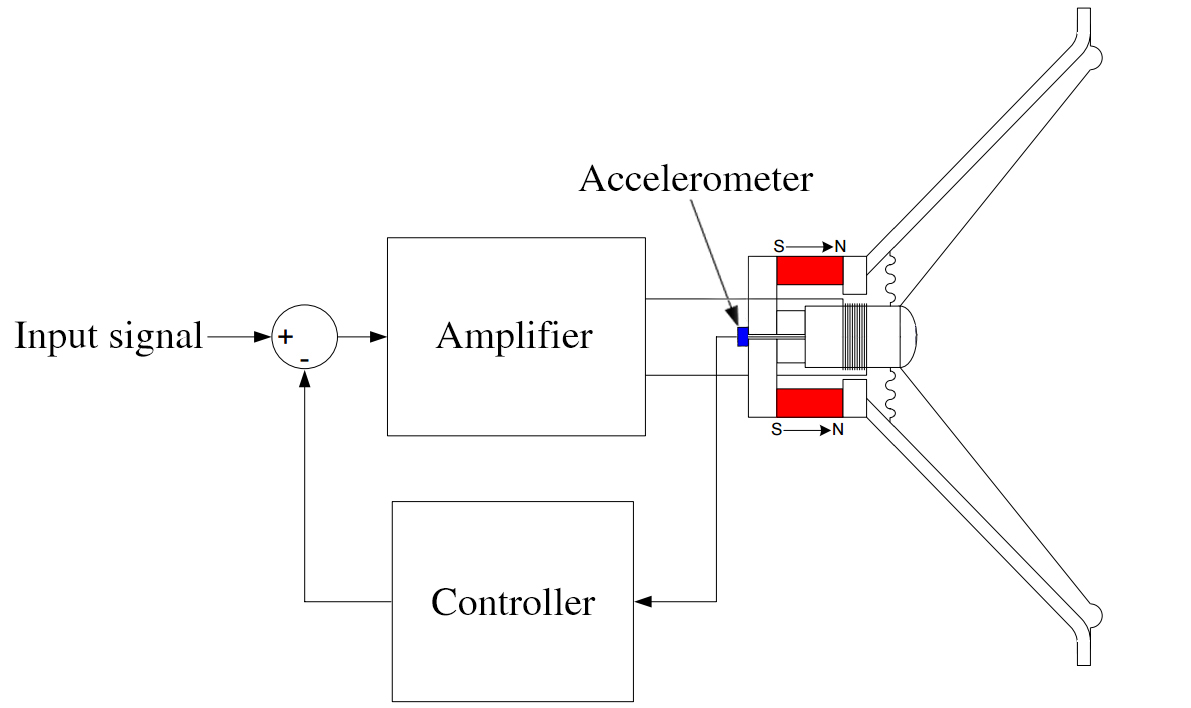
\includegraphics[width=0.75\textwidth]{Feedback_Acc2}
\caption{How a possible feedback system should be implemented in the speaker}
\label{fig:feedbacksystem}
\end{figure}


%\subsection{Distortion from vibration and impulses}\label{subsec:impulses}
%
%A common problem when designing loudspeakers are the vibrations from the enclosure. If the vibrations are strong, they will become audible and distort the overall sound. The sound radiation from the enclosure will become greater when the \gls{SPL} from the speaker increase. This problem is solved with different techniques but yield more or less the same outcome, which is stiffening of the enclosure. Some of the techniques for removing vibrations from the enclosure could be:
%\begin{itemize}
%\item Mechanical decoupling of the drivers from the enclosure.
%\item Denser or heavier construction material with a high natural frequency, making it harder for the enclosure to start vibrating.
%\item Dampening material or complex structural design inside the cabinet to disperse the sound.
%\end{itemize}
%\todo[inline]{Skal nok lige skaffe nogle kilder på de udtagelser}
%
%Another possibility is to use the vibration measurement as an indicator to tell the current performance of the loudspeaker. Since the loudspeaker will vibrate more at higher volumes. 
%
%
%Looking further into the woofer itself, it shows in \autoref{fig:SpeakerModelStress} that parts in the woofer also creates unwanted vibrations. The purpose of the woofer is to reproduce the electrical signal as an acoustical signal. This is done by using a diaphragm which is suspended in a very light and easy to move material. An Induction in the coil is created in a permanent magnet creating a a electro magnetic force resulting in the diaphragm moving. The goal will always be to loose as little as possible energy, giving the most perfect output. The woofer simply needs to be as powerful, light, stiff and efficient as possible.
%
%\begin{figure}[H]
%\centering
%\begin{subfigure}[t]{0.47\textwidth}
%\includegraphics[width=\linewidth]{SpeakerGOOD}
%	\caption{Regular speaker driver showing surround, diaphragm and the magnet.}
%	\label{fig:regularspeaker}
%\end{subfigure}
%\hspace{6mm} 
%\begin{subfigure}[t]{0.47\textwidth}
%\includegraphics[width=\linewidth]{SpeakerBAD}
%	\caption{Regular speaker driver with red markings showing stress areas}
%	\label{fig:badspeaker}
%\end{subfigure}
%\caption{A Speaker driver, where \ref{fig:badspeaker} shows the stress points outlined with red.}
%\label{fig:SpeakerModelStress}
%\end{figure}
%%When this signal has a large amplitude, read overload, the diaphragm reaches physical capacity. 
%In \autoref{fig:badspeaker} it shows that when a diaphragm is pushed to its maximum capacity the surround will affect the diaphragm causing unwanted distortion. This will be one of the major problems if the diaphragm is not sufficiently stiff to withstand the high \gls{SPL} and not twist during playback. 



%\section{Part Conclusion}
This chapter has analyzed an active speaker and its components to investigate how distortion is created throughout the active loudspeaker. The conclusion is that the following situations create distortion.
\begin{itemize}
\item Amplifier
	\begin{itemize}
	\item Clipping.
	\end{itemize}
\item Loudspeaker
	\begin{itemize}
	\item Vibrations from enclosure.
	\item Overexcursion.
	\item Membrane hitting the coil.
	\end{itemize}
\end{itemize}
Of these situations the focus moving forward will only be concerning the distortion situation from the loudspeaker because clipping in the amplifier is easy to solve, because the parameters in the amplifier is constant and the signal is easily limited to create less distortion then by hard clipping. The next chapter will therefore explain and analyze performance tests of a loudspeaker to see if any of the above loudspeaker situations can be detected. 

\subsection*{Test of DALI Zensor 5}
In order to determine whether or not it is possible to use sensory equipment to measure any vibration from the loudspeaker. It is desirable to investigate if the output of the sensors can be analyzed. The loudspeaker which will be the basis for the test is the DALI Zensor 5, shown on \autoref{fig:dali_zensor5}. A passive loudspeaker has been choosen for the test because the amplifier in DALI's active loudspeakers are designed not to push the loudspeaker to its limits and beyond. %and to be able to test how the vibrations affect distortion, the loudspeaker must be tested to above its limits.

\begin{figure}[H]
\centering
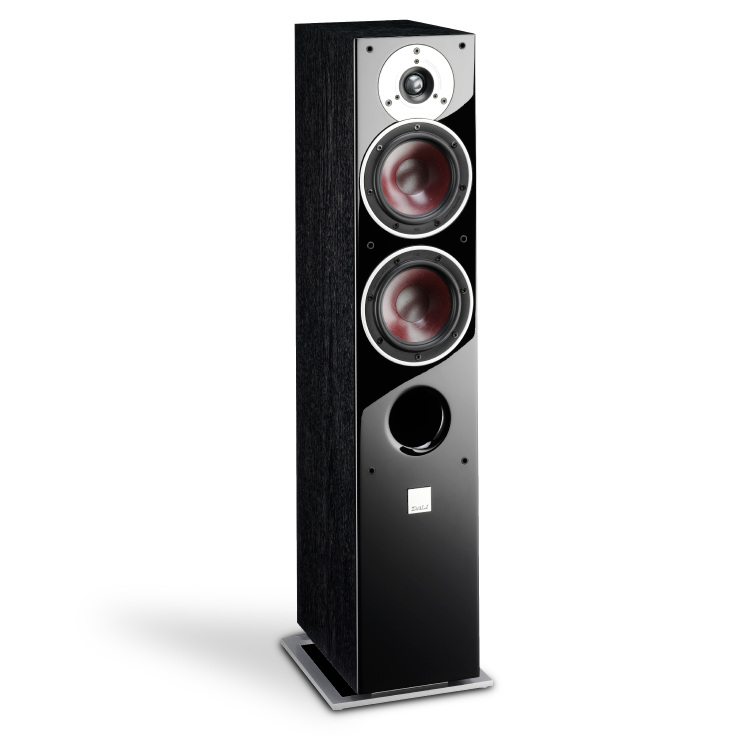
\includegraphics[width=0.5\textwidth]{figures/zensor5.png}
\caption{DALI Zensor 5 \citep{sou:daliZensor5}.}
\label{fig:dali_zensor5}
\end{figure}

%\todo[inline]{Reference http://www.dali-speakers.com/loudspeakers/zensor/zensor-5/}

For measuring the vibrations two Bruel \& Kjær (B\&K) accelerometers have been placed inside the enclosure, one on the back of the bottom driver and one on the top back of the enclosure. For measuring sound a microphone has been placed 1 m from the speaker. To limit any reflections from the room, the test is performed in a Anechoic room at \gls{AAU}, for further documentation refer to the journal in \autoref{app:journal_speaker_test}.  
%\todo[inline]{Reference (09.03.2016) http://doc.es.aau.dk/labs/acoustics/facilities/anechoic_room_large/} 



The loudspeaker is set to play a sinesweep from the crossover frequency of the loudspeaker which is 2400 Hz to 10 Hz. The sine sweep is then repeated from the lowest volume setting of a power amplifier until the loudspeaker breaks. There are in total 20 datasets each containing four measurements, namely the vibrations from the enclosure, driver, the sound pressure from the microphone and lastly a reference signal to synchronize all data. The amount of data is therefore large and only relevant datasets will be presented.  A full detailed overview of graphs is stored on the enclosed CD\footnote{\scalebox{0.7}{\path{CD://Maalinger/Maalinger030316 - Loudspeaker test/Complete Analysis.pdf}}}.



\subsubsection{Analysis of the DALI Zensor 5 measurements}

%In this section a brief review and conclusion of the analysis done in \autoref{app:journal_speaker_test} is presented. 
There are many different approaches in analysing the measured data, and the approach done in this project, will consist of analysing the frequency response of the loudspeaker vibration, harmonic distortion, and detection of the coil hitting the back plate of the driver. The structure of the following part will be showing how the speaker reacts to the different levels of amplification and to conclude if a pattern can be extracted.

%\subsection*{Experiment analysis}

%As previously stated there are in total 20 datasets each containing four measurements, namely the vibrations from the enclosure and driver, the sound pressure from the microphone, and lastly a reference signal to synchronize all data. The amount of data is therefore large and only relevant datasets will be presented. If needed, a more comprehensive approach is taken in \autoref{app:journal_speaker_test} and a full detailed overview of graphs is stored on the enclosed CD.

%\vspace{3mm}

During the first accelerometer measurements the loudspeaker acts linear with very little fluctuations. The frequency response keeps being steadily the same with an increase in amplitude which was expected. In \autoref{fig:Driver1} the first accelerometer measurement is shown, played using 5 mW at XX dB$_{\text{SPL}}$\todo{Fix dB SPL}, on the driver is seen. \autoref{fig:Enclosure1Report} shows the enclosure having a mechanical resonance frequencies at approximately 13 seconds and at 25 seconds while the driver's resonance frequency occurs at 25 seconds. An antiresonance frequency is located at 13 seconds for the accelerometers placed on the driver. The antiresonance frequency is assumed to be caused by the enclosure resonance frequency. This pattern continues for approximately 15 measurements. 

%\todo{Billede af reference tids figur og forklaring af resonans frekvens} %A tendency shows that the 3rd harmonic increases more rapidly than the 2nd harmonic, again as expected for the performance of a loudspeaker.

\begin{figure}[H]
\centering
\begin{subfigure}[t]{0.55\textwidth}
	\tikzsetnextfilename{Driver1Report}
	% This file was created by matlab2tikz.
%
%The latest updates can be retrieved from
%  http://www.mathworks.com/matlabcentral/fileexchange/22022-matlab2tikz-matlab2tikz
%where you can also make suggestions and rate matlab2tikz.
%
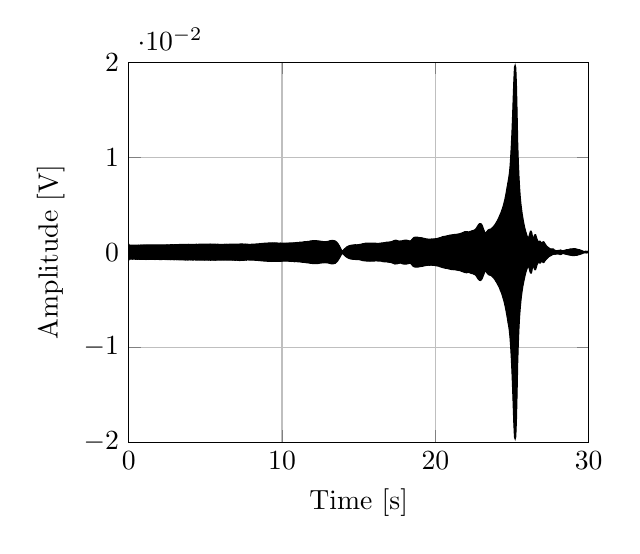
\begin{tikzpicture}

\begin{axis}[%
width=2.3in,
height=1.9in,
at={(0.758in,0.481in)},
scale only axis,
xmin=0,
xmax=30,
xmajorgrids,
ymin=-0.02,
ymax=0.02,
ymajorgrids,
xlabel={Time [s]},
ylabel={Amplitude [V]},
axis background/.style={fill=white}
]
\addplot[fill=black,draw=black,forget plot] plot table[row sep=crcr]{%
2.08333333333333e-05	0.000842452049255371\\
0.0417454218822439	0.000724315643310547\\
0.0834700104311544	0.000728130340576172\\
0.125194598980065	0.000715255737304688\\
0.166919187528975	0.000736355781555176\\
0.208643776077886	0.000741124153137207\\
0.250368364626797	0.000725150108337402\\
0.292092953175707	0.00073695182800293\\
0.333817541724618	0.000734806060791016\\
0.375542130273528	0.000743985176086426\\
0.417266718822439	0.000729680061340332\\
0.458991307371349	0.00072777271270752\\
0.50071589592026	0.000744819641113281\\
0.54244048446917	0.000737667083740234\\
0.584165073018081	0.000739336013793945\\
0.625889661566991	0.000748038291931152\\
0.667614250115902	0.000733852386474609\\
0.709338838664812	0.000737309455871582\\
0.751063427213723	0.00073850154876709\\
0.792788015762633	0.000756502151489258\\
0.834512604311544	0.000747323036193848\\
0.876237192860454	0.000743627548217773\\
0.917961781409365	0.000749349594116211\\
0.959686369958275	0.000751495361328125\\
1.00141095850719	0.000746369361877441\\
1.0431355470561	0.000753998756408691\\
1.08486013560501	0.000748515129089355\\
1.12658472415392	0.00075221061706543\\
1.16830931270283	0.000759720802307129\\
1.21003390125174	0.000748515129089355\\
1.25175848980065	0.000764369964599609\\
1.29348307834956	0.000760555267333984\\
1.33520766689847	0.000766396522521973\\
1.37693225544738	0.000762343406677246\\
1.41865684399629	0.000754714012145996\\
1.4603814325452	0.000761151313781738\\
1.50210602109411	0.000756978988647461\\
1.54383060964302	0.000756144523620605\\
1.58555519819193	0.000763535499572754\\
1.62727978674084	0.000756502151489258\\
1.66900437528975	0.000757694244384766\\
1.71072896383866	0.000751137733459473\\
1.75245355238758	0.000756502151489258\\
1.79417814093649	0.000756144523620605\\
1.8359027294854	0.000758051872253418\\
1.87762731803431	0.00075685977935791\\
1.91935190658322	0.000754356384277344\\
1.96107649513213	0.000756144523620605\\
2.00280108368104	0.000751018524169922\\
2.04452567222995	0.000769376754760742\\
2.08625026077886	0.000757336616516113\\
2.12797484932777	0.000759363174438477\\
2.16969943787668	0.000766515731811523\\
2.21142402642559	0.00075685977935791\\
2.2531486149745	0.000760316848754883\\
2.29487320352341	0.000762820243835449\\
2.33659779207232	0.000757813453674316\\
2.37832238062123	0.000756382942199707\\
2.42004696917014	0.000770211219787598\\
2.46177155771905	0.00077366828918457\\
2.50349614626796	0.000762701034545898\\
2.54522073481687	0.000776529312133789\\
2.58694532336579	0.000768661499023438\\
2.6286699119147	0.000769495964050293\\
2.67039450046361	0.000769376754760742\\
2.71211908901252	0.000779390335083008\\
2.75384367756143	0.000778675079345703\\
2.79556826611034	0.000775575637817383\\
2.83729285465925	0.0007781982421875\\
2.87901744320816	0.00077354907989502\\
2.92074203175707	0.000772714614868164\\
2.96246662030598	0.000776886940002441\\
3.00419120885489	0.000785589218139648\\
3.0459157974038	0.000795722007751465\\
3.08764038595271	0.000782370567321777\\
3.12936497450162	0.00078272819519043\\
3.17108956305053	0.000790238380432129\\
3.21281415159944	0.00079810619354248\\
3.25453874014835	0.000793933868408203\\
3.29626332869726	0.000802278518676758\\
3.33798791724618	0.000802397727966309\\
3.37971250579509	0.00080108642578125\\
3.421437094344	0.000811576843261719\\
3.46316168289291	0.000808596611022949\\
3.50488627144182	0.000804781913757324\\
3.54661085999073	0.000814437866210938\\
3.58833544853964	0.000810384750366211\\
3.63006003708855	0.000816583633422852\\
3.67178462563746	0.000807762145996094\\
3.71350921418637	0.000812888145446777\\
3.75523380273528	0.000812768936157227\\
3.79695839128419	0.000815749168395996\\
3.8386829798331	0.000813961029052734\\
3.88040756838201	0.000826478004455566\\
3.92213215693092	0.000814437866210938\\
3.96385674547983	0.000813722610473633\\
4.00558133402874	0.000811934471130371\\
4.04730592257765	0.000820755958557129\\
4.08903051112656	0.000818610191345215\\
4.13075509967547	0.000812888145446777\\
4.17247968822439	0.000814914703369141\\
4.2142042767733	0.000813126564025879\\
4.25592886532221	0.000823259353637695\\
4.29765345387112	0.000821471214294434\\
4.33937804242003	0.000811576843261719\\
4.38110263096894	0.000824570655822754\\
4.42282721951785	0.000835657119750977\\
4.46455180806676	0.000819563865661621\\
4.50627639661567	0.000821113586425781\\
4.54800098516458	0.000826597213745117\\
4.58972557371349	0.000843286514282227\\
4.6314501622624	0.00083458423614502\\
4.67317475081131	0.000841140747070313\\
4.71489933936022	0.000822782516479492\\
4.75662392790913	0.00083160400390625\\
4.79834851645804	0.000840425491333008\\
4.84007310500695	0.000842809677124023\\
4.88179769355586	0.000837802886962891\\
4.92352228210478	0.000848293304443359\\
4.96524687065368	0.000842094421386719\\
5.0069714592026	0.000839948654174805\\
5.04869604775151	0.000844120979309082\\
5.09042063630042	0.000840306282043457\\
5.13214522484933	0.000838994979858398\\
5.17386981339824	0.000844478607177734\\
5.21559440194715	0.000845789909362793\\
5.25731899049606	0.000832080841064453\\
5.29904357904497	0.000855803489685059\\
5.34076816759388	0.000848174095153809\\
5.38249275614279	0.000844120979309082\\
5.4242173446917	0.000833272933959961\\
5.46594193324061	0.000838756561279297\\
5.50766652178952	0.000839591026306152\\
5.54939111033843	0.000842094421386719\\
5.59111569888734	0.000841498374938965\\
5.63284028743625	0.000836610794067383\\
5.67456487598516	0.000829100608825684\\
5.71628946453407	0.000816583633422852\\
5.75801405308299	0.000837326049804688\\
5.7997386416319	0.000834465026855469\\
5.84146323018081	0.000824809074401855\\
5.88318781872972	0.000816226005554199\\
5.92491240727863	0.000822067260742188\\
5.96663699582754	0.000817298889160156\\
6.00836158437645	0.000820398330688477\\
6.05008617292536	0.000815391540527344\\
6.09181076147427	0.000821232795715332\\
6.13353535002318	0.000823259353637695\\
6.17525993857209	0.000811100006103516\\
6.216984527121	0.000824093818664551\\
6.25870911566991	0.00082862377166748\\
6.30043370421882	0.00082707405090332\\
6.34215829276773	0.000818133354187012\\
6.38388288131664	0.00082695484161377\\
6.42560746986555	0.000823736190795898\\
6.46733205841446	0.000827789306640625\\
6.50905664696338	0.000817418098449707\\
6.55078123551229	0.00083315372467041\\
6.5925058240612	0.00083458423614502\\
6.63423041261011	0.000834822654724121\\
6.67595500115902	0.000837922096252441\\
6.71767958970793	0.000827908515930176\\
6.75940417825684	0.00082862377166748\\
6.80112876680575	0.000835776329040527\\
6.84285335535466	0.000834941864013672\\
6.88457794390357	0.000837326049804688\\
6.92630253245248	0.000839829444885254\\
6.96802712100139	0.000847339630126953\\
7.0097517095503	0.00084376335144043\\
7.05147629809921	0.000843644142150879\\
7.09320088664812	0.000847101211547852\\
7.13492547519703	0.000847339630126953\\
7.17665006374594	0.000843644142150879\\
7.21837465229485	0.000848174095153809\\
7.26009924084376	0.000854969024658203\\
7.30182382939268	0.000855684280395508\\
7.34354841794159	0.000865817070007324\\
7.3852730064905	0.000864505767822266\\
7.42699759503941	0.000867962837219238\\
7.46872218358832	0.000847101211547852\\
7.51044677213723	0.000849604606628418\\
7.55217136068614	0.000842928886413574\\
7.59389594923505	0.000854134559631348\\
7.63562053778396	0.000830292701721191\\
7.67734512633287	0.000824570655822754\\
7.71906971488178	0.000828742980957031\\
7.76079430343069	0.000830650329589844\\
7.8025188919796	0.000817418098449707\\
7.84424348052851	0.00081479549407959\\
7.88596806907742	0.000807404518127441\\
7.92769265762633	0.000814914703369141\\
7.96941724617524	0.000820755958557129\\
8.01114183472416	0.000833749771118164\\
8.05286642327307	0.000829458236694336\\
8.09459101182198	0.000839948654174805\\
8.13631560037089	0.00084376335144043\\
8.1780401889198	0.000843167304992676\\
8.21976477746871	0.000849008560180664\\
8.26148936601762	0.000846505165100098\\
8.30321395456653	0.000858187675476074\\
8.34493854311544	0.000867486000061035\\
8.38666313166435	0.000872135162353516\\
8.42838772021326	0.000874876976013184\\
8.47011230876217	0.000872969627380371\\
8.51183689731108	0.000886321067810059\\
8.55356148585999	0.00090634822845459\\
8.5952860744089	0.000900864601135254\\
8.63701066295781	0.000904202461242676\\
8.67873525150672	0.000906229019165039\\
8.72045984005563	0.000902056694030762\\
8.76218442860454	0.000916242599487305\\
8.80390901715345	0.000928282737731934\\
8.84563360570237	0.000935554504394531\\
8.88735819425128	0.000940561294555664\\
8.92908278280018	0.000948786735534668\\
8.9708073713491	0.000948309898376465\\
9.01253195989801	0.000955462455749512\\
9.05425654844692	0.000948071479797363\\
9.09598113699583	0.0009613037109375\\
9.13770572554474	0.000966429710388184\\
9.17943031409365	0.000962972640991211\\
9.22115490264256	0.000972151756286621\\
9.26287949119147	0.000980615615844727\\
9.30460407974038	0.000973939895629883\\
9.34632866828929	0.000976324081420898\\
9.3880532568382	0.000983357429504395\\
9.42977784538711	0.000970959663391113\\
9.47150243393602	0.000966668128967285\\
9.51322702248493	0.000982522964477539\\
9.55495161103384	0.000957965850830078\\
9.59667619958275	0.000975489616394043\\
9.63840078813166	0.000963330268859863\\
9.68012537668058	0.000963330268859863\\
9.72184996522949	0.000955104827880859\\
9.7635745537784	0.000950098037719727\\
9.80529914232731	0.000947952270507813\\
9.84702373087622	0.000951766967773438\\
9.88874831942513	0.000958442687988281\\
9.93047290797404	0.000956416130065918\\
9.97219749652295	0.000945448875427246\\
10.0139220850719	0.000948071479797363\\
10.0556466736208	0.000946640968322754\\
10.0973712621697	0.00095057487487793\\
10.1390958507186	0.000947475433349609\\
10.1808204392675	0.000943899154663086\\
10.2225450278164	0.000938296318054199\\
10.2642696163653	0.000931262969970703\\
10.3059942049142	0.00095665454864502\\
10.3477187934631	0.000945925712585449\\
10.3894433820121	0.000958085060119629\\
10.431167970561	0.000952601432800293\\
10.4728925591099	0.000962257385253906\\
10.5146171476588	0.00095665454864502\\
10.5563417362077	0.000961661338806152\\
10.5980663247566	0.000960826873779297\\
10.6397909133055	0.000966787338256836\\
10.6815155018544	0.000980615615844727\\
10.7232400904033	0.00097501277923584\\
10.7649646789523	0.000985860824584961\\
10.8066892675012	0.000976681709289551\\
10.8484138560501	0.000992298126220703\\
10.890138444599	0.00099635124206543\\
10.9318630331479	0.000995159149169922\\
10.9735876216968	0.00101470947265625\\
11.0153122102457	0.00101017951965332\\
11.0570367987946	0.000998139381408691\\
11.0987613873435	0.00101804733276367\\
11.1404859758924	0.0010455846786499\\
11.1822105644414	0.00105226039886475\\
11.2239351529903	0.00104320049285889\\
11.2656597415392	0.0010448694229126\\
11.3073843300881	0.00104343891143799\\
11.349108918637	0.00106239318847656\\
11.3908335071859	0.00107407569885254\\
11.4325580957348	0.00108933448791504\\
11.4742826842837	0.00108993053436279\\
11.5160072728326	0.00110101699829102\\
11.5577318613816	0.00110852718353271\\
11.5994564499305	0.0011056661605835\\
11.6411810384794	0.00111484527587891\\
11.6829056270283	0.00112783908843994\\
11.7246302155772	0.00113523006439209\\
11.7663548041261	0.00114238262176514\\
11.808079392675	0.00115120410919189\\
11.8498039812239	0.00117611885070801\\
11.8915285697728	0.00117993354797363\\
11.9332531583217	0.0011899471282959\\
11.9749777468707	0.00120007991790771\\
12.0167023354196	0.00119864940643311\\
12.0584269239685	0.0011974573135376\\
12.1001515125174	0.00120961666107178\\
12.1418761010663	0.00121510028839111\\
12.1836006896152	0.00121378898620605\\
12.2253252781641	0.00121426582336426\\
12.267049866713	0.00120794773101807\\
12.3087744552619	0.00118112564086914\\
12.3504990438108	0.0011749267578125\\
12.3922236323598	0.00118374824523926\\
12.4339482209087	0.00116109848022461\\
12.4756728094576	0.00115525722503662\\
12.5173973980065	0.00115251541137695\\
12.5591219865554	0.00112485885620117\\
12.6008465751043	0.00112450122833252\\
12.6425711636532	0.00111746788024902\\
12.6842957522021	0.00111103057861328\\
12.726020340751	0.00111186504364014\\
12.7677449293	0.00110268592834473\\
12.8094695178489	0.00109696388244629\\
12.8511941063978	0.00110363960266113\\
12.8929186949467	0.00111150741577148\\
12.9346432834956	0.00111949443817139\\
12.9763678720445	0.001137375831604\\
13.0180924605934	0.00114357471466064\\
13.0598170491423	0.0011603832244873\\
13.1015416376912	0.00118207931518555\\
13.1432662262401	0.00121927261352539\\
13.1849908147891	0.00120532512664795\\
13.226715403338	0.00122213363647461\\
13.2684399918869	0.00122547149658203\\
13.3101645804358	0.00123798847198486\\
13.3518891689847	0.00121581554412842\\
13.3936137575336	0.0012049674987793\\
13.4353383460825	0.00118744373321533\\
13.4770629346314	0.00116372108459473\\
13.5187875231803	0.00110864639282227\\
13.5605121117293	0.00106608867645264\\
13.6022367002782	0.000977635383605957\\
13.6439612888271	0.000897884368896484\\
13.685685877376	0.000793695449829102\\
13.7274104659249	0.000687122344970703\\
13.7691350544738	0.000558257102966309\\
13.8108596430227	0.000436067581176758\\
13.8525842315716	0.000294923782348633\\
13.8943088201205	0.00018310546875\\
13.9360334086694	0.000113487243652344\\
13.9777579972184	0.000168681144714355\\
14.0194825857673	0.000242471694946289\\
14.0612071743162	0.000313043594360352\\
14.1029317628651	0.000383496284484863\\
14.144656351414	0.000434041023254395\\
14.1863809399629	0.00050199031829834\\
14.2281055285118	0.000554561614990234\\
14.2698301170607	0.000588655471801758\\
14.3115547056096	0.000618696212768555\\
14.3532792941586	0.000660181045532227\\
14.3950038827075	0.000678420066833496\\
14.4367284712564	0.00069725513458252\\
14.4784530598053	0.000716447830200195\\
14.5201776483542	0.000728964805603027\\
14.5619022369031	0.000737190246582031\\
14.603626825452	0.000746846199035645\\
14.6453514140009	0.00075066089630127\\
14.6870760025498	0.000756025314331055\\
14.7288005910988	0.000767707824707031\\
14.7705251796477	0.00078284740447998\\
14.8122497681966	0.000776410102844238\\
14.8539743567455	0.000770330429077148\\
14.8956989452944	0.00076603889465332\\
14.9374235338433	0.000783920288085938\\
14.9791481223922	0.000787258148193359\\
15.0208727109411	0.000798940658569336\\
15.06259729949	0.00080108642578125\\
15.1043218880389	0.000807285308837891\\
15.1460464765879	0.00083625316619873\\
15.1877710651368	0.00084996223449707\\
15.2294956536857	0.000864148139953613\\
15.2712202422346	0.000891566276550293\\
15.3129448307835	0.000901222229003906\\
15.3546694193324	0.000907182693481445\\
15.3963940078813	0.00091242790222168\\
15.4381185964302	0.000938892364501953\\
15.4798431849791	0.000932097434997559\\
15.521567773528	0.000941276550292969\\
15.563292362077	0.000940442085266113\\
15.6050169506259	0.000934958457946777\\
15.6467415391748	0.000942468643188477\\
15.6884661277237	0.000942111015319824\\
15.7301907162726	0.000946402549743652\\
15.7719153048215	0.000940442085266113\\
15.8136398933704	0.000940442085266113\\
15.8553644819193	0.000932574272155762\\
15.8970890704682	0.00094294548034668\\
15.9388136590172	0.000941276550292969\\
15.9805382475661	0.000934720039367676\\
16.022262836115	0.000936269760131836\\
16.0639874246639	0.000932216644287109\\
16.1057120132128	0.000941753387451172\\
16.1474366017617	0.000922083854675293\\
16.1891611903106	0.000919580459594727\\
16.2308857788595	0.000926733016967773\\
16.2726103674084	0.000928401947021484\\
16.3143349559573	0.000926613807678223\\
16.3560595445063	0.000929117202758789\\
16.3977841330552	0.000951766967773438\\
16.4395087216041	0.000945568084716797\\
16.481233310153	0.000967264175415039\\
16.5229578987019	0.000959634780883789\\
16.5646824872508	0.000981688499450684\\
16.6064070757997	0.000978827476501465\\
16.6481316643486	0.00100505352020264\\
16.6898562528975	0.000998139381408691\\
16.7315808414465	0.00101649761199951\\
16.7733054299954	0.00102102756500244\\
16.8150300185443	0.0010451078414917\\
16.8567546070932	0.00104188919067383\\
16.8984791956421	0.00102841854095459\\
16.940203784191	0.00104808807373047\\
16.9819283727399	0.00106561183929443\\
17.0236529612888	0.00106358528137207\\
17.0653775498377	0.00106775760650635\\
17.1071021383867	0.00110936164855957\\
17.1488267269356	0.00111019611358643\\
17.1905513154845	0.0011366605758667\\
17.2322759040334	0.00117075443267822\\
17.2740004925823	0.00120162963867188\\
17.3157250811312	0.00121581554412842\\
17.3574496696801	0.00124251842498779\\
17.399174258229	0.00124752521514893\\
17.4408988467779	0.00124835968017578\\
17.4826234353268	0.00122547149658203\\
17.5243480238758	0.00121092796325684\\
17.5660726124247	0.00118362903594971\\
17.6077972009736	0.00117075443267822\\
17.6495217895225	0.00116026401519775\\
17.6912463780714	0.00117111206054688\\
17.7329709666203	0.00116336345672607\\
17.7746955551692	0.00118422508239746\\
17.8164201437181	0.00119113922119141\\
17.858144732267	0.00120329856872559\\
17.8998693208159	0.00122535228729248\\
17.9415939093649	0.00124597549438477\\
17.9833184979138	0.00124430656433105\\
18.0250430864627	0.00126302242279053\\
18.0667676750116	0.00126171112060547\\
18.1084922635605	0.00125372409820557\\
18.1502168521094	0.00124704837799072\\
18.1919414406583	0.00123119354248047\\
18.2336660292072	0.00121426582336426\\
18.2753906177561	0.00119447708129883\\
18.3171152063051	0.00117504596710205\\
18.358839794854	0.00118374824523926\\
18.4005643834029	0.00120377540588379\\
18.4422889719518	0.00127255916595459\\
18.4840135605007	0.00135231018066406\\
18.5257381490496	0.00141823291778564\\
18.5674627375985	0.00150668621063232\\
18.6091873261474	0.00154757499694824\\
18.6509119146963	0.0015639066696167\\
18.6926365032453	0.00156760215759277\\
18.7343610917942	0.00158751010894775\\
18.7760856803431	0.00158250331878662\\
18.817810268892	0.00157392024993896\\
18.8595348574409	0.00155794620513916\\
18.9012594459898	0.00155055522918701\\
18.9429840345387	0.00154078006744385\\
18.9847086230876	0.00152921676635742\\
19.0264332116365	0.00152289867401123\\
19.0681578001854	0.00152289867401123\\
19.1098823887344	0.00150799751281738\\
19.1516069772833	0.00149905681610107\\
19.1933315658322	0.00147044658660889\\
19.2350561543811	0.00145161151885986\\
19.27678074293	0.00144112110137939\\
19.3185053314789	0.00142991542816162\\
19.3602299200278	0.00141644477844238\\
19.4019545085767	0.0013880729675293\\
19.4436790971256	0.00139951705932617\\
19.4854036856745	0.00137901306152344\\
19.5271282742235	0.00136971473693848\\
19.5688528627724	0.00136721134185791\\
19.6105774513213	0.00136351585388184\\
19.6523020398702	0.00136446952819824\\
19.6940266284191	0.0013653039932251\\
19.735751216968	0.00137889385223389\\
19.7774758055169	0.00138390064239502\\
19.8192003940658	0.0013740062713623\\
19.8609249826147	0.00138437747955322\\
19.9026495711637	0.00140023231506348\\
19.9443741597126	0.00139617919921875\\
19.9860987482615	0.00141024589538574\\
20.0278233368104	0.00141370296478271\\
20.0695479253593	0.00140857696533203\\
20.1112725139082	0.00143897533416748\\
20.1529971024571	0.00145316123962402\\
20.194721691006	0.00147128105163574\\
20.2364462795549	0.00149738788604736\\
20.2781708681038	0.00151407718658447\\
20.3198954566528	0.00153207778930664\\
20.3616200452017	0.00156009197235107\\
20.4033446337506	0.0015721321105957\\
20.4450692222995	0.00161302089691162\\
20.4867938108484	0.00163066387176514\\
20.5285183993973	0.00164401531219482\\
20.5702429879462	0.00166523456573486\\
20.6119675764951	0.00166523456573486\\
20.653692165044	0.0016857385635376\\
20.695416753593	0.00168442726135254\\
20.7371413421419	0.00170993804931641\\
20.7788659306908	0.00172114372253418\\
20.8205905192397	0.00173604488372803\\
20.8623151077886	0.00174999237060547\\
20.9040396963375	0.00177335739135742\\
20.9457642848864	0.00178420543670654\\
20.9874888734353	0.00179541110992432\\
21.0292134619842	0.0018075704574585\\
21.0709380505331	0.00182294845581055\\
21.1126626390821	0.00182592868804932\\
21.154387227631	0.00183844566345215\\
21.1961118161799	0.00185132026672363\\
21.2378364047288	0.00185286998748779\\
21.2795609932777	0.00185167789459229\\
21.3212855818266	0.00186431407928467\\
21.3630101703755	0.0018768310546875\\
21.4047347589244	0.00187921524047852\\
21.4464593474733	0.00189435482025146\\
21.4881839360223	0.00190842151641846\\
21.5299085245712	0.00191879272460938\\
21.5716331131201	0.0019301176071167\\
21.613357701669	0.00195229053497314\\
21.6550822902179	0.00198221206665039\\
21.6968068787668	0.00199604034423828\\
21.7385314673157	0.00202810764312744\\
21.7802560558646	0.00205862522125244\\
21.8219806444135	0.00206995010375977\\
21.8637052329624	0.00211036205291748\\
21.9054298215114	0.0021432638168335\\
21.9471544100603	0.00215423107147217\\
21.9888789986092	0.00216424465179443\\
22.0306035871581	0.00215709209442139\\
22.072328175707	0.00216305255889893\\
22.1140527642559	0.00213837623596191\\
22.1557773528048	0.00213634967803955\\
22.1975019413537	0.00212752819061279\\
22.2392265299026	0.0021662712097168\\
22.2809511184516	0.00218296051025391\\
22.3226757070005	0.00220799446105957\\
22.3644002955494	0.002236008644104\\
22.4061248840983	0.00226271152496338\\
22.4478494726472	0.00227344036102295\\
22.4895740611961	0.00229513645172119\\
22.531298649745	0.00232028961181641\\
22.5730232382939	0.00235486030578613\\
22.6147478268428	0.00240409374237061\\
22.6564724153917	0.00249433517456055\\
22.6981970039407	0.00258851051330566\\
22.7399215924896	0.00270044803619385\\
22.7816461810385	0.00281000137329102\\
22.8233707695874	0.00291359424591064\\
22.8650953581363	0.00298619270324707\\
22.9068199466852	0.00299859046936035\\
22.9485445352341	0.00299358367919922\\
22.990269123783	0.00297236442565918\\
23.0319937123319	0.00287067890167236\\
23.0737183008809	0.00273036956787109\\
23.1154428894298	0.0025404691696167\\
23.1571674779787	0.00235271453857422\\
23.1988920665276	0.00218009948730469\\
23.2406166550765	0.00201857089996338\\
23.2823412436254	0.00202608108520508\\
23.3240658321743	0.00209319591522217\\
23.3657904207232	0.00218164920806885\\
23.4075150092721	0.00226426124572754\\
23.449239597821	0.00233328342437744\\
23.49096418637	0.0023798942565918\\
23.5326887749189	0.0024033784866333\\
23.5744133634678	0.00241625308990479\\
23.6161379520167	0.00243675708770752\\
23.6578625405656	0.0024871826171875\\
23.6995871291145	0.00255143642425537\\
23.7413117176634	0.00261306762695313\\
23.7830363062123	0.00269031524658203\\
23.8247608947612	0.00277090072631836\\
23.8664854833102	0.00285768508911133\\
23.9082100718591	0.00295233726501465\\
23.949934660408	0.0030667781829834\\
23.9916592489569	0.00317692756652832\\
24.0333838375058	0.00328707695007324\\
24.0751084260547	0.00342345237731934\\
24.1168330146036	0.00355243682861328\\
24.1585576031525	0.00371789932250977\\
24.2002821917014	0.00386691093444824\\
24.2420067802503	0.00402510166168213\\
24.2837313687993	0.00418233871459961\\
24.3254559573482	0.00438845157623291\\
24.3671805458971	0.00456619262695313\\
24.408905134446	0.00477814674377441\\
24.4506297229949	0.00500857830047607\\
24.4923543115438	0.00528395175933838\\
24.5340789000927	0.00555253028869629\\
24.5758034886416	0.00591349601745605\\
24.6175280771905	0.00626111030578613\\
24.6592526657395	0.00665700435638428\\
24.7009772542884	0.00705134868621826\\
24.7427018428373	0.00741517543792725\\
24.7844264313862	0.00782275199890137\\
24.8261510199351	0.00829911231994629\\
24.867875608484	0.00896334648132324\\
24.9096001970329	0.00995182991027832\\
24.9513247855818	0.011165976524353\\
24.9930493741307	0.012565016746521\\
25.0347739626796	0.0142723321914673\\
25.0764985512286	0.0162241458892822\\
25.1182231397775	0.0180796384811401\\
25.1599477283264	0.0194665193557739\\
25.2016723168753	0.0196808576583862\\
25.2433969054242	0.019420862197876\\
25.2851214939731	0.0176268815994263\\
25.326846082522	0.0148277282714844\\
25.3685706710709	0.0115214586257935\\
25.4102952596198	0.00949466228485107\\
25.4520198481687	0.00793111324310303\\
25.4937444367177	0.00675833225250244\\
25.5354690252666	0.00582170486450195\\
25.5771936138155	0.00510656833648682\\
25.6189182023644	0.00454449653625488\\
25.6606427909133	0.00404250621795654\\
25.7023673794622	0.00363194942474365\\
25.7440919680111	0.00321686267852783\\
25.78581655656	0.0028984546661377\\
25.8275411451089	0.00256967544555664\\
25.8692657336579	0.00231683254241943\\
25.9109903222068	0.00206875801086426\\
25.9527149107557	0.00185883045196533\\
25.9944394993046	0.00165820121765137\\
26.0361640878535	0.00150573253631592\\
26.0778886764024	0.00152122974395752\\
26.1196132649513	0.00173819065093994\\
26.1613378535002	0.00199723243713379\\
26.2030624420491	0.00220644474029541\\
26.2447870305981	0.00220096111297607\\
26.286511619147	0.00204658508300781\\
26.3282362076959	0.00164556503295898\\
26.3699607962448	0.00141119956970215\\
26.4116853847937	0.00154078006744385\\
26.4534099733426	0.00174570083618164\\
26.4951345618915	0.00183117389678955\\
26.5368591504404	0.00183594226837158\\
26.5785837389893	0.00163650512695313\\
26.6203083275383	0.00140058994293213\\
26.6620329160872	0.00124001502990723\\
26.7037575046361	0.00111579895019531\\
26.745482093185	0.00109744071960449\\
26.7872066817339	0.00114655494689941\\
26.8289312702828	0.00115036964416504\\
26.8706558588317	0.0010751485824585\\
26.9123804473806	0.000989675521850586\\
26.9541050359295	0.000946640968322754\\
26.9958296244784	0.0010601282119751\\
27.0375542130274	0.00109231472015381\\
27.0792788015763	0.00107848644256592\\
27.1210033901252	0.000966310501098633\\
27.1627279786741	0.000848174095153809\\
27.204452567223	0.000764727592468262\\
27.2461771557719	0.000650525093078613\\
27.2879017443208	0.000586748123168945\\
27.3296263328697	0.00053858757019043\\
27.3713509214186	0.000492334365844727\\
27.4130755099675	0.000432610511779785\\
27.4548000985165	0.000382304191589355\\
27.4965246870654	0.000351667404174805\\
27.5382492756143	0.000335097312927246\\
27.5799738641632	0.000327467918395996\\
27.6216984527121	0.000345587730407715\\
27.663423041261	0.000339984893798828\\
27.7051476298099	0.000326752662658691\\
27.7468722183588	0.000255465507507324\\
27.7885968069077	0.000196218490600586\\
27.8303213954567	0.000179886817932129\\
27.8720459840056	0.000151991844177246\\
27.9137705725545	0.000140666961669922\\
27.9554951611034	0.000151515007019043\\
27.9972197496523	0.00017392635345459\\
28.0389443382012	0.000173568725585938\\
28.0806689267501	0.000182271003723145\\
28.122393515299	0.000199556350708008\\
28.1641181038479	0.000229477882385254\\
28.2058426923968	0.000199556350708008\\
28.2475672809458	0.00016319751739502\\
28.2892918694947	0.000146865844726563\\
28.3310164580436	0.000162005424499512\\
28.3727410465925	0.00016939640045166\\
28.4144656351414	0.000180602073669434\\
28.4561902236903	0.000207781791687012\\
28.4979148122392	0.000230312347412109\\
28.5396394007881	0.00024878978729248\\
28.581363989337	0.00026702880859375\\
28.623088577886	0.00024712085723877\\
28.6648131664349	0.000267505645751953\\
28.7065377549838	0.000287413597106934\\
28.7482623435327	0.000310063362121582\\
28.7899869320816	0.000333070755004883\\
28.8317115206305	0.000332236289978027\\
28.8734361091794	0.000330567359924316\\
28.9151606977283	0.000338912010192871\\
28.9568852862772	0.0003509521484375\\
28.9986098748261	0.000365018844604492\\
29.0403344633751	0.000368833541870117\\
29.082059051924	0.000351786613464355\\
29.1237836404729	0.000357151031494141\\
29.1655082290218	0.00033724308013916\\
29.2072328175707	0.000323772430419922\\
29.2489574061196	0.000299692153930664\\
29.2906819946685	0.000292539596557617\\
29.3324065832174	0.000269055366516113\\
29.3741311717663	0.000259637832641602\\
29.4158557603153	0.000249624252319336\\
29.4575803488642	0.000213623046875\\
29.4993049374131	0.000187873840332031\\
29.541029525962	0.000171542167663574\\
29.5827541145109	0.000138521194458008\\
29.6244787030598	0.000112175941467285\\
29.6662032916087	8.85725021362305e-05\\
29.7079278801576	7.25984573364258e-05\\
29.7496524687065	6.3776969909668e-05\\
29.7913770572554	0.000100255012512207\\
29.8331016458044	8.69035720825195e-05\\
29.8748262343533	8.80956649780273e-05\\
29.9165508229022	9.09566879272461e-05\\
29.9582754114511	7.89165496826172e-05\\
30	6.34193420410156e-05\\
}
\closedcycle;
\addplot[fill=black,draw=black,forget plot] plot table[row sep=crcr]{%
2.08333333333333e-05	-0.000848650932312012\\
0.0417454218822439	-0.000736355781555176\\
0.0834700104311544	-0.000727176666259766\\
0.125194598980065	-0.000741720199584961\\
0.166919187528975	-0.000732183456420898\\
0.208643776077886	-0.000723361968994141\\
0.250368364626797	-0.0007476806640625\\
0.292092953175707	-0.000734686851501465\\
0.333817541724618	-0.000736474990844727\\
0.375542130273528	-0.00073397159576416\\
0.417266718822439	-0.000738024711608887\\
0.458991307371349	-0.000752568244934082\\
0.50071589592026	-0.000742197036743164\\
0.54244048446917	-0.000741481781005859\\
0.584165073018081	-0.000744819641113281\\
0.625889661566991	-0.000743985176086426\\
0.667614250115902	-0.000739812850952148\\
0.709338838664812	-0.000747323036193848\\
0.751063427213723	-0.000758171081542969\\
0.792788015762633	-0.000746011734008789\\
0.834512604311544	-0.000747203826904297\\
0.876237192860454	-0.000759005546569824\\
0.917961781409365	-0.000752568244934082\\
0.959686369958275	-0.000758051872253418\\
1.00141095850719	-0.000755906105041504\\
1.0431355470561	-0.000764250755310059\\
1.08486013560501	-0.000764250755310059\\
1.12658472415392	-0.000774264335632324\\
1.16830931270283	-0.000757694244384766\\
1.21003390125174	-0.000753998756408691\\
1.25175848980065	-0.000754237174987793\\
1.29348307834956	-0.000767707824707031\\
1.33520766689847	-0.000755071640014648\\
1.37693225544738	-0.000764369964599609\\
1.41865684399629	-0.000763893127441406\\
1.4603814325452	-0.000762701034545898\\
1.50210602109411	-0.000756382942199707\\
1.54383060964302	-0.000757575035095215\\
1.58555519819193	-0.000766873359680176\\
1.62727978674084	-0.000766873359680176\\
1.66900437528975	-0.000758886337280273\\
1.71072896383866	-0.00077521800994873\\
1.75245355238758	-0.000761866569519043\\
1.79417814093649	-0.000762224197387695\\
1.8359027294854	-0.000767707824707031\\
1.87762731803431	-0.000755667686462402\\
1.91935190658322	-0.000763416290283203\\
1.96107649513213	-0.000767350196838379\\
2.00280108368104	-0.000774025917053223\\
2.04452567222995	-0.000765085220336914\\
2.08625026077886	-0.000775694847106934\\
2.12797484932777	-0.000765681266784668\\
2.16969943787668	-0.000776410102844238\\
2.21142402642559	-0.000763058662414551\\
2.2531486149745	-0.000763058662414551\\
2.29487320352341	-0.000760912895202637\\
2.33659779207232	-0.000757694244384766\\
2.37832238062123	-0.000784873962402344\\
2.42004696917014	-0.000759243965148926\\
2.46177155771905	-0.000768899917602539\\
2.50349614626796	-0.000772595405578613\\
2.54522073481687	-0.000766873359680176\\
2.58694532336579	-0.000774860382080078\\
2.6286699119147	-0.000769853591918945\\
2.67039450046361	-0.000781416893005371\\
2.71211908901252	-0.000794768333435059\\
2.75384367756143	-0.000785231590270996\\
2.79556826611034	-0.000778436660766602\\
2.83729285465925	-0.000780582427978516\\
2.87901744320816	-0.000785112380981445\\
2.92074203175707	-0.000790715217590332\\
2.96246662030598	-0.00080108642578125\\
3.00419120885489	-0.000789880752563477\\
3.0459157974038	-0.0007781982421875\\
3.08764038595271	-0.000789880752563477\\
3.12936497450162	-0.000799417495727539\\
3.17108956305053	-0.000792384147644043\\
3.21281415159944	-0.000795245170593262\\
3.25453874014835	-0.00079345703125\\
3.29626332869726	-0.000799894332885742\\
3.33798791724618	-0.000810623168945313\\
3.37971250579509	-0.000804901123046875\\
3.421437094344	-0.000817656517028809\\
3.46316168289291	-0.000798583030700684\\
3.50488627144182	-0.000811100006103516\\
3.54661085999073	-0.00082099437713623\\
3.58833544853964	-0.000811100006103516\\
3.63006003708855	-0.000810146331787109\\
3.67178462563746	-0.00082850456237793\\
3.71350921418637	-0.00082850456237793\\
3.75523380273528	-0.000806570053100586\\
3.79695839128419	-0.00083160400390625\\
3.8386829798331	-0.000824809074401855\\
3.88040756838201	-0.000826597213745117\\
3.92213215693092	-0.000815629959106445\\
3.96385674547983	-0.00081026554107666\\
4.00558133402874	-0.000826120376586914\\
4.04730592257765	-0.00081944465637207\\
4.08903051112656	-0.000818610191345215\\
4.13075509967547	-0.000826478004455566\\
4.17247968822439	-0.000844836235046387\\
4.2142042767733	-0.000839471817016602\\
4.25592886532221	-0.000809073448181152\\
4.29765345387112	-0.000808238983154297\\
4.33937804242003	-0.000825762748718262\\
4.38110263096894	-0.000840663909912109\\
4.42282721951785	-0.000823259353637695\\
4.46455180806676	-0.000833272933959961\\
4.50627639661567	-0.000827670097351074\\
4.54800098516458	-0.000819921493530273\\
4.58972557371349	-0.00082862377166748\\
4.6314501622624	-0.000837802886962891\\
4.67317475081131	-0.000841140747070313\\
4.71489933936022	-0.000836014747619629\\
4.75662392790913	-0.00083613395690918\\
4.79834851645804	-0.000834107398986816\\
4.84007310500695	-0.000843286514282227\\
4.88179769355586	-0.000843286514282227\\
4.92352228210478	-0.000844001770019531\\
4.96524687065368	-0.000848531723022461\\
5.0069714592026	-0.000839948654174805\\
5.04869604775151	-0.000840306282043457\\
5.09042063630042	-0.000840306282043457\\
5.13214522484933	-0.000833630561828613\\
5.17386981339824	-0.000844120979309082\\
5.21559440194715	-0.000847816467285156\\
5.25731899049606	-0.00084233283996582\\
5.29904357904497	-0.000841498374938965\\
5.34076816759388	-0.000856161117553711\\
5.38249275614279	-0.000845193862915039\\
5.4242173446917	-0.000843524932861328\\
5.46594193324061	-0.000838160514831543\\
5.50766652178952	-0.000849485397338867\\
5.54939111033843	-0.00084078311920166\\
5.59111569888734	-0.000829935073852539\\
5.63284028743625	-0.000863313674926758\\
5.67456487598516	-0.000837326049804688\\
5.71628946453407	-0.000847339630126953\\
5.75801405308299	-0.000831007957458496\\
5.7997386416319	-0.000832438468933105\\
5.84146323018081	-0.00081932544708252\\
5.88318781872972	-0.000827789306640625\\
5.92491240727863	-0.000827431678771973\\
5.96663699582754	-0.000844955444335938\\
6.00836158437645	-0.000824451446533203\\
6.05008617292536	-0.000841498374938965\\
6.09181076147427	-0.000824332237243652\\
6.13353535002318	-0.000823974609375\\
6.17525993857209	-0.000834822654724121\\
6.216984527121	-0.00083315372467041\\
6.25870911566991	-0.000827312469482422\\
6.30043370421882	-0.000815987586975098\\
6.34215829276773	-0.000829935073852539\\
6.38388288131664	-0.000832796096801758\\
6.42560746986555	-0.000832676887512207\\
6.46733205841446	-0.000835657119750977\\
6.50905664696338	-0.000832319259643555\\
6.55078123551229	-0.00084078311920166\\
6.5925058240612	-0.000838994979858398\\
6.63423041261011	-0.000837802886962891\\
6.67595500115902	-0.000836610794067383\\
6.71767958970793	-0.000833511352539063\\
6.75940417825684	-0.000843524932861328\\
6.80112876680575	-0.000849485397338867\\
6.84285335535466	-0.00084233283996582\\
6.88457794390357	-0.000846624374389648\\
6.92630253245248	-0.000850319862365723\\
6.96802712100139	-0.00084686279296875\\
7.0097517095503	-0.000850796699523926\\
7.05147629809921	-0.000838279724121094\\
7.09320088664812	-0.000857353210449219\\
7.13492547519703	-0.000848531723022461\\
7.17665006374594	-0.000858306884765625\\
7.21837465229485	-0.000882744789123535\\
7.26009924084376	-0.000882506370544434\\
7.30182382939268	-0.000867009162902832\\
7.34354841794159	-0.000865817070007324\\
7.3852730064905	-0.000858306884765625\\
7.42699759503941	-0.000864386558532715\\
7.46872218358832	-0.000867724418640137\\
7.51044677213723	-0.000861525535583496\\
7.55217136068614	-0.000847697257995605\\
7.59389594923505	-0.000844359397888184\\
7.63562053778396	-0.000846147537231445\\
7.67734512633287	-0.000851035118103027\\
7.71906971488178	-0.000816822052001953\\
7.76079430343069	-0.000815153121948242\\
7.8025188919796	-0.000821113586425781\\
7.84424348052851	-0.000821113586425781\\
7.88596806907742	-0.000821590423583984\\
7.92769265762633	-0.000823974609375\\
7.96941724617524	-0.000836968421936035\\
8.01114183472416	-0.00081944465637207\\
8.05286642327307	-0.000829815864562988\\
8.09459101182198	-0.000835776329040527\\
8.13631560037089	-0.00083613395690918\\
8.1780401889198	-0.00084531307220459\\
8.21976477746871	-0.000847339630126953\\
8.26148936601762	-0.000851154327392578\\
8.30321395456653	-0.00084996223449707\\
8.34493854311544	-0.000859498977661133\\
8.38666313166435	-0.000870347023010254\\
8.42838772021326	-0.000869512557983398\\
8.47011230876217	-0.000878691673278809\\
8.51183689731108	-0.000882506370544434\\
8.55356148585999	-0.000886082649230957\\
8.5952860744089	-0.000893235206604004\\
8.63701066295781	-0.000912904739379883\\
8.67873525150672	-0.000919580459594727\\
8.72045984005563	-0.000918745994567871\\
8.76218442860454	-0.000920295715332031\\
8.80390901715345	-0.000934243202209473\\
8.84563360570237	-0.000929474830627441\\
8.88735819425128	-0.000936985015869141\\
8.92908278280018	-0.000938773155212402\\
8.9708073713491	-0.00094449520111084\\
9.01253195989801	-0.000952005386352539\\
9.05425654844692	-0.000960111618041992\\
9.09598113699583	-0.000960946083068848\\
9.13770572554474	-0.000954508781433105\\
9.17943031409365	-0.000959515571594238\\
9.22115490264256	-0.000964164733886719\\
9.26287949119147	-0.000971794128417969\\
9.30460407974038	-0.00097966194152832\\
9.34632866828929	-0.00097048282623291\\
9.3880532568382	-0.000972151756286621\\
9.42977784538711	-0.000975370407104492\\
9.47150243393602	-0.000976324081420898\\
9.51322702248493	-0.000971674919128418\\
9.55495161103384	-0.000966787338256836\\
9.59667619958275	-0.000972509384155273\\
9.63840078813166	-0.000962018966674805\\
9.68012537668058	-0.00096595287322998\\
9.72184996522949	-0.00096285343170166\\
9.7635745537784	-0.000970005989074707\\
9.80529914232731	-0.000964999198913574\\
9.84702373087622	-0.000945925712585449\\
9.88874831942513	-0.00096428394317627\\
9.93047290797404	-0.000971317291259766\\
9.97219749652295	-0.000945091247558594\\
10.0139220850719	-0.000952482223510742\\
10.0556466736208	-0.000939607620239258\\
10.0973712621697	-0.000944614410400391\\
10.1390958507186	-0.000936150550842285\\
10.1808204392675	-0.000943660736083984\\
10.2225450278164	-0.000951170921325684\\
10.2642696163653	-0.000944614410400391\\
10.3059942049142	-0.000943422317504883\\
10.3477187934631	-0.000941634178161621\\
10.3894433820121	-0.000942587852478027\\
10.431167970561	-0.000953435897827148\\
10.4728925591099	-0.000962138175964355\\
10.5146171476588	-0.000963330268859863\\
10.5563417362077	-0.000968694686889648\\
10.5980663247566	-0.000970840454101563\\
10.6397909133055	-0.000980138778686523\\
10.6815155018544	-0.000971317291259766\\
10.7232400904033	-0.000975847244262695\\
10.7649646789523	-0.000984311103820801\\
10.8066892675012	-0.00100791454315186\\
10.8484138560501	-0.000988364219665527\\
10.890138444599	-0.000985860824584961\\
10.9318630331479	-0.000999689102172852\\
10.9735876216968	-0.000994205474853516\\
11.0153122102457	-0.00100958347320557\\
11.0570367987946	-0.00100922584533691\\
11.0987613873435	-0.00102090835571289\\
11.1404859758924	-0.00102758407592773\\
11.1822105644414	-0.0010221004486084\\
11.2239351529903	-0.00104045867919922\\
11.2656597415392	-0.00105273723602295\\
11.3073843300881	-0.00106215476989746\\
11.349108918637	-0.00106596946716309\\
11.3908335071859	-0.00107014179229736\\
11.4325580957348	-0.00107312202453613\\
11.4742826842837	-0.00108301639556885\\
11.5160072728326	-0.0010911226272583\\
11.5577318613816	-0.00110316276550293\\
11.5994564499305	-0.00111198425292969\\
11.6411810384794	-0.00113534927368164\\
11.6829056270283	-0.00112700462341309\\
11.7246302155772	-0.00113224983215332\\
11.7663548041261	-0.00114190578460693\\
11.808079392675	-0.00116229057312012\\
11.8498039812239	-0.001167893409729\\
11.8915285697728	-0.00116455554962158\\
11.9332531583217	-0.00118577480316162\\
11.9749777468707	-0.00119209289550781\\
12.0167023354196	-0.00119900703430176\\
12.0584269239685	-0.001212477684021\\
12.1001515125174	-0.0012129545211792\\
12.1418761010663	-0.00120663642883301\\
12.1836006896152	-0.00120294094085693\\
12.2253252781641	-0.001212477684021\\
12.267049866713	-0.00120329856872559\\
12.3087744552619	-0.00120460987091064\\
12.3504990438108	-0.0011974573135376\\
12.3922236323598	-0.00117373466491699\\
12.4339482209087	-0.00116944313049316\\
12.4756728094576	-0.00114285945892334\\
12.5173973980065	-0.00113606452941895\\
12.5591219865554	-0.00113809108734131\\
12.6008465751043	-0.00113391876220703\\
12.6425711636532	-0.00111567974090576\\
12.6842957522021	-0.00110936164855957\\
12.726020340751	-0.00112056732177734\\
12.7677449293	-0.00111198425292969\\
12.8094695178489	-0.001106858253479\\
12.8511941063978	-0.00111639499664307\\
12.8929186949467	-0.00111198425292969\\
12.9346432834956	-0.00111854076385498\\
12.9763678720445	-0.00113153457641602\\
13.0180924605934	-0.00114357471466064\\
13.0598170491423	-0.00116610527038574\\
13.1015416376912	-0.00116956233978271\\
13.1432662262401	-0.00120401382446289\\
13.1849908147891	-0.00121498107910156\\
13.226715403338	-0.00122487545013428\\
13.2684399918869	-0.00122964382171631\\
13.3101645804358	-0.00122547149658203\\
13.3518891689847	-0.00121867656707764\\
13.3936137575336	-0.00120961666107178\\
13.4353383460825	-0.00118327140808105\\
13.4770629346314	-0.0011669397354126\\
13.5187875231803	-0.00110816955566406\\
13.5605121117293	-0.00104844570159912\\
13.6022367002782	-0.000969171524047852\\
13.6439612888271	-0.000888586044311523\\
13.685685877376	-0.00076901912689209\\
13.7274104659249	-0.000667214393615723\\
13.7691350544738	-0.000551581382751465\\
13.8108596430227	-0.000410914421081543\\
13.8525842315716	-0.000306606292724609\\
13.8943088201205	-0.000197768211364746\\
13.9360334086694	-0.000112175941467285\\
13.9777579972184	-0.000181913375854492\\
14.0194825857673	-0.000244140625\\
14.0612071743162	-0.000320315361022949\\
14.1029317628651	-0.000381708145141602\\
14.144656351414	-0.000441789627075195\\
14.1863809399629	-0.000502347946166992\\
14.2281055285118	-0.000534892082214355\\
14.2698301170607	-0.000576257705688477\\
14.3115547056096	-0.000625491142272949\\
14.3532792941586	-0.00065302848815918\\
14.3950038827075	-0.000675082206726074\\
14.4367284712564	-0.000693798065185547\\
14.4784530598053	-0.000714659690856934\\
14.5201776483542	-0.000726461410522461\\
14.5619022369031	-0.000730514526367188\\
14.603626825452	-0.000746846199035645\\
14.6453514140009	-0.000749707221984863\\
14.6870760025498	-0.000753402709960938\\
14.7288005910988	-0.000758051872253418\\
14.7705251796477	-0.000763416290283203\\
14.8122497681966	-0.000777721405029297\\
14.8539743567455	-0.000776052474975586\\
14.8956989452944	-0.000780224800109863\\
14.9374235338433	-0.000778555870056152\\
14.9791481223922	-0.000784039497375488\\
15.0208727109411	-0.000782608985900879\\
15.06259729949	-0.000801801681518555\\
15.1043218880389	-0.00082099437713623\\
15.1460464765879	-0.000834107398986816\\
15.1877710651368	-0.00084996223449707\\
15.2294956536857	-0.000871658325195313\\
15.2712202422346	-0.000887513160705566\\
15.3129448307835	-0.000896573066711426\\
15.3546694193324	-0.000909209251403809\\
15.3963940078813	-0.000923752784729004\\
15.4381185964302	-0.000920772552490234\\
15.4798431849791	-0.00092780590057373\\
15.521567773528	-0.000931620597839355\\
15.563292362077	-0.000945091247558594\\
15.6050169506259	-0.00093996524810791\\
15.6467415391748	-0.000938653945922852\\
15.6884661277237	-0.000944972038269043\\
15.7301907162726	-0.000953793525695801\\
15.7719153048215	-0.000945806503295898\\
15.8136398933704	-0.000936746597290039\\
15.8553644819193	-0.000945091247558594\\
15.8970890704682	-0.000931978225708008\\
15.9388136590172	-0.000943779945373535\\
15.9805382475661	-0.000931143760681152\\
16.022262836115	-0.000934243202209473\\
16.0639874246639	-0.000919222831726074\\
16.1057120132128	-0.000923395156860352\\
16.1474366017617	-0.000920414924621582\\
16.1891611903106	-0.000921249389648438\\
16.2308857788595	-0.000930070877075195\\
16.2726103674084	-0.000924468040466309\\
16.3143349559573	-0.000932574272155762\\
16.3560595445063	-0.000927925109863281\\
16.3977841330552	-0.000930309295654297\\
16.4395087216041	-0.000947833061218262\\
16.481233310153	-0.000953793525695801\\
16.5229578987019	-0.000977158546447754\\
16.5646824872508	-0.000983715057373047\\
16.6064070757997	-0.000995159149169922\\
16.6481316643486	-0.00100934505462646\\
16.6898562528975	-0.00100588798522949\\
16.7315808414465	-0.00101184844970703\\
16.7733054299954	-0.00101876258850098\\
16.8150300185443	-0.00101518630981445\\
16.8567546070932	-0.00102925300598145\\
16.8984791956421	-0.0010535717010498\\
16.940203784191	-0.0010526180267334\\
16.9819283727399	-0.00106298923492432\\
17.0236529612888	-0.00106930732727051\\
17.0653775498377	-0.00107526779174805\\
17.1071021383867	-0.00109601020812988\\
17.1488267269356	-0.00111603736877441\\
17.1905513154845	-0.00113654136657715\\
17.2322759040334	-0.00116622447967529\\
17.2740004925823	-0.00119292736053467\\
17.3157250811312	-0.00121963024139404\\
17.3574496696801	-0.00125205516815186\\
17.399174258229	-0.00124049186706543\\
17.4408988467779	-0.00123584270477295\\
17.4826234353268	-0.00121903419494629\\
17.5243480238758	-0.00122082233428955\\
17.5660726124247	-0.00119912624359131\\
17.6077972009736	-0.00117695331573486\\
17.6495217895225	-0.00116705894470215\\
17.6912463780714	-0.00115394592285156\\
17.7329709666203	-0.00115203857421875\\
17.7746955551692	-0.00117242336273193\\
17.8164201437181	-0.00120878219604492\\
17.858144732267	-0.00122666358947754\\
17.8998693208159	-0.00123834609985352\\
17.9415939093649	-0.00125133991241455\\
17.9833184979138	-0.00124657154083252\\
18.0250430864627	-0.00126051902770996\\
18.0667676750116	-0.00125217437744141\\
18.1084922635605	-0.00124919414520264\\
18.1502168521094	-0.00123703479766846\\
18.1919414406583	-0.00122249126434326\\
18.2336660292072	-0.00120997428894043\\
18.2753906177561	-0.00119209289550781\\
18.3171152063051	-0.00117659568786621\\
18.358839794854	-0.00116991996765137\\
18.4005643834029	-0.00121200084686279\\
18.4422889719518	-0.00127089023590088\\
18.4840135605007	-0.00136470794677734\\
18.5257381490496	-0.00144398212432861\\
18.5674627375985	-0.00150406360626221\\
18.6091873261474	-0.001534104347229\\
18.6509119146963	-0.00155842304229736\\
18.6926365032453	-0.00157177448272705\\
18.7343610917942	-0.00158214569091797\\
18.7760856803431	-0.00158286094665527\\
18.817810268892	-0.00157201290130615\\
18.8595348574409	-0.00155949592590332\\
18.9012594459898	-0.00156116485595703\\
18.9429840345387	-0.00153863430023193\\
18.9847086230876	-0.00152456760406494\\
19.0264332116365	-0.00152575969696045\\
19.0681578001854	-0.00151193141937256\\
19.1098823887344	-0.00149369239807129\\
19.1516069772833	-0.00149023532867432\\
19.1933315658322	-0.00147867202758789\\
19.2350561543811	-0.00145101547241211\\
19.27678074293	-0.00142931938171387\\
19.3185053314789	-0.00142908096313477\\
19.3602299200278	-0.00140988826751709\\
19.4019545085767	-0.00140011310577393\\
19.4436790971256	-0.00138568878173828\\
19.4854036856745	-0.00137686729431152\\
19.5271282742235	-0.00137722492218018\\
19.5688528627724	-0.00137233734130859\\
19.6105774513213	-0.0013740062713623\\
19.6523020398702	-0.0013805627822876\\
19.6940266284191	-0.00136733055114746\\
19.735751216968	-0.00137484073638916\\
19.7774758055169	-0.00136733055114746\\
19.8192003940658	-0.00138235092163086\\
19.8609249826147	-0.00138759613037109\\
19.9026495711637	-0.00137853622436523\\
19.9443741597126	-0.00139689445495605\\
19.9860987482615	-0.00140511989593506\\
20.0278233368104	-0.00142908096313477\\
20.0695479253593	-0.00143229961395264\\
20.1112725139082	-0.00144267082214355\\
20.1529971024571	-0.00145614147186279\\
20.194721691006	-0.0014718770980835\\
20.2364462795549	-0.00148952007293701\\
20.2781708681038	-0.00152075290679932\\
20.3198954566528	-0.00154781341552734\\
20.3616200452017	-0.00156331062316895\\
20.4033446337506	-0.00159096717834473\\
20.4450692222995	-0.00160789489746094\\
20.4867938108484	-0.00162971019744873\\
20.5285183993973	-0.00164759159088135\\
20.5702429879462	-0.00166380405426025\\
20.6119675764951	-0.00166761875152588\\
20.653692165044	-0.0016930103302002\\
20.695416753593	-0.00171053409576416\\
20.7371413421419	-0.00170433521270752\\
20.7788659306908	-0.00172388553619385\\
20.8205905192397	-0.0017247200012207\\
20.8623151077886	-0.00175857543945313\\
20.9040396963375	-0.00178062915802002\\
20.9457642848864	-0.00177979469299316\\
20.9874888734353	-0.0018012523651123\\
21.0292134619842	-0.00182127952575684\\
21.0709380505331	-0.00184118747711182\\
21.1126626390821	-0.00184202194213867\\
21.154387227631	-0.00183486938476563\\
21.1961118161799	-0.00184798240661621\\
21.2378364047288	-0.00184082984924316\\
21.2795609932777	-0.00185823440551758\\
21.3212855818266	-0.00186741352081299\\
21.3630101703755	-0.00188577175140381\\
21.4047347589244	-0.00188994407653809\\
21.4464593474733	-0.00190329551696777\\
21.4881839360223	-0.00190126895904541\\
21.5299085245712	-0.00193679332733154\\
21.5716331131201	-0.00194013118743896\\
21.613357701669	-0.00195252895355225\\
21.6550822902179	-0.00197970867156982\\
21.6968068787668	-0.00200760364532471\\
21.7385314673157	-0.00203096866607666\\
21.7802560558646	-0.00205063819885254\\
21.8219806444135	-0.00208771228790283\\
21.8637052329624	-0.00210189819335938\\
21.9054298215114	-0.00212609767913818\\
21.9471544100603	-0.00215280055999756\\
21.9888789986092	-0.00216197967529297\\
22.0306035871581	-0.00216543674468994\\
22.072328175707	-0.0021592378616333\\
22.1140527642559	-0.00214242935180664\\
22.1557773528048	-0.00212538242340088\\
22.1975019413537	-0.00212991237640381\\
22.2392265299026	-0.00218164920806885\\
22.2809511184516	-0.00219249725341797\\
22.3226757070005	-0.0022350549697876\\
22.3644002955494	-0.00224804878234863\\
22.4061248840983	-0.0022587776184082\\
22.4478494726472	-0.00227606296539307\\
22.4895740611961	-0.00230276584625244\\
22.531298649745	-0.00233817100524902\\
22.5730232382939	-0.00236403942108154\\
22.6147478268428	-0.0024181604385376\\
22.6564724153917	-0.00249338150024414\\
22.6981970039407	-0.00259304046630859\\
22.7399215924896	-0.00270915031433105\\
22.7816461810385	-0.0028233528137207\\
22.8233707695874	-0.00289106369018555\\
22.8650953581363	-0.00295531749725342\\
22.9068199466852	-0.00297284126281738\\
22.9485445352341	-0.00297951698303223\\
22.990269123783	-0.00293231010437012\\
23.0319937123319	-0.00283336639404297\\
23.0737183008809	-0.00269448757171631\\
23.1154428894298	-0.00251245498657227\\
23.1571674779787	-0.00235891342163086\\
23.1988920665276	-0.00215744972229004\\
23.2406166550765	-0.00202095508575439\\
23.2823412436254	-0.00202596187591553\\
23.3240658321743	-0.0020902156829834\\
23.3657904207232	-0.00218284130096436\\
23.4075150092721	-0.00227773189544678\\
23.449239597821	-0.00233447551727295\\
23.49096418637	-0.00239145755767822\\
23.5326887749189	-0.00241899490356445\\
23.5744133634678	-0.00243401527404785\\
23.6161379520167	-0.00245785713195801\\
23.6578625405656	-0.00248801708221436\\
23.6995871291145	-0.00255095958709717\\
23.7413117176634	-0.00262272357940674\\
23.7830363062123	-0.00269901752471924\\
23.8247608947612	-0.00277030467987061\\
23.8664854833102	-0.00285756587982178\\
23.9082100718591	-0.00295984745025635\\
23.949934660408	-0.00308704376220703\\
23.9916592489569	-0.00317478179931641\\
24.0333838375058	-0.00331687927246094\\
24.0751084260547	-0.0034329891204834\\
24.1168330146036	-0.00355815887451172\\
24.1585576031525	-0.00368368625640869\\
24.2002821917014	-0.00384140014648438\\
24.2420067802503	-0.00403761863708496\\
24.2837313687993	-0.00418722629547119\\
24.3254559573482	-0.00435292720794678\\
24.3671805458971	-0.00458741188049316\\
24.408905134446	-0.00479781627655029\\
24.4506297229949	-0.00502920150756836\\
24.4923543115438	-0.00527501106262207\\
24.5340789000927	-0.00558340549468994\\
24.5758034886416	-0.00589334964752197\\
24.6175280771905	-0.00624895095825195\\
24.6592526657395	-0.00662529468536377\\
24.7009772542884	-0.00702166557312012\\
24.7427018428373	-0.00746476650238037\\
24.7844264313862	-0.00780391693115234\\
24.8261510199351	-0.00829839706420898\\
24.867875608484	-0.00900721549987793\\
24.9096001970329	-0.00994431972503662\\
24.9513247855818	-0.011104941368103\\
24.9930493741307	-0.0125190019607544\\
25.0347739626796	-0.0142308473587036\\
25.0764985512286	-0.0161526203155518\\
25.1182231397775	-0.0181033611297607\\
25.1599477283264	-0.0194813013076782\\
25.2016723168753	-0.0196796655654907\\
25.2433969054242	-0.0194258689880371\\
25.2851214939731	-0.0177186727523804\\
25.326846082522	-0.0149561166763306\\
25.3685706710709	-0.01166832447052\\
25.4102952596198	-0.00957596302032471\\
25.4520198481687	-0.0079653263092041\\
25.4937444367177	-0.00675654411315918\\
25.5354690252666	-0.00587677955627441\\
25.5771936138155	-0.00515902042388916\\
25.6189182023644	-0.00455522537231445\\
25.6606427909133	-0.00405764579772949\\
25.7023673794622	-0.00362896919250488\\
25.7440919680111	-0.0032726526260376\\
25.78581655656	-0.00292813777923584\\
25.8275411451089	-0.00262069702148438\\
25.8692657336579	-0.00233232975006104\\
25.9109903222068	-0.00208234786987305\\
25.9527149107557	-0.00185632705688477\\
25.9944394993046	-0.00167131423950195\\
26.0361640878535	-0.00150370597839355\\
26.0778886764024	-0.00150406360626221\\
26.1196132649513	-0.0017164945602417\\
26.1613378535002	-0.00200521945953369\\
26.2030624420491	-0.00218534469604492\\
26.2447870305981	-0.00221002101898193\\
26.286511619147	-0.0020676851272583\\
26.3282362076959	-0.0016404390335083\\
26.3699607962448	-0.00144481658935547\\
26.4116853847937	-0.00154495239257813\\
26.4534099733426	-0.00175905227661133\\
26.4951345618915	-0.00185489654541016\\
26.5368591504404	-0.00183570384979248\\
26.5785837389893	-0.00161886215209961\\
26.6203083275383	-0.00137889385223389\\
26.6620329160872	-0.00122296810150146\\
26.7037575046361	-0.00111222267150879\\
26.745482093185	-0.00108516216278076\\
26.7872066817339	-0.00113904476165771\\
26.8289312702828	-0.00115644931793213\\
26.8706558588317	-0.00109231472015381\\
26.9123804473806	-0.00098264217376709\\
26.9541050359295	-0.000954508781433105\\
26.9958296244784	-0.00103628635406494\\
27.0375542130274	-0.00110185146331787\\
27.0792788015763	-0.00108110904693604\\
27.1210033901252	-0.000952005386352539\\
27.1627279786741	-0.00088202953338623\\
27.204452567223	-0.000809073448181152\\
27.2461771557719	-0.000730037689208984\\
27.2879017443208	-0.000654101371765137\\
27.3296263328697	-0.000590682029724121\\
27.3713509214186	-0.000525236129760742\\
27.4130755099675	-0.000469684600830078\\
27.4548000985165	-0.000431060791015625\\
27.4965246870654	-0.000396251678466797\\
27.5382492756143	-0.00036168098449707\\
27.5799738641632	-0.00032508373260498\\
27.6216984527121	-0.000282049179077148\\
27.663423041261	-0.000243306159973145\\
27.7051476298099	-0.000223636627197266\\
27.7468722183588	-0.000228524208068848\\
27.7885968069077	-0.000211954116821289\\
27.8303213954567	-0.000217795372009277\\
27.8720459840056	-0.000206589698791504\\
27.9137705725545	-0.000191926956176758\\
27.9554951611034	-0.00018608570098877\\
27.9972197496523	-0.000192642211914063\\
28.0389443382012	-0.00020146369934082\\
28.0806689267501	-0.00019526481628418\\
28.122393515299	-0.000245809555053711\\
28.1641181038479	-0.000241637229919434\\
28.2058426923968	-0.000239014625549316\\
28.2475672809458	-0.000196576118469238\\
28.2892918694947	-0.000107645988464355\\
28.3310164580436	-0.000143885612487793\\
28.3727410465925	-0.000155091285705566\\
28.4144656351414	-0.000171899795532227\\
28.4561902236903	-0.000203490257263184\\
28.4979148122392	-0.00021827220916748\\
28.5396394007881	-0.000225663185119629\\
28.581363989337	-0.000239014625549316\\
28.623088577886	-0.000260353088378906\\
28.6648131664349	-0.000276684761047363\\
28.7065377549838	-0.000290751457214355\\
28.7482623435327	-0.00031578540802002\\
28.7899869320816	-0.000314950942993164\\
28.8317115206305	-0.000333428382873535\\
28.8734361091794	-0.000339150428771973\\
28.9151606977283	-0.000350117683410645\\
28.9568852862772	-0.000361323356628418\\
28.9986098748261	-0.000362157821655273\\
29.0403344633751	-0.000360012054443359\\
29.082059051924	-0.000351786613464355\\
29.1237836404729	-0.000342011451721191\\
29.1655082290218	-0.000339269638061523\\
29.2072328175707	-0.000335812568664551\\
29.2489574061196	-0.000325918197631836\\
29.2906819946685	-0.000289440155029297\\
29.3324065832174	-0.000278592109680176\\
29.3741311717663	-0.000265359878540039\\
29.4158557603153	-0.000227451324462891\\
29.4575803488642	-0.000218987464904785\\
29.4993049374131	-0.000198245048522949\\
29.541029525962	-0.000171780586242676\\
29.5827541145109	-0.000153899192810059\\
29.6244787030598	-0.000101685523986816\\
29.6662032916087	-0.000102996826171875\\
29.7079278801576	-6.00814819335938e-05\\
29.7496524687065	-8.08238983154297e-05\\
29.7913770572554	-8.08238983154297e-05\\
29.8331016458044	-8.67843627929688e-05\\
29.8748262343533	-8.21352005004883e-05\\
29.9165508229022	-8.08238983154297e-05\\
29.9582754114511	-6.29425048828125e-05\\
30	-7.09295272827148e-05\\
}
\closedcycle;
\end{axis}
\end{tikzpicture}%
	\caption{Raw dataset 16 from driver.}
	\label{fig:Driver1Report}
\end{subfigure}
%\hspace{6mm} 
\begin{subfigure}[t]{0.43\textwidth}
	\tikzsetnextfilename{Enclosure1Report}
	% This file was created by matlab2tikz.
%
%The latest updates can be retrieved from
%  http://www.mathworks.com/matlabcentral/fileexchange/22022-matlab2tikz-matlab2tikz
%where you can also make suggestions and rate matlab2tikz.
%
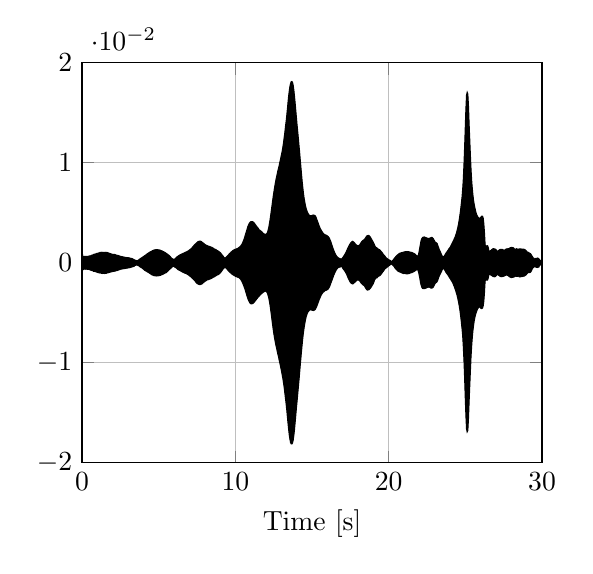
\begin{tikzpicture}

\begin{axis}[%
width=2.3in,
height=2in,
at={(0.758in,0.481in)},
scale only axis,
xmin=0,
xmax=30,
xmajorgrids,
ymin=-0.02,
ymax=0.02,
ymajorgrids,
xlabel={Time [s]},
axis background/.style={fill=white}
]
\addplot[fill=black,draw=black,forget plot] plot table[row sep=crcr]{%
2.08333333333333e-05	0.00127804279327393\\
0.0417454218822439	0.000631213188171387\\
0.0834700104311544	0.000625014305114746\\
0.125194598980065	0.000635147094726563\\
0.166919187528975	0.000628471374511719\\
0.208643776077886	0.000626802444458008\\
0.250368364626797	0.000621795654296875\\
0.292092953175707	0.000622868537902832\\
0.333817541724618	0.000628829002380371\\
0.375542130273528	0.000621318817138672\\
0.417266718822439	0.000651001930236816\\
0.458991307371349	0.000663518905639648\\
0.50071589592026	0.000679612159729004\\
0.54244048446917	0.000688552856445313\\
0.584165073018081	0.000703096389770508\\
0.625889661566991	0.000748038291931152\\
0.667614250115902	0.000764727592468262\\
0.709338838664812	0.000782251358032227\\
0.751063427213723	0.000815749168395996\\
0.792788015762633	0.000848770141601563\\
0.834512604311544	0.000861644744873047\\
0.876237192860454	0.000872373580932617\\
0.917961781409365	0.000892996788024902\\
0.959686369958275	0.000927567481994629\\
1.00141095850719	0.00093841552734375\\
1.0431355470561	0.000953912734985352\\
1.08486013560501	0.000977635383605957\\
1.12658472415392	0.000986456871032715\\
1.16830931270283	0.00102269649505615\\
1.21003390125174	0.00102055072784424\\
1.25175848980065	0.00102221965789795\\
1.29348307834956	0.00104677677154541\\
1.33520766689847	0.00104153156280518\\
1.37693225544738	0.00103974342346191\\
1.41865684399629	0.00103652477264404\\
1.4603814325452	0.00104057788848877\\
1.50210602109411	0.00103223323822021\\
1.54383060964302	0.00104439258575439\\
1.58555519819193	0.00103390216827393\\
1.62727978674084	0.00102889537811279\\
1.66900437528975	0.000995635986328125\\
1.71072896383866	0.000981450080871582\\
1.75245355238758	0.000968337059020996\\
1.79417814093649	0.000933051109313965\\
1.8359027294854	0.000915884971618652\\
1.87762731803431	0.000895857810974121\\
1.91935190658322	0.000874638557434082\\
1.96107649513213	0.000847458839416504\\
2.00280108368104	0.000832915306091309\\
2.04452567222995	0.000840663909912109\\
2.08625026077886	0.000831246376037598\\
2.12797484932777	0.000821232795715332\\
2.16969943787668	0.000807404518127441\\
2.21142402642559	0.000768899917602539\\
2.2531486149745	0.000757694244384766\\
2.29487320352341	0.000733017921447754\\
2.33659779207232	0.000726103782653809\\
2.37832238062123	0.000716090202331543\\
2.42004696917014	0.000691056251525879\\
2.46177155771905	0.000661253929138184\\
2.50349614626796	0.000634193420410156\\
2.54522073481687	0.00062716007232666\\
2.58694532336579	0.000597119331359863\\
2.6286699119147	0.000601649284362793\\
2.67039450046361	0.000583291053771973\\
2.71211908901252	0.000567436218261719\\
2.75384367756143	0.000557541847229004\\
2.79556826611034	0.000541567802429199\\
2.83729285465925	0.000536680221557617\\
2.87901744320816	0.000523209571838379\\
2.92074203175707	0.000514030456542969\\
2.96246662030598	0.000505685806274414\\
3.00419120885489	0.000509381294250488\\
3.0459157974038	0.000492453575134277\\
3.08764038595271	0.000486135482788086\\
3.12936497450162	0.000458955764770508\\
3.17108956305053	0.000441431999206543\\
3.21281415159944	0.000431060791015625\\
3.25453874014835	0.000412344932556152\\
3.29626332869726	0.000388026237487793\\
3.33798791724618	0.000339627265930176\\
3.37971250579509	0.000316739082336426\\
3.421437094344	0.000280022621154785\\
3.46316168289291	0.000258326530456543\\
3.50488627144182	0.000225305557250977\\
3.54661085999073	0.000218987464904785\\
3.58833544853964	0.000194072723388672\\
3.63006003708855	0.000222444534301758\\
3.67178462563746	0.000257372856140137\\
3.71350921418637	0.000302910804748535\\
3.75523380273528	0.000357985496520996\\
3.79695839128419	0.000406026840209961\\
3.8386829798331	0.00044560432434082\\
3.88040756838201	0.000483155250549316\\
3.92213215693092	0.000528216361999512\\
3.96385674547983	0.000562429428100586\\
4.00558133402874	0.00061953067779541\\
4.04730592257765	0.000665068626403809\\
4.08903051112656	0.000702261924743652\\
4.13075509967547	0.000744342803955078\\
4.17247968822439	0.000792741775512695\\
4.2142042767733	0.0008544921875\\
4.25592886532221	0.000883221626281738\\
4.29765345387112	0.000934243202209473\\
4.33937804242003	0.000978946685791016\\
4.38110263096894	0.00101733207702637\\
4.42282721951785	0.00105810165405273\\
4.46455180806676	0.00109744071960449\\
4.50627639661567	0.00111865997314453\\
4.54800098516458	0.00115501880645752\\
4.58972557371349	0.00120365619659424\\
4.6314501622624	0.00122451782226563\\
4.67317475081131	0.00125038623809814\\
4.71489933936022	0.00128710269927979\\
4.75662392790913	0.00128340721130371\\
4.79834851645804	0.00130021572113037\\
4.84007310500695	0.00130677223205566\\
4.88179769355586	0.00130546092987061\\
4.92352228210478	0.00130975246429443\\
4.96524687065368	0.00129389762878418\\
5.0069714592026	0.00129055976867676\\
5.04869604775151	0.00127255916595459\\
5.09042063630042	0.00126254558563232\\
5.13214522484933	0.00122177600860596\\
5.17386981339824	0.00119674205780029\\
5.21559440194715	0.00117611885070801\\
5.25731899049606	0.00114655494689941\\
5.29904357904497	0.00110149383544922\\
5.34076816759388	0.00109362602233887\\
5.38249275614279	0.00103819370269775\\
5.4242173446917	0.00101065635681152\\
5.46594193324061	0.000965595245361328\\
5.50766652178952	0.000915408134460449\\
5.54939111033843	0.000874519348144531\\
5.59111569888734	0.000841140747070313\\
5.63284028743625	0.000781059265136719\\
5.67456487598516	0.000725507736206055\\
5.71628946453407	0.000658035278320313\\
5.75801405308299	0.000604987144470215\\
5.7997386416319	0.000518560409545898\\
5.84146323018081	0.000460147857666016\\
5.88318781872972	0.000397682189941406\\
5.92491240727863	0.00036311149597168\\
5.96663699582754	0.000349760055541992\\
6.00836158437645	0.000349640846252441\\
6.05008617292536	0.000375509262084961\\
6.09181076147427	0.000434398651123047\\
6.13353535002318	0.000504136085510254\\
6.17525993857209	0.000555276870727539\\
6.216984527121	0.00062251091003418\\
6.25870911566991	0.000640511512756348\\
6.30043370421882	0.000700473785400391\\
6.34215829276773	0.000741958618164063\\
6.38388288131664	0.000778675079345703\\
6.42560746986555	0.000809073448181152\\
6.46733205841446	0.000843644142150879\\
6.50905664696338	0.000872969627380371\\
6.55078123551229	0.00089871883392334\\
6.5925058240612	0.000939726829528809\\
6.63423041261011	0.000955104827880859\\
6.67595500115902	0.00098717212677002\\
6.71767958970793	0.00101554393768311\\
6.75940417825684	0.00105273723602295\\
6.80112876680575	0.00108933448791504\\
6.84285335535466	0.00110065937042236\\
6.88457794390357	0.00114583969116211\\
6.92630253245248	0.00117993354797363\\
6.96802712100139	0.00121629238128662\\
7.0097517095503	0.00127542018890381\\
7.05147629809921	0.00132966041564941\\
7.09320088664812	0.00136947631835938\\
7.13492547519703	0.0014340877532959\\
7.17665006374594	0.00149333477020264\\
7.21837465229485	0.00157928466796875\\
7.26009924084376	0.00163924694061279\\
7.30182382939268	0.00172519683837891\\
7.34354841794159	0.00178694725036621\\
7.3852730064905	0.00186848640441895\\
7.42699759503941	0.00191104412078857\\
7.46872218358832	0.00197887420654297\\
7.51044677213723	0.00203204154968262\\
7.55217136068614	0.00209450721740723\\
7.59389594923505	0.00211906433105469\\
7.63562053778396	0.0021517276763916\\
7.67734512633287	0.00215578079223633\\
7.71906971488178	0.00215423107147217\\
7.76079430343069	0.00213372707366943\\
7.8025188919796	0.0020899772644043\\
7.84424348052851	0.00203394889831543\\
7.88596806907742	0.00199556350708008\\
7.92769265762633	0.00193679332733154\\
7.96941724617524	0.00188601016998291\\
8.01114183472416	0.00183010101318359\\
8.05286642327307	0.00178492069244385\\
8.09459101182198	0.00175571441650391\\
8.13631560037089	0.00172579288482666\\
8.1780401889198	0.00169909000396729\\
8.21976477746871	0.00166606903076172\\
8.26148936601762	0.00164306163787842\\
8.30321395456653	0.00163936614990234\\
8.34493854311544	0.00160729885101318\\
8.38666313166435	0.00157511234283447\\
8.42838772021326	0.00156009197235107\\
8.47011230876217	0.0015329122543335\\
8.51183689731108	0.00149202346801758\\
8.55356148585999	0.0014570951461792\\
8.5952860744089	0.00141036510467529\\
8.63701066295781	0.00136888027191162\\
8.67873525150672	0.00133645534515381\\
8.72045984005563	0.00132477283477783\\
8.76218442860454	0.00127542018890381\\
8.80390901715345	0.00122463703155518\\
8.84563360570237	0.00119531154632568\\
8.88735819425128	0.0011591911315918\\
8.92908278280018	0.00110948085784912\\
8.9708073713491	0.00105977058410645\\
9.01253195989801	0.00100851058959961\\
9.05425654844692	0.000942230224609375\\
9.09598113699583	0.000854015350341797\\
9.13770572554474	0.000771164894104004\\
9.17943031409365	0.000705480575561523\\
9.22115490264256	0.000602602958679199\\
9.26287949119147	0.000526070594787598\\
9.30460407974038	0.000465273857116699\\
9.34632866828929	0.000481009483337402\\
9.3880532568382	0.000534534454345703\\
9.42977784538711	0.000605940818786621\\
9.47150243393602	0.000667691230773926\\
9.51322702248493	0.000735163688659668\\
9.55495161103384	0.000798940658569336\\
9.59667619958275	0.000867486000061035\\
9.63840078813166	0.000937104225158691\\
9.68012537668058	0.000984668731689453\\
9.72184996522949	0.00106942653656006\\
9.7635745537784	0.00111746788024902\\
9.80529914232731	0.00117456912994385\\
9.84702373087622	0.00122499465942383\\
9.88874831942513	0.00126338005065918\\
9.93047290797404	0.00129258632659912\\
9.97219749652295	0.00134050846099854\\
10.0139220850719	0.00134932994842529\\
10.0556466736208	0.00137102603912354\\
10.0973712621697	0.0014040470123291\\
10.1390958507186	0.00142395496368408\\
10.1808204392675	0.00145864486694336\\
10.2225450278164	0.00151920318603516\\
10.2642696163653	0.00155460834503174\\
10.3059942049142	0.00160431861877441\\
10.3477187934631	0.0016859769821167\\
10.3894433820121	0.00176119804382324\\
10.431167970561	0.00186002254486084\\
10.4728925591099	0.00198805332183838\\
10.5146171476588	0.00213873386383057\\
10.5563417362077	0.00231361389160156\\
10.5980663247566	0.00249052047729492\\
10.6397909133055	0.00271880626678467\\
10.6815155018544	0.0029449462890625\\
10.7232400904033	0.003135085105896\\
10.7649646789523	0.00335073471069336\\
10.8066892675012	0.00357913970947266\\
10.8484138560501	0.00374186038970947\\
10.890138444599	0.00388526916503906\\
10.9318630331479	0.00398504734039307\\
10.9735876216968	0.00407087802886963\\
11.0153122102457	0.00409936904907227\\
11.0570367987946	0.00411760807037354\\
11.0987613873435	0.00410938262939453\\
11.1404859758924	0.00409233570098877\\
11.1822105644414	0.00403416156768799\\
11.2239351529903	0.00398910045623779\\
11.2656597415392	0.00389575958251953\\
11.3073843300881	0.00380027294158936\\
11.349108918637	0.00370848178863525\\
11.3908335071859	0.0036165714263916\\
11.4325580957348	0.00354766845703125\\
11.4742826842837	0.00347673892974854\\
11.5160072728326	0.00337421894073486\\
11.5577318613816	0.00328707695007324\\
11.5994564499305	0.00325310230255127\\
11.6411810384794	0.0031893253326416\\
11.6829056270283	0.00314855575561523\\
11.7246302155772	0.00309467315673828\\
11.7663548041261	0.00300943851470947\\
11.808079392675	0.00295102596282959\\
11.8498039812239	0.0028998851776123\\
11.8915285697728	0.00287175178527832\\
11.9332531583217	0.00284099578857422\\
11.9749777468707	0.00283515453338623\\
12.0167023354196	0.0028756856918335\\
12.0584269239685	0.0029294490814209\\
12.1001515125174	0.00305366516113281\\
12.1418761010663	0.00328326225280762\\
12.1836006896152	0.003562331199646\\
12.2253252781641	0.00393486022949219\\
12.267049866713	0.00432932376861572\\
12.3087744552619	0.00478744506835938\\
12.3504990438108	0.00525879859924316\\
12.3922236323598	0.0057370662689209\\
12.4339482209087	0.00622677803039551\\
12.4756728094576	0.00669920444488525\\
12.5173973980065	0.00710928440093994\\
12.5591219865554	0.0075230598449707\\
12.6008465751043	0.00789737701416016\\
12.6425711636532	0.00824654102325439\\
12.6842957522021	0.00855863094329834\\
12.726020340751	0.00884735584259033\\
12.7677449293	0.00915205478668213\\
12.8094695178489	0.00941121578216553\\
12.8511941063978	0.00967514514923096\\
12.8929186949467	0.00999438762664795\\
12.9346432834956	0.0102517604827881\\
12.9763678720445	0.0105814933776855\\
13.0180924605934	0.0108782052993774\\
13.0598170491423	0.011201024055481\\
13.1015416376912	0.0115941762924194\\
13.1432662262401	0.012012243270874\\
13.1849908147891	0.0125203132629395\\
13.226715403338	0.0130273103713989\\
13.2684399918869	0.0136046409606934\\
13.3101645804358	0.0141032934188843\\
13.3518891689847	0.0147042274475098\\
13.3936137575336	0.0153554677963257\\
13.4353383460825	0.0160462856292725\\
13.4770629346314	0.0166767835617065\\
13.5187875231803	0.0172096490859985\\
13.5605121117293	0.0176523923873901\\
13.6022367002782	0.0179364681243896\\
13.6439612888271	0.0181000232696533\\
13.685685877376	0.0181249380111694\\
13.7274104659249	0.0180306434631348\\
13.7691350544738	0.0177460908889771\\
13.8108596430227	0.0172954797744751\\
13.8525842315716	0.0166802406311035\\
13.8943088201205	0.0160108804702759\\
13.9360334086694	0.0152887105941772\\
13.9777579972184	0.014556884765625\\
14.0194825857673	0.0138355493545532\\
14.0612071743162	0.0131707191467285\\
14.1029317628651	0.012508749961853\\
14.144656351414	0.0117968320846558\\
14.1863809399629	0.0111017227172852\\
14.2281055285118	0.0103411674499512\\
14.2698301170607	0.00961518287658691\\
14.3115547056096	0.00887918472290039\\
14.3532792941586	0.0081636905670166\\
14.3950038827075	0.00755643844604492\\
14.4367284712564	0.00697898864746094\\
14.4784530598053	0.00649642944335938\\
14.5201776483542	0.0061107873916626\\
14.5619022369031	0.00577616691589355\\
14.603626825452	0.00548958778381348\\
14.6453514140009	0.00526928901672363\\
14.6870760025498	0.00509107112884521\\
14.7288005910988	0.00496208667755127\\
14.7705251796477	0.00485360622406006\\
14.8122497681966	0.00475609302520752\\
14.8539743567455	0.00471067428588867\\
14.8956989452944	0.00469815731048584\\
14.9374235338433	0.00469648838043213\\
14.9791481223922	0.00470972061157227\\
15.0208727109411	0.00475072860717773\\
15.06259729949	0.00476610660552979\\
15.1043218880389	0.00477027893066406\\
15.1460464765879	0.00474727153778076\\
15.1877710651368	0.00470900535583496\\
15.2294956536857	0.0046459436416626\\
15.2712202422346	0.00450277328491211\\
15.3129448307835	0.00431835651397705\\
15.3546694193324	0.00414323806762695\\
15.3963940078813	0.00397789478302002\\
15.4381185964302	0.00377774238586426\\
15.4798431849791	0.00362992286682129\\
15.521567773528	0.00346171855926514\\
15.563292362077	0.00334203243255615\\
15.6050169506259	0.00322949886322021\\
15.6467415391748	0.00311958789825439\\
15.6884661277237	0.0030292272567749\\
15.7301907162726	0.00293910503387451\\
15.7719153048215	0.00287222862243652\\
15.8136398933704	0.00282394886016846\\
15.8553644819193	0.00278961658477783\\
15.8970890704682	0.00276505947113037\\
15.9388136590172	0.00274670124053955\\
15.9805382475661	0.00270199775695801\\
16.022262836115	0.00265073776245117\\
16.0639874246639	0.00259053707122803\\
16.1057120132128	0.00251424312591553\\
16.1474366017617	0.00238251686096191\\
16.1891611903106	0.00223147869110107\\
16.2308857788595	0.00208532810211182\\
16.2726103674084	0.0018693208694458\\
16.3143349559573	0.00169098377227783\\
16.3560595445063	0.00147318840026855\\
16.3977841330552	0.00132143497467041\\
16.4395087216041	0.00113749504089355\\
16.481233310153	0.00098264217376709\\
16.5229578987019	0.000874996185302734\\
16.5646824872508	0.000738620758056641\\
16.6064070757997	0.000650525093078613\\
16.6481316643486	0.00056755542755127\\
16.6898562528975	0.000516533851623535\\
16.7315808414465	0.000478267669677734\\
16.7733054299954	0.000433444976806641\\
16.8150300185443	0.000414729118347168\\
16.8567546070932	0.000384330749511719\\
16.8984791956421	0.00037682056427002\\
16.940203784191	0.000384211540222168\\
16.9819283727399	0.000468611717224121\\
17.0236529612888	0.00055539608001709\\
17.0653775498377	0.000656843185424805\\
17.1071021383867	0.000748038291931152\\
17.1488267269356	0.000851631164550781\\
17.1905513154845	0.000960946083068848\\
17.2322759040334	0.0010915994644165\\
17.2740004925823	0.00124549865722656\\
17.3157250811312	0.00138700008392334\\
17.3574496696801	0.0015188455581665\\
17.399174258229	0.00166404247283936\\
17.4408988467779	0.00178706645965576\\
17.4826234353268	0.0018768310546875\\
17.5243480238758	0.00198018550872803\\
17.5660726124247	0.00205063819885254\\
17.6077972009736	0.00211203098297119\\
17.6495217895225	0.00213837623596191\\
17.6912463780714	0.00209248065948486\\
17.7329709666203	0.00203239917755127\\
17.7746955551692	0.00196850299835205\\
17.8164201437181	0.00189638137817383\\
17.858144732267	0.00183045864105225\\
17.8998693208159	0.0017702579498291\\
17.9415939093649	0.00172531604766846\\
17.9833184979138	0.00170111656188965\\
18.0250430864627	0.0017085075378418\\
18.0667676750116	0.00173532962799072\\
18.1084922635605	0.00178778171539307\\
18.1502168521094	0.00189721584320068\\
18.1919414406583	0.00199604034423828\\
18.2336660292072	0.00208830833435059\\
18.2753906177561	0.00217342376708984\\
18.3171152063051	0.00222349166870117\\
18.358839794854	0.00226426124572754\\
18.4005643834029	0.00230693817138672\\
18.4422889719518	0.00237786769866943\\
18.4840135605007	0.00247800350189209\\
18.5257381490496	0.00257432460784912\\
18.5674627375985	0.0026702880859375\\
18.6091873261474	0.00271201133728027\\
18.6509119146963	0.00272214412689209\\
18.6926365032453	0.0027320384979248\\
18.7343610917942	0.00268161296844482\\
18.7760856803431	0.00261020660400391\\
18.817810268892	0.00252974033355713\\
18.8595348574409	0.00240576267242432\\
18.9012594459898	0.00229310989379883\\
18.9429840345387	0.00217711925506592\\
18.9847086230876	0.0020749568939209\\
19.0264332116365	0.00192344188690186\\
19.0681578001854	0.00179409980773926\\
19.1098823887344	0.00164484977722168\\
19.1516069772833	0.0015639066696167\\
19.1933315658322	0.00151050090789795\\
19.2350561543811	0.00147199630737305\\
19.27678074293	0.00143206119537354\\
19.3185053314789	0.00135934352874756\\
19.3602299200278	0.00132179260253906\\
19.4019545085767	0.00131142139434814\\
19.4436790971256	0.00124466419219971\\
19.4854036856745	0.00116324424743652\\
19.5271282742235	0.00109946727752686\\
19.5688528627724	0.00101351737976074\\
19.6105774513213	0.000917196273803711\\
19.6523020398702	0.000830292701721191\\
19.6940266284191	0.000766158103942871\\
19.735751216968	0.00069272518157959\\
19.7774758055169	0.000599980354309082\\
19.8192003940658	0.000518560409545898\\
19.8609249826147	0.000458955764770508\\
19.9026495711637	0.000408053398132324\\
19.9443741597126	0.000364780426025391\\
19.9860987482615	0.000320792198181152\\
20.0278233368104	0.000272393226623535\\
20.0695479253593	0.000250339508056641\\
20.1112725139082	0.000214934349060059\\
20.1529971024571	0.000171542167663574\\
20.194721691006	0.000146985054016113\\
20.2364462795549	0.000164389610290527\\
20.2781708681038	0.000265717506408691\\
20.3198954566528	0.000333309173583984\\
20.3616200452017	0.000410079956054688\\
20.4033446337506	0.000494480133056641\\
20.4450692222995	0.000574469566345215\\
20.4867938108484	0.000638842582702637\\
20.5285183993973	0.000702261924743652\\
20.5702429879462	0.000772714614868164\\
20.6119675764951	0.000812888145446777\\
20.653692165044	0.000873804092407227\\
20.695416753593	0.000924110412597656\\
20.7371413421419	0.000951766967773438\\
20.7788659306908	0.000968456268310547\\
20.8205905192397	0.00100481510162354\\
20.8623151077886	0.00101923942565918\\
20.9040396963375	0.00103354454040527\\
20.9457642848864	0.00104677677154541\\
20.9874888734353	0.00106978416442871\\
21.0292134619842	0.00108063220977783\\
21.0709380505331	0.00110197067260742\\
21.1126626390821	0.00110578536987305\\
21.154387227631	0.00111269950866699\\
21.1961118161799	0.0011211633682251\\
21.2378364047288	0.00109267234802246\\
21.2795609932777	0.00110900402069092\\
21.3212855818266	0.0010993480682373\\
21.3630101703755	0.00107061862945557\\
21.4047347589244	0.00106143951416016\\
21.4464593474733	0.00103640556335449\\
21.4881839360223	0.00104343891143799\\
21.5299085245712	0.00100553035736084\\
21.5716331131201	0.000985622406005859\\
21.613357701669	0.000940918922424316\\
21.6550822902179	0.000916361808776855\\
21.6968068787668	0.000889897346496582\\
21.7385314673157	0.000823616981506348\\
21.7802560558646	0.000762343406677246\\
21.8219806444135	0.000701904296875\\
21.8637052329624	0.000655055046081543\\
21.9054298215114	0.000687241554260254\\
21.9471544100603	0.000838160514831543\\
21.9888789986092	0.00113999843597412\\
22.0306035871581	0.00152075290679932\\
22.072328175707	0.00187468528747559\\
22.1140527642559	0.00221681594848633\\
22.1557773528048	0.00239455699920654\\
22.1975019413537	0.00249767303466797\\
22.2392265299026	0.00254964828491211\\
22.2809511184516	0.00256383419036865\\
22.3226757070005	0.00257682800292969\\
22.3644002955494	0.00254476070404053\\
22.4061248840983	0.00252056121826172\\
22.4478494726472	0.00248932838439941\\
22.4895740611961	0.00247585773468018\\
22.531298649745	0.00244200229644775\\
22.5730232382939	0.00242948532104492\\
22.6147478268428	0.00242924690246582\\
22.6564724153917	0.00244510173797607\\
22.6981970039407	0.00247335433959961\\
22.7399215924896	0.00249636173248291\\
22.7816461810385	0.00252437591552734\\
22.8233707695874	0.00253105163574219\\
22.8650953581363	0.00247752666473389\\
22.9068199466852	0.00240111351013184\\
22.9485445352341	0.00229179859161377\\
22.990269123783	0.00217175483703613\\
23.0319937123319	0.00206196308135986\\
23.0737183008809	0.00201737880706787\\
23.1154428894298	0.00197815895080566\\
23.1571674779787	0.001914381980896\\
23.1988920665276	0.00174415111541748\\
23.2406166550765	0.00155723094940186\\
23.2823412436254	0.00137650966644287\\
23.3240658321743	0.00122785568237305\\
23.3657904207232	0.0011066198348999\\
23.4075150092721	0.000943422317504883\\
23.449239597821	0.000793099403381348\\
23.49096418637	0.000658512115478516\\
23.5326887749189	0.000577569007873535\\
23.5744133634678	0.000577449798583984\\
23.6161379520167	0.000663876533508301\\
23.6578625405656	0.000740528106689453\\
23.6995871291145	0.000880002975463867\\
23.7413117176634	0.00096583366394043\\
23.7830363062123	0.00106024742126465\\
23.8247608947612	0.00114238262176514\\
23.8664854833102	0.00124049186706543\\
23.9082100718591	0.00134313106536865\\
23.949934660408	0.00144410133361816\\
23.9916592489569	0.00151205062866211\\
24.0333838375058	0.00162482261657715\\
24.0751084260547	0.00174117088317871\\
24.1168330146036	0.00186669826507568\\
24.1585576031525	0.00199449062347412\\
24.2002821917014	0.00214552879333496\\
24.2420067802503	0.00225734710693359\\
24.2837313687993	0.00240910053253174\\
24.3254559573482	0.00255143642425537\\
24.3671805458971	0.00274038314819336\\
24.408905134446	0.0029289722442627\\
24.4506297229949	0.00315427780151367\\
24.4923543115438	0.00340795516967773\\
24.5340789000927	0.00371301174163818\\
24.5758034886416	0.00405347347259521\\
24.6175280771905	0.004477858543396\\
24.6592526657395	0.00492167472839355\\
24.7009772542884	0.00541150569915771\\
24.7427018428373	0.0059894323348999\\
24.7844264313862	0.00655853748321533\\
24.8261510199351	0.007362961769104\\
24.867875608484	0.00837421417236328\\
24.9096001970329	0.00980007648468018\\
24.9513247855818	0.0114856958389282\\
24.9930493741307	0.0134135484695435\\
25.0347739626796	0.0153409242630005\\
25.0764985512286	0.0167388916015625\\
25.1182231397775	0.0170340538024902\\
25.1599477283264	0.0168673992156982\\
25.2016723168753	0.0156699419021606\\
25.2433969054242	0.0138726234436035\\
25.2851214939731	0.0123008489608765\\
25.326846082522	0.0107371807098389\\
25.3685706710709	0.00932610034942627\\
25.4102952596198	0.00820529460906982\\
25.4520198481687	0.00739765167236328\\
25.4937444367177	0.00674927234649658\\
25.5354690252666	0.00620806217193604\\
25.5771936138155	0.0058283805847168\\
25.6189182023644	0.00549626350402832\\
25.6606427909133	0.00521326065063477\\
25.7023673794622	0.00496041774749756\\
25.7440919680111	0.00478363037109375\\
25.78581655656	0.00464761257171631\\
25.8275411451089	0.0045546293258667\\
25.8692657336579	0.00447988510131836\\
25.9109903222068	0.00443220138549805\\
25.9527149107557	0.00445985794067383\\
25.9944394993046	0.00450396537780762\\
26.0361640878535	0.00461125373840332\\
26.0778886764024	0.00466263294219971\\
26.1196132649513	0.00464582443237305\\
26.1613378535002	0.00447726249694824\\
26.2030624420491	0.0039064884185791\\
26.2447870305981	0.00300025939941406\\
26.286511619147	0.00182676315307617\\
26.3282362076959	0.00153994560241699\\
26.3699607962448	0.00165724754333496\\
26.4116853847937	0.00171065330505371\\
26.4534099733426	0.00168359279632568\\
26.4951345618915	0.00149905681610107\\
26.5368591504404	0.00116610527038574\\
26.5785837389893	0.00111997127532959\\
26.6203083275383	0.00118911266326904\\
26.6620329160872	0.0012211799621582\\
26.7037575046361	0.00127851963043213\\
26.745482093185	0.00134193897247314\\
26.7872066817339	0.00138437747955322\\
26.8289312702828	0.00141060352325439\\
26.8706558588317	0.00138974189758301\\
26.9123804473806	0.00137734413146973\\
26.9541050359295	0.00135815143585205\\
26.9958296244784	0.00130808353424072\\
27.0375542130274	0.00120711326599121\\
27.0792788015763	0.00111997127532959\\
27.1210033901252	0.00116991996765137\\
27.1627279786741	0.00122678279876709\\
27.204452567223	0.00126850605010986\\
27.2461771557719	0.0013127326965332\\
27.2879017443208	0.00134360790252686\\
27.3296263328697	0.00133943557739258\\
27.3713509214186	0.00133466720581055\\
27.4130755099675	0.00132310390472412\\
27.4548000985165	0.0012892484664917\\
27.4965246870654	0.00125885009765625\\
27.5382492756143	0.00125181674957275\\
27.5799738641632	0.00126266479492188\\
27.6216984527121	0.00133514404296875\\
27.663423041261	0.00136935710906982\\
27.7051476298099	0.00139367580413818\\
27.7468722183588	0.00139355659484863\\
27.7885968069077	0.00139641761779785\\
27.8303213954567	0.00139939785003662\\
27.8720459840056	0.0014498233795166\\
27.9137705725545	0.0014873743057251\\
27.9554951611034	0.00151157379150391\\
27.9972197496523	0.00152623653411865\\
28.0389443382012	0.00152468681335449\\
28.0806689267501	0.00151371955871582\\
28.122393515299	0.00149452686309814\\
28.1641181038479	0.00145208835601807\\
28.2058426923968	0.00135600566864014\\
28.2475672809458	0.00132095813751221\\
28.2892918694947	0.00136649608612061\\
28.3310164580436	0.00140035152435303\\
28.3727410465925	0.0013735294342041\\
28.4144656351414	0.00135397911071777\\
28.4561902236903	0.0013434886932373\\
28.4979148122392	0.00136935710906982\\
28.5396394007881	0.00138866901397705\\
28.581363989337	0.00139319896697998\\
28.623088577886	0.00137901306152344\\
28.6648131664349	0.00135350227355957\\
28.7065377549838	0.00134694576263428\\
28.7482623435327	0.0013422966003418\\
28.7899869320816	0.00135385990142822\\
28.8317115206305	0.00134527683258057\\
28.8734361091794	0.00130677223205566\\
28.9151606977283	0.0012671947479248\\
28.9568852862772	0.00120365619659424\\
28.9986098748261	0.00113034248352051\\
29.0403344633751	0.00106322765350342\\
29.082059051924	0.00106358528137207\\
29.1237836404729	0.00101351737976074\\
29.1655082290218	0.000969767570495605\\
29.2072328175707	0.000931739807128906\\
29.2489574061196	0.000900745391845703\\
29.2906819946685	0.000811934471130371\\
29.3324065832174	0.000694751739501953\\
29.3741311717663	0.000607967376708984\\
29.4158557603153	0.000501155853271484\\
29.4575803488642	0.000453591346740723\\
29.4993049374131	0.000370621681213379\\
29.541029525962	0.000379204750061035\\
29.5827541145109	0.000430107116699219\\
29.6244787030598	0.00041806697845459\\
29.6662032916087	0.000442385673522949\\
29.7079278801576	0.000470161437988281\\
29.7496524687065	0.000450968742370605\\
29.7913770572554	0.000368475914001465\\
29.8331016458044	0.000347614288330078\\
29.8748262343533	0.000216484069824219\\
29.9165508229022	0.000200271606445313\\
29.9582754114511	0.000146865844726563\\
30	0.000100493431091309\\
}
\closedcycle;
\addplot[fill=black,draw=black,forget plot] plot table[row sep=crcr]{%
2.08333333333333e-05	-0.00102686882019043\\
0.0417454218822439	-0.000666379928588867\\
0.0834700104311544	-0.000653386116027832\\
0.125194598980065	-0.000644683837890625\\
0.166919187528975	-0.000635027885437012\\
0.208643776077886	-0.000647187232971191\\
0.250368364626797	-0.000632405281066895\\
0.292092953175707	-0.00063621997833252\\
0.333817541724618	-0.000647187232971191\\
0.375542130273528	-0.000648021697998047\\
0.417266718822439	-0.000648260116577148\\
0.458991307371349	-0.000664114952087402\\
0.50071589592026	-0.00068211555480957\\
0.54244048446917	-0.000726819038391113\\
0.584165073018081	-0.000746726989746094\\
0.625889661566991	-0.00075685977935791\\
0.667614250115902	-0.000790715217590332\\
0.709338838664812	-0.00079190731048584\\
0.751063427213723	-0.000853300094604492\\
0.792788015762633	-0.000846028327941895\\
0.834512604311544	-0.000860214233398438\\
0.876237192860454	-0.000890254974365234\\
0.917961781409365	-0.000910758972167969\\
0.959686369958275	-0.000927567481994629\\
1.00141095850719	-0.000959515571594238\\
1.0431355470561	-0.000976800918579102\\
1.08486013560501	-0.000985383987426758\\
1.12658472415392	-0.00101625919342041\\
1.16830931270283	-0.00102126598358154\\
1.21003390125174	-0.00101637840270996\\
1.25175848980065	-0.00104856491088867\\
1.29348307834956	-0.00104689598083496\\
1.33520766689847	-0.00107026100158691\\
1.37693225544738	-0.00106298923492432\\
1.41865684399629	-0.00106143951416016\\
1.4603814325452	-0.0010751485824585\\
1.50210602109411	-0.00105762481689453\\
1.54383060964302	-0.00104224681854248\\
1.58555519819193	-0.00104773044586182\\
1.62727978674084	-0.00101590156555176\\
1.66900437528975	-0.00101542472839355\\
1.71072896383866	-0.000998497009277344\\
1.75245355238758	-0.000977516174316406\\
1.79417814093649	-0.000947475433349609\\
1.8359027294854	-0.000937104225158691\\
1.87762731803431	-0.000921726226806641\\
1.91935190658322	-0.000900387763977051\\
1.96107649513213	-0.000885844230651855\\
2.00280108368104	-0.000869870185852051\\
2.04452567222995	-0.000851869583129883\\
2.08625026077886	-0.000850319862365723\\
2.12797484932777	-0.000836014747619629\\
2.16969943787668	-0.000826478004455566\\
2.21142402642559	-0.000801920890808105\\
2.2531486149745	-0.000780701637268066\\
2.29487320352341	-0.000770926475524902\\
2.33659779207232	-0.00075066089630127\\
2.37832238062123	-0.000723123550415039\\
2.42004696917014	-0.000699996948242188\\
2.46177155771905	-0.000677227973937988\\
2.50349614626796	-0.000650525093078613\\
2.54522073481687	-0.000636696815490723\\
2.58694532336579	-0.000627517700195313\\
2.6286699119147	-0.000609159469604492\\
2.67039450046361	-0.000603795051574707\\
2.71211908901252	-0.000569581985473633\\
2.75384367756143	-0.000574469566345215\\
2.79556826611034	-0.000577807426452637\\
2.83729285465925	-0.000553607940673828\\
2.87901744320816	-0.000548124313354492\\
2.92074203175707	-0.00053560733795166\\
2.96246662030598	-0.000534415245056152\\
3.00419120885489	-0.000509023666381836\\
3.0459157974038	-0.000513076782226563\\
3.08764038595271	-0.000487208366394043\\
3.12936497450162	-0.000481367111206055\\
3.17108956305053	-0.000455498695373535\\
3.21281415159944	-0.000430583953857422\\
3.25453874014835	-0.00042271614074707\\
3.29626332869726	-0.000396370887756348\\
3.33798791724618	-0.000377535820007324\\
3.37971250579509	-0.0003662109375\\
3.421437094344	-0.000309467315673828\\
3.46316168289291	-0.000249028205871582\\
3.50488627144182	-0.000252366065979004\\
3.54661085999073	-0.000213146209716797\\
3.58833544853964	-0.000223159790039063\\
3.63006003708855	-0.000251650810241699\\
3.67178462563746	-0.000289201736450195\\
3.71350921418637	-0.000321149826049805\\
3.75523380273528	-0.000371217727661133\\
3.79695839128419	-0.000423431396484375\\
3.8386829798331	-0.000450491905212402\\
3.88040756838201	-0.000500679016113281\\
3.92213215693092	-0.000526070594787598\\
3.96385674547983	-0.000599026679992676\\
4.00558133402874	-0.000629186630249023\\
4.04730592257765	-0.000687122344970703\\
4.08903051112656	-0.000753521919250488\\
4.13075509967547	-0.000774025917053223\\
4.17247968822439	-0.000826478004455566\\
4.2142042767733	-0.000853180885314941\\
4.25592886532221	-0.00090491771697998\\
4.29765345387112	-0.000939130783081055\\
4.33937804242003	-0.000977635383605957\\
4.38110263096894	-0.00102019309997559\\
4.42282721951785	-0.00105965137481689\\
4.46455180806676	-0.00110352039337158\\
4.50627639661567	-0.00114989280700684\\
4.54800098516458	-0.00119566917419434\\
4.58972557371349	-0.0012061595916748\\
4.6314501622624	-0.00124907493591309\\
4.67317475081131	-0.00127971172332764\\
4.71489933936022	-0.00128829479217529\\
4.75662392790913	-0.00130546092987061\\
4.79834851645804	-0.00131499767303467\\
4.84007310500695	-0.00132215023040771\\
4.88179769355586	-0.00130057334899902\\
4.92352228210478	-0.00131082534790039\\
4.96524687065368	-0.00129926204681396\\
5.0069714592026	-0.00129044055938721\\
5.04869604775151	-0.00127971172332764\\
5.09042063630042	-0.00125789642333984\\
5.13214522484933	-0.00124466419219971\\
5.17386981339824	-0.00120401382446289\\
5.21559440194715	-0.00118374824523926\\
5.25731899049606	-0.0011669397354126\\
5.29904357904497	-0.0011293888092041\\
5.34076816759388	-0.00109195709228516\\
5.38249275614279	-0.00105810165405273\\
5.4242173446917	-0.00101017951965332\\
5.46594193324061	-0.00100290775299072\\
5.50766652178952	-0.000959157943725586\\
5.54939111033843	-0.000900030136108398\\
5.59111569888734	-0.00082850456237793\\
5.63284028743625	-0.000783085823059082\\
5.67456487598516	-0.000710010528564453\\
5.71628946453407	-0.000656366348266602\\
5.75801405308299	-0.000581622123718262\\
5.7997386416319	-0.000542402267456055\\
5.84146323018081	-0.000481128692626953\\
5.88318781872972	-0.000410914421081543\\
5.92491240727863	-0.000372648239135742\\
5.96663699582754	-0.000348806381225586\\
6.00836158437645	-0.000376343727111816\\
6.05008617292536	-0.000430464744567871\\
6.09181076147427	-0.000473618507385254\\
6.13353535002318	-0.000502347946166992\\
6.17525993857209	-0.000564455986022949\\
6.216984527121	-0.000625014305114746\\
6.25870911566991	-0.000676631927490234\\
6.30043370421882	-0.000699639320373535\\
6.34215829276773	-0.000757694244384766\\
6.38388288131664	-0.000777363777160645\\
6.42560746986555	-0.000813961029052734\\
6.46733205841446	-0.000852704048156738\\
6.50905664696338	-0.000889062881469727\\
6.55078123551229	-0.000915408134460449\\
6.5925058240612	-0.000960111618041992\\
6.63423041261011	-0.000981688499450684\\
6.67595500115902	-0.00102221965789795\\
6.71767958970793	-0.00103962421417236\\
6.75940417825684	-0.00105226039886475\\
6.80112876680575	-0.00108051300048828\\
6.84285335535466	-0.0011293888092041\\
6.88457794390357	-0.00115787982940674\\
6.92630253245248	-0.00120365619659424\\
6.96802712100139	-0.00123465061187744\\
7.0097517095503	-0.00132298469543457\\
7.05147629809921	-0.00133895874023438\\
7.09320088664812	-0.00139808654785156\\
7.13492547519703	-0.00146734714508057\\
7.17665006374594	-0.00152826309204102\\
7.21837465229485	-0.00159013271331787\\
7.26009924084376	-0.00165772438049316\\
7.30182382939268	-0.00171029567718506\\
7.34354841794159	-0.00177621841430664\\
7.3852730064905	-0.00184571743011475\\
7.42699759503941	-0.00194466114044189\\
7.46872218358832	-0.00201141834259033\\
7.51044677213723	-0.00208449363708496\\
7.55217136068614	-0.00210273265838623\\
7.59389594923505	-0.00214827060699463\\
7.63562053778396	-0.00216960906982422\\
7.67734512633287	-0.00217247009277344\\
7.71906971488178	-0.00217461585998535\\
7.76079430343069	-0.00214338302612305\\
7.8025188919796	-0.00213456153869629\\
7.84424348052851	-0.00208151340484619\\
7.88596806907742	-0.0020064115524292\\
7.92769265762633	-0.00198805332183838\\
7.96941724617524	-0.00190746784210205\\
8.01114183472416	-0.001861572265625\\
8.05286642327307	-0.00181961059570313\\
8.09459101182198	-0.0017857551574707\\
8.13631560037089	-0.00172650814056396\\
8.1780401889198	-0.00170445442199707\\
8.21976477746871	-0.00169551372528076\\
8.26148936601762	-0.0016704797744751\\
8.30321395456653	-0.00164508819580078\\
8.34493854311544	-0.00162088871002197\\
8.38666313166435	-0.00159966945648193\\
8.42838772021326	-0.0015636682510376\\
8.47011230876217	-0.00154459476470947\\
8.51183689731108	-0.00148701667785645\\
8.55356148585999	-0.00144493579864502\\
8.5952860744089	-0.00142264366149902\\
8.63701066295781	-0.0013965368270874\\
8.67873525150672	-0.00135350227355957\\
8.72045984005563	-0.00130546092987061\\
8.76218442860454	-0.00127053260803223\\
8.80390901715345	-0.00122749805450439\\
8.84563360570237	-0.00120830535888672\\
8.88735819425128	-0.00117897987365723\\
8.92908278280018	-0.00112974643707275\\
8.9708073713491	-0.00106942653656006\\
9.01253195989801	-0.00101053714752197\\
9.05425654844692	-0.000937938690185547\\
9.09598113699583	-0.000859379768371582\\
9.13770572554474	-0.000759363174438477\\
9.17943031409365	-0.000664949417114258\\
9.22115490264256	-0.000597000122070313\\
9.26287949119147	-0.000516057014465332\\
9.30460407974038	-0.000488877296447754\\
9.34632866828929	-0.000477790832519531\\
9.3880532568382	-0.00052487850189209\\
9.42977784538711	-0.000580787658691406\\
9.47150243393602	-0.000658869743347168\\
9.51322702248493	-0.000737667083740234\\
9.55495161103384	-0.000813484191894531\\
9.59667619958275	-0.000867843627929688\\
9.63840078813166	-0.000938653945922852\\
9.68012537668058	-0.00100386142730713\\
9.72184996522949	-0.00104475021362305\\
9.7635745537784	-0.00110816955566406\\
9.80529914232731	-0.00116312503814697\\
9.84702373087622	-0.00120985507965088\\
9.88874831942513	-0.00123989582061768\\
9.93047290797404	-0.00128579139709473\\
9.97219749652295	-0.00131833553314209\\
10.0139220850719	-0.00136172771453857\\
10.0556466736208	-0.001381516456604\\
10.0973712621697	-0.00140893459320068\\
10.1390958507186	-0.00143063068389893\\
10.1808204392675	-0.00146198272705078\\
10.2225450278164	-0.00147771835327148\\
10.2642696163653	-0.00153529644012451\\
10.3059942049142	-0.00158870220184326\\
10.3477187934631	-0.00164937973022461\\
10.3894433820121	-0.00176060199737549\\
10.431167970561	-0.00187122821807861\\
10.4728925591099	-0.00200474262237549\\
10.5146171476588	-0.0021744966506958\\
10.5563417362077	-0.00232183933258057\\
10.5980663247566	-0.00251173973083496\\
10.6397909133055	-0.00269830226898193\\
10.6815155018544	-0.0029139518737793\\
10.7232400904033	-0.00313377380371094\\
10.7649646789523	-0.00334537029266357\\
10.8066892675012	-0.00353193283081055\\
10.8484138560501	-0.00371968746185303\\
10.890138444599	-0.00384938716888428\\
10.9318630331479	-0.00397193431854248\\
10.9735876216968	-0.00406181812286377\\
11.0153122102457	-0.00410020351409912\\
11.0570367987946	-0.00410759449005127\\
11.0987613873435	-0.00409090518951416\\
11.1404859758924	-0.00406622886657715\\
11.1822105644414	-0.00400960445404053\\
11.2239351529903	-0.00394916534423828\\
11.2656597415392	-0.00386857986450195\\
11.3073843300881	-0.00379002094268799\\
11.349108918637	-0.00370407104492188\\
11.3908335071859	-0.0036236047744751\\
11.4325580957348	-0.00354516506195068\\
11.4742826842837	-0.00344586372375488\\
11.5160072728326	-0.00338876247406006\\
11.5577318613816	-0.00332152843475342\\
11.5994564499305	-0.00323891639709473\\
11.6411810384794	-0.00317728519439697\\
11.6829056270283	-0.00312745571136475\\
11.7246302155772	-0.00306165218353271\\
11.7663548041261	-0.00301694869995117\\
11.808079392675	-0.00295853614807129\\
11.8498039812239	-0.00291883945465088\\
11.8915285697728	-0.00288307666778564\\
11.9332531583217	-0.00284183025360107\\
11.9749777468707	-0.00283873081207275\\
12.0167023354196	-0.0028759241104126\\
12.0584269239685	-0.00294196605682373\\
12.1001515125174	-0.00307118892669678\\
12.1418761010663	-0.00330114364624023\\
12.1836006896152	-0.00355470180511475\\
12.2253252781641	-0.0038834810256958\\
12.267049866713	-0.00428617000579834\\
12.3087744552619	-0.00474965572357178\\
12.3504990438108	-0.00524497032165527\\
12.3922236323598	-0.00576281547546387\\
12.4339482209087	-0.00625550746917725\\
12.4756728094576	-0.00673317909240723\\
12.5173973980065	-0.00715768337249756\\
12.5591219865554	-0.00754010677337646\\
12.6008465751043	-0.00790107250213623\\
12.6425711636532	-0.00821995735168457\\
12.6842957522021	-0.00850951671600342\\
12.726020340751	-0.0088123083114624\\
12.7677449293	-0.00910806655883789\\
12.8094695178489	-0.00936484336853027\\
12.8511941063978	-0.00968718528747559\\
12.8929186949467	-0.00997006893157959\\
12.9346432834956	-0.0102742910385132\\
12.9763678720445	-0.0105773210525513\\
13.0180924605934	-0.0108996629714966\\
13.0598170491423	-0.0112502574920654\\
13.1015416376912	-0.01160728931427\\
13.1432662262401	-0.0120183229446411\\
13.1849908147891	-0.0124727487564087\\
13.226715403338	-0.0130163431167603\\
13.2684399918869	-0.0135517120361328\\
13.3101645804358	-0.0140920877456665\\
13.3518891689847	-0.0147049427032471\\
13.3936137575336	-0.015393853187561\\
13.4353383460825	-0.0160497426986694\\
13.4770629346314	-0.0166763067245483\\
13.5187875231803	-0.0172429084777832\\
13.5605121117293	-0.0176646709442139\\
13.6022367002782	-0.0179964303970337\\
13.6439612888271	-0.0181025266647339\\
13.685685877376	-0.0181208848953247\\
13.7274104659249	-0.0180073976516724\\
13.7691350544738	-0.0177512168884277\\
13.8108596430227	-0.0172833204269409\\
13.8525842315716	-0.0167142152786255\\
13.8943088201205	-0.0160259008407593\\
13.9360334086694	-0.0153111219406128\\
13.9777579972184	-0.0145564079284668\\
14.0194825857673	-0.0138918161392212\\
14.0612071743162	-0.0131994485855103\\
14.1029317628651	-0.0124948024749756\\
14.144656351414	-0.0118026733398438\\
14.1863809399629	-0.0110608339309692\\
14.2281055285118	-0.0102913379669189\\
14.2698301170607	-0.00957334041595459\\
14.3115547056096	-0.00885105133056641\\
14.3532792941586	-0.00818479061126709\\
14.3950038827075	-0.00755143165588379\\
14.4367284712564	-0.00699448585510254\\
14.4784530598053	-0.00654089450836182\\
14.5201776483542	-0.00613236427307129\\
14.5619022369031	-0.00577831268310547\\
14.603626825452	-0.00547540187835693\\
14.6453514140009	-0.00524592399597168\\
14.6870760025498	-0.00506806373596191\\
14.7288005910988	-0.00493490695953369\\
14.7705251796477	-0.0048527717590332\\
14.8122497681966	-0.0047755241394043\\
14.8539743567455	-0.00472378730773926\\
14.8956989452944	-0.00470960140228271\\
14.9374235338433	-0.00470256805419922\\
14.9791481223922	-0.00472474098205566\\
15.0208727109411	-0.0047614574432373\\
15.06259729949	-0.00475442409515381\\
15.1043218880389	-0.00477850437164307\\
15.1460464765879	-0.00473713874816895\\
15.1877710651368	-0.00469934940338135\\
15.2294956536857	-0.00460624694824219\\
15.2712202422346	-0.00448441505432129\\
15.3129448307835	-0.00434470176696777\\
15.3546694193324	-0.00415968894958496\\
15.3963940078813	-0.0039752721786499\\
15.4381185964302	-0.00381553173065186\\
15.4798431849791	-0.00362873077392578\\
15.521567773528	-0.00350189208984375\\
15.563292362077	-0.0033419132232666\\
15.6050169506259	-0.00321304798126221\\
15.6467415391748	-0.00310659408569336\\
15.6884661277237	-0.00301206111907959\\
15.7301907162726	-0.00294554233551025\\
15.7719153048215	-0.00288808345794678\\
15.8136398933704	-0.00282883644104004\\
15.8553644819193	-0.00278174877166748\\
15.8970890704682	-0.00276446342468262\\
15.9388136590172	-0.00273656845092773\\
15.9805382475661	-0.00270187854766846\\
16.022262836115	-0.00267112255096436\\
16.0639874246639	-0.00259840488433838\\
16.1057120132128	-0.00248885154724121\\
16.1474366017617	-0.0023655891418457\\
16.1891611903106	-0.00220334529876709\\
16.2308857788595	-0.0020214319229126\\
16.2726103674084	-0.00185668468475342\\
16.3143349559573	-0.0016709566116333\\
16.3560595445063	-0.00150001049041748\\
16.3977841330552	-0.00131964683532715\\
16.4395087216041	-0.00116312503814697\\
16.481233310153	-0.00100541114807129\\
16.5229578987019	-0.000876545906066895\\
16.5646824872508	-0.000755071640014648\\
16.6064070757997	-0.000649929046630859\\
16.6481316643486	-0.00057375431060791\\
16.6898562528975	-0.000494003295898438\\
16.7315808414465	-0.000458002090454102\\
16.7733054299954	-0.000444769859313965\\
16.8150300185443	-0.000413894653320313\\
16.8567546070932	-0.000420093536376953\\
16.8984791956421	-0.000382900238037109\\
16.940203784191	-0.000389695167541504\\
16.9819283727399	-0.000459432601928711\\
17.0236529612888	-0.000594973564147949\\
17.0653775498377	-0.000681757926940918\\
17.1071021383867	-0.000756382942199707\\
17.1488267269356	-0.000852823257446289\\
17.1905513154845	-0.000967860221862793\\
17.2322759040334	-0.00107777118682861\\
17.2740004925823	-0.00120365619659424\\
17.3157250811312	-0.00137054920196533\\
17.3574496696801	-0.00152325630187988\\
17.399174258229	-0.00165390968322754\\
17.4408988467779	-0.00179398059844971\\
17.4826234353268	-0.00191211700439453\\
17.5243480238758	-0.0019909143447876\\
17.5660726124247	-0.00206565856933594\\
17.6077972009736	-0.00208783149719238\\
17.6495217895225	-0.00211584568023682\\
17.6912463780714	-0.00209248065948486\\
17.7329709666203	-0.00201404094696045\\
17.7746955551692	-0.00198054313659668\\
17.8164201437181	-0.00191128253936768\\
17.858144732267	-0.00185918807983398\\
17.8998693208159	-0.00178325176239014\\
17.9415939093649	-0.00173318386077881\\
17.9833184979138	-0.00171351432800293\\
18.0250430864627	-0.00172817707061768\\
18.0667676750116	-0.0017695426940918\\
18.1084922635605	-0.00180900096893311\\
18.1502168521094	-0.00190556049346924\\
18.1919414406583	-0.0019993782043457\\
18.2336660292072	-0.00206601619720459\\
18.2753906177561	-0.00214529037475586\\
18.3171152063051	-0.00221168994903564\\
18.358839794854	-0.00223875045776367\\
18.4005643834029	-0.00228679180145264\\
18.4422889719518	-0.00237953662872314\\
18.4840135605007	-0.00248706340789795\\
18.5257381490496	-0.00259757041931152\\
18.5674627375985	-0.00268280506134033\\
18.6091873261474	-0.00273168087005615\\
18.6509119146963	-0.0027158260345459\\
18.6926365032453	-0.002707839012146\\
18.7343610917942	-0.00265765190124512\\
18.7760856803431	-0.00260400772094727\\
18.817810268892	-0.00252294540405273\\
18.8595348574409	-0.00242817401885986\\
18.9012594459898	-0.00231552124023438\\
18.9429840345387	-0.00220000743865967\\
18.9847086230876	-0.00211668014526367\\
19.0264332116365	-0.00194835662841797\\
19.0681578001854	-0.00175440311431885\\
19.1098823887344	-0.00164628028869629\\
19.1516069772833	-0.00155532360076904\\
19.1933315658322	-0.00151824951171875\\
19.2350561543811	-0.00150108337402344\\
19.27678074293	-0.00143194198608398\\
19.3185053314789	-0.00136184692382813\\
19.3602299200278	-0.00132215023040771\\
19.4019545085767	-0.00130808353424072\\
19.4436790971256	-0.00125670433044434\\
19.4854036856745	-0.00118029117584229\\
19.5271282742235	-0.00109553337097168\\
19.5688528627724	-0.00100457668304443\\
19.6105774513213	-0.000917792320251465\\
19.6523020398702	-0.000836491584777832\\
19.6940266284191	-0.000740885734558105\\
19.735751216968	-0.000651717185974121\\
19.7774758055169	-0.000586986541748047\\
19.8192003940658	-0.000533699989318848\\
19.8609249826147	-0.00048220157623291\\
19.9026495711637	-0.000432610511779785\\
19.9443741597126	-0.000380873680114746\\
19.9860987482615	-0.000327825546264648\\
20.0278233368104	-0.000278592109680176\\
20.0695479253593	-0.000237464904785156\\
20.1112725139082	-0.000184059143066406\\
20.1529971024571	-0.000144839286804199\\
20.194721691006	-0.00013887882232666\\
20.2364462795549	-0.000188946723937988\\
20.2781708681038	-0.000261187553405762\\
20.3198954566528	-0.000313401222229004\\
20.3616200452017	-0.000394344329833984\\
20.4033446337506	-0.000508546829223633\\
20.4450692222995	-0.000592947006225586\\
20.4867938108484	-0.000642895698547363\\
20.5285183993973	-0.000728368759155273\\
20.5702429879462	-0.000771880149841309\\
20.6119675764951	-0.000850796699523926\\
20.653692165044	-0.00088191032409668\\
20.695416753593	-0.000892758369445801\\
20.7371413421419	-0.000933647155761719\\
20.7788659306908	-0.000953435897827148\\
20.8205905192397	-0.000988483428955078\\
20.8623151077886	-0.0010145902633667\\
20.9040396963375	-0.00104022026062012\\
20.9457642848864	-0.00106632709503174\\
20.9874888734353	-0.00107467174530029\\
21.0292134619842	-0.0010676383972168\\
21.0709380505331	-0.00106465816497803\\
21.1126626390821	-0.00108933448791504\\
21.154387227631	-0.00110650062561035\\
21.1961118161799	-0.00109982490539551\\
21.2378364047288	-0.00110471248626709\\
21.2795609932777	-0.00109100341796875\\
21.3212855818266	-0.00106394290924072\\
21.3630101703755	-0.0010688304901123\\
21.4047347589244	-0.00102138519287109\\
21.4464593474733	-0.00100922584533691\\
21.4881839360223	-0.000975966453552246\\
21.5299085245712	-0.000971794128417969\\
21.5716331131201	-0.000926733016967773\\
21.613357701669	-0.000908374786376953\\
21.6550822902179	-0.00086522102355957\\
21.6968068787668	-0.00082695484161377\\
21.7385314673157	-0.000791549682617188\\
21.7802560558646	-0.000738024711608887\\
21.8219806444135	-0.000700831413269043\\
21.8637052329624	-0.000674962997436523\\
21.9054298215114	-0.000738024711608887\\
21.9471544100603	-0.000934123992919922\\
21.9888789986092	-0.00121963024139404\\
22.0306035871581	-0.00156295299530029\\
22.072328175707	-0.0019451379776001\\
22.1140527642559	-0.00223135948181152\\
22.1557773528048	-0.00242960453033447\\
22.1975019413537	-0.00254714488983154\\
22.2392265299026	-0.00258767604827881\\
22.2809511184516	-0.00258350372314453\\
22.3226757070005	-0.00258517265319824\\
22.3644002955494	-0.00257229804992676\\
22.4061248840983	-0.00254559516906738\\
22.4478494726472	-0.00252056121826172\\
22.4895740611961	-0.00249218940734863\\
22.531298649745	-0.00246202945709229\\
22.5730232382939	-0.00244569778442383\\
22.6147478268428	-0.00242829322814941\\
22.6564724153917	-0.00243496894836426\\
22.6981970039407	-0.00247800350189209\\
22.7399215924896	-0.0025172233581543\\
22.7816461810385	-0.00253641605377197\\
22.8233707695874	-0.00252556800842285\\
22.8650953581363	-0.00249457359313965\\
22.9068199466852	-0.00242948532104492\\
22.9485445352341	-0.00230026245117188\\
22.990269123783	-0.00216913223266602\\
23.0319937123319	-0.00205314159393311\\
23.0737183008809	-0.00199222564697266\\
23.1154428894298	-0.0019606351852417\\
23.1571674779787	-0.00188219547271729\\
23.1988920665276	-0.00173723697662354\\
23.2406166550765	-0.00152873992919922\\
23.2823412436254	-0.00137233734130859\\
23.3240658321743	-0.00122034549713135\\
23.3657904207232	-0.00111556053161621\\
23.4075150092721	-0.000976324081420898\\
23.449239597821	-0.000846624374389648\\
23.49096418637	-0.000690579414367676\\
23.5326887749189	-0.000537276268005371\\
23.5744133634678	-0.000586152076721191\\
23.6161379520167	-0.000647425651550293\\
23.6578625405656	-0.000736832618713379\\
23.6995871291145	-0.000848531723022461\\
23.7413117176634	-0.000972986221313477\\
23.7830363062123	-0.00105476379394531\\
23.8247608947612	-0.00114238262176514\\
23.8664854833102	-0.00122380256652832\\
23.9082100718591	-0.00132465362548828\\
23.949934660408	-0.00144946575164795\\
23.9916592489569	-0.00153660774230957\\
24.0333838375058	-0.00163185596466064\\
24.0751084260547	-0.00174367427825928\\
24.1168330146036	-0.00184333324432373\\
24.1585576031525	-0.0019533634185791\\
24.2002821917014	-0.00207483768463135\\
24.2420067802503	-0.00225341320037842\\
24.2837313687993	-0.00240159034729004\\
24.3254559573482	-0.00259566307067871\\
24.3671805458971	-0.00275778770446777\\
24.408905134446	-0.00301456451416016\\
24.4506297229949	-0.00319564342498779\\
24.4923543115438	-0.00346171855926514\\
24.5340789000927	-0.00376307964324951\\
24.5758034886416	-0.00408387184143066\\
24.6175280771905	-0.00446271896362305\\
24.6592526657395	-0.00490331649780273\\
24.7009772542884	-0.00541973114013672\\
24.7427018428373	-0.00597596168518066\\
24.7844264313862	-0.00660145282745361\\
24.8261510199351	-0.00731062889099121\\
24.867875608484	-0.00841128826141357\\
24.9096001970329	-0.00975143909454346\\
24.9513247855818	-0.0114413499832153\\
24.9930493741307	-0.0134198665618896\\
25.0347739626796	-0.0152201652526855\\
25.0764985512286	-0.0166174173355103\\
25.1182231397775	-0.0169137716293335\\
25.1599477283264	-0.0167859792709351\\
25.2016723168753	-0.0155656337738037\\
25.2433969054242	-0.0138670206069946\\
25.2851214939731	-0.0123162269592285\\
25.326846082522	-0.0107970237731934\\
25.3685706710709	-0.00938522815704346\\
25.4102952596198	-0.00830745697021484\\
25.4520198481687	-0.00744175910949707\\
25.4937444367177	-0.00676286220550537\\
25.5354690252666	-0.00624895095825195\\
25.5771936138155	-0.00580525398254395\\
25.6189182023644	-0.00547564029693604\\
25.6606427909133	-0.00520944595336914\\
25.7023673794622	-0.00498044490814209\\
25.7440919680111	-0.00481271743774414\\
25.78581655656	-0.00464212894439697\\
25.8275411451089	-0.00454950332641602\\
25.8692657336579	-0.00443685054779053\\
25.9109903222068	-0.00442934036254883\\
25.9527149107557	-0.00445187091827393\\
25.9944394993046	-0.00451445579528809\\
26.0361640878535	-0.00457572937011719\\
26.0778886764024	-0.00457704067230225\\
26.1196132649513	-0.00452148914337158\\
26.1613378535002	-0.00431787967681885\\
26.2030624420491	-0.00384438037872314\\
26.2447870305981	-0.00297057628631592\\
26.286511619147	-0.00184369087219238\\
26.3282362076959	-0.00156867504119873\\
26.3699607962448	-0.00170111656188965\\
26.4116853847937	-0.00174784660339355\\
26.4534099733426	-0.00171267986297607\\
26.4951345618915	-0.00149953365325928\\
26.5368591504404	-0.00115537643432617\\
26.5785837389893	-0.00114727020263672\\
26.6203083275383	-0.00118696689605713\\
26.6620329160872	-0.00122416019439697\\
26.7037575046361	-0.00125324726104736\\
26.745482093185	-0.00130891799926758\\
26.7872066817339	-0.0013505220413208\\
26.8289312702828	-0.00138640403747559\\
26.8706558588317	-0.00139057636260986\\
26.9123804473806	-0.00139904022216797\\
26.9541050359295	-0.00137591361999512\\
26.9958296244784	-0.00130724906921387\\
27.0375542130274	-0.00125491619110107\\
27.0792788015763	-0.00114059448242188\\
27.1210033901252	-0.0011906623840332\\
27.1627279786741	-0.00123906135559082\\
27.204452567223	-0.00128757953643799\\
27.2461771557719	-0.00134468078613281\\
27.2879017443208	-0.00135600566864014\\
27.3296263328697	-0.00139486789703369\\
27.3713509214186	-0.00139009952545166\\
27.4130755099675	-0.00137388706207275\\
27.4548000985165	-0.00136005878448486\\
27.4965246870654	-0.00134146213531494\\
27.5382492756143	-0.00131511688232422\\
27.5799738641632	-0.001289963722229\\
27.6216984527121	-0.00125455856323242\\
27.663423041261	-0.00119996070861816\\
27.7051476298099	-0.00122988224029541\\
27.7468722183588	-0.00126373767852783\\
27.7885968069077	-0.0012812614440918\\
27.8303213954567	-0.00133836269378662\\
27.8720459840056	-0.00140511989593506\\
27.9137705725545	-0.00142145156860352\\
27.9554951611034	-0.00146019458770752\\
27.9972197496523	-0.00148284435272217\\
28.0389443382012	-0.00146245956420898\\
28.0806689267501	-0.001456618309021\\
28.122393515299	-0.00144279003143311\\
28.1641181038479	-0.00143146514892578\\
28.2058426923968	-0.00137519836425781\\
28.2475672809458	-0.00130796432495117\\
28.2892918694947	-0.00134563446044922\\
28.3310164580436	-0.00135231018066406\\
28.3727410465925	-0.00135838985443115\\
28.4144656351414	-0.00134432315826416\\
28.4561902236903	-0.00133383274078369\\
28.4979148122392	-0.00139188766479492\\
28.5396394007881	-0.0014193058013916\\
28.581363989337	-0.00140845775604248\\
28.623088577886	-0.00139987468719482\\
28.6648131664349	-0.00135421752929688\\
28.7065377549838	-0.00137007236480713\\
28.7482623435327	-0.0013585090637207\\
28.7899869320816	-0.00134003162384033\\
28.8317115206305	-0.0013347864151001\\
28.8734361091794	-0.00129926204681396\\
28.9151606977283	-0.00125002861022949\\
28.9568852862772	-0.00121665000915527\\
28.9986098748261	-0.00112652778625488\\
29.0403344633751	-0.0010610818862915\\
29.082059051924	-0.000992894172668457\\
29.1237836404729	-0.000992655754089355\\
29.1655082290218	-0.000989556312561035\\
29.2072328175707	-0.000981807708740234\\
29.2489574061196	-0.000933647155761719\\
29.2906819946685	-0.000852346420288086\\
29.3324065832174	-0.000713825225830078\\
29.3741311717663	-0.000566482543945313\\
29.4158557603153	-0.000511527061462402\\
29.4575803488642	-0.000421047210693359\\
29.4993049374131	-0.000393390655517578\\
29.541029525962	-0.00040125846862793\\
29.5827541145109	-0.000406742095947266\\
29.6244787030598	-0.000452280044555664\\
29.6662032916087	-0.000438451766967773\\
29.7079278801576	-0.000469326972961426\\
29.7496524687065	-0.000432133674621582\\
29.7913770572554	-0.000425457954406738\\
29.8331016458044	-0.000234127044677734\\
29.8748262343533	-0.000231146812438965\\
29.9165508229022	-0.000217318534851074\\
29.9582754114511	-0.000217795372009277\\
30	-0.000114798545837402\\
}
\closedcycle;
\end{axis}
\end{tikzpicture}%
	\caption{The grey area zoomed in from 70 - 85 Hz.}
	\label{fig:Enclosure1Report}
\end{subfigure}
\caption{Raw data from the driver measured by an accelerometer placed on the driver. The greyed area is analysed to examine if there are any signs of an impulse.}
\label{fig:dataset1}
\end{figure}

When the speaker was pushed beyond the capabilities specified by DALI an anomaly appears in the measurements. This is shown in \autoref{fig:raw_driver19_window_main}, where spikes in amplitude appear when playing very low frequency sound. 

\begin{figure}[H]
\centering
\begin{subfigure}[t]{0.55\textwidth}
	\tikzsetnextfilename{raw_driver19_window}
	% This file was created by matlab2tikz.
%
%The latest updates can be retrieved from
%  http://www.mathworks.com/matlabcentral/fileexchange/22022-matlab2tikz-matlab2tikz
%where you can also make suggestions and rate matlab2tikz.
%
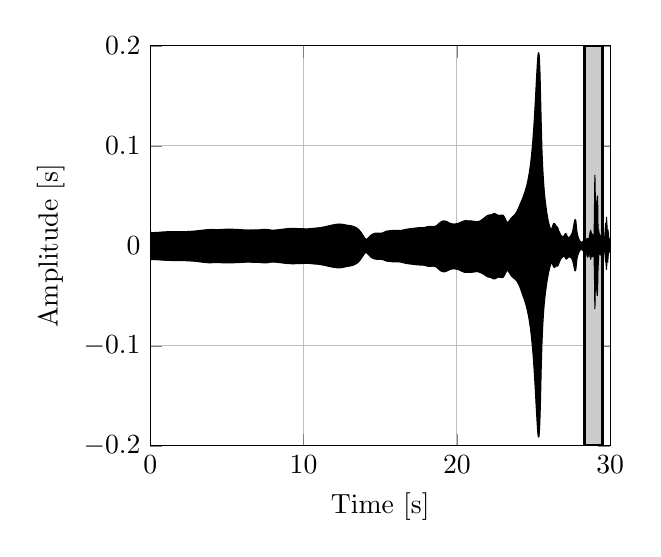
\begin{tikzpicture}

\begin{axis}[%
width=2.3in,
height=2in,
at={(1.011in,0.642in)},
scale only axis,
xmin=0,
xmax=30,
xmajorgrids,
ymin=-0.2,
ymax=0.2,
ymajorgrids,
xlabel={Time [s]},
ylabel={Amplitude [s]},
axis background/.style={fill=white}
]
\node[rectangle,draw, fill=black!20, minimum height=2in, minimum width=1pt, line width=1pt] at (axis cs:28.9,0) {};
\addplot[fill=black,draw=black,forget plot] plot table[row sep=crcr]{%
2.08333333333333e-05	0.0174441337585449\\
0.0250416666666667	0.013525128364563\\
0.0500625	0.013148307800293\\
0.0750833333333333	0.0131036043167114\\
0.100104166666667	0.0130690336227417\\
0.125125	0.0130878686904907\\
0.150145833333333	0.0131148099899292\\
0.175166666666667	0.0131456851959229\\
0.2001875	0.0131820440292358\\
0.225208333333333	0.0131937265396118\\
0.250229166666667	0.013242244720459\\
0.27525	0.0132321119308472\\
0.300270833333333	0.0132625102996826\\
0.325291666666667	0.0132992267608643\\
0.3503125	0.0133000612258911\\
0.375333333333333	0.0133060216903687\\
0.400354166666667	0.0133442878723145\\
0.425375	0.0133682489395142\\
0.450395833333333	0.0134040117263794\\
0.475416666666667	0.0134208202362061\\
0.5004375	0.0134366750717163\\
0.525458333333333	0.0134779214859009\\
0.550479166666667	0.013481616973877\\
0.5755	0.0135024785995483\\
0.600520833333333	0.0135313272476196\\
0.625541666666667	0.0135687589645386\\
0.6505625	0.0135985612869263\\
0.675583333333333	0.013633131980896\\
0.700604166666667	0.0136561393737793\\
0.725625	0.0136919021606445\\
0.750645833333333	0.0137306451797485\\
0.775666666666667	0.0137556791305542\\
0.8006875	0.01378333568573\\
0.825708333333333	0.0138041973114014\\
0.850729166666667	0.0138405561447144\\
0.87575	0.0138554573059082\\
0.900770833333333	0.0138554573059082\\
0.925791666666667	0.0138950347900391\\
0.9508125	0.0139113664627075\\
0.975833333333333	0.0139317512512207\\
1.00085416666667	0.0139557123184204\\
1.025875	0.0139747858047485\\
1.05089583333333	0.0140010118484497\\
1.07591666666667	0.0140320062637329\\
1.1009375	0.0140565633773804\\
1.12595833333333	0.0140770673751831\\
1.15097916666667	0.0140986442565918\\
1.176	0.0141662359237671\\
1.20102083333333	0.0141526460647583\\
1.22604166666667	0.0141149759292603\\
1.2510625	0.0141333341598511\\
1.27608333333333	0.0141546726226807\\
1.30110416666667	0.0141855478286743\\
1.326125	0.014235258102417\\
1.35114583333333	0.0142221450805664\\
1.37616666666667	0.0142310857772827\\
1.4011875	0.0142514705657959\\
1.42620833333333	0.0142489671707153\\
1.45122916666667	0.0142501592636108\\
1.47625	0.0142405033111572\\
1.50127083333333	0.0142426490783691\\
1.52629166666667	0.014230489730835\\
1.5513125	0.0142196416854858\\
1.57633333333333	0.0141897201538086\\
1.60135416666667	0.0141717195510864\\
1.626375	0.0141717195510864\\
1.65139583333333	0.0141562223434448\\
1.67641666666667	0.0141308307647705\\
1.7014375	0.0141433477401733\\
1.72645833333333	0.0141233205795288\\
1.75147916666667	0.0141158103942871\\
1.7765	0.0141146183013916\\
1.80152083333333	0.0140886306762695\\
1.82654166666667	0.0140882730484009\\
1.8515625	0.0140790939331055\\
1.87658333333333	0.0140920877456665\\
1.90160416666667	0.0140787363052368\\
1.926625	0.0140824317932129\\
1.95164583333333	0.014080286026001\\
1.97666666666667	0.0140800476074219\\
2.0016875	0.0140819549560547\\
2.02670833333333	0.0140724182128906\\
2.05172916666667	0.0140804052352905\\
2.07675	0.0140852928161621\\
2.10177083333333	0.0140907764434814\\
2.12679166666667	0.0141453742980957\\
2.1518125	0.0141433477401733\\
2.17683333333333	0.0141167640686035\\
2.20185416666667	0.014110803604126\\
2.226875	0.014117956161499\\
2.25189583333333	0.0141313076019287\\
2.27691666666667	0.01416015625\\
2.3019375	0.0141942501068115\\
2.32695833333333	0.0142010450363159\\
2.35197916666667	0.0142147541046143\\
2.377	0.0142277479171753\\
2.40202083333333	0.014255166053772\\
2.42704166666667	0.0142706632614136\\
2.4520625	0.0142948627471924\\
2.47708333333333	0.0143097639083862\\
2.50210416666667	0.014333963394165\\
2.527125	0.0143415927886963\\
2.55214583333333	0.0143803358078003\\
2.57716666666667	0.0144015550613403\\
2.6021875	0.0144282579421997\\
2.62720833333333	0.0144572257995605\\
2.65222916666667	0.0144776105880737\\
2.67725	0.0145164728164673\\
2.70227083333333	0.0145268440246582\\
2.72729166666667	0.0144838094711304\\
2.7523125	0.0145807266235352\\
2.77733333333333	0.0146057605743408\\
2.80235416666667	0.014631986618042\\
2.827375	0.0146661996841431\\
2.85239583333333	0.0147078037261963\\
2.87741666666667	0.0147354602813721\\
2.9024375	0.0147578716278076\\
2.92745833333333	0.0148038864135742\\
2.95247916666667	0.0148260593414307\\
2.9775	0.0148706436157227\\
3.00252083333333	0.0148930549621582\\
3.02754166666667	0.0149344205856323\\
3.0525625	0.0149737596511841\\
3.07758333333333	0.0150246620178223\\
3.10260416666667	0.0150657892227173\\
3.127625	0.0151075124740601\\
3.15264583333333	0.0151689052581787\\
3.17766666666667	0.0152368545532227\\
3.2026875	0.0152426958084106\\
3.22770833333333	0.0153077840805054\\
3.25272916666667	0.0153446197509766\\
3.27775	0.0153803825378418\\
3.30277083333333	0.0154129266738892\\
3.32779166666667	0.0154589414596558\\
3.3528125	0.0155411958694458\\
3.37783333333333	0.0155452489852905\\
3.40285416666667	0.0155919790267944\\
3.427875	0.0156158208847046\\
3.45289583333333	0.0156674385070801\\
3.47791666666667	0.0156955718994141\\
3.5029375	0.0157450437545776\\
3.52795833333333	0.0157967805862427\\
3.55297916666667	0.0158439874649048\\
3.578	0.0158843994140625\\
3.60302083333333	0.0159142017364502\\
3.62804166666667	0.0159745216369629\\
3.6530625	0.0160062313079834\\
3.67808333333333	0.0160480737686157\\
3.70310416666667	0.0160622596740723\\
3.728125	0.0160926580429077\\
3.75314583333333	0.0161361694335938\\
3.77816666666667	0.0161548852920532\\
3.8031875	0.0161689519882202\\
3.82820833333333	0.0162111520767212\\
3.85322916666667	0.0162196159362793\\
3.87825	0.0162382125854492\\
3.90327083333333	0.0162340402603149\\
3.92829166666667	0.0162550210952759\\
3.9533125	0.0162825584411621\\
3.97833333333333	0.016268253326416\\
4.00335416666667	0.0162605047225952\\
4.028375	0.0162662267684937\\
4.05339583333333	0.0162646770477295\\
4.07841666666667	0.0162562131881714\\
4.1034375	0.0162479877471924\\
4.12845833333333	0.0162286758422852\\
4.15347916666667	0.0162270069122314\\
4.1785	0.0162371397018433\\
4.20352083333333	0.0162290334701538\\
4.22854166666667	0.0162320137023926\\
4.2535625	0.0162011384963989\\
4.27858333333333	0.0161998271942139\\
4.30360416666667	0.0161756277084351\\
4.328625	0.0161881446838379\\
4.35364583333333	0.0161887407302856\\
4.37866666666667	0.0161789655685425\\
4.4036875	0.0161731243133545\\
4.42870833333333	0.0161886215209961\\
4.45372916666667	0.0162254571914673\\
4.47875	0.0162070989608765\\
4.50377083333333	0.0162215232849121\\
4.52879166666667	0.0162445306777954\\
4.5538125	0.0162478685379028\\
4.57883333333333	0.0162779092788696\\
4.60385416666667	0.0163146257400513\\
4.628875	0.0163321495056152\\
4.65389583333333	0.0163751840591431\\
4.67891666666667	0.0163940191268921\\
4.7039375	0.0164142847061157\\
4.72895833333333	0.0164343118667603\\
4.75397916666667	0.0164676904678345\\
4.779	0.0164873600006104\\
4.80402083333333	0.0164920091629028\\
4.82904166666667	0.0165045261383057\\
4.8540625	0.0165075063705444\\
4.87908333333333	0.0164927244186401\\
4.90410416666667	0.0165128707885742\\
4.929125	0.0165145397186279\\
4.95414583333333	0.0165392160415649\\
4.97916666666667	0.0165292024612427\\
5.0041875	0.0165307521820068\\
5.02920833333333	0.0165344476699829\\
5.05422916666667	0.0165383815765381\\
5.07925	0.0165324211120605\\
5.10427083333333	0.0165327787399292\\
5.12929166666667	0.0165436267852783\\
5.1543125	0.0165482759475708\\
5.17933333333333	0.0165408849716187\\
5.20435416666667	0.0165520906448364\\
5.229375	0.0165524482727051\\
5.25439583333333	0.0165770053863525\\
5.27941666666667	0.0165494680404663\\
5.3044375	0.0165427923202515\\
5.32945833333333	0.0165486335754395\\
5.35447916666667	0.016539454460144\\
5.3795	0.0165292024612427\\
5.40452083333333	0.0165024995803833\\
5.42954166666667	0.0165091753005981\\
5.4545625	0.0165070295333862\\
5.47958333333333	0.0164998769760132\\
5.50460416666667	0.0164941549301147\\
5.529625	0.0164831876754761\\
5.55464583333333	0.0164557695388794\\
5.57966666666667	0.0164422988891602\\
5.6046875	0.0164165496826172\\
5.62970833333333	0.0164107084274292\\
5.65472916666667	0.0163847208023071\\
5.67975	0.0163700580596924\\
5.70477083333333	0.0163614749908447\\
5.72979166666667	0.0163367986679077\\
5.7548125	0.0162984132766724\\
5.77983333333333	0.0162603855133057\\
5.80485416666667	0.0162379741668701\\
5.829875	0.0161999464035034\\
5.85489583333333	0.0161981582641602\\
5.87991666666667	0.0161627531051636\\
5.9049375	0.0161465406417847\\
5.92995833333333	0.016115665435791\\
5.95497916666667	0.0160897970199585\\
5.98	0.0160585641860962\\
6.00502083333333	0.0160255432128906\\
6.03004166666667	0.0159686803817749\\
6.0550625	0.0159963369369507\\
6.08008333333333	0.0159759521484375\\
6.10510416666667	0.0159282684326172\\
6.130125	0.015892505645752\\
6.15514583333333	0.0158891677856445\\
6.18016666666667	0.0158644914627075\\
6.2051875	0.0158466100692749\\
6.23020833333333	0.0158360004425049\\
6.25522916666667	0.0158376693725586\\
6.28025	0.0158051252365112\\
6.30527083333333	0.0157734155654907\\
6.33029166666667	0.0157642364501953\\
6.3553125	0.015750527381897\\
6.38033333333333	0.0157539844512939\\
6.40535416666667	0.0157500505447388\\
6.430375	0.0157680511474609\\
6.45539583333333	0.0157589912414551\\
6.48041666666667	0.0157626867294312\\
6.5054375	0.0157822370529175\\
6.53045833333333	0.0157740116119385\\
6.55547916666667	0.0157889127731323\\
6.5805	0.01578688621521\\
6.60552083333333	0.0157822370529175\\
6.63054166666667	0.015788197517395\\
6.6555625	0.0157915353775024\\
6.68058333333333	0.0158027410507202\\
6.70560416666667	0.0158090591430664\\
6.730625	0.0157994031906128\\
6.75564583333333	0.0158072710037231\\
6.78066666666667	0.0158181190490723\\
6.8056875	0.0157982110977173\\
6.83070833333333	0.0158140659332275\\
6.85572916666667	0.0158218145370483\\
6.88075	0.0158369541168213\\
6.90577083333333	0.015845775604248\\
6.93079166666667	0.0158636569976807\\
6.9558125	0.0158761739730835\\
6.98083333333333	0.0158882141113281\\
7.00585416666667	0.0158886909484863\\
7.030875	0.015921950340271\\
7.05589583333333	0.015964150428772\\
7.08091666666667	0.0159696340560913\\
7.1059375	0.0159767866134644\\
7.13095833333333	0.0160138607025146\\
7.15597916666667	0.0160485506057739\\
7.181	0.0161073207855225\\
7.20602083333333	0.0161236524581909\\
7.23104166666667	0.0161528587341309\\
7.2560625	0.0162006616592407\\
7.28108333333333	0.0162516832351685\\
7.30610416666667	0.0162925720214844\\
7.331125	0.0163209438323975\\
7.35614583333333	0.0163383483886719\\
7.38116666666667	0.0163733959197998\\
7.4061875	0.0163830518722534\\
7.43120833333333	0.0164109468460083\\
7.45622916666667	0.0164159536361694\\
7.48125	0.0164202451705933\\
7.50627083333333	0.01641845703125\\
7.53129166666667	0.0163898468017578\\
7.5563125	0.0163893699645996\\
7.58133333333333	0.0163614749908447\\
7.60635416666667	0.0163397789001465\\
7.631375	0.016291618347168\\
7.65639583333333	0.0162471532821655\\
7.68141666666667	0.0162198543548584\\
7.7064375	0.016148567199707\\
7.73145833333333	0.0160896778106689\\
7.75647916666667	0.016048789024353\\
7.7815	0.0159863233566284\\
7.80652083333333	0.0158941745758057\\
7.83154166666667	0.0158556699752808\\
7.8565625	0.0158106088638306\\
7.88158333333333	0.0157514810562134\\
7.90660416666667	0.0157146453857422\\
7.931625	0.0156705379486084\\
7.95664583333333	0.015657901763916\\
7.98166666666667	0.0156430006027222\\
8.0066875	0.015637993812561\\
8.03170833333333	0.0156441926956177\\
8.05672916666667	0.015630841255188\\
8.08175	0.0156583786010742\\
8.10677083333333	0.0156680345535278\\
8.13179166666667	0.0156958103179932\\
8.1568125	0.0157588720321655\\
8.18183333333333	0.0157665014266968\\
8.20685416666667	0.015811562538147\\
8.231875	0.0158299207687378\\
8.25689583333333	0.0158756971359253\\
8.28191666666667	0.0159240961074829\\
8.3069375	0.0159738063812256\\
8.33195833333333	0.0160108804702759\\
8.35697916666667	0.01605224609375\\
8.382	0.0161123275756836\\
8.40702083333333	0.0161582231521606\\
8.43204166666667	0.0161970853805542\\
8.4570625	0.0162638425827026\\
8.48208333333333	0.0163058042526245\\
8.50710416666667	0.0163264274597168\\
8.532125	0.0163748264312744\\
8.55714583333333	0.016425609588623\\
8.58216666666667	0.0164724588394165\\
8.6071875	0.0164806842803955\\
8.63220833333333	0.0165771245956421\\
8.65722916666667	0.0166155099868774\\
8.68225	0.0166538953781128\\
8.70727083333333	0.0166980028152466\\
8.73229166666667	0.0167548656463623\\
8.7573125	0.0168157815933228\\
8.78233333333333	0.0168620347976685\\
8.80735416666667	0.0168946981430054\\
8.832375	0.0169271230697632\\
8.85739583333333	0.0169821977615356\\
8.88241666666667	0.0170294046401978\\
8.9074375	0.0170701742172241\\
8.93245833333333	0.0171375274658203\\
8.95747916666667	0.0171374082565308\\
8.9825	0.0171587467193604\\
9.00752083333333	0.0172109603881836\\
9.03254166666667	0.017237663269043\\
9.0575625	0.0172935724258423\\
9.08258333333333	0.0173063278198242\\
9.10760416666667	0.0173218250274658\\
9.132625	0.0173497200012207\\
9.15764583333333	0.0173478126525879\\
9.18266666666667	0.0173822641372681\\
9.2076875	0.0173777341842651\\
9.23270833333333	0.0174020528793335\\
9.25772916666667	0.0174028873443604\\
9.28275	0.0174024105072021\\
9.30777083333333	0.0174020528793335\\
9.33279166666667	0.017372727394104\\
9.3578125	0.017397403717041\\
9.38283333333333	0.017382025718689\\
9.40785416666667	0.0173285007476807\\
9.432875	0.017330527305603\\
9.45789583333333	0.0173323154449463\\
9.48291666666667	0.0173298120498657\\
9.5079375	0.0173071622848511\\
9.53295833333333	0.0172946453094482\\
9.55797916666667	0.0172981023788452\\
9.583	0.0172525644302368\\
9.60802083333333	0.0172533988952637\\
9.63304166666667	0.0172268152236938\\
9.6580625	0.0172150135040283\\
9.68308333333333	0.0172126293182373\\
9.70810416666667	0.0172011852264404\\
9.733125	0.0171859264373779\\
9.75814583333333	0.0171804428100586\\
9.78316666666667	0.0171525478363037\\
9.8081875	0.0171377658843994\\
9.83320833333334	0.0171386003494263\\
9.85822916666667	0.0171124935150146\\
9.88325	0.0171166658401489\\
9.90827083333333	0.0170993804931641\\
9.93329166666667	0.0170944929122925\\
9.9583125	0.0170706510543823\\
9.98333333333333	0.0170501470565796\\
10.0083541666667	0.0170356035232544\\
10.033375	0.0169914960861206\\
10.0583958333333	0.0170005559921265\\
10.0834166666667	0.0170102119445801\\
10.1084375	0.0169705152511597\\
10.1334583333333	0.0169491767883301\\
10.1584791666667	0.0169483423233032\\
10.1835	0.0169246196746826\\
10.2085208333333	0.0169349908828735\\
10.2335416666667	0.016913890838623\\
10.2585625	0.016938328742981\\
10.2835833333333	0.0169572830200195\\
10.3086041666667	0.0169775485992432\\
10.333625	0.016999363899231\\
10.3586458333333	0.0170327425003052\\
10.3836666666667	0.0170744657516479\\
10.4086875	0.0170915126800537\\
10.4337083333333	0.0171260833740234\\
10.4587291666667	0.0171712636947632\\
10.48375	0.0172317028045654\\
10.5087708333333	0.0172442197799683\\
10.5337916666667	0.0172771215438843\\
10.5588125	0.017345666885376\\
10.5838333333333	0.0173889398574829\\
10.6088541666667	0.0174278020858765\\
10.633875	0.0174736976623535\\
10.6588958333333	0.0175179243087769\\
10.6839166666667	0.017504096031189\\
10.7089375	0.0175975561141968\\
10.7339583333333	0.0176342725753784\\
10.7589791666667	0.0176651477813721\\
10.784	0.0177170038223267\\
10.8090208333333	0.0177382230758667\\
10.8340416666667	0.0177578926086426\\
10.8590625	0.0177834033966064\\
10.8840833333333	0.0178287029266357\\
10.9091041666667	0.0178596973419189\\
10.934125	0.0178934335708618\\
10.9591458333333	0.0179351568222046\\
10.9841666666667	0.0179930925369263\\
11.0091875	0.0180190801620483\\
11.0342083333333	0.0180590152740479\\
11.0592291666667	0.0180873870849609\\
11.08425	0.0181617736816406\\
11.1092708333333	0.0181983709335327\\
11.1342916666667	0.0182547569274902\\
11.1593125	0.018323540687561\\
11.1843333333333	0.018383264541626\\
11.2093541666667	0.0184645652770996\\
11.234375	0.0185511112213135\\
11.2593958333333	0.0186281204223633\\
11.2844166666667	0.0186648368835449\\
11.3094375	0.0187809467315674\\
11.3344583333333	0.0188539028167725\\
11.3594791666667	0.0189625024795532\\
11.3845	0.0190408229827881\\
11.4095208333333	0.0191167593002319\\
11.4345416666667	0.0191928148269653\\
11.4595625	0.019289493560791\\
11.4845833333333	0.0194246768951416\\
11.5096041666667	0.0194790363311768\\
11.534625	0.0195668935775757\\
11.5596458333333	0.0196346044540405\\
11.5846666666667	0.0197362899780273\\
11.6096875	0.0198198556900024\\
11.6347083333333	0.0198944807052612\\
11.6597291666667	0.0199992656707764\\
11.68475	0.0200852155685425\\
11.7097708333333	0.0201708078384399\\
11.7347916666667	0.0202442407608032\\
11.7598125	0.0203417539596558\\
11.7848333333333	0.020447850227356\\
11.8098541666667	0.0205179452896118\\
11.834875	0.020601749420166\\
11.8598958333333	0.0206559896469116\\
11.8849166666667	0.0207802057266235\\
11.9099375	0.0208553075790405\\
11.9349583333333	0.0209276676177979\\
11.9599791666667	0.0209884643554688\\
11.985	0.0210902690887451\\
12.0100208333333	0.0211566686630249\\
12.0350416666667	0.0212430953979492\\
12.0600625	0.0213093757629395\\
12.0850833333333	0.0213801860809326\\
12.1101041666667	0.0214052200317383\\
12.135125	0.0214844942092896\\
12.1601458333333	0.0215476751327515\\
12.1851666666667	0.0216346979141235\\
12.2101875	0.0216710567474365\\
12.2352083333333	0.0217214822769165\\
12.2602291666667	0.0217512845993042\\
12.28525	0.0217370986938477\\
12.3102708333333	0.0217386484146118\\
12.3352916666667	0.0217440128326416\\
12.3603125	0.0217629671096802\\
12.3853333333333	0.0217190980911255\\
12.4103541666667	0.0217164754867554\\
12.435375	0.0216363668441772\\
12.4603958333333	0.0216211080551147\\
12.4854166666667	0.021581768989563\\
12.5104375	0.0215216875076294\\
12.5354583333333	0.021467924118042\\
12.5604791666667	0.0213643312454224\\
12.5855	0.021304726600647\\
12.6105208333333	0.0212384462356567\\
12.6355416666667	0.0211762189865112\\
12.6605625	0.0210961103439331\\
12.6855833333333	0.0210355520248413\\
12.7106041666667	0.0209527015686035\\
12.735625	0.0208666324615479\\
12.7606458333333	0.0208185911178589\\
12.7856666666667	0.0207582712173462\\
12.8106875	0.0206890106201172\\
12.8357083333333	0.0206308364868164\\
12.8607291666667	0.0205554962158203\\
12.88575	0.0205261707305908\\
12.9107708333333	0.0204222202301025\\
12.9357916666667	0.0204188823699951\\
12.9608125	0.0203204154968262\\
12.9858333333333	0.0202691555023193\\
13.0108541666667	0.0202019214630127\\
13.035875	0.0201456546783447\\
13.0608958333333	0.0200655460357666\\
13.0859166666667	0.0200191736221313\\
13.1109375	0.0199253559112549\\
13.1359583333333	0.0198445320129395\\
13.1609791666667	0.0197505950927734\\
13.186	0.0197038650512695\\
13.2110208333333	0.0195786952972412\\
13.2360416666667	0.019476056098938\\
13.2610625	0.0193073749542236\\
13.2860833333333	0.0191764831542969\\
13.3111041666667	0.0190207958221436\\
13.336125	0.0188961029052734\\
13.3611458333333	0.0186749696731567\\
13.3861666666667	0.0185122489929199\\
13.4111875	0.0183169841766357\\
13.4362083333333	0.0180661678314209\\
13.4612291666667	0.017853856086731\\
13.48625	0.0175918340682983\\
13.5112708333333	0.0173110961914062\\
13.5362916666667	0.0169925689697266\\
13.5613125	0.0166597366333008\\
13.5863333333333	0.0163099765777588\\
13.6113541666667	0.0159174203872681\\
13.636375	0.0155293941497803\\
13.6613958333333	0.0150763988494873\\
13.6864166666667	0.0146143436431885\\
13.7114375	0.014168381690979\\
13.7364583333333	0.0136096477508545\\
13.7614791666667	0.0130655765533447\\
13.7865	0.0125436782836914\\
13.8115208333333	0.0119357109069824\\
13.8365416666667	0.0113338232040405\\
13.8615625	0.0106756687164307\\
13.8865833333333	0.0100915431976318\\
13.9116041666667	0.00947129726409912\\
13.936625	0.00886750221252441\\
13.9616458333333	0.00825822353363037\\
13.9866666666667	0.00778257846832275\\
14.0116875	0.00735759735107422\\
14.0367083333333	0.00696361064910889\\
14.0617291666667	0.00667524337768555\\
14.08675	0.00652050971984863\\
14.1117708333333	0.00652647018432617\\
14.1367916666667	0.00670945644378662\\
14.1618125	0.00699913501739502\\
14.1868333333333	0.00733792781829834\\
14.2118541666667	0.0077139139175415\\
14.236875	0.00815272331237793\\
14.2618958333333	0.00860869884490967\\
14.2869166666667	0.00900518894195557\\
14.3119375	0.00939702987670898\\
14.3369583333333	0.00978922843933105\\
14.3619791666667	0.0101321935653687\\
14.387	0.0104804039001465\\
14.4120208333333	0.0107772350311279\\
14.4370416666667	0.0110471248626709\\
14.4620625	0.0112928152084351\\
14.4870833333333	0.0115351676940918\\
14.5121041666667	0.0117450952529907\\
14.537125	0.0118981599807739\\
14.5621458333333	0.0120600461959839\\
14.5871666666667	0.0121918916702271\\
14.6121875	0.0123043060302734\\
14.6372083333333	0.0123888254165649\\
14.6622291666667	0.0124760866165161\\
14.68725	0.0125365257263184\\
14.7122708333333	0.0126163959503174\\
14.7372916666667	0.0126279592514038\\
14.7623125	0.0126475095748901\\
14.7873333333333	0.0126579999923706\\
14.8123541666667	0.0126771926879883\\
14.837375	0.0126643180847168\\
14.8623958333333	0.0126522779464722\\
14.8874166666667	0.0126442909240723\\
14.9124375	0.0126438140869141\\
14.9374583333333	0.0126296281814575\\
14.9624791666667	0.0126005411148071\\
14.9875	0.0125808715820312\\
15.0125208333333	0.0125870704650879\\
15.0375416666667	0.0125871896743774\\
15.0625625	0.0126022100448608\\
15.0875833333333	0.0126547813415527\\
15.1126041666667	0.0127360820770264\\
15.137625	0.0128141641616821\\
15.1626458333333	0.0129730701446533\\
15.1876666666667	0.0131022930145264\\
15.2126875	0.0132739543914795\\
15.2377083333333	0.0134528875350952\\
15.2627291666667	0.0136306285858154\\
15.28775	0.0138425827026367\\
15.3127708333333	0.0140299797058105\\
15.3377916666667	0.014187216758728\\
15.3628125	0.0143324136734009\\
15.3878333333333	0.0144814252853394\\
15.4128541666667	0.0145851373672485\\
15.437875	0.0147069692611694\\
15.4628958333333	0.0147304534912109\\
15.4879166666667	0.014826774597168\\
15.5129375	0.0148801803588867\\
15.5379583333333	0.0149414539337158\\
15.5629791666667	0.0149836540222168\\
15.588	0.0150250196456909\\
15.6130208333333	0.0150867700576782\\
15.6380416666667	0.0151267051696777\\
15.6630625	0.0151498317718506\\
15.6880833333333	0.0151907205581665\\
15.7131041666667	0.0152368545532227\\
15.738125	0.0152875185012817\\
15.7631458333333	0.0153127908706665\\
15.7881666666667	0.015317440032959\\
15.8131875	0.0153570175170898\\
15.8382083333333	0.0153809785842896\\
15.8632291666667	0.0153845548629761\\
15.88825	0.0154021978378296\\
15.9132708333333	0.0154201984405518\\
15.9382916666667	0.0154287815093994\\
15.9633125	0.0154200792312622\\
15.9883333333333	0.0154142379760742\\
16.0133541666667	0.0154227018356323\\
16.038375	0.0153951644897461\\
16.0633958333333	0.0153549909591675\\
16.0884166666667	0.0153504610061646\\
16.1134375	0.015299916267395\\
16.1384583333333	0.0152820348739624\\
16.1634791666667	0.0152640342712402\\
16.1885	0.0152740478515625\\
16.2135208333333	0.0152524709701538\\
16.2385416666667	0.0152736902236938\\
16.2635625	0.0152624845504761\\
16.2885833333333	0.0152912139892578\\
16.3136041666667	0.0153496265411377\\
16.338625	0.015373706817627\\
16.3636458333333	0.0154263973236084\\
16.3886666666667	0.0154972076416016\\
16.4136875	0.0155841112136841\\
16.4387083333333	0.0156378746032715\\
16.4637291666667	0.01569664478302\\
16.48875	0.015790581703186\\
16.5137708333333	0.0158723592758179\\
16.5387916666667	0.0159751176834106\\
16.5638125	0.0160551071166992\\
16.5888333333333	0.0161577463150024\\
16.6138541666667	0.0162507295608521\\
16.638875	0.0163224935531616\\
16.6638958333333	0.0163685083389282\\
16.6889166666667	0.0164364576339722\\
16.7139375	0.0165036916732788\\
16.7389583333333	0.0165603160858154\\
16.7639791666667	0.0166410207748413\\
16.789	0.0167248249053955\\
16.8140208333333	0.0167744159698486\\
16.8390416666667	0.016828179359436\\
16.8640625	0.0168788433074951\\
16.8890833333333	0.0169576406478882\\
16.9141041666667	0.016994833946228\\
16.939125	0.0170410871505737\\
16.9641458333333	0.0170806646347046\\
16.9891666666667	0.017139196395874\\
17.0141875	0.0172109603881836\\
17.0392083333333	0.0172618627548218\\
17.0642291666667	0.0173348188400269\\
17.08925	0.0173755884170532\\
17.1142708333333	0.0174448490142822\\
17.1392916666667	0.0174486637115479\\
17.1643125	0.0174803733825684\\
17.1893333333333	0.017526388168335\\
17.2143541666667	0.0175930261611938\\
17.239375	0.0176322460174561\\
17.2643958333333	0.0176610946655273\\
17.2894166666667	0.0177028179168701\\
17.3144375	0.0177712440490723\\
17.3394583333333	0.017817497253418\\
17.3644791666667	0.0178496837615967\\
17.3895	0.0178635120391846\\
17.4145208333333	0.0179288387298584\\
17.4395416666667	0.017961859703064\\
17.4645625	0.017999529838562\\
17.4895833333333	0.018022894859314\\
17.5146041666667	0.018062949180603\\
17.539625	0.0180728435516357\\
17.5646458333333	0.01810622215271\\
17.5896666666667	0.0180763006210327\\
17.6146875	0.0180631875991821\\
17.6397083333333	0.0180815458297729\\
17.6647291666667	0.0180732011795044\\
17.68975	0.0180611610412598\\
17.7147708333333	0.0180732011795044\\
17.7397916666667	0.0180991888046265\\
17.7648125	0.018126368522644\\
17.7898333333333	0.0181397199630737\\
17.8148541666667	0.0181893110275269\\
17.839875	0.0182832479476929\\
17.8648958333333	0.0183231830596924\\
17.8899166666667	0.0183992385864258\\
17.9149375	0.0184700489044189\\
17.9399583333333	0.0185521841049194\\
17.9649791666667	0.0186257362365723\\
17.99	0.0187492370605469\\
18.0150208333333	0.0188664197921753\\
18.0400416666667	0.0189815759658813\\
18.0650625	0.0190328359603882\\
18.0900833333333	0.0191329717636108\\
18.1151041666667	0.0192264318466187\\
18.140125	0.0192656517028809\\
18.1651458333333	0.0192974805831909\\
18.1901666666667	0.0193121433258057\\
18.2151875	0.0193363428115845\\
18.2402083333333	0.0193533897399902\\
18.2652291666667	0.0193248987197876\\
18.29025	0.0193346738815308\\
18.3152708333333	0.0193099975585938\\
18.3402916666667	0.0192739963531494\\
18.3653125	0.0192720890045166\\
18.3903333333333	0.0192562341690063\\
18.4153541666667	0.0192611217498779\\
18.440375	0.0192636251449585\\
18.4653958333333	0.0192465782165527\\
18.4904166666667	0.0192739963531494\\
18.5154375	0.0192666053771973\\
18.5404583333333	0.0192996263504028\\
18.5654791666667	0.0193842649459839\\
18.5905	0.0194982290267944\\
18.6155208333333	0.0196996927261353\\
18.6405416666667	0.0198712348937988\\
18.6655625	0.0201015472412109\\
18.6905833333333	0.02039635181427\\
18.7156041666667	0.0207115411758423\\
18.740625	0.02104651927948\\
18.7656458333333	0.0213632583618164\\
18.7906666666667	0.0217374563217163\\
18.8156875	0.0221004486083984\\
18.8407083333333	0.0224542617797852\\
18.8657291666667	0.0227910280227661\\
18.89075	0.023115873336792\\
18.9157708333333	0.0234055519104004\\
18.9407916666667	0.0236350297927856\\
18.9658125	0.0238840579986572\\
18.9908333333333	0.0240856409072876\\
19.0158541666667	0.0243097543716431\\
19.040875	0.0244883298873901\\
19.0658958333333	0.0246367454528809\\
19.0909166666667	0.0247553586959839\\
19.1159375	0.0248157978057861\\
19.1409583333333	0.0248211622238159\\
19.1659791666667	0.0248291492462158\\
19.191	0.0247656106948853\\
19.2160208333333	0.0247126817703247\\
19.2410416666667	0.0246188640594482\\
19.2660625	0.0245308876037598\\
19.2910833333333	0.024416446685791\\
19.3161041666667	0.0243091583251953\\
19.341125	0.0241603851318359\\
19.3661458333333	0.0239905118942261\\
19.3911666666667	0.0237839221954346\\
19.4161875	0.0236095190048218\\
19.4412083333333	0.0234092473983765\\
19.4662291666667	0.0231764316558838\\
19.49125	0.0229754447937012\\
19.5162708333333	0.022815465927124\\
19.5412916666667	0.0226483345031738\\
19.5663125	0.0224692821502686\\
19.5913333333333	0.0223290920257568\\
19.6163541666667	0.0222113132476807\\
19.641375	0.0221070051193237\\
19.6663958333333	0.0220341682434082\\
19.6914166666667	0.0219175815582275\\
19.7164375	0.0218663215637207\\
19.7414583333333	0.0218421220779419\\
19.7664791666667	0.0217581987380981\\
19.7915	0.021744966506958\\
19.8165208333333	0.0217596292495728\\
19.8415416666667	0.0217770338058472\\
19.8665625	0.0217828750610352\\
19.8915833333333	0.0218362808227539\\
19.9166041666667	0.0218791961669922\\
19.941625	0.0219467878341675\\
19.9666458333333	0.0220240354537964\\
19.9916666666667	0.0220874547958374\\
20.0166875	0.0221959352493286\\
20.0417083333333	0.022313117980957\\
20.0667291666667	0.0224117040634155\\
20.09175	0.0225427150726318\\
20.1167708333333	0.0226690769195557\\
20.1417916666667	0.0228263139724731\\
20.1668125	0.0229573249816895\\
20.1918333333333	0.0231013298034668\\
20.2168541666667	0.0232757329940796\\
20.241875	0.0234352350234985\\
20.2668958333333	0.0236291885375977\\
20.2919166666667	0.0237768888473511\\
20.3169375	0.023958683013916\\
20.3419583333333	0.0241364240646362\\
20.3669791666667	0.0242964029312134\\
20.392	0.0244518518447876\\
20.4170208333333	0.0246180295944214\\
20.4420416666667	0.0247514247894287\\
20.4670625	0.0248813629150391\\
20.4920833333333	0.0249801874160767\\
20.5171041666667	0.0250335931777954\\
20.542125	0.0250766277313232\\
20.5671458333333	0.0250948667526245\\
20.5921666666667	0.0251015424728394\\
20.6171875	0.0250868797302246\\
20.6422083333333	0.025084376335144\\
20.6672291666667	0.0250357389450073\\
20.69225	0.0249865055084229\\
20.7172708333333	0.0249638557434082\\
20.7422916666667	0.0249263048171997\\
20.7673125	0.0249083042144775\\
20.7923333333333	0.0248900651931763\\
20.8173541666667	0.0248545408248901\\
20.842375	0.0248538255691528\\
20.8673958333333	0.0248371362686157\\
20.8924166666667	0.0248321294784546\\
20.9174375	0.0248321294784546\\
20.9424583333333	0.0248123407363892\\
20.9674791666667	0.0248016119003296\\
20.9925	0.0247378349304199\\
21.0175208333333	0.0246872901916504\\
21.0425416666667	0.0246568918228149\\
21.0675625	0.0245620012283325\\
21.0925833333333	0.0245187282562256\\
21.1176041666667	0.0244406461715698\\
21.142625	0.0243560075759888\\
21.1676458333333	0.0242875814437866\\
21.1926666666667	0.0241986513137817\\
21.2176875	0.0241419076919556\\
21.2427083333333	0.0241051912307739\\
21.2677291666667	0.0240743160247803\\
21.29275	0.0240596532821655\\
21.3177708333333	0.0240672826766968\\
21.3427916666667	0.0241365432739258\\
21.3678125	0.0242211818695068\\
21.3928333333333	0.0242770910263062\\
21.4178541666667	0.0243664979934692\\
21.442875	0.0245187282562256\\
21.4678958333333	0.0246692895889282\\
21.4929166666667	0.0248323678970337\\
21.5179375	0.0250157117843628\\
21.5429583333333	0.0251970291137695\\
21.5679791666667	0.0254095792770386\\
21.593	0.0256576538085938\\
21.6180208333333	0.0259164571762085\\
21.6430416666667	0.0261667966842651\\
21.6680625	0.0264409780502319\\
21.6930833333333	0.0267170667648315\\
21.7181041666667	0.0269858837127686\\
21.743125	0.0273033380508423\\
21.7681458333333	0.0276157855987549\\
21.7931666666667	0.0278679132461548\\
21.8181875	0.0282278060913086\\
21.8432083333333	0.0285413265228271\\
21.8682291666667	0.0288461446762085\\
21.89325	0.029139518737793\\
21.9182708333333	0.0294617414474487\\
21.9432916666667	0.0297086238861084\\
21.9683125	0.0300043821334839\\
21.9933333333333	0.0302213430404663\\
22.0183541666667	0.0304399728775024\\
22.043375	0.0305919647216797\\
22.0683958333333	0.0306967496871948\\
22.0934166666667	0.0307843685150146\\
22.1184375	0.0307987928390503\\
22.1434583333333	0.030825138092041\\
22.1684791666667	0.0308159589767456\\
22.1935	0.0308229923248291\\
22.2185208333333	0.0309444665908813\\
22.2435416666667	0.0311071872711182\\
22.2685625	0.0312448740005493\\
22.2935833333333	0.0314546823501587\\
22.3186041666667	0.0316667556762695\\
22.343625	0.0318219661712646\\
22.3686458333333	0.0320000648498535\\
22.3936666666667	0.0320919752120972\\
22.4186875	0.0321664810180664\\
22.4437083333333	0.0321915149688721\\
22.4687291666667	0.0321606397628784\\
22.49375	0.0321078300476074\\
22.5187708333333	0.031922459602356\\
22.5437916666667	0.0317248106002808\\
22.5688125	0.031496524810791\\
22.5938333333333	0.0312548875808716\\
22.6188541666667	0.0311131477355957\\
22.643875	0.0308171510696411\\
22.6688958333333	0.030713677406311\\
22.6939166666667	0.030561089515686\\
22.7189375	0.0304679870605469\\
22.7439583333333	0.0304421186447144\\
22.7689791666667	0.0303603410720825\\
22.794	0.0303953886032104\\
22.8190208333333	0.0304563045501709\\
22.8440416666667	0.0305156707763672\\
22.8690625	0.0305367708206177\\
22.8940833333333	0.0306057929992676\\
22.9191041666667	0.0306382179260254\\
22.944125	0.0306912660598755\\
22.9691458333333	0.0306316614151001\\
22.9941666666667	0.0306066274642944\\
23.0191875	0.0304591655731201\\
23.0442083333333	0.0300365686416626\\
23.0692291666667	0.0294849872589111\\
23.09425	0.0287594795227051\\
23.1192708333333	0.0279767513275146\\
23.1442916666667	0.027154803276062\\
23.1693125	0.0264017581939697\\
23.1943333333333	0.0256999731063843\\
23.2193541666667	0.0246617794036865\\
23.244375	0.0238051414489746\\
23.2693958333333	0.0236220359802246\\
23.2944166666667	0.0233170986175537\\
23.3194375	0.0234898328781128\\
23.3444583333333	0.0237802267074585\\
23.3694791666667	0.0241098403930664\\
23.3945	0.024639368057251\\
23.4195208333333	0.0251232385635376\\
23.4445416666667	0.0256147384643555\\
23.4695625	0.0261942148208618\\
23.4945833333333	0.0267441272735596\\
23.5196041666667	0.0272728204727173\\
23.544625	0.0277079343795776\\
23.5696458333333	0.0281523466110229\\
23.5946666666667	0.0285365581512451\\
23.6196875	0.0288980007171631\\
23.6447083333333	0.0291863679885864\\
23.6697291666667	0.0294959545135498\\
23.69475	0.029880166053772\\
23.7197708333333	0.0302121639251709\\
23.7447916666667	0.0305644273757935\\
23.7698125	0.0310232639312744\\
23.7948333333333	0.0315340757369995\\
23.8198541666667	0.0320580005645752\\
23.844875	0.0326471328735352\\
23.8698958333333	0.0332018136978149\\
23.8949166666667	0.0337858200073242\\
23.9199375	0.0345264673233032\\
23.9449583333333	0.0352761745452881\\
23.9699791666667	0.0361440181732178\\
23.995	0.0370364189147949\\
24.0200208333333	0.0377423763275146\\
24.0450416666667	0.0387363433837891\\
24.0700625	0.0396305322647095\\
24.0950833333333	0.0405175685882568\\
24.1201041666667	0.041479229927063\\
24.145125	0.0423545837402344\\
24.1701458333333	0.0432147979736328\\
24.1951666666667	0.044137716293335\\
24.2201875	0.0450013875961304\\
24.2452083333333	0.0459293127059937\\
24.2702291666667	0.0469129085540771\\
24.29525	0.0479274988174438\\
24.3202708333333	0.0489280223846436\\
24.3452916666667	0.0500307083129883\\
24.3703125	0.0510417222976685\\
24.3953333333333	0.052181601524353\\
24.4203541666667	0.0532969236373901\\
24.445375	0.0544567108154297\\
24.4703958333333	0.0556988716125488\\
24.4954166666667	0.056898832321167\\
24.5204375	0.0582900047302246\\
24.5454583333333	0.0596746206283569\\
24.5704791666667	0.0611917972564697\\
24.5955	0.0627651214599609\\
24.6205208333333	0.0645843744277954\\
24.6455416666667	0.0664654970169067\\
24.6705625	0.0684857368469238\\
24.6955833333333	0.0705987215042114\\
24.7206041666667	0.0729748010635376\\
24.745625	0.0752949714660645\\
24.7706458333333	0.0780850648880005\\
24.7956666666667	0.0809968709945679\\
24.8206875	0.084004282951355\\
24.8457083333333	0.0875474214553833\\
24.8707291666667	0.0909876823425293\\
24.89575	0.0951199531555176\\
24.9207708333333	0.0991923809051514\\
24.9457916666667	0.103655219078064\\
24.9708125	0.108772873878479\\
24.9958333333333	0.114107251167297\\
25.0208541666667	0.119699358940125\\
25.045875	0.125730037689209\\
25.0708958333333	0.132137656211853\\
25.0959166666667	0.139050245285034\\
25.1209375	0.146229147911072\\
25.1459583333333	0.153596758842468\\
25.1709791666667	0.161020040512085\\
25.196	0.168261528015137\\
25.2210208333333	0.175299406051636\\
25.2460416666667	0.181927919387817\\
25.2710625	0.187173366546631\\
25.2960833333333	0.191585659980774\\
25.3211041666667	0.192880272865295\\
25.346125	0.192724227905273\\
25.3711458333333	0.189618349075317\\
25.3961666666667	0.181955933570862\\
25.4211875	0.171445846557617\\
25.4462083333333	0.155550122261047\\
25.4712291666667	0.139785528182983\\
25.49625	0.123754620552063\\
25.5212708333333	0.109553933143616\\
25.5462916666667	0.0963232517242432\\
25.5713125	0.086665153503418\\
25.5963333333333	0.0784014463424683\\
25.6213541666667	0.071405291557312\\
25.646375	0.0651895999908447\\
25.6713958333333	0.0598506927490234\\
25.6964166666667	0.0547468662261963\\
25.7214375	0.050620436668396\\
25.7464583333333	0.0471398830413818\\
25.7714791666667	0.043710470199585\\
25.7965	0.0407135486602783\\
25.8215208333333	0.0378057956695557\\
25.8465416666667	0.0348886251449585\\
25.8715625	0.0322417020797729\\
25.8965833333333	0.0300600528717041\\
25.9216041666667	0.0277225971221924\\
25.946625	0.025759220123291\\
25.9716458333333	0.0239880084991455\\
25.9966666666667	0.0221370458602905\\
26.0216875	0.0206685066223145\\
26.0467083333333	0.0193742513656616\\
26.0717291666667	0.0183048248291016\\
26.09675	0.0174481868743896\\
26.1217708333333	0.0168154239654541\\
26.1467916666667	0.0165709257125854\\
26.1718125	0.0168967247009277\\
26.1968333333333	0.0176175832748413\\
26.2218541666667	0.0186170339584351\\
26.246875	0.0197421312332153\\
26.2718958333333	0.0208824872970581\\
26.2969166666667	0.0218906402587891\\
26.3219375	0.0222227573394775\\
26.3469583333333	0.0223579406738281\\
26.3719791666667	0.0221942663192749\\
26.397	0.0217078924179077\\
26.4220208333333	0.0209922790527344\\
26.4470416666667	0.0202728509902954\\
26.4720625	0.0196545124053955\\
26.4970833333333	0.0193988084793091\\
26.5221041666667	0.0191034078598022\\
26.547125	0.0187299251556396\\
26.5721458333333	0.0180537700653076\\
26.5971666666667	0.0168862342834473\\
26.6221875	0.015802264213562\\
26.6472083333333	0.0147438049316406\\
26.6722291666667	0.0138993263244629\\
26.69725	0.0131711959838867\\
26.7222708333333	0.0123679637908936\\
26.7472916666667	0.0115710496902466\\
26.7723125	0.0107738971710205\\
26.7973333333333	0.0101497173309326\\
26.8223541666667	0.00979006290435791\\
26.847375	0.00962471961975098\\
26.8723958333333	0.00949633121490479\\
26.8974166666667	0.00931215286254883\\
26.9224375	0.00916421413421631\\
26.9474583333333	0.00920677185058594\\
26.9724791666667	0.00953972339630127\\
26.9975	0.0102084875106812\\
27.0225208333333	0.0108667612075806\\
27.0475416666667	0.0115419626235962\\
27.0725625	0.0120722055435181\\
27.0975833333333	0.0121549367904663\\
27.1226041666667	0.0118545293807983\\
27.147625	0.0111083984375\\
27.1726458333333	0.0101121664047241\\
27.1976666666667	0.0093076229095459\\
27.2226875	0.00873386859893799\\
27.2477083333333	0.00842678546905518\\
27.2727291666667	0.00834882259368896\\
27.29775	0.00836217403411865\\
27.3227708333333	0.00848746299743652\\
27.3477916666667	0.00875973701477051\\
27.3728125	0.0090184211730957\\
27.3978333333333	0.00947034358978271\\
27.4228541666667	0.00991213321685791\\
27.447875	0.0106494426727295\\
27.4728958333333	0.0113028287887573\\
27.4979166666667	0.012182354927063\\
27.5229375	0.0131195783615112\\
27.5479583333333	0.0144155025482178\\
27.5729791666667	0.0162382125854492\\
27.598	0.0181559324264526\\
27.6230208333333	0.0203871726989746\\
27.6480416666667	0.0227947235107422\\
27.6730625	0.0248361825942993\\
27.6980833333333	0.0259034633636475\\
27.7231041666667	0.0261249542236328\\
27.748125	0.0256080627441406\\
27.7731458333333	0.0226942300796509\\
27.7981666666667	0.0178313255310059\\
27.8231875	0.0147879123687744\\
27.8482083333333	0.0123029947280884\\
27.8732291666667	0.0105404853820801\\
27.89825	0.00934135913848877\\
27.9232708333333	0.00792503356933594\\
27.9482916666667	0.00695645809173584\\
27.9733125	0.00611364841461182\\
27.9983333333333	0.00526881217956543\\
28.0233541666667	0.00476109981536865\\
28.048375	0.00428164005279541\\
28.0733958333333	0.00390028953552246\\
28.0984166666667	0.00352144241333008\\
28.1234375	0.00320971012115479\\
28.1484583333333	0.00320219993591309\\
28.1734791666667	0.00377941131591797\\
28.1985	0.0043492317199707\\
28.2235208333333	0.00466501712799072\\
28.2485416666667	0.00484251976013184\\
28.2735625	0.00487172603607178\\
28.2985833333333	0.00505399703979492\\
28.3236041666667	0.00524246692657471\\
28.348625	0.00562095642089844\\
28.3736458333333	0.00589895248413086\\
28.3986666666667	0.00605738162994385\\
28.4236875	0.00629270076751709\\
28.4487083333333	0.00658106803894043\\
28.4737291666667	0.00671696662902832\\
28.49875	0.00694727897644043\\
28.5237708333333	0.0074467658996582\\
28.5487916666667	0.00746893882751465\\
28.5738125	0.00671839714050293\\
28.5988333333333	0.00586915016174316\\
28.6238541666667	0.00598013401031494\\
28.648875	0.00930511951446533\\
28.6738958333333	0.0123151540756226\\
28.6989166666667	0.0111576318740845\\
28.7239375	0.0158895254135132\\
28.7489583333333	0.00994598865509033\\
28.7739791666667	0.0123809576034546\\
28.799	0.0107604265213013\\
28.8240208333333	0.00990724563598633\\
28.8490416666667	0.00613832473754883\\
28.8740625	0.0101600885391235\\
28.8990833333333	0.00902903079986572\\
28.9241041666667	0.00855207443237305\\
28.949125	0.00797700881958008\\
28.9741458333333	0.0380454063415527\\
28.9991666666667	0.0708549022674561\\
29.0241875	0.0490773916244507\\
29.0492083333333	0.0407736301422119\\
29.0742291666667	0.0349804162979126\\
29.09925	0.0337502956390381\\
29.1242708333333	0.0392665863037109\\
29.1492916666667	0.0477851629257202\\
29.1743125	0.0501984357833862\\
29.1993333333333	0.0208961963653564\\
29.2243541666667	0.0139025449752808\\
29.249375	0.0146907567977905\\
29.2743958333333	0.0124069452285767\\
29.2994166666667	0.0113190412521362\\
29.3244375	0.0109615325927734\\
29.3494583333333	0.00985002517700195\\
29.3744791666667	0.0061262845993042\\
29.3995	0.00371837615966797\\
29.4245208333333	0.00360357761383057\\
29.4495416666667	0.00346684455871582\\
29.4745625	0.0025477409362793\\
29.4995833333333	0.0020289421081543\\
29.5246041666667	0.0020139217376709\\
29.549625	0.00211250782012939\\
29.5746458333333	0.00222396850585938\\
29.5996666666667	0.00345098972320557\\
29.6246875	0.0047835111618042\\
29.6497083333333	0.0106549263000488\\
29.6747291666667	0.0167301893234253\\
29.69975	0.0227276086807251\\
29.7247708333333	0.00887835025787354\\
29.7497916666667	0.0288950204849243\\
29.7748125	0.0240693092346191\\
29.7998333333333	0.0165066719055176\\
29.8248541666667	0.0125565528869629\\
29.849875	0.0164783000946045\\
29.8748958333333	0.00610911846160889\\
29.8999166666667	0.00875699520111084\\
29.9249375	0.00352859497070312\\
29.9499583333333	0.00749635696411133\\
29.9749791666667	0.00196146965026855\\
30	0.00157845020294189\\
}
\closedcycle;
\addplot[fill=black,draw=black,forget plot] plot table[row sep=crcr]{%
2.08333333333333e-05	-0.0159932374954224\\
0.0250416666666667	-0.0138821601867676\\
0.0500625	-0.0136831998825073\\
0.0750833333333333	-0.0136609077453613\\
0.100104166666667	-0.0136864185333252\\
0.125125	-0.01369309425354\\
0.150145833333333	-0.0137081146240234\\
0.175166666666667	-0.0137027502059937\\
0.2001875	-0.0137165784835815\\
0.225208333333333	-0.0137177705764771\\
0.250229166666667	-0.0137324333190918\\
0.27525	-0.0137653350830078\\
0.300270833333333	-0.0137816667556763\\
0.325291666666667	-0.0137958526611328\\
0.3503125	-0.0138300657272339\\
0.375333333333333	-0.0138684511184692\\
0.400354166666667	-0.013879656791687\\
0.425375	-0.0138978958129883\\
0.450395833333333	-0.013921856880188\\
0.475416666666667	-0.0139497518539429\\
0.5004375	-0.0139772891998291\\
0.525458333333333	-0.0140053033828735\\
0.550479166666667	-0.0140323638916016\\
0.5755	-0.0140612125396729\\
0.600520833333333	-0.0140962600708008\\
0.625541666666667	-0.0141171216964722\\
0.6505625	-0.0141353607177734\\
0.675583333333333	-0.0141432285308838\\
0.700604166666667	-0.0141642093658447\\
0.725625	-0.0141555070877075\\
0.750645833333333	-0.0142146348953247\\
0.775666666666667	-0.0142364501953125\\
0.8006875	-0.0142496824264526\\
0.825708333333333	-0.0142756700515747\\
0.850729166666667	-0.0143007040023804\\
0.87575	-0.014319896697998\\
0.900770833333333	-0.0143524408340454\\
0.925791666666667	-0.0143561363220215\\
0.9508125	-0.0144027471542358\\
0.975833333333333	-0.014390230178833\\
1.00085416666667	-0.0144290924072266\\
1.025875	-0.0144220590591431\\
1.05089583333333	-0.0144453048706055\\
1.07591666666667	-0.0144684314727783\\
1.1009375	-0.0145009756088257\\
1.12595833333333	-0.0144966840744019\\
1.15097916666667	-0.0145292282104492\\
1.176	-0.0145310163497925\\
1.20102083333333	-0.0145547389984131\\
1.22604166666667	-0.0145913362503052\\
1.2510625	-0.0146023035049438\\
1.27608333333333	-0.014609694480896\\
1.30110416666667	-0.0146011114120483\\
1.326125	-0.0146069526672363\\
1.35114583333333	-0.014613151550293\\
1.37616666666667	-0.0146564245223999\\
1.4011875	-0.0146924257278442\\
1.42620833333333	-0.0147069692611694\\
1.45122916666667	-0.0147057771682739\\
1.47625	-0.0147548913955688\\
1.50127083333333	-0.0147716999053955\\
1.52629166666667	-0.0147796869277954\\
1.5513125	-0.0147882699966431\\
1.57633333333333	-0.0147954225540161\\
1.60135416666667	-0.0148137807846069\\
1.626375	-0.0147947072982788\\
1.65139583333333	-0.0147954225540161\\
1.67641666666667	-0.0147997140884399\\
1.7014375	-0.014802098274231\\
1.72645833333333	-0.014799952507019\\
1.75147916666667	-0.0147732496261597\\
1.7765	-0.0147850513458252\\
1.80152083333333	-0.0147900581359863\\
1.82654166666667	-0.0147967338562012\\
1.8515625	-0.0147707462310791\\
1.87658333333333	-0.0147658586502075\\
1.90160416666667	-0.0147805213928223\\
1.926625	-0.0147649049758911\\
1.95164583333333	-0.0147795677185059\\
1.97666666666667	-0.0147737264633179\\
2.0016875	-0.0147749185562134\\
2.02670833333333	-0.0147765874862671\\
2.05172916666667	-0.0148029327392578\\
2.07675	-0.0148054361343384\\
2.10177083333333	-0.0148167610168457\\
2.12679166666667	-0.0148104429244995\\
2.1518125	-0.0148180723190308\\
2.17683333333333	-0.0148155689239502\\
2.20185416666667	-0.0148526430130005\\
2.226875	-0.0148396492004395\\
2.25189583333333	-0.0148493051528931\\
2.27691666666667	-0.0148500204086304\\
2.3019375	-0.0148800611495972\\
2.32695833333333	-0.0148909091949463\\
2.35197916666667	-0.0149073600769043\\
2.377	-0.0149215459823608\\
2.40202083333333	-0.0149385929107666\\
2.42704166666667	-0.0149686336517334\\
2.4520625	-0.0149794816970825\\
2.47708333333333	-0.0149891376495361\\
2.50210416666667	-0.0150212049484253\\
2.527125	-0.015031099319458\\
2.55214583333333	-0.0150654315948486\\
2.57716666666667	-0.0150817632675171\\
2.6021875	-0.0150928497314453\\
2.62720833333333	-0.0151451826095581\\
2.65222916666667	-0.0151233673095703\\
2.67725	-0.0151509046554565\\
2.70227083333333	-0.0152038335800171\\
2.72729166666667	-0.0151513814926147\\
2.7523125	-0.0152418613433838\\
2.77733333333333	-0.0152643918991089\\
2.80235416666667	-0.0153129100799561\\
2.827375	-0.0153428316116333\\
2.85239583333333	-0.0153378248214722\\
2.87741666666667	-0.0153782367706299\\
2.9024375	-0.0154322385787964\\
2.92745833333333	-0.015446662902832\\
2.95247916666667	-0.0154823064804077\\
2.9775	-0.0155152082443237\\
3.00252083333333	-0.0156008005142212\\
3.02754166666667	-0.015627384185791\\
3.0525625	-0.0156561136245728\\
3.07758333333333	-0.0157020092010498\\
3.10260416666667	-0.015765905380249\\
3.127625	-0.0157977342605591\\
3.15264583333333	-0.0158531665802002\\
3.17766666666667	-0.0158922672271729\\
3.2026875	-0.0159591436386108\\
3.22770833333333	-0.0159949064254761\\
3.25272916666667	-0.0160509347915649\\
3.27775	-0.0161058902740479\\
3.30277083333333	-0.0161426067352295\\
3.32779166666667	-0.0161839723587036\\
3.3528125	-0.0162557363510132\\
3.37783333333333	-0.0162882804870605\\
3.40285416666667	-0.0163613557815552\\
3.427875	-0.0164254903793335\\
3.45289583333333	-0.0164815187454224\\
3.47791666666667	-0.0165195465087891\\
3.5029375	-0.0165740251541138\\
3.52795833333333	-0.0165938138961792\\
3.55297916666667	-0.0166442394256592\\
3.578	-0.0166839361190796\\
3.60302083333333	-0.0167381763458252\\
3.62804166666667	-0.0167598724365234\\
3.6530625	-0.0167884826660156\\
3.67808333333333	-0.0168293714523315\\
3.70310416666667	-0.0168644189834595\\
3.728125	-0.016872763633728\\
3.75314583333333	-0.0168774127960205\\
3.77816666666667	-0.0169004201889038\\
3.8031875	-0.0169094800949097\\
3.82820833333333	-0.0169445276260376\\
3.85322916666667	-0.0169479846954346\\
3.87825	-0.0169296264648438\\
3.90327083333333	-0.0169333219528198\\
3.92829166666667	-0.016890287399292\\
3.9533125	-0.0169092416763306\\
3.97833333333333	-0.0169346332550049\\
4.00335416666667	-0.0168787240982056\\
4.028375	-0.0168807506561279\\
4.05339583333333	-0.01686692237854\\
4.07841666666667	-0.0168612003326416\\
4.1034375	-0.016845703125\\
4.12845833333333	-0.0168452262878418\\
4.15347916666667	-0.0168164968490601\\
4.1785	-0.0168131589889526\\
4.20352083333333	-0.0168106555938721\\
4.22854166666667	-0.0167794227600098\\
4.2535625	-0.0167598724365234\\
4.27858333333333	-0.0167477130889893\\
4.30360416666667	-0.0167505741119385\\
4.328625	-0.0167447328567505\\
4.35364583333333	-0.0167326927185059\\
4.37866666666667	-0.0167218446731567\\
4.4036875	-0.0167372226715088\\
4.42870833333333	-0.016728401184082\\
4.45372916666667	-0.0167196989059448\\
4.47875	-0.0167250633239746\\
4.50377083333333	-0.0167434215545654\\
4.52879166666667	-0.0167548656463623\\
4.5538125	-0.0167748928070068\\
4.57883333333333	-0.0167973041534424\\
4.60385416666667	-0.0168344974517822\\
4.628875	-0.0168575048446655\\
4.65389583333333	-0.0168977975845337\\
4.67891666666667	-0.0169267654418945\\
4.7039375	-0.0169134140014648\\
4.72895833333333	-0.0169526338577271\\
4.75397916666667	-0.0169451236724854\\
4.779	-0.0169411897659302\\
4.80402083333333	-0.0169491767883301\\
4.82904166666667	-0.0169470310211182\\
4.8540625	-0.0169534683227539\\
4.87908333333333	-0.0169600248336792\\
4.90410416666667	-0.0169605016708374\\
4.929125	-0.0169579982757568\\
4.95414583333333	-0.0169526338577271\\
4.97916666666667	-0.0169459581375122\\
5.0041875	-0.0169612169265747\\
5.02920833333333	-0.0169329643249512\\
5.05422916666667	-0.0169461965560913\\
5.07925	-0.0169570446014404\\
5.10427083333333	-0.016968846321106\\
5.12929166666667	-0.0169388055801392\\
5.1543125	-0.0169471502304077\\
5.17933333333333	-0.0169425010681152\\
5.20435416666667	-0.0169591903686523\\
5.229375	-0.0169311761856079\\
5.25439583333333	-0.0169354677200317\\
5.27941666666667	-0.0169212818145752\\
5.3044375	-0.0169334411621094\\
5.32945833333333	-0.016936182975769\\
5.35447916666667	-0.0169192552566528\\
5.3795	-0.0169117450714111\\
5.40452083333333	-0.0169116258621216\\
5.42954166666667	-0.0168977975845337\\
5.4545625	-0.0169053077697754\\
5.47958333333333	-0.0168932676315308\\
5.50460416666667	-0.01686692237854\\
5.529625	-0.0168808698654175\\
5.55464583333333	-0.0168598890304565\\
5.57966666666667	-0.0168665647506714\\
5.6046875	-0.0168378353118896\\
5.62970833333333	-0.0168148279190063\\
5.65472916666667	-0.0168051719665527\\
5.67975	-0.0167739391326904\\
5.70477083333333	-0.0167443752288818\\
5.72979166666667	-0.0167289972305298\\
5.7548125	-0.0167151689529419\\
5.77983333333333	-0.0167096853256226\\
5.80485416666667	-0.0166959762573242\\
5.829875	-0.0166800022125244\\
5.85489583333333	-0.0166642665863037\\
5.87991666666667	-0.0166391134262085\\
5.9049375	-0.0166115760803223\\
5.92995833333333	-0.0165945291519165\\
5.95497916666667	-0.0165565013885498\\
5.98	-0.0165461301803589\\
6.00502083333333	-0.016548752784729\\
6.03004166666667	-0.0165160894393921\\
6.0550625	-0.0165069103240967\\
6.08008333333333	-0.0164598226547241\\
6.10510416666667	-0.0164694786071777\\
6.130125	-0.016451358795166\\
6.15514583333333	-0.016435980796814\\
6.18016666666667	-0.0164012908935547\\
6.2051875	-0.0163909196853638\\
6.23020833333333	-0.0163737535476685\\
6.25522916666667	-0.0163513422012329\\
6.28025	-0.0163446664810181\\
6.30527083333333	-0.0163525342941284\\
6.33029166666667	-0.0163525342941284\\
6.3553125	-0.0163350105285645\\
6.38033333333333	-0.0163518190383911\\
6.40535416666667	-0.016335129737854\\
6.430375	-0.0163501501083374\\
6.45539583333333	-0.0163429975509644\\
6.48041666666667	-0.0163413286209106\\
6.5054375	-0.016356348991394\\
6.53045833333333	-0.0163670778274536\\
6.55547916666667	-0.016360878944397\\
6.5805	-0.0163754224777222\\
6.60552083333333	-0.0163979530334473\\
6.63054166666667	-0.0163842439651489\\
6.6555625	-0.0164167881011963\\
6.68058333333333	-0.0164080858230591\\
6.70560416666667	-0.0164394378662109\\
6.730625	-0.01643967628479\\
6.75564583333333	-0.0164235830307007\\
6.78066666666667	-0.0164421796798706\\
6.8056875	-0.0164394378662109\\
6.83070833333333	-0.0164488554000854\\
6.85572916666667	-0.016448974609375\\
6.88075	-0.016472339630127\\
6.90577083333333	-0.0165048837661743\\
6.93079166666667	-0.0165094137191772\\
6.9558125	-0.0164802074432373\\
6.98083333333333	-0.0165352821350098\\
7.00585416666667	-0.0165636539459229\\
7.030875	-0.0165945291519165\\
7.05589583333333	-0.0166013240814209\\
7.08091666666667	-0.0166341066360474\\
7.1059375	-0.0166771411895752\\
7.13095833333333	-0.0167180299758911\\
7.15597916666667	-0.0167235136032104\\
7.181	-0.016762375831604\\
7.20602083333333	-0.0167906284332275\\
7.23104166666667	-0.0168224573135376\\
7.2560625	-0.0168265104293823\\
7.28108333333333	-0.0168670415878296\\
7.30610416666667	-0.0168749094009399\\
7.331125	-0.0168962478637695\\
7.35614583333333	-0.0169117450714111\\
7.38116666666667	-0.0169203281402588\\
7.4061875	-0.0169516801834106\\
7.43120833333333	-0.0169820785522461\\
7.45622916666667	-0.0169600248336792\\
7.48125	-0.0169767141342163\\
7.50627083333333	-0.0169795751571655\\
7.53129166666667	-0.0169651508331299\\
7.5563125	-0.0169461965560913\\
7.58133333333333	-0.0169112682342529\\
7.60635416666667	-0.016900897026062\\
7.631375	-0.016893744468689\\
7.65639583333333	-0.0168086290359497\\
7.68141666666667	-0.0167685747146606\\
7.7064375	-0.0167243480682373\\
7.73145833333333	-0.0166788101196289\\
7.75647916666667	-0.0166012048721313\\
7.7815	-0.0165398120880127\\
7.80652083333333	-0.0164294242858887\\
7.83154166666667	-0.0163962841033936\\
7.8565625	-0.0163805484771729\\
7.88158333333333	-0.0163111686706543\\
7.90660416666667	-0.016289234161377\\
7.931625	-0.0162495374679565\\
7.95664583333333	-0.0162183046340942\\
7.98166666666667	-0.0162098407745361\\
8.0066875	-0.0162018537521362\\
8.03170833333333	-0.016211986541748\\
8.05672916666667	-0.0162206888198853\\
8.08175	-0.0162261724472046\\
8.10677083333333	-0.0162594318389893\\
8.13179166666667	-0.0162677764892578\\
8.1568125	-0.0162978172302246\\
8.18183333333333	-0.0163308382034302\\
8.20685416666667	-0.0163959264755249\\
8.231875	-0.0164244174957275\\
8.25689583333333	-0.016491174697876\\
8.28191666666667	-0.0165165662765503\\
8.3069375	-0.0165737867355347\\
8.33195833333333	-0.0166225433349609\\
8.35697916666667	-0.0166696310043335\\
8.382	-0.0167014598846436\\
8.40702083333333	-0.01676344871521\\
8.43204166666667	-0.0168086290359497\\
8.4570625	-0.0168474912643433\\
8.48208333333333	-0.0168790817260742\\
8.50710416666667	-0.0169445276260376\\
8.532125	-0.0169947147369385\\
8.55714583333333	-0.0170326232910156\\
8.58216666666667	-0.017084002494812\\
8.6071875	-0.017114520072937\\
8.63220833333333	-0.0171589851379395\\
8.65722916666667	-0.0172228813171387\\
8.68225	-0.0172609090805054\\
8.70727083333333	-0.0173046588897705\\
8.73229166666667	-0.0173673629760742\\
8.7573125	-0.0173943042755127\\
8.78233333333333	-0.017420768737793\\
8.80735416666667	-0.0174648761749268\\
8.832375	-0.0174990892410278\\
8.85739583333333	-0.0175384283065796\\
8.88241666666667	-0.0175654888153076\\
8.9074375	-0.017600417137146\\
8.93245833333333	-0.0176502466201782\\
8.95747916666667	-0.0176793336868286\\
8.9825	-0.0177098512649536\\
9.00752083333333	-0.0177339315414429\\
9.03254166666667	-0.0177723169326782\\
9.0575625	-0.0177854299545288\\
9.08258333333333	-0.0178031921386719\\
9.10760416666667	-0.017824649810791\\
9.132625	-0.017856240272522\\
9.15764583333333	-0.017880916595459\\
9.18266666666667	-0.0178879499435425\\
9.2076875	-0.0179154872894287\\
9.23270833333333	-0.017920970916748\\
9.25772916666667	-0.017920970916748\\
9.28275	-0.0179229974746704\\
9.30777083333333	-0.0179222822189331\\
9.33279166666667	-0.0179156064987183\\
9.3578125	-0.0178974866867065\\
9.38283333333333	-0.0178866386413574\\
9.40785416666667	-0.0178991556167603\\
9.432875	-0.0179009437561035\\
9.45789583333333	-0.0178804397583008\\
9.48291666666667	-0.0178737640380859\\
9.5079375	-0.0178624391555786\\
9.53295833333333	-0.0178457498550415\\
9.55797916666667	-0.017823338508606\\
9.583	-0.0178123712539673\\
9.60802083333333	-0.0178166627883911\\
9.63304166666667	-0.0177962779998779\\
9.6580625	-0.0177754163742065\\
9.68308333333333	-0.0177661180496216\\
9.70810416666667	-0.017757773399353\\
9.733125	-0.0177674293518066\\
9.75814583333333	-0.0177261829376221\\
9.78316666666667	-0.0177444219589233\\
9.8081875	-0.0177211761474609\\
9.83320833333334	-0.0176994800567627\\
9.85822916666667	-0.0176709890365601\\
9.88325	-0.0176559686660767\\
9.90827083333333	-0.0176504850387573\\
9.93329166666667	-0.0176379680633545\\
9.9583125	-0.017622709274292\\
9.98333333333333	-0.0176118612289429\\
10.0083541666667	-0.0175876617431641\\
10.033375	-0.0175784826278687\\
10.0583958333333	-0.0175271034240723\\
10.0834166666667	-0.0175127983093262\\
10.1084375	-0.0175328254699707\\
10.1334583333333	-0.017499566078186\\
10.1584791666667	-0.0174942016601562\\
10.1835	-0.0175129175186157\\
10.2085208333333	-0.0174853801727295\\
10.2335416666667	-0.0174999237060547\\
10.2585625	-0.0175207853317261\\
10.2835833333333	-0.0175127983093262\\
10.3086041666667	-0.017541766166687\\
10.333625	-0.0175817012786865\\
10.3586458333333	-0.0176101922988892\\
10.3836666666667	-0.0176346302032471\\
10.4086875	-0.0176711082458496\\
10.4337083333333	-0.0177111625671387\\
10.4587291666667	-0.0177398920059204\\
10.48375	-0.0177946090698242\\
10.5087708333333	-0.0178196430206299\\
10.5337916666667	-0.0178622007369995\\
10.5588125	-0.0179016590118408\\
10.5838333333333	-0.0179543495178223\\
10.6088541666667	-0.0179823637008667\\
10.633875	-0.0180072784423828\\
10.6588958333333	-0.0180720090866089\\
10.6839166666667	-0.018073558807373\\
10.7089375	-0.0181341171264648\\
10.7339583333333	-0.0181691646575928\\
10.7589791666667	-0.0182008743286133\\
10.784	-0.0182160139083862\\
10.8090208333333	-0.0182521343231201\\
10.8340416666667	-0.0183068513870239\\
10.8590625	-0.018315315246582\\
10.8840833333333	-0.0183261632919312\\
10.9091041666667	-0.018354058265686\\
10.934125	-0.0183987617492676\\
10.9591458333333	-0.0184391736984253\\
10.9841666666667	-0.0184750556945801\\
11.0091875	-0.0185306072235107\\
11.0342083333333	-0.0186030864715576\\
11.0592291666667	-0.0186476707458496\\
11.08425	-0.0187003612518311\\
11.1092708333333	-0.0187779664993286\\
11.1342916666667	-0.0188471078872681\\
11.1593125	-0.0189197063446045\\
11.1843333333333	-0.0189969539642334\\
11.2093541666667	-0.0190767049789429\\
11.234375	-0.0191354751586914\\
11.2593958333333	-0.0192118883132935\\
11.2844166666667	-0.019279956817627\\
11.3094375	-0.0193729400634766\\
11.3344583333333	-0.0194885730743408\\
11.3594791666667	-0.0195327997207642\\
11.3845	-0.0196266174316406\\
11.4095208333333	-0.0197008848190308\\
11.4345416666667	-0.0198168754577637\\
11.4595625	-0.0198714733123779\\
11.4845833333333	-0.0199333429336548\\
11.5096041666667	-0.0200393199920654\\
11.534625	-0.0201096534729004\\
11.5596458333333	-0.0202239751815796\\
11.5846666666667	-0.020300030708313\\
11.6096875	-0.0203967094421387\\
11.6347083333333	-0.0204752683639526\\
11.6597291666667	-0.0205323696136475\\
11.68475	-0.020607590675354\\
11.7097708333333	-0.020694375038147\\
11.7347916666667	-0.0208030939102173\\
11.7598125	-0.0208762884140015\\
11.7848333333333	-0.0209524631500244\\
11.8098541666667	-0.0210175514221191\\
11.834875	-0.021142840385437\\
11.8598958333333	-0.0211323499679565\\
11.8849166666667	-0.0212692022323608\\
11.9099375	-0.0213313102722168\\
11.9349583333333	-0.0214365720748901\\
11.9599791666667	-0.0215003490447998\\
11.985	-0.0215325355529785\\
12.0100208333333	-0.0216139554977417\\
12.0350416666667	-0.0216684341430664\\
12.0600625	-0.0217465162277222\\
12.0850833333333	-0.0217978954315186\\
12.1101041666667	-0.0218424797058105\\
12.135125	-0.0218853950500488\\
12.1601458333333	-0.021936297416687\\
12.1851666666667	-0.0219763517379761\\
12.2101875	-0.0220144987106323\\
12.2352083333333	-0.0220690965652466\\
12.2602291666667	-0.0220823287963867\\
12.28525	-0.0220639705657959\\
12.3102708333333	-0.022026538848877\\
12.3352916666667	-0.0220381021499634\\
12.3603125	-0.0220394134521484\\
12.3853333333333	-0.0219601392745972\\
12.4103541666667	-0.0219563245773315\\
12.435375	-0.0218855142593384\\
12.4603958333333	-0.0218325853347778\\
12.4854166666667	-0.0217618942260742\\
12.5104375	-0.021689772605896\\
12.5354583333333	-0.0216151475906372\\
12.5604791666667	-0.0215173959732056\\
12.5855	-0.0214353799819946\\
12.6105208333333	-0.021375298500061\\
12.6355416666667	-0.0212993621826172\\
12.6605625	-0.021237850189209\\
12.6855833333333	-0.021129846572876\\
12.7106041666667	-0.0210609436035156\\
12.735625	-0.0209993124008179\\
12.7606458333333	-0.0208632946014404\\
12.7856666666667	-0.0207860469818115\\
12.8106875	-0.0207242965698242\\
12.8357083333333	-0.0206353664398193\\
12.8607291666667	-0.0205682516098022\\
12.88575	-0.0205078125\\
12.9107708333333	-0.0204048156738281\\
12.9357916666667	-0.0204043388366699\\
12.9608125	-0.0203384160995483\\
12.9858333333333	-0.0202761888504028\\
13.0108541666667	-0.0202010869979858\\
13.035875	-0.0201396942138672\\
13.0608958333333	-0.0200605392456055\\
13.0859166666667	-0.0199874639511108\\
13.1109375	-0.0199081897735596\\
13.1359583333333	-0.0197989940643311\\
13.1609791666667	-0.0197008848190308\\
13.186	-0.019598126411438\\
13.2110208333333	-0.0195019245147705\\
13.2360416666667	-0.0193425416946411\\
13.2610625	-0.0192656517028809\\
13.2860833333333	-0.0190646648406982\\
13.3111041666667	-0.0189006328582764\\
13.336125	-0.0186977386474609\\
13.3611458333333	-0.0185109376907349\\
13.3861666666667	-0.0183143615722656\\
13.4111875	-0.0180284976959229\\
13.4362083333333	-0.0178587436676025\\
13.4612291666667	-0.017580509185791\\
13.48625	-0.0173351764678955\\
13.5112708333333	-0.0170130729675293\\
13.5362916666667	-0.016704797744751\\
13.5613125	-0.0163326263427734\\
13.5863333333333	-0.0159304141998291\\
13.6113541666667	-0.0155372619628906\\
13.636375	-0.0151238441467285\\
13.6613958333333	-0.0147271156311035\\
13.6864166666667	-0.0142176151275635\\
13.7114375	-0.0137076377868652\\
13.7364583333333	-0.0131790637969971\\
13.7614791666667	-0.0126912593841553\\
13.7865	-0.0120676755905151\\
13.8115208333333	-0.0114721059799194\\
13.8365416666667	-0.0108814239501953\\
13.8615625	-0.0103340148925781\\
13.8865833333333	-0.00972855091094971\\
13.9116041666667	-0.00915408134460449\\
13.936625	-0.00858700275421143\\
13.9616458333333	-0.00809431076049805\\
13.9866666666667	-0.00759828090667725\\
14.0116875	-0.00718808174133301\\
14.0367083333333	-0.00696027278900146\\
14.0617291666667	-0.00685501098632812\\
14.08675	-0.00685381889343262\\
14.1117708333333	-0.00702941417694092\\
14.1367916666667	-0.0072932243347168\\
14.1618125	-0.00760602951049805\\
14.1868333333333	-0.00797784328460693\\
14.2118541666667	-0.00842094421386719\\
14.236875	-0.00882816314697266\\
14.2618958333333	-0.00924468040466309\\
14.2869166666667	-0.00968098640441895\\
14.3119375	-0.0100935697555542\\
14.3369583333333	-0.0104655027389526\\
14.3619791666667	-0.0108689069747925\\
14.387	-0.0111464262008667\\
14.4120208333333	-0.0114692449569702\\
14.4370416666667	-0.0117472410202026\\
14.4620625	-0.0119854211807251\\
14.4870833333333	-0.0122098922729492\\
14.5121041666667	-0.0124071836471558\\
14.537125	-0.012582540512085\\
14.5621458333333	-0.0127623081207275\\
14.5871666666667	-0.0128856897354126\\
14.6121875	-0.0130159854888916\\
14.6372083333333	-0.0131156444549561\\
14.6622291666667	-0.0132186412811279\\
14.68725	-0.0132651329040527\\
14.7122708333333	-0.0133105516433716\\
14.7372916666667	-0.0133579969406128\\
14.7623125	-0.0133978128433228\\
14.7873333333333	-0.0133905410766602\\
14.8123541666667	-0.0134248733520508\\
14.837375	-0.0134302377700806\\
14.8623958333333	-0.0134462118148804\\
14.8874166666667	-0.0134307146072388\\
14.9124375	-0.0134307146072388\\
14.9374583333333	-0.0134097337722778\\
14.9624791666667	-0.0134061574935913\\
14.9875	-0.0134115219116211\\
15.0125208333333	-0.0134240388870239\\
15.0375416666667	-0.0134280920028687\\
15.0625625	-0.0134669542312622\\
15.0875833333333	-0.013520359992981\\
15.1126041666667	-0.0135807991027832\\
15.137625	-0.0136739015579224\\
15.1626458333333	-0.013777494430542\\
15.1876666666667	-0.0139158964157104\\
15.2126875	-0.0140831470489502\\
15.2377083333333	-0.0142279863357544\\
15.2627291666667	-0.0143983364105225\\
15.28775	-0.014574408531189\\
15.3127708333333	-0.0147298574447632\\
15.3377916666667	-0.0149059295654297\\
15.3628125	-0.0150394439697266\\
15.3878333333333	-0.015149712562561\\
15.4128541666667	-0.0152301788330078\\
15.437875	-0.0152856111526489\\
15.4628958333333	-0.0153800249099731\\
15.4879166666667	-0.0154379606246948\\
15.5129375	-0.0154455900192261\\
15.5379583333333	-0.015515923500061\\
15.5629791666667	-0.0155494213104248\\
15.588	-0.0155661106109619\\
15.6130208333333	-0.0156269073486328\\
15.6380416666667	-0.0156416893005371\\
15.6630625	-0.0156992673873901\\
15.6880833333333	-0.015729546546936\\
15.7131041666667	-0.0157588720321655\\
15.738125	-0.015802264213562\\
15.7631458333333	-0.0158720016479492\\
15.7881666666667	-0.0159062147140503\\
15.8131875	-0.015931248664856\\
15.8382083333333	-0.0159504413604736\\
15.8632291666667	-0.0160099267959595\\
15.88825	-0.01604163646698\\
15.9132708333333	-0.0160396099090576\\
15.9382916666667	-0.0160601139068604\\
15.9633125	-0.0160583257675171\\
15.9883333333333	-0.0160676240921021\\
16.0133541666667	-0.0161033868789673\\
16.038375	-0.0160818099975586\\
16.0633958333333	-0.0160925388336182\\
16.0884166666667	-0.0160466432571411\\
16.1134375	-0.0160325765609741\\
16.1384583333333	-0.0160267353057861\\
16.1634791666667	-0.0160162448883057\\
16.1885	-0.0160220861434937\\
16.2135208333333	-0.0160630941390991\\
16.2385416666667	-0.0160651206970215\\
16.2635625	-0.0161393880844116\\
16.2885833333333	-0.0161861181259155\\
16.3136041666667	-0.016249418258667\\
16.338625	-0.0163266658782959\\
16.3636458333333	-0.0163887739181519\\
16.3886666666667	-0.0164855718612671\\
16.4136875	-0.0165712833404541\\
16.4387083333333	-0.0166687965393066\\
16.4637291666667	-0.0167732238769531\\
16.48875	-0.0168695449829102\\
16.5137708333333	-0.0169401168823242\\
16.5387916666667	-0.0170329809188843\\
16.5638125	-0.0171412229537964\\
16.5888333333333	-0.0172338485717773\\
16.6138541666667	-0.0173014402389526\\
16.638875	-0.0173805952072144\\
16.6638958333333	-0.0174853801727295\\
16.6889166666667	-0.0175663232803345\\
16.7139375	-0.0176401138305664\\
16.7389583333333	-0.0176889896392822\\
16.7639791666667	-0.0177432298660278\\
16.789	-0.0178183317184448\\
16.8140208333333	-0.0178557634353638\\
16.8390416666667	-0.0179089307785034\\
16.8640625	-0.0179638862609863\\
16.8890833333333	-0.0180047750473022\\
16.9141041666667	-0.0180583000183105\\
16.939125	-0.018134593963623\\
16.9641458333333	-0.0181641578674316\\
16.9891666666667	-0.0182210206985474\\
17.0141875	-0.0182543992996216\\
17.0392083333333	-0.018329381942749\\
17.0642291666667	-0.0183502435684204\\
17.08925	-0.0184215307235718\\
17.1142708333333	-0.0184657573699951\\
17.1392916666667	-0.0185133218765259\\
17.1643125	-0.0185450315475464\\
17.1893333333333	-0.0185872316360474\\
17.2143541666667	-0.0186349153518677\\
17.239375	-0.0186744928359985\\
17.2643958333333	-0.0187312364578247\\
17.2894166666667	-0.0187609195709229\\
17.3144375	-0.018792986869812\\
17.3394583333333	-0.0188285112380981\\
17.3644791666667	-0.0189011096954346\\
17.3895	-0.0189344882965088\\
17.4145208333333	-0.0190014839172363\\
17.4395416666667	-0.0190349817276001\\
17.4645625	-0.0190696716308594\\
17.4895833333333	-0.0190922021865845\\
17.5146041666667	-0.0191166400909424\\
17.539625	-0.0191413164138794\\
17.5646458333333	-0.0191659927368164\\
17.5896666666667	-0.0191892385482788\\
17.6146875	-0.019195556640625\\
17.6397083333333	-0.0191659927368164\\
17.6647291666667	-0.0191881656646729\\
17.68975	-0.0191789865493774\\
17.7147708333333	-0.0192025899887085\\
17.7397916666667	-0.0192059278488159\\
17.7648125	-0.0192661285400391\\
17.7898333333333	-0.0192978382110596\\
17.8148541666667	-0.01932692527771\\
17.839875	-0.0194259881973267\\
17.8648958333333	-0.0195306539535522\\
17.8899166666667	-0.0195770263671875\\
17.9149375	-0.0196481943130493\\
17.9399583333333	-0.0197726488113403\\
17.9649791666667	-0.0198498964309692\\
17.99	-0.0199549198150635\\
18.0150208333333	-0.0200228691101074\\
18.0400416666667	-0.0201261043548584\\
18.0650625	-0.0202720165252686\\
18.0900833333333	-0.0203956365585327\\
18.1151041666667	-0.0204602479934692\\
18.140125	-0.0205148458480835\\
18.1651458333333	-0.0205765962600708\\
18.1901666666667	-0.0205842256546021\\
18.2151875	-0.0205799341201782\\
18.2402083333333	-0.0205819606781006\\
18.2652291666667	-0.0205795764923096\\
18.29025	-0.0205377340316772\\
18.3152708333333	-0.0205010175704956\\
18.3402916666667	-0.0204622745513916\\
18.3653125	-0.0204297304153442\\
18.3903333333333	-0.0203825235366821\\
18.4153541666667	-0.0203675031661987\\
18.440375	-0.0203442573547363\\
18.4653958333333	-0.0203697681427002\\
18.4904166666667	-0.0204067230224609\\
18.5154375	-0.0204614400863647\\
18.5404583333333	-0.020531177520752\\
18.5654791666667	-0.0206683874130249\\
18.5905	-0.0208227634429932\\
18.6155208333333	-0.0209641456604004\\
18.6405416666667	-0.0211523771286011\\
18.6655625	-0.0213981866836548\\
18.6905833333333	-0.0216623544692993\\
18.7156041666667	-0.021958589553833\\
18.740625	-0.0222873687744141\\
18.7656458333333	-0.0226948261260986\\
18.7906666666667	-0.0230386257171631\\
18.8156875	-0.0233404636383057\\
18.8407083333333	-0.023743748664856\\
18.8657291666667	-0.0240629911422729\\
18.89075	-0.0243350267410278\\
18.9157708333333	-0.0246092081069946\\
18.9407916666667	-0.0249011516571045\\
18.9658125	-0.0251128673553467\\
18.9908333333333	-0.0253438949584961\\
19.0158541666667	-0.0255142450332642\\
19.040875	-0.025718092918396\\
19.0658958333333	-0.0258190631866455\\
19.0909166666667	-0.0259230136871338\\
19.1159375	-0.0259484052658081\\
19.1409583333333	-0.0259509086608887\\
19.1659791666667	-0.0259217023849487\\
19.191	-0.0258975028991699\\
19.2160208333333	-0.0257953405380249\\
19.2410416666667	-0.0257285833358765\\
19.2660625	-0.0256129503250122\\
19.2910833333333	-0.0255112648010254\\
19.3161041666667	-0.025371789932251\\
19.341125	-0.02520751953125\\
19.3661458333333	-0.025053858757019\\
19.3911666666667	-0.0248900651931763\\
19.4161875	-0.0246509313583374\\
19.4412083333333	-0.0244568586349487\\
19.4662291666667	-0.0242699384689331\\
19.49125	-0.0241059064865112\\
19.5162708333333	-0.0238820314407349\\
19.5412916666667	-0.0237329006195068\\
19.5663125	-0.0235624313354492\\
19.5913333333333	-0.0234458446502686\\
19.6163541666667	-0.0233407020568848\\
19.641375	-0.0232635736465454\\
19.6663958333333	-0.0231955051422119\\
19.6914166666667	-0.023152232170105\\
19.7164375	-0.0230824947357178\\
19.7414583333333	-0.0230227708816528\\
19.7664791666667	-0.0230227708816528\\
19.7915	-0.022990345954895\\
19.8165208333333	-0.0230007171630859\\
19.8415416666667	-0.0230395793914795\\
19.8665625	-0.0230770111083984\\
19.8915833333333	-0.0231271982192993\\
19.9166041666667	-0.0231801271438599\\
19.941625	-0.0232470035552979\\
19.9666458333333	-0.0233278274536133\\
19.9916666666667	-0.0234091281890869\\
20.0166875	-0.0235093832015991\\
20.0417083333333	-0.0236212015151978\\
20.0667291666667	-0.0237162113189697\\
20.09175	-0.0238603353500366\\
20.1167708333333	-0.0239725112915039\\
20.1417916666667	-0.0241165161132812\\
20.1668125	-0.0242891311645508\\
20.1918333333333	-0.0244519710540771\\
20.2168541666667	-0.024585485458374\\
20.241875	-0.0247968435287476\\
20.2668958333333	-0.0249785184860229\\
20.2919166666667	-0.0251607894897461\\
20.3169375	-0.0253400802612305\\
20.3419583333333	-0.0255376100540161\\
20.3669791666667	-0.0257047414779663\\
20.392	-0.0258942842483521\\
20.4170208333333	-0.0260059833526611\\
20.4420416666667	-0.0261780023574829\\
20.4670625	-0.0262681245803833\\
20.4920833333333	-0.0263724327087402\\
20.5171041666667	-0.0264433622360229\\
20.542125	-0.0264712572097778\\
20.5671458333333	-0.0265116691589355\\
20.5921666666667	-0.0265133380889893\\
20.6171875	-0.0265105962753296\\
20.6422083333333	-0.026495099067688\\
20.6672291666667	-0.0264955759048462\\
20.69225	-0.0264807939529419\\
20.7172708333333	-0.0264416933059692\\
20.7422916666667	-0.026432991027832\\
20.7673125	-0.026434063911438\\
20.7923333333333	-0.0264261960983276\\
20.8173541666667	-0.0264248847961426\\
20.842375	-0.0264295339584351\\
20.8673958333333	-0.0264396667480469\\
20.8924166666667	-0.0264391899108887\\
20.9174375	-0.0264370441436768\\
20.9424583333333	-0.0264647006988525\\
20.9674791666667	-0.0264387130737305\\
20.9925	-0.0264058113098145\\
21.0175208333333	-0.0263798236846924\\
21.0425416666667	-0.0263574123382568\\
21.0675625	-0.0263290405273438\\
21.0925833333333	-0.0262655019760132\\
21.1176041666667	-0.0261917114257812\\
21.142625	-0.0261294841766357\\
21.1676458333333	-0.0260566473007202\\
21.1926666666667	-0.0260082483291626\\
21.2176875	-0.0259380340576172\\
21.2427083333333	-0.0258909463882446\\
21.2677291666667	-0.0258457660675049\\
21.29275	-0.0258634090423584\\
21.3177708333333	-0.0258708000183105\\
21.3427916666667	-0.0258846282958984\\
21.3678125	-0.0259122848510742\\
21.3928333333333	-0.0260159969329834\\
21.4178541666667	-0.0261011123657227\\
21.442875	-0.0262162685394287\\
21.4678958333333	-0.0263394117355347\\
21.4929166666667	-0.0264829397201538\\
21.5179375	-0.0266201496124268\\
21.5429583333333	-0.026810884475708\\
21.5679791666667	-0.0269864797592163\\
21.593	-0.0271965265274048\\
21.6180208333333	-0.0273475646972656\\
21.6430416666667	-0.0275610685348511\\
21.6680625	-0.0277900695800781\\
21.6930833333333	-0.0279942750930786\\
21.7181041666667	-0.0282411575317383\\
21.743125	-0.0284882783889771\\
21.7681458333333	-0.0287067890167236\\
21.7931666666667	-0.0289630889892578\\
21.8181875	-0.0291999578475952\\
21.8432083333333	-0.029474139213562\\
21.8682291666667	-0.0297023057937622\\
21.89325	-0.0299826860427856\\
21.9182708333333	-0.0301949977874756\\
21.9432916666667	-0.0304137468338013\\
21.9683125	-0.0306565761566162\\
21.9933333333333	-0.0308372974395752\\
22.0183541666667	-0.0310066938400269\\
22.043375	-0.0311585664749146\\
22.0683958333333	-0.0312669277191162\\
22.0934166666667	-0.0313478708267212\\
22.1184375	-0.0313549041748047\\
22.1434583333333	-0.0313925743103027\\
22.1684791666667	-0.0314304828643799\\
22.1935	-0.0315703153610229\\
22.2185208333333	-0.0316632986068726\\
22.2435416666667	-0.0318690538406372\\
22.2685625	-0.0320888757705688\\
22.2935833333333	-0.0323518514633179\\
22.3186041666667	-0.0325590372085571\\
22.343625	-0.0327134132385254\\
22.3686458333333	-0.0328825712203979\\
22.3936666666667	-0.0329934358596802\\
22.4186875	-0.0330880880355835\\
22.4437083333333	-0.0330928564071655\\
22.4687291666667	-0.0330526828765869\\
22.49375	-0.0329266786575317\\
22.5187708333333	-0.0327427387237549\\
22.5437916666667	-0.0325508117675781\\
22.5688125	-0.0322678089141846\\
22.5938333333333	-0.0320476293563843\\
22.6188541666667	-0.0318831205368042\\
22.643875	-0.0315943956375122\\
22.6688958333333	-0.0315448045730591\\
22.6939166666667	-0.0314526557922363\\
22.7189375	-0.0313574075698853\\
22.7439583333333	-0.0313223600387573\\
22.7689791666667	-0.0313400030136108\\
22.794	-0.0314317941665649\\
22.8190208333333	-0.0314655303955078\\
22.8440416666667	-0.0315268039703369\\
22.8690625	-0.0315282344818115\\
22.8940833333333	-0.0316175222396851\\
22.9191041666667	-0.0316194295883179\\
22.944125	-0.0317537784576416\\
22.9691458333333	-0.0316095352172852\\
22.9941666666667	-0.0316300392150879\\
23.0191875	-0.0313408374786377\\
23.0442083333333	-0.030962347984314\\
23.0692291666667	-0.030309796333313\\
23.09425	-0.0296214818954468\\
23.1192708333333	-0.028783917427063\\
23.1442916666667	-0.0279974937438965\\
23.1693125	-0.0272699594497681\\
23.1943333333333	-0.0266056060791016\\
23.2193541666667	-0.0255985260009766\\
23.244375	-0.0248736143112183\\
23.2693958333333	-0.0248508453369141\\
23.2944166666667	-0.0247459411621094\\
23.3194375	-0.025030255317688\\
23.3444583333333	-0.0254114866256714\\
23.3694791666667	-0.0258150100708008\\
23.3945	-0.0264453887939453\\
23.4195208333333	-0.0269285440444946\\
23.4445416666667	-0.027551531791687\\
23.4695625	-0.0281188488006592\\
23.4945833333333	-0.0288147926330566\\
23.5196041666667	-0.0293372869491577\\
23.544625	-0.0298579931259155\\
23.5696458333333	-0.0303723812103271\\
23.5946666666667	-0.0308231115341187\\
23.6196875	-0.0311509370803833\\
23.6447083333333	-0.0314463376998901\\
23.6697291666667	-0.0317360162734985\\
23.69475	-0.0320925712585449\\
23.7197708333333	-0.0323922634124756\\
23.7447916666667	-0.03267502784729\\
23.7698125	-0.0330204963684082\\
23.7948333333333	-0.0334343910217285\\
23.8198541666667	-0.0338121652603149\\
23.844875	-0.0341633558273315\\
23.8698958333333	-0.0345834493637085\\
23.8949166666667	-0.034970760345459\\
23.9199375	-0.0354577302932739\\
23.9449583333333	-0.0361539125442505\\
23.9699791666667	-0.0368690490722656\\
23.995	-0.0375171899795532\\
24.0200208333333	-0.0381107330322266\\
24.0450416666667	-0.0389844179153442\\
24.0700625	-0.0398598909378052\\
24.0950833333333	-0.0407614707946777\\
24.1201041666667	-0.0416935682296753\\
24.145125	-0.0427820682525635\\
24.1701458333333	-0.0437635183334351\\
24.1951666666667	-0.0448830127716064\\
24.2201875	-0.0460127592086792\\
24.2452083333333	-0.047132134437561\\
24.2702291666667	-0.0482033491134644\\
24.29525	-0.0493853092193604\\
24.3202708333333	-0.0504297018051147\\
24.3452916666667	-0.0514596700668335\\
24.3703125	-0.0525804758071899\\
24.3953333333333	-0.0537170171737671\\
24.4203541666667	-0.0547775030136108\\
24.445375	-0.056029200553894\\
24.4703958333333	-0.0572656393051147\\
24.4954166666667	-0.0585590600967407\\
24.5204375	-0.059889554977417\\
24.5454583333333	-0.0614365339279175\\
24.5704791666667	-0.0630350112915039\\
24.5955	-0.0646817684173584\\
24.6205208333333	-0.0664254426956177\\
24.6455416666667	-0.0683460235595703\\
24.6705625	-0.0701371431350708\\
24.6955833333333	-0.0723092555999756\\
24.7206041666667	-0.0746921300888062\\
24.745625	-0.0770775079727173\\
24.7706458333333	-0.0798412561416626\\
24.7956666666667	-0.0824421644210815\\
24.8206875	-0.0855869054794312\\
24.8457083333333	-0.0887458324432373\\
24.8707291666667	-0.0924286842346191\\
24.89575	-0.0960885286331177\\
24.9207708333333	-0.100434899330139\\
24.9457916666667	-0.104718208312988\\
24.9708125	-0.10938835144043\\
24.9958333333333	-0.114379286766052\\
25.0208541666667	-0.12046754360199\\
25.045875	-0.126169323921204\\
25.0708958333333	-0.132796287536621\\
25.0959166666667	-0.1391282081604\\
25.1209375	-0.145767331123352\\
25.1459583333333	-0.153126001358032\\
25.1709791666667	-0.160351991653442\\
25.196	-0.16736114025116\\
25.2210208333333	-0.173596143722534\\
25.2460416666667	-0.180062413215637\\
25.2710625	-0.185762643814087\\
25.2960833333333	-0.189812779426575\\
25.3211041666667	-0.191163420677185\\
25.346125	-0.190983653068542\\
25.3711458333333	-0.187898516654968\\
25.3961666666667	-0.180940866470337\\
25.4211875	-0.170047998428345\\
25.4462083333333	-0.1572265625\\
25.4712291666667	-0.141152739524841\\
25.49625	-0.123991370201111\\
25.5212708333333	-0.109820127487183\\
25.5462916666667	-0.0981029272079468\\
25.5713125	-0.0883827209472656\\
25.5963333333333	-0.080449104309082\\
25.6213541666667	-0.0736439228057861\\
25.646375	-0.0677556991577148\\
25.6713958333333	-0.0624772310256958\\
25.6964166666667	-0.0579173564910889\\
25.7214375	-0.0538630485534668\\
25.7464583333333	-0.0504522323608398\\
25.7714791666667	-0.0470401048660278\\
25.7965	-0.0444974899291992\\
25.8215208333333	-0.0413661003112793\\
25.8465416666667	-0.0384951829910278\\
25.8715625	-0.0361080169677734\\
25.8965833333333	-0.0335922241210938\\
25.9216041666667	-0.0314813852310181\\
25.946625	-0.0294833183288574\\
25.9716458333333	-0.0273529291152954\\
25.9966666666667	-0.0255345106124878\\
26.0216875	-0.0239048004150391\\
26.0467083333333	-0.0221340656280518\\
26.0717291666667	-0.0207481384277344\\
26.09675	-0.0194979906082153\\
26.1217708333333	-0.0184099674224854\\
26.1467916666667	-0.0175179243087769\\
26.1718125	-0.0170201063156128\\
26.1968333333333	-0.0170243978500366\\
26.2218541666667	-0.0176539421081543\\
26.246875	-0.0186853408813477\\
26.2718958333333	-0.0197913646697998\\
26.2969166666667	-0.0206007957458496\\
26.3219375	-0.0212312936782837\\
26.3469583333333	-0.0214415788650513\\
26.3719791666667	-0.0214731693267822\\
26.397	-0.0212150812149048\\
26.4220208333333	-0.0207343101501465\\
26.4470416666667	-0.0201961994171143\\
26.4720625	-0.0199600458145142\\
26.4970833333333	-0.0201181173324585\\
26.5221041666667	-0.0202754735946655\\
26.547125	-0.0202898979187012\\
26.5721458333333	-0.0201348066329956\\
26.5971666666667	-0.0195897817611694\\
26.6221875	-0.0187599658966064\\
26.6472083333333	-0.0177737474441528\\
26.6722291666667	-0.0166676044464111\\
26.69725	-0.0156207084655762\\
26.7222708333333	-0.0147795677185059\\
26.7472916666667	-0.0139584541320801\\
26.7723125	-0.0133446455001831\\
26.7973333333333	-0.0127344131469727\\
26.8223541666667	-0.0122849941253662\\
26.847375	-0.0119733810424805\\
26.8723958333333	-0.0116391181945801\\
26.8974166666667	-0.0113128423690796\\
26.9224375	-0.0108333826065063\\
26.9474583333333	-0.0103956460952759\\
26.9724791666667	-0.0100177526473999\\
26.9975	-0.00998973846435547\\
27.0225208333333	-0.0104279518127441\\
27.0475416666667	-0.0113098621368408\\
27.0725625	-0.0122087001800537\\
27.0975833333333	-0.0128252506256104\\
27.1226041666667	-0.0131458044052124\\
27.147625	-0.0131624937057495\\
27.1726458333333	-0.0128265619277954\\
27.1976666666667	-0.0124659538269043\\
27.2226875	-0.0121219158172607\\
27.2477083333333	-0.0116932392120361\\
27.2727291666667	-0.0113900899887085\\
27.29775	-0.0111967325210571\\
27.3227708333333	-0.0111249685287476\\
27.3477916666667	-0.0111247301101685\\
27.3728125	-0.011202335357666\\
27.3978333333333	-0.0113970041275024\\
27.4228541666667	-0.0116186141967773\\
27.447875	-0.0119349956512451\\
27.4728958333333	-0.0124706029891968\\
27.4979166666667	-0.0131174325942993\\
27.5229375	-0.0138837099075317\\
27.5479583333333	-0.014944314956665\\
27.5729791666667	-0.0162035226821899\\
27.598	-0.017892599105835\\
27.6230208333333	-0.0197255611419678\\
27.6480416666667	-0.0218054056167603\\
27.6730625	-0.0236300230026245\\
27.6980833333333	-0.0247560739517212\\
27.7231041666667	-0.0248677730560303\\
27.748125	-0.024156928062439\\
27.7731458333333	-0.0216058492660522\\
27.7981666666667	-0.0171512365341187\\
27.8231875	-0.01353919506073\\
27.8482083333333	-0.0115789175033569\\
27.8732291666667	-0.00981366634368896\\
27.89825	-0.00879859924316406\\
27.9232708333333	-0.00768077373504639\\
27.9482916666667	-0.00682210922241211\\
27.9733125	-0.00593769550323486\\
27.9983333333333	-0.00524711608886719\\
28.0233541666667	-0.00465178489685059\\
28.048375	-0.00403761863708496\\
28.0733958333333	-0.00331449508666992\\
28.0984166666667	-0.00307905673980713\\
28.1234375	-0.00329077243804932\\
28.1484583333333	-0.00370705127716064\\
28.1734791666667	-0.00427794456481934\\
28.1985	-0.00469005107879639\\
28.2235208333333	-0.00481367111206055\\
28.2485416666667	-0.00467252731323242\\
28.2735625	-0.00415515899658203\\
28.2985833333333	-0.00396442413330078\\
28.3236041666667	-0.00404846668243408\\
28.348625	-0.00399947166442871\\
28.3736458333333	-0.00417780876159668\\
28.3986666666667	-0.00463259220123291\\
28.4236875	-0.00590252876281738\\
28.4487083333333	-0.00723028182983398\\
28.4737291666667	-0.00882184505462646\\
28.49875	-0.0104137659072876\\
28.5237708333333	-0.0111501216888428\\
28.5487916666667	-0.010871410369873\\
28.5738125	-0.00963675975799561\\
28.5988333333333	-0.00733816623687744\\
28.6238541666667	-0.00613462924957275\\
28.648875	-0.00719940662384033\\
28.6738958333333	-0.00989127159118652\\
28.6989166666667	-0.00930583477020264\\
28.7239375	-0.0137865543365479\\
28.7489583333333	-0.00736129283905029\\
28.7739791666667	-0.0107408761978149\\
28.799	-0.0105888843536377\\
28.8240208333333	-0.0107632875442505\\
28.8490416666667	-0.00723600387573242\\
28.8740625	-0.00986039638519287\\
28.8990833333333	-0.0100260972976685\\
28.9241041666667	-0.0108170509338379\\
28.949125	-0.0119625329971313\\
28.9741458333333	-0.0296981334686279\\
28.9991666666667	-0.0632737874984741\\
29.0241875	-0.0415955781936646\\
29.0492083333333	-0.0338559150695801\\
29.0742291666667	-0.0294080972671509\\
29.09925	-0.035948634147644\\
29.1242708333333	-0.0441044569015503\\
29.1492916666667	-0.0499857664108276\\
29.1743125	-0.0439562797546387\\
29.1993333333333	-0.0242878198623657\\
29.2243541666667	-0.0162400007247925\\
29.249375	-0.0097118616104126\\
29.2743958333333	-0.00732612609863281\\
29.2994166666667	-0.00706672668457031\\
29.3244375	-0.00825321674346924\\
29.3494583333333	-0.0085899829864502\\
29.3744791666667	-0.00899791717529297\\
29.3995	-0.00362658500671387\\
29.4245208333333	-0.00380730628967285\\
29.4495416666667	-0.00348389148712158\\
29.4745625	-0.00335705280303955\\
29.4995833333333	-0.00253808498382568\\
29.5246041666667	-0.00243747234344482\\
29.549625	-0.00208485126495361\\
29.5746458333333	-0.00170016288757324\\
29.5996666666667	-0.00229382514953613\\
29.6246875	-0.0026698112487793\\
29.6497083333333	-0.00710546970367432\\
29.6747291666667	-0.0112636089324951\\
29.69975	-0.0166130065917969\\
29.7247708333333	-0.00950026512145996\\
29.7497916666667	-0.0240330696105957\\
29.7748125	-0.0187207460403442\\
29.7998333333333	-0.0149731636047363\\
29.8248541666667	-0.0111474990844727\\
29.849875	-0.0131837129592896\\
29.8748958333333	-0.00758278369903564\\
29.8999166666667	-0.00720429420471191\\
29.9249375	-0.00172889232635498\\
29.9499583333333	-0.00643038749694824\\
29.9749791666667	-0.00186049938201904\\
30	-0.00154709815979004\\
}
\closedcycle;
\end{axis}
\end{tikzpicture}%
	\caption{Raw dataset 16 from driver.}
	\label{fig:raw_driver19_window_main}
\end{subfigure}
%\hspace{6mm} 
\begin{subfigure}[t]{0.43\textwidth}
	\tikzsetnextfilename{raw_driver19_window_zoom}
	% This file was created by matlab2tikz.
%
%The latest updates can be retrieved from
%  http://www.mathworks.com/matlabcentral/fileexchange/22022-matlab2tikz-matlab2tikz
%where you can also make suggestions and rate matlab2tikz.
%
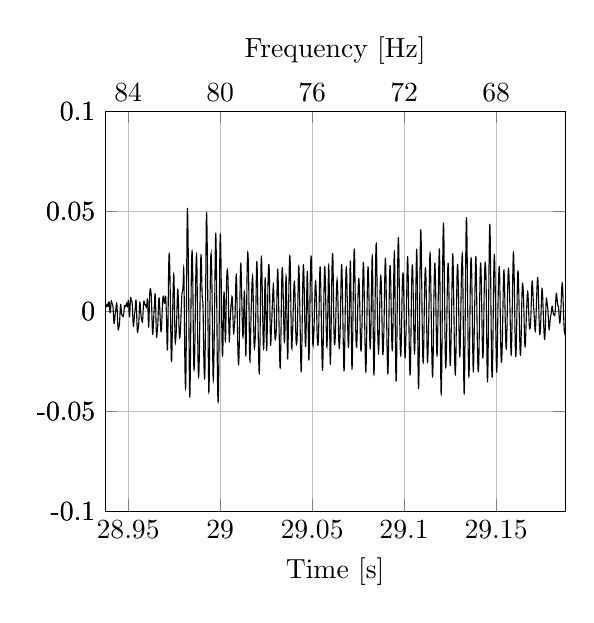
\begin{tikzpicture}


\begin{axis}[%
width=2.3in,
height=2in,
at={(1.011in,0.642in)},
scale only axis,
xmin=28.9375,
xmax=29.1875,
xtick={28.95, 29, 29.05,  29.1, 29.15},
xticklabels={84, 80, 76, 72, 68},
xmajorgrids,
ymin=-0.1,
ymax=0.1,
ymajorgrids,
scaled ticks=false,
ytick={-0.1, -0.05, 0,  0.05, 0.1},
yticklabels={-0.1, -0.05, 0,  0.05, 0.1},
axis x line*=top,
xlabel={Frequency [Hz]},
axis background/.style={fill=white}
]
\end{axis}

\begin{axis}[%
width=2.3in,
height=2in,
at={(1.011in,0.642in)},
scale only axis,
xmin=28.9375,
xmax=29.1875,
xmajorgrids,
ymin=-0.1,
ymax=0.1,
ymajorgrids,
scaled ticks=false,
ytick={-0.1, -0.05, 0,  0.05, 0.1},
yticklabels={-0.1, -0.05, 0,  0.05, 0.1},
xlabel={Time [s]},
axis background/.style={fill=white}
]
\addplot [color=black,solid,forget plot]
table[row sep=crcr]{%
	28.9374791666667	0.00120449066162109\\
	28.9375	0.0013422966003418\\
	28.9375208333333	0.00147902965545654\\
	28.9375416666667	0.00158834457397461\\
	28.9375625	0.00170481204986572\\
	28.9375833333333	0.00182092189788818\\
	28.9376041666667	0.00190639495849609\\
	28.937625	0.00197184085845947\\
	28.9376458333333	0.00206494331359863\\
	28.9376666666667	0.00211882591247559\\
	28.9376875	0.00217843055725098\\
	28.9377083333333	0.00219666957855225\\
	28.9377291666667	0.00223839282989502\\
	28.93775	0.00232481956481934\\
	28.9377708333333	0.00233364105224609\\
	28.9377916666667	0.00235855579376221\\
	28.9378125	0.00237452983856201\\
	28.9378333333333	0.00237023830413818\\
	28.9378541666667	0.00236904621124268\\
	28.937875	0.0023728609085083\\
	28.9378958333333	0.00235486030578613\\
	28.9379166666667	0.00235366821289063\\
	28.9379375	0.00235486030578613\\
	28.9379583333333	0.00233364105224609\\
	28.9379791666667	0.00234019756317139\\
	28.938	0.00231480598449707\\
	28.9380208333333	0.00231778621673584\\
	28.9380416666667	0.00233066082000732\\
	28.9380625	0.00229394435882568\\
	28.9380833333333	0.00233161449432373\\
	28.9381041666667	0.00232195854187012\\
	28.938125	0.00232744216918945\\
	28.9381458333333	0.00236666202545166\\
	28.9381666666667	0.00239074230194092\\
	28.9381875	0.0024111270904541\\
	28.9382083333333	0.00241708755493164\\
	28.9382291666667	0.00250089168548584\\
	28.93825	0.00255060195922852\\
	28.9382708333333	0.00261783599853516\\
	28.9382916666667	0.00265705585479736\\
	28.9383125	0.00270915031433105\\
	28.9383333333333	0.00275206565856934\\
	28.9383541666667	0.00282132625579834\\
	28.938375	0.00291812419891357\\
	28.9383958333333	0.00299406051635742\\
	28.9384166666667	0.00303125381469727\\
	28.9384375	0.00311172008514404\\
	28.9384583333333	0.00321066379547119\\
	28.9384791666667	0.0032811164855957\\
	28.9385	0.00332748889923096\\
	28.9385208333333	0.00336956977844238\\
	28.9385416666667	0.00345480442047119\\
	28.9385625	0.00349807739257813\\
	28.9385833333333	0.00352728366851807\\
	28.9386041666667	0.0035477876663208\\
	28.938625	0.0035707950592041\\
	28.9386458333333	0.00359570980072021\\
	28.9386666666667	0.0036003589630127\\
	28.9386875	0.00357067584991455\\
	28.9387083333333	0.00353062152862549\\
	28.9387291666667	0.00348305702209473\\
	28.93875	0.00348186492919922\\
	28.9387708333333	0.0034555196762085\\
	28.9387916666667	0.00335538387298584\\
	28.9388125	0.00326108932495117\\
	28.9388333333333	0.00318527221679688\\
	28.9388541666667	0.00317442417144775\\
	28.938875	0.00306880474090576\\
	28.9388958333333	0.00293564796447754\\
	28.9389166666667	0.00287473201751709\\
	28.9389375	0.00280296802520752\\
	28.9389583333333	0.00272119045257568\\
	28.9389791666667	0.00266194343566895\\
	28.939	0.00259816646575928\\
	28.9390208333333	0.0025409460067749\\
	28.9390416666667	0.00249350070953369\\
	28.9390625	0.00247383117675781\\
	28.9390833333333	0.00246036052703857\\
	28.9391041666667	0.00245332717895508\\
	28.939125	0.00244832038879395\\
	28.9391458333333	0.00248098373413086\\
	28.9391666666667	0.00252044200897217\\
	28.9391875	0.00253975391387939\\
	28.9392083333333	0.00264823436737061\\
	28.9392291666667	0.00271797180175781\\
	28.93925	0.00281059741973877\\
	28.9392708333333	0.00290811061859131\\
	28.9392916666667	0.00302028656005859\\
	28.9393125	0.00315308570861816\\
	28.9393333333333	0.00329148769378662\\
	28.9393541666667	0.00340831279754639\\
	28.939375	0.00356948375701904\\
	28.9393958333333	0.00372171401977539\\
	28.9394166666667	0.00384736061096191\\
	28.9394375	0.0039832592010498\\
	28.9394583333333	0.00412929058074951\\
	28.9394791666667	0.00424027442932129\\
	28.9395	0.00433218479156494\\
	28.9395208333333	0.00442314147949219\\
	28.9395416666667	0.00449824333190918\\
	28.9395625	0.00455284118652344\\
	28.9395833333333	0.00458669662475586\\
	28.9396041666667	0.0046314001083374\\
	28.939625	0.00459587574005127\\
	28.9396458333333	0.0045621395111084\\
	28.9396666666667	0.00453615188598633\\
	28.9396875	0.0044330358505249\\
	28.9397083333333	0.00432121753692627\\
	28.9397291666667	0.00419533252716064\\
	28.93975	0.00404250621795654\\
	28.9397708333333	0.00387072563171387\\
	28.9397916666667	0.00365662574768066\\
	28.9398125	0.003456711769104\\
	28.9398333333333	0.00322723388671875\\
	28.9398541666667	0.002982497215271\\
	28.939875	0.00272881984710693\\
	28.9398958333333	0.00249087810516357\\
	28.9399166666667	0.00224483013153076\\
	28.9399375	0.00196731090545654\\
	28.9399583333333	0.00170230865478516\\
	28.9399791666667	0.00142776966094971\\
	28.94	0.00115609169006348\\
	28.9400208333333	0.000885367393493652\\
	28.9400416666667	0.000633358955383301\\
	28.9400625	0.000411391258239746\\
	28.9400833333333	0.000180602073669434\\
	28.9401041666667	-8.34465026855469e-06\\
	28.940125	-0.000194072723388672\\
	28.9401458333333	-0.000409603118896484\\
	28.9401666666667	-0.000522017478942871\\
	28.9401875	-0.000576972961425781\\
	28.9402083333333	-0.000643014907836914\\
	28.9402291666667	-0.000677943229675293\\
	28.94025	-0.000661253929138184\\
	28.9402708333333	-0.000652074813842773\\
	28.9402916666667	-0.000607490539550781\\
	28.9403125	-0.000536084175109863\\
	28.9403333333333	-0.000380039215087891\\
	28.9403541666667	-0.000264167785644531\\
	28.940375	-0.00012516975402832\\
	28.9403958333333	1.87158584594727e-05\\
	28.9404166666667	0.000219106674194336\\
	28.9404375	0.000468611717224121\\
	28.9404583333333	0.000717759132385254\\
	28.9404791666667	0.00103902816772461\\
	28.9405	0.00130844116210938\\
	28.9405208333333	0.00157058238983154\\
	28.9405416666667	0.00185871124267578\\
	28.9405625	0.00217807292938232\\
	28.9405833333333	0.00246882438659668\\
	28.9406041666667	0.0027240514755249\\
	28.940625	0.00297737121582031\\
	28.9406458333333	0.00324654579162598\\
	28.9406666666667	0.00350058078765869\\
	28.9406875	0.00375759601593018\\
	28.9407083333333	0.0039670467376709\\
	28.9407291666667	0.00423252582550049\\
	28.94075	0.00441229343414307\\
	28.9407708333333	0.00458657741546631\\
	28.9407916666667	0.00479030609130859\\
	28.9408125	0.00493013858795166\\
	28.9408333333333	0.00502967834472656\\
	28.9408541666667	0.00513112545013428\\
	28.940875	0.00521993637084961\\
	28.9408958333333	0.00522971153259277\\
	28.9409166666667	0.00522172451019287\\
	28.9409375	0.00522911548614502\\
	28.9409583333333	0.00523996353149414\\
	28.9409791666667	0.0052112340927124\\
	28.941	0.00512528419494629\\
	28.9410208333333	0.00503182411193848\\
	28.9410416666667	0.00497424602508545\\
	28.9410625	0.00487077236175537\\
	28.9410833333333	0.00477099418640137\\
	28.9411041666667	0.00464916229248047\\
	28.941125	0.004547119140625\\
	28.9411458333333	0.00443184375762939\\
	28.9411666666667	0.00429177284240723\\
	28.9411875	0.00418353080749512\\
	28.9412083333333	0.00412440299987793\\
	28.9412291666667	0.00401580333709717\\
	28.94125	0.00392568111419678\\
	28.9412708333333	0.00388896465301514\\
	28.9412916666667	0.0037989616394043\\
	28.9413125	0.00372517108917236\\
	28.9413333333333	0.00367295742034912\\
	28.9413541666667	0.00364494323730469\\
	28.941375	0.00362873077392578\\
	28.9413958333333	0.00360417366027832\\
	28.9414166666667	0.00356161594390869\\
	28.9414375	0.00357687473297119\\
	28.9414583333333	0.00352346897125244\\
	28.9414791666667	0.00348567962646484\\
	28.9415	0.00347518920898438\\
	28.9415208333333	0.00347352027893066\\
	28.9415416666667	0.00342643260955811\\
	28.9415625	0.00337326526641846\\
	28.9415833333333	0.00334906578063965\\
	28.9416041666667	0.00328314304351807\\
	28.941625	0.00321304798126221\\
	28.9416458333333	0.00310385227203369\\
	28.9416666666667	0.0030217170715332\\
	28.9416875	0.00289404392242432\\
	28.9417083333333	0.00277328491210938\\
	28.9417291666667	0.00259971618652344\\
	28.94175	0.00243127346038818\\
	28.9417708333333	0.00223422050476074\\
	28.9417916666667	0.00204789638519287\\
	28.9418125	0.00179445743560791\\
	28.9418333333333	0.00156998634338379\\
	28.9418541666667	0.00131797790527344\\
	28.941875	0.00100135803222656\\
	28.9418958333333	0.000730276107788086\\
	28.9419166666667	0.000393033027648926\\
	28.9419375	4.80413436889648e-05\\
	28.9419583333333	-0.000273346900939941\\
	28.9419791666667	-0.000638008117675781\\
	28.942	-0.000986218452453613\\
	28.9420208333333	-0.0013500452041626\\
	28.9420416666667	-0.00172805786132813\\
	28.9420625	-0.00209999084472656\\
	28.9420833333333	-0.00245952606201172\\
	28.9421041666667	-0.00283920764923096\\
	28.942125	-0.00321090221405029\\
	28.9421458333333	-0.00355565547943115\\
	28.9421666666667	-0.00390529632568359\\
	28.9421875	-0.00425815582275391\\
	28.9422083333333	-0.00453579425811768\\
	28.9422291666667	-0.00481522083282471\\
	28.94225	-0.00510096549987793\\
	28.9422708333333	-0.00531721115112305\\
	28.9422916666667	-0.00551402568817139\\
	28.9423125	-0.00571227073669434\\
	28.9423333333333	-0.00587165355682373\\
	28.9423541666667	-0.006011962890625\\
	28.942375	-0.00609862804412842\\
	28.9423958333333	-0.00616216659545898\\
	28.9424166666667	-0.0061640739440918\\
	28.9424375	-0.00617873668670654\\
	28.9424583333333	-0.0061715841293335\\
	28.9424791666667	-0.00609982013702393\\
	28.9425	-0.00601935386657715\\
	28.9425208333333	-0.00593757629394531\\
	28.9425416666667	-0.00584173202514648\\
	28.9425625	-0.00566816329956055\\
	28.9425833333333	-0.00552630424499512\\
	28.9426041666667	-0.00535976886749268\\
	28.942625	-0.00518405437469482\\
	28.9426458333333	-0.00501167774200439\\
	28.9426666666667	-0.00480484962463379\\
	28.9426875	-0.00459206104278564\\
	28.9427083333333	-0.004372239112854\\
	28.9427291666667	-0.00415718555450439\\
	28.94275	-0.00394749641418457\\
	28.9427708333333	-0.00370919704437256\\
	28.9427916666667	-0.00349545478820801\\
	28.9428125	-0.00327563285827637\\
	28.9428333333333	-0.00306379795074463\\
	28.9428541666667	-0.00283503532409668\\
	28.942875	-0.00266897678375244\\
	28.9428958333333	-0.00242698192596436\\
	28.9429166666667	-0.00224006175994873\\
	28.9429375	-0.00203025341033936\\
	28.9429583333333	-0.00185549259185791\\
	28.9429791666667	-0.00171148777008057\\
	28.943	-0.00151622295379639\\
	28.9430208333333	-0.00136935710906982\\
	28.9430416666667	-0.00121152400970459\\
	28.9430625	-0.00106132030487061\\
	28.9430833333333	-0.000919103622436523\\
	28.9431041666667	-0.000782370567321777\\
	28.943125	-0.000638723373413086\\
	28.9431458333333	-0.000498175621032715\\
	28.9431666666667	-0.000345945358276367\\
	28.9431875	-0.000230789184570313\\
	28.9432083333333	-8.38041305541992e-05\\
	28.9432291666667	8.63075256347656e-05\\
	28.94325	0.00023949146270752\\
	28.9432708333333	0.000397205352783203\\
	28.9432916666667	0.000530004501342773\\
	28.9433125	0.000728845596313477\\
	28.9433333333333	0.000880002975463867\\
	28.9433541666667	0.00105178356170654\\
	28.943375	0.00125205516815186\\
	28.9433958333333	0.00144445896148682\\
	28.9434166666667	0.00165307521820068\\
	28.9434375	0.00179791450500488\\
	28.9434583333333	0.00201606750488281\\
	28.9434791666667	0.00223231315612793\\
	28.9435	0.00242531299591064\\
	28.9435208333333	0.00262200832366943\\
	28.9435416666667	0.00280725955963135\\
	28.9435625	0.00299155712127686\\
	28.9435833333333	0.00317680835723877\\
	28.9436041666667	0.00332033634185791\\
	28.943625	0.00349819660186768\\
	28.9436458333333	0.00365996360778809\\
	28.9436666666667	0.00376176834106445\\
	28.9436875	0.0038527250289917\\
	28.9437083333333	0.00394964218139648\\
	28.9437291666667	0.00402390956878662\\
	28.94375	0.00402307510375977\\
	28.9437708333333	0.0040431022644043\\
	28.9437916666667	0.00400960445404053\\
	28.9438125	0.00398123264312744\\
	28.9438333333333	0.00387287139892578\\
	28.9438541666667	0.00376808643341064\\
	28.943875	0.0036466121673584\\
	28.9438958333333	0.00343811511993408\\
	28.9439166666667	0.00322556495666504\\
	28.9439375	0.00299918651580811\\
	28.9439583333333	0.00274956226348877\\
	28.9439791666667	0.00238537788391113\\
	28.944	0.00204110145568848\\
	28.9440208333333	0.00170993804931641\\
	28.9440416666667	0.00127840042114258\\
	28.9440625	0.00086820125579834\\
	28.9440833333333	0.00043022632598877\\
	28.9441041666667	-4.25577163696289e-05\\
	28.944125	-0.000528573989868164\\
	28.9441458333333	-0.000995159149169922\\
	28.9441666666667	-0.00151360034942627\\
	28.9441875	-0.00202596187591553\\
	28.9442083333333	-0.00253725051879883\\
	28.9442291666667	-0.00308370590209961\\
	28.94425	-0.00356650352478027\\
	28.9442708333333	-0.00408291816711426\\
	28.9442916666667	-0.00460159778594971\\
	28.9443125	-0.00507307052612305\\
	28.9443333333333	-0.00550568103790283\\
	28.9443541666667	-0.00596094131469727\\
	28.944375	-0.00639355182647705\\
	28.9443958333333	-0.00678336620330811\\
	28.9444166666667	-0.00715458393096924\\
	28.9444375	-0.00749218463897705\\
	28.9444583333333	-0.00781965255737305\\
	28.9444791666667	-0.00808835029602051\\
	28.9445	-0.00832915306091309\\
	28.9445208333333	-0.00857234001159668\\
	28.9445416666667	-0.0087350606918335\\
	28.9445625	-0.00887703895568848\\
	28.9445833333333	-0.00901639461517334\\
	28.9446041666667	-0.00910532474517822\\
	28.944625	-0.00917530059814453\\
	28.9446458333333	-0.00921499729156494\\
	28.9446666666667	-0.00927221775054932\\
	28.9446875	-0.0092463493347168\\
	28.9447083333333	-0.00926792621612549\\
	28.9447291666667	-0.00922989845275879\\
	28.94475	-0.00919866561889648\\
	28.9447708333333	-0.00914144515991211\\
	28.9447916666667	-0.00907063484191895\\
	28.9448125	-0.00901293754577637\\
	28.9448333333333	-0.00892424583435059\\
	28.9448541666667	-0.00883769989013672\\
	28.944875	-0.00875723361968994\\
	28.9448958333333	-0.00870335102081299\\
	28.9449166666667	-0.0085904598236084\\
	28.9449375	-0.00850820541381836\\
	28.9449583333333	-0.00839269161224365\\
	28.9449791666667	-0.00831711292266846\\
	28.945	-0.0082094669342041\\
	28.9450208333333	-0.00813567638397217\\
	28.9450416666667	-0.00805056095123291\\
	28.9450625	-0.0079272985458374\\
	28.9450833333333	-0.00782966613769531\\
	28.9451041666667	-0.0077434778213501\\
	28.945125	-0.00762271881103516\\
	28.9451458333333	-0.00748217105865479\\
	28.9451666666667	-0.0074012279510498\\
	28.9451875	-0.00725114345550537\\
	28.9452083333333	-0.00711047649383545\\
	28.9452291666667	-0.00694930553436279\\
	28.94525	-0.0067903995513916\\
	28.9452708333333	-0.00657689571380615\\
	28.9452916666667	-0.00638699531555176\\
	28.9453125	-0.00614047050476074\\
	28.9453333333333	-0.00589501857757568\\
	28.9453541666667	-0.00564134120941162\\
	28.945375	-0.00533878803253174\\
	28.9453958333333	-0.0050283670425415\\
	28.9454166666667	-0.0046771764755249\\
	28.9454375	-0.0043487548828125\\
	28.9454583333333	-0.00397193431854248\\
	28.9454791666667	-0.00359225273132324\\
	28.9455	-0.00320053100585938\\
	28.9455208333333	-0.00277113914489746\\
	28.9455416666667	-0.00234317779541016\\
	28.9455625	-0.00193297863006592\\
	28.9455833333333	-0.00148999691009521\\
	28.9456041666667	-0.0010521411895752\\
	28.945625	-0.000657558441162109\\
	28.9456458333333	-0.000228643417358398\\
	28.9456666666667	0.000164389610290527\\
	28.9456875	0.000571966171264648\\
	28.9457083333333	0.000959157943725586\\
	28.9457291666667	0.0012742280960083\\
	28.94575	0.00164806842803955\\
	28.9457708333333	0.00197863578796387\\
	28.9457916666667	0.00224733352661133\\
	28.9458125	0.00248706340789795\\
	28.9458333333333	0.00269651412963867\\
	28.9458541666667	0.00291526317596436\\
	28.945875	0.00307631492614746\\
	28.9458958333333	0.00319766998291016\\
	28.9459166666667	0.00328361988067627\\
	28.9459375	0.00333547592163086\\
	28.9459583333333	0.0033566951751709\\
	28.9459791666667	0.00334405899047852\\
	28.946	0.00330209732055664\\
	28.9460208333333	0.00322556495666504\\
	28.9460416666667	0.00311374664306641\\
	28.9460625	0.00297248363494873\\
	28.9460833333333	0.00281548500061035\\
	28.9461041666667	0.00264823436737061\\
	28.946125	0.00243580341339111\\
	28.9461458333333	0.00223219394683838\\
	28.9461666666667	0.00200450420379639\\
	28.9461875	0.00174605846405029\\
	28.9462083333333	0.00149452686309814\\
	28.9462291666667	0.00123834609985352\\
	28.94625	0.000975608825683594\\
	28.9462708333333	0.000711798667907715\\
	28.9462916666667	0.000437259674072266\\
	28.9463125	0.000186920166015625\\
	28.9463333333333	-4.62532043457031e-05\\
	28.9463541666667	-0.000296592712402344\\
	28.946375	-0.000509381294250488\\
	28.9463958333333	-0.000693798065185547\\
	28.9464166666667	-0.000870347023010254\\
	28.9464375	-0.00106263160705566\\
	28.9464583333333	-0.00124084949493408\\
	28.9464791666667	-0.00135302543640137\\
	28.9465	-0.00150108337402344\\
	28.9465208333333	-0.00159585475921631\\
	28.9465416666667	-0.00174951553344727\\
	28.9465625	-0.00178027153015137\\
	28.9465833333333	-0.00185716152191162\\
	28.9466041666667	-0.00190210342407227\\
	28.946625	-0.00194311141967773\\
	28.9466458333333	-0.00195682048797607\\
	28.9466666666667	-0.00200092792510986\\
	28.9466875	-0.00200068950653076\\
	28.9467083333333	-0.00199317932128906\\
	28.9467291666667	-0.00199985504150391\\
	28.94675	-0.00198268890380859\\
	28.9467708333333	-0.00201892852783203\\
	28.9467916666667	-0.00195181369781494\\
	28.9468125	-0.00197136402130127\\
	28.9468333333333	-0.00197088718414307\\
	28.9468541666667	-0.00195300579071045\\
	28.946875	-0.0019221305847168\\
	28.9468958333333	-0.00193166732788086\\
	28.9469166666667	-0.00193977355957031\\
	28.9469375	-0.00197398662567139\\
	28.9469583333333	-0.00198137760162354\\
	28.9469791666667	-0.00202929973602295\\
	28.947	-0.00204813480377197\\
	28.9470208333333	-0.00205314159393311\\
	28.9470416666667	-0.0021357536315918\\
	28.9470625	-0.00214993953704834\\
	28.9470833333333	-0.0022275447845459\\
	28.9471041666667	-0.00226342678070068\\
	28.947125	-0.0023338794708252\\
	28.9471458333333	-0.0023953914642334\\
	28.9471666666667	-0.00243794918060303\\
	28.9471875	-0.00251471996307373\\
	28.9472083333333	-0.00256145000457764\\
	28.9472291666667	-0.00262069702148438\\
	28.94725	-0.00264477729797363\\
	28.9472708333333	-0.00268018245697021\\
	28.9472916666667	-0.00271868705749512\\
	28.9473125	-0.00275373458862305\\
	28.9473333333333	-0.0027240514755249\\
	28.9473541666667	-0.00271487236022949\\
	28.947375	-0.00269734859466553\\
	28.9473958333333	-0.00266361236572266\\
	28.9474166666667	-0.00259816646575928\\
	28.9474375	-0.00254809856414795\\
	28.9474583333333	-0.0024724006652832\\
	28.9474791666667	-0.00236475467681885\\
	28.9475	-0.00222373008728027\\
	28.9475208333333	-0.00209498405456543\\
	28.9475416666667	-0.00199651718139648\\
	28.9475625	-0.00181496143341064\\
	28.9475833333333	-0.00161874294281006\\
	28.9476041666667	-0.00142979621887207\\
	28.947625	-0.00125586986541748\\
	28.9476458333333	-0.00103628635406494\\
	28.9476666666667	-0.00085151195526123\\
	28.9476875	-0.000629663467407227\\
	28.9477083333333	-0.000427961349487305\\
	28.9477291666667	-0.000189900398254395\\
	28.94775	2.43186950683594e-05\\
	28.9477708333333	0.000212907791137695\\
	28.9477916666667	0.000438451766967773\\
	28.9478125	0.000701308250427246\\
	28.9478333333333	0.000888824462890625\\
	28.9478541666667	0.00107264518737793\\
	28.947875	0.00127303600311279\\
	28.9478958333333	0.00148415565490723\\
	28.9479166666667	0.00163650512695313\\
	28.9479375	0.00178205966949463\\
	28.9479583333333	0.0019611120223999\\
	28.9479791666667	0.00208234786987305\\
	28.948	0.0022122859954834\\
	28.9480208333333	0.00233030319213867\\
	28.9480416666667	0.00245213508605957\\
	28.9480625	0.00254130363464355\\
	28.9480833333333	0.00261390209197998\\
	28.9481041666667	0.00266730785369873\\
	28.948125	0.002768874168396\\
	28.9481458333333	0.00282394886016846\\
	28.9481666666667	0.00283098220825195\\
	28.9481875	0.00286483764648438\\
	28.9482083333333	0.00290322303771973\\
	28.9482291666667	0.00289678573608398\\
	28.94825	0.0028834342956543\\
	28.9482708333333	0.00288903713226318\\
	28.9482916666667	0.00288474559783936\\
	28.9483125	0.00286269187927246\\
	28.9483333333333	0.00282883644104004\\
	28.9483541666667	0.00279414653778076\\
	28.948375	0.00276303291320801\\
	28.9483958333333	0.00272870063781738\\
	28.9484166666667	0.00271797180175781\\
	28.9484375	0.00267577171325684\\
	28.9484583333333	0.00263571739196777\\
	28.9484791666667	0.00257432460784912\\
	28.9485	0.00260186195373535\\
	28.9485208333333	0.00261199474334717\\
	28.9485416666667	0.0025259256362915\\
	28.9485625	0.00253629684448242\\
	28.9485833333333	0.00254309177398682\\
	28.9486041666667	0.00254881381988525\\
	28.948625	0.00251924991607666\\
	28.9486458333333	0.00258731842041016\\
	28.9486666666667	0.0026010274887085\\
	28.9486875	0.00260651111602783\\
	28.9487083333333	0.00261986255645752\\
	28.9487291666667	0.00269746780395508\\
	28.94875	0.00275719165802002\\
	28.9487708333333	0.00278258323669434\\
	28.9487916666667	0.00282752513885498\\
	28.9488125	0.00287473201751709\\
	28.9488333333333	0.00293600559234619\\
	28.9488541666667	0.00301527976989746\\
	28.948875	0.0030893087387085\\
	28.9488958333333	0.00317025184631348\\
	28.9489166666667	0.00324559211730957\\
	28.9489375	0.00328946113586426\\
	28.9489583333333	0.00333797931671143\\
	28.9489791666667	0.00340175628662109\\
	28.949	0.00345754623413086\\
	28.9490208333333	0.00350940227508545\\
	28.9490416666667	0.00359416007995605\\
	28.9490625	0.00362908840179443\\
	28.9490833333333	0.00361824035644531\\
	28.9491041666667	0.0036015510559082\\
	28.949125	0.00365960597991943\\
	28.9491458333333	0.00370883941650391\\
	28.9491666666667	0.00361740589141846\\
	28.9491875	0.00354647636413574\\
	28.9492083333333	0.00355947017669678\\
	28.9492291666667	0.00348484516143799\\
	28.94925	0.00344514846801758\\
	28.9492708333333	0.00336253643035889\\
	28.9492916666667	0.00326979160308838\\
	28.9493125	0.00314474105834961\\
	28.9493333333333	0.00303030014038086\\
	28.9493541666667	0.00299572944641113\\
	28.949375	0.00288474559783936\\
	28.9493958333333	0.00273466110229492\\
	28.9494166666667	0.00265610218048096\\
	28.9494375	0.00257062911987305\\
	28.9494583333333	0.00245749950408936\\
	28.9494791666667	0.00238919258117676\\
	28.9495	0.00232481956481934\\
	28.9495208333333	0.00229990482330322\\
	28.9495416666667	0.00223338603973389\\
	28.9495625	0.002205491065979\\
	28.9495833333333	0.00222384929656982\\
	28.9496041666667	0.00224018096923828\\
	28.949625	0.00226807594299316\\
	28.9496458333333	0.002349853515625\\
	28.9496666666667	0.00245094299316406\\
	28.9496875	0.00250637531280518\\
	28.9497083333333	0.0025869607925415\\
	28.9497291666667	0.00275886058807373\\
	28.94975	0.00294363498687744\\
	28.9497708333333	0.00306534767150879\\
	28.9497916666667	0.00320351123809814\\
	28.9498125	0.00345981121063232\\
	28.9498333333333	0.00364840030670166\\
	28.9498541666667	0.00382018089294434\\
	28.949875	0.00399625301361084\\
	28.9498958333333	0.00420570373535156\\
	28.9499166666667	0.00439226627349854\\
	28.9499375	0.00453698635101318\\
	28.9499583333333	0.0047307014465332\\
	28.9499791666667	0.00490379333496094\\
	28.95	0.00499629974365234\\
	28.9500208333333	0.00507068634033203\\
	28.9500416666667	0.00517380237579346\\
	28.9500625	0.00527513027191162\\
	28.9500833333333	0.00526750087738037\\
	28.9501041666667	0.00522792339324951\\
	28.950125	0.00524055957794189\\
	28.9501458333333	0.00517702102661133\\
	28.9501666666667	0.00502884387969971\\
	28.9501875	0.00488781929016113\\
	28.9502083333333	0.00475656986236572\\
	28.9502291666667	0.00458204746246338\\
	28.95025	0.00433135032653809\\
	28.9502708333333	0.00405228137969971\\
	28.9502916666667	0.00383269786834717\\
	28.9503125	0.00350522994995117\\
	28.9503333333333	0.00316107273101807\\
	28.9503541666667	0.00278890132904053\\
	28.950375	0.00247848033905029\\
	28.9503958333333	0.00213134288787842\\
	28.9504166666667	0.0016934871673584\\
	28.9504375	0.00128757953643799\\
	28.9504583333333	0.000902414321899414\\
	28.9504791666667	0.000477790832519531\\
	28.9505	3.38554382324219e-05\\
	28.9505208333333	-0.000324130058288574\\
	28.9505416666667	-0.000696778297424316\\
	28.9505625	-0.00110518932342529\\
	28.9505833333333	-0.00148618221282959\\
	28.9506041666667	-0.0017240047454834\\
	28.950625	-0.00196230411529541\\
	28.9506458333333	-0.00223922729492188\\
	28.9506666666667	-0.00240206718444824\\
	28.9506875	-0.00247740745544434\\
	28.9507083333333	-0.00260722637176514\\
	28.9507291666667	-0.00270664691925049\\
	28.95075	-0.00269615650177002\\
	28.9507708333333	-0.00262069702148438\\
	28.9507916666667	-0.00257313251495361\\
	28.9508125	-0.0025097131729126\\
	28.9508333333333	-0.00235104560852051\\
	28.9508541666667	-0.00208103656768799\\
	28.950875	-0.00179779529571533\\
	28.9508958333333	-0.00150954723358154\\
	28.9509166666667	-0.00117194652557373\\
	28.9509375	-0.000782370567321777\\
	28.9509583333333	-0.00044858455657959\\
	28.9509791666667	-8.34465026855469e-05\\
	28.951	0.000378012657165527\\
	28.9510208333333	0.000835776329040527\\
	28.9510416666667	0.00127923488616943\\
	28.9510625	0.00171661376953125\\
	28.9510833333333	0.00211620330810547\\
	28.9511041666667	0.00249087810516357\\
	28.951125	0.00293815135955811\\
	28.9511458333333	0.00336539745330811\\
	28.9511666666667	0.00378096103668213\\
	28.9511875	0.00420570373535156\\
	28.9512083333333	0.004599928855896\\
	28.9512291666667	0.00494003295898438\\
	28.95125	0.00526010990142822\\
	28.9512708333333	0.00555706024169922\\
	28.9512916666667	0.00581920146942139\\
	28.9513125	0.00606405735015869\\
	28.9513333333333	0.0062861442565918\\
	28.9513541666667	0.00645327568054199\\
	28.951375	0.00657689571380615\\
	28.9513958333333	0.00669670104980469\\
	28.9514166666667	0.00680875778198242\\
	28.9514375	0.00682854652404785\\
	28.9514583333333	0.00684773921966553\\
	28.9514791666667	0.00681555271148682\\
	28.9515	0.00680291652679443\\
	28.9515208333333	0.00669407844543457\\
	28.9515416666667	0.00658977031707764\\
	28.9515625	0.00653398036956787\\
	28.9515833333333	0.00641906261444092\\
	28.9516041666667	0.00633645057678223\\
	28.951625	0.0062251091003418\\
	28.9516458333333	0.00611782073974609\\
	28.9516666666667	0.00599849224090576\\
	28.9516875	0.00585758686065674\\
	28.9517083333333	0.00576698780059814\\
	28.9517291666667	0.00570058822631836\\
	28.95175	0.00557601451873779\\
	28.9517708333333	0.00548863410949707\\
	28.9517916666667	0.00545024871826172\\
	28.9518125	0.00538110733032227\\
	28.9518333333333	0.0052955150604248\\
	28.9518541666667	0.0052649974822998\\
	28.951875	0.00523805618286133\\
	28.9518958333333	0.00520634651184082\\
	28.9519166666667	0.0051729679107666\\
	28.9519375	0.00515663623809814\\
	28.9519583333333	0.00512909889221191\\
	28.9519791666667	0.00505387783050537\\
	28.952	0.00503396987915039\\
	28.9520208333333	0.0050126314163208\\
	28.9520416666667	0.00497937202453613\\
	28.9520625	0.00488507747650146\\
	28.9520833333333	0.00477564334869385\\
	28.9521041666667	0.00469386577606201\\
	28.952125	0.00460553169250488\\
	28.9521458333333	0.00447690486907959\\
	28.9521666666667	0.00430679321289063\\
	28.9521875	0.00413095951080322\\
	28.9522083333333	0.00396382808685303\\
	28.9522291666667	0.00372219085693359\\
	28.95225	0.00348925590515137\\
	28.9522708333333	0.00323283672332764\\
	28.9522916666667	0.00292778015136719\\
	28.9523125	0.00257265567779541\\
	28.9523333333333	0.00225222110748291\\
	28.9523541666667	0.00188350677490234\\
	28.952375	0.00146079063415527\\
	28.9523958333333	0.00111985206604004\\
	28.9524166666667	0.000669598579406738\\
	28.9524375	0.000219464302062988\\
	28.9524583333333	-0.000203490257263184\\
	28.9524791666667	-0.000688910484313965\\
	28.9525	-0.00115406513214111\\
	28.9525208333333	-0.00164473056793213\\
	28.9525416666667	-0.00214004516601563\\
	28.9525625	-0.00266695022583008\\
	28.9525833333333	-0.00313663482666016\\
	28.9526041666667	-0.00356113910675049\\
	28.952625	-0.00401782989501953\\
	28.9526458333333	-0.00445592403411865\\
	28.9526666666667	-0.00490152835845947\\
	28.9526875	-0.00530540943145752\\
	28.9527083333333	-0.00565338134765625\\
	28.9527291666667	-0.0059959888458252\\
	28.95275	-0.00635015964508057\\
	28.9527708333333	-0.00661516189575195\\
	28.9527916666667	-0.00686180591583252\\
	28.9528125	-0.00709497928619385\\
	28.9528333333333	-0.00728070735931396\\
	28.9528541666667	-0.00741219520568848\\
	28.952875	-0.00749480724334717\\
	28.9528958333333	-0.00756931304931641\\
	28.9529166666667	-0.00758779048919678\\
	28.9529375	-0.00757312774658203\\
	28.9529583333333	-0.00751519203186035\\
	28.9529791666667	-0.00745391845703125\\
	28.953	-0.00731074810028076\\
	28.9530208333333	-0.00720894336700439\\
	28.9530416666667	-0.00704288482666016\\
	28.9530625	-0.00687050819396973\\
	28.9530833333333	-0.00668728351593018\\
	28.9531041666667	-0.00647926330566406\\
	28.953125	-0.00625467300415039\\
	28.9531458333333	-0.00600981712341309\\
	28.9531666666667	-0.00573980808258057\\
	28.9531875	-0.00549042224884033\\
	28.9532083333333	-0.0052182674407959\\
	28.9532291666667	-0.00494956970214844\\
	28.95325	-0.00468552112579346\\
	28.9532708333333	-0.00440812110900879\\
	28.9532916666667	-0.00417304039001465\\
	28.9533125	-0.00392496585845947\\
	28.9533333333333	-0.00367546081542969\\
	28.9533541666667	-0.00341963768005371\\
	28.953375	-0.00317132472991943\\
	28.9533958333333	-0.00293517112731934\\
	28.9534166666667	-0.00268399715423584\\
	28.9534375	-0.00247335433959961\\
	28.9534583333333	-0.00228261947631836\\
	28.9534791666667	-0.00204145908355713\\
	28.9535	-0.00187921524047852\\
	28.9535208333333	-0.00170278549194336\\
	28.9535416666667	-0.00151956081390381\\
	28.9535625	-0.00134849548339844\\
	28.9535833333333	-0.00116229057312012\\
	28.9536041666667	-0.00100100040435791\\
	28.953625	-0.000794291496276855\\
	28.9536458333333	-0.000609517097473145\\
	28.9536666666667	-0.000457167625427246\\
	28.9536875	-0.000290870666503906\\
	28.9537083333333	-6.79492950439453e-05\\
	28.9537291666667	0.000105500221252441\\
	28.95375	0.000274181365966797\\
	28.9537708333333	0.000500321388244629\\
	28.9537916666667	0.000700950622558594\\
	28.9538125	0.000948309898376465\\
	28.9538333333333	0.00116086006164551\\
	28.9538541666667	0.0013805627822876\\
	28.953875	0.00164890289306641\\
	28.9538958333333	0.00190436840057373\\
	28.9539166666667	0.00211906433105469\\
	28.9539375	0.00242495536804199\\
	28.9539583333333	0.00268375873565674\\
	28.9539791666667	0.00295066833496094\\
	28.954	0.00319314002990723\\
	28.9540208333333	0.00344312191009521\\
	28.9540416666667	0.00373101234436035\\
	28.9540625	0.00397837162017822\\
	28.9540833333333	0.00425004959106445\\
	28.9541041666667	0.00446522235870361\\
	28.954125	0.0046539306640625\\
	28.9541458333333	0.0048515796661377\\
	28.9541666666667	0.00503635406494141\\
	28.9541875	0.00519454479217529\\
	28.9542083333333	0.00532019138336182\\
	28.9542291666667	0.00537395477294922\\
	28.95425	0.00546491146087646\\
	28.9542708333333	0.00549256801605225\\
	28.9542916666667	0.00544416904449463\\
	28.9543125	0.00538980960845947\\
	28.9543333333333	0.00531816482543945\\
	28.9543541666667	0.00517880916595459\\
	28.954375	0.0049821138381958\\
	28.9543958333333	0.00475597381591797\\
	28.9544166666667	0.00447738170623779\\
	28.9544375	0.00416076183319092\\
	28.9544583333333	0.00379776954650879\\
	28.9544791666667	0.00340592861175537\\
	28.9545	0.00294911861419678\\
	28.9545208333333	0.00252604484558105\\
	28.9545416666667	0.00204122066497803\\
	28.9545625	0.00148046016693115\\
	28.9545833333333	0.000900387763977051\\
	28.9546041666667	0.000314235687255859\\
	28.954625	-0.000279426574707031\\
	28.9546458333333	-0.000893354415893555\\
	28.9546666666667	-0.00152122974395752\\
	28.9546875	-0.00219964981079102\\
	28.9547083333333	-0.00283873081207275\\
	28.9547291666667	-0.0034942626953125\\
	28.95475	-0.00412964820861816\\
	28.9547708333333	-0.00474798679351807\\
	28.9547916666667	-0.00536942481994629\\
	28.9548125	-0.00594055652618408\\
	28.9548333333333	-0.00648868083953857\\
	28.9548541666667	-0.00704109668731689\\
	28.954875	-0.00754189491271973\\
	28.9548958333333	-0.00797832012176514\\
	28.9549166666667	-0.00843691825866699\\
	28.9549375	-0.00882446765899658\\
	28.9549583333333	-0.00917530059814453\\
	28.9549791666667	-0.00946581363677979\\
	28.955	-0.00973606109619141\\
	28.9550208333333	-0.00999271869659424\\
	28.9550416666667	-0.0101704597473145\\
	28.9550625	-0.0103230476379395\\
	28.9550833333333	-0.0104254484176636\\
	28.9551041666667	-0.0105032920837402\\
	28.955125	-0.0105493068695068\\
	28.9551458333333	-0.0105750560760498\\
	28.9551666666667	-0.0105768442153931\\
	28.9551875	-0.0105404853820801\\
	28.9552083333333	-0.0104724168777466\\
	28.9552291666667	-0.0103836059570313\\
	28.95525	-0.010285496711731\\
	28.9552708333333	-0.0101571083068848\\
	28.9552916666667	-0.0100215673446655\\
	28.9553125	-0.00990748405456543\\
	28.9553333333333	-0.00978660583496094\\
	28.9553541666667	-0.00964224338531494\\
	28.955375	-0.0095217227935791\\
	28.9553958333333	-0.00938808917999268\\
	28.9554166666667	-0.0092320442199707\\
	28.9554375	-0.00913023948669434\\
	28.9554583333333	-0.00894427299499512\\
	28.9554791666667	-0.00882101058959961\\
	28.9555	-0.0086979866027832\\
	28.9555208333333	-0.00857293605804443\\
	28.9555416666667	-0.00847065448760986\\
	28.9555625	-0.00832951068878174\\
	28.9555833333333	-0.0082094669342041\\
	28.9556041666667	-0.00808465480804443\\
	28.955625	-0.00793445110321045\\
	28.9556458333333	-0.00778770446777344\\
	28.9556666666667	-0.0076291561126709\\
	28.9556875	-0.00744998455047607\\
	28.9557083333333	-0.00727570056915283\\
	28.9557291666667	-0.00702822208404541\\
	28.95575	-0.00678634643554688\\
	28.9557708333333	-0.00655519962310791\\
	28.9557916666667	-0.00625503063201904\\
	28.9558125	-0.00593018531799316\\
	28.9558333333333	-0.00559592247009277\\
	28.9558541666667	-0.00524747371673584\\
	28.955875	-0.00481438636779785\\
	28.9558958333333	-0.0044022798538208\\
	28.9559166666667	-0.0039752721786499\\
	28.9559375	-0.00349390506744385\\
	28.9559583333333	-0.00299704074859619\\
	28.9559791666667	-0.00252139568328857\\
	28.956	-0.00204360485076904\\
	28.9560208333333	-0.00151491165161133\\
	28.9560416666667	-0.00101673603057861\\
	28.9560625	-0.000505208969116211\\
	28.9560833333333	-7.15255737304688e-07\\
	28.9561041666667	0.000502347946166992\\
	28.956125	0.000982284545898438\\
	28.9561458333333	0.00147163867950439\\
	28.9561666666667	0.00189208984375\\
	28.9561875	0.00230145454406738\\
	28.9562083333333	0.00271952152252197\\
	28.9562291666667	0.00310266017913818\\
	28.95625	0.00342249870300293\\
	28.9562708333333	0.00370335578918457\\
	28.9562916666667	0.00393462181091309\\
	28.9563125	0.00415194034576416\\
	28.9563333333333	0.00431013107299805\\
	28.9563541666667	0.00444197654724121\\
	28.956375	0.00454044342041016\\
	28.9563958333333	0.00458753108978271\\
	28.9564166666667	0.0045846700668335\\
	28.9564375	0.00454378128051758\\
	28.9564583333333	0.00447869300842285\\
	28.9564791666667	0.00437462329864502\\
	28.9565	0.00427126884460449\\
	28.9565208333333	0.00410723686218262\\
	28.9565416666667	0.00391364097595215\\
	28.9565625	0.00366950035095215\\
	28.9565833333333	0.00344395637512207\\
	28.9566041666667	0.00315606594085693\\
	28.956625	0.0028681755065918\\
	28.9566458333333	0.00257217884063721\\
	28.9566666666667	0.00225400924682617\\
	28.9566875	0.00198066234588623\\
	28.9567083333333	0.00165057182312012\\
	28.9567291666667	0.00133812427520752\\
	28.95675	0.00105643272399902\\
	28.9567708333333	0.000751376152038574\\
	28.9567916666667	0.000424861907958984\\
	28.9568125	0.000171065330505371\\
	28.9568333333333	-9.0479850769043e-05\\
	28.9568541666667	-0.000412583351135254\\
	28.956875	-0.000677227973937988\\
	28.9568958333333	-0.000899434089660645\\
	28.9569166666667	-0.00112056732177734\\
	28.9569375	-0.00137567520141602\\
	28.9569583333333	-0.00157546997070313\\
	28.9569791666667	-0.00175034999847412\\
	28.957	-0.00192892551422119\\
	28.9570208333333	-0.00210666656494141\\
	28.9570416666667	-0.00226378440856934\\
	28.9570625	-0.00239062309265137\\
	28.9570833333333	-0.00253975391387939\\
	28.9571041666667	-0.00269770622253418\\
	28.957125	-0.00281667709350586\\
	28.9571458333333	-0.0028921365737915\\
	28.9571666666667	-0.00301814079284668\\
	28.9571875	-0.00316214561462402\\
	28.9572083333333	-0.00325405597686768\\
	28.9572291666667	-0.00332438945770264\\
	28.95725	-0.00347423553466797\\
	28.9572708333333	-0.00358736515045166\\
	28.9572916666667	-0.00364816188812256\\
	28.9573125	-0.00376880168914795\\
	28.9573333333333	-0.00388860702514648\\
	28.9573541666667	-0.00401592254638672\\
	28.957375	-0.00411760807037354\\
	28.9573958333333	-0.00422906875610352\\
	28.9574166666667	-0.00434303283691406\\
	28.9574375	-0.00446224212646484\\
	28.9574583333333	-0.00459122657775879\\
	28.9574791666667	-0.00470340251922607\\
	28.9575	-0.00483143329620361\\
	28.9575208333333	-0.00491082668304443\\
	28.9575416666667	-0.00500977039337158\\
	28.9575625	-0.00514519214630127\\
	28.9575833333333	-0.0052182674407959\\
	28.9576041666667	-0.00528013706207275\\
	28.957625	-0.00533974170684814\\
	28.9576458333333	-0.00541150569915771\\
	28.9576666666667	-0.0054318904876709\\
	28.9576875	-0.00544106960296631\\
	28.9577083333333	-0.00546121597290039\\
	28.9577291666667	-0.00540852546691895\\
	28.95775	-0.00538194179534912\\
	28.9577708333333	-0.0053030252456665\\
	28.9577916666667	-0.00520288944244385\\
	28.9578125	-0.00511598587036133\\
	28.9578333333333	-0.00496828556060791\\
	28.9578541666667	-0.00479567050933838\\
	28.957875	-0.00462913513183594\\
	28.9578958333333	-0.00439846515655518\\
	28.9579166666667	-0.00417149066925049\\
	28.9579375	-0.00386989116668701\\
	28.9579583333333	-0.00359725952148438\\
	28.9579791666667	-0.00328981876373291\\
	28.958	-0.0029522180557251\\
	28.9580208333333	-0.00262069702148438\\
	28.9580416666667	-0.00224769115447998\\
	28.9580625	-0.00188589096069336\\
	28.9580833333333	-0.0014883279800415\\
	28.9581041666667	-0.00112724304199219\\
	28.958125	-0.000753998756408691\\
	28.9581458333333	-0.000306248664855957\\
	28.9581666666667	8.85725021362305e-05\\
	28.9581875	0.000467658042907715\\
	28.9582083333333	0.000868678092956543\\
	28.9582291666667	0.00126349925994873\\
	28.95825	0.00159382820129395\\
	28.9582708333333	0.00193023681640625\\
	28.9582916666667	0.0022960901260376\\
	28.9583125	0.00263822078704834\\
	28.9583333333333	0.00293898582458496\\
	28.9583541666667	0.00319647789001465\\
	28.958375	0.00343501567840576\\
	28.9583958333333	0.00368666648864746\\
	28.9584166666667	0.0039290189743042\\
	28.9584375	0.00411438941955566\\
	28.9584583333333	0.00428915023803711\\
	28.9584791666667	0.00444447994232178\\
	28.9585	0.00455582141876221\\
	28.9585208333333	0.00466132164001465\\
	28.9585416666667	0.00477266311645508\\
	28.9585625	0.00482368469238281\\
	28.9585833333333	0.00485706329345703\\
	28.9586041666667	0.00491297245025635\\
	28.958625	0.00495719909667969\\
	28.9586458333333	0.00490915775299072\\
	28.9586666666667	0.00486946105957031\\
	28.9586875	0.00485026836395264\\
	28.9587083333333	0.00480246543884277\\
	28.9587291666667	0.00474405288696289\\
	28.95875	0.00468635559082031\\
	28.9587708333333	0.00462841987609863\\
	28.9587916666667	0.00449824333190918\\
	28.9588125	0.00438845157623291\\
	28.9588333333333	0.00435793399810791\\
	28.9588541666667	0.00428080558776855\\
	28.958875	0.0041424036026001\\
	28.9588958333333	0.00405645370483398\\
	28.9589166666667	0.00400471687316895\\
	28.9589375	0.00390815734863281\\
	28.9589583333333	0.00382733345031738\\
	28.9589791666667	0.00376176834106445\\
	28.959	0.00368845462799072\\
	28.9590208333333	0.00362837314605713\\
	28.9590416666667	0.00353908538818359\\
	28.9590625	0.00352597236633301\\
	28.9590833333333	0.00348150730133057\\
	28.9591041666667	0.00338888168334961\\
	28.959125	0.00334370136260986\\
	28.9591458333333	0.00332820415496826\\
	28.9591666666667	0.00326156616210938\\
	28.9591875	0.00322854518890381\\
	28.9592083333333	0.00319218635559082\\
	28.9592291666667	0.00316357612609863\\
	28.95925	0.0031430721282959\\
	28.9592708333333	0.00309181213378906\\
	28.9592916666667	0.00307798385620117\\
	28.9593125	0.00307083129882813\\
	28.9593333333333	0.00307929515838623\\
	28.9593541666667	0.00302028656005859\\
	28.959375	0.00298082828521729\\
	28.9593958333333	0.00300610065460205\\
	28.9594166666667	0.00300836563110352\\
	28.9594375	0.00296783447265625\\
	28.9594583333333	0.00297856330871582\\
	28.9594791666667	0.00301039218902588\\
	28.9595	0.00296151638031006\\
	28.9595208333333	0.00294613838195801\\
	28.9595416666667	0.00297081470489502\\
	28.9595625	0.00295579433441162\\
	28.9595833333333	0.00286734104156494\\
	28.9596041666667	0.0028759241104126\\
	28.959625	0.00288176536560059\\
	28.9596458333333	0.00281000137329102\\
	28.9596666666667	0.00275087356567383\\
	28.9596875	0.00270700454711914\\
	28.9597083333333	0.00270462036132813\\
	28.9597291666667	0.0026094913482666\\
	28.95975	0.00251424312591553\\
	28.9597708333333	0.00248515605926514\\
	28.9597916666667	0.00244176387786865\\
	28.9598125	0.00230515003204346\\
	28.9598333333333	0.00226759910583496\\
	28.9598541666667	0.00228989124298096\\
	28.959875	0.00221312046051025\\
	28.9598958333333	0.00210249423980713\\
	28.9599166666667	0.00208449363708496\\
	28.9599375	0.0022047758102417\\
	28.9599583333333	0.00214290618896484\\
	28.9599791666667	0.00208067893981934\\
	28.96	0.00213503837585449\\
	28.9600208333333	0.00225937366485596\\
	28.9600416666667	0.00232577323913574\\
	28.9600625	0.00237166881561279\\
	28.9600833333333	0.00248968601226807\\
	28.9601041666667	0.00265204906463623\\
	28.960125	0.00277423858642578\\
	28.9601458333333	0.00292432308197021\\
	28.9601666666667	0.00315630435943604\\
	28.9601875	0.00336587429046631\\
	28.9602083333333	0.00355863571166992\\
	28.9602291666667	0.00375306606292725\\
	28.96025	0.0039900541305542\\
	28.9602708333333	0.00423324108123779\\
	28.9602916666667	0.00445401668548584\\
	28.9603125	0.00469350814819336\\
	28.9603333333333	0.00496053695678711\\
	28.9603541666667	0.00517582893371582\\
	28.960375	0.00533473491668701\\
	28.9603958333333	0.00551259517669678\\
	28.9604166666667	0.00574064254760742\\
	28.9604375	0.0058741569519043\\
	28.9604583333333	0.00594353675842285\\
	28.9604791666667	0.0060044527053833\\
	28.9605	0.00608706474304199\\
	28.9605208333333	0.00607001781463623\\
	28.9605416666667	0.00602066516876221\\
	28.9605625	0.00594222545623779\\
	28.9605833333333	0.00582301616668701\\
	28.9606041666667	0.00564396381378174\\
	28.960625	0.00539326667785645\\
	28.9606458333333	0.00517582893371582\\
	28.9606666666667	0.00482869148254395\\
	28.9606875	0.0044102668762207\\
	28.9607083333333	0.00404214859008789\\
	28.9607291666667	0.00359189510345459\\
	28.96075	0.00300586223602295\\
	28.9607708333333	0.00237274169921875\\
	28.9607916666667	0.00178325176239014\\
	28.9608125	0.00113105773925781\\
	28.9608333333333	0.000365495681762695\\
	28.9608541666667	-0.000380992889404297\\
	28.960875	-0.00107312202453613\\
	28.9608958333333	-0.0018237829208374\\
	28.9609166666667	-0.00260269641876221\\
	28.9609375	-0.00324511528015137\\
	28.9609583333333	-0.00386106967926025\\
	28.9609791666667	-0.0044701099395752\\
	28.961	-0.00507402420043945\\
	28.9610208333333	-0.0055617094039917\\
	28.9610416666667	-0.00603234767913818\\
	28.9610625	-0.006522536277771\\
	28.9610833333333	-0.00686502456665039\\
	28.9611041666667	-0.00710511207580566\\
	28.961125	-0.00736713409423828\\
	28.9611458333333	-0.00761115550994873\\
	28.9611666666667	-0.00773429870605469\\
	28.9611875	-0.00770509243011475\\
	28.9612083333333	-0.00755345821380615\\
	28.9612291666667	-0.00736665725708008\\
	28.96125	-0.00708878040313721\\
	28.9612708333333	-0.00673317909240723\\
	28.9612916666667	-0.00633609294891357\\
	28.9613125	-0.00583922863006592\\
	28.9613333333333	-0.00528120994567871\\
	28.9613541666667	-0.0047447681427002\\
	28.961375	-0.00417983531951904\\
	28.9613958333333	-0.00353050231933594\\
	28.9614166666667	-0.00286877155303955\\
	28.9614375	-0.00218379497528076\\
	28.9614583333333	-0.00142109394073486\\
	28.9614791666667	-0.000641703605651855\\
	28.9615	9.97781753540039e-05\\
	28.9615208333333	0.000829935073852539\\
	28.9615416666667	0.00164186954498291\\
	28.9615625	0.00244879722595215\\
	28.9615833333333	0.00325644016265869\\
	28.9616041666667	0.00396919250488281\\
	28.961625	0.00461471080780029\\
	28.9616458333333	0.00522804260253906\\
	28.9616666666667	0.00587832927703857\\
	28.9616875	0.00651669502258301\\
	28.9617083333333	0.00711798667907715\\
	28.9617291666667	0.0077364444732666\\
	28.96175	0.00827920436859131\\
	28.9617708333333	0.00874865055084229\\
	28.9617916666667	0.00913190841674805\\
	28.9618125	0.00951623916625977\\
	28.9618333333333	0.00974369049072266\\
	28.9618541666667	0.0100182294845581\\
	28.961875	0.0102889537811279\\
	28.9618958333333	0.0104821920394897\\
	28.9619166666667	0.0106514692306519\\
	28.9619375	0.0107780694961548\\
	28.9619583333333	0.0109632015228271\\
	28.9619791666667	0.0110411643981934\\
	28.962	0.0110743045806885\\
	28.9620208333333	0.0110816955566406\\
	28.9620416666667	0.0111067295074463\\
	28.9620625	0.0110859870910645\\
	28.9620833333333	0.0110983848571777\\
	28.9621041666667	0.0110651254653931\\
	28.962125	0.0109924077987671\\
	28.9621458333333	0.0109944343566895\\
	28.9621666666667	0.0109552145004272\\
	28.9621875	0.0109134912490845\\
	28.9622083333333	0.0108917951583862\\
	28.9622291666667	0.010913610458374\\
	28.96225	0.0108722448348999\\
	28.9622708333333	0.010759711265564\\
	28.9622916666667	0.0106019973754883\\
	28.9623125	0.0104871988296509\\
	28.9623333333333	0.0103648900985718\\
	28.9623541666667	0.0102463960647583\\
	28.962375	0.0101308822631836\\
	28.9623958333333	0.0099644660949707\\
	28.9624166666667	0.00979447364807129\\
	28.9624375	0.00957882404327393\\
	28.9624583333333	0.00943195819854736\\
	28.9624791666667	0.00923633575439453\\
	28.9625	0.00898420810699463\\
	28.9625208333333	0.00874018669128418\\
	28.9625416666667	0.00848448276519775\\
	28.9625625	0.00819408893585205\\
	28.9625833333333	0.00786113739013672\\
	28.9626041666667	0.00750446319580078\\
	28.962625	0.0071481466293335\\
	28.9626458333333	0.00675618648529053\\
	28.9626666666667	0.00633704662322998\\
	28.9626875	0.00586175918579102\\
	28.9627083333333	0.00536429882049561\\
	28.9627291666667	0.00485575199127197\\
	28.96275	0.00428462028503418\\
	28.9627708333333	0.00372755527496338\\
	28.9627916666667	0.0031510591506958\\
	28.9628125	0.00251221656799316\\
	28.9628333333333	0.00184381008148193\\
	28.9628541666667	0.00115585327148438\\
	28.962875	0.000433921813964844\\
	28.9628958333333	-0.000317096710205078\\
	28.9629166666667	-0.00104808807373047\\
	28.9629375	-0.00179862976074219\\
	28.9629583333333	-0.00253081321716309\\
	28.9629791666667	-0.00321769714355469\\
	28.963	-0.00393152236938477\\
	28.9630208333333	-0.00464785099029541\\
	28.9630416666667	-0.00532877445220947\\
	28.9630625	-0.00601720809936523\\
	28.9630833333333	-0.0066368579864502\\
	28.9631041666667	-0.00727307796478271\\
	28.963125	-0.00782561302185059\\
	28.9631458333333	-0.00835847854614258\\
	28.9631666666667	-0.00887608528137207\\
	28.9631875	-0.00934088230133057\\
	28.9632083333333	-0.00979912281036377\\
	28.9632291666667	-0.0101571083068848\\
	28.96325	-0.0105267763137817\\
	28.9632708333333	-0.0108393430709839\\
	28.9632916666667	-0.0110433101654053\\
	28.9633125	-0.0112289190292358\\
	28.9633333333333	-0.0113974809646606\\
	28.9633541666667	-0.0114800930023193\\
	28.963375	-0.0115460157394409\\
	28.9633958333333	-0.0115615129470825\\
	28.9634166666667	-0.0115418434143066\\
	28.9634375	-0.0114400386810303\\
	28.9634583333333	-0.0112873315811157\\
	28.9634791666667	-0.0111125707626343\\
	28.9635	-0.0108804702758789\\
	28.9635208333333	-0.0106531381607056\\
	28.9635416666667	-0.0103731155395508\\
	28.9635625	-0.0100827217102051\\
	28.9635833333333	-0.009757399559021\\
	28.9636041666667	-0.00942695140838623\\
	28.963625	-0.00905096530914307\\
	28.9636458333333	-0.00866913795471191\\
	28.9636666666667	-0.00826072692871094\\
	28.9636875	-0.0078510046005249\\
	28.9637083333333	-0.00742387771606445\\
	28.9637291666667	-0.00699269771575928\\
	28.96375	-0.00658059120178223\\
	28.9637708333333	-0.00614070892333984\\
	28.9637916666667	-0.00573277473449707\\
	28.9638125	-0.00529623031616211\\
	28.9638333333333	-0.0048907995223999\\
	28.9638541666667	-0.00449824333190918\\
	28.963875	-0.00413179397583008\\
	28.9638958333333	-0.00376057624816895\\
	28.9639166666667	-0.00336456298828125\\
	28.9639375	-0.00297808647155762\\
	28.9639583333333	-0.00260758399963379\\
	28.9639791666667	-0.00223791599273682\\
	28.964	-0.00186991691589355\\
	28.9640208333333	-0.00151669979095459\\
	28.9640416666667	-0.00112974643707275\\
	28.9640625	-0.000795602798461914\\
	28.9640833333333	-0.000431299209594727\\
	28.9641041666667	-6.49690628051758e-05\\
	28.964125	0.000289559364318848\\
	28.9641458333333	0.000647187232971191\\
	28.9641666666667	0.00101220607757568\\
	28.9641875	0.00138700008392334\\
	28.9642083333333	0.00174784660339355\\
	28.9642291666667	0.00211501121520996\\
	28.96425	0.00250840187072754\\
	28.9642708333333	0.00291848182678223\\
	28.9642916666667	0.00326371192932129\\
	28.9643125	0.00364780426025391\\
	28.9643333333333	0.00409185886383057\\
	28.9643541666667	0.00444722175598145\\
	28.964375	0.00484919548034668\\
	28.9643958333333	0.00522089004516602\\
	28.9644166666667	0.00562143325805664\\
	28.9644375	0.0059809684753418\\
	28.9644583333333	0.00632774829864502\\
	28.9644791666667	0.00670421123504639\\
	28.9645	0.00705075263977051\\
	28.9645208333333	0.00736451148986816\\
	28.9645416666667	0.0076298713684082\\
	28.9645625	0.00789988040924072\\
	28.9645833333333	0.0081489086151123\\
	28.9646041666667	0.00833797454833984\\
	28.964625	0.00842487812042236\\
	28.9646458333333	0.00855910778045654\\
	28.9646666666667	0.00862300395965576\\
	28.9646875	0.00860285758972168\\
	28.9647083333333	0.00855171680450439\\
	28.9647291666667	0.0084681510925293\\
	28.96475	0.00831079483032227\\
	28.9647708333333	0.00807297229766846\\
	28.9647916666667	0.00784409046173096\\
	28.9648125	0.0075230598449707\\
	28.9648333333333	0.00713801383972168\\
	28.9648541666667	0.00669360160827637\\
	28.964875	0.00623607635498047\\
	28.9648958333333	0.00567865371704102\\
	28.9649166666667	0.0050806999206543\\
	28.9649375	0.00442898273468018\\
	28.9649583333333	0.00373542308807373\\
	28.9649791666667	0.0030057430267334\\
	28.965	0.00221335887908936\\
	28.9650208333333	0.00139617919921875\\
	28.9650416666667	0.000580310821533203\\
	28.9650625	-0.000258684158325195\\
	28.9650833333333	-0.00115859508514404\\
	28.9651041666667	-0.00202059745788574\\
	28.965125	-0.00290346145629883\\
	28.9651458333333	-0.00378811359405518\\
	28.9651666666667	-0.00464379787445068\\
	28.9651875	-0.00550627708435059\\
	28.9652083333333	-0.00634109973907471\\
	28.9652291666667	-0.00718939304351807\\
	28.96525	-0.00792813301086426\\
	28.9652708333333	-0.00865411758422852\\
	28.9652916666667	-0.00935721397399902\\
	28.9653125	-0.00998938083648682\\
	28.9653333333333	-0.0105630159378052\\
	28.9653541666667	-0.0110820531845093\\
	28.965375	-0.0115711688995361\\
	28.9653958333333	-0.0119649171829224\\
	28.9654166666667	-0.0122936964035034\\
	28.9654375	-0.0125917196273804\\
	28.9654583333333	-0.0128222703933716\\
	28.9654791666667	-0.0129580497741699\\
	28.9655	-0.0130702257156372\\
	28.9655208333333	-0.0131006240844727\\
	28.9655416666667	-0.0130939483642578\\
	28.9655625	-0.0130192041397095\\
	28.9655833333333	-0.0129015445709229\\
	28.9656041666667	-0.0127681493759155\\
	28.965625	-0.0125608444213867\\
	28.9656458333333	-0.0123584270477295\\
	28.9656666666667	-0.0121055841445923\\
	28.9656875	-0.0118530988693237\\
	28.9657083333333	-0.0115878582000732\\
	28.9657291666667	-0.0113177299499512\\
	28.96575	-0.0110512971878052\\
	28.9657708333333	-0.0107724666595459\\
	28.9657916666667	-0.0104954242706299\\
	28.9658125	-0.0102572441101074\\
	28.9658333333333	-0.0100201368331909\\
	28.9658541666667	-0.00978457927703857\\
	28.965875	-0.00958037376403809\\
	28.9658958333333	-0.00936806201934814\\
	28.9659166666667	-0.00918698310852051\\
	28.9659375	-0.00896203517913818\\
	28.9659583333333	-0.00878238677978516\\
	28.9659791666667	-0.00860404968261719\\
	28.966	-0.00839293003082275\\
	28.9660208333333	-0.00822246074676514\\
	28.9660416666667	-0.0079578161239624\\
	28.9660625	-0.00772297382354736\\
	28.9660833333333	-0.0074923038482666\\
	28.9661041666667	-0.00719273090362549\\
	28.966125	-0.00689399242401123\\
	28.9661458333333	-0.00653207302093506\\
	28.9661666666667	-0.00615835189819336\\
	28.9661875	-0.00577354431152344\\
	28.9662083333333	-0.00534605979919434\\
	28.9662291666667	-0.00487375259399414\\
	28.96625	-0.00440549850463867\\
	28.9662708333333	-0.00391602516174316\\
	28.9662916666667	-0.00339531898498535\\
	28.9663125	-0.00286853313446045\\
	28.9663333333333	-0.00231897830963135\\
	28.9663541666667	-0.00176560878753662\\
	28.966375	-0.00119900703430176\\
	28.9663958333333	-0.000627398490905762\\
	28.9664166666667	-4.72068786621094e-05\\
	28.9664375	0.000533223152160645\\
	28.9664583333333	0.00111520290374756\\
	28.9664791666667	0.00166141986846924\\
	28.9665	0.0022042989730835\\
	28.9665208333333	0.00276672840118408\\
	28.9665416666667	0.00325405597686768\\
	28.9665625	0.00374341011047363\\
	28.9665833333333	0.00420749187469482\\
	28.9666041666667	0.00462758541107178\\
	28.966625	0.00502431392669678\\
	28.9666458333333	0.00536978244781494\\
	28.9666666666667	0.00570642948150635\\
	28.9666875	0.0059974193572998\\
	28.9667083333333	0.00622272491455078\\
	28.9667291666667	0.00638663768768311\\
	28.96675	0.00653302669525146\\
	28.9667708333333	0.00664234161376953\\
	28.9667916666667	0.00670492649078369\\
	28.9668125	0.0067136287689209\\
	28.9668333333333	0.00667774677276611\\
	28.9668541666667	0.00662362575531006\\
	28.966875	0.00651395320892334\\
	28.9668958333333	0.00637960433959961\\
	28.9669166666667	0.00621557235717773\\
	28.9669375	0.0059969425201416\\
	28.9669583333333	0.00575816631317139\\
	28.9669791666667	0.00548946857452393\\
	28.967	0.00521552562713623\\
	28.9670208333333	0.00489163398742676\\
	28.9670416666667	0.00453627109527588\\
	28.9670625	0.00419604778289795\\
	28.9670833333333	0.00387704372406006\\
	28.9671041666667	0.00347304344177246\\
	28.967125	0.00308537483215332\\
	28.9671458333333	0.00272238254547119\\
	28.9671666666667	0.0023190975189209\\
	28.9671875	0.00185680389404297\\
	28.9672083333333	0.00143039226531982\\
	28.9672291666667	0.00101888179779053\\
	28.96725	0.000579953193664551\\
	28.9672708333333	7.79628753662109e-05\\
	28.9672916666667	-0.000388503074645996\\
	28.9673125	-0.000801801681518555\\
	28.9673333333333	-0.00127208232879639\\
	28.9673541666667	-0.00177156925201416\\
	28.967375	-0.00222182273864746\\
	28.9673958333333	-0.00262594223022461\\
	28.9674166666667	-0.00313079357147217\\
	28.9674375	-0.00360608100891113\\
	28.9674583333333	-0.0040050745010376\\
	28.9674791666667	-0.00443267822265625\\
	28.9675	-0.00490069389343262\\
	28.9675208333333	-0.00533890724182129\\
	28.9675416666667	-0.00568687915802002\\
	28.9675625	-0.00610494613647461\\
	28.9675833333333	-0.0065692663192749\\
	28.9676041666667	-0.00691473484039307\\
	28.967625	-0.00723433494567871\\
	28.9676458333333	-0.00760853290557861\\
	28.9676666666667	-0.00798952579498291\\
	28.9676875	-0.00825870037078857\\
	28.9677083333333	-0.00854241847991943\\
	28.9677291666667	-0.00889754295349121\\
	28.96775	-0.0091547966003418\\
	28.9677708333333	-0.00931310653686523\\
	28.9677916666667	-0.00951910018920898\\
	28.9678125	-0.00976061820983887\\
	28.9678333333333	-0.00989747047424316\\
	28.9678541666667	-0.00999009609222412\\
	28.967875	-0.01012122631073\\
	28.9678958333333	-0.0102109909057617\\
	28.9679166666667	-0.0102143287658691\\
	28.9679375	-0.0102025270462036\\
	28.9679583333333	-0.0102142095565796\\
	28.9679791666667	-0.0101821422576904\\
	28.968	-0.0100768804550171\\
	28.9680208333333	-0.00994348526000977\\
	28.9680416666667	-0.00983631610870361\\
	28.9680625	-0.00967097282409668\\
	28.9680833333333	-0.00944244861602783\\
	28.9681041666667	-0.00920164585113525\\
	28.968125	-0.00896036624908447\\
	28.9681458333333	-0.00868415832519531\\
	28.9681666666667	-0.00834083557128906\\
	28.9681875	-0.00799572467803955\\
	28.9682083333333	-0.00765776634216309\\
	28.9682291666667	-0.00725030899047852\\
	28.96825	-0.00677788257598877\\
	28.9682708333333	-0.00639081001281738\\
	28.9682916666667	-0.00594460964202881\\
	28.9683125	-0.0054619312286377\\
	28.9683333333333	-0.00494742393493652\\
	28.9683541666667	-0.00449347496032715\\
	28.968375	-0.00399506092071533\\
	28.9683958333333	-0.00343382358551025\\
	28.9684166666667	-0.00289309024810791\\
	28.9684375	-0.00239980220794678\\
	28.9684583333333	-0.00186741352081299\\
	28.9684791666667	-0.00131094455718994\\
	28.9685	-0.000799775123596191\\
	28.9685208333333	-0.000259995460510254\\
	28.9685416666667	0.000267386436462402\\
	28.9685625	0.000778675079345703\\
	28.9685833333333	0.0012662410736084\\
	28.9686041666667	0.00172436237335205\\
	28.968625	0.00222337245941162\\
	28.9686458333333	0.00269615650177002\\
	28.9686666666667	0.00310921669006348\\
	28.9686875	0.0035393238067627\\
	28.9687083333333	0.00395631790161133\\
	28.9687291666667	0.00430595874786377\\
	28.96875	0.0046546459197998\\
	28.9687708333333	0.00497937202453613\\
	28.9687916666667	0.00530338287353516\\
	28.9688125	0.00561881065368652\\
	28.9688333333333	0.00590312480926514\\
	28.9688541666667	0.00613701343536377\\
	28.968875	0.0063631534576416\\
	28.9688958333333	0.00657021999359131\\
	28.9689166666667	0.00674545764923096\\
	28.9689375	0.0069202184677124\\
	28.9689583333333	0.00707054138183594\\
	28.9689791666667	0.00718569755554199\\
	28.969	0.00724279880523682\\
	28.9690208333333	0.00732779502868652\\
	28.9690416666667	0.00738096237182617\\
	28.9690625	0.00744295120239258\\
	28.9690833333333	0.0074160099029541\\
	28.9691041666667	0.00740683078765869\\
	28.969125	0.0073779821395874\\
	28.9691458333333	0.00733113288879395\\
	28.9691666666667	0.00726354122161865\\
	28.9691875	0.00718140602111816\\
	28.9692083333333	0.00712418556213379\\
	28.9692291666667	0.00697195529937744\\
	28.96925	0.0068352222442627\\
	28.9692708333333	0.00675797462463379\\
	28.9692916666667	0.00661599636077881\\
	28.9693125	0.00641369819641113\\
	28.9693333333333	0.00628113746643066\\
	28.9693541666667	0.00617623329162598\\
	28.969375	0.00604701042175293\\
	28.9693958333333	0.00584912300109863\\
	28.9694166666667	0.0056769847869873\\
	28.9694375	0.00556886196136475\\
	28.9694583333333	0.00541245937347412\\
	28.9694791666667	0.00521302223205566\\
	28.9695	0.00509274005889893\\
	28.9695208333333	0.00498974323272705\\
	28.9695416666667	0.0048375129699707\\
	28.9695625	0.0046766996383667\\
	28.9695833333333	0.00457084178924561\\
	28.9696041666667	0.00447475910186768\\
	28.969625	0.00436305999755859\\
	28.9696458333333	0.00428366661071777\\
	28.9696666666667	0.0042649507522583\\
	28.9696875	0.00421774387359619\\
	28.9697083333333	0.00408387184143066\\
	28.9697291666667	0.00409555435180664\\
	28.96975	0.00415647029876709\\
	28.9697708333333	0.00416398048400879\\
	28.9697916666667	0.0041424036026001\\
	28.9698125	0.00416982173919678\\
	28.9698333333333	0.00434541702270508\\
	28.9698541666667	0.00441634654998779\\
	28.969875	0.00440633296966553\\
	28.9698958333333	0.0045311450958252\\
	28.9699166666667	0.00474190711975098\\
	28.9699375	0.00486588478088379\\
	28.9699583333333	0.00498008728027344\\
	28.9699791666667	0.00514626502990723\\
	28.97	0.00533771514892578\\
	28.9700208333333	0.00548911094665527\\
	28.9700416666667	0.005668044090271\\
	28.9700625	0.00585842132568359\\
	28.9700833333333	0.00596857070922852\\
	28.9701041666667	0.00610792636871338\\
	28.970125	0.00633978843688965\\
	28.9701458333333	0.00657308101654053\\
	28.9701666666667	0.00668990612030029\\
	28.9701875	0.00677037239074707\\
	28.9702083333333	0.00695455074310303\\
	28.9702291666667	0.00715482234954834\\
	28.97025	0.00724649429321289\\
	28.9702708333333	0.00732827186584473\\
	28.9702916666667	0.00742042064666748\\
	28.9703125	0.00746893882751465\\
	28.9703333333333	0.00746607780456543\\
	28.9703541666667	0.00746476650238037\\
	28.970375	0.00744509696960449\\
	28.9703958333333	0.00730407238006592\\
	28.9704166666667	0.00710010528564453\\
	28.9704375	0.00699996948242188\\
	28.9704583333333	0.0068589448928833\\
	28.9704791666667	0.0064847469329834\\
	28.9705	0.00615966320037842\\
	28.9705208333333	0.00591003894805908\\
	28.9705416666667	0.00557756423950195\\
	28.9705625	0.00509774684906006\\
	28.9705833333333	0.00463998317718506\\
	28.9706041666667	0.00429451465606689\\
	28.970625	0.00384306907653809\\
	28.9706458333333	0.00328278541564941\\
	28.9706666666667	0.002777099609375\\
	28.9706875	0.00234496593475342\\
	28.9707083333333	0.00178337097167969\\
	28.9707291666667	0.0011974573135376\\
	28.97075	0.000723481178283691\\
	28.9707708333333	0.000212788581848145\\
	28.9707916666667	-0.000414252281188965\\
	28.9708125	-0.00109517574310303\\
	28.9708333333333	-0.00169599056243896\\
	28.9708541666667	-0.00242078304290771\\
	28.970875	-0.00326764583587646\\
	28.9708958333333	-0.0040971040725708\\
	28.9709166666667	-0.00492382049560547\\
	28.9709375	-0.00585281848907471\\
	28.9709583333333	-0.00684261322021484\\
	28.9709791666667	-0.00776791572570801\\
	28.971	-0.0087515115737915\\
	28.9710208333333	-0.00983119010925293\\
	28.9710416666667	-0.0108520984649658\\
	28.9710625	-0.0117514133453369\\
	28.9710833333333	-0.0126792192459106\\
	28.9711041666667	-0.0136193037033081\\
	28.971125	-0.0144469738006592\\
	28.9711458333333	-0.0152201652526855\\
	28.9711666666667	-0.0160108804702759\\
	28.9711875	-0.0167719125747681\\
	28.9712083333333	-0.0174174308776855\\
	28.9712291666667	-0.0179817676544189\\
	28.97125	-0.0185472965240479\\
	28.9712708333333	-0.0189522504806519\\
	28.9712916666667	-0.0191463232040405\\
	28.9713125	-0.0191822052001953\\
	28.9713333333333	-0.0192536115646362\\
	28.9713541666667	-0.0192309617996216\\
	28.971375	-0.0190650224685669\\
	28.9713958333333	-0.0187608003616333\\
	28.9714166666667	-0.0184216499328613\\
	28.9714375	-0.0180618762969971\\
	28.9714583333333	-0.0175503492355347\\
	28.9714791666667	-0.0169509649276733\\
	28.9715	-0.0162786245346069\\
	28.9715208333333	-0.015473484992981\\
	28.9715416666667	-0.014499306678772\\
	28.9715625	-0.0135054588317871\\
	28.9715833333333	-0.0124348402023315\\
	28.9716041666667	-0.0112543106079102\\
	28.971625	-0.0100167989730835\\
	28.9716458333333	-0.00870597362518311\\
	28.9716666666667	-0.00731456279754639\\
	28.9716875	-0.00584614276885986\\
	28.9717083333333	-0.0043482780456543\\
	28.9717291666667	-0.00282764434814453\\
	28.97175	-0.00121033191680908\\
	28.9717708333333	0.00047910213470459\\
	28.9717916666667	0.00223839282989502\\
	28.9718125	0.0040057897567749\\
	28.9718333333333	0.0056997537612915\\
	28.9718541666667	0.00741434097290039\\
	28.971875	0.009086012840271\\
	28.9718958333333	0.0107121467590332\\
	28.9719166666667	0.0122692584991455\\
	28.9719375	0.013819694519043\\
	28.9719583333333	0.0152912139892578\\
	28.9719791666667	0.0167126655578613\\
	28.972	0.0180824995040894\\
	28.9720208333333	0.0193929672241211\\
	28.9720416666667	0.0206718444824219\\
	28.9720625	0.0217757225036621\\
	28.9720833333333	0.0227236747741699\\
	28.9721041666667	0.0237606763839722\\
	28.972125	0.0246680974960327\\
	28.9721458333333	0.0254002809524536\\
	28.9721666666667	0.0260065793991089\\
	28.9721875	0.0266364812850952\\
	28.9722083333333	0.0272172689437866\\
	28.9722291666667	0.0275952816009521\\
	28.97225	0.027945876121521\\
	28.9722708333333	0.0282658338546753\\
	28.9722916666667	0.0284502506256104\\
	28.9723125	0.0285779237747192\\
	28.9723333333333	0.0287507772445679\\
	28.9723541666667	0.0287719964981079\\
	28.972375	0.0286139249801636\\
	28.9723958333333	0.0284407138824463\\
	28.9724166666667	0.0281969308853149\\
	28.9724375	0.0278440713882446\\
	28.9724583333333	0.0275044441223145\\
	28.9724791666667	0.0272612571716309\\
	28.9725	0.0268460512161255\\
	28.9725208333333	0.0261776447296143\\
	28.9725416666667	0.025526762008667\\
	28.9725625	0.0249776840209961\\
	28.9725833333333	0.0243204832077026\\
	28.9726041666667	0.0235857963562012\\
	28.972625	0.0228580236434937\\
	28.9726458333333	0.0221037864685059\\
	28.9726666666667	0.0211707353591919\\
	28.9726875	0.0202596187591553\\
	28.9727083333333	0.0194196701049805\\
	28.9727291666667	0.0184992551803589\\
	28.97275	0.0175266265869141\\
	28.9727708333333	0.0166001319885254\\
	28.9727916666667	0.0155856609344482\\
	28.9728125	0.0145692825317383\\
	28.9728333333333	0.0135079622268677\\
	28.9728541666667	0.0124027729034424\\
	28.972875	0.0112686157226563\\
	28.9728958333333	0.0100629329681396\\
	28.9729166666667	0.00865292549133301\\
	28.9729375	0.00717675685882568\\
	28.9729583333333	0.00640785694122314\\
	28.9729791666667	0.00508058071136475\\
	28.973	0.00300037860870361\\
	28.9730208333333	0.0020214319229126\\
	28.9730416666667	0.000705957412719727\\
	28.9730625	-0.000850677490234375\\
	28.9730833333333	-0.00146830081939697\\
	28.9731041666667	-0.00365900993347168\\
	28.973125	-0.00550985336303711\\
	28.9731458333333	-0.00625896453857422\\
	28.9731666666667	-0.00787639617919922\\
	28.9731875	-0.00879073143005371\\
	28.9732083333333	-0.0102847814559937\\
	28.9732291666667	-0.012616753578186\\
	28.97325	-0.013286828994751\\
	28.9732708333333	-0.0143119096755981\\
	28.9732916666667	-0.0158755779266357\\
	28.9733125	-0.0172696113586426\\
	28.9733333333333	-0.018429160118103\\
	28.9733541666667	-0.0190111398696899\\
	28.973375	-0.0203630924224854\\
	28.9733958333333	-0.0215680599212646\\
	28.9734166666667	-0.0218178033828735\\
	28.9734375	-0.0228450298309326\\
	28.9734583333333	-0.0235589742660522\\
	28.9734791666667	-0.0240334272384644\\
	28.9735	-0.0246237516403198\\
	28.9735208333333	-0.0246129035949707\\
	28.9735416666667	-0.0251306295394897\\
	28.9735625	-0.0253605842590332\\
	28.9735833333333	-0.0251414775848389\\
	28.9736041666667	-0.0253911018371582\\
	28.973625	-0.0252095460891724\\
	28.9736458333333	-0.0249546766281128\\
	28.9736666666667	-0.0246254205703735\\
	28.9736875	-0.0241714715957642\\
	28.9737083333333	-0.024085521697998\\
	28.9737291666667	-0.0233323574066162\\
	28.97375	-0.0225884914398193\\
	28.9737708333333	-0.0222183465957642\\
	28.9737916666667	-0.0211849212646484\\
	28.9738125	-0.0204710960388184\\
	28.9738333333333	-0.0198276042938232\\
	28.9738541666667	-0.0187073945999146\\
	28.973875	-0.017875075340271\\
	28.9738958333333	-0.0168358087539673\\
	28.9739166666667	-0.0158573389053345\\
	28.9739375	-0.0149290561676025\\
	28.9739583333333	-0.0137314796447754\\
	28.9739791666667	-0.0128085613250732\\
	28.974	-0.0116440057754517\\
	28.9740208333333	-0.0105167627334595\\
	28.9740416666667	-0.00957620143890381\\
	28.9740625	-0.0082327127456665\\
	28.9740833333333	-0.00729739665985107\\
	28.9741041666667	-0.0063176155090332\\
	28.974125	-0.00498294830322266\\
	28.9741458333333	-0.00409805774688721\\
	28.9741666666667	-0.00306415557861328\\
	28.9741875	-0.00191676616668701\\
	28.9742083333333	-0.00100851058959961\\
	28.9742291666667	3.33786010742188e-05\\
	28.97425	0.00101387500762939\\
	28.9742708333333	0.00210165977478027\\
	28.9742916666667	0.00303339958190918\\
	28.9743125	0.00388622283935547\\
	28.9743333333333	0.00498378276824951\\
	28.9743541666667	0.00579452514648438\\
	28.974375	0.0067286491394043\\
	28.9743958333333	0.00779759883880615\\
	28.9744166666667	0.0084836483001709\\
	28.9744375	0.0094306468963623\\
	28.9744583333333	0.0103816986083984\\
	28.9744791666667	0.0110441446304321\\
	28.9745	0.0119386911392212\\
	28.9745208333333	0.0127502679824829\\
	28.9745416666667	0.0134170055389404\\
	28.9745625	0.0141526460647583\\
	28.9745833333333	0.0148434638977051\\
	28.9746041666667	0.0155202150344849\\
	28.974625	0.0159763097763062\\
	28.9746458333333	0.016593337059021\\
	28.9746666666667	0.0171692371368408\\
	28.9746875	0.0173720121383667\\
	28.9747083333333	0.0178462266921997\\
	28.9747291666667	0.018143892288208\\
	28.97475	0.0182415246963501\\
	28.9747708333333	0.0184825658798218\\
	28.9747916666667	0.0185627937316895\\
	28.9748125	0.0184534788131714\\
	28.9748333333333	0.0184000730514526\\
	28.9748541666667	0.0182631015777588\\
	28.974875	0.0180070400238037\\
	28.9748958333333	0.0176823139190674\\
	28.9749166666667	0.0172926187515259\\
	28.9749375	0.0168015956878662\\
	28.9749583333333	0.0161303281784058\\
	28.9749791666667	0.0156158208847046\\
	28.975	0.0148469209671021\\
	28.9750208333333	0.013906717300415\\
	28.9750416666667	0.0131611824035645\\
	28.9750625	0.0121207237243652\\
	28.9750833333333	0.0109653472900391\\
	28.9751041666667	0.00996768474578857\\
	28.975125	0.008758544921875\\
	28.9751458333333	0.0074312686920166\\
	28.9751666666667	0.0061718225479126\\
	28.9751875	0.00486123561859131\\
	28.9752083333333	0.00348019599914551\\
	28.9752291666667	0.00206959247589111\\
	28.97525	0.000723838806152344\\
	28.9752708333333	-0.000757336616516113\\
	28.9752916666667	-0.00215590000152588\\
	28.9753125	-0.00340676307678223\\
	28.9753333333333	-0.00488364696502686\\
	28.9753541666667	-0.00616085529327393\\
	28.975375	-0.00728189945220947\\
	28.9753958333333	-0.00858449935913086\\
	28.9754166666667	-0.00968027114868164\\
	28.9754375	-0.0106244087219238\\
	28.9754583333333	-0.0116411447525024\\
	28.9754791666667	-0.0125036239624023\\
	28.9755	-0.0132019519805908\\
	28.9755208333333	-0.0138453245162964\\
	28.9755416666667	-0.0144511461257935\\
	28.9755625	-0.014880895614624\\
	28.9755833333333	-0.0152068138122559\\
	28.9756041666667	-0.0155565738677979\\
	28.975625	-0.0156816244125366\\
	28.9756458333333	-0.0157405138015747\\
	28.9756666666667	-0.0158814191818237\\
	28.9756875	-0.0158002376556396\\
	28.9757083333333	-0.0156869888305664\\
	28.9757291666667	-0.0156277418136597\\
	28.97575	-0.01543128490448\\
	28.9757708333333	-0.0152201652526855\\
	28.9757916666667	-0.0150958299636841\\
	28.9758125	-0.0148518085479736\\
	28.9758333333333	-0.0145906209945679\\
	28.9758541666667	-0.0143953561782837\\
	28.975875	-0.0142375230789185\\
	28.9758958333333	-0.0139936208724976\\
	28.9759166666667	-0.0137428045272827\\
	28.9759375	-0.0135887861251831\\
	28.9759583333333	-0.0133068561553955\\
	28.9759791666667	-0.01308274269104\\
	28.976	-0.0129212141036987\\
	28.9760208333333	-0.0125886201858521\\
	28.9760416666667	-0.0123734474182129\\
	28.9760625	-0.0121444463729858\\
	28.9760833333333	-0.0117554664611816\\
	28.9761041666667	-0.0114885568618774\\
	28.976125	-0.0111842155456543\\
	28.9761458333333	-0.0107899904251099\\
	28.9761666666667	-0.0103635787963867\\
	28.9761875	-0.0100566148757935\\
	28.9762083333333	-0.00963842868804932\\
	28.9762291666667	-0.00907814502716064\\
	28.97625	-0.00864303112030029\\
	28.9762708333333	-0.00820267200469971\\
	28.9762916666667	-0.00762021541595459\\
	28.9763125	-0.00709116458892822\\
	28.9763333333333	-0.00656771659851074\\
	28.9763541666667	-0.00590372085571289\\
	28.976375	-0.00530850887298584\\
	28.9763958333333	-0.0047142505645752\\
	28.9764166666667	-0.00401210784912109\\
	28.9764375	-0.00336408615112305\\
	28.9764583333333	-0.0027015209197998\\
	28.9764791666667	-0.00195395946502686\\
	28.9765	-0.00128507614135742\\
	28.9765208333333	-0.000629901885986328\\
	28.9765416666667	0.000153064727783203\\
	28.9765625	0.000894546508789063\\
	28.9765833333333	0.00148069858551025\\
	28.9766041666667	0.00221431255340576\\
	28.976625	0.00294578075408936\\
	28.9766458333333	0.00356698036193848\\
	28.9766666666667	0.00421786308288574\\
	28.9766875	0.00493097305297852\\
	28.9767083333333	0.00551748275756836\\
	28.9767291666667	0.00610780715942383\\
	28.97675	0.00672507286071777\\
	28.9767708333333	0.00722408294677734\\
	28.9767916666667	0.00777220726013184\\
	28.9768125	0.00827658176422119\\
	28.9768333333333	0.00871694087982178\\
	28.9768541666667	0.00912022590637207\\
	28.976875	0.00949370861053467\\
	28.9768958333333	0.00982701778411865\\
	28.9769166666667	0.0100963115692139\\
	28.9769375	0.0103627443313599\\
	28.9769583333333	0.0105785131454468\\
	28.9769791666667	0.0106523036956787\\
	28.977	0.0107754468917847\\
	28.9770208333333	0.0108259916305542\\
	28.9770416666667	0.0107554197311401\\
	28.9770625	0.010694146156311\\
	28.9770833333333	0.0106014013290405\\
	28.9771041666667	0.0104216337203979\\
	28.977125	0.010190486907959\\
	28.9771458333333	0.0098884105682373\\
	28.9771666666667	0.00948154926300049\\
	28.9771875	0.00909936428070068\\
	28.9772083333333	0.00868523120880127\\
	28.9772291666667	0.00810861587524414\\
	28.97725	0.00752031803131104\\
	28.9772708333333	0.00702571868896484\\
	28.9772916666667	0.00635409355163574\\
	28.9773125	0.00558769702911377\\
	28.9773333333333	0.00491452217102051\\
	28.9773541666667	0.00423109531402588\\
	28.977375	0.00340545177459717\\
	28.9773958333333	0.00260734558105469\\
	28.9774166666667	0.00181996822357178\\
	28.9774375	0.000988960266113281\\
	28.9774583333333	0.000106930732727051\\
	28.9774791666667	-0.000755667686462402\\
	28.9775	-0.00156712532043457\\
	28.9775208333333	-0.00236451625823975\\
	28.9775416666667	-0.0032273530960083\\
	28.9775625	-0.00407266616821289\\
	28.9775833333333	-0.00478148460388184\\
	28.9776041666667	-0.00548911094665527\\
	28.977625	-0.00631988048553467\\
	28.9776458333333	-0.0070183277130127\\
	28.9776666666667	-0.00760734081268311\\
	28.9776875	-0.0082937479019165\\
	28.9777083333333	-0.00891995429992676\\
	28.9777291666667	-0.00945663452148438\\
	28.97775	-0.00997304916381836\\
	28.9777708333333	-0.0105447769165039\\
	28.9777916666667	-0.010981559753418\\
	28.9778125	-0.0113624334335327\\
	28.9778333333333	-0.0117288827896118\\
	28.9778541666667	-0.0121092796325684\\
	28.977875	-0.012395977973938\\
	28.9778958333333	-0.012628436088562\\
	28.9779166666667	-0.0128448009490967\\
	28.9779375	-0.0130435228347778\\
	28.9779583333333	-0.01322340965271\\
	28.9779791666667	-0.0133026838302612\\
	28.978	-0.0133414268493652\\
	28.9780208333333	-0.0134332180023193\\
	28.9780416666667	-0.0134652853012085\\
	28.9780625	-0.013419508934021\\
	28.9780833333333	-0.0133610963821411\\
	28.9781041666667	-0.0133284330368042\\
	28.978125	-0.0132209062576294\\
	28.9781458333333	-0.0130739212036133\\
	28.9781666666667	-0.0129505395889282\\
	28.9781875	-0.0128327608108521\\
	28.9782083333333	-0.0126349925994873\\
	28.9782291666667	-0.0124088525772095\\
	28.97825	-0.0122064352035522\\
	28.9782708333333	-0.0120091438293457\\
	28.9782916666667	-0.0117392539978027\\
	28.9783125	-0.0114630460739136\\
	28.9783333333333	-0.0112302303314209\\
	28.9783541666667	-0.0109403133392334\\
	28.978375	-0.0105935335159302\\
	28.9783958333333	-0.0102229118347168\\
	28.9784166666667	-0.00998091697692871\\
	28.9784375	-0.00961387157440186\\
	28.9784583333333	-0.00919413566589355\\
	28.9784791666667	-0.0087968111038208\\
	28.9785	-0.0084306001663208\\
	28.9785208333333	-0.00798666477203369\\
	28.9785416666667	-0.00753176212310791\\
	28.9785625	-0.00712347030639648\\
	28.9785833333333	-0.00661349296569824\\
	28.9786041666667	-0.00614333152770996\\
	28.978625	-0.00564146041870117\\
	28.9786458333333	-0.00514018535614014\\
	28.9786666666667	-0.00463211536407471\\
	28.9786875	-0.00408971309661865\\
	28.9787083333333	-0.00358319282531738\\
	28.9787291666667	-0.00305163860321045\\
	28.97875	-0.00250124931335449\\
	28.9787708333333	-0.00192928314208984\\
	28.9787916666667	-0.00140392780303955\\
	28.9788125	-0.0009002685546875\\
	28.9788333333333	-0.000375151634216309\\
	28.9788541666667	0.000211238861083984\\
	28.978875	0.000747799873352051\\
	28.9788958333333	0.00125539302825928\\
	28.9789166666667	0.00178325176239014\\
	28.9789375	0.00225317478179932\\
	28.9789583333333	0.00274252891540527\\
	28.9789791666667	0.00327146053314209\\
	28.979	0.00382184982299805\\
	28.9790208333333	0.00426924228668213\\
	28.9790416666667	0.00471341609954834\\
	28.9790625	0.0051569938659668\\
	28.9790833333333	0.0055696964263916\\
	28.9791041666667	0.00600564479827881\\
	28.979125	0.00642073154449463\\
	28.9791458333333	0.00675368309020996\\
	28.9791666666667	0.00709056854248047\\
	28.9791875	0.00748515129089355\\
	28.9792083333333	0.00773382186889648\\
	28.9792291666667	0.0079963207244873\\
	28.97925	0.00834178924560547\\
	28.9792708333333	0.00854504108428955\\
	28.9792916666667	0.00867629051208496\\
	28.9793125	0.00892829895019531\\
	28.9793333333333	0.00915086269378662\\
	28.9793541666667	0.00920796394348145\\
	28.979375	0.00931882858276367\\
	28.9793958333333	0.00950157642364502\\
	28.9794166666667	0.00954341888427734\\
	28.9794375	0.0096280574798584\\
	28.9794583333333	0.00975990295410156\\
	28.9794791666667	0.00983619689941406\\
	28.9795	0.00980877876281738\\
	28.9795208333333	0.00987720489501953\\
	28.9795416666667	0.010019063949585\\
	28.9795625	0.0100711584091187\\
	28.9795833333333	0.0100690126419067\\
	28.9796041666667	0.0101029872894287\\
	28.979625	0.0102148056030273\\
	28.9796458333333	0.010390043258667\\
	28.9796666666667	0.0104730129241943\\
	28.9796875	0.0105376243591309\\
	28.9797083333333	0.0106639862060547\\
	28.9797291666667	0.0109018087387085\\
	28.97975	0.011082649230957\\
	28.9797708333333	0.0112844705581665\\
	28.9797916666667	0.0114926099777222\\
	28.9798125	0.0117325782775879\\
	28.9798333333333	0.0121665000915527\\
	28.9798541666667	0.0125741958618164\\
	28.979875	0.0128724575042725\\
	28.9798958333333	0.0132421255111694\\
	28.9799166666667	0.0138612985610962\\
	28.9799375	0.0144129991531372\\
	28.9799583333333	0.0148547887802124\\
	28.9799791666667	0.0154277086257935\\
	28.98	0.0161510705947876\\
	28.9800208333333	0.0168161392211914\\
	28.9800416666667	0.0174224376678467\\
	28.9800625	0.0180737972259521\\
	28.9800833333333	0.0187345743179321\\
	28.9801041666667	0.0193382501602173\\
	28.980125	0.0199170112609863\\
	28.9801458333333	0.0205091238021851\\
	28.9801666666667	0.0209237337112427\\
	28.9801875	0.0211740732192993\\
	28.9802083333333	0.0214107036590576\\
	28.9802291666667	0.0215926170349121\\
	28.98025	0.0214654207229614\\
	28.9802708333333	0.0210248231887817\\
	28.9802916666667	0.0206062793731689\\
	28.9803125	0.0201324224472046\\
	28.9803333333333	0.019178032875061\\
	28.9803541666667	0.0179647207260132\\
	28.980375	0.016753077507019\\
	28.9803958333333	0.0153896808624268\\
	28.9804166666667	0.0138000249862671\\
	28.9804375	0.0120675563812256\\
	28.9804583333333	0.0102690458297729\\
	28.9804791666667	0.00841236114501953\\
	28.9805	0.00647759437561035\\
	28.9805208333333	0.00441229343414307\\
	28.9805416666667	0.00228238105773926\\
	28.9805625	8.29696655273438e-05\\
	28.9805833333333	-0.00206279754638672\\
	28.9806041666667	-0.00407767295837402\\
	28.980625	-0.00598859786987305\\
	28.9806458333333	-0.00796365737915039\\
	28.9806666666667	-0.00995421409606934\\
	28.9806875	-0.0119560956954956\\
	28.9807083333333	-0.014041543006897\\
	28.9807291666667	-0.0158703327178955\\
	28.98075	-0.0175521373748779\\
	28.9807708333333	-0.019352912902832\\
	28.9807916666667	-0.0210189819335938\\
	28.9808125	-0.02245032787323\\
	28.9808333333333	-0.0239194631576538\\
	28.9808541666667	-0.0254862308502197\\
	28.980875	-0.0267804861068726\\
	28.9808958333333	-0.0278207063674927\\
	28.9809166666667	-0.0291182994842529\\
	28.9809375	-0.030366063117981\\
	28.9809583333333	-0.0312073230743408\\
	28.9809791666667	-0.0321590900421143\\
	28.981	-0.0331854820251465\\
	28.9810208333333	-0.033947229385376\\
	28.9810416666667	-0.0346987247467041\\
	28.9810625	-0.0355364084243774\\
	28.9810833333333	-0.0362545251846313\\
	28.9811041666667	-0.0367914438247681\\
	28.981125	-0.037321925163269\\
	28.9811458333333	-0.0379025936126709\\
	28.9811666666667	-0.0382075309753418\\
	28.9811875	-0.0383816957473755\\
	28.9812083333333	-0.0382801294326782\\
	28.9812291666667	-0.0382513999938965\\
	28.98125	-0.0381976366043091\\
	28.9812708333333	-0.0381038188934326\\
	28.9812916666667	-0.0377393960952759\\
	28.9813125	-0.0377854108810425\\
	28.9813333333333	-0.0367093086242676\\
	28.9813541666667	-0.0360218286514282\\
	28.981375	-0.0358999967575073\\
	28.9813958333333	-0.0347391366958618\\
	28.9814166666667	-0.0329391956329346\\
	28.9814375	-0.0311981439590454\\
	28.9814583333333	-0.0302392244338989\\
	28.9814791666667	-0.0289754867553711\\
	28.9815	-0.0270107984542847\\
	28.9815208333333	-0.0246775150299072\\
	28.9815416666667	-0.0226747989654541\\
	28.9815625	-0.0209088325500488\\
	28.9815833333333	-0.0190237760543823\\
	28.9816041666667	-0.0163962841033936\\
	28.981625	-0.0136681795120239\\
	28.9816458333333	-0.0109260082244873\\
	28.9816666666667	-0.00802922248840332\\
	28.9816875	-0.00503766536712646\\
	28.9817083333333	-0.00208783149719238\\
	28.9817291666667	0.000893712043762207\\
	28.98175	0.00400340557098389\\
	28.9817708333333	0.00717151165008545\\
	28.9817916666667	0.0102581977844238\\
	28.9818125	0.013225793838501\\
	28.9818333333333	0.0162925720214844\\
	28.9818541666667	0.0194054841995239\\
	28.981875	0.0222798585891724\\
	28.9818958333333	0.0249613523483276\\
	28.9819166666667	0.027824878692627\\
	28.9819375	0.0306687355041504\\
	28.9819583333333	0.0330510139465332\\
	28.9819791666667	0.0354602336883545\\
	28.982	0.0378997325897217\\
	28.9820208333333	0.0398327112197876\\
	28.9820416666667	0.0415076017379761\\
	28.9820625	0.0432581901550293\\
	28.9820833333333	0.04533851146698\\
	28.9821041666667	0.0467976331710815\\
	28.982125	0.0471556186676025\\
	28.9821458333333	0.0478065013885498\\
	28.9821666666667	0.0492672920227051\\
	28.9821875	0.0507122278213501\\
	28.9822083333333	0.0511327981948853\\
	28.9822291666667	0.0509270429611206\\
	28.98225	0.0510067939758301\\
	28.9822708333333	0.0514117479324341\\
	28.9822916666667	0.0516612529754639\\
	28.9823125	0.0512303113937378\\
	28.9823333333333	0.0501137971878052\\
	28.9823541666667	0.0490560531616211\\
	28.982375	0.0484331846237183\\
	28.9823958333333	0.0478817224502563\\
	28.9824166666667	0.0470447540283203\\
	28.9824375	0.0459616184234619\\
	28.9824583333333	0.0448838472366333\\
	28.9824791666667	0.0437356233596802\\
	28.9825	0.0424321889877319\\
	28.9825208333333	0.0412763357162476\\
	28.9825416666667	0.0399842262268066\\
	28.9825625	0.0384855270385742\\
	28.9825833333333	0.0369855165481567\\
	28.9826041666667	0.0354999303817749\\
	28.982625	0.0341416597366333\\
	28.9826458333333	0.0326822996139526\\
	28.9826666666667	0.0310884714126587\\
	28.9826875	0.0295689105987549\\
	28.9827083333333	0.0280213356018066\\
	28.9827291666667	0.026337742805481\\
	28.98275	0.0246634483337402\\
	28.9827708333333	0.0229537487030029\\
	28.9827916666667	0.0210881233215332\\
	28.9828125	0.018911600112915\\
	28.9828333333333	0.0169898271560669\\
	28.9828541666667	0.0153404474258423\\
	28.982875	0.0128252506256104\\
	28.9828958333333	0.0108113288879395\\
	28.9829166666667	0.00922667980194092\\
	28.9829375	0.00635278224945068\\
	28.9829583333333	0.00446271896362305\\
	28.9829791666667	0.00292575359344482\\
	28.983	-0.000467181205749512\\
	28.9830208333333	-0.00254213809967041\\
	28.9830416666667	-0.00430500507354736\\
	28.9830625	-0.00759899616241455\\
	28.9830833333333	-0.00952160358428955\\
	28.9831041666667	-0.0114109516143799\\
	28.983125	-0.0145988464355469\\
	28.9831458333333	-0.0169233083724976\\
	28.9831666666667	-0.0190391540527344\\
	28.9831875	-0.0213472843170166\\
	28.9832083333333	-0.0231697559356689\\
	28.9832291666667	-0.0255028009414673\\
	28.98325	-0.0281739234924316\\
	28.9832708333333	-0.0299731492996216\\
	28.9832916666667	-0.0312110185623169\\
	28.9833125	-0.0333172082901001\\
	28.9833333333333	-0.0353708267211914\\
	28.9833541666667	-0.0363442897796631\\
	28.983375	-0.0376460552215576\\
	28.9833958333333	-0.0393021106719971\\
	28.9834166666667	-0.0400476455688477\\
	28.9834375	-0.0407365560531616\\
	28.9834583333333	-0.041698694229126\\
	28.9834791666667	-0.0422960519790649\\
	28.9835	-0.0426723957061768\\
	28.9835208333333	-0.0428656339645386\\
	28.9835416666667	-0.0428763628005981\\
	28.9835625	-0.0428045988082886\\
	28.9835833333333	-0.0426427125930786\\
	28.9836041666667	-0.0421363115310669\\
	28.983625	-0.0414875745773315\\
	28.9836458333333	-0.0409518480300903\\
	28.9836666666667	-0.0399399995803833\\
	28.9836875	-0.0386679172515869\\
	28.9837083333333	-0.0379037857055664\\
	28.9837291666667	-0.0366660356521606\\
	28.98375	-0.0349971055984497\\
	28.9837708333333	-0.0337014198303223\\
	28.9837916666667	-0.0321927070617676\\
	28.9838125	-0.0303244590759277\\
	28.9838333333333	-0.0287268161773682\\
	28.9838541666667	-0.0271075963973999\\
	28.983875	-0.0251173973083496\\
	28.9838958333333	-0.0231772661209106\\
	28.9839166666667	-0.021393895149231\\
	28.9839375	-0.0193265676498413\\
	28.9839583333333	-0.0173434019088745\\
	28.9839791666667	-0.0156302452087402\\
	28.984	-0.0134372711181641\\
	28.9840208333333	-0.0113300085067749\\
	28.9840416666667	-0.00962519645690918\\
	28.9840625	-0.00750350952148438\\
	28.9840833333333	-0.00539565086364746\\
	28.9841041666667	-0.00384056568145752\\
	28.984125	-0.00186383724212646\\
	28.9841458333333	0.000287055969238281\\
	28.9841666666667	0.0019230842590332\\
	28.9841875	0.0036165714263916\\
	28.9842083333333	0.00568139553070068\\
	28.9842291666667	0.00727581977844238\\
	28.98425	0.0086979866027832\\
	28.9842708333333	0.0106239318847656\\
	28.9842916666667	0.0122458934783936\\
	28.9843125	0.0134499073028564\\
	28.9843333333333	0.0150926113128662\\
	28.9843541666667	0.0165194272994995\\
	28.984375	0.0175706148147583\\
	28.9843958333333	0.0190191268920898\\
	28.9844166666667	0.0202758312225342\\
	28.9844375	0.021173357963562\\
	28.9844583333333	0.0222665071487427\\
	28.9844791666667	0.0232760906219482\\
	28.9845	0.0238481760025024\\
	28.9845208333333	0.0248779058456421\\
	28.9845416666667	0.0260224342346191\\
	28.9845625	0.0264867544174194\\
	28.9845833333333	0.0270129442214966\\
	28.9846041666667	0.0279091596603394\\
	28.984625	0.028286337852478\\
	28.9846458333333	0.0285875797271729\\
	28.9846666666667	0.0292872190475464\\
	28.9846875	0.0294901132583618\\
	28.9847083333333	0.0295108556747437\\
	28.9847291666667	0.029914379119873\\
	28.98475	0.029963493347168\\
	28.9847708333333	0.0297882556915283\\
	28.9847916666667	0.0300300121307373\\
	28.9848125	0.0300066471099854\\
	28.9848333333333	0.0295604467391968\\
	28.9848541666667	0.0294729471206665\\
	28.984875	0.0292363166809082\\
	28.9848958333333	0.0285595655441284\\
	28.9849166666667	0.0281189680099487\\
	28.9849375	0.0276296138763428\\
	28.9849583333333	0.0266796350479126\\
	28.9849791666667	0.0259394645690918\\
	28.985	0.0252625942230225\\
	28.9850208333333	0.0241307020187378\\
	28.9850416666667	0.0230188369750977\\
	28.9850625	0.0221259593963623\\
	28.9850833333333	0.0207827091217041\\
	28.9851041666667	0.0193499326705933\\
	28.985125	0.0181946754455566\\
	28.9851458333333	0.0166318416595459\\
	28.9851666666667	0.0149068832397461\\
	28.9851875	0.0133832693099976\\
	28.9852083333333	0.0116387605667114\\
	28.9852291666667	0.0097191333770752\\
	28.98525	0.00803971290588379\\
	28.9852708333333	0.00615167617797852\\
	28.9852916666667	0.00400221347808838\\
	28.9853125	0.00215506553649902\\
	28.9853333333333	0.000233769416809082\\
	28.9853541666667	-0.00202727317810059\\
	28.985375	-0.00395584106445313\\
	28.9853958333333	-0.00585997104644775\\
	28.9854166666667	-0.00806891918182373\\
	28.9854375	-0.0100177526473999\\
	28.9854583333333	-0.0117071866989136\\
	28.9854791666667	-0.0137403011322021\\
	28.9855	-0.0155841112136841\\
	28.9855208333333	-0.0170539617538452\\
	28.9855416666667	-0.0187591314315796\\
	28.9855625	-0.0203901529312134\\
	28.9855833333333	-0.0215563774108887\\
	28.9856041666667	-0.022881031036377\\
	28.985625	-0.0241761207580566\\
	28.9856458333333	-0.0249934196472168\\
	28.9856666666667	-0.025884747505188\\
	28.9856875	-0.0268721580505371\\
	28.9857083333333	-0.0273741483688354\\
	28.9857291666667	-0.0278677940368652\\
	28.98575	-0.0284789800643921\\
	28.9857708333333	-0.0286680459976196\\
	28.9857916666667	-0.0288299322128296\\
	28.9858125	-0.0291829109191895\\
	28.9858333333333	-0.0291992425918579\\
	28.9858541666667	-0.0290225744247437\\
	28.985875	-0.0291775465011597\\
	28.9858958333333	-0.0290951728820801\\
	28.9859166666667	-0.0287488698959351\\
	28.9859375	-0.0286962985992432\\
	28.9859583333333	-0.0284924507141113\\
	28.9859791666667	-0.0280283689498901\\
	28.986	-0.0277508497238159\\
	28.9860208333333	-0.0274467468261719\\
	28.9860416666667	-0.0268759727478027\\
	28.9860625	-0.026381254196167\\
	28.9860833333333	-0.0259556770324707\\
	28.9861041666667	-0.0252000093460083\\
	28.986125	-0.0245465040206909\\
	28.9861458333333	-0.0239757299423218\\
	28.9861666666667	-0.0230749845504761\\
	28.9861875	-0.0221813917160034\\
	28.9862083333333	-0.0214853286743164\\
	28.9862291666667	-0.0204572677612305\\
	28.98625	-0.01933753490448\\
	28.9862708333333	-0.0184321403503418\\
	28.9862916666667	-0.0172996520996094\\
	28.9863125	-0.015972375869751\\
	28.9863333333333	-0.0148688554763794\\
	28.9863541666667	-0.0135855674743652\\
	28.986375	-0.0120913982391357\\
	28.9863958333333	-0.0107942819595337\\
	28.9864166666667	-0.00939738750457764\\
	28.9864375	-0.00776588916778564\\
	28.9864583333333	-0.00628888607025146\\
	28.9864791666667	-0.00481104850769043\\
	28.9865	-0.00310635566711426\\
	28.9865208333333	-0.00156128406524658\\
	28.9865416666667	-5.7220458984375e-05\\
	28.9865625	0.00165808200836182\\
	28.9865833333333	0.00325989723205566\\
	28.9866041666667	0.00468337535858154\\
	28.986625	0.00633955001831055\\
	28.9866458333333	0.00792253017425537\\
	28.9866666666667	0.00924086570739746\\
	28.9866875	0.0107855796813965\\
	28.9867083333333	0.0122592449188232\\
	28.9867291666667	0.0135020017623901\\
	28.98675	0.0148671865463257\\
	28.9867708333333	0.0161949396133423\\
	28.9867916666667	0.0172827243804932\\
	28.9868125	0.0183978080749512\\
	28.9868333333333	0.0196032524108887\\
	28.9868541666667	0.0205296277999878\\
	28.986875	0.0214325189590454\\
	28.9868958333333	0.0224272012710571\\
	28.9869166666667	0.0232241153717041\\
	28.9869375	0.0239202976226807\\
	28.9869583333333	0.0247797966003418\\
	28.9869791666667	0.0254241228103638\\
	28.987	0.0258842706680298\\
	28.9870208333333	0.0265288352966309\\
	28.9870416666667	0.0269700288772583\\
	28.9870625	0.0272871255874634\\
	28.9870833333333	0.0276778936386108\\
	28.9871041666667	0.0279901027679443\\
	28.987125	0.0280563831329346\\
	28.9871458333333	0.0282469987869263\\
	28.9871666666667	0.0283271074295044\\
	28.9871875	0.0281802415847778\\
	28.9872083333333	0.028075098991394\\
	28.9872291666667	0.0279166698455811\\
	28.98725	0.0275458097457886\\
	28.9872708333333	0.0270651578903198\\
	28.9872916666667	0.0266803503036499\\
	28.9873125	0.0260506868362427\\
	28.9873333333333	0.0253251791000366\\
	28.9873541666667	0.0245676040649414\\
	28.987375	0.0236349105834961\\
	28.9873958333333	0.0226026773452759\\
	28.9874166666667	0.0215862989425659\\
	28.9874375	0.02034592628479\\
	28.9874583333333	0.0189977884292603\\
	28.9874791666667	0.0177102088928223\\
	28.9875	0.0162674188613892\\
	28.9875208333333	0.0146290063858032\\
	28.9875416666667	0.0131278038024902\\
	28.9875625	0.0115439891815186\\
	28.9875833333333	0.00970196723937988\\
	28.9876041666667	0.00791287422180176\\
	28.987625	0.00619840621948242\\
	28.9876458333333	0.00432431697845459\\
	28.9876666666667	0.00238919258117676\\
	28.9876875	0.000525712966918945\\
	28.9877083333333	-0.00135898590087891\\
	28.9877291666667	-0.00325930118560791\\
	28.98775	-0.00512182712554932\\
	28.9877708333333	-0.00699245929718018\\
	28.9877916666667	-0.00879859924316406\\
	28.9878125	-0.0104979276657104\\
	28.9878333333333	-0.0123329162597656\\
	28.9878541666667	-0.014074444770813\\
	28.987875	-0.0155868530273438\\
	28.9878958333333	-0.0171757936477661\\
	28.9879166666667	-0.0188355445861816\\
	28.9879375	-0.0201619863510132\\
	28.9879583333333	-0.0214581489562988\\
	28.9879791666667	-0.0228973627090454\\
	28.988	-0.024139404296875\\
	28.9880208333333	-0.0251924991607666\\
	28.9880416666667	-0.0262526273727417\\
	28.9880625	-0.0272941589355469\\
	28.9880833333333	-0.0281413793563843\\
	28.9881041666667	-0.0289217233657837\\
	28.988125	-0.0296784639358521\\
	28.9881458333333	-0.0303115844726563\\
	28.9881666666667	-0.0309052467346191\\
	28.9881875	-0.0313725471496582\\
	28.9882083333333	-0.0317618846893311\\
	28.9882291666667	-0.032145619392395\\
	28.98825	-0.0324356555938721\\
	28.9882708333333	-0.0325782299041748\\
	28.9882916666667	-0.0327126979827881\\
	28.9883125	-0.0328420400619507\\
	28.9883333333333	-0.0327811241149902\\
	28.9883541666667	-0.0326831340789795\\
	28.988375	-0.0326088666915894\\
	28.9883958333333	-0.0324089527130127\\
	28.9884166666667	-0.0321125984191895\\
	28.9884375	-0.0317971706390381\\
	28.9884583333333	-0.0314416885375977\\
	28.9884791666667	-0.03099524974823\\
	28.9885	-0.030509352684021\\
	28.9885208333333	-0.0299460887908936\\
	28.9885416666667	-0.0292850732803345\\
	28.9885625	-0.0286605358123779\\
	28.9885833333333	-0.0278981924057007\\
	28.9886041666667	-0.0270617008209229\\
	28.988625	-0.0262621641159058\\
	28.9886458333333	-0.025390625\\
	28.9886666666667	-0.0243393182754517\\
	28.9886875	-0.0233381986618042\\
	28.9887083333333	-0.0223493576049805\\
	28.9887291666667	-0.0211549997329712\\
	28.98875	-0.0199235677719116\\
	28.9887708333333	-0.018756628036499\\
	28.9887916666667	-0.0175232887268066\\
	28.9888125	-0.0161522626876831\\
	28.9888333333333	-0.0148354768753052\\
	28.9888541666667	-0.0135049819946289\\
	28.988875	-0.0120704174041748\\
	28.9888958333333	-0.0106189250946045\\
	28.9889166666667	-0.00921416282653809\\
	28.9889375	-0.0077286958694458\\
	28.9889583333333	-0.00625467300415039\\
	28.9889791666667	-0.0047529935836792\\
	28.989	-0.00322270393371582\\
	28.9890208333333	-0.00174903869628906\\
	28.9890416666667	-0.000228285789489746\\
	28.9890625	0.0012812614440918\\
	28.9890833333333	0.00277674198150635\\
	28.9891041666667	0.00426208972930908\\
	28.989125	0.00577151775360107\\
	28.9891458333333	0.007254958152771\\
	28.9891666666667	0.00864255428314209\\
	28.9891875	0.0100866556167603\\
	28.9892083333333	0.0114997625350952\\
	28.9892291666667	0.0128244161605835\\
	28.98925	0.0142025947570801\\
	28.9892708333333	0.0155205726623535\\
	28.9892916666667	0.0167403221130371\\
	28.9893125	0.0179476737976074\\
	28.9893333333333	0.019194483757019\\
	28.9893541666667	0.0202959775924683\\
	28.989375	0.0213377475738525\\
	28.9893958333333	0.0223929882049561\\
	28.9894166666667	0.0232853889465332\\
	28.9894375	0.0241148471832275\\
	28.9894583333333	0.0249472856521606\\
	28.9894791666667	0.025672435760498\\
	28.9895	0.0262305736541748\\
	28.9895208333333	0.0267963409423828\\
	28.9895416666667	0.0272895097732544\\
	28.9895625	0.0276376008987427\\
	28.9895833333333	0.0278729200363159\\
	28.9896041666667	0.0280488729476929\\
	28.989625	0.0281085968017578\\
	28.9896458333333	0.0280892848968506\\
	28.9896666666667	0.0279972553253174\\
	28.9896875	0.0277760028839111\\
	28.9897083333333	0.0274922847747803\\
	28.9897291666667	0.0271856784820557\\
	28.98975	0.0267163515090942\\
	28.9897708333333	0.0261839628219604\\
	28.9897916666667	0.0256407260894775\\
	28.9898125	0.0249872207641602\\
	28.9898333333333	0.0242774486541748\\
	28.9898541666667	0.0235285758972168\\
	28.989875	0.0227701663970947\\
	28.9898958333333	0.0219225883483887\\
	28.9899166666667	0.0210556983947754\\
	28.9899375	0.0201177597045898\\
	28.9899583333333	0.0191948413848877\\
	28.9899791666667	0.0183249711990356\\
	28.99	0.0174306631088257\\
	28.9900208333333	0.0164707899093628\\
	28.9900416666667	0.015561580657959\\
	28.9900625	0.0146578550338745\\
	28.9900833333333	0.0137745141983032\\
	28.9901041666667	0.012967586517334\\
	28.990125	0.0122166872024536\\
	28.9901458333333	0.0114384889602661\\
	28.9901666666667	0.0106205940246582\\
	28.9901875	0.00996816158294678\\
	28.9902083333333	0.00942981243133545\\
	28.9902291666667	0.00879359245300293\\
	28.99025	0.00819563865661621\\
	28.9902708333333	0.00773251056671143\\
	28.9902916666667	0.00740420818328857\\
	28.9903125	0.00699985027313232\\
	28.9903333333333	0.0065380334854126\\
	28.9903541666667	0.00627350807189941\\
	28.990375	0.0061570405960083\\
	28.9903958333333	0.00592005252838135\\
	28.9904166666667	0.00557386875152588\\
	28.9904375	0.0055086612701416\\
	28.9904583333333	0.00548827648162842\\
	28.9904791666667	0.00529313087463379\\
	28.9905	0.00511455535888672\\
	28.9905208333333	0.00509119033813477\\
	28.9905416666667	0.00501513481140137\\
	28.9905625	0.0048903226852417\\
	28.9905833333333	0.00472056865692139\\
	28.9906041666667	0.00454533100128174\\
	28.990625	0.00435471534729004\\
	28.9906458333333	0.00405311584472656\\
	28.9906666666667	0.0036541223526001\\
	28.9906875	0.00318765640258789\\
	28.9907083333333	0.00272488594055176\\
	28.9907291666667	0.00201106071472168\\
	28.99075	0.00116276741027832\\
	28.9907708333333	0.000381708145141602\\
	28.9907916666667	-0.000619173049926758\\
	28.9908125	-0.0017932653427124\\
	28.9908333333333	-0.00298857688903809\\
	28.9908541666667	-0.00422489643096924\\
	28.990875	-0.0056384801864624\\
	28.9908958333333	-0.00701272487640381\\
	28.9909166666667	-0.00845301151275635\\
	28.9909375	-0.00991833209991455\\
	28.9909583333333	-0.011322021484375\\
	28.9909791666667	-0.0128048658370972\\
	28.991	-0.0143281221389771\\
	28.9910208333333	-0.0156682729721069\\
	28.9910416666667	-0.0170164108276367\\
	28.9910625	-0.0184938907623291\\
	28.9910833333333	-0.0197516679763794\\
	28.9911041666667	-0.020746111869812\\
	28.991125	-0.0218404531478882\\
	28.9911458333333	-0.0229239463806152\\
	28.9911666666667	-0.0238785743713379\\
	28.9911875	-0.0248992443084717\\
	28.9912083333333	-0.0259050130844116\\
	28.9912291666667	-0.0266574621200562\\
	28.99125	-0.0273669958114624\\
	28.9912708333333	-0.0281263589859009\\
	28.9912916666667	-0.0287268161773682\\
	28.9913125	-0.029361367225647\\
	28.9913333333333	-0.0299255847930908\\
	28.9913541666667	-0.0304960012435913\\
	28.991375	-0.0310299396514893\\
	28.9913958333333	-0.0314806699752808\\
	28.9914166666667	-0.0318653583526611\\
	28.9914375	-0.0322266817092896\\
	28.9914583333333	-0.0325800180435181\\
	28.9914791666667	-0.0328632593154907\\
	28.9915	-0.0330461263656616\\
	28.9915208333333	-0.0333231687545776\\
	28.9915416666667	-0.0335588455200195\\
	28.9915625	-0.0335829257965088\\
	28.9915833333333	-0.0336872339248657\\
	28.9916041666667	-0.0336518287658691\\
	28.991625	-0.0334391593933105\\
	28.9916458333333	-0.0332596302032471\\
	28.9916666666667	-0.0329508781433105\\
	28.9916875	-0.0325065851211548\\
	28.9917083333333	-0.0317927598953247\\
	28.9917291666667	-0.0310211181640625\\
	28.99175	-0.0300956964492798\\
	28.9917708333333	-0.0290869474411011\\
	28.9917916666667	-0.0280354022979736\\
	28.9918125	-0.0265926122665405\\
	28.9918333333333	-0.0258512496948242\\
	28.9918541666667	-0.0245988368988037\\
	28.991875	-0.0224734544754028\\
	28.9918958333333	-0.0201436281204224\\
	28.9919166666667	-0.0184178352355957\\
	28.9919375	-0.0168018341064453\\
	28.9919583333333	-0.0147945880889893\\
	28.9919791666667	-0.0124242305755615\\
	28.992	-0.00993931293487549\\
	28.9920208333333	-0.00767779350280762\\
	28.9920416666667	-0.0055842399597168\\
	28.9920625	-0.0033191442489624\\
	28.9920833333333	-0.000611543655395508\\
	28.9921041666667	0.00217831134796143\\
	28.992125	0.0047309398651123\\
	28.9921458333333	0.00731337070465088\\
	28.9921666666667	0.0100644826889038\\
	28.9921875	0.0128504037857056\\
	28.9922083333333	0.0155423879623413\\
	28.9922291666667	0.0181446075439453\\
	28.99225	0.0208033323287964\\
	28.9922708333333	0.0233721733093262\\
	28.9922916666667	0.0257469415664673\\
	28.9923125	0.0281368494033813\\
	28.9923333333333	0.0305951833724976\\
	28.9923541666667	0.0328211784362793\\
	28.992375	0.0348376035690308\\
	28.9923958333333	0.0369259119033813\\
	28.9924166666667	0.0389053821563721\\
	28.9924375	0.0405853986740112\\
	28.9924583333333	0.042133092880249\\
	28.9924791666667	0.0436743497848511\\
	28.9925	0.0449018478393555\\
	28.9925208333333	0.0459272861480713\\
	28.9925416666667	0.0467592477798462\\
	28.9925625	0.0477560758590698\\
	28.9925833333333	0.0484119653701782\\
	28.9926041666667	0.0481745004653931\\
	28.992625	0.0481356382369995\\
	28.9926458333333	0.0489373207092285\\
	28.9926666666667	0.0496706962585449\\
	28.9926875	0.0493707656860352\\
	28.9927083333333	0.0486037731170654\\
	28.9927291666667	0.0482637882232666\\
	28.99275	0.0481686592102051\\
	28.9927708333333	0.047664999961853\\
	28.9927916666667	0.0466312170028687\\
	28.9928125	0.0452080965042114\\
	28.9928333333333	0.0438365936279297\\
	28.9928541666667	0.0428524017333984\\
	28.992875	0.0419595241546631\\
	28.9928958333333	0.0407487154006958\\
	28.9929166666667	0.0393979549407959\\
	28.9929375	0.0380399227142334\\
	28.9929583333333	0.0366902351379395\\
	28.9929791666667	0.0351017713546753\\
	28.993	0.0335506200790405\\
	28.9930208333333	0.032160758972168\\
	28.9930416666667	0.0305222272872925\\
	28.9930625	0.0287032127380371\\
	28.9930833333333	0.026947021484375\\
	28.9931041666667	0.0253453254699707\\
	28.993125	0.0236107110977173\\
	28.9931458333333	0.0217194557189941\\
	28.9931666666667	0.0198715925216675\\
	28.9931875	0.0180244445800781\\
	28.9932083333333	0.0160717964172363\\
	28.9932291666667	0.0140762329101563\\
	28.99325	0.0120608806610107\\
	28.9932708333333	0.00996637344360352\\
	28.9932916666667	0.007865309715271\\
	28.9933125	0.00568270683288574\\
	28.9933333333333	0.00350236892700195\\
	28.9933541666667	0.00127589702606201\\
	28.993375	-0.00103843212127686\\
	28.9933958333333	-0.00338077545166016\\
	28.9934166666667	-0.00544643402099609\\
	28.9934375	-0.00756978988647461\\
	28.9934583333333	-0.0104796886444092\\
	28.9934791666667	-0.0125677585601807\\
	28.9935	-0.0137144327163696\\
	28.9935208333333	-0.0165362358093262\\
	28.9935416666667	-0.0196189880371094\\
	28.9935625	-0.0205687284469604\\
	28.9935833333333	-0.0221521854400635\\
	28.9936041666667	-0.0254302024841309\\
	28.993625	-0.027076244354248\\
	28.9936458333333	-0.0274777412414551\\
	28.9936666666667	-0.0298584699630737\\
	28.9936875	-0.0325565338134766\\
	28.9937083333333	-0.0331274271011353\\
	28.9937291666667	-0.0337656736373901\\
	28.99375	-0.0359148979187012\\
	28.9937708333333	-0.0374269485473633\\
	28.9937916666667	-0.0374070405960083\\
	28.9938125	-0.0377001762390137\\
	28.9938333333333	-0.0393174886703491\\
	28.9938541666667	-0.0403801202774048\\
	28.993875	-0.0395222902297974\\
	28.9938958333333	-0.039206862449646\\
	28.9939166666667	-0.0403980016708374\\
	28.9939375	-0.0403517484664917\\
	28.9939583333333	-0.0387198925018311\\
	28.9939791666667	-0.0384224653244019\\
	28.994	-0.0390212535858154\\
	28.9940208333333	-0.0376434326171875\\
	28.9940416666667	-0.035698413848877\\
	28.9940625	-0.0355764627456665\\
	28.9940833333333	-0.0349686145782471\\
	28.9941041666667	-0.0326122045516968\\
	28.994125	-0.031019926071167\\
	28.9941458333333	-0.0304508209228516\\
	28.9941666666667	-0.0288324356079102\\
	28.9941875	-0.0264037847518921\\
	28.9942083333333	-0.0247906446456909\\
	28.9942291666667	-0.023585319519043\\
	28.99425	-0.0215674638748169\\
	28.9942708333333	-0.0192017555236816\\
	28.9942916666667	-0.0175654888153076\\
	28.9943125	-0.0160167217254639\\
	28.9943333333333	-0.0137982368469238\\
	28.9943541666667	-0.0115021467208862\\
	28.994375	-0.00982487201690674\\
	28.9943958333333	-0.00816762447357178\\
	28.9944166666667	-0.00586545467376709\\
	28.9944375	-0.00382936000823975\\
	28.9944583333333	-0.00223183631896973\\
	28.9944791666667	-0.000337600708007813\\
	28.9945	0.00169765949249268\\
	28.9945208333333	0.0035172700881958\\
	28.9945416666667	0.00513529777526855\\
	28.9945625	0.00670576095581055\\
	28.9945833333333	0.00855708122253418\\
	28.9946041666667	0.0104007720947266\\
	28.994625	0.0116394758224487\\
	28.9946458333333	0.0129112005233765\\
	28.9946666666667	0.0148067474365234\\
	28.9946875	0.0162463188171387\\
	28.9947083333333	0.0169714689254761\\
	28.9947291666667	0.0184000730514526\\
	28.99475	0.0200735330581665\\
	28.9947708333333	0.0205537080764771\\
	28.9947916666667	0.0212589502334595\\
	28.9948125	0.0229612588882446\\
	28.9948333333333	0.023868203163147\\
	28.9948541666667	0.0241369009017944\\
	28.994875	0.0250877141952515\\
	28.9948958333333	0.0261222124099731\\
	28.9949166666667	0.026437520980835\\
	28.9949375	0.0267916917800903\\
	28.9949583333333	0.02753746509552\\
	28.9949791666667	0.0278958082199097\\
	28.995	0.0280348062515259\\
	28.9950208333333	0.0283088684082031\\
	28.9950416666667	0.0284677743911743\\
	28.9950625	0.0286860466003418\\
	28.9950833333333	0.0288703441619873\\
	28.9951041666667	0.0286660194396973\\
	28.995125	0.0286900997161865\\
	28.9951458333333	0.0287935733795166\\
	28.9951666666667	0.0283901691436768\\
	28.9951875	0.0280555486679077\\
	28.9952083333333	0.0280338525772095\\
	28.9952291666667	0.0276578664779663\\
	28.99525	0.0269937515258789\\
	28.9952708333333	0.0267117023468018\\
	28.9952916666667	0.0263670682907104\\
	28.9953125	0.0256055593490601\\
	28.9953333333333	0.0249706506729126\\
	28.9953541666667	0.0244503021240234\\
	28.995375	0.0236337184906006\\
	28.9953958333333	0.0228289365768433\\
	28.9954166666667	0.0219656229019165\\
	28.9954375	0.0209053754806519\\
	28.9954583333333	0.0199733972549438\\
	28.9954791666667	0.0188767910003662\\
	28.9955	0.0175772905349731\\
	28.9955208333333	0.0164257287979126\\
	28.9955416666667	0.0152957439422607\\
	28.9955625	0.0137965679168701\\
	28.9955833333333	0.0122966766357422\\
	28.9956041666667	0.0110292434692383\\
	28.995625	0.00943398475646973\\
	28.9956458333333	0.00767755508422852\\
	28.9956666666667	0.00615918636322021\\
	28.9956875	0.00449562072753906\\
	28.9957083333333	0.00264441967010498\\
	28.9957291666667	0.000917911529541016\\
	28.99575	-0.000852465629577637\\
	28.9957708333333	-0.0027625560760498\\
	28.9957916666667	-0.00455164909362793\\
	28.9958125	-0.00641322135925293\\
	28.9958333333333	-0.00840842723846436\\
	28.9958541666667	-0.0101567506790161\\
	28.995875	-0.0120224952697754\\
	28.9958958333333	-0.0140173435211182\\
	28.9959166666667	-0.0157409906387329\\
	28.9959375	-0.0174282789230347\\
	28.9959583333333	-0.019314169883728\\
	28.9959791666667	-0.0209906101226807\\
	28.996	-0.022456169128418\\
	28.9960208333333	-0.024118185043335\\
	28.9960416666667	-0.0256626605987549\\
	28.9960625	-0.0268222093582153\\
	28.9960833333333	-0.0281476974487305\\
	28.9961041666667	-0.0294290781021118\\
	28.996125	-0.0303094387054443\\
	28.9961458333333	-0.0312814712524414\\
	28.9961666666667	-0.032200813293457\\
	28.9961875	-0.0327906608581543\\
	28.9962083333333	-0.0333218574523926\\
	28.9962291666667	-0.033860445022583\\
	28.99625	-0.0341062545776367\\
	28.9962708333333	-0.0342530012130737\\
	28.9962916666667	-0.0344604253768921\\
	28.9963125	-0.0343273878097534\\
	28.9963333333333	-0.0340428352355957\\
	28.9963541666667	-0.0339133739471436\\
	28.996375	-0.0335325002670288\\
	28.9963958333333	-0.0328978300094604\\
	28.9964166666667	-0.0324501991271973\\
	28.9964375	-0.0318323373794556\\
	28.9964583333333	-0.0309683084487915\\
	28.9964791666667	-0.030250072479248\\
	28.9965	-0.0295025110244751\\
	28.9965208333333	-0.0284799337387085\\
	28.9965416666667	-0.0275503396987915\\
	28.9965625	-0.0266827344894409\\
	28.9965833333333	-0.0255943536758423\\
	28.9966041666667	-0.0245950222015381\\
	28.996625	-0.0236316919326782\\
	28.9966458333333	-0.0225205421447754\\
	28.9966666666667	-0.0214678049087524\\
	28.9966875	-0.020490288734436\\
	28.9967083333333	-0.0193361043930054\\
	28.9967291666667	-0.018190860748291\\
	28.99675	-0.0171624422073364\\
	28.9967708333333	-0.0159883499145508\\
	28.9967916666667	-0.0147520303726196\\
	28.9968125	-0.0136317014694214\\
	28.9968333333333	-0.0124400854110718\\
	28.9968541666667	-0.0110582113265991\\
	28.996875	-0.00979781150817871\\
	28.9968958333333	-0.00851058959960938\\
	28.9969166666667	-0.00700831413269043\\
	28.9969375	-0.005592942237854\\
	28.9969583333333	-0.0041356086730957\\
	28.9969791666667	-0.00252127647399902\\
	28.997	-0.000990152359008789\\
	28.9970208333333	0.000588297843933105\\
	28.9970416666667	0.00233769416809082\\
	28.9970625	0.0040137767791748\\
	28.9970833333333	0.00565946102142334\\
	28.9971041666667	0.00750946998596191\\
	28.997125	0.00928938388824463\\
	28.9971458333333	0.0109643936157227\\
	28.9971666666667	0.0128345489501953\\
	28.9971875	0.0146878957748413\\
	28.9972083333333	0.0163630247116089\\
	28.9972291666667	0.0181233882904053\\
	28.99725	0.0199662446975708\\
	28.9972708333333	0.021602988243103\\
	28.9972916666667	0.0232399702072144\\
	28.9973125	0.0249230861663818\\
	28.9973333333333	0.0264236927032471\\
	28.9973541666667	0.027896523475647\\
	28.997375	0.0293868780136108\\
	28.9973958333333	0.0306832790374756\\
	28.9974166666667	0.0318940877914429\\
	28.9974375	0.0331060886383057\\
	28.9974583333333	0.0341618061065674\\
	28.9974791666667	0.0350625514984131\\
	28.9975	0.0359762907028198\\
	28.9975208333333	0.0367411375045776\\
	28.9975416666667	0.0372815132141113\\
	28.9975625	0.0378472805023193\\
	28.9975833333333	0.0382506847381592\\
	28.9976041666667	0.038439154624939\\
	28.997625	0.0386312007904053\\
	28.9976458333333	0.0386800765991211\\
	28.9976666666667	0.0385098457336426\\
	28.9976875	0.0382577180862427\\
	28.9977083333333	0.0379894971847534\\
	28.9977291666667	0.0374432802200317\\
	28.99775	0.0368779897689819\\
	28.9977708333333	0.036220908164978\\
	28.9977916666667	0.0353497266769409\\
	28.9978125	0.0344645977020264\\
	28.9978333333333	0.0334974527359009\\
	28.9978541666667	0.0323797464370728\\
	28.997875	0.03111732006073\\
	28.9978958333333	0.0298793315887451\\
	28.9979166666667	0.0284444093704224\\
	28.9979375	0.0269135236740112\\
	28.9979583333333	0.0254281759262085\\
	28.9979791666667	0.0238089561462402\\
	28.998	0.0220519304275513\\
	28.9980208333333	0.0202817916870117\\
	28.9980416666667	0.0184895992279053\\
	28.9980625	0.0165137052536011\\
	28.9980833333333	0.0145556926727295\\
	28.9981041666667	0.0126150846481323\\
	28.998125	0.0104821920394897\\
	28.9981458333333	0.00838005542755127\\
	28.9981666666667	0.00630402565002441\\
	28.9981875	0.00409984588623047\\
	28.9982083333333	0.00189125537872314\\
	28.9982291666667	-0.000207304954528809\\
	28.99825	-0.00245153903961182\\
	28.9982708333333	-0.00467205047607422\\
	28.9982916666667	-0.00681805610656738\\
	28.9983125	-0.0090479850769043\\
	28.9983333333333	-0.0112518072128296\\
	28.9983541666667	-0.0133084058761597\\
	28.998375	-0.0154187679290771\\
	28.9983958333333	-0.0175187587738037\\
	28.9984166666667	-0.019499659538269\\
	28.9984375	-0.0214314460754395\\
	28.9984583333333	-0.0233997106552124\\
	28.9984791666667	-0.0252207517623901\\
	28.9985	-0.0269895792007446\\
	28.9985208333333	-0.0287296772003174\\
	28.9985416666667	-0.030321478843689\\
	28.9985625	-0.0318670272827148\\
	28.9985833333333	-0.0334411859512329\\
	28.9986041666667	-0.034838080406189\\
	28.998625	-0.0361063480377197\\
	28.9986458333333	-0.0374022722244263\\
	28.9986666666667	-0.0386015176773071\\
	28.9986875	-0.0396087169647217\\
	28.9987083333333	-0.0406187772750854\\
	28.9987291666667	-0.0415655374526978\\
	28.99875	-0.0423948764801025\\
	28.9987708333333	-0.0430704355239868\\
	28.9987916666667	-0.0436708927154541\\
	28.9988125	-0.0442166328430176\\
	28.9988333333333	-0.0446426868438721\\
	28.9988541666667	-0.0450180768966675\\
	28.998875	-0.045207142829895\\
	28.9988958333333	-0.04530930519104\\
	28.9989166666667	-0.0453685522079468\\
	28.9989375	-0.0452483892440796\\
	28.9989583333333	-0.0450319051742554\\
	28.9989791666667	-0.0447348356246948\\
	28.999	-0.0443546772003174\\
	28.9990208333333	-0.0438035726547241\\
	28.9990416666667	-0.0431797504425049\\
	28.9990625	-0.0424772500991821\\
	28.9990833333333	-0.0415722131729126\\
	28.9991041666667	-0.0406237840652466\\
	28.999125	-0.0395927429199219\\
	28.9991458333333	-0.038442850112915\\
	28.9991666666667	-0.037176251411438\\
	28.9991875	-0.0358084440231323\\
	28.9992083333333	-0.0343582630157471\\
	28.9992291666667	-0.0328570604324341\\
	28.99925	-0.031231164932251\\
	28.9992708333333	-0.0294996500015259\\
	28.9992916666667	-0.0277391672134399\\
	28.9993125	-0.0259555578231812\\
	28.9993333333333	-0.0240297317504883\\
	28.9993541666667	-0.0220353603363037\\
	28.999375	-0.0200977325439453\\
	28.9993958333333	-0.0180323123931885\\
	28.9994166666667	-0.0159060955047607\\
	28.9994375	-0.0137877464294434\\
	28.9994583333333	-0.0116374492645264\\
	28.9994791666667	-0.00942695140838623\\
	28.9995	-0.00724351406097412\\
	28.9995208333333	-0.00503933429718018\\
	28.9995416666667	-0.00281262397766113\\
	28.9995625	-0.000557899475097656\\
	28.9995833333333	0.00164341926574707\\
	28.9996041666667	0.00386393070220947\\
	28.999625	0.0060577392578125\\
	28.9996458333333	0.00823032855987549\\
	28.9996666666667	0.0104308128356934\\
	28.9996875	0.0124886035919189\\
	28.9997083333333	0.0145392417907715\\
	28.9997291666667	0.0165979862213135\\
	28.99975	0.0185573101043701\\
	28.9997708333333	0.0203888416290283\\
	28.9997916666667	0.0222795009613037\\
	28.9998125	0.024056077003479\\
	28.9998333333333	0.0257452726364136\\
	28.9998541666667	0.0273321866989136\\
	28.999875	0.0288666486740112\\
	28.9998958333333	0.0302689075469971\\
	28.9999166666667	0.0315654277801514\\
	28.9999375	0.0328078269958496\\
	28.9999583333333	0.0339068174362183\\
	28.9999791666667	0.0349016189575195\\
	29	0.0357561111450195\\
	29.0000208333333	0.0365049839019775\\
	29.0000416666667	0.037116527557373\\
	29.0000625	0.0376740694046021\\
	29.0000833333333	0.0380662679672241\\
	29.0001041666667	0.0383111238479614\\
	29.000125	0.038496732711792\\
	29.0001458333333	0.0384800434112549\\
	29.0001666666667	0.038334846496582\\
	29.0001875	0.0381705760955811\\
	29.0002083333333	0.0378600358963013\\
	29.0002291666667	0.0373983383178711\\
	29.00025	0.0368437767028809\\
	29.0002708333333	0.0361908674240112\\
	29.0002916666667	0.0354418754577637\\
	29.0003125	0.0345977544784546\\
	29.0003333333333	0.0336810350418091\\
	29.0003541666667	0.0326701402664185\\
	29.000375	0.0315524339675903\\
	29.0003958333333	0.0303837060928345\\
	29.0004166666667	0.0291069746017456\\
	29.0004375	0.0278165340423584\\
	29.0004583333333	0.026458740234375\\
	29.0004791666667	0.0250231027603149\\
	29.0005	0.0235053300857544\\
	29.0005208333333	0.0220420360565186\\
	29.0005416666667	0.0204945802688599\\
	29.0005625	0.0188889503479004\\
	29.0005833333333	0.0173180103302002\\
	29.0006041666667	0.0157099962234497\\
	29.000625	0.014072060585022\\
	29.0006458333333	0.0124213695526123\\
	29.0006666666667	0.0107959508895874\\
	29.0006875	0.0091477632522583\\
	29.0007083333333	0.00753152370452881\\
	29.0007291666667	0.00592172145843506\\
	29.00075	0.0042799711227417\\
	29.0007708333333	0.00267398357391357\\
	29.0007916666667	0.00115489959716797\\
	29.0008125	-0.000415444374084473\\
	29.0008333333333	-0.00194132328033447\\
	29.0008541666667	-0.0034325122833252\\
	29.000875	-0.00488483905792236\\
	29.0008958333333	-0.00628018379211426\\
	29.0009166666667	-0.00766611099243164\\
	29.0009375	-0.00900852680206299\\
	29.0009583333333	-0.0103322267532349\\
	29.0009791666667	-0.0115773677825928\\
	29.001	-0.0127559900283813\\
	29.0010208333333	-0.0138609409332275\\
	29.0010416666667	-0.0148856639862061\\
	29.0010625	-0.0159631967544556\\
	29.0010833333333	-0.017008900642395\\
	29.0011041666667	-0.0177929401397705\\
	29.001125	-0.018523097038269\\
	29.0011458333333	-0.0193617343902588\\
	29.0011666666667	-0.0200663805007935\\
	29.0011875	-0.0205954313278198\\
	29.0012083333333	-0.0210325717926025\\
	29.0012291666667	-0.0214824676513672\\
	29.00125	-0.0218509435653687\\
	29.0012708333333	-0.0221308469772339\\
	29.0012916666667	-0.0223586559295654\\
	29.0013125	-0.0223691463470459\\
	29.0013333333333	-0.0222731828689575\\
	29.0013541666667	-0.0223052501678467\\
	29.001375	-0.0222882032394409\\
	29.0013958333333	-0.0219088792800903\\
	29.0014166666667	-0.0213476419448853\\
	29.0014375	-0.0210380554199219\\
	29.0014583333333	-0.0207029581069946\\
	29.0014791666667	-0.0199882984161377\\
	29.0015	-0.0190963745117188\\
	29.0015208333333	-0.0183647871017456\\
	29.0015416666667	-0.0176405906677246\\
	29.0015625	-0.0166263580322266\\
	29.0015833333333	-0.0155181884765625\\
	29.0016041666667	-0.0144369602203369\\
	29.001625	-0.0132917165756226\\
	29.0016458333333	-0.0119694471359253\\
	29.0016666666667	-0.010698676109314\\
	29.0016875	-0.00944328308105469\\
	29.0017083333333	-0.0080338716506958\\
	29.0017291666667	-0.00652837753295898\\
	29.00175	-0.00520610809326172\\
	29.0017708333333	-0.00393164157867432\\
	29.0017916666667	-0.0024878978729248\\
	29.0018125	-0.0010535717010498\\
	29.0018333333333	0.000184774398803711\\
	29.0018541666667	0.00126385688781738\\
	29.001875	0.00243782997131348\\
	29.0018958333333	0.00357532501220703\\
	29.0019166666667	0.00450026988983154\\
	29.0019375	0.0052875280380249\\
	29.0019583333333	0.00608205795288086\\
	29.0019791666667	0.00685024261474609\\
	29.002	0.00743353366851807\\
	29.0020208333333	0.0079270601272583\\
	29.0020416666667	0.00841319561004639\\
	29.0020625	0.00879740715026855\\
	29.0020833333333	0.00908100605010986\\
	29.0021041666667	0.00928187370300293\\
	29.002125	0.00940477848052979\\
	29.0021458333333	0.0094454288482666\\
	29.0021666666667	0.00940942764282227\\
	29.0021875	0.00934600830078125\\
	29.0022083333333	0.00920379161834717\\
	29.0022291666667	0.00902807712554932\\
	29.00225	0.008758544921875\\
	29.0022708333333	0.00833630561828613\\
	29.0022916666667	0.00789415836334229\\
	29.0023125	0.00741422176361084\\
	29.0023333333333	0.00674629211425781\\
	29.0023541666667	0.00599348545074463\\
	29.002375	0.00525176525115967\\
	29.0023958333333	0.00443398952484131\\
	29.0024166666667	0.00354659557342529\\
	29.0024375	0.00265991687774658\\
	29.0024583333333	0.0017014741897583\\
	29.0024791666667	0.000655531883239746\\
	29.0025	-0.000490546226501465\\
	29.0025208333333	-0.00164508819580078\\
	29.0025416666667	-0.0027308464050293\\
	29.0025625	-0.00378727912902832\\
	29.0025833333333	-0.00492620468139648\\
	29.0026041666667	-0.00602519512176514\\
	29.002625	-0.00710582733154297\\
	29.0026458333333	-0.00821828842163086\\
	29.0026666666667	-0.0092390775680542\\
	29.0026875	-0.0102075338363647\\
	29.0027083333333	-0.0111362934112549\\
	29.0027291666667	-0.0120350122451782\\
	29.00275	-0.0128374099731445\\
	29.0027708333333	-0.0134295225143433\\
	29.0027916666667	-0.014042854309082\\
	29.0028125	-0.0144541263580322\\
	29.0028333333333	-0.0147533416748047\\
	29.0028541666667	-0.014859676361084\\
	29.002875	-0.0147871971130371\\
	29.0028958333333	-0.0147888660430908\\
	29.0029166666667	-0.0147089958190918\\
	29.0029375	-0.0144224166870117\\
	29.0029583333333	-0.0140939950942993\\
	29.0029791666667	-0.0136634111404419\\
	29.003	-0.0130668878555298\\
	29.0030208333333	-0.0124106407165527\\
	29.0030416666667	-0.0116970539093018\\
	29.0030625	-0.0109673738479614\\
	29.0030833333333	-0.0100234746932983\\
	29.0031041666667	-0.00898003578186035\\
	29.003125	-0.00795865058898926\\
	29.0031458333333	-0.00690805912017822\\
	29.0031666666667	-0.00575733184814453\\
	29.0031875	-0.00455915927886963\\
	29.0032083333333	-0.00335991382598877\\
	29.0032291666667	-0.00220298767089844\\
	29.00325	-0.00103938579559326\\
	29.0032708333333	0.000246644020080566\\
	29.0032916666667	0.00154209136962891\\
	29.0033125	0.00285255908966064\\
	29.0033333333333	0.004158616065979\\
	29.0033541666667	0.00539064407348633\\
	29.003375	0.00657927989959717\\
	29.0033958333333	0.00777757167816162\\
	29.0034166666667	0.00895249843597412\\
	29.0034375	0.0100486278533936\\
	29.0034583333333	0.0111547708511353\\
	29.0034791666667	0.0121808052062988\\
	29.0035	0.0131241083145142\\
	29.0035208333333	0.0139634609222412\\
	29.0035416666667	0.0147879123687744\\
	29.0035625	0.0155806541442871\\
	29.0035833333333	0.0162345170974731\\
	29.0036041666667	0.0167778730392456\\
	29.003625	0.0173561573028564\\
	29.0036458333333	0.0179179906845093\\
	29.0036666666667	0.0184321403503418\\
	29.0036875	0.0188025236129761\\
	29.0037083333333	0.0191143751144409\\
	29.0037291666667	0.0193825960159302\\
	29.00375	0.0195983648300171\\
	29.0037708333333	0.0199425220489502\\
	29.0037916666667	0.0201599597930908\\
	29.0038125	0.0202717781066895\\
	29.0038333333333	0.0202867984771729\\
	29.0038541666667	0.0203105211257935\\
	29.003875	0.0203626155853271\\
	29.0038958333333	0.0203784704208374\\
	29.0039166666667	0.0204722881317139\\
	29.0039375	0.0205690860748291\\
	29.0039583333333	0.0204802751541138\\
	29.0039791666667	0.020294189453125\\
	29.004	0.020176887512207\\
	29.0040208333333	0.0201365947723389\\
	29.0040416666667	0.0200622081756592\\
	29.0040625	0.0199912786483765\\
	29.0040833333333	0.0198390483856201\\
	29.0041041666667	0.0196378231048584\\
	29.004125	0.019428014755249\\
	29.0041458333333	0.0191738605499268\\
	29.0041666666667	0.0189710855484009\\
	29.0041875	0.0187098979949951\\
	29.0042083333333	0.0184000730514526\\
	29.0042291666667	0.0180047750473022\\
	29.00425	0.0175756216049194\\
	29.0042708333333	0.0171211957931519\\
	29.0042916666667	0.01661217212677\\
	29.0043125	0.0160125494003296\\
	29.0043333333333	0.0153684616088867\\
	29.0043541666667	0.0146633386611938\\
	29.004375	0.0138455629348755\\
	29.0043958333333	0.0129313468933105\\
	29.0044166666667	0.0118248462677002\\
	29.0044375	0.010359525680542\\
	29.0044583333333	0.00948715209960938\\
	29.0044791666667	0.00921010971069336\\
	29.0045	0.00739216804504395\\
	29.0045208333333	0.00527513027191162\\
	29.0045416666667	0.00530886650085449\\
	29.0045625	0.00470983982086182\\
	29.0045833333333	0.00193107128143311\\
	29.0046041666667	0.000577569007873535\\
	29.004625	0.00092470645904541\\
	29.0046458333333	-0.00046849250793457\\
	29.0046666666667	-0.00334489345550537\\
	29.0046875	-0.00400078296661377\\
	29.0047083333333	-0.00366413593292236\\
	29.0047291666667	-0.00595378875732422\\
	29.00475	-0.00802421569824219\\
	29.0047708333333	-0.00757098197937012\\
	29.0047916666667	-0.00809228420257568\\
	29.0048125	-0.0103986263275146\\
	29.0048333333333	-0.0114762783050537\\
	29.0048541666667	-0.0108397006988525\\
	29.004875	-0.0115548372268677\\
	29.0048958333333	-0.0137122869491577\\
	29.0049166666667	-0.0137591361999512\\
	29.0049375	-0.0125243663787842\\
	29.0049583333333	-0.013660192489624\\
	29.0049791666667	-0.0154405832290649\\
	29.005	-0.0147181749343872\\
	29.0050208333333	-0.0133522748947144\\
	29.0050416666667	-0.0145268440246582\\
	29.0050625	-0.0156158208847046\\
	29.0050833333333	-0.013935923576355\\
	29.0051041666667	-0.0130043029785156\\
	29.005125	-0.0143194198608398\\
	29.0051458333333	-0.0141792297363281\\
	29.0051666666667	-0.0123008489608765\\
	29.0051875	-0.0120003223419189\\
	29.0052083333333	-0.0127947330474854\\
	29.0052291666667	-0.0118597745895386\\
	29.00525	-0.0102258920669556\\
	29.0052708333333	-0.0103580951690674\\
	29.0052916666667	-0.0105773210525513\\
	29.0053125	-0.00917649269104004\\
	29.0053333333333	-0.00810050964355469\\
	29.0053541666667	-0.00821948051452637\\
	29.005375	-0.00793111324310303\\
	29.0053958333333	-0.00670778751373291\\
	29.0054166666667	-0.00594639778137207\\
	29.0054375	-0.00600528717041016\\
	29.0054583333333	-0.00549829006195068\\
	29.0054791666667	-0.00449693202972412\\
	29.0055	-0.00405120849609375\\
	29.0055208333333	-0.00395452976226807\\
	29.0055416666667	-0.0034710168838501\\
	29.0055625	-0.00270247459411621\\
	29.0055833333333	-0.0022817850112915\\
	29.0056041666667	-0.00231015682220459\\
	29.005625	-0.00191795825958252\\
	29.0056458333333	-0.00113570690155029\\
	29.0056666666667	-0.000930428504943848\\
	29.0056875	-0.00114870071411133\\
	29.0057083333333	-0.000642180442810059\\
	29.0057291666667	0.000207066535949707\\
	29.00575	5.38825988769531e-05\\
	29.0057708333333	-0.000182628631591797\\
	29.0057916666667	0.000701904296875\\
	29.0058125	0.00116491317749023\\
	29.0058333333333	0.000698089599609375\\
	29.0058541666667	0.000983476638793945\\
	29.005875	0.001822829246521\\
	29.0058958333333	0.00177454948425293\\
	29.0059166666667	0.00148153305053711\\
	29.0059375	0.00209832191467285\\
	29.0059583333333	0.00261807441711426\\
	29.0059791666667	0.00236272811889648\\
	29.006	0.00246834754943848\\
	29.0060208333333	0.00307095050811768\\
	29.0060416666667	0.00325608253479004\\
	29.0060625	0.00319278240203857\\
	29.0060833333333	0.00343763828277588\\
	29.0061041666667	0.00383448600769043\\
	29.006125	0.00405597686767578\\
	29.0061458333333	0.00403642654418945\\
	29.0061666666667	0.00424361228942871\\
	29.0061875	0.00471353530883789\\
	29.0062083333333	0.00490033626556396\\
	29.0062291666667	0.00484669208526611\\
	29.00625	0.00513565540313721\\
	29.0062708333333	0.00559628009796143\\
	29.0062916666667	0.00563299655914307\\
	29.0063125	0.00562691688537598\\
	29.0063333333333	0.00604403018951416\\
	29.0063541666667	0.00632858276367188\\
	29.006375	0.00626564025878906\\
	29.0063958333333	0.00640463829040527\\
	29.0064166666667	0.00672423839569092\\
	29.0064375	0.00683629512786865\\
	29.0064583333333	0.0067676305770874\\
	29.0064791666667	0.006866455078125\\
	29.0065	0.00709331035614014\\
	29.0065208333333	0.00709915161132813\\
	29.0065416666667	0.00693321228027344\\
	29.0065625	0.00692200660705566\\
	29.0065833333333	0.00695061683654785\\
	29.0066041666667	0.00681555271148682\\
	29.006625	0.00647473335266113\\
	29.0066458333333	0.00637900829315186\\
	29.0066666666667	0.00624430179595947\\
	29.0066875	0.00579500198364258\\
	29.0067083333333	0.0054023265838623\\
	29.0067291666667	0.00515902042388916\\
	29.00675	0.00476062297821045\\
	29.0067708333333	0.00419151782989502\\
	29.0067916666667	0.00371503829956055\\
	29.0068125	0.00329291820526123\\
	29.0068333333333	0.00267815589904785\\
	29.0068541666667	0.00198948383331299\\
	29.006875	0.00138437747955322\\
	29.0068958333333	0.000769853591918945\\
	29.0069166666667	8.72611999511719e-05\\
	29.0069375	-0.000704169273376465\\
	29.0069583333333	-0.00140178203582764\\
	29.0069791666667	-0.00201642513275146\\
	29.007	-0.00282669067382813\\
	29.0070208333333	-0.00365746021270752\\
	29.0070416666667	-0.00423860549926758\\
	29.0070625	-0.00490868091583252\\
	29.0070833333333	-0.00573647022247314\\
	29.0071041666667	-0.00640201568603516\\
	29.007125	-0.00692176818847656\\
	29.0071458333333	-0.00762403011322021\\
	29.0071666666667	-0.00828003883361816\\
	29.0071875	-0.00871133804321289\\
	29.0072083333333	-0.00922667980194092\\
	29.0072291666667	-0.00972819328308105\\
	29.00725	-0.0100603103637695\\
	29.0072708333333	-0.0104246139526367\\
	29.0072916666667	-0.0107240676879883\\
	29.0073125	-0.0109118223190308\\
	29.0073333333333	-0.0111008882522583\\
	29.0073541666667	-0.0112448930740356\\
	29.007375	-0.0112473964691162\\
	29.0073958333333	-0.0112440586090088\\
	29.0074166666667	-0.0112801790237427\\
	29.0074375	-0.0111138820648193\\
	29.0074583333333	-0.0109606981277466\\
	29.0074791666667	-0.0108662843704224\\
	29.0075	-0.0106377601623535\\
	29.0075208333333	-0.0103243589401245\\
	29.0075416666667	-0.0100933313369751\\
	29.0075625	-0.00982117652893066\\
	29.0075833333333	-0.00949323177337646\\
	29.0076041666667	-0.00918865203857422\\
	29.007625	-0.00889337062835693\\
	29.0076458333333	-0.00859701633453369\\
	29.0076666666667	-0.00830674171447754\\
	29.0076875	-0.00804078578948975\\
	29.0077083333333	-0.00775802135467529\\
	29.0077291666667	-0.00754904747009277\\
	29.00775	-0.00732243061065674\\
	29.0077708333333	-0.00707113742828369\\
	29.0077916666667	-0.00691068172454834\\
	29.0078125	-0.00676798820495605\\
	29.0078333333333	-0.00656723976135254\\
	29.0078541666667	-0.00639700889587402\\
	29.007875	-0.0062943696975708\\
	29.0078958333333	-0.00610697269439697\\
	29.0079166666667	-0.00589549541473389\\
	29.0079375	-0.00575661659240723\\
	29.0079583333333	-0.00553452968597412\\
	29.0079791666667	-0.00522744655609131\\
	29.008	-0.00493705272674561\\
	29.0080208333333	-0.00462031364440918\\
	29.0080416666667	-0.00423657894134521\\
	29.0080625	-0.00382471084594727\\
	29.0080833333333	-0.0033574104309082\\
	29.0081041666667	-0.00280344486236572\\
	29.008125	-0.0022512674331665\\
	29.0081458333333	-0.00165688991546631\\
	29.0081666666667	-0.000950932502746582\\
	29.0081875	-0.000286698341369629\\
	29.0082083333333	0.000438451766967773\\
	29.0082291666667	0.00127100944519043\\
	29.00825	0.00207817554473877\\
	29.0082708333333	0.00289595127105713\\
	29.0082916666667	0.00379097461700439\\
	29.0083125	0.00468766689300537\\
	29.0083333333333	0.00556266307830811\\
	29.0083541666667	0.00647890567779541\\
	29.008375	0.00740969181060791\\
	29.0083958333333	0.00830137729644775\\
	29.0084166666667	0.00920712947845459\\
	29.0084375	0.0101488828659058\\
	29.0084583333333	0.0110024213790894\\
	29.0084791666667	0.0118395090103149\\
	29.0085	0.012667179107666\\
	29.0085208333333	0.0134110450744629\\
	29.0085416666667	0.0141258239746094\\
	29.0085625	0.0148414373397827\\
	29.0085833333333	0.0154798030853271\\
	29.0086041666667	0.0159991979598999\\
	29.008625	0.0165450572967529\\
	29.0086458333333	0.0169680118560791\\
	29.0086666666667	0.0173501968383789\\
	29.0086875	0.0176736116409302\\
	29.0087083333333	0.0179131031036377\\
	29.0087291666667	0.0180716514587402\\
	29.00875	0.0181800127029419\\
	29.0087708333333	0.0182267427444458\\
	29.0087916666667	0.0181409120559692\\
	29.0088125	0.0180169343948364\\
	29.0088333333333	0.0178475379943848\\
	29.0088541666667	0.0175374746322632\\
	29.008875	0.0172371864318848\\
	29.0088958333333	0.0168924331665039\\
	29.0089166666667	0.0163673162460327\\
	29.0089375	0.0158122777938843\\
	29.0089583333333	0.0152636766433716\\
	29.0089791666667	0.0145972967147827\\
	29.009	0.0138499736785889\\
	29.0090208333333	0.013149619102478\\
	29.0090416666667	0.012347936630249\\
	29.0090625	0.0114831924438477\\
	29.0090833333333	0.0106203556060791\\
	29.0091041666667	0.0097043514251709\\
	29.009125	0.00870358943939209\\
	29.0091458333333	0.00770676136016846\\
	29.0091666666667	0.0066986083984375\\
	29.0091875	0.00561273097991943\\
	29.0092083333333	0.00456202030181885\\
	29.0092291666667	0.0034109354019165\\
	29.00925	0.00224971771240234\\
	29.0092708333333	0.00112032890319824\\
	29.0092916666667	-3.82661819458008e-05\\
	29.0093125	-0.00124251842498779\\
	29.0093333333333	-0.0023881196975708\\
	29.0093541666667	-0.00354933738708496\\
	29.009375	-0.00473308563232422\\
	29.0093958333333	-0.00590014457702637\\
	29.0094166666667	-0.00703823566436768\\
	29.0094375	-0.00819015502929688\\
	29.0094583333333	-0.00933349132537842\\
	29.0094791666667	-0.0103929042816162\\
	29.0095	-0.0114734172821045\\
	29.0095208333333	-0.01255202293396\\
	29.0095416666667	-0.013579249382019\\
	29.0095625	-0.0145258903503418\\
	29.0095833333333	-0.0155247449874878\\
	29.0096041666667	-0.01643967628479\\
	29.009625	-0.01727294921875\\
	29.0096458333333	-0.0181277990341187\\
	29.0096666666667	-0.0189532041549683\\
	29.0096875	-0.0197205543518066\\
	29.0097083333333	-0.0204330682754517\\
	29.0097291666667	-0.0211783647537231\\
	29.00975	-0.0218387842178345\\
	29.0097708333333	-0.0224487781524658\\
	29.0097916666667	-0.0230077505111694\\
	29.0098125	-0.0235681533813477\\
	29.0098333333333	-0.0240980386734009\\
	29.0098541666667	-0.0245294570922852\\
	29.009875	-0.0249192714691162\\
	29.0098958333333	-0.0253431797027588\\
	29.0099166666667	-0.0257039070129395\\
	29.0099375	-0.0259534120559692\\
	29.0099583333333	-0.0262130498886108\\
	29.0099791666667	-0.0264620780944824\\
	29.01	-0.0265425443649292\\
	29.0100208333333	-0.0265717506408691\\
	29.0100416666667	-0.0266644954681396\\
	29.0100625	-0.0266923904418945\\
	29.0100833333333	-0.0265283584594727\\
	29.0101041666667	-0.0263931751251221\\
	29.010125	-0.0262597799301147\\
	29.0101458333333	-0.0259542465209961\\
	29.0101666666667	-0.025579571723938\\
	29.0101875	-0.0251924991607666\\
	29.0102083333333	-0.0247682332992554\\
	29.0102291666667	-0.0242636203765869\\
	29.01025	-0.0236294269561768\\
	29.0102708333333	-0.0230002403259277\\
	29.0102916666667	-0.0223027467727661\\
	29.0103125	-0.0215499401092529\\
	29.0103333333333	-0.0207004547119141\\
	29.0103541666667	-0.0198198556900024\\
	29.010375	-0.0189176797866821\\
	29.0103958333333	-0.0178605318069458\\
	29.0104166666667	-0.0168311595916748\\
	29.0104375	-0.0157787799835205\\
	29.0104583333333	-0.0146557092666626\\
	29.0104791666667	-0.013452410697937\\
	29.0105	-0.0122320652008057\\
	29.0105208333333	-0.0110223293304443\\
	29.0105416666667	-0.00971436500549316\\
	29.0105625	-0.00842106342315674\\
	29.0105833333333	-0.0070953369140625\\
	29.0106041666667	-0.00574111938476563\\
	29.010625	-0.00438714027404785\\
	29.0106458333333	-0.00298488140106201\\
	29.0106666666667	-0.00161099433898926\\
	29.0106875	-0.000224947929382324\\
	29.0107083333333	0.00116276741027832\\
	29.0107291666667	0.00260698795318604\\
	29.01075	0.00396132469177246\\
	29.0107708333333	0.00532221794128418\\
	29.0107916666667	0.00669944286346436\\
	29.0108125	0.00801682472229004\\
	29.0108333333333	0.00931942462921143\\
	29.0108541666667	0.0106230974197388\\
	29.010875	0.0118794441223145\\
	29.0108958333333	0.0130623579025269\\
	29.0109166666667	0.014204740524292\\
	29.0109375	0.0153454542160034\\
	29.0109583333333	0.0164039134979248\\
	29.0109791666667	0.0173885822296143\\
	29.011	0.0183478593826294\\
	29.0110208333333	0.0192469358444214\\
	29.0110416666667	0.0200433731079102\\
	29.0110625	0.0207785367965698\\
	29.0110833333333	0.0214332342147827\\
	29.0111041666667	0.0220133066177368\\
	29.011125	0.022512674331665\\
	29.0111458333333	0.022951602935791\\
	29.0111666666667	0.0232967138290405\\
	29.0111875	0.0235577821731567\\
	29.0112083333333	0.0237233638763428\\
	29.0112291666667	0.0238202810287476\\
	29.01125	0.0238502025604248\\
	29.0112708333333	0.0237665176391602\\
	29.0112916666667	0.0236355066299438\\
	29.0113125	0.0234276056289673\\
	29.0113333333333	0.02315354347229\\
	29.0113541666667	0.0228127241134644\\
	29.011375	0.0223506689071655\\
	29.0113958333333	0.0218942165374756\\
	29.0114166666667	0.0213557481765747\\
	29.0114375	0.020766019821167\\
	29.0114583333333	0.0201236009597778\\
	29.0114791666667	0.0194318294525146\\
	29.0115	0.0186678171157837\\
	29.0115208333333	0.017919659614563\\
	29.0115416666667	0.0171127319335938\\
	29.0115625	0.0162550210952759\\
	29.0115833333333	0.0154184103012085\\
	29.0116041666667	0.0145490169525146\\
	29.011625	0.0135921239852905\\
	29.0116458333333	0.012654185295105\\
	29.0116666666667	0.011749267578125\\
	29.0116875	0.0108141899108887\\
	29.0117083333333	0.00988304615020752\\
	29.0117291666667	0.00893926620483398\\
	29.01175	0.00795876979827881\\
	29.0117708333333	0.0070120096206665\\
	29.0117916666667	0.00606155395507813\\
	29.0118125	0.00510859489440918\\
	29.0118333333333	0.00421082973480225\\
	29.0118541666667	0.00329780578613281\\
	29.011875	0.00239837169647217\\
	29.0118958333333	0.00149619579315186\\
	29.0119166666667	0.00057828426361084\\
	29.0119375	-0.000333666801452637\\
	29.0119583333333	-0.00116074085235596\\
	29.0119791666667	-0.00194680690765381\\
	29.012	-0.00281918048858643\\
	29.0120208333333	-0.00364363193511963\\
	29.0120416666667	-0.00442934036254883\\
	29.0120625	-0.00516653060913086\\
	29.0120833333333	-0.00590598583221436\\
	29.0121041666667	-0.00664222240447998\\
	29.012125	-0.00737488269805908\\
	29.0121458333333	-0.008017897605896\\
	29.0121666666667	-0.00862240791320801\\
	29.0121875	-0.00924074649810791\\
	29.0122083333333	-0.00982820987701416\\
	29.0122291666667	-0.0103186368942261\\
	29.01225	-0.0107721090316772\\
	29.0122708333333	-0.0112761259078979\\
	29.0122916666667	-0.0116628408432007\\
	29.0123125	-0.0119924545288086\\
	29.0123333333333	-0.0122019052505493\\
	29.0123541666667	-0.0124747753143311\\
	29.012375	-0.0127463340759277\\
	29.0123958333333	-0.0128436088562012\\
	29.0124166666667	-0.0128190517425537\\
	29.0124375	-0.0128422975540161\\
	29.0124583333333	-0.012912392616272\\
	29.0124791666667	-0.0127713680267334\\
	29.0125	-0.0125136375427246\\
	29.0125208333333	-0.0122923851013184\\
	29.0125416666667	-0.0120309591293335\\
	29.0125625	-0.011630654335022\\
	29.0125833333333	-0.0112018585205078\\
	29.0126041666667	-0.0107357501983643\\
	29.012625	-0.0101432800292969\\
	29.0126458333333	-0.00945949554443359\\
	29.0126666666667	-0.00880646705627441\\
	29.0126875	-0.00819277763366699\\
	29.0127083333333	-0.00739455223083496\\
	29.0127291666667	-0.0063936710357666\\
	29.01275	-0.00546538829803467\\
	29.0127708333333	-0.00462698936462402\\
	29.0127916666667	-0.00364983081817627\\
	29.0128125	-0.00252580642700195\\
	29.0128333333333	-0.00142848491668701\\
	29.0128541666667	-0.000446796417236328\\
	29.012875	0.000665426254272461\\
	29.0128958333333	0.00182366371154785\\
	29.0129166666667	0.00282645225524902\\
	29.0129375	0.00377774238586426\\
	29.0129583333333	0.00480079650878906\\
	29.0129791666667	0.00580489635467529\\
	29.013	0.00654852390289307\\
	29.0130208333333	0.007193922996521\\
	29.0130416666667	0.00794923305511475\\
	29.0130625	0.00854945182800293\\
	29.0130833333333	0.00888252258300781\\
	29.0131041666667	0.00916588306427002\\
	29.013125	0.00948631763458252\\
	29.0131458333333	0.009651780128479\\
	29.0131666666667	0.00958096981048584\\
	29.0131875	0.00952720642089844\\
	29.0132083333333	0.00950753688812256\\
	29.0132291666667	0.00927221775054932\\
	29.01325	0.00887632369995117\\
	29.0132708333333	0.00852489471435547\\
	29.0132916666667	0.00814282894134521\\
	29.0133125	0.00758063793182373\\
	29.0133333333333	0.00690114498138428\\
	29.0133541666667	0.00625467300415039\\
	29.013375	0.00574874877929688\\
	29.0133958333333	0.0049971342086792\\
	29.0134166666667	0.00408935546875\\
	29.0134375	0.00327706336975098\\
	29.0134583333333	0.00238871574401855\\
	29.0134791666667	0.00117754936218262\\
	29.0135	6.19888305664063e-06\\
	29.0135208333333	-0.000957012176513672\\
	29.0135416666667	-0.00205826759338379\\
	29.0135625	-0.0033867359161377\\
	29.0135833333333	-0.0045543909072876\\
	29.0136041666667	-0.00564682483673096\\
	29.013625	-0.0069960355758667\\
	29.0136458333333	-0.00843429565429688\\
	29.0136666666667	-0.00966048240661621\\
	29.0136875	-0.0108004808425903\\
	29.0137083333333	-0.0121097564697266\\
	29.0137291666667	-0.0133379697799683\\
	29.01375	-0.0144212245941162\\
	29.0137708333333	-0.0155661106109619\\
	29.0137916666667	-0.0167109966278076\\
	29.0138125	-0.0177544355392456\\
	29.0138333333333	-0.0186123847961426\\
	29.0138541666667	-0.0194777250289917\\
	29.013875	-0.0203070640563965\\
	29.0138958333333	-0.0209404230117798\\
	29.0139166666667	-0.0213968753814697\\
	29.0139375	-0.0218575000762939\\
	29.0139583333333	-0.0221408605575562\\
	29.0139791666667	-0.0221792459487915\\
	29.014	-0.0220439434051514\\
	29.0140208333333	-0.0218212604522705\\
	29.0140416666667	-0.0215504169464111\\
	29.0140625	-0.02113938331604\\
	29.0140833333333	-0.0206283330917358\\
	29.0141041666667	-0.0200150012969971\\
	29.014125	-0.0191947221755981\\
	29.0141458333333	-0.0182543992996216\\
	29.0141666666667	-0.0173075199127197\\
	29.0141875	-0.0162291526794434\\
	29.0142083333333	-0.015048623085022\\
	29.0142291666667	-0.0137443542480469\\
	29.01425	-0.0123730897903442\\
	29.0142708333333	-0.0109680891036987\\
	29.0142916666667	-0.00949907302856445\\
	29.0143125	-0.00798618793487549\\
	29.0143333333333	-0.00641405582427979\\
	29.0143541666667	-0.00484621524810791\\
	29.014375	-0.00324976444244385\\
	29.0143958333333	-0.00161123275756836\\
	29.0144166666667	2.95639038085938e-05\\
	29.0144375	0.00173449516296387\\
	29.0144583333333	0.00345933437347412\\
	29.0144791666667	0.00514376163482666\\
	29.0145	0.00686097145080566\\
	29.0145208333333	0.00848281383514404\\
	29.0145416666667	0.0100498199462891\\
	29.0145625	0.0116192102432251\\
	29.0145833333333	0.0130887031555176\\
	29.0146041666667	0.0145918130874634\\
	29.014625	0.0160681009292603\\
	29.0146458333333	0.0173768997192383\\
	29.0146666666667	0.0186014175415039\\
	29.0146875	0.0198065042495728\\
	29.0147083333333	0.020983099937439\\
	29.0147291666667	0.022047758102417\\
	29.01475	0.0229657888412476\\
	29.0147708333333	0.0238887071609497\\
	29.0147916666667	0.0246742963790894\\
	29.0148125	0.025338888168335\\
	29.0148333333333	0.0260571241378784\\
	29.0148541666667	0.0267914533615112\\
	29.014875	0.0273070335388184\\
	29.0148958333333	0.0277259349822998\\
	29.0149166666667	0.0281186103820801\\
	29.0149375	0.0284879207611084\\
	29.0149583333333	0.0287197828292847\\
	29.0149791666667	0.0289437770843506\\
	29.015	0.0292255878448486\\
	29.0150208333333	0.0293269157409668\\
	29.0150416666667	0.0292617082595825\\
	29.0150625	0.0292289257049561\\
	29.0150833333333	0.0292431116104126\\
	29.0151041666667	0.029154896736145\\
	29.015125	0.028965950012207\\
	29.0151458333333	0.0287961959838867\\
	29.0151666666667	0.0285400152206421\\
	29.0151875	0.0282067060470581\\
	29.0152083333333	0.0278654098510742\\
	29.0152291666667	0.0274968147277832\\
	29.01525	0.0270884037017822\\
	29.0152708333333	0.0265810489654541\\
	29.0152916666667	0.0261013507843018\\
	29.0153125	0.0255656242370605\\
	29.0153333333333	0.0249838829040527\\
	29.0153541666667	0.0243066549301147\\
	29.015375	0.023550271987915\\
	29.0153958333333	0.0227993726730347\\
	29.0154166666667	0.0219472646713257\\
	29.0154375	0.0209625959396362\\
	29.0154583333333	0.0199378728866577\\
	29.0154791666667	0.0188698768615723\\
	29.0155	0.0176999568939209\\
	29.0155208333333	0.0164059400558472\\
	29.0155416666667	0.015055775642395\\
	29.0155625	0.0137081146240234\\
	29.0155833333333	0.0122612714767456\\
	29.0156041666667	0.0102839469909668\\
	29.015625	0.00849413871765137\\
	29.0156458333333	0.00779759883880615\\
	29.0156666666667	0.00611412525177002\\
	29.0156875	0.00307202339172363\\
	29.0157083333333	0.00183427333831787\\
	29.0157291666667	0.00152158737182617\\
	29.01575	-0.00104928016662598\\
	29.0157708333333	-0.00400245189666748\\
	29.0157916666667	-0.00449991226196289\\
	29.0158125	-0.0050356388092041\\
	29.0158333333333	-0.00813102722167969\\
	29.0158541666667	-0.0106798410415649\\
	29.015875	-0.010515570640564\\
	29.0158958333333	-0.0115927457809448\\
	29.0159166666667	-0.0149297714233398\\
	29.0159375	-0.0161768198013306\\
	29.0159583333333	-0.0155999660491943\\
	29.0159791666667	-0.0172930955886841\\
	29.016	-0.0201995372772217\\
	29.0160208333333	-0.020501971244812\\
	29.0160416666667	-0.0196963548660278\\
	29.0160625	-0.0216580629348755\\
	29.0160833333333	-0.0238847732543945\\
	29.0161041666667	-0.0228831768035889\\
	29.016125	-0.02213454246521\\
	29.0161458333333	-0.0242550373077393\\
	29.0161666666667	-0.0254987478256226\\
	29.0161875	-0.0237705707550049\\
	29.0162083333333	-0.0231305360794067\\
	29.0162291666667	-0.0249818563461304\\
	29.01625	-0.025020956993103\\
	29.0162708333333	-0.022802472114563\\
	29.0162916666667	-0.0227082967758179\\
	29.0163125	-0.0240050554275513\\
	29.0163333333333	-0.0228608846664429\\
	29.0163541666667	-0.0208896398544312\\
	29.016375	-0.0211191177368164\\
	29.0163958333333	-0.0215533971786499\\
	29.0164166666667	-0.0197583436965942\\
	29.0164375	-0.0182312726974487\\
	29.0164583333333	-0.0185550451278687\\
	29.0164791666667	-0.0180808305740356\\
	29.0165	-0.01612389087677\\
	29.0165208333333	-0.0150858163833618\\
	29.0165416666667	-0.0151726007461548\\
	29.0165625	-0.0142396688461304\\
	29.0165833333333	-0.0125248432159424\\
	29.0166041666667	-0.0117483139038086\\
	29.016625	-0.0115231275558472\\
	29.0166458333333	-0.0103957653045654\\
	29.0166666666667	-0.00894749164581299\\
	29.0166875	-0.00831043720245361\\
	29.0167083333333	-0.00788354873657227\\
	29.0167291666667	-0.00678956508636475\\
	29.01675	-0.00540482997894287\\
	29.0167708333333	-0.00486230850219727\\
	29.0167916666667	-0.00454521179199219\\
	29.0168125	-0.00331783294677734\\
	29.0168333333333	-0.00205600261688232\\
	29.0168541666667	-0.00180208683013916\\
	29.016875	-0.00134050846099854\\
	29.0168958333333	0.000144720077514648\\
	29.0169166666667	0.00110030174255371\\
	29.0169375	0.0011216402053833\\
	29.0169583333333	0.0018913745880127\\
	29.0169791666667	0.00339078903198242\\
	29.017	0.00385117530822754\\
	29.0170208333333	0.00396585464477539\\
	29.0170416666667	0.00512564182281494\\
	29.0170625	0.00623214244842529\\
	29.0170833333333	0.00642383098602295\\
	29.0171041666667	0.00685811042785645\\
	29.017125	0.00803971290588379\\
	29.0171458333333	0.0087810754776001\\
	29.0171666666667	0.0089566707611084\\
	29.0171875	0.00960314273834229\\
	29.0172083333333	0.0106431245803833\\
	29.0172291666667	0.0111594200134277\\
	29.01725	0.0113874673843384\\
	29.0172708333333	0.0120276212692261\\
	29.0172916666667	0.0128875970840454\\
	29.0173125	0.0133014917373657\\
	29.0173333333333	0.0134477615356445\\
	29.0173541666667	0.0140641927719116\\
	29.017375	0.0147984027862549\\
	29.0173958333333	0.0149799585342407\\
	29.0174166666667	0.0151238441467285\\
	29.0174375	0.0157467126846313\\
	29.0174583333333	0.0162173509597778\\
	29.0174791666667	0.0162363052368164\\
	29.0175	0.0163308382034302\\
	29.0175208333333	0.0168741941452026\\
	29.0175416666667	0.0170903205871582\\
	29.0175625	0.0169421434402466\\
	29.0175833333333	0.0170923471450806\\
	29.0176041666667	0.0173748731613159\\
	29.017625	0.0173269510269165\\
	29.0176458333333	0.0170315504074097\\
	29.0176666666667	0.0169981718063354\\
	29.0176875	0.0170360803604126\\
	29.0177083333333	0.0167136192321777\\
	29.0177291666667	0.0162812471389771\\
	29.01775	0.0160781145095825\\
	29.0177708333333	0.0157648324966431\\
	29.0177916666667	0.0151388645172119\\
	29.0178125	0.0145231485366821\\
	29.0178333333333	0.0141133069992065\\
	29.0178541666667	0.0134834051132202\\
	29.017875	0.0126316547393799\\
	29.0178958333333	0.0118628740310669\\
	29.0179166666667	0.0111494064331055\\
	29.0179375	0.0102572441101074\\
	29.0179583333333	0.00923001766204834\\
	29.0179791666667	0.00825369358062744\\
	29.018	0.00733292102813721\\
	29.0180208333333	0.006264328956604\\
	29.0180416666667	0.00502848625183105\\
	29.0180625	0.00391077995300293\\
	29.0180833333333	0.00285649299621582\\
	29.0181041666667	0.00161218643188477\\
	29.018125	0.000307202339172363\\
	29.0181458333333	-0.000835180282592773\\
	29.0181666666667	-0.0020134449005127\\
	29.0181875	-0.00334107875823975\\
	29.0182083333333	-0.00457823276519775\\
	29.0182291666667	-0.00568568706512451\\
	29.01825	-0.00691819190979004\\
	29.0182708333333	-0.00812482833862305\\
	29.0182916666667	-0.00918912887573242\\
	29.0183125	-0.0102430582046509\\
	29.0183333333333	-0.0113128423690796\\
	29.0183541666667	-0.0123132467269897\\
	29.018375	-0.0131995677947998\\
	29.0183958333333	-0.014041543006897\\
	29.0184166666667	-0.0148481130599976\\
	29.0184375	-0.0155636072158813\\
	29.0184583333333	-0.0162076950073242\\
	29.0184791666667	-0.016756534576416\\
	29.0185	-0.0172739028930664\\
	29.0185208333333	-0.0177394151687622\\
	29.0185416666667	-0.0180435180664063\\
	29.0185625	-0.018304705619812\\
	29.0185833333333	-0.0185575485229492\\
	29.0186041666667	-0.0187127590179443\\
	29.018625	-0.018781304359436\\
	29.0186458333333	-0.0188362598419189\\
	29.0186666666667	-0.0188802480697632\\
	29.0186875	-0.0187637805938721\\
	29.0187083333333	-0.0186272859573364\\
	29.0187291666667	-0.0185166597366333\\
	29.01875	-0.0183647871017456\\
	29.0187708333333	-0.0181000232696533\\
	29.0187916666667	-0.0178524255752563\\
	29.0188125	-0.0176509618759155\\
	29.0188333333333	-0.0173764228820801\\
	29.0188541666667	-0.0170986652374268\\
	29.018875	-0.0168251991271973\\
	29.0188958333333	-0.0165666341781616\\
	29.0189166666667	-0.0162978172302246\\
	29.0189375	-0.0159616470336914\\
	29.0189583333333	-0.0156561136245728\\
	29.0189791666667	-0.0153995752334595\\
	29.019	-0.0150120258331299\\
	29.0190208333333	-0.0146414041519165\\
	29.0190416666667	-0.0143026113510132\\
	29.0190625	-0.0139619112014771\\
	29.0190833333333	-0.0135198831558228\\
	29.0191041666667	-0.013027548789978\\
	29.019125	-0.0125761032104492\\
	29.0191458333333	-0.0120333433151245\\
	29.0191666666667	-0.0114221572875977\\
	29.0191875	-0.0108129978179932\\
	29.0192083333333	-0.0101085901260376\\
	29.0192291666667	-0.00936472415924072\\
	29.01925	-0.00856328010559082\\
	29.0192708333333	-0.00768876075744629\\
	29.0192916666667	-0.00679242610931396\\
	29.0193125	-0.00581169128417969\\
	29.0193333333333	-0.00476229190826416\\
	29.0193541666667	-0.003700852394104\\
	29.019375	-0.00262224674224854\\
	29.0193958333333	-0.00144684314727783\\
	29.0194166666667	-0.000181794166564941\\
	29.0194375	0.00102734565734863\\
	29.0194583333333	0.0022735595703125\\
	29.0194791666667	0.00358772277832031\\
	29.0195	0.00490081310272217\\
	29.0195208333333	0.00622212886810303\\
	29.0195416666667	0.00756561756134033\\
	29.0195625	0.00886738300323486\\
	29.0195833333333	0.0101712942123413\\
	29.0196041666667	0.0114631652832031\\
	29.019625	0.0127147436141968\\
	29.0196458333333	0.0139760971069336\\
	29.0196666666667	0.0151325464248657\\
	29.0196875	0.0162523984909058\\
	29.0197083333333	0.0173311233520508\\
	29.0197291666667	0.0183932781219482\\
	29.01975	0.019352912902832\\
	29.0197708333333	0.0202112197875977\\
	29.0197916666667	0.021052360534668\\
	29.0198125	0.0218324661254883\\
	29.0198333333333	0.022480845451355\\
	29.0198541666667	0.0230365991592407\\
	29.019875	0.023591160774231\\
	29.0198958333333	0.0239995718002319\\
	29.0199166666667	0.0242830514907837\\
	29.0199375	0.0245479345321655\\
	29.0199583333333	0.0246660709381104\\
	29.0199791666667	0.0247194766998291\\
	29.02	0.024687647819519\\
	29.0200208333333	0.024559497833252\\
	29.0200416666667	0.0243426561355591\\
	29.0200625	0.0240142345428467\\
	29.0200833333333	0.0236024856567383\\
	29.0201041666667	0.0231131315231323\\
	29.020125	0.0225507020950317\\
	29.0201458333333	0.0218729972839355\\
	29.0201666666667	0.0211716890335083\\
	29.0201875	0.020382285118103\\
	29.0202083333333	0.0195760726928711\\
	29.0202291666667	0.0186045169830322\\
	29.02025	0.0176340341567993\\
	29.0202708333333	0.0166404247283936\\
	29.0202916666667	0.0155273675918579\\
	29.0203125	0.0143824815750122\\
	29.0203333333333	0.0132187604904175\\
	29.0203541666667	0.011989951133728\\
	29.020375	0.0107203722000122\\
	29.0203958333333	0.00945949554443359\\
	29.0204166666667	0.00814187526702881\\
	29.0204375	0.00680851936340332\\
	29.0204583333333	0.00545072555541992\\
	29.0204791666667	0.0040513277053833\\
	29.0205	0.00270628929138184\\
	29.0205208333333	0.00135946273803711\\
	29.0205416666667	-3.37362289428711e-05\\
	29.0205625	-0.00142276287078857\\
	29.0205833333333	-0.00275492668151855\\
	29.0206041666667	-0.00412559509277344\\
	29.020625	-0.00547158718109131\\
	29.0206458333333	-0.00683140754699707\\
	29.0206666666667	-0.00813305377960205\\
	29.0206875	-0.00940513610839844\\
	29.0207083333333	-0.0107237100601196\\
	29.0207291666667	-0.0119657516479492\\
	29.02075	-0.0132132768630981\\
	29.0207708333333	-0.0143648386001587\\
	29.0207916666667	-0.0155010223388672\\
	29.0208125	-0.0166455507278442\\
};
\addplot [color=black,solid,forget plot]
table[row sep=crcr]{%
	29.0208125	-0.0166455507278442\\
	29.0208333333333	-0.017737865447998\\
	29.0208541666667	-0.0187537670135498\\
	29.020875	-0.0198384523391724\\
	29.0208958333333	-0.020862340927124\\
	29.0209166666667	-0.0217841863632202\\
	29.0209375	-0.0226891040802002\\
	29.0209583333333	-0.0236111879348755\\
	29.0209791666667	-0.0244660377502441\\
	29.021	-0.0252655744552612\\
	29.0210208333333	-0.0260266065597534\\
	29.0210416666667	-0.0267751216888428\\
	29.0210625	-0.0274771451950073\\
	29.0210833333333	-0.0280704498291016\\
	29.0211041666667	-0.0286743640899658\\
	29.021125	-0.0292516946792603\\
	29.0211458333333	-0.0296976566314697\\
	29.0211666666667	-0.0300664901733398\\
	29.0211875	-0.03046715259552\\
	29.0212083333333	-0.0307846069335938\\
	29.0212291666667	-0.0309649705886841\\
	29.02125	-0.0310829877853394\\
	29.0212708333333	-0.0311793088912964\\
	29.0212916666667	-0.0312048196792603\\
	29.0213125	-0.0310971736907959\\
	29.0213333333333	-0.0309031009674072\\
	29.0213541666667	-0.0306731462478638\\
	29.021375	-0.0303366184234619\\
	29.0213958333333	-0.0298691987991333\\
	29.0214166666667	-0.0293744802474976\\
	29.0214375	-0.0287810564041138\\
	29.0214583333333	-0.0280935764312744\\
	29.0214791666667	-0.0273303985595703\\
	29.0215	-0.026483416557312\\
	29.0215208333333	-0.0255520343780518\\
	29.0215416666667	-0.0245107412338257\\
	29.0215625	-0.0234125852584839\\
	29.0215833333333	-0.0222647190093994\\
	29.0216041666667	-0.021073579788208\\
	29.021625	-0.0197901725769043\\
	29.0216458333333	-0.0184111595153809\\
	29.0216666666667	-0.0170279741287231\\
	29.0216875	-0.0156148672103882\\
	29.0217083333333	-0.0140936374664307\\
	29.0217291666667	-0.0125728845596313\\
	29.02175	-0.0110348463058472\\
	29.0217708333333	-0.00946283340454102\\
	29.0217916666667	-0.007804274559021\\
	29.0218125	-0.00615417957305908\\
	29.0218333333333	-0.0045391321182251\\
	29.0218541666667	-0.00294101238250732\\
	29.021875	-0.00124621391296387\\
	29.0218958333333	0.000408530235290527\\
	29.0219166666667	0.00199973583221436\\
	29.0219375	0.00363790988922119\\
	29.0219583333333	0.00526595115661621\\
	29.0219791666667	0.00685393810272217\\
	29.022	0.00840520858764648\\
	29.0220208333333	0.00988507270812988\\
	29.0220416666667	0.0114181041717529\\
	29.0220625	0.0128524303436279\\
	29.0220833333333	0.0142009258270264\\
	29.0221041666667	0.0155974626541138\\
	29.022125	0.0168982744216919\\
	29.0221458333333	0.0181087255477905\\
	29.0221666666667	0.0192264318466187\\
	29.0221875	0.020356297492981\\
	29.0222083333333	0.0214073657989502\\
	29.0222291666667	0.0223261117935181\\
	29.02225	0.0231622457504272\\
	29.0222708333333	0.0239753723144531\\
	29.0222916666667	0.0246680974960327\\
	29.0223125	0.0252296924591064\\
	29.0223333333333	0.0257809162139893\\
	29.0223541666667	0.0262365341186523\\
	29.022375	0.0265628099441528\\
	29.0223958333333	0.0267484188079834\\
	29.0224166666667	0.0269345045089722\\
	29.0224375	0.0270525217056274\\
	29.0224583333333	0.0269969701766968\\
	29.0224791666667	0.0268943309783936\\
	29.0225	0.0267074108123779\\
	29.0225208333333	0.026444673538208\\
	29.0225416666667	0.0261075496673584\\
	29.0225625	0.0256873369216919\\
	29.0225833333333	0.025193452835083\\
	29.0226041666667	0.0246337652206421\\
	29.022625	0.0240013599395752\\
	29.0226458333333	0.0233174562454224\\
	29.0226666666667	0.0225934982299805\\
	29.0226875	0.0217807292938232\\
	29.0227083333333	0.0209642648696899\\
	29.0227291666667	0.0200713872909546\\
	29.02275	0.0191413164138794\\
	29.0227708333333	0.0181893110275269\\
	29.0227916666667	0.0171470642089844\\
	29.0228125	0.0161540508270264\\
	29.0228333333333	0.0151376724243164\\
	29.0228541666667	0.0140395164489746\\
	29.022875	0.0129450559616089\\
	29.0228958333333	0.01183021068573\\
	29.0229166666667	0.0107074975967407\\
	29.0229375	0.00954341888427734\\
	29.0229583333333	0.00840425491333008\\
	29.0229791666667	0.00727486610412598\\
	29.023	0.00610125064849854\\
	29.0230208333333	0.00494849681854248\\
	29.0230416666667	0.00375938415527344\\
	29.0230625	0.0026015043258667\\
	29.0230833333333	0.00144195556640625\\
	29.0231041666667	0.000284194946289063\\
	29.023125	-0.000873565673828125\\
	29.0231458333333	-0.00201857089996338\\
	29.0231666666667	-0.00315582752227783\\
	29.0231875	-0.00426208972930908\\
	29.0232083333333	-0.00534796714782715\\
	29.0232291666667	-0.00642538070678711\\
	29.02325	-0.00751268863677979\\
	29.0232708333333	-0.00851738452911377\\
	29.0232916666667	-0.00953996181488037\\
	29.0233125	-0.0105304718017578\\
	29.0233333333333	-0.0114825963973999\\
	29.0233541666667	-0.012336254119873\\
	29.023375	-0.0131694078445435\\
	29.0233958333333	-0.0140457153320313\\
	29.0234166666667	-0.0148346424102783\\
	29.0234375	-0.0155599117279053\\
	29.0234583333333	-0.0162107944488525\\
	29.0234791666667	-0.0167481899261475\\
	29.0235	-0.0173358917236328\\
	29.0235208333333	-0.0178732872009277\\
	29.0235416666667	-0.0182509422302246\\
	29.0235625	-0.0185309648513794\\
	29.0235833333333	-0.0187646150588989\\
	29.0236041666667	-0.0189990997314453\\
	29.023625	-0.0191372632980347\\
	29.0236458333333	-0.0191158056259155\\
	29.0236666666667	-0.0190520286560059\\
	29.0236875	-0.0189656019210815\\
	29.0237083333333	-0.0187692642211914\\
	29.0237291666667	-0.0184413194656372\\
	29.02375	-0.0180306434631348\\
	29.0237708333333	-0.0176501274108887\\
	29.0237916666667	-0.0171324014663696\\
	29.0238125	-0.0164539813995361\\
	29.0238333333333	-0.0157418251037598\\
	29.0238541666667	-0.0150734186172485\\
	29.023875	-0.0142613649368286\\
	29.0238958333333	-0.013306736946106\\
	29.0239166666667	-0.0123438835144043\\
	29.0239375	-0.0113527774810791\\
	29.0239583333333	-0.0102671384811401\\
	29.0239791666667	-0.00913703441619873\\
	29.024	-0.00793194770812988\\
	29.0240208333333	-0.00666773319244385\\
	29.0240416666667	-0.00532352924346924\\
	29.0240625	-0.00392782688140869\\
	29.0240833333333	-0.0026322603225708\\
	29.0241041666667	-0.00127577781677246\\
	29.024125	0.000292181968688965\\
	29.0241458333333	0.00182831287384033\\
	29.0241666666667	0.00309669971466064\\
	29.0241875	0.00439178943634033\\
	29.0242083333333	0.00592434406280518\\
	29.0242291666667	0.00742256641387939\\
	29.02425	0.00858533382415771\\
	29.0242708333333	0.0096050500869751\\
	29.0242916666667	0.010817289352417\\
	29.0243125	0.0119563341140747\\
	29.0243333333333	0.0128068923950195\\
	29.0243541666667	0.0135633945465088\\
	29.024375	0.0143344402313232\\
	29.0243958333333	0.0149556398391724\\
	29.0244166666667	0.0153429508209229\\
	29.0244375	0.0157859325408936\\
	29.0244583333333	0.0161380767822266\\
	29.0244791666667	0.0162408351898193\\
	29.0245	0.0162696838378906\\
	29.0245208333333	0.016325831413269\\
	29.0245416666667	0.0162433385848999\\
	29.0245625	0.0159584283828735\\
	29.0245833333333	0.015573263168335\\
	29.0246041666667	0.0152716636657715\\
	29.024625	0.0148401260375977\\
	29.0246458333333	0.0142072439193726\\
	29.0246666666667	0.0135091543197632\\
	29.0246875	0.0129488706588745\\
	29.0247083333333	0.01215660572052\\
	29.0247291666667	0.011121392250061\\
	29.02475	0.0101566314697266\\
	29.0247708333333	0.00911068916320801\\
	29.0247916666667	0.00784766674041748\\
	29.0248125	0.006591796875\\
	29.0248333333333	0.00535988807678223\\
	29.0248541666667	0.00407886505126953\\
	29.024875	0.00272572040557861\\
	29.0248958333333	0.00133728981018066\\
	29.0249166666667	-7.72476196289063e-05\\
	29.0249375	-0.00160956382751465\\
	29.0249583333333	-0.00306832790374756\\
	29.0249791666667	-0.00453197956085205\\
	29.025	-0.00598275661468506\\
	29.0250208333333	-0.00740385055541992\\
	29.0250416666667	-0.00870597362518311\\
	29.0250625	-0.0100923776626587\\
	29.0250833333333	-0.0115146636962891\\
	29.0251041666667	-0.0127105712890625\\
	29.025125	-0.013831615447998\\
	29.0251458333333	-0.0149549245834351\\
	29.0251666666667	-0.0160212516784668\\
	29.0251875	-0.0168470144271851\\
	29.0252083333333	-0.017603874206543\\
	29.0252291666667	-0.0183590650558472\\
	29.02525	-0.0188639163970947\\
	29.0252708333333	-0.0191818475723267\\
	29.0252916666667	-0.0193794965744019\\
	29.0253125	-0.0194488763809204\\
	29.0253333333333	-0.0194276571273804\\
	29.0253541666667	-0.0193232297897339\\
	29.025375	-0.0191397666931152\\
	29.0253958333333	-0.0188802480697632\\
	29.0254166666667	-0.0184149742126465\\
	29.0254375	-0.0178529024124146\\
	29.0254583333333	-0.0173248052597046\\
	29.0254791666667	-0.0166424512863159\\
	29.0255	-0.0157914161682129\\
	29.0255208333333	-0.0148975849151611\\
	29.0255416666667	-0.0139944553375244\\
	29.0255625	-0.0130856037139893\\
	29.0255833333333	-0.0120028257369995\\
	29.0256041666667	-0.0108810663223267\\
	29.025625	-0.00981247425079346\\
	29.0256458333333	-0.00868129730224609\\
	29.0256666666667	-0.00749719142913818\\
	29.0256875	-0.0063164234161377\\
	29.0257083333333	-0.00516164302825928\\
	29.0257291666667	-0.00385725498199463\\
	29.02575	-0.00250804424285889\\
	29.0257708333333	-0.00124049186706543\\
	29.0257916666667	4.50611114501953e-05\\
	29.0258125	0.00135970115661621\\
	29.0258333333333	0.00265872478485107\\
	29.0258541666667	0.00384402275085449\\
	29.025875	0.00500011444091797\\
	29.0258958333333	0.00628364086151123\\
	29.0259166666667	0.00751388072967529\\
	29.0259375	0.00860917568206787\\
	29.0259583333333	0.00967693328857422\\
	29.0259791666667	0.0108351707458496\\
	29.026	0.0119049549102783\\
	29.0260208333333	0.0128374099731445\\
	29.0260416666667	0.0137157440185547\\
	29.0260625	0.0146019458770752\\
	29.0260833333333	0.0154217481613159\\
	29.0261041666667	0.0161786079406738\\
	29.026125	0.0169939994812012\\
	29.0261458333333	0.0177819728851318\\
	29.0261666666667	0.0184317827224731\\
	29.0261875	0.0189741849899292\\
	29.0262083333333	0.0195666551589966\\
	29.0262291666667	0.0201418399810791\\
	29.02625	0.0206233263015747\\
	29.0262708333333	0.0211725234985352\\
	29.0262916666667	0.0216590166091919\\
	29.0263125	0.021976113319397\\
	29.0263333333333	0.0221771001815796\\
	29.0263541666667	0.0223921537399292\\
	29.026375	0.0226624011993408\\
	29.0263958333333	0.0228989124298096\\
	29.0264166666667	0.0230662822723389\\
	29.0264375	0.0232211351394653\\
	29.0264583333333	0.0232712030410767\\
	29.0264791666667	0.0232812166213989\\
	29.0265	0.023303747177124\\
	29.0265208333333	0.0232619047164917\\
	29.0265416666667	0.0231932401657104\\
	29.0265625	0.0230891704559326\\
	29.0265833333333	0.0229157209396362\\
	29.0266041666667	0.0226777791976929\\
	29.026625	0.0223665237426758\\
	29.0266458333333	0.0219998359680176\\
	29.0266666666667	0.0216184854507446\\
	29.0266875	0.0212109088897705\\
	29.0267083333333	0.0206905603408813\\
	29.0267291666667	0.0200464725494385\\
	29.02675	0.0193332433700562\\
	29.0267708333333	0.0186002254486084\\
	29.0267916666667	0.0177311897277832\\
	29.0268125	0.0167794227600098\\
	29.0268333333333	0.0157788991928101\\
	29.0268541666667	0.0146720409393311\\
	29.026875	0.0135366916656494\\
	29.0268958333333	0.0123050212860107\\
	29.0269166666667	0.0107038021087646\\
	29.0269375	0.00925004482269287\\
	29.0269583333333	0.00865256786346436\\
	29.0269791666667	0.00732839107513428\\
	29.027	0.00473511219024658\\
	29.0270208333333	0.0035858154296875\\
	29.0270416666667	0.003631591796875\\
	29.0270625	0.00158393383026123\\
	29.0270833333333	-0.00118529796600342\\
	29.0271041666667	-0.00163626670837402\\
	29.027125	-0.00160253047943115\\
	29.0271458333333	-0.00402295589447021\\
	29.0271666666667	-0.00663530826568604\\
	29.0271875	-0.00638735294342041\\
	29.0272083333333	-0.00651681423187256\\
	29.0272291666667	-0.00946187973022461\\
	29.02725	-0.0111658573150635\\
	29.0272708333333	-0.0100668668746948\\
	29.0272916666667	-0.0105830430984497\\
	29.0273125	-0.013583779335022\\
	29.0273333333333	-0.0143460035324097\\
	29.0273541666667	-0.0128107070922852\\
	29.027375	-0.0137057304382324\\
	29.0273958333333	-0.0163033008575439\\
	29.0274166666667	-0.0159145593643188\\
	29.0274375	-0.0142722129821777\\
	29.0274583333333	-0.0154743194580078\\
	29.0274791666667	-0.0172971487045288\\
	29.0275	-0.0161405801773071\\
	29.0275208333333	-0.0146044492721558\\
	29.0275416666667	-0.0158911943435669\\
	29.0275625	-0.0168523788452148\\
	29.0275833333333	-0.0149998664855957\\
	29.0276041666667	-0.0140305757522583\\
	29.027625	-0.0153273344039917\\
	29.0276458333333	-0.015194296836853\\
	29.0276666666667	-0.0132503509521484\\
	29.0276875	-0.0128878355026245\\
	29.0277083333333	-0.013858437538147\\
	29.0277291666667	-0.0129357576370239\\
	29.02775	-0.0112285614013672\\
	29.0277708333333	-0.0114258527755737\\
	29.0277916666667	-0.0117838382720947\\
	29.0278125	-0.0104725360870361\\
	29.0278333333333	-0.00936675071716309\\
	29.0278541666667	-0.00966465473175049\\
	29.027875	-0.00958549976348877\\
	29.0278958333333	-0.00836753845214844\\
	29.0279166666667	-0.00760912895202637\\
	29.0279375	-0.00782394409179688\\
	29.0279583333333	-0.00754022598266602\\
	29.0279791666667	-0.00645864009857178\\
	29.028	-0.00591874122619629\\
	29.0280208333333	-0.00606608390808105\\
	29.0280416666667	-0.00561714172363281\\
	29.0280625	-0.00453197956085205\\
	29.0280833333333	-0.00418603420257568\\
	29.0281041666667	-0.00442004203796387\\
	29.028125	-0.00375580787658691\\
	29.0281458333333	-0.00268685817718506\\
	29.0281666666667	-0.00261771678924561\\
	29.0281875	-0.00266528129577637\\
	29.0282083333333	-0.00169229507446289\\
	29.0282291666667	-0.000797629356384277\\
	29.02825	-0.000923752784729004\\
	29.0282708333333	-0.00065457820892334\\
	29.0282916666667	0.000510215759277344\\
	29.0283125	0.00105595588684082\\
	29.0283333333333	0.000936746597290039\\
	29.0283541666667	0.00159728527069092\\
	29.028375	0.00264394283294678\\
	29.0283958333333	0.00292682647705078\\
	29.0284166666667	0.00300025939941406\\
	29.0284375	0.00387108325958252\\
	29.0284583333333	0.00479269027709961\\
	29.0284791666667	0.00492966175079346\\
	29.0285	0.00521290302276611\\
	29.0285208333333	0.00612330436706543\\
	29.0285416666667	0.00678932666778564\\
	29.0285625	0.00691902637481689\\
	29.0285833333333	0.00731611251831055\\
	29.0286041666667	0.00816786289215088\\
	29.028625	0.00865757465362549\\
	29.0286458333333	0.00871777534484863\\
	29.0286666666667	0.00922882556915283\\
	29.0286875	0.00991380214691162\\
	29.0287083333333	0.0101943016052246\\
	29.0287291666667	0.0102832317352295\\
	29.02875	0.0107392072677612\\
	29.0287708333333	0.0112873315811157\\
	29.0287916666667	0.0114008188247681\\
	29.0288125	0.0114084482192993\\
	29.0288333333333	0.0118753910064697\\
	29.0288541666667	0.0122445821762085\\
	29.028875	0.0121307373046875\\
	29.0288958333333	0.0121418237686157\\
	29.0289166666667	0.0125054121017456\\
	29.0289375	0.0125857591629028\\
	29.0289583333333	0.0123083591461182\\
	29.0289791666667	0.0122365951538086\\
	29.029	0.0123610496520996\\
	29.0290208333333	0.0121384859085083\\
	29.0290416666667	0.0117543935775757\\
	29.0290625	0.0116128921508789\\
	29.0290833333333	0.0114375352859497\\
	29.0291041666667	0.011006236076355\\
	29.029125	0.0104745626449585\\
	29.0291458333333	0.0101625919342041\\
	29.0291666666667	0.0097886323928833\\
	29.0291875	0.0091545581817627\\
	29.0292083333333	0.00848078727722168\\
	29.0292291666667	0.00796627998352051\\
	29.02925	0.00738799571990967\\
	29.0292708333333	0.00656640529632568\\
	29.0292916666667	0.00579988956451416\\
	29.0293125	0.00518453121185303\\
	29.0293333333333	0.00441896915435791\\
	29.0293541666667	0.00343811511993408\\
	29.029375	0.00264227390289307\\
	29.0293958333333	0.00187671184539795\\
	29.0294166666667	0.000910401344299316\\
	29.0294375	-6.58035278320313e-05\\
	29.0294583333333	-0.000853180885314941\\
	29.0294791666667	-0.00174939632415771\\
	29.0295	-0.00274538993835449\\
	29.0295208333333	-0.00366616249084473\\
	29.0295416666667	-0.00447678565979004\\
	29.0295625	-0.00534379482269287\\
	29.0295833333333	-0.00625920295715332\\
	29.0296041666667	-0.00706040859222412\\
	29.029625	-0.0077817440032959\\
	29.0296458333333	-0.00855481624603271\\
	29.0296666666667	-0.00933682918548584\\
	29.0296875	-0.00998353958129883\\
	29.0297083333333	-0.0105464458465576\\
	29.0297291666667	-0.0111658573150635\\
	29.02975	-0.0117157697677612\\
	29.0297708333333	-0.0121051073074341\\
	29.0297916666667	-0.012560248374939\\
	29.0298125	-0.0129340887069702\\
	29.0298333333333	-0.0132750272750854\\
	29.0298541666667	-0.0134994983673096\\
	29.029875	-0.0137131214141846\\
	29.0298958333333	-0.0138891935348511\\
	29.0299166666667	-0.0140194892883301\\
	29.0299375	-0.0140979290008545\\
	29.0299583333333	-0.0141353607177734\\
	29.0299791666667	-0.0142037868499756\\
	29.03	-0.0142281055450439\\
	29.0300208333333	-0.014143705368042\\
	29.0300416666667	-0.0140560865402222\\
	29.0300625	-0.014061450958252\\
	29.0300833333333	-0.0139535665512085\\
	29.0301041666667	-0.0138411521911621\\
	29.030125	-0.0137444734573364\\
	29.0301458333333	-0.0136843919754028\\
	29.0301666666667	-0.0135208368301392\\
	29.0301875	-0.0133843421936035\\
	29.0302083333333	-0.0133001804351807\\
	29.0302291666667	-0.0132019519805908\\
	29.03025	-0.0130667686462402\\
	29.0302708333333	-0.0129178762435913\\
	29.0302916666667	-0.0128061771392822\\
	29.0303125	-0.0126450061798096\\
	29.0303333333333	-0.0124906301498413\\
	29.0303541666667	-0.0122596025466919\\
	29.030375	-0.0120675563812256\\
	29.0303958333333	-0.0118268728256226\\
	29.0304166666667	-0.011505126953125\\
	29.0304375	-0.0111842155456543\\
	29.0304583333333	-0.0108225345611572\\
	29.0304791666667	-0.0104290246963501\\
	29.0305	-0.00993132591247559\\
	29.0305208333333	-0.00942909717559814\\
	29.0305416666667	-0.0088883638381958\\
	29.0305625	-0.00824987888336182\\
	29.0305833333333	-0.00760269165039063\\
	29.0306041666667	-0.00690019130706787\\
	29.030625	-0.00613367557525635\\
	29.0306458333333	-0.00527262687683105\\
	29.0306666666667	-0.00442600250244141\\
	29.0306875	-0.00350093841552734\\
	29.0307083333333	-0.00253379344940186\\
	29.0307291666667	-0.00154376029968262\\
	29.03075	-0.000492334365844727\\
	29.0307708333333	0.000609636306762695\\
	29.0307916666667	0.0017085075378418\\
	29.0308125	0.00283551216125488\\
	29.0308333333333	0.00399923324584961\\
	29.0308541666667	0.00512146949768066\\
	29.030875	0.00628530979156494\\
	29.0308958333333	0.00744175910949707\\
	29.0309166666667	0.00858414173126221\\
	29.0309375	0.00967490673065186\\
	29.0309583333333	0.0107792615890503\\
	29.0309791666667	0.0118297338485718\\
	29.031	0.0128375291824341\\
	29.0310208333333	0.0138154029846191\\
	29.0310416666667	0.0147336721420288\\
	29.0310625	0.015627384185791\\
	29.0310833333333	0.0164389610290527\\
	29.0311041666667	0.0171650648117065\\
	29.031125	0.0178872346878052\\
	29.0311458333333	0.0185142755508423\\
	29.0311666666667	0.0190637111663818\\
	29.0311875	0.0195482969284058\\
	29.0312083333333	0.0199674367904663\\
	29.0312291666667	0.0203025341033936\\
	29.03125	0.0205641984939575\\
	29.0312708333333	0.0207384824752808\\
	29.0312916666667	0.0208913087844849\\
	29.0313125	0.0209137201309204\\
	29.0313333333333	0.020854115486145\\
	29.0313541666667	0.020740270614624\\
	29.031375	0.0205341577529907\\
	29.0313958333333	0.0202862024307251\\
	29.0314166666667	0.0199263095855713\\
	29.0314375	0.0195291042327881\\
	29.0314583333333	0.0190258026123047\\
	29.0314791666667	0.0185147523880005\\
	29.0315	0.0179096460342407\\
	29.0315208333333	0.0172287225723267\\
	29.0315416666667	0.016556978225708\\
	29.0315625	0.0157872438430786\\
	29.0315833333333	0.0150145292282104\\
	29.0316041666667	0.0141584873199463\\
	29.031625	0.0132910013198853\\
	29.0316458333333	0.0123696327209473\\
	29.0316666666667	0.0114380121231079\\
	29.0316875	0.0104645490646362\\
	29.0317083333333	0.0094531774520874\\
	29.0317291666667	0.00844323635101318\\
	29.03175	0.00741255283355713\\
	29.0317708333333	0.00636398792266846\\
	29.0317916666667	0.00525557994842529\\
	29.0318125	0.00424003601074219\\
	29.0318333333333	0.00315213203430176\\
	29.0318541666667	0.00208747386932373\\
	29.031875	0.000975131988525391\\
	29.0318958333333	-0.000113487243652344\\
	29.0319166666667	-0.00117325782775879\\
	29.0319375	-0.00228047370910645\\
	29.0319583333333	-0.00336241722106934\\
	29.0319791666667	-0.00441765785217285\\
	29.032	-0.00547444820404053\\
	29.0320208333333	-0.00656378269195557\\
	29.0320416666667	-0.00761115550994873\\
	29.0320625	-0.00866007804870605\\
	29.0320833333333	-0.00968301296234131\\
	29.0321041666667	-0.0107499361038208\\
	29.032125	-0.0117783546447754\\
	29.0321458333333	-0.0127197504043579\\
	29.0321666666667	-0.0137351751327515\\
	29.0321875	-0.0147538185119629\\
	29.0322083333333	-0.0157074928283691\\
	29.0322291666667	-0.0166158676147461\\
	29.03225	-0.0175591707229614\\
	29.0322708333333	-0.0185058116912842\\
	29.0322916666667	-0.0193859338760376\\
	29.0323125	-0.0202515125274658\\
	29.0323333333333	-0.0211135149002075\\
	29.0323541666667	-0.0219751596450806\\
	29.032375	-0.0227453708648682\\
	29.0323958333333	-0.0235005617141724\\
	29.0324166666667	-0.0242302417755127\\
	29.0324375	-0.0249084234237671\\
	29.0324583333333	-0.0255095958709717\\
	29.0324791666667	-0.0261129140853882\\
	29.0325	-0.0266443490982056\\
	29.0325208333333	-0.0270909070968628\\
	29.0325416666667	-0.0274959802627563\\
	29.0325625	-0.0278422832489014\\
	29.0325833333333	-0.0281186103820801\\
	29.0326041666667	-0.0282928943634033\\
	29.032625	-0.0284065008163452\\
	29.0326458333333	-0.0284322500228882\\
	29.0326666666667	-0.0283524990081787\\
	29.0326875	-0.0282179117202759\\
	29.0327083333333	-0.0279844999313354\\
	29.0327291666667	-0.0276511907577515\\
	29.03275	-0.0272848606109619\\
	29.0327708333333	-0.026814341545105\\
	29.0327916666667	-0.0262330770492554\\
	29.0328125	-0.0255392789840698\\
	29.0328333333333	-0.0248106718063354\\
	29.0328541666667	-0.0240013599395752\\
	29.032875	-0.0230920314788818\\
	29.0328958333333	-0.0221304893493652\\
	29.0329166666667	-0.021127462387085\\
	29.0329375	-0.0200388431549072\\
	29.0329583333333	-0.0188502073287964\\
	29.0329791666667	-0.0176577568054199\\
	29.033	-0.01643967628479\\
	29.0330208333333	-0.015173077583313\\
	29.0330416666667	-0.0138287544250488\\
	29.0330625	-0.0124884843826294\\
	29.0330833333333	-0.0111289024353027\\
	29.0331041666667	-0.00971472263336182\\
	29.033125	-0.00829195976257324\\
	29.0331458333333	-0.00689899921417236\\
	29.0331666666667	-0.0054779052734375\\
	29.0331875	-0.00402843952178955\\
	29.0332083333333	-0.00259256362915039\\
	29.0332291666667	-0.0012199878692627\\
	29.03325	0.00015556812286377\\
	29.0332708333333	0.00158584117889404\\
	29.0332916666667	0.00295066833496094\\
	29.0333125	0.00424826145172119\\
	29.0333333333333	0.00554001331329346\\
	29.0333541666667	0.00687718391418457\\
	29.033375	0.00810766220092773\\
	29.0333958333333	0.00928604602813721\\
	29.0334166666667	0.010448694229126\\
	29.0334375	0.0115818977355957\\
	29.0334583333333	0.0126533508300781\\
	29.0334791666667	0.013702392578125\\
	29.0335	0.0146836042404175\\
	29.0335208333333	0.0155911445617676\\
	29.0335416666667	0.0164451599121094\\
	29.0335625	0.0172370672225952\\
	29.0335833333333	0.0179872512817383\\
	29.0336041666667	0.0186412334442139\\
	29.033625	0.0192503929138184\\
	29.0336458333333	0.019791841506958\\
	29.0336666666667	0.0202846527099609\\
	29.0336875	0.0206917524337769\\
	29.0337083333333	0.0210086107254028\\
	29.0337291666667	0.0213477611541748\\
	29.03375	0.0215120315551758\\
	29.0337708333333	0.0216406583786011\\
	29.0337916666667	0.0217087268829346\\
	29.0338125	0.0217444896697998\\
	29.0338333333333	0.021720290184021\\
	29.0338541666667	0.0215646028518677\\
	29.033875	0.0213991403579712\\
	29.0338958333333	0.021135687828064\\
	29.0339166666667	0.0208694934844971\\
	29.0339375	0.0204979181289673\\
	29.0339583333333	0.0200868844985962\\
	29.0339791666667	0.0196578502655029\\
	29.034	0.0191360712051392\\
	29.0340208333333	0.0186047554016113\\
	29.0340416666667	0.0180566310882568\\
	29.0340625	0.0174140930175781\\
	29.0340833333333	0.0167268514633179\\
	29.0341041666667	0.0160752534866333\\
	29.034125	0.0153346061706543\\
	29.0341458333333	0.0145643949508667\\
	29.0341666666667	0.0138020515441895\\
	29.0341875	0.0129963159561157\\
	29.0342083333333	0.0121752023696899\\
	29.0342291666667	0.0113345384597778\\
	29.03425	0.0104833841323853\\
	29.0342708333333	0.00959670543670654\\
	29.0342916666667	0.00866222381591797\\
	29.0343125	0.00773215293884277\\
	29.0343333333333	0.00679433345794678\\
	29.0343541666667	0.00587558746337891\\
	29.034375	0.00491130352020264\\
	29.0343958333333	0.00394463539123535\\
	29.0344166666667	0.00300705432891846\\
	29.0344375	0.00197851657867432\\
	29.0344583333333	0.000972151756286621\\
	29.0344791666667	-9.65595245361328e-06\\
	29.0345	-0.000971317291259766\\
	29.0345208333333	-0.00196802616119385\\
	29.0345416666667	-0.00296115875244141\\
	29.0345625	-0.00392496585845947\\
	29.0345833333333	-0.00485789775848389\\
	29.0346041666667	-0.0058135986328125\\
	29.034625	-0.00671875476837158\\
	29.0346458333333	-0.00758779048919678\\
	29.0346666666667	-0.00848186016082764\\
	29.0346875	-0.00931143760681152\\
	29.0347083333333	-0.0100940465927124\\
	29.0347291666667	-0.0108413696289063\\
	29.03475	-0.0115755796432495\\
	29.0347708333333	-0.0122311115264893\\
	29.0347916666667	-0.0128523111343384\\
	29.0348125	-0.0134356021881104\\
	29.0348333333333	-0.0139601230621338\\
	29.0348541666667	-0.0143719911575317\\
	29.034875	-0.0147546529769897\\
	29.0348958333333	-0.015034556388855\\
	29.0349166666667	-0.0152585506439209\\
	29.0349375	-0.0154571533203125\\
	29.0349583333333	-0.0155564546585083\\
	29.0349791666667	-0.0155344009399414\\
	29.035	-0.0154848098754883\\
	29.0350208333333	-0.0154070854187012\\
	29.0350416666667	-0.0151880979537964\\
	29.0350625	-0.0148898363113403\\
	29.0350833333333	-0.0145834684371948\\
	29.0351041666667	-0.0142425298690796\\
	29.035125	-0.0137532949447632\\
	29.0351458333333	-0.0131516456604004\\
	29.0351666666667	-0.0126242637634277\\
	29.0351875	-0.0120937824249268\\
	29.0352083333333	-0.0112172365188599\\
	29.0352291666667	-0.010388970375061\\
	29.03525	-0.00976228713989258\\
	29.0352708333333	-0.00900101661682129\\
	29.0352916666667	-0.00784969329833984\\
	29.0353125	-0.0068213939666748\\
	29.0353333333333	-0.00607490539550781\\
	29.0353541666667	-0.00504016876220703\\
	29.035375	-0.00376415252685547\\
	29.0353958333333	-0.00269412994384766\\
	29.0354166666667	-0.00169634819030762\\
	29.0354375	-0.000441431999206543\\
	29.0354583333333	0.00092470645904541\\
	29.0354791666667	0.00205123424530029\\
	29.0355	0.00316298007965088\\
	29.0355208333333	0.00455296039581299\\
	29.0355416666667	0.00592303276062012\\
	29.0355625	0.00699031352996826\\
	29.0355833333333	0.00810849666595459\\
	29.0356041666667	0.00950706005096436\\
	29.035625	0.0107240676879883\\
	29.0356458333333	0.0115910768508911\\
	29.0356666666667	0.0125548839569092\\
	29.0356875	0.0137132406234741\\
	29.0357083333333	0.0145418643951416\\
	29.0357291666667	0.015080451965332\\
	29.03575	0.0157359838485718\\
	29.0357708333333	0.0164142847061157\\
	29.0357916666667	0.0167862176895142\\
	29.0358125	0.0168949365615845\\
	29.0358333333333	0.0171666145324707\\
	29.0358541666667	0.0174045562744141\\
	29.035875	0.017301082611084\\
	29.0358958333333	0.017096996307373\\
	29.0359166666667	0.0169514417648315\\
	29.0359375	0.0167293548583984\\
	29.0359583333333	0.016179084777832\\
	29.0359791666667	0.015552282333374\\
	29.036	0.0150884389877319\\
	29.0360208333333	0.0144875049591064\\
	29.0360416666667	0.013602614402771\\
	29.0360625	0.0127115249633789\\
	29.0360833333333	0.0118827819824219\\
	29.0361041666667	0.0109173059463501\\
	29.036125	0.00970780849456787\\
	29.0361458333333	0.00846695899963379\\
	29.0361666666667	0.00729250907897949\\
	29.0361875	0.00585794448852539\\
	29.0362083333333	0.00434601306915283\\
	29.0362291666667	0.00295746326446533\\
	29.03625	0.00153875350952148\\
	29.0362708333333	-0.000110149383544922\\
	29.0362916666667	-0.00168108940124512\\
	29.0363125	-0.00313675403594971\\
	29.0363333333333	-0.00474464893341064\\
	29.0363541666667	-0.00646078586578369\\
	29.036375	-0.00813555717468262\\
	29.0363958333333	-0.00960052013397217\\
	29.0364166666667	-0.0110825300216675\\
	29.0364375	-0.0126219987869263\\
	29.0364583333333	-0.0140055418014526\\
	29.0364791666667	-0.0153741836547852\\
	29.0365	-0.0167732238769531\\
	29.0365208333333	-0.0180306434631348\\
	29.0365416666667	-0.0191622972488403\\
	29.0365625	-0.0201476812362671\\
	29.0365833333333	-0.0210940837860107\\
	29.0366041666667	-0.0219360589981079\\
	29.036625	-0.0225855112075806\\
	29.0366458333333	-0.0231360197067261\\
	29.0366666666667	-0.0235307216644287\\
	29.0366875	-0.023802638053894\\
	29.0367083333333	-0.0238151550292969\\
	29.0367291666667	-0.0237200260162354\\
	29.03675	-0.0236783027648926\\
	29.0367708333333	-0.0235182046890259\\
	29.0367916666667	-0.0231276750564575\\
	29.0368125	-0.0227056741714478\\
	29.0368333333333	-0.0221951007843018\\
	29.0368541666667	-0.0215321779251099\\
	29.036875	-0.0208073854446411\\
	29.0368958333333	-0.0199704170227051\\
	29.0369166666667	-0.0190680027008057\\
	29.0369375	-0.0180586576461792\\
	29.0369583333333	-0.0170000791549683\\
	29.0369791666667	-0.0159177780151367\\
	29.037	-0.0147700309753418\\
	29.0370208333333	-0.0135515928268433\\
	29.0370416666667	-0.0123215913772583\\
	29.0370625	-0.0110353231430054\\
	29.0370833333333	-0.00973284244537354\\
	29.0371041666667	-0.00837385654449463\\
	29.037125	-0.00694108009338379\\
	29.0371458333333	-0.00548148155212402\\
	29.0371666666667	-0.00393521785736084\\
	29.0371875	-0.00242161750793457\\
	29.0372083333333	-0.000909924507141113\\
	29.0372291666667	0.000559568405151367\\
	29.03725	0.00196266174316406\\
	29.0372708333333	0.00347900390625\\
	29.0372916666667	0.00497305393218994\\
	29.0373125	0.00641453266143799\\
	29.0373333333333	0.00778353214263916\\
	29.0373541666667	0.0092470645904541\\
	29.037375	0.0106949806213379\\
	29.0373958333333	0.0119788646697998\\
	29.0374166666667	0.0131740570068359\\
	29.0374375	0.0143821239471436\\
	29.0374583333333	0.0155048370361328\\
	29.0374791666667	0.0166459083557129\\
	29.0375	0.0178430080413818\\
	29.0375208333333	0.0188573598861694\\
	29.0375416666667	0.019783616065979\\
	29.0375625	0.0206648111343384\\
	29.0375833333333	0.0215362310409546\\
	29.0376041666667	0.0223896503448486\\
	29.037625	0.0231919288635254\\
	29.0376458333333	0.0239275693893433\\
	29.0376666666667	0.0245295763015747\\
	29.0376875	0.0250993967056274\\
	29.0377083333333	0.025572657585144\\
	29.0377291666667	0.026029109954834\\
	29.03775	0.0264722108840942\\
	29.0377708333333	0.0268397331237793\\
	29.0377916666667	0.0271598100662231\\
	29.0378125	0.0273604393005371\\
	29.0378333333333	0.027512788772583\\
	29.0378541666667	0.0276587009429932\\
	29.037875	0.0277237892150879\\
	29.0378958333333	0.0276975631713867\\
	29.0379166666667	0.0276771783828735\\
	29.0379375	0.027620792388916\\
	29.0379583333333	0.0274876356124878\\
	29.0379791666667	0.0272786617279053\\
	29.038	0.0270146131515503\\
	29.0380208333333	0.0266737937927246\\
	29.0380416666667	0.0262711048126221\\
	29.0380625	0.0258046388626099\\
	29.0380833333333	0.0252705812454224\\
	29.0381041666667	0.0246447324752808\\
	29.038125	0.0238945484161377\\
	29.0381458333333	0.0231418609619141\\
	29.0381666666667	0.0222978591918945\\
	29.0381875	0.0213494300842285\\
	29.0382083333333	0.0203518867492676\\
	29.0382291666667	0.0192773342132568\\
	29.03825	0.0180646181106567\\
	29.0382708333333	0.0167397260665894\\
	29.0382916666667	0.0153354406356812\\
	29.0383125	0.0141654014587402\\
	29.0383333333333	0.0125470161437988\\
	29.0383541666667	0.010405421257019\\
	29.038375	0.00951087474822998\\
	29.0383958333333	0.00891590118408203\\
	29.0384166666667	0.0063556432723999\\
	29.0384375	0.00398290157318115\\
	29.0384583333333	0.00379109382629395\\
	29.0384791666667	0.00301790237426758\\
	29.0385	-3.42130661010742e-05\\
	29.0385208333333	-0.00205183029174805\\
	29.0385416666667	-0.00172197818756104\\
	29.0385625	-0.0027158260345459\\
	29.0385833333333	-0.00604391098022461\\
	29.0386041666667	-0.00758016109466553\\
	29.038625	-0.00681841373443604\\
	29.0386458333333	-0.00816643238067627\\
	29.0386666666667	-0.011510968208313\\
	29.0386875	-0.0120275020599365\\
	29.0387083333333	-0.0107018947601318\\
	29.0387291666667	-0.0125867128372192\\
	29.03875	-0.015676736831665\\
	29.0387708333333	-0.0150854587554932\\
	29.0387916666667	-0.0138050317764282\\
	29.0388125	-0.0159645080566406\\
	29.0388333333333	-0.0180960893630981\\
	29.0388541666667	-0.0167081356048584\\
	29.038875	-0.0157760381698608\\
	29.0388958333333	-0.0178730487823486\\
	29.0389166666667	-0.0189131498336792\\
	29.0389375	-0.0171314477920532\\
	29.0389583333333	-0.0166550874710083\\
	29.0389791666667	-0.0184588432312012\\
	29.039	-0.0185172557830811\\
	29.0390208333333	-0.0165896415710449\\
	29.0390416666667	-0.0166245698928833\\
	29.0390625	-0.0180368423461914\\
	29.0390833333333	-0.0171536207199097\\
	29.0391041666667	-0.0154914855957031\\
	29.039125	-0.0160447359085083\\
	29.0391458333333	-0.0166975259780884\\
	29.0391666666667	-0.015256404876709\\
	29.0391875	-0.0141478776931763\\
	29.0392083333333	-0.0148463249206543\\
	29.0392291666667	-0.0148062705993652\\
	29.03925	-0.0133427381515503\\
	29.0392708333333	-0.0127823352813721\\
	29.0392916666667	-0.0132471323013306\\
	29.0393125	-0.012779712677002\\
	29.0393333333333	-0.0115214586257935\\
	29.0393541666667	-0.0110970735549927\\
	29.039375	-0.011404275894165\\
	29.0393958333333	-0.0107400417327881\\
	29.0394166666667	-0.00948619842529297\\
	29.0394375	-0.00922882556915283\\
	29.0394583333333	-0.0093764066696167\\
	29.0394791666667	-0.00842595100402832\\
	29.0395	-0.00726437568664551\\
	29.0395208333333	-0.00723278522491455\\
	29.0395416666667	-0.00705456733703613\\
	29.0395625	-0.00581490993499756\\
	29.0395833333333	-0.00488913059234619\\
	29.0396041666667	-0.00494801998138428\\
	29.039625	-0.00433409214019775\\
	29.0396458333333	-0.00294137001037598\\
	29.0396666666667	-0.00233399868011475\\
	29.0396875	-0.00219130516052246\\
	29.0397083333333	-0.0012204647064209\\
	29.0397291666667	-4.88758087158203e-06\\
	29.03975	0.00048363208770752\\
	29.0397708333333	0.000803112983703613\\
	29.0397916666667	0.00190091133117676\\
	29.0398125	0.00303089618682861\\
	29.0398333333333	0.00339555740356445\\
	29.0398541666667	0.00385057926177979\\
	29.039875	0.00510108470916748\\
	29.0398958333333	0.00601911544799805\\
	29.0399166666667	0.00622773170471191\\
	29.0399375	0.00690817832946777\\
	29.0399583333333	0.00810980796813965\\
	29.0399791666667	0.00867795944213867\\
	29.04	0.0088428258895874\\
	29.0400208333333	0.00969612598419189\\
	29.0400416666667	0.0106282234191895\\
	29.0400625	0.0109206438064575\\
	29.0400833333333	0.0111998319625854\\
	29.0401041666667	0.0119688510894775\\
	29.040125	0.0125740766525269\\
	29.0401458333333	0.012763500213623\\
	29.0401666666667	0.0130168199539185\\
	29.0401875	0.0135818719863892\\
	29.0402083333333	0.0140490531921387\\
	29.0402291666667	0.0140887498855591\\
	29.04025	0.0142126083374023\\
	29.0402708333333	0.0147428512573242\\
	29.0402916666667	0.0149120092391968\\
	29.0403125	0.0146660804748535\\
	29.0403333333333	0.0148137807846069\\
	29.0403541666667	0.0151480436325073\\
	29.040375	0.0149532556533813\\
	29.0403958333333	0.0146298408508301\\
	29.0404166666667	0.0147236585617065\\
	29.0404375	0.0146924257278442\\
	29.0404583333333	0.0142676830291748\\
	29.0404791666667	0.0139526128768921\\
	29.0405	0.0138167142868042\\
	29.0405208333333	0.0134390592575073\\
	29.0405416666667	0.0129420757293701\\
	29.0405625	0.012441873550415\\
	29.0405833333333	0.0120567083358765\\
	29.0406041666667	0.0115418434143066\\
	29.040625	0.0108091831207275\\
	29.0406458333333	0.0101495981216431\\
	29.0406666666667	0.00962972640991211\\
	29.0406875	0.00892138481140137\\
	29.0407083333333	0.00797629356384277\\
	29.0407291666667	0.00727570056915283\\
	29.04075	0.00661098957061768\\
	29.0407708333333	0.0056159496307373\\
	29.0407916666667	0.00465762615203857\\
	29.0408125	0.00391662120819092\\
	29.0408333333333	0.00297331809997559\\
	29.0408541666667	0.00190794467926025\\
	29.040875	0.000995039939880371\\
	29.0408958333333	8.04662704467773e-05\\
	29.0409166666667	-0.000962495803833008\\
	29.0409375	-0.00195920467376709\\
	29.0409583333333	-0.00295603275299072\\
	29.0409791666667	-0.00389945507049561\\
	29.041	-0.00483870506286621\\
	29.0410208333333	-0.00581276416778564\\
	29.0410416666667	-0.00673496723175049\\
	29.0410625	-0.00761187076568604\\
	29.0410833333333	-0.00849151611328125\\
	29.0411041666667	-0.009407639503479\\
	29.041125	-0.0101202726364136\\
	29.0411458333333	-0.0108104944229126\\
	29.0411666666667	-0.0116190910339355\\
	29.0411875	-0.0122681856155396\\
	29.0412083333333	-0.0127764940261841\\
	29.0412291666667	-0.0133911371231079\\
	29.04125	-0.0139639377593994\\
	29.0412708333333	-0.0143660306930542\\
	29.0412916666667	-0.0147449970245361\\
	29.0413125	-0.0151472091674805\\
	29.0413333333333	-0.0154263973236084\\
	29.0413541666667	-0.0157037973403931\\
	29.041375	-0.0159281492233276\\
	29.0413958333333	-0.016083836555481\\
	29.0414166666667	-0.0162667036056519\\
	29.0414375	-0.0163877010345459\\
	29.0414583333333	-0.0164037942886353\\
	29.0414791666667	-0.0164618492126465\\
	29.0415	-0.0165631771087646\\
	29.0415208333333	-0.0165194272994995\\
	29.0415416666667	-0.0164229869842529\\
	29.0415625	-0.0164556503295898\\
	29.0415833333333	-0.0163952112197876\\
	29.0416041666667	-0.0162403583526611\\
	29.041625	-0.016202449798584\\
	29.0416458333333	-0.0161206722259521\\
	29.0416666666667	-0.0159173011779785\\
	29.0416875	-0.0157885551452637\\
	29.0417083333333	-0.0156252384185791\\
	29.0417291666667	-0.0154232978820801\\
	29.04175	-0.0152156352996826\\
	29.0417708333333	-0.0149509906768799\\
	29.0417916666667	-0.0146582126617432\\
	29.0418125	-0.014351487159729\\
	29.0418333333333	-0.0139801502227783\\
	29.0418541666667	-0.0135354995727539\\
	29.041875	-0.0130764245986938\\
	29.0418958333333	-0.0126162767410278\\
	29.0419166666667	-0.0120308399200439\\
	29.0419375	-0.0113996267318726\\
	29.0419583333333	-0.0108178853988647\\
	29.0419791666667	-0.0100799798965454\\
	29.042	-0.00932013988494873\\
	29.0420208333333	-0.00857651233673096\\
	29.0420416666667	-0.00773167610168457\\
	29.0420625	-0.00682973861694336\\
	29.0420833333333	-0.00591170787811279\\
	29.0421041666667	-0.00494468212127686\\
	29.042125	-0.00393283367156982\\
	29.0421458333333	-0.00288975238800049\\
	29.0421666666667	-0.00179731845855713\\
	29.0421875	-0.000628829002380371\\
	29.0422083333333	0.000472784042358398\\
	29.0422291666667	0.00164222717285156\\
	29.04225	0.00286185741424561\\
	29.0422708333333	0.00407898426055908\\
	29.0422916666667	0.00523388385772705\\
	29.0423125	0.00650632381439209\\
	29.0423333333333	0.00771009922027588\\
	29.0423541666667	0.0088658332824707\\
	29.042375	0.0100662708282471\\
	29.0423958333333	0.0112243890762329\\
	29.0424166666667	0.0123096704483032\\
	29.0424375	0.0133998394012451\\
	29.0424583333333	0.0144475698471069\\
	29.0424791666667	0.0153820514678955\\
	29.0425	0.0163476467132568\\
	29.0425208333333	0.0172162055969238\\
	29.0425416666667	0.0180070400238037\\
	29.0425625	0.0187700986862183\\
	29.0425833333333	0.019487738609314\\
	29.0426041666667	0.0200814008712769\\
	29.042625	0.0206291675567627\\
	29.0426458333333	0.0211449861526489\\
	29.0426666666667	0.0215405225753784\\
	29.0426875	0.021868109703064\\
	29.0427083333333	0.0221267938613892\\
	29.0427291666667	0.0223473310470581\\
	29.04275	0.0224279165267944\\
	29.0427708333333	0.0224981307983398\\
	29.0427916666667	0.0224357843399048\\
	29.0428125	0.0223315954208374\\
	29.0428333333333	0.0221538543701172\\
	29.0428541666667	0.0218939781188965\\
	29.042875	0.0215433835983276\\
	29.0428958333333	0.0211246013641357\\
	29.0429166666667	0.0207051038742065\\
	29.0429375	0.0201541185379028\\
	29.0429583333333	0.0195331573486328\\
	29.0429791666667	0.0188902616500854\\
	29.043	0.0181646347045898\\
	29.0430208333333	0.0173852443695068\\
	29.0430416666667	0.0166058540344238\\
	29.0430625	0.0156959295272827\\
	29.0430833333333	0.0147888660430908\\
	29.0431041666667	0.0138530731201172\\
	29.043125	0.0128837823867798\\
	29.0431458333333	0.0118564367294312\\
	29.0431666666667	0.0108246803283691\\
	29.0431875	0.00976419448852539\\
	29.0432083333333	0.00865805149078369\\
	29.0432291666667	0.00758111476898193\\
	29.04325	0.0064617395401001\\
	29.0432708333333	0.00527799129486084\\
	29.0432916666667	0.00418746471405029\\
	29.0433125	0.00301671028137207\\
	29.0433333333333	0.00181126594543457\\
	29.0433541666667	0.000656843185424805\\
	29.043375	-0.00048220157623291\\
	29.0433958333333	-0.00167131423950195\\
	29.0434166666667	-0.00286626815795898\\
	29.0434375	-0.00400328636169434\\
	29.0434583333333	-0.00520241260528564\\
	29.0434791666667	-0.00636446475982666\\
	29.0435	-0.00754153728485107\\
	29.0435208333333	-0.00873184204101563\\
	29.0435416666667	-0.00984370708465576\\
	29.0435625	-0.0110124349594116\\
	29.0435833333333	-0.0122135877609253\\
	29.0436041666667	-0.0133184194564819\\
	29.043625	-0.0143791437149048\\
	29.0436458333333	-0.015539288520813\\
	29.0436666666667	-0.0166817903518677\\
	29.0436875	-0.0177168846130371\\
	29.0437083333333	-0.0187641382217407\\
	29.0437291666667	-0.0198518037796021\\
	29.04375	-0.0208903551101685\\
	29.0437708333333	-0.0218100547790527\\
	29.0437916666667	-0.0227850675582886\\
	29.0438125	-0.0237501859664917\\
	29.0438333333333	-0.0246396064758301\\
	29.0438541666667	-0.0254390239715576\\
	29.043875	-0.0262237787246704\\
	29.0438958333333	-0.026997447013855\\
	29.0439166666667	-0.0276782512664795\\
	29.0439375	-0.0282161235809326\\
	29.0439583333333	-0.0287419557571411\\
	29.0439791666667	-0.0292717218399048\\
	29.044	-0.0296465158462524\\
	29.0440208333333	-0.0299097299575806\\
	29.0440416666667	-0.0301629304885864\\
	29.0440625	-0.0303394794464111\\
	29.0440833333333	-0.0303386449813843\\
	29.0441041666667	-0.0302802324295044\\
	29.044125	-0.0302064418792725\\
	29.0441458333333	-0.0299843549728394\\
	29.0441666666667	-0.0296171903610229\\
	29.0441875	-0.0292162895202637\\
	29.0442083333333	-0.0287485122680664\\
	29.0442291666667	-0.0281193256378174\\
	29.04425	-0.0274028778076172\\
	29.0442708333333	-0.0266753435134888\\
	29.0442916666667	-0.0258595943450928\\
	29.0443125	-0.02494215965271\\
	29.0443333333333	-0.0239154100418091\\
	29.0443541666667	-0.0228731632232666\\
	29.044375	-0.0217920541763306\\
	29.0443958333333	-0.0206044912338257\\
	29.0444166666667	-0.0193721055984497\\
	29.0444375	-0.0181150436401367\\
	29.0444583333333	-0.0168251991271973\\
	29.0444791666667	-0.015474796295166\\
	29.0445	-0.0140873193740845\\
	29.0445208333333	-0.0127168893814087\\
	29.0445416666667	-0.011298656463623\\
	29.0445625	-0.00988638401031494\\
	29.0445833333333	-0.00845277309417725\\
	29.0446041666667	-0.00700068473815918\\
	29.044625	-0.0055849552154541\\
	29.0446458333333	-0.00412845611572266\\
	29.0446666666667	-0.00270521640777588\\
	29.0446875	-0.00126338005065918\\
	29.0447083333333	0.000108599662780762\\
	29.0447291666667	0.00153636932373047\\
	29.04475	0.00292396545410156\\
	29.0447708333333	0.00423038005828857\\
	29.0447916666667	0.00556755065917969\\
	29.0448125	0.00691068172454834\\
	29.0448333333333	0.00814700126647949\\
	29.0448541666667	0.00934481620788574\\
	29.044875	0.0105522871017456\\
	29.0448958333333	0.0117300748825073\\
	29.0449166666667	0.0128358602523804\\
	29.0449375	0.0138925313949585\\
	29.0449583333333	0.0149428844451904\\
	29.0449791666667	0.0158765316009521\\
	29.045	0.0167644023895264\\
	29.0450208333333	0.0176514387130737\\
	29.0450416666667	0.018471360206604\\
	29.0450625	0.0192135572433472\\
	29.0450833333333	0.019841194152832\\
	29.0451041666667	0.0204849243164063\\
	29.045125	0.0210827589035034\\
	29.0451458333333	0.0215592384338379\\
	29.0451666666667	0.021997332572937\\
	29.0451875	0.0223649740219116\\
	29.0452083333333	0.0226603746414185\\
	29.0452291666667	0.0228660106658936\\
	29.04525	0.023019552230835\\
	29.0452708333333	0.0231505632400513\\
	29.0452916666667	0.0231685638427734\\
	29.0453125	0.0231056213378906\\
	29.0453333333333	0.0230321884155273\\
	29.0453541666667	0.0228743553161621\\
	29.045375	0.0225939750671387\\
	29.0453958333333	0.0222965478897095\\
	29.0454166666667	0.0219743251800537\\
	29.0454375	0.0215193033218384\\
	29.0454583333333	0.0210368633270264\\
	29.0454791666667	0.0205281972885132\\
	29.0455	0.0199505090713501\\
	29.0455208333333	0.0193324089050293\\
	29.0455416666667	0.0186553001403809\\
	29.0455625	0.0179239511489868\\
	29.0455833333333	0.0171812772750854\\
	29.0456041666667	0.016349196434021\\
	29.045625	0.0154930353164673\\
	29.0456458333333	0.0146616697311401\\
	29.0456666666667	0.0137478113174438\\
	29.0456875	0.0128027200698853\\
	29.0457083333333	0.0118410587310791\\
	29.0457291666667	0.0108681917190552\\
	29.04575	0.00984787940979004\\
	29.0457708333333	0.00877654552459717\\
	29.0457916666667	0.0077439546585083\\
	29.0458125	0.00668454170227051\\
	29.0458333333333	0.00558841228485107\\
	29.0458541666667	0.00445985794067383\\
	29.045875	0.0033571720123291\\
	29.0458958333333	0.00219917297363281\\
	29.0459166666667	0.00110363960266113\\
	29.0459375	1.53779983520508e-05\\
	29.0459583333333	-0.00112736225128174\\
	29.0459791666667	-0.00223970413208008\\
	29.046	-0.00337374210357666\\
	29.0460208333333	-0.00447142124176025\\
	29.0460416666667	-0.00550377368927002\\
	29.0460625	-0.0065460205078125\\
	29.0460833333333	-0.00758481025695801\\
	29.0461041666667	-0.00859665870666504\\
	29.046125	-0.00958251953125\\
	29.0461458333333	-0.0104849338531494\\
	29.0461666666667	-0.0113720893859863\\
	29.0461875	-0.0122174024581909\\
	29.0462083333333	-0.0129821300506592\\
	29.0462291666667	-0.013761043548584\\
	29.04625	-0.0144736766815186\\
	29.0462708333333	-0.0150594711303711\\
	29.0462916666667	-0.0156383514404297\\
	29.0463125	-0.0161035060882568\\
	29.0463333333333	-0.0165461301803589\\
	29.0463541666667	-0.0169017314910889\\
	29.046375	-0.0172116756439209\\
	29.0463958333333	-0.0174268484115601\\
	29.0464166666667	-0.0175362825393677\\
	29.0464375	-0.0175658464431763\\
	29.0464583333333	-0.0175371170043945\\
	29.0464791666667	-0.0175049304962158\\
	29.0465	-0.0173865556716919\\
	29.0465208333333	-0.0171105861663818\\
	29.0465416666667	-0.0167175531387329\\
	29.0465625	-0.0164235830307007\\
	29.0465833333333	-0.0160408020019531\\
	29.0466041666667	-0.0155435800552368\\
	29.046625	-0.0148884057998657\\
	29.0466458333333	-0.0143452882766724\\
	29.0466666666667	-0.0137344598770142\\
	29.0466875	-0.012934684753418\\
	29.0467083333333	-0.0121519565582275\\
	29.0467291666667	-0.0114328861236572\\
	29.04675	-0.010515570640564\\
	29.0467708333333	-0.00947165489196777\\
	29.0467916666667	-0.00857329368591309\\
	29.0468125	-0.00770962238311768\\
	29.0468333333333	-0.00662887096405029\\
	29.0468541666667	-0.00539314746856689\\
	29.046875	-0.00438058376312256\\
	29.0468958333333	-0.00327777862548828\\
	29.0469166666667	-0.00203931331634521\\
	29.0469375	-0.000789046287536621\\
	29.0469583333333	0.000380516052246094\\
	29.0469791666667	0.00161063671112061\\
	29.047	0.00301921367645264\\
	29.0470208333333	0.00437474250793457\\
	29.0470416666667	0.00558888912200928\\
	29.0470625	0.0069277286529541\\
	29.0470833333333	0.00830626487731934\\
	29.0471041666667	0.00961017608642578\\
	29.047125	0.0108108520507813\\
	29.0471458333333	0.0120267868041992\\
	29.0471666666667	0.0132614374160767\\
	29.0471875	0.0143353939056396\\
	29.0472083333333	0.0153127908706665\\
	29.0472291666667	0.0162674188613892\\
	29.04725	0.0171467065811157\\
	29.0472708333333	0.0178395509719849\\
	29.0472916666667	0.0184383392333984\\
	29.0473125	0.0189917087554932\\
	29.0473333333333	0.0194005966186523\\
	29.0473541666667	0.0195953845977783\\
	29.047375	0.0197902917861938\\
	29.0473958333333	0.0198996067047119\\
	29.0474166666667	0.0198915004730225\\
	29.0474375	0.0196834802627563\\
	29.0474583333333	0.019350528717041\\
	29.0474791666667	0.0190027952194214\\
	29.0475	0.0185356140136719\\
	29.0475208333333	0.0178428888320923\\
	29.0475416666667	0.0171031951904297\\
	29.0475625	0.0163940191268921\\
	29.0475833333333	0.0155357122421265\\
	29.0476041666667	0.0145293474197388\\
	29.047625	0.013451099395752\\
	29.0476458333333	0.0123026371002197\\
	29.0476666666667	0.0109823942184448\\
	29.0476875	0.00959968566894531\\
	29.0477083333333	0.00812447071075439\\
	29.0477291666667	0.00658440589904785\\
	29.04775	0.00497055053710938\\
	29.0477708333333	0.00337076187133789\\
	29.0477916666667	0.00175321102142334\\
	29.0478125	8.54730606079102e-05\\
	29.0478333333333	-0.00157129764556885\\
	29.0478541666667	-0.00329232215881348\\
	29.047875	-0.00506651401519775\\
	29.0478958333333	-0.00677871704101563\\
	29.0479166666667	-0.0084235668182373\\
	29.0479375	-0.0100539922714233\\
	29.0479583333333	-0.0117008686065674\\
	29.0479791666667	-0.0131828784942627\\
	29.048	-0.0146251916885376\\
	29.0480208333333	-0.0161068439483643\\
	29.0480416666667	-0.0174423456192017\\
	29.0480625	-0.0186057090759277\\
	29.0480833333333	-0.0197600126266479\\
	29.0481041666667	-0.020862340927124\\
	29.048125	-0.0217761993408203\\
	29.0481458333333	-0.0225352048873901\\
	29.0481666666667	-0.0231930017471313\\
	29.0481875	-0.0237188339233398\\
	29.0482083333333	-0.0240514278411865\\
	29.0482291666667	-0.0242424011230469\\
	29.04825	-0.0242917537689209\\
	29.0482708333333	-0.0242632627487183\\
	29.0482916666667	-0.0241643190383911\\
	29.0483125	-0.0239613056182861\\
	29.0483333333333	-0.0236408710479736\\
	29.0483541666667	-0.0232161283493042\\
	29.048375	-0.022661566734314\\
	29.0483958333333	-0.0220489501953125\\
	29.0484166666667	-0.0213505029678345\\
	29.0484375	-0.0205450057983398\\
	29.0484583333333	-0.0196099281311035\\
	29.0484791666667	-0.0186173915863037\\
	29.0485	-0.0176609754562378\\
	29.0485208333333	-0.0166015625\\
	29.0485416666667	-0.0154391527175903\\
	29.0485625	-0.0142709016799927\\
	29.0485833333333	-0.0130949020385742\\
	29.0486041666667	-0.0119056701660156\\
	29.048625	-0.0105788707733154\\
	29.0486458333333	-0.00920617580413818\\
	29.0486666666667	-0.00788390636444092\\
	29.0486875	-0.00638782978057861\\
	29.0487083333333	-0.0048753023147583\\
	29.0487291666667	-0.00343596935272217\\
	29.04875	-0.00195503234863281\\
	29.0487708333333	-0.000542044639587402\\
	29.0487916666667	0.000913739204406738\\
	29.0488125	0.0023573637008667\\
	29.0488333333333	0.00378966331481934\\
	29.0488541666667	0.0052187442779541\\
	29.048875	0.00662660598754883\\
	29.0488958333333	0.00804424285888672\\
	29.0489166666667	0.00939154624938965\\
	29.0489375	0.0106965303421021\\
	29.0489583333333	0.0119186639785767\\
	29.0489791666667	0.013079047203064\\
	29.049	0.0142364501953125\\
	29.0490208333333	0.0154619216918945\\
	29.0490416666667	0.0165700912475586\\
	29.0490625	0.0175379514694214\\
	29.0490833333333	0.0184668302536011\\
	29.0491041666667	0.0194592475891113\\
	29.049125	0.0203856229782104\\
	29.0491458333333	0.0212666988372803\\
	29.0491666666667	0.0221363306045532\\
	29.0491875	0.0229219198226929\\
	29.0492083333333	0.0235828161239624\\
	29.0492291666667	0.0241148471832275\\
	29.04925	0.0246671438217163\\
	29.0492708333333	0.0251786708831787\\
	29.0492916666667	0.025646448135376\\
	29.0493125	0.0260621309280396\\
	29.0493333333333	0.0263811349868774\\
	29.0493541666667	0.0266256332397461\\
	29.049375	0.0268985033035278\\
	29.0493958333333	0.0271329879760742\\
	29.0494166666667	0.0272552967071533\\
	29.0494375	0.0273607969284058\\
	29.0494583333333	0.027418851852417\\
	29.0494791666667	0.0273830890655518\\
	29.0495	0.0273028612136841\\
	29.0495208333333	0.027135968208313\\
	29.0495416666667	0.0269385576248169\\
	29.0495625	0.0266656875610352\\
	29.0495833333333	0.0263106822967529\\
	29.0496041666667	0.0259221792221069\\
	29.049625	0.0254294872283936\\
	29.0496458333333	0.0248396396636963\\
	29.0496666666667	0.0241498947143555\\
	29.0496875	0.0233997106552124\\
	29.0497083333333	0.0225619077682495\\
	29.0497291666667	0.0216494798660278\\
	29.04975	0.0206601619720459\\
	29.0497708333333	0.0195577144622803\\
	29.0497916666667	0.0183240175247192\\
	29.0498125	0.0169491767883301\\
	29.0498333333333	0.0155532360076904\\
	29.0498541666667	0.0145827531814575\\
	29.049875	0.0130369663238525\\
	29.0498958333333	0.0107430219650269\\
	29.0499166666667	0.0097203254699707\\
	29.0499375	0.00945818424224854\\
	29.0499583333333	0.00715422630310059\\
	29.0499791666667	0.00443601608276367\\
	29.05	0.00394654273986816\\
	29.0500208333333	0.00376522541046143\\
	29.0500416666667	0.00113904476165771\\
	29.0500625	-0.00156676769256592\\
	29.0500833333333	-0.0015411376953125\\
	29.0501041666667	-0.00163388252258301\\
	29.050125	-0.00453281402587891\\
	29.0501458333333	-0.00703072547912598\\
	29.0501666666667	-0.00661897659301758\\
	29.0501875	-0.00658464431762695\\
	29.0502083333333	-0.00970196723937988\\
	29.0502291666667	-0.0117230415344238\\
	29.05025	-0.0103369951248169\\
	29.0502708333333	-0.010536789894104\\
	29.0502916666667	-0.013697624206543\\
	29.0503125	-0.0147136449813843\\
	29.0503333333333	-0.0131211280822754\\
	29.0503541666667	-0.0136864185333252\\
	29.050375	-0.0162051916122437\\
	29.0503958333333	-0.0163041353225708\\
	29.0504166666667	-0.014771580696106\\
	29.0504375	-0.0156131982803345\\
	29.0504583333333	-0.0173660516738892\\
	29.0504791666667	-0.0167409181594849\\
	29.0505	-0.015446662902832\\
	29.0505208333333	-0.0164101123809814\\
	29.0505416666667	-0.0175102949142456\\
	29.0505625	-0.0163134336471558\\
	29.0505833333333	-0.0153663158416748\\
	29.0506041666667	-0.0165061950683594\\
	29.050625	-0.0167735815048218\\
	29.0506458333333	-0.0152890682220459\\
	29.0506666666667	-0.0149523019790649\\
	29.0506875	-0.0158853530883789\\
	29.0507083333333	-0.015428900718689\\
	29.0507291666667	-0.0141578912734985\\
	29.05075	-0.0142689943313599\\
	29.0507708333333	-0.0147628784179688\\
	29.0507916666667	-0.0139195919036865\\
	29.0508125	-0.0130773782730103\\
	29.0508333333333	-0.0132142305374146\\
	29.0508541666667	-0.0133646726608276\\
	29.050875	-0.0125149488449097\\
	29.0508958333333	-0.0117000341415405\\
	29.0509166666667	-0.0118110179901123\\
	29.0509375	-0.0117437839508057\\
	29.0509583333333	-0.0106143951416016\\
	29.0509791666667	-0.00995385646820068\\
	29.051	-0.0101637840270996\\
	29.0510208333333	-0.00966858863830566\\
	29.0510416666667	-0.00839519500732422\\
	29.0510625	-0.00795483589172363\\
	29.0510833333333	-0.0080263614654541\\
	29.0511041666667	-0.00702154636383057\\
	29.051125	-0.00590252876281738\\
	29.0511458333333	-0.00566387176513672\\
	29.0511666666667	-0.00525450706481934\\
	29.0511875	-0.0040583610534668\\
	29.0512083333333	-0.00315594673156738\\
	29.0512291666667	-0.00277256965637207\\
	29.05125	-0.00211501121520996\\
	29.0512708333333	-0.000921249389648438\\
	29.0512916666667	-2.90870666503906e-05\\
	29.0513125	0.000339984893798828\\
	29.0513333333333	0.00112247467041016\\
	29.0513541666667	0.00237572193145752\\
	29.051375	0.00312674045562744\\
	29.0513958333333	0.00345504283905029\\
	29.0514166666667	0.00439310073852539\\
	29.0514375	0.00563764572143555\\
	29.0514583333333	0.00606322288513184\\
	29.0514791666667	0.00644958019256592\\
	29.0515	0.00758075714111328\\
	29.0515208333333	0.00846028327941895\\
	29.0515416666667	0.00870311260223389\\
	29.0515625	0.00929594039916992\\
	29.0515833333333	0.0102300643920898\\
	29.0516041666667	0.0107612609863281\\
	29.051625	0.0110328197479248\\
	29.0516458333333	0.0115673542022705\\
	29.0516666666667	0.0122408866882324\\
	29.0516875	0.0126630067825317\\
	29.0517083333333	0.0127891302108765\\
	29.0517291666667	0.0131663084030151\\
	29.05175	0.0137553215026855\\
	29.0517708333333	0.0139774084091187\\
	29.0517916666667	0.0139192342758179\\
	29.0518125	0.0143365859985352\\
	29.0518333333333	0.0147466659545898\\
	29.0518541666667	0.0146193504333496\\
	29.051875	0.0145238637924194\\
	29.0518958333333	0.0148614645004272\\
	29.0519166666667	0.0149003267288208\\
	29.0519375	0.0145748853683472\\
	29.0519583333333	0.014570951461792\\
	29.0519791666667	0.0146331787109375\\
	29.052	0.0143445730209351\\
	29.0520208333333	0.0140235424041748\\
	29.0520416666667	0.0138683319091797\\
	29.0520625	0.0135868787765503\\
	29.0520833333333	0.0131950378417969\\
	29.0521041666667	0.0127452611923218\\
	29.052125	0.0122909545898438\\
	29.0521458333333	0.0119549036026001\\
	29.0521666666667	0.0113879442214966\\
	29.0521875	0.010663628578186\\
	29.0522083333333	0.0101574659347534\\
	29.0522291666667	0.00966262817382813\\
	29.05225	0.00880992412567139\\
	29.0522708333333	0.00808966159820557\\
	29.0522916666667	0.00746524333953857\\
	29.0523125	0.00666582584381104\\
	29.0523333333333	0.00574111938476563\\
	29.0523541666667	0.0049663782119751\\
	29.052375	0.0041649341583252\\
	29.0523958333333	0.00319051742553711\\
	29.0524166666667	0.00232565402984619\\
	29.0524375	0.00138616561889648\\
	29.0524583333333	0.000442624092102051\\
	29.0524791666667	-0.000470280647277832\\
	29.0525	-0.00140774250030518\\
	29.0525208333333	-0.00239980220794678\\
	29.0525416666667	-0.00327575206756592\\
	29.0525625	-0.00421559810638428\\
	29.0525833333333	-0.00524008274078369\\
	29.0526041666667	-0.00605642795562744\\
	29.052625	-0.00689518451690674\\
	29.0526458333333	-0.00785112380981445\\
	29.0526666666667	-0.00864326953887939\\
	29.0526875	-0.00939011573791504\\
	29.0527083333333	-0.0101966857910156\\
	29.0527291666667	-0.0109463930130005\\
	29.05275	-0.01155686378479\\
	29.0527708333333	-0.0122172832489014\\
	29.0527916666667	-0.012859582901001\\
	29.0528125	-0.0133838653564453\\
	29.0528333333333	-0.0139179229736328\\
	29.0528541666667	-0.0144191980361938\\
	29.052875	-0.0147782564163208\\
	29.0528958333333	-0.015180230140686\\
	29.0529166666667	-0.0155317783355713\\
	29.0529375	-0.0157634019851685\\
	29.0529583333333	-0.0160350799560547\\
	29.0529791666667	-0.0163196325302124\\
	29.053	-0.0164380073547363\\
	29.0530208333333	-0.0165281295776367\\
	29.0530416666667	-0.0167317390441895\\
	29.0530625	-0.0167727470397949\\
	29.0530833333333	-0.0167464017868042\\
	29.0531041666667	-0.016857385635376\\
	29.053125	-0.0168877840042114\\
	29.0531458333333	-0.016783595085144\\
	29.0531666666667	-0.0167698860168457\\
	29.0531875	-0.0167210102081299\\
	29.0532083333333	-0.0165786743164063\\
	29.0532291666667	-0.0164623260498047\\
	29.05325	-0.0163488388061523\\
	29.0532708333333	-0.0161064863204956\\
	29.0532916666667	-0.0159286260604858\\
	29.0533125	-0.0157268047332764\\
	29.0533333333333	-0.0153915882110596\\
	29.0533541666667	-0.0150700807571411\\
	29.053375	-0.014767050743103\\
	29.0533958333333	-0.0143207311630249\\
	29.0534166666667	-0.0138353109359741\\
	29.0534375	-0.0134247541427612\\
	29.0534583333333	-0.0128544569015503\\
	29.0534791666667	-0.0122653245925903\\
	29.0535	-0.011710524559021\\
	29.0535208333333	-0.0110623836517334\\
	29.0535416666667	-0.010292649269104\\
	29.0535625	-0.00958037376403809\\
	29.0535833333333	-0.00882577896118164\\
	29.0536041666667	-0.00797903537750244\\
	29.053625	-0.00715100765228271\\
	29.0536458333333	-0.00626587867736816\\
	29.0536666666667	-0.00530505180358887\\
	29.0536875	-0.00437343120574951\\
	29.0537083333333	-0.00342381000518799\\
	29.0537291666667	-0.00233185291290283\\
	29.05375	-0.00127840042114258\\
	29.0537708333333	-0.000259041786193848\\
	29.0537916666667	0.00090336799621582\\
	29.0538125	0.00203275680541992\\
	29.0538333333333	0.00313377380371094\\
	29.0538541666667	0.00433170795440674\\
	29.053875	0.00547611713409424\\
	29.0538958333333	0.00661814212799072\\
	29.0539166666667	0.00776314735412598\\
	29.0539375	0.00893175601959229\\
	29.0539583333333	0.0100415945053101\\
	29.0539791666667	0.0111417770385742\\
	29.054	0.0122437477111816\\
	29.0540208333333	0.0132499933242798\\
	29.0540416666667	0.0142406225204468\\
	29.0540625	0.0151952505111694\\
	29.0540833333333	0.0160844326019287\\
	29.0541041666667	0.0169020891189575\\
	29.054125	0.0177457332611084\\
	29.0541458333333	0.0184676647186279\\
	29.0541666666667	0.0190962553024292\\
	29.0541875	0.0197731256484985\\
	29.0542083333333	0.0202629566192627\\
	29.0542291666667	0.0207369327545166\\
	29.05425	0.0211880207061768\\
	29.0542708333333	0.0215476751327515\\
	29.0542916666667	0.0217506885528564\\
	29.0543125	0.0219542980194092\\
	29.0543333333333	0.0221470594406128\\
	29.0543541666667	0.0221438407897949\\
	29.054375	0.0221288204193115\\
	29.0543958333333	0.0220502614974976\\
	29.0544166666667	0.021873950958252\\
	29.0544375	0.0216447114944458\\
	29.0544583333333	0.0213543176651001\\
	29.0544791666667	0.02093505859375\\
	29.0545	0.0204789638519287\\
	29.0545208333333	0.0200101137161255\\
	29.0545416666667	0.0194051265716553\\
	29.0545625	0.0187608003616333\\
	29.0545833333333	0.0180848836898804\\
	29.0546041666667	0.0173006057739258\\
	29.054625	0.0164883136749268\\
	29.0546458333333	0.0156707763671875\\
	29.0546666666667	0.0147713422775269\\
	29.0546875	0.0138192176818848\\
	29.0547083333333	0.0128709077835083\\
	29.0547291666667	0.0119091272354126\\
	29.05475	0.0108410120010376\\
	29.0547708333333	0.00983512401580811\\
	29.0547916666667	0.00880944728851318\\
	29.0548125	0.00769960880279541\\
	29.0548333333333	0.00658941268920898\\
	29.0548541666667	0.00550174713134766\\
	29.054875	0.00438272953033447\\
	29.0548958333333	0.00323450565338135\\
	29.0549166666667	0.00212836265563965\\
	29.0549375	0.000983357429504395\\
	29.0549583333333	-0.000159025192260742\\
	29.0549791666667	-0.00129592418670654\\
	29.055	-0.0024796724319458\\
	29.0550208333333	-0.00364542007446289\\
	29.0550416666667	-0.00477933883666992\\
	29.0550625	-0.00595128536224365\\
	29.0550833333333	-0.00711178779602051\\
	29.0551041666667	-0.00827455520629883\\
	29.055125	-0.00941765308380127\\
	29.0551458333333	-0.0106022357940674\\
	29.0551666666667	-0.0117571353912354\\
	29.0551875	-0.0128858089447021\\
	29.0552083333333	-0.0140048265457153\\
	29.0552291666667	-0.0150870084762573\\
	29.05525	-0.016216516494751\\
	29.0552708333333	-0.0173527002334595\\
	29.0552916666667	-0.0183564424514771\\
	29.0553125	-0.0193783044815063\\
	29.0553333333333	-0.0204317569732666\\
	29.0553541666667	-0.021404504776001\\
	29.055375	-0.022334098815918\\
	29.0553958333333	-0.0232695341110229\\
	29.0554166666667	-0.0241676568984985\\
	29.0554375	-0.0249605178833008\\
	29.0554583333333	-0.0256819725036621\\
	29.0554791666667	-0.0264379978179932\\
	29.0555	-0.0270682573318481\\
	29.0555208333333	-0.0275899171829224\\
	29.0555416666667	-0.0281296968460083\\
	29.0555625	-0.0285857915878296\\
	29.0555833333333	-0.0289138555526733\\
	29.0556041666667	-0.0291502475738525\\
	29.055625	-0.0293564796447754\\
	29.0556458333333	-0.029516339302063\\
	29.0556666666667	-0.0295205116271973\\
	29.0556875	-0.0294307470321655\\
	29.0557083333333	-0.0292880535125732\\
	29.0557291666667	-0.0290768146514893\\
	29.05575	-0.0286884307861328\\
	29.0557708333333	-0.0282686948776245\\
	29.0557916666667	-0.0278202295303345\\
	29.0558125	-0.0272268056869507\\
	29.0558333333333	-0.0264874696731567\\
	29.0558541666667	-0.0257774591445923\\
	29.055875	-0.0250201225280762\\
	29.0558958333333	-0.0240731239318848\\
	29.0559166666667	-0.0230908393859863\\
	29.0559375	-0.0221445560455322\\
	29.0559583333333	-0.021093487739563\\
	29.0559791666667	-0.0199131965637207\\
	29.056	-0.0187592506408691\\
	29.0560208333333	-0.0175926685333252\\
	29.0560416666667	-0.0163503885269165\\
	29.0560625	-0.0150561332702637\\
	29.0560833333333	-0.0137532949447632\\
	29.0561041666667	-0.0124289989471436\\
	29.056125	-0.0110907554626465\\
	29.0561458333333	-0.00970351696014404\\
	29.0561666666667	-0.00836539268493652\\
	29.0561875	-0.00701916217803955\\
	29.0562083333333	-0.00562334060668945\\
	29.0562291666667	-0.00423228740692139\\
	29.05625	-0.00284957885742188\\
	29.0562708333333	-0.00155413150787354\\
	29.0562916666667	-0.000194907188415527\\
	29.0563125	0.00119376182556152\\
	29.0563333333333	0.00248098373413086\\
	29.0563541666667	0.0037914514541626\\
	29.056375	0.005088210105896\\
	29.0563958333333	0.00633227825164795\\
	29.0564166666667	0.00754189491271973\\
	29.0564375	0.00873863697052002\\
	29.0564583333333	0.00990128517150879\\
	29.0564791666667	0.0110137462615967\\
	29.0565	0.0120892524719238\\
	29.0565208333333	0.013123631477356\\
	29.0565416666667	0.0141271352767944\\
	29.0565625	0.015092134475708\\
	29.0565833333333	0.0159391164779663\\
	29.0566041666667	0.0167794227600098\\
	29.056625	0.0176092386245728\\
	29.0566458333333	0.0183349847793579\\
	29.0566666666667	0.0189924240112305\\
	29.0566875	0.019621729850769\\
	29.0567083333333	0.0201816558837891\\
	29.0567291666667	0.0206396579742432\\
	29.05675	0.021056056022644\\
	29.0567708333333	0.0214340686798096\\
	29.0567916666667	0.0217316150665283\\
	29.0568125	0.0219576358795166\\
	29.0568333333333	0.0221050977706909\\
	29.0568541666667	0.0221947431564331\\
	29.056875	0.0222122669219971\\
	29.0568958333333	0.0221538543701172\\
	29.0569166666667	0.0220749378204346\\
	29.0569375	0.0219206809997559\\
	29.0569583333333	0.0216836929321289\\
	29.0569791666667	0.0213569402694702\\
	29.057	0.0210005044937134\\
	29.0570208333333	0.0206191539764404\\
	29.0570416666667	0.0201501846313477\\
	29.0570625	0.019629955291748\\
	29.0570833333333	0.0190768241882324\\
	29.0571041666667	0.0184588432312012\\
	29.057125	0.0177716016769409\\
	29.0571458333333	0.0171024799346924\\
	29.0571666666667	0.0163514614105225\\
	29.0571875	0.0155444145202637\\
	29.0572083333333	0.0147476196289063\\
	29.0572291666667	0.0138688087463379\\
	29.05725	0.0129655599594116\\
	29.0572708333333	0.0120418071746826\\
	29.0572916666667	0.0111197233200073\\
	29.0573125	0.0101766586303711\\
	29.0573333333333	0.00915002822875977\\
	29.0573541666667	0.00813233852386475\\
	29.057375	0.00706422328948975\\
	29.0573958333333	0.0060126781463623\\
	29.0574166666667	0.0049288272857666\\
	29.0574375	0.00384867191314697\\
	29.0574583333333	0.00274002552032471\\
	29.0574791666667	0.00165760517120361\\
	29.0575	0.000535011291503906\\
	29.0575208333333	-0.000597834587097168\\
	29.0575416666667	-0.00168716907501221\\
	29.0575625	-0.00277543067932129\\
	29.0575833333333	-0.00384759902954102\\
	29.0576041666667	-0.00493001937866211\\
	29.057625	-0.00600564479827881\\
	29.0576458333333	-0.00702118873596191\\
	29.0576666666667	-0.00802290439605713\\
	29.0576875	-0.0090172290802002\\
	29.0577083333333	-0.00993502140045166\\
	29.0577291666667	-0.0107961893081665\\
	29.05775	-0.0116862058639526\\
	29.0577708333333	-0.0125528573989868\\
	29.0577916666667	-0.0132942199707031\\
	29.0578125	-0.0139709711074829\\
	29.0578333333333	-0.0146749019622803\\
	29.0578541666667	-0.015325665473938\\
	29.057875	-0.0158431529998779\\
	29.0578958333333	-0.0163420438766479\\
	29.0579166666667	-0.0167768001556396\\
	29.0579375	-0.0170793533325195\\
	29.0579583333333	-0.0173726081848145\\
	29.0579791666667	-0.0176651477813721\\
	29.058	-0.0177823305130005\\
	29.0580208333333	-0.0177791118621826\\
	29.0580416666667	-0.0177611112594604\\
	29.0580625	-0.0178200006484985\\
	29.0580833333333	-0.0176419019699097\\
	29.0581041666667	-0.0173021554946899\\
	29.058125	-0.0170377492904663\\
	29.0581458333333	-0.0167627334594727\\
	29.0581666666667	-0.0163495540618896\\
	29.0581875	-0.0157712697982788\\
	29.0582083333333	-0.0152435302734375\\
	29.0582291666667	-0.0146455764770508\\
	29.05825	-0.0139802694320679\\
	29.0582708333333	-0.0132675170898438\\
	29.0582916666667	-0.0125890970230103\\
	29.0583125	-0.0117117166519165\\
	29.0583333333333	-0.0107795000076294\\
	29.0583541666667	-0.00996816158294678\\
	29.058375	-0.0091477632522583\\
	29.0583958333333	-0.00809299945831299\\
	29.0584166666667	-0.00698745250701904\\
	29.0584375	-0.00603818893432617\\
	29.0584583333333	-0.00505685806274414\\
	29.0584791666667	-0.00386857986450195\\
	29.0585	-0.00268411636352539\\
	29.0585208333333	-0.00151526927947998\\
	29.0585416666667	-0.000356793403625488\\
	29.0585625	0.000806450843811035\\
	29.0585833333333	0.00210332870483398\\
	29.0586041666667	0.00345182418823242\\
	29.058625	0.00472927093505859\\
	29.0586458333333	0.00594019889831543\\
	29.0586666666667	0.0073399543762207\\
	29.0586875	0.00878620147705078\\
	29.0587083333333	0.0100953578948975\\
	29.0587291666667	0.0113462209701538\\
	29.05875	0.0126940011978149\\
	29.0587708333333	0.014005184173584\\
	29.0587916666667	0.0152485370635986\\
	29.0588125	0.0164015293121338\\
	29.0588333333333	0.0175129175186157\\
	29.0588541666667	0.0185506343841553\\
	29.058875	0.0195109844207764\\
	29.0588958333333	0.0203092098236084\\
	29.0589166666667	0.0210703611373901\\
	29.0589375	0.0216970443725586\\
	29.0589583333333	0.0221426486968994\\
	29.0589791666667	0.0224889516830444\\
	29.059	0.0228184461593628\\
	29.0590208333333	0.0229130983352661\\
	29.0590416666667	0.0228252410888672\\
	29.0590625	0.022786021232605\\
	29.0590833333333	0.0226215124130249\\
	29.0591041666667	0.0222176313400269\\
	29.059125	0.0216261148452759\\
	29.0591458333333	0.0210056304931641\\
	29.0591666666667	0.0203150510787964\\
	29.0591875	0.01944899559021\\
	29.0592083333333	0.0184626579284668\\
	29.0592291666667	0.017503023147583\\
	29.05925	0.0164284706115723\\
	29.0592708333333	0.0151259899139404\\
	29.0592916666667	0.0137206315994263\\
	29.0593125	0.0122811794281006\\
	29.0593333333333	0.0107405185699463\\
	29.0593541666667	0.00904738903045654\\
	29.059375	0.00737214088439941\\
	29.0593958333333	0.00567388534545898\\
	29.0594166666667	0.00384557247161865\\
	29.0594375	0.00203979015350342\\
	29.0594583333333	0.000243782997131348\\
	29.0594791666667	-0.00163722038269043\\
	29.0595	-0.00348520278930664\\
	29.0595208333333	-0.00531792640686035\\
	29.0595416666667	-0.00714874267578125\\
	29.0595625	-0.00899672508239746\\
	29.0595833333333	-0.0107870101928711\\
	29.0596041666667	-0.0124585628509521\\
	29.059625	-0.014062762260437\\
	29.0596458333333	-0.0156358480453491\\
	29.0596666666667	-0.0171661376953125\\
	29.0596875	-0.0186039209365845\\
	29.0597083333333	-0.0199310779571533\\
	29.0597291666667	-0.0211607217788696\\
	29.05975	-0.022304892539978\\
	29.0597708333333	-0.023279070854187\\
	29.0597916666667	-0.0241439342498779\\
	29.0598125	-0.0248937606811523\\
	29.0598333333333	-0.0254390239715576\\
	29.0598541666667	-0.0258324146270752\\
	29.059875	-0.026142954826355\\
	29.0598958333333	-0.0263139009475708\\
	29.0599166666667	-0.0263494253158569\\
	29.0599375	-0.0263030529022217\\
	29.0599583333333	-0.0262117385864258\\
	29.0599791666667	-0.0259584188461304\\
	29.06	-0.0256242752075195\\
	29.0600208333333	-0.0252317190170288\\
	29.0600416666667	-0.0246750116348267\\
	29.0600625	-0.0240604877471924\\
	29.0600833333333	-0.0233473777770996\\
	29.0601041666667	-0.0224637985229492\\
	29.060125	-0.0215575695037842\\
	29.0601458333333	-0.0206717252731323\\
	29.0601666666667	-0.0196679830551147\\
	29.0601875	-0.0185956954956055\\
	29.0602083333333	-0.0174577236175537\\
	29.0602291666667	-0.016340970993042\\
	29.06025	-0.0151821374893188\\
	29.0602708333333	-0.0138978958129883\\
	29.0602916666667	-0.0124602317810059\\
	29.0603125	-0.0110598802566528\\
	29.0603333333333	-0.00966942310333252\\
	29.0603541666667	-0.00819647312164307\\
	29.060375	-0.00666117668151855\\
	29.0603958333333	-0.00515496730804443\\
	29.0604166666667	-0.00366151332855225\\
	29.0604375	-0.00220787525177002\\
	29.0604583333333	-0.000687122344970703\\
	29.0604791666667	0.000873804092407227\\
	29.0605	0.00240588188171387\\
	29.0605208333333	0.00393152236938477\\
	29.0605416666667	0.00541412830352783\\
	29.0605625	0.00686967372894287\\
	29.0605833333333	0.00819194316864014\\
	29.0606041666667	0.00961053371429443\\
	29.060625	0.0110567808151245\\
	29.0606458333333	0.0123313665390015\\
	29.0606666666667	0.0135171413421631\\
	29.0606875	0.0147993564605713\\
	29.0607083333333	0.0160050392150879\\
	29.0607291666667	0.017113208770752\\
	29.06075	0.0182617902755737\\
	29.0607708333333	0.0193766355514526\\
	29.0607916666667	0.0203592777252197\\
	29.0608125	0.0212364196777344\\
	29.0608333333333	0.0221430063247681\\
	29.0608541666667	0.0230182409286499\\
	29.060875	0.0238585472106934\\
	29.0608958333333	0.0245333909988403\\
	29.0609166666667	0.0252178907394409\\
	29.0609375	0.0258388519287109\\
	29.0609583333333	0.0263499021530151\\
	29.0609791666667	0.026829719543457\\
	29.061	0.0272715091705322\\
	29.0610208333333	0.0276725292205811\\
	29.0610416666667	0.0279979705810547\\
	29.0610625	0.0282599925994873\\
	29.0610833333333	0.0285395383834839\\
	29.0611041666667	0.0287357568740845\\
	29.061125	0.0287835597991943\\
	29.0611458333333	0.0287743806838989\\
	29.0611666666667	0.0287741422653198\\
	29.0611875	0.0286072492599487\\
	29.0612083333333	0.0283876657485962\\
	29.0612291666667	0.0281023979187012\\
	29.06125	0.0277769565582275\\
	29.0612708333333	0.0273267030715942\\
	29.0612916666667	0.0267614126205444\\
	29.0613125	0.0261825323104858\\
	29.0613333333333	0.0254863500595093\\
	29.0613541666667	0.0247352123260498\\
	29.061375	0.0238248109817505\\
	29.0613958333333	0.0228681564331055\\
	29.0614166666667	0.0218263864517212\\
	29.0614375	0.0206642150878906\\
	29.0614583333333	0.0193747282028198\\
	29.0614791666667	0.017918586730957\\
	29.0615	0.0164018869400024\\
	29.0615208333333	0.0155206918716431\\
	29.0615416666667	0.0142643451690674\\
	29.0615625	0.0118030309677124\\
	29.0615833333333	0.0102826356887817\\
	29.0616041666667	0.0102308988571167\\
	29.061625	0.00863373279571533\\
	29.0616458333333	0.00563383102416992\\
	29.0616666666667	0.00435793399810791\\
	29.0616875	0.0045546293258667\\
	29.0617083333333	0.00291681289672852\\
	29.0617291666667	-0.000293731689453125\\
	29.06175	-0.00131344795227051\\
	29.0617708333333	-0.000846624374389648\\
	29.0617916666667	-0.00254130363464355\\
	29.0618125	-0.00565254688262939\\
	29.0618333333333	-0.00647616386413574\\
	29.0618541666667	-0.00563681125640869\\
	29.061875	-0.00728893280029297\\
	29.0618958333333	-0.0104750394821167\\
	29.0619166666667	-0.010446310043335\\
	29.0619375	-0.00928056240081787\\
	29.0619583333333	-0.0111675262451172\\
	29.0619791666667	-0.0136463642120361\\
	29.062	-0.013096809387207\\
	29.0620208333333	-0.0122891664505005\\
	29.0620416666667	-0.0140756368637085\\
	29.0620625	-0.0156127214431763\\
	29.0620833333333	-0.0146019458770752\\
	29.0621041666667	-0.0142518281936646\\
	29.062125	-0.0157721042633057\\
	29.0621458333333	-0.0165120363235474\\
	29.0621666666667	-0.0154531002044678\\
	29.0621875	-0.0153127908706665\\
	29.0622083333333	-0.0166512727737427\\
	29.0622291666667	-0.0167752504348755\\
	29.06225	-0.0155636072158813\\
	29.0622708333333	-0.0158414840698242\\
	29.0622916666667	-0.0168575048446655\\
	29.0623125	-0.0163067579269409\\
	29.0623333333333	-0.0154142379760742\\
	29.0623541666667	-0.0159128904342651\\
	29.062375	-0.0163968801498413\\
	29.0623958333333	-0.0155669450759888\\
	29.0624166666667	-0.0150178670883179\\
	29.0624375	-0.0155818462371826\\
	29.0624583333333	-0.0155247449874878\\
	29.0624791666667	-0.0146423578262329\\
	29.0625	-0.0142881870269775\\
	29.0625208333333	-0.0146077871322632\\
	29.0625416666667	-0.0143415927886963\\
	29.0625625	-0.0133434534072876\\
	29.0625833333333	-0.013006329536438\\
	29.0626041666667	-0.0132417678833008\\
	29.062625	-0.0125735998153687\\
	29.0626458333333	-0.0115209817886353\\
	29.0626666666667	-0.0113461017608643\\
	29.0626875	-0.0111947059631348\\
	29.0627083333333	-0.0101742744445801\\
	29.0627291666667	-0.00922298431396484\\
	29.06275	-0.009086012840271\\
	29.0627708333333	-0.00847649574279785\\
	29.0627916666667	-0.00722301006317139\\
	29.0628125	-0.00653505325317383\\
	29.0628333333333	-0.00612819194793701\\
	29.0628541666667	-0.00515413284301758\\
	29.062875	-0.00404632091522217\\
	29.0628958333333	-0.00329780578613281\\
	29.0629166666667	-0.00269246101379395\\
	29.0629375	-0.00169944763183594\\
	29.0629583333333	-0.000530362129211426\\
	29.0629791666667	0.000237464904785156\\
	29.063	0.000795245170593262\\
	29.0630208333333	0.00190544128417969\\
	29.0630416666667	0.00306916236877441\\
	29.0630625	0.0036395788192749\\
	29.0630833333333	0.00421702861785889\\
	29.0631041666667	0.00548040866851807\\
	29.063125	0.00637710094451904\\
	29.0631458333333	0.00674581527709961\\
	29.0631666666667	0.00754392147064209\\
	29.0631875	0.00860798358917236\\
	29.0632083333333	0.00916576385498047\\
	29.0632291666667	0.00956845283508301\\
	29.06325	0.010390043258667\\
	29.0632708333333	0.0111547708511353\\
	29.0632916666667	0.0115441083908081\\
	29.0633125	0.011914849281311\\
	29.0633333333333	0.0125328302383423\\
	29.0633541666667	0.0131220817565918\\
	29.063375	0.0133844614028931\\
	29.0633958333333	0.0136092901229858\\
	29.0634166666667	0.0141009092330933\\
	29.0634375	0.0145673751831055\\
	29.0634583333333	0.014610767364502\\
	29.0634791666667	0.0146811008453369\\
	29.0635	0.0151985883712769\\
	29.0635208333333	0.0153024196624756\\
	29.0635416666667	0.0151423215866089\\
	29.0635625	0.0152820348739624\\
	29.0635833333333	0.0154838562011719\\
	29.0636041666667	0.0153136253356934\\
	29.063625	0.0151301622390747\\
	29.0636458333333	0.0151560306549072\\
	29.0636666666667	0.0150625705718994\\
	29.0636875	0.0147892236709595\\
	29.0637083333333	0.0145014524459839\\
	29.0637291666667	0.014299750328064\\
	29.06375	0.0140315294265747\\
	29.0637708333333	0.01362144947052\\
	29.0637916666667	0.0131244659423828\\
	29.0638125	0.0127619504928589\\
	29.0638333333333	0.012387752532959\\
	29.0638541666667	0.0117021799087524\\
	29.063875	0.011094331741333\\
	29.0638958333333	0.0107011795043945\\
	29.0639166666667	0.00998139381408691\\
	29.0639375	0.00917863845825195\\
	29.0639583333333	0.00858378410339355\\
	29.0639791666667	0.00786948204040527\\
	29.064	0.00698482990264893\\
	29.0640208333333	0.00616252422332764\\
	29.0640416666667	0.0053861141204834\\
	29.0640625	0.00441968441009521\\
	29.0640833333333	0.00354325771331787\\
	29.0641041666667	0.00262105464935303\\
	29.064125	0.00162982940673828\\
	29.0641458333333	0.000702977180480957\\
	29.0641666666667	-0.000283718109130859\\
	29.0641875	-0.00135064125061035\\
	29.0642083333333	-0.00229859352111816\\
	29.0642291666667	-0.00323104858398438\\
	29.06425	-0.00432407855987549\\
	29.0642708333333	-0.00529634952545166\\
	29.0642916666667	-0.00619304180145264\\
	29.0643125	-0.00720310211181641\\
	29.0643333333333	-0.00822687149047852\\
	29.0643541666667	-0.00906383991241455\\
	29.064375	-0.00992679595947266\\
	29.0643958333333	-0.0108776092529297\\
	29.0644166666667	-0.0116621255874634\\
	29.0644375	-0.0124064683914185\\
	29.0644583333333	-0.013190746307373\\
	29.0644791666667	-0.013892650604248\\
	29.0645	-0.0145087242126465\\
	29.0645208333333	-0.0151534080505371\\
	29.0645416666667	-0.0156887769699097\\
	29.0645625	-0.0161589384078979\\
	29.0645833333333	-0.0166712999343872\\
	29.0646041666667	-0.0170301198959351\\
	29.064625	-0.0173567533493042\\
	29.0646458333333	-0.0176848173141479\\
	29.0646666666667	-0.0179488658905029\\
	29.0646875	-0.0180552005767822\\
	29.0647083333333	-0.0182543992996216\\
	29.0647291666667	-0.0184375047683716\\
	29.06475	-0.0184133052825928\\
	29.0647708333333	-0.0184791088104248\\
	29.0647916666667	-0.0185208320617676\\
	29.0648125	-0.0184749364852905\\
	29.0648333333333	-0.0183610916137695\\
	29.0648541666667	-0.0182797908782959\\
	29.064875	-0.0181261301040649\\
	29.0648958333333	-0.017951488494873\\
	29.0649166666667	-0.0178087949752808\\
	29.0649375	-0.0175061225891113\\
	29.0649583333333	-0.0172542333602905\\
	29.0649791666667	-0.0169745683670044\\
	29.065	-0.0165973901748657\\
	29.0650208333333	-0.0162010192871094\\
	29.0650416666667	-0.0158576965332031\\
	29.0650625	-0.0154222249984741\\
	29.0650833333333	-0.0148593187332153\\
	29.0651041666667	-0.0143885612487793\\
	29.065125	-0.0138546228408813\\
	29.0651458333333	-0.0131857395172119\\
	29.0651666666667	-0.0125949382781982\\
	29.0651875	-0.011918306350708\\
	29.0652083333333	-0.0111813545227051\\
	29.0652291666667	-0.01048743724823\\
	29.06525	-0.0097348690032959\\
	29.0652708333333	-0.0088883638381958\\
	29.0652916666667	-0.00804340839385986\\
	29.0653125	-0.00722098350524902\\
	29.0653333333333	-0.00631105899810791\\
	29.0653541666667	-0.00538182258605957\\
	29.065375	-0.00448393821716309\\
	29.0653958333333	-0.00344014167785645\\
	29.0654166666667	-0.00240778923034668\\
	29.0654375	-0.00142645835876465\\
	29.0654583333333	-0.00031125545501709\\
	29.0654791666667	0.000789523124694824\\
	29.0655	0.00186347961425781\\
	29.0655208333333	0.00298953056335449\\
	29.0655416666667	0.00420248508453369\\
	29.0655625	0.00533008575439453\\
	29.0655833333333	0.0064774751663208\\
	29.0656041666667	0.00767207145690918\\
	29.065625	0.00885665416717529\\
	29.0656458333333	0.0099719762802124\\
	29.0656666666667	0.0111222267150879\\
	29.0656875	0.0122637748718262\\
	29.0657083333333	0.0133163928985596\\
	29.0657291666667	0.0144065618515015\\
	29.06575	0.0154100656509399\\
	29.0657708333333	0.0163183212280273\\
	29.0657916666667	0.0172652006149292\\
	29.0658125	0.0181272029876709\\
	29.0658333333333	0.0188627243041992\\
	29.0658541666667	0.0196149349212646\\
	29.065875	0.0203477144241333\\
	29.0658958333333	0.0209000110626221\\
	29.0659166666667	0.0214533805847168\\
	29.0659375	0.0219768285751343\\
	29.0659583333333	0.022336483001709\\
	29.0659791666667	0.0226544141769409\\
	29.066	0.0229549407958984\\
	29.0660208333333	0.0231372117996216\\
	29.0660416666667	0.0232341289520264\\
	29.0660625	0.0232927799224854\\
	29.0660833333333	0.0232740640640259\\
	29.0661041666667	0.0231600999832153\\
	29.066125	0.0229840278625488\\
	29.0661458333333	0.0227274894714355\\
	29.0661666666667	0.0223913192749023\\
	29.0661875	0.0219768285751343\\
	29.0662083333333	0.0215246677398682\\
	29.0662291666667	0.0209128856658936\\
	29.06625	0.0203268527984619\\
	29.0662708333333	0.0196570158004761\\
	29.0662916666667	0.0188765525817871\\
	29.0663125	0.0181037187576294\\
	29.0663333333333	0.0172988176345825\\
	29.0663541666667	0.0163673162460327\\
	29.066375	0.0153955221176147\\
	29.0663958333333	0.0144613981246948\\
	29.0664166666667	0.0134570598602295\\
	29.0664375	0.0124005079269409\\
	29.0664583333333	0.0113315582275391\\
	29.0664791666667	0.0102715492248535\\
	29.0665	0.00914108753204346\\
	29.0665208333333	0.00801587104797363\\
	29.0665416666667	0.00687217712402344\\
	29.0665625	0.00570356845855713\\
	29.0665833333333	0.00457870960235596\\
	29.0666041666667	0.00339090824127197\\
	29.066625	0.0022042989730835\\
	29.0666458333333	0.00106441974639893\\
	29.0666666666667	-0.000117182731628418\\
	29.0666875	-0.00136303901672363\\
	29.0667083333333	-0.00251960754394531\\
	29.0667291666667	-0.00368785858154297\\
	29.06675	-0.00489664077758789\\
	29.0667708333333	-0.0061037540435791\\
	29.0667916666667	-0.00730311870574951\\
	29.0668125	-0.00848817825317383\\
	29.0668333333333	-0.009726881980896\\
	29.0668541666667	-0.0109022855758667\\
	29.066875	-0.0120892524719238\\
	29.0668958333333	-0.0132596492767334\\
	29.0669166666667	-0.0144379138946533\\
	29.0669375	-0.0155901908874512\\
	29.0669583333333	-0.0166959762573242\\
	29.0669791666667	-0.0178048610687256\\
	29.067	-0.0188543796539307\\
	29.0670208333333	-0.0199265480041504\\
	29.0670416666667	-0.0209629535675049\\
	29.0670625	-0.0219359397888184\\
	29.0670833333333	-0.0229059457778931\\
	29.0671041666667	-0.0237997770309448\\
	29.067125	-0.0246551036834717\\
	29.0671458333333	-0.0254533290863037\\
	29.0671666666667	-0.0261762142181396\\
	29.0671875	-0.0268930196762085\\
	29.0672083333333	-0.027559757232666\\
	29.0672291666667	-0.028101921081543\\
	29.06725	-0.0285582542419434\\
	29.0672708333333	-0.028995156288147\\
	29.0672916666667	-0.0293673276901245\\
	29.0673125	-0.0295513868331909\\
	29.0673333333333	-0.0297073125839233\\
	29.0673541666667	-0.029853343963623\\
	29.067375	-0.0298537015914917\\
	29.0673958333333	-0.0297433137893677\\
	29.0674166666667	-0.0295521020889282\\
	29.0674375	-0.0293329954147339\\
	29.0674583333333	-0.0290017127990723\\
	29.0674791666667	-0.028535008430481\\
	29.0675	-0.0280530452728271\\
	29.0675208333333	-0.0275055170059204\\
	29.0675416666667	-0.0268396139144897\\
	29.0675625	-0.0260560512542725\\
	29.0675833333333	-0.0252822637557983\\
	29.0676041666667	-0.0244611501693726\\
	29.067625	-0.0235064029693604\\
	29.0676458333333	-0.0224758386611938\\
	29.0676666666667	-0.021476149559021\\
	29.0676875	-0.0204160213470459\\
	29.0677083333333	-0.0192035436630249\\
	29.0677291666667	-0.018038272857666\\
	29.06775	-0.0168441534042358\\
	29.0677708333333	-0.0156044960021973\\
	29.0677916666667	-0.0143114328384399\\
	29.0678125	-0.013003945350647\\
	29.0678333333333	-0.0117080211639404\\
	29.0678541666667	-0.0103344917297363\\
	29.067875	-0.00896847248077393\\
	29.0678958333333	-0.00760853290557861\\
	29.0679166666667	-0.00624561309814453\\
	29.0679375	-0.00488781929016113\\
	29.0679583333333	-0.0035092830657959\\
	29.0679791666667	-0.00212192535400391\\
	29.068	-0.000806450843811035\\
	29.0680208333333	0.000528216361999512\\
	29.0680416666667	0.00187087059020996\\
	29.0680625	0.00316810607910156\\
	29.0680833333333	0.0044715404510498\\
	29.0681041666667	0.00573372840881348\\
	29.068125	0.00699794292449951\\
	29.0681458333333	0.00816953182220459\\
	29.0681666666667	0.00928854942321777\\
	29.0681875	0.0104705095291138\\
	29.0682083333333	0.0115716457366943\\
	29.0682291666667	0.0125988721847534\\
	29.06825	0.0136063098907471\\
	29.0682708333333	0.014574408531189\\
	29.0682916666667	0.0155030488967896\\
	29.0683125	0.0163291692733765\\
	29.0683333333333	0.0171341896057129\\
	29.0683541666667	0.0179051160812378\\
	29.068375	0.0186094045639038\\
	29.0683958333333	0.0191980600357056\\
	29.0684166666667	0.0197935104370117\\
	29.0684375	0.020287036895752\\
	29.0684583333333	0.0207419395446777\\
	29.0684791666667	0.0210845470428467\\
	29.0685	0.0214085578918457\\
	29.0685208333333	0.021654486656189\\
	29.0685416666667	0.0218147039413452\\
	29.0685625	0.0219297409057617\\
	29.0685833333333	0.0219889879226685\\
	29.0686041666667	0.0219360589981079\\
	29.068625	0.0218784809112549\\
	29.0686458333333	0.0217646360397339\\
	29.0686666666667	0.021544337272644\\
	29.0686875	0.0212526321411133\\
	29.0687083333333	0.0209400653839111\\
	29.0687291666667	0.0205779075622559\\
	29.06875	0.0201336145401001\\
	29.0687708333333	0.0196362733840942\\
	29.0687916666667	0.0191059112548828\\
	29.0688125	0.0185179710388184\\
	29.0688333333333	0.0178922414779663\\
	29.0688541666667	0.017182469367981\\
	29.068875	0.0164618492126465\\
	29.0688958333333	0.0156924724578857\\
	29.0689166666667	0.0148481130599976\\
	29.0689375	0.0140306949615479\\
	29.0689583333333	0.0131478309631348\\
	29.0689791666667	0.0122098922729492\\
	29.069	0.0112355947494507\\
	29.0690208333333	0.0102739334106445\\
	29.0690416666667	0.00927221775054932\\
	29.0690625	0.00822901725769043\\
	29.0690833333333	0.00716888904571533\\
	29.0691041666667	0.00613677501678467\\
	29.069125	0.00501847267150879\\
	29.0691458333333	0.00390994548797607\\
	29.0691666666667	0.00280582904815674\\
	29.0691875	0.00168490409851074\\
	29.0692083333333	0.000616192817687988\\
	29.0692291666667	-0.000523686408996582\\
	29.06925	-0.00164628028869629\\
	29.0692708333333	-0.00274908542633057\\
	29.0692916666667	-0.00381350517272949\\
	29.0693125	-0.00490701198577881\\
	29.0693333333333	-0.00596523284912109\\
	29.0693541666667	-0.00700032711029053\\
	29.069375	-0.00803208351135254\\
	29.0693958333333	-0.00900638103485107\\
	29.0694166666667	-0.00993478298187256\\
	29.0694375	-0.0108568668365479\\
	29.0694583333333	-0.0117405652999878\\
	29.0694791666667	-0.0125658512115479\\
	29.0695	-0.0133109092712402\\
	29.0695208333333	-0.014055609703064\\
	29.0695416666667	-0.014747142791748\\
	29.0695625	-0.0153754949569702\\
	29.0695833333333	-0.0158957242965698\\
	29.0696041666667	-0.0163729190826416\\
	29.069625	-0.0167911052703857\\
	29.0696458333333	-0.0171836614608765\\
	29.0696666666667	-0.0174944400787354\\
	29.0696875	-0.0176659822463989\\
	29.0697083333333	-0.0178337097167969\\
	29.0697291666667	-0.0179218053817749\\
	29.06975	-0.0179488658905029\\
	29.0697708333333	-0.0178683996200562\\
	29.0697916666667	-0.0177061557769775\\
	29.0698125	-0.017524242401123\\
	29.0698333333333	-0.0173155069351196\\
	29.0698541666667	-0.0169713497161865\\
	29.069875	-0.0165520906448364\\
	29.0698958333333	-0.0161110162734985\\
	29.0699166666667	-0.0156244039535522\\
	29.0699375	-0.0150036811828613\\
	29.0699583333333	-0.0143431425094604\\
	29.0699791666667	-0.0136642456054688\\
	29.07	-0.0129733085632324\\
	29.0700208333333	-0.0122178792953491\\
	29.0700416666667	-0.0114016532897949\\
	29.0700625	-0.0105050802230835\\
	29.0700833333333	-0.00960767269134521\\
	29.0701041666667	-0.0087580680847168\\
	29.070125	-0.00781190395355225\\
	29.0701458333333	-0.00669145584106445\\
	29.0701666666667	-0.0056074857711792\\
	29.0701875	-0.00466370582580566\\
	29.0702083333333	-0.00367319583892822\\
	29.0702291666667	-0.0024641752243042\\
	29.07025	-0.00120234489440918\\
	29.0702708333333	-0.000137686729431152\\
	29.0702916666667	0.000898003578186035\\
	29.0703125	0.00221920013427734\\
	29.0703333333333	0.00366878509521484\\
	29.0703541666667	0.0048210620880127\\
	29.070375	0.00592970848083496\\
	29.0703958333333	0.00736510753631592\\
	29.0704166666667	0.00888073444366455\\
	29.0704375	0.010122537612915\\
	29.0704583333333	0.0113517045974731\\
	29.0704791666667	0.0127735137939453\\
	29.0705	0.0141633749008179\\
	29.0705208333333	0.0154101848602295\\
	29.0705416666667	0.0166760683059692\\
	29.0705625	0.0179301500320435\\
	29.0705833333333	0.0191072225570679\\
	29.0706041666667	0.0201293230056763\\
	29.070625	0.0211638212203979\\
	29.0706458333333	0.0221378803253174\\
	29.0706666666667	0.0229095220565796\\
	29.0706875	0.023479700088501\\
	29.0707083333333	0.0240894556045532\\
	29.0707291666667	0.0246404409408569\\
	29.07075	0.0248820781707764\\
	29.0707708333333	0.0249174833297729\\
	29.0707916666667	0.0250566005706787\\
	29.0708125	0.0250481367111206\\
	29.0708333333333	0.0247364044189453\\
	29.0708541666667	0.0243475437164307\\
	29.070875	0.0239311456680298\\
	29.0708958333333	0.0233207941055298\\
	29.0709166666667	0.0224800109863281\\
	29.0709375	0.0216026306152344\\
	29.0709583333333	0.0205771923065186\\
	29.0709791666667	0.0194423198699951\\
	29.071	0.0182448625564575\\
	29.0710208333333	0.0170097351074219\\
	29.0710416666667	0.0156323909759521\\
	29.0710625	0.0140783786773682\\
	29.0710833333333	0.0124114751815796\\
	29.0711041666667	0.0106965303421021\\
	29.071125	0.00893962383270264\\
	29.0711458333333	0.00704991817474365\\
	29.0711666666667	0.00517868995666504\\
	29.0711875	0.00330150127410889\\
	29.0712083333333	0.00131809711456299\\
	29.0712291666667	-0.000686407089233398\\
	29.07125	-0.00265407562255859\\
	29.0712708333333	-0.004585862159729\\
	29.0712916666667	-0.00653457641601563\\
	29.0713125	-0.00844216346740723\\
	29.0713333333333	-0.0103410482406616\\
	29.0713541666667	-0.0122382640838623\\
	29.071375	-0.0139797925949097\\
	29.0713958333333	-0.0156295299530029\\
	29.0714166666667	-0.017322301864624\\
	29.0714375	-0.0189023017883301\\
	29.0714583333333	-0.020363450050354\\
	29.0714791666667	-0.0217328071594238\\
	29.0715	-0.0230529308319092\\
	29.0715208333333	-0.0242283344268799\\
	29.0715416666667	-0.0252639055252075\\
	29.0715625	-0.026212215423584\\
	29.0715833333333	-0.0270198583602905\\
	29.0716041666667	-0.0276880264282227\\
	29.071625	-0.0281531810760498\\
	29.0716458333333	-0.0285266637802124\\
	29.0716666666667	-0.0288040637969971\\
	29.0716875	-0.0288823843002319\\
	29.0717083333333	-0.0288454294204712\\
	29.0717291666667	-0.0287489891052246\\
	29.07175	-0.0285792350769043\\
	29.0717708333333	-0.0282341241836548\\
	29.0717916666667	-0.0278176069259644\\
	29.0718125	-0.0273803472518921\\
	29.0718333333333	-0.0268213748931885\\
	29.0718541666667	-0.0260331630706787\\
	29.071875	-0.0251679420471191\\
	29.0718958333333	-0.0243101119995117\\
	29.0719166666667	-0.0233653783798218\\
	29.0719375	-0.0223507881164551\\
	29.0719583333333	-0.0212341547012329\\
	29.0719791666667	-0.0200777053833008\\
	29.072	-0.0189322233200073\\
	29.0720208333333	-0.0176721811294556\\
	29.0720416666667	-0.016399621963501\\
	29.0720625	-0.0150929689407349\\
	29.0720833333333	-0.0137097835540771\\
	29.0721041666667	-0.0121452808380127\\
	29.072125	-0.0105723142623901\\
	29.0721458333333	-0.00913369655609131\\
	29.0721666666667	-0.0075986385345459\\
	29.0721875	-0.00596213340759277\\
	29.0722083333333	-0.0043647289276123\\
	29.0722291666667	-0.00288057327270508\\
	29.07225	-0.00132596492767334\\
	29.0722708333333	0.000321626663208008\\
	29.0722916666667	0.0019301176071167\\
	29.0723125	0.00347352027893066\\
	29.0723333333333	0.00504946708679199\\
	29.0723541666667	0.006591796875\\
	29.072375	0.00804507732391357\\
	29.0723958333333	0.00948131084442139\\
	29.0724166666667	0.0110042095184326\\
	29.0724375	0.0124598741531372\\
	29.0724583333333	0.0137474536895752\\
	29.0724791666667	0.0150750875473022\\
	29.0725	0.0163973569869995\\
	29.0725208333333	0.0176759958267212\\
	29.0725416666667	0.0188877582550049\\
	29.0725625	0.0201398134231567\\
	29.0725833333333	0.0212734937667847\\
	29.0726041666667	0.0222548246383667\\
	29.072625	0.0232139825820923\\
	29.0726458333333	0.0241756439208984\\
	29.0726666666667	0.0251644849777222\\
	29.0726875	0.0260149240493774\\
	29.0727083333333	0.0267482995986938\\
	29.0727291666667	0.027466893196106\\
	29.07275	0.0281169414520264\\
	29.0727708333333	0.0286984443664551\\
	29.0727916666667	0.0291930437088013\\
	29.0728125	0.0296782255172729\\
	29.0728333333333	0.0300909280776978\\
	29.0728541666667	0.0304329395294189\\
	29.072875	0.0306937694549561\\
	29.0728958333333	0.0309082269668579\\
	29.0729166666667	0.031038761138916\\
	29.0729375	0.0310430526733398\\
	29.0729583333333	0.0310215950012207\\
	29.0729791666667	0.0308798551559448\\
	29.073	0.0306557416915894\\
	29.0730208333333	0.0303239822387695\\
	29.0730416666667	0.0298714637756348\\
	29.0730625	0.0294016599655151\\
	29.0730833333333	0.0287808179855347\\
	29.0731041666667	0.028096079826355\\
	29.073125	0.0273467302322388\\
	29.0731458333333	0.0264827013015747\\
	29.0731666666667	0.0255213975906372\\
	29.0731875	0.0244491100311279\\
	29.0732083333333	0.0232994556427002\\
	29.0732291666667	0.0220637321472168\\
	29.07325	0.0206817388534546\\
	29.0732708333333	0.019094705581665\\
	29.0732916666667	0.0174131393432617\\
	29.0733125	0.0164339542388916\\
	29.0733333333333	0.0153975486755371\\
	29.0733541666667	0.0129209756851196\\
	29.073375	0.0109027624130249\\
	29.0733958333333	0.0106528997421265\\
	29.0734166666667	0.00975573062896729\\
	29.0734375	0.00682473182678223\\
	29.0734583333333	0.00463998317718506\\
	29.0734791666667	0.00463593006134033\\
	29.0735	0.00399971008300781\\
	29.0735208333333	0.000998973846435547\\
	29.0735416666667	-0.00115537643432617\\
	29.0735625	-0.000964164733886719\\
	29.0735833333333	-0.0014641284942627\\
	29.0736041666667	-0.00420236587524414\\
	29.073625	-0.00635230541229248\\
	29.0736458333333	-0.00600194931030273\\
	29.0736666666667	-0.00609946250915527\\
	29.0736875	-0.00881528854370117\\
	29.0737083333333	-0.0105650424957275\\
	29.0737291666667	-0.00981831550598145\\
	29.07375	-0.0100034475326538\\
	29.0737708333333	-0.0122690200805664\\
	29.0737916666667	-0.0134323835372925\\
	29.0738125	-0.0127022266387939\\
	29.0738333333333	-0.0131336450576782\\
	29.0738541666667	-0.0148923397064209\\
	29.073875	-0.0152431726455688\\
	29.0738958333333	-0.0146064758300781\\
	29.0739166666667	-0.015244722366333\\
	29.0739375	-0.016443133354187\\
	29.0739583333333	-0.0164602994918823\\
	29.0739791666667	-0.0158740282058716\\
	29.074	-0.0165449380874634\\
	29.0740208333333	-0.0174406766891479\\
	29.0740416666667	-0.0170176029205322\\
	29.0740625	-0.0166200399398804\\
	29.0740833333333	-0.0173542499542236\\
	29.0741041666667	-0.0176903009414673\\
	29.074125	-0.0171495676040649\\
	29.0741458333333	-0.0169304609298706\\
	29.0741666666667	-0.0175203084945679\\
	29.0741875	-0.0174766778945923\\
	29.0742083333333	-0.0168700218200684\\
	29.0742291666667	-0.0168652534484863\\
	29.07425	-0.0171879529953003\\
	29.0742708333333	-0.0168114900588989\\
	29.0742916666667	-0.0161916017532349\\
	29.0743125	-0.0161652565002441\\
	29.0743333333333	-0.0162477493286133\\
	29.0743541666667	-0.0155802965164185\\
	29.074375	-0.0148230791091919\\
	29.0743958333333	-0.0148147344589233\\
	29.0744166666667	-0.0145580768585205\\
	29.0744375	-0.0135562419891357\\
	29.0744583333333	-0.0129121541976929\\
	29.0744791666667	-0.0126888751983643\\
	29.0745	-0.0119967460632324\\
	29.0745208333333	-0.0109105110168457\\
	29.0745416666667	-0.0102934837341309\\
	29.0745625	-0.00979197025299072\\
	29.0745833333333	-0.00871264934539795\\
	29.0746041666667	-0.00769662857055664\\
	29.074625	-0.00701487064361572\\
	29.0746458333333	-0.00614798069000244\\
	29.0746666666667	-0.00503802299499512\\
	29.0746875	-0.00400424003601074\\
	29.0747083333333	-0.00316977500915527\\
	29.0747291666667	-0.00228893756866455\\
	29.07475	-0.00109803676605225\\
	29.0747708333333	-2.62260437011719e-05\\
	29.0747916666667	0.000701427459716797\\
	29.0748125	0.00162851810455322\\
	29.0748333333333	0.00289154052734375\\
	29.0748541666667	0.003836989402771\\
	29.074875	0.00445854663848877\\
	29.0748958333333	0.00546693801879883\\
	29.0749166666667	0.00664901733398438\\
	29.0749375	0.00729358196258545\\
	29.0749583333333	0.00790524482727051\\
	29.0749791666667	0.00893092155456543\\
	29.075	0.00978493690490723\\
	29.0750208333333	0.0102810859680176\\
	29.0750416666667	0.0109431743621826\\
	29.0750625	0.011735200881958\\
	29.0750833333333	0.0123330354690552\\
	29.0751041666667	0.012709379196167\\
	29.075125	0.0132341384887695\\
	29.0751458333333	0.0138387680053711\\
	29.0751666666667	0.0142794847488403\\
	29.0751875	0.0145293474197388\\
	29.0752083333333	0.014897346496582\\
	29.0752291666667	0.0153778791427612\\
	29.07525	0.0155929327011108\\
	29.0752708333333	0.0156357288360596\\
	29.0752916666667	0.0159311294555664\\
	29.0753125	0.0161920785903931\\
	29.0753333333333	0.0161774158477783\\
	29.0753541666667	0.0161489248275757\\
	29.075375	0.0163005590438843\\
	29.0753958333333	0.0163013935089111\\
	29.0754166666667	0.0161139965057373\\
	29.0754375	0.01603102684021\\
	29.0754583333333	0.0159666538238525\\
	29.0754791666667	0.0157830715179443\\
	29.0755	0.0154951810836792\\
	29.0755208333333	0.0152276754379272\\
	29.0755416666667	0.0149871110916138\\
	29.0755625	0.0146635770797729\\
	29.0755833333333	0.0141520500183105\\
	29.0756041666667	0.0137269496917725\\
	29.075625	0.0134066343307495\\
	29.0756458333333	0.0128360986709595\\
	29.0756666666667	0.0122028589248657\\
	29.0756875	0.011687159538269\\
	29.0757083333333	0.0111250877380371\\
	29.0757291666667	0.0103945732116699\\
	29.07575	0.00965559482574463\\
	29.0757708333333	0.00896060466766357\\
	29.0757916666667	0.00816941261291504\\
	29.0758125	0.00729155540466309\\
	29.0758333333333	0.00642967224121094\\
	29.0758541666667	0.00557088851928711\\
	29.075875	0.00464427471160889\\
	29.0758958333333	0.00367677211761475\\
	29.0759166666667	0.00266993045806885\\
	29.0759375	0.00169646739959717\\
	29.0759583333333	0.000725507736206055\\
	29.0759791666667	-0.000385403633117676\\
	29.076	-0.00142061710357666\\
	29.0760208333333	-0.00242376327514648\\
	29.0760416666667	-0.00353944301605225\\
	29.0760625	-0.00467431545257568\\
	29.0760833333333	-0.00564765930175781\\
	29.0761041666667	-0.00667953491210938\\
	29.076125	-0.00777709484100342\\
	29.0761458333333	-0.00877559185028076\\
	29.0761666666667	-0.00972318649291992\\
	29.0761875	-0.0107357501983643\\
	29.0762083333333	-0.0117080211639404\\
	29.0762291666667	-0.0125608444213867\\
	29.07625	-0.0134619474411011\\
	29.0762708333333	-0.0142630338668823\\
	29.0762916666667	-0.0150333642959595\\
	29.0763125	-0.015756368637085\\
	29.0763333333333	-0.0164563655853271\\
	29.0763541666667	-0.0170568227767944\\
	29.076375	-0.0176318883895874\\
	29.0763958333333	-0.0181207656860352\\
	29.0764166666667	-0.0185174942016602\\
	29.0764375	-0.0189214944839478\\
	29.0764583333333	-0.019264817237854\\
	29.0764791666667	-0.019463062286377\\
	29.0765	-0.0196679830551147\\
	29.0765208333333	-0.0198547840118408\\
	29.0765416666667	-0.0199028253555298\\
	29.0765625	-0.019899845123291\\
	29.0765833333333	-0.0199099779129028\\
	29.0766041666667	-0.0198665857315063\\
	29.076625	-0.0197329521179199\\
	29.0766458333333	-0.019574761390686\\
	29.0766666666667	-0.0193825960159302\\
	29.0766875	-0.0191922187805176\\
	29.0767083333333	-0.0189180374145508\\
	29.0767291666667	-0.0185990333557129\\
	29.07675	-0.0182822942733765\\
	29.0767708333333	-0.0179406404495239\\
	29.0767916666667	-0.0175479650497437\\
	29.0768125	-0.017076849937439\\
	29.0768333333333	-0.016624927520752\\
	29.0768541666667	-0.016160249710083\\
	29.076875	-0.0156058073043823\\
	29.0768958333333	-0.0150541067123413\\
	29.0769166666667	-0.0145150423049927\\
	29.0769375	-0.0138959884643555\\
	29.0769583333333	-0.0132520198822021\\
	29.0769791666667	-0.0126053094863892\\
	29.077	-0.0118893384933472\\
	29.0770208333333	-0.0111708641052246\\
	29.0770416666667	-0.0104132890701294\\
	29.0770625	-0.00963175296783447\\
	29.0770833333333	-0.00882399082183838\\
	29.0771041666667	-0.0080028772354126\\
	29.077125	-0.00714600086212158\\
	29.0771458333333	-0.00622045993804932\\
	29.0771666666667	-0.00531136989593506\\
	29.0771875	-0.00436758995056152\\
	29.0772083333333	-0.00337672233581543\\
	29.0772291666667	-0.00239825248718262\\
	29.07725	-0.001395583152771\\
	29.0772708333333	-0.000324130058288574\\
	29.0772916666667	0.00075685977935791\\
	29.0773125	0.00182175636291504\\
	29.0773333333333	0.00299668312072754\\
	29.0773541666667	0.00417411327362061\\
	29.077375	0.0052797794342041\\
	29.0773958333333	0.00651252269744873\\
	29.0774166666667	0.0077059268951416\\
	29.0774375	0.0088653564453125\\
	29.0774583333333	0.0100641250610352\\
	29.0774791666667	0.0112719535827637\\
	29.0775	0.0124356746673584\\
	29.0775208333333	0.0135713815689087\\
	29.0775416666667	0.0147066116333008\\
	29.0775625	0.0157697200775146\\
	29.0775833333333	0.0167789459228516\\
	29.0776041666667	0.0177737474441528\\
	29.077625	0.0186686515808105\\
	29.0776458333333	0.0195127725601196\\
	29.0776666666667	0.0203443765640259\\
	29.0776875	0.0210820436477661\\
	29.0777083333333	0.0216927528381348\\
	29.0777291666667	0.0222795009613037\\
	29.07775	0.0228209495544434\\
	29.0777708333333	0.023276686668396\\
	29.0777916666667	0.0236425399780273\\
	29.0778125	0.0239591598510742\\
	29.0778333333333	0.0241882801055908\\
	29.0778541666667	0.0243171453475952\\
	29.077875	0.0244052410125732\\
	29.0778958333333	0.0243985652923584\\
	29.0779166666667	0.0243196487426758\\
	29.0779375	0.0241369009017944\\
	29.0779583333333	0.0239095687866211\\
	29.0779791666667	0.0236037969589233\\
	29.078	0.0232336521148682\\
	29.0780208333333	0.0227395296096802\\
	29.0780416666667	0.022197961807251\\
	29.0780625	0.021626353263855\\
	29.0780833333333	0.0209543704986572\\
	29.0781041666667	0.0201886892318726\\
	29.078125	0.0194092988967896\\
	29.0781458333333	0.0185484886169434\\
	29.0781666666667	0.0176376104354858\\
	29.0781875	0.0167043209075928\\
	29.0782083333333	0.0156824588775635\\
	29.0782291666667	0.0146558284759521\\
	29.07825	0.0135917663574219\\
	29.0782708333333	0.0125106573104858\\
	29.0782916666667	0.0113650560379028\\
	29.0783125	0.0102176666259766\\
	29.0783333333333	0.00905728340148926\\
	29.0783541666667	0.00788402557373047\\
	29.078375	0.00669419765472412\\
	29.0783958333333	0.00550961494445801\\
	29.0784166666667	0.00428342819213867\\
	29.0784375	0.00305342674255371\\
	29.0784583333333	0.00189375877380371\\
	29.0784791666667	0.000652074813842773\\
	29.0785	-0.000566959381103516\\
	29.0785208333333	-0.00180983543395996\\
	29.0785416666667	-0.00304484367370605\\
	29.0785625	-0.00428736209869385\\
	29.0785833333333	-0.00553417205810547\\
	29.0786041666667	-0.00674819946289063\\
	29.078625	-0.00795948505401611\\
	29.0786458333333	-0.00920414924621582\\
	29.0786666666667	-0.0104546546936035\\
	29.0786875	-0.0116373300552368\\
	29.0787083333333	-0.0128123760223389\\
	29.0787291666667	-0.0140552520751953\\
	29.07875	-0.0152046680450439\\
	29.0787708333333	-0.0163259506225586\\
	29.0787916666667	-0.0174506902694702\\
	29.0788125	-0.0185588598251343\\
	29.0788333333333	-0.0196186304092407\\
	29.0788541666667	-0.0206350088119507\\
	29.078875	-0.0216939449310303\\
	29.0788958333333	-0.0226612091064453\\
	29.0789166666667	-0.0235419273376465\\
	29.0789375	-0.0244239568710327\\
	29.0789583333333	-0.0253118276596069\\
	29.0789791666667	-0.0260665416717529\\
	29.079	-0.0267724990844727\\
	29.0790208333333	-0.0274864435195923\\
	29.0790416666667	-0.0280938148498535\\
	29.0790625	-0.028622031211853\\
	29.0790833333333	-0.029076099395752\\
	29.0791041666667	-0.0294915437698364\\
	29.079125	-0.0297961235046387\\
	29.0791458333333	-0.0300414562225342\\
	29.0791666666667	-0.0301887989044189\\
	29.0791875	-0.0302542448043823\\
	29.0792083333333	-0.0303002595901489\\
	29.0792291666667	-0.0301789045333862\\
	29.07925	-0.0300205945968628\\
	29.0792708333333	-0.0298037528991699\\
	29.0792916666667	-0.0294662714004517\\
	29.0793125	-0.0289908647537231\\
	29.0793333333333	-0.0285245180130005\\
	29.0793541666667	-0.0279591083526611\\
	29.079375	-0.0272778272628784\\
	29.0793958333333	-0.0265592336654663\\
	29.0794166666667	-0.0257773399353027\\
	29.0794375	-0.0248740911483765\\
	29.0794583333333	-0.0239408016204834\\
	29.0794791666667	-0.0229681730270386\\
	29.0795	-0.0219467878341675\\
	29.0795208333333	-0.0208081007003784\\
	29.0795416666667	-0.0196540355682373\\
	29.0795625	-0.0184884071350098\\
	29.0795833333333	-0.0172305107116699\\
	29.0796041666667	-0.0159491300582886\\
	29.079625	-0.0146455764770508\\
	29.0796458333333	-0.0133093595504761\\
	29.0796666666667	-0.011953592300415\\
	29.0796875	-0.0105776786804199\\
	29.0797083333333	-0.0091545581817627\\
	29.0797291666667	-0.00779759883880615\\
	29.07975	-0.00638329982757568\\
	29.0797708333333	-0.00493299961090088\\
	29.0797916666667	-0.00354611873626709\\
	29.0798125	-0.00215089321136475\\
	29.0798333333333	-0.000733017921447754\\
	29.0798541666667	0.000652670860290527\\
	29.079875	0.00199031829833984\\
	29.0798958333333	0.00334668159484863\\
	29.0799166666667	0.00465595722198486\\
	29.0799375	0.00593066215515137\\
	29.0799583333333	0.00716602802276611\\
	29.0799791666667	0.00837349891662598\\
	29.08	0.0095667839050293\\
	29.0800208333333	0.0106731653213501\\
	29.0800416666667	0.0117872953414917\\
	29.0800625	0.0128244161605835\\
	29.0800833333333	0.0138324499130249\\
	29.0801041666667	0.0147863626480103\\
	29.080125	0.0156804323196411\\
	29.0801458333333	0.0165500640869141\\
	29.0801666666667	0.017365574836731\\
	29.0801875	0.0180740356445313\\
	29.0802083333333	0.0187246799468994\\
	29.0802291666667	0.0193480253219604\\
	29.08025	0.01991868019104\\
	29.0802708333333	0.0203752517700195\\
	29.0802916666667	0.0208083391189575\\
	29.0803125	0.0212264060974121\\
	29.0803333333333	0.021519660949707\\
	29.0803541666667	0.0217732191085815\\
	29.080375	0.0219376087188721\\
	29.0803958333333	0.0220457315444946\\
	29.0804166666667	0.0221034288406372\\
	29.0804375	0.0220937728881836\\
	29.0804583333333	0.0220323801040649\\
	29.0804791666667	0.021912693977356\\
	29.0805	0.0216997861862183\\
	29.0805208333333	0.0214411020278931\\
	29.0805416666667	0.0211538076400757\\
	29.0805625	0.0208098888397217\\
	29.0805833333333	0.0203593969345093\\
	29.0806041666667	0.0198535919189453\\
	29.080625	0.01933753490448\\
	29.0806458333333	0.0187808275222778\\
	29.0806666666667	0.0181196928024292\\
	29.0806875	0.0174407958984375\\
	29.0807083333333	0.0167238712310791\\
	29.0807291666667	0.0159270763397217\\
	29.08075	0.0150959491729736\\
	29.0807708333333	0.0142413377761841\\
	29.0807916666667	0.0133168697357178\\
	29.0808125	0.0123910903930664\\
	29.0808333333333	0.0114251375198364\\
	29.0808541666667	0.0103979110717773\\
	29.080875	0.0093686580657959\\
	29.0808958333333	0.0083012580871582\\
	29.0809166666667	0.00718557834625244\\
	29.0809375	0.00608909130096436\\
	29.0809583333333	0.00497305393218994\\
	29.0809791666667	0.00384140014648438\\
	29.081	0.00268375873565674\\
	29.0810208333333	0.00151741504669189\\
	29.0810416666667	0.000400185585021973\\
	29.0810625	-0.000767350196838379\\
	29.0810833333333	-0.0018925666809082\\
	29.0811041666667	-0.00305783748626709\\
	29.081125	-0.00416815280914307\\
	29.0811458333333	-0.00526285171508789\\
	29.0811666666667	-0.00636780261993408\\
	29.0811875	-0.00743496417999268\\
	29.0812083333333	-0.00847649574279785\\
	29.0812291666667	-0.00947535037994385\\
	29.08125	-0.0104845762252808\\
	29.0812708333333	-0.0114188194274902\\
	29.0812916666667	-0.0123113393783569\\
	29.0813125	-0.0131553411483765\\
	29.0813333333333	-0.0139880180358887\\
	29.0813541666667	-0.0146611928939819\\
	29.081375	-0.0153588056564331\\
	29.0813958333333	-0.0160284042358398\\
	29.0814166666667	-0.0166178941726685\\
	29.0814375	-0.0171055793762207\\
	29.0814583333333	-0.0175217390060425\\
	29.0814791666667	-0.0178897380828857\\
	29.0815	-0.0182627439498901\\
	29.0815208333333	-0.0185266733169556\\
	29.0815416666667	-0.0187036991119385\\
	29.0815625	-0.0188171863555908\\
	29.0815833333333	-0.0188539028167725\\
	29.0816041666667	-0.0188484191894531\\
	29.081625	-0.0187069177627563\\
	29.0816458333333	-0.0185801982879639\\
	29.0816666666667	-0.0183414220809937\\
	29.0816875	-0.0180318355560303\\
	29.0817083333333	-0.0176643133163452\\
	29.0817291666667	-0.0172173976898193\\
	29.08175	-0.016704797744751\\
	29.0817708333333	-0.0161699056625366\\
	29.0817916666667	-0.0155556201934814\\
	29.0818125	-0.0148239135742188\\
	29.0818333333333	-0.014117956161499\\
	29.0818541666667	-0.0133730173110962\\
	29.081875	-0.012509822845459\\
	29.0818958333333	-0.0116132497787476\\
	29.0819166666667	-0.0107824802398682\\
	29.0819375	-0.00985956192016602\\
	29.0819583333333	-0.00879848003387451\\
	29.0819791666667	-0.00776970386505127\\
	29.082	-0.00681662559509277\\
	29.0820208333333	-0.00576496124267578\\
	29.0820416666667	-0.00461947917938232\\
	29.0820625	-0.00347685813903809\\
	29.0820833333333	-0.00239646434783936\\
	29.0821041666667	-0.00122237205505371\\
	29.082125	3.814697265625e-06\\
	29.0821458333333	0.00115370750427246\\
	29.0821666666667	0.00232613086700439\\
	29.0821875	0.00364530086517334\\
	29.0822083333333	0.00498223304748535\\
	29.0822291666667	0.006156325340271\\
	29.08225	0.00742769241333008\\
	29.0822708333333	0.00881445407867432\\
	29.0822916666667	0.0101805925369263\\
	29.0823125	0.0113697052001953\\
	29.0823333333333	0.0127172470092773\\
	29.0823541666667	0.0141496658325195\\
	29.082375	0.0154522657394409\\
	29.0823958333333	0.0166893005371094\\
	29.0824166666667	0.0179920196533203\\
	29.0824375	0.0193613767623901\\
	29.0824583333333	0.0205433368682861\\
	29.0824791666667	0.0216039419174194\\
	29.0825	0.0227338075637817\\
	29.0825208333333	0.0238032341003418\\
	29.0825416666667	0.0246355533599854\\
	29.0825625	0.0253456830978394\\
	29.0825833333333	0.02611243724823\\
	29.0826041666667	0.0267266035079956\\
	29.082625	0.027033805847168\\
	29.0826458333333	0.0272669792175293\\
	29.0826666666667	0.0275408029556274\\
	29.0826875	0.0275987386703491\\
	29.0827083333333	0.0273958444595337\\
	29.0827291666667	0.0270893573760986\\
	29.08275	0.0268110036849976\\
	29.0827708333333	0.0262911319732666\\
	29.0827916666667	0.0254988670349121\\
	29.0828125	0.0247031450271606\\
	29.0828333333333	0.0238499641418457\\
	29.0828541666667	0.0227528810501099\\
	29.082875	0.0214561223983765\\
	29.0828958333333	0.020216703414917\\
	29.0829166666667	0.0188660621643066\\
	29.0829375	0.0173581838607788\\
	29.0829583333333	0.0157283544540405\\
	29.0829791666667	0.0140712261199951\\
	29.083	0.0122900009155273\\
	29.0830208333333	0.0103241205215454\\
	29.0830416666667	0.00833976268768311\\
	29.0830625	0.00637626647949219\\
	29.0830833333333	0.00432872772216797\\
	29.0831041666667	0.00220584869384766\\
	29.083125	0.000149369239807129\\
	29.0831458333333	-0.00190913677215576\\
	29.0831666666667	-0.00404417514801025\\
	29.0831875	-0.00616049766540527\\
	29.0832083333333	-0.00819778442382813\\
	29.0832291666667	-0.0102585554122925\\
	29.08325	-0.0122873783111572\\
	29.0832708333333	-0.0142272710800171\\
	29.0832916666667	-0.0160830020904541\\
	29.0833125	-0.0178645849227905\\
	29.0833333333333	-0.0195945501327515\\
	29.0833541666667	-0.0212992429733276\\
	29.083375	-0.0228500366210938\\
	29.0833958333333	-0.0243088006973267\\
	29.0834166666667	-0.0256360769271851\\
	29.0834375	-0.0268697738647461\\
	29.0834583333333	-0.0279674530029297\\
	29.0834791666667	-0.0289229154586792\\
	29.0835	-0.0297749042510986\\
	29.0835208333333	-0.0303887128829956\\
	29.0835416666667	-0.030936598777771\\
	29.0835625	-0.0312877893447876\\
	29.0835833333333	-0.0315290689468384\\
	29.0836041666667	-0.0316649675369263\\
	29.083625	-0.0317226648330688\\
	29.0836458333333	-0.0316579341888428\\
	29.0836666666667	-0.0314847230911255\\
	29.0836875	-0.0312687158584595\\
	29.0837083333333	-0.0308859348297119\\
	29.0837291666667	-0.0303727388381958\\
	29.08375	-0.0297349691390991\\
	29.0837708333333	-0.0290656089782715\\
	29.0837916666667	-0.0282957553863525\\
	29.0838125	-0.0273996591567993\\
	29.0838333333333	-0.0264929533004761\\
	29.0838541666667	-0.0255321264266968\\
	29.083875	-0.0244147777557373\\
	29.0838958333333	-0.0232523679733276\\
	29.0839166666667	-0.0221462249755859\\
	29.0839375	-0.0209128856658936\\
	29.0839583333333	-0.0195355415344238\\
	29.0839791666667	-0.0181103944778442\\
	29.084	-0.0166499614715576\\
	29.0840208333333	-0.0151380300521851\\
	29.0840416666667	-0.0134873390197754\\
	29.0840625	-0.0118726491928101\\
	29.0840833333333	-0.0102894306182861\\
	29.0841041666667	-0.00860166549682617\\
	29.084125	-0.0068666934967041\\
	29.0841458333333	-0.00520038604736328\\
	29.0841666666667	-0.00352811813354492\\
	29.0841875	-0.00177955627441406\\
	29.0842083333333	3.50475311279297e-05\\
	29.0842291666667	0.00179171562194824\\
	29.08425	0.00351393222808838\\
	29.0842708333333	0.00522255897521973\\
	29.0842916666667	0.00691688060760498\\
	29.0843125	0.00857090950012207\\
	29.0843333333333	0.0102066993713379\\
	29.0843541666667	0.0118937492370605\\
	29.084375	0.013514518737793\\
	29.0843958333333	0.0150599479675293\\
	29.0844166666667	0.0165386199951172\\
	29.0844375	0.0180416107177734\\
	29.0844583333333	0.0195282697677612\\
	29.0844791666667	0.0208858251571655\\
	29.0845	0.0222121477127075\\
	29.0845208333333	0.0234968662261963\\
	29.0845416666667	0.0246714353561401\\
	29.0845625	0.0257928371429443\\
	29.0845833333333	0.0268310308456421\\
	29.0846041666667	0.0278230905532837\\
	29.084625	0.028775691986084\\
	29.0846458333333	0.0296280384063721\\
	29.0846666666667	0.0304355621337891\\
	29.0846875	0.0311789512634277\\
	29.0847083333333	0.0318244695663452\\
	29.0847291666667	0.0323575735092163\\
	29.08475	0.0328363180160522\\
	29.0847708333333	0.033261775970459\\
	29.0847916666667	0.0335547924041748\\
	29.0848125	0.0337395668029785\\
	29.0848333333333	0.0338454246520996\\
	29.0848541666667	0.0338826179504395\\
	29.084875	0.0337879657745361\\
	29.0848958333333	0.0336823463439941\\
	29.0849166666667	0.0334169864654541\\
	29.0849375	0.0330644845962524\\
	29.0849583333333	0.0326354503631592\\
	29.0849791666667	0.0320861339569092\\
	29.085	0.0314627885818481\\
	29.0850208333333	0.0306917428970337\\
	29.0850416666667	0.0298647880554199\\
	29.0850625	0.0289655923843384\\
	29.0850833333333	0.027934193611145\\
	29.0851041666667	0.0268235206604004\\
	29.085125	0.0256260633468628\\
	29.0851458333333	0.0243533849716187\\
	29.0851666666667	0.0230313539505005\\
	29.0851875	0.0215041637420654\\
	29.0852083333333	0.0197063684463501\\
	29.0852291666667	0.0182133913040161\\
	29.08525	0.0174946784973145\\
	29.0852708333333	0.0160614252090454\\
	29.0852916666667	0.0133092403411865\\
	29.0853125	0.0117279291152954\\
	29.0853333333333	0.0115933418273926\\
	29.0853541666667	0.0103340148925781\\
	29.085375	0.00735032558441162\\
	29.0853958333333	0.00544106960296631\\
	29.0854166666667	0.00552535057067871\\
	29.0854375	0.0046314001083374\\
	29.0854583333333	0.00162589550018311\\
	29.0854791666667	-0.000316619873046875\\
	29.0855	-0.000312566757202148\\
	29.0855208333333	-0.000972509384155273\\
	29.0855416666667	-0.00361239910125732\\
	29.0855625	-0.00558722019195557\\
	29.0855833333333	-0.00550496578216553\\
	29.0856041666667	-0.00592672824859619\\
	29.085625	-0.00825870037078857\\
	29.0856458333333	-0.00994837284088135\\
	29.0856666666667	-0.00986838340759277\\
	29.0856875	-0.0101878643035889\\
	29.0857083333333	-0.0119495391845703\\
	29.0857291666667	-0.0132546424865723\\
	29.08575	-0.0132142305374146\\
	29.0857708333333	-0.0137432813644409\\
	29.0857916666667	-0.0151333808898926\\
	29.0858125	-0.0157124996185303\\
	29.0858333333333	-0.015684962272644\\
	29.0858541666667	-0.0163420438766479\\
	29.085875	-0.0173780918121338\\
	29.0858958333333	-0.0177340507507324\\
	29.0859166666667	-0.0175979137420654\\
	29.0859375	-0.0181745290756226\\
	29.0859583333333	-0.0189146995544434\\
	29.0859791666667	-0.019006609916687\\
	29.086	-0.0189477205276489\\
	29.0860208333333	-0.0193986892700195\\
	29.0860416666667	-0.0197705030441284\\
	29.0860625	-0.0196840763092041\\
	29.0860833333333	-0.0195426940917969\\
	29.0861041666667	-0.0199325084686279\\
	29.086125	-0.0200291872024536\\
	29.0861458333333	-0.0197025537490845\\
	29.0861666666667	-0.0195860862731934\\
	29.0861875	-0.0197163820266724\\
	29.0862083333333	-0.0194497108459473\\
	29.0862291666667	-0.0189164876937866\\
	29.08625	-0.0187549591064453\\
	29.0862708333333	-0.0186434984207153\\
	29.0862916666667	-0.0179575681686401\\
	29.0863125	-0.0172607898712158\\
	29.0863333333333	-0.0170235633850098\\
	29.0863541666667	-0.0165107250213623\\
	29.086375	-0.0155659914016724\\
	29.0863958333333	-0.0148091316223145\\
	29.0864166666667	-0.0142655372619629\\
	29.0864375	-0.0134298801422119\\
	29.0864583333333	-0.0123951435089111\\
	29.0864791666667	-0.0115765333175659\\
	29.0865	-0.0107324123382568\\
	29.0865208333333	-0.00961792469024658\\
	29.0865416666667	-0.00859737396240234\\
	29.0865625	-0.00761950016021729\\
	29.0865833333333	-0.0065997838973999\\
	29.0866041666667	-0.00549793243408203\\
	29.086625	-0.0043182373046875\\
	29.0866458333333	-0.00332248210906982\\
	29.0866666666667	-0.00223207473754883\\
	29.0866875	-0.00104272365570068\\
	29.0867083333333	0.000147342681884766\\
	29.0867291666667	0.00106692314147949\\
	29.08675	0.00207984447479248\\
	29.0867708333333	0.00332653522491455\\
	29.0867916666667	0.00437545776367188\\
	29.0868125	0.00520288944244385\\
	29.0868333333333	0.00618970394134521\\
	29.0868541666667	0.00729787349700928\\
	29.086875	0.00811517238616943\\
	29.0868958333333	0.0088503360748291\\
	29.0869166666667	0.00978243350982666\\
	29.0869375	0.0106790065765381\\
	29.0869583333333	0.0112823247909546\\
	29.0869791666667	0.0119320154190063\\
	29.087	0.012678861618042\\
	29.0870208333333	0.0133430957794189\\
	29.0870416666667	0.0137736797332764\\
	29.0870625	0.0143370628356934\\
	29.0870833333333	0.0149093866348267\\
	29.0871041666667	0.0153759717941284\\
	29.087125	0.0156770944595337\\
	29.0871458333333	0.016045093536377\\
	29.0871666666667	0.0164843797683716\\
	29.0871875	0.0167481899261475\\
	29.0872083333333	0.016879677772522\\
	29.0872291666667	0.0171499252319336\\
	29.08725	0.0173828601837158\\
	29.0872708333333	0.0174356698989868\\
	29.0872916666667	0.017491340637207\\
	29.0873125	0.0175880193710327\\
	29.0873333333333	0.0176492929458618\\
	29.0873541666667	0.017565131187439\\
	29.087375	0.0174506902694702\\
	29.0873958333333	0.0174077749252319\\
	29.0874166666667	0.0173004865646362\\
	29.0874375	0.0170332193374634\\
	29.0874583333333	0.0167723894119263\\
	29.0874791666667	0.0165766477584839\\
	29.0875	0.0162888765335083\\
	29.0875208333333	0.0158590078353882\\
	29.0875416666667	0.0154504776000977\\
	29.0875625	0.0150480270385742\\
	29.0875833333333	0.0145038366317749\\
	29.0876041666667	0.013930082321167\\
	29.087625	0.0133367776870728\\
	29.0876458333333	0.0126835107803345\\
	29.0876666666667	0.0119671821594238\\
	29.0876875	0.0111771821975708\\
	29.0877083333333	0.0104057788848877\\
	29.0877291666667	0.00955057144165039\\
	29.08775	0.00860953330993652\\
	29.0877708333333	0.00764036178588867\\
	29.0877916666667	0.00667071342468262\\
	29.0878125	0.00566065311431885\\
	29.0878333333333	0.00456583499908447\\
	29.0878541666667	0.00341176986694336\\
	29.087875	0.00228679180145264\\
	29.0878958333333	0.00117659568786621\\
	29.0879166666667	-4.75645065307617e-05\\
	29.0879375	-0.00126218795776367\\
	29.0879583333333	-0.00240707397460938\\
	29.0879791666667	-0.00365030765533447\\
	29.088	-0.00489246845245361\\
	29.0880208333333	-0.00606536865234375\\
	29.0880416666667	-0.00728189945220947\\
	29.0880625	-0.00848400592803955\\
	29.0880833333333	-0.00965476036071777\\
	29.0881041666667	-0.0107599496841431\\
	29.088125	-0.0118626356124878\\
	29.0881458333333	-0.0129508972167969\\
	29.0881666666667	-0.0139337778091431\\
	29.0881875	-0.0149593353271484\\
	29.0882083333333	-0.0158631801605225\\
	29.0882291666667	-0.0167163610458374\\
	29.08825	-0.017542839050293\\
	29.0882708333333	-0.0182818174362183\\
	29.0882916666667	-0.0189319849014282\\
	29.0883125	-0.0195478200912476\\
	29.0883333333333	-0.020086407661438\\
	29.0883541666667	-0.0205143690109253\\
	29.088375	-0.0209096670150757\\
	29.0883958333333	-0.0212178230285645\\
	29.0884166666667	-0.0214669704437256\\
	29.0884375	-0.0216126441955566\\
	29.0884583333333	-0.0217399597167969\\
	29.0884791666667	-0.0217666625976563\\
	29.0885	-0.0217568874359131\\
	29.0885208333333	-0.0216972827911377\\
	29.0885416666667	-0.0215705633163452\\
	29.0885625	-0.021392822265625\\
	29.0885833333333	-0.0211853981018066\\
	29.0886041666667	-0.0209141969680786\\
	29.088625	-0.0206021070480347\\
	29.0886458333333	-0.0202982425689697\\
	29.0886666666667	-0.0198936462402344\\
	29.0886875	-0.019493579864502\\
	29.0887083333333	-0.0190674066543579\\
	29.0887291666667	-0.0186069011688232\\
	29.08875	-0.0180768966674805\\
	29.0887708333333	-0.0175871849060059\\
	29.0887916666667	-0.0170468091964722\\
	29.0888125	-0.0164518356323242\\
	29.0888333333333	-0.0158743858337402\\
	29.0888541666667	-0.0152565240859985\\
	29.088875	-0.0146151781082153\\
	29.0888958333333	-0.0139756202697754\\
	29.0889166666667	-0.0132725238800049\\
	29.0889375	-0.0125879049301147\\
	29.0889583333333	-0.0118389129638672\\
	29.0889791666667	-0.0110892057418823\\
	29.089	-0.0102829933166504\\
	29.0890208333333	-0.0094369649887085\\
	29.0890416666667	-0.00859653949737549\\
	29.0890625	-0.00769293308258057\\
	29.0890833333333	-0.00679206848144531\\
	29.0891041666667	-0.00587129592895508\\
	29.089125	-0.00493073463439941\\
	29.0891458333333	-0.00391685962677002\\
	29.0891666666667	-0.0029226541519165\\
	29.0891875	-0.00184905529022217\\
	29.0892083333333	-0.000743508338928223\\
	29.0892291666667	0.000338912010192871\\
	29.08925	0.00147628784179688\\
	29.0892708333333	0.00265955924987793\\
	29.0892916666667	0.00385618209838867\\
	29.0893125	0.00509357452392578\\
	29.0893333333333	0.00634372234344482\\
	29.0893541666667	0.00759744644165039\\
	29.089375	0.00886631011962891\\
	29.0893958333333	0.0101470947265625\\
	29.0894166666667	0.0114133358001709\\
	29.0894375	0.0126614570617676\\
	29.0894583333333	0.0139364004135132\\
	29.0894791666667	0.0151338577270508\\
	29.0895	0.0163296461105347\\
	29.0895208333333	0.0174540281295776\\
	29.0895416666667	0.0185114145278931\\
	29.0895625	0.0195518732070923\\
	29.0895833333333	0.020514965057373\\
	29.0896041666667	0.021410346031189\\
	29.089625	0.0222229957580566\\
	29.0896458333333	0.0229928493499756\\
	29.0896666666667	0.0236821174621582\\
	29.0896875	0.0242738723754883\\
	29.0897083333333	0.024783730506897\\
	29.0897291666667	0.0252355337142944\\
	29.08975	0.0255985260009766\\
	29.0897708333333	0.0258827209472656\\
	29.0897916666667	0.026105523109436\\
	29.0898125	0.0262115001678467\\
	29.0898333333333	0.0262501239776611\\
	29.0898541666667	0.0262092351913452\\
	29.089875	0.0260645151138306\\
	29.0898958333333	0.0258854627609253\\
	29.0899166666667	0.0255939960479736\\
	29.0899375	0.0252070426940918\\
	29.0899583333333	0.0247765779495239\\
	29.0899791666667	0.0242512226104736\\
	29.09	0.0236529111862183\\
	29.0900208333333	0.0229620933532715\\
	29.0900416666667	0.0222159624099731\\
	29.0900625	0.0213773250579834\\
	29.0900833333333	0.0205086469650269\\
	29.0901041666667	0.0195969343185425\\
	29.090125	0.0186110734939575\\
	29.0901458333333	0.0175881385803223\\
	29.0901666666667	0.0165207386016846\\
	29.0901875	0.015386700630188\\
	29.0902083333333	0.0142523050308228\\
	29.0902291666667	0.0130877494812012\\
	29.09025	0.0118790864944458\\
	29.0902708333333	0.0106619596481323\\
	29.0902916666667	0.0094149112701416\\
	29.0903125	0.00819540023803711\\
	29.0903333333333	0.00692486763000488\\
	29.0903541666667	0.00566637516021729\\
	29.090375	0.00436389446258545\\
	29.0903958333333	0.00307631492614746\\
	29.0904166666667	0.00178611278533936\\
	29.0904375	0.000507712364196777\\
	29.0904583333333	-0.000789761543273926\\
	29.0904791666667	-0.0020674467086792\\
	29.0905	-0.0033411979675293\\
	29.0905208333333	-0.00463378429412842\\
	29.0905416666667	-0.00593936443328857\\
	29.0905625	-0.0072096586227417\\
	29.0905833333333	-0.00847816467285156\\
	29.0906041666667	-0.00974690914154053\\
	29.090625	-0.0109881162643433\\
	29.0906458333333	-0.012248158454895\\
	29.0906666666667	-0.0134339332580566\\
	29.0906875	-0.0147016048431396\\
	29.0907083333333	-0.0158720016479492\\
	29.0907291666667	-0.0170226097106934\\
	29.09075	-0.0182151794433594\\
	29.0907708333333	-0.0193257331848145\\
	29.0907916666667	-0.0203930139541626\\
	29.0908125	-0.0214428901672363\\
	29.0908333333333	-0.0225003957748413\\
	29.0908541666667	-0.0234693288803101\\
	29.090875	-0.0244063138961792\\
	29.0908958333333	-0.0253171920776367\\
	29.0909166666667	-0.0261436700820923\\
	29.0909375	-0.026974081993103\\
	29.0909583333333	-0.0276817083358765\\
	29.0909791666667	-0.0283659696578979\\
	29.091	-0.0290188789367676\\
	29.0910208333333	-0.0295445919036865\\
	29.0910416666667	-0.0300365686416626\\
	29.0910625	-0.0304851531982422\\
	29.0910833333333	-0.0308229923248291\\
	29.0911041666667	-0.0310796499252319\\
	29.091125	-0.031283974647522\\
	29.0911458333333	-0.0313715934753418\\
	29.0911666666667	-0.0313782691955566\\
	29.0911875	-0.0313156843185425\\
	29.0912083333333	-0.0312210321426392\\
	29.0912291666667	-0.030982494354248\\
	29.09125	-0.0306148529052734\\
	29.0912708333333	-0.0302318334579468\\
	29.0912916666667	-0.0297870635986328\\
	29.0913125	-0.0292116403579712\\
	29.0913333333333	-0.0285624265670776\\
	29.0913541666667	-0.0278569459915161\\
	29.091375	-0.0270596742630005\\
	29.0913958333333	-0.0261963605880737\\
	29.0914166666667	-0.0252300500869751\\
	29.0914375	-0.024256706237793\\
	29.0914583333333	-0.0231747627258301\\
	29.0914791666667	-0.0220307111740112\\
	29.0915	-0.0208683013916016\\
	29.0915208333333	-0.0196686983108521\\
	29.0915416666667	-0.0184124708175659\\
	29.0915625	-0.0170568227767944\\
	29.0915833333333	-0.0157362222671509\\
	29.0916041666667	-0.0143816471099854\\
	29.091625	-0.0129708051681519\\
	29.0916458333333	-0.0115256309509277\\
	29.0916666666667	-0.0100960731506348\\
	29.0916875	-0.00863170623779297\\
	29.0917083333333	-0.00716638565063477\\
	29.0917291666667	-0.00571095943450928\\
	29.09175	-0.00424277782440186\\
	29.0917708333333	-0.00277590751647949\\
	29.0917916666667	-0.0013580322265625\\
	29.0918125	7.25984573364258e-05\\
	29.0918333333333	0.00150382518768311\\
	29.0918541666667	0.0028843879699707\\
	29.091875	0.00424659252166748\\
	29.0918958333333	0.00558590888977051\\
	29.0919166666667	0.006866455078125\\
	29.0919375	0.00811803340911865\\
	29.0919583333333	0.00936603546142578\\
	29.0919791666667	0.0105313062667847\\
	29.092	0.011677622795105\\
	29.0920208333333	0.0127472877502441\\
	29.0920416666667	0.013808012008667\\
	29.0920625	0.0148301124572754\\
	29.0920833333333	0.0157450437545776\\
	29.0921041666667	0.0166538953781128\\
	29.092125	0.0174912214279175\\
	29.0921458333333	0.018269419670105\\
	29.0921666666667	0.0189635753631592\\
	29.0921875	0.0196458101272583\\
	29.0922083333333	0.0202262401580811\\
	29.0922291666667	0.0207711458206177\\
	29.09225	0.0212801694869995\\
	29.0922708333333	0.0216648578643799\\
	29.0922916666667	0.0220195055007935\\
	29.0923125	0.0222781896591187\\
	29.0923333333333	0.0225210189819336\\
	29.0923541666667	0.022662878036499\\
	29.092375	0.0227662324905396\\
	29.0923958333333	0.0228055715560913\\
	29.0924166666667	0.0227795839309692\\
	29.0924375	0.0226749181747437\\
	29.0924583333333	0.0224967002868652\\
	29.0924791666667	0.022289514541626\\
	29.0925	0.0219899415969849\\
	29.0925208333333	0.0216565132141113\\
	29.0925416666667	0.0212497711181641\\
	29.0925625	0.0208053588867188\\
	29.0925833333333	0.0202736854553223\\
	29.0926041666667	0.0196937322616577\\
	29.092625	0.0190753936767578\\
	29.0926458333333	0.0183775424957275\\
	29.0926666666667	0.0176106691360474\\
	29.0926875	0.0168246030807495\\
	29.0927083333333	0.0159953832626343\\
	29.0927291666667	0.0150949954986572\\
	29.09275	0.0141855478286743\\
	29.0927708333333	0.0132116079330444\\
	29.0927916666667	0.0122020244598389\\
	29.0928125	0.0111726522445679\\
	29.0928333333333	0.0100836753845215\\
	29.0928541666667	0.00897133350372314\\
	29.092875	0.00782358646392822\\
	29.0928958333333	0.00668501853942871\\
	29.0929166666667	0.00555133819580078\\
	29.0929375	0.00434601306915283\\
	29.0929583333333	0.00315392017364502\\
	29.0929791666667	0.00195467472076416\\
	29.093	0.000787258148193359\\
	29.0930208333333	-0.000422120094299316\\
	29.0930416666667	-0.00160753726959229\\
	29.0930625	-0.00275278091430664\\
	29.0930833333333	-0.00394070148468018\\
	29.0931041666667	-0.00511693954467773\\
	29.093125	-0.00625801086425781\\
	29.0931458333333	-0.00734794139862061\\
	29.0931666666667	-0.00844359397888184\\
	29.0931875	-0.00950920581817627\\
	29.0932083333333	-0.0105071067810059\\
	29.0932291666667	-0.0114792585372925\\
	29.09325	-0.0124255418777466\\
	29.0932708333333	-0.0132955312728882\\
	29.0932916666667	-0.0141223669052124\\
	29.0933125	-0.0149384737014771\\
	29.0933333333333	-0.0156878232955933\\
	29.0933541666667	-0.0163822174072266\\
	29.093375	-0.0170252323150635\\
	29.0933958333333	-0.0175796747207642\\
	29.0934166666667	-0.0180844068527222\\
	29.0934375	-0.0185441970825195\\
	29.0934583333333	-0.018918514251709\\
	29.0934791666667	-0.0192694664001465\\
	29.0935	-0.0194904804229736\\
	29.0935208333333	-0.0196571350097656\\
	29.0935416666667	-0.0197776556015015\\
	29.0935625	-0.0197875499725342\\
	29.0935833333333	-0.0197442770004272\\
	29.0936041666667	-0.019672155380249\\
	29.093625	-0.0194960832595825\\
	29.0936458333333	-0.0192298889160156\\
	29.0936666666667	-0.0188639163970947\\
	29.0936875	-0.0184717178344727\\
	29.0937083333333	-0.0180565118789673\\
	29.0937291666667	-0.0175683498382568\\
	29.09375	-0.0169593095779419\\
	29.0937708333333	-0.0162131786346436\\
	29.0937916666667	-0.015545129776001\\
	29.0938125	-0.0148367881774902\\
	29.0938333333333	-0.014029860496521\\
	29.0938541666667	-0.0131074190139771\\
	29.093875	-0.0121710300445557\\
	29.0938958333333	-0.0112969875335693\\
	29.0939166666667	-0.0102972984313965\\
	29.0939375	-0.00923299789428711\\
	29.0939583333333	-0.00817656517028809\\
	29.0939791666667	-0.00714707374572754\\
	29.094	-0.00601029396057129\\
	29.0940208333333	-0.00484156608581543\\
	29.0940416666667	-0.00379467010498047\\
	29.0940625	-0.0025639533996582\\
	29.0940833333333	-0.00119459629058838\\
	29.0941041666667	-0.000130891799926758\\
	29.094125	0.000901699066162109\\
	29.0941458333333	0.00235748291015625\\
	29.0941666666667	0.00378680229187012\\
	29.0941875	0.004830002784729\\
	29.0942083333333	0.00594305992126465\\
	29.0942291666667	0.00740933418273926\\
	29.09425	0.0088348388671875\\
	29.0942708333333	0.00998473167419434\\
	29.0942916666667	0.0112030506134033\\
	29.0943125	0.012664794921875\\
	29.0943333333333	0.0140469074249268\\
	29.0943541666667	0.0152374505996704\\
	29.094375	0.016504168510437\\
	29.0943958333333	0.0179126262664795\\
	29.0944166666667	0.0191926956176758\\
	29.0944375	0.0203471183776855\\
	29.0944583333333	0.0216155052185059\\
	29.0944791666667	0.0228797197341919\\
	29.0945	0.023902416229248\\
	29.0945208333333	0.0249079465866089\\
	29.0945416666667	0.0259853601455688\\
	29.0945625	0.0268884897232056\\
	29.0945833333333	0.0275161266326904\\
	29.0946041666667	0.0281190872192383\\
	29.094625	0.0287902355194092\\
	29.0946458333333	0.0292024612426758\\
	29.0946666666667	0.0293732881546021\\
	29.0946875	0.0294595956802368\\
	29.0947083333333	0.0295258760452271\\
	29.0947291666667	0.0293618440628052\\
	29.09475	0.0290048122406006\\
	29.0947708333333	0.0285822153091431\\
	29.0947916666667	0.0280765295028687\\
	29.0948125	0.0273183584213257\\
	29.0948333333333	0.0263702869415283\\
	29.0948541666667	0.0254149436950684\\
	29.094875	0.0243418216705322\\
	29.0948958333333	0.0229982137680054\\
	29.0949166666667	0.0215188264846802\\
	29.0949375	0.0201092958450317\\
	29.0949583333333	0.0185518264770508\\
	29.0949791666667	0.0167953968048096\\
	29.095	0.0150108337402344\\
	29.0950208333333	0.0131920576095581\\
	29.0950416666667	0.0112147331237793\\
	29.0950625	0.00902903079986572\\
	29.0950833333333	0.00690281391143799\\
	29.0951041666667	0.00482702255249023\\
	29.095125	0.00264954566955566\\
	29.0951458333333	0.000340104103088379\\
	29.0951666666667	-0.00188302993774414\\
	29.0951875	-0.00403547286987305\\
	29.0952083333333	-0.00630593299865723\\
	29.0952291666667	-0.0085604190826416\\
	29.09525	-0.0106685161590576\\
	29.0952708333333	-0.0127038955688477\\
	29.0952916666667	-0.0148096084594727\\
	29.0953125	-0.0168949365615845\\
	29.0953333333333	-0.0187933444976807\\
	29.0953541666667	-0.0206296443939209\\
	29.095375	-0.0224220752716064\\
	29.0953958333333	-0.0240881443023682\\
	29.0954166666667	-0.0256272554397583\\
	29.0954375	-0.0271308422088623\\
	29.0954583333333	-0.0285378694534302\\
	29.0954791666667	-0.0297607183456421\\
	29.0955	-0.0308535099029541\\
	29.0955208333333	-0.0318695306777954\\
	29.0955416666667	-0.0328090190887451\\
	29.0955625	-0.0335046052932739\\
	29.0955833333333	-0.0340193510055542\\
	29.0956041666667	-0.0344671010971069\\
	29.095625	-0.0347791910171509\\
	29.0956458333333	-0.034914493560791\\
	29.0956666666667	-0.0349222421646118\\
	29.0956875	-0.0348643064498901\\
	29.0957083333333	-0.0347136259078979\\
	29.0957291666667	-0.0343639850616455\\
	29.09575	-0.0339580774307251\\
	29.0957708333333	-0.0335371494293213\\
	29.0957916666667	-0.0329850912094116\\
	29.0958125	-0.0322202444076538\\
	29.0958333333333	-0.0312889814376831\\
	29.0958541666667	-0.0303627252578735\\
	29.095875	-0.0294287204742432\\
	29.0958958333333	-0.0283182859420776\\
	29.0959166666667	-0.0271409749984741\\
	29.0959375	-0.0258816480636597\\
	29.0959583333333	-0.0245875120162964\\
	29.0959791666667	-0.023235559463501\\
	29.096	-0.0218367576599121\\
	29.0960208333333	-0.0203292369842529\\
	29.0960416666667	-0.0187475681304932\\
	29.0960625	-0.0171077251434326\\
	29.0960833333333	-0.0154267549514771\\
	29.0961041666667	-0.0136435031890869\\
	29.096125	-0.0118494033813477\\
	29.0961458333333	-0.0100569725036621\\
	29.0961666666667	-0.00823318958282471\\
	29.0961875	-0.00642991065979004\\
	29.0962083333333	-0.00456357002258301\\
	29.0962291666667	-0.00265812873840332\\
	29.09625	-0.00076758861541748\\
	29.0962708333333	0.00109314918518066\\
	29.0962916666667	0.00305962562561035\\
	29.0963125	0.00494384765625\\
	29.0963333333333	0.00681459903717041\\
	29.0963541666667	0.00862634181976318\\
	29.096375	0.0105054378509521\\
	29.0963958333333	0.0123492479324341\\
	29.0964166666667	0.0140949487686157\\
	29.0964375	0.0158436298370361\\
	29.0964583333333	0.017541766166687\\
	29.0964791666667	0.0191713571548462\\
	29.0965	0.0207639932632446\\
	29.0965208333333	0.0223331451416016\\
	29.0965416666667	0.023835301399231\\
	29.0965625	0.0252346992492676\\
	29.0965833333333	0.0265293121337891\\
	29.0966041666667	0.027814507484436\\
	29.096625	0.0290114879608154\\
	29.0966458333333	0.0301092863082886\\
	29.0966666666667	0.0311547517776489\\
	29.0966875	0.0321003198623657\\
	29.0967083333333	0.0329180955886841\\
	29.0967291666667	0.0336636304855347\\
	29.09675	0.0343811511993408\\
	29.0967708333333	0.0350271463394165\\
	29.0967916666667	0.0355243682861328\\
	29.0968125	0.035955548286438\\
	29.0968333333333	0.0362950563430786\\
	29.0968541666667	0.0365971326828003\\
	29.096875	0.036754846572876\\
	29.0968958333333	0.0367441177368164\\
	29.0969166666667	0.0366944074630737\\
	29.0969375	0.03656005859375\\
	29.0969583333333	0.0362985134124756\\
	29.0969791666667	0.035919189453125\\
	29.097	0.0354902744293213\\
	29.0970208333333	0.0349929332733154\\
	29.0970416666667	0.0343486070632935\\
	29.0970625	0.0335472822189331\\
	29.0970833333333	0.0327469110488892\\
	29.0971041666667	0.031822681427002\\
	29.097125	0.0307579040527344\\
	29.0971458333333	0.0295947790145874\\
	29.0971666666667	0.0284168720245361\\
	29.0971875	0.0271364450454712\\
	29.0972083333333	0.0257323980331421\\
	29.0972291666667	0.0242947340011597\\
	29.09725	0.0226825475692749\\
	29.0972708333333	0.0207469463348389\\
	29.0972916666667	0.0192115306854248\\
	29.0973125	0.018409252166748\\
	29.0973333333333	0.0169792175292969\\
	29.0973541666667	0.0141787528991699\\
	29.097375	0.0123342275619507\\
	29.0973958333333	0.0120548009872437\\
	29.0974166666667	0.0109777450561523\\
	29.0974375	0.00809395313262939\\
	29.0974583333333	0.0057532787322998\\
	29.0974791666667	0.00542354583740234\\
	29.0975	0.00487041473388672\\
	29.0975208333333	0.00228691101074219\\
	29.0975416666667	-0.00015723705291748\\
	29.0975625	-0.000768065452575684\\
	29.0975833333333	-0.00120830535888672\\
	29.0976041666667	-0.00324022769927979\\
	29.097625	-0.00555622577667236\\
	29.0976458333333	-0.00630474090576172\\
	29.0976666666667	-0.0067298412322998\\
	29.0976875	-0.00835633277893066\\
	29.0977083333333	-0.0101374387741089\\
	29.0977291666667	-0.0109561681747437\\
	29.09775	-0.0115171670913696\\
	29.0977708333333	-0.0126503705978394\\
	29.0977916666667	-0.0139601230621338\\
	29.0978125	-0.0146503448486328\\
	29.0978333333333	-0.0153316259384155\\
	29.0978541666667	-0.016316294670105\\
	29.097875	-0.0170986652374268\\
	29.0978958333333	-0.0175241231918335\\
	29.0979166666667	-0.0181583166122437\\
	29.0979375	-0.0190279483795166\\
	29.0979583333333	-0.0195852518081665\\
	29.0979791666667	-0.0198284387588501\\
	29.098	-0.0202556848526001\\
	29.0980208333333	-0.0208544731140137\\
	29.0980416666667	-0.0212475061416626\\
	29.0980625	-0.0214473009109497\\
	29.0980833333333	-0.0216577053070068\\
	29.0981041666667	-0.021920919418335\\
	29.098125	-0.0220766067504883\\
	29.0981458333333	-0.0220661163330078\\
	29.0981666666667	-0.0221682786941528\\
	29.0981875	-0.0222300291061401\\
	29.0982083333333	-0.0221254825592041\\
	29.0982291666667	-0.0219314098358154\\
	29.09825	-0.0218274593353271\\
	29.0982708333333	-0.0215733051300049\\
	29.0982916666667	-0.0211043357849121\\
	29.0983125	-0.0207914113998413\\
	29.0983333333333	-0.0205341577529907\\
	29.0983541666667	-0.0198974609375\\
	29.098375	-0.0191463232040405\\
	29.0983958333333	-0.0185989141464233\\
	29.0984166666667	-0.0179798603057861\\
	29.0984375	-0.0171381235122681\\
	29.0984583333333	-0.0162667036056519\\
	29.0984791666667	-0.0154100656509399\\
	29.0985	-0.0144342184066772\\
	29.0985208333333	-0.0134223699569702\\
	29.0985416666667	-0.0124777555465698\\
	29.0985625	-0.0114078521728516\\
	29.0985833333333	-0.0102225542068481\\
	29.0986041666667	-0.0090869665145874\\
	29.098625	-0.00797748565673828\\
	29.0986458333333	-0.00680220127105713\\
	29.0986666666667	-0.0055999755859375\\
	29.0986875	-0.00439631938934326\\
	29.0987083333333	-0.00322592258453369\\
	29.0987291666667	-0.00205814838409424\\
	29.09875	-0.000778079032897949\\
	29.0987708333333	0.00040435791015625\\
	29.0987916666667	0.00150585174560547\\
	29.0988125	0.002593994140625\\
	29.0988333333333	0.00380218029022217\\
	29.0988541666667	0.00488913059234619\\
	29.098875	0.00590145587921143\\
	29.0988958333333	0.00695276260375977\\
	29.0989166666667	0.00797832012176514\\
	29.0989375	0.00890469551086426\\
	29.0989583333333	0.00979363918304443\\
	29.0989791666667	0.0106779336929321\\
	29.099	0.0115528106689453\\
	29.0990208333333	0.0123218297958374\\
	29.0990416666667	0.012999415397644\\
	29.0990625	0.0137090682983398\\
	29.0990833333333	0.014412522315979\\
	29.0991041666667	0.0149970054626465\\
	29.099125	0.0155315399169922\\
	29.0991458333333	0.0160921812057495\\
	29.0991666666667	0.0166037082672119\\
	29.0991875	0.0169439315795898\\
	29.0992083333333	0.0173486471176147\\
	29.0992291666667	0.0177440643310547\\
	29.09925	0.0180608034133911\\
	29.0992708333333	0.0183268785476685\\
	29.0992916666667	0.018534779548645\\
	29.0993125	0.0187196731567383\\
	29.0993333333333	0.0188651084899902\\
	29.0993541666667	0.0189499855041504\\
	29.099375	0.0190386772155762\\
	29.0993958333333	0.0190720558166504\\
	29.0994166666667	0.0190109014511108\\
	29.0994375	0.0189257860183716\\
	29.0994583333333	0.0188246965408325\\
	29.0994791666667	0.0187200307846069\\
	29.0995	0.0184675455093384\\
	29.0995208333333	0.0182130336761475\\
	29.0995416666667	0.0179547071456909\\
	29.0995625	0.0175914764404297\\
	29.0995833333333	0.0171674489974976\\
	29.0996041666667	0.0167336463928223\\
	29.099625	0.0162563323974609\\
	29.0996458333333	0.0156655311584473\\
	29.0996666666667	0.0150400400161743\\
	29.0996875	0.0143890380859375\\
	29.0997083333333	0.0136730670928955\\
	29.0997291666667	0.0128945112228394\\
	29.09975	0.0120638608932495\\
	29.0997708333333	0.0111714601516724\\
	29.0997916666667	0.0102497339248657\\
	29.0998125	0.00928974151611328\\
	29.0998333333333	0.00822901725769043\\
	29.0998541666667	0.00718140602111816\\
	29.099875	0.00610339641571045\\
	29.0998958333333	0.00494468212127686\\
	29.0999166666667	0.00374305248260498\\
	29.0999375	0.00255346298217773\\
	29.0999583333333	0.0013430118560791\\
	29.0999791666667	6.47306442260742e-05\\
	29.1	-0.00117743015289307\\
	29.1000208333333	-0.00243163108825684\\
	29.1000416666667	-0.00372743606567383\\
	29.1000625	-0.00500380992889404\\
	29.1000833333333	-0.0062483549118042\\
	29.1001041666667	-0.00751638412475586\\
	29.100125	-0.00878071784973145\\
	29.1001458333333	-0.00997471809387207\\
	29.1001666666667	-0.0111980438232422\\
	29.1001875	-0.0123387575149536\\
	29.1002083333333	-0.0134682655334473\\
	29.1002291666667	-0.0145672559738159\\
	29.10025	-0.0156327486038208\\
	29.1002708333333	-0.0165978670120239\\
	29.1002916666667	-0.0175513029098511\\
	29.1003125	-0.0184198617935181\\
	29.1003333333333	-0.0191977024078369\\
	29.1003541666667	-0.0199812650680542\\
	29.100375	-0.0206563472747803\\
	29.1003958333333	-0.0212184190750122\\
	29.1004166666667	-0.0217269659042358\\
	29.1004375	-0.022210955619812\\
	29.1004583333333	-0.0225571393966675\\
	29.1004791666667	-0.0228304862976074\\
	29.1005	-0.0230616331100464\\
	29.1005208333333	-0.0232071876525879\\
	29.1005416666667	-0.0232428312301636\\
	29.1005625	-0.0232540369033813\\
	29.1005833333333	-0.0231614112854004\\
	29.1006041666667	-0.0230132341384888\\
	29.100625	-0.0228422880172729\\
	29.1006458333333	-0.0225731134414673\\
	29.1006666666667	-0.0222533941268921\\
	29.1006875	-0.0218920707702637\\
	29.1007083333333	-0.021497368812561\\
	29.1007291666667	-0.0210131406784058\\
	29.10075	-0.0205494165420532\\
	29.1007708333333	-0.0200629234313965\\
	29.1007916666667	-0.0194779634475708\\
	29.1008125	-0.0189059972763062\\
	29.1008333333333	-0.018315315246582\\
	29.1008541666667	-0.0177097320556641\\
	29.100875	-0.0170613527297974\\
	29.1008958333333	-0.0163910388946533\\
	29.1009166666667	-0.0157233476638794\\
	29.1009375	-0.0150200128555298\\
	29.1009583333333	-0.0142998695373535\\
	29.1009791666667	-0.0135757923126221\\
	29.101	-0.012798547744751\\
	29.1010208333333	-0.0120475292205811\\
	29.1010416666667	-0.0112590789794922\\
	29.1010625	-0.0104056596755981\\
	29.1010833333333	-0.00955712795257568\\
	29.1011041666667	-0.00869882106781006\\
	29.101125	-0.00777852535247803\\
	29.1011458333333	-0.00688886642456055\\
	29.1011666666667	-0.0059276819229126\\
	29.1011875	-0.00492501258850098\\
	29.1012083333333	-0.00395607948303223\\
	29.1012291666667	-0.00292062759399414\\
	29.10125	-0.00186717510223389\\
	29.1012708333333	-0.000820755958557129\\
	29.1012916666667	0.000281214714050293\\
	29.1013125	0.00143444538116455\\
	29.1013333333333	0.00258135795593262\\
	29.1013541666667	0.00375187397003174\\
	29.101375	0.00495553016662598\\
	29.1013958333333	0.00618886947631836\\
	29.1014166666667	0.00742340087890625\\
	29.1014375	0.00872302055358887\\
	29.1014583333333	0.00998187065124512\\
	29.1014791666667	0.0112390518188477\\
	29.1015	0.0125471353530884\\
	29.1015208333333	0.0138040781021118\\
	29.1015416666667	0.0150365829467773\\
	29.1015625	0.0162812471389771\\
	29.1015833333333	0.0174820423126221\\
	29.1016041666667	0.018618106842041\\
	29.101625	0.0197170972824097\\
	29.1016458333333	0.0207340717315674\\
	29.1016666666667	0.0217270851135254\\
	29.1016875	0.0225973129272461\\
	29.1017083333333	0.023450493812561\\
	29.1017291666667	0.0242019891738892\\
	29.10175	0.0248273611068726\\
	29.1017708333333	0.0254254341125488\\
	29.1017916666667	0.0259206295013428\\
	29.1018125	0.0263261795043945\\
	29.1018333333333	0.0266741514205933\\
	29.1018541666667	0.0268902778625488\\
	29.101875	0.0270334482192993\\
	29.1018958333333	0.027143120765686\\
	29.1019166666667	0.0271239280700684\\
	29.1019375	0.0270154476165771\\
	29.1019583333333	0.0268582105636597\\
	29.1019791666667	0.0266081094741821\\
	29.102	0.0262622833251953\\
	29.1020208333333	0.0258351564407349\\
	29.1020416666667	0.025355339050293\\
	29.1020625	0.024772047996521\\
	29.1020833333333	0.0241481065750122\\
	29.1021041666667	0.0234289169311523\\
	29.102125	0.0226520299911499\\
	29.1021458333333	0.0217974185943604\\
	29.1021666666667	0.0208883285522461\\
	29.1021875	0.0199532508850098\\
	29.1022083333333	0.0189231634140015\\
	29.1022291666667	0.0178505182266235\\
	29.10225	0.0167272090911865\\
	29.1022708333333	0.0155931711196899\\
	29.1022916666667	0.0143771171569824\\
	29.1023125	0.0131900310516357\\
	29.1023333333333	0.0119086503982544\\
	29.1023541666667	0.0106043815612793\\
	29.102375	0.00935649871826172\\
	29.1023958333333	0.00801753997802734\\
	29.1024166666667	0.00672280788421631\\
	29.1024375	0.00542187690734863\\
	29.1024583333333	0.00406265258789063\\
	29.1024791666667	0.00272130966186523\\
	29.1025	0.00140273571014404\\
	29.1025208333333	3.37362289428711e-05\\
	29.1025416666667	-0.00132226943969727\\
	29.1025625	-0.00261402130126953\\
	29.1025833333333	-0.00395858287811279\\
	29.1026041666667	-0.00527870655059814\\
	29.102625	-0.0065922737121582\\
	29.1026458333333	-0.00791788101196289\\
	29.1026666666667	-0.0092003345489502\\
	29.1026875	-0.0104529857635498\\
	29.1027083333333	-0.0117322206497192\\
	29.1027291666667	-0.0129630565643311\\
	29.10275	-0.0141783952713013\\
	29.1027708333333	-0.0153942108154297\\
	29.1027916666667	-0.0166046619415283\\
	29.1028125	-0.0177711248397827\\
	29.1028333333333	-0.0188730955123901\\
	29.1028541666667	-0.0199337005615234\\
	29.102875	-0.0210602283477783\\
	29.1028958333333	-0.0220878124237061\\
	29.1029166666667	-0.0230586528778076\\
	29.1029375	-0.0240097045898438\\
	29.1029583333333	-0.0249379873275757\\
	29.1029791666667	-0.0257807970046997\\
	29.103	-0.0266098976135254\\
	29.1030208333333	-0.0274009704589844\\
	29.1030416666667	-0.0281260013580322\\
	29.1030625	-0.0287936925888062\\
	29.1030833333333	-0.0293680429458618\\
	29.1031041666667	-0.0299443006515503\\
	29.103125	-0.0304325819015503\\
	29.1031458333333	-0.0308049917221069\\
	29.1031666666667	-0.0311821699142456\\
	29.1031875	-0.0315040349960327\\
	29.1032083333333	-0.0316507816314697\\
	29.1032291666667	-0.0317337512969971\\
	29.10325	-0.0318231582641602\\
	29.1032708333333	-0.0317922830581665\\
	29.1032916666667	-0.031647801399231\\
	29.1033125	-0.0314571857452393\\
	29.1033333333333	-0.0312169790267944\\
	29.1033541666667	-0.0308860540390015\\
	29.103375	-0.0303783416748047\\
	29.1033958333333	-0.0298336744308472\\
	29.1034166666667	-0.0292600393295288\\
	29.1034375	-0.0285791158676147\\
	29.1034583333333	-0.0278106927871704\\
	29.1034791666667	-0.0269824266433716\\
	29.1035	-0.0260595083236694\\
	29.1035208333333	-0.0250822305679321\\
	29.1035416666667	-0.0240112543106079\\
	29.1035625	-0.0229164361953735\\
	29.1035833333333	-0.0217398405075073\\
	29.1036041666667	-0.0205169916152954\\
	29.103625	-0.0192298889160156\\
	29.1036458333333	-0.0179283618927002\\
	29.1036666666667	-0.0165891647338867\\
	29.1036875	-0.0151400566101074\\
	29.1037083333333	-0.013708233833313\\
	29.1037291666667	-0.0122478008270264\\
	29.10375	-0.0108036994934082\\
	29.1037708333333	-0.00932013988494873\\
	29.1037916666667	-0.00779879093170166\\
	29.1038125	-0.00628387928009033\\
	29.1038333333333	-0.00480520725250244\\
	29.1038541666667	-0.00327563285827637\\
	29.103875	-0.00178241729736328\\
	29.1038958333333	-0.000331640243530273\\
	29.1039166666667	0.00111901760101318\\
	29.1039375	0.00259101390838623\\
	29.1039583333333	0.00397372245788574\\
	29.1039791666667	0.00531899929046631\\
	29.104	0.00668168067932129\\
	29.1040208333333	0.00798583030700684\\
	29.1040416666667	0.00923168659210205\\
	29.1040625	0.0104436874389648\\
	29.1040833333333	0.011662483215332\\
	29.1041041666667	0.0127686262130737\\
	29.104125	0.0138237476348877\\
	29.1041458333333	0.0148419141769409\\
};
\addplot [color=black,solid,forget plot]
table[row sep=crcr]{%
	29.1041458333333	0.0148419141769409\\
	29.1041666666667	0.0158185958862305\\
	29.1041875	0.016695499420166\\
	29.1042083333333	0.017574667930603\\
	29.1042291666667	0.0183420181274414\\
	29.10425	0.0190680027008057\\
	29.1042708333333	0.0197396278381348\\
	29.1042916666667	0.020342230796814\\
	29.1043125	0.0209285020828247\\
	29.1043333333333	0.0214083194732666\\
	29.1043541666667	0.0218487977981567\\
	29.104375	0.0221821069717407\\
	29.1043958333333	0.0224822759628296\\
	29.1044166666667	0.0227475166320801\\
	29.1044375	0.0229078531265259\\
	29.1044583333333	0.0229971408843994\\
	29.1044791666667	0.0230751037597656\\
	29.1045	0.0230579376220703\\
	29.1045208333333	0.0229823589324951\\
	29.1045416666667	0.0228271484375\\
	29.1045625	0.0226218700408936\\
	29.1045833333333	0.022391676902771\\
	29.1046041666667	0.0220545530319214\\
	29.104625	0.0216995477676392\\
	29.1046458333333	0.0212322473526001\\
	29.1046666666667	0.0207226276397705\\
	29.1046875	0.0201878547668457\\
	29.1047083333333	0.019575834274292\\
	29.1047291666667	0.0188894271850586\\
	29.10475	0.0181429386138916\\
	29.1047708333333	0.0173743963241577\\
	29.1047916666667	0.016593337059021\\
	29.1048125	0.0156946182250977\\
	29.1048333333333	0.0147662162780762\\
	29.1048541666667	0.0138100385665894\\
	29.104875	0.0128093957901001\\
	29.1048958333333	0.0117510557174683\\
	29.1049166666667	0.0106807947158813\\
	29.1049375	0.00957727432250977\\
	29.1049583333333	0.00846362113952637\\
	29.1049791666667	0.00731241703033447\\
	29.105	0.00608336925506592\\
	29.1050208333333	0.00490880012512207\\
	29.1050416666667	0.00373220443725586\\
	29.1050625	0.00254178047180176\\
	29.1050833333333	0.00127840042114258\\
	29.1051041666667	6.55651092529297e-05\\
	29.105125	-0.00115108489990234\\
	29.1051458333333	-0.00235354900360107\\
	29.1051666666667	-0.0035698413848877\\
	29.1051875	-0.00472927093505859\\
	29.1052083333333	-0.00593352317810059\\
	29.1052291666667	-0.00710880756378174\\
	29.10525	-0.00821018218994141\\
	29.1052708333333	-0.00932669639587402\\
	29.1052916666667	-0.0103929042816162\\
	29.1053125	-0.0114303827285767\\
	29.1053333333333	-0.0124047994613647\\
	29.1053541666667	-0.0133802890777588\\
	29.105375	-0.0143073797225952\\
	29.1053958333333	-0.0151869058609009\\
	29.1054166666667	-0.0159925222396851\\
	29.1054375	-0.0167398452758789\\
	29.1054583333333	-0.0174382925033569\\
	29.1054791666667	-0.0180941820144653\\
	29.1055	-0.0186716318130493\\
	29.1055208333333	-0.0192160606384277\\
	29.1055416666667	-0.0196924209594727\\
	29.1055625	-0.0200508832931519\\
	29.1055833333333	-0.0204131603240967\\
	29.1056041666667	-0.0206667184829712\\
	29.105625	-0.0208406448364258\\
	29.1056458333333	-0.0209534168243408\\
	29.1056666666667	-0.0210098028182983\\
	29.1056875	-0.0209363698959351\\
	29.1057083333333	-0.0208094120025635\\
	29.1057291666667	-0.0206551551818848\\
	29.10575	-0.0204285383224487\\
	29.1057708333333	-0.0200762748718262\\
	29.1057916666667	-0.0196462869644165\\
	29.1058125	-0.0191496610641479\\
	29.1058333333333	-0.0186035633087158\\
	29.1058541666667	-0.0179910659790039\\
	29.105875	-0.0173451900482178\\
	29.1058958333333	-0.0165578126907349\\
	29.1059166666667	-0.0157221555709839\\
	29.1059375	-0.0148656368255615\\
	29.1059583333333	-0.0139981508255005\\
	29.1059791666667	-0.0130143165588379\\
	29.106	-0.0119400024414063\\
	29.1060208333333	-0.0108801126480103\\
	29.1060416666667	-0.00982296466827393\\
	29.1060625	-0.00873053073883057\\
	29.1060833333333	-0.00754141807556152\\
	29.1061041666667	-0.00633573532104492\\
	29.106125	-0.00514900684356689\\
	29.1061458333333	-0.00393831729888916\\
	29.1061666666667	-0.00267016887664795\\
	29.1061875	-0.0014728307723999\\
	29.1062083333333	-0.000262022018432617\\
	29.1062291666667	0.00101566314697266\\
	29.10625	0.00232779979705811\\
	29.1062708333333	0.0035560131072998\\
	29.1062916666667	0.00474429130554199\\
	29.1063125	0.00602912902832031\\
	29.1063333333333	0.00731360912322998\\
	29.1063541666667	0.008475661277771\\
	29.106375	0.0096665620803833\\
	29.1063958333333	0.0109816789627075\\
	29.1064166666667	0.0122224092483521\\
	29.1064375	0.0133448839187622\\
	29.1064583333333	0.0145567655563354\\
	29.1064791666667	0.0158202648162842\\
	29.1065	0.0169801712036133\\
	29.1065208333333	0.0180587768554688\\
	29.1065416666667	0.0192310810089111\\
	29.1065625	0.020487904548645\\
	29.1065833333333	0.0215884447097778\\
	29.1066041666667	0.022581934928894\\
	29.106625	0.023646354675293\\
	29.1066458333333	0.0247941017150879\\
	29.1066666666667	0.025752067565918\\
	29.1066875	0.0266197919845581\\
	29.1067083333333	0.0274468660354614\\
	29.1067291666667	0.0282412767410278\\
	29.10675	0.0289734601974487\\
	29.1067708333333	0.0295196771621704\\
	29.1067916666667	0.0299899578094482\\
	29.1068125	0.030351996421814\\
	29.1068333333333	0.0306124687194824\\
	29.1068541666667	0.030705451965332\\
	29.106875	0.0306786298751831\\
	29.1068958333333	0.0305250883102417\\
	29.1069166666667	0.0302042961120605\\
	29.1069375	0.0297632217407227\\
	29.1069583333333	0.0292234420776367\\
	29.1069791666667	0.0284931659698486\\
	29.107	0.0276342630386353\\
	29.1070208333333	0.0266556739807129\\
	29.1070416666667	0.0255229473114014\\
	29.1070625	0.0242241621017456\\
	29.1070833333333	0.0228192806243896\\
	29.1071041666667	0.021349310874939\\
	29.107125	0.0197504758834839\\
	29.1071458333333	0.0179835557937622\\
	29.1071666666667	0.0161411762237549\\
	29.1071875	0.0142728090286255\\
	29.1072083333333	0.0122437477111816\\
	29.1072291666667	0.0101058483123779\\
	29.10725	0.00794112682342529\\
	29.1072708333333	0.00570368766784668\\
	29.1072916666667	0.00335121154785156\\
	29.1073125	0.000982165336608887\\
	29.1073333333333	-0.00135469436645508\\
	29.1073541666667	-0.00366330146789551\\
	29.107375	-0.00603556632995605\\
	29.1073958333333	-0.00844550132751465\\
	29.1074166666667	-0.0108088254928589\\
	29.1074375	-0.0130927562713623\\
	29.1074583333333	-0.0153498649597168\\
	29.1074791666667	-0.0175734758377075\\
	29.1075	-0.0196970701217651\\
	29.1075208333333	-0.021735668182373\\
	29.1075416666667	-0.0236999988555908\\
	29.1075625	-0.0256426334381104\\
	29.1075833333333	-0.0274267196655273\\
	29.1076041666667	-0.0290277004241943\\
	29.107625	-0.0306230783462524\\
	29.1076458333333	-0.032166600227356\\
	29.1076666666667	-0.0334882736206055\\
	29.1076875	-0.0346177816390991\\
	29.1077083333333	-0.0357072353363037\\
	29.1077291666667	-0.036629319190979\\
	29.10775	-0.037301778793335\\
	29.1077708333333	-0.0378329753875732\\
	29.1077916666667	-0.0383328199386597\\
	29.1078125	-0.0385869741439819\\
	29.1078333333333	-0.0386637449264526\\
	29.1078541666667	-0.0386554002761841\\
	29.107875	-0.0386085510253906\\
	29.1078958333333	-0.0384376049041748\\
	29.1079166666667	-0.038082480430603\\
	29.1079375	-0.0376569032669067\\
	29.1079583333333	-0.0371369123458862\\
	29.1079791666667	-0.03644859790802\\
	29.108	-0.0355865955352783\\
	29.1080208333333	-0.0346702337265015\\
	29.1080416666667	-0.0337302684783936\\
	29.1080625	-0.0326614379882813\\
	29.1080833333333	-0.0314204692840576\\
	29.1081041666667	-0.0301958322525024\\
	29.108125	-0.0289534330368042\\
	29.1081458333333	-0.0275593996047974\\
	29.1081666666667	-0.0260361433029175\\
	29.1081875	-0.0245440006256104\\
	29.1082083333333	-0.0229290723800659\\
	29.1082291666667	-0.0211277008056641\\
	29.10825	-0.0192631483078003\\
	29.1082708333333	-0.0174299478530884\\
	29.1082916666667	-0.0155634880065918\\
	29.1083125	-0.0135453939437866\\
	29.1083333333333	-0.0115001201629639\\
	29.1083541666667	-0.00952279567718506\\
	29.108375	-0.00751233100891113\\
	29.1083958333333	-0.00541102886199951\\
	29.1084166666667	-0.00324594974517822\\
	29.1084375	-0.00116193294525146\\
	29.1084583333333	0.0010300874710083\\
	29.1084791666667	0.00322604179382324\\
	29.1085	0.00530731678009033\\
	29.1085208333333	0.00736677646636963\\
	29.1085416666667	0.00949537754058838\\
	29.1085625	0.0115723609924316\\
	29.1085833333333	0.0135600566864014\\
	29.1086041666667	0.0155339241027832\\
	29.108625	0.0175225734710693\\
	29.1086458333333	0.0194243192672729\\
	29.1086666666667	0.0212342739105225\\
	29.1086875	0.0229706764221191\\
	29.1087083333333	0.024747371673584\\
	29.1087291666667	0.0264626741409302\\
	29.10875	0.0280150175094604\\
	29.1087708333333	0.0294934511184692\\
	29.1087916666667	0.0309031009674072\\
	29.1088125	0.0322517156600952\\
	29.1088333333333	0.0334804058074951\\
	29.1088541666667	0.0346381664276123\\
	29.108875	0.0357118844985962\\
	29.1088958333333	0.0366131067276001\\
	29.1089166666667	0.0374692678451538\\
	29.1089375	0.0382428169250488\\
	29.1089583333333	0.038898229598999\\
	29.1089791666667	0.0394868850708008\\
	29.109	0.0398945808410645\\
	29.1090208333333	0.040199875831604\\
	29.1090416666667	0.0404552221298218\\
	29.1090625	0.0406627655029297\\
	29.1090833333333	0.0406739711761475\\
	29.1091041666667	0.0405800342559814\\
	29.109125	0.0403847694396973\\
	29.1091458333333	0.0400840044021606\\
	29.1091666666667	0.0396639108657837\\
	29.1091875	0.0391609668731689\\
	29.1092083333333	0.0385693311691284\\
	29.1092291666667	0.0378304719924927\\
	29.10925	0.0369861125946045\\
	29.1092708333333	0.0360715389251709\\
	29.1092916666667	0.035067081451416\\
	29.1093125	0.0340073108673096\\
	29.1093333333333	0.0328245162963867\\
	29.1093541666667	0.0315098762512207\\
	29.109375	0.030174732208252\\
	29.1093958333333	0.0287115573883057\\
	29.1094166666667	0.0272153615951538\\
	29.1094375	0.0256065130233765\\
	29.1094583333333	0.023883581161499\\
	29.1094791666667	0.0218054056167603\\
	29.1095	0.0200564861297607\\
	29.1095208333333	0.0191230773925781\\
	29.1095416666667	0.0178183317184448\\
	29.1095625	0.0151271820068359\\
	29.1095833333333	0.012751579284668\\
	29.1096041666667	0.012032151222229\\
	29.109625	0.0113071203231812\\
	29.1096458333333	0.00886070728302002\\
	29.1096666666667	0.00597405433654785\\
	29.1096875	0.00477731227874756\\
	29.1097083333333	0.00441813468933105\\
	29.1097291666667	0.00252938270568848\\
	29.10975	-0.000293612480163574\\
	29.1097708333333	-0.00183463096618652\\
	29.1097916666667	-0.00239729881286621\\
	29.1098125	-0.00372004508972168\\
	29.1098333333333	-0.0060882568359375\\
	29.1098541666667	-0.00776040554046631\\
	29.109875	-0.00850033760070801\\
	29.1098958333333	-0.00965714454650879\\
	29.1099166666667	-0.0113862752914429\\
	29.1099375	-0.0128804445266724\\
	29.1099583333333	-0.0138399600982666\\
	29.1099791666667	-0.0147020816802979\\
	29.11	-0.0159531831741333\\
	29.1100208333333	-0.017132043838501\\
	29.1100416666667	-0.0180448293685913\\
	29.1100625	-0.0189305543899536\\
	29.1100833333333	-0.0198256969451904\\
	29.1101041666667	-0.0206084251403809\\
	29.110125	-0.0212980508804321\\
	29.1101458333333	-0.0220903158187866\\
	29.1101666666667	-0.0228464603424072\\
	29.1101875	-0.0233404636383057\\
	29.1102083333333	-0.0237458944320679\\
	29.1102291666667	-0.0242060422897339\\
	29.11025	-0.0247406959533691\\
	29.1102708333333	-0.0251966714859009\\
	29.1102916666667	-0.0252959728240967\\
	29.1103125	-0.025394082069397\\
	29.1103333333333	-0.0256831645965576\\
	29.1103541666667	-0.0257629156112671\\
	29.110375	-0.0256905555725098\\
	29.1103958333333	-0.0256309509277344\\
	29.1104166666667	-0.0255434513092041\\
	29.1104375	-0.0253217220306396\\
	29.1104583333333	-0.0249708890914917\\
	29.1104791666667	-0.0246070623397827\\
	29.1105	-0.0240975618362427\\
	29.1105208333333	-0.0235731601715088\\
	29.1105416666667	-0.0230742692947388\\
	29.1105625	-0.0223966836929321\\
	29.1105833333333	-0.0215250253677368\\
	29.1106041666667	-0.0207229852676392\\
	29.110625	-0.0198919773101807\\
	29.1106458333333	-0.0189578533172607\\
	29.1106666666667	-0.0179673433303833\\
	29.1106875	-0.0168982744216919\\
	29.1107083333333	-0.015669584274292\\
	29.1107291666667	-0.0145672559738159\\
	29.11075	-0.0134845972061157\\
	29.1107708333333	-0.0122315883636475\\
	29.1107916666667	-0.010945200920105\\
	29.1108125	-0.0096743106842041\\
	29.1108333333333	-0.00824081897735596\\
	29.1108541666667	-0.0068964958190918\\
	29.110875	-0.00561714172363281\\
	29.1108958333333	-0.00426125526428223\\
	29.1109166666667	-0.00288641452789307\\
	29.1109375	-0.00156283378601074\\
	29.1109583333333	-0.000227808952331543\\
	29.1109791666667	0.00109732151031494\\
	29.111	0.00230848789215088\\
	29.1110208333333	0.0035477876663208\\
	29.1110416666667	0.00476264953613281\\
	29.1110625	0.00595808029174805\\
	29.1110833333333	0.00716066360473633\\
	29.1111041666667	0.00829625129699707\\
	29.111125	0.0093156099319458\\
	29.1111458333333	0.0103449821472168\\
	29.1111666666667	0.011378288269043\\
	29.1111875	0.0123046636581421\\
	29.1112083333333	0.0131516456604004\\
	29.1112291666667	0.0140235424041748\\
	29.11125	0.0148344039916992\\
	29.1112708333333	0.0155632495880127\\
	29.1112916666667	0.0162745714187622\\
	29.1113125	0.0169583559036255\\
	29.1113333333333	0.0175838470458984\\
	29.1113541666667	0.0181854963302612\\
	29.111375	0.0187559127807617\\
	29.1113958333333	0.0192128419876099\\
	29.1114166666667	0.019722580909729\\
	29.1114375	0.0200972557067871\\
	29.1114583333333	0.0204615592956543\\
	29.1114791666667	0.0207440853118896\\
	29.1115	0.0210169553756714\\
	29.1115208333333	0.021217942237854\\
	29.1115416666667	0.0213818550109863\\
	29.1115625	0.0215429067611694\\
	29.1115833333333	0.0215784311294556\\
	29.1116041666667	0.0216151475906372\\
	29.111625	0.0216323137283325\\
	29.1116458333333	0.0215167999267578\\
	29.1116666666667	0.0213935375213623\\
	29.1116875	0.0212308168411255\\
	29.1117083333333	0.020978569984436\\
	29.1117291666667	0.0206892490386963\\
	29.11175	0.0203187465667725\\
	29.1117708333333	0.0199106931686401\\
	29.1117916666667	0.0194406509399414\\
	29.1118125	0.0189307928085327\\
	29.1118333333333	0.0183616876602173\\
	29.1118541666667	0.0176939964294434\\
	29.111875	0.0169746875762939\\
	29.1118958333333	0.0162090063095093\\
	29.1119166666667	0.0153137445449829\\
	29.1119375	0.014420747756958\\
	29.1119583333333	0.0134869813919067\\
	29.1119791666667	0.0124303102493286\\
	29.112	0.0113271474838257\\
	29.1120208333333	0.01020348072052\\
	29.1120416666667	0.00906360149383545\\
	29.1120625	0.00781524181365967\\
	29.1120833333333	0.0065385103225708\\
	29.1121041666667	0.00523722171783447\\
	29.112125	0.00386726856231689\\
	29.1121458333333	0.00249290466308594\\
	29.1121666666667	0.00111103057861328\\
	29.1121875	-0.00031578540802002\\
	29.1122083333333	-0.0017240047454834\\
	29.1122291666667	-0.00314760208129883\\
	29.11225	-0.00463128089904785\\
	29.1122708333333	-0.00601613521575928\\
	29.1122916666667	-0.00742089748382568\\
	29.1123125	-0.00884532928466797\\
	29.1123333333333	-0.0102347135543823\\
	29.1123541666667	-0.0115795135498047\\
	29.112375	-0.0128953456878662\\
	29.1123958333333	-0.0141615867614746\\
	29.1124166666667	-0.0154013633728027\\
	29.1124375	-0.0166016817092896\\
	29.1124583333333	-0.0177122354507446\\
	29.1124791666667	-0.0187751054763794\\
	29.1125	-0.0197614431381226\\
	29.1125208333333	-0.0207147598266602\\
	29.1125416666667	-0.0215517282485962\\
	29.1125625	-0.0223456621170044\\
	29.1125833333333	-0.0230659246444702\\
	29.1126041666667	-0.0236791372299194\\
	29.112625	-0.0241923332214355\\
	29.1126458333333	-0.0246442556381226\\
	29.1126666666667	-0.0249992609024048\\
	29.1126875	-0.0252705812454224\\
	29.1127083333333	-0.0254833698272705\\
	29.1127291666667	-0.0255851745605469\\
	29.11275	-0.0256105661392212\\
	29.1127708333333	-0.0255858898162842\\
	29.1127916666667	-0.0254528522491455\\
	29.1128125	-0.0252324342727661\\
	29.1128333333333	-0.0249943733215332\\
	29.1128541666667	-0.0246658325195313\\
	29.112875	-0.024280309677124\\
	29.1128958333333	-0.0238310098648071\\
	29.1129166666667	-0.0233304500579834\\
	29.1129375	-0.0227797031402588\\
	29.1129583333333	-0.0221707820892334\\
	29.1129791666667	-0.0215342044830322\\
	29.113	-0.0208569765090942\\
	29.1130208333333	-0.020182728767395\\
	29.1130416666667	-0.0194872617721558\\
	29.1130625	-0.0187375545501709\\
	29.1130833333333	-0.018006443977356\\
	29.1131041666667	-0.0172340869903564\\
	29.113125	-0.0164536237716675\\
	29.1131458333333	-0.0156475305557251\\
	29.1131666666667	-0.0148414373397827\\
	29.1131875	-0.014037013053894\\
	29.1132083333333	-0.0131510496139526\\
	29.1132291666667	-0.0123380422592163\\
	29.11325	-0.0114685297012329\\
	29.1132708333333	-0.0105550289154053\\
	29.1132916666667	-0.00968432426452637\\
	29.1133125	-0.00873887538909912\\
	29.1133333333333	-0.00778090953826904\\
	29.1133541666667	-0.00680458545684814\\
	29.113375	-0.00581121444702148\\
	29.1133958333333	-0.00477731227874756\\
	29.1134166666667	-0.00372493267059326\\
	29.1134375	-0.00264525413513184\\
	29.1134583333333	-0.00157380104064941\\
	29.1134791666667	-0.000443577766418457\\
	29.1135	0.000718832015991211\\
	29.1135208333333	0.00189507007598877\\
	29.1135416666667	0.00310266017913818\\
	29.1135625	0.00430464744567871\\
	29.1135833333333	0.00561106204986572\\
	29.1136041666667	0.00685727596282959\\
	29.113625	0.00812804698944092\\
	29.1136458333333	0.00945878028869629\\
	29.1136666666667	0.0107808113098145\\
	29.1136875	0.0120972394943237\\
	29.1137083333333	0.0134086608886719\\
	29.1137291666667	0.0147392749786377\\
	29.11375	0.0160238742828369\\
	29.1137708333333	0.0173014402389526\\
	29.1137916666667	0.0185830593109131\\
	29.1138125	0.019789457321167\\
	29.1138333333333	0.0209192037582397\\
	29.1138541666667	0.0220485925674438\\
	29.113875	0.0231143236160278\\
	29.1138958333333	0.024075984954834\\
	29.1139166666667	0.0249733924865723\\
	29.1139375	0.025816798210144\\
	29.1139583333333	0.0265309810638428\\
	29.1139791666667	0.0271755456924438\\
	29.114	0.0277671813964844\\
	29.1140208333333	0.0282050371170044\\
	29.1140416666667	0.0285449028015137\\
	29.1140625	0.0288077592849731\\
	29.1140833333333	0.0289713144302368\\
	29.1141041666667	0.0290699005126953\\
	29.114125	0.029016375541687\\
	29.1141458333333	0.0289133787155151\\
	29.1141666666667	0.0287131071090698\\
	29.1141875	0.0284223556518555\\
	29.1142083333333	0.0280001163482666\\
	29.1142291666667	0.0275670289993286\\
	29.11425	0.0270037651062012\\
	29.1142708333333	0.0263737440109253\\
	29.1142916666667	0.025676965713501\\
	29.1143125	0.0248966217041016\\
	29.1143333333333	0.0240362882614136\\
	29.1143541666667	0.0231225490570068\\
	29.114375	0.0221251249313354\\
	29.1143958333333	0.0210981369018555\\
	29.1144166666667	0.0200005769729614\\
	29.1144375	0.0188493728637695\\
	29.1144583333333	0.017640233039856\\
	29.1144791666667	0.0163531303405762\\
	29.1145	0.015076756477356\\
	29.1145208333333	0.0137804746627808\\
	29.1145416666667	0.0124261379241943\\
	29.1145625	0.0110501050949097\\
	29.1145833333333	0.0096893310546875\\
	29.1146041666667	0.00828087329864502\\
	29.114625	0.00687980651855469\\
	29.1146458333333	0.00545072555541992\\
	29.1146666666667	0.00401794910430908\\
	29.1146875	0.00257968902587891\\
	29.1147083333333	0.0011667013168335\\
	29.1147291666667	-0.000277400016784668\\
	29.11475	-0.0016864538192749\\
	29.1147708333333	-0.0030665397644043\\
	29.1147916666667	-0.00445568561553955\\
	29.1148125	-0.00585126876831055\\
	29.1148333333333	-0.00719892978668213\\
	29.1148541666667	-0.00853288173675537\\
	29.114875	-0.00987422466278076\\
	29.1148958333333	-0.0111821889877319\\
	29.1149166666667	-0.0124250650405884\\
	29.1149375	-0.0136743783950806\\
	29.1149583333333	-0.0149352550506592\\
	29.1149791666667	-0.0161490440368652\\
	29.115	-0.0173213481903076\\
	29.1150208333333	-0.0184640884399414\\
	29.1150416666667	-0.0195622444152832\\
	29.1150625	-0.0206825733184814\\
	29.1150833333333	-0.0217593908309937\\
	29.1151041666667	-0.0227395296096802\\
	29.115125	-0.0237343311309814\\
	29.1151458333333	-0.0247164964675903\\
	29.1151666666667	-0.025604248046875\\
	29.1151875	-0.0264188051223755\\
	29.1152083333333	-0.0272549390792847\\
	29.1152291666667	-0.0280637741088867\\
	29.11525	-0.0287610292434692\\
	29.1152708333333	-0.0293903350830078\\
	29.1152916666667	-0.0300582647323608\\
	29.1153125	-0.0306181907653809\\
	29.1153333333333	-0.0310987234115601\\
	29.1153541666667	-0.0315182209014893\\
	29.115375	-0.031943678855896\\
	29.1153958333333	-0.0322641134262085\\
	29.1154166666667	-0.0324835777282715\\
	29.1154375	-0.0326601266860962\\
	29.1154583333333	-0.0327690839767456\\
	29.1154791666667	-0.0327911376953125\\
	29.1155	-0.0327243804931641\\
	29.1155208333333	-0.0326138734817505\\
	29.1155416666667	-0.0323947668075562\\
	29.1155625	-0.0320976972579956\\
	29.1155833333333	-0.0316883325576782\\
	29.1156041666667	-0.0312548875808716\\
	29.115625	-0.0307328701019287\\
	29.1156458333333	-0.0300929546356201\\
	29.1156666666667	-0.0293556451797485\\
	29.1156875	-0.0285853147506714\\
	29.1157083333333	-0.0277084112167358\\
	29.1157291666667	-0.0267620086669922\\
	29.11575	-0.0257453918457031\\
	29.1157708333333	-0.0246375799179077\\
	29.1157916666667	-0.0234864950180054\\
	29.1158125	-0.0222517251968384\\
	29.1158333333333	-0.0209947824478149\\
	29.1158541666667	-0.0196695327758789\\
	29.115875	-0.0182462930679321\\
	29.1158958333333	-0.0168207883834839\\
	29.1159166666667	-0.0153775215148926\\
	29.1159375	-0.0138779878616333\\
	29.1159583333333	-0.0123324394226074\\
	29.1159791666667	-0.0107778310775757\\
	29.116	-0.00923967361450195\\
	29.1160208333333	-0.00766158103942871\\
	29.1160416666667	-0.00607693195343018\\
	29.1160625	-0.00448858737945557\\
	29.1160833333333	-0.00292050838470459\\
	29.1161041666667	-0.00135087966918945\\
	29.116125	0.000179052352905273\\
	29.1161458333333	0.00171995162963867\\
	29.1161666666667	0.00320470333099365\\
	29.1161875	0.00464558601379395\\
	29.1162083333333	0.00609445571899414\\
	29.1162291666667	0.00749397277832031\\
	29.11625	0.00880992412567139\\
	29.1162708333333	0.0101191997528076\\
	29.1162916666667	0.0114247798919678\\
	29.1163125	0.0126041173934937\\
	29.1163333333333	0.0137128829956055\\
	29.1163541666667	0.0148519277572632\\
	29.116375	0.015896201133728\\
	29.1163958333333	0.0168595314025879\\
	29.1164166666667	0.0177727937698364\\
	29.1164375	0.0186311006546021\\
	29.1164583333333	0.0194004774093628\\
	29.1164791666667	0.0201343297958374\\
	29.1165	0.0207793712615967\\
	29.1165208333333	0.0214053392410278\\
	29.1165416666667	0.0219602584838867\\
	29.1165625	0.022405743598938\\
	29.1165833333333	0.0228089094161987\\
	29.1166041666667	0.0231714248657227\\
	29.116625	0.0234380960464478\\
	29.1166458333333	0.0236190557479858\\
	29.1166666666667	0.0237730741500854\\
	29.1166875	0.0238857269287109\\
	29.1167083333333	0.0239065885543823\\
	29.1167291666667	0.0238393545150757\\
	29.11675	0.023754358291626\\
	29.1167708333333	0.0235841274261475\\
	29.1167916666667	0.0233358144760132\\
	29.1168125	0.0230484008789063\\
	29.1168333333333	0.0227175951004028\\
	29.1168541666667	0.0222960710525513\\
	29.116875	0.0218137502670288\\
	29.1168958333333	0.0213018655776978\\
	29.1169166666667	0.0207043886184692\\
	29.1169375	0.0200735330581665\\
	29.1169583333333	0.0193488597869873\\
	29.1169791666667	0.0186195373535156\\
	29.117	0.0178476572036743\\
	29.1170208333333	0.0169647932052612\\
	29.1170416666667	0.016059398651123\\
	29.1170625	0.0150884389877319\\
	29.1170833333333	0.0141079425811768\\
	29.1171041666667	0.0130573511123657\\
	29.117125	0.012005090713501\\
	29.1171458333333	0.0108907222747803\\
	29.1171666666667	0.00975537300109863\\
	29.1171875	0.00857245922088623\\
	29.1172083333333	0.00739085674285889\\
	29.1172291666667	0.00616705417633057\\
	29.11725	0.00492453575134277\\
	29.1172708333333	0.00370252132415771\\
	29.1172916666667	0.00239872932434082\\
	29.1173125	0.0011143684387207\\
	29.1173333333333	-0.000153422355651855\\
	29.1173541666667	-0.00139391422271729\\
	29.117375	-0.00269031524658203\\
	29.1173958333333	-0.00393271446228027\\
	29.1174166666667	-0.00516653060913086\\
	29.1174375	-0.0064094066619873\\
	29.1174583333333	-0.00763273239135742\\
	29.1174791666667	-0.00877153873443604\\
	29.1175	-0.00991225242614746\\
	29.1175208333333	-0.011050820350647\\
	29.1175416666667	-0.0121288299560547\\
	29.1175625	-0.0131533145904541\\
	29.1175833333333	-0.0141717195510864\\
	29.1176041666667	-0.0151358842849731\\
	29.117625	-0.0160424709320068\\
	29.1176458333333	-0.0168828964233398\\
	29.1176666666667	-0.0176788568496704\\
	29.1176875	-0.0184624195098877\\
	29.1177083333333	-0.0191274881362915\\
	29.1177291666667	-0.0197446346282959\\
	29.11775	-0.02028489112854\\
	29.1177708333333	-0.0207747220993042\\
	29.1177916666667	-0.0212476253509521\\
	29.1178125	-0.0215891599655151\\
	29.1178333333333	-0.0218634605407715\\
	29.1178541666667	-0.0220639705657959\\
	29.117875	-0.0221720933914185\\
	29.1178958333333	-0.0222398042678833\\
	29.1179166666667	-0.022186279296875\\
	29.1179375	-0.0221096277236938\\
	29.1179583333333	-0.0219259262084961\\
	29.1179791666667	-0.0216217041015625\\
	29.118	-0.0212668180465698\\
	29.1180208333333	-0.0208678245544434\\
	29.1180416666667	-0.0203713178634644\\
	29.1180625	-0.0198410749435425\\
	29.1180833333333	-0.0191775560379028\\
	29.1181041666667	-0.0184361934661865\\
	29.118125	-0.017648458480835\\
	29.1181458333333	-0.016797661781311\\
	29.1181666666667	-0.0159274339675903\\
	29.1181875	-0.0149728059768677\\
	29.1182083333333	-0.013930082321167\\
	29.1182291666667	-0.0128598213195801\\
	29.11825	-0.0117939710617065\\
	29.1182708333333	-0.0106102228164673\\
	29.1182916666667	-0.00938224792480469\\
	29.1183125	-0.00822687149047852\\
	29.1183333333333	-0.00697028636932373\\
	29.1183541666667	-0.00571441650390625\\
	29.118375	-0.00442981719970703\\
	29.1183958333333	-0.00311160087585449\\
	29.1184166666667	-0.00183665752410889\\
	29.1184375	-0.000581264495849609\\
	29.1184583333333	0.000722169876098633\\
	29.1184791666667	0.00206959247589111\\
	29.1185	0.0032879114151001\\
	29.1185208333333	0.00450313091278076\\
	29.1185416666667	0.0057837963104248\\
	29.1185625	0.00702881813049316\\
	29.1185833333333	0.00824832916259766\\
	29.1186041666667	0.00940477848052979\\
	29.118625	0.0105752944946289\\
	29.1186458333333	0.0117154121398926\\
	29.1186666666667	0.0128327608108521\\
	29.1186875	0.013947606086731\\
	29.1187083333333	0.0150188207626343\\
	29.1187291666667	0.0161647796630859\\
	29.11875	0.0171236991882324\\
	29.1187708333333	0.0181457996368408\\
	29.1187916666667	0.0192372798919678\\
	29.1188125	0.020210862159729\\
	29.1188333333333	0.0210989713668823\\
	29.1188541666667	0.0220628976821899\\
	29.118875	0.0230997800827026\\
	29.1188958333333	0.0239816904067993\\
	29.1189166666667	0.0247719287872314\\
	29.1189375	0.0256448984146118\\
	29.1189583333333	0.0265334844589233\\
	29.1189791666667	0.0272866487503052\\
	29.119	0.0279271602630615\\
	29.1190208333333	0.0286213159561157\\
	29.1190416666667	0.029315710067749\\
	29.1190625	0.0297974348068237\\
	29.1190833333333	0.0301650762557983\\
	29.1191041666667	0.0305542945861816\\
	29.119125	0.0308631658554077\\
	29.1191458333333	0.030924916267395\\
	29.1191666666667	0.0308880805969238\\
	29.1191875	0.0308518409729004\\
	29.1192083333333	0.0306236743927002\\
	29.1192291666667	0.0301592350006104\\
	29.11925	0.0296473503112793\\
	29.1192708333333	0.0290907621383667\\
	29.1192916666667	0.0282509326934814\\
	29.1193125	0.0272402763366699\\
	29.1193333333333	0.0262297391891479\\
	29.1193541666667	0.0250794887542725\\
	29.119375	0.0236941576004028\\
	29.1193958333333	0.0221595764160156\\
	29.1194166666667	0.0205796957015991\\
	29.1194375	0.0189094543457031\\
	29.1194583333333	0.0170414447784424\\
	29.1194791666667	0.0150488615036011\\
	29.1195	0.0130810737609863\\
	29.1195208333333	0.0109882354736328\\
	29.1195416666667	0.00874185562133789\\
	29.1195625	0.00646293163299561\\
	29.1195833333333	0.00413608551025391\\
	29.1196041666667	0.00174951553344727\\
	29.119625	-0.000705122947692871\\
	29.1196458333333	-0.00318634510040283\\
	29.1196666666667	-0.00565648078918457\\
	29.1196875	-0.00810003280639648\\
	29.1197083333333	-0.0105401277542114\\
	29.1197291666667	-0.0129638910293579\\
	29.11975	-0.0153070688247681\\
	29.1197708333333	-0.0176472663879395\\
	29.1197916666667	-0.0199525356292725\\
	29.1198125	-0.0221099853515625\\
	29.1198333333333	-0.0241656303405762\\
	29.1198541666667	-0.0261759757995605\\
	29.119875	-0.028111457824707\\
	29.1198958333333	-0.0298753976821899\\
	29.1199166666667	-0.0315874814987183\\
	29.1199375	-0.0331236124038696\\
	29.1199583333333	-0.0345656871795654\\
	29.1199791666667	-0.0358891487121582\\
	29.12	-0.0371024608612061\\
	29.1200208333333	-0.038180947303772\\
	29.1200416666667	-0.0390700101852417\\
	29.1200625	-0.0398945808410645\\
	29.1200833333333	-0.0405049324035645\\
	29.1201041666667	-0.0409959554672241\\
	29.120125	-0.0412883758544922\\
	29.1201458333333	-0.0414327383041382\\
	29.1201666666667	-0.0414842367172241\\
	29.1201875	-0.0413548946380615\\
	29.1202083333333	-0.0411214828491211\\
	29.1202291666667	-0.0407272577285767\\
	29.12025	-0.0402295589447021\\
	29.1202708333333	-0.0396324396133423\\
	29.1202916666667	-0.0388884544372559\\
	29.1203125	-0.0380629301071167\\
	29.1203333333333	-0.0371110439300537\\
	29.1203541666667	-0.0360434055328369\\
	29.120375	-0.0348681211471558\\
	29.1203958333333	-0.033575177192688\\
	29.1204166666667	-0.0321444272994995\\
	29.1204375	-0.0306849479675293\\
	29.1204583333333	-0.029175877571106\\
	29.1204791666667	-0.0275161266326904\\
	29.1205	-0.0257656574249268\\
	29.1205208333333	-0.023989200592041\\
	29.1205416666667	-0.0221730470657349\\
	29.1205625	-0.0202654600143433\\
	29.1205833333333	-0.0182543992996216\\
	29.1206041666667	-0.0161761045455933\\
	29.120625	-0.0141029357910156\\
	29.1206458333333	-0.0119537115097046\\
	29.1206666666667	-0.00976741313934326\\
	29.1206875	-0.00758230686187744\\
	29.1207083333333	-0.00538134574890137\\
	29.1207291666667	-0.00314497947692871\\
	29.12075	-0.000853538513183594\\
	29.1207708333333	0.00139403343200684\\
	29.1207916666667	0.00362086296081543\\
	29.1208125	0.00592517852783203\\
	29.1208333333333	0.00815069675445557\\
	29.1208541666667	0.010344386100769\\
	29.120875	0.0125582218170166\\
	29.1208958333333	0.0147316455841064\\
	29.1209166666667	0.0168588161468506\\
	29.1209375	0.0188964605331421\\
	29.1209583333333	0.0209126472473145\\
	29.1209791666667	0.0228772163391113\\
	29.121	0.0247912406921387\\
	29.1210208333333	0.0266503095626831\\
	29.1210416666667	0.0283852815628052\\
	29.1210625	0.0301100015640259\\
	29.1210833333333	0.0317442417144775\\
	29.1211041666667	0.0332437753677368\\
	29.121125	0.0346686840057373\\
	29.1211458333333	0.0360143184661865\\
	29.1211666666667	0.0372322797775269\\
	29.1211875	0.0383745431900024\\
	29.1212083333333	0.0394071340560913\\
	29.1212291666667	0.0402947664260864\\
	29.12125	0.0410975217819214\\
	29.1212708333333	0.0418317317962646\\
	29.1212916666667	0.0424497127532959\\
	29.1213125	0.0429528951644897\\
	29.1213333333333	0.0433382987976074\\
	29.1213541666667	0.0435817241668701\\
	29.121375	0.043771505355835\\
	29.1213958333333	0.0438153743743896\\
	29.1214166666667	0.0437785387039185\\
	29.1214375	0.0435682535171509\\
	29.1214583333333	0.0432324409484863\\
	29.1214791666667	0.042878270149231\\
	29.1215	0.0424554347991943\\
	29.1215208333333	0.0418919324874878\\
	29.1215416666667	0.0411695241928101\\
	29.1215625	0.0403534173965454\\
	29.1215833333333	0.0394484996795654\\
	29.1216041666667	0.0385018587112427\\
	29.121625	0.0373790264129639\\
	29.1216458333333	0.0361433029174805\\
	29.1216666666667	0.0348482131958008\\
	29.1216875	0.0334420204162598\\
	29.1217083333333	0.0319521427154541\\
	29.1217291666667	0.0303733348846436\\
	29.12175	0.0288158655166626\\
	29.1217708333333	0.0271831750869751\\
	29.1217916666667	0.0253907442092896\\
	29.1218125	0.0234109163284302\\
	29.1218333333333	0.0211653709411621\\
	29.1218541666667	0.0193458795547485\\
	29.121875	0.0181918144226074\\
	29.1218958333333	0.0166350603103638\\
	29.1219166666667	0.0137999057769775\\
	29.1219375	0.0113345384597778\\
	29.1219583333333	0.01043701171875\\
	29.1219791666667	0.00951623916625977\\
	29.122	0.00694859027862549\\
	29.1220208333333	0.00401890277862549\\
	29.1220416666667	0.00259184837341309\\
	29.1220625	0.0019989013671875\\
	29.1220833333333	0.000183224678039551\\
	29.1221041666667	-0.00262975692749023\\
	29.122125	-0.00447070598602295\\
	29.1221458333333	-0.00532627105712891\\
	29.1221666666667	-0.00661933422088623\\
	29.1221875	-0.00881826877593994\\
	29.1222083333333	-0.0107086896896362\\
	29.1222291666667	-0.0117157697677612\\
	29.12225	-0.0129704475402832\\
	29.1222708333333	-0.0146147012710571\\
	29.1222916666667	-0.0160342454910278\\
	29.1223125	-0.017180323600769\\
	29.1223333333333	-0.0182571411132813\\
	29.1223541666667	-0.0194672346115112\\
	29.122375	-0.0206363201141357\\
	29.1223958333333	-0.0215458869934082\\
	29.1224166666667	-0.022517204284668\\
	29.1224375	-0.0234087705612183\\
	29.1224583333333	-0.0240858793258667\\
	29.1224791666667	-0.024816632270813\\
	29.1225	-0.0256001949310303\\
	29.1225208333333	-0.0263088941574097\\
	29.1225416666667	-0.0267136096954346\\
	29.1225625	-0.026970386505127\\
	29.1225833333333	-0.027424693107605\\
	29.1226041666667	-0.0279110670089722\\
	29.122625	-0.0281060934066772\\
	29.1226458333333	-0.028165340423584\\
	29.1226666666667	-0.0281814336776733\\
	29.1226875	-0.0282433032989502\\
	29.1227083333333	-0.0282012224197388\\
	29.1227291666667	-0.0280078649520874\\
	29.12275	-0.0278172492980957\\
	29.1227708333333	-0.0275164842605591\\
	29.1227916666667	-0.0271291732788086\\
	29.1228125	-0.0267208814620972\\
	29.1228333333333	-0.0262042284011841\\
	29.1228541666667	-0.0255626440048218\\
	29.122875	-0.024897575378418\\
	29.1228958333333	-0.0242444276809692\\
	29.1229166666667	-0.023444652557373\\
	29.1229375	-0.0224467515945435\\
	29.1229583333333	-0.0215158462524414\\
	29.1229791666667	-0.0205692052841187\\
	29.123	-0.019523024559021\\
	29.1230208333333	-0.0184096097946167\\
	29.1230416666667	-0.0171862840652466\\
	29.1230625	-0.0159306526184082\\
	29.1230833333333	-0.0147212743759155\\
	29.1231041666667	-0.013466477394104\\
	29.123125	-0.0121026039123535\\
	29.1231458333333	-0.0106691122055054\\
	29.1231666666667	-0.00928330421447754\\
	29.1231875	-0.00790703296661377\\
	29.1232083333333	-0.00650453567504883\\
	29.1232291666667	-0.00520420074462891\\
	29.12325	-0.0037541389465332\\
	29.1232708333333	-0.00220787525177002\\
	29.1232916666667	-0.000816583633422852\\
	29.1233125	0.000581741333007813\\
	29.1233333333333	0.00197732448577881\\
	29.1233541666667	0.00331950187683105\\
	29.123375	0.00466227531433105\\
	29.1233958333333	0.00600433349609375\\
	29.1234166666667	0.00732588768005371\\
	29.1234375	0.00853455066680908\\
	29.1234583333333	0.0096973180770874\\
	29.1234791666667	0.0108952522277832\\
	29.1235	0.0120091438293457\\
	29.1235208333333	0.0131094455718994\\
	29.1235416666667	0.0142363309860229\\
	29.1235625	0.0152443647384644\\
	29.1235833333333	0.0161761045455933\\
	29.1236041666667	0.0170427560806274\\
	29.123625	0.0178800821304321\\
	29.1236458333333	0.0186870098114014\\
	29.1236666666667	0.0193874835968018\\
	29.1236875	0.0200709104537964\\
	29.1237083333333	0.0207340717315674\\
	29.1237291666667	0.0213125944137573\\
	29.12375	0.0218271017074585\\
	29.1237708333333	0.0222755670547485\\
	29.1237916666667	0.022770881652832\\
	29.1238125	0.02312171459198\\
	29.1238333333333	0.0233712196350098\\
	29.1238541666667	0.0236537456512451\\
	29.123875	0.0238273143768311\\
	29.1238958333333	0.0239495038986206\\
	29.1239166666667	0.0240054130554199\\
	29.1239375	0.0240046977996826\\
	29.1239583333333	0.0239503383636475\\
	29.1239791666667	0.023838996887207\\
	29.124	0.0236563682556152\\
	29.1240208333333	0.0234155654907227\\
	29.1240416666667	0.0231218338012695\\
	29.1240625	0.0227425098419189\\
	29.1240833333333	0.0223023891448975\\
	29.1241041666667	0.0218199491500854\\
	29.124125	0.0212680101394653\\
	29.1241458333333	0.0206196308135986\\
	29.1241666666667	0.0199354887008667\\
	29.1241875	0.0192182064056396\\
	29.1242083333333	0.0183702707290649\\
	29.1242291666667	0.0174862146377563\\
	29.12425	0.0165644884109497\\
	29.1242708333333	0.0155599117279053\\
	29.1242916666667	0.014499306678772\\
	29.1243125	0.013383150100708\\
	29.1243333333333	0.012234091758728\\
	29.1243541666667	0.0109823942184448\\
	29.124375	0.00975120067596436\\
	29.1243958333333	0.00844907760620117\\
	29.1244166666667	0.00707006454467773\\
	29.1244375	0.00571024417877197\\
	29.1244583333333	0.00430202484130859\\
	29.1244791666667	0.00285756587982178\\
	29.1245	0.00139689445495605\\
	29.1245208333333	-7.25984573364258e-05\\
	29.1245416666667	-0.00158452987670898\\
	29.1245625	-0.00306797027587891\\
	29.1245833333333	-0.00454270839691162\\
	29.1246041666667	-0.00603783130645752\\
	29.124625	-0.0075000524520874\\
	29.1246458333333	-0.00894618034362793\\
	29.1246666666667	-0.0103611946105957\\
	29.1246875	-0.0117934942245483\\
	29.1247083333333	-0.0131293535232544\\
	29.1247291666667	-0.0144599676132202\\
	29.12475	-0.0157445669174194\\
	29.1247708333333	-0.0169737339019775\\
	29.1247916666667	-0.0181591510772705\\
	29.1248125	-0.0192843675613403\\
	29.1248333333333	-0.020344614982605\\
	29.1248541666667	-0.021324634552002\\
	29.124875	-0.0222681760787964\\
	29.1248958333333	-0.0231184959411621\\
	29.1249166666667	-0.0238689184188843\\
	29.1249375	-0.0245836973190308\\
	29.1249583333333	-0.0251966714859009\\
	29.1249791666667	-0.0257065296173096\\
	29.125	-0.0261921882629395\\
	29.1250208333333	-0.026516318321228\\
	29.1250416666667	-0.026803731918335\\
	29.1250625	-0.0269660949707031\\
	29.1250833333333	-0.027066707611084\\
	29.1251041666667	-0.0270617008209229\\
	29.125125	-0.0270020961761475\\
	29.1251458333333	-0.0268576145172119\\
	29.1251666666667	-0.0266072750091553\\
	29.1251875	-0.0263115167617798\\
	29.1252083333333	-0.0259146690368652\\
	29.1252291666667	-0.0254452228546143\\
	29.12525	-0.0249171257019043\\
	29.1252708333333	-0.0243667364120483\\
	29.1252916666667	-0.0237078666687012\\
	29.1253125	-0.0230250358581543\\
	29.1253333333333	-0.0223122835159302\\
	29.1253541666667	-0.0215396881103516\\
	29.125375	-0.0207396745681763\\
	29.1253958333333	-0.0198774337768555\\
	29.1254166666667	-0.0190153121948242\\
	29.1254375	-0.0181407928466797\\
	29.1254583333333	-0.0172450542449951\\
	29.1254791666667	-0.0163403749465942\\
	29.1255	-0.0154308080673218\\
	29.1255208333333	-0.014484167098999\\
	29.1255416666667	-0.0135300159454346\\
	29.1255625	-0.0125516653060913\\
	29.1255833333333	-0.0116252899169922\\
	29.1256041666667	-0.0106627941131592\\
	29.125625	-0.00963842868804932\\
	29.1256458333333	-0.00867080688476563\\
	29.1256666666667	-0.00765585899353027\\
	29.1256875	-0.00662028789520264\\
	29.1257083333333	-0.0055922269821167\\
	29.1257291666667	-0.0045769214630127\\
	29.12575	-0.00350093841552734\\
	29.1257708333333	-0.00240564346313477\\
	29.1257916666667	-0.00132167339324951\\
	29.1258125	-0.000216126441955566\\
	29.1258333333333	0.000923037528991699\\
	29.1258541666667	0.00204288959503174\\
	29.125875	0.00317645072937012\\
	29.1258958333333	0.00439357757568359\\
	29.1259166666667	0.0055701732635498\\
	29.1259375	0.00678503513336182\\
	29.1259583333333	0.00802803039550781\\
	29.1259791666667	0.00924932956695557\\
	29.126	0.0104925632476807\\
	29.1260208333333	0.0117208957672119\\
	29.1260416666667	0.0129810571670532\\
	29.1260625	0.0142093896865845\\
	29.1260833333333	0.0154426097869873\\
	29.1261041666667	0.0166420936584473\\
	29.126125	0.0178279876708984\\
	29.1261458333333	0.0190070867538452\\
	29.1261666666667	0.0201443433761597\\
	29.1261875	0.0212122201919556\\
	29.1262083333333	0.0222411155700684\\
	29.1262291666667	0.0232239961624146\\
	29.12625	0.0241365432739258\\
	29.1262708333333	0.0250056982040405\\
	29.1262916666667	0.0257667303085327\\
	29.1263125	0.0264408588409424\\
	29.1263333333333	0.0270284414291382\\
	29.1263541666667	0.0275369882583618\\
	29.126375	0.0279453992843628\\
	29.1263958333333	0.0282696485519409\\
	29.1264166666667	0.0284790992736816\\
	29.1264375	0.0286041498184204\\
	29.1264583333333	0.0285929441452026\\
	29.1264791666667	0.028505802154541\\
	29.1265	0.0283477306365967\\
	29.1265208333333	0.0280460119247437\\
	29.1265416666667	0.0276626348495483\\
	29.1265625	0.0272114276885986\\
	29.1265833333333	0.0267033576965332\\
	29.1266041666667	0.0260546207427979\\
	29.126625	0.0253313779830933\\
	29.1266458333333	0.0245754718780518\\
	29.1266666666667	0.0237176418304443\\
	29.1266875	0.0227930545806885\\
	29.1267083333333	0.0218124389648438\\
	29.1267291666667	0.0207958221435547\\
	29.12675	0.0197275876998901\\
	29.1267708333333	0.0185768604278564\\
	29.1267916666667	0.0173764228820801\\
	29.1268125	0.0161556005477905\\
	29.1268333333333	0.0148961544036865\\
	29.1268541666667	0.0135984420776367\\
	29.126875	0.0122776031494141\\
	29.1268958333333	0.0109074115753174\\
	29.1269166666667	0.00954008102416992\\
	29.1269375	0.00813388824462891\\
	29.1269583333333	0.00671577453613281\\
	29.1269791666667	0.00529932975769043\\
	29.127	0.00384986400604248\\
	29.1270208333333	0.00246703624725342\\
	29.1270416666667	0.00104176998138428\\
	29.1270625	-0.000395536422729492\\
	29.1270833333333	-0.00179815292358398\\
	29.1271041666667	-0.00318467617034912\\
	29.127125	-0.00459170341491699\\
	29.1271458333333	-0.00592207908630371\\
	29.1271666666667	-0.00729811191558838\\
	29.1271875	-0.00863122940063477\\
	29.1272083333333	-0.00990760326385498\\
	29.1272291666667	-0.0112148523330688\\
	29.12725	-0.0124468803405762\\
	29.1272708333333	-0.0136458873748779\\
	29.1272916666667	-0.0148781538009644\\
	29.1273125	-0.0160250663757324\\
	29.1273333333333	-0.0171277523040771\\
	29.1273541666667	-0.0182254314422607\\
	29.127375	-0.0193015336990356\\
	29.1273958333333	-0.0203150510787964\\
	29.1274166666667	-0.0212838649749756\\
	29.1274375	-0.0222688913345337\\
	29.1274583333333	-0.0231755971908569\\
	29.1274791666667	-0.0240263938903809\\
	29.1275	-0.0248907804489136\\
	29.1275208333333	-0.0256989002227783\\
	29.1275416666667	-0.0263941287994385\\
	29.1275625	-0.0270971059799194\\
	29.1275833333333	-0.0277801752090454\\
	29.1276041666667	-0.0284080505371094\\
	29.127625	-0.0289514064788818\\
	29.1276458333333	-0.0294365882873535\\
	29.1276666666667	-0.0299367904663086\\
	29.1276875	-0.0303449630737305\\
	29.1277083333333	-0.0306645631790161\\
	29.1277291666667	-0.0310008525848389\\
	29.12775	-0.0313087701797485\\
	29.1277708333333	-0.0315048694610596\\
	29.1277916666667	-0.0315995216369629\\
	29.1278125	-0.03168785572052\\
	29.1278333333333	-0.0317310094833374\\
	29.1278541666667	-0.0316574573516846\\
	29.127875	-0.031480073928833\\
	29.1278958333333	-0.0313237905502319\\
	29.1279166666667	-0.031075119972229\\
	29.1279375	-0.0306769609451294\\
	29.1279583333333	-0.0302597284317017\\
	29.1279791666667	-0.0298320055007935\\
	29.128	-0.0292443037033081\\
	29.1280208333333	-0.0285168886184692\\
	29.1280416666667	-0.027859091758728\\
	29.1280625	-0.0271109342575073\\
	29.1280833333333	-0.0261954069137573\\
	29.1281041666667	-0.0252237319946289\\
	29.128125	-0.0242724418640137\\
	29.1281458333333	-0.0232123136520386\\
	29.1281666666667	-0.0220165252685547\\
	29.1281875	-0.0207586288452148\\
	29.1282083333333	-0.0195302963256836\\
	29.1282291666667	-0.0182526111602783\\
	29.12825	-0.0168190002441406\\
	29.1282708333333	-0.0154484510421753\\
	29.1282916666667	-0.014049768447876\\
	29.1283125	-0.0125060081481934\\
	29.1283333333333	-0.0109580755233765\\
	29.1283541666667	-0.00948154926300049\\
	29.128375	-0.00793945789337158\\
	29.1283958333333	-0.00632822513580322\\
	29.1284166666667	-0.00478482246398926\\
	29.1284375	-0.00328409671783447\\
	29.1284583333333	-0.00173068046569824\\
	29.1284791666667	-0.000144243240356445\\
	29.1285	0.00134432315826416\\
	29.1285208333333	0.00277471542358398\\
	29.1285416666667	0.00427925586700439\\
	29.1285625	0.0057295560836792\\
	29.1285833333333	0.00710964202880859\\
	29.1286041666667	0.00841724872589111\\
	29.128625	0.00971853733062744\\
	29.1286458333333	0.010982871055603\\
	29.1286666666667	0.0121560096740723\\
	29.1286875	0.0133048295974731\\
	29.1287083333333	0.0144037008285522\\
	29.1287291666667	0.0154409408569336\\
	29.12875	0.0164080858230591\\
	29.1287708333333	0.0173196792602539\\
	29.1287916666667	0.0181571245193481\\
	29.1288125	0.018921971321106\\
	29.1288333333333	0.019670844078064\\
	29.1288541666667	0.0202903747558594\\
	29.128875	0.0209016799926758\\
	29.1288958333333	0.0214308500289917\\
	29.1289166666667	0.0218896865844727\\
	29.1289375	0.0222513675689697\\
	29.1289583333333	0.022587776184082\\
	29.1289791666667	0.0229020118713379\\
	29.129	0.0230817794799805\\
	29.1290208333333	0.0232319831848145\\
	29.1290416666667	0.0233333110809326\\
	29.1290625	0.0233496427536011\\
	29.1290833333333	0.0233112573623657\\
	29.1291041666667	0.0232458114624023\\
	29.129125	0.0231114625930786\\
	29.1291458333333	0.0228813886642456\\
	29.1291666666667	0.0226236581802368\\
	29.1291875	0.0223135948181152\\
	29.1292083333333	0.0219205617904663\\
	29.1292291666667	0.0214666128158569\\
	29.12925	0.0209864377975464\\
	29.1292708333333	0.0204607248306274\\
	29.1292916666667	0.0198606252670288\\
	29.1293125	0.0191951990127563\\
	29.1293333333333	0.0185062885284424\\
	29.1293541666667	0.0177727937698364\\
	29.129375	0.0169789791107178\\
	29.1293958333333	0.0160830020904541\\
	29.1294166666667	0.0151972770690918\\
	29.1294375	0.0142978429794312\\
	29.1294583333333	0.0133130550384521\\
	29.1294791666667	0.0122886896133423\\
	29.1295	0.011210560798645\\
	29.1295208333333	0.0101325511932373\\
	29.1295416666667	0.0090106725692749\\
	29.1295625	0.00785982608795166\\
	29.1295833333333	0.00668454170227051\\
	29.1296041666667	0.00550425052642822\\
	29.129625	0.00427126884460449\\
	29.1296458333333	0.00303506851196289\\
	29.1296666666667	0.00181925296783447\\
	29.1296875	0.000558257102966309\\
	29.1297083333333	-0.000695943832397461\\
	29.1297291666667	-0.00194835662841797\\
	29.12975	-0.00320684909820557\\
	29.1297708333333	-0.00444233417510986\\
	29.1297916666667	-0.00568807125091553\\
	29.1298125	-0.00689256191253662\\
	29.1298333333333	-0.00808060169219971\\
	29.1298541666667	-0.00922918319702148\\
	29.129875	-0.0103995800018311\\
	29.1298958333333	-0.0114951133728027\\
	29.1299166666667	-0.0125566720962524\\
	29.1299375	-0.0136075019836426\\
	29.1299583333333	-0.0145931243896484\\
	29.1299791666667	-0.015556812286377\\
	29.13	-0.0164580345153809\\
	29.1300208333333	-0.0173473358154297\\
	29.1300416666667	-0.0181010961532593\\
	29.1300625	-0.0188487768173218\\
	29.1300833333333	-0.0195794105529785\\
	29.1301041666667	-0.0202094316482544\\
	29.130125	-0.0207571983337402\\
	29.1301458333333	-0.0212575197219849\\
	29.1301666666667	-0.0216794013977051\\
	29.1301875	-0.0220537185668945\\
	29.1302083333333	-0.0223339796066284\\
	29.1302291666667	-0.0225213766098022\\
	29.13025	-0.0226378440856934\\
	29.1302708333333	-0.022701621055603\\
	29.1302916666667	-0.0226781368255615\\
	29.1303125	-0.0225639343261719\\
	29.1303333333333	-0.022403359413147\\
	29.1303541666667	-0.0221090316772461\\
	29.130375	-0.021764874458313\\
	29.1303958333333	-0.0213735103607178\\
	29.1304166666667	-0.0208636522293091\\
	29.1304375	-0.020267128944397\\
	29.1304583333333	-0.0196411609649658\\
	29.1304791666667	-0.0189380645751953\\
	29.1305	-0.018170952796936\\
	29.1305208333333	-0.017328143119812\\
	29.1305416666667	-0.0164377689361572\\
	29.1305625	-0.015477180480957\\
	29.1305833333333	-0.0144387483596802\\
	29.1306041666667	-0.0134103298187256\\
	29.130625	-0.0123370885848999\\
	29.1306458333333	-0.0111491680145264\\
	29.1306666666667	-0.00995099544525146\\
	29.1306875	-0.00876176357269287\\
	29.1307083333333	-0.0075685977935791\\
	29.1307291666667	-0.00630009174346924\\
	29.13075	-0.00498414039611816\\
	29.1307708333333	-0.00369834899902344\\
	29.1307916666667	-0.0024116039276123\\
	29.1308125	-0.00111067295074463\\
	29.1308333333333	0.000138998031616211\\
	29.1308541666667	0.00146043300628662\\
	29.130875	0.00278162956237793\\
	29.1308958333333	0.00403964519500732\\
	29.1309166666667	0.00524806976318359\\
	29.1309375	0.00650644302368164\\
	29.1309583333333	0.00770378112792969\\
	29.1309791666667	0.00883960723876953\\
	29.131	0.0100070238113403\\
	29.1310208333333	0.0111292600631714\\
	29.1310416666667	0.0121653079986572\\
	29.1310625	0.0131940841674805\\
	29.1310833333333	0.0141968727111816\\
	29.1311041666667	0.0151805877685547\\
	29.131125	0.0161260366439819\\
	29.1311458333333	0.0169697999954224\\
	29.1311666666667	0.0178401470184326\\
	29.1311875	0.0186581611633301\\
	29.1312083333333	0.0194317102432251\\
	29.1312291666667	0.0201915502548218\\
	29.13125	0.0209388732910156\\
	29.1312708333333	0.021583080291748\\
	29.1312916666667	0.0222471952438354\\
	29.1313125	0.0229424238204956\\
	29.1313333333333	0.0235779285430908\\
	29.1313541666667	0.0240973234176636\\
	29.131375	0.0246630907058716\\
	29.1313958333333	0.0252894163131714\\
	29.1314166666667	0.0257583856582642\\
	29.1314375	0.0261839628219604\\
	29.1314583333333	0.0266556739807129\\
	29.1314791666667	0.0271222591400146\\
	29.1315	0.0274209976196289\\
	29.1315208333333	0.027734637260437\\
	29.1315416666667	0.0281035900115967\\
	29.1315625	0.0283058881759644\\
	29.1315833333333	0.0283780097961426\\
	29.1316041666667	0.0285223722457886\\
	29.131625	0.028631329536438\\
	29.1316458333333	0.0285199880599976\\
	29.1316666666667	0.0282728672027588\\
	29.1316875	0.0280425548553467\\
	29.1317083333333	0.0277535915374756\\
	29.1317291666667	0.0272586345672607\\
	29.13175	0.026625394821167\\
	29.1317708333333	0.0259580612182617\\
	29.1317916666667	0.0251553058624268\\
	29.1318125	0.0241787433624268\\
	29.1318333333333	0.0231031179428101\\
	29.1318541666667	0.0218997001647949\\
	29.131875	0.0205942392349243\\
	29.1318958333333	0.0191442966461182\\
	29.1319166666667	0.0175783634185791\\
	29.1319375	0.0159112215042114\\
	29.1319583333333	0.0141366720199585\\
	29.1319791666667	0.0122557878494263\\
	29.132	0.0103039741516113\\
	29.1320208333333	0.00825250148773193\\
	29.1320416666667	0.00614464282989502\\
	29.1320625	0.00392735004425049\\
	29.1320833333333	0.00168144702911377\\
	29.1321041666667	-0.000591635704040527\\
	29.132125	-0.00291311740875244\\
	29.1321458333333	-0.00527262687683105\\
	29.1321666666667	-0.00767087936401367\\
	29.1321875	-0.0100218057632446\\
	29.1322083333333	-0.0124055147171021\\
	29.1322291666667	-0.0147562026977539\\
	29.13225	-0.0170029401779175\\
	29.1322708333333	-0.0192606449127197\\
	29.1322916666667	-0.0214487314224243\\
	29.1323125	-0.023546576499939\\
	29.1323333333333	-0.0255358219146729\\
	29.1323541666667	-0.0274335145950317\\
	29.132375	-0.0292613506317139\\
	29.1323958333333	-0.0310124158859253\\
	29.1324166666667	-0.0325294733047485\\
	29.1324375	-0.0339914560317993\\
	29.1324583333333	-0.0353524684906006\\
	29.1324791666667	-0.0365340709686279\\
	29.1325	-0.0375930070877075\\
	29.1325208333333	-0.0385280847549438\\
	29.1325416666667	-0.0393295288085938\\
	29.1325625	-0.039989709854126\\
	29.1325833333333	-0.0405453443527222\\
	29.1326041666667	-0.0409278869628906\\
	29.132625	-0.0411670207977295\\
	29.1326458333333	-0.0412129163742065\\
	29.1326666666667	-0.041117787361145\\
	29.1326875	-0.0409301519393921\\
	29.1327083333333	-0.040596604347229\\
	29.1327291666667	-0.0400713682174683\\
	29.13275	-0.0393980741500854\\
	29.1327708333333	-0.0386731624603271\\
	29.1327916666667	-0.037837028503418\\
	29.1328125	-0.0368905067443848\\
	29.1328333333333	-0.0358326435089111\\
	29.1328541666667	-0.0347558259963989\\
	29.132875	-0.0335801839828491\\
	29.1328958333333	-0.0322678089141846\\
	29.1329166666667	-0.0308388471603394\\
	29.1329375	-0.0293384790420532\\
	29.1329583333333	-0.027778148651123\\
	29.1329791666667	-0.0261102914810181\\
	29.133	-0.0244218111038208\\
	29.1330208333333	-0.0226619243621826\\
	29.1330416666667	-0.0208382606506348\\
	29.1330625	-0.0189656019210815\\
	29.1330833333333	-0.0170830488204956\\
	29.1331041666667	-0.0151675939559937\\
	29.133125	-0.0131967067718506\\
	29.1331458333333	-0.0110965967178345\\
	29.1331666666667	-0.00894379615783691\\
	29.1331875	-0.006797194480896\\
	29.1332083333333	-0.00464081764221191\\
	29.1332291666667	-0.00245964527130127\\
	29.13325	-0.00027775764465332\\
	29.1332708333333	0.00194382667541504\\
	29.1332916666667	0.00419604778289795\\
	29.1333125	0.0064692497253418\\
	29.1333333333333	0.00867712497711182\\
	29.1333541666667	0.0108627080917358\\
	29.133375	0.0131123065948486\\
	29.1333958333333	0.01535964012146\\
	29.1334166666667	0.0175230503082275\\
	29.1334375	0.0196495056152344\\
	29.1334583333333	0.0217632055282593\\
	29.1334791666667	0.0237767696380615\\
	29.1335	0.0257540941238403\\
	29.1335208333333	0.0277185440063477\\
	29.1335416666667	0.0295946598052979\\
	29.1335625	0.0313608646392822\\
	29.1335833333333	0.0330460071563721\\
	29.1336041666667	0.0347188711166382\\
	29.133625	0.0363212823867798\\
	29.1336458333333	0.0377682447433472\\
	29.1336666666667	0.0391048192977905\\
	29.1336875	0.0403844118118286\\
	29.1337083333333	0.0415468215942383\\
	29.1337291666667	0.0425823926925659\\
	29.13375	0.0434978008270264\\
	29.1337708333333	0.0443150997161865\\
	29.1337916666667	0.0450206995010376\\
	29.1338125	0.045574426651001\\
	29.1338333333333	0.0459790229797363\\
	29.1338541666667	0.0463141202926636\\
	29.133875	0.0465410947799683\\
	29.1338958333333	0.0466616153717041\\
	29.1339166666667	0.0466465950012207\\
	29.1339375	0.046455979347229\\
	29.1339583333333	0.0461868047714233\\
	29.1339791666667	0.0457849502563477\\
	29.134	0.0452897548675537\\
	29.1340208333333	0.0446476936340332\\
	29.1340416666667	0.0438773632049561\\
	29.1340625	0.0429900884628296\\
	29.1340833333333	0.0420256853103638\\
	29.1341041666667	0.0409226417541504\\
	29.134125	0.0396831035614014\\
	29.1341458333333	0.038357138633728\\
	29.1341666666667	0.0369759798049927\\
	29.1341875	0.035584568977356\\
	29.1342083333333	0.0340621471405029\\
	29.1342291666667	0.0324369668960571\\
	29.13425	0.0307358503341675\\
	29.1342708333333	0.0289651155471802\\
	29.1342916666667	0.0271539688110352\\
	29.1343125	0.025251030921936\\
	29.1343333333333	0.0232760906219482\\
	29.1343541666667	0.0212229490280151\\
	29.134375	0.0188560485839844\\
	29.1343958333333	0.0164794921875\\
	29.1344166666667	0.0149177312850952\\
	29.1344375	0.01369309425354\\
	29.1344583333333	0.0114792585372925\\
	29.1344791666667	0.00851452350616455\\
	29.1345	0.0066448450088501\\
	29.1345208333333	0.00585412979125977\\
	29.1345416666667	0.00427544116973877\\
	29.1345625	0.00138199329376221\\
	29.1345833333333	-0.00109946727752686\\
	29.1346041666667	-0.00219249725341797\\
	29.134625	-0.00309872627258301\\
	29.1346458333333	-0.00526082515716553\\
	29.1346666666667	-0.00778687000274658\\
	29.1346875	-0.00936555862426758\\
	29.1347083333333	-0.0103213787078857\\
	29.1347291666667	-0.0116531848907471\\
	29.13475	-0.0136909484863281\\
	29.1347708333333	-0.0155439376831055\\
	29.1347916666667	-0.0166571140289307\\
	29.1348125	-0.0177040100097656\\
	29.1348333333333	-0.0191025733947754\\
	29.1348541666667	-0.0208052396774292\\
	29.134875	-0.0220507383346558\\
	29.1348958333333	-0.022782564163208\\
	29.1349166666667	-0.0238194465637207\\
	29.1349375	-0.0252349376678467\\
	29.1349583333333	-0.0263514518737793\\
	29.1349791666667	-0.0270065069198608\\
	29.135	-0.0276755094528198\\
	29.1350208333333	-0.0287168025970459\\
	29.1350416666667	-0.0295367240905762\\
	29.1350625	-0.030078649520874\\
	29.1350833333333	-0.0307599306106567\\
	29.1351041666667	-0.0313382148742676\\
	29.135125	-0.031641960144043\\
	29.1351458333333	-0.0319465398788452\\
	29.1351666666667	-0.0324172973632813\\
	29.1351875	-0.0327343940734863\\
	29.1352083333333	-0.0325945615768433\\
	29.1352291666667	-0.0324156284332275\\
	29.13525	-0.0325536727905273\\
	29.1352708333333	-0.0324803590774536\\
	29.1352916666667	-0.0320556163787842\\
	29.1353125	-0.0316342115402222\\
	29.1353333333333	-0.0312420129776001\\
	29.1353541666667	-0.0307937860488892\\
	29.135375	-0.0299819707870483\\
	29.1353958333333	-0.0291073322296143\\
	29.1354166666667	-0.0283634662628174\\
	29.1354375	-0.0274158716201782\\
	29.1354583333333	-0.0263569355010986\\
	29.1354791666667	-0.025162935256958\\
	29.1355	-0.0239695310592651\\
	29.1355208333333	-0.022632360458374\\
	29.1355416666667	-0.0212229490280151\\
	29.1355625	-0.0199019908905029\\
	29.1355833333333	-0.0184824466705322\\
	29.1356041666667	-0.0167359113693237\\
	29.135625	-0.015073299407959\\
	29.1356458333333	-0.0135613679885864\\
	29.1356666666667	-0.0119411945343018\\
	29.1356875	-0.0101484060287476\\
	29.1357083333333	-0.00836765766143799\\
	29.1357291666667	-0.00668704509735107\\
	29.13575	-0.00494575500488281\\
	29.1357708333333	-0.00317394733428955\\
	29.1357916666667	-0.0014568567276001\\
	29.1358125	0.000226497650146484\\
	29.1358333333333	0.00192058086395264\\
	29.1358541666667	0.00361669063568115\\
	29.135875	0.00523412227630615\\
	29.1358958333333	0.00670075416564941\\
	29.1359166666667	0.00819897651672363\\
	29.1359375	0.00974905490875244\\
	29.1359583333333	0.0112857818603516\\
	29.1359791666667	0.0126726627349854\\
	29.136	0.0140324831008911\\
	29.1360208333333	0.0152912139892578\\
	29.1360416666667	0.0164506435394287\\
	29.1360625	0.0175881385803223\\
	29.1360833333333	0.0186798572540283\\
	29.1361041666667	0.0196666717529297\\
	29.136125	0.0205771923065186\\
	29.1361458333333	0.0214173793792725\\
	29.1361666666667	0.0221630334854126\\
	29.1361875	0.0228638648986816\\
	29.1362083333333	0.0235729217529297\\
	29.1362291666667	0.0242083072662354\\
	29.13625	0.0247039794921875\\
	29.1362708333333	0.0251357555389404\\
	29.1362916666667	0.0254946947097778\\
	29.1363125	0.0258033275604248\\
	29.1363333333333	0.0260645151138306\\
	29.1363541666667	0.0262185335159302\\
	29.136375	0.0263282060623169\\
	29.1363958333333	0.0264192819595337\\
	29.1364166666667	0.0264600515365601\\
	29.1364375	0.0263590812683105\\
	29.1364583333333	0.0262632369995117\\
	29.1364791666667	0.0261325836181641\\
	29.1365	0.0258762836456299\\
	29.1365208333333	0.0255696773529053\\
	29.1365416666667	0.0252714157104492\\
	29.1365625	0.0248461961746216\\
	29.1365833333333	0.0243521928787231\\
	29.1366041666667	0.0238473415374756\\
	29.136625	0.0232903957366943\\
	29.1366458333333	0.0226532220840454\\
	29.1366666666667	0.0219298601150513\\
	29.1366875	0.0211780071258545\\
	29.1367083333333	0.0203856229782104\\
	29.1367291666667	0.0195326805114746\\
	29.13675	0.0186055898666382\\
	29.1367708333333	0.0176218748092651\\
	29.1367916666667	0.0165896415710449\\
	29.1368125	0.0154893398284912\\
	29.1368333333333	0.01432204246521\\
	29.1368541666667	0.0131562948226929\\
	29.136875	0.0119231939315796\\
	29.1368958333333	0.0106147527694702\\
	29.1369166666667	0.00928843021392822\\
	29.1369375	0.00789034366607666\\
	29.1369583333333	0.00644373893737793\\
	29.1369791666667	0.0049668550491333\\
	29.137	0.00349056720733643\\
	29.1370208333333	0.00195479393005371\\
	29.1370416666667	0.000386714935302734\\
	29.1370625	-0.00116980075836182\\
	29.1370833333333	-0.00275158882141113\\
	29.1371041666667	-0.0043632984161377\\
	29.137125	-0.00593805313110352\\
	29.1371458333333	-0.0075610876083374\\
	29.1371666666667	-0.00910282135009766\\
	29.1371875	-0.0106490850448608\\
	29.1372083333333	-0.0122170448303223\\
	29.1372291666667	-0.0137331485748291\\
	29.13725	-0.015203595161438\\
	29.1372708333333	-0.0166341066360474\\
	29.1372916666667	-0.0180473327636719\\
	29.1373125	-0.0193759202957153\\
	29.1373333333333	-0.0206367969512939\\
	29.1373541666667	-0.0218453407287598\\
	29.137375	-0.0230411291122437\\
	29.1373958333333	-0.0240859985351563\\
	29.1374166666667	-0.0250835418701172\\
	29.1374375	-0.0260022878646851\\
	29.1374583333333	-0.0268146991729736\\
	29.1374791666667	-0.0275318622589111\\
	29.1375	-0.0282120704650879\\
	29.1375208333333	-0.0287553071975708\\
	29.1375416666667	-0.0292117595672607\\
	29.1375625	-0.0295521020889282\\
	29.1375833333333	-0.0297952890396118\\
	29.1376041666667	-0.0299471616744995\\
	29.137625	-0.0300130844116211\\
	29.1376458333333	-0.0299317836761475\\
	29.1376666666667	-0.0297975540161133\\
	29.1376875	-0.0295647382736206\\
	29.1377083333333	-0.0292212963104248\\
	29.1377291666667	-0.0287994146347046\\
	29.13775	-0.0282979011535645\\
	29.1377708333333	-0.0277184247970581\\
	29.1377916666667	-0.0270204544067383\\
	29.1378125	-0.0263252258300781\\
	29.1378333333333	-0.0254975557327271\\
	29.1378541666667	-0.0246124267578125\\
	29.137875	-0.0236934423446655\\
	29.1378958333333	-0.0227153301239014\\
	29.1379166666667	-0.021702766418457\\
	29.1379375	-0.0206518173217773\\
	29.1379583333333	-0.0195845365524292\\
	29.1379791666667	-0.0184663534164429\\
	29.138	-0.017336368560791\\
	29.1380208333333	-0.0161886215209961\\
	29.1380416666667	-0.0150492191314697\\
	29.1380625	-0.0138887166976929\\
	29.1380833333333	-0.0127356052398682\\
	29.1381041666667	-0.011591911315918\\
	29.138125	-0.0104331970214844\\
	29.1381458333333	-0.00931131839752197\\
	29.1381666666667	-0.00815021991729736\\
	29.1381875	-0.00704121589660645\\
	29.1382083333333	-0.00593006610870361\\
	29.1382291666667	-0.00481557846069336\\
	29.13825	-0.00371873378753662\\
	29.1382708333333	-0.00262641906738281\\
	29.1382916666667	-0.00152277946472168\\
	29.1383125	-0.000425934791564941\\
	29.1383333333333	0.000626206398010254\\
	29.1383541666667	0.00170266628265381\\
	29.138375	0.00280213356018066\\
	29.1383958333333	0.00388789176940918\\
	29.1384166666667	0.00497627258300781\\
	29.1384375	0.00607335567474365\\
	29.1384583333333	0.00714004039764404\\
	29.1384791666667	0.00822293758392334\\
	29.1385	0.00934183597564697\\
	29.1385208333333	0.0104159116744995\\
	29.1385416666667	0.0114923715591431\\
	29.1385625	0.0125882625579834\\
	29.1385833333333	0.013677716255188\\
	29.1386041666667	0.0147855281829834\\
	29.138625	0.0158122777938843\\
	29.1386458333333	0.0168737173080444\\
	29.1386666666667	0.0179171562194824\\
	29.1386875	0.0189281702041626\\
	29.1387083333333	0.0199015140533447\\
	29.1387291666667	0.0208337306976318\\
	29.13875	0.021706223487854\\
	29.1387708333333	0.0225323438644409\\
	29.1387916666667	0.0233325958251953\\
	29.1388125	0.0240873098373413\\
	29.1388333333333	0.0247762203216553\\
	29.1388541666667	0.0253728628158569\\
	29.138875	0.0258896350860596\\
	29.1388958333333	0.026354193687439\\
	29.1389166666667	0.0267407894134521\\
	29.1389375	0.0270061492919922\\
	29.1389583333333	0.0271956920623779\\
	29.1389791666667	0.0272986888885498\\
	29.139	0.0273021459579468\\
	29.1390208333333	0.0272002220153809\\
	29.1390416666667	0.0270053148269653\\
	29.1390625	0.0267350673675537\\
	29.1390833333333	0.0263574123382568\\
	29.1391041666667	0.0258946418762207\\
	29.139125	0.0253196954727173\\
	29.1391458333333	0.0246443748474121\\
	29.1391666666667	0.0239102840423584\\
	29.1391875	0.023068904876709\\
	29.1392083333333	0.0221812725067139\\
	29.1392291666667	0.0212045907974243\\
	29.13925	0.0201693773269653\\
	29.1392708333333	0.0190818309783936\\
	29.1392916666667	0.0179156064987183\\
	29.1393125	0.0166889429092407\\
	29.1393333333333	0.0154455900192261\\
	29.1393541666667	0.0141526460647583\\
	29.139375	0.0128211975097656\\
	29.1393958333333	0.0114798545837402\\
	29.1394166666667	0.0100748538970947\\
	29.1394375	0.00865554809570313\\
	29.1394583333333	0.00725197792053223\\
	29.1394791666667	0.00581419467926025\\
	29.1395	0.00437963008880615\\
	29.1395208333333	0.00296151638031006\\
	29.1395416666667	0.00152587890625\\
	29.1395625	8.67843627929688e-05\\
	29.1395833333333	-0.00135231018066406\\
	29.1396041666667	-0.00276923179626465\\
	29.139625	-0.00413429737091064\\
	29.1396458333333	-0.00551116466522217\\
	29.1396666666667	-0.0068889856338501\\
	29.1396875	-0.008217453956604\\
	29.1397083333333	-0.0095069408416748\\
	29.1397291666667	-0.010794997215271\\
	29.13975	-0.0120445489883423\\
	29.1397708333333	-0.0132445096969604\\
	29.1397916666667	-0.0144287347793579\\
	29.1398125	-0.0155651569366455\\
	29.1398333333333	-0.0166774988174438\\
	29.1398541666667	-0.0177353620529175\\
	29.139875	-0.0187742710113525\\
	29.1398958333333	-0.0197668075561523\\
	29.1399166666667	-0.0207052230834961\\
	29.1399375	-0.0216193199157715\\
	29.1399583333333	-0.0224586725234985\\
	29.1399791666667	-0.0232669115066528\\
	29.14	-0.0240589380264282\\
	29.1400208333333	-0.0247836112976074\\
	29.1400416666667	-0.025477409362793\\
	29.1400625	-0.0261517763137817\\
	29.1400833333333	-0.0267232656478882\\
	29.1401041666667	-0.0272731781005859\\
	29.140125	-0.0277818441390991\\
	29.1401458333333	-0.0282571315765381\\
	29.1401666666667	-0.0286751985549927\\
	29.1401875	-0.0290298461914063\\
	29.1402083333333	-0.0293538570404053\\
	29.1402291666667	-0.0296450853347778\\
	29.14025	-0.0298411846160889\\
	29.1402708333333	-0.0300061702728271\\
	29.1402916666667	-0.0301563739776611\\
	29.1403125	-0.0302565097808838\\
	29.1403333333333	-0.0302551984786987\\
	29.1403541666667	-0.0302239656448364\\
	29.140375	-0.0301496982574463\\
	29.1403958333333	-0.0300064086914063\\
	29.1404166666667	-0.0297937393188477\\
	29.1404375	-0.0295366048812866\\
	29.1404583333333	-0.0292396545410156\\
	29.1404791666667	-0.0288245677947998\\
	29.1405	-0.028387188911438\\
	29.1405208333333	-0.02787184715271\\
	29.1405416666667	-0.0273178815841675\\
	29.1405625	-0.0266741514205933\\
	29.1405833333333	-0.0259592533111572\\
	29.1406041666667	-0.0252220630645752\\
	29.140625	-0.024384617805481\\
	29.1406458333333	-0.0234973430633545\\
	29.1406666666667	-0.0225151777267456\\
	29.1406875	-0.0214895009994507\\
	29.1407083333333	-0.0204398632049561\\
	29.1407291666667	-0.0192819833755493\\
	29.14075	-0.0180894136428833\\
	29.1407708333333	-0.016845703125\\
	29.1407916666667	-0.0155384540557861\\
	29.1408125	-0.0141887664794922\\
	29.1408333333333	-0.0128177404403687\\
	29.1408541666667	-0.0113949775695801\\
	29.140875	-0.00992500782012939\\
	29.1408958333333	-0.00845980644226074\\
	29.1409166666667	-0.00695765018463135\\
	29.1409375	-0.00546693801879883\\
	29.1409583333333	-0.00391435623168945\\
	29.1409791666667	-0.00239443778991699\\
	29.141	-0.00089573860168457\\
	29.1410208333333	0.000634193420410156\\
	29.1410416666667	0.00215744972229004\\
	29.1410625	0.00362443923950195\\
	29.1410833333333	0.00508475303649902\\
	29.1411041666667	0.00649845600128174\\
	29.141125	0.00791573524475098\\
	29.1411458333333	0.00926923751831055\\
	29.1411666666667	0.0105723142623901\\
	29.1411875	0.0118227005004883\\
	29.1412083333333	0.0130419731140137\\
	29.1412291666667	0.0142080783843994\\
	29.14125	0.0153028964996338\\
	29.1412708333333	0.0163413286209106\\
	29.1412916666667	0.0173280239105225\\
	29.1413125	0.0182381868362427\\
	29.1413333333333	0.0190730094909668\\
	29.1413541666667	0.0198754072189331\\
	29.141375	0.0205950736999512\\
	29.1413958333333	0.0212012529373169\\
	29.1414166666667	0.0217850208282471\\
	29.1414375	0.0223037004470825\\
	29.1414583333333	0.0227468013763428\\
	29.1414791666667	0.0231056213378906\\
	29.1415	0.0234075784683228\\
	29.1415208333333	0.0236867666244507\\
	29.1415416666667	0.0238710641860962\\
	29.1415625	0.0239533185958862\\
	29.1415833333333	0.024010181427002\\
	29.1416041666667	0.0240262746810913\\
	29.141625	0.0239275693893433\\
	29.1416458333333	0.0237842798233032\\
	29.1416666666667	0.0235958099365234\\
	29.1416875	0.0233384370803833\\
	29.1417083333333	0.0230413675308228\\
	29.1417291666667	0.0226361751556396\\
	29.14175	0.0222597122192383\\
	29.1417708333333	0.0217406749725342\\
	29.1417916666667	0.0212082862854004\\
	29.1418125	0.0206397771835327\\
	29.1418333333333	0.0200183391571045\\
	29.1418541666667	0.0193078517913818\\
	29.141875	0.018560528755188\\
	29.1418958333333	0.017781138420105\\
	29.1419166666667	0.0169287919998169\\
	29.1419375	0.0160346031188965\\
	29.1419583333333	0.0150700807571411\\
	29.1419791666667	0.0141463279724121\\
	29.142	0.0131361484527588\\
	29.1420208333333	0.0121142864227295\\
	29.1420416666667	0.0110267400741577\\
	29.1420625	0.00992012023925781\\
	29.1420833333333	0.0087655782699585\\
	29.1421041666667	0.00762152671813965\\
	29.142125	0.0063929557800293\\
	29.1421458333333	0.00519883632659912\\
	29.1421666666667	0.00395786762237549\\
	29.1421875	0.00271666049957275\\
	29.1422083333333	0.00146913528442383\\
	29.1422291666667	0.000209450721740723\\
	29.14225	-0.00107884407043457\\
	29.1422708333333	-0.00231277942657471\\
	29.1422916666667	-0.00356447696685791\\
	29.1423125	-0.00480031967163086\\
	29.1423333333333	-0.00606727600097656\\
	29.1423541666667	-0.00727474689483643\\
	29.142375	-0.00848782062530518\\
	29.1423958333333	-0.00966227054595947\\
	29.1424166666667	-0.0107817649841309\\
	29.1424375	-0.0119031667709351\\
	29.1424583333333	-0.0129951238632202\\
	29.1424791666667	-0.0140348672866821\\
	29.1425	-0.0150400400161743\\
	29.1425208333333	-0.0160138607025146\\
	29.1425416666667	-0.0169020891189575\\
	29.1425625	-0.0177706480026245\\
	29.1425833333333	-0.0185706615447998\\
	29.1426041666667	-0.0193175077438354\\
	29.142625	-0.0200551748275757\\
	29.1426458333333	-0.0206910371780396\\
	29.1426666666667	-0.0212559700012207\\
	29.1426875	-0.0217456817626953\\
	29.1427083333333	-0.0221908092498779\\
	29.1427291666667	-0.0225764513015747\\
	29.14275	-0.0228610038757324\\
	29.1427708333333	-0.0230828523635864\\
	29.1427916666667	-0.0232644081115723\\
	29.1428125	-0.0233336687088013\\
	29.1428333333333	-0.0233258008956909\\
	29.1428541666667	-0.0232495069503784\\
	29.142875	-0.0230934619903564\\
	29.1428958333333	-0.0228760242462158\\
	29.1429166666667	-0.0225634574890137\\
	29.1429375	-0.0221607685089111\\
	29.1429583333333	-0.0216776132583618\\
	29.1429791666667	-0.0211577415466309\\
	29.143	-0.0205711126327515\\
	29.1430208333333	-0.0198769569396973\\
	29.1430416666667	-0.0191246271133423\\
	29.1430625	-0.0182909965515137\\
	29.1430833333333	-0.0174151659011841\\
	29.1431041666667	-0.0165030956268311\\
	29.143125	-0.0155025720596313\\
	29.1431458333333	-0.0144553184509277\\
	29.1431666666667	-0.0133501291275024\\
	29.1431875	-0.0122277736663818\\
	29.1432083333333	-0.0110387802124023\\
	29.1432291666667	-0.00984299182891846\\
	29.14325	-0.00863122940063477\\
	29.1432708333333	-0.00734794139862061\\
	29.1432916666667	-0.00604736804962158\\
	29.1433125	-0.00473380088806152\\
	29.1433333333333	-0.00339758396148682\\
	29.1433541666667	-0.00209486484527588\\
	29.143375	-0.000789761543273926\\
	29.1433958333333	0.00050652027130127\\
	29.1434166666667	0.00185537338256836\\
	29.1434375	0.00316226482391357\\
	29.1434583333333	0.00441884994506836\\
	29.1434791666667	0.00567066669464111\\
	29.1435	0.00687813758850098\\
	29.1435208333333	0.00815141201019287\\
	29.1435416666667	0.00928771495819092\\
	29.1435625	0.0103957653045654\\
	29.1435833333333	0.0114985704421997\\
	29.1436041666667	0.0126454830169678\\
	29.143625	0.0136563777923584\\
	29.1436458333333	0.0145810842514038\\
	29.1436666666667	0.0154836177825928\\
	29.1436875	0.0164490938186646\\
	29.1437083333333	0.0173373222351074\\
	29.1437291666667	0.0180574655532837\\
	29.14375	0.0187759399414063\\
	29.1437708333333	0.0195097923278809\\
	29.1437916666667	0.0201748609542847\\
	29.1438125	0.0207527875900269\\
	29.1438333333333	0.0212935209274292\\
	29.1438541666667	0.0217941999435425\\
	29.143875	0.0222330093383789\\
	29.1438958333333	0.0226118564605713\\
	29.1439166666667	0.0230350494384766\\
	29.1439375	0.0233591794967651\\
	29.1439583333333	0.0235812664031982\\
	29.1439791666667	0.0238316059112549\\
	29.144	0.0240547657012939\\
	29.1440208333333	0.0242570638656616\\
	29.1440416666667	0.0243325233459473\\
	29.1440625	0.0243922472000122\\
	29.1440833333333	0.0245212316513062\\
	29.1441041666667	0.0245578289031982\\
	29.144125	0.0245382785797119\\
	29.1441458333333	0.0244723558425903\\
	29.1441666666667	0.0244114398956299\\
	29.1441875	0.0243291854858398\\
	29.1442083333333	0.0241953134536743\\
	29.1442291666667	0.0240072011947632\\
	29.14425	0.0237976312637329\\
	29.1442708333333	0.0235874652862549\\
	29.1442916666667	0.0233012437820435\\
	29.1443125	0.0229661464691162\\
	29.1443333333333	0.0225926637649536\\
	29.1443541666667	0.022172212600708\\
	29.144375	0.0217487812042236\\
	29.1443958333333	0.0211974382400513\\
	29.1444166666667	0.0205879211425781\\
	29.1444375	0.0199450254440308\\
	29.1444583333333	0.0192469358444214\\
	29.1444791666667	0.0184421539306641\\
	29.1445	0.0175784826278687\\
	29.1445208333333	0.0166447162628174\\
	29.1445416666667	0.0156495571136475\\
	29.1445625	0.0145317316055298\\
	29.1445833333333	0.0133551359176636\\
	29.1446041666667	0.0121616125106812\\
	29.144625	0.0108175277709961\\
	29.1446458333333	0.00935637950897217\\
	29.1446666666667	0.00788033008575439\\
	29.1446875	0.00637483596801758\\
	29.1447083333333	0.00476944446563721\\
	29.1447291666667	0.00305700302124023\\
	29.14475	0.00134563446044922\\
	29.1447708333333	-0.000382065773010254\\
	29.1447916666667	-0.00221705436706543\\
	29.1448125	-0.00406932830810547\\
	29.1448333333333	-0.00591504573822021\\
	29.1448541666667	-0.00775802135467529\\
	29.144875	-0.00969433784484863\\
	29.1448958333333	-0.0115764141082764\\
	29.1449166666667	-0.0133861303329468\\
	29.1449375	-0.0152347087860107\\
	29.1449583333333	-0.0170636177062988\\
	29.1449791666667	-0.018831729888916\\
	29.145	-0.020526647567749\\
	29.1450208333333	-0.0222039222717285\\
	29.1450416666667	-0.0238251686096191\\
	29.1450625	-0.0252918004989624\\
	29.1450833333333	-0.0267127752304077\\
	29.1451041666667	-0.0280760526657104\\
	29.145125	-0.0293017625808716\\
	29.1451458333333	-0.0303769111633301\\
	29.1451666666667	-0.0313905477523804\\
	29.1451875	-0.0322836637496948\\
	29.1452083333333	-0.0330585241317749\\
	29.1452291666667	-0.0336889028549194\\
	29.14525	-0.0342297554016113\\
	29.1452708333333	-0.0346616506576538\\
	29.1452916666667	-0.0349055528640747\\
	29.1453125	-0.0350430011749268\\
	29.1453333333333	-0.0350784063339233\\
	29.1453541666667	-0.0350265502929688\\
	29.145375	-0.0348012447357178\\
	29.1453958333333	-0.0344549417495728\\
	29.1454166666667	-0.0340261459350586\\
	29.1454375	-0.0334837436676025\\
	29.1454583333333	-0.0328015089035034\\
	29.1454791666667	-0.0320413112640381\\
	29.1455	-0.0312190055847168\\
	29.1455208333333	-0.0302648544311523\\
	29.1455416666667	-0.0292267799377441\\
	29.1455625	-0.0281261205673218\\
	29.1455833333333	-0.0269572734832764\\
	29.1456041666667	-0.0257027149200439\\
	29.145625	-0.0243743658065796\\
	29.1456458333333	-0.0229948759078979\\
	29.1456666666667	-0.0215173959732056\\
	29.1456875	-0.019996166229248\\
	29.1457083333333	-0.0184471607208252\\
	29.1457291666667	-0.0168099403381348\\
	29.14575	-0.015119194984436\\
	29.1457708333333	-0.0134472846984863\\
	29.1457916666667	-0.0116698741912842\\
	29.1458125	-0.00985622406005859\\
	29.1458333333333	-0.00803554058074951\\
	29.1458541666667	-0.00616741180419922\\
	29.145875	-0.00427162647247314\\
	29.1458958333333	-0.00235950946807861\\
	29.1459166666667	-0.000403046607971191\\
	29.1459375	0.00155556201934814\\
	29.1459583333333	0.0035165548324585\\
	29.1459791666667	0.00549876689910889\\
	29.146	0.00750863552093506\\
	29.1460208333333	0.00947868824005127\\
	29.1460416666667	0.0114423036575317\\
	29.1460625	0.0134299993515015\\
	29.1460833333333	0.0153603553771973\\
	29.1461041666667	0.017278790473938\\
	29.146125	0.0191560983657837\\
	29.1461458333333	0.0210498571395874\\
	29.1461666666667	0.0228389501571655\\
	29.1461875	0.0245938301086426\\
	29.1462083333333	0.0263203382492065\\
	29.1462291666667	0.0280039310455322\\
	29.14625	0.0296269655227661\\
	29.1462708333333	0.0311309099197388\\
	29.1462916666667	0.0326071977615356\\
	29.1463125	0.0339999198913574\\
	29.1463333333333	0.0353007316589355\\
	29.1463541666667	0.0364991426467896\\
	29.146375	0.0376361608505249\\
	29.1463958333333	0.0387101173400879\\
	29.1464166666667	0.0396445989608765\\
	29.1464375	0.0405100584030151\\
	29.1464583333333	0.0412464141845703\\
	29.1464791666667	0.0418763160705566\\
	29.1465	0.0423775911331177\\
	29.1465208333333	0.0427960157394409\\
	29.1465416666667	0.0431069135665894\\
	29.1465625	0.0432820320129395\\
	29.1465833333333	0.0433191061019897\\
	29.1466041666667	0.0432955026626587\\
	29.146625	0.0431396961212158\\
	29.1466458333333	0.0428593158721924\\
	29.1466666666667	0.0424693822860718\\
	29.1466875	0.041954517364502\\
	29.1467083333333	0.0413799285888672\\
	29.1467291666667	0.040681004524231\\
	29.14675	0.0398644208908081\\
	29.1467708333333	0.038941502571106\\
	29.1467916666667	0.0379549264907837\\
	29.1468125	0.0368267297744751\\
	29.1468333333333	0.0356266498565674\\
	29.1468541666667	0.034327507019043\\
	29.146875	0.0329605340957642\\
	29.1468958333333	0.0314693450927734\\
	29.1469166666667	0.0299072265625\\
	29.1469375	0.0282951593399048\\
	29.1469583333333	0.026522159576416\\
	29.1469791666667	0.0246639251708984\\
	29.147	0.0228456258773804\\
	29.1470208333333	0.0210690498352051\\
	29.1470416666667	0.0191969871520996\\
	29.1470625	0.0172266960144043\\
	29.1470833333333	0.0152361392974854\\
	29.1471041666667	0.0132267475128174\\
	29.147125	0.0112193822860718\\
	29.1471458333333	0.00915074348449707\\
	29.1471666666667	0.00702130794525146\\
	29.1471875	0.0047222375869751\\
	29.1472083333333	0.00215041637420654\\
	29.1472291666667	0.000394701957702637\\
	29.14725	-0.000807404518127441\\
	29.1472708333333	-0.00272786617279053\\
	29.1472916666667	-0.00536131858825684\\
	29.1473125	-0.0076754093170166\\
	29.1473333333333	-0.00882279872894287\\
	29.1473541666667	-0.00978147983551025\\
	29.147375	-0.0118522644042969\\
	29.1473958333333	-0.0141841173171997\\
	29.1474166666667	-0.0160980224609375\\
	29.1474375	-0.0171799659729004\\
	29.1474583333333	-0.0180368423461914\\
	29.1474791666667	-0.0198088884353638\\
	29.1475	-0.0217795372009277\\
	29.1475208333333	-0.0232168436050415\\
	29.1475416666667	-0.0240659713745117\\
	29.1475625	-0.024655818939209\\
	29.1475833333333	-0.0261678695678711\\
	29.1476041666667	-0.0276992321014404\\
	29.147625	-0.0283012390136719\\
	29.1476458333333	-0.0289212465286255\\
	29.1476666666667	-0.029781699180603\\
	29.1476875	-0.0307812690734863\\
	29.1477083333333	-0.0312957763671875\\
	29.1477291666667	-0.0315423011779785\\
	29.14775	-0.0322265625\\
	29.1477708333333	-0.032789945602417\\
	29.1477916666667	-0.032841682434082\\
	29.1478125	-0.0328594446182251\\
	29.1478333333333	-0.0330060720443726\\
	29.1478541666667	-0.0332074165344238\\
	29.147875	-0.0330219268798828\\
	29.1478958333333	-0.0328093767166138\\
	29.1479166666667	-0.0327819585800171\\
	29.1479375	-0.0322325229644775\\
	29.1479583333333	-0.031568169593811\\
	29.1479791666667	-0.0313253402709961\\
	29.148	-0.0309531688690186\\
	29.1480208333333	-0.0301307439804077\\
	29.1480416666667	-0.0291006565093994\\
	29.1480625	-0.028223991394043\\
	29.1480833333333	-0.0275213718414307\\
	29.1481041666667	-0.0264867544174194\\
	29.148125	-0.0253682136535645\\
	29.1481458333333	-0.0242428779602051\\
	29.1481666666667	-0.0229728221893311\\
	29.1481875	-0.0216984748840332\\
	29.1482083333333	-0.0202723741531372\\
	29.1482291666667	-0.0189206600189209\\
	29.14825	-0.0175763368606567\\
	29.1482708333333	-0.0159265995025635\\
	29.1482916666667	-0.0143394470214844\\
	29.1483125	-0.0128118991851807\\
	29.1483333333333	-0.0111184120178223\\
	29.1483541666667	-0.00944685935974121\\
	29.148375	-0.00781142711639404\\
	29.1483958333333	-0.00625836849212646\\
	29.1484166666667	-0.0044323205947876\\
	29.1484375	-0.00254130363464355\\
	29.1484583333333	-0.000987529754638672\\
	29.1484791666667	0.000613808631896973\\
	29.1485	0.00237584114074707\\
	29.1485208333333	0.00406980514526367\\
	29.1485416666667	0.00577831268310547\\
	29.1485625	0.00738096237182617\\
	29.1485833333333	0.00893008708953857\\
	29.1486041666667	0.0104638338088989\\
	29.148625	0.0119037628173828\\
	29.1486458333333	0.0133615732192993\\
	29.1486666666667	0.0147137641906738\\
	29.1486875	0.0161052942276001\\
	29.1487083333333	0.0174945592880249\\
	29.1487291666667	0.0186607837677002\\
	29.14875	0.0198272466659546\\
	29.1487708333333	0.0208700895309448\\
	29.1487916666667	0.0219240188598633\\
	29.1488125	0.0230287313461304\\
	29.1488333333333	0.0237793922424316\\
	29.1488541666667	0.0244731903076172\\
	29.148875	0.0252041816711426\\
	29.1488958333333	0.0258243083953857\\
	29.1489166666667	0.0263837575912476\\
	29.1489375	0.0268335342407227\\
	29.1489583333333	0.0272648334503174\\
	29.1489791666667	0.0276453495025635\\
	29.149	0.0277485847473145\\
	29.1490208333333	0.0279449224472046\\
	29.1490416666667	0.028063178062439\\
	29.1490625	0.0280897617340088\\
	29.1490833333333	0.0279891490936279\\
	29.1491041666667	0.02768874168396\\
	29.149125	0.0275102853775024\\
	29.1491458333333	0.0272870063781738\\
	29.1491666666667	0.0268455743789673\\
	29.1491875	0.0264667272567749\\
	29.1492083333333	0.0260194540023804\\
	29.1492291666667	0.0254004001617432\\
	29.14925	0.0248181819915771\\
	29.1492708333333	0.0241682529449463\\
	29.1492916666667	0.0234794616699219\\
	29.1493125	0.0226740837097168\\
	29.1493333333333	0.0217750072479248\\
	29.1493541666667	0.0209295749664307\\
	29.149375	0.0199917554855347\\
	29.1493958333333	0.01902174949646\\
	29.1494166666667	0.0179897546768188\\
	29.1494375	0.0169247388839722\\
	29.1494583333333	0.0158703327178955\\
	29.1494791666667	0.0146878957748413\\
	29.1495	0.0134432315826416\\
	29.1495208333333	0.0122942924499512\\
	29.1495416666667	0.0110437870025635\\
	29.1495625	0.00972867012023926\\
	29.1495833333333	0.00842344760894775\\
	29.1496041666667	0.00702583789825439\\
	29.149625	0.00566136837005615\\
	29.1496458333333	0.00426709651947021\\
	29.1496666666667	0.00285136699676514\\
	29.1496875	0.00141894817352295\\
	29.1497083333333	-6.05583190917969e-05\\
	29.1497291666667	-0.00149834156036377\\
	29.14975	-0.00299620628356934\\
	29.1497708333333	-0.00449180603027344\\
	29.1497916666667	-0.00593042373657227\\
	29.1498125	-0.00745260715484619\\
	29.1498333333333	-0.00894081592559814\\
	29.1498541666667	-0.010359525680542\\
	29.149875	-0.0118190050125122\\
	29.1498958333333	-0.0132192373275757\\
	29.1499166666667	-0.014592170715332\\
	29.1499375	-0.0159387588500977\\
	29.1499583333333	-0.0172696113586426\\
	29.1499791666667	-0.0185689926147461\\
	29.15	-0.0197656154632568\\
	29.1500208333333	-0.0209667682647705\\
	29.1500416666667	-0.0220906734466553\\
	29.1500625	-0.0231646299362183\\
	29.1500833333333	-0.0241811275482178\\
	29.1501041666667	-0.0251387357711792\\
	29.150125	-0.025992751121521\\
	29.1501458333333	-0.0267959833145142\\
	29.1501666666667	-0.0275001525878906\\
	29.1501875	-0.0281593799591064\\
	29.1502083333333	-0.0287469625473022\\
	29.1502291666667	-0.0292128324508667\\
	29.15025	-0.0295838117599487\\
	29.1502708333333	-0.0299063920974731\\
	29.1502916666667	-0.0301508903503418\\
	29.1503125	-0.0302531719207764\\
	29.1503333333333	-0.0302814245223999\\
	29.1503541666667	-0.0302485227584839\\
	29.150375	-0.0301216840744019\\
	29.1503958333333	-0.0298445224761963\\
	29.1504166666667	-0.0295455455780029\\
	29.1504375	-0.0291270017623901\\
	29.1504583333333	-0.0286333560943604\\
	29.1504791666667	-0.0280505418777466\\
	29.1505	-0.0273654460906982\\
	29.1505208333333	-0.0266678333282471\\
	29.1505416666667	-0.0258525609970093\\
	29.1505625	-0.0249663591384888\\
	29.1505833333333	-0.0240222215652466\\
	29.1506041666667	-0.0230286121368408\\
	29.150625	-0.0219513177871704\\
	29.1506458333333	-0.0208414793014526\\
	29.1506666666667	-0.0196762084960938\\
	29.1506875	-0.0185021162033081\\
	29.1507083333333	-0.0172563791275024\\
	29.1507291666667	-0.0159958600997925\\
	29.15075	-0.0147223472595215\\
	29.1507708333333	-0.0133885145187378\\
	29.1507916666667	-0.0120785236358643\\
	29.1508125	-0.010741114616394\\
	29.1508333333333	-0.00942480564117432\\
	29.1508541666667	-0.00810897350311279\\
	29.150875	-0.00678873062133789\\
	29.1508958333333	-0.0054624080657959\\
	29.1509166666667	-0.0041813850402832\\
	29.1509375	-0.00294363498687744\\
	29.1509583333333	-0.00165057182312012\\
	29.1509791666667	-0.000436782836914063\\
	29.151	0.00071108341217041\\
	29.1510208333333	0.0018770694732666\\
	29.1510416666667	0.00303506851196289\\
	29.1510625	0.00409805774688721\\
	29.1510833333333	0.00514113903045654\\
	29.1511041666667	0.006186842918396\\
	29.151125	0.00714516639709473\\
	29.1511458333333	0.00808310508728027\\
	29.1511666666667	0.00902652740478516\\
	29.1511875	0.00989258289337158\\
	29.1512083333333	0.0107362270355225\\
	29.1512291666667	0.0115436315536499\\
	29.15125	0.0123304128646851\\
	29.1512708333333	0.0130743980407715\\
	29.1512916666667	0.0138334035873413\\
	29.1513125	0.0145225524902344\\
	29.1513333333333	0.0151993036270142\\
	29.1513541666667	0.0158753395080566\\
	29.151375	0.0165148973464966\\
	29.1513958333333	0.0171043872833252\\
	29.1514166666667	0.0176693201065063\\
	29.1514375	0.0182535648345947\\
	29.1514583333333	0.0187658071517944\\
	29.1514791666667	0.0192903280258179\\
	29.1515	0.0197329521179199\\
	29.1515208333333	0.0201568603515625\\
	29.1515416666667	0.0205838680267334\\
	29.1515625	0.0209337472915649\\
	29.1515833333333	0.0212885141372681\\
	29.1516041666667	0.0215780735015869\\
	29.151625	0.0218296051025391\\
	29.1516458333333	0.0220061540603638\\
	29.1516666666667	0.0221453905105591\\
	29.1516875	0.0222263336181641\\
	29.1517083333333	0.0222347974777222\\
	29.1517291666667	0.0222029685974121\\
	29.15175	0.0221096277236938\\
	29.1517708333333	0.0219243764877319\\
	29.1517916666667	0.0216889381408691\\
	29.1518125	0.0213714838027954\\
	29.1518333333333	0.0209846496582031\\
	29.1518541666667	0.0205346345901489\\
	29.151875	0.0199759006500244\\
	29.1518958333333	0.0193688869476318\\
	29.1519166666667	0.0186761617660522\\
	29.1519375	0.0178947448730469\\
	29.1519583333333	0.0170401334762573\\
	29.1519791666667	0.0161590576171875\\
	29.152	0.0151914358139038\\
	29.1520208333333	0.014147162437439\\
	29.1520416666667	0.0130394697189331\\
	29.1520625	0.0118956565856934\\
	29.1520833333333	0.0107053518295288\\
	29.1521041666667	0.009429931640625\\
	29.152125	0.00815474987030029\\
	29.1521458333333	0.00683689117431641\\
	29.1521666666667	0.00546085834503174\\
	29.1521875	0.00410342216491699\\
	29.1522083333333	0.00270950794219971\\
	29.1522291666667	0.0012897253036499\\
	29.15225	-8.42809677124023e-05\\
	29.1522708333333	-0.00149452686309814\\
	29.1522916666667	-0.00290930271148682\\
	29.1523125	-0.004280686378479\\
	29.1523333333333	-0.00565767288208008\\
	29.1523541666667	-0.00701236724853516\\
	29.152375	-0.00831127166748047\\
	29.1523958333333	-0.00961852073669434\\
	29.1524166666667	-0.0108960866928101\\
	29.1524375	-0.0120971202850342\\
	29.1524583333333	-0.0132725238800049\\
	29.1524791666667	-0.0144011974334717\\
	29.1525	-0.0154801607131958\\
	29.1525208333333	-0.0164880752563477\\
	29.1525416666667	-0.017469048500061\\
	29.1525625	-0.0183919668197632\\
	29.1525833333333	-0.0192774534225464\\
	29.1526041666667	-0.0200867652893066\\
	29.152625	-0.0208040475845337\\
	29.1526458333333	-0.0215370655059814\\
	29.1526666666667	-0.0221725702285767\\
	29.1526875	-0.0227600336074829\\
	29.1527083333333	-0.0232914686203003\\
	29.1527291666667	-0.0237513780593872\\
	29.15275	-0.0241831541061401\\
	29.1527708333333	-0.0245416164398193\\
	29.1527916666667	-0.0248550176620483\\
	29.1528125	-0.0250940322875977\\
	29.1528333333333	-0.0252913236618042\\
	29.1528541666667	-0.0254732370376587\\
	29.152875	-0.025542140007019\\
	29.1528958333333	-0.0256005525588989\\
	29.1529166666667	-0.0256187915802002\\
	29.1529375	-0.0255917310714722\\
	29.1529583333333	-0.0255162715911865\\
	29.1529791666667	-0.0253565311431885\\
	29.153	-0.0252057313919067\\
	29.1530208333333	-0.0249922275543213\\
	29.1530416666667	-0.0247507095336914\\
	29.1530625	-0.024448037147522\\
	29.1530833333333	-0.024133563041687\\
	29.1531041666667	-0.0237784385681152\\
	29.153125	-0.0233440399169922\\
	29.1531458333333	-0.0228992700576782\\
	29.1531666666667	-0.0224579572677612\\
	29.1531875	-0.0219451189041138\\
	29.1532083333333	-0.0213853120803833\\
	29.1532291666667	-0.020811915397644\\
	29.15325	-0.0201935768127441\\
	29.1532708333333	-0.0195685625076294\\
	29.1532916666667	-0.0188597440719604\\
	29.1533125	-0.0181374549865723\\
	29.1533333333333	-0.0173797607421875\\
	29.1533541666667	-0.0165996551513672\\
	29.153375	-0.0157955884933472\\
	29.1533958333333	-0.0149219036102295\\
	29.1534166666667	-0.0140320062637329\\
	29.1534375	-0.0131224393844604\\
	29.1534583333333	-0.0121661424636841\\
	29.1534791666667	-0.0111708641052246\\
	29.1535	-0.010165810585022\\
	29.1535208333333	-0.00914227962493896\\
	29.1535416666667	-0.00805211067199707\\
	29.1535625	-0.00697934627532959\\
	29.1535833333333	-0.00590205192565918\\
	29.1536041666667	-0.00475764274597168\\
	29.153625	-0.00358200073242188\\
	29.1536458333333	-0.00243699550628662\\
	29.1536666666667	-0.00127172470092773\\
	29.1536875	-9.54866409301758e-05\\
	29.1537083333333	0.00109243392944336\\
	29.1537291666667	0.0022881031036377\\
	29.15375	0.00346219539642334\\
	29.1537708333333	0.00465297698974609\\
	29.1537916666667	0.00582969188690186\\
	29.1538125	0.0069887638092041\\
	29.1538333333333	0.00808191299438477\\
	29.1538541666667	0.0091933012008667\\
	29.153875	0.0102810859680176\\
	29.1538958333333	0.0113056898117065\\
	29.1539166666667	0.0123287439346313\\
	29.1539375	0.013280987739563\\
	29.1539583333333	0.0141751766204834\\
	29.1539791666667	0.0150442123413086\\
	29.154	0.0158473253250122\\
	29.1540208333333	0.0165796279907227\\
	29.1540416666667	0.0172725915908813\\
	29.1540625	0.0179160833358765\\
	29.1540833333333	0.0184797048568726\\
	29.1541041666667	0.0189682245254517\\
	29.154125	0.0193934440612793\\
	29.1541458333333	0.0197476148605347\\
	29.1541666666667	0.0200523138046265\\
	29.1541875	0.0202921628952026\\
	29.1542083333333	0.0204364061355591\\
	29.1542291666667	0.020531177520752\\
	29.15425	0.0205512046813965\\
	29.1542708333333	0.0204732418060303\\
	29.1542916666667	0.0204010009765625\\
	29.1543125	0.0202019214630127\\
	29.1543333333333	0.0199820995330811\\
	29.1543541666667	0.0197055339813232\\
	29.154375	0.0193474292755127\\
	29.1543958333333	0.0189369916915894\\
	29.1544166666667	0.0184751749038696\\
	29.1544375	0.0179711580276489\\
	29.1544583333333	0.0174049139022827\\
	29.1544791666667	0.0168187618255615\\
	29.1545	0.0161398649215698\\
	29.1545208333333	0.0154956579208374\\
	29.1545416666667	0.0147676467895508\\
	29.1545625	0.0139893293380737\\
	29.1545833333333	0.0132155418395996\\
	29.1546041666667	0.0123859643936157\\
	29.154625	0.011521577835083\\
	29.1546458333333	0.0106679201126099\\
	29.1546666666667	0.00974667072296143\\
	29.1546875	0.00882875919342041\\
	29.1547083333333	0.00791585445404053\\
	29.1547291666667	0.00696778297424316\\
	29.15475	0.00597560405731201\\
	29.1547708333333	0.00500726699829102\\
	29.1547916666667	0.00405216217041016\\
	29.1548125	0.00305509567260742\\
	29.1548333333333	0.0020906925201416\\
	29.1548541666667	0.00110316276550293\\
	29.154875	0.000107765197753906\\
	29.1548958333333	-0.000874042510986328\\
	29.1549166666667	-0.00184798240661621\\
	29.1549375	-0.00281119346618652\\
	29.1549583333333	-0.00374042987823486\\
	29.1549791666667	-0.00465881824493408\\
	29.155	-0.00561666488647461\\
	29.1550208333333	-0.00652718544006348\\
	29.1550416666667	-0.00737965106964111\\
	29.1550625	-0.0082550048828125\\
	29.1550833333333	-0.00914120674133301\\
	29.1551041666667	-0.00994670391082764\\
	29.155125	-0.0107342004776001\\
	29.1551458333333	-0.0115247964859009\\
	29.1551666666667	-0.0122661590576172\\
	29.1551875	-0.0130006074905396\\
	29.1552083333333	-0.0136944055557251\\
	29.1552291666667	-0.0143109560012817\\
	29.15525	-0.0149509906768799\\
	29.1552708333333	-0.0155031681060791\\
	29.1552916666667	-0.0160397291183472\\
	29.1553125	-0.0165519714355469\\
	29.1553333333333	-0.0169830322265625\\
	29.1553541666667	-0.0173959732055664\\
	29.155375	-0.0177545547485352\\
	29.1553958333333	-0.0181069374084473\\
	29.1554166666667	-0.018364429473877\\
	29.1554375	-0.0185800790786743\\
	29.1554583333333	-0.0187536478042603\\
	29.1554791666667	-0.0188502073287964\\
	29.1555	-0.01893150806427\\
	29.1555208333333	-0.0189539194107056\\
	29.1555416666667	-0.0188926458358765\\
	29.1555625	-0.0188055038452148\\
	29.1555833333333	-0.018656849861145\\
	29.1556041666667	-0.0184599161148071\\
	29.155625	-0.0181829929351807\\
	29.1556458333333	-0.0178229808807373\\
	29.1556666666667	-0.0174819231033325\\
	29.1556875	-0.0170246362686157\\
	29.1557083333333	-0.0165272951126099\\
	29.1557291666667	-0.0159941911697388\\
	29.15575	-0.0153841972351074\\
	29.1557708333333	-0.0147194862365723\\
	29.1557916666667	-0.0140562057495117\\
	29.1558125	-0.0132813453674316\\
	29.1558333333333	-0.0124847888946533\\
	29.1558541666667	-0.0116508007049561\\
	29.155875	-0.0107578039169312\\
	29.1558958333333	-0.0098717212677002\\
	29.1559166666667	-0.00889325141906738\\
	29.1559375	-0.00794816017150879\\
	29.1559583333333	-0.00690805912017822\\
	29.1559791666667	-0.00584948062896729\\
	29.156	-0.00481033325195313\\
	29.1560208333333	-0.00371253490447998\\
	29.1560416666667	-0.00259315967559814\\
	29.1560625	-0.00147068500518799\\
	29.1560833333333	-0.000346183776855469\\
	29.1561041666667	0.000761508941650391\\
	29.156125	0.00190091133117676\\
	29.1561458333333	0.00304365158081055\\
	29.1561666666667	0.00415694713592529\\
	29.1561875	0.00523388385772705\\
	29.1562083333333	0.00634825229644775\\
	29.1562291666667	0.00742459297180176\\
	29.15625	0.00848662853240967\\
	29.1562708333333	0.00950419902801514\\
	29.1562916666667	0.0104742050170898\\
	29.1563125	0.0114442110061646\\
	29.1563333333333	0.0124160051345825\\
	29.1563541666667	0.013302206993103\\
	29.156375	0.0141301155090332\\
	29.1563958333333	0.0149604082107544\\
	29.1564166666667	0.0157371759414673\\
	29.1564375	0.0164685249328613\\
	29.1564583333333	0.0171349048614502\\
	29.1564791666667	0.0177615880966187\\
	29.1565	0.0183156728744507\\
	29.1565208333333	0.0188651084899902\\
	29.1565416666667	0.0193922519683838\\
	29.1565625	0.0198068618774414\\
	29.1565833333333	0.0201708078384399\\
	29.1566041666667	0.0205098390579224\\
	29.156625	0.0208241939544678\\
	29.1566458333333	0.0210580825805664\\
	29.1566666666667	0.0212162733078003\\
	29.1566875	0.0213147401809692\\
	29.1567083333333	0.0213956832885742\\
	29.1567291666667	0.0214678049087524\\
	29.15675	0.0214583873748779\\
	29.1567708333333	0.0213639736175537\\
	29.1567916666667	0.0212666988372803\\
	29.1568125	0.0211416482925415\\
	29.1568333333333	0.0209664106369019\\
	29.1568541666667	0.0207327604293823\\
	29.156875	0.0204405784606934\\
	29.1568958333333	0.0201284885406494\\
	29.1569166666667	0.0197856426239014\\
	29.1569375	0.0194492340087891\\
	29.1569583333333	0.0190538167953491\\
	29.1569791666667	0.0185785293579102\\
	29.157	0.0180983543395996\\
	29.1570208333333	0.0176568031311035\\
	29.1570416666667	0.0171661376953125\\
	29.1570625	0.0166096687316895\\
	29.1570833333333	0.0160634517669678\\
	29.1571041666667	0.0155485868453979\\
	29.157125	0.0149549245834351\\
	29.1571458333333	0.0143570899963379\\
	29.1571666666667	0.0137356519699097\\
	29.1571875	0.0130836963653564\\
	29.1572083333333	0.0124756097793579\\
	29.1572291666667	0.0118247270584106\\
	29.15725	0.0111860036849976\\
	29.1572708333333	0.0104854106903076\\
	29.1572916666667	0.00981748104095459\\
	29.1573125	0.00915253162384033\\
	29.1573333333333	0.00844180583953857\\
	29.1573541666667	0.00771498680114746\\
	29.157375	0.00700485706329346\\
	29.1573958333333	0.00632107257843018\\
	29.1574166666667	0.00557971000671387\\
	29.1574375	0.00480782985687256\\
	29.1574583333333	0.0040508508682251\\
	29.1574791666667	0.00331950187683105\\
	29.1575	0.00249791145324707\\
	29.1575208333333	0.00166487693786621\\
	29.1575416666667	0.000862479209899902\\
	29.1575625	4.00543212890625e-05\\
	29.1575833333333	-0.000826597213745117\\
	29.1576041666667	-0.00168228149414063\\
	29.157625	-0.00258767604827881\\
	29.1576458333333	-0.00349056720733643\\
	29.1576666666667	-0.00441598892211914\\
	29.1576875	-0.00535213947296143\\
	29.1577083333333	-0.00627470016479492\\
	29.1577291666667	-0.00721967220306396\\
	29.15775	-0.00819659233093262\\
	29.1577708333333	-0.00915288925170898\\
	29.1577916666667	-0.0100748538970947\\
	29.1578125	-0.0109853744506836\\
	29.1578333333333	-0.0119633674621582\\
	29.1578541666667	-0.0129146575927734\\
	29.157875	-0.0137836933135986\\
	29.1578958333333	-0.0146564245223999\\
	29.1579166666667	-0.0155081748962402\\
	29.1579375	-0.0163495540618896\\
	29.1579583333333	-0.0170998573303223\\
	29.1579791666667	-0.017850399017334\\
	29.158	-0.0185481309890747\\
	29.1580208333333	-0.019169807434082\\
	29.1580416666667	-0.0197701454162598\\
	29.1580625	-0.0202962160110474\\
	29.1580833333333	-0.0207394361495972\\
	29.1581041666667	-0.0211341381072998\\
	29.158125	-0.0214495658874512\\
	29.1581458333333	-0.0216892957687378\\
	29.1581666666667	-0.0218628644943237\\
	29.1581875	-0.0219430923461914\\
	29.1582083333333	-0.0219721794128418\\
	29.1582291666667	-0.021897554397583\\
	29.15825	-0.0217157602310181\\
	29.1582708333333	-0.0215088129043579\\
	29.1582916666667	-0.0212274789810181\\
	29.1583125	-0.0208345651626587\\
	29.1583333333333	-0.0203639268875122\\
	29.1583541666667	-0.0198310613632202\\
	29.158375	-0.0192699432373047\\
	29.1583958333333	-0.0186072587966919\\
	29.1584166666667	-0.0178675651550293\\
	29.1584375	-0.0171064138412476\\
	29.1584583333333	-0.0162886381149292\\
	29.1584791666667	-0.0154057741165161\\
	29.1585	-0.0144799947738647\\
	29.1585208333333	-0.0135290622711182\\
	29.1585416666667	-0.0125435590744019\\
	29.1585625	-0.0115222930908203\\
	29.1585833333333	-0.010479211807251\\
	29.1586041666667	-0.00942826271057129\\
	29.158625	-0.00834619998931885\\
	29.1586458333333	-0.00720524787902832\\
	29.1586666666667	-0.00601685047149658\\
	29.1586875	-0.00487315654754639\\
	29.1587083333333	-0.0036773681640625\\
	29.1587291666667	-0.00244498252868652\\
	29.15875	-0.00120580196380615\\
	29.1587708333333	4.62532043457031e-05\\
	29.1587916666667	0.00131511688232422\\
	29.1588125	0.00262272357940674\\
	29.1588333333333	0.00391817092895508\\
	29.1588541666667	0.00518083572387695\\
	29.158875	0.00640547275543213\\
	29.1588958333333	0.00767242908477783\\
	29.1589166666667	0.00895678997039795\\
	29.1589375	0.0102196931838989\\
	29.1589583333333	0.0114965438842773\\
	29.1589791666667	0.0127357244491577\\
	29.159	0.0139732360839844\\
	29.1590208333333	0.0151650905609131\\
	29.1590416666667	0.0163466930389404\\
	29.1590625	0.0175374746322632\\
	29.1590833333333	0.0186790227890015\\
	29.1591041666667	0.0197509527206421\\
	29.159125	0.0208035707473755\\
	29.1591458333333	0.021828293800354\\
	29.1591666666667	0.022782564163208\\
	29.1591875	0.0236939191818237\\
	29.1592083333333	0.0245382785797119\\
	29.1592291666667	0.025357723236084\\
	29.15925	0.0260878801345825\\
	29.1592708333333	0.0267572402954102\\
	29.1592916666667	0.0273582935333252\\
	29.1593125	0.0279116630554199\\
	29.1593333333333	0.0283510684967041\\
	29.1593541666667	0.0286930799484253\\
	29.159375	0.0289977788925171\\
	29.1593958333333	0.0292147397994995\\
	29.1594166666667	0.029371976852417\\
	29.1594375	0.0294241905212402\\
	29.1594583333333	0.0293911695480347\\
	29.1594791666667	0.0293142795562744\\
	29.1595	0.0291124582290649\\
	29.1595208333333	0.0288916826248169\\
	29.1595416666667	0.0285449028015137\\
	29.1595625	0.028141975402832\\
	29.1595833333333	0.027674674987793\\
	29.1596041666667	0.0271022319793701\\
	29.159625	0.0265035629272461\\
	29.1596458333333	0.0258575677871704\\
	29.1596666666667	0.0251035690307617\\
	29.1596875	0.0242917537689209\\
	29.1597083333333	0.0234018564224243\\
	29.1597291666667	0.0224841833114624\\
	29.15975	0.0215246677398682\\
	29.1597708333333	0.0204828977584839\\
	29.1597916666667	0.0194263458251953\\
	29.1598125	0.0183076858520508\\
	29.1598333333333	0.0171799659729004\\
	29.1598541666667	0.0159566402435303\\
	29.159875	0.0146673917770386\\
	29.1598958333333	0.0134333372116089\\
	29.1599166666667	0.0122811794281006\\
	29.1599375	0.0110461711883545\\
	29.1599583333333	0.00978744029998779\\
	29.1599791666667	0.00849950313568115\\
	29.16	0.00721776485443115\\
	29.1600208333333	0.00598430633544922\\
	29.1600416666667	0.00471508502960205\\
	29.1600625	0.00339746475219727\\
	29.1600833333333	0.0020829439163208\\
	29.1601041666667	0.000816106796264648\\
	29.160125	-0.000501871109008789\\
	29.1601458333333	-0.00179159641265869\\
	29.1601666666667	-0.00306951999664307\\
	29.1601875	-0.00426125526428223\\
	29.1602083333333	-0.00545990467071533\\
	29.1602291666667	-0.0066986083984375\\
	29.16025	-0.00788617134094238\\
	29.1602708333333	-0.00900006294250488\\
	29.1602916666667	-0.0101692676544189\\
	29.1603125	-0.0114493370056152\\
	29.1603333333333	-0.0128965377807617\\
	29.1603541666667	-0.0139302015304565\\
	29.160375	-0.0143409967422485\\
	29.1603958333333	-0.0149399042129517\\
	29.1604166666667	-0.0163084268569946\\
	29.1604375	-0.0178132057189941\\
	29.1604583333333	-0.0182797908782959\\
	29.1604791666667	-0.0180635452270508\\
	29.1605	-0.0186322927474976\\
	29.1605208333333	-0.0199524164199829\\
	29.1605416666667	-0.020881175994873\\
	29.1605625	-0.0209659337997437\\
	29.1605833333333	-0.0208323001861572\\
	29.1606041666667	-0.0213718414306641\\
	29.160625	-0.0221115350723267\\
	29.1606458333333	-0.0223226547241211\\
	29.1606666666667	-0.0222927331924438\\
	29.1606875	-0.0223193168640137\\
	29.1607083333333	-0.0225334167480469\\
	29.1607291666667	-0.0225421190261841\\
	29.16075	-0.0223498344421387\\
	29.1607708333333	-0.0223051309585571\\
	29.1607916666667	-0.0220907926559448\\
	29.1608125	-0.0218017101287842\\
	29.1608333333333	-0.0214302539825439\\
	29.1608541666667	-0.0210206508636475\\
	29.160875	-0.0206400156021118\\
	29.1608958333333	-0.0201627016067505\\
	29.1609166666667	-0.0195648670196533\\
	29.1609375	-0.0189228057861328\\
	29.1609583333333	-0.0181474685668945\\
	29.1609791666667	-0.0173990726470947\\
	29.161	-0.0166817903518677\\
	29.1610208333333	-0.0159815549850464\\
	29.1610416666667	-0.0151208639144897\\
	29.1610625	-0.0139538049697876\\
	29.1610833333333	-0.0129421949386597\\
	29.1611041666667	-0.0121071338653564\\
	29.161125	-0.0111838579177856\\
	29.1611458333333	-0.0100818872451782\\
	29.1611666666667	-0.00887084007263184\\
	29.1611875	-0.00764751434326172\\
	29.1612083333333	-0.00653767585754395\\
	29.1612291666667	-0.00542855262756348\\
	29.16125	-0.00430786609649658\\
	29.1612708333333	-0.00313162803649902\\
	29.1612916666667	-0.00181710720062256\\
	29.1613125	-0.000621199607849121\\
	29.1613333333333	0.00057375431060791\\
	29.1613541666667	0.0017465353012085\\
	29.161375	0.00293481349945068\\
	29.1613958333333	0.00397086143493652\\
	29.1614166666667	0.00506186485290527\\
	29.1614375	0.0063636302947998\\
	29.1614583333333	0.00761902332305908\\
	29.1614791666667	0.00859928131103516\\
	29.1615	0.00954139232635498\\
	29.1615208333333	0.0105379819869995\\
	29.1615416666667	0.011620044708252\\
	29.1615625	0.0126608610153198\\
	29.1615833333333	0.0134904384613037\\
	29.1616041666667	0.0142840147018433\\
	29.161625	0.0149961709976196\\
	29.1616458333333	0.0157538652420044\\
	29.1616666666667	0.0164569616317749\\
	29.1616875	0.0171328783035278\\
	29.1617083333333	0.0177500247955322\\
	29.1617291666667	0.0182243585586548\\
	29.16175	0.0186094045639038\\
	29.1617708333333	0.019061803817749\\
	29.1617916666667	0.0194522142410278\\
	29.1618125	0.0197112560272217\\
	29.1618333333333	0.0198737382888794\\
	29.1618541666667	0.0199570655822754\\
	29.161875	0.0200588703155518\\
	29.1618958333333	0.0200790166854858\\
	29.1619166666667	0.0200601816177368\\
	29.1619375	0.0200049877166748\\
	29.1619583333333	0.0198514461517334\\
	29.1619791666667	0.0196434259414673\\
	29.162	0.0193579196929932\\
	29.1620208333333	0.0190269947052002\\
	29.1620416666667	0.0186965465545654\\
	29.1620625	0.0183173418045044\\
	29.1620833333333	0.0178358554840088\\
	29.1621041666667	0.0173227787017822\\
	29.162125	0.0167293548583984\\
	29.1621458333333	0.0161706209182739\\
	29.1621666666667	0.015575647354126\\
	29.1621875	0.0149027109146118\\
	29.1622083333333	0.0142014026641846\\
	29.1622291666667	0.0134369134902954\\
	29.16225	0.0126923322677612\\
	29.1622708333333	0.0118827819824219\\
	29.1622916666667	0.0110703706741333\\
	29.1623125	0.0102852582931519\\
	29.1623333333333	0.00940620899200439\\
	29.1623541666667	0.00848495960235596\\
	29.162375	0.00760877132415771\\
	29.1623958333333	0.00667941570281982\\
	29.1624166666667	0.00574374198913574\\
	29.1624375	0.00480401515960693\\
	29.1624583333333	0.00383353233337402\\
	29.1624791666667	0.00290095806121826\\
	29.1625	0.00190591812133789\\
	29.1625208333333	0.000911235809326172\\
	29.1625416666667	-5.9962272644043e-05\\
	29.1625625	-0.00105631351470947\\
	29.1625833333333	-0.00204014778137207\\
	29.1626041666667	-0.00302278995513916\\
	29.162625	-0.00402164459228516\\
	29.1626458333333	-0.00499975681304932\\
	29.1626666666667	-0.00595712661743164\\
	29.1626875	-0.00694942474365234\\
	29.1627083333333	-0.0078655481338501\\
	29.1627291666667	-0.00881326198577881\\
	29.16275	-0.00974452495574951\\
	29.1627708333333	-0.0106282234191895\\
	29.1627916666667	-0.0115236043930054\\
	29.1628125	-0.0123672485351563\\
	29.1628333333333	-0.0131845474243164\\
	29.1628541666667	-0.0140165090560913\\
	29.162875	-0.0148079395294189\\
	29.1628958333333	-0.0155293941497803\\
	29.1629166666667	-0.0162615776062012\\
	29.1629375	-0.016942024230957\\
	29.1629583333333	-0.0175753831863403\\
	29.1629791666667	-0.0181854963302612\\
	29.163	-0.0187450647354126\\
	29.1630208333333	-0.0192899703979492\\
	29.1630416666667	-0.0197504758834839\\
	29.1630625	-0.0202107429504395\\
	29.1630833333333	-0.0206279754638672\\
	29.1631041666667	-0.0209496021270752\\
	29.163125	-0.0212593078613281\\
	29.1631458333333	-0.0215249061584473\\
	29.1631666666667	-0.021747350692749\\
	29.1631875	-0.0218853950500488\\
	29.1632083333333	-0.0219923257827759\\
	29.1632291666667	-0.0220390558242798\\
	29.16325	-0.0220420360565186\\
	29.1632708333333	-0.0219830274581909\\
	29.1632916666667	-0.021885871887207\\
	29.1633125	-0.0217316150665283\\
	29.1633333333333	-0.0215150117874146\\
	29.1633541666667	-0.0212337970733643\\
	29.163375	-0.0208998918533325\\
	29.1633958333333	-0.0205256938934326\\
	29.1634166666667	-0.0200834274291992\\
	29.1634375	-0.0195819139480591\\
	29.1634583333333	-0.0190654993057251\\
	29.1634791666667	-0.0184841156005859\\
	29.1635	-0.0178241729736328\\
	29.1635208333333	-0.017155647277832\\
	29.1635416666667	-0.0163885354995728\\
	29.1635625	-0.0156141519546509\\
	29.1635833333333	-0.0147892236709595\\
	29.1636041666667	-0.0139412879943848\\
	29.163625	-0.0130017995834351\\
	29.1636458333333	-0.0120850801467896\\
	29.1636666666667	-0.0110975503921509\\
	29.1636875	-0.0100877285003662\\
	29.1637083333333	-0.00907802581787109\\
	29.1637291666667	-0.00802791118621826\\
	29.16375	-0.00697851181030273\\
	29.1637708333333	-0.00589847564697266\\
	29.1637916666667	-0.00483644008636475\\
	29.1638125	-0.00373554229736328\\
	29.1638333333333	-0.00265395641326904\\
	29.1638541666667	-0.00159680843353271\\
	29.163875	-0.000534534454345703\\
	29.1638958333333	0.000553607940673828\\
	29.1639166666667	0.00155675411224365\\
	29.1639375	0.00257718563079834\\
	29.1639583333333	0.0035783052444458\\
	29.1639791666667	0.00454199314117432\\
	29.164	0.00543403625488281\\
	29.1640208333333	0.0063018798828125\\
	29.1640416666667	0.00714468955993652\\
	29.1640625	0.00794613361358643\\
	29.1640833333333	0.00868439674377441\\
	29.1641041666667	0.00937139987945557\\
	29.164125	0.0100122690200806\\
	29.1641458333333	0.0106106996536255\\
	29.1641666666667	0.0111359357833862\\
	29.1641875	0.0116459131240845\\
	29.1642083333333	0.012104868888855\\
	29.1642291666667	0.0124969482421875\\
	29.16425	0.0128124952316284\\
	29.1642708333333	0.0131170749664307\\
	29.1642916666667	0.0133335590362549\\
	29.1643125	0.0135184526443481\\
	29.1643333333333	0.0136923789978027\\
	29.1643541666667	0.0137646198272705\\
	29.164375	0.0138366222381592\\
	29.1643958333333	0.0138983726501465\\
	29.1644166666667	0.0138816833496094\\
	29.1644375	0.0138630867004395\\
	29.1644583333333	0.0137999057769775\\
	29.1644791666667	0.0137147903442383\\
	29.1645	0.0136004686355591\\
	29.1645208333333	0.0134516954421997\\
	29.1645416666667	0.0133131742477417\\
	29.1645625	0.0131072998046875\\
	29.1645833333333	0.0129158496856689\\
	29.1646041666667	0.0126901865005493\\
	29.164625	0.0124657154083252\\
	29.1646458333333	0.0121941566467285\\
	29.1646666666667	0.0119229555130005\\
	29.1646875	0.0115950107574463\\
	29.1647083333333	0.0113004446029663\\
	29.1647291666667	0.0109591484069824\\
	29.16475	0.0106011629104614\\
	29.1647708333333	0.0101858377456665\\
	29.1647916666667	0.00977838039398193\\
	29.1648125	0.00937533378601074\\
	29.1648333333333	0.00889670848846436\\
	29.1648541666667	0.00840723514556885\\
	29.164875	0.0078895092010498\\
	29.1648958333333	0.00735783576965332\\
	29.1649166666667	0.00677669048309326\\
	29.1649375	0.00619852542877197\\
	29.1649583333333	0.00557208061218262\\
	29.1649791666667	0.00492203235626221\\
	29.165	0.00426244735717773\\
	29.1650208333333	0.00357604026794434\\
	29.1650416666667	0.00283253192901611\\
	29.1650625	0.00208032131195068\\
	29.1650833333333	0.0013052225112915\\
	29.1651041666667	0.000542044639587402\\
	29.165125	-0.000261902809143066\\
	29.1651458333333	-0.00109601020812988\\
	29.1651666666667	-0.00193727016448975\\
	29.1651875	-0.00276672840118408\\
	29.1652083333333	-0.00366067886352539\\
	29.1652291666667	-0.00451481342315674\\
	29.16525	-0.00535309314727783\\
	29.1652708333333	-0.00620126724243164\\
	29.1652916666667	-0.00705540180206299\\
	29.1653125	-0.00793981552124023\\
	29.1653333333333	-0.00873756408691406\\
	29.1653541666667	-0.00953996181488037\\
	29.165375	-0.0103657245635986\\
	29.1653958333333	-0.011115550994873\\
	29.1654166666667	-0.0118365287780762\\
	29.1654375	-0.0125548839569092\\
	29.1654583333333	-0.0132359266281128\\
	29.1654791666667	-0.0138599872589111\\
	29.1655	-0.0144649744033813\\
	29.1655208333333	-0.0150203704833984\\
	29.1655416666667	-0.0155006647109985\\
	29.1655625	-0.0159870386123657\\
	29.1655833333333	-0.0163620710372925\\
	29.1656041666667	-0.0167555809020996\\
	29.165625	-0.0170626640319824\\
	29.1656458333333	-0.0172997713088989\\
	29.1656666666667	-0.017511248588562\\
	29.1656875	-0.0176627635955811\\
	29.1657083333333	-0.0177773237228394\\
	29.1657291666667	-0.0178216695785522\\
	29.16575	-0.0178382396697998\\
	29.1657708333333	-0.0177854299545288\\
	29.1657916666667	-0.0177056789398193\\
	29.1658125	-0.0175375938415527\\
	29.1658333333333	-0.0173568725585938\\
	29.1658541666667	-0.017153263092041\\
	29.165875	-0.016858696937561\\
	29.1658958333333	-0.016560435295105\\
	29.1659166666667	-0.0162228345870972\\
	29.1659375	-0.0158309936523438\\
	29.1659583333333	-0.0154222249984741\\
	29.1659791666667	-0.0150015354156494\\
	29.166	-0.0145359039306641\\
	29.1660208333333	-0.0140727758407593\\
	29.1660416666667	-0.013533353805542\\
	29.1660625	-0.0130150318145752\\
	29.1660833333333	-0.0124748945236206\\
	29.1661041666667	-0.0119327306747437\\
	29.166125	-0.0114066600799561\\
	29.1661458333333	-0.0108343362808228\\
	29.1661666666667	-0.0102612972259521\\
	29.1661875	-0.0096660852432251\\
	29.1662083333333	-0.00910806655883789\\
	29.1662291666667	-0.00854659080505371\\
	29.16625	-0.0079503059387207\\
	29.1662708333333	-0.00741791725158691\\
	29.1662916666667	-0.00685417652130127\\
	29.1663125	-0.00628399848937988\\
	29.1663333333333	-0.00572431087493896\\
	29.1663541666667	-0.00517606735229492\\
	29.166375	-0.00465846061706543\\
	29.1663958333333	-0.0041038990020752\\
	29.1664166666667	-0.00354194641113281\\
	29.1664375	-0.00303447246551514\\
	29.1664583333333	-0.00252056121826172\\
	29.1664791666667	-0.00198972225189209\\
	29.1665	-0.0014873743057251\\
	29.1665208333333	-0.000983715057373047\\
	29.1665416666667	-0.000459790229797363\\
	29.1665625	5.85317611694336e-05\\
	29.1665833333333	0.00051569938659668\\
	29.1666041666667	0.00100052356719971\\
	29.166625	0.00149750709533691\\
	29.1666458333333	0.00200819969177246\\
	29.1666666666667	0.00246262550354004\\
	29.1666875	0.00290775299072266\\
	29.1667083333333	0.0034104585647583\\
	29.1667291666667	0.00388228893280029\\
	29.16675	0.00432717800140381\\
	29.1667708333333	0.00475597381591797\\
	29.1667916666667	0.00521326065063477\\
	29.1668125	0.00562846660614014\\
	29.1668333333333	0.00604236125946045\\
	29.1668541666667	0.00644075870513916\\
	29.166875	0.00683927536010742\\
	29.1668958333333	0.00722825527191162\\
	29.1669166666667	0.00758528709411621\\
	29.1669375	0.00792336463928223\\
	29.1669583333333	0.00821983814239502\\
	29.1669791666667	0.00851702690124512\\
	29.167	0.0087960958480835\\
	29.1670208333333	0.00903403759002686\\
	29.1670416666667	0.00926268100738525\\
	29.1670625	0.00944113731384277\\
	29.1670833333333	0.0095674991607666\\
	29.1671041666667	0.00970566272735596\\
	29.167125	0.00978171825408936\\
	29.1671458333333	0.0098116397857666\\
	29.1671666666667	0.00987124443054199\\
	29.1671875	0.00983047485351563\\
	29.1672083333333	0.0097653865814209\\
	29.1672291666667	0.00964140892028809\\
	29.16725	0.00951004028320313\\
	29.1672708333333	0.00936603546142578\\
	29.1672916666667	0.00914657115936279\\
	29.1673125	0.0088953971862793\\
	29.1673333333333	0.00862300395965576\\
	29.1673541666667	0.00829589366912842\\
	29.167375	0.00794422626495361\\
	29.1673958333333	0.00754284858703613\\
	29.1674166666667	0.00715672969818115\\
	29.1674375	0.0067133903503418\\
	29.1674583333333	0.00626218318939209\\
	29.1674791666667	0.00577068328857422\\
	29.1675	0.00524163246154785\\
	29.1675208333333	0.00475561618804932\\
	29.1675416666667	0.00422751903533936\\
	29.1675625	0.00367510318756104\\
	29.1675833333333	0.0031205415725708\\
	29.1676041666667	0.00257527828216553\\
	29.167625	0.00200200080871582\\
	29.1676458333333	0.00144290924072266\\
	29.1676666666667	0.000851154327392578\\
	29.1676875	0.000299215316772461\\
	29.1677083333333	-0.000246644020080566\\
	29.1677291666667	-0.000789046287536621\\
	29.16775	-0.00132834911346436\\
	29.1677708333333	-0.00185000896453857\\
	29.1677916666667	-0.00236105918884277\\
	29.1678125	-0.0028458833694458\\
	29.1678333333333	-0.0033191442489624\\
	29.1678541666667	-0.0037996768951416\\
	29.167875	-0.00423789024353027\\
	29.1678958333333	-0.00463533401489258\\
	29.1679166666667	-0.00504851341247559\\
	29.1679375	-0.00544142723083496\\
	29.1679583333333	-0.00577855110168457\\
	29.1679791666667	-0.0061115026473999\\
	29.168	-0.00645124912261963\\
	29.1680208333333	-0.00673401355743408\\
	29.1680416666667	-0.00700485706329346\\
	29.1680625	-0.00725448131561279\\
	29.1680833333333	-0.007485032081604\\
	29.1681041666667	-0.00769424438476563\\
	29.168125	-0.00789821147918701\\
	29.1681458333333	-0.00807631015777588\\
	29.1681666666667	-0.00819897651672363\\
	29.1681875	-0.00835800170898438\\
	29.1682083333333	-0.00846719741821289\\
	29.1682291666667	-0.00857865810394287\\
	29.16825	-0.00867247581481934\\
	29.1682708333333	-0.00872838497161865\\
	29.1682916666667	-0.00879693031311035\\
	29.1683125	-0.00883603096008301\\
	29.1683333333333	-0.00884568691253662\\
	29.1683541666667	-0.00887000560760498\\
	29.168375	-0.00886821746826172\\
	29.1683958333333	-0.00881993770599365\\
	29.1684166666667	-0.00877988338470459\\
	29.1684375	-0.0087355375289917\\
	29.1684583333333	-0.00867307186126709\\
	29.1684791666667	-0.0085979700088501\\
	29.1685	-0.00848603248596191\\
	29.1685208333333	-0.00837099552154541\\
	29.1685416666667	-0.00822937488555908\\
	29.1685625	-0.00805497169494629\\
	29.1685833333333	-0.00789451599121094\\
	29.1686041666667	-0.00767993927001953\\
	29.168625	-0.00747311115264893\\
	29.1686458333333	-0.00724220275878906\\
	29.1686666666667	-0.00696992874145508\\
	29.1686875	-0.00671648979187012\\
	29.1687083333333	-0.00642025470733643\\
	29.1687291666667	-0.00607895851135254\\
	29.16875	-0.00571072101593018\\
	29.1687708333333	-0.00536179542541504\\
	29.1687916666667	-0.00496160984039307\\
	29.1688125	-0.00451195240020752\\
	29.1688333333333	-0.00407099723815918\\
	29.1688541666667	-0.00359737873077393\\
	29.168875	-0.00310206413269043\\
	29.1688958333333	-0.00257837772369385\\
	29.1689166666667	-0.00204157829284668\\
	29.1689375	-0.00147867202758789\\
	29.1689583333333	-0.000869989395141602\\
	29.1689791666667	-0.000279426574707031\\
	29.169	0.000330805778503418\\
	29.1690208333333	0.000992536544799805\\
	29.1690416666667	0.001639723777771\\
	29.1690625	0.00230014324188232\\
	29.1690833333333	0.00298070907592773\\
	29.1691041666667	0.00366127490997314\\
	29.169125	0.00437712669372559\\
	29.1691458333333	0.00507223606109619\\
	29.1691666666667	0.00577235221862793\\
	29.1691875	0.00645291805267334\\
	29.1692083333333	0.0071113109588623\\
	29.1692291666667	0.00779187679290771\\
	29.16925	0.00849747657775879\\
	29.1692708333333	0.00913834571838379\\
	29.1692916666667	0.00972402095794678\\
	29.1693125	0.0103335380554199\\
	29.1693333333333	0.0109149217605591\\
	29.1693541666667	0.0114738941192627\\
	29.169375	0.0119947195053101\\
	29.1693958333333	0.0125061273574829\\
	29.1694166666667	0.012940526008606\\
	29.1694375	0.0133551359176636\\
	29.1694583333333	0.0137211084365845\\
	29.1694791666667	0.0140465497970581\\
	29.1695	0.0143578052520752\\
	29.1695208333333	0.0146377086639404\\
	29.1695416666667	0.014828085899353\\
	29.1695625	0.0149565935134888\\
	29.1695833333333	0.0150755643844604\\
	29.1696041666667	0.0151423215866089\\
	29.169625	0.015159010887146\\
	29.1696458333333	0.0151606798171997\\
	29.1696666666667	0.0150908231735229\\
	29.1696875	0.0149846076965332\\
	29.1697083333333	0.0148484706878662\\
	29.1697291666667	0.0146737098693848\\
	29.16975	0.0144497156143188\\
	29.1697708333333	0.0142002105712891\\
	29.1697916666667	0.0139365196228027\\
	29.1698125	0.0136194229125977\\
	29.1698333333333	0.0132908821105957\\
	29.1698541666667	0.0129129886627197\\
	29.169875	0.0125281810760498\\
	29.1698958333333	0.0121198892593384\\
	29.1699166666667	0.0116903781890869\\
	29.1699375	0.0112335681915283\\
	29.1699583333333	0.0107605457305908\\
	29.1699791666667	0.0103299617767334\\
	29.17	0.00987601280212402\\
	29.1700208333333	0.00937187671661377\\
	29.1700416666667	0.00884044170379639\\
	29.1700625	0.00840473175048828\\
	29.1700833333333	0.00796043872833252\\
	29.1701041666667	0.00744891166687012\\
	29.170125	0.00698328018188477\\
	29.1701458333333	0.00653886795043945\\
	29.1701666666667	0.00610291957855225\\
	29.1701875	0.00564801692962646\\
	29.1702083333333	0.00522470474243164\\
	29.1702291666667	0.00484991073608398\\
	29.17025	0.00444197654724121\\
	29.1702708333333	0.00400042533874512\\
	29.1702916666667	0.00364792346954346\\
	29.1703125	0.00331413745880127\\
	29.1703333333333	0.00297582149505615\\
	29.1703541666667	0.00263106822967529\\
	29.170375	0.00229156017303467\\
	29.1703958333333	0.00202274322509766\\
	29.1704166666667	0.00171899795532227\\
	29.1704375	0.00143527984619141\\
	29.1704583333333	0.00112271308898926\\
	29.1704791666667	0.00085151195526123\\
	29.1705	0.000606179237365723\\
	29.1705208333333	0.00031888484954834\\
	29.1705416666667	6.29425048828125e-05\\
	29.1705625	-0.000206589698791504\\
	29.1705833333333	-0.000453472137451172\\
	29.1706041666667	-0.000702619552612305\\
	29.170625	-0.000980973243713379\\
	29.1706458333333	-0.00128257274627686\\
	29.1706666666667	-0.00156664848327637\\
	29.1706875	-0.00182414054870605\\
	29.1707083333333	-0.0021594762802124\\
	29.1707291666667	-0.0024648904800415\\
	29.17075	-0.00277948379516602\\
	29.1707708333333	-0.00308632850646973\\
	29.1707916666667	-0.00345098972320557\\
	29.1708125	-0.00381267070770264\\
	29.1708333333333	-0.00413966178894043\\
	29.1708541666667	-0.00452196598052979\\
	29.170875	-0.00489902496337891\\
	29.1708958333333	-0.00526297092437744\\
	29.1709166666667	-0.00563347339630127\\
	29.1709375	-0.00606107711791992\\
	29.1709583333333	-0.00647962093353271\\
	29.1709791666667	-0.00679922103881836\\
	29.171	-0.00714540481567383\\
	29.1710208333333	-0.00752890110015869\\
	29.1710416666667	-0.00790619850158691\\
	29.1710625	-0.00822746753692627\\
	29.1710833333333	-0.00852441787719727\\
	29.1711041666667	-0.00881898403167725\\
	29.171125	-0.00909304618835449\\
	29.1711458333333	-0.00933218002319336\\
	29.1711666666667	-0.00953710079193115\\
	29.1711875	-0.00973308086395264\\
	29.1712083333333	-0.00987040996551514\\
	29.1712291666667	-0.00995051860809326\\
	29.17125	-0.010036826133728\\
	29.1712708333333	-0.0101110935211182\\
	29.1712916666667	-0.0100607872009277\\
	29.1713125	-0.0100466012954712\\
	29.1713333333333	-0.00995504856109619\\
	29.1713541666667	-0.00982367992401123\\
	29.171375	-0.00965726375579834\\
	29.1713958333333	-0.0094606876373291\\
	29.1714166666667	-0.00922155380249023\\
	29.1714375	-0.00892210006713867\\
	29.1714583333333	-0.00861620903015137\\
	29.1714791666667	-0.00826287269592285\\
	29.1715	-0.00787556171417236\\
	29.1715208333333	-0.00745058059692383\\
	29.1715416666667	-0.00700914859771729\\
	29.1715625	-0.00655508041381836\\
	29.1715833333333	-0.00604557991027832\\
	29.1716041666667	-0.00549376010894775\\
	29.171625	-0.00495827198028564\\
	29.1716458333333	-0.00437378883361816\\
	29.1716666666667	-0.00381898880004883\\
	29.1716875	-0.00323069095611572\\
	29.1717083333333	-0.00263345241546631\\
	29.1717291666667	-0.00202310085296631\\
	29.17175	-0.00138592720031738\\
	29.1717708333333	-0.000780940055847168\\
	29.1717916666667	-0.000173568725585938\\
	29.1718125	0.000452280044555664\\
	29.1718333333333	0.00109398365020752\\
	29.1718541666667	0.0016939640045166\\
	29.171875	0.00229394435882568\\
	29.1718958333333	0.00292026996612549\\
	29.1719166666667	0.00350642204284668\\
	29.1719375	0.00408220291137695\\
	29.1719583333333	0.00467932224273682\\
	29.1719791666667	0.0053180456161499\\
	29.172	0.00592756271362305\\
	29.1720208333333	0.00648713111877441\\
	29.1720416666667	0.00707578659057617\\
	29.1720625	0.00764966011047363\\
	29.1720833333333	0.00818479061126709\\
	29.1721041666667	0.00871849060058594\\
	29.172125	0.00926268100738525\\
	29.1721458333333	0.00981426239013672\\
	29.1721666666667	0.010320782661438\\
	29.1721875	0.0108234882354736\\
	29.1722083333333	0.0113182067871094\\
	29.1722291666667	0.0118131637573242\\
	29.17225	0.0122787952423096\\
	29.1722708333333	0.0127277374267578\\
	29.1722916666667	0.0131716728210449\\
	29.1723125	0.0135902166366577\\
	29.1723333333333	0.0139749050140381\\
	29.1723541666667	0.0143570899963379\\
	29.172375	0.0147421360015869\\
	29.1723958333333	0.015072226524353\\
	29.1724166666667	0.0153661966323853\\
	29.1724375	0.0156741142272949\\
	29.1724583333333	0.015950083732605\\
	29.1724791666667	0.016171932220459\\
	29.1725	0.0163464546203613\\
	29.1725208333333	0.0165287256240845\\
	29.1725416666667	0.016629695892334\\
	29.1725625	0.016729474067688\\
	29.1725833333333	0.0167677402496338\\
	29.1726041666667	0.0167795419692993\\
	29.172625	0.0167664289474487\\
	29.1726458333333	0.0166785717010498\\
	29.1726666666667	0.0165320634841919\\
	29.1726875	0.0163788795471191\\
	29.1727083333333	0.0162153244018555\\
	29.1727291666667	0.0159237384796143\\
	29.17275	0.0156053304672241\\
	29.1727708333333	0.0153186321258545\\
	29.1727916666667	0.0149611234664917\\
	29.1728125	0.0145143270492554\\
	29.1728333333333	0.0140408277511597\\
	29.1728541666667	0.0135301351547241\\
	29.172875	0.0130230188369751\\
	29.1728958333333	0.0123809576034546\\
	29.1729166666667	0.011792778968811\\
	29.1729375	0.0111485719680786\\
	29.1729583333333	0.0104200839996338\\
	29.1729791666667	0.00963675975799561\\
	29.173	0.00894474983215332\\
	29.1730208333333	0.00828337669372559\\
	29.1730416666667	0.00751721858978271\\
	29.1730625	0.00675451755523682\\
	29.1730833333333	0.00590670108795166\\
	29.1731041666667	0.00515210628509521\\
	29.173125	0.0043938159942627\\
	29.1731458333333	0.00355780124664307\\
	29.1731666666667	0.00277674198150635\\
	29.1731875	0.001991868019104\\
	29.1732083333333	0.00116443634033203\\
	29.1732291666667	0.000384688377380371\\
	29.17325	-0.00040137767791748\\
	29.1732708333333	-0.00111114978790283\\
	29.1732916666667	-0.00177526473999023\\
	29.1733125	-0.00252461433410645\\
	29.1733333333333	-0.00319433212280273\\
	29.1733541666667	-0.00382506847381592\\
	29.173375	-0.00446593761444092\\
	29.1733958333333	-0.00509738922119141\\
	29.1734166666667	-0.00573813915252686\\
	29.1734375	-0.0062401294708252\\
	29.1734583333333	-0.0067753791809082\\
	29.1734791666667	-0.00730156898498535\\
	29.1735	-0.00781464576721191\\
	29.1735208333333	-0.00837218761444092\\
	29.1735416666667	-0.00884830951690674\\
	29.1735625	-0.00892531871795654\\
	29.1735833333333	-0.00899386405944824\\
	29.1736041666667	-0.00970029830932617\\
	29.173625	-0.0104550123214722\\
	29.1736458333333	-0.010394811630249\\
	29.1736666666667	-0.0100077390670776\\
	29.1736875	-0.0104091167449951\\
	29.1737083333333	-0.0112155675888062\\
	29.1737291666667	-0.0112532377243042\\
	29.17375	-0.010800838470459\\
	29.1737708333333	-0.0109577178955078\\
	29.1737916666667	-0.0114320516586304\\
	29.1738125	-0.0114296674728394\\
	29.1738333333333	-0.0111292600631714\\
	29.1738541666667	-0.0111846923828125\\
	29.173875	-0.0114109516143799\\
	29.1738958333333	-0.0111814737319946\\
	29.1739166666667	-0.0108612775802612\\
	29.1739375	-0.0109493732452393\\
	29.1739583333333	-0.0109289884567261\\
	29.1739791666667	-0.0105271339416504\\
	29.174	-0.0102059841156006\\
	29.1740208333333	-0.0101679563522339\\
	29.1740416666667	-0.0099414587020874\\
	29.1740625	-0.00941741466522217\\
	29.1740833333333	-0.00911903381347656\\
	29.1741041666667	-0.00904130935668945\\
	29.174125	-0.00856494903564453\\
	29.1741458333333	-0.00791537761688232\\
	29.1741666666667	-0.00757098197937012\\
	29.1741875	-0.00735163688659668\\
	29.1742083333333	-0.00686752796173096\\
	29.1742291666667	-0.00616538524627686\\
	29.17425	-0.00569987297058105\\
	29.1742708333333	-0.00526034832000732\\
	29.1742916666667	-0.00462532043457031\\
	29.1743125	-0.00407683849334717\\
	29.1743333333333	-0.00363123416900635\\
	29.1743541666667	-0.00297439098358154\\
	29.174375	-0.00226044654846191\\
	29.1743958333333	-0.00164127349853516\\
	29.1744166666667	-0.00117874145507813\\
	29.1744375	-0.000536561012268066\\
	29.1744583333333	0.000207066535949707\\
	29.1744791666667	0.000832438468933105\\
	29.1745	0.00142991542816162\\
	29.1745208333333	0.00208652019500732\\
	29.1745416666667	0.00278675556182861\\
	29.1745625	0.00335156917572021\\
	29.1745833333333	0.00387692451477051\\
	29.1746041666667	0.00457584857940674\\
	29.174625	0.00529754161834717\\
	29.1746458333333	0.00577032566070557\\
	29.1746666666667	0.0062718391418457\\
	29.1746875	0.00689017772674561\\
	29.1747083333333	0.00744342803955078\\
	29.1747291666667	0.00789284706115723\\
	29.17475	0.00839054584503174\\
	29.1747708333333	0.00890552997589111\\
	29.1747916666667	0.00923049449920654\\
	29.1748125	0.00949633121490479\\
	29.1748333333333	0.00990855693817139\\
	29.1748541666667	0.0103164911270142\\
	29.174875	0.0105409622192383\\
	29.1748958333333	0.0107307434082031\\
	29.1749166666667	0.0109199285507202\\
	29.1749375	0.0110945701599121\\
	29.1749583333333	0.0111856460571289\\
	29.1749791666667	0.0112557411193848\\
	29.175	0.0113488435745239\\
	29.1750208333333	0.0113182067871094\\
	29.1750416666667	0.0112210512161255\\
	29.1750625	0.0111204385757446\\
	29.1750833333333	0.0110442638397217\\
	29.1751041666667	0.0108855962753296\\
	29.175125	0.0106097459793091\\
	29.1751458333333	0.0103766918182373\\
	29.1751666666667	0.0101532936096191\\
	29.1751875	0.00978779792785645\\
	29.1752083333333	0.00944375991821289\\
	29.1752291666667	0.00911188125610352\\
	29.17525	0.00873565673828125\\
	29.1752708333333	0.00830292701721191\\
	29.1752916666667	0.0078272819519043\\
	29.1753125	0.00736916065216064\\
	29.1753333333333	0.00690388679504395\\
	29.1753541666667	0.00638282299041748\\
	29.175375	0.00587928295135498\\
	29.1753958333333	0.00537765026092529\\
	29.1754166666667	0.00483202934265137\\
	29.1754375	0.00424909591674805\\
	29.1754583333333	0.00372600555419922\\
	29.1754791666667	0.00322616100311279\\
	29.1755	0.0026627779006958\\
	29.1755208333333	0.00207996368408203\\
	29.1755416666667	0.00151991844177246\\
	29.1755625	0.000994324684143066\\
	29.1755833333333	0.000405073165893555\\
	29.1756041666667	-0.000136375427246094\\
	29.175625	-0.000660538673400879\\
	29.1756458333333	-0.00120782852172852\\
	29.1756666666667	-0.00177240371704102\\
	29.1756875	-0.00229144096374512\\
	29.1757083333333	-0.00281333923339844\\
	29.1757291666667	-0.00331664085388184\\
	29.17575	-0.00387239456176758\\
	29.1757708333333	-0.00439715385437012\\
	29.1757916666667	-0.00487995147705078\\
	29.1758125	-0.00538277626037598\\
	29.1758333333333	-0.0059053897857666\\
	29.1758541666667	-0.00636982917785645\\
	29.175875	-0.00684714317321777\\
	29.1758958333333	-0.00733458995819092\\
	29.1759166666667	-0.00782692432403564\\
	29.1759375	-0.00830376148223877\\
	29.1759583333333	-0.00871896743774414\\
	29.1759791666667	-0.00917196273803711\\
	29.176	-0.00961136817932129\\
	29.1760208333333	-0.0100157260894775\\
	29.1760416666667	-0.0104223489761353\\
	29.1760625	-0.010845422744751\\
	29.1760833333333	-0.0112056732177734\\
	29.1761041666667	-0.0115665197372437\\
	29.176125	-0.0119061470031738\\
	29.1761458333333	-0.0121997594833374\\
	29.1761666666667	-0.0125477313995361\\
	29.1761875	-0.0128132104873657\\
	29.1762083333333	-0.0130468606948853\\
	29.1762291666667	-0.0132951736450195\\
	29.17625	-0.0134871006011963\\
	29.1762708333333	-0.0136538743972778\\
	29.1762916666667	-0.0138092041015625\\
	29.1763125	-0.0139530897140503\\
	29.1763333333333	-0.0140278339385986\\
	29.1763541666667	-0.0140895843505859\\
	29.176375	-0.0141156911849976\\
	29.1763958333333	-0.0141046047210693\\
	29.1764166666667	-0.0140460729598999\\
	29.1764375	-0.0139671564102173\\
	29.1764583333333	-0.0138771533966064\\
	29.1764791666667	-0.0136864185333252\\
	29.1765	-0.0134979486465454\\
	29.1765208333333	-0.0132591724395752\\
	29.1765416666667	-0.0129992961883545\\
	29.1765625	-0.0126843452453613\\
	29.1765833333333	-0.0123265981674194\\
	29.1766041666667	-0.0119742155075073\\
	29.176625	-0.0115355253219604\\
	29.1766458333333	-0.0110938549041748\\
	29.1766666666667	-0.0106073617935181\\
	29.1766875	-0.0101045370101929\\
	29.1767083333333	-0.00954711437225342\\
	29.1767291666667	-0.00895702838897705\\
	29.17675	-0.00835752487182617\\
	29.1767708333333	-0.00774502754211426\\
	29.1767916666667	-0.00709664821624756\\
	29.1768125	-0.00644838809967041\\
	29.1768333333333	-0.0057753324508667\\
	29.1768541666667	-0.00506985187530518\\
	29.176875	-0.00439977645874023\\
	29.1768958333333	-0.00368571281433105\\
	29.1769166666667	-0.00298559665679932\\
	29.1769375	-0.00225353240966797\\
	29.1769583333333	-0.00157880783081055\\
	29.1769791666667	-0.00091087818145752\\
	29.177	-0.000234127044677734\\
	29.1770208333333	0.000401854515075684\\
	29.1770416666667	0.00104105472564697\\
	29.1770625	0.00167059898376465\\
	29.1770833333333	0.0022423267364502\\
	29.1771041666667	0.0027925968170166\\
	29.177125	0.00331377983093262\\
	29.1771458333333	0.00379729270935059\\
	29.1771666666667	0.00425362586975098\\
	29.1771875	0.00467813014984131\\
	29.1772083333333	0.00504231452941895\\
	29.1772291666667	0.00537109375\\
	29.17725	0.00569188594818115\\
	29.1772708333333	0.00590837001800537\\
	29.1772916666667	0.00612366199493408\\
	29.1773125	0.00629687309265137\\
	29.1773333333333	0.00641131401062012\\
	29.1773541666667	0.00648510456085205\\
	29.177375	0.0065385103225708\\
	29.1773958333333	0.00655341148376465\\
	29.1774166666667	0.00652551651000977\\
	29.1774375	0.0064849853515625\\
	29.1774583333333	0.00641417503356934\\
	29.1774791666667	0.00629973411560059\\
	29.1775	0.00617587566375732\\
	29.1775208333333	0.00601446628570557\\
	29.1775416666667	0.00587594509124756\\
	29.1775625	0.00568115711212158\\
	29.1775833333333	0.00549781322479248\\
	29.1776041666667	0.0053551197052002\\
	29.177625	0.00512814521789551\\
	29.1776458333333	0.00494170188903809\\
	29.1776666666667	0.00472521781921387\\
	29.1776875	0.00454485416412354\\
	29.1777083333333	0.00437545776367188\\
	29.1777291666667	0.00416266918182373\\
	29.17775	0.00398373603820801\\
	29.1777708333333	0.00380051136016846\\
	29.1777916666667	0.00364029407501221\\
	29.1778125	0.00346589088439941\\
	29.1778333333333	0.00330400466918945\\
	29.1778541666667	0.00316178798675537\\
	29.177875	0.00298655033111572\\
	29.1778958333333	0.00285482406616211\\
	29.1779166666667	0.00271904468536377\\
	29.1779375	0.00256717205047607\\
	29.1779583333333	0.00243449211120605\\
	29.1779791666667	0.00226318836212158\\
	29.178	0.00207793712615967\\
	29.1780208333333	0.00196278095245361\\
	29.1780416666667	0.00176620483398438\\
	29.1780625	0.00156581401824951\\
	29.1780833333333	0.00140655040740967\\
	29.1781041666667	0.00121510028839111\\
	29.178125	0.000973105430603027\\
	29.1781458333333	0.000739693641662598\\
	29.1781666666667	0.000479936599731445\\
	29.1781875	0.000239014625549316\\
	29.1782083333333	-5.07831573486328e-05\\
	29.1782291666667	-0.000317573547363281\\
	29.17825	-0.000679969787597656\\
	29.1782708333333	-0.00102472305297852\\
	29.1782916666667	-0.00136435031890869\\
	29.1783125	-0.00170385837554932\\
	29.1783333333333	-0.00207698345184326\\
	29.1783541666667	-0.00251090526580811\\
	29.178375	-0.00288772583007813\\
	29.1783958333333	-0.00330829620361328\\
	29.1784166666667	-0.00372326374053955\\
	29.1784375	-0.00413274765014648\\
	29.1784583333333	-0.00457322597503662\\
	29.1784791666667	-0.00499391555786133\\
	29.1785	-0.00538885593414307\\
	29.1785208333333	-0.0057990550994873\\
	29.1785416666667	-0.00620579719543457\\
	29.1785625	-0.00657689571380615\\
	29.1785833333333	-0.00694656372070313\\
	29.1786041666667	-0.00730395317077637\\
	29.178625	-0.00761771202087402\\
	29.1786458333333	-0.00794064998626709\\
	29.1786666666667	-0.00821769237518311\\
	29.1786875	-0.00845849514007568\\
	29.1787083333333	-0.0086662769317627\\
	29.1787291666667	-0.00888609886169434\\
	29.17875	-0.00903975963592529\\
	29.1787708333333	-0.00916779041290283\\
	29.1787916666667	-0.0092545747756958\\
	29.1788125	-0.00932478904724121\\
	29.1788333333333	-0.00937306880950928\\
	29.1788541666667	-0.00937342643737793\\
	29.178875	-0.00935757160186768\\
	29.1788958333333	-0.00932669639587402\\
	29.1789166666667	-0.00923252105712891\\
	29.1789375	-0.00912821292877197\\
	29.1789583333333	-0.00901508331298828\\
	29.1789791666667	-0.00887620449066162\\
	29.179	-0.00869095325469971\\
	29.1790208333333	-0.0085073709487915\\
	29.1790416666667	-0.00831615924835205\\
	29.1790625	-0.00808727741241455\\
	29.1790833333333	-0.00786185264587402\\
	29.1791041666667	-0.00761568546295166\\
	29.179125	-0.00739240646362305\\
	29.1791458333333	-0.00711047649383545\\
	29.1791666666667	-0.00688505172729492\\
	29.1791875	-0.00660848617553711\\
	29.1792083333333	-0.00636029243469238\\
	29.1792291666667	-0.00607776641845703\\
	29.17925	-0.00582671165466309\\
	29.1792708333333	-0.00556004047393799\\
	29.1792916666667	-0.00533509254455566\\
	29.1793125	-0.00509154796600342\\
	29.1793333333333	-0.00483369827270508\\
	29.1793541666667	-0.00462996959686279\\
	29.179375	-0.00440669059753418\\
	29.1793958333333	-0.00419771671295166\\
	29.1794166666667	-0.00399422645568848\\
	29.1794375	-0.0038142204284668\\
	29.1794583333333	-0.00363695621490479\\
	29.1794791666667	-0.00351941585540771\\
	29.1795	-0.00334489345550537\\
	29.1795208333333	-0.00324225425720215\\
	29.1795416666667	-0.00309383869171143\\
	29.1795625	-0.00298988819122314\\
	29.1795833333333	-0.0028764009475708\\
	29.1796041666667	-0.00275504589080811\\
	29.179625	-0.0026710033416748\\
	29.1796458333333	-0.00259566307067871\\
	29.1796666666667	-0.00250124931335449\\
	29.1796875	-0.00238156318664551\\
	29.1797083333333	-0.0023273229598999\\
	29.1797291666667	-0.00225090980529785\\
	29.17975	-0.00213372707366943\\
	29.1797708333333	-0.00205016136169434\\
	29.1797916666667	-0.00197982788085938\\
	29.1798125	-0.00187826156616211\\
	29.1798333333333	-0.00177395343780518\\
	29.1798541666667	-0.00165939331054688\\
	29.179875	-0.00153911113739014\\
	29.1798958333333	-0.0013740062713623\\
	29.1799166666667	-0.00126123428344727\\
	29.1799375	-0.00114035606384277\\
	29.1799583333333	-0.000973701477050781\\
	29.1799791666667	-0.000808119773864746\\
	29.18	-0.000637531280517578\\
	29.1800208333333	-0.000479459762573242\\
	29.1800416666667	-0.000269412994384766\\
	29.1800625	-9.96589660644531e-05\\
	29.1800833333333	6.68764114379883e-05\\
	29.1801041666667	0.000280499458312988\\
	29.180125	0.000477790832519531\\
	29.1801458333333	0.000668883323669434\\
	29.1801666666667	0.000859975814819336\\
	29.1801875	0.00105762481689453\\
	29.1802083333333	0.00120925903320313\\
	29.1802291666667	0.00139522552490234\\
	29.18025	0.00158512592315674\\
	29.1802708333333	0.001747727394104\\
	29.1802916666667	0.00188601016998291\\
	29.1803125	0.00201117992401123\\
	29.1803333333333	0.00216555595397949\\
	29.1803541666667	0.0022585391998291\\
	29.180375	0.00232934951782227\\
	29.1803958333333	0.0024036169052124\\
	29.1804166666667	0.00245916843414307\\
	29.1804375	0.00248873233795166\\
	29.1804583333333	0.00252187252044678\\
	29.1804791666667	0.00250923633575439\\
	29.1805	0.00249803066253662\\
	29.1805208333333	0.00246620178222656\\
	29.1805416666667	0.00239408016204834\\
	29.1805625	0.00234997272491455\\
	29.1805833333333	0.00225269794464111\\
	29.1806041666667	0.00215959548950195\\
	29.180625	0.00204575061798096\\
	29.1806458333333	0.00190937519073486\\
	29.1806666666667	0.00177252292633057\\
	29.1806875	0.00162887573242188\\
	29.1807083333333	0.00144648551940918\\
	29.1807291666667	0.00127506256103516\\
	29.18075	0.00112199783325195\\
	29.1807708333333	0.000963449478149414\\
	29.1807916666667	0.000791072845458984\\
	29.1808125	0.000609278678894043\\
	29.1808333333333	0.000436782836914063\\
	29.1808541666667	0.000274538993835449\\
	29.180875	0.000100612640380859\\
	29.1808958333333	-6.9737434387207e-05\\
	29.1809166666667	-0.000219106674194336\\
	29.1809375	-0.000373363494873047\\
	29.1809583333333	-0.000513076782226563\\
	29.1809791666667	-0.000615715980529785\\
	29.181	-0.000736832618713379\\
	29.1810208333333	-0.000860810279846191\\
	29.1810416666667	-0.000962615013122559\\
	29.1810625	-0.00105762481689453\\
	29.1810833333333	-0.00113940238952637\\
	29.1811041666667	-0.00121963024139404\\
	29.181125	-0.00129139423370361\\
	29.1811458333333	-0.00135171413421631\\
	29.1811666666667	-0.00141227245330811\\
	29.1811875	-0.00145769119262695\\
	29.1812083333333	-0.00150024890899658\\
	29.1812291666667	-0.00151407718658447\\
	29.18125	-0.00154626369476318\\
	29.1812708333333	-0.00160837173461914\\
	29.1812916666667	-0.00162589550018311\\
	29.1813125	-0.00163137912750244\\
	29.1813333333333	-0.00163459777832031\\
	29.1813541666667	-0.00166857242584229\\
	29.181375	-0.00167942047119141\\
	29.1813958333333	-0.00170230865478516\\
	29.1814166666667	-0.00171947479248047\\
	29.1814375	-0.00173139572143555\\
	29.1814583333333	-0.00178289413452148\\
	29.1814791666667	-0.00178027153015137\\
	29.1815	-0.00184619426727295\\
	29.1815208333333	-0.00185251235961914\\
	29.1815416666667	-0.00187921524047852\\
	29.1815625	-0.00192511081695557\\
	29.1815833333333	-0.00195014476776123\\
	29.1816041666667	-0.00202727317810059\\
	29.181625	-0.00203073024749756\\
	29.1816458333333	-0.00207233428955078\\
	29.1816666666667	-0.00211024284362793\\
	29.1816875	-0.00211572647094727\\
	29.1817083333333	-0.00216794013977051\\
	29.1817291666667	-0.00218629837036133\\
	29.18175	-0.00221014022827148\\
	29.1817708333333	-0.00220012664794922\\
	29.1817916666667	-0.00217008590698242\\
	29.1818125	-0.00216913223266602\\
	29.1818333333333	-0.00217199325561523\\
	29.1818541666667	-0.00211775302886963\\
	29.181875	-0.0020601749420166\\
	29.1818958333333	-0.00197803974151611\\
	29.1819166666667	-0.00191724300384521\\
	29.1819375	-0.00180625915527344\\
	29.1819583333333	-0.00165390968322754\\
	29.1819791666667	-0.00156080722808838\\
	29.182	-0.00137066841125488\\
	29.1820208333333	-0.00120198726654053\\
	29.1820416666667	-0.00100135803222656\\
	29.1820625	-0.000806570053100586\\
	29.1820833333333	-0.000557303428649902\\
	29.1821041666667	-0.000305891036987305\\
	29.182125	-3.37362289428711e-05\\
	29.1821458333333	0.000223994255065918\\
	29.1821666666667	0.00057375431060791\\
	29.1821875	0.000934958457946777\\
	29.1822083333333	0.00123095512390137\\
	29.1822291666667	0.00157630443572998\\
	29.18225	0.00196981430053711\\
	29.1822708333333	0.00233078002929688\\
	29.1822916666667	0.00270295143127441\\
	29.1823125	0.00313544273376465\\
	29.1823333333333	0.00353729724884033\\
	29.1823541666667	0.00392651557922363\\
	29.182375	0.00429916381835938\\
	29.1823958333333	0.0046621561050415\\
	29.1824166666667	0.00505697727203369\\
	29.1824375	0.00545620918273926\\
	29.1824583333333	0.00583541393280029\\
	29.1824791666667	0.00619351863861084\\
	29.1825	0.00649499893188477\\
	29.1825208333333	0.00684714317321777\\
	29.1825416666667	0.00716984272003174\\
	29.1825625	0.00742793083190918\\
	29.1825833333333	0.0077064037322998\\
	29.1826041666667	0.00793111324310303\\
	29.182625	0.00814855098724365\\
	29.1826458333333	0.00835895538330078\\
	29.1826666666667	0.00850522518157959\\
	29.1826875	0.00865054130554199\\
	29.1827083333333	0.00876021385192871\\
	29.1827291666667	0.00885868072509766\\
	29.18275	0.00890088081359863\\
	29.1827708333333	0.00892293453216553\\
	29.1827916666667	0.00893509387969971\\
	29.1828125	0.00889873504638672\\
	29.1828333333333	0.0088728666305542\\
	29.1828541666667	0.00879061222076416\\
	29.182875	0.00869274139404297\\
	29.1828958333333	0.00856626033782959\\
	29.1829166666667	0.00842940807342529\\
	29.1829375	0.00830423831939697\\
	29.1829583333333	0.00811684131622314\\
	29.1829791666667	0.00793957710266113\\
	29.183	0.00773763656616211\\
	29.1830208333333	0.00753772258758545\\
	29.1830416666667	0.00731420516967773\\
	29.1830625	0.007080078125\\
	29.1830833333333	0.00686633586883545\\
	29.1831041666667	0.00664317607879639\\
	29.183125	0.00643551349639893\\
	29.1831458333333	0.00614750385284424\\
	29.1831666666667	0.00592565536499023\\
	29.1831875	0.00570869445800781\\
	29.1832083333333	0.00547420978546143\\
	29.1832291666667	0.0052412748336792\\
	29.18325	0.00504517555236816\\
	29.1832708333333	0.00482749938964844\\
	29.1832916666667	0.00460135936737061\\
	29.1833125	0.00442218780517578\\
	29.1833333333333	0.00427579879760742\\
	29.1833541666667	0.00409400463104248\\
	29.183375	0.00391161441802979\\
	29.1833958333333	0.0037534236907959\\
	29.1834166666667	0.00363004207611084\\
	29.1834375	0.0034792423248291\\
	29.1834583333333	0.00334453582763672\\
	29.1834791666667	0.00329959392547607\\
	29.1835	0.00323235988616943\\
	29.1835208333333	0.00305628776550293\\
	29.1835416666667	0.00296533107757568\\
	29.1835625	0.00298917293548584\\
	29.1835833333333	0.00289404392242432\\
	29.1836041666667	0.00281882286071777\\
	29.183625	0.00274753570556641\\
	29.1836458333333	0.00272667407989502\\
	29.1836666666667	0.00265324115753174\\
	29.1836875	0.0026094913482666\\
	29.1837083333333	0.00258517265319824\\
	29.1837291666667	0.0025554895401001\\
	29.18375	0.00250184535980225\\
	29.1837708333333	0.00240492820739746\\
	29.1837916666667	0.00237953662872314\\
	29.1838125	0.00235199928283691\\
	29.1838333333333	0.00226473808288574\\
	29.1838541666667	0.00215792655944824\\
	29.183875	0.00210881233215332\\
	29.1838958333333	0.0019831657409668\\
	29.1839166666667	0.00183546543121338\\
	29.1839375	0.0017474889755249\\
	29.1839583333333	0.00161004066467285\\
	29.1839791666667	0.00141692161560059\\
	29.184	0.00121700763702393\\
	29.1840208333333	0.00105154514312744\\
	29.1840416666667	0.000809073448181152\\
	29.1840625	0.000564932823181152\\
	29.1840833333333	0.000321745872497559\\
	29.1841041666667	4.42266464233398e-05\\
	29.184125	-0.000243663787841797\\
	29.1841458333333	-0.000563740730285645\\
	29.1841666666667	-0.000850200653076172\\
	29.1841875	-0.00117158889770508\\
	29.1842083333333	-0.0014958381652832\\
	29.1842291666667	-0.00182712078094482\\
	29.18425	-0.00213706493377686\\
	29.1842708333333	-0.00248658657073975\\
	29.1842916666667	-0.00282871723175049\\
	29.1843125	-0.00311911106109619\\
	29.1843333333333	-0.00341618061065674\\
	29.1843541666667	-0.00371825695037842\\
	29.184375	-0.00403094291687012\\
	29.1843958333333	-0.00429654121398926\\
	29.1844166666667	-0.00454747676849365\\
	29.1844375	-0.00482475757598877\\
	29.1844583333333	-0.00505566596984863\\
	29.1844791666667	-0.00523626804351807\\
	29.1845	-0.00542604923248291\\
	29.1845208333333	-0.00555825233459473\\
	29.1845416666667	-0.00570559501647949\\
	29.1845625	-0.00578486919403076\\
	29.1845833333333	-0.00587928295135498\\
	29.1846041666667	-0.00593435764312744\\
	29.184625	-0.00592958927154541\\
	29.1846458333333	-0.00592100620269775\\
	29.1846666666667	-0.00586915016174316\\
	29.1846875	-0.00579237937927246\\
	29.1847083333333	-0.00572597980499268\\
	29.1847291666667	-0.00561332702636719\\
	29.18475	-0.00548243522644043\\
	29.1847708333333	-0.00532960891723633\\
	29.1847916666667	-0.00513696670532227\\
	29.1848125	-0.00495588779449463\\
	29.1848333333333	-0.00474095344543457\\
	29.1848541666667	-0.00454366207122803\\
	29.184875	-0.00429284572601318\\
	29.1848958333333	-0.00407266616821289\\
	29.1849166666667	-0.00380432605743408\\
	29.1849375	-0.00352180004119873\\
	29.1849583333333	-0.00325655937194824\\
	29.1849791666667	-0.00298058986663818\\
	29.185	-0.00273406505584717\\
	29.1850208333333	-0.00244748592376709\\
	29.1850416666667	-0.00214612483978271\\
	29.1850625	-0.0018540620803833\\
	29.1850833333333	-0.00153839588165283\\
	29.1851041666667	-0.0011904239654541\\
	29.185125	-0.000834107398986816\\
	29.1851458333333	-0.000483155250549316\\
	29.1851666666667	-7.99894332885742e-05\\
	29.1851875	0.00032496452331543\\
	29.1852083333333	0.000725507736206055\\
	29.1852291666667	0.00114572048187256\\
	29.18525	0.00157749652862549\\
	29.1852708333333	0.0020219087600708\\
	29.1852916666667	0.00245785713195801\\
	29.1853125	0.00294697284698486\\
	29.1853333333333	0.00340747833251953\\
	29.1853541666667	0.00387072563171387\\
	29.185375	0.00438356399536133\\
	29.1853958333333	0.00488829612731934\\
	29.1854166666667	0.00538814067840576\\
	29.1854375	0.00588548183441162\\
	29.1854583333333	0.00640249252319336\\
	29.1854791666667	0.00690937042236328\\
	29.1855	0.00741183757781982\\
	29.1855208333333	0.0079110860824585\\
	29.1855416666667	0.00839054584503174\\
	29.1855625	0.0089104175567627\\
	29.1855833333333	0.0093618631362915\\
	29.1856041666667	0.00982451438903809\\
	29.185625	0.010278582572937\\
	29.1856458333333	0.0107115507125854\\
	29.1856666666667	0.011131763458252\\
	29.1856875	0.0115448236465454\\
	29.1857083333333	0.011920690536499\\
	29.1857291666667	0.0122461318969727\\
	29.18575	0.0125470161437988\\
	29.1857708333333	0.012869119644165\\
	29.1857916666667	0.0131428241729736\\
	29.1858125	0.0133534669876099\\
	29.1858333333333	0.0135480165481567\\
	29.1858541666667	0.0137439966201782\\
	29.185875	0.0138771533966064\\
	29.1858958333333	0.0139802694320679\\
	29.1859166666667	0.0140208005905151\\
	29.1859375	0.0140929222106934\\
	29.1859583333333	0.0140699148178101\\
	29.1859791666667	0.0140190124511719\\
	29.186	0.0139609575271606\\
	29.1860208333333	0.0138179063796997\\
	29.1860416666667	0.0136855840682983\\
	29.1860625	0.0134515762329102\\
	29.1860833333333	0.0132397413253784\\
	29.1861041666667	0.0129780769348145\\
	29.186125	0.0126184225082397\\
	29.1861458333333	0.0121778249740601\\
	29.1861666666667	0.0118919610977173\\
	29.1861875	0.0115501880645752\\
	29.1862083333333	0.0111284255981445\\
	29.1862291666667	0.0106629133224487\\
	29.18625	0.0101792812347412\\
	29.1862708333333	0.00973117351531982\\
	29.1862916666667	0.00920748710632324\\
	29.1863125	0.00869095325469971\\
	29.1863333333333	0.00815224647521973\\
	29.1863541666667	0.00759208202362061\\
	29.186375	0.00701332092285156\\
	29.1863958333333	0.00644922256469727\\
	29.1864166666667	0.00589215755462646\\
	29.1864375	0.00536847114562988\\
	29.1864583333333	0.00482523441314697\\
	29.1864791666667	0.00422286987304688\\
	29.1865	0.00365245342254639\\
	29.1865208333333	0.0030667781829834\\
	29.1865416666667	0.00251460075378418\\
	29.1865625	0.00191795825958252\\
	29.1865833333333	0.0012887716293335\\
	29.1866041666667	0.000748157501220703\\
	29.186625	0.000152349472045898\\
	29.1866458333333	-0.000411033630371094\\
	29.1866666666667	-0.000952601432800293\\
	29.1866875	-0.00151741504669189\\
	29.1867083333333	-0.0020519495010376\\
	29.1867291666667	-0.0025780200958252\\
	29.18675	-0.00312304496765137\\
	29.1867708333333	-0.00363492965698242\\
	29.1867916666667	-0.00421273708343506\\
	29.1868125	-0.00485193729400635\\
	29.1868333333333	-0.00528132915496826\\
	29.1868541666667	-0.0054706335067749\\
	29.186875	-0.00592553615570068\\
	29.1868958333333	-0.00676548480987549\\
	29.1869166666667	-0.00723683834075928\\
	29.1869375	-0.00717377662658691\\
	29.1869583333333	-0.00735747814178467\\
	29.1869791666667	-0.00806593894958496\\
	29.187	-0.00864970684051514\\
	29.1870208333333	-0.00860404968261719\\
	29.1870416666667	-0.00868380069732666\\
	29.1870625	-0.00922954082489014\\
	29.1870833333333	-0.00956046581268311\\
	29.1871041666667	-0.00957596302032471\\
	29.187125	-0.00966560840606689\\
	29.1871458333333	-0.0100069046020508\\
	29.1871666666667	-0.0101617574691772\\
	29.1871875	-0.00999021530151367\\
	29.1872083333333	-0.0101354122161865\\
	29.1872291666667	-0.0103605985641479\\
	29.18725	-0.0102572441101074\\
	29.1872708333333	-0.0100783109664917\\
	29.1872916666667	-0.0100752115249634\\
	29.1873125	-0.0101195573806763\\
	29.1873333333333	-0.00989890098571777\\
	29.1873541666667	-0.00962471961975098\\
	29.187375	-0.00957763195037842\\
	29.1873958333333	-0.00943279266357422\\
	29.1874166666667	-0.00899291038513184\\
	29.1874375	-0.008658766746521\\
	29.1874583333333	-0.00850605964660645\\
	29.1874791666667	-0.00824272632598877\\
};
\addplot [color=black,solid,forget plot]
  table[row sep=crcr]{%
29.1875208333333	-0.00340414047241211\\
};
\end{axis}
\end{tikzpicture}%
	\caption{The grey area zoomed in from 70 - 85 Hz.}
	\label{fig:raw_driver19_window_zoom_main}
\end{subfigure}
\caption{Raw data from the driver measured by an accelerometer placed on the driver. The greyed area is analysed to examine if there are any signs of an impulse.}
\label{fig:raw_driver19_windows_main}
\end{figure}

Further investigation of the spikes is shown in Figure \ref{fig:raw_driver19_window_zoom_main}. It shows that these spikes appear where the speaker should naturally attenuate the spikes and they appear with no sudden coherence which show signs of the coil hitting the backplate. Looking further into the specific area, shown in \autoref{fig:raw_driver19_window_zoom_main}, an FFT analysis shows how the hit on the back plates appears in relation to other measurements where no hits are detected, which is shown on \autoref{fig:FFT_hit_Main}.

\begin{figure}[H]
\centering
\tikzsetnextfilename{FFTFinal}
% This file was created by matlab2tikz.
%
%The latest updates can be retrieved from
%  http://www.mathworks.com/matlabcentral/fileexchange/22022-matlab2tikz-matlab2tikz
%where you can also make suggestions and rate matlab2tikz.
%
\definecolor{mycolor1}{rgb}{0.00000,0.44700,0.74100}%
\definecolor{mycolor2}{rgb}{0.85000,0.32500,0.09800}%
\definecolor{mycolor3}{rgb}{0.92900,0.69400,0.12500}%
%
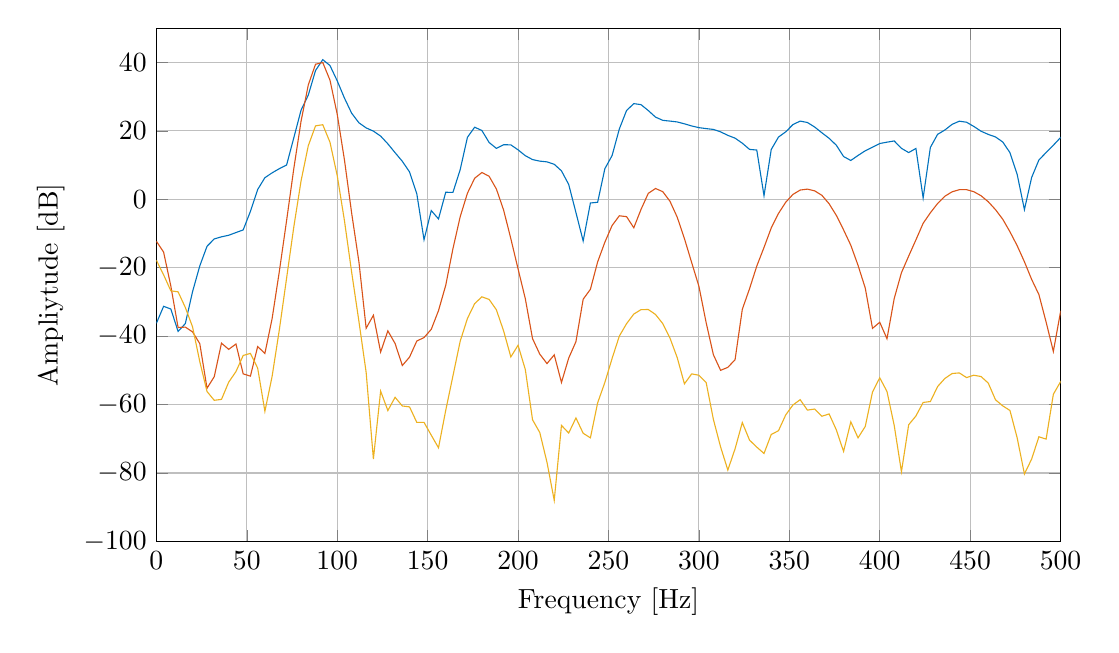
\begin{tikzpicture}

\begin{axis}[%
width=4.521in,
height=2.566in,
at={(0.758in,0.481in)},
scale only axis,
xmin=0,
xmax=500,
xmajorgrids,
ymin=-100,
ymax=50,
ymajorgrids,
xlabel = {Frequency [Hz]},
ylabel = {Ampliytude [dB]},
axis background/.style={fill=white}
]
\addplot [color=mycolor1,solid,forget plot]
  table[row sep=crcr]{%
0	-36.2456627243445\\
4	-31.2759458533165\\
8	-32.0776619775127\\
12	-38.6125202890656\\
16	-36.3345323053453\\
20	-27.0077369967815\\
24	-19.4693943957557\\
28	-13.732339490575\\
32	-11.5807317526438\\
36	-10.9690249691442\\
40	-10.511906993547\\
44	-9.72311303921483\\
48	-8.95211199801677\\
52	-3.53014873376706\\
56	2.84985902328302\\
60	6.32170668333729\\
64	7.73271925463987\\
68	8.95054418483462\\
72	10.0075228410197\\
76	17.9957316464693\\
80	26.045346441109\\
84	30.457626218315\\
88	37.6251571632718\\
92	40.8250217464457\\
96	39.0892035471452\\
100	34.6235828038179\\
104	29.5699447065432\\
108	25.1433887229802\\
112	22.3576097952116\\
116	20.8646916315058\\
120	19.9241336857616\\
124	18.472732341941\\
128	16.204733869856\\
132	13.6196437856485\\
136	11.1013075758865\\
140	7.99166996956162\\
144	1.62396141763164\\
148	-11.8325021373648\\
152	-3.2984151252917\\
156	-5.73668721552419\\
160	2.04711415216091\\
164	2.02985574714828\\
168	8.66924842595592\\
172	18.1109967276352\\
176	21.0704360488716\\
180	20.0996884934558\\
184	16.5965770793381\\
188	14.8930015958921\\
192	15.9524417173127\\
196	15.9057028453994\\
200	14.4547253745259\\
204	12.7449882390982\\
208	11.6056931798645\\
212	11.1535405767167\\
216	10.9390510372725\\
220	10.2310433623445\\
224	8.31476065218885\\
228	4.33545863764797\\
232	-3.87108845717101\\
236	-12.1973708256649\\
240	-1.08169197325651\\
244	-0.874129385856304\\
248	8.94722407260948\\
252	12.7880584999054\\
256	20.5591791800115\\
260	25.9584911846603\\
264	27.9622370372517\\
268	27.6617969197214\\
272	25.9392756536378\\
276	24.0244730781726\\
280	23.0790342884129\\
284	22.8542656462174\\
288	22.6098170894546\\
292	22.0551977243052\\
296	21.4339852432543\\
300	20.9399696925786\\
304	20.6588176126709\\
308	20.4172597744565\\
312	19.7096999527337\\
316	18.684999249698\\
320	17.8721463011533\\
324	16.3924700772466\\
328	14.5866497283843\\
332	14.3917030852375\\
336	1.04546311177496\\
340	14.5530347583429\\
344	18.1829634723254\\
348	19.7136995910232\\
352	21.8401013410047\\
356	22.8547097126057\\
360	22.4468301281197\\
364	21.1285418421379\\
368	19.4431405865107\\
372	17.8213836809138\\
376	15.7977782559822\\
380	12.501619530722\\
384	11.3438865208328\\
388	12.8145580776421\\
392	14.1864434948905\\
396	15.2409846881254\\
400	16.3030994444042\\
404	16.6961658238117\\
408	17.0470470203459\\
412	14.8918980400766\\
416	13.6536675260969\\
420	14.8561014366877\\
424	0.384482173036856\\
428	15.1638958212407\\
432	18.987997947683\\
436	20.245108759595\\
440	21.9016666282161\\
444	22.8265167327497\\
448	22.5224204374786\\
452	21.2931371643563\\
456	19.8996569112845\\
460	18.9651808292316\\
464	18.2280891967941\\
468	16.7551380819249\\
472	13.6385130887548\\
476	7.27369525785863\\
480	-3.01444057081381\\
484	6.38123995057743\\
488	11.4741119860737\\
492	13.6681310178868\\
496	15.8009494496232\\
500	18.0536609546208\\
504	15.3452017404259\\
};
\addplot [color=mycolor2,solid,forget plot]
  table[row sep=crcr]{%
0	-12.2520119318486\\
4	-15.457246347163\\
8	-25.3910173043042\\
12	-37.4725568579776\\
16	-37.3562445654259\\
20	-38.7562873098217\\
24	-42.1876755337237\\
28	-55.2230038989078\\
32	-51.8437687713913\\
36	-42.0532596081128\\
40	-43.8616126543261\\
44	-42.2946076259495\\
48	-51.0209190969441\\
52	-51.6880624037585\\
56	-43.0467675437237\\
60	-45.0414605676052\\
64	-34.8616871742125\\
68	-21.0560951260158\\
72	-6.22477934653492\\
76	9.01920930812603\\
80	22.8214255705148\\
84	33.4224041360244\\
88	39.4694493266955\\
92	39.9787288925826\\
96	34.8176671414911\\
100	24.863578028322\\
104	11.4873261064458\\
108	-4.11512257532409\\
112	-18.3006994856228\\
116	-37.6940669233946\\
120	-33.8883068315645\\
124	-44.6512198998014\\
128	-38.451189683929\\
132	-42.1493579806229\\
136	-48.5844637862039\\
140	-46.1225795980713\\
144	-41.4307693361984\\
148	-40.4105073069862\\
152	-38.0101945947228\\
156	-32.5425091605697\\
160	-25.1447891749562\\
164	-14.4049048926689\\
168	-5.09441327607532\\
172	1.78060576426878\\
176	6.15039756653658\\
180	7.82505796493828\\
184	6.72394606219921\\
188	3.02346566351573\\
192	-3.13070640987898\\
196	-11.5065028162916\\
200	-20.3568425006133\\
204	-29.0366851604597\\
208	-40.7128985278849\\
212	-45.2574360991406\\
216	-48.0175317037803\\
220	-45.4653377556674\\
224	-53.5338028069735\\
228	-46.424098969842\\
232	-41.6150076240414\\
236	-29.2127489596131\\
240	-26.3116395393023\\
244	-18.3124827937642\\
248	-12.5377778555752\\
252	-7.65752118724678\\
256	-4.82030346102452\\
260	-5.07544393128387\\
264	-8.32493945949036\\
268	-2.94762081977006\\
272	1.72178154534596\\
276	3.15551847796161\\
280	2.23430229797106\\
284	-0.579958561067868\\
288	-5.22070801896483\\
292	-11.488501776064\\
296	-18.4977907679757\\
300	-25.4236330689935\\
304	-36.0361296259341\\
308	-45.4229329097162\\
312	-49.9905971669865\\
316	-49.1257655730819\\
320	-46.8804009837873\\
324	-32.1573714025011\\
328	-26.1368574815249\\
332	-19.5256342068777\\
336	-14.0770872227808\\
340	-8.38129953507847\\
344	-4.14466167836757\\
348	-0.872890714687549\\
352	1.42538120503106\\
356	2.70197331240548\\
360	2.9706431978402\\
364	2.46731592419315\\
368	1.16029011129283\\
372	-1.30538261811383\\
376	-4.71639095206136\\
380	-8.94304674713556\\
384	-13.4301118262866\\
388	-19.3087033100694\\
392	-25.9673225742777\\
396	-37.7226046853454\\
400	-35.9447648931512\\
404	-40.7623704428332\\
408	-29.0089260880939\\
412	-21.4586761307658\\
416	-16.5981945929571\\
420	-11.8665589445147\\
424	-7.01866379220067\\
428	-3.94151038515161\\
432	-1.22430450029974\\
436	0.88960531056877\\
440	2.18459573963671\\
444	2.80465667399231\\
448	2.80771957803426\\
452	2.22737220051512\\
456	1.04249713097408\\
460	-0.718753360026654\\
464	-3.02144491943002\\
468	-5.81833646439779\\
472	-9.48808403450077\\
476	-13.5686247049238\\
480	-18.2514089125586\\
484	-23.4257046750688\\
488	-27.8333673151269\\
492	-35.8903151830065\\
496	-44.4761102433801\\
500	-32.8077200235739\\
504	-29.8452907639691\\
};
\addplot [color=mycolor3,solid,forget plot]
  table[row sep=crcr]{%
0	-17.8171623849573\\
4	-22.0871304556474\\
8	-26.7605950757654\\
12	-27.0473590664979\\
16	-31.6140519466276\\
20	-37.2923219172808\\
24	-47.4402911605021\\
28	-56.1895471107498\\
32	-58.7539992284481\\
36	-58.481721686763\\
40	-53.4407053671902\\
44	-50.3639645589143\\
48	-45.653292066664\\
52	-45.033471941546\\
56	-49.3334088914602\\
60	-61.9864928336348\\
64	-51.7396555138723\\
68	-38.0914465652888\\
72	-23.0692349827435\\
76	-8.04622680933582\\
80	5.370575787625\\
84	15.6625081498384\\
88	21.4585352100133\\
92	21.802476278155\\
96	16.6667244284307\\
100	6.92805941959042\\
104	-6.26733413099112\\
108	-21.391851018122\\
112	-35.6899317565\\
116	-50.6197727750267\\
120	-75.9172255179527\\
124	-56.0634402841978\\
128	-61.7508747618951\\
132	-57.8690629310526\\
136	-60.4110604874674\\
140	-60.6839879099036\\
144	-65.2129122668907\\
148	-65.1983597409115\\
152	-68.9547970093869\\
156	-72.6307278963048\\
160	-61.6907453362862\\
164	-51.5850082164483\\
168	-41.4741751381366\\
172	-34.8453736427206\\
176	-30.4916613216851\\
180	-28.5128369135712\\
184	-29.2711115887791\\
188	-32.2887931357218\\
192	-38.4602790192305\\
196	-46.0677094789475\\
200	-42.6696662867624\\
204	-49.7368953446889\\
208	-64.4452938008926\\
212	-68.1605799163304\\
216	-76.8829052489993\\
220	-88.0069185906183\\
224	-66.086657457663\\
228	-68.3191823061978\\
232	-63.9143735805713\\
236	-68.3867782915057\\
240	-69.7241329240411\\
244	-59.5093854684557\\
248	-53.5236219739806\\
252	-46.518637646594\\
256	-39.9835937493057\\
260	-36.3521020561078\\
264	-33.550944148426\\
268	-32.2424634700224\\
272	-32.2207242975908\\
276	-33.6608367553349\\
280	-36.3247560700635\\
284	-40.5601840074546\\
288	-46.2615693544122\\
292	-53.9473997491477\\
296	-51.0308492025798\\
300	-51.4260480650725\\
304	-53.5334880312033\\
308	-64.3125722299687\\
312	-72.3997520936646\\
316	-79.1355686260166\\
320	-72.9352062421103\\
324	-65.2576232966292\\
328	-70.3907922403966\\
332	-72.433258848779\\
336	-74.2918930111868\\
340	-68.7346087080537\\
344	-67.646314097029\\
348	-63.0313832944543\\
352	-60.1149343527707\\
356	-58.573068605131\\
360	-61.6167567025125\\
364	-61.3092912319025\\
368	-63.418442319508\\
372	-62.7361018074775\\
376	-67.3976044937552\\
380	-73.7062659524425\\
384	-65.0437032036963\\
388	-69.7210711588816\\
392	-66.3862663691021\\
396	-56.3221161578425\\
400	-52.1765755690186\\
404	-56.1687953461351\\
408	-66.0958334612276\\
412	-79.6326212226488\\
416	-65.9047091904128\\
420	-63.3360413847449\\
424	-59.3849489318673\\
428	-59.1091138578939\\
432	-54.7217548502314\\
436	-52.3839258562663\\
440	-50.9277593354018\\
444	-50.7464587091174\\
448	-52.111703667707\\
452	-51.42413181944\\
456	-51.8077131156495\\
460	-53.713560851602\\
464	-58.5957179358222\\
468	-60.3717718602905\\
472	-61.719843878435\\
476	-69.7360582460514\\
480	-80.2872255947469\\
484	-75.928207578822\\
488	-69.4186253438429\\
492	-70.0929450696748\\
496	-56.9930897356615\\
500	-53.3123095796073\\
504	-57.5347032563323\\
};
\end{axis}
\end{tikzpicture}%
\caption{The spectrum of accelerometer measurements from time 28.95 - 29.20. The measurements are in ascending order 1, 10, 13, 16 and 19.}
\label{fig:FFT_hit_Main}
\end{figure}

\autoref{fig:FFT_hit_Main} shows that this area is affected by hits on measurement 16 and upwards, refering back to \autoref{subsec:impulses} where it can be seen that an increase in energy level across all frequencies point towards an impulse in the form of a hit. This is particularly seen when comparing measurement 16 through 19. It is possible to see how the fundamental tone at 80 Hz is not increasing dramatically. This is due to the high needs of wattages at this point. However, the entire signals lies more or less 20 dB higher which corresponds to 100 times the energy. This concludes that hits occur but at a very high volume levels \gls{SPL}.

The vibration was also measured on the enclosure but an analysis concludes that the vibration from the enclosure do not change its characteristics at different gains.







%\section{Frequency Response of Measured Data}

In this section the frequency response of the measured data will be analysed to examine if there is any correlation between the frequency responses and the performance of the loudspeaker. From previous section the presented data showed that minimal changes occurred between the datasets. Therefore the expectation is that the frequency response of the measurements will mostly likewise remain almost identical between the datasets. In \autoref{fig:freq_response1} the frequency response of the data measured from the accelerometers and microphone is shown for dataset 1.

\begin{figure}[H]
\centering
\begin{subfigure}[t]{0.37\textwidth}
	\tikzsetnextfilename{FFT_driver1}
	% This file was created by matlab2tikz.
%
%The latest updates can be retrieved from
%  http://www.mathworks.com/matlabcentral/fileexchange/22022-matlab2tikz-matlab2tikz
%where you can also make suggestions and rate matlab2tikz.
%
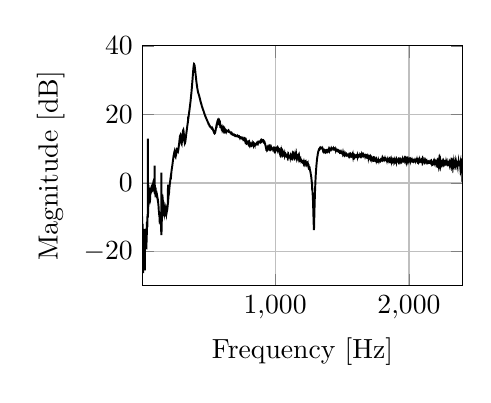
\begin{tikzpicture}

\begin{axis}[%
width=1.6in,
height=1.2in,
at={(1.011in,0.642in)},
scale only axis,
xmin=10,
xmax=2400,
xmajorgrids,
ymin=-30,
ymax=40,
ymajorgrids,
ylabel={Magnitude [dB]},
xlabel={Frequency [Hz]},
axis background/.style={fill=white}
]
\addplot [color=black,solid,line width=0.7pt,forget plot]
  table[row sep=crcr]{%
0	-19.3618707872866\\
0.666675926054529	-35.9021795514571\\
1.33335185210906	-20.4995835912269\\
2.00002777816359	-20.5444223053229\\
2.66670370421811	-9.88468154141047\\
3.33337963027264	-19.4430564977411\\
4.00005555632717	-19.9418145255131\\
4.6667314823817	-11.0447427372739\\
5.33340740843623	-16.0704359338039\\
6.00008333449076	-23.4702797128755\\
6.66675926054529	-15.6619663777543\\
7.33343518659981	-9.76687826406771\\
8.00011111265434	-19.81163092948\\
8.66678703870887	-17.2704521107206\\
9.3334629647634	-14.8299470465014\\
10.0001388908179	-20.9710252598229\\
10.6668148168725	-12.4462531922576\\
11.333490742927	-11.9282433167507\\
12.0001666689815	-20.3262262253202\\
12.666842595036	-19.7394025773231\\
13.3335185210906	-19.6473940807427\\
14.0001944471451	-26.2662831785163\\
14.6668703731996	-14.3734875190756\\
15.3335462992542	-15.6194052031707\\
16.0002222253087	-20.5496811876015\\
16.6668981513632	-22.2090559759572\\
17.3335740774177	-13.975664759218\\
18.0002500034723	-15.7219059175587\\
18.6669259295268	-18.9757168031201\\
19.3336018555813	-20.1126389030472\\
20.0002777816359	-20.0150779499674\\
20.6669537076904	-19.6692319589062\\
21.3336296337449	-20.2893657977048\\
22.0003055597994	-13.5845319182427\\
22.666981485854	-18.3651991731509\\
23.3336574119085	-18.3877906864951\\
24.000333337963	-23.6914867344971\\
24.6670092640176	-13.3952905774092\\
25.3336851900721	-14.8954912714511\\
26.0003611161266	-15.2317825176649\\
26.6670370421811	-14.3703796977619\\
27.3337129682357	-25.5165667215092\\
28.0003888942902	-13.7440540263342\\
28.6670648203447	-17.7645298009446\\
29.3337407463993	-14.7837657270799\\
30.0004166724538	-16.8735833588288\\
30.6670925985083	-17.2615490606666\\
31.3337685245628	-17.5057872025498\\
32.0004444506174	-16.2430944598921\\
32.6671203766719	-16.4407468828219\\
33.3337963027264	-17.3775675554526\\
34.000472228781	-18.1531539923639\\
34.6671481548355	-17.6636361452589\\
35.33382408089	-18.2668892181375\\
36.0005000069445	-19.3154779572481\\
36.6671759329991	-19.0730057493734\\
37.3338518590536	-17.4931961907791\\
38.0005277851081	-18.5459459068643\\
38.6672037111627	-18.5814342471402\\
39.3338796372172	-17.1293154163343\\
40.0005555632717	-17.3384234147972\\
40.6672314893262	-13.1347312756615\\
41.3339074153808	-15.5929452177734\\
42.0005833414353	-14.5776655625952\\
42.6672592674898	-11.4241252846142\\
43.3339351935444	-13.2368355069047\\
44.0006111195989	-12.2062110260313\\
44.6672870456534	-11.3220003063678\\
45.3339629717079	-12.9504502177195\\
46.0006388977625	-9.91595299096013\\
46.667314823817	-9.82517386458058\\
47.3339907498715	-10.1629820842313\\
48.0006666759261	-9.1029695267806\\
48.6673426019806	-9.80998740038481\\
49.3340185280351	-9.97000505908926\\
50.0006944540896	12.9240349727171\\
50.6673703801442	-7.21977883002444\\
51.3340463061987	-7.11446728172143\\
52.0007222322532	-8.97719564464933\\
52.6673981583078	-6.72063400953434\\
53.3340740843623	-6.3749580055128\\
54.0007500104168	-6.90631756701589\\
54.6674259364713	-6.30743722286645\\
55.3341018625259	-5.88202149675894\\
56.0007777885804	-5.61425232039832\\
56.6674537146349	-5.97918208872082\\
57.3341296406895	-5.37794492569941\\
58.000805566744	-4.89271215568237\\
58.6674814927985	-5.17338460687313\\
59.334157418853	-4.98600617637626\\
60.0008333449076	-4.85526946634448\\
60.6675092709621	-5.2761988980378\\
61.3341851970166	-3.78546843623239\\
62.0008611230712	-4.32617760644911\\
62.6675370491257	-4.54211696650046\\
63.3342129751802	-3.88517846686583\\
64.0008889012347	-4.02237599460151\\
64.6675648272893	-3.63286097665071\\
65.3342407533438	-3.87214301509673\\
66.0009166793983	-3.26523646091372\\
66.6675926054529	-3.72316484908041\\
67.3342685315074	-3.0928348687467\\
68.0009444575619	-3.24142211424055\\
68.6676203836164	-2.67465267727076\\
69.334296309671	-3.26876729871548\\
70.0009722357255	-2.63127500896192\\
70.66764816178	-2.51084178131243\\
71.3343240878346	-2.93847776060651\\
72.0010000138891	-2.31819970809246\\
72.6676759399436	-3.02553318854959\\
73.3343518659981	-2.43376505268678\\
74.0010277920527	-2.31815003861385\\
74.6677037181072	-2.31016640184259\\
75.3343796441617	-1.69491841027598\\
76.0010555702163	-2.22955738129066\\
76.6677314962708	-1.72027342301511\\
77.3344074223253	-1.6558429796661\\
78.0010833483798	-1.80714746843256\\
78.6677592744344	-1.81411401941666\\
79.3344352004889	-1.74565457439211\\
80.0011111265434	-1.52549072383373\\
80.667787052598	-1.58400244407407\\
81.3344629786525	-0.794793712460878\\
82.001138904707	-1.21720617302108\\
82.6678148307615	-1.32404377078639\\
83.3344907568161	-1.19859894415666\\
84.0011666828706	-1.54136539234771\\
84.6678426089251	-1.25417213799066\\
85.3345185349797	-1.59876693986671\\
86.0011944610342	-1.39127366917041\\
86.6678703870887	-1.3696455118177\\
87.3345463131432	-1.24349146129673\\
88.0012222391978	-1.32427084946929\\
88.6678981652523	-1.39971551325901\\
89.3345740913068	-1.17434411025682\\
90.0012500173614	-1.21083171739961\\
90.6679259434159	-1.2824931768613\\
91.3346018694704	-1.27007323884887\\
92.0012777955249	-0.966074720727181\\
92.6679537215795	-1.12262786063696\\
93.334629647634	-1.25910159242507\\
94.0013055736885	-1.00924206496683\\
94.667981499743	-1.19814649030848\\
95.3346574257976	-1.03793473306067\\
96.0013333518521	-0.985069630540586\\
96.6680092779066	-1.16576706251535\\
97.3346852039612	-1.13231955371233\\
98.0013611300157	-1.66764064822606\\
98.6680370560702	-1.28672331497108\\
99.3347129821248	-1.3445186725035\\
100.001388908179	5.03925813680822\\
100.668064834234	-1.24492409609696\\
101.334740760288	-1.84894853364229\\
102.001416686343	-1.5057135993022\\
102.668092612397	-1.62581664083084\\
103.334768538452	-1.96026321995936\\
104.001444464506	-1.80858605343605\\
104.668120390561	-1.87696249754052\\
105.334796316616	-1.77338599294492\\
106.00147224267	-1.96371233163815\\
106.668148168725	-2.43242825396346\\
107.334824094779	-1.99629794834388\\
108.001500020834	-2.07333842125666\\
108.668175946888	-2.04693878577049\\
109.334851872943	-2.7856581024142\\
110.001527798997	-2.28962283777454\\
110.668203725052	-2.82932525884246\\
111.334879651106	-2.74366176562584\\
112.001555577161	-2.77203713305229\\
112.668231503215	-2.81106168698214\\
113.33490742927	-3.29193002298192\\
114.001583355324	-2.85516807999158\\
114.668259281379	-3.25622357420913\\
115.334935207433	-2.87083513348013\\
116.001611133488	-3.20098014091963\\
116.668287059542	-3.13931560604944\\
117.334962985597	-3.21800656543537\\
118.001638911652	-3.60361366656882\\
118.668314837706	-4.17266244181744\\
119.334990763761	-3.97386570647672\\
120.001666689815	-4.10317537863612\\
120.66834261587	-4.55642386800676\\
121.335018541924	-4.25647477320912\\
122.001694467979	-4.39406873293558\\
122.668370394033	-4.51138804830031\\
123.335046320088	-4.98742159191303\\
124.001722246142	-5.14486191270147\\
124.668398172197	-4.75589633135072\\
125.335074098251	-5.43127085642699\\
126.001750024306	-5.64842885485132\\
126.66842595036	-5.30074903970846\\
127.335101876415	-6.04512020516773\\
128.001777802469	-6.29132072343327\\
128.668453728524	-6.50695924426763\\
129.335129654579	-6.82140368980889\\
130.001805580633	-7.47075787354341\\
130.668481506688	-7.55572763464663\\
131.335157432742	-8.21634295355302\\
132.001833358797	-8.32120016798544\\
132.668509284851	-8.37506524200766\\
133.335185210906	-8.9496274798399\\
134.00186113696	-9.27578626243634\\
134.668537063015	-8.80783005626224\\
135.335212989069	-9.2782531505472\\
136.001888915124	-9.64742916651176\\
136.668564841178	-9.46825003491031\\
137.335240767233	-10.4050921542696\\
138.001916693287	-11.3250511085103\\
138.668592619342	-11.5516815812687\\
139.335268545396	-11.1106617083089\\
140.001944471451	-11.7499094291161\\
140.668620397506	-10.1510233892866\\
141.33529632356	-11.157217772991\\
142.001972249615	-10.2106984049837\\
142.668648175669	-10.0510334437557\\
143.335324101724	-10.3268554510805\\
144.002000027778	-10.0355459586078\\
144.668675953833	-10.7763809377099\\
145.335351879887	-10.8587694825624\\
146.002027805942	-10.4799795322674\\
146.668703731996	-11.4493056473397\\
147.335379658051	-12.1437142770862\\
148.002055584105	-11.962164877165\\
148.66873151016	-13.5416518045528\\
149.335407436214	-14.1889118439315\\
150.002083362269	3.04128722772059\\
150.668759288323	-15.1869062815816\\
151.335435214378	-13.7380737628693\\
152.002111140433	-14.2196536995097\\
152.668787066487	-13.4046421317761\\
153.335462992542	-11.6471719266991\\
154.002138918596	-10.760690485525\\
154.668814844651	-8.41691304980566\\
155.335490770705	-7.38533557911436\\
156.00216669676	-6.02064320421254\\
156.668842622814	-5.46287813346268\\
157.335518548869	-5.04969251448635\\
158.002194474923	-4.50630124511883\\
158.668870400978	-4.43783654221954\\
159.335546327032	-4.88720353680776\\
160.002222253087	-5.06977429115913\\
160.668898179141	-5.19068972670615\\
161.335574105196	-5.64099493735669\\
162.00225003125	-5.56196878479219\\
162.668925957305	-6.01141409718634\\
163.335601883359	-6.75241892022081\\
164.002277809414	-6.538990401781\\
164.668953735469	-7.23450154339778\\
165.335629661523	-6.74809548714496\\
166.002305587578	-7.05029257720258\\
166.668981513632	-7.39507165753175\\
167.335657439687	-7.48702815002829\\
168.002333365741	-8.58992278330363\\
168.669009291796	-8.52914852452159\\
169.33568521785	-8.6499350226437\\
170.002361143905	-7.8212165466623\\
170.669037069959	-7.89120213363103\\
171.335712996014	-8.07367011944289\\
172.002388922068	-7.87410609432333\\
172.669064848123	-8.17219993186708\\
173.335740774177	-7.76390095527525\\
174.002416700232	-8.28752825751316\\
174.669092626286	-9.02660428520083\\
175.335768552341	-8.49123820860328\\
176.002444478396	-9.17787961327407\\
176.66912040445	-8.95991283252426\\
177.335796330505	-8.76127455026899\\
178.002472256559	-9.04680280690476\\
178.669148182614	-9.00947111443036\\
179.335824108668	-9.31841804953383\\
180.002500034723	-9.27939456248399\\
180.669175960777	-8.71202583157834\\
181.335851886832	-9.50555929637702\\
182.002527812886	-8.65467993330737\\
182.669203738941	-8.62737799434884\\
183.335879664995	-9.25840518347694\\
184.00255559105	-9.04713806452003\\
184.669231517104	-8.5769430502273\\
185.335907443159	-8.67916420279669\\
186.002583369213	-8.26380700268637\\
186.669259295268	-8.42703416133062\\
187.335935221323	-7.99077751566202\\
188.002611147377	-8.43371721076821\\
188.669287073432	-8.37654035264563\\
189.335962999486	-8.22655884060956\\
190.002638925541	-8.24542965380036\\
190.669314851595	-8.29516042022565\\
191.33599077765	-8.26974793241131\\
192.002666703704	-7.82383305400602\\
192.669342629759	-8.08518583158324\\
193.336018555813	-7.94370588210414\\
194.002694481868	-7.93350967469461\\
194.669370407922	-7.70096143221432\\
195.336046333977	-7.50573609828088\\
196.002722260031	-7.29973916755475\\
196.669398186086	-7.03754494912687\\
197.33607411214	-6.85627051694723\\
198.002750038195	-6.35118374603092\\
198.66942596425	-6.27329248670784\\
199.336101890304	-5.62064545943526\\
200.002777816359	-0.520653736743226\\
200.669453742413	-5.75155877791724\\
201.336129668468	-4.4796134774656\\
202.002805594522	-4.72430752959396\\
202.669481520577	-4.45546021526977\\
203.336157446631	-3.75557102781182\\
204.002833372686	-3.8760403407913\\
204.66950929874	-3.58209516706976\\
205.336185224795	-3.07413435211663\\
206.002861150849	-3.40025646658202\\
206.669537076904	-2.69080359845468\\
207.336213002958	-2.45267696602557\\
208.002888929013	-2.27657737542287\\
208.669564855067	-2.00718168263896\\
209.336240781122	-2.04701852008489\\
210.002916707176	-1.69324008482576\\
210.669592633231	-1.37541420512163\\
211.336268559286	-1.13288083349977\\
212.00294448534	-0.978882286512991\\
212.669620411395	-0.702656183358659\\
213.336296337449	-0.417395694808079\\
214.002972263504	-0.0938414326463799\\
214.669648189558	-0.0327216465792262\\
215.336324115613	0.148708855407083\\
216.003000041667	0.353599018349351\\
216.669675967722	0.640722273963735\\
217.336351893776	0.915434231330508\\
218.003027819831	1.08714478615943\\
218.669703745885	1.35820861389876\\
219.33637967194	1.39138473536075\\
220.003055597994	1.58445637848068\\
220.669731524049	1.92489091425733\\
221.336407450103	2.08392184258553\\
222.003083376158	2.29463658656951\\
222.669759302213	2.38872420024993\\
223.336435228267	2.32391680605784\\
224.003111154322	2.75108126293096\\
224.669787080376	2.85452164625662\\
225.336463006431	3.11943011750765\\
226.003138932485	3.25625659268346\\
226.66981485854	3.61479060230108\\
227.336490784594	3.78807072357767\\
228.003166710649	3.95529919063432\\
228.669842636703	4.16890859721735\\
229.336518562758	4.27608573371528\\
230.003194488812	4.45094403532182\\
230.669870414867	4.75972997884267\\
231.336546340921	4.81041865641967\\
232.003222266976	5.01992162693982\\
232.66989819303	5.1368566929275\\
233.336574119085	5.37977685110137\\
234.00325004514	5.57911241316725\\
234.669925971194	5.886281344509\\
235.336601897249	5.95716756450319\\
236.003277823303	6.24665076575757\\
236.669953749358	6.48035740261547\\
237.336629675412	6.59231804135953\\
238.003305601467	6.7595849546891\\
238.669981527521	6.96399230087505\\
239.336657453576	7.18840104598157\\
240.00333337963	7.34042905452338\\
240.670009305685	7.52067395403219\\
241.336685231739	7.78622676943283\\
242.003361157794	7.92212176337835\\
242.670037083848	8.02632475838035\\
243.336713009903	8.24755980034838\\
244.003388935957	8.31487755452782\\
244.670064862012	8.470129661696\\
245.336740788066	8.54651053668772\\
246.003416714121	8.66806739733013\\
246.670092640176	8.83423476835627\\
247.33676856623	8.86612833832024\\
248.003444492285	9.07134124641547\\
248.670120418339	9.19343952631\\
249.336796344394	9.23323500853091\\
250.003472270448	9.32917023555425\\
250.670148196503	9.22395032652007\\
251.336824122557	9.13451808256684\\
252.003500048612	9.08731067564757\\
252.670175974666	8.79771825972886\\
253.336851900721	8.47691499356256\\
254.003527826775	8.19265450674294\\
254.67020375283	8.11053299755807\\
255.336879678884	7.8776402441604\\
256.003555604939	7.79160855896555\\
256.670231530993	7.83822328837478\\
257.336907457048	7.76763923640498\\
258.003583383103	7.91120444175719\\
258.670259309157	7.91612951645949\\
259.336935235212	8.06824101762504\\
260.003611161266	8.07494836406927\\
260.670287087321	8.23213331881161\\
261.336963013375	8.35977759477462\\
262.00363893943	8.62660813340609\\
262.670314865484	8.76475356215733\\
263.336990791539	9.00975952747425\\
264.003666717593	9.2256387347976\\
264.670342643648	9.41713264155132\\
265.337018569702	9.59861537432747\\
266.003694495757	9.55659118309994\\
266.670370421811	9.69957805668921\\
267.337046347866	9.66825541135089\\
268.00372227392	9.79519246191875\\
268.670398199975	9.80416559193101\\
269.33707412603	9.82703383043057\\
270.003750052084	9.68425574584365\\
270.670425978139	9.55682305741921\\
271.337101904193	9.41527968725362\\
272.003777830248	9.35609483611069\\
272.670453756302	9.24650902633177\\
273.337129682357	9.21320342348463\\
274.003805608411	9.20658559249051\\
274.670481534466	9.1675925688572\\
275.33715746052	9.30950450253818\\
276.003833386575	9.40606610828403\\
276.670509312629	9.57354347722375\\
277.337185238684	9.65703031885105\\
278.003861164738	9.96843184510568\\
278.670537090793	10.109811346222\\
279.337213016847	10.2745766901816\\
280.003888942902	10.493837169901\\
280.670564868956	10.7057934412898\\
281.337240795011	10.9513089721492\\
282.003916721066	11.1196552776977\\
282.67059264712	11.3770962150196\\
283.337268573175	11.5223683607698\\
284.003944499229	11.7237586181509\\
284.670620425284	12.0345613251209\\
285.337296351338	12.2703988487711\\
286.003972277393	12.5279272205309\\
286.670648203447	12.7416227815932\\
287.337324129502	12.9073142387462\\
288.004000055556	13.1180975787029\\
288.670675981611	13.333831397237\\
289.337351907665	13.5670474406913\\
290.00402783372	13.6373832842423\\
290.670703759774	13.7336113664837\\
291.337379685829	13.8146802869948\\
292.004055611883	13.8867266611167\\
292.670731537938	13.9426041891924\\
293.337407463993	13.7950036884169\\
294.004083390047	13.7070665226796\\
294.670759316102	13.5445840514981\\
295.337435242156	13.308689775809\\
296.004111168211	13.0440508478036\\
296.670787094265	12.7680920257627\\
297.33746302032	12.4142136041678\\
298.004138946374	12.2450852754287\\
298.670814872429	11.9564549319363\\
299.337490798483	11.6258386404829\\
300.004166724538	12.2684439114719\\
300.670842650592	11.6229937666425\\
301.337518576647	11.4374183909306\\
302.004194502701	11.3813821254475\\
302.670870428756	11.6490669280708\\
303.33754635481	11.8056923728049\\
304.004222280865	11.9167095181664\\
304.67089820692	12.1013743018492\\
305.337574132974	12.4757414084964\\
306.004250059029	12.6877860532945\\
306.670925985083	12.9221839479462\\
307.337601911138	13.2515852007202\\
308.004277837192	13.6256753511003\\
308.670953763247	13.7629636930123\\
309.337629689301	14.0857124478674\\
310.004305615356	14.4385359063525\\
310.67098154141	14.6574312831774\\
311.337657467465	14.7989979451058\\
312.004333393519	15.1433103039367\\
312.671009319574	15.300451077485\\
313.337685245628	15.3596258012415\\
314.004361171683	15.4610068622099\\
314.671037097737	15.5093536938561\\
315.337713023792	15.3241037375253\\
316.004388949847	15.1987447944542\\
316.671064875901	15.0418771577208\\
317.337740801956	14.705894533561\\
318.00441672801	14.4189846794481\\
318.671092654065	14.071762199169\\
319.337768580119	13.6736985288621\\
320.004444506174	13.3741171124124\\
320.671120432228	13.1263467212002\\
321.337796358283	12.7215684804356\\
322.004472284337	12.4631415681196\\
322.671148210392	12.2463477055507\\
323.337824136446	12.0011302606234\\
324.004500062501	11.8984163784686\\
324.671175988555	11.7539313190426\\
325.33785191461	11.6269151414737\\
326.004527840664	11.7039112439033\\
326.671203766719	11.6990518883027\\
327.337879692774	11.6892884983601\\
328.004555618828	11.8944320306926\\
328.671231544883	11.9053719841116\\
329.337907470937	12.0472273530908\\
330.004583396992	12.2509789817655\\
330.671259323046	12.3680599176696\\
331.337935249101	12.638658943634\\
332.004611175155	12.7793608680765\\
332.67128710121	13.0093969748005\\
333.337963027264	13.2479431438629\\
334.004638953319	13.3902878141347\\
334.671314879373	13.6414326564039\\
335.337990805428	13.8752340445966\\
336.004666731482	14.072334978583\\
336.671342657537	14.3178892978025\\
337.338018583591	14.4548758441018\\
338.004694509646	14.7313876890009\\
338.671370435701	14.895318907374\\
339.338046361755	15.0835656030104\\
340.00472228781	15.3484762287606\\
340.671398213864	15.4749435079211\\
341.338074139919	15.7885587498514\\
342.004750065973	15.8653297787316\\
342.671425992028	16.1692239080047\\
343.338101918082	16.3364392416717\\
344.004777844137	16.5375356826601\\
344.671453770191	16.7465089878244\\
345.338129696246	16.8689924903991\\
346.0048056223	17.1428477313714\\
346.671481548355	17.2224447025625\\
347.338157474409	17.5285110516813\\
348.004833400464	17.6448279591173\\
348.671509326518	17.8805075734288\\
349.338185252573	18.0337037472689\\
350.004861178627	18.4750360674794\\
350.671537104682	18.4271588641798\\
351.338213030737	18.6396716938208\\
352.004888956791	18.817678443432\\
352.671564882846	19.0002002370105\\
353.3382408089	19.2145298232811\\
354.004916734955	19.3697422309362\\
354.671592661009	19.650137471914\\
355.338268587064	19.773616656178\\
356.004944513118	20.0281417507844\\
356.671620439173	20.1588654093105\\
357.338296365227	20.4255123616847\\
358.004972291282	20.5303176375592\\
358.671648217336	20.7990100777883\\
359.338324143391	20.9091847448413\\
360.005000069445	21.2009998211123\\
360.6716759955	21.3288520965485\\
361.338351921554	21.5974520900444\\
362.005027847609	21.7406101663951\\
362.671703773664	22.0036786609798\\
363.338379699718	22.1758939389062\\
364.005055625773	22.4092065617165\\
364.671731551827	22.6043360131825\\
365.338407477882	22.8145214531445\\
366.005083403936	23.0617249493562\\
366.671759329991	23.2383753963735\\
367.338435256045	23.5017511838225\\
368.0051111821	23.6618519776456\\
368.671787108154	23.977567524018\\
369.338463034209	24.1377164918625\\
370.005138960263	24.4722243451756\\
370.671814886318	24.6391151153694\\
371.338490812372	24.9651881333226\\
372.005166738427	25.1941275253484\\
372.671842664481	25.4573765925804\\
373.338518590536	25.7351898199429\\
374.005194516591	25.9486361440607\\
374.671870442645	26.2832248300519\\
375.3385463687	26.4693507438062\\
376.005222294754	26.8144423497695\\
376.671898220809	27.0407559976594\\
377.338574146863	27.3701293895772\\
378.005250072918	27.680314120169\\
378.671925998972	27.9504246390054\\
379.338601925027	28.3454701276926\\
380.005277851081	28.5897427933487\\
380.671953777136	28.9598274560529\\
381.33862970319	29.2536896482888\\
382.005305629245	29.5453436058301\\
382.671981555299	29.9355965603662\\
383.338657481354	30.1901741693537\\
384.005333407408	30.6024607334653\\
384.672009333463	30.9408032580226\\
385.338685259517	31.2464303425154\\
386.005361185572	31.6582574166453\\
386.672037111627	31.9166682784181\\
387.338713037681	32.274553603347\\
388.005388963736	32.6352470836804\\
388.67206488979	32.8866022402636\\
389.338740815845	33.274612379558\\
390.005416741899	33.5224629896123\\
390.672092667954	33.7326211728478\\
391.338768594008	34.0294594929755\\
392.005444520063	34.1528217813387\\
392.672120446117	34.3275564638173\\
393.338796372172	34.4921494668572\\
394.005472298226	34.4524799900155\\
394.672148224281	34.5059415132715\\
395.338824150335	34.5379844686153\\
396.00550007639	34.4529508200051\\
396.672176002444	34.4829120732413\\
397.338851928499	34.4345855545715\\
398.005527854554	34.27809377157\\
398.672203780608	34.2568437771917\\
399.338879706663	34.150150332169\\
400.005555632717	33.8825667999354\\
400.672231558772	33.7079545246617\\
401.338907484826	33.5456191717806\\
402.005583410881	33.2569646041632\\
402.672259336935	33.0118281021832\\
403.33893526299	32.8101399600196\\
404.005611189044	32.5135652481275\\
404.672287115099	32.2724666422037\\
405.338963041153	32.0603665146494\\
406.005638967208	31.7709155855659\\
406.672314893262	31.5044802920053\\
407.338990819317	31.3132797832042\\
408.005666745371	31.065515456776\\
408.672342671426	30.7580187562882\\
409.339018597481	30.5580858508745\\
410.005694523535	30.3814806356686\\
410.67237044959	30.0840019715765\\
411.339046375644	29.8351961702988\\
412.005722301699	29.7017199577745\\
412.672398227753	29.4682927059066\\
413.339074153808	29.194237507581\\
414.005750079862	29.0338915668757\\
414.672426005917	28.8537213867012\\
415.339101931971	28.6409556880654\\
416.005777858026	28.4209807945455\\
416.67245378408	28.2303070369924\\
417.339129710135	28.10569740321\\
418.005805636189	27.9013742615739\\
418.672481562244	27.6773246424915\\
419.339157488298	27.5411580665293\\
420.005833414353	27.4461017056009\\
420.672509340407	27.2479285245684\\
421.339185266462	27.0386024971026\\
422.005861192517	26.9571503298195\\
422.672537118571	26.8396501979411\\
423.339213044626	26.7515608658471\\
424.00588897068	26.5615335036433\\
424.672564896735	26.4335183800764\\
425.339240822789	26.3898871635666\\
426.005916748844	26.3303199681989\\
426.672592674898	26.1673378111597\\
427.339268600953	26.0862711715932\\
428.005944527007	25.9948121779699\\
428.672620453062	25.9758807816233\\
429.339296379116	25.8911701560308\\
430.005972305171	25.7621120146669\\
430.672648231225	25.6623947562977\\
431.33932415728	25.5856764220714\\
432.006000083334	25.5443756100151\\
432.672676009389	25.4873050488812\\
433.339351935444	25.3240776275726\\
434.006027861498	25.2329882518413\\
434.672703787553	25.0844787960022\\
435.339379713607	25.073088832736\\
436.006055639662	24.9697441411312\\
436.672731565716	24.8721485403557\\
437.339407491771	24.7170291418084\\
438.006083417825	24.5580523600165\\
438.67275934388	24.4958749979621\\
439.339435269934	24.3796001834163\\
440.006111195989	24.3511004999882\\
440.672787122043	24.1954836461562\\
441.339463048098	24.0752971763901\\
442.006138974152	23.9383321411095\\
442.672814900207	23.8441399968708\\
443.339490826261	23.7755733812962\\
444.006166752316	23.7002205221968\\
444.672842678371	23.6007989924081\\
445.339518604425	23.5099756219178\\
446.00619453048	23.3793801644176\\
446.672870456534	23.2498904206607\\
447.339546382589	23.1675170539806\\
448.006222308643	23.0814009437549\\
448.672898234698	23.0116942793781\\
449.339574160752	22.964840851347\\
450.006250086807	22.9458704611028\\
450.672926012861	22.7783538254155\\
451.339601938916	22.6382110135418\\
452.00627786497	22.5476970468293\\
452.672953791025	22.4317637900438\\
453.339629717079	22.3681217755119\\
454.006305643134	22.2761764703997\\
454.672981569188	22.2294736097782\\
455.339657495243	22.1449451202068\\
456.006333421298	22.1160098296591\\
456.673009347352	22.0060886937568\\
457.339685273407	21.9304768469233\\
458.006361199461	21.8244093856888\\
458.673037125516	21.7316223491682\\
459.33971305157	21.6257007503832\\
460.006388977625	21.5309560014764\\
460.673064903679	21.4782096457126\\
461.339740829734	21.4014578573023\\
462.006416755788	21.3592599180213\\
462.673092681843	21.256840338377\\
463.339768607897	21.2065775637823\\
464.006444533952	21.1350130881169\\
464.673120460006	21.0839212617895\\
465.339796386061	21.0055807317284\\
466.006472312115	20.9206656945536\\
466.67314823817	20.8391310697489\\
467.339824164225	20.7488575893734\\
468.006500090279	20.6839066870886\\
468.673176016334	20.6176278655441\\
469.339851942388	20.515563407399\\
470.006527868443	20.4489964588962\\
470.673203794497	20.3415372715676\\
471.339879720552	20.2434423446577\\
472.006555646606	20.2238547972236\\
472.673231572661	20.1500104700638\\
473.339907498715	20.0641149313031\\
474.00658342477	20.0155520841237\\
474.673259350824	19.8984088787438\\
475.339935276879	19.8167830452497\\
476.006611202933	19.7829865189436\\
476.673287128988	19.6697896991569\\
477.339963055042	19.5995051883076\\
478.006638981097	19.5952348274665\\
478.673314907152	19.5014798057631\\
479.339990833206	19.4176958625874\\
480.006666759261	19.3725855091289\\
480.673342685315	19.2757692541619\\
481.34001861137	19.2196493243922\\
482.006694537424	19.2042050143783\\
482.673370463479	19.0951235276728\\
483.340046389533	19.0102230895272\\
484.006722315588	18.9773397078674\\
484.673398241642	18.9312526849428\\
485.340074167697	18.8557475227714\\
486.006750093751	18.7949903251266\\
486.673426019806	18.7466929988789\\
487.34010194586	18.690511732119\\
488.006777871915	18.6189838500254\\
488.673453797969	18.5860954078857\\
489.340129724024	18.5331296321922\\
490.006805650078	18.4579266990112\\
490.673481576133	18.372315235375\\
491.340157502188	18.3319678573866\\
492.006833428242	18.2823146786698\\
492.673509354297	18.1736580621393\\
493.340185280351	18.1154465819649\\
494.006861206406	18.0874254414673\\
494.67353713246	17.9971101242718\\
495.340213058515	17.9153642911631\\
496.006888984569	17.8558607499057\\
496.673564910624	17.8272089195585\\
497.340240836678	17.7689684682805\\
498.006916762733	17.7240616823976\\
498.673592688787	17.6788090881146\\
499.340268614842	17.6161004207237\\
500.006944540896	17.5310425513652\\
500.673620466951	17.4425271469796\\
501.340296393005	17.3418460395877\\
502.00697231906	17.2758221677175\\
502.673648245115	17.267028255022\\
503.340324171169	17.2781276668744\\
504.007000097224	17.210917417503\\
504.673676023278	17.1200646646595\\
505.340351949333	17.1059976868596\\
506.007027875387	17.1007664238695\\
506.673703801442	17.0331785872377\\
507.340379727496	16.9913466987233\\
508.007055653551	16.8890069270035\\
508.673731579605	16.7891066779324\\
509.34040750566	16.7300467123014\\
510.007083431714	16.7381196955819\\
510.673759357769	16.7328369246324\\
511.340435283823	16.7169103707291\\
512.007111209878	16.6382801236244\\
512.673787135932	16.547096015275\\
513.340463061987	16.4854386771388\\
514.007138988041	16.4542937923094\\
514.673814914096	16.4454673311036\\
515.340490840151	16.4489332837606\\
516.007166766205	16.4147961994688\\
516.67384269226	16.3885516307465\\
517.340518618314	16.2706279815487\\
518.007194544369	16.2591221149596\\
518.673870470423	16.233324992577\\
519.340546396478	16.244104383152\\
520.007222322532	16.2195029701752\\
520.673898248587	16.1556079743307\\
521.340574174641	16.1440169406125\\
522.007250100696	16.1674559478337\\
522.67392602675	16.1547922202727\\
523.340601952805	16.1554122758746\\
524.007277878859	16.152751152871\\
524.673953804914	16.1225027133183\\
525.340629730968	16.0499008571852\\
526.007305657023	16.0795852066358\\
526.673981583078	16.1017003009515\\
527.340657509132	16.0856263004078\\
528.007333435187	16.0056037949166\\
528.674009361241	15.9978384794813\\
529.340685287296	15.9499654219996\\
530.00736121335	16.003658067844\\
530.674037139405	15.9471291338518\\
531.340713065459	15.8773895206512\\
532.007388991514	15.8553531599656\\
532.674064917568	15.8745775444435\\
533.340740843623	15.8172777924018\\
534.007416769677	15.751167853204\\
534.674092695732	15.647045896088\\
535.340768621786	15.6247740794223\\
536.007444547841	15.582567223678\\
536.674120473896	15.4662287045036\\
537.34079639995	15.3955257377633\\
538.007472326005	15.3540519147725\\
538.674148252059	15.3184859454046\\
539.340824178114	15.2142494108425\\
540.007500104168	15.0955185860154\\
540.674176030223	15.062525615901\\
541.340851956277	15.0007524619735\\
542.007527882332	14.9025895827768\\
542.674203808386	14.8018046876672\\
543.340879734441	14.7850196988538\\
544.007555660495	14.7340519595461\\
544.67423158655	14.6269471808843\\
545.340907512604	14.6217859780869\\
546.007583438659	14.5934141185214\\
546.674259364713	14.534385789673\\
547.340935290768	14.4938739308286\\
548.007611216823	14.5311076929047\\
548.674287142877	14.5753219172441\\
549.340963068932	14.4832816844596\\
550.007638994986	14.5024924292087\\
550.674314921041	14.6453692764469\\
551.340990847095	14.6303311481102\\
552.00766677315	14.7006516644172\\
552.674342699204	14.8781835538091\\
553.341018625259	14.8764908876774\\
554.007694551313	14.995040459506\\
554.674370477368	15.1276311512138\\
555.341046403422	15.2651930513634\\
556.007722329477	15.4016446287971\\
556.674398255531	15.5902671350371\\
557.341074181586	15.7385518181621\\
558.00775010764	15.8431428971125\\
558.674426033695	16.0986336876973\\
559.341101959749	16.2007778182753\\
560.007777885804	16.2836797149855\\
560.674453811858	16.5437508861976\\
561.341129737913	16.5899679771811\\
562.007805663968	16.7156325267429\\
562.674481590022	16.9194361753216\\
563.341157516077	16.9085567183153\\
564.007833442131	17.1211072544243\\
564.674509368186	17.1512557343425\\
565.34118529424	17.0857459059384\\
566.007861220295	17.3069040450994\\
566.674537146349	17.4528274790765\\
567.341213072404	17.5256146547363\\
568.007888998458	17.6918720512982\\
568.674564924513	17.6703158465671\\
569.341240850567	17.7938311019778\\
570.007916776622	17.8906645467607\\
570.674592702676	17.826349172351\\
571.341268628731	17.9664138185063\\
572.007944554785	17.966508251008\\
572.67462048084	17.9574442607058\\
573.341296406895	18.0296151345562\\
574.007972332949	17.999888482376\\
574.674648259004	18.106721858489\\
575.341324185058	18.059163234698\\
576.008000111113	18.0474279390616\\
576.674676037167	18.0904361152733\\
577.341351963222	17.9682624220956\\
578.008027889276	18.0611991994242\\
578.674703815331	17.9689211591393\\
579.341379741385	17.9958547488359\\
580.00805566744	17.9259833215245\\
580.674731593494	17.8496803933777\\
581.341407519549	17.9143362018226\\
582.008083445603	17.7492996791415\\
582.674759371658	17.8030287711394\\
583.341435297712	17.6432104530114\\
584.008111223767	17.6781893434403\\
584.674787149822	17.5529599100494\\
585.341463075876	17.5158046063981\\
586.008139001931	17.5143171799659\\
586.674814927985	17.358332057589\\
587.34149085404	17.3509933314181\\
588.008166780094	17.1707471744715\\
588.674842706149	17.2378131402912\\
589.341518632203	17.0291383177995\\
590.008194558258	17.0820169695886\\
590.674870484312	16.8696166053489\\
591.341546410367	16.8689438635772\\
592.008222336421	16.6909351796721\\
592.674898262476	16.7283398771291\\
593.34157418853	16.6093793369855\\
594.008250114585	16.5725131254014\\
594.674926040639	16.489629826362\\
595.341601966694	16.4613662983083\\
596.008277892749	16.3360261545365\\
596.674953818803	16.2886794174475\\
597.341629744858	16.2324550134901\\
598.008305670912	16.1744263898047\\
598.674981596967	16.079717588956\\
599.341657523021	16.1259435635265\\
600.008333449076	15.9767148955137\\
600.67500937513	16.0139479376889\\
601.341685301185	15.9254718077809\\
602.008361227239	15.9435933343133\\
602.675037153294	15.8624794178313\\
603.341713079348	15.906156928152\\
604.008389005403	15.7747610080793\\
604.675064931457	15.8888550080739\\
605.341740857512	15.761247222628\\
606.008416783566	15.8165923481738\\
606.675092709621	15.7496528386067\\
607.341768635676	15.7508714646688\\
608.00844456173	15.6857656912273\\
608.675120487785	15.7167625244519\\
609.341796413839	15.6995488269068\\
610.008472339894	15.6424265324421\\
610.675148265948	15.6646889860933\\
611.341824192003	15.5981063503046\\
612.008500118057	15.6954236013886\\
612.675176044112	15.5575633767151\\
613.341851970166	15.6133037649105\\
614.008527896221	15.5459740740405\\
614.675203822275	15.5504160664722\\
615.34187974833	15.5655742560186\\
616.008555674384	15.4618995923198\\
616.675231600439	15.5687384925729\\
617.341907526493	15.4737390839156\\
618.008583452548	15.5199889963706\\
618.675259378603	15.4965481480473\\
619.341935304657	15.4710211904958\\
620.008611230711	15.50636608978\\
620.675287156766	15.3896184829142\\
621.341963082821	15.4296222622508\\
622.008639008875	15.406192517108\\
622.67531493493	15.3170342522488\\
623.341990860984	15.4162122020578\\
624.008666787039	15.2830087759572\\
624.675342713093	15.2979620938838\\
625.342018639148	15.3215521484245\\
626.008694565202	15.2020027546952\\
626.675370491257	15.2603739246503\\
627.342046417311	15.1819334534858\\
628.008722343366	15.1829092050369\\
628.67539826942	15.2310981588317\\
629.342074195475	15.1424132219261\\
630.008750121529	15.1299404551401\\
630.675426047584	15.1044124484591\\
631.342101973638	15.0384233724096\\
632.008777899693	15.0628907154921\\
632.675453825748	15.0643895175643\\
633.342129751802	14.991755602926\\
634.008805677857	15.0289376836571\\
634.675481603911	14.9567612139926\\
635.342157529966	15.0404620075365\\
636.00883345602	15.0039848712989\\
636.675509382075	15.0038177581841\\
637.342185308129	15.0024032748583\\
638.008861234184	15.05293545392\\
638.675537160238	14.9832680858656\\
639.342213086293	14.9901300836212\\
640.008889012347	15.0591159996423\\
640.675564938402	15.044859025629\\
641.342240864456	15.083351266305\\
642.008916790511	15.1263758033044\\
642.675592716565	15.1028332768199\\
643.34226864262	15.1055323300386\\
644.008944568675	15.1209244741918\\
644.675620494729	15.1658218038784\\
645.342296420784	15.1515474544963\\
646.008972346838	15.1795048076326\\
646.675648272893	15.1905055639529\\
647.342324198947	15.1396839278998\\
648.009000125002	15.1375807670928\\
648.675676051056	15.178874057423\\
649.342351977111	15.2010996414745\\
650.009027903165	15.1899210122617\\
650.67570382922	15.1515109708583\\
651.342379755274	15.195063979341\\
652.009055681329	15.1197695293232\\
652.675731607383	15.1109590932212\\
653.342407533438	15.1430706776879\\
654.009083459492	15.060146027094\\
654.675759385547	15.0397822060428\\
655.342435311602	15.0136621212574\\
656.009111237656	15.0264153167971\\
656.675787163711	15.0010667411867\\
657.342463089765	14.9359942129756\\
658.00913901582	14.9456725312995\\
658.675814941874	14.937564205371\\
659.342490867929	14.9330347757354\\
660.009166793983	14.8476593767594\\
660.675842720038	14.8298010178927\\
661.342518646092	14.8521411911059\\
662.009194572147	14.8138021405902\\
662.675870498201	14.7799592033147\\
663.342546424256	14.7602882786645\\
664.00922235031	14.7843995700771\\
664.675898276365	14.7613031185636\\
665.342574202419	14.6997739103442\\
666.009250128474	14.647849207414\\
666.675926054529	14.6741076767612\\
667.342601980583	14.658983418656\\
668.009277906638	14.6340029278413\\
668.675953832692	14.5802675738556\\
669.342629758747	14.5500436678723\\
670.009305684801	14.526178486487\\
670.675981610856	14.5394770773497\\
671.34265753691	14.5219385320991\\
672.009333462965	14.4986132756945\\
672.676009389019	14.4352178124029\\
673.342685315074	14.4485954476707\\
674.009361241128	14.4878402138349\\
674.676037167183	14.4013804107998\\
675.342713093237	14.4192010349633\\
676.009389019292	14.3625027237386\\
676.676064945346	14.343631158623\\
677.342740871401	14.3402153760337\\
678.009416797456	14.3082554796504\\
678.67609272351	14.3442732888289\\
679.342768649565	14.2861876061887\\
680.009444575619	14.2689792423788\\
680.676120501674	14.2123174718637\\
681.342796427728	14.2336900519799\\
682.009472353783	14.238650398911\\
682.676148279837	14.2133455917976\\
683.342824205892	14.2244965388138\\
684.009500131946	14.1629816041953\\
684.676176058001	14.1302589440397\\
685.342851984055	14.1066697218618\\
686.00952791011	14.1357085205693\\
686.676203836164	14.102929134461\\
687.342879762219	14.1359172429107\\
688.009555688273	14.1156655571112\\
688.676231614328	14.0913762570809\\
689.342907540382	14.029543568363\\
690.009583466437	14.0179752259669\\
690.676259392492	14.0016672403027\\
691.342935318546	14.0045088610928\\
692.009611244601	14.0253395338315\\
692.676287170655	13.9844126382275\\
693.34296309671	13.9683046235232\\
694.009639022764	13.985898212397\\
694.676314948819	13.9584388282645\\
695.342990874873	13.9291291440968\\
696.009666800928	13.958451935271\\
696.676342726982	13.921909930188\\
697.343018653037	13.8815257231815\\
698.009694579091	13.8551671378551\\
698.676370505146	13.8318432190888\\
699.3430464312	13.8788000375133\\
700.009722357255	13.8386692913296\\
700.676398283309	13.8642243706605\\
701.343074209364	13.8919960314968\\
702.009750135419	13.8970949708776\\
702.676426061473	13.908649011525\\
703.343101987528	13.867472690205\\
704.009777913582	13.8472921888497\\
704.676453839637	13.8153997187105\\
705.343129765691	13.8194229330283\\
706.009805691746	13.8193839467886\\
706.6764816178	13.7576744413756\\
707.343157543855	13.7281335630431\\
708.009833469909	13.7581090389923\\
708.676509395964	13.7336444513536\\
709.343185322018	13.7368958052653\\
710.009861248073	13.7404630204994\\
710.676537174127	13.720487741455\\
711.343213100182	13.7038925605696\\
712.009889026236	13.7181577154569\\
712.676564952291	13.7335300093784\\
713.343240878346	13.7577661581475\\
714.0099168044	13.7601406807116\\
714.676592730455	13.7366848146595\\
715.343268656509	13.7165988254693\\
716.009944582564	13.7062605715623\\
716.676620508618	13.7301886799278\\
717.343296434673	13.6846240935792\\
718.009972360727	13.6841924107272\\
718.676648286782	13.7175729878836\\
719.343324212836	13.6415952930352\\
720.010000138891	13.6483893505625\\
720.676676064945	13.6483449021777\\
721.343351991	13.6215366069217\\
722.010027917054	13.6291236851842\\
722.676703843109	13.654633097726\\
723.343379769163	13.6096098008079\\
724.010055695218	13.5721151672515\\
724.676731621273	13.5858637068171\\
725.343407547327	13.5478677057616\\
726.010083473382	13.5696625277931\\
726.676759399436	13.5325465036717\\
727.343435325491	13.5615185372619\\
728.010111251545	13.5466849020637\\
728.6767871776	13.5685429756374\\
729.343463103654	13.5786128955822\\
730.010139029709	13.5405076255293\\
730.676814955763	13.5675248733976\\
731.343490881818	13.5860519296907\\
732.010166807872	13.5335257802545\\
732.676842733927	13.4821114190032\\
733.343518659981	13.4454154861402\\
734.010194586036	13.3868015219426\\
734.67687051209	13.3644298004664\\
735.343546438145	13.3412333772738\\
736.0102223642	13.3290768855355\\
736.676898290254	13.259861063814\\
737.343574216309	13.3489657320765\\
738.010250142363	13.3250303096578\\
738.676926068418	13.346910397895\\
739.343601994472	13.3460464182725\\
740.010277920527	13.3451647607941\\
740.676953846581	13.2743684872826\\
741.343629772636	13.2017987113616\\
742.01030569869	13.1174332027916\\
742.676981624745	13.1181665794177\\
743.343657550799	13.1619966972896\\
744.010333476854	13.2088612653572\\
744.677009402908	13.1827927301895\\
745.343685328963	13.1677012226232\\
746.010361255017	13.1204129038755\\
746.677037181072	13.1066997017076\\
747.343713107127	13.0779342325855\\
748.010389033181	13.027765696596\\
748.677064959236	13.0200117247697\\
749.34374088529	13.0515695854367\\
750.010416811345	13.1011932069225\\
750.677092737399	13.0765327786098\\
751.343768663454	13.062743954509\\
752.010444589508	13.0234907363263\\
752.677120515563	12.915229297473\\
753.343796441617	12.9078552517946\\
754.010472367672	12.9750077786914\\
754.677148293726	13.0475255385649\\
755.343824219781	13.0111054356309\\
756.010500145835	12.8967808868795\\
756.67717607189	12.8722488677805\\
757.343851997944	12.8999443995808\\
758.010527923999	12.9678212910269\\
758.677203850054	12.9341222028267\\
759.343879776108	12.8952145884744\\
760.010555702162	12.8800271318284\\
760.677231628217	12.8433816295036\\
761.343907554272	12.7688938392208\\
762.010583480326	12.817057567726\\
762.677259406381	12.8813228497882\\
763.343935332435	12.8321431531282\\
764.01061125849	12.7035393455459\\
764.677287184544	12.6933336234692\\
765.343963110599	12.7937769525569\\
766.010639036653	12.7880499823581\\
766.677314962708	12.6795334340502\\
767.343990888762	12.6250611543289\\
768.010666814817	12.6365425805558\\
768.677342740871	12.6812556725178\\
769.344018666926	12.5955510900948\\
770.01069459298	12.6065046038311\\
770.677370519035	12.5694564576013\\
771.344046445089	12.5221791126319\\
772.010722371144	12.6278537968144\\
772.677398297199	12.5634413797002\\
773.344074223253	12.4161992845673\\
774.010750149308	12.4064247671703\\
774.677426075362	12.4937433663734\\
775.344102001417	12.4249752297075\\
776.010777927471	12.3158613673551\\
776.677453853526	12.3873756957646\\
777.34412977958	12.3607734372351\\
778.010805705635	12.2584696901824\\
778.677481631689	12.2077551447013\\
779.344157557744	12.2149410397764\\
780.010833483798	12.3003354874215\\
780.677509409853	12.1666724230239\\
781.344185335907	12.0790013107712\\
782.010861261962	12.191737184683\\
782.677537188016	12.1506284083845\\
783.344213114071	12.0152042706424\\
784.010889040126	11.9893037055737\\
784.67756496618	12.0833387315967\\
785.344240892235	11.9683714140871\\
786.010916818289	12.0103327972703\\
786.677592744344	11.9210824571876\\
787.344268670398	11.9341252303138\\
788.010944596453	11.8328241826162\\
788.677620522507	11.8792972850034\\
789.344296448562	11.891475737927\\
790.010972374616	11.7847911471909\\
790.677648300671	11.830650650303\\
791.344324226725	11.7559509887335\\
792.01100015278	11.676384975047\\
792.677676078834	11.7022927716067\\
793.344352004889	11.7314003882175\\
794.011027930943	11.6684009756146\\
794.677703856998	11.6887078884818\\
795.344379783053	11.6836806310548\\
796.011055709107	11.6630738747621\\
796.677731635162	11.6071883735226\\
797.344407561216	11.5742879767542\\
798.011083487271	11.5998810229313\\
798.677759413325	11.5880173662061\\
799.34443533938	11.5110194558863\\
800.011111265434	11.58222798717\\
800.677787191489	11.4850438601538\\
801.344463117543	11.4638428039074\\
802.011139043598	11.4623373172617\\
802.677814969652	11.5284422184286\\
803.344490895707	11.398582630429\\
804.011166821761	11.4551498268127\\
804.677842747816	11.3962076334421\\
805.34451867387	11.408894533225\\
806.011194599925	11.3676521003675\\
806.67787052598	11.3761691648252\\
807.344546452034	11.3815522808551\\
808.011222378089	11.352525664825\\
808.677898304143	11.3060055605894\\
809.344574230198	11.4266237412988\\
810.011250156252	11.2947071452304\\
810.677926082307	11.3901497070154\\
811.344602008361	11.2861372026159\\
812.011277934416	11.3277965070427\\
812.67795386047	11.2640521152449\\
813.344629786525	11.3271608572953\\
814.011305712579	11.285545080646\\
814.677981638634	11.2553737800191\\
815.344657564688	11.2781002578235\\
816.011333490743	11.2388071802057\\
816.678009416797	11.2338699078036\\
817.344685342852	11.2514049199326\\
818.011361268907	11.2518936515021\\
818.678037194961	11.2652304618132\\
819.344713121016	11.2376771472441\\
820.01138904707	11.139545178217\\
820.678064973125	11.2211633131507\\
821.344740899179	11.1583993840608\\
822.011416825234	11.1629772217026\\
822.678092751288	11.1897921845817\\
823.344768677343	11.1556564621416\\
824.011444603397	11.1868669752099\\
824.678120529452	11.1617430304664\\
825.344796455506	11.1459732317508\\
826.011472381561	11.1757262912663\\
826.678148307615	11.1050985961085\\
827.34482423367	11.1419643242905\\
828.011500159724	11.1078363295666\\
828.678176085779	11.1293821525742\\
829.344852011833	11.2404764971682\\
830.011527937888	11.0978233359638\\
830.678203863943	11.0635193937473\\
831.344879789997	11.1027170787531\\
832.011555716052	11.1263328271297\\
832.678231642106	11.1883086347998\\
833.344907568161	11.1598753641679\\
834.011583494215	11.1524534120537\\
834.67825942027	11.1297500077035\\
835.344935346324	11.1493851354966\\
836.011611272379	11.1315387711652\\
836.678287198433	11.1193319704214\\
837.344963124488	11.1295159561932\\
838.011639050542	11.0390272454182\\
838.678314976597	11.166744050057\\
839.344990902651	11.0972632937712\\
840.011666828706	11.1139868972154\\
840.67834275476	11.0974865575786\\
841.345018680815	11.198338258521\\
842.01169460687	11.1275580790923\\
842.678370532924	11.1558737585035\\
843.345046458979	11.119456032228\\
844.011722385033	11.1645992789459\\
844.678398311088	11.1209225177209\\
845.345074237142	11.1746757225872\\
846.011750163197	11.2020214997855\\
846.678426089251	11.1467652060902\\
847.345102015306	11.1498508105646\\
848.01177794136	11.2526336553824\\
848.678453867415	11.247056910802\\
849.345129793469	11.1612143625886\\
850.011805719524	11.3220151635026\\
850.678481645578	11.2975040775401\\
851.345157571633	11.2576273974468\\
852.011833497687	11.2148412273493\\
852.678509423742	11.2654600188984\\
853.345185349797	11.2876116637773\\
854.011861275851	11.2356349027371\\
854.678537201906	11.2572401670797\\
855.34521312796	11.2531176714955\\
856.011889054015	11.3292834767301\\
856.678564980069	11.3565178095738\\
857.345240906124	11.369390380259\\
858.011916832178	11.3278454150755\\
858.678592758233	11.3759207493843\\
859.345268684287	11.4279306308956\\
860.011944610342	11.4368770494554\\
860.678620536396	11.4613833572428\\
861.345296462451	11.4356660238675\\
862.011972388505	11.4466225236333\\
862.67864831456	11.4878340368963\\
863.345324240614	11.5682554561356\\
864.012000166669	11.5422891785513\\
864.678676092724	11.5597253996058\\
865.345352018778	11.517251324933\\
866.012027944833	11.6094808769555\\
866.678703870887	11.6172455265296\\
867.345379796942	11.6688786596614\\
868.012055722996	11.6446917147388\\
868.678731649051	11.6256653741727\\
869.345407575105	11.621716616474\\
870.01208350116	11.7301804070834\\
870.678759427214	11.7455141687261\\
871.345435353269	11.7779132477998\\
872.012111279323	11.825301843052\\
872.678787205378	11.8009898026881\\
873.345463131432	11.737550941069\\
874.012139057487	11.847039089007\\
874.678814983541	11.8198890805223\\
875.345490909596	11.8115082795552\\
876.012166835651	11.8784155899728\\
876.678842761705	11.8859967799943\\
877.34551868776	11.963981609249\\
878.012194613814	11.9520180106562\\
878.678870539869	11.9340429798741\\
879.345546465923	11.9324455059135\\
880.012222391978	11.9678843388551\\
880.678898318032	11.9309433991208\\
881.345574244087	11.9821215161113\\
882.012250170141	12.0171558399635\\
882.678926096196	12.0235734302049\\
883.34560202225	12.0204724392973\\
884.012277948305	12.0663878746531\\
884.678953874359	12.0772578521015\\
885.345629800414	12.0628976804956\\
886.012305726468	12.073246801165\\
886.678981652523	12.0982572734494\\
887.345657578578	12.0787467459162\\
888.012333504632	12.1017556484367\\
888.679009430687	12.1341382547371\\
889.345685356741	12.1149620298695\\
890.012361282796	12.1335191948976\\
890.67903720885	12.1844978716946\\
891.345713134905	12.1056405648831\\
892.012389060959	12.169289480615\\
892.679064987014	12.1037560828423\\
893.345740913068	12.1587256242339\\
894.012416839123	12.2127296243071\\
894.679092765177	12.1498476529587\\
895.345768691232	12.1896872393305\\
896.012444617286	12.20591822898\\
896.679120543341	12.2639777966718\\
897.345796469395	12.2353624685454\\
898.01247239545	12.2301074364894\\
898.679148321504	12.3137030136952\\
899.345824247559	12.2587720222517\\
900.012500173613	12.3278756948001\\
900.679176099668	12.2771916941617\\
901.345852025723	12.3275838785654\\
902.012527951777	12.3056924855387\\
902.679203877832	12.3710500954508\\
903.345879803886	12.3631089811254\\
904.012555729941	12.3496912331645\\
904.679231655995	12.3896742358232\\
905.34590758205	12.3797998899541\\
906.012583508104	12.4104139358839\\
906.679259434159	12.3693244712807\\
907.345935360213	12.3889003510599\\
908.012611286268	12.4044715215446\\
908.679287212322	12.3709115381615\\
909.345963138377	12.3828580050618\\
910.012639064431	12.3235054635626\\
910.679314990486	12.3253479621969\\
911.34599091654	12.2515042856896\\
912.012666842595	12.3298325008432\\
912.67934276865	12.3591537652095\\
913.346018694704	12.2967592889342\\
914.012694620759	12.2778201072808\\
914.679370546813	12.2680208581738\\
915.346046472868	12.2839430907742\\
916.012722398922	12.2597755968978\\
916.679398324977	12.1719251850292\\
917.346074251031	12.130123267652\\
918.012750177086	12.0756419469162\\
918.67942610314	12.0078444743534\\
919.346102029195	12.0351674172517\\
920.012777955249	12.0383070889466\\
920.679453881304	11.969589289224\\
921.346129807358	11.8762309527574\\
922.012805733413	11.8091800630102\\
922.679481659467	11.6530658957625\\
923.346157585522	11.6122701552016\\
924.012833511577	11.5464624986162\\
924.679509437631	11.4923321980321\\
925.346185363686	11.4331952723582\\
926.01286128974	11.289230271577\\
926.679537215795	11.0570323181261\\
927.346213141849	10.9908955406557\\
928.012889067904	10.9738270873537\\
928.679564993958	10.9429983491331\\
929.346240920013	10.7698132408209\\
930.012916846067	10.5783277878103\\
930.679592772122	10.4569165171185\\
931.346268698176	10.4835574521227\\
932.012944624231	10.3792812313379\\
932.679620550285	10.1999467611283\\
933.34629647634	10.0113782903361\\
934.012972402394	10.039026931261\\
934.679648328449	10.0253936716901\\
935.346324254504	9.89636413702434\\
936.013000180558	9.77936221132981\\
936.679676106613	9.72256415334133\\
937.346352032667	9.76805457757338\\
938.013027958722	9.74009126981916\\
938.679703884776	9.66021758828924\\
939.346379810831	9.71968551349539\\
940.013055736885	9.76373772796553\\
940.67973166294	9.73580874311356\\
941.346407588994	9.64198715779517\\
942.013083515049	9.66116213226687\\
942.679759441103	9.80905656281064\\
943.346435367158	9.84976268950761\\
944.013111293212	9.75071404956356\\
944.679787219267	9.79453776471927\\
945.346463145321	9.96650895834461\\
946.013139071376	9.8838264596901\\
946.679814997431	9.92169883277202\\
947.346490923485	9.99753303129423\\
948.01316684954	9.95016679757822\\
948.679842775594	9.96322507548445\\
949.346518701649	9.9913906186376\\
950.013194627703	10.1732655633717\\
950.679870553758	10.1263351021722\\
951.346546479812	10.0821331997253\\
952.013222405867	10.1504744562625\\
952.679898331921	10.138479811441\\
953.346574257976	10.1277386197217\\
954.01325018403	10.2611484114658\\
954.679926110085	10.1893049692732\\
955.346602036139	10.1914666759893\\
956.013277962194	10.3061283929421\\
956.679953888248	10.2409358811929\\
957.346629814303	10.2876198676581\\
958.013305740358	10.3659810340128\\
958.679981666412	10.2600928514813\\
959.346657592467	10.3319333900366\\
960.013333518521	10.364066291205\\
960.680009444576	10.2781052621459\\
961.34668537063	10.3972066084332\\
962.013361296685	10.3802708287421\\
962.680037222739	10.3409953505067\\
963.346713148794	10.3807186003178\\
964.013389074848	10.3637897355498\\
964.680065000903	10.3688709329671\\
965.346740926957	10.4010202186337\\
966.013416853012	10.2919533531752\\
966.680092779066	10.3794684359998\\
967.346768705121	10.2858165263353\\
968.013444631175	10.305663703282\\
968.68012055723	10.3180080567488\\
969.346796483284	10.2493757438608\\
970.013472409339	10.2156718331667\\
970.680148335394	10.2835762995582\\
971.346824261448	10.1624782147469\\
972.013500187503	10.2185041922363\\
972.680176113557	10.1483710686514\\
973.346852039612	10.2060258820584\\
974.013527965666	10.167847373543\\
974.680203891721	10.1150875859106\\
975.346879817775	10.1462481750432\\
976.01355574383	10.0877661345022\\
976.680231669884	10.0798975101619\\
977.346907595939	10.0466946988747\\
978.013583521993	10.0279136705347\\
978.680259448048	9.99191479544686\\
979.346935374102	9.92233601816515\\
980.013611300157	9.92916238995993\\
980.680287226211	9.91228531599129\\
981.346963152266	9.84355160412554\\
982.013639078321	9.84307562276349\\
982.680315004375	9.81104237091482\\
983.34699093043	9.85262449801965\\
984.013666856484	9.89323036669435\\
984.680342782539	9.79652908082004\\
985.347018708593	9.84168672747747\\
986.013694634648	9.71744441872442\\
986.680370560702	9.6828926657377\\
987.347046486757	9.69325689544625\\
988.013722412811	9.70676557909542\\
988.680398338866	9.7804946444725\\
989.34707426492	9.67404695419233\\
990.013750190975	9.6310392831789\\
990.680426117029	9.65855215867698\\
991.347102043084	9.59005269037231\\
992.013777969138	9.70880482951124\\
992.680453895193	9.72392919213394\\
993.347129821248	9.62533035615195\\
994.013805747302	9.66018219607248\\
994.680481673357	9.54968921856038\\
995.347157599411	9.63773123966577\\
996.013833525466	9.64961444237939\\
996.68050945152	9.71332405552454\\
997.347185377575	9.71912978836188\\
998.013861303629	9.75314027580721\\
998.680537229684	9.77060746545715\\
999.347213155738	9.67986694266225\\
1000.01388908179	9.86369824496087\\
1000.68056500785	9.81369638006893\\
1001.3472409339	9.85751006277104\\
1002.01391685996	9.88204494270789\\
1002.68059278601	9.81713498080731\\
1003.34726871207	9.98029967600295\\
1004.01394463812	9.9743221453534\\
1004.68062056417	9.97008831591063\\
1005.34729649023	10.0226804059918\\
1006.01397241628	9.96622444025174\\
1006.68064834234	10.1199625042164\\
1007.34732426839	10.1230473970259\\
1008.01400019445	10.0558933428923\\
1008.6806761205	10.1301668904464\\
1009.34735204656	10.1589359947332\\
1010.01402797261	10.18567044954\\
1010.68070389867	10.2112935957741\\
1011.34737982472	10.1424980037695\\
1012.01405575077	10.2147747670336\\
1012.68073167683	10.2397057070432\\
1013.34740760288	10.1963280564333\\
1014.01408352894	10.208632748029\\
1014.68075945499	10.2613246783714\\
1015.34743538105	10.2907439627542\\
1016.0141113071	10.3172449943745\\
1016.68078723316	10.3475918209954\\
1017.34746315921	10.194618025006\\
1018.01413908527	10.2485275988741\\
1018.68081501132	10.2667911955705\\
1019.34749093737	10.0829397639582\\
1020.01416686343	10.2079855759095\\
1020.68084278948	10.1590830658265\\
1021.34751871554	10.1285074768774\\
1022.01419464159	10.0658950849115\\
1022.68087056765	10.0761722128824\\
1023.3475464937	9.98169492892029\\
1024.01422241976	9.90518889097174\\
1024.68089834581	9.9294396882003\\
1025.34757427186	9.89064593203393\\
1026.01425019792	9.75329369644736\\
1026.68092612397	9.6629435822485\\
1027.34760205003	9.73547686405983\\
1028.01427797608	9.67800013843285\\
1028.68095390214	9.54432367909087\\
1029.34762982819	9.42517854190492\\
1030.01430575425	9.48155082301982\\
1030.6809816803	9.51971054325373\\
1031.34765760636	9.30181947178756\\
1032.01433353241	9.27922623624062\\
1032.68100945846	9.25614944015066\\
1033.34768538452	9.2755195508669\\
1034.01436131057	9.10002244266272\\
1034.68103723663	9.15670591449866\\
1035.34771316268	9.16242236881735\\
1036.01438908874	9.10102024351472\\
1036.68106501479	9.19024229531935\\
1037.34774094085	8.97183278956954\\
1038.0144168669	9.05430197228346\\
1038.68109279296	9.09305402910625\\
1039.34776871901	8.90042510307782\\
1040.01444464506	8.99263619880337\\
1040.68112057112	9.02102394413445\\
1041.34779649717	8.86051162350378\\
1042.01447242323	9.01013865387094\\
1042.68114834928	8.97409452724405\\
1043.34782427534	8.85482081363944\\
1044.01450020139	8.90522327988388\\
1044.68117612745	8.75675182317616\\
1045.3478520535	8.80640711827142\\
1046.01452797956	8.86276345868308\\
1046.68120390561	8.76107210063831\\
1047.34787983166	8.93326383349012\\
1048.01455575772	8.73460436509114\\
1048.68123168377	8.7260267984287\\
1049.34790760983	8.75687110778187\\
1050.01458353588	8.73053886251461\\
1050.68125946194	8.75109245037222\\
1051.34793538799	8.73555428310167\\
1052.01461131405	8.68601647749302\\
1052.6812872401	8.74316707505552\\
1053.34796316616	8.60205211085634\\
1054.01463909221	8.58804561081488\\
1054.68131501826	8.71449430538541\\
1055.34799094432	8.56990776122205\\
1056.01466687037	8.6700977615696\\
1056.68134279643	8.58601160705646\\
1057.34801872248	8.69787438731235\\
1058.01469464854	8.56230503711052\\
1058.68137057459	8.57050212759525\\
1059.34804650065	8.57854496687534\\
1060.0147224267	8.52160184591909\\
1060.68139835275	8.51282108918248\\
1061.34807427881	8.43614964952796\\
1062.01475020486	8.5102372691575\\
1062.68142613092	8.47552454503623\\
1063.34810205697	8.5179675421715\\
1064.01477798303	8.46208428750047\\
1064.68145390908	8.53816777950654\\
1065.34812983514	8.46279353333999\\
1066.01480576119	8.38971462362169\\
1066.68148168725	8.4327833713846\\
1067.3481576133	8.45276137920553\\
1068.01483353935	8.40398642551462\\
1068.68150946541	8.37160335414845\\
1069.34818539146	8.39381217231822\\
1070.01486131752	8.26300184690259\\
1070.68153724357	8.37460542466206\\
1071.34821316963	8.22469888843553\\
1072.01488909568	8.36561837578535\\
1072.68156502174	8.22109373041209\\
1073.34824094779	8.25711051003585\\
1074.01491687385	8.17513813058141\\
1074.6815927999	8.2188420242641\\
1075.34826872595	8.16702549804974\\
1076.01494465201	8.17904843802821\\
1076.68162057806	8.15780051467166\\
1077.34829650412	8.20382912623555\\
1078.01497243017	8.07528768016144\\
1078.68164835623	8.08793791310928\\
1079.34832428228	8.09316618828332\\
1080.01500020834	8.17984364444328\\
1080.68167613439	8.1175720009133\\
1081.34835206045	8.08399494106993\\
1082.0150279865	8.0151676362946\\
1082.68170391255	8.0724539443856\\
1083.34837983861	8.00424170366533\\
1084.01505576466	8.02960457183695\\
1084.68173169072	8.03699573423659\\
1085.34840761677	8.01020198840184\\
1086.01508354283	7.93761725050336\\
1086.68175946888	7.94374691679649\\
1087.34843539494	7.96908792693484\\
1088.01511132099	7.90327874230731\\
1088.68178724705	7.9281487046272\\
1089.3484631731	7.85231421359066\\
1090.01513909915	7.8629186119229\\
1090.68181502521	7.82253101911025\\
1091.34849095126	7.81146367946544\\
1092.01516687732	7.84755702244476\\
1092.68184280337	7.69086865554748\\
1093.34851872943	7.79532344537029\\
1094.01519465548	7.73095691934613\\
1094.68187058154	7.86283037846921\\
1095.34854650759	7.73488528820373\\
1096.01522243365	7.78122428219655\\
1096.6818983597	7.71516455407992\\
1097.34857428575	7.62017171591757\\
1098.01525021181	7.74207997020293\\
1098.68192613786	7.70639629335468\\
1099.34860206392	7.7180979749333\\
1100.01527798997	7.82338045191276\\
1100.68195391603	7.66485875033582\\
1101.34862984208	7.69397336232718\\
1102.01530576814	7.6262628178876\\
1102.68198169419	7.62417482756917\\
1103.34865762024	7.70514697867572\\
1104.0153335463	7.66660096214364\\
1104.68200947235	7.67604079968133\\
1105.34868539841	7.5920395616487\\
1106.01536132446	7.56570410396952\\
1106.68203725052	7.62386436777271\\
1107.34871317657	7.60861126752727\\
1108.01538910263	7.64024166862721\\
1108.68206502868	7.61542524765467\\
1109.34874095474	7.55296089925433\\
1110.01541688079	7.58972201051605\\
1110.68209280684	7.5715287564804\\
1111.3487687329	7.57398328475088\\
1112.01544465895	7.61263041525825\\
1112.68212058501	7.6481352039146\\
1113.34879651106	7.50665293765542\\
1114.01547243712	7.66068031019426\\
1114.68214836317	7.61969040633587\\
1115.34882428923	7.57862817592228\\
1116.01550021528	7.72114215304776\\
1116.68217614134	7.61698166176693\\
1117.34885206739	7.60308122586849\\
1118.01552799344	7.68466818475005\\
1118.6822039195	7.65409175420526\\
1119.34887984555	7.57162897533803\\
1120.01555577161	7.60176087407989\\
1120.68223169766	7.68342820584867\\
1121.34890762372	7.61002352112014\\
1122.01558354977	7.67471087222779\\
1122.68225947583	7.73630149007567\\
1123.34893540188	7.6526708685328\\
1124.01561132794	7.6160482445724\\
1124.68228725399	7.64992630171508\\
1125.34896318004	7.73341003449896\\
1126.0156391061	7.58898888696639\\
1126.68231503215	7.66242416972895\\
1127.34899095821	7.80315649496097\\
1128.01566688426	7.68026919400188\\
1128.68234281032	7.58928410989426\\
1129.34901873637	7.67344827983453\\
1130.01569466243	7.8288851208686\\
1130.68237058848	7.66203510846585\\
1131.34904651453	7.59289019401693\\
1132.01572244059	7.75839687954034\\
1132.68239836664	7.81608115596818\\
1133.3490742927	7.62165350020219\\
1134.01575021875	7.70390017371226\\
1134.68242614481	7.847405680189\\
1135.34910207086	7.70549395260082\\
1136.01577799692	7.74873069059157\\
1136.68245392297	7.72966831120735\\
1137.34912984903	7.73989630228555\\
1138.01580577508	7.84143654439549\\
1138.68248170113	7.68390877028145\\
1139.34915762719	7.65420417702497\\
1140.01583355324	7.80381242469674\\
1140.6825094793	7.78899778122348\\
1141.34918540535	7.76860055533221\\
1142.01586133141	7.74876993507076\\
1142.68253725746	7.65999462875962\\
1143.34921318352	7.81436669291562\\
1144.01588910957	7.8043840149408\\
1144.68256503563	7.82355894679107\\
1145.34924096168	7.74314766989203\\
1146.01591688773	7.67155543310099\\
1146.68259281379	7.7865229352839\\
1147.34926873984	7.92858892103402\\
1148.0159446659	7.74624062247302\\
1148.68262059195	7.70380959683725\\
1149.34929651801	7.66221959732346\\
1150.01597244406	7.82118490291781\\
1150.68264837012	7.89557447198832\\
1151.34932429617	7.83399873385213\\
1152.01600022223	7.73051508891334\\
1152.68267614828	7.67301566655162\\
1153.34935207433	7.78867949347135\\
1154.01602800039	7.8243104576571\\
1154.68270392644	7.91043576826503\\
1155.3493798525	7.80042910922381\\
1156.01605577855	7.72778621700055\\
1156.68273170461	7.66728273092354\\
1157.34940763066	7.61863470122223\\
1158.01608355672	7.89102436688769\\
1158.68275948277	7.72086631981964\\
1159.34943540883	7.91093550001349\\
1160.01611133488	7.72324702617059\\
1160.68278726093	7.72292270028679\\
1161.34946318699	7.58458753834003\\
1162.01613911304	7.66975779325573\\
1162.6828150391	7.59152406940338\\
1163.34949096515	7.87592298714756\\
1164.01616689121	7.81371419737648\\
1164.68284281726	7.79589131733829\\
1165.34951874332	7.70022296510786\\
1166.01619466937	7.58710048294765\\
1166.68287059542	7.56626096287479\\
1167.34954652148	7.63433917008186\\
1168.01622244753	7.58025652124311\\
1168.68289837359	7.66505534415246\\
1169.34957429964	7.68210872282763\\
1170.0162502257	7.74305555740928\\
1170.68292615175	7.66072454370756\\
1171.34960207781	7.69006084027108\\
1172.01627800386	7.5352859852363\\
1172.68295392992	7.48918012459718\\
1173.34962985597	7.43631240099808\\
1174.01630578202	7.40732467900591\\
1174.68298170808	7.49358154929416\\
1175.34965763413	7.37513830474207\\
1176.01633356019	7.51751726747445\\
1176.68300948624	7.39238992046788\\
1177.3496854123	7.51498337752402\\
1178.01636133835	7.50880013785745\\
1178.68303726441	7.39960262317073\\
1179.34971319046	7.52872830154418\\
1180.01638911652	7.32174319169872\\
1180.68306504257	7.43316952298674\\
1181.34974096862	7.23670120407067\\
1182.01641689468	7.23477260363193\\
1182.68309282073	7.20974267122222\\
1183.34976874679	7.1440413283106\\
1184.01644467284	7.12324422259747\\
1184.6831205989	7.0588591514495\\
1185.34979652495	7.03263529320203\\
1186.01647245101	6.97069895728227\\
1186.68314837706	6.87699484543145\\
1187.34982430312	6.94158525080416\\
1188.01650022917	6.9047976406176\\
1188.68317615522	6.95203420255933\\
1189.34985208128	6.72970174214212\\
1190.01652800733	6.75885376004693\\
1190.68320393339	6.80063405990066\\
1191.34987985944	6.75060026970467\\
1192.0165557855	6.7833121074638\\
1192.68323171155	6.6980966772772\\
1193.34990763761	6.76925514125637\\
1194.01658356366	6.73395203026602\\
1194.68325948972	6.62957923991826\\
1195.34993541577	6.62755580984212\\
1196.01661134182	6.4342682955297\\
1196.68328726788	6.47722839180738\\
1197.34996319393	6.46960756539121\\
1198.01663911999	6.41441997433272\\
1198.68331504604	6.39386115131436\\
1199.3499909721	6.35798098072189\\
1200.01666689815	6.29844793247834\\
1200.68334282421	6.25395086834649\\
1201.35001875026	6.33669689957425\\
1202.01669467631	6.29182273080977\\
1202.68337060237	6.22189031122101\\
1203.35004652842	6.23952290764752\\
1204.01672245448	6.21999511579285\\
1204.68339838053	6.13710367591377\\
1205.35007430659	6.17117418453341\\
1206.01675023264	6.16811073692658\\
1206.6834261587	6.17353562981328\\
1207.35010208475	6.22293288668221\\
1208.01677801081	6.19928289579032\\
1208.68345393686	6.21959483579943\\
1209.35012986291	6.14114830328922\\
1210.01680578897	6.08438452534607\\
1210.68348171502	6.0799130569438\\
1211.35015764108	6.02545718223003\\
1212.01683356713	6.00965995924411\\
1212.68350949319	6.08430293192616\\
1213.35018541924	5.88663452791031\\
1214.0168613453	5.95788330573162\\
1214.68353727135	6.01413952745071\\
1215.35021319741	5.9966029002402\\
1216.01688912346	6.01729450609796\\
1216.68356504951	5.98193495979207\\
1217.35024097557	6.04559288316394\\
1218.01691690162	6.11118043988351\\
1218.68359282768	6.04427865093676\\
1219.35026875373	5.96536809823629\\
1220.01694467979	5.8082226773672\\
1220.68362060584	5.89381460568277\\
1221.3502965319	5.92022364761086\\
1222.01697245795	6.02924630270978\\
1222.68364838401	5.99595093854169\\
1223.35032431006	5.9451238671739\\
1224.01700023611	5.8613093962685\\
1224.68367616217	5.78926830120536\\
1225.35035208822	5.8312788167217\\
1226.01702801428	5.92634585594213\\
1226.68370394033	5.86906254189549\\
1227.35037986639	5.83192952475279\\
1228.01705579244	5.74891890748506\\
1228.6837317185	5.87294152286691\\
1229.35040764455	5.84456735190682\\
1230.01708357061	5.91873016420874\\
1230.68375949666	5.79437290332352\\
1231.35043542271	5.77672752675153\\
1232.01711134877	5.82339290669468\\
1232.68378727482	5.73195186412417\\
1233.35046320088	5.71552879918035\\
1234.01713912693	5.69400593836014\\
1234.68381505299	5.59582530546761\\
1235.35049097904	5.6849970740239\\
1236.0171669051	5.6884159703593\\
1236.68384283115	5.61999710457754\\
1237.35051875721	5.57522933012622\\
1238.01719468326	5.62749304024835\\
1238.68387060931	5.53810036722263\\
1239.35054653537	5.45515850105325\\
1240.01722246142	5.48459621337245\\
1240.68389838748	5.4516049644786\\
1241.35057431353	5.39099364406615\\
1242.01725023959	5.35226036221097\\
1242.68392616564	5.29365583813351\\
1243.3506020917	5.26684733461246\\
1244.01727801775	5.36863227355736\\
1244.6839539438	5.45099689236394\\
1245.35062986986	5.24840881278557\\
1246.01730579591	5.14393084378652\\
1246.68398172197	5.27022401384975\\
1247.35065764802	5.13823801832832\\
1248.01733357408	5.09888659624823\\
1248.68400950013	5.09552454690834\\
1249.35068542619	4.9907123298791\\
1250.01736135224	5.01692301074028\\
1250.6840372783	4.89958660718387\\
1251.35071320435	4.92761281029328\\
1252.0173891304	4.7650621146357\\
1252.68406505646	4.63298476596276\\
1253.35074098251	4.68407854871309\\
1254.01741690857	4.63158318963891\\
1254.68409283462	4.58597259263701\\
1255.35076876068	4.5515752797584\\
1256.01744468673	4.38976416471563\\
1256.68412061279	4.40304207365874\\
1257.35079653884	4.23723591287682\\
1258.0174724649	4.22225142221231\\
1258.68414839095	4.24246849138495\\
1259.350824317	4.01026953746756\\
1260.01750024306	3.93692089399819\\
1260.68417616911	3.68172310464805\\
1261.35085209517	3.67600760559879\\
1262.01752802122	3.49590886248527\\
1262.68420394728	3.43133380511985\\
1263.35087987333	3.25299506881693\\
1264.01755579939	3.23235118340123\\
1264.68423172544	3.04752907200313\\
1265.3509076515	2.9240247188412\\
1266.01758357755	2.78426028649261\\
1266.6842595036	2.51758578007317\\
1267.35093542966	2.41209125692487\\
1268.01761135571	2.25363863165146\\
1268.68428728177	2.12157220195912\\
1269.35096320782	1.87585082205051\\
1270.01763913388	1.72325483945294\\
1270.68431505993	1.58553317166277\\
1271.35099098599	1.21947788209377\\
1272.01766691204	1.00967103270951\\
1272.6843428381	0.812138814659084\\
1273.35101876415	0.403982842846978\\
1274.0176946902	0.298525454328299\\
1274.68437061626	-0.0386063726317613\\
1275.35104654231	-0.309803444710903\\
1276.01772246837	-0.897061104710054\\
1276.68439839442	-0.848760263185146\\
1277.35107432048	-1.34771754447672\\
1278.01775024653	-1.63445425039425\\
1278.68442617259	-2.04520503401149\\
1279.35110209864	-2.60196788530855\\
1280.01777802469	-3.02008076560756\\
1280.68445395075	-3.4508239188458\\
1281.3511298768	-3.56981243652276\\
1282.01780580286	-4.36393232120587\\
1282.68448172891	-5.00638588446797\\
1283.35115765497	-5.46926950547615\\
1284.01783358102	-6.6074354766145\\
1284.68450950708	-7.29701895667987\\
1285.35118543313	-7.78624071017146\\
1286.01786135919	-8.84695743318233\\
1286.68453728524	-10.0704354536141\\
1287.35121321129	-11.0975441149723\\
1288.01788913735	-11.7433614391007\\
1288.6845650634	-12.3686419781679\\
1289.35124098946	-13.1990822155863\\
1290.01791691551	-13.7723268261307\\
1290.68459284157	-12.7741902345631\\
1291.35126876762	-13.2683740339752\\
1292.01794469368	-11.9803491248761\\
1292.68462061973	-9.99230901209364\\
1293.35129654579	-9.00754985878581\\
1294.01797247184	-8.12707902312831\\
1294.68464839789	-6.84148421907985\\
1295.35132432395	-5.85373131334062\\
1296.01800025	-5.08277998595286\\
1296.68467617606	-4.20542278490955\\
1297.35135210211	-3.23928219087631\\
1298.01802802817	-2.54125526416539\\
1298.68470395422	-1.97505945173708\\
1299.35137988028	-1.20352347969122\\
1300.01805580633	-0.664020581862847\\
1300.68473173239	0.105086556664804\\
1301.35140765844	0.606376290558529\\
1302.01808358449	1.08741358048393\\
1302.68475951055	1.63357861059964\\
1303.3514354366	2.20996332509098\\
1304.01811136266	2.56487019556305\\
1304.68478728871	2.85983427137832\\
1305.35146321477	3.42552650885696\\
1306.01813914082	3.80833399097405\\
1306.68481506688	4.09476174047687\\
1307.35149099293	4.43236704779671\\
1308.01816691898	4.81370400395023\\
1308.68484284504	5.16740078788406\\
1309.35151877109	5.40408054961924\\
1310.01819469715	5.63193676403848\\
1310.6848706232	5.93876218564338\\
1311.35154654926	6.28177775085721\\
1312.01822247531	6.49875189722048\\
1312.68489840137	6.81079994309441\\
1313.35157432742	7.0517616829728\\
1314.01825025348	7.19275829241293\\
1314.68492617953	7.42862394327501\\
1315.35160210558	7.57331696345036\\
1316.01827803164	7.68086303257965\\
1316.68495395769	7.86465729935201\\
1317.35162988375	8.00351883734624\\
1318.0183058098	8.23378518045496\\
1318.68498173586	8.42707718266569\\
1319.35165766191	8.51041771226026\\
1320.01833358797	8.64619241884646\\
1320.68500951402	8.86093217169202\\
1321.35168544008	8.90542867180974\\
1322.01836136613	9.08753478025681\\
1322.68503729218	9.13030508319865\\
1323.35171321824	9.23356270704739\\
1324.01838914429	9.38197654878994\\
1324.68506507035	9.42292668760081\\
1325.3517409964	9.55601988049819\\
1326.01841692246	9.57087162465411\\
1326.68509284851	9.68666734018349\\
1327.35176877457	9.73579411200364\\
1328.01844470062	9.75883735548139\\
1328.68512062668	9.843902369277\\
1329.35179655273	9.9146714013405\\
1330.01847247878	9.92669853792444\\
1330.68514840484	9.94550253981917\\
1331.35182433089	10.0219546058979\\
1332.01850025695	10.0416069869062\\
1332.685176183	10.0864713201155\\
1333.35185210906	10.0436089671376\\
1334.01852803511	10.1173938979477\\
1334.68520396117	10.0991145376199\\
1335.35187988722	10.171635607078\\
1336.01855581328	10.1917132837062\\
1336.68523173933	10.1825050535985\\
1337.35190766538	10.2016341429237\\
1338.01858359144	10.2399330393469\\
1338.68525951749	10.1809778928308\\
1339.35193544355	10.2240109913505\\
1340.0186113696	10.2048312923752\\
1340.68528729566	10.2289988359264\\
1341.35196322171	10.2467584187626\\
1342.01863914777	10.1835041361672\\
1342.68531507382	10.2057383925583\\
1343.35199099987	10.1941373232405\\
1344.01866692593	10.1874926223622\\
1344.68534285198	10.1484883483005\\
1345.35201877804	10.1627658236538\\
1346.01869470409	10.1808005578671\\
1346.68537063015	10.1503809057675\\
1347.3520465562	10.1666643372898\\
1348.01872248226	10.070608885992\\
1348.68539840831	10.0589447151186\\
1349.35207433437	10.1224560293519\\
1350.01875026042	10.1529752324689\\
1350.68542618647	10.1297265564161\\
1351.35210211253	10.0671123412443\\
1352.01877803858	10.0032611780448\\
1352.68545396464	9.95855391376956\\
1353.35212989069	9.93760758705919\\
1354.01880581675	9.90253946316757\\
1354.6854817428	9.89065202800199\\
1355.35215766886	9.9657384219594\\
1356.01883359491	9.88402772237702\\
1356.68550952097	9.73919808362604\\
1357.35218544702	9.80000780046698\\
1358.01886137307	9.74885472520737\\
1358.68553729913	9.77172167652066\\
1359.35221322518	9.74444406864298\\
1360.01888915124	9.69577166339657\\
1360.68556507729	9.6211449366749\\
1361.35224100335	9.60602536159285\\
1362.0189169294	9.61945066131435\\
1362.68559285546	9.46520104341014\\
1363.35226878151	9.52891983195522\\
1364.01894470757	9.55531161500008\\
1364.68562063362	9.49010643788256\\
1365.35229655967	9.44841325002619\\
1366.01897248573	9.49266549697729\\
1366.68564841178	9.48239468140344\\
1367.35232433784	9.32595556969113\\
1368.01900026389	9.35340721201786\\
1368.68567618995	9.39439780472231\\
1369.352352116	9.36432623706246\\
1370.01902804206	9.29086308335257\\
1370.68570396811	9.35566488327755\\
1371.35237989417	9.31084160574341\\
1372.01905582022	9.27678700312834\\
1372.68573174627	9.27469053605079\\
1373.35240767233	9.2651782893347\\
1374.01908359838	9.27272323884531\\
1374.68575952444	9.24090248229515\\
1375.35243545049	9.29018721358766\\
1376.01911137655	9.24649332148424\\
1376.6857873026	9.27231913283967\\
1377.35246322866	9.26537326579431\\
1378.01913915471	9.15884717637254\\
1378.68581508076	9.20644518664717\\
1379.35249100682	9.2526089630331\\
1380.01916693287	9.18104299337623\\
1380.68584285893	9.24290330427707\\
1381.35251878498	9.23241198042815\\
1382.01919471104	9.23727216907654\\
1382.68587063709	9.19840130217569\\
1383.35254656315	9.24923182287034\\
1384.0192224892	9.18413989128578\\
1384.68589841526	9.19260734735755\\
1385.35257434131	9.25003973364678\\
1386.01925026736	9.2960068585747\\
1386.68592619342	9.23254002206527\\
1387.35260211947	9.19094538730462\\
1388.01927804553	9.21937827979164\\
1388.68595397158	9.26252671127282\\
1389.35262989764	9.29171095670733\\
1390.01930582369	9.33382784101694\\
1390.68598174975	9.26284447462814\\
1391.3526576758	9.31257054035304\\
1392.01933360186	9.28145925738152\\
1392.68600952791	9.35142345004689\\
1393.35268545396	9.32643508475414\\
1394.01936138002	9.40182709504873\\
1394.68603730607	9.39191505640141\\
1395.35271323213	9.2879648314227\\
1396.01938915818	9.29689952529881\\
1396.68606508424	9.45612766019575\\
1397.35274101029	9.42963839092112\\
1398.01941693635	9.40371837274507\\
1398.6860928624	9.34083195563012\\
1399.35276878846	9.37920145270777\\
1400.01944471451	9.38623620826477\\
1400.68612064056	9.52111659088074\\
1401.35279656662	9.43428484867142\\
1402.01947249267	9.46957060483726\\
1402.68614841873	9.46350797346198\\
1403.35282434478	9.51299171274726\\
1404.01950027084	9.54825612921046\\
1404.68617619689	9.48019425127152\\
1405.35285212295	9.62692854042582\\
1406.019528049	9.54321208842949\\
1406.68620397506	9.60752713513616\\
1407.35287990111	9.66058880094094\\
1408.01955582716	9.65335113812382\\
1408.68623175322	9.64244750158644\\
1409.35290767927	9.68798309117742\\
1410.01958360533	9.60886984603266\\
1410.68625953138	9.64038785388407\\
1411.35293545744	9.66783204024824\\
1412.01961138349	9.73802782809132\\
1412.68628730955	9.69958670759131\\
1413.3529632356	9.74382040270778\\
1414.01963916166	9.79906143635824\\
1414.68631508771	9.832722206402\\
1415.35299101376	9.79683249877886\\
1416.01966693982	9.83307341944484\\
1416.68634286587	9.81160228300952\\
1417.35301879193	9.87206807822684\\
1418.01969471798	9.89557493813456\\
1418.68637064404	9.90124405776552\\
1419.35304657009	9.9645052924452\\
1420.01972249615	9.88579631840779\\
1420.6863984222	9.94124402521689\\
1421.35307434825	10.0639003795222\\
1422.01975027431	10.0167563011549\\
1422.68642620036	10.0241076105809\\
1423.35310212642	9.96446395025669\\
1424.01977805247	9.93220515658095\\
1424.68645397853	10.0101520246749\\
1425.35312990458	10.0007389800857\\
1426.01980583064	9.99790642012811\\
1426.68648175669	10.0240169541901\\
1427.35315768275	10.0146895059706\\
1428.0198336088	9.98239533318326\\
1428.68650953485	10.0042156359178\\
1429.35318546091	10.0621103560847\\
1430.01986138696	10.0666669849156\\
1430.68653731302	10.0794231619819\\
1431.35321323907	10.0646229968051\\
1432.01988916513	10.0225930135087\\
1432.68656509118	10.0234262149089\\
1433.35324101724	10.0649353590581\\
1434.01991694329	10.0362754945951\\
1434.68659286935	10.0093876337829\\
1435.3532687954	10.0312390024452\\
1436.01994472145	10.0132102641436\\
1436.68662064751	10.0804655690608\\
1437.35329657356	10.010938818194\\
1438.01997249962	10.0570787739138\\
1438.68664842567	10.0066103672167\\
1439.35332435173	9.99692333537411\\
1440.02000027778	9.96470617761699\\
1440.68667620384	9.97964265595487\\
1441.35335212989	9.99322920160718\\
1442.02002805595	9.94850403740425\\
1442.686703982	9.92524831774782\\
1443.35337990805	9.92030136298925\\
1444.02005583411	9.95693225657192\\
1444.68673176016	9.9136669486621\\
1445.35340768622	9.8636615007716\\
1446.02008361227	9.90747126961401\\
1446.68675953833	9.89070361374504\\
1447.35343546438	9.87472253409676\\
1448.02011139044	9.84894725727134\\
1448.68678731649	9.8320017047666\\
1449.35346324255	9.81009384575143\\
1450.0201391686	9.80835431569382\\
1450.68681509465	9.83789596643502\\
1451.35349102071	9.80627076313844\\
1452.02016694676	9.82378807103785\\
1452.68684287282	9.68991298868737\\
1453.35351879887	9.7941156631975\\
1454.02019472493	9.72252898057558\\
1454.68687065098	9.74194260142546\\
1455.35354657704	9.72399305363654\\
1456.02022250309	9.70509801983028\\
1456.68689842914	9.61166209090022\\
1457.3535743552	9.62748485582557\\
1458.02025028125	9.65393357429427\\
1458.68692620731	9.65034635424539\\
1459.35360213336	9.63061147836428\\
1460.02027805942	9.64635503824908\\
1460.68695398547	9.60126668073272\\
1461.35362991153	9.56642523844703\\
1462.02030583758	9.50652402130609\\
1462.68698176364	9.53502416445155\\
1463.35365768969	9.5138359500627\\
1464.02033361574	9.53902558966382\\
1464.6870095418	9.46975389106995\\
1465.35368546785	9.48524027465002\\
1466.02036139391	9.47688734475337\\
1466.68703731996	9.47497808112947\\
1467.35371324602	9.4555575502684\\
1468.02038917207	9.42729574201229\\
1468.68706509813	9.39344244459112\\
1469.35374102418	9.35060516890741\\
1470.02041695024	9.42207903938874\\
1470.68709287629	9.45098519937726\\
1471.35376880234	9.39274969918148\\
1472.0204447284	9.30068345754469\\
1472.68712065445	9.27884762629366\\
1473.35379658051	9.33193001798332\\
1474.02047250656	9.2825788340552\\
1474.68714843262	9.27145713184219\\
1475.35382435867	9.29339706906875\\
1476.02050028473	9.23755883753433\\
1476.68717621078	9.2052645480312\\
1477.35385213684	9.22694150978348\\
1478.02052806289	9.22571120937244\\
1478.68720398894	9.17818721698602\\
1479.353879915	9.15609908028021\\
1480.02055584105	9.16252028366869\\
1480.68723176711	9.14436761763839\\
1481.35390769316	9.08736404438514\\
1482.02058361922	9.15109321555141\\
1482.68725954527	9.17807693644287\\
1483.35393547133	9.02923306297206\\
1484.02061139738	9.05323537755983\\
1484.68728732344	9.00467840725482\\
1485.35396324949	8.98278709146707\\
1486.02063917554	9.1231490829306\\
1486.6873151016	9.09325807436753\\
1487.35399102765	8.96925632063265\\
1488.02066695371	8.99576813190427\\
1488.68734287976	9.02172876081567\\
1489.35401880582	8.9515710236562\\
1490.02069473187	8.94989649646687\\
1490.68737065793	8.93842909242551\\
1491.35404658398	8.95933406690718\\
1492.02072251003	8.90600179006864\\
1492.68739843609	8.87213950186426\\
1493.35407436214	8.94148795479305\\
1494.0207502882	8.8607213252639\\
1494.68742621425	8.84333843050006\\
1495.35410214031	8.82842829610387\\
1496.02077806636	8.82524513227357\\
1496.68745399242	8.82265796107785\\
1497.35412991847	8.82753263518905\\
1498.02080584453	8.81870840232349\\
1498.68748177058	8.79656946325142\\
1499.35415769663	8.72848146389666\\
1500.02083362269	8.72117025437774\\
1500.68750954874	8.72992360948175\\
1501.3541854748	8.70857265251226\\
1502.02086140085	8.65321473761231\\
1502.68753732691	8.65251042861432\\
1503.35421325296	8.71466823952925\\
1504.02088917902	8.7268734954298\\
1504.68756510507	8.6333433491085\\
1505.35424103113	8.64057405486296\\
1506.02091695718	8.74867824758861\\
1506.68759288323	8.57691174585096\\
1507.35426880929	8.64847510659129\\
1508.02094473534	8.61321686736205\\
1508.6876206614	8.58066902362625\\
1509.35429658745	8.50988255141368\\
1510.02097251351	8.57425831905772\\
1510.68764843956	8.54005980518908\\
1511.35432436562	8.51002746232806\\
1512.02100029167	8.46357004949753\\
1512.68767621773	8.52108193260043\\
1513.35435214378	8.49141117276977\\
1514.02102806983	8.45785093249274\\
1514.68770399589	8.53716391404854\\
1515.35437992194	8.42040758643438\\
1516.021055848	8.42007668719071\\
1516.68773177405	8.46675581815971\\
1517.35440770011	8.36933460461901\\
1518.02108362616	8.44944229534187\\
1518.68775955222	8.39588303925058\\
1519.35443547827	8.36409979845875\\
1520.02111140432	8.39939443598879\\
1520.68778733038	8.37361394918163\\
1521.35446325643	8.3725435645769\\
1522.02113918249	8.38861004720419\\
1522.68781510854	8.30282818739851\\
1523.3544910346	8.34433251895861\\
1524.02116696065	8.32725812789115\\
1524.68784288671	8.32099281039433\\
1525.35451881276	8.28602266739319\\
1526.02119473882	8.30163795025483\\
1526.68787066487	8.27793397666631\\
1527.35454659092	8.3579267009158\\
1528.02122251698	8.27549652732742\\
1528.68789844303	8.24456788548776\\
1529.35457436909	8.21683467434034\\
1530.02125029514	8.27383369264732\\
1530.6879262212	8.26344138060641\\
1531.35460214725	8.18326282966525\\
1532.02127807331	8.2236770444749\\
1532.68795399936	8.28905629672225\\
1533.35462992542	8.22789622679611\\
1534.02130585147	8.27644313226663\\
1534.68798177752	8.27736683899969\\
1535.35465770358	8.20227836921752\\
1536.02133362963	8.19977385829601\\
1536.68800955569	8.17106771261751\\
1537.35468548174	8.15087734814367\\
1538.0213614078	8.21073842599089\\
1538.68803733385	8.17804857925548\\
1539.35471325991	8.17603015641969\\
1540.02138918596	8.17602606555927\\
1540.68806511202	8.146272523579\\
1541.35474103807	8.13640348463597\\
1542.02141696412	8.10412030927471\\
1542.68809289018	8.16351003286278\\
1543.35476881623	8.14107121418553\\
1544.02144474229	8.13968450462181\\
1544.68812066834	8.12648389241507\\
1545.3547965944	8.17988662824374\\
1546.02147252045	8.16991100852024\\
1546.68814844651	8.09407778119742\\
1547.35482437256	8.13200183557429\\
1548.02150029862	8.06185649435702\\
1548.68817622467	8.10680748581713\\
1549.35485215072	8.08119801116187\\
1550.02152807678	8.11175272426012\\
1550.68820400283	8.02267268780846\\
1551.35487992889	8.09373396821289\\
1552.02155585494	8.01449108472676\\
1552.688231781	8.05897180364445\\
1553.35490770705	8.09993400923195\\
1554.02158363311	8.04289518751638\\
1554.68825955916	8.00223762281556\\
1555.35493548522	8.04294440406466\\
1556.02161141127	8.0436105949644\\
1556.68828733732	8.04448892121767\\
1557.35496326338	7.9618109871755\\
1558.02163918943	8.05465485521137\\
1558.68831511549	8.00085715915777\\
1559.35499104154	8.08160354750967\\
1560.0216669676	7.96732539148598\\
1560.68834289365	7.95844086769687\\
1561.35501881971	7.99612518081967\\
1562.02169474576	8.00463544758856\\
1562.68837067181	7.92137138544281\\
1563.35504659787	7.9176525092068\\
1564.02172252392	7.98606530377052\\
1564.68839844998	7.88901474417559\\
1565.35507437603	7.88474370611579\\
1566.02175030209	7.91538818386307\\
1566.68842622814	7.92131652762315\\
1567.3551021542	7.95891640095551\\
1568.02177808025	7.90311584584451\\
1568.68845400631	7.83673119734796\\
1569.35512993236	7.86485614990375\\
1570.02180585841	7.82073790097226\\
1570.68848178447	7.81270712173822\\
1571.35515771052	7.89207552735219\\
1572.02183363658	7.80846213625244\\
1572.68850956263	7.83799973536806\\
1573.35518548869	7.81859801915008\\
1574.02186141474	7.82601444363107\\
1574.6885373408	7.82947325926916\\
1575.35521326685	7.81129472609462\\
1576.02188919291	7.92073321368682\\
1576.68856511896	7.80926566780299\\
1577.35524104501	7.78601651804312\\
1578.02191697107	7.80932411026465\\
1578.68859289712	7.81444737235783\\
1579.35526882318	7.84402910190058\\
1580.02194474923	7.79700687053966\\
1580.68862067529	7.79835096597287\\
1581.35529660134	7.82641465561349\\
1582.0219725274	7.686076002333\\
1582.68864845345	7.85889989069129\\
1583.35532437951	7.69601206920755\\
1584.02200030556	7.78466451647637\\
1584.68867623161	7.81772188562282\\
1585.35535215767	7.79362243718365\\
1586.02202808372	7.84424366195562\\
1586.68870400978	7.70805411206961\\
1587.35537993583	7.74890637365222\\
1588.02205586189	7.82642286180383\\
1588.68873178794	7.79258004817785\\
1589.355407714	7.77288868528258\\
1590.02208364005	7.6821813060876\\
1590.68875956611	7.7790106997838\\
1591.35543549216	7.80943803699793\\
1592.02211141821	7.72076765268836\\
1592.68878734427	7.78337415572088\\
1593.35546327032	7.71138294189333\\
1594.02213919638	7.75129675946203\\
1594.68881512243	7.69831019243844\\
1595.35549104849	7.79474833791017\\
1596.02216697454	7.74187964372444\\
1596.6888429006	7.75925074426321\\
1597.35551882665	7.81203970760007\\
1598.0221947527	7.82508200573052\\
1598.68887067876	7.80243079525221\\
1599.35554660481	7.84476332814948\\
1600.02222253087	7.78643342769929\\
1600.68889845692	7.80321980598602\\
1601.35557438298	7.80719092024323\\
1602.02225030903	7.812451034218\\
1602.68892623509	7.84499281703729\\
1603.35560216114	7.81989835442369\\
1604.0222780872	7.77735037718737\\
1604.68895401325	7.82556658248489\\
1605.3556299393	7.87966380810463\\
1606.02230586536	7.85756166240077\\
1606.68898179141	7.84559981419906\\
1607.35565771747	7.85482234582533\\
1608.02233364352	7.83967228238078\\
1608.68900956958	7.82434207892964\\
1609.35568549563	7.90993964754488\\
1610.02236142169	7.88857008073264\\
1610.68903734774	7.89530373609386\\
1611.3557132738	7.84405990203072\\
1612.02238919985	7.87630233406551\\
1612.6890651259	7.91146321518999\\
1613.35574105196	7.85947420067658\\
1614.02241697801	7.96649333694458\\
1614.68909290407	7.82331814796499\\
1615.35576883012	7.97676234217621\\
1616.02244475618	7.9055121654108\\
1616.68912068223	7.92358877634869\\
1617.35579660829	7.89205140845318\\
1618.02247253434	7.89242613720994\\
1618.6891484604	7.97202928781167\\
1619.35582438645	7.93371523887345\\
1620.0225003125	7.94261510488442\\
1620.68917623856	7.96354561102638\\
1621.35585216461	7.92921561147098\\
1622.02252809067	7.86181326857446\\
1622.68920401672	7.93232868543705\\
1623.35587994278	7.89907890111335\\
1624.02255586883	7.94057353225286\\
1624.68923179489	7.88976669652845\\
1625.35590772094	7.95209881484305\\
1626.022583647	7.91235032748875\\
1626.68925957305	7.9095074010441\\
1627.3559354991	7.94148497443478\\
1628.02261142516	7.95527250655469\\
1628.68928735121	7.96976131140667\\
1629.35596327727	7.96458727445411\\
1630.02263920332	7.96107914411249\\
1630.68931512938	7.93389593617156\\
1631.35599105543	8.01510831677224\\
1632.02266698149	8.03181835819151\\
1632.68934290754	7.97069049273498\\
1633.35601883359	7.92560925792061\\
1634.02269475965	8.06659089937792\\
1634.6893706857	8.00897880781786\\
1635.35604661176	8.06272881077887\\
1636.02272253781	8.02148036942661\\
1636.68939846387	8.02177682143152\\
1637.35607438992	7.96650607829039\\
1638.02275031598	7.9965743373947\\
1638.68942624203	7.95389647429242\\
1639.35610216809	8.07059071943661\\
1640.02277809414	8.03032754038082\\
1640.68945402019	8.0416549489212\\
1641.35612994625	8.0028295712155\\
1642.0228058723	7.94624112043723\\
1642.68948179836	7.98286084024952\\
1643.35615772441	7.99910266344244\\
1644.02283365047	8.0330395476877\\
1644.68950957652	8.05531933923361\\
1645.35618550258	8.02393349827716\\
1646.02286142863	8.13041623868551\\
1646.68953735469	8.00407079958104\\
1647.35621328074	8.06147246845396\\
1648.02288920679	8.05886229891967\\
1648.68956513285	8.04398190216787\\
1649.3562410589	8.0146617359187\\
1650.02291698496	8.08066197793636\\
1650.68959291101	8.10047046692223\\
1651.35626883707	8.09734772542021\\
1652.02294476312	8.13875179143557\\
1652.68962068918	8.07680887904205\\
1653.35629661523	8.00144721814666\\
1654.02297254129	8.0286687546982\\
1654.68964846734	8.09950209794737\\
1655.35632439339	8.01428627975701\\
1656.02300031945	8.02304427667907\\
1656.6896762455	7.97347217113393\\
1657.35635217156	8.05900106855247\\
1658.02302809761	8.11620731135119\\
1658.68970402367	8.03028242187076\\
1659.35637994972	8.06314621286175\\
1660.02305587578	8.0283472653107\\
1660.68973180183	8.07903141971754\\
1661.35640772789	8.13063494793449\\
1662.02308365394	8.04141108590568\\
1662.68975957999	8.03525116755417\\
1663.35643550605	7.95879677127546\\
1664.0231114321	7.9570573264042\\
1664.68978735816	8.0475584860483\\
1665.35646328421	8.02705165060214\\
1666.02313921027	7.96540717396148\\
1666.68981513632	7.99462326778823\\
1667.35649106238	7.98214994582018\\
1668.02316698843	7.94486532014815\\
1668.68984291448	8.01465356595242\\
1669.35651884054	8.03720036820414\\
1670.02319476659	8.00873956614563\\
1670.68987069265	7.99415096359509\\
1671.3565466187	7.98621324130851\\
1672.02322254476	8.02323914357385\\
1672.68989847081	8.02074026066696\\
1673.35657439687	7.86178444059212\\
1674.02325032292	7.9429470621759\\
1674.68992624898	7.91984946622392\\
1675.35660217503	7.91080262351998\\
1676.02327810108	7.85133099831601\\
1676.68995402714	7.89018983666715\\
1677.35662995319	7.85952561526274\\
1678.02330587925	7.87013571103479\\
1678.6899818053	7.85449602808999\\
1679.35665773136	7.94172542411515\\
1680.02333365741	7.89366491703825\\
1680.69000958347	7.82491287024358\\
1681.35668550952	7.91416376559258\\
1682.02336143558	7.87709868204513\\
1682.69003736163	7.89493816189137\\
1683.35671328768	7.82670228768371\\
1684.02338921374	7.87199972772957\\
1684.69006513979	7.82335766534259\\
1685.35674106585	7.75310222666764\\
1686.0234169919	7.78631538596705\\
1686.69009291796	7.82353384032641\\
1687.35676884401	7.7718779384138\\
1688.02344477007	7.73887872153835\\
1688.69012069612	7.74198052072958\\
1689.35679662218	7.75020821541557\\
1690.02347254823	7.66590350655343\\
1690.69014847428	7.70802754010265\\
1691.35682440034	7.64119572570148\\
1692.02350032639	7.6958418130122\\
1692.69017625245	7.63734495510029\\
1693.3568521785	7.63937076851964\\
1694.02352810456	7.75582469467803\\
1694.69020403061	7.68583945879261\\
1695.35687995667	7.7024293526527\\
1696.02355588272	7.7097067404182\\
1696.69023180878	7.72064400857457\\
1697.35690773483	7.49812339177738\\
1698.02358366088	7.63176497705377\\
1698.69025958694	7.58200543122014\\
1699.35693551299	7.59708145742322\\
1700.02361143905	7.60678463296391\\
1700.6902873651	7.5955370535583\\
1701.35696329116	7.57368758929036\\
1702.02363921721	7.5723388025519\\
1702.69031514327	7.53354017936806\\
1703.35699106932	7.56577148248939\\
1704.02366699537	7.46993605790423\\
1704.69034292143	7.5161355562984\\
1705.35701884748	7.4267959549842\\
1706.02369477354	7.41493383485488\\
1706.69037069959	7.44048443891636\\
1707.35704662565	7.45549828283633\\
1708.0237225517	7.43275251963281\\
1708.69039847776	7.44555565099907\\
1709.35707440381	7.35413723405031\\
1710.02375032987	7.46625421500268\\
1710.69042625592	7.37918183637124\\
1711.35710218197	7.39046903593826\\
1712.02377810803	7.33139503861628\\
1712.69045403408	7.31634461620344\\
1713.35712996014	7.41271802736404\\
1714.02380588619	7.33186453527296\\
1714.69048181225	7.36566462409507\\
1715.3571577383	7.39821492298542\\
1716.02383366436	7.36243762234391\\
1716.69050959041	7.27501926451328\\
1717.35718551647	7.16073819707064\\
1718.02386144252	7.30273862100383\\
1718.69053736857	7.33153317587065\\
1719.35721329463	7.23005424566063\\
1720.02388922068	7.15677714016642\\
1720.69056514674	7.18628970749864\\
1721.35724107279	7.14079032115633\\
1722.02391699885	7.22235229454941\\
1722.6905929249	7.14814585743517\\
1723.35726885096	7.1390848864439\\
1724.02394477701	7.16448127299489\\
1724.69062070307	7.19227536033759\\
1725.35729662912	7.17191987086747\\
1726.02397255517	7.13758139329507\\
1726.69064848123	7.1187597268491\\
1727.35732440728	7.04151494555605\\
1728.02400033334	7.15154409853719\\
1728.69067625939	7.12372028038347\\
1729.35735218545	7.06365420795038\\
1730.0240281115	6.99221404807277\\
1730.69070403756	7.06801660634765\\
1731.35737996361	7.02816425316585\\
1732.02405588967	6.96562565458991\\
1732.69073181572	6.98033790469393\\
1733.35740774177	7.04973346376389\\
1734.02408366783	6.96915637976099\\
1734.69075959388	7.03001348543085\\
1735.35743551994	6.93233091978553\\
1736.02411144599	6.9703222801527\\
1736.69078737205	6.95177458393371\\
1737.3574632981	6.91480855300495\\
1738.02413922416	6.89708705403354\\
1738.69081515021	6.81758329884846\\
1739.35749107626	6.87394264826415\\
1740.02416700232	6.84853501858624\\
1740.69084292837	6.92525921978911\\
1741.35751885443	6.82074173729185\\
1742.02419478048	6.8434016586311\\
1742.69087070654	6.80537497569328\\
1743.35754663259	6.87869423936121\\
1744.02422255865	6.7966990663682\\
1744.6908984847	6.82738541856239\\
1745.35757441076	6.81222686144352\\
1746.02425033681	6.77208514398572\\
1746.69092626286	6.7102253092722\\
1747.35760218892	6.74988624851354\\
1748.02427811497	6.70435728379374\\
1748.69095404103	6.71747761919575\\
1749.35762996708	6.70998882915301\\
1750.02430589314	6.73022048598234\\
1750.69098181919	6.78917880704176\\
1751.35765774525	6.65547748922819\\
1752.0243336713	6.65081024124259\\
1752.69100959736	6.61244754408171\\
1753.35768552341	6.64357678484978\\
1754.02436144946	6.68489627865977\\
1754.69103737552	6.56758115626713\\
1755.35771330157	6.61866141641967\\
1756.02438922763	6.58671562397281\\
1756.69106515368	6.5938892142763\\
1757.35774107974	6.6029777785703\\
1758.02441700579	6.5144526486593\\
1758.69109293185	6.63473615505693\\
1759.3577688579	6.55324482143539\\
1760.02444478396	6.61192350884942\\
1760.69112071001	6.62543748248325\\
1761.35779663606	6.54013897790938\\
1762.02447256212	6.50046694058507\\
1762.69114848817	6.54058577727353\\
1763.35782441423	6.57224095450226\\
1764.02450034028	6.56492235748342\\
1764.69117626634	6.55744593174314\\
1765.35785219239	6.48406526488074\\
1766.02452811845	6.43750598243085\\
1766.6912040445	6.47644974519947\\
1767.35787997056	6.42797217648021\\
1768.02455589661	6.46909330269836\\
1768.69123182266	6.45664425200882\\
1769.35790774872	6.46558082800331\\
1770.02458367477	6.46186181113345\\
1770.69125960083	6.41984941703925\\
1771.35793552688	6.55939094841085\\
1772.02461145294	6.46244476930588\\
1772.69128737899	6.42599299382773\\
1773.35796330505	6.5103800318813\\
1774.0246392311	6.49028154984512\\
1774.69131515716	6.55133420350734\\
1775.35799108321	6.52832317462203\\
1776.02466700926	6.41865560368747\\
1776.69134293532	6.50170238930833\\
1777.35801886137	6.53033626428277\\
1778.02469478743	6.46961896620578\\
1778.69137071348	6.49976871112593\\
1779.35804663954	6.4707255825175\\
1780.02472256559	6.49598240861885\\
1780.69139849165	6.53667661938177\\
1781.3580744177	6.50551621562656\\
1782.02475034375	6.49557326608508\\
1782.69142626981	6.53452586783604\\
1783.35810219586	6.54915535098389\\
1784.02477812192	6.56352340635588\\
1784.69145404797	6.52168570964791\\
1785.35812997403	6.60964263109326\\
1786.02480590008	6.60780300454606\\
1786.69148182614	6.67015335541874\\
1787.35815775219	6.60827106348567\\
1788.02483367825	6.67692666777157\\
1788.6915096043	6.66821934827146\\
1789.35818553035	6.70718016023529\\
1790.02486145641	6.70850349275551\\
1790.69153738246	6.67629761068198\\
1791.35821330852	6.69659715921069\\
1792.02488923457	6.66675280869879\\
1792.69156516063	6.69906921739852\\
1793.35824108668	6.69884783956643\\
1794.02491701274	6.75730959812935\\
1794.69159293879	6.7413183631444\\
1795.35826886485	6.78794996332555\\
1796.0249447909	6.78902351158611\\
1796.69162071695	6.75551948249919\\
1797.35829664301	6.824170732798\\
1798.02497256906	6.79529800442219\\
1798.69164849512	6.92191543208984\\
1799.35832442117	6.84796780300264\\
1800.02500034723	6.8956331456411\\
1800.69167627328	6.87352356598997\\
1801.35835219934	7.00317640457912\\
1802.02502812539	6.90192455047503\\
1802.69170405145	6.85387404596133\\
1803.3583799775	6.93164209679374\\
1804.02505590355	6.81765034710457\\
1804.69173182961	6.86615049970116\\
1805.35840775566	6.90234137313668\\
1806.02508368172	6.84301168214115\\
1806.69175960777	6.88254127415958\\
1807.35843553383	6.86309480833195\\
1808.02511145988	6.95567653798438\\
1808.69178738594	6.89518837747135\\
1809.35846331199	6.94260507506107\\
1810.02513923805	6.92737753747839\\
1810.6918151641	6.85637523004671\\
1811.35849109015	6.90071179677339\\
1812.02516701621	6.94407091050262\\
1812.69184294226	6.87024647691944\\
1813.35851886832	6.89807612699458\\
1814.02519479437	6.87851139689112\\
1814.69187072043	6.86178643168911\\
1815.35854664648	6.99941270418637\\
1816.02522257254	7.00847591132443\\
1816.69189849859	6.89813190636333\\
1817.35857442464	6.90148452703176\\
1818.0252503507	6.8406125157843\\
1818.69192627675	6.90294921857038\\
1819.35860220281	6.91727971242438\\
1820.02527812886	7.00889845850356\\
1820.69195405492	6.88890020711151\\
1821.35862998097	6.94490280577102\\
1822.02530590703	6.96374726654622\\
1822.69198183308	6.87564740997875\\
1823.35865775914	6.8364034542303\\
1824.02533368519	6.86792399935701\\
1824.69200961124	6.90938506018694\\
1825.3586855373	6.90886754559381\\
1826.02536146335	6.86331660080139\\
1826.69203738941	6.82050918244562\\
1827.35871331546	6.81750647926249\\
1828.02538924152	6.87405841769314\\
1828.69206516757	6.8546942740584\\
1829.35874109363	6.80367420258426\\
1830.02541701968	6.91051290251072\\
1830.69209294574	6.86993160717835\\
1831.35876887179	6.85277238550585\\
1832.02544479784	6.77321231077374\\
1832.6921207239	6.77957665079965\\
1833.35879664995	6.81178518120378\\
1834.02547257601	6.81672460498455\\
1834.69214850206	6.70843901575431\\
1835.35882442812	6.86128813319301\\
1836.02550035417	6.85906604279477\\
1836.69217628023	6.76067254722675\\
1837.35885220628	6.79138792747735\\
1838.02552813234	6.76038547765121\\
1838.69220405839	6.79383502986865\\
1839.35887998444	6.74293509965233\\
1840.0255559105	6.7596015137198\\
1840.69223183655	6.84036115613904\\
1841.35890776261	6.71379634231283\\
1842.02558368866	6.7722825718334\\
1842.69225961472	6.7905813709508\\
1843.35893554077	6.7027568824958\\
1844.02561146683	6.69371896753275\\
1844.69228739288	6.74383648036747\\
1845.35896331893	6.71853867016164\\
1846.02563924499	6.70212681130918\\
1846.69231517104	6.63798054813682\\
1847.3589910971	6.69222659374155\\
1848.02566702315	6.6960797663029\\
1848.69234294921	6.71383984753405\\
1849.35901887526	6.71191330018186\\
1850.02569480132	6.61193151771498\\
1850.69237072737	6.68344286441\\
1851.35904665343	6.74452642513725\\
1852.02572257948	6.6176449112661\\
1852.69239850553	6.6443125542459\\
1853.35907443159	6.62567086093311\\
1854.02575035764	6.567921531585\\
1854.6924262837	6.64990638319093\\
1855.35910220975	6.65852165683261\\
1856.02577813581	6.59942793038675\\
1856.69245406186	6.68144725594998\\
1857.35912998792	6.75158303482712\\
1858.02580591397	6.61948488047933\\
1858.69248184003	6.68542913106184\\
1859.35915776608	6.64325759330207\\
1860.02583369213	6.74009309867668\\
1860.69250961819	6.63847462798003\\
1861.35918554424	6.5385395184433\\
1862.0258614703	6.60814726734215\\
1862.69253739635	6.5742998987077\\
1863.35921332241	6.67268121922753\\
1864.02588924846	6.69063600298483\\
1864.69256517452	6.6516150329475\\
1865.35924110057	6.64947641728282\\
1866.02591702663	6.61329976424967\\
1866.69259295268	6.6062216944907\\
1867.35926887873	6.65150172683679\\
1868.02594480479	6.62097156898808\\
1868.69262073084	6.56693784726561\\
1869.3592966569	6.66484129507315\\
1870.02597258295	6.50081380840502\\
1870.69264850901	6.63856142247421\\
1871.35932443506	6.59742330369565\\
1872.02600036112	6.68479663032722\\
1872.69267628717	6.63042539637206\\
1873.35935221323	6.5717836916508\\
1874.02602813928	6.60101920469783\\
1874.69270406533	6.51236491186639\\
1875.35937999139	6.57664527659105\\
1876.02605591744	6.58309043836395\\
1876.6927318435	6.50958010653798\\
1877.35940776955	6.62026115319215\\
1878.02608369561	6.59548505605474\\
1878.69275962166	6.58834229663333\\
1879.35943554772	6.61290991641252\\
1880.02611147377	6.60033358462575\\
1880.69278739982	6.67423727018379\\
1881.35946332588	6.58417168831149\\
1882.02613925193	6.53582074075804\\
1882.69281517799	6.55506817588975\\
1883.35949110404	6.59898414121289\\
1884.0261670301	6.56551708958545\\
1884.69284295615	6.59847367039407\\
1885.35951888221	6.60010056116831\\
1886.02619480826	6.63682102802362\\
1886.69287073432	6.4918718969492\\
1887.35954666037	6.6318436168519\\
1888.02622258642	6.5960546291374\\
1888.69289851248	6.52605505669429\\
1889.35957443853	6.54787206350686\\
1890.02625036459	6.53975455293438\\
1890.69292629064	6.60822804740342\\
1891.3596022167	6.51793493129675\\
1892.02627814275	6.54506622227382\\
1892.69295406881	6.61336305377375\\
1893.35962999486	6.64963940681254\\
1894.02630592092	6.54136006327308\\
1894.69298184697	6.65672346946687\\
1895.35965777302	6.54998647876591\\
1896.02633369908	6.50177795344152\\
1896.69300962513	6.58572702108213\\
1897.35968555119	6.50597704829508\\
1898.02636147724	6.59669426563153\\
1898.6930374033	6.54384930015813\\
1899.35971332935	6.50753530665691\\
1900.02638925541	6.55273581461091\\
1900.69306518146	6.5474189344918\\
1901.35974110752	6.53707076353478\\
1902.02641703357	6.53738778273777\\
1902.69309295962	6.60046002116782\\
1903.35976888568	6.53693602653094\\
1904.02644481173	6.51447035439926\\
1904.69312073779	6.50271705852976\\
1905.35979666384	6.59603637295591\\
1906.0264725899	6.43248862536784\\
1906.69314851595	6.59895710332718\\
1907.35982444201	6.61459051696769\\
1908.02650036806	6.47098606892467\\
1908.69317629412	6.60584847046872\\
1909.35985222017	6.51231440190096\\
1910.02652814622	6.4151796130399\\
1910.69320407228	6.43926631520678\\
1911.35987999833	6.47955397080166\\
1912.02655592439	6.48740040197245\\
1912.69323185044	6.51081352005854\\
1913.3599077765	6.51438881440671\\
1914.02658370255	6.58144772835174\\
1914.69325962861	6.56143410084551\\
1915.35993555466	6.49871025403247\\
1916.02661148072	6.49336475330841\\
1916.69328740677	6.544473426783\\
1917.35996333282	6.51431810108702\\
1918.02663925888	6.52094827607372\\
1918.69331518493	6.58771264861573\\
1919.35999111099	6.47129545354304\\
1920.02666703704	6.48608916321328\\
1920.6933429631	6.52749868145885\\
1921.36001888915	6.53200216089511\\
1922.02669481521	6.4213737464377\\
1922.69337074126	6.50536004512476\\
1923.36004666731	6.42926198355466\\
1924.02672259337	6.58320252233804\\
1924.69339851942	6.55226196365694\\
1925.36007444548	6.50126062670257\\
1926.02675037153	6.596680898039\\
1926.69342629759	6.50029709320846\\
1927.36010222364	6.48488781392998\\
1928.0267781497	6.53181320402987\\
1928.69345407575	6.57345152227496\\
1929.36013000181	6.59753605878185\\
1930.02680592786	6.55779482464981\\
1930.69348185391	6.57098350491201\\
1931.36015777997	6.58491914166827\\
1932.02683370602	6.56537532219104\\
1932.69350963208	6.56382587507268\\
1933.36018555813	6.45868876233273\\
1934.02686148419	6.54998661047272\\
1934.69353741024	6.48632960899655\\
1935.3602133363	6.52233539329248\\
1936.02688926235	6.61079697002481\\
1936.69356518841	6.60873778868698\\
1937.36024111446	6.57409279908494\\
1938.02691704051	6.59059675956109\\
1938.69359296657	6.60005480357571\\
1939.36026889262	6.52118990328919\\
1940.02694481868	6.64462288718466\\
1940.69362074473	6.58581199359068\\
1941.36029667079	6.63555749892183\\
1942.02697259684	6.62204369743749\\
1942.6936485229	6.61600696804134\\
1943.36032444895	6.60142710181982\\
1944.02700037501	6.60250593248592\\
1944.69367630106	6.69861852917587\\
1945.36035222711	6.6860954253875\\
1946.02702815317	6.62646101531382\\
1946.69370407922	6.61240825931412\\
1947.36038000528	6.51781431018622\\
1948.02705593133	6.58936303422631\\
1948.69373185739	6.6542082131598\\
1949.36040778344	6.58399961703286\\
1950.0270837095	6.60796591226019\\
1950.69375963555	6.64825724348521\\
1951.36043556161	6.77347190944668\\
1952.02711148766	6.65898007699033\\
1952.69378741371	6.71971703057431\\
1953.36046333977	6.74097604224611\\
1954.02713926582	6.72186957084553\\
1954.69381519188	6.65758481893017\\
1955.36049111793	6.61975517813467\\
1956.02716704399	6.63779314900384\\
1956.69384297004	6.69138164742079\\
1957.3605188961	6.62575234827824\\
1958.02719482215	6.68143153282224\\
1958.6938707482	6.73984858856038\\
1959.36054667426	6.74584816292061\\
1960.02722260031	6.75307409851402\\
1960.69389852637	6.75291431186331\\
1961.36057445242	6.65012943571628\\
1962.02725037848	6.70307007269233\\
1962.69392630453	6.78468072108355\\
1963.36060223059	6.63877570936067\\
1964.02727815664	6.66098175817145\\
1964.6939540827	6.71986383712937\\
1965.36063000875	6.68364859059198\\
1966.0273059348	6.67971342728442\\
1966.69398186086	6.74766804799235\\
1967.36065778691	6.7181401745721\\
1968.02733371297	6.79546416000545\\
1968.69400963902	6.66620334839092\\
1969.36068556508	6.75278664582092\\
1970.02736149113	6.71333690005669\\
1970.69403741719	6.66117267677179\\
1971.36071334324	6.77506709466467\\
1972.0273892693	6.67850435035077\\
1972.69406519535	6.6671735406479\\
1973.3607411214	6.70516889044808\\
1974.02741704746	6.70582829276532\\
1974.69409297351	6.72127985466451\\
1975.36076889957	6.61576812288263\\
1976.02744482562	6.71997349361888\\
1976.69412075168	6.7459467085031\\
1977.36079667773	6.74992351188687\\
1978.02747260379	6.7434212989673\\
1978.69414852984	6.59360425706589\\
1979.3608244559	6.78094087618751\\
1980.02750038195	6.70467774937236\\
1980.694176308	6.71834389540185\\
1981.36085223406	6.70846458529566\\
1982.02752816011	6.72058091098752\\
1982.69420408617	6.75247814719913\\
1983.36088001222	6.74157378274044\\
1984.02755593828	6.76251604316251\\
1984.69423186433	6.76310394964163\\
1985.36090779039	6.80490500630062\\
1986.02758371644	6.62275762298452\\
1986.6942596425	6.7558288145837\\
1987.36093556855	6.68623845980931\\
1988.0276114946	6.8086669810039\\
1988.69428742066	6.77888144508866\\
1989.36096334671	6.84586649989888\\
1990.02763927277	6.69079458443111\\
1990.69431519882	6.72603620676613\\
1991.36099112488	6.70614596760045\\
1992.02766705093	6.69691632822962\\
1992.69434297699	6.76385697031338\\
1993.36101890304	6.63872056430437\\
1994.02769482909	6.76941086243905\\
1994.69437075515	6.77083077707809\\
1995.3610466812	6.75314586041846\\
1996.02772260726	6.75770435154676\\
1996.69439853331	6.73913184407786\\
1997.36107445937	6.74406262704374\\
1998.02775038542	6.7254424255176\\
1998.69442631148	6.65412017403555\\
1999.36110223753	6.76672449802289\\
2000.02777816359	6.80368015224748\\
2000.69445408964	6.67919501597516\\
2001.36113001569	6.73622248395917\\
2002.02780594175	6.73209926290857\\
2002.6944818678	6.76711947657638\\
2003.36115779386	6.72163773327083\\
2004.02783371991	6.73567378454995\\
2004.69450964597	6.69684864903687\\
2005.36118557202	6.73309211897892\\
2006.02786149808	6.68629531524653\\
2006.69453742413	6.63093230798582\\
2007.36121335019	6.71135199301438\\
2008.02788927624	6.64876041099845\\
2008.69456520229	6.6767456941544\\
2009.36124112835	6.57125913987715\\
2010.0279170544	6.74711674778006\\
2010.69459298046	6.81130385862608\\
2011.36126890651	6.73173154633083\\
2012.02794483257	6.62563069646492\\
2012.69462075862	6.59089629398546\\
2013.36129668468	6.67935907376176\\
2014.02797261073	6.71755051660152\\
2014.69464853679	6.65699872700364\\
2015.36132446284	6.69921293988358\\
2016.02800038889	6.70152646687655\\
2016.69467631495	6.70141422676156\\
2017.361352241	6.65907603814549\\
2018.02802816706	6.60285679429312\\
2018.69470409311	6.56203888318199\\
2019.36138001917	6.69337935191682\\
2020.02805594522	6.74497893822836\\
2020.69473187128	6.62987251666105\\
2021.36140779733	6.59618938283578\\
2022.02808372338	6.64465468756711\\
2022.69475964944	6.53552433366368\\
2023.36143557549	6.5411188934457\\
2024.02811150155	6.66430926383265\\
2024.6947874276	6.59348771827772\\
2025.36146335366	6.57386021671104\\
2026.02813927971	6.53104977594172\\
2026.69481520577	6.6205331212807\\
2027.36149113182	6.65599965719446\\
2028.02816705788	6.64273289928989\\
2028.69484298393	6.66744749743058\\
2029.36151890998	6.64618631513045\\
2030.02819483604	6.60565381172512\\
2030.69487076209	6.5639254238649\\
2031.36154668815	6.56130173650075\\
2032.0282226142	6.5442417621031\\
2032.69489854026	6.57438913581385\\
2033.36157446631	6.47763046752124\\
2034.02825039237	6.53416338047098\\
2034.69492631842	6.57746963258691\\
2035.36160224448	6.59134455570973\\
2036.02827817053	6.59037870811174\\
2036.69495409658	6.61862965789705\\
2037.36163002264	6.60937725601686\\
2038.02830594869	6.54840929158094\\
2038.69498187475	6.58104033126411\\
2039.3616578008	6.57239976354746\\
2040.02833372686	6.6144092533772\\
2040.69500965291	6.61721135406009\\
2041.36168557897	6.48896801675988\\
2042.02836150502	6.52310158548094\\
2042.69503743108	6.54208568088941\\
2043.36171335713	6.55843014846704\\
2044.02838928318	6.62918367719586\\
2044.69506520924	6.55765978728045\\
2045.36174113529	6.55789033054519\\
2046.02841706135	6.52571855471213\\
2046.6950929874	6.58199166818419\\
2047.36176891346	6.51840232852197\\
2048.02844483951	6.53227212875442\\
2048.69512076557	6.44302380924345\\
2049.36179669162	6.53018829696332\\
2050.02847261768	6.50800818563341\\
2050.69514854373	6.42939187964701\\
2051.36182446978	6.43123646194474\\
2052.02850039584	6.52481179013073\\
2052.69517632189	6.57797899527917\\
2053.36185224795	6.5795722718116\\
2054.028528174	6.54364225233445\\
2054.69520410006	6.52852653318272\\
2055.36188002611	6.52545741528441\\
2056.02855595217	6.59775375194415\\
2056.69523187822	6.42240720809962\\
2057.36190780428	6.43978165353864\\
2058.02858373033	6.49173423233911\\
2058.69525965638	6.5137036728401\\
2059.36193558244	6.6292454541862\\
2060.02861150849	6.48654755227221\\
2060.69528743455	6.48048983612412\\
2061.3619633606	6.46270530136176\\
2062.02863928666	6.4665317258324\\
2062.69531521271	6.38563644328098\\
2063.36199113877	6.46715127645488\\
2064.02866706482	6.49802703180474\\
2064.69534299087	6.46370186959431\\
2065.36201891693	6.45664413221808\\
2066.02869484298	6.52886198662991\\
2066.69537076904	6.44684923602189\\
2067.36204669509	6.45142713227281\\
2068.02872262115	6.48827745756319\\
2068.6953985472	6.40525652979097\\
2069.36207447326	6.56071303177477\\
2070.02875039931	6.58473858427478\\
2070.69542632537	6.44477640298587\\
2071.36210225142	6.46118602213149\\
2072.02877817747	6.48683964981037\\
2072.69545410353	6.55693378600916\\
2073.36213002958	6.42166526675167\\
2074.02880595564	6.39251234469325\\
2074.69548188169	6.46244729836899\\
2075.36215780775	6.45400855052135\\
2076.0288337338	6.43704093987339\\
2076.69550965986	6.45366280122374\\
2077.36218558591	6.56475786202304\\
2078.02886151197	6.40280903256445\\
2078.69553743802	6.45227500691992\\
2079.36221336407	6.48815593288829\\
2080.02888929013	6.46514652719201\\
2080.69556521618	6.526360616892\\
2081.36224114224	6.44323382769834\\
2082.02891706829	6.41414347863261\\
2082.69559299435	6.3811647143615\\
2083.3622689204	6.52367082157257\\
2084.02894484646	6.44917755150614\\
2084.69562077251	6.48854376331191\\
2085.36229669857	6.44296082643844\\
2086.02897262462	6.45177368730281\\
2086.69564855067	6.53005052406227\\
2087.36232447673	6.55135193677963\\
2088.02900040278	6.49140245126326\\
2088.69567632884	6.47347339867806\\
2089.36235225489	6.40107301337257\\
2090.02902818095	6.39875552335544\\
2090.695704107	6.47455472091088\\
2091.36238003306	6.43359301636029\\
2092.02905595911	6.51014028677444\\
2092.69573188517	6.45148900066637\\
2093.36240781122	6.41204068302213\\
2094.02908373727	6.37613524060989\\
2094.69575966333	6.31362517963503\\
2095.36243558938	6.4677446296382\\
2096.02911151544	6.45684812005939\\
2096.69578744149	6.46005795815747\\
2097.36246336755	6.42921603230418\\
2098.0291392936	6.53512437252466\\
2098.69581521966	6.37023711452107\\
2099.36249114571	6.46953629710969\\
2100.02916707176	6.37853822324477\\
2100.69584299782	6.41787287404291\\
2101.36251892387	6.39819557448964\\
2102.02919484993	6.43121374355059\\
2102.69587077598	6.3903112751408\\
2103.36254670204	6.51542223757398\\
2104.02922262809	6.35887828339585\\
2104.69589855415	6.46396106590912\\
2105.3625744802	6.40392462155484\\
2106.02925040626	6.47326394755106\\
2106.69592633231	6.33494848959112\\
2107.36260225836	6.34832138071153\\
2108.02927818442	6.43105755685085\\
2108.69595411047	6.3997029063807\\
2109.36263003653	6.40025878561232\\
2110.02930596258	6.36859626426396\\
2110.69598188864	6.43167245777107\\
2111.36265781469	6.45354470608221\\
2112.02933374075	6.35806033318124\\
2112.6960096668	6.3795654708736\\
2113.36268559286	6.41929781843383\\
2114.02936151891	6.46815838242111\\
2114.69603744496	6.36506425372919\\
2115.36271337102	6.41794846815804\\
2116.02938929707	6.44484686253863\\
2116.69606522313	6.3547136853402\\
2117.36274114918	6.46394975943161\\
2118.02941707524	6.37594029988818\\
2118.69609300129	6.36531085491179\\
2119.36276892735	6.41875889568421\\
2120.0294448534	6.36745442025476\\
2120.69612077946	6.32979615476516\\
2121.36279670551	6.42484143505308\\
2122.02947263156	6.3300922985496\\
2122.69614855762	6.36398651964303\\
2123.36282448367	6.28724564775888\\
2124.02950040973	6.27686178864406\\
2124.69617633578	6.27655595716667\\
2125.36285226184	6.38891666084344\\
2126.02952818789	6.33389570196204\\
2126.69620411395	6.25707558372173\\
2127.36288004	6.34947446989428\\
2128.02955596605	6.38951141460261\\
2128.69623189211	6.31672966635631\\
2129.36290781816	6.27965694488996\\
2130.02958374422	6.35300107710587\\
2130.69625967027	6.39492245681159\\
2131.36293559633	6.21640968139717\\
2132.02961152238	6.27104758889727\\
2132.69628744844	6.3098808307396\\
2133.36296337449	6.29071494625286\\
2134.02963930055	6.24492586404019\\
2134.6963152266	6.26587431645976\\
2135.36299115266	6.21220777631196\\
2136.02966707871	6.33736622128342\\
2136.69634300476	6.29982262459061\\
2137.36301893082	6.27409867462783\\
2138.02969485687	6.19286969997449\\
2138.69637078293	6.22807081860185\\
2139.36304670898	6.30041073615866\\
2140.02972263504	6.28951429908191\\
2140.69639856109	6.177407357335\\
2141.36307448715	6.13970314534047\\
2142.0297504132	6.19380994520375\\
2142.69642633925	6.20193414368087\\
2143.36310226531	6.22163692854945\\
2144.02977819136	6.23992858649253\\
2144.69645411742	6.15097990726673\\
2145.36313004347	6.18613868888647\\
2146.02980596953	6.12134775575644\\
2146.69648189558	6.07773790238688\\
2147.36315782164	6.14354559785995\\
2148.02983374769	6.16634699085046\\
2148.69650967375	6.21095266648165\\
2149.3631855998	6.24454268771508\\
2150.02986152585	6.1820883185423\\
2150.69653745191	6.1376919696014\\
2151.36321337796	6.13651979946215\\
2152.02988930402	6.09807762256361\\
2152.69656523007	6.17833985422232\\
2153.36324115613	6.15065829672226\\
2154.02991708218	6.12455932913942\\
2154.69659300824	6.11563131225015\\
2155.36326893429	6.08155854723155\\
2156.02994486035	6.12526347227523\\
2156.6966207864	6.10749660179516\\
2157.36329671245	6.12418122341189\\
2158.02997263851	6.10907562401338\\
2158.69664856456	6.17116728835445\\
2159.36332449062	6.16999030964863\\
2160.03000041667	6.0983066034669\\
2160.69667634273	6.15929037704\\
2161.36335226878	6.11538384629502\\
2162.03002819484	6.12644491151435\\
2162.69670412089	6.16394743046422\\
2163.36338004695	6.13469151584032\\
2164.030055973	6.19804111310923\\
2164.69673189905	6.08867782768322\\
2165.36340782511	6.11791062295875\\
2166.03008375116	6.09023373500253\\
2166.69675967722	6.06354065922164\\
2167.36343560327	6.11738203082955\\
2168.03011152933	5.9913961390588\\
2168.69678745538	6.04747401881812\\
2169.36346338144	5.94641997596771\\
2170.03013930749	6.07501148121996\\
2170.69681523354	6.06809188047976\\
2171.3634911596	6.01117521076669\\
2172.03016708565	6.04081861690091\\
2172.69684301171	6.08681710090625\\
2173.36351893776	6.09045799278526\\
2174.03019486382	6.07737376886325\\
2174.69687078987	5.95481204340361\\
2175.36354671593	5.87447612291842\\
2176.03022264198	5.96252528496949\\
2176.69689856804	6.03668983001648\\
2177.36357449409	6.01940627461427\\
2178.03025042014	6.0470198766544\\
2178.6969263462	6.01995033931797\\
2179.36360227225	5.97287984928237\\
2180.03027819831	5.8757480168309\\
2180.69695412436	5.93923223523781\\
2181.36363005042	5.96190635713242\\
2182.03030597647	5.98641033457761\\
2182.69698190253	6.07622922480942\\
2183.36365782858	6.00252980490753\\
2184.03033375464	5.98090220893773\\
2184.69700968069	5.93247978349466\\
2185.36368560674	6.07286421611164\\
2186.0303615328	6.00135935811108\\
2186.69703745885	5.94906941486215\\
2187.36371338491	5.85422361754861\\
2188.03038931096	5.9262001466698\\
2188.69706523702	6.05270100349263\\
2189.36374116307	5.99094002816648\\
2190.03041708913	5.8359435454534\\
2190.69709301518	5.91221443802231\\
2191.36376894124	5.98374824976898\\
2192.03044486729	6.00469390816909\\
2192.69712079334	5.8374304789708\\
2193.3637967194	5.87972244622922\\
2194.03047264545	6.0741790006975\\
2194.69714857151	5.97899538187921\\
2195.36382449756	5.86887787359883\\
2196.03050042362	5.88132437892838\\
2196.69717634967	5.96380992101143\\
2197.36385227573	5.87251293500626\\
2198.03052820178	5.88522202813704\\
2198.69720412783	5.93744427847711\\
2199.36388005389	5.83845251670108\\
2200.03055597994	5.86953314322065\\
2200.697231906	5.93333177312003\\
2201.36390783205	5.91208462624306\\
2202.03058375811	5.76558096333396\\
2202.69725968416	5.86369580857997\\
2203.36393561022	5.79014214856968\\
2204.03061153627	5.90869024968205\\
2204.69728746233	5.93529691975692\\
2205.36396338838	5.83164701953237\\
2206.03063931444	5.89455914760741\\
2206.69731524049	5.8554508395292\\
2207.36399116654	5.84412067735386\\
2208.0306670926	5.94464538891445\\
2208.69734301865	5.78605449163517\\
2209.36401894471	5.88697479275637\\
2210.03069487076	5.91284922663697\\
2210.69737079682	5.78308034996511\\
2211.36404672287	5.89080505153949\\
2212.03072264893	5.81869612055157\\
2212.69739857498	5.901199998613\\
2213.36407450103	5.76860418025069\\
2214.03075042709	5.90396399105733\\
2214.69742635314	5.77409170227768\\
2215.3641022792	5.75896973247565\\
2216.03077820525	5.91294388376569\\
2216.69745413131	5.79671928877098\\
2217.36413005736	5.87457319898438\\
2218.03080598342	5.72185730605008\\
2218.69748190947	5.87838750803024\\
2219.36415783553	5.83955417498276\\
2220.03083376158	5.8905162635809\\
2220.69750968763	5.80776140907127\\
2221.36418561369	5.98163804384315\\
2222.03086153974	5.69116924291692\\
2222.6975374658	5.8884630592134\\
2223.36421339185	5.71246833959679\\
2224.03088931791	5.92849219321217\\
2224.69756524396	5.71337590191436\\
2225.36424117002	5.83680879619837\\
2226.03091709607	5.73167792210853\\
2226.69759302213	5.92426918477994\\
2227.36426894818	5.67442040250205\\
2228.03094487423	5.75203295017184\\
2228.69762080029	5.81654787465675\\
2229.36429672634	5.79675066089089\\
2230.0309726524	5.87831490399007\\
2230.69764857845	5.70638622994294\\
2231.36432450451	5.9821258057491\\
2232.03100043056	5.7602142842653\\
2232.69767635662	5.72763251777617\\
2233.36435228267	5.86352837729107\\
2234.03102820873	5.71982610586029\\
2234.69770413478	5.74332842360638\\
2235.36438006083	5.91103155543753\\
2236.03105598689	5.67248424832031\\
2236.69773191294	5.85784421811039\\
2237.364407839	5.76689102081924\\
2238.03108376505	5.69609525415391\\
2238.69775969111	5.86081367018731\\
2239.36443561716	5.79019275857078\\
2240.03111154322	5.85780073067532\\
2240.69778746927	5.84589186090438\\
2241.36446339532	5.71292740667765\\
2242.03113932138	5.79046383647453\\
2242.69781524743	5.81606545339614\\
2243.36449117349	5.77473084060121\\
2244.03116709954	5.72607466714834\\
2244.6978430256	5.84607298043194\\
2245.36451895165	5.78838054767402\\
2246.03119487771	5.66740429148172\\
2246.69787080376	5.79957510968823\\
2247.36454672982	5.88707459112607\\
2248.03122265587	5.69368705861639\\
2248.69789858192	5.70059957398897\\
2249.36457450798	5.77641035471271\\
2250.03125043403	5.80354028159634\\
2250.69792636009	5.73190492754595\\
2251.36460228614	5.67432136081086\\
2252.0312782122	5.82512044603836\\
2252.69795413825	5.81426540616262\\
2253.36463006431	5.74589014382796\\
2254.03130599036	5.70152766016826\\
2254.69798191642	5.8036336327767\\
2255.36465784247	5.89937614768792\\
2256.03133376852	5.69088668327644\\
2256.69800969458	5.6919556513362\\
2257.36468562063	5.66807508074496\\
2258.03136154669	5.74459398706725\\
2258.69803747274	5.88374164428683\\
2259.3647133988	5.74982960709296\\
2260.03138932485	5.64264007293292\\
2260.69806525091	5.7411508793668\\
2261.36474117696	5.74595952997715\\
2262.03141710302	5.76533251894759\\
2262.69809302907	5.94420302453171\\
2263.36476895512	5.94202232799123\\
2264.03144488118	5.69850358783359\\
2264.69812080723	5.65627468491962\\
2265.36479673329	5.68069130598197\\
2266.03147265934	5.62419841663295\\
2266.6981485854	5.72215655379464\\
2267.36482451145	5.8778250630198\\
2268.03150043751	5.82409846695251\\
2268.69817636356	5.80713246795658\\
2269.36485228962	5.78606116382544\\
2270.03152821567	5.64228703635823\\
2270.69820414172	5.64620668863697\\
2271.36488006778	5.77146670670647\\
2272.03155599383	5.71679835920743\\
2272.69823191989	5.67885007811076\\
2273.36490784594	5.76563127144682\\
2274.031583772	5.78013037125063\\
2274.69825969805	5.77604518760936\\
2275.36493562411	5.82268794007595\\
2276.03161155016	5.77697978132194\\
2276.69828747621	5.96470839607368\\
2277.36496340227	5.82227961768008\\
2278.03163932832	5.87390807004884\\
2278.69831525438	5.86851216458843\\
2279.36499118043	5.9227607100861\\
2280.03166710649	6.01012812249392\\
2280.69834303254	5.95688304397088\\
2281.3650189586	5.85661379974874\\
2282.03169488465	5.88806634993748\\
2282.69837081071	5.89130547056569\\
2283.36504673676	5.90568051112235\\
2284.03172266281	6.00242892181022\\
2284.69839858887	5.85753943527146\\
2285.36507451492	5.81818326677431\\
2286.03175044098	5.76625307047498\\
2286.69842636703	5.77702175841449\\
2287.36510229309	5.76324950381999\\
2288.03177821914	5.77901548242568\\
2288.6984541452	5.65941156596165\\
2289.36513007125	5.7070507157896\\
2290.03180599731	5.67927678251308\\
2290.69848192336	5.74916863977842\\
2291.36515784941	5.77149935513289\\
2292.03183377547	5.80944782808127\\
2292.69850970152	5.8392628402587\\
2293.36518562758	5.87779033214771\\
2294.03186155363	5.81149089846475\\
2294.69853747969	5.83240606855433\\
2295.36521340574	5.6422612602077\\
2296.0318893318	5.69466491752285\\
2296.69856525785	5.73166110752584\\
2297.36524118391	5.79573758705189\\
2298.03191710996	5.88811404233936\\
2298.69859303601	5.84976406992131\\
2299.36526896207	5.78776514552897\\
2300.03194488812	5.69541447339454\\
2300.69862081418	5.65572643050669\\
2301.36529674023	5.73878541575891\\
2302.03197266629	5.9254944794211\\
2302.69864859234	5.84255657947501\\
2303.3653245184	5.7654389798501\\
2304.03200044445	5.57530370422267\\
2304.6986763705	5.71046160464999\\
2305.36535229656	5.84767219892561\\
2306.03202822261	5.82972512609314\\
2306.69870414867	5.66497900840834\\
2307.36538007472	5.56836802942412\\
2308.03205600078	5.6569085471645\\
2308.69873192683	5.82383152495864\\
2309.36540785289	5.76251993047953\\
2310.03208377894	5.65980599211699\\
2310.698759705	5.79072136025376\\
2311.36543563105	5.89184970241631\\
2312.03211155711	5.75443694071803\\
2312.69878748316	5.58535049880453\\
2313.36546340921	5.74943305945987\\
2314.03213933527	5.85841183408171\\
2314.69881526132	5.59900003867446\\
2315.36549118738	5.5187362827219\\
2316.03216711343	5.83951555238006\\
2316.69884303949	5.73575524120708\\
2317.36551896554	5.55216902161225\\
2318.0321948916	5.77015828891421\\
2318.69887081765	5.86001486954182\\
2319.3655467437	5.52524559946763\\
2320.03222266976	5.76318732879995\\
2320.69889859581	5.84061684713182\\
2321.36557452187	5.54389476691783\\
2322.03225044792	5.68941437393752\\
2322.69892637398	5.76062400101213\\
2323.36560230003	5.44075846780641\\
2324.03227822609	5.76632630178702\\
2324.69895415214	5.7037235940493\\
2325.3656300782	5.54787215657981\\
2326.03230600425	5.82861334677511\\
2326.6989819303	5.5247893276897\\
2327.36565785636	5.73337733592493\\
2328.03233378241	5.7241708633465\\
2328.69900970847	5.50912383339037\\
2329.36568563452	5.79488802061415\\
2330.03236156058	5.50666982521917\\
2330.69903748663	5.7110223149315\\
2331.36571341269	5.61793749979235\\
2332.03238933874	5.51962440415363\\
2332.6990652648	5.70975816035564\\
2333.36574119085	5.37147262328073\\
2334.0324171169	5.8047448992924\\
2334.69909304296	5.56055513261985\\
2335.36576896901	5.84026962012376\\
2336.03244489507	5.54102271224433\\
2336.69912082112	5.64186598299526\\
2337.36579674718	5.58966429434571\\
2338.03247267323	5.63539893099256\\
2338.69914859929	5.55210417565642\\
2339.36582452534	5.50085748351392\\
2340.0325004514	5.56379174535312\\
2340.69917637745	5.5555537807638\\
2341.3658523035	5.72529161179712\\
2342.03252822956	5.71343511947093\\
2342.69920415561	5.52706202245625\\
2343.36588008167	5.66640396901134\\
2344.03255600772	5.51609537515893\\
2344.69923193378	5.70802107545672\\
2345.36590785983	5.41323794257451\\
2346.03258378589	5.77845850167021\\
2346.69925971194	5.30364497719333\\
2347.36593563799	5.78003849486814\\
2348.03261156405	5.35385274300238\\
2348.6992874901	5.7328561196569\\
2349.36596341616	5.60014692562854\\
2350.03263934221	5.47831196203389\\
2350.69931526827	5.73367603321314\\
2351.36599119432	5.37309385451826\\
2352.03266712038	5.75648408906903\\
2352.69934304643	5.46209287584843\\
2353.36601897249	5.47552188097948\\
2354.03269489854	5.78053112151335\\
2354.6993708246	5.3247325346996\\
2355.36604675065	5.67705117531832\\
2356.0327226767	5.55772527283305\\
2356.69939860276	5.31935741539974\\
2357.36607452881	5.79025523269868\\
2358.03275045487	5.44276032205479\\
2358.69942638092	5.41896005625793\\
2359.36610230698	5.85085599067886\\
2360.03277823303	5.37771067186223\\
2360.69945415909	5.34546966922246\\
2361.36613008514	5.81983683566705\\
2362.03280601119	5.44476653011601\\
2362.69948193725	5.29104091611687\\
2363.3661578633	5.87090792564361\\
2364.03283378936	5.6097833825932\\
2364.69950971541	5.16267808358896\\
2365.36618564147	5.66540945781873\\
2366.03286156752	5.77272154466337\\
2366.69953749358	5.18694812759056\\
2367.36621341963	5.40851279165854\\
2368.03288934569	5.93342689529788\\
2368.69956527174	5.59654863985722\\
2369.36624119779	5.16567659590913\\
2370.03291712385	5.51351849580241\\
2370.6995930499	5.82987761085547\\
2371.36626897596	5.63512858721638\\
2372.03294490201	5.02044764342983\\
2372.69962082807	5.32809617626577\\
2373.36629675412	5.87743772381893\\
2374.03297268018	5.82664581823508\\
2374.69964860623	5.24351470162087\\
2375.36632453229	4.97434644066936\\
2376.03300045834	5.52318316301682\\
2376.69967638439	5.99530638468741\\
2377.36635231045	5.74095129386775\\
2378.0330282365	5.09683802830969\\
2378.69970416256	4.86710978015302\\
2379.36638008861	5.19005748973074\\
2380.03305601467	5.86728384003814\\
2380.69973194072	6.12357300434697\\
2381.36640786678	5.75858677212282\\
2382.03308379283	5.07974876429055\\
2382.69975971889	4.77848234516453\\
2383.36643564494	4.96193647336041\\
2384.03311157099	5.61069134960674\\
2384.69978749705	6.09756963306484\\
2385.3664634231	6.22691097562838\\
2386.03313934916	5.93033074925579\\
2386.69981527521	5.36607575258089\\
2387.36649120127	4.79665001724514\\
2388.03316712732	4.33736271888333\\
2388.69984305338	4.48602948335889\\
2389.36651897943	4.9981987018361\\
2390.03319490548	5.65088953720241\\
2390.69987083154	6.19750066872746\\
2391.36654675759	6.64353881033551\\
2392.03322268365	6.79310465304296\\
2392.6998986097	6.79795731363462\\
2393.36657453576	6.57650264722276\\
2394.03325046181	6.27734096365121\\
2394.69992638787	5.82207291709862\\
2395.36660231392	5.20083073064435\\
2396.03327823998	4.54080678881368\\
2396.69995416603	3.71492024937365\\
2397.36663009208	3.04975231994029\\
2398.03330601814	2.11828527220231\\
2398.69998194419	1.13073905438238\\
2399.36665787025	0.357767734056221\\
};
\end{axis}
\end{tikzpicture}%
	\caption{Driver}
	\label{fig:freq_responsedriver1}
\end{subfigure}
\begin{subfigure}[t]{0.28\textwidth}
	\tikzsetnextfilename{FFT_enclosure1}
	% This file was created by matlab2tikz.
%
%The latest updates can be retrieved from
%  http://www.mathworks.com/matlabcentral/fileexchange/22022-matlab2tikz-matlab2tikz
%where you can also make suggestions and rate matlab2tikz.
%
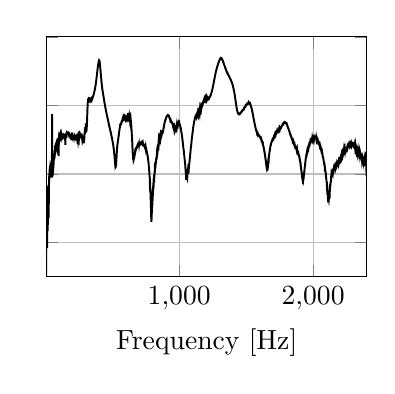
\begin{tikzpicture}

\begin{axis}[%
width=1.6in,
height=1.2in,
at={(1.011in,0.642in)},
scale only axis,
xmin=10,
xmax=2400,
xmajorgrids,
ymin=-30,
ymax=40,
ymajorgrids,
yticklabels={\empty},
xlabel={Frequency [Hz]},
axis background/.style={fill=white}
]
\addplot [color=black,solid,line width=0.7pt,forget plot]
  table[row sep=crcr]{%
0	-24.0538354294157\\
0.666675926054529	-24.7753265988161\\
1.33335185210906	-17.0382142167054\\
2.00002777816359	-18.7091958464009\\
2.66670370421811	-15.2032203403674\\
3.33337963027264	-8.53240216903954\\
4.00005555632717	-11.3881994991362\\
4.6667314823817	-7.34560264257265\\
5.33340740843623	-18.2635506378542\\
6.00008333449076	-30.0942089020284\\
6.66675926054529	-19.9100525240877\\
7.33343518659981	-21.3301429245582\\
8.00011111265434	-12.5504612701741\\
8.66678703870887	-15.3173206273707\\
9.3334629647634	-16.4624344447724\\
10.0001388908179	-21.0645945373479\\
10.6668148168725	-3.12818941832146\\
11.333490742927	-11.9814488880043\\
12.0001666689815	-16.3022691455521\\
12.666842595036	-16.83987041645\\
13.3335185210906	-21.5899394615097\\
14.0001944471451	-13.7669096045867\\
14.6668703731996	-10.7405701876275\\
15.3335462992542	-15.2513158642638\\
16.0002222253087	-12.4863764223308\\
16.6668981513632	-16.6735097060995\\
17.3335740774177	-11.1717261599997\\
18.0002500034723	-12.5642528883313\\
18.6669259295268	-14.7472480345922\\
19.3336018555813	-11.2309845901286\\
20.0002777816359	-12.3162845124428\\
20.6669537076904	-11.4989738149538\\
21.3336296337449	-11.4096075000397\\
22.0003055597994	-9.12000474667151\\
22.666981485854	-10.7058004870771\\
23.3336574119085	-10.8809274726073\\
24.000333337963	-12.8662435001899\\
24.6670092640176	-11.8084750036958\\
25.3336851900721	-9.39395341959846\\
26.0003611161266	-8.24921214045294\\
26.6670370421811	-5.13381010519183\\
27.3337129682357	-3.18474239145848\\
28.0003888942902	-1.96722097075604\\
28.6670648203447	-0.784435151267227\\
29.3337407463993	-0.564906469804107\\
30.0004166724538	-0.186628957762319\\
30.6670925985083	-0.223251397409185\\
31.3337685245628	-0.504288220825217\\
32.0004444506174	0.568981042424691\\
32.6671203766719	1.35135500831269\\
33.3337963027264	2.07752313968372\\
34.000472228781	2.13542686965292\\
34.6671481548355	1.87531635457994\\
35.33382408089	1.39408656672323\\
36.0005000069445	1.73767859557768\\
36.6671759329991	2.0365044287877\\
37.3338518590536	1.89103926658294\\
38.0005277851081	2.35267884483987\\
38.6672037111627	1.56785421692384\\
39.3338796372172	1.90575107773699\\
40.0005555632717	2.00696032260007\\
40.6672314893262	1.03747920044889\\
41.3339074153808	1.17819088709842\\
42.0005833414353	0.954423868100655\\
42.6672592674898	1.30215992319235\\
43.3339351935444	0.350798652357415\\
44.0006111195989	0.985446439692533\\
44.6672870456534	0.90853396189502\\
45.3339629717079	0.62363591607582\\
46.0006388977625	-0.106343649210524\\
46.667314823817	0.831296333741743\\
47.3339907498715	-0.154770617292899\\
48.0006666759261	-1.02488609973931\\
48.6673426019806	-0.349480793537451\\
49.3340185280351	1.40704941488586\\
50.0006944540896	17.4718617826514\\
50.6673703801442	-0.110905813330712\\
51.3340463061987	-0.969659382628823\\
52.0007222322532	-0.0156867446368573\\
52.6673981583078	-0.551828701230483\\
53.3340740843623	-0.335862030640212\\
54.0007500104168	-0.335709857720363\\
54.6674259364713	0.0689743844497208\\
55.3341018625259	0.149551305724914\\
56.0007777885804	0.650309261837628\\
56.6674537146349	0.13127845032964\\
57.3341296406895	0.572893104113807\\
58.000805566744	1.62672333434496\\
58.6674814927985	1.26340437511365\\
59.334157418853	1.80899399010958\\
60.0008333449076	2.12981393976939\\
60.6675092709621	2.11650037311116\\
61.3341851970166	2.70708359394901\\
62.0008611230712	3.0904031747816\\
62.6675370491257	3.73986090672288\\
63.3342129751802	4.11330532821165\\
64.0008889012347	4.28674048448287\\
64.6675648272893	4.49035790210038\\
65.3342407533438	4.62847704213878\\
66.0009166793983	4.90198327452499\\
66.6675926054529	5.40008752071958\\
67.3342685315074	5.71703775555609\\
68.0009444575619	5.85097210178158\\
68.6676203836164	6.35761681680145\\
69.334296309671	6.08420980880188\\
70.0009722357255	6.64342923814009\\
70.66764816178	7.14135937639171\\
71.3343240878346	6.95464466848458\\
72.0010000138891	7.3129468105897\\
72.6676759399436	7.26459405404091\\
73.3343518659981	7.48955717792348\\
74.0010277920527	7.65281470189807\\
74.6677037181072	7.55994571809288\\
75.3343796441617	7.89864326786307\\
76.0010555702163	7.63565632099739\\
76.6677314962708	7.89041771858883\\
77.3344074223253	7.83096423098779\\
78.0010833483798	7.95135021906428\\
78.6677592744344	8.15539545641694\\
79.3344352004889	8.08097874440249\\
80.0011111265434	8.18021272365017\\
80.667787052598	8.07561638981303\\
81.3344629786525	8.25782290136518\\
82.001138904707	8.02073159088786\\
82.6678148307615	8.42045087216576\\
83.3344907568161	8.1720438868478\\
84.0011666828706	8.11684485463587\\
84.6678426089251	8.2417824677993\\
85.3345185349797	8.26712476535566\\
86.0011944610342	8.08504729168952\\
86.6678703870887	8.39789867716215\\
87.3345463131432	8.45805928829301\\
88.0012222391978	8.62377756428815\\
88.6678981652523	8.52135557057066\\
89.3345740913068	8.67286525798598\\
90.0012500173614	8.85355762434988\\
90.6679259434159	9.00674645844902\\
91.3346018694704	9.00323229748388\\
92.0012777955249	9.23116144689982\\
92.6679537215795	9.19999321913624\\
93.334629647634	9.50702604628386\\
94.0013055736885	9.45354688509768\\
94.667981499743	9.60383675740148\\
95.3346574257976	9.70982758186113\\
96.0013333518521	9.81285612358788\\
96.6680092779066	9.87638222161103\\
97.3346852039612	9.98483507794277\\
98.0013611300157	10.2942179709114\\
98.6680370560702	10.0031320006568\\
99.3347129821248	10.234773264154\\
100.001388908179	5.20184010335849\\
100.668064834234	10.3673215378573\\
101.334740760288	10.6274246360448\\
102.001416686343	10.4963515327758\\
102.668092612397	10.6542180163706\\
103.334768538452	10.7270778119256\\
104.001444464506	10.7819900241968\\
104.668120390561	10.7476723911233\\
105.334796316616	10.8325568137231\\
106.00147224267	10.8565506329254\\
106.668148168725	10.7596885055515\\
107.334824094779	10.8153760411215\\
108.001500020834	10.9762515491244\\
108.668175946888	10.8813195235123\\
109.334851872943	10.9925472761605\\
110.001527798997	10.9839929711865\\
110.668203725052	10.8686273624886\\
111.334879651106	11.0336623311015\\
112.001555577161	10.8730227732298\\
112.668231503215	10.9764025968798\\
113.33490742927	10.9983924451575\\
114.001583355324	10.9932925852229\\
114.668259281379	10.8960860250767\\
115.334935207433	11.0971781560784\\
116.001611133488	10.9225306848365\\
116.668287059542	11.0012243151441\\
117.334962985597	10.9648906846422\\
118.001638911652	10.9810263450442\\
118.668314837706	10.9379766425556\\
119.334990763761	11.1180725359593\\
120.001666689815	10.8929973912361\\
120.66834261587	11.0346640034571\\
121.335018541924	11.0481488291843\\
122.001694467979	10.9418186978645\\
122.668370394033	10.9612899966686\\
123.335046320088	11.0949368089496\\
124.001722246142	11.0275110263947\\
124.668398172197	11.0715594833017\\
125.335074098251	11.0376539663672\\
126.001750024306	11.0892758690246\\
126.66842595036	10.9886866530624\\
127.335101876415	11.0544953488913\\
128.001777802469	11.086336614077\\
128.668453728524	11.0865827205247\\
129.335129654579	11.151384248337\\
130.001805580633	10.9699624040942\\
130.668481506688	11.0483383214513\\
131.335157432742	10.9434165920957\\
132.001833358797	10.9841995342106\\
132.668509284851	10.9498354463623\\
133.335185210906	11.0340101655261\\
134.00186113696	11.029981192541\\
134.668537063015	11.0002931400599\\
135.335212989069	11.0204717300212\\
136.001888915124	11.1082018634322\\
136.668564841178	11.1568604863805\\
137.335240767233	11.1212185688567\\
138.001916693287	11.1294445155704\\
138.668592619342	11.1038752994809\\
139.335268545396	10.9998777913079\\
140.001944471451	11.1203026571863\\
140.668620397506	11.0733110543624\\
141.33529632356	11.0783161713784\\
142.001972249615	11.2439397643653\\
142.668648175669	11.2245715123987\\
143.335324101724	11.2391735719326\\
144.002000027778	11.1714848438515\\
144.668675953833	11.2026579366728\\
145.335351879887	11.2800097757605\\
146.002027805942	11.2495634076332\\
146.668703731996	11.2875569503243\\
147.335379658051	11.2471604174122\\
148.002055584105	11.1433818238356\\
148.66873151016	11.1388023114834\\
149.335407436214	11.1083861020826\\
150.002083362269	8.49741873996997\\
150.668759288323	11.1444882241036\\
151.335435214378	11.0005689822991\\
152.002111140433	11.09039658558\\
152.668787066487	10.8554925363678\\
153.335462992542	10.8230173346571\\
154.002138918596	10.7685161320987\\
154.668814844651	10.8025435798439\\
155.335490770705	10.8135716851329\\
156.00216669676	10.8884190427297\\
156.668842622814	10.9438115197653\\
157.335518548869	11.108803501707\\
158.002194474923	11.3144993317585\\
158.668870400978	11.4290657039367\\
159.335546327032	11.5481305271641\\
160.002222253087	11.6743280140396\\
160.668898179141	11.5883742832391\\
161.335574105196	11.7607504814805\\
162.00225003125	11.7807862470171\\
162.668925957305	11.7467331034677\\
163.335601883359	11.7720285142441\\
164.002277809414	11.865060510984\\
164.668953735469	11.8803413440672\\
165.335629661523	11.8496811571761\\
166.002305587578	11.8324429598668\\
166.668981513632	11.8667775954332\\
167.335657439687	11.8685622372693\\
168.002333365741	11.9232402284661\\
168.669009291796	11.8631809517039\\
169.33568521785	11.8759285605512\\
170.002361143905	11.8500965787323\\
170.669037069959	11.8571411550248\\
171.335712996014	11.840672603201\\
172.002388922068	11.8726577669399\\
172.669064848123	11.8533596087701\\
173.335740774177	11.8970916548876\\
174.002416700232	11.8468821113692\\
174.669092626286	11.734120995521\\
175.335768552341	11.8545513954528\\
176.002444478396	11.8158272749587\\
176.66912040445	11.7581664010188\\
177.335796330505	11.6836690090809\\
178.002472256559	11.6134801753138\\
178.669148182614	11.545810162315\\
179.335824108668	11.580584591223\\
180.002500034723	11.4595817698421\\
180.669175960777	11.4109370365664\\
181.335851886832	11.4412280239627\\
182.002527812886	11.3337838862883\\
182.669203738941	11.2999958705124\\
183.335879664995	11.1766744105449\\
184.00255559105	11.2423046356787\\
184.669231517104	11.1506457429113\\
185.335907443159	11.049732946448\\
186.002583369213	11.0348385490678\\
186.669259295268	10.9294966777896\\
187.335935221323	10.9572626544397\\
188.002611147377	10.8441491005265\\
188.669287073432	10.7614007006402\\
189.335962999486	10.8383622788044\\
190.002638925541	10.8223907753729\\
190.669314851595	10.7318338151655\\
191.33599077765	10.7100341320297\\
192.002666703704	10.7954568913161\\
192.669342629759	10.7139401669828\\
193.336018555813	10.713553310691\\
194.002694481868	10.635326664087\\
194.669370407922	10.6914812192458\\
195.336046333977	10.6304543558945\\
196.002722260031	10.5135925535991\\
196.669398186086	10.4715652095356\\
197.33607411214	10.5958860446936\\
198.002750038195	10.5306409463711\\
198.66942596425	10.4646703088243\\
199.336101890304	10.6092591671541\\
200.002777816359	12.176381241264\\
200.669453742413	10.2229758071463\\
201.336129668468	10.4153000149645\\
202.002805594522	10.3409691366951\\
202.669481520577	10.3235299169775\\
203.336157446631	10.3908025729026\\
204.002833372686	10.4138955910993\\
204.66950929874	10.3096744183899\\
205.336185224795	10.3453530804593\\
206.002861150849	10.3411853460071\\
206.669537076904	10.4480086525697\\
207.336213002958	10.4821232768291\\
208.002888929013	10.4782237851814\\
208.669564855067	10.4857169071064\\
209.336240781122	10.5311820067122\\
210.002916707176	10.4065344665566\\
210.669592633231	10.3923410309562\\
211.336268559286	10.6125002075106\\
212.00294448534	10.6536877422631\\
212.669620411395	10.7075804710469\\
213.336296337449	10.5876450829407\\
214.002972263504	10.785798510488\\
214.669648189558	10.7575411253791\\
215.336324115613	10.8579433895683\\
216.003000041667	10.7564385534333\\
216.669675967722	10.8042910533961\\
217.336351893776	10.8590732035752\\
218.003027819831	10.9682998268144\\
218.669703745885	11.0298691531318\\
219.33637967194	10.9137424231625\\
220.003055597994	10.9268202865757\\
220.669731524049	11.1075459985888\\
221.336407450103	11.075272216335\\
222.003083376158	11.086723169469\\
222.669759302213	11.0306575287198\\
223.336435228267	11.0403269613152\\
224.003111154322	11.0461550610758\\
224.669787080376	10.8987251166676\\
225.336463006431	11.0093707380612\\
226.003138932485	11.0240270702722\\
226.66981485854	10.9899016358706\\
227.336490784594	10.8944098283972\\
228.003166710649	10.9776206027929\\
228.669842636703	10.9736768644323\\
229.336518562758	10.8881763913664\\
230.003194488812	10.8147798963354\\
230.669870414867	10.8177980422617\\
231.336546340921	10.8801157606152\\
232.003222266976	10.7283892320993\\
232.66989819303	10.6923124365478\\
233.336574119085	10.6786896011715\\
234.00325004514	10.4897476958619\\
234.669925971194	10.404416602913\\
235.336601897249	10.4085737009613\\
236.003277823303	10.3496630498464\\
236.669953749358	10.1939045392367\\
237.336629675412	10.3169473114109\\
238.003305601467	10.1109290157154\\
238.669981527521	10.0248242509185\\
239.336657453576	10.1248539008033\\
240.00333337963	9.86436784106379\\
240.670009305685	9.8461708563927\\
241.336685231739	9.80195907429479\\
242.003361157794	9.64681516121719\\
242.670037083848	9.65408983891004\\
243.336713009903	9.64755097355667\\
244.003388935957	9.47436381574311\\
244.670064862012	9.69859835886352\\
245.336740788066	9.54318354785978\\
246.003416714121	9.49157196217345\\
246.670092640176	9.61708331200281\\
247.33676856623	9.50254143555163\\
248.003444492285	9.58131774016605\\
248.670120418339	9.64528546865235\\
249.336796344394	9.58633365463329\\
250.003472270448	12.4050619191467\\
250.670148196503	10.1242217578109\\
251.336824122557	10.2671567123367\\
252.003500048612	10.562974536905\\
252.670175974666	10.6266234932955\\
253.336851900721	10.9711197026256\\
254.003527826775	10.9239309001141\\
254.67020375283	11.1999188615017\\
255.336879678884	11.1621178497936\\
256.003555604939	11.2330035027116\\
256.670231530993	11.3717480990161\\
257.336907457048	11.2397660539757\\
258.003583383103	11.3954434534165\\
258.670259309157	11.3330748055864\\
259.336935235212	11.4058114171549\\
260.003611161266	11.2727472424142\\
260.670287087321	11.3636069598555\\
261.336963013375	11.2803775781245\\
262.00363893943	11.3259731226633\\
262.670314865484	11.2831604198853\\
263.336990791539	11.2970077507477\\
264.003666717593	11.2537331196235\\
264.670342643648	11.2713568426248\\
265.337018569702	11.3038926896259\\
266.003694495757	11.1358976611144\\
266.670370421811	11.1288309856658\\
267.337046347866	11.0294360965846\\
268.00372227392	11.0311289283396\\
268.670398199975	11.0007018289668\\
269.33707412603	11.0526529539627\\
270.003750052084	10.9707716276467\\
270.670425978139	10.9747508530712\\
271.337101904193	10.6875614006601\\
272.003777830248	10.6611130565119\\
272.670453756302	10.5717850048715\\
273.337129682357	10.5648078472567\\
274.003805608411	10.499670336142\\
274.670481534466	10.3345037671487\\
275.33715746052	10.3743864040961\\
276.003833386575	10.0797133188244\\
276.670509312629	10.1874548657822\\
277.337185238684	9.99716266636554\\
278.003861164738	10.1329365143356\\
278.670537090793	9.9044650867058\\
279.337213016847	9.90190216469012\\
280.003888942902	9.79109249278751\\
280.670564868956	9.69492326926132\\
281.337240795011	9.69363522684118\\
282.003916721066	9.65539655977496\\
282.67059264712	9.61784377633952\\
283.337268573175	9.46150954678035\\
284.003944499229	9.4282426236971\\
284.670620425284	9.38794458809271\\
285.337296351338	9.3152770019253\\
286.003972277393	9.25769508223686\\
286.670648203447	9.19487404101757\\
287.337324129502	9.19501777667553\\
288.004000055556	9.35798780902652\\
288.670675981611	9.49456436606766\\
289.337351907665	9.7814876541983\\
290.00402783372	9.98147689201293\\
290.670703759774	10.2208175989873\\
291.337379685829	10.7311048602494\\
292.004055611883	11.0344757195201\\
292.670731537938	11.5192982400905\\
293.337407463993	11.8743752751125\\
294.004083390047	12.193556622589\\
294.670759316102	12.5652111611462\\
295.337435242156	12.9287677400434\\
296.004111168211	13.1378622004779\\
296.670787094265	13.2747682449318\\
297.33746302032	13.4282695085721\\
298.004138946374	13.5102474369325\\
298.670814872429	13.5312473320591\\
299.337490798483	13.3928499746803\\
300.004166724538	12.9948684163598\\
300.670842650592	13.3480927038971\\
301.337518576647	13.2475020503163\\
302.004194502701	13.0146629162693\\
302.670870428756	12.9962216245747\\
303.33754635481	12.8169344827781\\
304.004222280865	12.6361683472883\\
304.67089820692	12.5235804864241\\
305.337574132974	12.5701827364406\\
306.004250059029	12.4868789069686\\
306.670925985083	12.52032409134\\
307.337601911138	12.6466781948824\\
308.004277837192	12.9524182617077\\
308.670953763247	13.1715673652573\\
309.337629689301	13.5704043890882\\
310.004305615356	14.1606552716047\\
310.67098154141	14.7443826657853\\
311.337657467465	15.338294799873\\
312.004333393519	16.1663799368635\\
312.671009319574	16.9192556224687\\
313.337685245628	17.6011943590241\\
314.004361171683	18.3488092168469\\
314.671037097737	19.0888640542677\\
315.337713023792	19.6139738831932\\
316.004388949847	20.137762039088\\
316.671064875901	20.6552163789144\\
317.337740801956	20.9438530908394\\
318.00441672801	21.2412621975858\\
318.671092654065	21.4919486764409\\
319.337768580119	21.5977339205972\\
320.004444506174	21.7344452957731\\
320.671120432228	21.8822169758041\\
321.337796358283	21.9017537206537\\
322.004472284337	21.9473771938291\\
322.671148210392	22.0123528794745\\
323.337824136446	21.9793451486636\\
324.004500062501	22.0386109699524\\
324.671175988555	22.0408994279567\\
325.33785191461	21.9463862242842\\
326.004527840664	21.9753419819211\\
326.671203766719	21.933473132491\\
327.337879692774	21.875025790672\\
328.004555618828	21.8993855851231\\
328.671231544883	21.8122241818433\\
329.337907470937	21.7672598455656\\
330.004583396992	21.732754647684\\
330.671259323046	21.6567658373683\\
331.337935249101	21.6943787143949\\
332.004611175155	21.6311949762639\\
332.67128710121	21.5903275519017\\
333.337963027264	21.6334126166854\\
334.004638953319	21.4963114789822\\
334.671314879373	21.5484005574098\\
335.337990805428	21.5199247030615\\
336.004666731482	21.4870156650135\\
336.671342657537	21.544078906322\\
337.338018583591	21.4763389952504\\
338.004694509646	21.5451236206611\\
338.671370435701	21.5002992156288\\
339.338046361755	21.4914266245329\\
340.00472228781	21.5414916462764\\
340.671398213864	21.4969145634654\\
341.338074139919	21.5806730359757\\
342.004750065973	21.5164955323163\\
342.671425992028	21.631180114211\\
343.338101918082	21.6280672198441\\
344.004777844137	21.6524481284436\\
344.671453770191	21.6925161231834\\
345.338129696246	21.684657990614\\
346.0048056223	21.7959021361112\\
346.671481548355	21.7503780623695\\
347.338157474409	21.8858944759259\\
348.004833400464	21.8359367974069\\
348.671509326518	21.9503421196585\\
349.338185252573	21.9392384364729\\
350.004861178627	22.3870856318804\\
350.671537104682	22.0939943700624\\
351.338213030737	22.1333651372974\\
352.004888956791	22.1859159985505\\
352.671564882846	22.2314050905983\\
353.3382408089	22.3277504526568\\
354.004916734955	22.3332928147098\\
354.671592661009	22.456914580025\\
355.338268587064	22.5116795513418\\
356.004944513118	22.6268407556826\\
356.671620439173	22.6579767266709\\
357.338296365227	22.7830279539719\\
358.004972291282	22.7855363418947\\
358.671648217336	22.9282977061801\\
359.338324143391	22.9552004342005\\
360.005000069445	23.0967482034254\\
360.6716759955	23.1375534974305\\
361.338351921554	23.2671336898219\\
362.005027847609	23.3418111710958\\
362.671703773664	23.4712828577667\\
363.338379699718	23.553824857098\\
364.005055625773	23.6818063134887\\
364.671731551827	23.7736665359105\\
365.338407477882	23.8530357605844\\
366.005083403936	23.9997124292131\\
366.671759329991	24.0838168121703\\
367.338435256045	24.2347500113039\\
368.0051111821	24.3173935102669\\
368.671787108154	24.4909965246874\\
369.338463034209	24.558499138546\\
370.005138960263	24.7636680115791\\
370.671814886318	24.8500775519553\\
371.338490812372	25.0340991190821\\
372.005166738427	25.1554181253712\\
372.671842664481	25.31138732569\\
373.338518590536	25.503138701614\\
374.005194516591	25.5945440661062\\
374.671870442645	25.8258923739692\\
375.3385463687	25.8781832785756\\
376.005222294754	26.1212069673736\\
376.671898220809	26.2359863801086\\
377.338574146863	26.4563924416597\\
378.005250072918	26.6378861199214\\
378.671925998972	26.8034489554332\\
379.338601925027	27.0717627153897\\
380.005277851081	27.212045496638\\
380.671953777136	27.4561675539983\\
381.33862970319	27.6365587895402\\
382.005305629245	27.8153213652563\\
382.671981555299	28.0774413338392\\
383.338657481354	28.2342218562877\\
384.005333407408	28.5087659524338\\
384.672009333463	28.7540223326795\\
385.338685259517	28.9316679728972\\
386.005361185572	29.2350413994742\\
386.672037111627	29.3966621511991\\
387.338713037681	29.641209895069\\
388.005388963736	29.9193384375346\\
388.67206488979	30.0889819929086\\
389.338740815845	30.3889089301848\\
390.005416741899	30.5834284748198\\
390.672092667954	30.7520419489202\\
391.338768594008	31.0253306189734\\
392.005444520063	31.1691438622083\\
392.672120446117	31.3805029492705\\
393.338796372172	31.6109791175107\\
394.005472298226	31.7088394068235\\
394.672148224281	31.8977166816165\\
395.338824150335	32.118590197554\\
396.00550007639	32.2250301442221\\
396.672176002444	32.4383969709178\\
397.338851928499	32.584372014053\\
398.005527854554	32.652834316717\\
398.672203780608	32.8554270618435\\
399.338879706663	32.9949422192336\\
400.005555632717	33.0478065427637\\
400.672231558772	33.1054097052581\\
401.338907484826	33.2000438623887\\
402.005583410881	33.1679382029102\\
402.672259336935	33.1553109660612\\
403.33893526299	33.148151872368\\
404.005611189044	33.0332835311622\\
404.672287115099	32.9205788736783\\
405.338963041153	32.810301879351\\
406.005638967208	32.5985487610059\\
406.672314893262	32.3851116469242\\
407.338990819317	32.2026022497992\\
408.005666745371	31.9559744308648\\
408.672342671426	31.6418704159758\\
409.339018597481	31.3864409761776\\
410.005694523535	31.1469497092695\\
410.67237044959	30.7977082329506\\
411.339046375644	30.4783875394015\\
412.005722301699	30.2433520025839\\
412.672398227753	29.9082916554792\\
413.339074153808	29.5561508893066\\
414.005750079862	29.2914123673672\\
414.672426005917	29.0006488166639\\
415.339101931971	28.6876653242218\\
416.005777858026	28.3640825702083\\
416.67245378408	28.0606596600821\\
417.339129710135	27.8503313282515\\
418.005805636189	27.5189732830465\\
418.672481562244	27.1808685798042\\
419.339157488298	26.9525030135891\\
420.005833414353	26.7409332472361\\
420.672509340407	26.4505140133333\\
421.339185266462	26.1373778956874\\
422.005861192517	25.9445242047876\\
422.672537118571	25.7238560344385\\
423.339213044626	25.5265166116736\\
424.00588897068	25.2491125724447\\
424.672564896735	25.0250081623613\\
425.339240822789	24.8974975226114\\
426.005916748844	24.7224643389561\\
426.672592674898	24.5006868441122\\
427.339268600953	24.3066994958521\\
428.005944527007	24.1462413550494\\
428.672620453062	24.0507375112873\\
429.339296379116	23.8892840468726\\
430.005972305171	23.6776851026303\\
430.672648231225	23.5099653059884\\
431.33932415728	23.3478236259535\\
432.006000083334	23.2364127595894\\
432.672676009389	23.1207612587907\\
433.339351935444	22.8959361913742\\
434.006027861498	22.7471931522182\\
434.672703787553	22.5433582405117\\
435.339379713607	22.4547303842041\\
436.006055639662	22.2914653457661\\
436.672731565716	22.1519722574286\\
437.339407491771	21.9399191349777\\
438.006083417825	21.7290116106934\\
438.67275934388	21.5988691511031\\
439.339435269934	21.4594341238752\\
440.006111195989	21.3562168861861\\
440.672787122043	21.144900900334\\
441.339463048098	20.9739586695309\\
442.006138974152	20.7736080862848\\
442.672814900207	20.6201277638556\\
443.339490826261	20.5023998974435\\
444.006166752316	20.389707420288\\
444.672842678371	20.2221190500421\\
445.339518604425	20.1150004192628\\
446.00619453048	19.8958868027358\\
446.672870456534	19.7185496925901\\
447.339546382589	19.5946554813454\\
448.006222308643	19.4447782425543\\
448.672898234698	19.3248187746355\\
449.339574160752	19.2415878026817\\
450.006250086807	19.1969702927045\\
450.672926012861	18.9235712221156\\
451.339601938916	18.786476495092\\
452.00627786497	18.6138438464368\\
452.672953791025	18.458029742538\\
453.339629717079	18.3735391635682\\
454.006305643134	18.2274483277047\\
454.672981569188	18.1198667818157\\
455.339657495243	17.9970599081178\\
456.006333421298	17.9104914480584\\
456.673009347352	17.7908964404868\\
457.339685273407	17.6300876671202\\
458.006361199461	17.5205393224243\\
458.673037125516	17.3789005038587\\
459.33971305157	17.219497155265\\
460.006388977625	17.0916857427261\\
460.673064903679	16.967776133388\\
461.339740829734	16.8481704528801\\
462.006416755788	16.7606037216756\\
462.673092681843	16.6287300042932\\
463.339768607897	16.5150807513815\\
464.006444533952	16.4335668264479\\
464.673120460006	16.3541986927064\\
465.339796386061	16.2444898512573\\
466.006472312115	16.1022276577805\\
466.67314823817	16.0099998689133\\
467.339824164225	15.8321201445416\\
468.006500090279	15.731463989389\\
468.673176016334	15.598667407565\\
469.339851942388	15.4434925118285\\
470.006527868443	15.3418255048297\\
470.673203794497	15.260400829156\\
471.339879720552	15.1028294124931\\
472.006555646606	14.9703269586253\\
472.673231572661	14.8720922816024\\
473.339907498715	14.7048017505083\\
474.00658342477	14.6348712133549\\
474.673259350824	14.5046704313732\\
475.339935276879	14.3409902316396\\
476.006611202933	14.2909428993713\\
476.673287128988	14.1090275349316\\
477.339963055042	13.9893366679867\\
478.006638981097	13.9396784257778\\
478.673314907152	13.8030625702837\\
479.339990833206	13.6464528292807\\
480.006666759261	13.6262442302645\\
480.673342685315	13.4337902085009\\
481.34001861137	13.2908180780304\\
482.006694537424	13.2238446919687\\
482.673370463479	13.1087385153536\\
483.340046389533	12.9774902252141\\
484.006722315588	12.9235558923937\\
484.673398241642	12.7797322506448\\
485.340074167697	12.6652555108802\\
486.006750093751	12.5296361654673\\
486.673426019806	12.4705219488855\\
487.34010194586	12.3409420524972\\
488.006777871915	12.1918314613151\\
488.673453797969	12.1237800371845\\
489.340129724024	12.1137693010676\\
490.006805650078	11.9399408447004\\
490.673481576133	11.7769438523611\\
491.340157502188	11.6521991299404\\
492.006833428242	11.5335559889926\\
492.673509354297	11.3711021779641\\
493.340185280351	11.2797519092352\\
494.006861206406	11.1450543787188\\
494.67353713246	11.0490224157538\\
495.340213058515	10.8802703470087\\
496.006888984569	10.6657933239491\\
496.673564910624	10.639583194267\\
497.340240836678	10.5331311702954\\
498.006916762733	10.4376658346226\\
498.673592688787	10.226261189877\\
499.340268614842	10.173280789518\\
500.006944540896	9.97658207157796\\
500.673620466951	9.93104255542565\\
501.340296393005	9.70299151470093\\
502.00697231906	9.56427842467682\\
502.673648245115	9.40966460679045\\
503.340324171169	9.23208529134278\\
504.007000097224	9.16591247293168\\
504.673676023278	9.02470332922051\\
505.340351949333	8.85799847535677\\
506.007027875387	8.68232112750533\\
506.673703801442	8.49015542367151\\
507.340379727496	8.35612313467402\\
508.007055653551	8.09827396310981\\
508.673731579605	7.95619332879397\\
509.34040750566	7.71668486249847\\
510.007083431714	7.54408425757578\\
510.673759357769	7.3866368832407\\
511.340435283823	7.20454326168255\\
512.007111209878	6.96606098465922\\
512.673787135932	6.72619901342163\\
513.340463061987	6.33214482749454\\
514.007138988041	6.09664452506388\\
514.673814914096	6.00821140207314\\
515.340490840151	5.68996033058963\\
516.007166766205	5.41891292066807\\
516.67384269226	5.19913029101021\\
517.340518618314	4.74641232196898\\
518.007194544369	4.44353283286356\\
518.673870470423	4.18881886188834\\
519.340546396478	3.84761742946598\\
520.007222322532	3.53418988119992\\
520.673898248587	3.14939886494411\\
521.340574174641	2.838292842742\\
522.007250100696	2.57379153395263\\
522.67392602675	2.68621460723454\\
523.340601952805	2.54268561550195\\
524.007277878859	2.44119387057222\\
524.673953804914	2.34546990210759\\
525.340629730968	2.12788718992\\
526.007305657023	2.17247785298671\\
526.673981583078	2.17437754975731\\
527.340657509132	2.30955463293454\\
528.007333435187	2.32552210191851\\
528.674009361241	2.56150916661386\\
529.340685287296	3.1056710717391\\
530.00736121335	3.77675628169621\\
530.674037139405	4.23542156703512\\
531.340713065459	4.5715970853357\\
532.007388991514	4.98174110027376\\
532.674064917568	5.72223246797755\\
533.340740843623	6.01634248893307\\
534.007416769677	6.40373719646523\\
534.674092695732	6.81682238561117\\
535.340768621786	7.17875928125927\\
536.007444547841	7.47873462105253\\
536.674120473896	7.80929354526687\\
537.34079639995	8.05245706986005\\
538.007472326005	8.36022547474432\\
538.674148252059	8.58557421707928\\
539.340824178114	8.81462764879022\\
540.007500104168	8.93724767281927\\
540.674176030223	9.30767053508195\\
541.340851956277	9.41314167146452\\
542.007527882332	9.55514198421905\\
542.674203808386	9.80504696603795\\
543.340879734441	10.0715779624224\\
544.007555660495	10.1903989708205\\
544.67423158655	10.3261730853789\\
545.340907512604	10.5231373859331\\
546.007583438659	10.7373606145697\\
546.674259364713	10.8528441788335\\
547.340935290768	11.0243072468929\\
548.007611216823	11.3312786158819\\
548.674287142877	11.3774764740178\\
549.340963068932	11.6524856563262\\
550.007638994986	11.8209336106523\\
550.674314921041	12.0719428085404\\
551.340990847095	12.174427441001\\
552.00766677315	12.4054022511678\\
552.674342699204	12.675640934017\\
553.341018625259	12.8103604363372\\
554.007694551313	12.9886014144124\\
554.674370477368	13.1767125315813\\
555.341046403422	13.3030478639295\\
556.007722329477	13.4715164884348\\
556.674398255531	13.7083858707781\\
557.341074181586	13.7995387628935\\
558.00775010764	13.9282687496593\\
558.674426033695	14.2224926371625\\
559.341101959749	14.2258110595647\\
560.007777885804	14.3252407459023\\
560.674453811858	14.5106403874977\\
561.341129737913	14.5096064949592\\
562.007805663968	14.5862548783372\\
562.674481590022	14.6686389667934\\
563.341157516077	14.668275787313\\
564.007833442131	14.7581885840426\\
564.674509368186	14.7889406640586\\
565.34118529424	14.7330637771831\\
566.007861220295	14.7761720485605\\
566.674537146349	14.7950379349273\\
567.341213072404	14.8136528998632\\
568.007888998458	14.9307479037634\\
568.674564924513	14.8869093992123\\
569.341240850567	15.0020057804691\\
570.007916776622	15.0448899036403\\
570.674592702676	15.0733428753757\\
571.341268628731	15.2653123767828\\
572.007944554785	15.2859544262324\\
572.67462048084	15.3244107965716\\
573.341296406895	15.5056585597125\\
574.007972332949	15.5463222031134\\
574.674648259004	15.7091986008417\\
575.341324185058	15.7857704631097\\
576.008000111113	15.8942386542656\\
576.674676037167	16.0257081173392\\
577.341351963222	16.0149498355079\\
578.008027889276	16.1879588740618\\
578.674703815331	16.1729269420844\\
579.341379741385	16.3083726802466\\
580.00805566744	16.3575588369278\\
580.674731593494	16.365937703832\\
581.341407519549	16.4928648069782\\
582.008083445603	16.4135098039103\\
582.674759371658	16.5606232989547\\
583.341435297712	16.4949869606825\\
584.008111223767	16.5875942777116\\
584.674787149822	16.5514655794609\\
585.341463075876	16.5654555789107\\
586.008139001931	16.6053193123706\\
586.674814927985	16.5052009636011\\
587.34149085404	16.6072309414191\\
588.008166780094	16.4786187578352\\
588.674842706149	16.5574939792168\\
589.341518632203	16.4367798218283\\
590.008194558258	16.4995798511669\\
590.674870484312	16.3865012367849\\
591.341546410367	16.4592085148972\\
592.008222336421	16.340487948373\\
592.674898262476	16.3670572759151\\
593.34157418853	16.3063615038774\\
594.008250114585	16.3455728584197\\
594.674926040639	16.2608916229011\\
595.341601966694	16.297350941732\\
596.008277892749	16.2025084546167\\
596.674953818803	16.2378002755367\\
597.341629744858	16.1963992046452\\
598.008305670912	16.1688825705917\\
598.674981596967	16.1131426357601\\
599.341657523021	16.2063396706033\\
600.008333449076	16.082470288651\\
600.67500937513	16.1749020334652\\
601.341685301185	16.1246008212953\\
602.008361227239	16.1984115744638\\
602.675037153294	16.0948019285334\\
603.341713079348	16.2170131537778\\
604.008389005403	16.1304315172695\\
604.675064931457	16.2492579274956\\
605.341740857512	16.1712036728509\\
606.008416783566	16.2362173440111\\
606.675092709621	16.2120105909438\\
607.341768635676	16.3022758438576\\
608.00844456173	16.2397755587875\\
608.675120487785	16.3371921941228\\
609.341796413839	16.3336724777239\\
610.008472339894	16.3313353363035\\
610.675148265948	16.3979196428623\\
611.341824192003	16.3129768461316\\
612.008500118057	16.4385269611059\\
612.675176044112	16.3194257948107\\
613.341851970166	16.4457013711349\\
614.008527896221	16.4065585931307\\
614.675203822275	16.4363597931761\\
615.34187974833	16.507449764277\\
616.008555674384	16.4506796275132\\
616.675231600439	16.5520510315926\\
617.341907526493	16.4627257345375\\
618.008583452548	16.624553047341\\
618.675259378603	16.5335960648416\\
619.341935304657	16.5616368108617\\
620.008611230711	16.636736390542\\
620.675287156766	16.5478634227533\\
621.341963082821	16.6756072286469\\
622.008639008875	16.5836004908967\\
622.67531493493	16.6108910965367\\
623.341990860984	16.6894703602389\\
624.008666787039	16.5677177530767\\
624.675342713093	16.6913117157591\\
625.342018639148	16.6488815610008\\
626.008694565202	16.5487677436973\\
626.675370491257	16.7555897507216\\
627.342046417311	16.55274074888\\
628.008722343366	16.5611432576366\\
628.67539826942	16.6416552804713\\
629.342074195475	16.4320030957751\\
630.008750121529	16.5406189712251\\
630.675426047584	16.580535623175\\
631.342101973638	16.267797586175\\
632.008777899693	16.4726226747189\\
632.675453825748	16.4025795355512\\
633.342129751802	16.1751980714638\\
634.008805677857	16.2920847485297\\
634.675481603911	16.0718224148971\\
635.342157529966	15.9247024759311\\
636.00883345602	16.0239536112237\\
636.675509382075	15.799687708656\\
637.342185308129	15.4575806981259\\
638.008861234184	15.6327066208098\\
638.675537160238	15.3118732652641\\
639.342213086293	14.8517393760472\\
640.008889012347	14.9662407330703\\
640.675564938402	14.7259462068026\\
641.342240864456	14.1296834286275\\
642.008916790511	13.9712980107766\\
642.675592716565	13.9101024775435\\
643.34226864262	13.1266704172734\\
644.008944568675	12.8538851703094\\
644.675620494729	12.7481594386484\\
645.342296420784	11.9965695483298\\
646.008972346838	11.4499069847361\\
646.675648272893	11.2990796911129\\
647.342324198947	10.7009231507117\\
648.009000125002	9.88953406030728\\
648.675676051056	9.50168700273076\\
649.342351977111	9.10954130375459\\
650.009027903165	8.64820776820932\\
650.67570382922	7.61756872242853\\
651.342379755274	7.40586741417076\\
652.009055681329	7.08942540282487\\
652.675731607383	6.08200626385361\\
653.342407533438	5.72419650143808\\
654.009083459492	5.49759242816381\\
654.675759385547	5.29169501571504\\
655.342435311602	4.71109730366877\\
656.009111237656	4.29505478873706\\
656.675787163711	4.61234146286363\\
657.342463089765	4.51977411033579\\
658.00913901582	4.24545086492994\\
658.675814941874	3.99616888525082\\
659.342490867929	4.07913016147592\\
660.009166793983	4.43900944385735\\
660.675842720038	4.38012170617682\\
661.342518646092	4.4514484809695\\
662.009194572147	4.55053847636848\\
662.675870498201	4.68581788631672\\
663.342546424256	5.06836396711243\\
664.00922235031	5.03834687003778\\
664.675898276365	5.01798182971722\\
665.342574202419	5.29255886284392\\
666.009250128474	5.57963088869587\\
666.675926054529	5.70082816841368\\
667.342601980583	5.66047564216475\\
668.009277906638	5.65110414379459\\
668.675953832692	6.05820324551451\\
669.342629758747	6.26256346656145\\
670.009305684801	6.18875699485358\\
670.675981610856	6.26566083216555\\
671.34265753691	6.37375958455085\\
672.009333462965	6.46899287385204\\
672.676009389019	6.7023481501977\\
673.342685315074	6.92994514722064\\
674.009361241128	6.9142441838001\\
674.676037167183	6.84390413844429\\
675.342713093237	6.93362228437308\\
676.009389019292	7.16013982468008\\
676.676064945346	7.29782724821155\\
677.342740871401	7.28099887468422\\
678.009416797456	7.28553560396656\\
678.67609272351	7.3438589447758\\
679.342768649565	7.35268456383873\\
680.009444575619	7.46013201228345\\
680.676120501674	7.58787823875755\\
681.342796427728	7.70987056832242\\
682.009472353783	7.7047698036689\\
682.676148279837	7.71836181754712\\
683.342824205892	7.71287810866602\\
684.009500131946	7.88491955520567\\
684.676176058001	7.88200458566801\\
685.342851984055	7.97871547719071\\
686.00952791011	8.06262035838028\\
686.676203836164	8.19454833038218\\
687.342879762219	8.16680871449154\\
688.009555688273	8.14986629672043\\
688.676231614328	8.11098997869995\\
689.342907540382	8.15600053376475\\
690.009583466437	8.2431174413041\\
690.676259392492	8.35857584547801\\
691.342935318546	8.47980551964391\\
692.009611244601	8.43020986419829\\
692.676287170655	8.48780149220811\\
693.34296309671	8.49475492350756\\
694.009639022764	8.48315887279011\\
694.676314948819	8.50345618383611\\
695.342990874873	8.48156685248925\\
696.009666800928	8.6273150299049\\
696.676342726982	8.65591179059107\\
697.343018653037	8.66517613107\\
698.009694579091	8.77821021920323\\
698.676370505146	8.75333557717898\\
699.3430464312	8.8738621831423\\
700.009722357255	8.65908011082201\\
700.676398283309	8.86688296460674\\
701.343074209364	8.99292078768806\\
702.009750135419	8.92702794124702\\
702.676426061473	8.94314707926746\\
703.343101987528	9.00448341199101\\
704.009777913582	8.99974507269237\\
704.676453839637	8.94855984341114\\
705.343129765691	8.91491375340969\\
706.009805691746	9.04507061596649\\
706.6764816178	9.03253887450496\\
707.343157543855	9.0075023601351\\
708.009833469909	8.99718959363287\\
708.676509395964	9.10477017565572\\
709.343185322018	9.17907052885568\\
710.009861248073	9.18639911781509\\
710.676537174127	9.08239240901507\\
711.343213100182	9.16189627843021\\
712.009889026236	9.19475262476087\\
712.676564952291	9.2117120724423\\
713.343240878346	9.24617414557119\\
714.0099168044	9.28100228694381\\
714.676592730455	9.3022214295608\\
715.343268656509	9.21367630460709\\
716.009944582564	9.22161749744294\\
716.676620508618	9.20051200364815\\
717.343296434673	9.19917213365312\\
718.009972360727	9.20628728333848\\
718.676648286782	9.15288523255609\\
719.343324212836	9.18144019305628\\
720.010000138891	9.0888488044096\\
720.676676064945	9.13366907544728\\
721.343351991	9.09691399403723\\
722.010027917054	9.07780768358352\\
722.676703843109	8.99477464928745\\
723.343379769163	9.06415786331838\\
724.010055695218	8.9396147449063\\
724.676731621273	8.91679571829932\\
725.343407547327	8.89078643803618\\
726.010083473382	8.89081486731126\\
726.676759399436	8.86587058208948\\
727.343435325491	8.82387149713632\\
728.010111251545	8.84742213310955\\
728.6767871776	8.80797109096137\\
729.343463103654	8.77921127750227\\
730.010139029709	8.88600239733476\\
730.676814955763	8.76052369591128\\
731.343490881818	8.84503878959984\\
732.010166807872	8.78348576588829\\
732.676842733927	8.74729278566041\\
733.343518659981	8.69718510731511\\
734.010194586036	8.58765820005153\\
734.67687051209	8.55866789218656\\
735.343546438145	8.57966892515378\\
736.0102223642	8.51429485733572\\
736.676898290254	8.47576228049317\\
737.343574216309	8.47350178943034\\
738.010250142363	8.36534874926045\\
738.676926068418	8.3134314464271\\
739.343601994472	8.30784562333557\\
740.010277920527	8.30356706532026\\
740.676953846581	8.29810828413785\\
741.343629772636	8.28230145879134\\
742.01030569869	8.19757323542451\\
742.676981624745	8.16306820019938\\
743.343657550799	8.10197498872195\\
744.010333476854	7.91140718178206\\
744.677009402908	7.95146581159202\\
745.343685328963	7.89349505820059\\
746.010361255017	7.81561049766296\\
746.677037181072	7.91101046118437\\
747.343713107127	7.81549474148716\\
748.010389033181	7.79004878356179\\
748.677064959236	7.66829467356041\\
749.34374088529	7.49522738347616\\
750.010416811345	7.68306725636067\\
750.677092737399	7.47542347743726\\
751.343768663454	7.30539756747948\\
752.010444589508	7.32444285285847\\
752.677120515563	7.19256018569224\\
753.343796441617	7.22101513454485\\
754.010472367672	6.98367788213361\\
754.677148293726	6.94151082884162\\
755.343824219781	6.81920124364684\\
756.010500145835	6.85561208875995\\
756.67717607189	6.73901309068327\\
757.343851997944	6.65447059917736\\
758.010527923999	6.39940819849267\\
758.677203850054	6.31537062804607\\
759.343879776108	6.2304774693665\\
760.010555702162	6.15132302820454\\
760.677231628217	6.03645142947089\\
761.343907554272	5.82856391160883\\
762.010583480326	5.62639500122763\\
762.677259406381	5.49140195078828\\
763.343935332435	5.29501650067733\\
764.01061125849	5.28840291402563\\
764.677287184544	5.13659478264419\\
765.343963110599	4.92696956390757\\
766.010639036653	4.65854266888813\\
766.677314962708	4.49329801241826\\
767.343990888762	4.39946911523809\\
768.010666814817	4.1882380007889\\
768.677342740871	3.83121132007652\\
769.344018666926	3.6747490934063\\
770.01069459298	3.51415478445073\\
770.677370519035	3.36285311572927\\
771.344046445089	2.99118916014252\\
772.010722371144	2.83533387759084\\
772.677398297199	2.31556653261333\\
773.344074223253	2.18825393175463\\
774.010750149308	1.94755390900186\\
774.677426075362	1.30582271184568\\
775.344102001417	1.12798424630628\\
776.010777927471	1.11609012507506\\
776.677453853526	0.541390822703892\\
777.34412977958	0.158386409686359\\
778.010805705635	-0.468980051040267\\
778.677481631689	-0.714193168197218\\
779.344157557744	-0.899055137537588\\
780.010833483798	-1.07703919157975\\
780.677509409853	-2.49646867206346\\
781.344185335907	-2.37501600216951\\
782.010861261962	-2.17316165963422\\
782.677537188016	-4.0581005908558\\
783.344213114071	-4.58062890864723\\
784.010889040126	-4.58269787118991\\
784.67756496618	-4.7208140869024\\
785.344240892235	-5.73279953533563\\
786.010916818289	-6.89575411330063\\
786.677592744344	-6.68381994855648\\
787.344268670398	-8.18517020034133\\
788.010944596453	-9.90652762988221\\
788.677620522507	-8.18289582525946\\
789.344296448562	-10.1846467980253\\
790.010972374616	-12.5734242530755\\
790.677648300671	-11.2925063282194\\
791.344324226725	-11.0326681826804\\
792.01100015278	-13.9522799585502\\
792.677676078834	-10.6894138613858\\
793.344352004889	-11.2152910111612\\
794.011027930943	-13.2516412128331\\
794.677703856998	-9.79569996931918\\
795.344379783053	-11.3022395543273\\
796.011055709107	-11.4952272503209\\
796.677731635162	-8.41722339018986\\
797.344407561216	-9.72627220711398\\
798.011083487271	-9.94979243639554\\
798.677759413325	-6.87502790192122\\
799.34443533938	-9.12375254882056\\
800.011111265434	-7.32160601680179\\
800.677787191489	-5.43797021337587\\
801.344463117543	-7.80256595429727\\
802.011139043598	-5.13409187346906\\
802.677814969652	-4.94108863994887\\
803.344490895707	-6.37745787416539\\
804.011166821761	-3.55950243852837\\
804.677842747816	-4.30586109253226\\
805.34451867387	-4.59397551263602\\
806.011194599925	-2.73093805028424\\
806.67787052598	-4.50721520541811\\
807.344546452034	-2.71904955651304\\
808.011222378089	-2.56406630580553\\
808.677898304143	-3.79276753181882\\
809.344574230198	-1.43233406110157\\
810.011250156252	-2.40888422001714\\
810.677926082307	-2.26245578595983\\
811.344602008361	-1.04421395839191\\
812.011277934416	-2.49516241499997\\
812.67795386047	-0.268917971359419\\
813.344629786525	-1.44027205880575\\
814.011305712579	-0.58017509754626\\
814.677981638634	-0.106411658385477\\
815.344657564688	-0.604591426118682\\
816.011333490743	0.94649791000057\\
816.678009416797	-0.0135856302018601\\
817.344685342852	1.01227256578035\\
818.011361268907	0.874174188656179\\
818.678037194961	1.14296528929029\\
819.344713121016	1.83339816048708\\
820.01138904707	1.37241871192462\\
820.678064973125	2.35754556263054\\
821.344740899179	1.695533751534\\
822.011416825234	2.65437077751505\\
822.678092751288	2.33195299209198\\
823.344768677343	2.6712027563085\\
824.011444603397	3.12226968652874\\
824.678120529452	2.85017726099925\\
825.344796455506	3.68194181903176\\
826.011472381561	3.10750420962551\\
826.678148307615	4.10803459146397\\
827.34482423367	3.63804406996872\\
828.011500159724	4.50743894422469\\
828.678176085779	4.26625290414105\\
829.344852011833	4.5765990683043\\
830.011527937888	4.72375359303579\\
830.678203863943	4.97318854745414\\
831.344879789997	5.04487623377831\\
832.011555716052	5.21440337067422\\
832.678231642106	5.4887612967534\\
833.344907568161	5.62068819776284\\
834.011583494215	6.0910417712059\\
834.67825942027	5.98735626527823\\
835.344935346324	6.328626218188\\
836.011611272379	6.43646375962649\\
836.678287198433	6.7736958348463\\
837.344963124488	6.82165695424229\\
838.011639050542	7.19372361307892\\
838.678314976597	7.11523922481778\\
839.344990902651	7.57138139653562\\
840.011666828706	7.557247900819\\
840.67834275476	7.90611873433456\\
841.345018680815	7.91608176675178\\
842.01169460687	8.09851421262908\\
842.678370532924	8.3536357220389\\
843.345046458979	8.40510316993884\\
844.011722385033	8.67827879791309\\
844.678398311088	8.72842127719789\\
845.345074237142	9.06145967026124\\
846.011750163197	8.85824675407166\\
846.678426089251	9.33381122591847\\
847.345102015306	9.16247240374297\\
848.01177794136	9.53714993615979\\
848.678453867415	9.45222110064775\\
849.345129793469	9.75549204802832\\
850.011805719524	9.72011555940689\\
850.678481645578	9.80556141254699\\
851.345157571633	10.0157705307232\\
852.011833497687	9.98782400806894\\
852.678509423742	10.3263323152393\\
853.345185349797	10.2263075124648\\
854.011861275851	10.4673662333594\\
854.678537201906	10.4750122257284\\
855.34521312796	10.5812683543939\\
856.011889054015	10.7432021798873\\
856.678564980069	10.6224034655495\\
857.345240906124	10.8200206780487\\
858.011916832178	10.7909061950638\\
858.678592758233	10.9237707622318\\
859.345268684287	11.0856784961665\\
860.011944610342	10.8644352842758\\
860.678620536396	11.1261066554508\\
861.345296462451	11.0244524327826\\
862.011972388505	11.1470113009769\\
862.67864831456	11.2547196785471\\
863.345324240614	11.0448320287065\\
864.012000166669	11.2151192729638\\
864.678676092724	11.2531785369515\\
865.345352018778	11.2555770207634\\
866.012027944833	11.4987110031993\\
866.678703870887	11.4224990994646\\
867.345379796942	11.5779639905364\\
868.012055722996	11.640257357955\\
868.678731649051	11.6007867483666\\
869.345407575105	11.781237805192\\
870.01208350116	11.877495251888\\
870.678759427214	11.8489151436538\\
871.345435353269	12.0846483711101\\
872.012111279323	12.0525281222913\\
872.678787205378	12.0139984235166\\
873.345463131432	12.0826812209638\\
874.012139057487	12.061523307729\\
874.678814983541	12.1489753287143\\
875.345490909596	12.3037009790466\\
876.012166835651	12.3632402363005\\
876.678842761705	12.3976444803187\\
877.34551868776	12.5413102336594\\
878.012194613814	12.5428786333715\\
878.678870539869	12.5052739178201\\
879.345546465923	12.6803526763113\\
880.012222391978	12.7657815401847\\
880.678898318032	12.7619737549631\\
881.345574244087	12.9302223410476\\
882.012250170141	13.1298104776297\\
882.678926096196	13.1343444772437\\
883.34560202225	13.3622493754369\\
884.012277948305	13.516955430761\\
884.678953874359	13.628462736946\\
885.345629800414	13.7511746464535\\
886.012305726468	13.9753184008757\\
886.678981652523	14.1028982643568\\
887.345657578578	14.1752525376684\\
888.012333504632	14.4232471395254\\
888.679009430687	14.6262802091452\\
889.345685356741	14.6695853406587\\
890.012361282796	14.8377869147203\\
890.67903720885	14.9993208078014\\
891.345713134905	15.0808226015919\\
892.012389060959	15.1835072151555\\
892.679064987014	15.2992595795399\\
893.345740913068	15.4770778589417\\
894.012416839123	15.5313052994013\\
894.679092765177	15.5677504345894\\
895.345768691232	15.6845822811017\\
896.012444617286	15.7420524263474\\
896.679120543341	15.7676966606647\\
897.345796469395	15.7644520748567\\
898.01247239545	15.8820572624777\\
898.679148321504	15.9725363968445\\
899.345824247559	16.0137849317211\\
900.012500173613	16.085611690765\\
900.679176099668	16.1409539861349\\
901.345852025723	16.2961684756008\\
902.012527951777	16.3377643610367\\
902.679203877832	16.4297773781262\\
903.345879803886	16.4858328512957\\
904.012555729941	16.564890281754\\
904.679231655995	16.6877664339662\\
905.34590758205	16.7312284524711\\
906.012583508104	16.7491872727016\\
906.679259434159	16.8286310282731\\
907.345935360213	16.8741824254074\\
908.012611286268	16.9141639567492\\
908.679287212322	16.9528059124308\\
909.345963138377	17.0085270302337\\
910.012639064431	17.0507269149622\\
910.679314990486	17.0919263331357\\
911.34599091654	17.1157916064077\\
912.012666842595	17.1178820583425\\
912.67934276865	17.0880992386827\\
913.346018694704	17.1412446050638\\
914.012694620759	17.1206095613056\\
914.679370546813	17.157389034818\\
915.346046472868	17.1386740071617\\
916.012722398922	17.1253703278769\\
916.679398324977	17.1517005258387\\
917.346074251031	17.1273425555082\\
918.012750177086	17.1681988564691\\
918.67942610314	17.1485984223438\\
919.346102029195	17.1222604286733\\
920.012777955249	17.0702448417329\\
920.679453881304	17.0327124157506\\
921.346129807358	17.0239384095614\\
922.012805733413	16.9688121297861\\
922.679481659467	16.9417438457129\\
923.346157585522	16.9388097335481\\
924.012833511577	16.8382022700095\\
924.679509437631	16.7353323309267\\
925.346185363686	16.6337259820966\\
926.01286128974	16.5335111732478\\
926.679537215795	16.5419485621736\\
927.346213141849	16.511166162688\\
928.012889067904	16.4120307544702\\
928.679564993958	16.24589127645\\
929.346240920013	16.1829108978507\\
930.012916846067	16.0872592124875\\
930.679592772122	16.0621013310755\\
931.346268698176	16.0021972137655\\
932.012944624231	15.8295300378117\\
932.679620550285	15.7242468026111\\
933.34629647634	15.7594562496269\\
934.012972402394	15.7778623709336\\
934.679648328449	15.6435455070428\\
935.346324254504	15.4933174941697\\
936.013000180558	15.5246753676726\\
936.679676106613	15.5753115387579\\
937.346352032667	15.4429144622277\\
938.013027958722	15.3277309493187\\
938.679703884776	15.3420270995758\\
939.346379810831	15.3637397811101\\
940.013055736885	15.2954983471487\\
940.67973166294	15.2502892792833\\
941.346407588994	15.1915627950314\\
942.013083515049	15.2282875536802\\
942.679759441103	15.2407101106542\\
943.346435367158	15.1592809678109\\
944.013111293212	15.1304660578284\\
944.679787219267	15.1042989217109\\
945.346463145321	15.0981831699222\\
946.013139071376	15.0112536579602\\
946.679814997431	15.0087693252248\\
947.346490923485	14.9596905684958\\
948.01316684954	14.8097109633695\\
948.679842775594	14.7245500155753\\
949.346518701649	14.6901579331699\\
950.013194627703	14.6241894734558\\
950.679870553758	14.478281390526\\
951.346546479812	14.3752459245062\\
952.013222405867	14.3552520626441\\
952.679898331921	14.2506677012263\\
953.346574257976	14.0682417163199\\
954.01325018403	14.0975784558267\\
954.679926110085	13.9469010446043\\
955.346602036139	13.8041934037683\\
956.013277962194	13.8690848346785\\
956.679953888248	13.7182791326649\\
957.346629814303	13.6033379889394\\
958.013305740358	13.6693326390777\\
958.679981666412	13.4266508795005\\
959.346657592467	13.4388957881631\\
960.013333518521	13.4562971477598\\
960.680009444576	13.2648794684452\\
961.34668537063	13.3043235786423\\
962.013361296685	13.3016144305801\\
962.680037222739	13.1181477197663\\
963.346713148794	13.2833055336899\\
964.013389074848	13.1566306036221\\
964.680065000903	13.1504651053162\\
965.346740926957	13.2808770999398\\
966.013416853012	13.0452572936668\\
966.680092779066	13.1782410338397\\
967.346768705121	13.0510306040208\\
968.013444631175	13.0439535370866\\
968.68012055723	13.1034073989045\\
969.346796483284	12.9817057992295\\
970.013472409339	13.0806589806179\\
970.680148335394	12.9908520584691\\
971.346824261448	13.0908405195881\\
972.013500187503	13.1719572370936\\
972.680176113557	13.1217450297585\\
973.346852039612	13.2696216562191\\
974.013527965666	13.2079063705257\\
974.680203891721	13.3898792150133\\
975.346879817775	13.3401341277843\\
976.01355574383	13.454003479962\\
976.680231669884	13.4639679336425\\
977.346907595939	13.5210052363991\\
978.013583521993	13.5523703564507\\
978.680259448048	13.545590042943\\
979.346935374102	13.7013002274013\\
980.013611300157	13.6538033203134\\
980.680287226211	13.8649022715395\\
981.346963152266	13.8741479473683\\
982.013639078321	14.0982455357562\\
982.680315004375	13.9058036414396\\
983.34699093043	14.1382987320142\\
984.013666856484	14.1613000639855\\
984.680342782539	14.2588636401027\\
985.347018708593	14.2645946141291\\
986.013694634648	14.3277308803772\\
986.680370560702	14.3574066714178\\
987.347046486757	14.4917590223021\\
988.013722412811	14.4213472494812\\
988.680398338866	14.5951596860138\\
989.34707426492	14.5584482920297\\
990.013750190975	14.6344774420352\\
990.680426117029	14.5326826425877\\
991.347102043084	14.7218891457685\\
992.013777969138	14.7646012402875\\
992.680453895193	14.8554379744139\\
993.347129821248	14.8021957586984\\
994.013805747302	14.8348303921759\\
994.680481673357	14.8832926017775\\
995.347157599411	14.8653025353454\\
996.013833525466	14.9156060665405\\
996.68050945152	14.9169650687554\\
997.347185377575	15.0347524053791\\
998.013861303629	14.9599693289121\\
998.680537229684	14.8935861046312\\
999.347213155738	14.8986115671854\\
1000.01388908179	14.8020118876697\\
1000.68056500785	14.8603228393408\\
1001.3472409339	14.673035487848\\
1002.01391685996	14.6814363141461\\
1002.68059278601	14.6099511444209\\
1003.34726871207	14.4835362836934\\
1004.01394463812	14.4417018750116\\
1004.68062056417	14.3431173666552\\
1005.34729649023	14.2288320465421\\
1006.01397241628	14.1903962036071\\
1006.68064834234	14.0708621518306\\
1007.34732426839	13.9997619161669\\
1008.01400019445	13.9055538185116\\
1008.6806761205	13.7794447081556\\
1009.34735204656	13.5856489796792\\
1010.01402797261	13.6035024533102\\
1010.68070389867	13.4719844593725\\
1011.34737982472	13.3261108486719\\
1012.01405575077	13.1806152195859\\
1012.68073167683	13.1030103916831\\
1013.34740760288	13.00446888968\\
1014.01408352894	12.7690264204968\\
1014.68075945499	12.5902931535884\\
1015.34743538105	12.443154237171\\
1016.0141113071	12.320263731277\\
1016.68078723316	12.1579997892401\\
1017.34746315921	12.0538553052052\\
1018.01413908527	11.7780627530031\\
1018.68081501132	11.6624214031315\\
1019.34749093737	11.4572123788654\\
1020.01416686343	11.2988764691802\\
1020.68084278948	11.1476342740219\\
1021.34751871554	10.8474180244978\\
1022.01419464159	10.7243619002042\\
1022.68087056765	10.5018964508221\\
1023.3475464937	10.2652104129408\\
1024.01422241976	10.0276652031138\\
1024.68089834581	9.85412344754131\\
1025.34757427186	9.62364054797986\\
1026.01425019792	9.38024021757669\\
1026.68092612397	9.07955382760224\\
1027.34760205003	8.91495342322297\\
1028.01427797608	8.61132645977498\\
1028.68095390214	8.40917931755813\\
1029.34762982819	8.17485545980325\\
1030.01430575425	7.8696530528584\\
1030.6809816803	7.61042520669973\\
1031.34765760636	7.47194842875038\\
1032.01433353241	7.37439919173195\\
1032.68100945846	7.04569416826588\\
1033.34768538452	6.98871767438864\\
1034.01436131057	6.70330079806592\\
1034.68103723663	6.50286540580077\\
1035.34771316268	6.14159337203889\\
1036.01438908874	5.81152348911526\\
1036.68106501479	5.7720153358707\\
1037.34774094085	5.63190324881289\\
1038.0144168669	5.20546134010407\\
1038.68109279296	5.05775239691149\\
1039.34776871901	4.65424772134796\\
1040.01444464506	4.25396122764083\\
1040.68112057112	4.50080563258035\\
1041.34779649717	3.96017196085356\\
1042.01447242323	3.68542479499865\\
1042.68114834928	3.38789079565235\\
1043.34782427534	3.00066741929081\\
1044.01450020139	2.8699683570844\\
1044.68117612745	2.76505523064618\\
1045.3478520535	2.16034823092697\\
1046.01452797956	2.05623281850384\\
1046.68120390561	1.56108066634457\\
1047.34787983166	1.13482066640259\\
1048.01455575772	0.961614913764608\\
1048.68123168377	0.425939949264283\\
1049.34790760983	0.247451653709937\\
1050.01458353588	0.0778545781057155\\
1050.68125946194	-0.63541718211238\\
1051.34793538799	-0.785715552687885\\
1052.01461131405	-1.71617381701975\\
1052.6812872401	-1.34063605798557\\
1053.34796316616	-1.31609205048751\\
1054.01463909221	-1.22535469743056\\
1054.68131501826	-0.923700976811678\\
1055.34799094432	-0.819527672798897\\
1056.01466687037	-0.778108894851765\\
1056.68134279643	-0.657698387765824\\
1057.34801872248	-0.415392684929579\\
1058.01469464854	-0.55738914495743\\
1058.68137057459	-0.176662803876826\\
1059.34804650065	-0.484175812615872\\
1060.0147224267	-0.221103189960944\\
1060.68139835275	0.300845254261799\\
1061.34807427881	0.339715528205621\\
1062.01475020486	0.45438035531174\\
1062.68142613092	0.274865003316867\\
1063.34810205697	0.597505127160969\\
1064.01477798303	0.584366841268221\\
1064.68145390908	0.847812877538524\\
1065.34812983514	0.672159071642355\\
1066.01480576119	0.826176215277383\\
1066.68148168725	0.584221960542113\\
1067.3481576133	1.03206918560884\\
1068.01483353935	1.07315016285905\\
1068.68150946541	1.02688067041351\\
1069.34818539146	1.40877406724927\\
1070.01486131752	1.47690169579414\\
1070.68153724357	1.70115411830434\\
1071.34821316963	1.62526871982395\\
1072.01488909568	2.05964719944842\\
1072.68156502174	2.49814950928582\\
1073.34824094779	2.6513352321006\\
1074.01491687385	2.59411107144056\\
1074.6815927999	2.83645952104545\\
1075.34826872595	3.13249643613241\\
1076.01494465201	3.41438759597178\\
1076.68162057806	3.52589368011618\\
1077.34829650412	3.91787548043761\\
1078.01497243017	4.14819213736862\\
1078.68164835623	4.37799283840471\\
1079.34832428228	4.61052876761934\\
1080.01500020834	4.81523400820399\\
1080.68167613439	5.0856075197993\\
1081.34835206045	5.32848292612035\\
1082.0150279865	5.77668515458008\\
1082.68170391255	5.96857443795961\\
1083.34837983861	6.26675988693216\\
1084.01505576466	6.45994397813268\\
1084.68173169072	6.87508167931265\\
1085.34840761677	7.10188934035445\\
1086.01508354283	7.43928132790066\\
1086.68175946888	7.60707251814565\\
1087.34843539494	7.90785035209275\\
1088.01511132099	8.00231672691934\\
1088.68178724705	8.22933327199\\
1089.3484631731	8.51810260027035\\
1090.01513909915	8.70030208543775\\
1090.68181502521	8.86348559556523\\
1091.34849095126	9.23062821948593\\
1092.01516687732	9.60161792745332\\
1092.68184280337	9.8391671587925\\
1093.34851872943	10.0493072657788\\
1094.01519465548	10.2856383619345\\
1094.68187058154	10.5157789267036\\
1095.34854650759	10.6900244588739\\
1096.01522243365	10.8518961162221\\
1096.6818983597	11.0644701044797\\
1097.34857428575	11.2628045596036\\
1098.01525021181	11.5725582148208\\
1098.68192613786	11.7732845727919\\
1099.34860206392	12.0385630192349\\
1100.01527798997	12.2612742662839\\
1100.68195391603	12.3864975594951\\
1101.34862984208	12.5595120022756\\
1102.01530576814	12.7587773320851\\
1102.68198169419	13.0171679591971\\
1103.34865762024	13.2695000389673\\
1104.0153335463	13.5308924867423\\
1104.68200947235	13.6472717692756\\
1105.34868539841	13.7153096503929\\
1106.01536132446	13.8525867956774\\
1106.68203725052	14.1084610987266\\
1107.34871317657	14.3610488777682\\
1108.01538910263	14.5389481344819\\
1108.68206502868	14.634024765774\\
1109.34874095474	14.7729455095593\\
1110.01541688079	14.9251263840475\\
1110.68209280684	15.1283320362614\\
1111.3487687329	15.2837645840424\\
1112.01544465895	15.3858870139864\\
1112.68212058501	15.4718559270406\\
1113.34879651106	15.5847771183459\\
1114.01547243712	15.8010699493693\\
1114.68214836317	15.9527538876214\\
1115.34882428923	15.9777789368669\\
1116.01550021528	16.0322615392344\\
1116.68217614134	16.224704473197\\
1117.34885206739	16.3095337008326\\
1118.01552799344	16.4008635236322\\
1118.6822039195	16.4849193738012\\
1119.34887984555	16.4812565898423\\
1120.01555577161	16.6240822479782\\
1120.68223169766	16.7308944278436\\
1121.34890762372	16.7633132896371\\
1122.01558354977	16.7219517153502\\
1122.68225947583	16.9262551048185\\
1123.34893540188	16.9250339667614\\
1124.01561132794	16.929907432368\\
1124.68228725399	17.0053960757766\\
1125.34896318004	17.0993592545418\\
1126.0156391061	17.0687490890568\\
1126.68231503215	17.0422850256067\\
1127.34899095821	17.2052065815447\\
1128.01566688426	17.2014814471466\\
1128.68234281032	17.0616257741461\\
1129.34901873637	17.2500814428708\\
1130.01569466243	17.2677653246338\\
1130.68237058848	17.237367949528\\
1131.34904651453	17.2037722512866\\
1132.01572244059	17.3449883879969\\
1132.68239836664	17.3066286806061\\
1133.3490742927	17.2573495663671\\
1134.01575021875	17.4065311902224\\
1134.68242614481	17.3506754187223\\
1135.34910207086	17.3064880408623\\
1136.01577799692	17.4461514203307\\
1136.68245392297	17.3931331152501\\
1137.34912984903	17.3471216647153\\
1138.01580577508	17.5589734228441\\
1138.68248170113	17.4368110680105\\
1139.34915762719	17.4173494918682\\
1140.01583355324	17.5781285994941\\
1140.6825094793	17.4129736952992\\
1141.34918540535	17.5623608907503\\
1142.01586133141	17.6345301109728\\
1142.68253725746	17.5127875983501\\
1143.34921318352	17.7252415817951\\
1144.01588910957	17.5872929959021\\
1144.68256503563	17.6841117447954\\
1145.34924096168	17.8019680626318\\
1146.01591688773	17.668426775932\\
1146.68259281379	17.844062170633\\
1147.34926873984	17.863581111231\\
1148.0159446659	17.8154071113267\\
1148.68262059195	18.0907213427162\\
1149.34929651801	17.8044955852898\\
1150.01597244406	18.0729603756233\\
1150.68264837012	18.0446343190319\\
1151.34932429617	18.09671685976\\
1152.01600022223	18.2292086586836\\
1152.68267614828	18.1148741195803\\
1153.34935207433	18.4044640325726\\
1154.01602800039	18.1729653676552\\
1154.68270392644	18.451835526298\\
1155.3493798525	18.3292179528658\\
1156.01605577855	18.4897091414709\\
1156.68273170461	18.527870736412\\
1157.34940763066	18.6025073151689\\
1158.01608355672	18.7106205079339\\
1158.68275948277	18.6360531555671\\
1159.34943540883	18.7830624590822\\
1160.01611133488	18.7950393789496\\
1160.68278726093	19.0198884141349\\
1161.34946318699	18.8873441577798\\
1162.01613911304	19.1279210710911\\
1162.6828150391	19.019005362071\\
1163.34949096515	19.2552978635132\\
1164.01616689121	19.1383214067864\\
1164.68284281726	19.3766358431445\\
1165.34951874332	19.331714549889\\
1166.01619466937	19.5528425193245\\
1166.68287059542	19.4809396660199\\
1167.34954652148	19.6423468404237\\
1168.01622244753	19.6090827064564\\
1168.68289837359	19.7723651360163\\
1169.34957429964	19.7807006807981\\
1170.0162502257	19.899489643718\\
1170.68292615175	19.9591986608583\\
1171.34960207781	20.0437232251488\\
1172.01627800386	20.2101582955417\\
1172.68295392992	20.1776842699729\\
1173.34962985597	20.3733956905132\\
1174.01630578202	20.3315064661755\\
1174.68298170808	20.5020690894887\\
1175.34965763413	20.4820888865821\\
1176.01633356019	20.6429664560206\\
1176.68300948624	20.7187917774797\\
1177.3496854123	20.7597127770715\\
1178.01636133835	20.8891597451695\\
1178.68303726441	20.8742291020776\\
1179.34971319046	21.0360990980004\\
1180.01638911652	21.0592803455829\\
1180.68306504257	21.143880960965\\
1181.34974096862	21.2444980803811\\
1182.01641689468	21.2394714678783\\
1182.68309282073	21.4071477061183\\
1183.34976874679	21.3914797028669\\
1184.01644467284	21.5088422567038\\
1184.6831205989	21.6101160501974\\
1185.34979652495	21.5690737027011\\
1186.01647245101	21.7208505760568\\
1186.68314837706	21.7213157583484\\
1187.34982430312	21.7467070400256\\
1188.01650022917	21.872843104284\\
1188.68317615522	21.8061827108123\\
1189.34985208128	21.8881556842344\\
1190.01652800733	21.9797953772012\\
1190.68320393339	21.873789524713\\
1191.34987985944	21.9976086928186\\
1192.0165557855	22.06088246033\\
1192.68323171155	21.9450571551874\\
1193.34990763761	22.0605641320539\\
1194.01658356366	22.1353919429786\\
1194.68325948972	22.0059382757425\\
1195.34993541577	22.1235053598851\\
1196.01661134182	22.2144905756741\\
1196.68328726788	22.0147194590627\\
1197.34996319393	22.1133984094297\\
1198.01663911999	22.1903430060766\\
1198.68331504604	22.0369670054489\\
1199.3499909721	22.02263881069\\
1200.01666689815	22.1899023762418\\
1200.68334282421	22.1130697562395\\
1201.35001875026	21.9817742514467\\
1202.01669467631	22.1310685412127\\
1202.68337060237	22.200307715869\\
1203.35004652842	21.9846122474445\\
1204.01672245448	21.9975038227931\\
1204.68339838053	22.2005710429969\\
1205.35007430659	22.1058024329845\\
1206.01675023264	21.9524127521975\\
1206.6834261587	22.0199067424646\\
1207.35010208475	22.1578712850518\\
1208.01677801081	22.0756653903906\\
1208.68345393686	21.9278529384765\\
1209.35012986291	22.0186580035554\\
1210.01680578897	22.1368713865336\\
1210.68348171502	22.0538064842383\\
1211.35015764108	21.8928336873799\\
1212.01683356713	21.9015234231669\\
1212.68350949319	22.0470889675414\\
1213.35018541924	22.0751367292437\\
1214.0168613453	21.9459217009544\\
1214.68353727135	21.909147164206\\
1215.35021319741	22.0133712464089\\
1216.01688912346	22.1186390172264\\
1216.68356504951	22.092576078873\\
1217.35024097557	21.9827914128538\\
1218.01691690162	21.9840371348207\\
1218.68359282768	22.085584796589\\
1219.35026875373	22.1593567306783\\
1220.01694467979	22.131704801968\\
1220.68362060584	22.0526835709302\\
1221.3502965319	22.0532353729982\\
1222.01697245795	22.1576360771013\\
1222.68364838401	22.2770490695195\\
1223.35032431006	22.2991327835283\\
1224.01700023611	22.2496003073373\\
1224.68367616217	22.1964596171795\\
1225.35035208822	22.2504065058637\\
1226.01702801428	22.3258887034954\\
1226.68370394033	22.4348894411509\\
1227.35037986639	22.4878084224848\\
1228.01705579244	22.4898299148879\\
1228.6837317185	22.4725180659988\\
1229.35040764455	22.507325103094\\
1230.01708357061	22.5529535026654\\
1230.68375949666	22.6195839685635\\
1231.35043542271	22.7242935703634\\
1232.01711134877	22.8025491051683\\
1232.68378727482	22.8749355349822\\
1233.35046320088	22.9052048913849\\
1234.01713912693	22.8972077600002\\
1234.68381505299	22.9623010634237\\
1235.35049097904	23.0149372225856\\
1236.0171669051	23.087972533374\\
1236.68384283115	23.1939430655555\\
1237.35051875721	23.3145692257979\\
1238.01719468326	23.4052804980426\\
1238.68387060931	23.4573507833684\\
1239.35054653537	23.5166449587034\\
1240.01722246142	23.6144250171882\\
1240.68389838748	23.7251115328315\\
1241.35057431353	23.7788865905699\\
1242.01725023959	23.8399809701446\\
1242.68392616564	23.9308664948801\\
1243.3506020917	24.0374009684322\\
1244.01727801775	24.1734888917986\\
1244.6839539438	24.2759074688008\\
1245.35062986986	24.3654140551594\\
1246.01730579591	24.4575024701616\\
1246.68398172197	24.6091835176842\\
1247.35065764802	24.7122800267585\\
1248.01733357408	24.8346908575594\\
1248.68400950013	24.9553870209894\\
1249.35068542619	25.0590423718564\\
1250.01736135224	25.187144145545\\
1250.6840372783	25.3147046473286\\
1251.35071320435	25.3994484200321\\
1252.0173891304	25.5546972118941\\
1252.68406505646	25.6999791829005\\
1253.35074098251	25.8227048467226\\
1254.01741690857	25.9388252517371\\
1254.68409283462	26.0573938456678\\
1255.35076876068	26.225563970313\\
1256.01744468673	26.3232064528345\\
1256.68412061279	26.4673192799244\\
1257.35079653884	26.5807503194975\\
1258.0174724649	26.7615506071438\\
1258.68414839095	26.8911609588606\\
1259.350824317	27.0125359431037\\
1260.01750024306	27.1782661813081\\
1260.68417616911	27.3323657556069\\
1261.35085209517	27.4564852517734\\
1262.01752802122	27.560513645878\\
1262.68420394728	27.7240883836278\\
1263.35087987333	27.8439598315762\\
1264.01755579939	27.981740321205\\
1264.68423172544	28.0906833454932\\
1265.3509076515	28.2828690356021\\
1266.01758357755	28.3524323010534\\
1266.6842595036	28.5047566682388\\
1267.35093542966	28.6328980527075\\
1268.01761135571	28.7809369659061\\
1268.68428728177	28.8724771688474\\
1269.35096320782	29.0468213632389\\
1270.01763913388	29.1529207547311\\
1270.68431505993	29.2834285564618\\
1271.35099098599	29.4123750553245\\
1272.01766691204	29.5499239311706\\
1272.6843428381	29.6563257863423\\
1273.35101876415	29.7532889887662\\
1274.0176946902	29.9029290831228\\
1274.68437061626	29.9460810308677\\
1275.35104654231	30.0851050354066\\
1276.01772246837	30.1966893114926\\
1276.68439839442	30.270917190005\\
1277.35107432048	30.4238447205717\\
1278.01775024653	30.5026694068918\\
1278.68442617259	30.57123956735\\
1279.35110209864	30.6998304275505\\
1280.01777802469	30.7362040979685\\
1280.68445395075	30.8520111781158\\
1281.3511298768	30.9512336023867\\
1282.01780580286	31.0250402120832\\
1282.68448172891	31.1477327373066\\
1283.35115765497	31.2263914206076\\
1284.01783358102	31.2702900265627\\
1284.68450950708	31.3900736141946\\
1285.35118543313	31.4686670278995\\
1286.01786135919	31.5590894223398\\
1286.68453728524	31.6844309982591\\
1287.35121321129	31.7315422527331\\
1288.01788913735	31.7850080546971\\
1288.6845650634	31.8932707817309\\
1289.35124098946	31.9726804643646\\
1290.01791691551	32.0545957105486\\
1290.68459284157	32.1284757539615\\
1291.35126876762	32.2124750300885\\
1292.01794469368	32.2792202242188\\
1292.68462061973	32.371725488071\\
1293.35129654579	32.4962630792954\\
1294.01797247184	32.5465535175597\\
1294.68464839789	32.5958216407141\\
1295.35132432395	32.6758813633764\\
1296.01800025	32.7649086532985\\
1296.68467617606	32.8608952720108\\
1297.35135210211	32.8790726795979\\
1298.01802802817	32.9673728486885\\
1298.68470395422	33.0713782468148\\
1299.35137988028	33.1350395904555\\
1300.01805580633	33.1683919866566\\
1300.68473173239	33.2015393659876\\
1301.35140765844	33.3102681501293\\
1302.01808358449	33.3604150164179\\
1302.68475951055	33.4142389446974\\
1303.3514354366	33.4465458054201\\
1304.01811136266	33.5109961405877\\
1304.68478728871	33.532474965749\\
1305.35146321477	33.5523962287769\\
1306.01813914082	33.6374179818208\\
1306.68481506688	33.6704731174445\\
1307.35149099293	33.673520738223\\
1308.01816691898	33.6682019727137\\
1308.68484284504	33.7376025914001\\
1309.35151877109	33.7129460437715\\
1310.01819469715	33.7373996030401\\
1310.6848706232	33.7437818177445\\
1311.35154654926	33.7754246499375\\
1312.01822247531	33.741093941879\\
1312.68489840137	33.7703495664619\\
1313.35157432742	33.7349805221501\\
1314.01825025348	33.7074444338838\\
1314.68492617953	33.694689889069\\
1315.35160210558	33.6951240207597\\
1316.01827803164	33.627753715576\\
1316.68495395769	33.653406555583\\
1317.35162988375	33.5952026058239\\
1318.0183058098	33.5686441832326\\
1318.68498173586	33.5413960883751\\
1319.35165766191	33.5175601989729\\
1320.01833358797	33.4455505647368\\
1320.68500951402	33.4526691510758\\
1321.35168544008	33.3606268013\\
1322.01836136613	33.3377892405711\\
1322.68503729218	33.2801027982522\\
1323.35171321824	33.2169318085418\\
1324.01838914429	33.1776874541902\\
1324.68506507035	33.107766652503\\
1325.3517409964	33.0403922915523\\
1326.01841692246	32.9917417889017\\
1326.68509284851	32.9097562635671\\
1327.35176877457	32.8431763816734\\
1328.01844470062	32.7884049618324\\
1328.68512062668	32.6908908966412\\
1329.35179655273	32.6477540410123\\
1330.01847247878	32.5293244107804\\
1330.68514840484	32.4769290659639\\
1331.35182433089	32.3766242372686\\
1332.01850025695	32.2994904784991\\
1332.685176183	32.2362929739506\\
1333.35185210906	32.1273547293472\\
1334.01852803511	32.093627342427\\
1334.68520396117	31.97685615627\\
1335.35187988722	31.9498854697222\\
1336.01855581328	31.8545629604208\\
1336.68523173933	31.7949035154929\\
1337.35190766538	31.714751802104\\
1338.01858359144	31.6420965133368\\
1338.68525951749	31.5336118956886\\
1339.35193544355	31.4718453998572\\
1340.0186113696	31.370745299303\\
1340.68528729566	31.3311709224605\\
1341.35196322171	31.2556728832796\\
1342.01863914777	31.1897509145846\\
1342.68531507382	31.1477341125832\\
1343.35199099987	31.0248195643094\\
1344.01866692593	30.9811481552228\\
1344.68534285198	30.8998081710411\\
1345.35201877804	30.8344158821904\\
1346.01869470409	30.7904888994274\\
1346.68537063015	30.726816812084\\
1347.3520465562	30.6341779435577\\
1348.01872248226	30.570724160528\\
1348.68539840831	30.476518331246\\
1349.35207433437	30.4339459950823\\
1350.01875026042	30.3724695596616\\
1350.68542618647	30.2438101444021\\
1351.35210211253	30.2050594566364\\
1352.01877803858	30.1362285481885\\
1352.68545396464	30.0830788396358\\
1353.35212989069	29.9904330160565\\
1354.01880581675	29.9424033138827\\
1354.6854817428	29.8530399569626\\
1355.35215766886	29.8477680177097\\
1356.01883359491	29.7643040171214\\
1356.68550952097	29.6647682107147\\
1357.35218544702	29.6711706453674\\
1358.01886137307	29.609478352038\\
1358.68553729913	29.5299737272282\\
1359.35221322518	29.4632844469729\\
1360.01888915124	29.4625345591747\\
1360.68556507729	29.3780154749815\\
1361.35224100335	29.2900284801001\\
1362.0189169294	29.312589620184\\
1362.68559285546	29.2062383583492\\
1363.35226878151	29.1533710478756\\
1364.01894470757	29.1353675231456\\
1364.68562063362	29.0708576115709\\
1365.35229655967	29.0120118610034\\
1366.01897248573	28.96140113299\\
1366.68564841178	28.92652303471\\
1367.35232433784	28.8538689838535\\
1368.01900026389	28.7966302179296\\
1368.68567618995	28.781872458765\\
1369.352352116	28.7053231891983\\
1370.01902804206	28.6625054791735\\
1370.68570396811	28.5968647741032\\
1371.35237989417	28.5847615455793\\
1372.01905582022	28.5095667180062\\
1372.68573174627	28.439056902988\\
1373.35240767233	28.4172195210408\\
1374.01908359838	28.3489401790111\\
1374.68575952444	28.3345677874685\\
1375.35243545049	28.2352828323084\\
1376.01911137655	28.1749248790184\\
1376.6857873026	28.1794141865653\\
1377.35246322866	28.096818801613\\
1378.01913915471	28.0230708454247\\
1378.68581508076	27.9776731008469\\
1379.35249100682	27.9556800717339\\
1380.01916693287	27.8631790335262\\
1380.68584285893	27.8444261239894\\
1381.35251878498	27.7637985633408\\
1382.01919471104	27.6993633470591\\
1382.68587063709	27.669971642341\\
1383.35254656315	27.625578013275\\
1384.0192224892	27.5466942643824\\
1384.68589841526	27.4649590392953\\
1385.35257434131	27.4563875254299\\
1386.01925026736	27.4032279777567\\
1386.68592619342	27.3084883558542\\
1387.35260211947	27.2534828225315\\
1388.01927804553	27.1982737965174\\
1388.68595397158	27.1574686591217\\
1389.35262989764	27.0528983635441\\
1390.01930582369	27.0261361305044\\
1390.68598174975	26.9178891671318\\
1391.3526576758	26.8859607944025\\
1392.01933360186	26.776762676438\\
1392.68600952791	26.7215399333216\\
1393.35268545396	26.6692700813863\\
1394.01936138002	26.592762101754\\
1394.68603730607	26.5039666160935\\
1395.35271323213	26.392424613734\\
1396.01938915818	26.3449481149582\\
1396.68606508424	26.2861565148457\\
1397.35274101029	26.2036913598214\\
1398.01941693635	26.1186679887433\\
1398.6860928624	25.9826408594815\\
1399.35276878846	25.9278610505797\\
1400.01944471451	25.8367856121828\\
1400.68612064056	25.7324636139624\\
1401.35279656662	25.6655593191107\\
1402.01947249267	25.516500537578\\
1402.68614841873	25.412241640171\\
1403.35282434478	25.3463359315173\\
1404.01950027084	25.2151402022979\\
1404.68617619689	25.096520974393\\
1405.35285212295	24.9842836164141\\
1406.019528049	24.8322742556378\\
1406.68620397506	24.7177269722462\\
1407.35287990111	24.6364325042974\\
1408.01955582716	24.5115897039017\\
1408.68623175322	24.3352324021016\\
1409.35290767927	24.222897098181\\
1410.01958360533	24.0704249231364\\
1410.68625953138	23.8854512129562\\
1411.35293545744	23.7689005863338\\
1412.01961138349	23.6481697455456\\
1412.68628730955	23.5020134393212\\
1413.3529632356	23.3140438362331\\
1414.01963916166	23.1633631086722\\
1414.68631508771	23.0049323868247\\
1415.35299101376	22.8530820719069\\
1416.01966693982	22.6195229340312\\
1416.68634286587	22.4627305440981\\
1417.35301879193	22.2799203356679\\
1418.01969471798	22.1215917563672\\
1418.68637064404	21.9280642668442\\
1419.35304657009	21.7591982767838\\
1420.01972249615	21.5702595293832\\
1420.6863984222	21.4227600801396\\
1421.35307434825	21.2448854548802\\
1422.01975027431	21.0564253093695\\
1422.68642620036	20.8289478949231\\
1423.35310212642	20.6738318065569\\
1424.01977805247	20.5064461939846\\
1424.68645397853	20.3407197211219\\
1425.35312990458	20.1378058625392\\
1426.01980583064	19.9756944648859\\
1426.68648175669	19.8180574141978\\
1427.35315768275	19.6324672314455\\
1428.0198336088	19.4954148530877\\
1428.68650953485	19.3300266649075\\
1429.35318546091	19.21465466803\\
1430.01986138696	19.0634779558074\\
1430.68653731302	18.9190084279741\\
1431.35321323907	18.7816445051163\\
1432.01988916513	18.6544804285864\\
1432.68656509118	18.5418743101459\\
1433.35324101724	18.445846195762\\
1434.01991694329	18.3408993890954\\
1434.68659286935	18.255579493386\\
1435.3532687954	18.1528110702285\\
1436.01994472145	18.0891947489972\\
1436.68662064751	17.9858695147345\\
1437.35329657356	17.8998328104655\\
1438.01997249962	17.8649463664417\\
1438.68664842567	17.7792130533646\\
1439.35332435173	17.7502148981019\\
1440.02000027778	17.6672215315107\\
1440.68667620384	17.6206264621548\\
1441.35335212989	17.5810568580462\\
1442.02002805595	17.5543426815457\\
1442.686703982	17.5167678856146\\
1443.35337990805	17.4970756439802\\
1444.02005583411	17.4890924987687\\
1444.68673176016	17.4851470126338\\
1445.35340768622	17.4882219150587\\
1446.02008361227	17.4576582446471\\
1446.68675953833	17.4885737805416\\
1447.35343546438	17.501589278567\\
1448.02011139044	17.4966839456722\\
1448.68678731649	17.4968766716055\\
1449.35346324255	17.5098658087528\\
1450.0201391686	17.4907454539071\\
1450.68681509465	17.531635615792\\
1451.35349102071	17.5466762290047\\
1452.02016694676	17.6046846838637\\
1452.68684287282	17.591054879807\\
1453.35351879887	17.6655256836273\\
1454.02019472493	17.6938107745887\\
1454.68687065098	17.7122300701192\\
1455.35354657704	17.7180469844729\\
1456.02022250309	17.7091488949957\\
1456.68689842914	17.7411630971588\\
1457.3535743552	17.7772185424424\\
1458.02025028125	17.8521247948853\\
1458.68692620731	17.8906341164016\\
1459.35360213336	17.9345778897303\\
1460.02027805942	17.9399996883093\\
1460.68695398547	17.9465247880265\\
1461.35362991153	17.9645850310452\\
1462.02030583758	17.9783681803074\\
1462.68698176364	18.0521436932143\\
1463.35365768969	18.0984946403747\\
1464.02033361574	18.1271743666219\\
1464.6870095418	18.1166576558617\\
1465.35368546785	18.1376912660258\\
1466.02036139391	18.2109455218792\\
1466.68703731996	18.2810523681339\\
1467.35371324602	18.2598576033073\\
1468.02038917207	18.3060397730607\\
1468.68706509813	18.2816384956769\\
1469.35374102418	18.3282340117236\\
1470.02041695024	18.4142814526891\\
1470.68709287629	18.4480618483348\\
1471.35376880234	18.4784719329375\\
1472.0204447284	18.4677412994614\\
1472.68712065445	18.4946043495754\\
1473.35379658051	18.5806253402298\\
1474.02047250656	18.5975480772107\\
1474.68714843262	18.6341681056745\\
1475.35382435867	18.6664137314642\\
1476.02050028473	18.6958020480854\\
1476.68717621078	18.7448741869753\\
1477.35385213684	18.7759413886804\\
1478.02052806289	18.8070056847358\\
1478.68720398894	18.8201697859619\\
1479.353879915	18.8616986035287\\
1480.02055584105	18.8970517185063\\
1480.68723176711	18.9461709885089\\
1481.35390769316	18.9492339183882\\
1482.02058361922	19.0133255202204\\
1482.68725954527	19.0811209481279\\
1483.35393547133	19.0430276453461\\
1484.02061139738	19.1246480457342\\
1484.68728732344	19.2097673663572\\
1485.35396324949	19.1931587371277\\
1486.02063917554	19.2269257591499\\
1486.6873151016	19.3174583456637\\
1487.35399102765	19.3040202082979\\
1488.02066695371	19.3727899825035\\
1488.68734287976	19.4082638570309\\
1489.35401880582	19.4393523969957\\
1490.02069473187	19.4779219630567\\
1490.68737065793	19.511138507436\\
1491.35404658398	19.5917584007904\\
1492.02072251003	19.5952901870413\\
1492.68739843609	19.6170980175105\\
1493.35407436214	19.724637263489\\
1494.0207502882	19.7268334486866\\
1494.68742621425	19.7519451847864\\
1495.35410214031	19.8434398164482\\
1496.02077806636	19.8134749882784\\
1496.68745399242	19.9090041064438\\
1497.35412991847	19.9234419794742\\
1498.02080584453	19.9486827193686\\
1498.68748177058	20.0178069982869\\
1499.35415769663	20.0647058548649\\
1500.02083362269	20.0668891147182\\
1500.68750954874	20.1448914983309\\
1501.3541854748	20.1733413886434\\
1502.02086140085	20.1760949949928\\
1502.68753732691	20.2605287636855\\
1503.35421325296	20.2825772672625\\
1504.02088917902	20.330137197423\\
1504.68756510507	20.3618893040093\\
1505.35424103113	20.3827320543935\\
1506.02091695718	20.4555259405287\\
1506.68759288323	20.4397351288226\\
1507.35426880929	20.5025378985858\\
1508.02094473534	20.5296822127076\\
1508.6876206614	20.5377753910515\\
1509.35429658745	20.5746550962149\\
1510.02097251351	20.5953374328405\\
1510.68764843956	20.6358410008769\\
1511.35432436562	20.672648889066\\
1512.02100029167	20.6945988009853\\
1512.68767621773	20.7085026740762\\
1513.35435214378	20.7129886616055\\
1514.02102806983	20.7444400917867\\
1514.68770399589	20.7593627506908\\
1515.35437992194	20.7798547785467\\
1516.021055848	20.7721457504973\\
1516.68773177405	20.818931838445\\
1517.35440770011	20.7771019609811\\
1518.02108362616	20.8488057101825\\
1518.68775955222	20.7743082287186\\
1519.35443547827	20.8021869441405\\
1520.02111140432	20.8251430946447\\
1520.68778733038	20.759497461546\\
1521.35446325643	20.8072817531901\\
1522.02113918249	20.7705525578833\\
1522.68781510854	20.7244665009892\\
1523.3544910346	20.7586998263561\\
1524.02116696065	20.7408843478435\\
1524.68784288671	20.6609514779779\\
1525.35451881276	20.6894560107523\\
1526.02119473882	20.6262777350916\\
1526.68787066487	20.6023170750123\\
1527.35454659092	20.5836646717144\\
1528.02122251698	20.5257405508435\\
1528.68789844303	20.4646374710738\\
1529.35457436909	20.4141845492644\\
1530.02125029514	20.4401527708653\\
1530.6879262212	20.3221176525033\\
1531.35460214725	20.2755237664365\\
1532.02127807331	20.2092438599677\\
1532.68795399936	20.1767091514499\\
1533.35462992542	20.0858666629114\\
1534.02130585147	19.991405883636\\
1534.68798177752	19.935549574762\\
1535.35465770358	19.8896012387279\\
1536.02133362963	19.7959508853406\\
1536.68800955569	19.6426331807717\\
1537.35468548174	19.6331147264005\\
1538.0213614078	19.5282757104286\\
1538.68803733385	19.423745233604\\
1539.35471325991	19.3218570189254\\
1540.02138918596	19.1805300829659\\
1540.68806511202	19.1332695839329\\
1541.35474103807	19.0103011991698\\
1542.02141696412	18.9058752451781\\
1542.68809289018	18.7600747385425\\
1543.35476881623	18.6258868367018\\
1544.02144474229	18.5328956086058\\
1544.68812066834	18.3989819857249\\
1545.3547965944	18.3071586643791\\
1546.02147252045	18.1638509628854\\
1546.68814844651	18.0088587016073\\
1547.35482437256	17.8988096259859\\
1548.02150029862	17.7505388682873\\
1548.68817622467	17.6172396618657\\
1549.35485215072	17.5279052456177\\
1550.02152807678	17.3450666802611\\
1550.68820400283	17.2315830906483\\
1551.35487992889	17.1595456818909\\
1552.02155585494	16.9504374763062\\
1552.688231781	16.8419615139926\\
1553.35490770705	16.6635118209558\\
1554.02158363311	16.5082655817617\\
1554.68825955916	16.402996472886\\
1555.35493548522	16.2683699338226\\
1556.02161141127	16.1427670875325\\
1556.68828733732	15.9807846743866\\
1557.35496326338	15.8815928135219\\
1558.02163918943	15.690002206131\\
1558.68831511549	15.5761493519575\\
1559.35499104154	15.4887404638749\\
1560.0216669676	15.3339473827455\\
1560.68834289365	15.1942730052967\\
1561.35501881971	15.0793084733403\\
1562.02169474576	14.9572889594338\\
1562.68837067181	14.7939446701473\\
1563.35504659787	14.661259593488\\
1564.02172252392	14.5249533894665\\
1564.68839844998	14.449990537922\\
1565.35507437603	14.287420458526\\
1566.02175030209	14.1619291959961\\
1566.68842622814	14.0232886536777\\
1567.3551021542	13.9269064606053\\
1568.02177808025	13.7889368983635\\
1568.68845400631	13.6920148639594\\
1569.35512993236	13.5582700444979\\
1570.02180585841	13.4660133307371\\
1570.68848178447	13.3050622032375\\
1571.35515771052	13.2173351675338\\
1572.02183363658	13.115263571643\\
1572.68850956263	12.9908931293657\\
1573.35518548869	12.9209260785634\\
1574.02186141474	12.8481508373889\\
1574.6885373408	12.8220137264314\\
1575.35521326685	12.7309114062977\\
1576.02188919291	12.6798060734187\\
1576.68856511896	12.521314020377\\
1577.35524104501	12.4761992913736\\
1578.02191697107	12.3334465117739\\
1578.68859289712	12.3206354282898\\
1579.35526882318	12.2214529374649\\
1580.02194474923	12.0938067059667\\
1580.68862067529	12.1651529021332\\
1581.35529660134	12.074500538361\\
1582.0219725274	12.001648745368\\
1582.68864845345	12.0225301845839\\
1583.35532437951	11.8774179106357\\
1584.02200030556	11.8690012531915\\
1584.68867623161	11.7892084943734\\
1585.35535215767	11.7841066479273\\
1586.02202808372	11.7652547322414\\
1586.68870400978	11.6360821883401\\
1587.35537993583	11.7016003398146\\
1588.02205586189	11.6049631092328\\
1588.68873178794	11.5387230507114\\
1589.355407714	11.563840043181\\
1590.02208364005	11.4976711597982\\
1590.68875956611	11.4581337482374\\
1591.35543549216	11.4644778475211\\
1592.02211141821	11.4380847603858\\
1592.68878734427	11.3400134459956\\
1593.35546327032	11.3500490042919\\
1594.02213919638	11.3562971033166\\
1594.68881512243	11.2853108081391\\
1595.35549104849	11.2323282749295\\
1596.02216697454	11.2773651844196\\
1596.6888429006	11.2346090490252\\
1597.35551882665	11.1464046646717\\
1598.0221947527	11.1514551841801\\
1598.68887067876	11.1382384708726\\
1599.35554660481	11.1210834523504\\
1600.02222253087	11.0307025913748\\
1600.68889845692	11.0245673099237\\
1601.35557438298	10.9347095929796\\
1602.02225030903	10.921950345948\\
1602.68892623509	10.9141636301937\\
1603.35560216114	10.8808646177701\\
1604.0222780872	10.7705525790949\\
1604.68895401325	10.7618209146364\\
1605.3556299393	10.7024092750819\\
1606.02230586536	10.5992255026821\\
1606.68898179141	10.6113609847286\\
1607.35565771747	10.5948809582816\\
1608.02233364352	10.5096750076777\\
1608.68900956958	10.5345841786267\\
1609.35568549563	10.4229376620306\\
1610.02236142169	10.3737638707076\\
1610.68903734774	10.3292389262652\\
1611.3557132738	10.2898399294871\\
1612.02238919985	10.1697095102522\\
1612.6890651259	10.1739110942765\\
1613.35574105196	10.0198104363666\\
1614.02241697801	10.0656194795193\\
1614.68909290407	9.96260782201709\\
1615.35576883012	9.88916529113526\\
1616.02244475618	9.70311524754577\\
1616.68912068223	9.6943312086594\\
1617.35579660829	9.67425159593162\\
1618.02247253434	9.60190288049922\\
1618.6891484604	9.53085179229114\\
1619.35582438645	9.41112804038226\\
1620.0225003125	9.29978119626039\\
1620.68917623856	9.2352862663992\\
1621.35585216461	9.07882139744237\\
1622.02252809067	9.08952477696768\\
1622.68920401672	9.05242567425344\\
1623.35587994278	8.8257296425889\\
1624.02255586883	8.79059493090698\\
1624.68923179489	8.67927729571963\\
1625.35590772094	8.7208814159456\\
1626.022583647	8.48275272909962\\
1626.68925957305	8.4313922225379\\
1627.3559354991	8.25839524036881\\
1628.02261142516	8.2506834582406\\
1628.68928735121	8.0960402950577\\
1629.35596327727	7.97810871560281\\
1630.02263920332	7.87947760803145\\
1630.68931512938	7.70470424971994\\
1631.35599105543	7.58928821157038\\
1632.02266698149	7.50492452775416\\
1632.68934290754	7.3258822185323\\
1633.35601883359	7.17718633685551\\
1634.02269475965	7.0829194398979\\
1634.6893706857	6.90806410200066\\
1635.35604661176	6.72952522447847\\
1636.02272253781	6.66684764555535\\
1636.68939846387	6.38034095851945\\
1637.35607438992	6.23967695208975\\
1638.02275031598	6.26506175292054\\
1638.68942624203	6.08198827370917\\
1639.35610216809	5.88755586193226\\
1640.02277809414	5.64991500954535\\
1640.68945402019	5.49052304947991\\
1641.35612994625	5.40450087996565\\
1642.0228058723	5.12009065341336\\
1642.68948179836	5.06713695810534\\
1643.35615772441	4.89609481264038\\
1644.02283365047	4.47321066384401\\
1644.68950957652	4.41171100598988\\
1645.35618550258	4.20340831778757\\
1646.02286142863	3.95524399442166\\
1646.68953735469	3.91540081902888\\
1647.35621328074	3.52018150607411\\
1648.02288920679	3.31878799044733\\
1648.68956513285	3.25041317103425\\
1649.3562410589	2.86404167955596\\
1650.02291698496	2.66887525971464\\
1650.68959291101	2.71449213118197\\
1651.35626883707	2.24311430194113\\
1652.02294476312	2.03678541201491\\
1652.68962068918	2.02470694168353\\
1653.35629661523	1.69808277870112\\
1654.02297254129	1.68154766591759\\
1654.68964846734	1.66467673234484\\
1655.35632439339	1.508688525852\\
1656.02300031945	1.58932724883594\\
1656.6896762455	1.10008289977599\\
1657.35635217156	1.54500686198554\\
1658.02302809761	1.41492433323119\\
1658.68970402367	1.38884776892787\\
1659.35637994972	1.54553863804723\\
1660.02305587578	1.53421812070104\\
1660.68973180183	1.87874455103969\\
1661.35640772789	1.855767053435\\
1662.02308365394	2.10334307262184\\
1662.68975957999	2.44860884850547\\
1663.35643550605	2.61221736561018\\
1664.0231114321	2.78933440368984\\
1664.68978735816	2.94963587694012\\
1665.35646328421	3.50206454615593\\
1666.02313921027	3.44005700370905\\
1666.68981513632	3.79657245376576\\
1667.35649106238	4.06569567527062\\
1668.02316698843	4.47603980589595\\
1668.68984291448	4.40897963002714\\
1669.35651884054	4.84557580520416\\
1670.02319476659	4.99168806273093\\
1670.68987069265	5.2495550091378\\
1671.3565466187	5.40565534896487\\
1672.02322254476	5.71459067551555\\
1672.68989847081	5.87177726697328\\
1673.35657439687	6.18902940750266\\
1674.02325032292	6.25944251484393\\
1674.68992624898	6.50676896740149\\
1675.35660217503	6.57749976392451\\
1676.02327810108	6.98055519665789\\
1676.68995402714	6.97732854355035\\
1677.35662995319	7.31113760307759\\
1678.02330587925	7.32857693460964\\
1678.6899818053	7.55825729723872\\
1679.35665773136	7.69190672245617\\
1680.02333365741	7.82491748232949\\
1680.69000958347	8.06212469556902\\
1681.35668550952	8.08185232510895\\
1682.02336143558	8.28546223381915\\
1682.69003736163	8.35280460111826\\
1683.35671328768	8.47376996911489\\
1684.02338921374	8.63190471677649\\
1684.69006513979	8.7123453839114\\
1685.35674106585	8.70226942863093\\
1686.0234169919	8.95710642313606\\
1686.69009291796	9.01162798881647\\
1687.35676884401	9.07223258661413\\
1688.02344477007	9.20526127331133\\
1688.69012069612	9.24068201554565\\
1689.35679662218	9.3339283427579\\
1690.02347254823	9.35038860110886\\
1690.69014847428	9.5047726126243\\
1691.35682440034	9.56603341895608\\
1692.02350032639	9.60418276106872\\
1692.69017625245	9.63239219540612\\
1693.3568521785	9.71151733088686\\
1694.02352810456	9.79215927497126\\
1694.69020403061	9.87087198518718\\
1695.35687995667	9.96113862499304\\
1696.02355588272	9.93016530765811\\
1696.69023180878	10.0187287306385\\
1697.35690773483	10.0421674323005\\
1698.02358366088	10.1159134960639\\
1698.69025958694	10.1705487475078\\
1699.35693551299	10.2817155317085\\
1700.02361143905	10.2879735489454\\
1700.6902873651	10.3629420467284\\
1701.35696329116	10.3624608322736\\
1702.02363921721	10.4640450042838\\
1702.69031514327	10.4781690394847\\
1703.35699106932	10.6033281595647\\
1704.02366699537	10.6075068004053\\
1704.69034292143	10.6908757673087\\
1705.35701884748	10.6126575504253\\
1706.02369477354	10.7453986552708\\
1706.69037069959	10.7239797572391\\
1707.35704662565	10.8832542869055\\
1708.0237225517	10.907418464055\\
1708.69039847776	10.9313021826356\\
1709.35707440381	10.8924739203014\\
1710.02375032987	11.0073447813764\\
1710.69042625592	11.0291935830772\\
1711.35710218197	11.1035998170213\\
1712.02377810803	11.1528180495956\\
1712.69045403408	11.1608798371684\\
1713.35712996014	11.298799895264\\
1714.02380588619	11.2658750220668\\
1714.69048181225	11.2903125507417\\
1715.3571577383	11.3972482993081\\
1716.02383366436	11.544907324487\\
1716.69050959041	11.4820052323657\\
1717.35718551647	11.4184196248225\\
1718.02386144252	11.601523410479\\
1718.69053736857	11.5935992915297\\
1719.35721329463	11.661156345957\\
1720.02388922068	11.6852311205259\\
1720.69056514674	11.8128110575995\\
1721.35724107279	11.7379097385949\\
1722.02391699885	11.8718431882389\\
1722.6905929249	11.9287900988305\\
1723.35726885096	11.9322159048025\\
1724.02394477701	11.9157097776979\\
1724.69062070307	12.0368843612028\\
1725.35729662912	12.050437569466\\
1726.02397255517	12.1206670304228\\
1726.69064848123	12.1658780675853\\
1727.35732440728	12.1461254357817\\
1728.02400033334	12.2180421198331\\
1728.69067625939	12.2583105230429\\
1729.35735218545	12.339650609844\\
1730.0240281115	12.4563950065473\\
1730.69070403756	12.3410725435222\\
1731.35737996361	12.4030021192039\\
1732.02405588967	12.4569165755624\\
1732.69073181572	12.4303882685046\\
1733.35740774177	12.5158858988021\\
1734.02408366783	12.5161895276231\\
1734.69075959388	12.5816179704586\\
1735.35743551994	12.5860100650734\\
1736.02411144599	12.6352670837878\\
1736.69078737205	12.6668140236033\\
1737.3574632981	12.5983436205813\\
1738.02413922416	12.684005231889\\
1738.69081515021	12.7199687116145\\
1739.35749107626	12.7043682122782\\
1740.02416700232	12.7256547228717\\
1740.69084292837	12.825258880951\\
1741.35751885443	12.7644146027557\\
1742.02419478048	12.8371309898456\\
1742.69087070654	12.8187449991845\\
1743.35754663259	12.8462330532393\\
1744.02422255865	12.8347714319421\\
1744.6908984847	12.9078675705284\\
1745.35757441076	12.8605822520631\\
1746.02425033681	13.0212895210246\\
1746.69092626286	12.8929135782622\\
1747.35760218892	12.9760225659642\\
1748.02427811497	12.9861702278635\\
1748.69095404103	12.9944783467927\\
1749.35762996708	13.0213781528303\\
1750.02430589314	13.0625002616083\\
1750.69098181919	13.1121051078333\\
1751.35765774525	13.0723402144701\\
1752.0243336713	13.1893024504774\\
1752.69100959736	13.109493970956\\
1753.35768552341	13.2170658094739\\
1754.02436144946	13.2777595629497\\
1754.69103737552	13.239432297092\\
1755.35771330157	13.2689454709964\\
1756.02438922763	13.3518542748795\\
1756.69106515368	13.4062687076122\\
1757.35774107974	13.3904503783258\\
1758.02441700579	13.4194081448004\\
1758.69109293185	13.5113429619575\\
1759.3577688579	13.5434523638294\\
1760.02444478396	13.5920523671973\\
1760.69112071001	13.6026510148564\\
1761.35779663606	13.6767202020414\\
1762.02447256212	13.7601855458549\\
1762.69114848817	13.7835629399864\\
1763.35782441423	13.7479118931886\\
1764.02450034028	13.8371292130821\\
1764.69117626634	13.9230229524877\\
1765.35785219239	13.9254795449752\\
1766.02452811845	13.9498208893903\\
1766.6912040445	14.0580255158541\\
1767.35787997056	14.0886384966161\\
1768.02455589661	14.1019764529016\\
1768.69123182266	14.2298157641433\\
1769.35790774872	14.2748730417945\\
1770.02458367477	14.300187103767\\
1770.69125960083	14.3337248526844\\
1771.35793552688	14.3638079082594\\
1772.02461145294	14.4478371462383\\
1772.69128737899	14.4295518556919\\
1773.35796330505	14.5054225741655\\
1774.0246392311	14.593987891372\\
1774.69131515716	14.6394525507457\\
1775.35799108321	14.6531221390749\\
1776.02466700926	14.6304436281145\\
1776.69134293532	14.7537684852894\\
1777.35801886137	14.7629356359754\\
1778.02469478743	14.8216767539275\\
1778.69137071348	14.8046688788875\\
1779.35804663954	14.8591269753186\\
1780.02472256559	14.920108412664\\
1780.69139849165	14.9840449247353\\
1781.3580744177	14.9872024491129\\
1782.02475034375	14.9843857000439\\
1782.69142626981	15.0134139770419\\
1783.35810219586	15.0482357550559\\
1784.02477812192	15.0792117461936\\
1784.69145404797	15.115133030933\\
1785.35812997403	15.0920710172666\\
1786.02480590008	15.0414687840064\\
1786.69148182614	15.0922246370341\\
1787.35815775219	15.0888831996748\\
1788.02483367825	15.046854770771\\
1788.6915096043	15.0699913045895\\
1789.35818553035	15.1189704298277\\
1790.02486145641	15.09855328866\\
1790.69153738246	15.1214293330235\\
1791.35821330852	15.1077799880847\\
1792.02488923457	15.0652927171356\\
1792.69156516063	15.0322691957574\\
1793.35824108668	15.0170052879053\\
1794.02491701274	15.0137717640832\\
1794.69159293879	14.9756440450214\\
1795.35826886485	14.9531645447116\\
1796.0249447909	14.8699951683349\\
1796.69162071695	14.870031697444\\
1797.35829664301	14.8670781522377\\
1798.02497256906	14.8619467494315\\
1798.69164849512	14.8202541595566\\
1799.35832442117	14.7593917705417\\
1800.02500034723	14.7342369761623\\
1800.69167627328	14.6729350239914\\
1801.35835219934	14.646216454069\\
1802.02502812539	14.6013151762591\\
1802.69170405145	14.628922447245\\
1803.3583799775	14.4770281150102\\
1804.02505590355	14.4603721436476\\
1804.69173182961	14.378538879981\\
1805.35840775566	14.3250845179507\\
1806.02508368172	14.2394367872766\\
1806.69175960777	14.1632210972531\\
1807.35843553383	14.0933368993045\\
1808.02511145988	14.0164896322781\\
1808.69178738594	14.016686791907\\
1809.35846331199	13.8739354814138\\
1810.02513923805	13.8333751470737\\
1810.6918151641	13.8118685740242\\
1811.35849109015	13.6593811324299\\
1812.02516701621	13.614653035854\\
1812.69184294226	13.499664627969\\
1813.35851886832	13.4722643064112\\
1814.02519479437	13.4018602503465\\
1814.69187072043	13.3668039227941\\
1815.35854664648	13.3026390215485\\
1816.02522257254	13.1775218809859\\
1816.69189849859	13.1421410467963\\
1817.35857442464	12.9918019277708\\
1818.0252503507	12.9234341261052\\
1818.69192627675	12.8852279437958\\
1819.35860220281	12.8119204477903\\
1820.02527812886	12.761139683582\\
1820.69195405492	12.6596316607242\\
1821.35862998097	12.5765773247481\\
1822.02530590703	12.4794607479593\\
1822.69198183308	12.4401068585217\\
1823.35865775914	12.3403857923222\\
1824.02533368519	12.2649695727402\\
1824.69200961124	12.1754410451033\\
1825.3586855373	12.1364421431387\\
1826.02536146335	12.0448369922803\\
1826.69203738941	11.8773450481599\\
1827.35871331546	11.8967028032069\\
1828.02538924152	11.8439673991922\\
1828.69206516757	11.7307603261305\\
1829.35874109363	11.6205577901019\\
1830.02541701968	11.5278123949956\\
1830.69209294574	11.4386384515247\\
1831.35876887179	11.4096968769973\\
1832.02544479784	11.3268109523364\\
1832.6921207239	11.281466086667\\
1833.35879664995	11.1825703768706\\
1834.02547257601	11.0394756997514\\
1834.69214850206	11.0193246497988\\
1835.35882442812	10.9793022324572\\
1836.02550035417	10.8545778656586\\
1836.69217628023	10.7532341654962\\
1837.35885220628	10.7493263229658\\
1838.02552813234	10.6966683871778\\
1838.69220405839	10.5444727201255\\
1839.35887998444	10.4839996231383\\
1840.0255559105	10.4962050290845\\
1840.69223183655	10.3852550377727\\
1841.35890776261	10.2609565409309\\
1842.02558368866	10.2657757582498\\
1842.69225961472	10.2290944849252\\
1843.35893554077	10.0681057778573\\
1844.02561146683	10.0689225106362\\
1844.69228739288	9.99171567395248\\
1845.35896331893	9.87470242125243\\
1846.02563924499	9.8025950544399\\
1846.69231517104	9.81825615935661\\
1847.3589910971	9.60688800571545\\
1848.02566702315	9.66059495152319\\
1848.69234294921	9.59625824386757\\
1849.35901887526	9.60379008467721\\
1850.02569480132	9.43811884610912\\
1850.69237072737	9.37049259042363\\
1851.35904665343	9.45218810038171\\
1852.02572257948	9.28777706924047\\
1852.69239850553	9.23563207759518\\
1853.35907443159	9.19520441186205\\
1854.02575035764	9.12035330439719\\
1854.6924262837	9.11899869964046\\
1855.35910220975	8.99664906789767\\
1856.02577813581	8.94500171331916\\
1856.69245406186	8.87295155542446\\
1857.35912998792	8.84436314906041\\
1858.02580591397	8.73268444025471\\
1858.69248184003	8.74693264876213\\
1859.35915776608	8.68103366192498\\
1860.02583369213	8.63153733708888\\
1860.69250961819	8.64503239486564\\
1861.35918554424	8.45735303925008\\
1862.0258614703	8.54163220259838\\
1862.69253739635	8.39898540232083\\
1863.35921332241	8.41924111340304\\
1864.02588924846	8.34154479707568\\
1864.69256517452	8.31539168145249\\
1865.35924110057	8.25889519040255\\
1866.02591702663	8.21360515677061\\
1866.69259295268	8.14244052535997\\
1867.35926887873	8.10556606786931\\
1868.02594480479	8.00932762920975\\
1868.69262073084	7.975492200946\\
1869.3592966569	7.92313316716623\\
1870.02597258295	7.90855561611237\\
1870.69264850901	7.84689264023901\\
1871.35932443506	7.78432411350356\\
1872.02600036112	7.63594268870697\\
1872.69267628717	7.65415123821975\\
1873.35935221323	7.54926743114366\\
1874.02602813928	7.57695732736023\\
1874.69270406533	7.47920318295505\\
1875.35937999139	7.48378752460885\\
1876.02605591744	7.41536434889269\\
1876.6927318435	7.20057419982645\\
1877.35940776955	7.26156383090221\\
1878.02608369561	7.27497811786194\\
1878.69275962166	7.09903749943944\\
1879.35943554772	7.2170464788366\\
1880.02611147377	7.05420607556229\\
1880.69278739982	6.88814774073377\\
1881.35946332588	7.0086879019726\\
1882.02613925193	6.79994871034595\\
1882.69281517799	6.72159320422896\\
1883.35949110404	6.7192116271442\\
1884.0261670301	6.64755189358131\\
1884.69284295615	6.56334922956028\\
1885.35951888221	6.44641823985677\\
1886.02619480826	6.40647189519603\\
1886.69287073432	6.40206652364051\\
1887.35954666037	6.27460190000099\\
1888.02622258642	6.11597007618183\\
1888.69289851248	6.07267603520781\\
1889.35957443853	6.11011463481401\\
1890.02625036459	5.96392856454247\\
1890.69292629064	5.91844228397679\\
1891.3596022167	5.75094469599282\\
1892.02627814275	5.70289997727743\\
1892.69295406881	5.63180193027168\\
1893.35962999486	5.47069481683469\\
1894.02630592092	5.41730749782593\\
1894.69298184697	5.30483666315929\\
1895.35965777302	5.19956140228556\\
1896.02633369908	5.06823643210111\\
1896.69300962513	5.0370529948698\\
1897.35968555119	4.79211370036582\\
1898.02636147724	4.64635411973771\\
1898.6930374033	4.6885142578618\\
1899.35971332935	4.47422993757468\\
1900.02638925541	4.28269136159426\\
1900.69306518146	4.22106725516257\\
1901.35974110752	4.21189096815993\\
1902.02641703357	3.97294731058824\\
1902.69309295962	3.72906185256096\\
1903.35976888568	3.59687690021721\\
1904.02644481173	3.48844900596398\\
1904.69312073779	3.31863250421616\\
1905.35979666384	3.03401929835693\\
1906.0264725899	2.81013177471923\\
1906.69314851595	2.84918289141175\\
1907.35982444201	2.38759942327029\\
1908.02650036806	2.30739381692349\\
1908.69317629412	2.14413655961252\\
1909.35985222017	1.90169774819544\\
1910.02652814622	1.7438960843413\\
1910.69320407228	1.45004411944958\\
1911.35987999833	1.23716519364839\\
1912.02655592439	1.07273044752908\\
1912.69323185044	0.894250955034108\\
1913.3599077765	0.78084314947123\\
1914.02658370255	0.595150408885435\\
1914.69325962861	0.267829652823362\\
1915.35993555466	-0.00920285419305364\\
1916.02661148072	-0.278947102837915\\
1916.69328740677	-0.455334465579753\\
1917.35996333282	-0.675225932444156\\
1918.02663925888	-0.654548263370877\\
1918.69331518493	-1.15981312125836\\
1919.35999111099	-1.36701981990082\\
1920.02666703704	-1.37852290015442\\
1920.6933429631	-1.5221168792149\\
1921.36001888915	-1.71590695276104\\
1922.02669481521	-1.80927988096905\\
1922.69337074126	-1.77558069993728\\
1923.36004666731	-1.87538035337331\\
1924.02672259337	-2.10877032088019\\
1924.69339851942	-2.05308365142247\\
1925.36007444548	-1.64146522449678\\
1926.02675037153	-1.76991028873133\\
1926.69342629759	-1.56922551468454\\
1927.36010222364	-1.54901143881408\\
1928.0267781497	-1.17938881942379\\
1928.69345407575	-0.971699264951612\\
1929.36013000181	-0.987375625630332\\
1930.02680592786	-0.422869042252669\\
1930.69348185391	-0.460403180855722\\
1931.36015777997	-0.182674610199097\\
1932.02683370602	-0.0748014500178836\\
1932.69350963208	0.230712699763849\\
1933.36018555813	0.443092561937589\\
1934.02686148419	0.537184288590292\\
1934.69353741024	0.831321684710468\\
1935.3602133363	1.08754346434239\\
1936.02688926235	1.47642371947079\\
1936.69356518841	1.62514370075248\\
1937.36024111446	1.97010972467728\\
1938.02691704051	2.12164687734936\\
1938.69359296657	2.2946377894486\\
1939.36026889262	2.53341473329962\\
1940.02694481868	2.83036850983966\\
1940.69362074473	3.00726821935012\\
1941.36029667079	3.37365280086974\\
1942.02697259684	3.4583721457801\\
1942.6936485229	3.660161704064\\
1943.36032444895	3.86474433849201\\
1944.02700037501	4.05107203084065\\
1944.69367630106	4.36724947279697\\
1945.36035222711	4.58783024294704\\
1946.02702815317	4.6301507081688\\
1946.69370407922	4.83092091033815\\
1947.36038000528	4.90646868743967\\
1948.02705593133	5.18218640842321\\
1948.69373185739	5.34837478666391\\
1949.36040778344	5.40284176646637\\
1950.0270837095	5.70609365109054\\
1950.69375963555	5.85736127642366\\
1951.36043556161	5.9070114334172\\
1952.02711148766	6.02973056929155\\
1952.69378741371	6.23963636240695\\
1953.36046333977	6.35065331074054\\
1954.02713926582	6.49618651542501\\
1954.69381519188	6.40168398751938\\
1955.36049111793	6.6174027930752\\
1956.02716704399	6.7388403786065\\
1956.69384297004	7.00431340280968\\
1957.3605188961	7.01217602165337\\
1958.02719482215	7.17855169775624\\
1958.6938707482	7.28382761589475\\
1959.36054667426	7.29038200637117\\
1960.02722260031	7.40206007964422\\
1960.69389852637	7.33659791167257\\
1961.36057445242	7.44628263060146\\
1962.02725037848	7.64983715301717\\
1962.69392630453	7.80091231769273\\
1963.36060223059	7.83817635887573\\
1964.02727815664	7.86637387948343\\
1964.6939540827	7.95525667339218\\
1965.36063000875	7.83268850761006\\
1966.0273059348	8.16739183859386\\
1966.69398186086	8.25388882838992\\
1967.36065778691	8.25506355603942\\
1968.02733371297	8.3172385250203\\
1968.69400963902	8.32334846690594\\
1969.36068556508	8.47115760995567\\
1970.02736149113	8.60102398653772\\
1970.69403741719	8.6693022903021\\
1971.36071334324	8.80595630732149\\
1972.0273892693	8.75820909567965\\
1972.69406519535	8.7762793891897\\
1973.3607411214	8.86121586006055\\
1974.02741704746	8.95754018119324\\
1974.69409297351	9.02209117515489\\
1975.36076889957	8.92000729023538\\
1976.02744482562	9.06805716219397\\
1976.69412075168	9.10515678901877\\
1977.36079667773	9.16181755867718\\
1978.02747260379	9.1402179467138\\
1978.69414852984	9.21912949674405\\
1979.3608244559	9.45741229631055\\
1980.02750038195	9.40153450082892\\
1980.694176308	9.39977715218124\\
1981.36085223406	9.44627581484847\\
1982.02752816011	9.62983231507875\\
1982.69420408617	9.58894680863158\\
1983.36088001222	9.64737068405203\\
1984.02755593828	9.70124469054815\\
1984.69423186433	9.7130933639232\\
1985.36090779039	9.73906361092989\\
1986.02758371644	9.84772212859561\\
1986.6942596425	9.78432739489549\\
1987.36093556855	9.78438719132744\\
1988.0276114946	9.93412150114133\\
1988.69428742066	9.92161072769333\\
1989.36096334671	9.94638375397819\\
1990.02763927277	9.99713547464886\\
1990.69431519882	10.1028309427016\\
1991.36099112488	10.0597282439678\\
1992.02766705093	10.0703571272427\\
1992.69434297699	10.269034465715\\
1993.36101890304	10.0725305603671\\
1994.02769482909	10.1972931090456\\
1994.69437075515	10.2743804517987\\
1995.3610466812	10.1865729873458\\
1996.02772260726	10.3398020823425\\
1996.69439853331	10.3303446029155\\
1997.36107445937	10.3611215989886\\
1998.02775038542	10.4520596953722\\
1998.69442631148	10.3650052887212\\
1999.36110223753	10.4293300829239\\
2000.02777816359	10.4689766402018\\
2000.69445408964	10.3176362198206\\
2001.36113001569	10.4974886496342\\
2002.02780594175	10.443212832608\\
2002.6944818678	10.4721491370404\\
2003.36115779386	10.5415750774107\\
2004.02783371991	10.4954829535047\\
2004.69450964597	10.5310075867048\\
2005.36118557202	10.6225880268503\\
2006.02786149808	10.5280638766646\\
2006.69453742413	10.6052359944587\\
2007.36121335019	10.4506476331393\\
2008.02788927624	10.6628186700607\\
2008.69456520229	10.5957594050651\\
2009.36124112835	10.5762812064119\\
2010.0279170544	10.651966912897\\
2010.69459298046	10.6269767607222\\
2011.36126890651	10.6610630936786\\
2012.02794483257	10.6346904952514\\
2012.69462075862	10.626151196109\\
2013.36129668468	10.6576110632315\\
2014.02797261073	10.5885938840684\\
2014.69464853679	10.5684617486588\\
2015.36132446284	10.6422748852355\\
2016.02800038889	10.6084417401221\\
2016.69467631495	10.6409511015827\\
2017.361352241	10.5336391806505\\
2018.02802816706	10.5528687252586\\
2018.69470409311	10.5421880174082\\
2019.36138001917	10.6259368296651\\
2020.02805594522	10.5527333732612\\
2020.69473187128	10.4852458699483\\
2021.36140779733	10.5122646373084\\
2022.02808372338	10.3928359446668\\
2022.69475964944	10.572878609567\\
2023.36143557549	10.3850756279757\\
2024.02811150155	10.5206635651071\\
2024.6947874276	10.3912671086128\\
2025.36146335366	10.3492034728615\\
2026.02813927971	10.2205103848902\\
2026.69481520577	10.2820996286893\\
2027.36149113182	10.2837996400247\\
2028.02816705788	10.1193268509304\\
2028.69484298393	10.2434175538271\\
2029.36151890998	10.1438883478743\\
2030.02819483604	10.1366128561971\\
2030.69487076209	10.1572629002149\\
2031.36154668815	9.86327570850164\\
2032.0282226142	9.9341124240565\\
2032.69489854026	9.83220385590997\\
2033.36157446631	9.82139020338804\\
2034.02825039237	9.76755273067034\\
2034.69492631842	9.73493797648808\\
2035.36160224448	9.66226987617967\\
2036.02827817053	9.70816904479198\\
2036.69495409658	9.57028528543748\\
2037.36163002264	9.64788958573824\\
2038.02830594869	9.56418924107916\\
2038.69498187475	9.4593730992192\\
2039.3616578008	9.4649304093126\\
2040.02833372686	9.40753963296866\\
2040.69500965291	9.25999046686459\\
2041.36168557897	9.27657807137991\\
2042.02836150502	9.11944351658711\\
2042.69503743108	9.12620375653557\\
2043.36171335713	9.05128731207171\\
2044.02838928318	8.99363176050647\\
2044.69506520924	8.82811925427972\\
2045.36174113529	8.86142504750791\\
2046.02841706135	8.72340947699452\\
2046.6950929874	8.65025663955038\\
2047.36176891346	8.62374315045925\\
2048.02844483951	8.49071927449752\\
2048.69512076557	8.45459867910439\\
2049.36179669162	8.2943668854034\\
2050.02847261768	8.37182593416034\\
2050.69514854373	8.16820992395069\\
2051.36182446978	8.20600057574266\\
2052.02850039584	8.0680946189724\\
2052.69517632189	7.90208334933133\\
2053.36185224795	7.93278758605298\\
2054.028528174	7.88962262121324\\
2054.69520410006	7.71889320198644\\
2055.36188002611	7.60809246794991\\
2056.02855595217	7.68017695213323\\
2056.69523187822	7.4785577796027\\
2057.36190780428	7.37600923112031\\
2058.02858373033	7.28615349708597\\
2058.69525965638	7.39492097193847\\
2059.36193558244	7.26870775917811\\
2060.02861150849	7.17633370327694\\
2060.69528743455	6.94655222928447\\
2061.3619633606	6.82723597255682\\
2062.02863928666	6.69207799911016\\
2062.69531521271	6.73700054844815\\
2063.36199113877	6.65222913108486\\
2064.02866706482	6.43930528794695\\
2064.69534299087	6.25664626092227\\
2065.36201891693	6.20111607165597\\
2066.02869484298	6.17962343632549\\
2066.69537076904	6.26805399367979\\
2067.36204669509	6.01104512124185\\
2068.02872262115	5.8600125808471\\
2068.6953985472	5.70181169057409\\
2069.36207447326	5.60895708474475\\
2070.02875039931	5.65496953134898\\
2070.69542632537	5.42398571209042\\
2071.36210225142	5.20815316689242\\
2072.02877817747	5.1775416396933\\
2072.69545410353	5.1557425414413\\
2073.36213002958	4.83891986497811\\
2074.02880595564	4.80811867156172\\
2074.69548188169	4.73172040818264\\
2075.36215780775	4.58089551733258\\
2076.0288337338	4.54067758515129\\
2076.69550965986	4.43537565881934\\
2077.36218558591	4.27944964365273\\
2078.02886151197	4.15765209131149\\
2078.69553743802	3.89236296563165\\
2079.36221336407	3.82247643415571\\
2080.02888929013	3.68936046734294\\
2080.69556521618	3.49634299610401\\
2081.36224114224	3.27105620686222\\
2082.02891706829	3.21828879386734\\
2082.69559299435	2.96788171674657\\
2083.3622689204	2.97096009622616\\
2084.02894484646	2.76222673487972\\
2084.69562077251	2.59130141588183\\
2085.36229669857	2.46978780290402\\
2086.02897262462	2.47337671582696\\
2086.69564855067	2.02268967434138\\
2087.36232447673	2.0963513323024\\
2088.02900040278	1.87585082067802\\
2088.69567632884	1.71122650433974\\
2089.36235225489	1.57036136690686\\
2090.02902818095	1.48742914995824\\
2090.695704107	1.15820356562851\\
2091.36238003306	0.863695378424563\\
2092.02905595911	0.8487207188371\\
2092.69573188517	0.604303266952828\\
2093.36240781122	0.374931656681095\\
2094.02908373727	0.269179737868903\\
2094.69575966333	-0.138927509912625\\
2095.36243558938	-0.0978612098244421\\
2096.02911151544	-0.320493036368691\\
2096.69578744149	-0.920994934731001\\
2097.36246336755	-1.1204349663428\\
2098.0291392936	-1.11135471535561\\
2098.69581521966	-1.71425150274461\\
2099.36249114571	-1.40989709412413\\
2100.02916707176	-2.22759616566286\\
2100.69584299782	-2.26516842867894\\
2101.36251892387	-2.41863332508712\\
2102.02919484993	-2.85542385607722\\
2102.69587077598	-3.1177212868872\\
2103.36254670204	-3.52319087122302\\
2104.02922262809	-3.99785815405001\\
2104.69589855415	-3.89163891418461\\
2105.3625744802	-4.27644897008154\\
2106.02925040626	-4.49414410139896\\
2106.69592633231	-4.85566222188848\\
2107.36260225836	-5.10354136819897\\
2108.02927818442	-5.38224811666099\\
2108.69595411047	-5.80602415660385\\
2109.36263003653	-6.31539477716553\\
2110.02930596258	-6.69482960648796\\
2110.69598188864	-6.62165430698295\\
2111.36265781469	-7.03120400831547\\
2112.02933374075	-6.95262706398826\\
2112.6960096668	-7.20822298002703\\
2113.36268559286	-7.5258071822527\\
2114.02936151891	-7.58914039960724\\
2114.69603744496	-7.63584324843488\\
2115.36271337102	-7.48142270116108\\
2116.02938929707	-7.56322199061344\\
2116.69606522313	-6.8736319014156\\
2117.36274114918	-7.08250767829369\\
2118.02941707524	-6.9076239558661\\
2118.69609300129	-7.22519289195198\\
2119.36276892735	-6.67639022844955\\
2120.0294448534	-6.70938528795882\\
2120.69612077946	-6.38201291326011\\
2121.36279670551	-6.08990023281302\\
2122.02947263156	-5.88437481634546\\
2122.69614855762	-5.78530076929188\\
2123.36282448367	-5.29847958278445\\
2124.02950040973	-4.80034250288334\\
2124.69617633578	-4.91473205095822\\
2125.36285226184	-4.11418381083568\\
2126.02952818789	-4.00010252138831\\
2126.69620411395	-4.21354444034381\\
2127.36288004	-3.86174040290392\\
2128.02955596605	-3.4924297151894\\
2128.69623189211	-3.37125024529534\\
2129.36290781816	-3.09338460519431\\
2130.02958374422	-2.72285402578406\\
2130.69625967027	-2.48449662259851\\
2131.36293559633	-2.41435497785226\\
2132.02961152238	-2.27698572393894\\
2132.69628744844	-2.09411128494688\\
2133.36296337449	-1.63862690523534\\
2134.02963930055	-1.24791242492444\\
2134.6963152266	-1.30642117002543\\
2135.36299115266	-0.941613358307576\\
2136.02966707871	-0.550373135123994\\
2136.69634300476	-0.682752965524234\\
2137.36301893082	-0.604886309244276\\
2138.02969485687	-0.416389015002182\\
2138.69637078293	-0.447683611625794\\
2139.36304670898	-0.250411204963997\\
2140.02972263504	-0.0895625493410112\\
2140.69639856109	-0.106326676974412\\
2141.36307448715	-0.0694316590437107\\
2142.0297504132	0.0540069554922591\\
2142.69642633925	0.337606584739027\\
2143.36310226531	0.551795851431969\\
2144.02977819136	0.482220466717431\\
2144.69645411742	0.567807728449673\\
2145.36313004347	0.670687328439174\\
2146.02980596953	0.701199491723712\\
2146.69648189558	0.686079061289284\\
2147.36315782164	0.929523228438441\\
2148.02983374769	1.00709351756627\\
2148.69650967375	0.83625796637394\\
2149.3631855998	1.10372032056727\\
2150.02986152585	1.17473426328015\\
2150.69653745191	1.21614105185921\\
2151.36321337796	1.21808876874557\\
2152.02988930402	1.29276059311618\\
2152.69656523007	1.239172060044\\
2153.36324115613	1.41249785075334\\
2154.02991708218	1.57205397805097\\
2154.69659300824	1.46027050686348\\
2155.36326893429	1.66353498992857\\
2156.02994486035	1.65483300755383\\
2156.6966207864	1.66532545335161\\
2157.36329671245	1.74760806444769\\
2158.02997263851	1.69299184846985\\
2158.69664856456	1.78725976852139\\
2159.36332449062	1.84541016701228\\
2160.03000041667	1.78236434037439\\
2160.69667634273	1.90726169329267\\
2161.36335226878	1.85966114078328\\
2162.03002819484	2.02866202552949\\
2162.69670412089	1.95040404866244\\
2163.36338004695	2.15508476622181\\
2164.030055973	2.08188843661066\\
2164.69673189905	2.24435930367701\\
2165.36340782511	2.18986049325861\\
2166.03008375116	2.38284596158838\\
2166.69675967722	2.31626027051305\\
2167.36343560327	2.30253274549793\\
2168.03011152933	2.11341456540127\\
2168.69678745538	2.30591525771247\\
2169.36346338144	2.26722312214982\\
2170.03013930749	2.26529305682563\\
2170.69681523354	2.45963345973059\\
2171.3634911596	2.43269968125178\\
2172.03016708565	2.54678491614552\\
2172.69684301171	2.7016596566032\\
2173.36351893776	2.64120375819836\\
2174.03019486382	2.73883686299975\\
2174.69687078987	2.59837684797007\\
2175.36354671593	2.7127901415517\\
2176.03022264198	2.62421176521662\\
2176.69689856804	2.76773420243031\\
2177.36357449409	2.97280539988776\\
2178.03025042014	2.87288296930837\\
2178.6969263462	2.78693482885018\\
2179.36360227225	2.82014118537193\\
2180.03027819831	2.86784952987479\\
2180.69695412436	2.95469024624204\\
2181.36363005042	3.06599415283122\\
2182.03030597647	2.99907548603887\\
2182.69698190253	3.04346091383975\\
2183.36365782858	2.95932034609438\\
2184.03033375464	3.02210209224968\\
2184.69700968069	3.04224766135208\\
2185.36368560674	3.09286923108217\\
2186.0303615328	3.14041770119003\\
2186.69703745885	3.23804075149365\\
2187.36371338491	3.12330228287035\\
2188.03038931096	3.37466752420498\\
2188.69706523702	3.52352701168661\\
2189.36374116307	3.39233421873537\\
2190.03041708913	3.28943718064389\\
2190.69709301518	3.4685085341933\\
2191.36376894124	3.57452922600641\\
2192.03044486729	3.67844510410708\\
2192.69712079334	3.49818246612004\\
2193.3637967194	3.66466890144358\\
2194.03047264545	3.83978683578105\\
2194.69714857151	3.85353032925286\\
2195.36382449756	3.8348862433643\\
2196.03050042362	3.93586704282519\\
2196.69717634967	4.00692616697792\\
2197.36385227573	3.89514146795442\\
2198.03052820178	4.00975251721091\\
2198.69720412783	4.22223261883148\\
2199.36388005389	4.20710347746913\\
2200.03055597994	4.26670843332753\\
2200.697231906	4.15645165469128\\
2201.36390783205	4.27512294909269\\
2202.03058375811	4.45248541423845\\
2202.69725968416	4.45161702340424\\
2203.36393561022	4.34243093877375\\
2204.03061153627	4.5072684708373\\
2204.69728746233	4.65809730061103\\
2205.36396338838	4.58445585725822\\
2206.03063931444	4.69890699791745\\
2206.69731524049	4.82656984968974\\
2207.36399116654	4.78553154425786\\
2208.0306670926	4.89549505680734\\
2208.69734301865	4.79348570912585\\
2209.36401894471	4.99264266336587\\
2210.03069487076	5.14985517356071\\
2210.69737079682	5.05152614899821\\
2211.36404672287	5.24856861243602\\
2212.03072264893	5.07372790848646\\
2212.69739857498	5.25870589333188\\
2213.36407450103	5.27372426065947\\
2214.03075042709	5.38339890876285\\
2214.69742635314	5.4861221647367\\
2215.3641022792	5.51043568974355\\
2216.03077820525	5.54181725598458\\
2216.69745413131	5.55403577736007\\
2217.36413005736	5.64795537727393\\
2218.03080598342	5.56741569544085\\
2218.69748190947	5.79348622950505\\
2219.36415783553	5.65632870307067\\
2220.03083376158	5.88222596710808\\
2220.69750968763	5.76183932040037\\
2221.36418561369	5.97112080098662\\
2222.03086153974	5.90985895408008\\
2222.6975374658	6.05871282337982\\
2223.36421339185	6.07089808549091\\
2224.03088931791	6.16271626862382\\
2224.69756524396	6.12043818517079\\
2225.36424117002	6.26699836356805\\
2226.03091709607	6.12428229754901\\
2226.69759302213	6.25013916917721\\
2227.36426894818	6.31902918430047\\
2228.03094487423	6.34847187927926\\
2228.69762080029	6.58053816396623\\
2229.36429672634	6.34181405114784\\
2230.0309726524	6.66787273442659\\
2230.69764857845	6.59437375775463\\
2231.36432450451	6.71625741749701\\
2232.03100043056	6.71753429090753\\
2232.69767635662	6.63862527293841\\
2233.36435228267	6.83811488145995\\
2234.03102820873	6.6699229734308\\
2234.69770413478	6.7325854933851\\
2235.36438006083	6.67130535902475\\
2236.03105598689	6.59363306912827\\
2236.69773191294	6.65256854004028\\
2237.364407839	6.5719565020148\\
2238.03108376505	6.55727385557097\\
2238.69775969111	6.8307205533806\\
2239.36443561716	6.61502295847975\\
2240.03111154322	6.7723237947255\\
2240.69778746927	6.79338733009539\\
2241.36446339532	6.68320430020037\\
2242.03113932138	6.78951224754609\\
2242.69781524743	6.91502942496986\\
2243.36449117349	6.82436976491236\\
2244.03116709954	6.90507633716456\\
2244.6978430256	7.00828315923013\\
2245.36451895165	7.01552605544605\\
2246.03119487771	6.98093140515908\\
2246.69787080376	7.15156287227791\\
2247.36454672982	7.20250756570943\\
2248.03122265587	7.07522214817829\\
2248.69789858192	7.16270019902973\\
2249.36457450798	7.38063383981158\\
2250.03125043403	7.40272736951516\\
2250.69792636009	7.29343414881862\\
2251.36460228614	7.37102759144774\\
2252.0312782122	7.42938281438506\\
2252.69795413825	7.55466402437742\\
2253.36463006431	7.41228194027011\\
2254.03130599036	7.35666543081422\\
2254.69798191642	7.66296705672508\\
2255.36465784247	7.66054988255571\\
2256.03133376852	7.75322486478302\\
2256.69800969458	7.63901542857061\\
2257.36468562063	7.67356099715113\\
2258.03136154669	7.77189572726917\\
2258.69803747274	7.81017581399568\\
2259.3647133988	7.93397463148913\\
2260.03138932485	7.7896947602591\\
2260.69806525091	7.83672276029022\\
2261.36474117696	7.9922752383746\\
2262.03141710302	8.02735261610013\\
2262.69809302907	8.12879137319091\\
2263.36476895512	8.08784750213095\\
2264.03144488118	8.12005530543325\\
2264.69812080723	8.03260378505112\\
2265.36479673329	8.02701221033448\\
2266.03147265934	8.13352405357787\\
2266.6981485854	8.19196453297382\\
2267.36482451145	8.24785367269944\\
2268.03150043751	8.31285156205414\\
2268.69817636356	8.47325242669155\\
2269.36485228962	8.32136471586404\\
2270.03152821567	8.35344234999339\\
2270.69820414172	8.29722801250522\\
2271.36488006778	8.21930069128446\\
2272.03155599383	8.38457656338071\\
2272.69823191989	8.42856333945882\\
2273.36490784594	8.44382320765406\\
2274.031583772	8.52284041988367\\
2274.69825969805	8.5074743987484\\
2275.36493562411	8.54032632171501\\
2276.03161155016	8.63280152114466\\
2276.69828747621	8.70855589611804\\
2277.36496340227	8.61845302831556\\
2278.03163932832	8.73715406122574\\
2278.69831525438	8.73507710359227\\
2279.36499118043	8.61737264113066\\
2280.03166710649	8.69156098615828\\
2280.69834303254	8.71073764475969\\
2281.3650189586	8.73988560340374\\
2282.03169488465	8.69495747475961\\
2282.69837081071	8.79415686903944\\
2283.36504673676	8.68826522883901\\
2284.03172266281	8.82377806263933\\
2284.69839858887	8.68074535531241\\
2285.36507451492	8.65947345265658\\
2286.03175044098	8.66903761183831\\
2286.69842636703	8.71223581455006\\
2287.36510229309	8.63713857289865\\
2288.03177821914	8.4876778664563\\
2288.6984541452	8.5993603265082\\
2289.36513007125	8.50148518764493\\
2290.03180599731	8.59309707523633\\
2290.69848192336	8.4940513298111\\
2291.36515784941	8.53116037036444\\
2292.03183377547	8.70381654313923\\
2292.69850970152	8.65692959322844\\
2293.36518562758	8.63910424482491\\
2294.03186155363	8.63018278001117\\
2294.69853747969	8.50326989235785\\
2295.36521340574	8.44342141431083\\
2296.0318893318	8.44648227027917\\
2296.69856525785	8.46694519380937\\
2297.36524118391	8.48345226195161\\
2298.03191710996	8.53692327978966\\
2298.69859303601	8.63743061280111\\
2299.36526896207	8.56962176798043\\
2300.03194488812	8.34289775836779\\
2300.69862081418	8.2607753665292\\
2301.36529674023	8.34223014150353\\
2302.03197266629	8.47960275598456\\
2302.69864859234	8.4883751769213\\
2303.3653245184	8.34408074230026\\
2304.03200044445	8.30901348456053\\
2304.6986763705	8.2790330302477\\
2305.36535229656	8.37417384991867\\
2306.03202822261	8.29584686344198\\
2306.69870414867	8.14152622776332\\
2307.36538007472	8.10559605171879\\
2308.03205600078	8.22971508498345\\
2308.69873192683	8.33755003444208\\
2309.36540785289	8.1586573861489\\
2310.03208377894	7.99353673407137\\
2310.698759705	7.94252236585786\\
2311.36543563105	8.17938287414167\\
2312.03211155711	8.00682357681579\\
2312.69878748316	7.78427757170633\\
2313.36546340921	8.01122767654868\\
2314.03213933527	8.07984831025643\\
2314.69881526132	7.86958472644578\\
2315.36549118738	7.77312177331517\\
2316.03216711343	8.03475834489698\\
2316.69884303949	7.79496176257662\\
2317.36551896554	7.61032003332692\\
2318.0321948916	7.79063263866656\\
2318.69887081765	7.75024435867052\\
2319.3655467437	7.40812879658234\\
2320.03222266976	7.64614373477918\\
2320.69889859581	7.61990538403425\\
2321.36557452187	7.32396060904476\\
2322.03225044792	7.56578695845261\\
2322.69892637398	7.49363790781712\\
2323.36560230003	7.25674057792212\\
2324.03227822609	7.42763996840474\\
2324.69895415214	7.30252217123463\\
2325.3656300782	7.16797363083942\\
2326.03230600425	7.39538303086664\\
2326.6989819303	7.07465291697283\\
2327.36565785636	7.22541093829202\\
2328.03233378241	7.23243998493035\\
2328.69900970847	6.87837544220417\\
2329.36568563452	7.20002465979987\\
2330.03236156058	6.88655629931915\\
2330.69903748663	7.02420961588661\\
2331.36571341269	6.92896725391705\\
2332.03238933874	6.6975544234754\\
2332.6990652648	7.00722718965012\\
2333.36574119085	6.61177056624112\\
2334.0324171169	6.87606022571466\\
2334.69909304296	6.49711529409566\\
2335.36576896901	6.69145503632413\\
2336.03244489507	6.41194679133128\\
2336.69912082112	6.50551715787917\\
2337.36579674718	6.28902193470594\\
2338.03247267323	6.33000448479177\\
2338.69914859929	6.29224904010247\\
2339.36582452534	6.16256378738814\\
2340.0325004514	6.17487792943479\\
2340.69917637745	6.05717682660578\\
2341.3658523035	6.0670970000296\\
2342.03252822956	6.00591508780689\\
2342.69920415561	5.9491553548538\\
2343.36588008167	5.92587649997576\\
2344.03255600772	5.71586751422002\\
2344.69923193378	5.95289552396652\\
2345.36590785983	5.67556507941871\\
2346.03258378589	5.97431053296528\\
2346.69925971194	5.46204580023705\\
2347.36593563799	5.76214408894131\\
2348.03261156405	5.28010907044377\\
2348.6992874901	5.52636714445556\\
2349.36596341616	5.31328737700184\\
2350.03263934221	5.35363845575521\\
2350.69931526827	5.56340929191805\\
2351.36599119432	4.93859507975191\\
2352.03266712038	5.45129038665248\\
2352.69934304643	5.07443765058384\\
2353.36601897249	5.00367988448382\\
2354.03269489854	5.21809972988406\\
2354.6993708246	4.64265231252061\\
2355.36604675065	5.0428730846837\\
2356.0327226767	4.86884755198795\\
2356.69939860276	4.58634672552758\\
2357.36607452881	5.07087931277314\\
2358.03275045487	4.65014472321609\\
2358.69942638092	4.40173877913757\\
2359.36610230698	4.83182916673194\\
2360.03277823303	4.42980700558757\\
2360.69945415909	4.44228487359772\\
2361.36613008514	4.8439686826164\\
2362.03280601119	4.19475930354279\\
2362.69948193725	4.07968172209437\\
2363.3661578633	4.62149098808692\\
2364.03283378936	4.34300077651102\\
2364.69950971541	4.12097983259021\\
2365.36618564147	4.4507045024385\\
2366.03286156752	4.33530201056475\\
2366.69953749358	3.7601456558923\\
2367.36621341963	3.88989250616417\\
2368.03288934569	4.39724798589004\\
2368.69956527174	4.02245714366599\\
2369.36624119779	3.42101635809168\\
2370.03291712385	3.91160676653265\\
2370.6995930499	4.37538539059849\\
2371.36626897596	4.05725957912852\\
2372.03294490201	3.41424230388762\\
2372.69962082807	3.68678823657171\\
2373.36629675412	4.36384946032195\\
2374.03297268018	4.25139019743532\\
2374.69964860623	3.4997872161473\\
2375.36632453229	3.36583936320001\\
2376.03300045834	3.8335385671099\\
2376.69967638439	4.3148374793078\\
2377.36635231045	4.0810555269813\\
2378.0330282365	3.63559309098025\\
2378.69970416256	3.35195930106942\\
2379.36638008861	3.64173387460909\\
2380.03305601467	4.16826413115867\\
2380.69973194072	4.3977893535775\\
2381.36640786678	4.03406279625442\\
2382.03308379283	3.42406066351105\\
2382.69975971889	3.13419456648657\\
2383.36643564494	3.54169037243304\\
2384.03311157099	4.04934541218993\\
2384.69978749705	4.48082622410952\\
2385.3664634231	4.6479998087842\\
2386.03313934916	4.458483705541\\
2386.69981527521	3.65355964518686\\
2387.36649120127	3.19917930593427\\
2388.03316712732	2.92490003409625\\
2388.69984305338	2.95483062249776\\
2389.36651897943	3.41587631953521\\
2390.03319490548	4.20486007114636\\
2390.69987083154	4.63403724805651\\
2391.36654675759	5.24007571758672\\
2392.03322268365	5.37387615039818\\
2392.6998986097	5.26488056180494\\
2393.36657453576	5.29066241917587\\
2394.03325046181	4.99930627282289\\
2394.69992638787	4.42259950529012\\
2395.36660231392	4.0081446027319\\
2396.03327823998	3.27548699545877\\
2396.69995416603	2.61026798889548\\
2397.36663009208	1.89167399594954\\
2398.03330601814	0.893054970962694\\
2398.69998194419	0.328172775922448\\
2399.36665787025	-0.629824959949886\\
};
\end{axis}
\end{tikzpicture}%
	\caption{Enclosure}
	\label{fig:freq_responseenc1}
\end{subfigure}
\begin{subfigure}[t]{0.32\textwidth}
	\tikzsetnextfilename{FFT_mic1}
	% This file was created by matlab2tikz.
%
%The latest updates can be retrieved from
%  http://www.mathworks.com/matlabcentral/fileexchange/22022-matlab2tikz-matlab2tikz
%where you can also make suggestions and rate matlab2tikz.
%
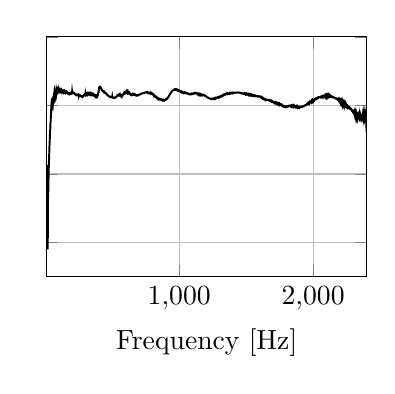
\begin{tikzpicture}

\begin{axis}[%
width=1.6in,
height=1.2in,
at={(1.011in,0.642in)},
scale only axis,
xmin=10,
xmax=2400,
xmajorgrids,
ymin=-30,
ymax=40,
ymajorgrids,
yticklabels={\empty},
xlabel={Frequency [Hz]},
axis background/.style={fill=white}
]
\addplot [color=black,line width=0.7pt,solid,forget plot]
  table[row sep=crcr]{%
0	-7.15873715654256\\
0.666675926054529	10.5087143459122\\
1.33335185210906	12.0967706112481\\
2.00002777816359	6.51246636920068\\
2.66670370421811	-0.175356461979414\\
3.33337963027264	-18.2069665387285\\
4.00005555632717	-15.6498849010992\\
4.6667314823817	-15.9720022096806\\
5.33340740843623	-12.3773277402846\\
6.00008333449076	-11.5127732534421\\
6.66675926054529	-13.124549272927\\
7.33343518659981	-16.8771871920024\\
8.00011111265434	-16.1609324436371\\
8.66678703870887	-16.3957874216142\\
9.3334629647634	-16.1414826002659\\
10.0001388908179	-9.11581854569876\\
10.6668148168725	2.63290680382195\\
11.333490742927	-1.30797727219537\\
12.0001666689815	-17.0636267744369\\
12.666842595036	-6.45026196358668\\
13.3335185210906	2.50663364486626\\
14.0001944471451	-1.70725075474316\\
14.6668703731996	-7.75658468652631\\
15.3335462992542	-9.3483774195719\\
16.0002222253087	-18.6218490262723\\
16.6668981513632	-9.45840899211946\\
17.3335740774177	-13.1140954030332\\
18.0002500034723	-21.9762082832002\\
18.6669259295268	-13.7328495691011\\
19.3336018555813	-11.8237285639594\\
20.0002777816359	-7.07261993440821\\
20.6669537076904	-6.4186096602619\\
21.3336296337449	-6.18112723880758\\
22.0003055597994	-3.42930466318585\\
22.666981485854	-5.04669005883661\\
23.3336574119085	-1.90200540857826\\
24.000333337963	-1.10164436043141\\
24.6670092640176	-0.272686762586023\\
25.3336851900721	1.2811352009495\\
26.0003611161266	2.57386832992159\\
26.6670370421811	2.79701323911136\\
27.3337129682357	3.92461706055076\\
28.0003888942902	4.5923075236652\\
28.6670648203447	5.33513322771373\\
29.3337407463993	6.22858231433341\\
30.0004166724538	6.93789285053402\\
30.6670925985083	7.88093877259057\\
31.3337685245628	8.5797174595324\\
32.0004444506174	9.13987555426015\\
32.6671203766719	9.69391198570301\\
33.3337963027264	10.471697172567\\
34.000472228781	11.2413498429474\\
34.6671481548355	11.9313674436524\\
35.33382408089	12.2206834471294\\
36.0005000069445	12.4355316665065\\
36.6671759329991	12.91188971702\\
37.3338518590536	13.6710847637875\\
38.0005277851081	14.5877480302561\\
38.6672037111627	15.0387885738662\\
39.3338796372172	15.0711002975034\\
40.0005555632717	15.2830740834027\\
40.6672314893262	16.2003603604853\\
41.3339074153808	16.9396542771061\\
42.0005833414353	17.2297836019304\\
42.6672592674898	17.5510274709084\\
43.3339351935444	18.3321890658326\\
44.0006111195989	19.0009998728534\\
44.6672870456534	19.3218972962387\\
45.3339629717079	19.7636726486508\\
46.0006388977625	20.5788804567535\\
46.667314823817	21.0659799329833\\
47.3339907498715	21.0706724489368\\
48.0006666759261	21.2954081888215\\
48.6673426019806	21.7504295307416\\
49.3340185280351	22.0226222784184\\
50.0006944540896	21.2851160722985\\
50.6673703801442	21.2051107463812\\
51.3340463061987	21.2927606988301\\
52.0007222322532	20.8577882479969\\
52.6673981583078	20.6711600742184\\
53.3340740843623	20.9203469279752\\
54.0007500104168	20.8221912113757\\
54.6674259364713	20.6991382976059\\
55.3341018625259	21.0407088483543\\
56.0007777885804	21.1298890830395\\
56.6674537146349	20.9530262480563\\
57.3341296406895	21.3766147555176\\
58.000805566744	21.5208537071508\\
58.6674814927985	21.2653058543976\\
59.334157418853	21.7307748662152\\
60.0008333449076	21.8951668040078\\
60.6675092709621	21.6512975974035\\
61.3341851970166	22.1294978753974\\
62.0008611230712	22.1845098242759\\
62.6675370491257	22.0945317033398\\
63.3342129751802	22.469571046389\\
64.0008889012347	22.4144126743392\\
64.6675648272893	22.4656633253754\\
65.3342407533438	22.7711307278621\\
66.0009166793983	22.595344049128\\
66.6675926054529	22.8211361901548\\
67.3342685315074	22.9714363429243\\
68.0009444575619	22.7483408524739\\
68.6676203836164	23.1900991734327\\
69.334296309671	23.0139565502041\\
70.0009722357255	23.0078941437368\\
70.66764816178	23.2640888008504\\
71.3343240878346	23.0521172453856\\
72.0010000138891	23.2968321488529\\
72.6676759399436	23.2063136781876\\
73.3343518659981	23.3339191542813\\
74.0010277920527	23.4201131005648\\
74.6677037181072	23.2737916065581\\
75.3343796441617	23.6255319273586\\
76.0010555702163	23.3345039510527\\
76.6677314962708	23.6224375724773\\
77.3344074223253	23.6114616424184\\
78.0010833483798	23.656576732508\\
78.6677592744344	23.7364151810855\\
79.3344352004889	23.7429745501262\\
80.0011111265434	23.8351365589793\\
80.667787052598	23.7447631942601\\
81.3344629786525	24.0074055842899\\
82.001138904707	23.8089022197667\\
82.6678148307615	24.0822291816178\\
83.3344907568161	23.9694717725242\\
84.0011666828706	24.1099258580291\\
84.6678426089251	24.0718306679598\\
85.3345185349797	24.2264814415983\\
86.0011944610342	24.1215006110483\\
86.6678703870887	24.2884169849204\\
87.3345463131432	24.2187384264903\\
88.0012222391978	24.3234554885306\\
88.6678981652523	24.3334222819882\\
89.3345740913068	24.3419120374625\\
90.0012500173614	24.3674475386358\\
90.6679259434159	24.4128618208234\\
91.3346018694704	24.3605904365201\\
92.0012777955249	24.490939092038\\
92.6679537215795	24.3883742537234\\
93.334629647634	24.5004186810227\\
94.0013055736885	24.4553094468998\\
94.667981499743	24.5035723715013\\
95.3346574257976	24.4446167778904\\
96.0013333518521	24.5316501403195\\
96.6680092779066	24.4406424070208\\
97.3346852039612	24.5138592854188\\
98.0013611300157	24.4334755790068\\
98.6680370560702	24.4430074171027\\
99.3347129821248	24.4448643874685\\
100.001388908179	24.5830026648291\\
100.668064834234	24.4380232462697\\
101.334740760288	24.367009642005\\
102.001416686343	24.4193073708642\\
102.668092612397	24.3062601108404\\
103.334768538452	24.3793294237293\\
104.001444464506	24.3564597657447\\
104.668120390561	24.3049224218097\\
105.334796316616	24.3674642786709\\
106.00147224267	24.2796963564791\\
106.668148168725	24.3472237616032\\
107.334824094779	24.3024466459277\\
108.001500020834	24.3293347604687\\
108.668175946888	24.3346573062107\\
109.334851872943	24.2937502414376\\
110.001527798997	24.3130074916196\\
110.668203725052	24.3272388220414\\
111.334879651106	24.3171147618053\\
112.001555577161	24.3363629515837\\
112.668231503215	24.3164517932769\\
113.33490742927	24.2788172766694\\
114.001583355324	24.353623658134\\
114.668259281379	24.2556978272775\\
115.334935207433	24.3056736662729\\
116.001611133488	24.2935033143821\\
116.668287059542	24.3115581567028\\
117.334962985597	24.2841837577282\\
118.001638911652	24.3345410688641\\
118.668314837706	24.2299614327879\\
119.334990763761	24.3242644212272\\
120.001666689815	24.2642435178612\\
120.66834261587	24.2865744746116\\
121.335018541924	24.2362265269981\\
122.001694467979	24.2878326149751\\
122.668370394033	24.199568432106\\
123.335046320088	24.2548448168798\\
124.001722246142	24.221737207819\\
124.668398172197	24.2279796362291\\
125.335074098251	24.1628143444844\\
126.001750024306	24.1726631684249\\
126.66842595036	24.1405365714659\\
127.335101876415	24.1014505663823\\
128.001777802469	24.1264812205878\\
128.668453728524	24.0820035236455\\
129.335129654579	24.0995864301708\\
130.001805580633	24.0159117359564\\
130.668481506688	24.0696150031467\\
131.335157432742	23.9974759426067\\
132.001833358797	24.0274658229844\\
132.668509284851	23.9846347041687\\
133.335185210906	24.0053856625507\\
134.00186113696	24.0257414417826\\
134.668537063015	23.9705604936007\\
135.335212989069	24.0116275950592\\
136.001888915124	23.9385430358016\\
136.668564841178	24.003448783508\\
137.335240767233	23.9357430250413\\
138.001916693287	23.9267099430717\\
138.668592619342	23.9397502148012\\
139.335268545396	23.9019035587597\\
140.001944471451	23.9667578531696\\
140.668620397506	23.9002705054755\\
141.33529632356	23.9301926792168\\
142.001972249615	23.9274379783929\\
142.668648175669	23.9107077654991\\
143.335324101724	23.9708240066973\\
144.002000027778	23.8976416979434\\
144.668675953833	23.9280605624893\\
145.335351879887	23.9395178290452\\
146.002027805942	23.9104477198023\\
146.668703731996	24.0042861899005\\
147.335379658051	23.9593716743793\\
148.002055584105	23.9548869966147\\
148.66873151016	23.9741124268126\\
149.335407436214	23.9137084328685\\
150.002083362269	24.0358334053608\\
150.668759288323	24.0129356581571\\
151.335435214378	23.9783044375457\\
152.002111140433	24.0135243729903\\
152.668787066487	23.9570176164768\\
153.335462992542	23.9373671861388\\
154.002138918596	24.0099718833998\\
154.668814844651	23.992175802195\\
155.335490770705	23.9905852435095\\
156.00216669676	24.0154380181123\\
156.668842622814	23.9448424581498\\
157.335518548869	23.9282342359544\\
158.002194474923	23.9412155054648\\
158.668870400978	23.8551568215683\\
159.335546327032	23.8452894749057\\
160.002222253087	23.881183650396\\
160.668898179141	23.8200251691604\\
161.335574105196	23.7885210433908\\
162.00225003125	23.8000977308225\\
162.668925957305	23.7368248711784\\
163.335601883359	23.6809154091656\\
164.002277809414	23.6665957710001\\
164.668953735469	23.6251820323242\\
165.335629661523	23.5786949380226\\
166.002305587578	23.5889468796819\\
166.668981513632	23.5848149862382\\
167.335657439687	23.5652098311667\\
168.002333365741	23.5511967971205\\
168.669009291796	23.5733584242023\\
169.33568521785	23.5538389244039\\
170.002361143905	23.5127478614158\\
170.669037069959	23.5456375024997\\
171.335712996014	23.537627613085\\
172.002388922068	23.4590023938168\\
172.669064848123	23.4686637651834\\
173.335740774177	23.4939816310679\\
174.002416700232	23.4211397740851\\
174.669092626286	23.3974198931325\\
175.335768552341	23.4132330294167\\
176.002444478396	23.4159270564024\\
176.66912040445	23.3919798536214\\
177.335796330505	23.3549185868886\\
178.002472256559	23.409420195141\\
178.669148182614	23.4296019615359\\
179.335824108668	23.3943393217074\\
180.002500034723	23.4064345494135\\
180.669175960777	23.4276710326754\\
181.335851886832	23.4763933629542\\
182.002527812886	23.4551022379621\\
182.669203738941	23.4466717248939\\
183.335879664995	23.4944683083156\\
184.00255559105	23.5051198154288\\
184.669231517104	23.521638340073\\
185.335907443159	23.4895152375784\\
186.002583369213	23.5116009885307\\
186.669259295268	23.5245887945761\\
187.335935221323	23.5634160727353\\
188.002611147377	23.5180171818616\\
188.669287073432	23.5007882491574\\
189.335962999486	23.4703268300687\\
190.002638925541	23.5218474907648\\
190.669314851595	23.5117957925876\\
191.33599077765	23.5073489030819\\
192.002666703704	23.4748867900627\\
192.669342629759	23.5238532127275\\
193.336018555813	23.5443500501714\\
194.002694481868	23.6052564056829\\
194.669370407922	23.6032195687775\\
195.336046333977	23.6067703614072\\
196.002722260031	23.6081462118097\\
196.669398186086	23.6284913263107\\
197.33607411214	23.6683757100492\\
198.002750038195	23.6500605877708\\
198.66942596425	23.6602688200448\\
199.336101890304	23.6430623940489\\
200.002777816359	23.9325844631997\\
200.669453742413	23.7295267431329\\
201.336129668468	23.7453272006813\\
202.002805594522	23.7956790146267\\
202.669481520577	23.7648214347693\\
203.336157446631	23.7392293326182\\
204.002833372686	23.732937791739\\
204.66950929874	23.7163043256602\\
205.336185224795	23.7762496457566\\
206.002861150849	23.8173995548699\\
206.669537076904	23.819690576325\\
207.336213002958	23.8133007788291\\
208.002888929013	23.7553494306647\\
208.669564855067	23.7263702197232\\
209.336240781122	23.7427961208167\\
210.002916707176	23.7457006858622\\
210.669592633231	23.7430014060931\\
211.336268559286	23.7336216256452\\
212.00294448534	23.690354867883\\
212.669620411395	23.664049586363\\
213.336296337449	23.6740149563915\\
214.002972263504	23.6470281106283\\
214.669648189558	23.5774503862567\\
215.336324115613	23.5200440720789\\
216.003000041667	23.501268482812\\
216.669675967722	23.4929198584724\\
217.336351893776	23.484777667757\\
218.003027819831	23.4627902735257\\
218.669703745885	23.4236067287961\\
219.33637967194	23.3896423123424\\
220.003055597994	23.3880062098513\\
220.669731524049	23.360435599666\\
221.336407450103	23.295373972138\\
222.003083376158	23.2435794936051\\
222.669759302213	23.2154136066346\\
223.336435228267	23.1782769365077\\
224.003111154322	23.1475453537114\\
224.669787080376	23.1410471008364\\
225.336463006431	23.1401937937074\\
226.003138932485	23.112688490254\\
226.66981485854	23.0846909271996\\
227.336490784594	23.1030816728332\\
228.003166710649	23.1383110228286\\
228.669842636703	23.0984731681706\\
229.336518562758	23.0754664321036\\
230.003194488812	23.1070024213092\\
230.669870414867	23.1393155792247\\
231.336546340921	23.1138425882487\\
232.003222266976	23.1025528200807\\
232.66989819303	23.0919111899043\\
233.336574119085	23.0269870112512\\
234.00325004514	22.9891308460617\\
234.669925971194	22.9989878077763\\
235.336601897249	23.0044408853645\\
236.003277823303	23.0079139293434\\
236.669953749358	23.053827118727\\
237.336629675412	23.0753116048292\\
238.003305601467	23.0506572130619\\
238.669981527521	23.0938313946732\\
239.336657453576	23.0801118803019\\
240.00333337963	23.0578906249399\\
240.670009305685	23.0979644782169\\
241.336685231739	23.0812668912868\\
242.003361157794	23.0627709669134\\
242.670037083848	23.098894118898\\
243.336713009903	23.0788132473687\\
244.003388935957	23.0869290004178\\
244.670064862012	23.1165807061338\\
245.336740788066	23.0898887826167\\
246.003416714121	23.1126726466507\\
246.670092640176	23.1194517032361\\
247.33676856623	23.0749178994239\\
248.003444492285	23.1072615007923\\
248.670120418339	23.0712759311162\\
249.336796344394	23.0631772802676\\
250.003472270448	22.8922414185675\\
250.670148196503	23.0048298809381\\
251.336824122557	23.0190106554729\\
252.003500048612	22.9874843352767\\
252.670175974666	22.9728118289677\\
253.336851900721	22.982477272407\\
254.003527826775	22.9583179686267\\
254.67020375283	22.9952054740954\\
255.336879678884	22.971121774093\\
256.003555604939	22.9865498886205\\
256.670231530993	22.9807406944549\\
257.336907457048	22.9681666605489\\
258.003583383103	22.9768272202065\\
258.670259309157	22.9192668609388\\
259.336935235212	22.9353555559673\\
260.003611161266	22.8702712699718\\
260.670287087321	22.8697452401716\\
261.336963013375	22.8121830398662\\
262.00363893943	22.81443725079\\
262.670314865484	22.7909267714697\\
263.336990791539	22.7905444968254\\
264.003666717593	22.7798958806609\\
264.670342643648	22.7740146447856\\
265.337018569702	22.7604926592849\\
266.003694495757	22.716614209319\\
266.670370421811	22.7021420662505\\
267.337046347866	22.6644170005054\\
268.00372227392	22.675102369387\\
268.670398199975	22.6585656693192\\
269.33707412603	22.6845816113223\\
270.003750052084	22.6737527254366\\
270.670425978139	22.6463608482636\\
271.337101904193	22.5953795718538\\
272.003777830248	22.5635895606184\\
272.670453756302	22.5674031766485\\
273.337129682357	22.5964060389313\\
274.003805608411	22.6309677360793\\
274.670481534466	22.6240231221093\\
275.33715746052	22.6236841124181\\
276.003833386575	22.5823719455308\\
276.670509312629	22.6111455283201\\
277.337185238684	22.5836961851879\\
278.003861164738	22.6328828994838\\
278.670537090793	22.6388029436635\\
279.337213016847	22.6636737409649\\
280.003888942902	22.6136392098819\\
280.670564868956	22.5802448996619\\
281.337240795011	22.6276271133216\\
282.003916721066	22.6693610695881\\
282.67059264712	22.7209756588301\\
283.337268573175	22.6859101869821\\
284.003944499229	22.7008570077434\\
284.670620425284	22.7234674390024\\
285.337296351338	22.7574004388151\\
286.003972277393	22.8445229709759\\
286.670648203447	22.8422932014905\\
287.337324129502	22.8336215459351\\
288.004000055556	22.8534736044996\\
288.670675981611	22.913823952474\\
289.337351907665	22.9758039708997\\
290.00402783372	22.9447318473799\\
290.670703759774	22.9535210499885\\
291.337379685829	22.9705623129775\\
292.004055611883	23.0256758850494\\
292.670731537938	23.0820633636433\\
293.337407463993	23.0286917736661\\
294.004083390047	23.027952961887\\
294.670759316102	23.1006304178873\\
295.337435242156	23.1056682211187\\
296.004111168211	23.1028400500452\\
296.670787094265	23.081667088508\\
297.33746302032	23.1088261705323\\
298.004138946374	23.1642148879404\\
298.670814872429	23.1531093623504\\
299.337490798483	23.1166864464385\\
300.004166724538	23.3665418070538\\
300.670842650592	23.2281860870225\\
301.337518576647	23.1662682127715\\
302.004194502701	23.1544402143831\\
302.670870428756	23.2342783454354\\
303.33754635481	23.2397236487141\\
304.004222280865	23.2038218162903\\
304.67089820692	23.207616142466\\
305.337574132974	23.2821001817681\\
306.004250059029	23.2330287871902\\
306.670925985083	23.2131033861347\\
307.337601911138	23.2352914154204\\
308.004277837192	23.2795248232929\\
308.670953763247	23.2099013595069\\
309.337629689301	23.2388779697744\\
310.004305615356	23.2800594659038\\
310.67098154141	23.2569280486767\\
311.337657467465	23.2114638342554\\
312.004333393519	23.299609424179\\
312.671009319574	23.2954833083898\\
313.337685245628	23.2558224068988\\
314.004361171683	23.2986141599806\\
314.671037097737	23.3661936285544\\
315.337713023792	23.312169742643\\
316.004388949847	23.3170811893786\\
316.671064875901	23.381741441126\\
317.337740801956	23.3355333422287\\
318.00441672801	23.3836132273774\\
318.671092654065	23.4126914826485\\
319.337768580119	23.3752190931115\\
320.004444506174	23.3986670195967\\
320.671120432228	23.4516374896275\\
321.337796358283	23.4144777344401\\
322.004472284337	23.3988945127971\\
322.671148210392	23.4423603982258\\
323.337824136446	23.4031282824876\\
324.004500062501	23.4396809699807\\
324.671175988555	23.4541101356225\\
325.33785191461	23.3771322764977\\
326.004527840664	23.4192964497452\\
326.671203766719	23.4264931341787\\
327.337879692774	23.3914217573799\\
328.004555618828	23.4557960765174\\
328.671231544883	23.4043099290427\\
329.337907470937	23.3937384344687\\
330.004583396992	23.4275941623696\\
330.671259323046	23.388045098902\\
331.337935249101	23.4432486139232\\
332.004611175155	23.4052667657364\\
332.67128710121	23.400573463867\\
333.337963027264	23.4401434219522\\
334.004638953319	23.357845359059\\
334.671314879373	23.4112267792951\\
335.337990805428	23.4006761429916\\
336.004666731482	23.3773302892184\\
336.671342657537	23.4304678684814\\
337.338018583591	23.3759822922548\\
338.004694509646	23.4198373123268\\
338.671370435701	23.3524395927385\\
339.338046361755	23.3533348287594\\
340.00472228781	23.3711708407037\\
340.671398213864	23.3132864465162\\
341.338074139919	23.3642997499883\\
342.004750065973	23.2957960291322\\
342.671425992028	23.3514068730671\\
343.338101918082	23.3257420257991\\
344.004777844137	23.3174921853021\\
344.671453770191	23.3031464955361\\
345.338129696246	23.263620991949\\
346.0048056223	23.3083246315707\\
346.671481548355	23.2417673165442\\
347.338157474409	23.2851718739417\\
348.004833400464	23.204452393028\\
348.671509326518	23.2326993738068\\
349.338185252573	23.1862953150634\\
350.004861178627	23.2024954774285\\
350.671537104682	23.2016188891564\\
351.338213030737	23.1974198598719\\
352.004888956791	23.1970438821182\\
352.671564882846	23.1711529885069\\
353.3382408089	23.2037763664283\\
354.004916734955	23.1677641995215\\
354.671592661009	23.2069921649515\\
355.338268587064	23.1650070213611\\
356.004944513118	23.1992209603012\\
356.671620439173	23.1409738539685\\
357.338296365227	23.1788912067377\\
358.004972291282	23.1027019847916\\
358.671648217336	23.1476111249839\\
359.338324143391	23.0786920764213\\
360.005000069445	23.1226919519339\\
360.6716759955	23.0611148901713\\
361.338351921554	23.092286326067\\
362.005027847609	23.0470916754452\\
362.671703773664	23.0664222074796\\
363.338379699718	23.0238804328784\\
364.005055625773	23.035169672148\\
364.671731551827	23.0093452500552\\
365.338407477882	22.9938314216959\\
366.005083403936	22.9830093396502\\
366.671759329991	22.950682957497\\
367.338435256045	22.9652681177984\\
368.0051111821	22.9115777998351\\
368.671787108154	22.9378777062769\\
369.338463034209	22.8725537469231\\
370.005138960263	22.9078087983924\\
370.671814886318	22.8444563514053\\
371.338490812372	22.8702265014038\\
372.005166738427	22.823562456798\\
372.671842664481	22.8208599571976\\
373.338518590536	22.8111223570435\\
374.005194516591	22.7522474525364\\
374.671870442645	22.7817476427405\\
375.3385463687	22.6941969850737\\
376.005222294754	22.7383231711478\\
376.671898220809	22.6754846835769\\
377.338574146863	22.6877581861511\\
378.005250072918	22.6906717089616\\
378.671925998972	22.658351924489\\
379.338601925027	22.705607335846\\
380.005277851081	22.6429832893611\\
380.671953777136	22.6691583584912\\
381.33862970319	22.6194392027024\\
382.005305629245	22.5757695192077\\
382.671981555299	22.5905242397834\\
383.338657481354	22.5197369972299\\
384.005333407408	22.5456802402232\\
384.672009333463	22.5340064505076\\
385.338685259517	22.5096147354606\\
386.005361185572	22.5682871856995\\
386.672037111627	22.5213255359728\\
387.338713037681	22.5711912354341\\
388.005388963736	22.625259679459\\
388.67206488979	22.6288198538351\\
389.338740815845	22.7603325712579\\
390.005416741899	22.8129192557627\\
390.672092667954	22.8784920405188\\
391.338768594008	23.0206437879727\\
392.005444520063	23.0769470015594\\
392.672120446117	23.2209934474768\\
393.338796372172	23.3752791549899\\
394.005472298226	23.4317600457901\\
394.672148224281	23.5820447454569\\
395.338824150335	23.7302811865809\\
396.00550007639	23.8240416597948\\
396.672176002444	24.0128021996323\\
397.338851928499	24.1482868134601\\
398.005527854554	24.2360199546688\\
398.672203780608	24.4474335771642\\
399.338879706663	24.6038826762412\\
400.005555632717	24.5605666726398\\
400.672231558772	24.8100488703285\\
401.338907484826	24.9634337837249\\
402.005583410881	25.0224017171142\\
402.672259336935	25.1189085776965\\
403.33893526299	25.235563413276\\
404.005611189044	25.2717036553352\\
404.672287115099	25.3314128075437\\
405.338963041153	25.3991343019002\\
406.005638967208	25.3935888823572\\
406.672314893262	25.3965680663757\\
407.338990819317	25.4356907615614\\
408.005666745371	25.4272133150631\\
408.672342671426	25.366634698988\\
409.339018597481	25.3729685396194\\
410.005694523535	25.3840453400317\\
410.67237044959	25.2965949046627\\
411.339046375644	25.2510525177916\\
412.005722301699	25.2758580500552\\
412.672398227753	25.2077616573045\\
413.339074153808	25.1164201027822\\
414.005750079862	25.1016445456299\\
414.672426005917	25.058259510491\\
415.339101931971	24.9882349890131\\
416.005777858026	24.9181123919607\\
416.67245378408	24.8757656863904\\
417.339129710135	24.8858751028074\\
418.005805636189	24.8112830993537\\
418.672481562244	24.7362554872007\\
419.339157488298	24.7263307536006\\
420.005833414353	24.7389744979165\\
420.672509340407	24.6800214622345\\
421.339185266462	24.5843610206647\\
422.005861192517	24.6022249994799\\
422.672537118571	24.5761496535907\\
423.339213044626	24.5646465042338\\
424.00588897068	24.4752897618484\\
424.672564896735	24.4285861432201\\
425.339240822789	24.4314731468244\\
426.005916748844	24.3979437025808\\
426.672592674898	24.3015094891424\\
427.339268600953	24.2545541748938\\
428.005944527007	24.2328455773834\\
428.672620453062	24.2737375769304\\
429.339296379116	24.2632491902619\\
430.005972305171	24.2057651955647\\
430.672648231225	24.1714503299811\\
431.33932415728	24.1623235443258\\
432.006000083334	24.1842873641646\\
432.672676009389	24.1828452161925\\
433.339351935444	24.1055814305408\\
434.006027861498	24.09285264821\\
434.672703787553	24.047628526424\\
435.339379713607	24.0911791492153\\
436.006055639662	24.0617381755948\\
436.672731565716	24.0487885524772\\
437.339407491771	23.9880694116177\\
438.006083417825	23.9276842342827\\
438.67275934388	23.9472251782106\\
439.339435269934	23.9199627050903\\
440.006111195989	23.9538873760375\\
440.672787122043	23.892317954538\\
441.339463048098	23.8535029673726\\
442.006138974152	23.813718178514\\
442.672814900207	23.7912046507748\\
443.339490826261	23.8011827237526\\
444.006166752316	23.8067842569663\\
444.672842678371	23.7821685741767\\
445.339518604425	23.7650070458023\\
446.00619453048	23.7125347109658\\
446.672870456534	23.6612109064161\\
447.339546382589	23.6582383057953\\
448.006222308643	23.6397043370453\\
448.672898234698	23.6398786909826\\
449.339574160752	23.6475041293184\\
450.006250086807	23.6220633837197\\
450.672926012861	23.5705148100686\\
451.339601938916	23.5441797931312\\
452.00627786497	23.4955456219766\\
452.672953791025	23.4503897931678\\
453.339629717079	23.4563352286849\\
454.006305643134	23.4331579273573\\
454.672981569188	23.425576157168\\
455.339657495243	23.4023542595\\
456.006333421298	23.4164633563494\\
456.673009347352	23.3596926012022\\
457.339685273407	23.329539130947\\
458.006361199461	23.282100168342\\
458.673037125516	23.2645172262514\\
459.33971305157	23.211896289963\\
460.006388977625	23.1642517273922\\
460.673064903679	23.1451054452469\\
461.339740829734	23.1215301660216\\
462.006416755788	23.1271164476067\\
462.673092681843	23.0785693515525\\
463.339768607897	23.0677163935001\\
464.006444533952	23.0535931639354\\
464.673120460006	23.0373979010306\\
465.339796386061	23.0214724946777\\
466.006472312115	22.9684360172689\\
466.67314823817	22.9492822646665\\
467.339824164225	22.9205703994463\\
468.006500090279	22.8892631135468\\
468.673176016334	22.8842417485463\\
469.339851942388	22.8362122012308\\
470.006527868443	22.8121458874946\\
470.673203794497	22.7881002412262\\
471.339879720552	22.7517999758853\\
472.006555646606	22.7575020839074\\
472.673231572661	22.7344592916752\\
473.339907498715	22.7201364600742\\
474.00658342477	22.7110151487217\\
474.673259350824	22.6790260133921\\
475.339935276879	22.6566296224347\\
476.006611202933	22.6398455086865\\
476.673287128988	22.6107385911572\\
477.339963055042	22.5921911313787\\
478.006638981097	22.5889108793928\\
478.673314907152	22.5665846391812\\
479.339990833206	22.5654983876713\\
480.006666759261	22.5764465071147\\
480.673342685315	22.5512033056028\\
481.34001861137	22.5359062912685\\
482.006694537424	22.5332557232302\\
482.673370463479	22.5096901998091\\
483.340046389533	22.4847600438032\\
484.006722315588	22.4827123785872\\
484.673398241642	22.4748141311656\\
485.340074167697	22.4535139679094\\
486.006750093751	22.4558405256336\\
486.673426019806	22.4576923512691\\
487.34010194586	22.4480277084016\\
488.006777871915	22.452118245327\\
488.673453797969	22.4723476677798\\
489.340129724024	22.4790314240742\\
490.006805650078	22.4701324928377\\
490.673481576133	22.4710256311865\\
491.340157502188	22.4746986008659\\
492.006833428242	22.458796802072\\
492.673509354297	22.436710203806\\
493.340185280351	22.4285228065914\\
494.006861206406	22.42974129422\\
494.67353713246	22.4146014883439\\
495.340213058515	22.3918596302885\\
496.006888984569	22.3873433462568\\
496.673564910624	22.4011294188386\\
497.340240836678	22.3993600031334\\
498.006916762733	22.3934189857785\\
498.673592688787	22.3959247581123\\
499.340268614842	22.3980804467826\\
500.006944540896	22.5556762884854\\
500.673620466951	22.3974492753894\\
501.340296393005	22.368857290977\\
502.00697231906	22.3462530764068\\
502.673648245115	22.3367616084347\\
503.340324171169	22.3236330454825\\
504.007000097224	22.3130497843336\\
504.673676023278	22.3087159923272\\
505.340351949333	22.3151007138196\\
506.007027875387	22.3309347341289\\
506.673703801442	22.3260035011254\\
507.340379727496	22.3026852159121\\
508.007055653551	22.2700563983849\\
508.673731579605	22.2289702448306\\
509.34040750566	22.227819946724\\
510.007083431714	22.2524631932524\\
510.673759357769	22.2852562256613\\
511.340435283823	22.2885169498584\\
512.007111209878	22.2530696843343\\
512.673787135932	22.2161262023443\\
513.340463061987	22.1976125470916\\
514.007138988041	22.222057758885\\
514.673814914096	22.2408173670611\\
515.340490840151	22.2532140444528\\
516.007166766205	22.255704132218\\
516.67384269226	22.2528469180602\\
517.340518618314	22.2412670775663\\
518.007194544369	22.2302604231504\\
518.673870470423	22.2580699907529\\
519.340546396478	22.2960580258133\\
520.007222322532	22.3215956694387\\
520.673898248587	22.292711184102\\
521.340574174641	22.2921542442947\\
522.007250100696	22.3191795064228\\
522.67392602675	22.3555140919138\\
523.340601952805	22.364265945962\\
524.007277878859	22.3797601749284\\
524.673953804914	22.3714415496905\\
525.340629730968	22.3680027167281\\
526.007305657023	22.4088621026103\\
526.673981583078	22.4640973821973\\
527.340657509132	22.4601723889253\\
528.007333435187	22.4487260807839\\
528.674009361241	22.4783243839663\\
529.340685287296	22.5159768553421\\
530.00736121335	22.5684477666636\\
530.674037139405	22.578746650228\\
531.340713065459	22.5672010872706\\
532.007388991514	22.613410184191\\
532.674064917568	22.6720092349587\\
533.340740843623	22.6848708485002\\
534.007416769677	22.7004009522696\\
534.674092695732	22.7033647144998\\
535.340768621786	22.7570213247332\\
536.007444547841	22.8066157979055\\
536.674120473896	22.7771235107182\\
537.34079639995	22.8103882371864\\
538.007472326005	22.8508287683496\\
538.674148252059	22.8809487827767\\
539.340824178114	22.8822835892378\\
540.007500104168	22.872836926273\\
540.674176030223	22.9409284225212\\
541.340851956277	22.9486301332984\\
542.007527882332	22.9503051462533\\
542.674203808386	22.9440067977203\\
543.340879734441	23.0121243840464\\
544.007555660495	23.0034512520761\\
544.67423158655	22.9891208696874\\
545.340907512604	23.010790639817\\
546.007583438659	23.0600250441806\\
546.674259364713	23.0299195345168\\
547.340935290768	23.0281484988089\\
548.007611216823	23.0740637133528\\
548.674287142877	23.076494011509\\
549.340963068932	23.0433162692488\\
550.007638994986	23.0889741013555\\
550.674314921041	23.1153192163153\\
551.340990847095	23.0904431790381\\
552.00766677315	23.0948912368854\\
552.674342699204	23.1411827306395\\
553.341018625259	23.0798824324349\\
554.007694551313	23.0976578046195\\
554.674370477368	23.1022173080237\\
555.341046403422	23.0775136151027\\
556.007722329477	23.0423404850017\\
556.674398255531	23.0845663505847\\
557.341074181586	23.0514846409615\\
558.00775010764	23.0222442900952\\
558.674426033695	23.0781988252938\\
559.341101959749	23.0016519343541\\
560.007777885804	22.9867363234617\\
560.674453811858	22.9995238939942\\
561.341129737913	22.9182260060531\\
562.007805663968	22.9071470208661\\
562.674481590022	22.8978954225745\\
563.341157516077	22.8276167423139\\
564.007833442131	22.8319379404363\\
564.674509368186	22.7980293203263\\
565.34118529424	22.7236366916712\\
566.007861220295	22.7328069820359\\
566.674537146349	22.6729735942675\\
567.341213072404	22.6476000823122\\
568.007888998458	22.6909341331093\\
568.674564924513	22.6183503679082\\
569.341240850567	22.6432736310698\\
570.007916776622	22.6595463287102\\
570.674592702676	22.6097747623807\\
571.341268628731	22.6929377403755\\
572.007944554785	22.7009934548951\\
572.67462048084	22.7021026774696\\
573.341296406895	22.7551728416182\\
574.007972332949	22.7505180240948\\
574.674648259004	22.8222548355523\\
575.341324185058	22.8412596694343\\
576.008000111113	22.8731501858362\\
576.674676037167	22.9496451050659\\
577.341351963222	22.9433182519649\\
578.008027889276	23.0342522269302\\
578.674703815331	23.0519341435632\\
579.341379741385	23.1121322335299\\
580.00805566744	23.1400469619068\\
580.674731593494	23.1552000982357\\
581.341407519549	23.2507566754524\\
582.008083445603	23.2489658838062\\
582.674759371658	23.3347560867854\\
583.341435297712	23.3344325894672\\
584.008111223767	23.4044509373415\\
584.674787149822	23.4331699427611\\
585.341463075876	23.4618953372666\\
586.008139001931	23.5328919450315\\
586.674814927985	23.5284988425091\\
587.34149085404	23.5757448014353\\
588.008166780094	23.5550104373674\\
588.674842706149	23.6571778406404\\
589.341518632203	23.6381512968117\\
590.008194558258	23.6965635088613\\
590.674870484312	23.6916376623203\\
591.341546410367	23.7451371180211\\
592.008222336421	23.7191740388327\\
592.674898262476	23.7718895764984\\
593.34157418853	23.8017976003933\\
594.008250114585	23.8229117895531\\
594.674926040639	23.8386868529616\\
595.341601966694	23.8782268859547\\
596.008277892749	23.8810183635803\\
596.674953818803	23.8756709635537\\
597.341629744858	23.9056998399092\\
598.008305670912	23.9031421113195\\
598.674981596967	23.9181515628447\\
599.341657523021	23.9508634240059\\
600.008333449076	23.8805873602388\\
600.67500937513	23.9622586843332\\
601.341685301185	23.9889985800693\\
602.008361227239	24.0026376782776\\
602.675037153294	23.9904799879627\\
603.341713079348	24.0386198925986\\
604.008389005403	23.9880625043385\\
604.675064931457	24.0611437363596\\
605.341740857512	24.0076429547272\\
606.008416783566	24.0519202565057\\
606.675092709621	24.0169048599477\\
607.341768635676	24.0588644656048\\
608.00844456173	24.0125309286435\\
608.675120487785	24.066765564531\\
609.341796413839	24.0119546403279\\
610.008472339894	24.0349107153302\\
610.675148265948	24.0239681379336\\
611.341824192003	23.9930567324848\\
612.008500118057	24.0367278043696\\
612.675176044112	23.9427825836015\\
613.341851970166	24.0136383106808\\
614.008527896221	23.9260728870395\\
614.675203822275	23.967874560845\\
615.34187974833	23.9386309128271\\
616.008555674384	23.9121841921643\\
616.675231600439	23.9527786815655\\
617.341907526493	23.8708946197959\\
618.008583452548	23.9409060531761\\
618.675259378603	23.869758995315\\
619.341935304657	23.8912419070363\\
620.008611230711	23.8831161386137\\
620.675287156766	23.8208071598346\\
621.341963082821	23.8456012404703\\
622.008639008875	23.7799195903703\\
622.67531493493	23.7539739552072\\
623.341990860984	23.7712922896337\\
624.008666787039	23.7059846392007\\
624.675342713093	23.736307461616\\
625.342018639148	23.7057318597623\\
626.008694565202	23.6457567355793\\
626.675370491257	23.6704860752896\\
627.342046417311	23.5846152449446\\
628.008722343366	23.5929820263484\\
628.67539826942	23.5927149191422\\
629.342074195475	23.534178373717\\
630.008750121529	23.5378234635832\\
630.675426047584	23.4899142794554\\
631.342101973638	23.4418013879416\\
632.008777899693	23.4648643283008\\
632.675453825748	23.4200253179656\\
633.342129751802	23.3738336644112\\
634.008805677857	23.3746893631768\\
634.675481603911	23.3017077656367\\
635.342157529966	23.3145078132275\\
636.00883345602	23.2782471960621\\
636.675509382075	23.2271912459278\\
637.342185308129	23.1865933222311\\
638.008861234184	23.2035485789039\\
638.675537160238	23.1457123345192\\
639.342213086293	23.1202529941746\\
640.008889012347	23.1266392408424\\
640.675564938402	23.0712377604073\\
641.342240864456	23.0985516195479\\
642.008916790511	23.0707215012686\\
642.675592716565	23.0583808867183\\
643.34226864262	23.0722746298861\\
644.008944568675	23.0757854678728\\
644.675620494729	23.0775737190015\\
645.342296420784	23.0655170251614\\
646.008972346838	23.1075933430503\\
646.675648272893	23.1032873247139\\
647.342324198947	23.0881326919386\\
648.009000125002	23.1283171868152\\
648.675676051056	23.1461635053042\\
649.342351977111	23.1451561411158\\
650.009027903165	23.1274044321186\\
650.67570382922	23.174074062497\\
651.342379755274	23.2165995015894\\
652.009055681329	23.1523605789994\\
652.675731607383	23.1796478983035\\
653.342407533438	23.2426741944987\\
654.009083459492	23.1942652917014\\
654.675759385547	23.1872648005046\\
655.342435311602	23.2039010623998\\
656.009111237656	23.2250070747326\\
656.675787163711	23.2131701195773\\
657.342463089765	23.1764770776587\\
658.00913901582	23.2067951136444\\
658.675814941874	23.2103111549554\\
659.342490867929	23.2263659548199\\
660.009166793983	23.1517168329694\\
660.675842720038	23.1637425728063\\
661.342518646092	23.2204451817756\\
662.009194572147	23.1850833790367\\
662.675870498201	23.1417722565883\\
663.342546424256	23.1340666490165\\
664.00922235031	23.1814717589597\\
664.675898276365	23.1479593637174\\
665.342574202419	23.1414817988859\\
666.009250128474	23.1011237830234\\
666.675926054529	23.1083220487726\\
667.342601980583	23.1116942065265\\
668.009277906638	23.1384149423654\\
668.675953832692	23.0763671735842\\
669.342629758747	23.0473479102096\\
670.009305684801	23.0466727826005\\
670.675981610856	23.1066009084499\\
671.34265753691	23.0605356569891\\
672.009333462965	23.0274246531842\\
672.676009389019	22.9986773913877\\
673.342685315074	23.0164546496092\\
674.009361241128	23.0306657792978\\
674.676037167183	23.015501261291\\
675.342713093237	23.0101616378404\\
676.009389019292	22.9644256087\\
676.676064945346	22.9727508843167\\
677.342740871401	22.9493790455104\\
678.009416797456	22.9720288308553\\
678.67609272351	22.9863316519141\\
679.342768649565	22.9663997270916\\
680.009444575619	22.9487900422614\\
680.676120501674	22.9024513546758\\
681.342796427728	22.9107880874405\\
682.009472353783	22.9512499995849\\
682.676148279837	22.9612981646361\\
683.342824205892	22.9696963441367\\
684.009500131946	22.9278079765716\\
684.676176058001	22.8881528900286\\
685.342851984055	22.9077360090166\\
686.00952791011	22.9132862841628\\
686.676203836164	22.9225816221733\\
687.342879762219	22.9567514469161\\
688.009555688273	22.939182938288\\
688.676231614328	22.9343930613014\\
689.342907540382	22.9485481762084\\
690.009583466437	22.9323852669615\\
690.676259392492	22.9236160133126\\
691.342935318546	22.9385515667977\\
692.009611244601	22.9460275375806\\
692.676287170655	22.9449960614785\\
693.34296309671	22.9775047277762\\
694.009639022764	23.0168108491432\\
694.676314948819	23.0147278233748\\
695.342990874873	23.0151084387104\\
696.009666800928	23.0314915693083\\
696.676342726982	23.0319153938354\\
697.343018653037	23.0092193284002\\
698.009694579091	23.0079175857448\\
698.676370505146	23.0389134326495\\
699.3430464312	23.0635381375235\\
700.009722357255	23.0806113725207\\
700.676398283309	23.1070747387522\\
701.343074209364	23.1429198483529\\
702.009750135419	23.1821318274822\\
702.676426061473	23.2034371400095\\
703.343101987528	23.1972361966381\\
704.009777913582	23.2023769448256\\
704.676453839637	23.2129795901655\\
705.343129765691	23.2377456291667\\
706.009805691746	23.2388210269578\\
706.6764816178	23.2402446979098\\
707.343157543855	23.2436202256167\\
708.009833469909	23.2531139776697\\
708.676509395964	23.2677796546635\\
709.343185322018	23.2950853772041\\
710.009861248073	23.3161448556964\\
710.676537174127	23.3230767972559\\
711.343213100182	23.3224069034599\\
712.009889026236	23.3363894122506\\
712.676564952291	23.352376178701\\
713.343240878346	23.3746584756115\\
714.0099168044	23.3897376175182\\
714.676592730455	23.4187604304551\\
715.343268656509	23.4314457069027\\
716.009944582564	23.4470768869404\\
716.676620508618	23.4473138841561\\
717.343296434673	23.4513154347126\\
718.009972360727	23.4618164961054\\
718.676648286782	23.4664520548425\\
719.343324212836	23.48092191548\\
720.010000138891	23.4868694976053\\
720.676676064945	23.4959092099804\\
721.343351991	23.5049851450233\\
722.010027917054	23.5152913741979\\
722.676703843109	23.5305386459897\\
723.343379769163	23.5348326469472\\
724.010055695218	23.5445654417811\\
724.676731621273	23.5504991007689\\
725.343407547327	23.5531631573508\\
726.010083473382	23.5690583822292\\
726.676759399436	23.5758723707306\\
727.343435325491	23.5926090661921\\
728.010111251545	23.6072628360651\\
728.6767871776	23.623601748347\\
729.343463103654	23.6329335257597\\
730.010139029709	23.6459222342708\\
730.676814955763	23.6525980284254\\
731.343490881818	23.6563295422292\\
732.010166807872	23.6524490742021\\
732.676842733927	23.647184839444\\
733.343518659981	23.633493465175\\
734.010194586036	23.622250891434\\
734.67687051209	23.6159784217895\\
735.343546438145	23.6190783694874\\
736.0102223642	23.6297958549446\\
736.676898290254	23.6526501551071\\
737.343574216309	23.6853001046733\\
738.010250142363	23.701724678475\\
738.676926068418	23.7203608777794\\
739.343601994472	23.7284602507321\\
740.010277920527	23.7187965816374\\
740.676953846581	23.7005295945607\\
741.343629772636	23.6926600441393\\
742.01030569869	23.6987851950776\\
742.676981624745	23.7149946195021\\
743.343657550799	23.7384591069874\\
744.010333476854	23.7561098397947\\
744.677009402908	23.7656183213648\\
745.343685328963	23.7724211810449\\
746.010361255017	23.7724226398048\\
746.677037181072	23.7798018559281\\
747.343713107127	23.7845976103599\\
748.010389033181	23.7807200609043\\
748.677064959236	23.7749101452311\\
749.34374088529	23.7741154810056\\
750.010416811345	23.796634395869\\
750.677092737399	23.8309667702415\\
751.343768663454	23.8433429958031\\
752.010444589508	23.8211403942757\\
752.677120515563	23.7865258034788\\
753.343796441617	23.7785537748694\\
754.010472367672	23.8137078229705\\
754.677148293726	23.8580048500374\\
755.343824219781	23.8458546378775\\
756.010500145835	23.8099426211288\\
756.67717607189	23.8030231652679\\
757.343851997944	23.8245262660432\\
758.010527923999	23.8210469904165\\
758.677203850054	23.8140119044577\\
759.343879776108	23.8294331705672\\
760.010555702162	23.8467926262879\\
760.677231628217	23.8025592074172\\
761.343907554272	23.7703411426533\\
762.010583480326	23.8015819343721\\
762.677259406381	23.8354867147965\\
763.343935332435	23.8077505483757\\
764.01061125849	23.7721403159768\\
764.677287184544	23.7745036805367\\
765.343963110599	23.7911545262541\\
766.010639036653	23.8057779241814\\
766.677314962708	23.7873733000585\\
767.343990888762	23.7461609218968\\
768.010666814817	23.753132996585\\
768.677342740871	23.7736846193395\\
769.344018666926	23.7601698551631\\
770.01069459298	23.7618074665837\\
770.677370519035	23.7302630308509\\
771.344046445089	23.7042278043597\\
772.010722371144	23.7574223447078\\
772.677398297199	23.7487646456219\\
773.344074223253	23.6839789911615\\
774.010750149308	23.7089975063742\\
774.677426075362	23.7273710275949\\
775.344102001417	23.7155070618461\\
776.010777927471	23.6884144581687\\
776.677453853526	23.6816103531152\\
777.34412977958	23.707294241114\\
778.010805705635	23.6926215517277\\
778.677481631689	23.6866564038993\\
779.344157557744	23.6474536777702\\
780.010833483798	23.6946382443034\\
780.677509409853	23.6978930964141\\
781.344185335907	23.6335629969068\\
782.010861261962	23.6634253692965\\
782.677537188016	23.6684351830178\\
783.344213114071	23.6543849525892\\
784.010889040126	23.6321139751109\\
784.67756496618	23.6586669126238\\
785.344240892235	23.6377648414625\\
786.010916818289	23.6430628515877\\
786.677592744344	23.5962724813471\\
787.344268670398	23.6591462122314\\
788.010944596453	23.5986072018452\\
788.677620522507	23.5932668974924\\
789.344296448562	23.6056921710213\\
790.010972374616	23.594592645914\\
790.677648300671	23.5589758714033\\
791.344324226725	23.578499149603\\
792.01100015278	23.5619152783938\\
792.677676078834	23.5371886993653\\
793.344352004889	23.5175638743205\\
794.011027930943	23.5410699929958\\
794.677703856998	23.4847255499225\\
795.344379783053	23.4762598301396\\
796.011055709107	23.5007746126234\\
796.677731635162	23.4334251169915\\
797.344407561216	23.4406835334558\\
798.011083487271	23.423551780872\\
798.677759413325	23.3836615258482\\
799.34443533938	23.3712116964328\\
800.011111265434	23.3464470775564\\
800.677787191489	23.3123855994777\\
801.344463117543	23.330251517603\\
802.011139043598	23.2740297828944\\
802.677814969652	23.2650722911698\\
803.344490895707	23.232593118773\\
804.011166821761	23.2270389770053\\
804.677842747816	23.1822096779909\\
805.34451867387	23.1771461965789\\
806.011194599925	23.1282878184583\\
806.67787052598	23.1238834650183\\
807.344546452034	23.0902544246641\\
808.011222378089	23.0570561101117\\
808.677898304143	23.0466976640198\\
809.344574230198	23.0298038025368\\
810.011250156252	22.9588441094959\\
810.677926082307	23.0018697553262\\
811.344602008361	22.936597138072\\
812.011277934416	22.9259417004265\\
812.67795386047	22.9100470182289\\
813.344629786525	22.8835386128617\\
814.011305712579	22.8558248487175\\
814.677981638634	22.833480860987\\
815.344657564688	22.8180939307043\\
816.011333490743	22.8135784254726\\
816.678009416797	22.7463410111136\\
817.344685342852	22.7610203829671\\
818.011361268907	22.7322922194165\\
818.678037194961	22.7188892031191\\
819.344713121016	22.7025841491073\\
820.01138904707	22.6442547833458\\
820.678064973125	22.6752305102308\\
821.344740899179	22.6301203342746\\
822.011416825234	22.6346224297041\\
822.678092751288	22.5772283453905\\
823.344768677343	22.5661822918427\\
824.011444603397	22.5605695533062\\
824.678120529452	22.5439826769726\\
825.344796455506	22.5184558752568\\
826.011472381561	22.4916776544438\\
826.678148307615	22.4661267185983\\
827.34482423367	22.4357930121631\\
828.011500159724	22.4503824207671\\
828.678176085779	22.397339954099\\
829.344852011833	22.4158834114791\\
830.011527937888	22.3319052618051\\
830.678203863943	22.3448836532995\\
831.344879789997	22.2925004629504\\
832.011555716052	22.2871201245659\\
832.678231642106	22.254574550138\\
833.344907568161	22.2678164347568\\
834.011583494215	22.2094249817561\\
834.67825942027	22.2209623225987\\
835.344935346324	22.1716725844095\\
836.011611272379	22.1579734071428\\
836.678287198433	22.1250104460861\\
837.344963124488	22.1162106211392\\
838.011639050542	22.0759210373798\\
838.678314976597	22.0920289821163\\
839.344990902651	22.0415325424152\\
840.011666828706	22.0379083196923\\
840.67834275476	22.0126529796581\\
841.345018680815	22.0354222971823\\
842.01169460687	21.9657744513101\\
842.678370532924	21.9950627024183\\
843.345046458979	21.959362056018\\
844.011722385033	21.9539106245945\\
844.678398311088	21.9127198983184\\
845.345074237142	21.9525727640256\\
846.011750163197	21.909164958997\\
846.678426089251	21.8993191942726\\
847.345102015306	21.8932463793399\\
848.01177794136	21.886800682874\\
848.678453867415	21.8777113216721\\
849.345129793469	21.8454854133775\\
850.011805719524	21.8744706843142\\
850.678481645578	21.8400531616394\\
851.345157571633	21.8574032707273\\
852.011833497687	21.8063399602622\\
852.678509423742	21.8291707988836\\
853.345185349797	21.8257764326659\\
854.011861275851	21.7920142319313\\
854.678537201906	21.7928114019926\\
855.34521312796	21.7752680482553\\
856.011889054015	21.8102587561136\\
856.678564980069	21.7767600698792\\
857.345240906124	21.7843125355645\\
858.011916832178	21.7897629958131\\
858.678592758233	21.781905592999\\
859.345268684287	21.8035182433575\\
860.011944610342	21.7503954752272\\
860.678620536396	21.7480540067359\\
861.345296462451	21.7415960650876\\
862.011972388505	21.7212121050725\\
862.67864831456	21.749083622938\\
863.345324240614	21.7141188451205\\
864.012000166669	21.7202243529592\\
864.678676092724	21.7154410623752\\
865.345352018778	21.6783093078939\\
866.012027944833	21.7017993120571\\
866.678703870887	21.6723481207449\\
867.345379796942	21.6566507884827\\
868.012055722996	21.6795393051187\\
868.678731649051	21.6347461431731\\
869.345407575105	21.6315565589786\\
870.01208350116	21.6392495452065\\
870.678759427214	21.614280067601\\
871.345435353269	21.6464405978681\\
872.012111279323	21.6237430638077\\
872.678787205378	21.5647319128906\\
873.345463131432	21.5826831368792\\
874.012139057487	21.5882032792836\\
874.678814983541	21.5773477270498\\
875.345490909596	21.593680803421\\
876.012166835651	21.563401697428\\
876.678842761705	21.5531643714124\\
877.34551868776	21.5765163789445\\
878.012194613814	21.5545320706207\\
878.678870539869	21.508288417968\\
879.345546465923	21.5498812009246\\
880.012222391978	21.5508132863589\\
880.678898318032	21.5147545437381\\
881.345574244087	21.5404085172841\\
882.012250170141	21.5761681482087\\
882.678926096196	21.5328328401813\\
883.34560202225	21.5403201255586\\
884.012277948305	21.5774516174571\\
884.678953874359	21.5446492409024\\
885.345629800414	21.5214067170058\\
886.012305726468	21.568381277268\\
886.678981652523	21.5582926654186\\
887.345657578578	21.5245749775924\\
888.012333504632	21.5687494403617\\
888.679009430687	21.5763740500678\\
889.345685356741	21.5445564244656\\
890.012361282796	21.5770259220888\\
890.67903720885	21.5924344238192\\
891.345713134905	21.591049981083\\
892.012389060959	21.5847696890082\\
892.679064987014	21.5914002202303\\
893.345740913068	21.6267422328808\\
894.012416839123	21.6236499848409\\
894.679092765177	21.6103529758651\\
895.345768691232	21.6457718459671\\
896.012444617286	21.6602353657822\\
896.679120543341	21.6617842155454\\
897.345796469395	21.6532574688718\\
898.01247239545	21.6770009716539\\
898.679148321504	21.7234366548891\\
899.345824247559	21.7010498376848\\
900.012500173613	21.6935042041642\\
900.679176099668	21.7212166697007\\
901.345852025723	21.7760315091477\\
902.012527951777	21.7748452027565\\
902.679203877832	21.7817350053831\\
903.345879803886	21.7924738048583\\
904.012555729941	21.8348492709104\\
904.679231655995	21.8564750859\\
905.34590758205	21.8660910496602\\
906.012583508104	21.8705077703193\\
906.679259434159	21.9037522513475\\
907.345935360213	21.9494467052829\\
908.012611286268	21.9928283132141\\
908.679287212322	21.9975600231928\\
909.345963138377	22.0191063476531\\
910.012639064431	22.0456857305327\\
910.679314990486	22.1016801456314\\
911.34599091654	22.1173822053652\\
912.012666842595	22.1445521461763\\
912.67934276865	22.1347443194722\\
913.346018694704	22.1858045676258\\
914.012694620759	22.2101527156677\\
914.679370546813	22.2751835198286\\
915.346046472868	22.3193304201988\\
916.012722398922	22.3327929131323\\
916.679398324977	22.3850078651014\\
917.346074251031	22.3897869317004\\
918.012750177086	22.4600814758659\\
918.67942610314	22.4925894131589\\
919.346102029195	22.5234268441138\\
920.012777955249	22.5698865144314\\
920.679453881304	22.5924000490605\\
921.346129807358	22.6526245511415\\
922.012805733413	22.7088826307128\\
922.679481659467	22.7417421025648\\
923.346157585522	22.802833481229\\
924.012833511577	22.8242587839818\\
924.679509437631	22.8643774587498\\
925.346185363686	22.9206038729767\\
926.01286128974	22.9552323534503\\
926.679537215795	22.9909762710224\\
927.346213141849	23.0582506070459\\
928.012889067904	23.0944683718885\\
928.679564993958	23.142439532014\\
929.346240920013	23.2099693424213\\
930.012916846067	23.2491488401517\\
930.679592772122	23.2576291675653\\
931.346268698176	23.2979576862761\\
932.012944624231	23.3431067554339\\
932.679620550285	23.3856348281568\\
933.34629647634	23.4484277106392\\
934.012972402394	23.5031449956164\\
934.679648328449	23.5308505186907\\
935.346324254504	23.5652804033016\\
936.013000180558	23.6332746499125\\
936.679676106613	23.6804375262843\\
937.346352032667	23.6905779861082\\
938.013027958722	23.7024347967036\\
938.679703884776	23.7570073631558\\
939.346379810831	23.8117806859368\\
940.013055736885	23.8302794714931\\
940.67973166294	23.8497056363086\\
941.346407588994	23.8957754099035\\
942.013083515049	23.9516303796942\\
942.679759441103	23.9950593671841\\
943.346435367158	24.0254469090188\\
944.013111293212	24.0575536157964\\
944.679787219267	24.0933925833592\\
945.346463145321	24.1176567602279\\
946.013139071376	24.1543954100307\\
946.679814997431	24.2105260217861\\
947.346490923485	24.2266489199503\\
948.01316684954	24.2200349629342\\
948.679842775594	24.2495478492496\\
949.346518701649	24.2857147321641\\
950.013194627703	24.2975242154483\\
950.679870553758	24.333740230934\\
951.346546479812	24.3739990029084\\
952.013222405867	24.3750952835269\\
952.679898331921	24.3806588785275\\
953.346574257976	24.4059096046819\\
954.01325018403	24.4160637253644\\
954.679926110085	24.4175874974566\\
955.346602036139	24.4538675256407\\
956.013277962194	24.4767718043389\\
956.679953888248	24.4755922960887\\
957.346629814303	24.515576177942\\
958.013305740358	24.5350638853597\\
958.679981666412	24.5301349632723\\
959.346657592467	24.5649936050012\\
960.013333518521	24.5675572993424\\
960.680009444576	24.5651371503972\\
961.34668537063	24.5962704976339\\
962.013361296685	24.5847714533879\\
962.680037222739	24.5949610237168\\
963.346713148794	24.6199034368168\\
964.013389074848	24.6069113793909\\
964.680065000903	24.634519299941\\
965.346740926957	24.6390409042201\\
966.013416853012	24.625447257267\\
966.680092779066	24.6586466670165\\
967.346768705121	24.63011606311\\
968.013444631175	24.6523727541653\\
968.68012055723	24.6491347442191\\
969.346796483284	24.6323060450059\\
970.013472409339	24.6531270390028\\
970.680148335394	24.6281686635377\\
971.346824261448	24.6469585719813\\
972.013500187503	24.6410670451603\\
972.680176113557	24.6384469996364\\
973.346852039612	24.660786427938\\
974.013527965666	24.6428409564762\\
974.680203891721	24.6744709051982\\
975.346879817775	24.6427568025011\\
976.01355574383	24.6658855791044\\
976.680231669884	24.6358628244052\\
977.346907595939	24.627487151939\\
978.013583521993	24.6173274996003\\
978.680259448048	24.60330763951\\
979.346935374102	24.6087240743825\\
980.013611300157	24.5915353157645\\
980.680287226211	24.6184640058517\\
981.346963152266	24.5908009431497\\
982.013639078321	24.6147904663397\\
982.680315004375	24.5820328187724\\
983.34699093043	24.5949808720948\\
984.013666856484	24.5524231793613\\
984.680342782539	24.5747220550406\\
985.347018708593	24.5374480356849\\
986.013694634648	24.5451236033216\\
986.680370560702	24.5059062889597\\
987.347046486757	24.525211286787\\
988.013722412811	24.5143745919227\\
988.680398338866	24.5395278027253\\
989.34707426492	24.4908220149564\\
990.013750190975	24.4815587430205\\
990.680426117029	24.4268379860158\\
991.347102043084	24.4489158755179\\
992.013777969138	24.4436657672341\\
992.680453895193	24.4523353493046\\
993.347129821248	24.4170978745725\\
994.013805747302	24.3911807738439\\
994.680481673357	24.3768679385913\\
995.347157599411	24.355733594557\\
996.013833525466	24.3594851732301\\
996.68050945152	24.3282866883676\\
997.347185377575	24.3583537443951\\
998.013861303629	24.3116783037083\\
998.680537229684	24.280515357315\\
999.347213155738	24.2569248426329\\
1000.01388908179	24.2609980864803\\
1000.68056500785	24.2797312127906\\
1001.3472409339	24.217642945276\\
1002.01391685996	24.2257912097319\\
1002.68059278601	24.1968321968516\\
1003.34726871207	24.1799417367418\\
1004.01394463812	24.1919735095043\\
1004.68062056417	24.1699420575306\\
1005.34729649023	24.1376761696946\\
1006.01397241628	24.108605247232\\
1006.68064834234	24.1297446113012\\
1007.34732426839	24.1217339763472\\
1008.01400019445	24.0757545064011\\
1008.6806761205	24.0741660074906\\
1009.34735204656	24.0432140624618\\
1010.01402797261	24.0492385601251\\
1010.68070389867	24.0617936184925\\
1011.34737982472	23.9974552886562\\
1012.01405575077	23.9988267395006\\
1012.68073167683	24.0078679724104\\
1013.34740760288	23.9894511080756\\
1014.01408352894	23.9719791427796\\
1014.68075945499	23.9385598987956\\
1015.34743538105	23.9490635946811\\
1016.0141113071	23.9415833165908\\
1016.68078723316	23.9336876011183\\
1017.34746315921	23.898928508809\\
1018.01413908527	23.899767753983\\
1018.68081501132	23.9318471726578\\
1019.34749093737	23.8618397982304\\
1020.01416686343	23.8725155805608\\
1020.68084278948	23.8820160242071\\
1021.34751871554	23.8815575250043\\
1022.01419464159	23.8264402090162\\
1022.68087056765	23.8568310100061\\
1023.3475464937	23.8655164232773\\
1024.01422241976	23.8273396966205\\
1024.68089834581	23.8209805063739\\
1025.34757427186	23.8533391441952\\
1026.01425019792	23.8344813434616\\
1026.68092612397	23.8046729464469\\
1027.34760205003	23.8235807759358\\
1028.01427797608	23.8430100511142\\
1028.68095390214	23.8006006907619\\
1029.34762982819	23.8020720525931\\
1030.01430575425	23.8270987303741\\
1030.6809816803	23.8291174860634\\
1031.34765760636	23.7730953884581\\
1032.01433353241	23.8112488196693\\
1032.68100945846	23.8017842072972\\
1033.34768538452	23.813243786809\\
1034.01436131057	23.7991354117519\\
1034.68103723663	23.7957721784816\\
1035.34771316268	23.7985364278811\\
1036.01438908874	23.8104739520658\\
1036.68106501479	23.8197767183482\\
1037.34774094085	23.7672552170649\\
1038.0144168669	23.8005108365336\\
1038.68109279296	23.8105887546465\\
1039.34776871901	23.7882191127178\\
1040.01444464506	23.8117792449911\\
1040.68112057112	23.7723055198566\\
1041.34779649717	23.7729295529168\\
1042.01447242323	23.8062689660195\\
1042.68114834928	23.7768180603605\\
1043.34782427534	23.7838240220809\\
1044.01450020139	23.7718375180664\\
1044.68117612745	23.7298847441733\\
1045.3478520535	23.7614699139402\\
1046.01452797956	23.768881358182\\
1046.68120390561	23.7325348161235\\
1047.34787983166	23.749383185132\\
1048.01455575772	23.7239645230732\\
1048.68123168377	23.6878749326431\\
1049.34790760983	23.7073345859676\\
1050.01458353588	23.7048962220219\\
1050.68125946194	23.6936632373815\\
1051.34793538799	23.6880258497942\\
1052.01461131405	23.6755006298913\\
1052.6812872401	23.6575894244404\\
1053.34796316616	23.6099380093988\\
1054.01463909221	23.6214380343394\\
1054.68131501826	23.6265221712357\\
1055.34799094432	23.607211159936\\
1056.01466687037	23.594997072534\\
1056.68134279643	23.5883276922451\\
1057.34801872248	23.5947522933886\\
1058.01469464854	23.5543844817275\\
1058.68137057459	23.5266734600883\\
1059.34804650065	23.5196418783692\\
1060.0147224267	23.5132393528225\\
1060.68139835275	23.5202321561894\\
1061.34807427881	23.4776635143966\\
1062.01475020486	23.4870583418948\\
1062.68142613092	23.4763627870469\\
1063.34810205697	23.4918960677406\\
1064.01477798303	23.4800213745195\\
1064.68145390908	23.4562914678957\\
1065.34812983514	23.4417191776805\\
1066.01480576119	23.4191075288817\\
1066.68148168725	23.4358371456784\\
1067.3481576133	23.4124470154536\\
1068.01483353935	23.4224716939945\\
1068.68150946541	23.3802523945705\\
1069.34818539146	23.3821364174618\\
1070.01486131752	23.3451022068856\\
1070.68153724357	23.3574050358997\\
1071.34821316963	23.3428690784554\\
1072.01488909568	23.3592725946215\\
1072.68156502174	23.3418444029471\\
1073.34824094779	23.3460159075539\\
1074.01491687385	23.3249070730927\\
1074.6815927999	23.3272417845061\\
1075.34826872595	23.3009734999618\\
1076.01494465201	23.3043560847974\\
1076.68162057806	23.2870161501102\\
1077.34829650412	23.2911689537725\\
1078.01497243017	23.2795098958665\\
1078.68164835623	23.2990866593878\\
1079.34832428228	23.2787837715382\\
1080.01500020834	23.3046712475635\\
1080.68167613439	23.2884720168787\\
1081.34835206045	23.3108545771808\\
1082.0150279865	23.2881430531773\\
1082.68170391255	23.3173930591884\\
1083.34837983861	23.2999858066857\\
1084.01505576466	23.324721974604\\
1084.68173169072	23.3114050940252\\
1085.34840761677	23.3305460200536\\
1086.01508354283	23.3261098445586\\
1086.68175946888	23.3335818577664\\
1087.34843539494	23.339058895783\\
1088.01511132099	23.3239688613141\\
1088.68178724705	23.3452588975995\\
1089.3484631731	23.3088869314408\\
1090.01513909915	23.3345065851815\\
1090.68181502521	23.3089646595555\\
1091.34849095126	23.3246147360154\\
1092.01516687732	23.3123833110667\\
1092.68184280337	23.3231706112779\\
1093.34851872943	23.3443269769584\\
1094.01519465548	23.3363070509737\\
1094.68187058154	23.3758363494172\\
1095.34854650759	23.3504421465917\\
1096.01522243365	23.3689343398928\\
1096.6818983597	23.372791138772\\
1097.34857428575	23.3708758949561\\
1098.01525021181	23.3999768580514\\
1098.68192613786	23.3866844475672\\
1099.34860206392	23.4178339625415\\
1100.01527798997	23.4087912737511\\
1100.68195391603	23.4018945135339\\
1101.34862984208	23.4210448259752\\
1102.01530576814	23.4061288341679\\
1102.68198169419	23.438545221447\\
1103.34865762024	23.4640627394402\\
1104.0153335463	23.4559936410174\\
1104.68200947235	23.4814513738994\\
1105.34868539841	23.450489783193\\
1106.01536132446	23.4485884152519\\
1106.68203725052	23.4916026321279\\
1107.34871317657	23.4922995621585\\
1108.01538910263	23.5225751759419\\
1108.68206502868	23.5171955342749\\
1109.34874095474	23.4903689871799\\
1110.01541688079	23.5244734530082\\
1110.68209280684	23.5373205764666\\
1111.3487687329	23.5391760066027\\
1112.01544465895	23.5566124382849\\
1112.68212058501	23.5381588486082\\
1113.34879651106	23.5428733309569\\
1114.01547243712	23.5838510169222\\
1114.68214836317	23.5695669738166\\
1115.34882428923	23.5680698244739\\
1116.01550021528	23.5939607153734\\
1116.68217614134	23.5779315946213\\
1117.34885206739	23.5715105046879\\
1118.01552799344	23.6123068849756\\
1118.6822039195	23.6047602094315\\
1119.34887984555	23.5780308729956\\
1120.01555577161	23.5984720326085\\
1120.68223169766	23.6259545987134\\
1121.34890762372	23.5995277729751\\
1122.01558354977	23.5898457922455\\
1122.68225947583	23.6157337264921\\
1123.34893540188	23.6226431726956\\
1124.01561132794	23.5916230859616\\
1124.68228725399	23.6039846392657\\
1125.34896318004	23.6186873444267\\
1126.0156391061	23.5888779294176\\
1126.68231503215	23.5780040557504\\
1127.34899095821	23.6081326542277\\
1128.01566688426	23.5741338469113\\
1128.68234281032	23.560935161589\\
1129.34901873637	23.583506118574\\
1130.01569466243	23.5573464656565\\
1130.68237058848	23.5461278224982\\
1131.34904651453	23.5372265088965\\
1132.01572244059	23.5425264792661\\
1132.68239836664	23.5346780111683\\
1133.3490742927	23.4786094694783\\
1134.01575021875	23.5189742911937\\
1134.68242614481	23.5096522888697\\
1135.34910207086	23.4458488198633\\
1136.01577799692	23.4696726203743\\
1136.68245392297	23.4556412887498\\
1137.34912984903	23.4465170273563\\
1138.01580577508	23.4262386999326\\
1138.68248170113	23.4055411253135\\
1139.34915762719	23.3850141856985\\
1140.01583355324	23.4035505682626\\
1140.6825094793	23.3800131544329\\
1141.34918540535	23.3212522906109\\
1142.01586133141	23.3597766001778\\
1142.68253725746	23.3120153363747\\
1143.34921318352	23.3366669385656\\
1144.01588910957	23.2877474685884\\
1144.68256503563	23.271357012179\\
1145.34924096168	23.2721834693364\\
1146.01591688773	23.2786492989679\\
1146.68259281379	23.2345005924128\\
1147.34926873984	23.2518388607174\\
1148.0159446659	23.1846887655732\\
1148.68262059195	23.2370588546912\\
1149.34929651801	23.1916425403293\\
1150.01597244406	23.2051681515907\\
1150.68264837012	23.1797530775029\\
1151.34932429617	23.1467641416644\\
1152.01600022223	23.1706095617247\\
1152.68267614828	23.1371290047396\\
1153.34935207433	23.1735331885055\\
1154.01602800039	23.1182724256666\\
1154.68270392644	23.1340448244712\\
1155.3493798525	23.1088599989435\\
1156.01605577855	23.1063349104935\\
1156.68273170461	23.1297039066936\\
1157.34940763066	23.0853417008309\\
1158.01608355672	23.1308369920891\\
1158.68275948277	23.064297969931\\
1159.34943540883	23.0921739215049\\
1160.01611133488	23.0736539933081\\
1160.68278726093	23.0794602492005\\
1161.34946318699	23.0828375910094\\
1162.01613911304	23.0869997913755\\
1162.6828150391	23.0529207676691\\
1163.34949096515	23.0810282240626\\
1164.01616689121	23.0515068894226\\
1164.68284281726	23.0547431297087\\
1165.34951874332	23.0725201641835\\
1166.01619466937	23.0641881451531\\
1166.68287059542	23.0507460905254\\
1167.34954652148	23.0871242078753\\
1168.01622244753	23.0480366447754\\
1168.68289837359	23.046827607419\\
1169.34957429964	23.0477898557065\\
1170.0162502257	23.0687341631493\\
1170.68292615175	23.0279806158983\\
1171.34960207781	23.0697463754378\\
1172.01627800386	23.0645252256015\\
1172.68295392992	23.0731660805469\\
1173.34962985597	23.0386573725005\\
1174.01630578202	23.0766952449275\\
1174.68298170808	23.0732348815066\\
1175.34965763413	23.0583185651438\\
1176.01633356019	23.0507569724877\\
1176.68300948624	23.051584829486\\
1177.3496854123	23.0790167690067\\
1178.01636133835	23.0373102794049\\
1178.68303726441	23.0511951612413\\
1179.34971319046	23.0407652347095\\
1180.01638911652	23.0663366054357\\
1180.68306504257	23.0626200875565\\
1181.34974096862	23.0309988171098\\
1182.01641689468	23.0398208133504\\
1182.68309282073	23.0284212811989\\
1183.34976874679	23.0474669082934\\
1184.01644467284	23.0337156263395\\
1184.6831205989	22.9989362764271\\
1185.34979652495	22.9965347249001\\
1186.01647245101	22.9692066782078\\
1186.68314837706	22.9791760997082\\
1187.34982430312	22.9794432406585\\
1188.01650022917	22.9511550891924\\
1188.68317615522	22.948565592521\\
1189.34985208128	22.9138048776704\\
1190.01652800733	22.8838945536479\\
1190.68320393339	22.8938782327377\\
1191.34987985944	22.8624336707805\\
1192.0165557855	22.8601938767356\\
1192.68323171155	22.8631551532058\\
1193.34990763761	22.8274955838589\\
1194.01658356366	22.8248290050367\\
1194.68325948972	22.8076769231163\\
1195.34993541577	22.769271191237\\
1196.01661134182	22.7502728708399\\
1196.68328726788	22.7464469423278\\
1197.34996319393	22.6968071762329\\
1198.01663911999	22.6934994142325\\
1198.68331504604	22.6930411084523\\
1199.3499909721	22.6491883351943\\
1200.01666689815	22.6377387494164\\
1200.68334282421	22.6445284052143\\
1201.35001875026	22.6196150248314\\
1202.01669467631	22.5872187812736\\
1202.68337060237	22.5909774179114\\
1203.35004652842	22.5815770919988\\
1204.01672245448	22.5461717910967\\
1204.68339838053	22.5292953434557\\
1205.35007430659	22.5394548883877\\
1206.01675023264	22.5115271109577\\
1206.6834261587	22.4738093047531\\
1207.35010208475	22.4739000422578\\
1208.01677801081	22.4685240270875\\
1208.68345393686	22.4443572697486\\
1209.35012986291	22.4043884785431\\
1210.01680578897	22.3958460896434\\
1210.68348171502	22.391644885119\\
1211.35015764108	22.3568292920151\\
1212.01683356713	22.3197035691328\\
1212.68350949319	22.3111145619871\\
1213.35018541924	22.3061710806977\\
1214.0168613453	22.2849870506531\\
1214.68353727135	22.265327142353\\
1215.35021319741	22.2629982953587\\
1216.01688912346	22.2679208662208\\
1216.68356504951	22.2638121871138\\
1217.35024097557	22.2386452832581\\
1218.01691690162	22.2056289232568\\
1218.68359282768	22.1809179335669\\
1219.35026875373	22.1725469888453\\
1220.01694467979	22.1486363784728\\
1220.68362060584	22.1345770118706\\
1221.3502965319	22.1235030213467\\
1222.01697245795	22.1271978102401\\
1222.68364838401	22.125123004237\\
1223.35032431006	22.1085041640496\\
1224.01700023611	22.0799182921993\\
1224.68367616217	22.0536577749996\\
1225.35035208822	22.0507153626481\\
1226.01702801428	22.0512291484943\\
1226.68370394033	22.0501937804603\\
1227.35037986639	22.0304847875783\\
1228.01705579244	22.01707195385\\
1228.6837317185	22.0122531182365\\
1229.35040764455	22.0175854591289\\
1230.01708357061	21.9980586513997\\
1230.68375949666	21.9756014484912\\
1231.35043542271	21.9708563428852\\
1232.01711134877	21.9809916809359\\
1232.68378727482	21.9935118290012\\
1233.35046320088	21.9736051705132\\
1234.01713912693	21.9369627473636\\
1234.68381505299	21.9248954536796\\
1235.35049097904	21.9310279237211\\
1236.0171669051	21.9338743241133\\
1236.68384283115	21.9319555619445\\
1237.35051875721	21.9434610296327\\
1238.01719468326	21.9532215911012\\
1238.68387060931	21.9193889198464\\
1239.35054653537	21.8959542144017\\
1240.01722246142	21.9180059838686\\
1240.68389838748	21.9252725589084\\
1241.35057431353	21.892650238241\\
1242.01725023959	21.8891200997499\\
1242.68392616564	21.9039591077275\\
1243.3506020917	21.8877481034369\\
1244.01727801775	21.9070634127008\\
1244.6839539438	21.9292480331846\\
1245.35062986986	21.891497763298\\
1246.01730579591	21.9041646611658\\
1246.68398172197	21.937154946304\\
1247.35065764802	21.918930676738\\
1248.01733357408	21.9216399472923\\
1248.68400950013	21.9226868245321\\
1249.35068542619	21.9101533597464\\
1250.01736135224	21.9415053970113\\
1250.6840372783	21.932700535137\\
1251.35071320435	21.9125345477106\\
1252.0173891304	21.9417352698312\\
1252.68406505646	21.9303078309372\\
1253.35074098251	21.9442776331583\\
1254.01741690857	21.9310793084162\\
1254.68409283462	21.9165520390272\\
1255.35076876068	21.9625807409148\\
1256.01744468673	21.9390516879892\\
1256.68412061279	21.9534730076173\\
1257.35079653884	21.9425968672532\\
1258.0174724649	21.9737326150778\\
1258.68414839095	21.9680896524986\\
1259.350824317	21.9547632396715\\
1260.01750024306	21.9804122203858\\
1260.68417616911	21.9806204409224\\
1261.35085209517	22.0009046313481\\
1262.01752802122	21.9730586339923\\
1262.68420394728	22.0206522730461\\
1263.35087987333	22.0027697549321\\
1264.01755579939	22.0186442147994\\
1264.68423172544	21.9994047852651\\
1265.3509076515	22.0488056496985\\
1266.01758357755	22.0108572945105\\
1266.6842595036	22.0383304868701\\
1267.35093542966	22.029845282601\\
1268.01761135571	22.0655830470207\\
1268.68428728177	22.0412260361749\\
1269.35096320782	22.0904160815959\\
1270.01763913388	22.0951725638453\\
1270.68431505993	22.102987324702\\
1271.35099098599	22.1252512085136\\
1272.01766691204	22.1378708562852\\
1272.6843428381	22.1449084417727\\
1273.35101876415	22.1321683322839\\
1274.0176946902	22.173157822253\\
1274.68437061626	22.1452021140953\\
1275.35104654231	22.1726074044765\\
1276.01772246837	22.1975936635709\\
1276.68439839442	22.192349725466\\
1277.35107432048	22.2317195119023\\
1278.01775024653	22.2323772080162\\
1278.68442617259	22.2373900555371\\
1279.35110209864	22.2455022697518\\
1280.01777802469	22.2324233904747\\
1280.68445395075	22.2616285712586\\
1281.3511298768	22.2764182710036\\
1282.01780580286	22.2923119771006\\
1282.68448172891	22.3094103087967\\
1283.35115765497	22.3073991382922\\
1284.01783358102	22.300852672543\\
1284.68450950708	22.3217135235525\\
1285.35118543313	22.331292276844\\
1286.01786135919	22.3349718869323\\
1286.68453728524	22.3779619773147\\
1287.35121321129	22.355968320779\\
1288.01788913735	22.3384338814462\\
1288.6845650634	22.3979125308879\\
1289.35124098946	22.3958019424942\\
1290.01791691551	22.3942092175563\\
1290.68459284157	22.4231764763073\\
1291.35126876762	22.4092223277902\\
1292.01794469368	22.4243886325868\\
1292.68462061973	22.4273218428223\\
1293.35129654579	22.4692767589191\\
1294.01797247184	22.4683046981474\\
1294.68464839789	22.4302512646955\\
1295.35132432395	22.4728430160437\\
1296.01800025	22.4935180774594\\
1296.68467617606	22.5151876560928\\
1297.35135210211	22.4807066881505\\
1298.01802802817	22.4881518603815\\
1298.68470395422	22.5354369576299\\
1299.35137988028	22.5412875241273\\
1300.01805580633	22.545580744296\\
1300.68473173239	22.4990783565022\\
1301.35140765844	22.557431090358\\
1302.01808358449	22.5663313631128\\
1302.68475951055	22.5742536427415\\
1303.3514354366	22.5707077839147\\
1304.01811136266	22.5787756621126\\
1304.68478728871	22.5773168938259\\
1305.35146321477	22.5696211039726\\
1306.01813914082	22.6158914332129\\
1306.68481506688	22.6221163159904\\
1307.35149099293	22.6206767561427\\
1308.01816691898	22.5996806530344\\
1308.68484284504	22.638722021555\\
1309.35151877109	22.6123446912009\\
1310.01819469715	22.6323480311105\\
1310.6848706232	22.6516151503801\\
1311.35154654926	22.6797401997626\\
1312.01822247531	22.6604679970313\\
1312.68489840137	22.6957873018513\\
1313.35157432742	22.6862829099126\\
1314.01825025348	22.6827761395752\\
1314.68492617953	22.6971858331766\\
1315.35160210558	22.7032151702064\\
1316.01827803164	22.6872572042756\\
1316.68495395769	22.7349359695355\\
1317.35162988375	22.7364981822066\\
1318.0183058098	22.7504039418642\\
1318.68498173586	22.7708466031009\\
1319.35165766191	22.7937902052576\\
1320.01833358797	22.7743449584882\\
1320.68500951402	22.8399857749642\\
1321.35168544008	22.8128979869454\\
1322.01836136613	22.8562069360441\\
1322.68503729218	22.8645340988914\\
1323.35171321824	22.871817321672\\
1324.01838914429	22.8988718748568\\
1324.68506507035	22.9141796016549\\
1325.3517409964	22.9157254143087\\
1326.01841692246	22.9509336093858\\
1326.68509284851	22.9484271668468\\
1327.35176877457	22.9783257360812\\
1328.01844470062	22.9970543488248\\
1328.68512062668	22.98838153529\\
1329.35179655273	23.0385557195842\\
1330.01847247878	23.0122156134213\\
1330.68514840484	23.0590813475196\\
1331.35182433089	23.048395763055\\
1332.01850025695	23.0652810778902\\
1332.685176183	23.0850365162724\\
1333.35185210906	23.0714910835297\\
1334.01852803511	23.1271240223673\\
1334.68520396117	23.1096795744769\\
1335.35187988722	23.1696374491765\\
1336.01855581328	23.1722929702475\\
1336.68523173933	23.1975522015219\\
1337.35190766538	23.2122247423234\\
1338.01858359144	23.2142815328957\\
1338.68525951749	23.2265887598872\\
1339.35193544355	23.2305074118526\\
1340.0186113696	23.2328887165718\\
1340.68528729566	23.2594119476836\\
1341.35196322171	23.279292122982\\
1342.01863914777	23.2918010210907\\
1342.68531507382	23.3201446555288\\
1343.35199099987	23.2862518275796\\
1344.01866692593	23.3237171461995\\
1344.68534285198	23.2998050240554\\
1345.35201877804	23.3418087766944\\
1346.01869470409	23.3649492758683\\
1346.68537063015	23.3626811112424\\
1347.3520465562	23.3557277805605\\
1348.01872248226	23.3682864300283\\
1348.68539840831	23.3643683499856\\
1349.35207433437	23.4009750314737\\
1350.01875026042	23.4089937561841\\
1350.68542618647	23.3796242126685\\
1351.35210211253	23.3972095092589\\
1352.01877803858	23.3953376966329\\
1352.68545396464	23.4215986629521\\
1353.35212989069	23.4021807474902\\
1354.01880581675	23.4055465183615\\
1354.6854817428	23.3816796914544\\
1355.35215766886	23.4395847488467\\
1356.01883359491	23.4043349555446\\
1356.68550952097	23.3808653062744\\
1357.35218544702	23.4226547448854\\
1358.01886137307	23.4180937844245\\
1358.68553729913	23.4081086446321\\
1359.35221322518	23.3908573445006\\
1360.01888915124	23.4383464449336\\
1360.68556507729	23.4055664282014\\
1361.35224100335	23.387734066661\\
1362.0189169294	23.4366831751806\\
1362.68559285546	23.3922781705747\\
1363.35226878151	23.4009451612302\\
1364.01894470757	23.4218502059118\\
1364.68562063362	23.4105019868059\\
1365.35229655967	23.3944933128095\\
1366.01897248573	23.4094202064532\\
1366.68564841178	23.4258011219024\\
1367.35232433784	23.3921927217211\\
1368.01900026389	23.4017386860237\\
1368.68567618995	23.4253916837962\\
1369.352352116	23.4058005107941\\
1370.01902804206	23.4081084946712\\
1370.68570396811	23.4125525106703\\
1371.35237989417	23.423987082771\\
1372.01905582022	23.4132347921351\\
1372.68573174627	23.4134184344957\\
1373.35240767233	23.4390563526953\\
1374.01908359838	23.4281103023748\\
1374.68575952444	23.4555918341588\\
1375.35243545049	23.4206744982478\\
1376.01911137655	23.4300308057186\\
1376.6857873026	23.4878019883823\\
1377.35246322866	23.4417296141575\\
1378.01913915471	23.457314314893\\
1378.68581508076	23.4663484504205\\
1379.35249100682	23.5060746674648\\
1380.01916693287	23.4689111468612\\
1380.68584285893	23.4950707857273\\
1381.35251878498	23.4962393731076\\
1382.01919471104	23.506619841458\\
1382.68587063709	23.5269739359676\\
1383.35254656315	23.5376274096389\\
1384.0192224892	23.5253128559703\\
1384.68589841526	23.5346475977876\\
1385.35257434131	23.5763827986686\\
1386.01925026736	23.5829652250357\\
1386.68592619342	23.5627611621927\\
1387.35260211947	23.5699526063449\\
1388.01927804553	23.5917372932125\\
1388.68595397158	23.6187797586483\\
1389.35262989764	23.6008371450627\\
1390.01930582369	23.6259778928449\\
1390.68598174975	23.6079259874696\\
1391.3526576758	23.6468941329725\\
1392.01933360186	23.6215007807594\\
1392.68600952791	23.6478670097345\\
1393.35268545396	23.6687381388835\\
1394.01936138002	23.6583338683617\\
1394.68603730607	23.6621638759378\\
1395.35271323213	23.6367537605966\\
1396.01938915818	23.6888068322344\\
1396.68606508424	23.697400761695\\
1397.35274101029	23.6962800172251\\
1398.01941693635	23.696050775632\\
1398.6860928624	23.6581310410129\\
1399.35276878846	23.6901861559332\\
1400.01944471451	23.7118330991089\\
1400.68612064056	23.7086673203925\\
1401.35279656662	23.7289179416355\\
1402.01947249267	23.6965693457321\\
1402.68614841873	23.6896174338738\\
1403.35282434478	23.7224965118804\\
1404.01950027084	23.7065603972037\\
1404.68617619689	23.7024851182302\\
1405.35285212295	23.7158185816113\\
1406.019528049	23.6989696460041\\
1406.68620397506	23.6998763822488\\
1407.35287990111	23.7333403305851\\
1408.01955582716	23.7347987932661\\
1408.68623175322	23.7085746802424\\
1409.35290767927	23.7175669494225\\
1410.01958360533	23.706793150147\\
1410.68625953138	23.6801544192864\\
1411.35293545744	23.6920469668697\\
1412.01961138349	23.7268912209718\\
1412.68628730955	23.7351879386144\\
1413.3529632356	23.7252910157082\\
1414.01963916166	23.7353371916857\\
1414.68631508771	23.7453250568342\\
1415.35299101376	23.7221061450411\\
1416.01966693982	23.6874822173279\\
1416.68634286587	23.6892631217634\\
1417.35301879193	23.706765885689\\
1418.01969471798	23.7186047010822\\
1418.68637064404	23.7030997233083\\
1419.35304657009	23.7108607704854\\
1420.01972249615	23.7331872078038\\
1420.6863984222	23.7536685608428\\
1421.35307434825	23.7506982829723\\
1422.01975027431	23.7414491376105\\
1422.68642620036	23.7284056335056\\
1423.35310212642	23.7354900188198\\
1424.01977805247	23.749743436525\\
1424.68645397853	23.7575732211967\\
1425.35312990458	23.7458643251197\\
1426.01980583064	23.7309113525539\\
1426.68648175669	23.7240016429502\\
1427.35315768275	23.7305978817725\\
1428.0198336088	23.7462642490981\\
1428.68650953485	23.7591694565045\\
1429.35318546091	23.772632244287\\
1430.01986138696	23.7745990999301\\
1430.68653731302	23.7658216932331\\
1431.35321323907	23.7585678554664\\
1432.01988916513	23.7538263382736\\
1432.68656509118	23.7597726514426\\
1433.35324101724	23.7685696573314\\
1434.01991694329	23.7804773338149\\
1434.68659286935	23.7885627918694\\
1435.3532687954	23.7974339136887\\
1436.01994472145	23.802152525106\\
1436.68662064751	23.8012867515274\\
1437.35329657356	23.803425990686\\
1438.01997249962	23.7956687566127\\
1438.68664842567	23.7915702993216\\
1439.35332435173	23.7897352776358\\
1440.02000027778	23.7804368735367\\
1440.68667620384	23.7776642683694\\
1441.35335212989	23.7763938854568\\
1442.02002805595	23.769525118805\\
1442.686703982	23.771113263068\\
1443.35337990805	23.776993072204\\
1444.02005583411	23.7779411321811\\
1444.68673176016	23.7719025085109\\
1445.35340768622	23.7743390848384\\
1446.02008361227	23.7774495468082\\
1446.68675953833	23.7710662141178\\
1447.35343546438	23.7727360952438\\
1448.02011139044	23.7621935566989\\
1448.68678731649	23.746846646175\\
1449.35346324255	23.7408849904589\\
1450.0201391686	23.7247192197189\\
1450.68681509465	23.7167963666663\\
1451.35349102071	23.7104219048329\\
1452.02016694676	23.714216875172\\
1452.68684287282	23.7084184004042\\
1453.35351879887	23.712370989861\\
1454.02019472493	23.7037676936402\\
1454.68687065098	23.6891459781468\\
1455.35354657704	23.6685036234122\\
1456.02022250309	23.6418430370648\\
1456.68689842914	23.6285827179104\\
1457.3535743552	23.6244417758892\\
1458.02025028125	23.6261215700637\\
1458.68692620731	23.6393331336477\\
1459.35360213336	23.6390956596329\\
1460.02027805942	23.6233972316681\\
1460.68695398547	23.59617343193\\
1461.35362991153	23.5753842498368\\
1462.02030583758	23.5713554467771\\
1462.68698176364	23.5811594149696\\
1463.35365768969	23.5888439837131\\
1464.02033361574	23.5736371448856\\
1464.6870095418	23.5396283338114\\
1465.35368546785	23.5152719958073\\
1466.02036139391	23.5261339492698\\
1466.68703731996	23.5513862576577\\
1467.35371324602	23.5564631368023\\
1468.02038917207	23.5236712031448\\
1468.68706509813	23.4799546784391\\
1469.35374102418	23.4717874916045\\
1470.02041695024	23.5075303397796\\
1470.68709287629	23.5265732982945\\
1471.35376880234	23.5003496873418\\
1472.0204447284	23.4675857372243\\
1472.68712065445	23.4631775911606\\
1473.35379658051	23.4764524660532\\
1474.02047250656	23.4736433186406\\
1474.68714843262	23.4616478106345\\
1475.35382435867	23.4617237466261\\
1476.02050028473	23.465331556257\\
1476.68717621078	23.4412564425798\\
1477.35385213684	23.4328477509862\\
1478.02052806289	23.4415833609934\\
1478.68720398894	23.4417056810865\\
1479.353879915	23.4377346911614\\
1480.02055584105	23.4450087370263\\
1480.68723176711	23.4260144193535\\
1481.35390769316	23.4004650250988\\
1482.02058361922	23.4377474816525\\
1482.68725954527	23.4524771884922\\
1483.35393547133	23.3920684090956\\
1484.02061139738	23.3973816033572\\
1484.68728732344	23.4423470141977\\
1485.35396324949	23.4071019635839\\
1486.02063917554	23.3919424520739\\
1486.6873151016	23.421807721952\\
1487.35399102765	23.3824137678769\\
1488.02066695371	23.3913553969944\\
1488.68734287976	23.4134665107467\\
1489.35401880582	23.3910466713682\\
1490.02069473187	23.3786143172501\\
1490.68737065793	23.3811348045765\\
1491.35404658398	23.3998190616533\\
1492.02072251003	23.3846022669054\\
1492.68739843609	23.3444018100215\\
1493.35407436214	23.4022817109356\\
1494.0207502882	23.3632561704113\\
1494.68742621425	23.3647406178559\\
1495.35410214031	23.3796318057223\\
1496.02077806636	23.3380614880905\\
1496.68745399242	23.3776902337478\\
1497.35412991847	23.352412977701\\
1498.02080584453	23.3384049192698\\
1498.68748177058	23.3392615647174\\
1499.35415769663	23.3709670816123\\
1500.02083362269	23.3032981029247\\
1500.68750954874	23.339030081852\\
1501.3541854748	23.3324825642544\\
1502.02086140085	23.3184249661865\\
1502.68753732691	23.3248079956128\\
1503.35421325296	23.3009205345708\\
1504.02088917902	23.3269040510927\\
1504.68756510507	23.3081216164066\\
1505.35424103113	23.2779868259985\\
1506.02091695718	23.3263813951479\\
1506.68759288323	23.271394036176\\
1507.35426880929	23.2878331421225\\
1508.02094473534	23.2864172754518\\
1508.6876206614	23.2806883783435\\
1509.35429658745	23.2562643450971\\
1510.02097251351	23.2715242825678\\
1510.68764843956	23.2576102459494\\
1511.35432436562	23.2593591812593\\
1512.02100029167	23.2430366320184\\
1512.68767621773	23.2616361697758\\
1513.35435214378	23.2269524339625\\
1514.02102806983	23.2347819149061\\
1514.68770399589	23.2350121999749\\
1515.35437992194	23.2144997871892\\
1516.021055848	23.2075388846555\\
1516.68773177405	23.2315641483558\\
1517.35440770011	23.1708855703589\\
1518.02108362616	23.2225920062879\\
1518.68775955222	23.1821029794691\\
1519.35443547827	23.1722390737204\\
1520.02111140432	23.2027751748215\\
1520.68778733038	23.1536698412521\\
1521.35446325643	23.1761971507951\\
1522.02113918249	23.177002102814\\
1522.68781510854	23.1368758505689\\
1523.3544910346	23.1459786110015\\
1524.02116696065	23.1703924669112\\
1524.68784288671	23.1076158761375\\
1525.35451881276	23.1512426522741\\
1526.02119473882	23.1361833376371\\
1526.68787066487	23.0976269867737\\
1527.35454659092	23.133021672043\\
1528.02122251698	23.1129571101681\\
1528.68789844303	23.0951481557703\\
1529.35457436909	23.0860856927707\\
1530.02125029514	23.1170898202412\\
1530.6879262212	23.0900333960932\\
1531.35460214725	23.069461706126\\
1532.02127807331	23.0628425115338\\
1532.68795399936	23.1093652723924\\
1533.35462992542	23.0391392381405\\
1534.02130585147	23.0604711879599\\
1534.68798177752	23.042882644116\\
1535.35465770358	23.0728779045455\\
1536.02133362963	23.0448211502988\\
1536.68800955569	23.0008963413613\\
1537.35468548174	23.0421982506395\\
1538.0213614078	23.0136821807447\\
1538.68803733385	23.0552411766034\\
1539.35471325991	22.9946356621301\\
1540.02138918596	22.9966188436774\\
1540.68806511202	23.0057925258861\\
1541.35474103807	22.9972260653886\\
1542.02141696412	23.0154666788147\\
1542.68809289018	22.9764895519163\\
1543.35476881623	22.9598822677862\\
1544.02144474229	22.9709381354825\\
1544.68812066834	22.9580978741833\\
1545.3547965944	22.9757134635885\\
1546.02147252045	22.9904456666013\\
1546.68814844651	22.9334812182953\\
1547.35482437256	22.9617727635288\\
1548.02150029862	22.9076793743644\\
1548.68817622467	22.9226296347369\\
1549.35485215072	22.9292684899797\\
1550.02152807678	22.9207889365583\\
1550.68820400283	22.9254911404135\\
1551.35487992889	22.9459763497142\\
1552.02155585494	22.8919930760711\\
1552.688231781	22.9023132522633\\
1553.35490770705	22.8887714782473\\
1554.02158363311	22.8572211750612\\
1554.68825955916	22.8483497467279\\
1555.35493548522	22.8716871157622\\
1556.02161141127	22.8334989444698\\
1556.68828733732	22.8570992931614\\
1557.35496326338	22.851155660386\\
1558.02163918943	22.849635918126\\
1558.68831511549	22.8306246493204\\
1559.35499104154	22.870443615348\\
1560.0216669676	22.8363343768286\\
1560.68834289365	22.8366077226926\\
1561.35501881971	22.8359593161336\\
1562.02169474576	22.8507987036859\\
1562.68837067181	22.8075391267493\\
1563.35504659787	22.8271007970702\\
1564.02172252392	22.827449415134\\
1564.68839844998	22.8172725548957\\
1565.35507437603	22.8065883048352\\
1566.02175030209	22.8066957761719\\
1566.68842622814	22.8308275154781\\
1567.3551021542	22.7896433527624\\
1568.02177808025	22.8088358581372\\
1568.68845400631	22.7915462812196\\
1569.35512993236	22.8139929615851\\
1570.02180585841	22.778344315866\\
1570.68848178447	22.7660485850792\\
1571.35515771052	22.7822619309985\\
1572.02183363658	22.7748020782143\\
1572.68850956263	22.7774261949128\\
1573.35518548869	22.7565110558294\\
1574.02186141474	22.7795158565618\\
1574.6885373408	22.7975194259641\\
1575.35521326685	22.7966728000954\\
1576.02188919291	22.7998991733749\\
1576.68856511896	22.7732620938937\\
1577.35524104501	22.7813432261884\\
1578.02191697107	22.7664737853801\\
1578.68859289712	22.7483967756608\\
1579.35526882318	22.7592593819164\\
1580.02194474923	22.7370258374295\\
1580.68862067529	22.7735772959719\\
1581.35529660134	22.7818766269779\\
1582.0219725274	22.7679195949766\\
1582.68864845345	22.756845492603\\
1583.35532437951	22.7126956662454\\
1584.02200030556	22.728068885213\\
1584.68867623161	22.754859754797\\
1585.35535215767	22.7477141930092\\
1586.02202808372	22.7589260018954\\
1586.68870400978	22.7233411837626\\
1587.35537993583	22.698305331976\\
1588.02205586189	22.730200575636\\
1588.68873178794	22.7269288042762\\
1589.355407714	22.7118000274952\\
1590.02208364005	22.7133955181778\\
1590.68875956611	22.7004147290212\\
1591.35543549216	22.7155930337792\\
1592.02211141821	22.7234830254145\\
1592.68878734427	22.6709435957527\\
1593.35546327032	22.6614088209762\\
1594.02213919638	22.6970439566579\\
1594.68881512243	22.6851766668226\\
1595.35549104849	22.6586500754837\\
1596.02216697454	22.673301599591\\
1596.6888429006	22.6779614275892\\
1597.35551882665	22.6585587268151\\
1598.0221947527	22.6422844534437\\
1598.68887067876	22.6409099980003\\
1599.35554660481	22.6315207940087\\
1600.02222253087	22.6062485608271\\
1600.68889845692	22.6127037412943\\
1601.35557438298	22.6068819135623\\
1602.02225030903	22.5936510411793\\
1602.68892623509	22.588615370873\\
1603.35560216114	22.5941753074176\\
1604.0222780872	22.5660080531339\\
1604.68895401325	22.5665215619584\\
1605.3556299393	22.5746773274843\\
1606.02230586536	22.5242778816132\\
1606.68898179141	22.5324524334432\\
1607.35565771747	22.5529352924796\\
1608.02233364352	22.4857958402845\\
1608.68900956958	22.4928657861921\\
1609.35568549563	22.4898199510404\\
1610.02236142169	22.4566553179792\\
1610.68903734774	22.4568942295562\\
1611.3557132738	22.4123969975846\\
1612.02238919985	22.4299966783307\\
1612.6890651259	22.410284550463\\
1613.35574105196	22.3612684598696\\
1614.02241697801	22.3839885998574\\
1614.68909290407	22.3382296384522\\
1615.35576883012	22.3545580016698\\
1616.02244475618	22.3061813492342\\
1616.68912068223	22.2908295669993\\
1617.35579660829	22.3004394908934\\
1618.02247253434	22.2601099961095\\
1618.6891484604	22.2618732297145\\
1619.35582438645	22.2069300443278\\
1620.0225003125	22.2359059908584\\
1620.68917623856	22.1922642192713\\
1621.35585216461	22.1969532258943\\
1622.02252809067	22.1301841356867\\
1622.68920401672	22.1553058237021\\
1623.35587994278	22.1008778328754\\
1624.02255586883	22.1238983508441\\
1624.68923179489	22.0537319230538\\
1625.35590772094	22.0561803621407\\
1626.022583647	22.0118751312846\\
1626.68925957305	22.0403066330893\\
1627.3559354991	21.9990693273059\\
1628.02261142516	22.0047971998428\\
1628.68928735121	21.9654807620071\\
1629.35596327727	21.9706298277207\\
1630.02263920332	21.9625838535167\\
1630.68931512938	21.9431325932285\\
1631.35599105543	21.9481604798114\\
1632.02266698149	21.876332136881\\
1632.68934290754	21.8863091288189\\
1633.35601883359	21.8431825840372\\
1634.02269475965	21.8603215793366\\
1634.6893706857	21.8660355496945\\
1635.35604661176	21.8346746028053\\
1636.02272253781	21.8532204678847\\
1636.68939846387	21.7930056997461\\
1637.35607438992	21.7938426750161\\
1638.02275031598	21.7852985677353\\
1638.68942624203	21.7523988985184\\
1639.35610216809	21.777893044112\\
1640.02277809414	21.7600294141849\\
1640.68945402019	21.7290327614779\\
1641.35612994625	21.7462906171796\\
1642.0228058723	21.6978834553666\\
1642.68948179836	21.6829722017572\\
1643.35615772441	21.7138994404903\\
1644.02283365047	21.6978265377719\\
1644.68950957652	21.6970255872676\\
1645.35618550258	21.7110943075941\\
1646.02286142863	21.6633429542982\\
1646.68953735469	21.6145519724767\\
1647.35621328074	21.6517640520908\\
1648.02288920679	21.6532471781374\\
1648.68956513285	21.6362454753863\\
1649.3562410589	21.6458302588454\\
1650.02291698496	21.6493451106072\\
1650.68959291101	21.6274525221674\\
1651.35626883707	21.6276387093263\\
1652.02294476312	21.6471944340546\\
1652.68962068918	21.6261703249401\\
1653.35629661523	21.5759912937759\\
1654.02297254129	21.5800397410985\\
1654.68964846734	21.6188153958113\\
1655.35632439339	21.6161872392276\\
1656.02300031945	21.5769334231948\\
1656.6896762455	21.5747580454746\\
1657.35635217156	21.6076612933564\\
1658.02302809761	21.6240827100086\\
1658.68970402367	21.5976177181394\\
1659.35637994972	21.5894201034527\\
1660.02305587578	21.5867230054518\\
1660.68973180183	21.5943312925309\\
1661.35640772789	21.5882298810841\\
1662.02308365394	21.5902677509889\\
1662.68975957999	21.5858984310872\\
1663.35643550605	21.5410463874538\\
1664.0231114321	21.5338351642211\\
1664.68978735816	21.5608831902355\\
1665.35646328421	21.5691452992899\\
1666.02313921027	21.5514985495359\\
1666.68981513632	21.5421047562562\\
1667.35649106238	21.5398499075163\\
1668.02316698843	21.4999775786376\\
1668.68984291448	21.5072394647357\\
1669.35651884054	21.5301092856987\\
1670.02319476659	21.5213632161031\\
1670.68987069265	21.5103314894796\\
1671.3565466187	21.5482200589652\\
1672.02322254476	21.5148541337661\\
1672.68989847081	21.4915188174515\\
1673.35657439687	21.5045339350773\\
1674.02325032292	21.4757563093616\\
1674.68992624898	21.4498632383119\\
1675.35660217503	21.4686753540401\\
1676.02327810108	21.4493323591958\\
1676.68995402714	21.4423349664361\\
1677.35662995319	21.4589613148608\\
1678.02330587925	21.432910042616\\
1678.6899818053	21.4405368504095\\
1679.35665773136	21.4499209416173\\
1680.02333365741	21.4086542534652\\
1680.69000958347	21.4311543054553\\
1681.35668550952	21.4298317356108\\
1682.02336143558	21.4069128286956\\
1682.69003736163	21.4280310542312\\
1683.35671328768	21.3986667284028\\
1684.02338921374	21.4046799677843\\
1684.69006513979	21.3981503111275\\
1685.35674106585	21.3640006595195\\
1686.0234169919	21.3893636546238\\
1686.69009291796	21.3491440893473\\
1687.35676884401	21.3410414121965\\
1688.02344477007	21.3182879951143\\
1688.69012069612	21.2881525252181\\
1689.35679662218	21.2903103071452\\
1690.02347254823	21.2257541466282\\
1690.69014847428	21.2459010046722\\
1691.35682440034	21.2109050547587\\
1692.02350032639	21.2096339776155\\
1692.69017625245	21.2158947982713\\
1693.3568521785	21.2012722398452\\
1694.02352810456	21.2198013514885\\
1694.69020403061	21.1952874960457\\
1695.35687995667	21.206249142524\\
1696.02355588272	21.1442182133665\\
1696.69023180878	21.1397967823754\\
1697.35690773483	21.0748633448867\\
1698.02358366088	21.0803194197614\\
1698.69025958694	21.0444156871369\\
1699.35693551299	21.0779816559583\\
1700.02361143905	21.0646927438871\\
1700.6902873651	21.0631375841189\\
1701.35696329116	21.0263152224757\\
1702.02363921721	21.0038860881663\\
1702.69031514327	20.9726187259368\\
1703.35699106932	20.9675952574015\\
1704.02366699537	20.9607924577752\\
1704.69034292143	20.9500581872557\\
1705.35701884748	20.9148666802915\\
1706.02369477354	20.9065633294245\\
1706.69037069959	20.8867744943528\\
1707.35704662565	20.9121930397122\\
1708.0237225517	20.8786386551554\\
1708.69039847776	20.8583693791611\\
1709.35707440381	20.7996233665965\\
1710.02375032987	20.840576356082\\
1710.69042625592	20.8359250001984\\
1711.35710218197	20.849650482892\\
1712.02377810803	20.7734087322616\\
1712.69045403408	20.7752326419213\\
1713.35712996014	20.7849074948039\\
1714.02380588619	20.7698990356757\\
1714.69048181225	20.764214944951\\
1715.3571577383	20.7351445572445\\
1716.02383366436	20.7836096192664\\
1716.69050959041	20.6983319556365\\
1717.35718551647	20.6925761854049\\
1718.02386144252	20.7275441861995\\
1718.69053736857	20.727349713409\\
1719.35721329463	20.7017248747577\\
1720.02388922068	20.6645656272665\\
1720.69056514674	20.6983319216965\\
1721.35724107279	20.6502352259668\\
1722.02391699885	20.669052564266\\
1722.6905929249	20.705107696425\\
1723.35726885096	20.6168397208955\\
1724.02394477701	20.6297807453725\\
1724.69062070307	20.6734028444195\\
1725.35729662912	20.6305526346812\\
1726.02397255517	20.6468460635725\\
1726.69064848123	20.6203923245397\\
1727.35732440728	20.5876908829263\\
1728.02400033334	20.648677826241\\
1728.69067625939	20.6094424097374\\
1729.35735218545	20.5814539816061\\
1730.0240281115	20.619575867606\\
1730.69070403756	20.5752982810815\\
1731.35737996361	20.6072770379508\\
1732.02405588967	20.5939128137654\\
1732.69073181572	20.5352144049582\\
1733.35740774177	20.6014543054077\\
1734.02408366783	20.5717149362919\\
1734.69075959388	20.5638750406406\\
1735.35743551994	20.5339977577368\\
1736.02411144599	20.5750074147275\\
1736.69078737205	20.5414007103669\\
1737.3574632981	20.5088418045442\\
1738.02413922416	20.5581515771711\\
1738.69081515021	20.5126779226891\\
1739.35749107626	20.5328240727411\\
1740.02416700232	20.4888592883455\\
1740.69084292837	20.5369942444252\\
1741.35751885443	20.4830782224242\\
1742.02419478048	20.5124206680689\\
1742.69087070654	20.4761211493952\\
1743.35754663259	20.5079878221124\\
1744.02422255865	20.4477807768208\\
1744.6908984847	20.4852594048672\\
1745.35757441076	20.4506948177925\\
1746.02425033681	20.475348844123\\
1746.69092626286	20.41067196574\\
1747.35760218892	20.4737266899633\\
1748.02427811497	20.435712027178\\
1748.69095404103	20.4134922712777\\
1749.35762996708	20.4039189628736\\
1750.02430589314	20.4185582748417\\
1750.69098181919	20.4138188199159\\
1751.35765774525	20.3533056750688\\
1752.0243336713	20.4057571457023\\
1752.69100959736	20.3513549693831\\
1753.35768552341	20.3760596010794\\
1754.02436144946	20.3686502560761\\
1754.69103737552	20.3018078167275\\
1755.35771330157	20.3405821600247\\
1756.02438922763	20.319879979463\\
1756.69106515368	20.3136672649895\\
1757.35774107974	20.3059279307523\\
1758.02441700579	20.2616460682689\\
1758.69109293185	20.2796192845458\\
1759.3577688579	20.2671808367157\\
1760.02444478396	20.2461361916928\\
1760.69112071001	20.2516940399091\\
1761.35779663606	20.2183292848701\\
1762.02447256212	20.1845780526159\\
1762.69114848817	20.2146626418564\\
1763.35782441423	20.1890352901819\\
1764.02450034028	20.1608212017326\\
1764.69117626634	20.1779216000138\\
1765.35785219239	20.1245244535224\\
1766.02452811845	20.0762115339344\\
1766.6912040445	20.1448609151853\\
1767.35787997056	20.1040325540314\\
1768.02455589661	20.064214131722\\
1768.69123182266	20.0902032190842\\
1769.35790774872	20.0517243153687\\
1770.02458367477	20.0244940032704\\
1770.69125960083	19.9925623361078\\
1771.35793552688	20.018702999206\\
1772.02461145294	20.0051360050383\\
1772.69128737899	19.9437931239582\\
1773.35796330505	19.9673787573489\\
1774.0246392311	19.950145810989\\
1774.69131515716	19.9500942028495\\
1775.35799108321	19.8906453291265\\
1776.02466700926	19.8620135149811\\
1776.69134293532	19.8849692859563\\
1777.35801886137	19.8628501900086\\
1778.02469478743	19.855596164808\\
1778.69137071348	19.7920270722351\\
1779.35804663954	19.8192696717628\\
1780.02472256559	19.8056435571201\\
1780.69139849165	19.8193201375767\\
1781.3580744177	19.7906022221472\\
1782.02475034375	19.7509674952641\\
1782.69142626981	19.7393816605695\\
1783.35810219586	19.722040309592\\
1784.02477812192	19.7520326480961\\
1784.69145404797	19.7219410855821\\
1785.35812997403	19.7299608234538\\
1786.02480590008	19.6737735116861\\
1786.69148182614	19.6690172589461\\
1787.35815775219	19.6360824272391\\
1788.02483367825	19.6559805211804\\
1788.6915096043	19.6402755074954\\
1789.35818553035	19.67426844567\\
1790.02486145641	19.6423351561438\\
1790.69153738246	19.6505085332422\\
1791.35821330852	19.614110380427\\
1792.02488923457	19.6207525505567\\
1792.69156516063	19.5830116972586\\
1793.35824108668	19.5952641293966\\
1794.02491701274	19.5775405470695\\
1794.69159293879	19.5938710268666\\
1795.35826886485	19.5766485730612\\
1796.0249447909	19.60658210572\\
1796.69162071695	19.5889502108135\\
1797.35829664301	19.6252946211626\\
1798.02497256906	19.61343735637\\
1798.69164849512	19.6485269487341\\
1799.35832442117	19.6152253351652\\
1800.02500034723	19.6509491221659\\
1800.69167627328	19.6460443622769\\
1801.35835219934	19.6767098988566\\
1802.02502812539	19.6636877112529\\
1802.69170405145	19.6819633075597\\
1803.3583799775	19.6848543568941\\
1804.02505590355	19.6909058552284\\
1804.69173182961	19.6991228837395\\
1805.35840775566	19.6850923596418\\
1806.02508368172	19.7122165069309\\
1806.69175960777	19.6848591800083\\
1807.35843553383	19.7111438280098\\
1808.02511145988	19.6857676267867\\
1808.69178738594	19.7064262905791\\
1809.35846331199	19.7168490148853\\
1810.02513923805	19.7081589059142\\
1810.6918151641	19.7442522302382\\
1811.35849109015	19.7316207163725\\
1812.02516701621	19.7643275618448\\
1812.69184294226	19.7671140425781\\
1813.35851886832	19.7772062265231\\
1814.02519479437	19.8043555381258\\
1814.69187072043	19.7986804126022\\
1815.35854664648	19.8412562681599\\
1816.02522257254	19.8285403885645\\
1816.69189849859	19.8414389128102\\
1817.35857442464	19.84234306575\\
1818.0252503507	19.8135362006696\\
1818.69192627675	19.8410207859769\\
1819.35860220281	19.8360659654254\\
1820.02527812886	19.8774429412522\\
1820.69195405492	19.9060934891499\\
1821.35862998097	19.8782134628511\\
1822.02530590703	19.8799832535504\\
1822.69198183308	19.8599455090611\\
1823.35865775914	19.8618038228135\\
1824.02533368519	19.9211522635683\\
1824.69200961124	19.9179558355363\\
1825.3586855373	19.9069473306\\
1826.02536146335	19.8971426707843\\
1826.69203738941	19.8683874495531\\
1827.35871331546	19.9122072620083\\
1828.02538924152	19.9278458752766\\
1828.69206516757	19.8925573383501\\
1829.35874109363	19.8962275994349\\
1830.02541701968	19.9091830055343\\
1830.69209294574	19.9005334509602\\
1831.35876887179	19.9111296724109\\
1832.02544479784	19.8881691613306\\
1832.6921207239	19.8752385570397\\
1833.35879664995	19.9099061813039\\
1834.02547257601	19.8897932890193\\
1834.69214850206	19.8620060915132\\
1835.35882442812	19.9071793206626\\
1836.02550035417	19.8853339587523\\
1836.69217628023	19.8302329526664\\
1837.35885220628	19.8708168866828\\
1838.02552813234	19.8946629754203\\
1838.69220405839	19.823970148101\\
1839.35887998444	19.8097889706211\\
1840.0255559105	19.8805237987705\\
1840.69223183655	19.8384392208406\\
1841.35890776261	19.7763343940398\\
1842.02558368866	19.836899754117\\
1842.69225961472	19.8498798341353\\
1843.35893554077	19.7591436581358\\
1844.02561146683	19.795910735522\\
1844.69228739288	19.8324621576842\\
1845.35896331893	19.7571801709694\\
1846.02563924499	19.7679640802529\\
1846.69231517104	19.7873620991309\\
1847.3589910971	19.7713444500595\\
1848.02566702315	19.7546035713097\\
1848.69234294921	19.7286954194216\\
1849.35901887526	19.7826346392504\\
1850.02569480132	19.7374910334195\\
1850.69237072737	19.6821982458903\\
1851.35904665343	19.7681256636021\\
1852.02572257948	19.6967926318214\\
1852.69239850553	19.7119306279628\\
1853.35907443159	19.6995923971851\\
1854.02575035764	19.6733661168043\\
1854.6924262837	19.7227954456066\\
1855.35910220975	19.690816405582\\
1856.02577813581	19.691101624449\\
1856.69245406186	19.6569814343281\\
1857.35912998792	19.7214949296736\\
1858.02580591397	19.6493302391139\\
1858.69248184003	19.6733294914606\\
1859.35915776608	19.6444135919379\\
1860.02583369213	19.6401105826838\\
1860.69250961819	19.6903063514925\\
1861.35918554424	19.6337459347529\\
1862.0258614703	19.633421287924\\
1862.69253739635	19.6387296094783\\
1863.35921332241	19.6380982551339\\
1864.02588924846	19.6590134653197\\
1864.69256517452	19.6238978065663\\
1865.35924110057	19.6206744612362\\
1866.02591702663	19.6229877142111\\
1866.69259295268	19.6244465789169\\
1867.35926887873	19.6312764189603\\
1868.02594480479	19.6370661063202\\
1868.69262073084	19.5954419252588\\
1869.3592966569	19.6326350775468\\
1870.02597258295	19.5934365692946\\
1870.69264850901	19.6573805910051\\
1871.35932443506	19.6216451453313\\
1872.02600036112	19.6293019326069\\
1872.69267628717	19.6234676332021\\
1873.35935221323	19.602049097753\\
1874.02602813928	19.6357258600848\\
1874.69270406533	19.6294348805441\\
1875.35937999139	19.6296094090957\\
1876.02605591744	19.6520866245434\\
1876.6927318435	19.5969541878213\\
1877.35940776955	19.6153040981422\\
1878.02608369561	19.6439726336011\\
1878.69275962166	19.5946912962331\\
1879.35943554772	19.6769378182305\\
1880.02611147377	19.6100329809152\\
1880.69278739982	19.6318514941177\\
1881.35946332588	19.6333305697435\\
1882.02613925193	19.6222379186142\\
1882.69281517799	19.581997004867\\
1883.35949110404	19.6586004131304\\
1884.0261670301	19.6126314406052\\
1884.69284295615	19.6301637692281\\
1885.35951888221	19.6419083705735\\
1886.02619480826	19.6417836359506\\
1886.69287073432	19.567574872011\\
1887.35954666037	19.6333374385142\\
1888.02622258642	19.615201010527\\
1888.69289851248	19.5770762778236\\
1889.35957443853	19.5864014673689\\
1890.02625036459	19.6280944293968\\
1890.69292629064	19.6193458579139\\
1891.3596022167	19.5776044066539\\
1892.02627814275	19.6169277024914\\
1892.69295406881	19.6093393193213\\
1893.35962999486	19.6250305803917\\
1894.02630592092	19.5471368847417\\
1894.69298184697	19.5755841387045\\
1895.35965777302	19.5982086244952\\
1896.02633369908	19.5730351014387\\
1896.69300962513	19.5562140252031\\
1897.35968555119	19.5069875762448\\
1898.02636147724	19.5780871927652\\
1898.6930374033	19.5732782303465\\
1899.35971332935	19.5740917810014\\
1900.02638925541	19.5570437209308\\
1900.69306518146	19.5122763055925\\
1901.35974110752	19.5680747349935\\
1902.02641703357	19.5713176155093\\
1902.69309295962	19.5845167814337\\
1903.35976888568	19.5757856296986\\
1904.02644481173	19.5305316312307\\
1904.69312073779	19.5406821353858\\
1905.35979666384	19.5415432230021\\
1906.0264725899	19.5399901055058\\
1906.69314851595	19.5922573450493\\
1907.35982444201	19.5806558163208\\
1908.02650036806	19.5612406239906\\
1908.69317629412	19.5660718220333\\
1909.35985222017	19.5283510378321\\
1910.02652814622	19.5344372460884\\
1910.69320407228	19.5545716121077\\
1911.35987999833	19.5447200675757\\
1912.02655592439	19.565204604985\\
1912.69323185044	19.6025401453545\\
1913.3599077765	19.5939303697477\\
1914.02658370255	19.6160822074761\\
1914.69325962861	19.641881221411\\
1915.35993555466	19.6201178217753\\
1916.02661148072	19.6336731147719\\
1916.69328740677	19.6602569057012\\
1917.35996333282	19.6404052871486\\
1918.02663925888	19.6359738102957\\
1918.69331518493	19.6751379928173\\
1919.35999111099	19.6600956425527\\
1920.02666703704	19.6477550316391\\
1920.6933429631	19.6748846965533\\
1921.36001888915	19.6942125871171\\
1922.02669481521	19.6893656649007\\
1922.69337074126	19.6939328283905\\
1923.36004666731	19.7264902574091\\
1924.02672259337	19.7415093531642\\
1924.69339851942	19.7156279653477\\
1925.36007444548	19.7319162559031\\
1926.02675037153	19.7668966882066\\
1926.69342629759	19.7816478774476\\
1927.36010222364	19.7785500075999\\
1928.0267781497	19.8007790231779\\
1928.69345407575	19.8448284193758\\
1929.36013000181	19.8603898623995\\
1930.02680592786	19.852258591833\\
1930.69348185391	19.8575489993282\\
1931.36015777997	19.8912380424594\\
1932.02683370602	19.8909075644406\\
1932.69350963208	19.8661524926008\\
1933.36018555813	19.8513758038669\\
1934.02686148419	19.8670339950719\\
1934.69353741024	19.9091736315709\\
1935.3602133363	19.927122768849\\
1936.02688926235	19.9405405602881\\
1936.69356518841	19.9597294461121\\
1937.36024111446	19.9924580101112\\
1938.02691704051	20.0088732492203\\
1938.69359296657	20.0064692051997\\
1939.36026889262	19.9985904242148\\
1940.02694481868	20.0040914029404\\
1940.69362074473	20.0415515838779\\
1941.36029667079	20.0798695377868\\
1942.02697259684	20.0965629119269\\
1942.6936485229	20.0819164134174\\
1943.36032444895	20.0751821005671\\
1944.02700037501	20.0987707251706\\
1944.69367630106	20.1561701454888\\
1945.36035222711	20.1786821102014\\
1946.02702815317	20.1743290968848\\
1946.69370407922	20.1525290410688\\
1947.36038000528	20.1744365110804\\
1948.02705593133	20.2259531720298\\
1948.69373185739	20.2479849939391\\
1949.36040778344	20.2180182047017\\
1950.0270837095	20.223829375898\\
1950.69375963555	20.2655602572431\\
1951.36043556161	20.3219780424814\\
1952.02711148766	20.3109225799835\\
1952.69378741371	20.3192238141032\\
1953.36046333977	20.3496720428748\\
1954.02713926582	20.3675601278577\\
1954.69381519188	20.3204039353937\\
1955.36049111793	20.3420724654665\\
1956.02716704399	20.4150583890256\\
1956.69384297004	20.4433328907475\\
1957.3605188961	20.4118971858772\\
1958.02719482215	20.4492084716113\\
1958.6938707482	20.4942487854994\\
1959.36054667426	20.4713321314382\\
1960.02722260031	20.5020972646128\\
1960.69389852637	20.5561403127085\\
1961.36057445242	20.4989421256827\\
1962.02725037848	20.5165007602467\\
1962.69392630453	20.5840091725315\\
1963.36060223059	20.5671146852751\\
1964.02727815664	20.5759155002004\\
1964.6939540827	20.6223232238359\\
1965.36063000875	20.5847367411818\\
1966.0273059348	20.651939966061\\
1966.69398186086	20.6848986043472\\
1967.36065778691	20.6380821198288\\
1968.02733371297	20.7043622382123\\
1968.69400963902	20.7082932095353\\
1969.36068556508	20.7341091363299\\
1970.02736149113	20.7713573972798\\
1970.69403741719	20.7217606097103\\
1971.36071334324	20.8165888667906\\
1972.0273892693	20.7995514918066\\
1972.69406519535	20.8220636883817\\
1973.3607411214	20.8421530191987\\
1974.02741704746	20.8329238711089\\
1974.69409297351	20.9150254635598\\
1975.36076889957	20.8496881718025\\
1976.02744482562	20.9173458913584\\
1976.69412075168	20.901318021193\\
1977.36079667773	20.9624849664651\\
1978.02747260379	20.9285839803246\\
1978.69414852984	20.9727687580007\\
1979.3608244559	20.9971785467617\\
1980.02750038195	21.0056652555317\\
1980.694176308	21.0164198350248\\
1981.36085223406	21.0499908538332\\
1982.02752816011	21.0853735047363\\
1982.69420408617	21.0661471425256\\
1983.36088001222	21.0997505530914\\
1984.02755593828	21.1381334190348\\
1984.69423186433	21.1212670471839\\
1985.36090779039	21.1462007648337\\
1986.02758371644	21.1502995537986\\
1986.6942596425	21.1835212723569\\
1987.36093556855	21.120026043403\\
1988.0276114946	21.2165805742085\\
1988.69428742066	21.15986759409\\
1989.36096334671	21.2233710002022\\
1990.02763927277	21.2222361002302\\
1990.69431519882	21.262226739442\\
1991.36099112488	21.2634656441985\\
1992.02766705093	21.2679596300443\\
1992.69434297699	21.3217996086257\\
1993.36101890304	21.2465068323042\\
1994.02769482909	21.3244580011401\\
1994.69437075515	21.3222281291997\\
1995.3610466812	21.2913829899287\\
1996.02772260726	21.3992605255224\\
1996.69439853331	21.3519820147158\\
1997.36107445937	21.3814087288447\\
1998.02775038542	21.4299213551225\\
1998.69442631148	21.3532395720801\\
1999.36110223753	21.4143713819531\\
2000.02777816359	21.4524432996577\\
2000.69445408964	21.407360182262\\
2001.36113001569	21.50665463455\\
2002.02780594175	21.4968712909836\\
2002.6944818678	21.4417941645139\\
2003.36115779386	21.5307687740635\\
2004.02783371991	21.5322987427745\\
2004.69450964597	21.5170423629335\\
2005.36118557202	21.5840988844168\\
2006.02786149808	21.5898210260357\\
2006.69453742413	21.552168881467\\
2007.36121335019	21.5728362117955\\
2008.02788927624	21.6540764837404\\
2008.69456520229	21.6572746513502\\
2009.36124112835	21.6045507188601\\
2010.0279170544	21.66038911668\\
2010.69459298046	21.710706168021\\
2011.36126890651	21.7023576587747\\
2012.02794483257	21.7003357786444\\
2012.69462075862	21.7165187214279\\
2013.36129668468	21.7787708114144\\
2014.02797261073	21.758604314746\\
2014.69464853679	21.7676594455142\\
2015.36132446284	21.7701193965225\\
2016.02800038889	21.8182079338392\\
2016.69467631495	21.8588480830053\\
2017.361352241	21.8261303377595\\
2018.02802816706	21.8254117671562\\
2018.69470409311	21.8345044602348\\
2019.36138001917	21.9217862746467\\
2020.02805594522	21.9315712233481\\
2020.69473187128	21.8994613055963\\
2021.36140779733	21.8787517486027\\
2022.02808372338	21.9248087987906\\
2022.69475964944	21.9683733696611\\
2023.36143557549	21.9709377714348\\
2024.02811150155	22.025172314974\\
2024.6947874276	22.0040954057703\\
2025.36146335366	21.9875211400332\\
2026.02813927971	21.9661399075376\\
2026.69481520577	22.0309972611498\\
2027.36149113182	22.0254066654884\\
2028.02816705788	22.0796593481879\\
2028.69484298393	22.1071147069485\\
2029.36151890998	22.1284049357542\\
2030.02819483604	22.1006044939905\\
2030.69487076209	22.1337886411909\\
2031.36154668815	22.0989824556856\\
2032.0282226142	22.1048023009541\\
2032.69489854026	22.1198177452689\\
2033.36157446631	22.1464015456894\\
2034.02825039237	22.1335425604609\\
2034.69492631842	22.2073915073024\\
2035.36160224448	22.1977535764811\\
2036.02827817053	22.2287010868954\\
2036.69495409658	22.2519242055642\\
2037.36163002264	22.2749840148618\\
2038.02830594869	22.2789503194257\\
2038.69498187475	22.3281176680865\\
2039.3616578008	22.2984139738932\\
2040.02833372686	22.3462078413129\\
2040.69500965291	22.346676408824\\
2041.36168557897	22.3548406406097\\
2042.02836150502	22.3821420905706\\
2042.69503743108	22.3711987190733\\
2043.36171335713	22.4011178261615\\
2044.02838928318	22.3948630649339\\
2044.69506520924	22.4153057271997\\
2045.36174113529	22.4245238543858\\
2046.02841706135	22.4223783562009\\
2046.6950929874	22.4265375748003\\
2047.36176891346	22.4270689747141\\
2048.02844483951	22.413720063424\\
2048.69512076557	22.4232405241647\\
2049.36179669162	22.422075067242\\
2050.02847261768	22.4283132501801\\
2050.69514854373	22.428637899006\\
2051.36182446978	22.449858530329\\
2052.02850039584	22.4709748481594\\
2052.69517632189	22.5037718078448\\
2053.36185224795	22.5126882428956\\
2054.028528174	22.5396821771578\\
2054.69520410006	22.5463402935552\\
2055.36188002611	22.5107984361356\\
2056.02855595217	22.5102234254715\\
2056.69523187822	22.4655745056564\\
2057.36190780428	22.5149518958237\\
2058.02858373033	22.5016923611983\\
2058.69525965638	22.5640360964604\\
2059.36193558244	22.5648210008663\\
2060.02861150849	22.5591892152273\\
2060.69528743455	22.5261294999507\\
2061.3619633606	22.5169582360383\\
2062.02863928666	22.4947261296555\\
2062.69531521271	22.5810171896279\\
2063.36199113877	22.5701852684916\\
2064.02866706482	22.5799185791574\\
2064.69534299087	22.5212788989536\\
2065.36201891693	22.5260399803419\\
2066.02869484298	22.5485600390706\\
2066.69537076904	22.6095927770873\\
2067.36204669509	22.5455313342525\\
2068.02872262115	22.5414411275872\\
2068.6953985472	22.5308915824079\\
2069.36207447326	22.5861371422484\\
2070.02875039931	22.6047331479916\\
2070.69542632537	22.543558104693\\
2071.36210225142	22.5327644441613\\
2072.02877817747	22.5959011047532\\
2072.69545410353	22.6140354069721\\
2073.36213002958	22.5255058324184\\
2074.02880595564	22.5707088379611\\
2074.69548188169	22.6063716980306\\
2075.36215780775	22.5876587958704\\
2076.0288337338	22.55084533253\\
2076.69550965986	22.5807401923718\\
2077.36218558591	22.6220529849934\\
2078.02886151197	22.5471850675021\\
2078.69553743802	22.5906088498126\\
2079.36221336407	22.6261441675379\\
2080.02888929013	22.5657325434388\\
2080.69556521618	22.5977647222972\\
2081.36224114224	22.6301885432267\\
2082.02891706829	22.5845997245192\\
2082.69559299435	22.5944517272325\\
2083.3622689204	22.6527372121967\\
2084.02894484646	22.6044130917166\\
2084.69562077251	22.6030636261429\\
2085.36229669857	22.6685130791753\\
2086.02897262462	22.6081354976449\\
2086.69564855067	22.6266442780037\\
2087.36232447673	22.6620104196804\\
2088.02900040278	22.6247351187987\\
2088.69567632884	22.6725461826635\\
2089.36235225489	22.6223466183781\\
2090.02902818095	22.6740357462791\\
2090.695704107	22.6768963288223\\
2091.36238003306	22.6377228839891\\
2092.02905595911	22.7138145394103\\
2092.69573188517	22.630443604162\\
2093.36240781122	22.7304804920382\\
2094.02908373727	22.6826932014081\\
2094.69575966333	22.6765322794208\\
2095.36243558938	22.7156405587149\\
2096.02911151544	22.6964122629414\\
2096.69578744149	22.7341026585549\\
2097.36246336755	22.6644061204303\\
2098.0291392936	22.7676757502249\\
2098.69581521966	22.6850552472637\\
2099.36249114571	22.767847132456\\
2100.02916707176	22.6938372298556\\
2100.69584299782	22.7768355399695\\
2101.36251892387	22.6842209737776\\
2102.02919484993	22.7912214357782\\
2102.69587077598	22.7254040016419\\
2103.36254670204	22.7899717309505\\
2104.02922262809	22.6923531438083\\
2104.69589855415	22.7991226099819\\
2105.3625744802	22.7485634740882\\
2106.02925040626	22.7961794999486\\
2106.69592633231	22.7174233790826\\
2107.36260225836	22.7684037550292\\
2108.02927818442	22.7822515111074\\
2108.69595411047	22.7571653960161\\
2109.36263003653	22.808120473709\\
2110.02930596258	22.7318120884699\\
2110.69598188864	22.8245606364238\\
2111.36265781469	22.7398731126072\\
2112.02933374075	22.7765778287305\\
2112.6960096668	22.7949530389672\\
2113.36268559286	22.7553350541063\\
2114.02936151891	22.844139653929\\
2114.69603744496	22.7435622466685\\
2115.36271337102	22.7672180967693\\
2116.02938929707	22.7894638688122\\
2116.69606522313	22.7399008879787\\
2117.36274114918	22.8387249550068\\
2118.02941707524	22.7857801225063\\
2118.69609300129	22.7362554819322\\
2119.36276892735	22.8050323214913\\
2120.0294448534	22.7468329177105\\
2120.69612077946	22.7556458496661\\
2121.36279670551	22.8319778844637\\
2122.02947263156	22.756899993019\\
2122.69614855762	22.7414819768667\\
2123.36282448367	22.8048249371306\\
2124.02950040973	22.7510376405262\\
2124.69617633578	22.7185986828274\\
2125.36285226184	22.7975617478758\\
2126.02952818789	22.7669730401822\\
2126.69620411395	22.6943777610218\\
2127.36288004	22.7313290500805\\
2128.02955596605	22.7733151335426\\
2128.69623189211	22.7176481205372\\
2129.36290781816	22.6932880343216\\
2130.02958374422	22.7640181192087\\
2130.69625967027	22.7723904074731\\
2131.36293559633	22.6814995761572\\
2132.02961152238	22.6483952113526\\
2132.69628744844	22.7007805368661\\
2133.36296337449	22.704809855609\\
2134.02963930055	22.639595123405\\
2134.6963152266	22.6065129311956\\
2135.36299115266	22.6520911175095\\
2136.02966707871	22.7062878056754\\
2136.69634300476	22.6845332623406\\
2137.36301893082	22.6262989341197\\
2138.02969485687	22.5914421224403\\
2138.69637078293	22.6297879866169\\
2139.36304670898	22.6580901148559\\
2140.02972263504	22.6375310029819\\
2140.69639856109	22.572567815159\\
2141.36307448715	22.5173926649247\\
2142.0297504132	22.5101977674956\\
2142.69642633925	22.5370210602522\\
2143.36310226531	22.5634751665398\\
2144.02977819136	22.5543011804905\\
2144.69645411742	22.5155306672624\\
2145.36313004347	22.4663135662738\\
2146.02980596953	22.4306400926664\\
2146.69648189558	22.4195256527523\\
2147.36315782164	22.4464844825937\\
2148.02983374769	22.4676196093383\\
2148.69650967375	22.4812618986834\\
2149.3631855998	22.4838004056501\\
2150.02986152585	22.4502495823801\\
2150.69653745191	22.4206687813889\\
2151.36321337796	22.3807817385743\\
2152.02988930402	22.3461033862847\\
2152.69656523007	22.3213166859392\\
2153.36324115613	22.2966860255517\\
2154.02991708218	22.2922673005911\\
2154.69659300824	22.2811176494797\\
2155.36326893429	22.2854388580389\\
2156.02994486035	22.2837042930193\\
2156.6966207864	22.2856887170882\\
2157.36329671245	22.2852187883853\\
2158.02997263851	22.2739338749844\\
2158.69664856456	22.270729392189\\
2159.36332449062	22.2624389979157\\
2160.03000041667	22.2621677495025\\
2160.69667634273	22.2489448236839\\
2161.36335226878	22.2513336545156\\
2162.03002819484	22.241866792772\\
2162.69670412089	22.2362502786026\\
2163.36338004695	22.2197779723665\\
2164.030055973	22.2066164782622\\
2164.69673189905	22.1936920816008\\
2165.36340782511	22.163019106969\\
2166.03008375116	22.1280078677991\\
2166.69675967722	22.0933929008268\\
2167.36343560327	22.0540423232008\\
2168.03011152933	22.0268556314524\\
2168.69678745538	22.0097614009095\\
2169.36346338144	22.0098957227492\\
2170.03013930749	22.0147401049024\\
2170.69681523354	22.0478366480995\\
2171.3634911596	22.0757719323048\\
2172.03016708565	22.0920749147842\\
2172.69684301171	22.0818571283968\\
2173.36351893776	22.0589726656584\\
2174.03019486382	22.0044324002257\\
2174.69687078987	21.9530480199172\\
2175.36354671593	21.9079574164925\\
2176.03022264198	21.9034929736615\\
2176.69689856804	21.9201581695608\\
2177.36357449409	21.9522995531018\\
2178.03025042014	21.9765638483291\\
2178.6969263462	21.9536207168452\\
2179.36360227225	21.8928924902623\\
2180.03027819831	21.8401525370633\\
2180.69695412436	21.8263344547908\\
2181.36363005042	21.84924961506\\
2182.03030597647	21.880727921021\\
2182.69698190253	21.8605690933141\\
2183.36365782858	21.7950011391443\\
2184.03033375464	21.7488725662459\\
2184.69700968069	21.7691499362274\\
2185.36368560674	21.8118283137104\\
2186.0303615328	21.7958231821885\\
2186.69703745885	21.7053335774817\\
2187.36371338491	21.6536422753255\\
2188.03038931096	21.7015658066012\\
2188.69706523702	21.7576922062593\\
2189.36374116307	21.6901632302861\\
2190.03041708913	21.5837884607823\\
2190.69709301518	21.5943224670619\\
2191.36376894124	21.6686003111921\\
2192.03044486729	21.6277361091805\\
2192.69712079334	21.5130839758127\\
2193.3637967194	21.5353770086548\\
2194.03047264545	21.6089100359228\\
2194.69714857151	21.5180373815848\\
2195.36382449756	21.4168433354182\\
2196.03050042362	21.4997790659708\\
2196.69717634967	21.5264367927212\\
2197.36385227573	21.3791282716452\\
2198.03052820178	21.3769210512608\\
2198.69720412783	21.4432535986227\\
2199.36388005389	21.3415415985146\\
2200.03055597994	21.3186588564383\\
2200.697231906	21.3739812573098\\
2201.36390783205	21.2568335084284\\
2202.03058375811	21.254712793483\\
2202.69725968416	21.3031543082221\\
2203.36393561022	21.179522278592\\
2204.03061153627	21.2110223471341\\
2204.69728746233	21.2214043155771\\
2205.36396338838	21.072546820751\\
2206.03063931444	21.1742184769001\\
2206.69731524049	21.1213776883792\\
2207.36399116654	21.0055589079112\\
2208.0306670926	21.1105150253451\\
2208.69734301865	20.976212777288\\
2209.36401894471	20.9963812999537\\
2210.03069487076	20.9843007647245\\
2210.69737079682	20.8945867167247\\
2211.36404672287	20.9797836944892\\
2212.03072264893	20.8331221685253\\
2212.69739857498	20.9195195100968\\
2213.36407450103	20.7952069594759\\
2214.03075042709	20.8351840772934\\
2214.69742635314	20.813882576866\\
2215.3641022792	20.6965926518492\\
2216.03077820525	20.7982540660834\\
2216.69745413131	20.6646145878767\\
2217.36413005736	20.741500872423\\
2218.03080598342	20.6040494365078\\
2218.69748190947	20.7037285684168\\
2219.36415783553	20.5472812627986\\
2220.03083376158	20.6705701396796\\
2220.69750968763	20.4881122987517\\
2221.36418561369	20.6488036529051\\
2222.03086153974	20.4487587397409\\
2222.6975374658	20.5689682615983\\
2223.36421339185	20.4310523714917\\
2224.03088931791	20.5306882347788\\
2224.69756524396	20.3841453274431\\
2225.36424117002	20.4795238096979\\
2226.03091709607	20.3604326403693\\
2226.69759302213	20.4118655096036\\
2227.36426894818	20.3490427974586\\
2228.03094487423	20.3428260968531\\
2228.69762080029	20.3560134502795\\
2229.36429672634	20.2417051337722\\
2230.0309726524	20.3668634849987\\
2230.69764857845	20.2129923670358\\
2231.36432450451	20.2888863537789\\
2232.03100043056	20.2488741211519\\
2232.69767635662	20.172653941242\\
2233.36435228267	20.2611212396674\\
2234.03102820873	20.1349254594544\\
2234.69770413478	20.1701000492883\\
2235.36438006083	20.1865497639248\\
2236.03105598689	20.0469305687582\\
2236.69773191294	20.1934842723322\\
2237.364407839	20.0701977057472\\
2238.03108376505	20.0550188136098\\
2238.69775969111	20.1359496407096\\
2239.36443561716	20.0283443889189\\
2240.03111154322	20.0134317533343\\
2240.69778746927	20.1208882479872\\
2241.36446339532	19.9752630674747\\
2242.03113932138	19.9839011822373\\
2242.69781524743	20.067799554179\\
2243.36449117349	19.9498195698825\\
2244.03116709954	19.8999711541908\\
2244.6978430256	20.0496412423949\\
2245.36451895165	19.928890839902\\
2246.03119487771	19.8599034214744\\
2246.69787080376	19.9415668117887\\
2247.36454672982	19.982000448517\\
2248.03122265587	19.8315625869759\\
2248.69789858192	19.8309311576879\\
2249.36457450798	19.9315240371\\
2250.03125043403	19.9043010828791\\
2250.69792636009	19.7687638212396\\
2251.36460228614	19.7887779506073\\
2252.0312782122	19.8874914747594\\
2252.69795413825	19.8581840497403\\
2253.36463006431	19.7409621580184\\
2254.03130599036	19.6866641101538\\
2254.69798191642	19.7965929152358\\
2255.36465784247	19.8306346566768\\
2256.03133376852	19.7353915437838\\
2256.69800969458	19.6460656608271\\
2257.36468562063	19.6364057059763\\
2258.03136154669	19.7343594715338\\
2258.69803747274	19.760014188998\\
2259.3647133988	19.6912483297919\\
2260.03138932485	19.6036210919713\\
2260.69806525091	19.5187505250398\\
2261.36474117696	19.5823317961956\\
2262.03141710302	19.6494445016808\\
2262.69809302907	19.6394159405708\\
2263.36476895512	19.6279142872659\\
2264.03144488118	19.4969063820778\\
2264.69812080723	19.4343934971708\\
2265.36479673329	19.4155603162107\\
2266.03147265934	19.4199944268379\\
2266.6981485854	19.4898807047924\\
2267.36482451145	19.5339790033191\\
2268.03150043751	19.4967793549754\\
2268.69817636356	19.4876504683727\\
2269.36485228962	19.3937968822273\\
2270.03152821567	19.3104099455446\\
2270.69820414172	19.2656036255018\\
2271.36488006778	19.226580339501\\
2272.03155599383	19.1772185955808\\
2272.69823191989	19.2010753913982\\
2273.36490784594	19.1864989203671\\
2274.031583772	19.1985045046322\\
2274.69825969805	19.2211730732645\\
2275.36493562411	19.2436886764539\\
2276.03161155016	19.1962945811988\\
2276.69828747621	19.2122076015073\\
2277.36496340227	19.1992745695382\\
2278.03163932832	19.1691869735807\\
2278.69831525438	19.1303094259198\\
2279.36499118043	19.1467917918532\\
2280.03166710649	19.1003237290021\\
2280.69834303254	19.0635263099622\\
2281.3650189586	19.0503161846127\\
2282.03169488465	19.0403439233738\\
2282.69837081071	18.9937013352442\\
2283.36504673676	18.9407478753348\\
2284.03172266281	18.9488973041369\\
2284.69839858887	18.9014368891785\\
2285.36507451492	18.8428118695063\\
2286.03175044098	18.7810361989979\\
2286.69842636703	18.7359448597245\\
2287.36510229309	18.6831865345046\\
2288.03177821914	18.5886822289076\\
2288.6984541452	18.535204228517\\
2289.36513007125	18.495106382641\\
2290.03180599731	18.5057399217252\\
2290.69848192336	18.4975285786927\\
2291.36515784941	18.5134331703132\\
2292.03183377547	18.5522678284695\\
2292.69850970152	18.5895822559903\\
2293.36518562758	18.5888694100467\\
2294.03186155363	18.4875544940745\\
2294.69853747969	18.3668070508651\\
2295.36521340574	18.2680555057345\\
2296.0318893318	18.2139346896439\\
2296.69856525785	18.256665934888\\
2297.36524118391	18.2954142641833\\
2298.03191710996	18.3529454754718\\
2298.69859303601	18.3255722149756\\
2299.36526896207	18.2104462249366\\
2300.03194488812	18.0933349695327\\
2300.69862081418	18.0385540739086\\
2301.36529674023	18.0993474167306\\
2302.03197266629	18.1958061894496\\
2302.69864859234	18.1552252929654\\
2303.3653245184	18.0200285159728\\
2304.03200044445	17.9055953772301\\
2304.6986763705	17.9369052738515\\
2305.36535229656	18.0798920562226\\
2306.03202822261	18.0593751594833\\
2306.69870414867	17.8590802802584\\
2307.36538007472	17.748712584673\\
2308.03205600078	17.8666879430965\\
2308.69873192683	17.9772935675616\\
2309.36540785289	17.8785534774758\\
2310.03208377894	17.6865594776927\\
2310.698759705	17.7629186718487\\
2311.36543563105	17.901445488775\\
2312.03211155711	17.7476089337796\\
2312.69878748316	17.5391641437187\\
2313.36546340921	17.7003765495901\\
2314.03213933527	17.7991832609334\\
2314.69881526132	17.5640126412919\\
2315.36549118738	17.5223736417643\\
2316.03216711343	17.7493951880162\\
2316.69884303949	17.6320088640102\\
2317.36551896554	17.4207180136357\\
2318.0321948916	17.6303086938484\\
2318.69887081765	17.611616490232\\
2319.3655467437	17.3282707831918\\
2320.03222266976	17.5219198103732\\
2320.69889859581	17.5568045174232\\
2321.36557452187	17.2633013928207\\
2322.03225044792	17.4560806300548\\
2322.69892637398	17.4799787898803\\
2323.36560230003	17.1866798081998\\
2324.03227822609	17.4666822409102\\
2324.69895415214	17.3486993847363\\
2325.3656300782	17.1733304585785\\
2326.03230600425	17.445153996887\\
2326.6989819303	17.1495958076745\\
2327.36565785636	17.2840899028134\\
2328.03233378241	17.3288845261321\\
2328.69900970847	17.0465270089316\\
2329.36568563452	17.3728517960108\\
2330.03236156058	17.0564641928791\\
2330.69903748663	17.2211773008993\\
2331.36571341269	17.1619863997133\\
2332.03238933874	16.9991293021847\\
2332.6990652648	17.2599594441231\\
2333.36574119085	16.8760958630546\\
2334.0324171169	17.2267515285498\\
2334.69909304296	16.8511598382276\\
2335.36576896901	17.1382851608932\\
2336.03244489507	16.881168183404\\
2336.69912082112	17.004547735483\\
2337.36579674718	16.8918468405454\\
2338.03247267323	16.9146273589182\\
2338.69914859929	16.9284586694401\\
2339.36582452534	16.8414917852242\\
2340.0325004514	16.8876901832942\\
2340.69917637745	16.8001877456532\\
2341.3658523035	16.8763215495582\\
2342.03252822956	16.8177816685279\\
2342.69920415561	16.8042388284387\\
2343.36588008167	16.8335327304263\\
2344.03255600772	16.7078082505472\\
2344.69923193378	16.89992869774\\
2345.36590785983	16.5876936575088\\
2346.03258378589	16.9370874318341\\
2346.69925971194	16.4511638530322\\
2347.36593563799	16.9048842194318\\
2348.03261156405	16.4828164866321\\
2348.6992874901	16.8036736195885\\
2349.36596341616	16.6642578170987\\
2350.03263934221	16.5803435222297\\
2350.69931526827	16.8903964212396\\
2351.36599119432	16.4116764067708\\
2352.03266712038	16.8695869258089\\
2352.69934304643	16.5300411847572\\
2353.36601897249	16.5593552513333\\
2354.03269489854	16.8333162937054\\
2354.6993708246	16.3478844859806\\
2355.36604675065	16.805254182631\\
2356.0327226767	16.6958604741703\\
2356.69939860276	16.3975350005543\\
2357.36607452881	16.8926643188264\\
2358.03275045487	16.5207072339951\\
2358.69942638092	16.4413452384042\\
2359.36610230698	16.9328218241355\\
2360.03277823303	16.4985164561854\\
2360.69945415909	16.4952176654914\\
2361.36613008514	16.954529091914\\
2362.03280601119	16.5229689219022\\
2362.69948193725	16.4438846920435\\
2363.3661578633	17.00985467267\\
2364.03283378936	16.7326569384242\\
2364.69950971541	16.3672706754059\\
2365.36618564147	16.867842290291\\
2366.03286156752	16.9659144477986\\
2366.69953749358	16.4292713255353\\
2367.36621341963	16.6103306440972\\
2368.03288934569	17.1395277859862\\
2368.69956527174	16.8589188246137\\
2369.36624119779	16.3758578522859\\
2370.03291712385	16.7689804590817\\
2370.6995930499	17.2590703373656\\
2371.36626897596	16.9297517233376\\
2372.03294490201	16.4044888201833\\
2372.69962082807	16.7005513452821\\
2373.36629675412	17.2924512560078\\
2374.03297268018	17.2005194474893\\
2374.69964860623	16.6042536849556\\
2375.36632453229	16.446516481827\\
2376.03300045834	17.0078788754027\\
2376.69967638439	17.4495073543797\\
2377.36635231045	17.2711824017872\\
2378.0330282365	16.6948435100687\\
2378.69970416256	16.4275224061669\\
2379.36638008861	16.8268512599189\\
2380.03305601467	17.4331980333256\\
2380.69973194072	17.6579982570868\\
2381.36640786678	17.302683255808\\
2382.03308379283	16.6707688661861\\
2382.69975971889	16.3295613189367\\
2383.36643564494	16.625337740375\\
2384.03311157099	17.2311927846237\\
2384.69978749705	17.7439802303227\\
2385.3664634231	17.9161811434794\\
2386.03313934916	17.6276682781999\\
2386.69981527521	17.0442298319144\\
2387.36649120127	16.4635117522227\\
2388.03316712732	16.0865685772131\\
2388.69984305338	16.1710987986199\\
2389.36651897943	16.7227989673506\\
2390.03319490548	17.3680605815406\\
2390.69987083154	17.9172887305841\\
2391.36654675759	18.360347543702\\
2392.03322268365	18.5474700029973\\
2392.6998986097	18.5375156046591\\
2393.36657453576	18.3949809716365\\
2394.03325046181	18.0422238438803\\
2394.69992638787	17.5791759363619\\
2395.36660231392	17.0488824304595\\
2396.03327823998	16.3315447097767\\
2396.69995416603	15.6164005915114\\
2397.36663009208	14.8334290594211\\
2398.03330601814	13.9250162236757\\
2398.69998194419	13.1178310895065\\
2399.36665787025	12.1982399579578\\
};
\end{axis}
\end{tikzpicture}%
	\caption{Microphone}
	\label{fig:freq_responsemic1}
\end{subfigure}
\caption{Frequency response of (a) the vibration on the driver, (b) the vibration on the enclosure, and (c) the speaker. Test 1.}
\label{fig:freq_response1}
\end{figure}

As expected, it is seen in \autoref{fig:freq_responsedriver1} that there is a mechanical resonance frequency for the driver located at approximately 390 Hz, which likewise also occurs in the measurements for the enclosure. An interesting observation is that the enclosure has another resonance frequency at 1290 Hz, where driver has a antiresonance frequency. An explanation could be destructive interference between the enclosure and driver. The observation is not further examined since it is assessed that it do not have relevance to the project. In \autoref{fig:freq_response_comb} the frequency response for dataset 1, 10, and 19 is plotted.


\begin{figure}[H]
\centering
\begin{subfigure}[t]{0.37\textwidth}
	\tikzsetnextfilename{FFT_driver_comb}
	% This file was created by matlab2tikz.
%
%The latest updates can be retrieved from
%  http://www.mathworks.com/matlabcentral/fileexchange/22022-matlab2tikz-matlab2tikz
%where you can also make suggestions and rate matlab2tikz.
%
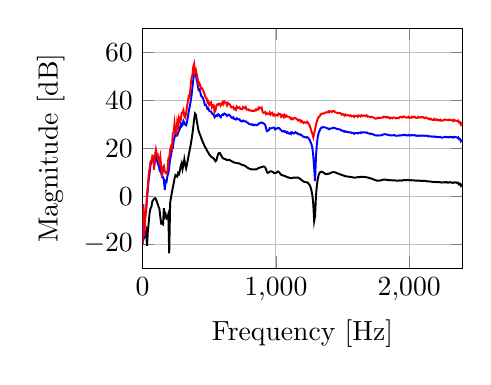
\begin{tikzpicture}

\begin{axis}[%
width=1.6in,
height=1.2in,
at={(1.011in,0.642in)},
scale only axis,
xmin=0,
xmax=2400,
xmajorgrids,
ymin=-30,
ymax=70,
ymajorgrids,
ylabel={Magnitude [dB]},
xlabel={Frequency [Hz]},
axis background/.style={fill=white}
]
\addplot [color=black,solid,line width=0.7pt,forget plot]
  table[row sep=crcr]{%
0	-20.0487587312399\\
6.66944096884746	-15.1198286488021\\
13.3388819376949	-17.0342399584206\\
20.0083229065424	-16.303194843339\\
26.6777638753898	-14.7962886511984\\
33.3472048442373	-20.6598371130847\\
40.0166458130848	-14.4557378448972\\
46.6860867819322	-10.7231796436896\\
53.3555277507797	-6.68929927164874\\
60.0249687196271	-5.00174395429775\\
66.6944096884746	-4.35120832215586\\
73.363850657322	-2.14327488039484\\
80.0332916261695	-1.6357351744986\\
86.702732595017	-1.08244168916939\\
93.3721735638644	-0.784791293115845\\
100.041614532712	-1.1515485217107\\
106.711055501559	-2.23392951885352\\
113.380496470407	-3.25334805655735\\
120.049937439254	-4.28723268538043\\
126.719378408102	-5.37856269568507\\
133.388819376949	-8.68574264179734\\
140.058260345797	-11.4500332968668\\
146.727701314644	-11.4038053561626\\
153.397142283492	-11.7245402057755\\
160.066583252339	-5.0055269896238\\
166.736024221186	-8.44545337311039\\
173.405465190034	-7.57504950140747\\
180.074906158881	-9.24310764770295\\
186.744347127729	-8.80698899348521\\
193.413788096576	-7.52181346110201\\
200.083229065424	-23.8498097372691\\
206.752670034271	-2.89005609350758\\
213.422111003119	-0.482574852395068\\
220.091551971966	1.60203735985558\\
226.760992940814	3.47424986688718\\
233.430433909661	5.29663217829555\\
240.099874878509	7.40902951539864\\
246.769315847356	8.79260541102708\\
253.438756816203	8.42229233177448\\
260.108197785051	8.1621822849779\\
266.777638753898	9.71860050383648\\
273.447079722746	9.24805783652312\\
280.116520691593	10.5461884815772\\
286.785961660441	12.7462393484334\\
293.455402629288	13.8128344559473\\
300.124843598136	11.3562980225335\\
306.794284566983	13.0225331345595\\
313.463725535831	15.3878277905346\\
320.133166504678	13.3487733331614\\
326.802607473525	11.618116409216\\
333.472048442373	13.2756561673794\\
340.14148941122	15.297365359007\\
346.810930380068	17.3666597314884\\
353.480371348915	19.1861707835379\\
360.149812317763	21.1548208550903\\
366.81925328661	23.2781736469893\\
373.488694255458	25.7795010023069\\
380.158135224305	28.7053918086881\\
386.827576193153	32.0846853382303\\
393.497017162	34.4267175381787\\
400.166458130848	33.9505458128728\\
406.835899099695	31.4873550826056\\
413.505340068542	29.2170117011374\\
420.17478103739	27.3019127159821\\
426.844222006237	26.1797366493716\\
433.513662975085	25.3157313050429\\
440.183103943932	24.2057182984711\\
446.85254491278	23.290395783258\\
453.521985881627	22.3878979183417\\
460.191426850475	21.60415932599\\
466.860867819322	20.7709829065924\\
473.53030878817	20.0885558968387\\
480.199749757017	19.4323228642096\\
486.869190725864	18.6908379824591\\
493.538631694712	18.1240856471387\\
500.208072663559	17.4169934799121\\
506.877513632407	16.986634280519\\
513.546954601254	16.4993581905569\\
520.216395570102	16.1919521224916\\
526.885836538949	16.0182134672153\\
533.555277507797	15.8037005327483\\
540.224718476644	15.1219659228159\\
546.894159445492	14.5825111378862\\
553.563600414339	14.9249330668376\\
560.233041383186	16.3345574651993\\
566.902482352034	17.5314472890824\\
573.571923320881	18.0466676213715\\
580.241364289729	17.9752767658784\\
586.910805258576	17.2620914846372\\
593.580246227424	16.6078538766868\\
600.249687196271	16.0282214291011\\
606.919128165119	15.6892443753367\\
613.588569133966	15.5882313206699\\
620.258010102814	15.4977489853147\\
626.927451071661	15.2498244875837\\
633.596892040508	15.0304027543537\\
640.266333009356	15.0950717833943\\
646.935773978203	15.2206054457582\\
653.605214947051	15.0570826579417\\
660.274655915898	14.8581503712255\\
666.944096884746	14.6159864112486\\
673.613537853593	14.4145622453499\\
680.282978822441	14.2407617757287\\
686.952419791288	14.0477359248121\\
693.621860760136	13.9845541892167\\
700.291301728983	13.9156960952036\\
706.960742697831	13.8209864026508\\
713.630183666678	13.7252040922125\\
720.299624635525	13.719919039345\\
726.969065604373	13.6610343852311\\
733.63850657322	13.4082141441493\\
740.307947542068	13.1756866771715\\
746.977388510915	13.0493516140333\\
753.646829479763	13.0081459317708\\
760.31627044861	12.8890321676709\\
766.985711417458	12.6553655249787\\
773.655152386305	12.5065721297099\\
780.324593355153	12.1476594869726\\
786.994034324	11.8745908760281\\
793.663475292847	11.7034903712762\\
800.332916261695	11.4985774792138\\
807.002357230542	11.3837332881055\\
813.67179819939	11.2277439431574\\
820.341239168237	11.2087216765361\\
827.010680137085	11.165959581749\\
833.680121105932	11.1324522724851\\
840.34956207478	11.2018621293156\\
847.019003043627	11.2058359789266\\
853.688444012475	11.220594143102\\
860.357884981322	11.385158335654\\
867.02732595017	11.6618138985397\\
873.696766919017	11.8074366257923\\
880.366207887864	11.9369555767766\\
887.035648856712	12.0897644436753\\
893.705089825559	12.1478349676403\\
900.374530794407	12.293869204835\\
907.043971763254	12.3962434453679\\
913.713412732102	12.2599054813914\\
920.382853700949	11.9560863463259\\
927.052294669797	11.0727027842254\\
933.721735638644	9.96470300024418\\
940.391176607492	9.75565988680186\\
947.060617576339	9.8817312233776\\
953.730058545186	10.2635241464301\\
960.399499514034	10.342564450562\\
967.068940482881	10.3395878261441\\
973.738381451729	10.1898658552898\\
980.407822420576	9.8934905161314\\
987.077263389424	9.66581752460281\\
993.746704358271	9.62786392512574\\
1000.41614532712	9.75615585236342\\
1007.08558629597	9.93971063557813\\
1013.75502726481	10.3422119903628\\
1020.42446823366	10.1980394823397\\
1027.09390920251	9.77924856044184\\
1033.76335017136	9.27605023907571\\
1040.4327911402	8.9026715525102\\
1047.10223210905	8.80362080534128\\
1053.7716730779	8.65318909923104\\
1060.44111404675	8.49430175012251\\
1067.11055501559	8.47806688429255\\
1073.77999598444	8.24819989854638\\
1080.44943695329	8.11312313460769\\
1087.11887792214	7.88692743852098\\
1093.78831889098	7.85693715538574\\
1100.45775985983	7.69465983381162\\
1107.12720082868	7.53269317692368\\
1113.79664179753	7.49971429912328\\
1120.46608276637	7.61271205995918\\
1127.13552373522	7.66843451521201\\
1133.80496470407	7.79602908681334\\
1140.47440567292	7.70448271239874\\
1147.14384664176	7.73221492909188\\
1153.81328761061	7.73181066779452\\
1160.48272857946	7.71857363461331\\
1167.15216954831	7.76954134955827\\
1173.82161051715	7.56221590613739\\
1180.491051486	7.23164524837447\\
1187.16049245485	7.0445338089638\\
1193.82993342369	6.68149349857916\\
1200.49937439254	6.4449899730087\\
1207.16881536139	6.10312875796965\\
1213.83825633024	6.0097646953722\\
1220.50769729908	5.87025384588163\\
1227.17713826793	5.8058226272411\\
1233.84657923678	5.78040134867712\\
1240.51602020563	5.59884417499817\\
1247.18546117447	5.02065144141591\\
1253.85490214332	4.61997118096475\\
1260.52434311217	3.67633292433192\\
1267.19378408102	2.34330760449349\\
1273.86322504986	0.330148903396033\\
1280.53266601871	-3.33406711562751\\
1287.20210698756	-10.2975077225615\\
1293.87154795641	-8.23932116173958\\
1300.54098892525	-0.0504526894621943\\
1307.2104298941	4.41312707327818\\
1313.87987086295	7.16388601945597\\
1320.5493118318	8.8180810705879\\
1327.21875280064	9.64769916783657\\
1333.88819376949	10.1213708572002\\
1340.55763473834	10.2126537699231\\
1347.22707570719	10.086236888369\\
1353.89651667603	9.96475533895285\\
1360.56595764488	9.68881796246233\\
1367.23539861373	9.45814374578669\\
1373.90483958258	9.21991209305461\\
1380.57428055142	9.22560189789232\\
1387.24372152027	9.25507050908739\\
1393.91316248912	9.39961014108227\\
1400.58260345797	9.40403399507104\\
1407.25204442681	9.5959632665098\\
1413.92148539566	9.81260026763373\\
1420.59092636451	9.9515380863488\\
1427.26036733336	10.0084243176538\\
1433.9298083022	10.076913415341\\
1440.59924927105	9.96583673695072\\
1447.2686902399	9.85390572621115\\
1453.93813120875	9.77057303062154\\
1460.60757217759	9.56658183325933\\
1467.27701314644	9.40119349335695\\
1473.94645411529	9.32365204414415\\
1480.61589508414	9.1400356094238\\
1487.28533605298	8.9782642045505\\
1493.95477702183	8.88490656734342\\
1500.62421799068	8.75658483707809\\
1507.29365895953	8.64394834471857\\
1513.96309992837	8.47813597782596\\
1520.63254089722	8.36366672323785\\
1527.30198186607	8.25947876297518\\
1533.97142283492	8.24130376763184\\
1540.64086380376	8.18123526644235\\
1547.31030477261	8.1022955122158\\
1553.97974574146	8.04006587529611\\
1560.64918671031	8.03334733158801\\
1567.31862767915	7.98098505634755\\
1573.988068648	7.88111469269561\\
1580.65750961685	7.8513820734062\\
1587.32695058569	7.73030446704829\\
1593.99639155454	7.74954898960166\\
1600.66583252339	7.81454036991847\\
1607.33527349224	7.83281535246582\\
1614.00471446108	7.94265737575515\\
1620.67415542993	7.98138741022576\\
1627.34359639878	7.98508389625216\\
1634.01303736763	8.04999617504294\\
1640.68247833647	8.10021289468602\\
1647.35191930532	8.06892639991748\\
1654.02136027417	8.05546864143061\\
1660.69080124302	8.06279491665488\\
1667.36024221186	7.97686673480105\\
1674.02968318071	7.95207358408032\\
1680.69912414956	7.90246757767181\\
1687.36856511841	7.77732599874859\\
1694.03800608725	7.74235995684231\\
1700.7074470561	7.57148021158726\\
1707.37688802495	7.51907183905363\\
1714.0463289938	7.34302575137448\\
1720.71576996264	7.29622254883677\\
1727.38521093149	7.10708183439396\\
1734.05465190034	6.99184506410273\\
1740.72409286919	6.81585864666285\\
1747.39353383803	6.73925074141611\\
1754.06297480688	6.51634814954277\\
1760.73241577573	6.5046366441454\\
1767.40185674458	6.51534274521224\\
1774.07129771342	6.49778597055656\\
1780.74073868227	6.5027309147596\\
1787.41017965112	6.66096272956585\\
1794.07962061997	6.68599174262566\\
1800.74906158881	6.7859138904786\\
1807.41850255766	6.93749707775066\\
1814.08794352651	6.93925297520513\\
1820.75738449536	6.92244091960105\\
1827.4268254642	6.88417990649145\\
1834.09626643305	6.72060751795472\\
1840.7657074019	6.68313612027974\\
1847.43514837075	6.76439558492782\\
1854.10458933959	6.62118179284594\\
1860.77403030844	6.67666591156341\\
1867.44347127729	6.66742931604751\\
1874.11291224614	6.61812127334921\\
1880.78235321498	6.57379594203512\\
1887.45179418383	6.6252911037417\\
1894.12123515268	6.58083432296879\\
1900.79067612153	6.52814176468354\\
1907.46011709037	6.50124438101973\\
1914.12955805922	6.53921917902875\\
1920.79899902807	6.50564465486567\\
1927.46843999692	6.59670977440938\\
1934.13788096576	6.5808210246406\\
1940.80732193461	6.5207010147943\\
1947.47676290346	6.51506968513275\\
1954.14620387231	6.73310819944533\\
1960.81564484115	6.71013860894114\\
1967.48508581	6.64903913507737\\
1974.15452677885	6.74812319759256\\
1980.82396774769	6.71068768316015\\
1987.49340871654	6.66610261621373\\
1994.16284968539	6.76891694050447\\
2000.83229065424	6.6491896391241\\
2007.50173162308	6.61585957804051\\
2014.17117259193	6.69663297716651\\
2020.84061356078	6.63556782623735\\
2027.51005452963	6.61496288121215\\
2034.17949549847	6.65314733859702\\
2040.84893646732	6.56253815480099\\
2047.51837743617	6.52719414236225\\
2054.18781840502	6.53288683163146\\
2060.85725937386	6.44397445046302\\
2067.52670034271	6.52132437447671\\
2074.19614131156	6.45651887990799\\
2080.86558228041	6.49180231444652\\
2087.53502324925	6.37556254246593\\
2094.2044642181	6.38835955815856\\
2100.87390518695	6.38800999197321\\
2107.5433461558	6.41869017506372\\
2114.21278712464	6.45696129007083\\
2120.88222809349	6.38399284967227\\
2127.55166906234	6.30427827094713\\
2134.22111003119	6.19580379642489\\
2140.89055100003	6.23445392444571\\
2147.55999196888	6.138755636176\\
2154.22943293773	6.15874396802726\\
2160.89887390658	6.08763548342839\\
2167.56831487542	6.03555632613822\\
2174.23775584427	5.98609086606414\\
2180.90719681312	6.02482885091038\\
2187.57663778197	5.91142930127247\\
2194.24607875081	5.90620837397779\\
2200.91551971966	5.97642482649767\\
2207.58496068851	5.8267910718678\\
2214.25440165736	5.89031841840725\\
2220.9238426262	5.89135869621277\\
2227.59328359505	5.89733460682358\\
2234.2627245639	5.80541657746534\\
2240.93216553275	5.68604121080201\\
2247.60160650159	5.75738242073362\\
2254.27104747044	5.79181508953615\\
2260.94048843929	5.72435541249592\\
2267.60992940814	5.91887483795505\\
2274.27937037698	5.74323479651245\\
2280.94881134583	5.915516734774\\
2287.61825231468	5.678546930139\\
2294.28769328353	5.66300396208394\\
2300.95713425237	5.8598982127844\\
2307.62657522122	5.83660940155178\\
2314.29601619007	5.65455921049519\\
2320.96545715892	5.72882209801376\\
2327.63489812776	5.55231206649722\\
2334.30433909661	5.77650458704093\\
2340.97378006546	5.67908113685681\\
2347.64322103431	5.80773692997328\\
2354.31266200315	5.69838419206977\\
2360.982102972	5.40321555955911\\
2367.65154394085	5.64298798739372\\
2374.3209849097	4.92864224564267\\
2380.99042587854	5.18402670886947\\
2387.65986684739	4.4041843097699\\
2394.32930781624	5.21405865383168\\
};
\addplot [color=blue,line width=0.7pt,solid,forget plot]
  table[row sep=crcr]{%
0	-19.1801970800519\\
6.66944096884746	-12.8703566346097\\
13.3388819376949	-14.9767747928368\\
20.0083229065424	-8.1169528748585\\
26.6777638753898	-6.02007700819861\\
33.3472048442373	-0.983876052705199\\
40.0166458130848	3.03834920475862\\
46.6860867819322	7.17636581805885\\
53.3555277507797	9.86526177201357\\
60.0249687196271	13.1463387708932\\
66.6944096884746	13.8757372547918\\
73.363850657322	15.3344350669251\\
80.0332916261695	15.5103872374769\\
86.702732595017	16.425478329494\\
93.3721735638644	14.7417155654727\\
100.041614532712	16.8909416893169\\
106.711055501559	15.1693140361402\\
113.380496470407	13.8378835887887\\
120.049937439254	12.8763175666628\\
126.719378408102	11.2245842269512\\
133.388819376949	12.2755448015368\\
140.058260345797	9.76444174431159\\
146.727701314644	7.9812499771494\\
153.397142283492	7.89449997979367\\
160.066583252339	6.76913976316376\\
166.736024221186	2.64501448882146\\
173.405465190034	6.32166739159555\\
180.074906158881	6.03588448839818\\
186.744347127729	8.53733258644788\\
193.413788096576	9.60386927649499\\
200.083229065424	11.9079525145153\\
206.752670034271	15.5768450064805\\
213.422111003119	16.8564773229072\\
220.091551971966	19.4056208174385\\
226.760992940814	20.0977881758406\\
233.430433909661	23.0867696537098\\
240.099874878509	24.5133525415327\\
246.769315847356	26.0318705836573\\
253.438756816203	25.2159191534437\\
260.108197785051	25.3004400529391\\
266.777638753898	26.3567739565968\\
273.447079722746	27.4030394355481\\
280.116520691593	28.0266175894058\\
286.785961660441	30.3237158950793\\
293.455402629288	29.2015400170774\\
300.124843598136	29.6615334869133\\
306.794284566983	31.3788778937628\\
313.463725535831	30.6152438924125\\
320.133166504678	29.7759228465178\\
326.802607473525	29.5619250778803\\
333.472048442373	31.0231998781484\\
340.14148941122	32.9915165065272\\
346.810930380068	35.5603667608652\\
353.480371348915	37.1554836973345\\
360.149812317763	39.2773434425713\\
366.81925328661	41.5981250326168\\
373.488694255458	44.9696288263719\\
380.158135224305	48.3111948726315\\
386.827576193153	51.2585070598154\\
393.497017162	51.2682639867973\\
400.166458130848	50.243525737973\\
406.835899099695	48.4862480361356\\
413.505340068542	46.2836446546836\\
420.17478103739	44.3104281370761\\
426.844222006237	44.5172237794285\\
433.513662975085	43.2209471111121\\
440.183103943932	41.6709460714875\\
446.85254491278	41.4697262151817\\
453.521985881627	40.7647867182055\\
460.191426850475	39.6633007472136\\
466.860867819322	38.0957284486303\\
473.53030878817	38.169121432027\\
480.199749757017	37.4519012732778\\
486.869190725864	36.3727934222095\\
493.538631694712	36.5546229678987\\
500.208072663559	35.5969432067736\\
506.877513632407	35.367941821441\\
513.546954601254	35.2417809028389\\
520.216395570102	34.6477493524093\\
526.885836538949	34.1244046315677\\
533.555277507797	34.1031174062651\\
540.224718476644	32.9038375330107\\
546.894159445492	33.3928388176014\\
553.563600414339	33.7323160866798\\
560.233041383186	33.4368130917103\\
566.902482352034	34.1904953640828\\
573.571923320881	33.931489848504\\
580.241364289729	33.3392737176728\\
586.910805258576	32.8984144124481\\
593.580246227424	33.7433695622489\\
600.249687196271	34.1178753654268\\
606.919128165119	33.9336683252705\\
613.588569133966	34.4485544577773\\
620.258010102814	34.2843657671703\\
626.927451071661	34.060214309503\\
633.596892040508	33.4349764550008\\
640.266333009356	33.8646627251901\\
646.935773978203	33.9786137674422\\
653.605214947051	33.7465785637577\\
660.274655915898	33.3109087036117\\
666.944096884746	32.7438776079588\\
673.613537853593	32.568638059062\\
680.282978822441	32.9108736275211\\
686.952419791288	32.2249942772816\\
693.621860760136	32.1142750583997\\
700.291301728983	31.9571324211216\\
706.960742697831	32.4892728441236\\
713.630183666678	32.1435994092285\\
720.299624635525	32.021746854411\\
726.969065604373	32.0710323808955\\
733.63850657322	31.4267831219643\\
740.307947542068	31.1772695382483\\
746.977388510915	31.162518285872\\
753.646829479763	31.5393637388437\\
760.31627044861	31.2973953950049\\
766.985711417458	31.2182846338879\\
773.655152386305	31.2160961127834\\
780.324593355153	30.8348945075471\\
786.994034324	30.7286324748179\\
793.663475292847	30.382857168758\\
800.332916261695	30.0744778419275\\
807.002357230542	29.9962664433648\\
813.67179819939	29.962698019713\\
820.341239168237	29.6686337884023\\
827.010680137085	29.9415857655778\\
833.680121105932	29.665781211827\\
840.34956207478	29.6266816144405\\
847.019003043627	29.8283984647226\\
853.688444012475	29.6297069262368\\
860.357884981322	29.6061515105809\\
867.02732595017	29.9255274703579\\
873.696766919017	30.3836449587776\\
880.366207887864	30.4195349481781\\
887.035648856712	30.6293093173666\\
893.705089825559	30.7583945440376\\
900.374530794407	30.4889757351797\\
907.043971763254	30.3845402431785\\
913.713412732102	30.04889124241\\
920.382853700949	29.6944489814507\\
927.052294669797	28.0784153048193\\
933.721735638644	27.1086812359051\\
940.391176607492	27.3559333536648\\
947.060617576339	27.5405458598276\\
953.730058545186	28.3388139097659\\
960.399499514034	28.2741413233711\\
967.068940482881	28.316457653925\\
973.738381451729	28.5072210913902\\
980.407822420576	28.5600053986234\\
987.077263389424	28.5737552132371\\
993.746704358271	27.8398963271317\\
1000.41614532712	28.0898809053163\\
1007.08558629597	28.1965674308498\\
1013.75502726481	28.4628748764566\\
1020.42446823366	28.4109689957096\\
1027.09390920251	28.3068645746434\\
1033.76335017136	27.7346741698898\\
1040.4327911402	27.4788041500008\\
1047.10223210905	27.0100829685413\\
1053.7716730779	26.9924831726905\\
1060.44111404675	27.2004924387251\\
1067.11055501559	26.849233187843\\
1073.77999598444	26.9830257865469\\
1080.44943695329	26.4670906903599\\
1087.11887792214	26.7454074919348\\
1093.78831889098	26.1231981345171\\
1100.45775985983	26.0690493476289\\
1107.12720082868	26.4257190724241\\
1113.79664179753	25.9698837825955\\
1120.46608276637	26.6504318008235\\
1127.13552373522	26.3755217205762\\
1133.80496470407	26.1354915787008\\
1140.47440567292	26.4380891246027\\
1147.14384664176	26.6813208161658\\
1153.81328761061	26.2404976832252\\
1160.48272857946	26.322558600175\\
1167.15216954831	25.8835037848182\\
1173.82161051715	25.7364256243679\\
1180.491051486	25.8250596096695\\
1187.16049245485	25.4196005650628\\
1193.82993342369	25.4691538328777\\
1200.49937439254	25.0421318570829\\
1207.16881536139	24.7441917848824\\
1213.83825633024	24.5748943582446\\
1220.50769729908	24.5925564266071\\
1227.17713826793	24.4302692146368\\
1233.84657923678	24.6810745589517\\
1240.51602020563	24.397307782136\\
1247.18546117447	23.908083233262\\
1253.85490214332	23.4238712415594\\
1260.52434311217	22.5052907976336\\
1267.19378408102	21.5606708818796\\
1273.86322504986	20.0584900520215\\
1280.53266601871	16.6940016155194\\
1287.20210698756	11.6522752349905\\
1293.87154795641	6.30451494354049\\
1300.54098892525	16.4372208246285\\
1307.2104298941	21.5531699253565\\
1313.87987086295	24.6671956263859\\
1320.5493118318	26.3379178804065\\
1327.21875280064	27.1813964983545\\
1333.88819376949	28.0484733159775\\
1340.55763473834	28.6069160984365\\
1347.22707570719	28.5982246304511\\
1353.89651667603	28.8769385917799\\
1360.56595764488	28.7223173527069\\
1367.23539861373	28.6659731656965\\
1373.90483958258	28.5922594637542\\
1380.57428055142	28.4587951765109\\
1387.24372152027	28.2085080700907\\
1393.91316248912	28.2150230654651\\
1400.58260345797	27.8900350269182\\
1407.25204442681	28.1925719408122\\
1413.92148539566	28.2419799953219\\
1420.59092636451	28.2829268523402\\
1427.26036733336	28.4634872164612\\
1433.9298083022	28.5907769115149\\
1440.59924927105	28.3814763609529\\
1447.2686902399	28.3226799307106\\
1453.93813120875	28.1356741426561\\
1460.60757217759	27.9685526227807\\
1467.27701314644	27.9678715914959\\
1473.94645411529	27.8909541343816\\
1480.61589508414	27.8238766711262\\
1487.28533605298	27.6014302681019\\
1493.95477702183	27.2717380592555\\
1500.62421799068	27.3018413746368\\
1507.29365895953	27.1995224671422\\
1513.96309992837	26.8397200608697\\
1520.63254089722	27.0829515584527\\
1527.30198186607	26.8503571067805\\
1533.97142283492	26.756386803348\\
1540.64086380376	26.7898604834281\\
1547.31030477261	26.6321969857586\\
1553.97974574146	26.6120446351326\\
1560.64918671031	26.6522550973329\\
1567.31862767915	26.3323931160699\\
1573.988068648	26.4295250363119\\
1580.65750961685	26.343839184407\\
1587.32695058569	26.0015876489182\\
1593.99639155454	26.3300221476214\\
1600.66583252339	26.3039705741923\\
1607.33527349224	26.3742650558845\\
1614.00471446108	26.1463871584589\\
1620.67415542993	26.4418942251999\\
1627.34359639878	26.4672180007292\\
1634.01303736763	26.2792446290963\\
1640.68247833647	26.6436284243602\\
1647.35191930532	26.5095040190372\\
1654.02136027417	26.6573687967465\\
1660.69080124302	26.5620677867498\\
1667.36024221186	26.5989978419798\\
1674.02968318071	26.4764653674816\\
1680.69912414956	26.6013987294364\\
1687.36856511841	26.2507565066588\\
1694.03800608725	26.250822684696\\
1700.7074470561	26.1437788317374\\
1707.37688802495	26.0138276096747\\
1714.0463289938	26.0000044652493\\
1720.71576996264	25.9766429547442\\
1727.38521093149	25.7852372119412\\
1734.05465190034	25.6845896433477\\
1740.72409286919	25.4260848492213\\
1747.39353383803	25.3815678004591\\
1754.06297480688	25.3994084234738\\
1760.73241577573	25.2465614318773\\
1767.40185674458	25.3585533383756\\
1774.07129771342	25.2934182835509\\
1780.74073868227	25.3332686921627\\
1787.41017965112	25.3315671007097\\
1794.07962061997	25.4529797134563\\
1800.74906158881	25.5886581256154\\
1807.41850255766	25.8112219394707\\
1814.08794352651	25.8336747007692\\
1820.75738449536	25.8512388544852\\
1827.4268254642	25.6812476695809\\
1834.09626643305	25.7200303426687\\
1840.7657074019	25.5997689689591\\
1847.43514837075	25.6166191632788\\
1854.10458933959	25.361021151081\\
1860.77403030844	25.4169823389784\\
1867.44347127729	25.3575452873573\\
1874.11291224614	25.3531107579859\\
1880.78235321498	25.4061044547324\\
1887.45179418383	25.4934789583337\\
1894.12123515268	25.2934729566871\\
1900.79067612153	25.150524012892\\
1907.46011709037	25.2282774494811\\
1914.12955805922	25.2017626260044\\
1920.79899902807	25.2044661735462\\
1927.46843999692	25.3815455806729\\
1934.13788096576	25.3764459878828\\
1940.80732193461	25.385750006199\\
1947.47676290346	25.3633905907365\\
1954.14620387231	25.5519570739233\\
1960.81564484115	25.6353093777738\\
1967.48508581	25.4451022627762\\
1974.15452677885	25.4541836251086\\
1980.82396774769	25.337687037348\\
1987.49340871654	25.3510653476931\\
1994.16284968539	25.5605415694349\\
2000.83229065424	25.2743306829669\\
2007.50173162308	25.3800826099287\\
2014.17117259193	25.3329161570438\\
2020.84061356078	25.5531143426426\\
2027.51005452963	25.3941264714679\\
2034.17949549847	25.347106390821\\
2040.84893646732	25.4895692062649\\
2047.51837743617	25.2661215623274\\
2054.18781840502	25.2210476794\\
2060.85725937386	25.1367687606202\\
2067.52670034271	25.3569013486922\\
2074.19614131156	25.1900684754222\\
2080.86558228041	25.1789893140517\\
2087.53502324925	25.2859951981971\\
2094.2044642181	25.172839426885\\
2100.87390518695	25.2515733216014\\
2107.5433461558	25.2880714341211\\
2114.21278712464	25.1545719013543\\
2120.88222809349	25.2268960929446\\
2127.55166906234	25.2355614416271\\
2134.22111003119	25.0702603234227\\
2140.89055100003	25.1476689770138\\
2147.55999196888	24.9247159902261\\
2154.22943293773	24.922689731992\\
2160.89887390658	24.9955133770923\\
2167.56831487542	24.8149518125789\\
2174.23775584427	24.8259792113246\\
2180.90719681312	24.7869406198621\\
2187.57663778197	24.9333284802604\\
2194.24607875081	24.7182320239595\\
2200.91551971966	24.7419174388744\\
2207.58496068851	24.7876142318302\\
2214.25440165736	24.6259659842357\\
2220.9238426262	24.6350924557445\\
2227.59328359505	24.598620967243\\
2234.2627245639	24.7247842187087\\
2240.93216553275	24.4098973625254\\
2247.60160650159	24.4556792725291\\
2254.27104747044	24.5283713595465\\
2260.94048843929	24.5861744693618\\
2267.60992940814	24.7581537657624\\
2274.27937037698	24.6396803738645\\
2280.94881134583	24.654846607342\\
2287.61825231468	24.5997381831205\\
2294.28769328353	24.5289027956748\\
2300.95713425237	24.7571708595127\\
2307.62657522122	24.5896255439116\\
2314.29601619007	24.6110451864451\\
2320.96545715892	24.667921486107\\
2327.63489812776	24.3877408742219\\
2334.30433909661	24.7693625782859\\
2340.97378006546	24.6509753376336\\
2347.64322103431	24.6243542594069\\
2354.31266200315	24.545777701483\\
2360.982102972	24.3907721668534\\
2367.65154394085	24.5803582147782\\
2374.3209849097	23.7571480890376\\
2380.99042587854	23.8421940134045\\
2387.65986684739	22.9126274129111\\
2394.32930781624	23.5765876365837\\
};
\addplot [color=red,line width=0.7pt,solid,forget plot]
  table[row sep=crcr]{%
0	-19.7731498838748\\
6.66944096884746	-3.30129229121397\\
13.3388819376949	-16.5196915187148\\
20.0083229065424	-9.14668053363022\\
26.6777638753898	-5.76166775232025\\
33.3472048442373	0.715997976350927\\
40.0166458130848	4.67569859122506\\
46.6860867819322	9.3061016685291\\
53.3555277507797	11.6803761046995\\
60.0249687196271	14.5668135581482\\
66.6944096884746	14.7654268062205\\
73.363850657322	16.719238826743\\
80.0332916261695	16.1424633419342\\
86.702732595017	11.0575281883368\\
93.3721735638644	17.1794418502135\\
100.041614532712	19.4302729226033\\
106.711055501559	17.1647243810114\\
113.380496470407	17.4336984563287\\
120.049937439254	14.8178077949204\\
126.719378408102	14.0940850084646\\
133.388819376949	16.3749922926234\\
140.058260345797	12.5351765733749\\
146.727701314644	8.12594321424465\\
153.397142283492	11.8920519865686\\
160.066583252339	12.5716166006834\\
166.736024221186	10.285037659743\\
173.405465190034	9.70252691083641\\
180.074906158881	9.57652623134213\\
186.744347127729	10.638286473325\\
193.413788096576	15.8057440036925\\
200.083229065424	16.2967711522382\\
206.752670034271	19.4251561642881\\
213.422111003119	20.6816823950601\\
220.091551971966	19.8519442653404\\
226.760992940814	26.1082556453237\\
233.430433909661	26.6500868664063\\
240.099874878509	30.404475221027\\
246.769315847356	26.825393131967\\
253.438756816203	26.1285404111887\\
260.108197785051	30.9570292670671\\
266.777638753898	29.2117125593558\\
273.447079722746	32.6064626863794\\
280.116520691593	31.2360770691429\\
286.785961660441	31.722505229895\\
293.455402629288	34.6999692669045\\
300.124843598136	34.9927928087575\\
306.794284566983	35.8925128734339\\
313.463725535831	33.3145155986805\\
320.133166504678	32.8004219522627\\
326.802607473525	34.6908681946822\\
333.472048442373	37.2792444982084\\
340.14148941122	39.6336780746653\\
346.810930380068	41.6658226560305\\
353.480371348915	41.2799335430523\\
360.149812317763	45.6293609227908\\
366.81925328661	49.1313794764531\\
373.488694255458	50.4146591961717\\
380.158135224305	53.8841719664011\\
386.827576193153	55.1607782592531\\
393.497017162	51.6507310675641\\
400.166458130848	52.5696601172965\\
406.835899099695	50.685373547418\\
413.505340068542	48.8997703515724\\
420.17478103739	46.055352278522\\
426.844222006237	46.9843441763525\\
433.513662975085	46.0167755931766\\
440.183103943932	44.7586647963142\\
446.85254491278	44.899210692511\\
453.521985881627	44.2825029563711\\
460.191426850475	43.3405779426588\\
466.860867819322	42.2331601158757\\
473.53030878817	40.9054822858416\\
480.199749757017	40.8005939018429\\
486.869190725864	39.1794932936421\\
493.538631694712	39.5687046720476\\
500.208072663559	38.0284570137054\\
506.877513632407	38.6610399513643\\
513.546954601254	39.0673385461637\\
520.216395570102	37.1510698815421\\
526.885836538949	37.9929142604868\\
533.555277507797	37.8986469335816\\
540.224718476644	35.0617599237344\\
546.894159445492	35.684870669366\\
553.563600414339	37.7578937591971\\
560.233041383186	38.24050111937\\
566.902482352034	38.016164070372\\
573.571923320881	38.6115137612817\\
580.241364289729	38.5083844553459\\
586.910805258576	37.7271324115351\\
593.580246227424	38.4959940201515\\
600.249687196271	39.142060156938\\
606.919128165119	38.3708394010276\\
613.588569133966	39.4929000003076\\
620.258010102814	39.0343745804699\\
626.927451071661	39.0045192335195\\
633.596892040508	37.87804477622\\
640.266333009356	38.8658497847705\\
646.935773978203	38.5200866414581\\
653.605214947051	38.2617127986245\\
660.274655915898	37.6673340406495\\
666.944096884746	36.942659357658\\
673.613537853593	37.0599783142805\\
680.282978822441	37.2310736462357\\
686.952419791288	36.2838048671267\\
693.621860760136	36.550554058913\\
700.291301728983	35.9917952535513\\
706.960742697831	37.3200057510477\\
713.630183666678	36.793136905267\\
720.299624635525	36.8249417546396\\
726.969065604373	37.0781762663894\\
733.63850657322	36.4125402477533\\
740.307947542068	36.3121785296935\\
746.977388510915	36.2451162273039\\
753.646829479763	37.2084380506257\\
760.31627044861	36.9206850342757\\
766.985711417458	36.6914275508524\\
773.655152386305	37.2095095164535\\
780.324593355153	36.104968563149\\
786.994034324	36.048838049227\\
793.663475292847	36.190495756928\\
800.332916261695	35.7104287884522\\
807.002357230542	35.8242109649086\\
813.67179819939	35.6991761345302\\
820.341239168237	35.4503876709311\\
827.010680137085	35.6718081181175\\
833.680121105932	35.5252868419793\\
840.34956207478	35.5637592153987\\
847.019003043627	36.1216316480192\\
853.688444012475	35.8541719470195\\
860.357884981322	36.3190619987209\\
867.02732595017	36.1211510307247\\
873.696766919017	37.056863223976\\
880.366207887864	36.651127915307\\
887.035648856712	36.5825166509355\\
893.705089825559	36.9504055566917\\
900.374530794407	35.1961814758886\\
907.043971763254	34.7039472643645\\
913.713412732102	34.8894998271584\\
920.382853700949	35.1129229272755\\
927.052294669797	34.2035062965127\\
933.721735638644	34.544536166122\\
940.391176607492	34.3161625921429\\
947.060617576339	34.2152352021431\\
953.730058545186	34.9725599786183\\
960.399499514034	34.0157821012478\\
967.068940482881	34.5575512902624\\
973.738381451729	34.7924069441786\\
980.407822420576	33.7202383105071\\
987.077263389424	34.0640499711664\\
993.746704358271	33.5499848673986\\
1000.41614532712	33.7602055880614\\
1007.08558629597	33.8794047458212\\
1013.75502726481	33.6000643803354\\
1020.42446823366	34.41709105744\\
1027.09390920251	34.1784844968047\\
1033.76335017136	34.213559194249\\
1040.4327911402	33.0793653419113\\
1047.10223210905	33.5387825724225\\
1053.7716730779	33.824912673582\\
1060.44111404675	32.9699657541057\\
1067.11055501559	33.8378469138417\\
1073.77999598444	33.2124005244341\\
1080.44943695329	33.5671937553562\\
1087.11887792214	33.1124632723943\\
1093.78831889098	33.1180967971584\\
1100.45775985983	33.1098632608928\\
1107.12720082868	32.6414362236894\\
1113.79664179753	32.1194058224594\\
1120.46608276637	32.5272282197209\\
1127.13552373522	32.0840721791977\\
1133.80496470407	32.4943251641124\\
1140.47440567292	32.5364569322681\\
1147.14384664176	32.5852481246147\\
1153.81328761061	32.1751862503957\\
1160.48272857946	31.9964871334953\\
1167.15216954831	31.5145565174944\\
1173.82161051715	31.9319084355698\\
1180.491051486	31.6954106176743\\
1187.16049245485	31.0173995293861\\
1193.82993342369	31.4179436596554\\
1200.49937439254	30.88197629505\\
1207.16881536139	30.4987820836591\\
1213.83825633024	30.8907166745812\\
1220.50769729908	30.669066786967\\
1227.17713826793	30.6088276123375\\
1233.84657923678	31.0230605872693\\
1240.51602020563	30.646974834486\\
1247.18546117447	30.0056944791357\\
1253.85490214332	29.3534461723242\\
1260.52434311217	28.2651209471615\\
1267.19378408102	26.954021048548\\
1273.86322504986	25.9012974545492\\
1280.53266601871	24.5716215147262\\
1287.20210698756	26.1838866071504\\
1293.87154795641	27.9640423038921\\
1300.54098892525	29.6587510669448\\
1307.2104298941	31.1844476112175\\
1313.87987086295	32.2512424614966\\
1320.5493118318	33.0744916232722\\
1327.21875280064	33.1938211374655\\
1333.88819376949	33.8594312519506\\
1340.55763473834	34.3239227849652\\
1347.22707570719	34.2903123904882\\
1353.89651667603	34.5362555107921\\
1360.56595764488	34.4735651034455\\
1367.23539861373	34.6424254058558\\
1373.90483958258	34.9998993126672\\
1380.57428055142	34.9445366157403\\
1387.24372152027	34.9212782294764\\
1393.91316248912	35.3210359275985\\
1400.58260345797	34.957042662985\\
1407.25204442681	35.4463006533749\\
1413.92148539566	35.3815415899574\\
1420.59092636451	35.1247290520045\\
1427.26036733336	35.483454745991\\
1433.9298083022	35.5680035110321\\
1440.59924927105	35.2443526361233\\
1447.2686902399	34.9585356085181\\
1453.93813120875	34.8467609647867\\
1460.60757217759	34.6729699561945\\
1467.27701314644	34.5901111077368\\
1473.94645411529	34.7679439086908\\
1480.61589508414	34.6966283625407\\
1487.28533605298	34.4917011620637\\
1493.95477702183	33.9895974859901\\
1500.62421799068	34.219971740426\\
1507.29365895953	34.0773365592971\\
1513.96309992837	33.5919233073209\\
1520.63254089722	34.05674398874\\
1527.30198186607	33.6836839894487\\
1533.97142283492	33.737728138333\\
1540.64086380376	33.8784614848418\\
1547.31030477261	33.6511509515165\\
1553.97974574146	33.4226620143495\\
1560.64918671031	33.6968369088947\\
1567.31862767915	33.276016797193\\
1573.988068648	33.5366942634168\\
1580.65750961685	33.5209888551424\\
1587.32695058569	33.0236853121862\\
1593.99639155454	33.5420262045134\\
1600.66583252339	33.492102025589\\
1607.33527349224	33.5873714387896\\
1614.00471446108	33.0923914795437\\
1620.67415542993	33.6676565539402\\
1627.34359639878	33.564976523811\\
1634.01303736763	33.260843386433\\
1640.68247833647	33.6986835385745\\
1647.35191930532	33.4190163219924\\
1654.02136027417	33.6411712118615\\
1660.69080124302	33.5615313638007\\
1667.36024221186	33.564357460058\\
1674.02968318071	33.3931136236589\\
1680.69912414956	33.7027218290536\\
1687.36856511841	33.153902660869\\
1694.03800608725	33.2556036519438\\
1700.7074470561	33.1633921770775\\
1707.37688802495	32.971772759543\\
1714.0463289938	33.0718132268812\\
1720.71576996264	33.0923277218807\\
1727.38521093149	32.8549585330854\\
1734.05465190034	32.7263913958038\\
1740.72409286919	32.4113821233463\\
1747.39353383803	32.3581318999144\\
1754.06297480688	32.5013000771757\\
1760.73241577573	32.397506990593\\
1767.40185674458	32.762027196197\\
1774.07129771342	32.6426044719977\\
1780.74073868227	32.5927768254359\\
1787.41017965112	32.6550171941744\\
1794.07962061997	32.7793490227485\\
1800.74906158881	32.7079221015991\\
1807.41850255766	33.1481905312322\\
1814.08794352651	33.0278793087225\\
1820.75738449536	33.1230239360321\\
1827.4268254642	32.8213517278662\\
1834.09626643305	33.0357032185694\\
1840.7657074019	32.7839350712744\\
1847.43514837075	32.9292949378254\\
1854.10458933959	32.4314197720893\\
1860.77403030844	32.7096293453212\\
1867.44347127729	32.6528396080951\\
1874.11291224614	32.446351701142\\
1880.78235321498	32.7719434715459\\
1887.45179418383	32.8660899906374\\
1894.12123515268	32.7054232709123\\
1900.79067612153	32.4172726216336\\
1907.46011709037	32.5655138262646\\
1914.12955805922	32.6899357772568\\
1920.79899902807	32.4907240301219\\
1927.46843999692	32.9278271785415\\
1934.13788096576	33.0360239620291\\
1940.80732193461	33.0176444262547\\
1947.47676290346	32.7593496869112\\
1954.14620387231	33.1663282462649\\
1960.81564484115	33.2507591912716\\
1967.48508581	32.972874509728\\
1974.15452677885	32.8277872601022\\
1980.82396774769	32.7746222144784\\
1987.49340871654	32.734742518744\\
1994.16284968539	33.1215205897337\\
2000.83229065424	32.6914518434221\\
2007.50173162308	32.7559968712182\\
2014.17117259193	32.677494916305\\
2020.84061356078	33.1664443003249\\
2027.51005452963	32.8962902999062\\
2034.17949549847	32.8384791907013\\
2040.84893646732	33.1302460915559\\
2047.51837743617	32.7275270964612\\
2054.18781840502	32.7021585046661\\
2060.85725937386	32.6287144507275\\
2067.52670034271	33.0835777879169\\
2074.19614131156	32.794345139603\\
2080.86558228041	32.7793950077453\\
2087.53502324925	32.9691533338572\\
2094.2044642181	32.8349283445452\\
2100.87390518695	33.0040625609765\\
2107.5433461558	32.9034999051104\\
2114.21278712464	32.5325190511779\\
2120.88222809349	32.7901048188627\\
2127.55166906234	32.7906003194698\\
2134.22111003119	32.4246517958174\\
2140.89055100003	32.4716819019555\\
2147.55999196888	32.0984015814186\\
2154.22943293773	32.0613549788269\\
2160.89887390658	32.3383445893988\\
2167.56831487542	31.8703975029692\\
2174.23775584427	31.8429764048798\\
2180.90719681312	31.8019842458616\\
2187.57663778197	32.2476589009584\\
2194.24607875081	31.8144992473476\\
2200.91551971966	31.8431698502412\\
2207.58496068851	32.0456705923427\\
2214.25440165736	31.593171855717\\
2220.9238426262	31.6858001737609\\
2227.59328359505	31.6328584571135\\
2234.2627245639	31.8788570701691\\
2240.93216553275	31.4446130819145\\
2247.60160650159	31.5207907638188\\
2254.27104747044	31.6020271775451\\
2260.94048843929	31.8038303030393\\
2267.60992940814	31.9799425725219\\
2274.27937037698	31.8728007578464\\
2280.94881134583	31.7598315159353\\
2287.61825231468	31.7560594104097\\
2294.28769328353	31.6520730552651\\
2300.95713425237	31.9183257282884\\
2307.62657522122	31.654108360502\\
2314.29601619007	31.6740489966585\\
2320.96545715892	31.7499951489144\\
2327.63489812776	31.3009481697144\\
2334.30433909661	31.7980891319717\\
2340.97378006546	31.493448553402\\
2347.64322103431	31.5929740708855\\
2354.31266200315	31.3397381174602\\
2360.982102972	31.3624305660842\\
2367.65154394085	31.5463110546057\\
2374.3209849097	30.6428752516702\\
2380.99042587854	30.8147671870351\\
2387.65986684739	29.9134672047925\\
2394.32930781624	30.7874812765343\\
};
\end{axis}
\end{tikzpicture}%
	\caption{Driver tests.}
	\label{fig:freq_responsedrivercomb}
\end{subfigure}
\begin{subfigure}[t]{0.28\textwidth}
	\tikzsetnextfilename{FFT_enclosure_comb}
	% This file was created by matlab2tikz.
%
%The latest updates can be retrieved from
%  http://www.mathworks.com/matlabcentral/fileexchange/22022-matlab2tikz-matlab2tikz
%where you can also make suggestions and rate matlab2tikz.
%
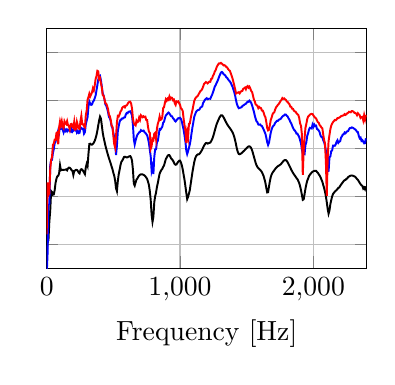
\begin{tikzpicture}

\begin{axis}[%
width=1.6in,
height=1.2in,
at={(1.011in,0.642in)},
scale only axis,
xmin=0,
xmax=2400,
xmajorgrids,
ymin=-30,
ymax=70,
ymajorgrids,
yticklabels={\empty},
xlabel={Frequency [Hz]},
axis background/.style={fill=white}
]
\addplot [color=black,solid,line width=0.7pt,forget plot]
  table[row sep=crcr]{%
0	-24.0683456294169\\
6.66944096884746	-19.3396560250162\\
13.3388819376949	-18.2831164389234\\
20.0083229065424	-10.6084546004752\\
26.6777638753898	-5.97086599305024\\
33.3472048442373	2.16522108527114\\
40.0166458130848	1.75978395548184\\
46.6860867819322	0.626734426887425\\
53.3555277507797	0.737871732712977\\
60.0249687196271	2.52580920909833\\
66.6944096884746	5.58384561111023\\
73.363850657322	7.31560850076007\\
80.0332916261695	8.28717488787875\\
86.702732595017	8.53458853640431\\
93.3721735638644	9.53756253011135\\
100.041614532712	12.9013120736345\\
106.711055501559	10.7979139982812\\
113.380496470407	11.0003823416785\\
120.049937439254	10.9780806423727\\
126.719378408102	10.9337028790663\\
133.388819376949	11.0293859367106\\
140.058260345797	11.047965808486\\
146.727701314644	11.207884167114\\
153.397142283492	10.811670188836\\
160.066583252339	11.6047060753359\\
166.736024221186	11.9228854722147\\
173.405465190034	11.8423295307\\
180.074906158881	11.4786001351701\\
186.744347127729	10.8494779769052\\
193.413788096576	10.6124382924425\\
200.083229065424	8.85277118893201\\
206.752670034271	10.4791231416709\\
213.422111003119	10.7219353557132\\
220.091551971966	10.9741532830638\\
226.760992940814	10.9318703085143\\
233.430433909661	10.5401137397412\\
240.099874878509	9.8403211211292\\
246.769315847356	9.52989652784138\\
253.438756816203	10.9252535590259\\
260.108197785051	11.2714322832669\\
266.777638753898	11.10362079112\\
273.447079722746	10.535687170414\\
280.116520691593	9.84353137333678\\
286.785961660441	9.19822968151163\\
293.455402629288	12.0050357890791\\
300.124843598136	13.508036071824\\
306.794284566983	12.5634588195045\\
313.463725535831	17.7429498864174\\
320.133166504678	21.7758523662437\\
326.802607473525	21.8827559169661\\
333.472048442373	21.5420476915608\\
340.14148941122	21.5103447146577\\
346.810930380068	21.8246620255383\\
353.480371348915	22.2805595788832\\
360.149812317763	23.0438373278984\\
366.81925328661	24.1173060028182\\
373.488694255458	25.5034646941833\\
380.158135224305	27.2972990140191\\
386.827576193153	29.5291205075001\\
393.497017162	31.5804642104892\\
400.166458130848	33.1572120012543\\
406.835899099695	32.3696421680129\\
413.505340068542	29.5545636680595\\
420.17478103739	26.5716681837446\\
426.844222006237	24.4743369392648\\
433.513662975085	22.8761042261215\\
440.183103943932	21.1975168746404\\
446.85254491278	19.7646803934127\\
453.521985881627	18.3912525261677\\
460.191426850475	17.1150417497478\\
466.860867819322	15.8613941539148\\
473.53030878817	14.7319534021528\\
480.199749757017	13.6330447931166\\
486.869190725864	12.4023855514383\\
493.538631694712	11.2701105981622\\
500.208072663559	9.73093014856175\\
506.877513632407	8.51238656479055\\
513.546954601254	6.43515680180294\\
520.216395570102	3.31214094113405\\
526.885836538949	2.12259899988939\\
533.555277507797	6.23921061469215\\
540.224718476644	9.13539560334628\\
546.894159445492	10.9613941129992\\
553.563600414339	12.9188865960616\\
560.233041383186	14.3455417998038\\
566.902482352034	14.8578585252119\\
573.571923320881	15.5662832695366\\
580.241364289729	16.3605108836842\\
586.910805258576	16.4454862922962\\
593.580246227424	16.2963266917826\\
600.249687196271	16.1706099699316\\
606.919128165119	16.2232513492745\\
613.588569133966	16.4692267468046\\
620.258010102814	16.6272386245606\\
626.927451071661	16.7104016795028\\
633.596892040508	16.0914960608922\\
640.266333009356	14.7927641454851\\
646.935773978203	11.0492734021298\\
653.605214947051	5.26770477348501\\
660.274655915898	4.42328522552852\\
666.944096884746	5.74167999892836\\
673.613537853593	6.92559990486053\\
680.282978822441	7.39460929893661\\
686.952419791288	8.11725785269625\\
693.621860760136	8.59932705332204\\
700.291301728983	8.9774021269981\\
706.960742697831	9.10522740949188\\
713.630183666678	9.1353037396175\\
720.299624635525	9.07135800679159\\
726.969065604373	8.8789949439744\\
733.63850657322	8.67846519276452\\
740.307947542068	8.26319748901945\\
746.977388510915	7.77080235551455\\
753.646829479763	7.17215251213036\\
760.31627044861	6.00929245416022\\
766.985711417458	4.63553531744646\\
773.655152386305	2.00836626134394\\
780.324593355153	-1.57423621704266\\
786.994034324	-7.71642217744768\\
793.663475292847	-10.6815049185939\\
800.332916261695	-8.56407760623141\\
807.002357230542	-2.56836154079388\\
813.67179819939	0.0352306843304136\\
820.341239168237	1.53895393047731\\
827.010680137085	3.86571496896091\\
833.680121105932	5.54180740008987\\
840.34956207478	7.51924059516621\\
847.019003043627	9.37657769693219\\
853.688444012475	10.2548611477835\\
860.357884981322	10.9645929524784\\
867.02732595017	11.3483624227316\\
873.696766919017	12.2313202682012\\
880.366207887864	12.8376890056583\\
887.035648856712	14.1765009037456\\
893.705089825559	15.5020787493837\\
900.374530794407	16.126021650216\\
907.043971763254	16.8486066261604\\
913.713412732102	17.151427605075\\
920.382853700949	17.1043887784423\\
927.052294669797	16.475193137847\\
933.721735638644	15.6960885778609\\
940.391176607492	15.3401096983791\\
947.060617576339	14.8872755859658\\
953.730058545186	14.1345016046415\\
960.399499514034	13.3402870476047\\
967.068940482881	13.1218747755534\\
973.738381451729	13.2358423184763\\
980.407822420576	13.8800918961314\\
987.077263389424	14.4137775356716\\
993.746704358271	14.8028618900794\\
1000.41614532712	14.8444961813188\\
1007.08558629597	14.0536551587906\\
1013.75502726481	12.8616725644067\\
1020.42446823366	11.1393378019428\\
1027.09390920251	8.92148884148724\\
1033.76335017136	6.85924025503196\\
1040.4327911402	4.18835541670093\\
1047.10223210905	1.39447568774972\\
1053.7716730779	-1.2048256378795\\
1060.44111404675	-0.305522383453654\\
1067.11055501559	1.1602901793384\\
1073.77999598444	2.64818916328802\\
1080.44943695329	5.20979324519787\\
1087.11887792214	7.70421195966945\\
1093.78831889098	10.223083650422\\
1100.45775985983	12.3243413612199\\
1107.12720082868	14.3020917204378\\
1113.79664179753	15.797438000086\\
1120.46608276637	16.6546771275701\\
1127.13552373522	17.1714901935604\\
1133.80496470407	17.4178883622902\\
1140.47440567292	17.4426645616284\\
1147.14384664176	17.7077802999756\\
1153.81328761061	18.2617759772195\\
1160.48272857946	18.8368287386001\\
1167.15216954831	19.5177515798278\\
1173.82161051715	20.3227244357708\\
1180.491051486	21.0824905700841\\
1187.16049245485	21.678966585198\\
1193.82993342369	22.134930785702\\
1200.49937439254	22.1951602121321\\
1207.16881536139	21.9240722166729\\
1213.83825633024	22.0972639696812\\
1220.50769729908	22.2121942250277\\
1227.17713826793	22.3388264821277\\
1233.84657923678	22.969734682941\\
1240.51602020563	23.6876637556985\\
1247.18546117447	24.6663767020127\\
1253.85490214332	25.8991250151124\\
1260.52434311217	27.2764565737375\\
1267.19378408102	28.631823783618\\
1273.86322504986	29.8698087055702\\
1280.53266601871	30.8325891513041\\
1287.20210698756	31.7022411292012\\
1293.87154795641	32.5247996324368\\
1300.54098892525	33.2178174225289\\
1307.2104298941	33.6986594917876\\
1313.87987086295	33.7421796453155\\
1320.5493118318	33.4375766149507\\
1327.21875280064	32.823010671716\\
1333.88819376949	32.1167366015758\\
1340.55763473834	31.3387688188677\\
1347.22707570719	30.6268857796322\\
1353.89651667603	29.9750499635108\\
1360.56595764488	29.3689327175748\\
1367.23539861373	28.8722193072664\\
1373.90483958258	28.3602746582029\\
1380.57428055142	27.8535472217929\\
1387.24372152027	27.2625172436607\\
1393.91316248912	26.6180483979003\\
1400.58260345797	25.7450870071069\\
1407.25204442681	24.6288727437394\\
1413.92148539566	23.1730477253143\\
1420.59092636451	21.4309604498289\\
1427.26036733336	19.64371591154\\
1433.9298083022	18.3706272081303\\
1440.59924927105	17.623885497496\\
1447.2686902399	17.4924024322815\\
1453.93813120875	17.6566929661315\\
1460.60757217759	17.908822823062\\
1467.27701314644	18.2812242657386\\
1473.94645411529	18.6052888567986\\
1480.61589508414	18.929121906392\\
1487.28533605298	19.3185414898381\\
1493.95477702183	19.7276408819656\\
1500.62421799068	20.0891486547815\\
1507.29365895953	20.4797156807601\\
1513.96309992837	20.7366340459161\\
1520.63254089722	20.7789023642338\\
1527.30198186607	20.5665630077219\\
1533.97142283492	20.0394916342545\\
1540.64086380376	19.1103819735857\\
1547.31030477261	17.8843483383838\\
1553.97974574146	16.5389402258057\\
1560.64918671031	15.2118727027992\\
1567.31862767915	13.8895703938719\\
1573.988068648	12.8956914712557\\
1580.65750961685	12.1861819609547\\
1587.32695058569	11.7127621712836\\
1593.99639155454	11.3331378718527\\
1600.66583252339	11.0334425520856\\
1607.33527349224	10.5725585210773\\
1614.00471446108	10.0437564579848\\
1620.67415542993	9.26559978243927\\
1627.34359639878	8.32537624543794\\
1634.01303736763	7.01788099663447\\
1640.68247833647	5.51226936965034\\
1647.35191930532	3.43388746225421\\
1654.02136027417	1.59259656161962\\
1660.69080124302	1.6769610705975\\
1667.36024221186	4.07671707684635\\
1674.02968318071	6.26723570660015\\
1680.69912414956	7.98015132915848\\
1687.36856511841	9.06972718255109\\
1694.03800608725	9.82304409556608\\
1700.7074470561	10.3265010288481\\
1707.37688802495	10.8286811335363\\
1714.0463289938	11.3594311213406\\
1720.71576996264	11.8353891901172\\
1727.38521093149	12.2232592999122\\
1734.05465190034	12.5159270947538\\
1740.72409286919	12.7333155034326\\
1747.39353383803	12.9447325878673\\
1754.06297480688	13.264726829093\\
1760.73241577573	13.6475208084374\\
1767.40185674458	14.0894725072506\\
1774.07129771342	14.5724274940074\\
1780.74073868227	14.8858656833801\\
1787.41017965112	15.0981995935614\\
1794.07962061997	15.0419807481194\\
1800.74906158881	14.6971167347539\\
1807.41850255766	14.0999371011142\\
1814.08794352651	13.4149912760992\\
1820.75738449536	12.6339137941732\\
1827.4268254642	11.9041773485643\\
1834.09626643305	11.0735691159399\\
1840.7657074019	10.3902465482427\\
1847.43514837075	9.75105508190697\\
1854.10458933959	9.12567499148209\\
1860.77403030844	8.6372645285149\\
1867.44347127729	8.10367168424845\\
1874.11291224614	7.51372353571495\\
1880.78235321498	7.14545112312349\\
1887.45179418383	6.27912177809227\\
1894.12123515268	5.47823090416729\\
1900.79067612153	4.16927543285802\\
1907.46011709037	2.4989710691914\\
1914.12955805922	0.573175775601438\\
1920.79899902807	-1.50252038078113\\
1927.46843999692	-1.28847058933952\\
1934.13788096576	0.820572357951112\\
1940.80732193461	3.1273829499776\\
1947.47676290346	4.96892508262679\\
1954.14620387231	6.42838171758779\\
1960.81564484115	7.38835247709589\\
1967.48508581	8.41043744836154\\
1974.15452677885	8.96166222494187\\
1980.82396774769	9.40938010029019\\
1987.49340871654	9.86093262230319\\
1994.16284968539	10.229591473129\\
2000.83229065424	10.3937650086228\\
2007.50173162308	10.5725125460773\\
2014.17117259193	10.5568690795315\\
2020.84061356078	10.6011693496467\\
2027.51005452963	10.0907245762853\\
2034.17949549847	9.76026970491023\\
2040.84893646732	9.11270086616989\\
2047.51837743617	8.59304568254099\\
2054.18781840502	7.88545415762906\\
2060.85725937386	6.91133000677038\\
2067.52670034271	6.06082099544079\\
2074.19614131156	4.66084729886208\\
2080.86558228041	3.40540971228569\\
2087.53502324925	1.8796640192215\\
2094.2044642181	-0.093741562218218\\
2100.87390518695	-2.52751460968796\\
2107.5433461558	-5.3189079569175\\
2114.21278712464	-7.26363503695163\\
2120.88222809349	-5.95259541067369\\
2127.55166906234	-3.30666876916218\\
2134.22111003119	-1.63516896346401\\
2140.89055100003	-0.0861781487793506\\
2147.55999196888	0.902175900766741\\
2154.22943293773	1.4375430188796\\
2160.89887390658	1.87546391752145\\
2167.56831487542	2.2507200038696\\
2174.23775584427	2.56300321052649\\
2180.90719681312	2.97714173535604\\
2187.57663778197	3.51160690726077\\
2194.24607875081	3.60968157040522\\
2200.91551971966	4.29881125421\\
2207.58496068851	4.81950345222116\\
2214.25440165736	5.32673110885806\\
2220.9238426262	5.83337487484509\\
2227.59328359505	6.32024074003078\\
2234.2627245639	6.68118255995198\\
2240.93216553275	6.7702877226838\\
2247.60160650159	7.25852422501979\\
2254.27104747044	7.38938023552128\\
2260.94048843929	7.9437751479342\\
2267.60992940814	8.22818822535829\\
2274.27937037698	8.44339843748762\\
2280.94881134583	8.58939886313787\\
2287.61825231468	8.64749764088931\\
2294.28769328353	8.6004395201204\\
2300.95713425237	8.45639762915704\\
2307.62657522122	8.26017247578103\\
2314.29601619007	8.08596249513361\\
2320.96545715892	7.64670346143461\\
2327.63489812776	7.12827483486503\\
2334.30433909661	6.82501214882998\\
2340.97378006546	6.206654984171\\
2347.64322103431	5.56909420242175\\
2354.31266200315	5.02450287607549\\
2360.982102972	4.53577485019492\\
2367.65154394085	4.3038407985004\\
2374.3209849097	3.18472608978428\\
2380.99042587854	3.6356088439887\\
2387.65986684739	2.91405044525092\\
2394.32930781624	4.11006441955449\\
};
\addplot [color=blue,solid,line width=0.7pt,forget plot]
  table[row sep=crcr]{%
0	-32.9911030478466\\
6.66944096884746	-23.9493486484162\\
13.3388819376949	-3.72523897701383\\
20.0083229065424	-3.19289825523262\\
26.6777638753898	12.8882470600692\\
33.3472048442373	14.9944569831076\\
40.0166458130848	15.1694300812681\\
46.6860867819322	17.9730137663397\\
53.3555277507797	19.5640199206439\\
60.0249687196271	22.0985732143736\\
66.6944096884746	22.6342920039143\\
73.363850657322	24.6714582668792\\
80.0332916261695	26.0629546198859\\
86.702732595017	27.4503458346258\\
93.3721735638644	26.4188295814252\\
100.041614532712	29.2137155733383\\
106.711055501559	28.0849581248447\\
113.380496470407	28.1985602805541\\
120.049937439254	27.7582334551671\\
126.719378408102	26.6096294724706\\
133.388819376949	27.9364940511809\\
140.058260345797	27.1845293753886\\
146.727701314644	27.7530104855528\\
153.397142283492	27.0471842527131\\
160.066583252339	27.7209276150668\\
166.736024221186	27.3997872162661\\
173.405465190034	27.0949418276849\\
180.074906158881	26.9333520609288\\
186.744347127729	28.1782591900881\\
193.413788096576	26.9084006642643\\
200.083229065424	27.3048280358573\\
206.752670034271	28.0521528381798\\
213.422111003119	27.5352663504472\\
220.091551971966	27.9532035495036\\
226.760992940814	26.5253066858007\\
233.430433909661	27.1147728597767\\
240.099874878509	26.3096670834537\\
246.769315847356	26.4417185313727\\
253.438756816203	28.7192051588625\\
260.108197785051	28.3403275776518\\
266.777638753898	28.0740269640985\\
273.447079722746	28.1754920514789\\
280.116520691593	26.0565625012168\\
286.785961660441	26.7032861171474\\
293.455402629288	29.9756181547953\\
300.124843598136	31.4802025053901\\
306.794284566983	32.9471783092666\\
313.463725535831	37.4707926829378\\
320.133166504678	39.4638650656014\\
326.802607473525	38.461425643527\\
333.472048442373	38.0350060686982\\
340.14148941122	38.2390812340478\\
346.810930380068	39.3652259902431\\
353.480371348915	39.7772890985887\\
360.149812317763	40.7900509895623\\
366.81925328661	41.8943043425619\\
373.488694255458	44.1264986042707\\
380.158135224305	46.2424622743115\\
386.827576193153	48.610620848918\\
393.497017162	49.7263901739566\\
400.166458130848	50.0881391358802\\
406.835899099695	48.2145704609459\\
413.505340068542	45.7554513445466\\
420.17478103739	42.8837014883868\\
426.844222006237	42.0313099017071\\
433.513662975085	40.3563793224918\\
440.183103943932	38.2867897398727\\
446.85254491278	37.6971096084161\\
453.521985881627	36.5252015227653\\
460.191426850475	35.0582037009402\\
466.860867819322	33.0893171857907\\
473.53030878817	32.4888973958971\\
480.199749757017	31.3043499793293\\
486.869190725864	29.2423862343193\\
493.538631694712	28.4820981264918\\
500.208072663559	26.3362971636329\\
506.877513632407	24.4846607866333\\
513.546954601254	21.821024930961\\
520.216395570102	17.1895833290287\\
526.885836538949	21.0524152620515\\
533.555277507797	27.0972301604211\\
540.224718476644	29.1612182562142\\
546.894159445492	30.9711260563439\\
553.563600414339	31.905068242585\\
560.233041383186	31.9395576120532\\
566.902482352034	32.453785743734\\
573.571923320881	32.4363154070259\\
580.241364289729	32.819735489049\\
586.910805258576	32.8683749100292\\
593.580246227424	34.046961775724\\
600.249687196271	34.6638406675935\\
606.919128165119	34.5647660621537\\
613.588569133966	35.1970156984553\\
620.258010102814	35.2756173439307\\
626.927451071661	35.3657773128636\\
633.596892040508	34.644786458341\\
640.266333009356	33.5564661404354\\
646.935773978203	29.6300491447957\\
653.605214947051	23.6681275051683\\
660.274655915898	21.5753665402143\\
666.944096884746	23.214144723642\\
673.613537853593	24.5800492840334\\
680.282978822441	25.6321307822314\\
686.952419791288	26.0438328202817\\
693.621860760136	26.6233311081754\\
700.291301728983	26.7828651645445\\
706.960742697831	27.5424287390197\\
713.630183666678	27.2337772155476\\
720.299624635525	27.2029707393368\\
726.969065604373	27.3404966683015\\
733.63850657322	26.6657416979935\\
740.307947542068	26.3732775695923\\
746.977388510915	25.9089991313797\\
753.646829479763	25.3349165475415\\
760.31627044861	23.9430929534186\\
766.985711417458	22.1365823771762\\
773.655152386305	19.3577515933716\\
780.324593355153	16.53998175632\\
786.994034324	10.6447183979001\\
793.663475292847	12.2746883618553\\
800.332916261695	9.21113461217376\\
807.002357230542	16.3407504019938\\
813.67179819939	19.5058694191803\\
820.341239168237	19.5904646964221\\
827.010680137085	22.4537588589258\\
833.680121105932	23.0978538553613\\
840.34956207478	25.4400631147836\\
847.019003043627	27.9513900920438\\
853.688444012475	27.7579961850178\\
860.357884981322	28.3666841827425\\
867.02732595017	28.9508400658904\\
873.696766919017	30.6270828476855\\
880.366207887864	31.0641679247894\\
887.035648856712	32.5669647872601\\
893.705089825559	33.661264688455\\
900.374530794407	34.004053302836\\
907.043971763254	34.5723777518559\\
913.713412732102	34.8671470040605\\
920.382853700949	34.4779373999857\\
927.052294669797	33.878897904307\\
933.721735638644	33.3680928800445\\
940.391176607492	33.2794457113412\\
947.060617576339	32.5528911133938\\
953.730058545186	32.1705253232438\\
960.399499514034	31.4586501893057\\
967.068940482881	31.1542197533857\\
973.738381451729	31.6430621504102\\
980.407822420576	32.1360116296428\\
987.077263389424	32.5173466388437\\
993.746704358271	32.4596004192773\\
1000.41614532712	32.6842365961747\\
1007.08558629597	32.1892967972253\\
1013.75502726481	31.0885190374921\\
1020.42446823366	29.3698810031473\\
1027.09390920251	27.71269089098\\
1033.76335017136	25.3361484353639\\
1040.4327911402	22.8342240369941\\
1047.10223210905	19.0409817030887\\
1053.7716730779	17.5700738929698\\
1060.44111404675	18.7567019380581\\
1067.11055501559	20.2118990573233\\
1073.77999598444	21.6444504437169\\
1080.44943695329	23.8226243579601\\
1087.11887792214	26.4571664171698\\
1093.78831889098	28.8923060357469\\
1100.45775985983	30.9694101045343\\
1107.12720082868	33.1652951631983\\
1113.79664179753	34.1727915316714\\
1120.46608276637	35.1453579590845\\
1127.13552373522	35.6034354329524\\
1133.80496470407	35.8978015184113\\
1140.47440567292	35.9220775109852\\
1147.14384664176	36.2306602190339\\
1153.81328761061	36.9722127981744\\
1160.48272857946	37.1395314484115\\
1167.15216954831	37.5570011040245\\
1173.82161051715	38.9393669103552\\
1180.491051486	39.5154430369553\\
1187.16049245485	40.2243305010845\\
1193.82993342369	40.5882664373719\\
1200.49937439254	40.8568303052708\\
1207.16881536139	40.4310464564403\\
1213.83825633024	40.5939783687801\\
1220.50769729908	40.6193742093799\\
1227.17713826793	40.5993037088439\\
1233.84657923678	41.5151888028314\\
1240.51602020563	42.2410206105889\\
1247.18546117447	43.2881811309055\\
1253.85490214332	44.4137290240183\\
1260.52434311217	45.6358898647127\\
1267.19378408102	46.2697135483571\\
1273.86322504986	47.133671125369\\
1280.53266601871	47.8930963080804\\
1287.20210698756	48.8179797531643\\
1293.87154795641	49.8610192775318\\
1300.54098892525	50.7189480289263\\
1307.2104298941	51.5502877404391\\
1313.87987086295	51.7787047987723\\
1320.5493118318	51.4520594934599\\
1327.21875280064	50.7972843673287\\
1333.88819376949	50.593181327684\\
1340.55763473834	50.2142455343601\\
1347.22707570719	49.5646263205704\\
1353.89651667603	49.3232152346369\\
1360.56595764488	48.6706181150399\\
1367.23539861373	48.2562198576883\\
1373.90483958258	47.8228898878867\\
1380.57428055142	47.227794890676\\
1387.24372152027	46.3776829544659\\
1393.91316248912	45.6505835715468\\
1400.58260345797	44.4169873853863\\
1407.25204442681	43.3371643763984\\
1413.92148539566	41.7518111808162\\
1420.59092636451	39.8649486193219\\
1427.26036733336	38.3111547952827\\
1433.9298083022	37.3896353309573\\
1440.59924927105	36.6811052920655\\
1447.2686902399	36.779035440207\\
1453.93813120875	36.9552681939327\\
1460.60757217759	37.0402049884432\\
1467.27701314644	37.5314531426594\\
1473.94645411529	37.8121634165881\\
1480.61589508414	38.0590836802344\\
1487.28533605298	38.3349371062933\\
1493.95477702183	38.5266182289995\\
1500.62421799068	38.9879853862921\\
1507.29365895953	39.4235774328029\\
1513.96309992837	39.3520609984238\\
1520.63254089722	39.8401456696655\\
1527.30198186607	39.5032966447556\\
1533.97142283492	38.8823024543383\\
1540.64086380376	37.8387874158946\\
1547.31030477261	36.5364730971605\\
1553.97974574146	35.2998597215208\\
1560.64918671031	33.6410205443619\\
1567.31862767915	32.3160663351958\\
1573.988068648	31.2016577897609\\
1580.65750961685	30.8203756704131\\
1587.32695058569	29.8656706258846\\
1593.99639155454	29.8104617943048\\
1600.66583252339	29.9243412324825\\
1607.33527349224	29.453583408413\\
1614.00471446108	29.2568415375585\\
1620.67415542993	28.580850215712\\
1627.34359639878	27.7581603224422\\
1634.01303736763	26.8951108246436\\
1640.68247833647	25.9761632133234\\
1647.35191930532	24.3797469274777\\
1654.02136027417	22.4760753168022\\
1660.69080124302	21.3469728227262\\
1667.36024221186	22.2989972999103\\
1674.02968318071	24.4315568230609\\
1680.69912414956	26.4991595393359\\
1687.36856511841	27.9215460431871\\
1694.03800608725	28.8759079171232\\
1700.7074470561	29.3545996828021\\
1707.37688802495	29.7518352254451\\
1714.0463289938	30.6052455652818\\
1720.71576996264	31.0062090726134\\
1727.38521093149	31.4322876713654\\
1734.05465190034	31.4301600244413\\
1740.72409286919	31.859819909352\\
1747.39353383803	32.0221776696462\\
1754.06297480688	32.1919285341958\\
1760.73241577573	32.6545067755328\\
1767.40185674458	33.2069259783595\\
1774.07129771342	33.5182881741092\\
1780.74073868227	33.6698736442814\\
1787.41017965112	34.0658808588037\\
1794.07962061997	33.9955147426232\\
1800.74906158881	33.521859111515\\
1807.41850255766	33.2214597282048\\
1814.08794352651	32.4127555730694\\
1820.75738449536	31.8876078948596\\
1827.4268254642	30.9586199652516\\
1834.09626643305	30.3815156587638\\
1840.7657074019	29.4021708621147\\
1847.43514837075	28.5309525555571\\
1854.10458933959	27.7706146154678\\
1860.77403030844	27.4316528732188\\
1867.44347127729	26.8503417334896\\
1874.11291224614	26.0367420707288\\
1880.78235321498	26.0590707858897\\
1887.45179418383	25.3671478407102\\
1894.12123515268	24.6654724845114\\
1900.79067612153	23.3114799728597\\
1907.46011709037	22.0179866204812\\
1914.12955805922	19.3961291496787\\
1920.79899902807	17.8022276527788\\
1927.46843999692	17.6548731983709\\
1934.13788096576	17.5035959865795\\
1940.80732193461	21.3660874822244\\
1947.47676290346	22.4947333536285\\
1954.14620387231	25.1617612406456\\
1960.81564484115	26.2592178396819\\
1967.48508581	27.7716643970098\\
1974.15452677885	28.5106748846076\\
1980.82396774769	28.4170565254726\\
1987.49340871654	28.2388744661988\\
1994.16284968539	29.8472100077911\\
2000.83229065424	28.9759565261388\\
2007.50173162308	29.8723643083152\\
2014.17117259193	29.2781595109124\\
2020.84061356078	29.39011786839\\
2027.51005452963	27.9988971309743\\
2034.17949549847	27.8017603333607\\
2040.84893646732	27.3918503831745\\
2047.51837743617	26.6066711646369\\
2054.18781840502	25.2273648412503\\
2060.85725937386	24.6574339747827\\
2067.52670034271	24.6024881037742\\
2074.19614131156	23.3387617043142\\
2080.86558228041	22.494141674364\\
2087.53502324925	21.0509976970559\\
2094.2044642181	18.9620726181707\\
2100.87390518695	17.7194369146482\\
2107.5433461558	15.6320913323561\\
2114.21278712464	10.2243000052608\\
2120.88222809349	16.181179288116\\
2127.55166906234	16.5829989391791\\
2134.22111003119	18.8024346510015\\
2140.89055100003	19.0794620256377\\
2147.55999196888	21.0651859772837\\
2154.22943293773	21.0664117551235\\
2160.89887390658	21.0172950094865\\
2167.56831487542	21.5624940433568\\
2174.23775584427	22.6714524740408\\
2180.90719681312	23.3009332717732\\
2187.57663778197	22.2624629080647\\
2194.24607875081	22.7546370785866\\
2200.91551971966	22.9075055749883\\
2207.58496068851	24.4032929604458\\
2214.25440165736	24.9364091840332\\
2220.9238426262	25.7139083318887\\
2227.59328359505	25.8079803816047\\
2234.2627245639	26.5394551936622\\
2240.93216553275	26.2380526010817\\
2247.60160650159	26.6690741280082\\
2254.27104747044	27.0280047799649\\
2260.94048843929	27.1435883058789\\
2267.60992940814	27.9460482614936\\
2274.27937037698	28.399105794435\\
2280.94881134583	28.3683554745598\\
2287.61825231468	28.6728363494274\\
2294.28769328353	28.5742207670517\\
2300.95713425237	28.3509254079886\\
2307.62657522122	28.065645574148\\
2314.29601619007	27.862607238926\\
2320.96545715892	27.4368795700435\\
2327.63489812776	26.8454673624891\\
2334.30433909661	26.6885925200608\\
2340.97378006546	25.1159046121839\\
2347.64322103431	24.1151873660673\\
2354.31266200315	24.4066643632383\\
2360.982102972	23.0696318989832\\
2367.65154394085	23.3716268990633\\
2374.3209849097	22.7595675486665\\
2380.99042587854	22.0261855607901\\
2387.65986684739	22.1248104490739\\
2394.32930781624	24.1371540911869\\
};
\addplot [color=red,solid,line width=0.7pt,forget plot]
  table[row sep=crcr]{%
0	-15.9166573722451\\
6.66944096884746	5.7727813272995\\
13.3388819376949	0.466534529039145\\
20.0083229065424	1.17288697208377\\
26.6777638753898	11.1129236834485\\
33.3472048442373	15.1503828337624\\
40.0166458130848	16.3199225743641\\
46.6860867819322	21.3775663194375\\
53.3555277507797	21.9423254388088\\
60.0249687196271	23.5766489076422\\
66.6944096884746	23.5261034626579\\
73.363850657322	26.3290196300707\\
80.0332916261695	26.6213288590569\\
86.702732595017	21.6809043462437\\
93.3721735638644	28.7686096602393\\
100.041614532712	31.1586959876368\\
106.711055501559	29.5615468148337\\
113.380496470407	31.2383803261885\\
120.049937439254	28.9824657624264\\
126.719378408102	28.3578707927252\\
133.388819376949	31.2662025630493\\
140.058260345797	30.4734271972439\\
146.727701314644	30.0347650146248\\
153.397142283492	31.2731269452646\\
160.066583252339	29.5898851155533\\
166.736024221186	29.2602748914655\\
173.405465190034	27.8072448686016\\
180.074906158881	30.0077122729223\\
186.744347127729	30.1428494948326\\
193.413788096576	28.9294615719928\\
200.083229065424	28.5316442585842\\
206.752670034271	31.030592768106\\
213.422111003119	27.7427884843708\\
220.091551971966	27.8694157345634\\
226.760992940814	30.971458309854\\
233.430433909661	29.5282105052846\\
240.099874878509	28.2046200649523\\
246.769315847356	28.0408193032272\\
253.438756816203	31.2497467958431\\
260.108197785051	33.4456487131798\\
266.777638753898	29.9755634635663\\
273.447079722746	29.9586243668849\\
280.116520691593	29.2067488749606\\
286.785961660441	28.7631264476492\\
293.455402629288	33.7392566899634\\
300.124843598136	35.6779839491419\\
306.794284566983	40.2391843769685\\
313.463725535831	41.2884258343493\\
320.133166504678	42.72068137403\\
326.802607473525	41.606997436853\\
333.472048442373	42.4281769381846\\
340.14148941122	43.3005538150799\\
346.810930380068	44.9838185210262\\
353.480371348915	44.1215346511421\\
360.149812317763	46.0150249845228\\
366.81925328661	48.7789723256093\\
373.488694255458	50.005559527456\\
380.158135224305	52.2411758818896\\
386.827576193153	52.0187920813396\\
393.497017162	48.7351056881592\\
400.166458130848	49.200126260709\\
406.835899099695	47.0950234036378\\
413.505340068542	45.3246964755478\\
420.17478103739	42.2290455231076\\
426.844222006237	41.8523588871947\\
433.513662975085	40.4495292050155\\
440.183103943932	38.8072690809847\\
446.85254491278	38.5427280517593\\
453.521985881627	37.6305572186427\\
460.191426850475	36.3297434012287\\
466.860867819322	34.010446122615\\
473.53030878817	33.3583817998223\\
480.199749757017	31.942920444297\\
486.869190725864	29.4556645278944\\
493.538631694712	29.0115149473677\\
500.208072663559	24.9739921229138\\
506.877513632407	21.618306240427\\
513.546954601254	20.2824934637897\\
520.216395570102	25.0565491769448\\
526.885836538949	30.8122827961153\\
533.555277507797	33.4452481467853\\
540.224718476644	33.2369571925232\\
546.894159445492	34.0902453505908\\
553.563600414339	35.2828593298327\\
560.233041383186	35.7664014949452\\
566.902482352034	36.9080457557325\\
573.571923320881	37.244917847718\\
580.241364289729	37.4450710137922\\
586.910805258576	37.0393864560293\\
593.580246227424	37.7092596195648\\
600.249687196271	37.872160662078\\
606.919128165119	38.4242142429194\\
613.588569133966	39.0641019684289\\
620.258010102814	39.3406293732703\\
626.927451071661	39.3963862454045\\
633.596892040508	38.547868505605\\
640.266333009356	36.4739920353756\\
646.935773978203	32.3319479041048\\
653.605214947051	30.4478959399044\\
660.274655915898	29.8330260509554\\
666.944096884746	29.4931921673778\\
673.613537853593	31.507425167128\\
680.282978822441	30.8490722008588\\
686.952419791288	31.0930865762581\\
693.621860760136	32.7741277482998\\
700.291301728983	31.8891770960268\\
706.960742697831	33.7005576040885\\
713.630183666678	33.2184726291818\\
720.299624635525	32.8887399060044\\
726.969065604373	33.3286485975053\\
733.63850657322	32.9623636123547\\
740.307947542068	33.1232890434278\\
746.977388510915	31.7385086093281\\
753.646829479763	31.717819762229\\
760.31627044861	28.7280839673643\\
766.985711417458	26.8912409801611\\
773.655152386305	26.3793835758003\\
780.324593355153	19.7554655888476\\
786.994034324	20.8035019881163\\
793.663475292847	23.7806459241728\\
800.332916261695	23.3760451387054\\
807.002357230542	26.0769204398401\\
813.67179819939	26.4306749876943\\
820.341239168237	23.7596418564485\\
827.010680137085	28.2062943473763\\
833.680121105932	30.2173042770468\\
840.34956207478	31.4060912240434\\
847.019003043627	33.2516309727859\\
853.688444012475	31.8129526563048\\
860.357884981322	31.9913812235353\\
867.02732595017	32.9453294481753\\
873.696766919017	36.6846513309377\\
880.366207887864	37.1163496012141\\
887.035648856712	38.9969048237119\\
893.705089825559	40.4146467061526\\
900.374530794407	39.8089187720894\\
907.043971763254	40.658708064057\\
913.713412732102	40.2452500851809\\
920.382853700949	41.5655475753753\\
927.052294669797	40.526122313212\\
933.721735638644	41.1072423997775\\
940.391176607492	41.0236635348041\\
947.060617576339	40.0207457908081\\
953.730058545186	40.2690876304875\\
960.399499514034	38.7924806730847\\
967.068940482881	38.0730712011086\\
973.738381451729	39.4976981478749\\
980.407822420576	39.268557626061\\
987.077263389424	39.5236329490998\\
993.746704358271	38.7148680050669\\
1000.41614532712	38.074381557185\\
1007.08558629597	36.5688804334082\\
1013.75502726481	36.2892348369117\\
1020.42446823366	35.558442234763\\
1027.09390920251	32.2723584642644\\
1033.76335017136	29.6071736678742\\
1040.4327911402	27.4575865297252\\
1047.10223210905	22.1364530728529\\
1053.7716730779	26.5578226327586\\
1060.44111404675	24.4502784286066\\
1067.11055501559	30.1912549782007\\
1073.77999598444	30.2879122685375\\
1080.44943695329	32.5684564328458\\
1087.11887792214	34.4410173506056\\
1093.78831889098	35.9858354656893\\
1100.45775985983	37.9481822103353\\
1107.12720082868	39.7377779685575\\
1113.79664179753	40.6479868571083\\
1120.46608276637	41.2003663783062\\
1127.13552373522	41.5248027514698\\
1133.80496470407	41.8378150974417\\
1140.47440567292	42.5738888080605\\
1147.14384664176	43.2283722989636\\
1153.81328761061	43.8984216443765\\
1160.48272857946	44.0841878935522\\
1167.15216954831	44.7602720121795\\
1173.82161051715	45.7409957826869\\
1180.491051486	46.756004333924\\
1187.16049245485	47.116494263387\\
1193.82993342369	47.5636238108654\\
1200.49937439254	47.399598995824\\
1207.16881536139	46.998148161962\\
1213.83825633024	47.3672947309026\\
1220.50769729908	47.7456843544464\\
1227.17713826793	47.6978578953439\\
1233.84657923678	48.8832876125163\\
1240.51602020563	49.0293608729749\\
1247.18546117447	50.2184480993194\\
1253.85490214332	50.793500754851\\
1260.52434311217	51.9435684201216\\
1267.19378408102	52.5139459278957\\
1273.86322504986	53.6200689097834\\
1280.53266601871	54.3967028494662\\
1287.20210698756	54.9947698105518\\
1293.87154795641	55.383785068077\\
1300.54098892525	55.2899831995579\\
1307.2104298941	55.5454641704128\\
1313.87987086295	55.2328762921881\\
1320.5493118318	54.9217216891353\\
1327.21875280064	54.499188146447\\
1333.88819376949	54.5975469401634\\
1340.55763473834	54.3250880821505\\
1347.22707570719	53.8447821959367\\
1353.89651667603	53.6685860506419\\
1360.56595764488	52.9900768427304\\
1367.23539861373	52.5353653245925\\
1373.90483958258	52.2523685877237\\
1380.57428055142	51.2416473086961\\
1387.24372152027	50.2148897159114\\
1393.91316248912	49.0387471510784\\
1400.58260345797	47.5371846504938\\
1407.25204442681	46.0657474332827\\
1413.92148539566	44.4783632058311\\
1420.59092636451	42.7902776925993\\
1427.26036733336	43.1123200450165\\
1433.9298083022	43.169253771305\\
1440.59924927105	43.3126501480482\\
1447.2686902399	42.8450963567795\\
1453.93813120875	43.4463759616296\\
1460.60757217759	43.7729733162887\\
1467.27701314644	43.8526421249546\\
1473.94645411529	44.7420187442288\\
1480.61589508414	44.9690847892904\\
1487.28533605298	45.2634671256524\\
1493.95477702183	44.5608358058988\\
1500.62421799068	45.5941063211602\\
1507.29365895953	45.8998808837005\\
1513.96309992837	45.2487090991298\\
1520.63254089722	45.6717920936109\\
1527.30198186607	44.876035305562\\
1533.97142283492	43.8329455553913\\
1540.64086380376	43.4293002235256\\
1547.31030477261	41.9367503728009\\
1553.97974574146	40.3379220566533\\
1560.64918671031	39.5832495957682\\
1567.31862767915	38.233304006273\\
1573.988068648	38.0174514010656\\
1580.65750961685	37.581636908543\\
1587.32695058569	36.6900066539402\\
1593.99639155454	37.1982074870999\\
1600.66583252339	36.8444855870193\\
1607.33527349224	36.706999030775\\
1614.00471446108	35.7211275890694\\
1620.67415542993	35.6563713529236\\
1627.34359639878	34.8380023631553\\
1634.01303736763	33.5680502906775\\
1640.68247833647	32.9095792325915\\
1647.35191930532	30.8756738257373\\
1654.02136027417	28.4393505733653\\
1660.69080124302	27.4233160008823\\
1667.36024221186	27.6795065296431\\
1674.02968318071	29.6544914438187\\
1680.69912414956	31.7986650753864\\
1687.36856511841	32.7864281084789\\
1694.03800608725	34.1432797370737\\
1700.7074470561	34.7175601619291\\
1707.37688802495	35.0227643375301\\
1714.0463289938	36.1989957143977\\
1720.71576996264	37.0640271485471\\
1727.38521093149	37.4828872336955\\
1734.05465190034	38.0949589212358\\
1740.72409286919	38.457030881487\\
1747.39353383803	39.003947397611\\
1754.06297480688	39.6821554827284\\
1760.73241577573	40.1385636478451\\
1767.40185674458	40.9009356821525\\
1774.07129771342	40.5583081904966\\
1780.74073868227	40.7532558761015\\
1787.41017965112	40.3822665627404\\
1794.07962061997	40.1694035124366\\
1800.74906158881	39.4488007107592\\
1807.41850255766	39.3069726333445\\
1814.08794352651	38.7017246147348\\
1820.75738449536	38.3225313440421\\
1827.4268254642	37.3145760281752\\
1834.09626643305	37.2902182343231\\
1840.7657074019	36.4720975761419\\
1847.43514837075	36.3915476356723\\
1854.10458933959	35.6548144059215\\
1860.77403030844	35.3578125695466\\
1867.44347127729	35.1936440933633\\
1874.11291224614	34.5229777303763\\
1880.78235321498	34.2211443795927\\
1887.45179418383	33.8132681203079\\
1894.12123515268	32.582208751899\\
1900.79067612153	30.3633665249673\\
1907.46011709037	29.3323465392366\\
1914.12955805922	25.7893949723862\\
1920.79899902807	8.86828504621739\\
1927.46843999692	19.18273650786\\
1934.13788096576	24.137963749762\\
1940.80732193461	28.494959681372\\
1947.47676290346	30.110041034501\\
1954.14620387231	32.1431885993566\\
1960.81564484115	33.2287624309593\\
1967.48508581	33.5462833252981\\
1974.15452677885	33.9882285067414\\
1980.82396774769	34.219334000955\\
1987.49340871654	34.308553610117\\
1994.16284968539	34.2359419933984\\
2000.83229065424	33.6480590384476\\
2007.50173162308	33.0513243470575\\
2014.17117259193	32.6537273976895\\
2020.84061356078	32.4165896750737\\
2027.51005452963	31.5070654397663\\
2034.17949549847	30.8234297875194\\
2040.84893646732	30.5872449008564\\
2047.51837743617	29.6005399376585\\
2054.18781840502	29.2712498081404\\
2060.85725937386	28.6172789844209\\
2067.52670034271	28.3111469937525\\
2074.19614131156	25.6806235361496\\
2080.86558228041	23.4188141133583\\
2087.53502324925	21.974284665338\\
2094.2044642181	14.1553715139799\\
2100.87390518695	0.190675794902305\\
2107.5433461558	15.8512813432047\\
2114.21278712464	22.9182629557608\\
2120.88222809349	25.4863079608773\\
2127.55166906234	27.9012580138028\\
2134.22111003119	29.4373386980064\\
2140.89055100003	30.2516910192712\\
2147.55999196888	30.8801446380846\\
2154.22943293773	31.316807090847\\
2160.89887390658	31.7871709933503\\
2167.56831487542	31.6656035839155\\
2174.23775584427	32.0054769951951\\
2180.90719681312	32.5440896999641\\
2187.57663778197	32.5435467847273\\
2194.24607875081	32.8020226959832\\
2200.91551971966	32.9640134612258\\
2207.58496068851	33.3644247376178\\
2214.25440165736	33.4867943628366\\
2220.9238426262	33.6104538607392\\
2227.59328359505	33.7238670324283\\
2234.2627245639	34.2014618698699\\
2240.93216553275	33.8859515986868\\
2247.60160650159	34.1304884510119\\
2254.27104747044	34.5852938084626\\
2260.94048843929	34.7425082240475\\
2267.60992940814	35.1941912079066\\
2274.27937037698	35.1154866949631\\
2280.94881134583	34.9763717757185\\
2287.61825231468	35.4795514455589\\
2294.28769328353	35.4453035067351\\
2300.95713425237	35.2139745306894\\
2307.62657522122	34.7601370090608\\
2314.29601619007	34.705824797878\\
2320.96545715892	34.4154475361369\\
2327.63489812776	33.745220283305\\
2334.30433909661	34.5543937431383\\
2340.97378006546	34.0717549954496\\
2347.64322103431	33.7451709862361\\
2354.31266200315	32.6033056531279\\
2360.982102972	32.9173698090619\\
2367.65154394085	33.0752092324118\\
2374.3209849097	31.5949842477609\\
2380.99042587854	33.7517861483614\\
2387.65986684739	31.9773644125181\\
2394.32930781624	33.9035600914742\\
};
\end{axis}
\end{tikzpicture}%
	\caption{Enclosure tests.}
	\label{fig:freq_responsecomb}
\end{subfigure}
\begin{subfigure}[t]{0.32\textwidth}
	\tikzsetnextfilename{FFT_mic_comb}
	% This file was created by matlab2tikz.
%
%The latest updates can be retrieved from
%  http://www.mathworks.com/matlabcentral/fileexchange/22022-matlab2tikz-matlab2tikz
%where you can also make suggestions and rate matlab2tikz.
%
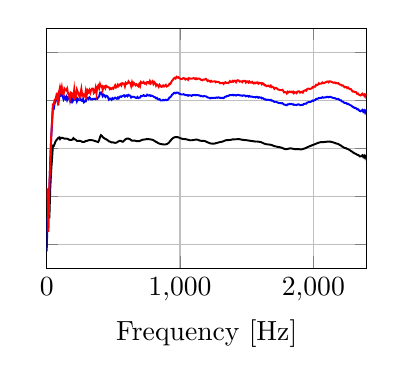
\begin{tikzpicture}

\begin{axis}[%
width=1.6in,
height=1.2in,
at={(1.011in,0.642in)},
scale only axis,
xmin=0,
xmax=2400,
xmajorgrids,
ymin=-30,
ymax=70,
ymajorgrids,
yticklabels={\empty},
xlabel={Frequency [Hz]},
axis background/.style={fill=white},
legend style={legend cell align=left,align=left,draw=white!15!black}
]
\addplot [color=black,solid,line width=0.7pt]
  table[row sep=crcr]{%
0	-7.06319138244352\\
6.66944096884746	-12.1451580312815\\
13.3388819376949	3.16038127446593\\
20.0083229065424	-9.20169992384766\\
26.6777638753898	2.99231449025392\\
33.3472048442373	10.4267536619528\\
40.0166458130848	15.3999184470329\\
46.6860867819322	21.0446548063046\\
53.3555277507797	20.9348892341851\\
60.0249687196271	21.8708533669927\\
66.6944096884746	22.8518234506085\\
73.363850657322	23.3578792470604\\
80.0332916261695	23.8315096670983\\
86.702732595017	24.3089943017668\\
93.3721735638644	24.5063679281205\\
100.041614532712	23.8322664031605\\
106.711055501559	24.3448985900992\\
113.380496470407	24.2763731563769\\
120.049937439254	24.2753569302173\\
126.719378408102	24.1446764899339\\
133.388819376949	23.9878327816752\\
140.058260345797	23.9638239359001\\
146.727701314644	23.9835990674547\\
153.397142283492	23.936499491716\\
160.066583252339	23.8538335978623\\
166.736024221186	23.5865641726001\\
173.405465190034	23.4807777991426\\
180.074906158881	23.4105302027429\\
186.744347127729	23.5131436267766\\
193.413788096576	23.5589188939945\\
200.083229065424	24.1742597778778\\
206.752670034271	23.8071383161221\\
213.422111003119	23.6906719549896\\
220.091551971966	23.3936046288611\\
226.760992940814	23.0786264423957\\
233.430433909661	22.9944680696515\\
240.099874878509	23.0781701951232\\
246.769315847356	23.064198357722\\
253.438756816203	22.9962026800357\\
260.108197785051	22.8479502262225\\
266.777638753898	22.6678448981319\\
273.447079722746	22.6055554645273\\
280.116520691593	22.6052864894416\\
286.785961660441	22.8138448272557\\
293.455402629288	23.0306327303606\\
300.124843598136	23.0038864034444\\
306.794284566983	23.2065895931334\\
313.463725535831	23.2890059433699\\
320.133166504678	23.4256534755755\\
326.802607473525	23.3792231512437\\
333.472048442373	23.3911741853012\\
340.14148941122	23.3388760517908\\
346.810930380068	23.2854804660844\\
353.480371348915	23.1615036477575\\
360.149812317763	23.0588420718461\\
366.81925328661	22.9484156683301\\
373.488694255458	22.7910986888629\\
380.158135224305	22.6705867866769\\
386.827576193153	22.5872809239573\\
393.497017162	23.3523271677458\\
400.166458130848	24.6535374824678\\
406.835899099695	25.4270801667516\\
413.505340068542	25.1578200000981\\
420.17478103739	24.6472874907869\\
426.844222006237	24.3136581657208\\
433.513662975085	24.1279495095204\\
440.183103943932	23.8717623904963\\
446.85254491278	23.7119199095775\\
453.521985881627	23.4920947661414\\
460.191426850475	23.2266876430143\\
466.860867819322	22.8931818998201\\
473.53030878817	22.7581671537331\\
480.199749757017	22.6038907247508\\
486.869190725864	22.4334934651164\\
493.538631694712	22.4505367781308\\
500.208072663559	22.4247202529911\\
506.877513632407	22.3066933046325\\
513.546954601254	22.2371291158751\\
520.216395570102	22.3009587251478\\
526.885836538949	22.4268696961867\\
533.555277507797	22.7009195131517\\
540.224718476644	22.8939308167344\\
546.894159445492	23.0558479826009\\
553.563600414339	23.1153451817359\\
560.233041383186	22.9619362228825\\
566.902482352034	22.694653102095\\
573.571923320881	22.7593739906704\\
580.241364289729	23.1871219906923\\
586.910805258576	23.5293169495787\\
593.580246227424	23.8093649713679\\
600.249687196271	23.974510355603\\
606.919128165119	23.9980303940092\\
613.588569133966	23.9914576322375\\
620.258010102814	23.870813682602\\
626.927451071661	23.6485757989889\\
633.596892040508	23.3509515392212\\
640.266333009356	23.1218111378815\\
646.935773978203	23.1311766989657\\
653.605214947051	23.2063352304861\\
660.274655915898	23.1796183980139\\
666.944096884746	23.0795662676888\\
673.613537853593	22.9810324444067\\
680.282978822441	22.9504721391357\\
686.952419791288	22.8989721282016\\
693.621860760136	22.9620591638546\\
700.291301728983	23.0966701833525\\
706.960742697831	23.2734076243887\\
713.630183666678	23.4174902741207\\
720.299624635525	23.5362964537759\\
726.969065604373	23.6078362871932\\
733.63850657322	23.6397579093734\\
740.307947542068	23.6902258181344\\
746.977388510915	23.7607004229307\\
753.646829479763	23.8293388499664\\
760.31627044861	23.8203939893834\\
766.985711417458	23.7566351488287\\
773.655152386305	23.7191068693044\\
780.324593355153	23.6591892835641\\
786.994034324	23.600879219085\\
793.663475292847	23.5147422661563\\
800.332916261695	23.335942241924\\
807.002357230542	23.1126185748061\\
813.67179819939	22.8690361822297\\
820.341239168237	22.6535730969385\\
827.010680137085	22.4871204509779\\
833.680121105932	22.2201635955721\\
840.34956207478	22.0333884830502\\
847.019003043627	21.9075415763448\\
853.688444012475	21.7895520880448\\
860.357884981322	21.7273065170365\\
867.02732595017	21.6548872501727\\
873.696766919017	21.6126899742938\\
880.366207887864	21.5518558062479\\
887.035648856712	21.5597808054118\\
893.705089825559	21.6332341222736\\
900.374530794407	21.7101546138927\\
907.043971763254	21.9000910623497\\
913.713412732102	22.1993017782688\\
920.382853700949	22.5991181864165\\
927.052294669797	23.028016019812\\
933.721735638644	23.467367720799\\
940.391176607492	23.8632377382619\\
947.060617576339	24.1960281232587\\
953.730058545186	24.4407227970386\\
960.399499514034	24.5675555226621\\
967.068940482881	24.6194509316548\\
973.738381451729	24.6490580820202\\
980.407822420576	24.6393857278688\\
987.077263389424	24.5385022062083\\
993.746704358271	24.401408206066\\
1000.41614532712	24.2489539259459\\
1007.08558629597	24.0882536255018\\
1013.75502726481	23.976556252966\\
1020.42446823366	23.8755563893749\\
1027.09390920251	23.8353310831343\\
1033.76335017136	23.7909556914812\\
1040.4327911402	23.769710657858\\
1047.10223210905	23.734552173249\\
1053.7716730779	23.6233251690137\\
1060.44111404675	23.4985308670891\\
1067.11055501559	23.4339479658537\\
1073.77999598444	23.3383755945164\\
1080.44943695329	23.3095911386122\\
1087.11887792214	23.3207462780992\\
1093.78831889098	23.3695384741972\\
1100.45775985983	23.4189255975373\\
1107.12720082868	23.5101952543536\\
1113.79664179753	23.5635053076485\\
1120.46608276637	23.6037772383247\\
1127.13552373522	23.5918770897338\\
1133.80496470407	23.5190554593735\\
1140.47440567292	23.3537392985243\\
1147.14384664176	23.2352018405017\\
1153.81328761061	23.1072834289739\\
1160.48272857946	23.0938070517795\\
1167.15216954831	23.0716663015272\\
1173.82161051715	23.0432825117372\\
1180.491051486	23.0657111179842\\
1187.16049245485	22.9741364739857\\
1193.82993342369	22.8137558041579\\
1200.49937439254	22.6250012320161\\
1207.16881536139	22.4505511086053\\
1213.83825633024	22.3113645644702\\
1220.50769729908	22.164409486473\\
1227.17713826793	22.0082999928813\\
1233.84657923678	21.9676609515433\\
1240.51602020563	21.9231528205977\\
1247.18546117447	21.8958625057574\\
1253.85490214332	21.9280384152019\\
1260.52434311217	21.9692605545274\\
1267.19378408102	22.0525534894168\\
1273.86322504986	22.1759828633459\\
1280.53266601871	22.2568473767416\\
1287.20210698756	22.3818305288637\\
1293.87154795641	22.477163964524\\
1300.54098892525	22.5422767803392\\
1307.2104298941	22.6409009677265\\
1313.87987086295	22.709672891519\\
1320.5493118318	22.7993688261483\\
1327.21875280064	22.9347337625163\\
1333.88819376949	23.1443230981857\\
1340.55763473834	23.2604593807613\\
1347.22707570719	23.3399139902112\\
1353.89651667603	23.4254992843556\\
1360.56595764488	23.3891598316664\\
1367.23539861373	23.416889195633\\
1373.90483958258	23.4442121543705\\
1380.57428055142	23.5052627479317\\
1387.24372152027	23.571490998877\\
1393.91316248912	23.6774055056387\\
1400.58260345797	23.7078977892927\\
1407.25204442681	23.708718295702\\
1413.92148539566	23.7359014039955\\
1420.59092636451	23.7260488187963\\
1427.26036733336	23.753410088324\\
1433.9298083022	23.7905512463666\\
1440.59924927105	23.7738878051738\\
1447.2686902399	23.7526683773588\\
1453.93813120875	23.6959858395099\\
1460.60757217759	23.5872534400716\\
1467.27701314644	23.5227792836842\\
1473.94645411529	23.4709795705199\\
1480.61589508414	23.4454612965588\\
1487.28533605298	23.3963332916565\\
1493.95477702183	23.3670587195179\\
1500.62421799068	23.3287161434353\\
1507.29365895953	23.2877387756694\\
1513.96309992837	23.1980467232678\\
1520.63254089722	23.1699275214922\\
1527.30198186607	23.1008988008545\\
1533.97142283492	23.0537139211673\\
1540.64086380376	22.9886680834517\\
1547.31030477261	22.9486774888232\\
1553.97974574146	22.8650323280442\\
1560.64918671031	22.8309797380963\\
1567.31862767915	22.7751693262918\\
1573.988068648	22.8090355668654\\
1580.65750961685	22.7787235516967\\
1587.32695058569	22.7203632674655\\
1593.99639155454	22.6895199736348\\
1600.66583252339	22.6276817752039\\
1607.33527349224	22.5273542919189\\
1614.00471446108	22.3566411016534\\
1620.67415542993	22.2154629303636\\
1627.34359639878	22.0317709205555\\
1634.01303736763	21.8621473441639\\
1640.68247833647	21.7625423672946\\
1647.35191930532	21.6654700057895\\
1654.02136027417	21.6336379291417\\
1660.69080124302	21.5862514851679\\
1667.36024221186	21.5309799764266\\
1674.02968318071	21.4748824943473\\
1680.69912414956	21.4480788483643\\
1687.36856511841	21.3202231436708\\
1694.03800608725	21.1903550862246\\
1700.7074470561	21.0327264352085\\
1707.37688802495	20.868773305742\\
1714.0463289938	20.7938857291816\\
1720.71576996264	20.7072669892485\\
1727.38521093149	20.6235794444098\\
1734.05465190034	20.5497614168327\\
1740.72409286919	20.484194511207\\
1747.39353383803	20.4282404919774\\
1754.06297480688	20.3519227013569\\
1760.73241577573	20.2137507238865\\
1767.40185674458	20.1123763962714\\
1774.07129771342	19.9373284354057\\
1780.74073868227	19.7644216293502\\
1787.41017965112	19.6825290766704\\
1794.07962061997	19.6248981538527\\
1800.74906158881	19.6272568348447\\
1807.41850255766	19.7200743949889\\
1814.08794352651	19.7904410940834\\
1820.75738449536	19.9040430353901\\
1827.4268254642	19.9249963700176\\
1834.09626643305	19.9112925570905\\
1840.7657074019	19.8445480699419\\
1847.43514837075	19.7661904155668\\
1854.10458933959	19.7101002608122\\
1860.77403030844	19.6174893657689\\
1867.44347127729	19.6017719659711\\
1874.11291224614	19.6177786482617\\
1880.78235321498	19.6402144552531\\
1887.45179418383	19.6221827413986\\
1894.12123515268	19.5986367809\\
1900.79067612153	19.5393518654393\\
1907.46011709037	19.5175051943906\\
1914.12955805922	19.5670643415398\\
1920.79899902807	19.6459851158212\\
1927.46843999692	19.7867400933474\\
1934.13788096576	19.8926904751843\\
1940.80732193461	20.0424518402586\\
1947.47676290346	20.1847556190499\\
1954.14620387231	20.4073892148293\\
1960.81564484115	20.5397063334415\\
1967.48508581	20.7018477271608\\
1974.15452677885	20.8872794555589\\
1980.82396774769	20.9958073465021\\
1987.49340871654	21.1859349107484\\
1994.16284968539	21.3176185696986\\
2000.83229065424	21.4466123119709\\
2007.50173162308	21.5920780613251\\
2014.17117259193	21.7354898063104\\
2020.84061356078	21.9079170164428\\
2027.51005452963	22.0619367659531\\
2034.17949549847	22.1871249114343\\
2040.84893646732	22.3237882242896\\
2047.51837743617	22.4158067908565\\
2054.18781840502	22.5203484390285\\
2060.85725937386	22.5219531727158\\
2067.52670034271	22.5825494881397\\
2074.19614131156	22.5666109091237\\
2080.86558228041	22.5914760992158\\
2087.53502324925	22.6208798203079\\
2094.2044642181	22.6574102647639\\
2100.87390518695	22.7149503837423\\
2107.5433461558	22.7692877418663\\
2114.21278712464	22.7436452274783\\
2120.88222809349	22.8037805070618\\
2127.55166906234	22.7496510286228\\
2134.22111003119	22.6384629954685\\
2140.89055100003	22.5436634497396\\
2147.55999196888	22.4657952023925\\
2154.22943293773	22.3111319774926\\
2160.89887390658	22.2571980563019\\
2167.56831487542	22.0534596905007\\
2174.23775584427	21.9615628146826\\
2180.90719681312	21.8610889619323\\
2187.57663778197	21.7384083474387\\
2194.24607875081	21.4905122820051\\
2200.91551971966	21.2724296073177\\
2207.58496068851	21.1046994458229\\
2214.25440165736	20.7515462427339\\
2220.9238426262	20.5899673172011\\
2227.59328359505	20.2955811191359\\
2234.2627245639	20.1392277600802\\
2240.93216553275	20.06929755624\\
2247.60160650159	19.9640351948554\\
2254.27104747044	19.6912274824231\\
2260.94048843929	19.5768979053963\\
2267.60992940814	19.4142115723179\\
2274.27937037698	19.1524169275647\\
2280.94881134583	18.895551532986\\
2287.61825231468	18.7012224211693\\
2294.28769328353	18.3911049790877\\
2300.95713425237	18.1592446996668\\
2307.62657522122	17.8694643161592\\
2314.29601619007	17.7777007237746\\
2320.96545715892	17.5816589800523\\
2327.63489812776	17.2755214115182\\
2334.30433909661	17.2239077028895\\
2340.97378006546	17.0252785399023\\
2347.64322103431	16.5943194755682\\
2354.31266200315	16.5783416984111\\
2360.982102972	16.758377289574\\
2367.65154394085	17.0667399116852\\
2374.3209849097	16.3535263704576\\
2380.99042587854	16.8795126905889\\
2387.65986684739	16.0390068540478\\
2394.32930781624	17.2527685157111\\
};

\addplot [color=blue,solid,line width=0.7pt]
  table[row sep=crcr]{%
0	-22.954064049475\\
6.66944096884746	-9.78857180415678\\
13.3388819376949	-6.77059814713491\\
20.0083229065424	2.14620695077614\\
26.6777638753898	14.1256052273745\\
33.3472048442373	23.5821369780091\\
40.0166458130848	30.339360790699\\
46.6860867819322	36.7576510797684\\
53.3555277507797	36.4977460750246\\
60.0249687196271	38.7813087349974\\
66.6944096884746	39.4493428692619\\
73.363850657322	40.7934899110689\\
80.0332916261695	41.1881632898965\\
86.702732595017	42.5827543367591\\
93.3721735638644	40.9891982644943\\
100.041614532712	43.2561471319915\\
106.711055501559	41.9335624937319\\
113.380496470407	42.1915238630746\\
120.049937439254	41.6388114771807\\
126.719378408102	40.3983677150193\\
133.388819376949	41.2762163035143\\
140.058260345797	40.5942071360353\\
146.727701314644	41.4326380320027\\
153.397142283492	40.1173741458733\\
160.066583252339	41.0898196189013\\
166.736024221186	40.6741178042262\\
173.405465190034	40.1176293179382\\
180.074906158881	39.5143038322728\\
186.744347127729	40.9106668219849\\
193.413788096576	39.443237356967\\
200.083229065424	39.9972353592753\\
206.752670034271	41.2959132763171\\
213.422111003119	40.4937548384365\\
220.091551971966	41.2281031983082\\
226.760992940814	39.5754321124854\\
233.430433909661	40.5503903510572\\
240.099874878509	40.063868284513\\
246.769315847356	40.0234221432809\\
253.438756816203	40.5165474806229\\
260.108197785051	39.8889284314908\\
266.777638753898	39.7020987891783\\
273.447079722746	40.5421924304781\\
280.116520691593	39.1321590528798\\
286.785961660441	39.5000705897022\\
293.455402629288	39.5263072686429\\
300.124843598136	41.1177838546136\\
306.794284566983	40.886513454779\\
313.463725535831	40.4857082011309\\
320.133166504678	41.1638958925782\\
326.802607473525	40.7891923847122\\
333.472048442373	40.2982038903473\\
340.14148941122	40.2873425269961\\
346.810930380068	40.5354842167478\\
353.480371348915	40.5303067226592\\
360.149812317763	40.6157198212441\\
366.81925328661	40.4108892218855\\
373.488694255458	40.8505458922836\\
380.158135224305	40.6360078102458\\
386.827576193153	41.2538014839218\\
393.497017162	41.5532281273484\\
400.166458130848	43.1276125452504\\
406.835899099695	43.2691455809521\\
413.505340068542	42.6701584413612\\
420.17478103739	41.6927541858549\\
426.844222006237	42.3094868182956\\
433.513662975085	41.9912053920141\\
440.183103943932	41.362452285189\\
446.85254491278	41.8753570308684\\
453.521985881627	41.7331236901833\\
460.191426850475	41.1737579257221\\
466.860867819322	40.256986130489\\
473.53030878817	40.6690009768915\\
480.199749757017	40.652877600612\\
486.869190725864	40.1969768816923\\
493.538631694712	40.8400495475925\\
500.208072663559	40.5353728833734\\
506.877513632407	40.7311869011286\\
513.546954601254	41.0660962655341\\
520.216395570102	40.8093342485518\\
526.885836538949	40.6010501613812\\
533.555277507797	41.108719080586\\
540.224718476644	40.7672798321522\\
546.894159445492	41.4514314940318\\
553.563600414339	41.5929842821907\\
560.233041383186	41.3841515907344\\
566.902482352034	41.8053764362042\\
573.571923320881	41.856383326638\\
580.241364289729	42.0572286811247\\
586.910805258576	41.5311173540256\\
593.580246227424	41.913802833506\\
600.249687196271	42.0511631962903\\
606.919128165119	41.6629960043171\\
613.588569133966	42.2074295631877\\
620.258010102814	42.0092226730831\\
626.927451071661	41.8854896371517\\
633.596892040508	41.1426471099475\\
640.266333009356	41.3961384487332\\
646.935773978203	41.4653785338685\\
653.605214947051	41.4464449289932\\
660.274655915898	41.2557611565269\\
666.944096884746	41.0367405596191\\
673.613537853593	40.9342498673582\\
680.282978822441	41.3504480947361\\
686.952419791288	40.8994297505606\\
693.621860760136	41.0810461727534\\
700.291301728983	41.1184506067919\\
706.960742697831	41.7734268034009\\
713.630183666678	41.6936369012161\\
720.299624635525	41.8386045488136\\
726.969065604373	42.1092619623957\\
733.63850657322	41.7442777638835\\
740.307947542068	41.8007500299447\\
746.977388510915	41.8337900782482\\
753.646829479763	42.3032142093445\\
760.31627044861	42.0323044649073\\
766.985711417458	41.9361438722392\\
773.655152386305	42.1453597937723\\
780.324593355153	41.7722999102125\\
786.994034324	41.9211993329326\\
793.663475292847	41.7515258428662\\
800.332916261695	41.574030820325\\
807.002357230542	41.3319258752026\\
813.67179819939	41.2276835130635\\
820.341239168237	40.7873178667278\\
827.010680137085	40.9535341880206\\
833.680121105932	40.4590097801008\\
840.34956207478	40.2976102268526\\
847.019003043627	40.4534820006419\\
853.688444012475	39.9557499198277\\
860.357884981322	39.882470279775\\
867.02732595017	39.8852692471632\\
873.696766919017	40.1632688196347\\
880.366207887864	39.9690843455612\\
887.035648856712	40.0326793797131\\
893.705089825559	40.2123840061145\\
900.374530794407	40.0143928700985\\
907.043971763254	40.1518850722719\\
913.713412732102	40.4676569130535\\
920.382853700949	41.1480333410688\\
927.052294669797	41.2412380056518\\
933.721735638644	41.6890430166831\\
940.391176607492	42.3069500040496\\
947.060617576339	42.5640879038934\\
953.730058545186	42.9940117938683\\
960.399499514034	43.1116302409091\\
967.068940482881	42.8960011932377\\
973.738381451729	43.2104439827877\\
980.407822420576	43.2074541434081\\
987.077263389424	43.0678542279588\\
993.746704358271	42.7405729377433\\
1000.41614532712	42.6151215510219\\
1007.08558629597	42.4483774123285\\
1013.75502726481	42.3744194019021\\
1020.42446823366	42.3832063032982\\
1027.09390920251	42.5194561266286\\
1033.76335017136	42.3107805010744\\
1040.4327911402	42.1444938337345\\
1047.10223210905	42.1547190423105\\
1053.7716730779	42.1135023836828\\
1060.44111404675	41.8769013333215\\
1067.11055501559	42.1191169865354\\
1073.77999598444	42.0327992571925\\
1080.44943695329	42.0461956383478\\
1087.11887792214	41.8190941628667\\
1093.78831889098	42.1029873586186\\
1100.45775985983	42.1544383881245\\
1107.12720082868	42.2220415086041\\
1113.79664179753	42.0659785795335\\
1120.46608276637	42.1892370616687\\
1127.13552373522	42.1386422880497\\
1133.80496470407	42.1327560222299\\
1140.47440567292	42.0036472582347\\
1147.14384664176	41.9835354128199\\
1153.81328761061	41.7329058580801\\
1160.48272857946	41.7810216010089\\
1167.15216954831	41.5953911716803\\
1173.82161051715	41.6059638967908\\
1180.491051486	41.7799746822254\\
1187.16049245485	41.6445425865687\\
1193.82993342369	41.6535018493812\\
1200.49937439254	41.4044091680929\\
1207.16881536139	41.1716837875984\\
1213.83825633024	41.0686938160251\\
1220.50769729908	41.0018490152226\\
1227.17713826793	40.782254480469\\
1233.84657923678	40.996662816826\\
1240.51602020563	40.9133091321949\\
1247.18546117447	40.9799980166256\\
1253.85490214332	40.9970744230188\\
1260.52434311217	41.0303202178618\\
1267.19378408102	40.9977295112348\\
1273.86322504986	41.154194242003\\
1280.53266601871	41.0186216706051\\
1287.20210698756	41.1757668873816\\
1293.87154795641	41.1280127202126\\
1300.54098892525	40.9055561941224\\
1307.2104298941	41.0350238876599\\
1313.87987086295	40.9659604546095\\
1320.5493118318	40.992475685865\\
1327.21875280064	40.882164027574\\
1333.88819376949	41.2482767608877\\
1340.55763473834	41.5039633858864\\
1347.22707570719	41.5168725126964\\
1353.89651667603	41.7868512478219\\
1360.56595764488	41.7753022355428\\
1367.23539861373	41.9299307798422\\
1373.90483958258	42.1802277005252\\
1380.57428055142	42.154005829488\\
1387.24372152027	42.117815771325\\
1393.91316248912	42.2568145939493\\
1400.58260345797	42.0264606516659\\
1407.25204442681	42.205729224344\\
1413.92148539566	42.1361782959898\\
1420.59092636451	41.9540414329128\\
1427.26036733336	42.1710722396394\\
1433.9298083022	42.2789371368837\\
1440.59924927105	42.1811334544795\\
1447.2686902399	42.0393429848363\\
1453.93813120875	42.0357916138406\\
1460.60757217759	41.9160386866317\\
1467.27701314644	41.8517675484475\\
1473.94645411529	41.9988688341219\\
1480.61589508414	41.9887770084685\\
1487.28533605298	41.9233066419397\\
1493.95477702183	41.6317358303567\\
1500.62421799068	41.8535246979039\\
1507.29365895953	41.8484136780946\\
1513.96309992837	41.5229368775499\\
1520.63254089722	41.7642348111048\\
1527.30198186607	41.5250124417307\\
1533.97142283492	41.451338649284\\
1540.64086380376	41.5333337446132\\
1547.31030477261	41.3266372679848\\
1553.97974574146	41.246812872336\\
1560.64918671031	41.359210003823\\
1567.31862767915	41.1548676023768\\
1573.988068648	41.3945635994426\\
1580.65750961685	41.3642743723405\\
1587.32695058569	41.0259376168935\\
1593.99639155454	41.2612856737108\\
1600.66583252339	41.101769216229\\
1607.33527349224	41.1420557230952\\
1614.00471446108	40.7402374758875\\
1620.67415542993	40.876550048051\\
1627.34359639878	40.6836131597097\\
1634.01303736763	40.3333217111692\\
1640.68247833647	40.3974519843421\\
1647.35191930532	40.1181591955561\\
1654.02136027417	40.1839297941091\\
1660.69080124302	40.2418780553085\\
1667.36024221186	40.1157826999337\\
1674.02968318071	39.9907589092101\\
1680.69912414956	40.1662124769885\\
1687.36856511841	39.7758038032028\\
1694.03800608725	39.8001407724914\\
1700.7074470561	39.6243542124833\\
1707.37688802495	39.2858110963831\\
1714.0463289938	39.3721544451289\\
1720.71576996264	39.3495671947385\\
1727.38521093149	39.1610641899692\\
1734.05465190034	38.9964032395012\\
1740.72409286919	38.8724266193129\\
1747.39353383803	38.8104957511629\\
1754.06297480688	38.7949070333307\\
1760.73241577573	38.709052880172\\
1767.40185674458	38.7890224674643\\
1774.07129771342	38.4824048294331\\
1780.74073868227	38.1776787430737\\
1787.41017965112	38.1037170783283\\
1794.07962061997	38.0753516245127\\
1800.74906158881	37.9335247277797\\
1807.41850255766	38.2812432484186\\
1814.08794352651	38.255991005054\\
1820.75738449536	38.4970894328548\\
1827.4268254642	38.3895570411657\\
1834.09626643305	38.4964891795799\\
1840.7657074019	38.2973193158254\\
1847.43514837075	38.3355260435024\\
1854.10458933959	38.0237283768604\\
1860.77403030844	38.1279872487974\\
1867.44347127729	38.0855859786085\\
1874.11291224614	37.9850910992675\\
1880.78235321498	38.2214860185808\\
1887.45179418383	38.2903828101694\\
1894.12123515268	38.2025820085478\\
1900.79067612153	37.9391552314051\\
1907.46011709037	37.9802873699483\\
1914.12955805922	38.0906760741873\\
1920.79899902807	38.0237686621922\\
1927.46843999692	38.3797060720391\\
1934.13788096576	38.4601687383869\\
1940.80732193461	38.6271721702318\\
1947.47676290346	38.6116573183312\\
1954.14620387231	39.0243765712576\\
1960.81564484115	39.1617304228675\\
1967.48508581	39.2093807626978\\
1974.15452677885	39.2762109995117\\
1980.82396774769	39.3585831820616\\
1987.49340871654	39.5366273167703\\
1994.16284968539	39.875703369154\\
2000.83229065424	39.7581105148084\\
2007.50173162308	39.9957643118495\\
2014.17117259193	40.0718964499888\\
2020.84061356078	40.5295960626087\\
2027.51005452963	40.5397161483685\\
2034.17949549847	40.6414219209252\\
2040.84893646732	40.9680598492434\\
2047.51837743617	40.858524850133\\
2054.18781840502	41.0083983807823\\
2060.85725937386	40.9860195800659\\
2067.52670034271	41.2466919218044\\
2074.19614131156	41.0446215119225\\
2080.86558228041	41.0934742410651\\
2087.53502324925	41.2315478785773\\
2094.2044642181	41.1993403213241\\
2100.87390518695	41.4005543212765\\
2107.5433461558	41.4086340747035\\
2114.21278712464	41.2238015063502\\
2120.88222809349	41.4249278526462\\
2127.55166906234	41.4384068645908\\
2134.22111003119	41.2257888262826\\
2140.89055100003	41.150267729775\\
2147.55999196888	41.0031629141457\\
2154.22943293773	40.8631200671276\\
2160.89887390658	40.9257972232752\\
2167.56831487542	40.6231335915654\\
2174.23775584427	40.5911330657136\\
2180.90719681312	40.5008391538439\\
2187.57663778197	40.5353377427996\\
2194.24607875081	40.1818097911681\\
2200.91551971966	39.9904587046543\\
2207.58496068851	39.9501394754442\\
2214.25440165736	39.498802447519\\
2220.9238426262	39.4424602021105\\
2227.59328359505	39.0930917058234\\
2234.2627245639	38.9105472992056\\
2240.93216553275	38.8100989841084\\
2247.60160650159	38.7741102216817\\
2254.27104747044	38.3990945260412\\
2260.94048843929	38.4677013870502\\
2267.60992940814	38.2594469704934\\
2274.27937037698	38.0240558397041\\
2280.94881134583	37.8390430290234\\
2287.61825231468	37.6348872222803\\
2294.28769328353	37.2812261884329\\
2300.95713425237	37.1421029600459\\
2307.62657522122	36.8402936340167\\
2314.29601619007	36.8188057531817\\
2320.96545715892	36.6470270596275\\
2327.63489812776	36.1952261845239\\
2334.30433909661	36.2604829582675\\
2340.97378006546	35.9171465776459\\
2347.64322103431	35.5476474852302\\
2354.31266200315	35.3928228651849\\
2360.982102972	35.6884041135166\\
2367.65154394085	35.9747648675445\\
2374.3209849097	35.1810454294486\\
2380.99042587854	35.7025895532202\\
2387.65986684739	34.8704261909491\\
2394.32930781624	36.1174565741079\\
};

\addplot [color=red,solid,line width=0.7pt]
  table[row sep=crcr]{%
0	-0.848881145937375\\
6.66944096884746	3.19945445302707\\
13.3388819376949	-14.8892946472187\\
20.0083229065424	4.39374385344356\\
26.6777638753898	13.3642776124857\\
33.3472048442373	24.0453104228001\\
40.0166458130848	31.1857587224763\\
46.6860867819322	38.2627688228372\\
53.3555277507797	38.3372834849038\\
60.0249687196271	40.1803473894589\\
66.6944096884746	40.4787596888213\\
73.363850657322	42.1503430485016\\
80.0332916261695	41.3229046157928\\
86.702732595017	37.7630703574815\\
93.3721735638644	43.4988290270033\\
100.041614532712	45.4086163930557\\
106.711055501559	43.5689593033832\\
113.380496470407	45.3705462973518\\
120.049937439254	42.8098213381692\\
126.719378408102	42.3566866825008\\
133.388819376949	44.8093452559768\\
140.058260345797	44.2928233766816\\
146.727701314644	44.0563663951681\\
153.397142283492	44.8477110186835\\
160.066583252339	42.8042501000734\\
166.736024221186	42.3640612124917\\
173.405465190034	40.3303355606033\\
180.074906158881	43.2008748647143\\
186.744347127729	42.9708102696148\\
193.413788096576	41.6196511972445\\
200.083229065424	41.162148424414\\
206.752670034271	44.4308449625708\\
213.422111003119	40.8437562656049\\
220.091551971966	41.2223106752822\\
226.760992940814	44.3724835529836\\
233.430433909661	43.4014993706388\\
240.099874878509	42.7188259797762\\
246.769315847356	41.2247772722969\\
253.438756816203	42.4697654898201\\
260.108197785051	44.6800092411187\\
266.777638753898	41.907617836434\\
273.447079722746	42.5082020531911\\
280.116520691593	42.0338623019318\\
286.785961660441	41.5718855742805\\
293.455402629288	43.9258914496967\\
300.124843598136	42.0778756103412\\
306.794284566983	44.0547478362224\\
313.463725535831	43.4133994496596\\
320.133166504678	44.2378038696381\\
326.802607473525	43.0056788191629\\
333.472048442373	44.267382875656\\
340.14148941122	44.8324561015541\\
346.810930380068	44.8635684160498\\
353.480371348915	42.9880951486122\\
360.149812317763	43.4292113874217\\
366.81925328661	45.1092080765489\\
373.488694255458	42.8292903347091\\
380.158135224305	45.5633792722838\\
386.827576193153	46.1309307973711\\
393.497017162	44.978865302705\\
400.166458130848	46.7307269635864\\
406.835899099695	45.7912456047856\\
413.505340068542	45.9522975141447\\
420.17478103739	44.3307312055842\\
426.844222006237	45.7673598902482\\
433.513662975085	45.8168471292992\\
440.183103943932	44.9842728606719\\
446.85254491278	45.9853062885995\\
453.521985881627	45.656258229778\\
460.191426850475	45.4186123921121\\
466.860867819322	45.3723890288207\\
473.53030878817	44.614489820492\\
480.199749757017	44.9434991797149\\
486.869190725864	44.684427582117\\
493.538631694712	45.1463641368097\\
500.208072663559	44.8370034626217\\
506.877513632407	45.4594468294472\\
513.546954601254	46.2105559415203\\
520.216395570102	45.273272719683\\
526.885836538949	45.5659827337093\\
533.555277507797	46.4694288556552\\
540.224718476644	45.9112344320299\\
546.894159445492	46.4905963112887\\
553.563600414339	46.7579032160724\\
560.233041383186	46.1470393489715\\
566.902482352034	47.1218583663798\\
573.571923320881	46.9260702561973\\
580.241364289729	46.946796266769\\
586.910805258576	45.7660792034303\\
593.580246227424	47.2419756565228\\
600.249687196271	46.845917314362\\
606.919128165119	47.0058078094769\\
613.588569133966	47.8289023165749\\
620.258010102814	47.278126105846\\
626.927451071661	47.1977513526711\\
633.596892040508	45.9146611308723\\
640.266333009356	47.5037629009485\\
646.935773978203	46.3990845961037\\
653.605214947051	47.219105250547\\
660.274655915898	46.7414774361541\\
666.944096884746	46.2302127929431\\
673.613537853593	46.6334235979056\\
680.282978822441	46.2249923099107\\
686.952419791288	45.8091669694066\\
693.621860760136	46.7236297334056\\
700.291301728983	45.8544672149714\\
706.960742697831	47.5706352708832\\
713.630183666678	47.2135948253799\\
720.299624635525	47.2369974661712\\
726.969065604373	47.6203164154259\\
733.63850657322	46.9444656894577\\
740.307947542068	47.145084581688\\
746.977388510915	46.7839855949191\\
753.646829479763	47.6258848471732\\
760.31627044861	47.532798755161\\
766.985711417458	47.1448219719876\\
773.655152386305	47.9940957810839\\
780.324593355153	46.9903999753267\\
786.994034324	47.435966670887\\
793.663475292847	47.8935564124965\\
800.332916261695	46.8059247481705\\
807.002357230542	47.5397157946341\\
813.67179819939	47.1045452672334\\
820.341239168237	46.0117611832548\\
827.010680137085	46.5624339551265\\
833.680121105932	46.2609839473673\\
840.34956207478	45.5776552622929\\
847.019003043627	46.4374272715314\\
853.688444012475	46.0156078031355\\
860.357884981322	45.5650247141215\\
867.02732595017	45.6817068234894\\
873.696766919017	46.1628361926261\\
880.366207887864	45.7238473741303\\
887.035648856712	46.0934756962619\\
893.705089825559	46.4003461063302\\
900.374530794407	45.7556888744374\\
907.043971763254	46.0054018147989\\
913.713412732102	46.087829676541\\
920.382853700949	46.8762319341298\\
927.052294669797	46.7624888967295\\
933.721735638644	47.460517154299\\
940.391176607492	48.1408490609948\\
947.060617576339	48.4759159381572\\
953.730058545186	49.1314152495934\\
960.399499514034	49.3259032477091\\
967.068940482881	49.0170423549744\\
973.738381451729	49.767099694053\\
980.407822420576	49.4557174547624\\
987.077263389424	49.6031093167001\\
993.746704358271	49.1902059586768\\
1000.41614532712	49.0625935756709\\
1007.08558629597	48.8078226279566\\
1013.75502726481	48.8393873878442\\
1020.42446823366	49.0945024243369\\
1027.09390920251	49.1981780431319\\
1033.76335017136	49.1070752163037\\
1040.4327911402	48.6116577919909\\
1047.10223210905	48.8533496855164\\
1053.7716730779	48.9894466719249\\
1060.44111404675	48.5185720521716\\
1067.11055501559	49.2077741376971\\
1073.77999598444	49.0016819122943\\
1080.44943695329	49.0428951386214\\
1087.11887792214	48.9735223741657\\
1093.78831889098	49.0541470413033\\
1100.45775985983	49.180441653277\\
1107.12720082868	49.1664110888982\\
1113.79664179753	48.8253274511295\\
1120.46608276637	49.1506995170164\\
1127.13552373522	48.7967091868681\\
1133.80496470407	48.966131314861\\
1140.47440567292	49.0033585732632\\
1147.14384664176	49.0252018844559\\
1153.81328761061	48.6032500199771\\
1160.48272857946	48.4502029228781\\
1167.15216954831	48.3107961215402\\
1173.82161051715	48.6129116953796\\
1180.491051486	48.5669148093087\\
1187.16049245485	48.6454761510052\\
1193.82993342369	48.9302454487942\\
1200.49937439254	48.5151577603833\\
1207.16881536139	47.975900974454\\
1213.83825633024	48.2346303997164\\
1220.50769729908	48.0432319786956\\
1227.17713826793	47.6836392373022\\
1233.84657923678	48.0713587456892\\
1240.51602020563	47.7232492313724\\
1247.18546117447	47.8182588921118\\
1253.85490214332	47.8086258879778\\
1260.52434311217	47.8926325738321\\
1267.19378408102	47.4844073637142\\
1273.86322504986	47.7206260216287\\
1280.53266601871	47.6143599207396\\
1287.20210698756	47.6853541062759\\
1293.87154795641	47.5082311778596\\
1300.54098892525	47.0718086898822\\
1307.2104298941	47.1496056685904\\
1313.87987086295	47.1029453758342\\
1320.5493118318	47.2474466363965\\
1327.21875280064	46.8003346237001\\
1333.88819376949	47.2319123392215\\
1340.55763473834	47.5166308015754\\
1347.22707570719	47.2487233704463\\
1353.89651667603	47.266283858576\\
1360.56595764488	47.1274901376889\\
1367.23539861373	47.3589909868297\\
1373.90483958258	47.9652151603522\\
1380.57428055142	47.6162385229527\\
1387.24372152027	47.5630306400481\\
1393.91316248912	48.0475221771479\\
1400.58260345797	47.7338439342309\\
1407.25204442681	48.1410869145162\\
1413.92148539566	48.0847643320117\\
1420.59092636451	47.5107713803023\\
1427.26036733336	48.192733649274\\
1433.9298083022	48.3382875637418\\
1440.59924927105	48.1825245008621\\
1447.2686902399	47.7393970613601\\
1453.93813120875	47.8708519093298\\
1460.60757217759	47.8198989556294\\
1467.27701314644	47.5326896796591\\
1473.94645411529	48.098240632994\\
1480.61589508414	48.0534550323788\\
1487.28533605298	48.0780834043454\\
1493.95477702183	47.3748432575166\\
1500.62421799068	47.8956511510947\\
1507.29365895953	47.9033581916132\\
1513.96309992837	47.3575096796836\\
1520.63254089722	47.8423791300717\\
1527.30198186607	47.3799063276748\\
1533.97142283492	47.3062300354595\\
1540.64086380376	47.6646357527883\\
1547.31030477261	47.1897747867321\\
1553.97974574146	46.9701348405767\\
1560.64918671031	47.3095929947923\\
1567.31862767915	47.0657864588131\\
1573.988068648	47.3826831167607\\
1580.65750961685	47.4454102737635\\
1587.32695058569	46.9114832074451\\
1593.99639155454	47.2716447461065\\
1600.66583252339	47.1370347046979\\
1607.33527349224	47.2064108557657\\
1614.00471446108	46.6338718853141\\
1620.67415542993	47.065370340288\\
1627.34359639878	46.769792299551\\
1634.01303736763	46.2414043291666\\
1640.68247833647	46.3288782652738\\
1647.35191930532	45.8502448655545\\
1654.02136027417	45.9428931985082\\
1660.69080124302	46.1154362994239\\
1667.36024221186	45.8584047857448\\
1674.02968318071	45.6512391968312\\
1680.69912414956	46.1058404220061\\
1687.36856511841	45.4458581579309\\
1694.03800608725	45.6163523369514\\
1700.7074470561	45.3812435131459\\
1707.37688802495	44.7610499647815\\
1714.0463289938	45.1559203849385\\
1720.71576996264	45.1294823942954\\
1727.38521093149	44.8732546903864\\
1734.05465190034	44.4938667674189\\
1740.72409286919	44.4287385354572\\
1747.39353383803	44.2647483210354\\
1754.06297480688	44.1685198251547\\
1760.73241577573	44.2712193929554\\
1767.40185674458	44.3631691742058\\
1774.07129771342	43.8998348431296\\
1780.74073868227	43.2577293407314\\
1787.41017965112	43.3545925225926\\
1794.07962061997	43.3356325854545\\
1800.74906158881	42.8073064786482\\
1807.41850255766	43.5553964327627\\
1814.08794352651	43.2615175375231\\
1820.75738449536	43.5862309287241\\
1827.4268254642	43.4719329347032\\
1834.09626643305	43.5777419065745\\
1840.7657074019	43.2723987049217\\
1847.43514837075	43.5772456642628\\
1854.10458933959	42.9220377893572\\
1860.77403030844	43.3555856377472\\
1867.44347127729	43.2967145126314\\
1874.11291224614	42.9369751302581\\
1880.78235321498	43.6302517979804\\
1887.45179418383	43.6813826421235\\
1894.12123515268	43.682083846462\\
1900.79067612153	43.1355217413298\\
1907.46011709037	43.3010399000341\\
1914.12955805922	43.5003298604596\\
1920.79899902807	43.1787712646433\\
1927.46843999692	43.9210373035026\\
1934.13788096576	43.9441432721762\\
1940.80732193461	44.2118062150357\\
1947.47676290346	43.9952348743882\\
1954.14620387231	44.6836185631805\\
1960.81564484115	44.8389001184084\\
1967.48508581	44.8007777704201\\
1974.15452677885	44.6445650540954\\
1980.82396774769	44.820251025219\\
1987.49340871654	44.9305150146499\\
1994.16284968539	45.4992545720069\\
2000.83229065424	45.3557832029697\\
2007.50173162308	45.7176920340627\\
2014.17117259193	45.6533914873725\\
2020.84061356078	46.4484191456078\\
2027.51005452963	46.3371380449344\\
2034.17949549847	46.4482852835538\\
2040.84893646732	47.0617590913164\\
2047.51837743617	46.8101919698897\\
2054.18781840502	46.9737336999286\\
2060.85725937386	46.9560818124684\\
2067.52670034271	47.413014798192\\
2074.19614131156	47.0990479277671\\
2080.86558228041	47.1489010791261\\
2087.53502324925	47.3717549666309\\
2094.2044642181	47.4904041488506\\
2100.87390518695	47.7721336404307\\
2107.5433461558	47.8047656217832\\
2114.21278712464	47.4229170714115\\
2120.88222809349	47.8875692464271\\
2127.55166906234	47.9032877918051\\
2134.22111003119	47.676691120474\\
2140.89055100003	47.5290305140363\\
2147.55999196888	47.3773393195851\\
2154.22943293773	47.268418415075\\
2160.89887390658	47.4267262455074\\
2167.56831487542	47.0941005942479\\
2174.23775584427	47.2159933146185\\
2180.90719681312	46.9855925233881\\
2187.57663778197	47.1006090489495\\
2194.24607875081	46.6481613613665\\
2200.91551971966	46.457046189148\\
2207.58496068851	46.4844207041093\\
2214.25440165736	46.1097272927884\\
2220.9238426262	46.181757571641\\
2227.59328359505	45.8140688399752\\
2234.2627245639	45.39413923896\\
2240.93216553275	45.572050935081\\
2247.60160650159	45.5068347354978\\
2254.27104747044	45.031365223746\\
2260.94048843929	45.2787323488045\\
2267.60992940814	44.841189363904\\
2274.27937037698	44.6560549436405\\
2280.94881134583	44.6616381792946\\
2287.61825231468	44.1798286044703\\
2294.28769328353	43.6461589860504\\
2300.95713425237	43.7220596201554\\
2307.62657522122	43.4183369694571\\
2314.29601619007	43.4555560418186\\
2320.96545715892	43.3397445849421\\
2327.63489812776	42.6989512061204\\
2334.30433909661	42.8048882929911\\
2340.97378006546	42.3085125851336\\
2347.64322103431	42.1341137217499\\
2354.31266200315	41.9861722601077\\
2360.982102972	42.3771787355474\\
2367.65154394085	42.7185235830522\\
2374.3209849097	42.1046003690444\\
2380.99042587854	42.3769817652072\\
2387.65986684739	41.5745275374915\\
2394.32930781624	42.7718513805022\\
};

\end{axis}
\end{tikzpicture}%
	\caption{Microphone tests.}
	\label{fig:freq_responsecomb1}
\end{subfigure}
\caption{Frequency response of (a) the vibration on the driver, (b) the vibration on the enclosure, and (c) the speaker. The black graph is frequency response for dataset 1, the blue for the dataset 10, and the red dataset 19. }
\label{fig:freq_response_comb}
\end{figure}

It can be concluded that the frequency response of between all datasets in each measurement remains almost unchanged, thus it is not possible to derive any indication of the current performance of the loudspeaker. The analysis shows that the gain ratio between the amount of vibration and the sound pressure is linear. Therefore it might be possible to use the accelerometer as a tool to estimate the sound pressure level from the amount of vibration.











%\section{Harmonic distortion}

In this section the amount of harmonic distortion of the loudspeaker is analysed, to examine if it is possible to determine the performance of the loudspeaker from harmonics. To analyse the harmonic distortion a spectrogram is used. The spectrogram is a three dimensional plot which shows the frequency, time and magnitude. Basically the spectrogram is an array of multiple FFT each calculated at a given time with a given window.

The advantages of using a spectrogram is that it gives a good overview of the spectral content in the signal at any given time. Since the harmonic frequencies depends on the fundamental frequency, it is better to use a spectrogram rather than a regular FFT, since the spectrogram will reveal all harmonic distortion for all fundamental frequency from 10 Hz to 2.4 kHz. The spectrograms for microphone in dataset 1 and 19 are shown in \autoref{fig:spec_mic}.

\begin{figure}[H]
\centering
\begin{subfigure}[t]{0.47\textwidth}
	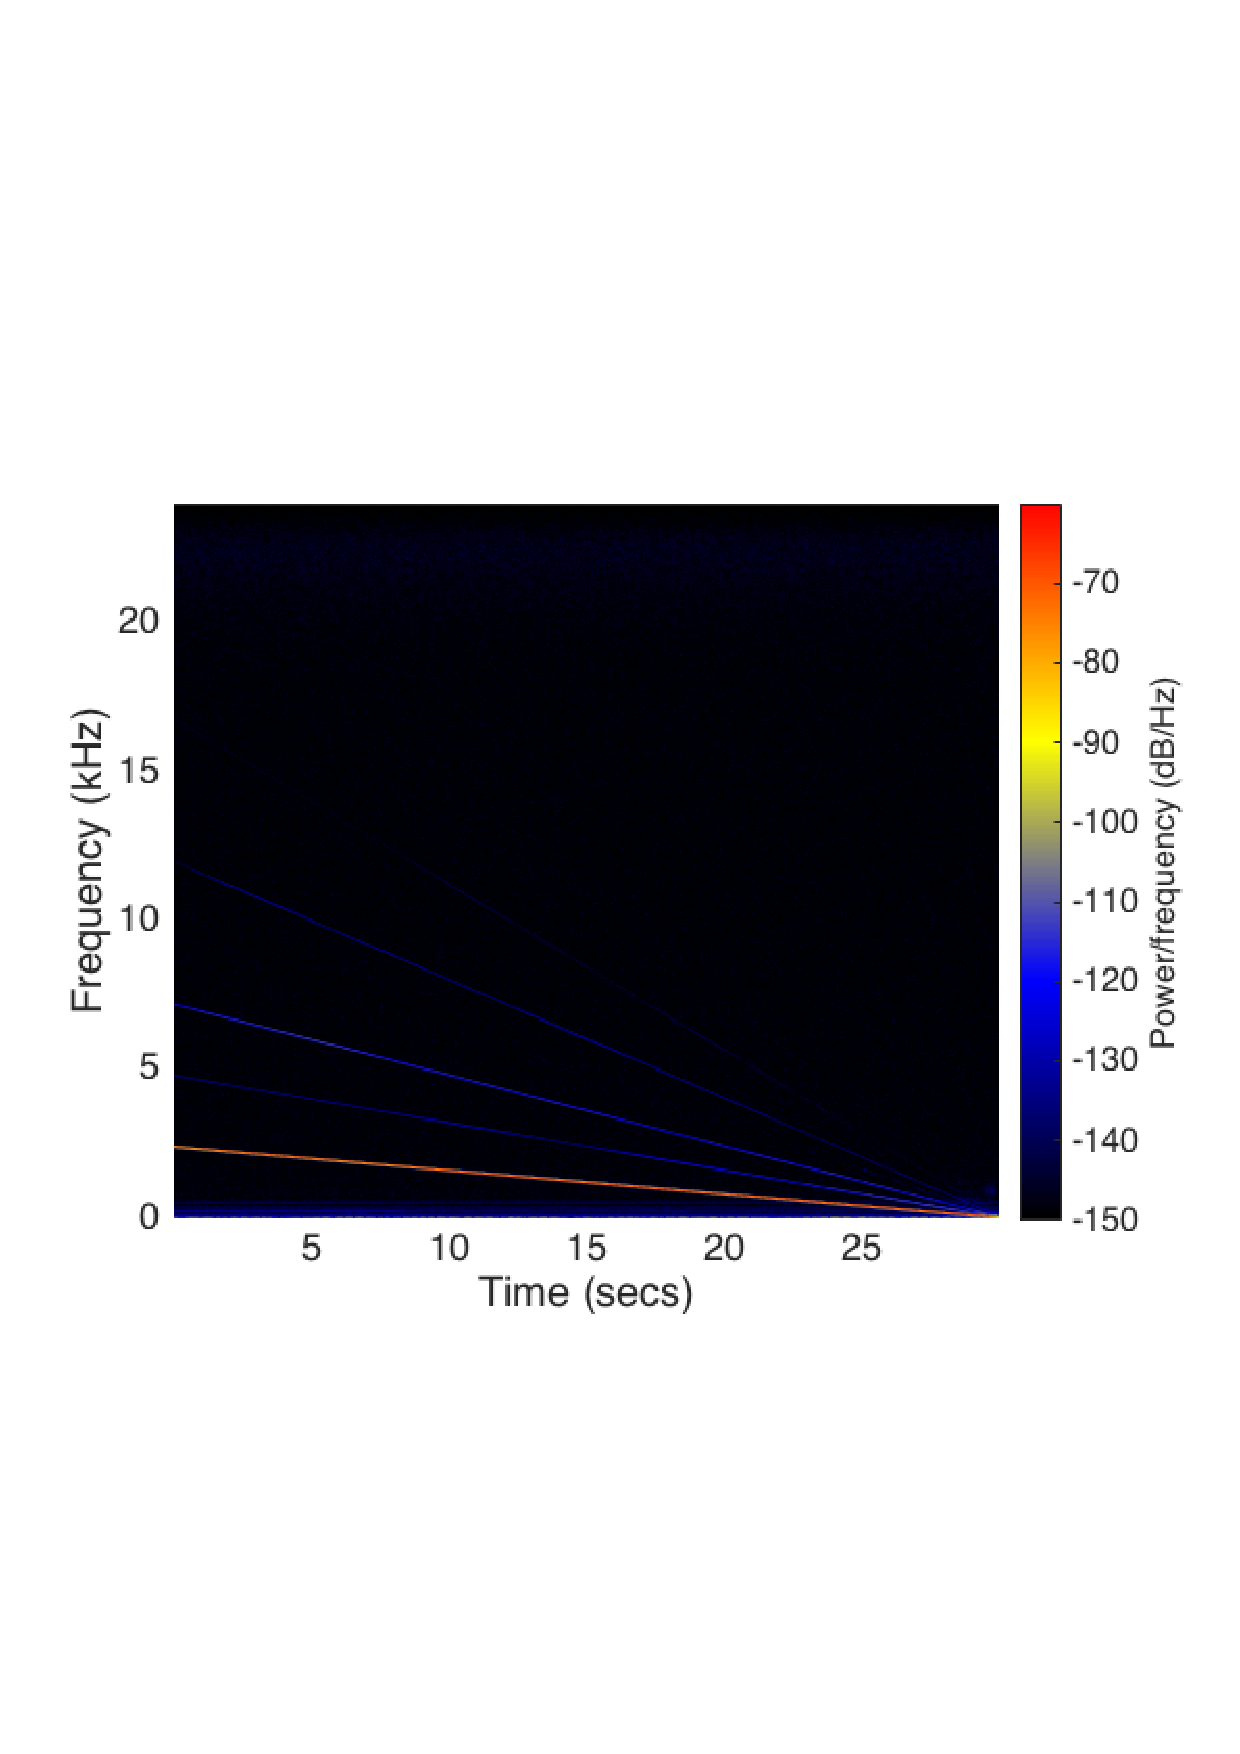
\includegraphics[width=1\textwidth]{figures/spectrogram_mic1.pdf}
	\caption{Microphone dataset 1.}
	\label{fig:spectrogram_mic1}
\end{subfigure}
\begin{subfigure}[t]{0.47\textwidth}
	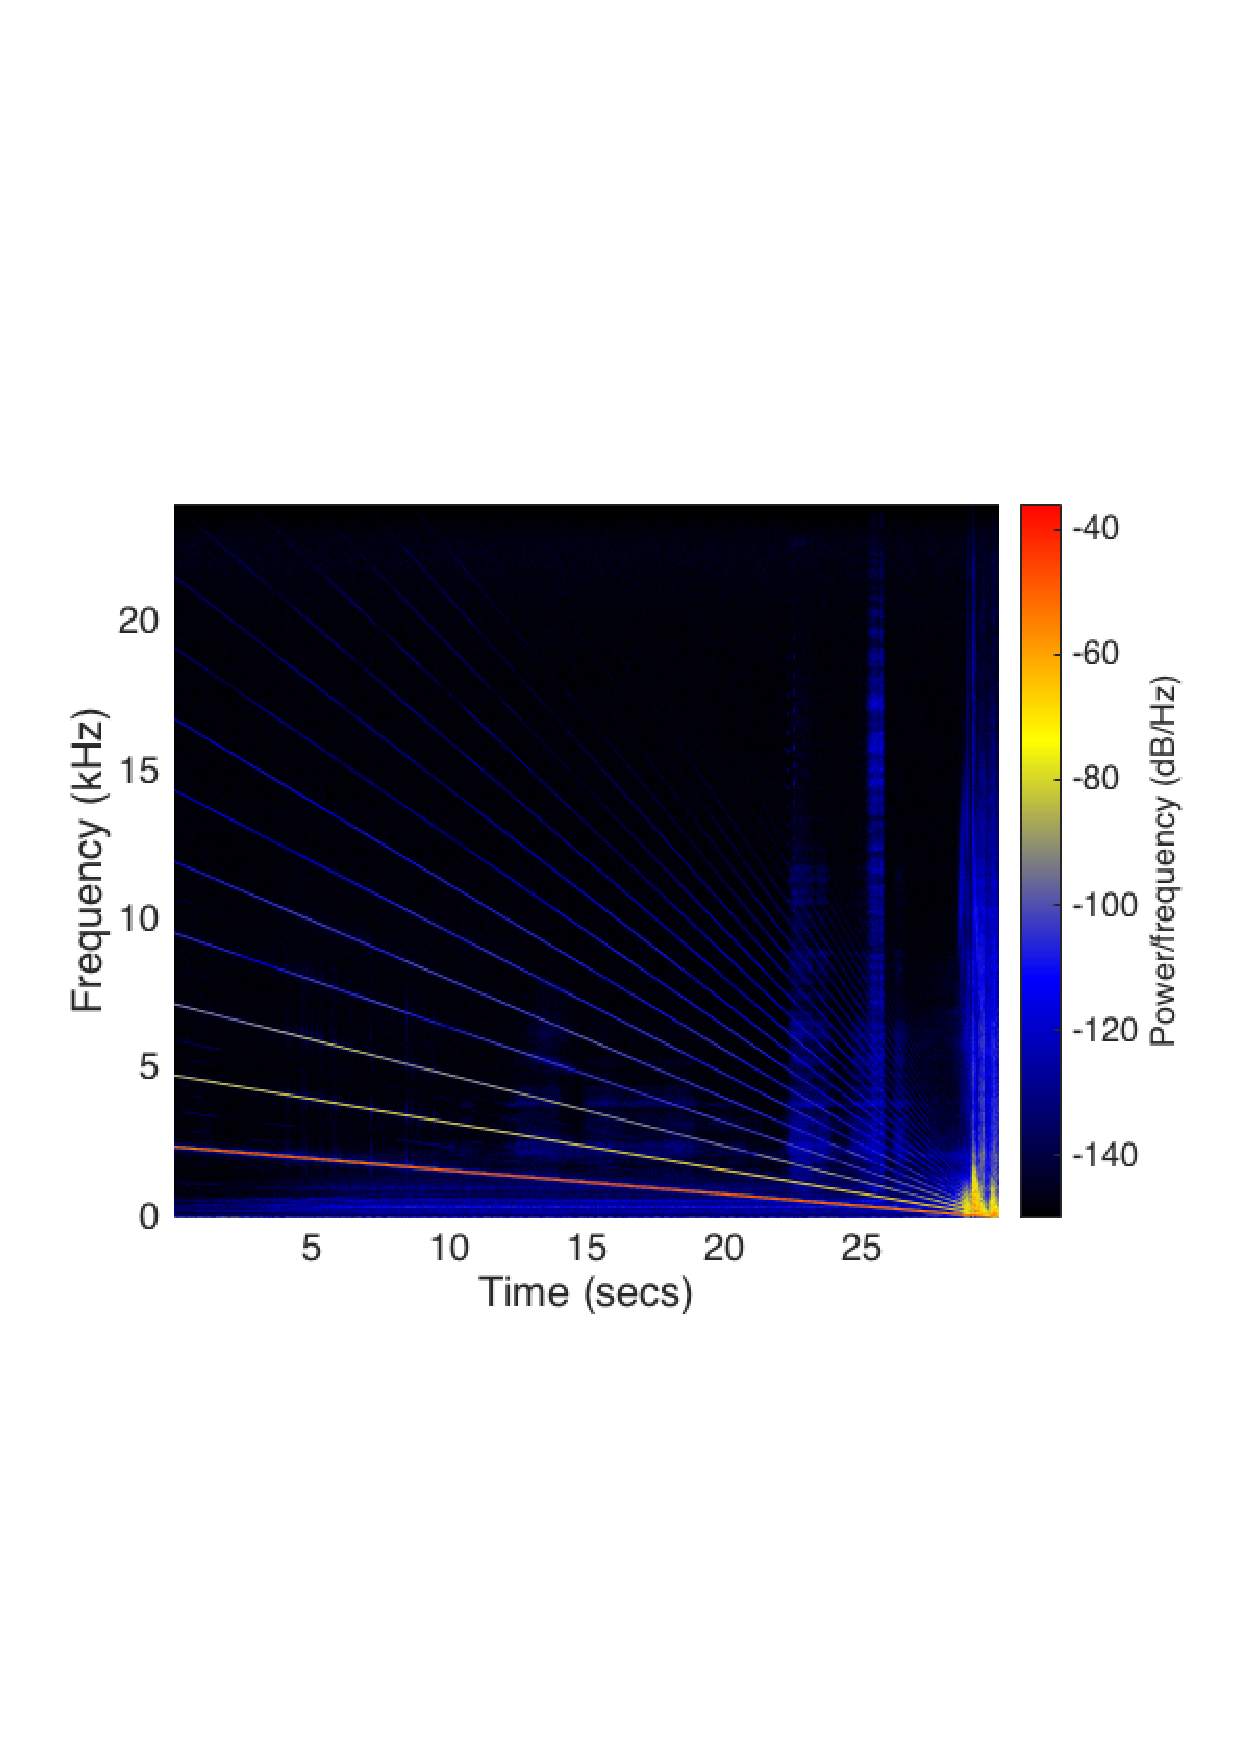
\includegraphics[width=1\textwidth]{figures/spectrogram_mic19.pdf}
	\caption{Microphone dataset 19.}
	\label{fig:spectrogram_mic19}
\end{subfigure}
\caption{The spectrograms of the microphone dataset 1 and 19. The prominent red line is the sine sweep from 2.4 kHz to 10 Hz while the yellow and blue lines along the red line are harmonic distortion.}
\label{fig:spec_mic}
\end{figure} 

The spectrograms of dataset 1 and 19, seen in \autoref{fig:spectrogram_mic1} and \autoref{fig:spectrogram_mic1}, show a prominent red line and three weak blue lines above the red line. It is seen that the red line is a linear decreasing function from 2.4 kHz to 10 Hz where the frequency is a function of time. This indicates that the red line is the fundamental frequency of the sine sweep from 2.4 kHz to 10 Hz. The blue and yellow line are linear functions of the harmonic distortions. The spectrograms clearly show that increasing the gain will increase the amount of harmonic distortion as well. An interesting observation is the spectral frequency leak that occurs at low frequency. 


\begin{figure}[H]
\centering
\begin{subfigure}[t]{0.47\textwidth}
	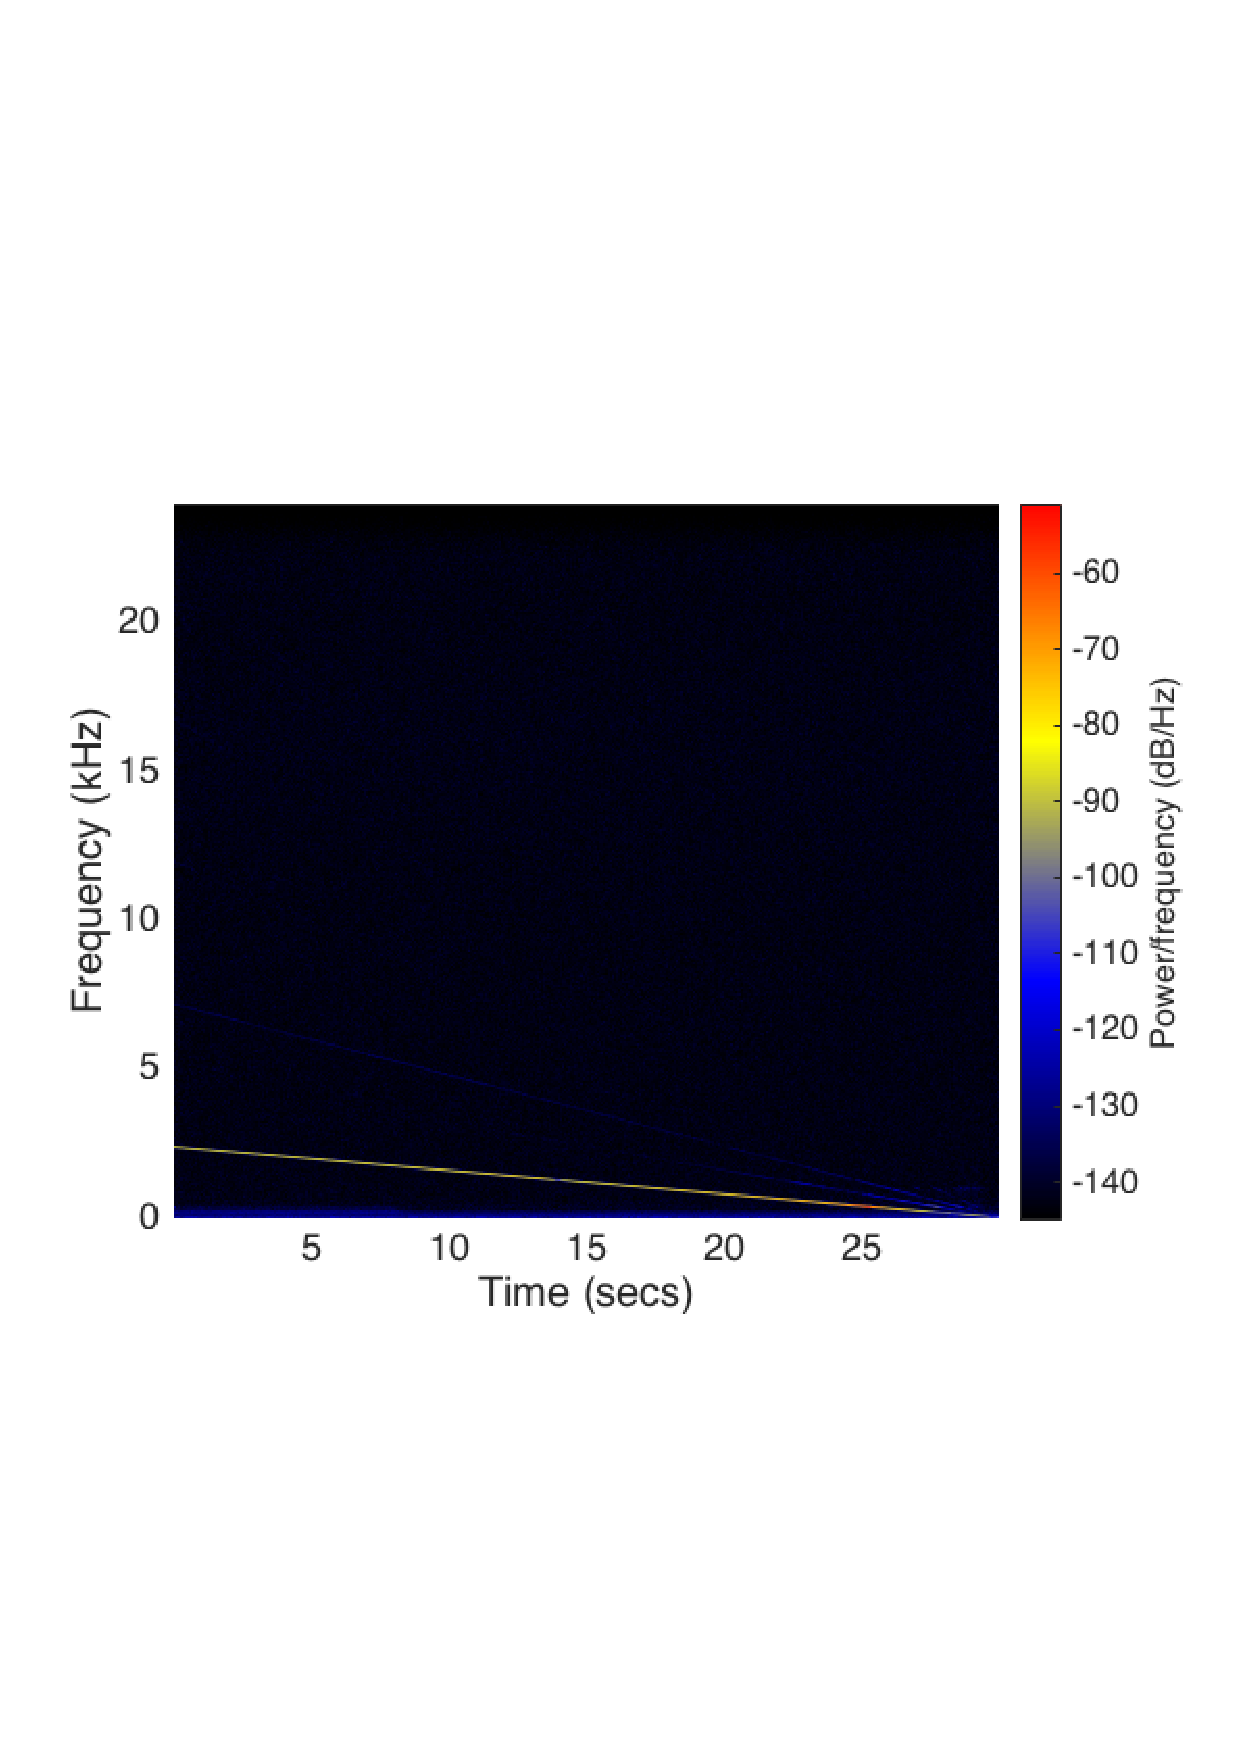
\includegraphics[width=1\textwidth]{figures/spectrogram_driver1.pdf}
	\caption{Vibration from driver.}
	\label{fig:spectrogram_driver1}
\end{subfigure}
\begin{subfigure}[t]{0.47\textwidth}
	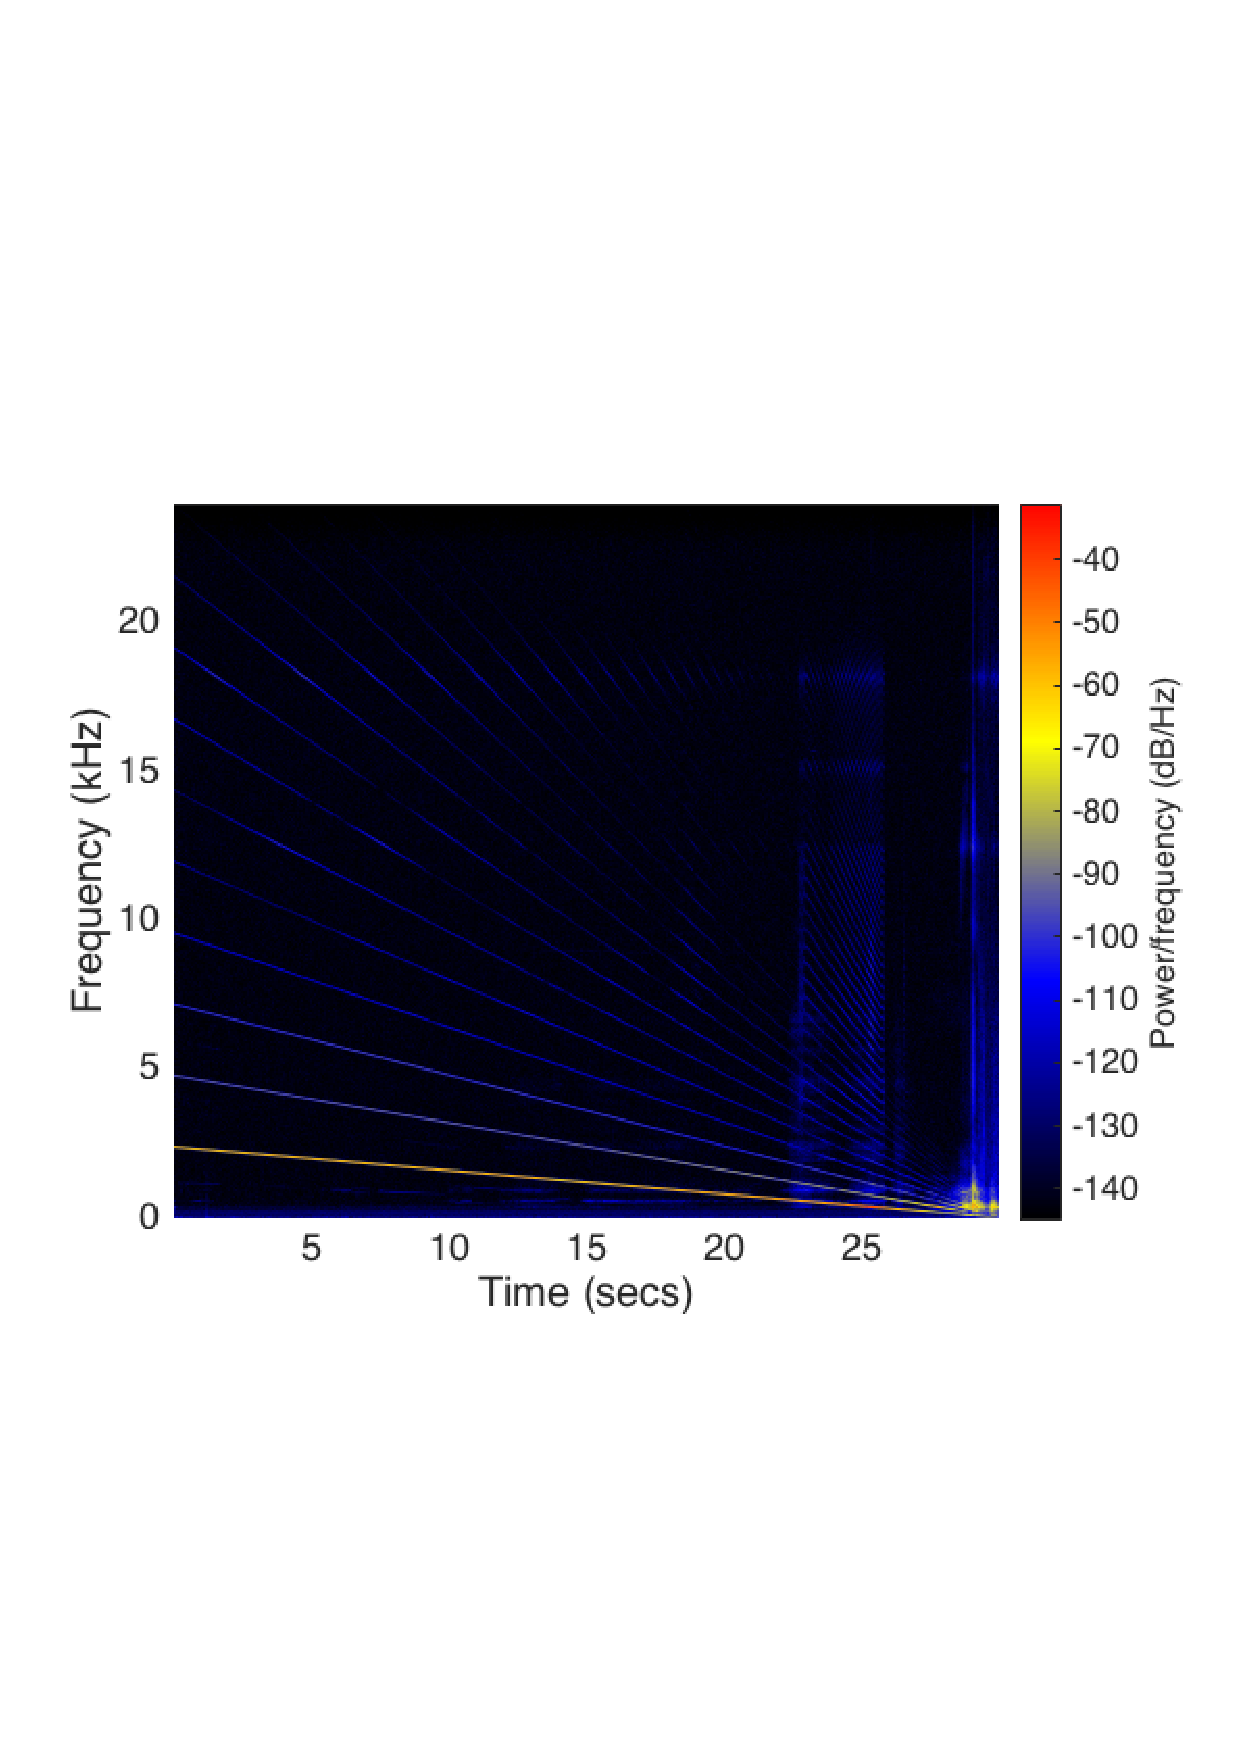
\includegraphics[width=1\textwidth]{figures/spectrogram_driver19.pdf}
	\caption{Vibration from driver.}
	\label{fig:spectrogram_driver19}
\end{subfigure}
\caption{The measured data of (a) the vibration on the driver, (b) the vibration on the enclosure, and (c) the sound pressure from the microphone. Dataset 20.}
\label{fig:spec_driver}
\end{figure} 























\subsubsection{Back Plate Hit Detection}\label{sec:hit_detect}
\todo[inline]{SKRIV NOGET MED 150W THRESHOLD}
As previously stated, it is possible that the loudspeaker coil hits the back plate of the driver if the coil moves too far back. In the long run this will damage the loudspeaker, and should therefore be avoided. In this section an analysis on how to detect these hits, will be provided. 

\textbf{From \autoref{subsec:impulses} the frequency response of a mechanical frame of a loudspeaker has the same characteristics as a low-pass filter. This means, if the coil is hitting the back plate of the driver, it will result in a increase in energy in the low frequency spectrum. As most music and loudspeakers have some sort of a high-pass filter implemented to remove almost non-audible sound, it can be assumed that only a back plate hit will generate vibrations at very low frequencies between, for instance, 0 Hz to 20 Hz. To examine if this is true, a section of the dataset 19 of the driver, where a hit is suspected to have occurred, is analysed.} %The analysed section is seen in \autoref{fig:raw_driver19_windows}.


%\begin{figure}[H]
%\centering
%\begin{subfigure}[t]{0.55\textwidth}
%	\tikzsetnextfilename{raw_driver19_window}
%	% This file was created by matlab2tikz.
%
%The latest updates can be retrieved from
%  http://www.mathworks.com/matlabcentral/fileexchange/22022-matlab2tikz-matlab2tikz
%where you can also make suggestions and rate matlab2tikz.
%
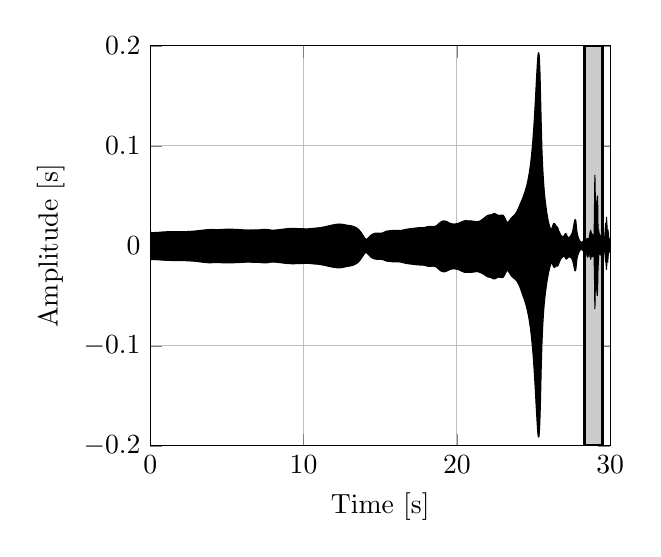
\begin{tikzpicture}

\begin{axis}[%
width=2.3in,
height=2in,
at={(1.011in,0.642in)},
scale only axis,
xmin=0,
xmax=30,
xmajorgrids,
ymin=-0.2,
ymax=0.2,
ymajorgrids,
xlabel={Time [s]},
ylabel={Amplitude [s]},
axis background/.style={fill=white}
]
\node[rectangle,draw, fill=black!20, minimum height=2in, minimum width=1pt, line width=1pt] at (axis cs:28.9,0) {};
\addplot[fill=black,draw=black,forget plot] plot table[row sep=crcr]{%
2.08333333333333e-05	0.0174441337585449\\
0.0250416666666667	0.013525128364563\\
0.0500625	0.013148307800293\\
0.0750833333333333	0.0131036043167114\\
0.100104166666667	0.0130690336227417\\
0.125125	0.0130878686904907\\
0.150145833333333	0.0131148099899292\\
0.175166666666667	0.0131456851959229\\
0.2001875	0.0131820440292358\\
0.225208333333333	0.0131937265396118\\
0.250229166666667	0.013242244720459\\
0.27525	0.0132321119308472\\
0.300270833333333	0.0132625102996826\\
0.325291666666667	0.0132992267608643\\
0.3503125	0.0133000612258911\\
0.375333333333333	0.0133060216903687\\
0.400354166666667	0.0133442878723145\\
0.425375	0.0133682489395142\\
0.450395833333333	0.0134040117263794\\
0.475416666666667	0.0134208202362061\\
0.5004375	0.0134366750717163\\
0.525458333333333	0.0134779214859009\\
0.550479166666667	0.013481616973877\\
0.5755	0.0135024785995483\\
0.600520833333333	0.0135313272476196\\
0.625541666666667	0.0135687589645386\\
0.6505625	0.0135985612869263\\
0.675583333333333	0.013633131980896\\
0.700604166666667	0.0136561393737793\\
0.725625	0.0136919021606445\\
0.750645833333333	0.0137306451797485\\
0.775666666666667	0.0137556791305542\\
0.8006875	0.01378333568573\\
0.825708333333333	0.0138041973114014\\
0.850729166666667	0.0138405561447144\\
0.87575	0.0138554573059082\\
0.900770833333333	0.0138554573059082\\
0.925791666666667	0.0138950347900391\\
0.9508125	0.0139113664627075\\
0.975833333333333	0.0139317512512207\\
1.00085416666667	0.0139557123184204\\
1.025875	0.0139747858047485\\
1.05089583333333	0.0140010118484497\\
1.07591666666667	0.0140320062637329\\
1.1009375	0.0140565633773804\\
1.12595833333333	0.0140770673751831\\
1.15097916666667	0.0140986442565918\\
1.176	0.0141662359237671\\
1.20102083333333	0.0141526460647583\\
1.22604166666667	0.0141149759292603\\
1.2510625	0.0141333341598511\\
1.27608333333333	0.0141546726226807\\
1.30110416666667	0.0141855478286743\\
1.326125	0.014235258102417\\
1.35114583333333	0.0142221450805664\\
1.37616666666667	0.0142310857772827\\
1.4011875	0.0142514705657959\\
1.42620833333333	0.0142489671707153\\
1.45122916666667	0.0142501592636108\\
1.47625	0.0142405033111572\\
1.50127083333333	0.0142426490783691\\
1.52629166666667	0.014230489730835\\
1.5513125	0.0142196416854858\\
1.57633333333333	0.0141897201538086\\
1.60135416666667	0.0141717195510864\\
1.626375	0.0141717195510864\\
1.65139583333333	0.0141562223434448\\
1.67641666666667	0.0141308307647705\\
1.7014375	0.0141433477401733\\
1.72645833333333	0.0141233205795288\\
1.75147916666667	0.0141158103942871\\
1.7765	0.0141146183013916\\
1.80152083333333	0.0140886306762695\\
1.82654166666667	0.0140882730484009\\
1.8515625	0.0140790939331055\\
1.87658333333333	0.0140920877456665\\
1.90160416666667	0.0140787363052368\\
1.926625	0.0140824317932129\\
1.95164583333333	0.014080286026001\\
1.97666666666667	0.0140800476074219\\
2.0016875	0.0140819549560547\\
2.02670833333333	0.0140724182128906\\
2.05172916666667	0.0140804052352905\\
2.07675	0.0140852928161621\\
2.10177083333333	0.0140907764434814\\
2.12679166666667	0.0141453742980957\\
2.1518125	0.0141433477401733\\
2.17683333333333	0.0141167640686035\\
2.20185416666667	0.014110803604126\\
2.226875	0.014117956161499\\
2.25189583333333	0.0141313076019287\\
2.27691666666667	0.01416015625\\
2.3019375	0.0141942501068115\\
2.32695833333333	0.0142010450363159\\
2.35197916666667	0.0142147541046143\\
2.377	0.0142277479171753\\
2.40202083333333	0.014255166053772\\
2.42704166666667	0.0142706632614136\\
2.4520625	0.0142948627471924\\
2.47708333333333	0.0143097639083862\\
2.50210416666667	0.014333963394165\\
2.527125	0.0143415927886963\\
2.55214583333333	0.0143803358078003\\
2.57716666666667	0.0144015550613403\\
2.6021875	0.0144282579421997\\
2.62720833333333	0.0144572257995605\\
2.65222916666667	0.0144776105880737\\
2.67725	0.0145164728164673\\
2.70227083333333	0.0145268440246582\\
2.72729166666667	0.0144838094711304\\
2.7523125	0.0145807266235352\\
2.77733333333333	0.0146057605743408\\
2.80235416666667	0.014631986618042\\
2.827375	0.0146661996841431\\
2.85239583333333	0.0147078037261963\\
2.87741666666667	0.0147354602813721\\
2.9024375	0.0147578716278076\\
2.92745833333333	0.0148038864135742\\
2.95247916666667	0.0148260593414307\\
2.9775	0.0148706436157227\\
3.00252083333333	0.0148930549621582\\
3.02754166666667	0.0149344205856323\\
3.0525625	0.0149737596511841\\
3.07758333333333	0.0150246620178223\\
3.10260416666667	0.0150657892227173\\
3.127625	0.0151075124740601\\
3.15264583333333	0.0151689052581787\\
3.17766666666667	0.0152368545532227\\
3.2026875	0.0152426958084106\\
3.22770833333333	0.0153077840805054\\
3.25272916666667	0.0153446197509766\\
3.27775	0.0153803825378418\\
3.30277083333333	0.0154129266738892\\
3.32779166666667	0.0154589414596558\\
3.3528125	0.0155411958694458\\
3.37783333333333	0.0155452489852905\\
3.40285416666667	0.0155919790267944\\
3.427875	0.0156158208847046\\
3.45289583333333	0.0156674385070801\\
3.47791666666667	0.0156955718994141\\
3.5029375	0.0157450437545776\\
3.52795833333333	0.0157967805862427\\
3.55297916666667	0.0158439874649048\\
3.578	0.0158843994140625\\
3.60302083333333	0.0159142017364502\\
3.62804166666667	0.0159745216369629\\
3.6530625	0.0160062313079834\\
3.67808333333333	0.0160480737686157\\
3.70310416666667	0.0160622596740723\\
3.728125	0.0160926580429077\\
3.75314583333333	0.0161361694335938\\
3.77816666666667	0.0161548852920532\\
3.8031875	0.0161689519882202\\
3.82820833333333	0.0162111520767212\\
3.85322916666667	0.0162196159362793\\
3.87825	0.0162382125854492\\
3.90327083333333	0.0162340402603149\\
3.92829166666667	0.0162550210952759\\
3.9533125	0.0162825584411621\\
3.97833333333333	0.016268253326416\\
4.00335416666667	0.0162605047225952\\
4.028375	0.0162662267684937\\
4.05339583333333	0.0162646770477295\\
4.07841666666667	0.0162562131881714\\
4.1034375	0.0162479877471924\\
4.12845833333333	0.0162286758422852\\
4.15347916666667	0.0162270069122314\\
4.1785	0.0162371397018433\\
4.20352083333333	0.0162290334701538\\
4.22854166666667	0.0162320137023926\\
4.2535625	0.0162011384963989\\
4.27858333333333	0.0161998271942139\\
4.30360416666667	0.0161756277084351\\
4.328625	0.0161881446838379\\
4.35364583333333	0.0161887407302856\\
4.37866666666667	0.0161789655685425\\
4.4036875	0.0161731243133545\\
4.42870833333333	0.0161886215209961\\
4.45372916666667	0.0162254571914673\\
4.47875	0.0162070989608765\\
4.50377083333333	0.0162215232849121\\
4.52879166666667	0.0162445306777954\\
4.5538125	0.0162478685379028\\
4.57883333333333	0.0162779092788696\\
4.60385416666667	0.0163146257400513\\
4.628875	0.0163321495056152\\
4.65389583333333	0.0163751840591431\\
4.67891666666667	0.0163940191268921\\
4.7039375	0.0164142847061157\\
4.72895833333333	0.0164343118667603\\
4.75397916666667	0.0164676904678345\\
4.779	0.0164873600006104\\
4.80402083333333	0.0164920091629028\\
4.82904166666667	0.0165045261383057\\
4.8540625	0.0165075063705444\\
4.87908333333333	0.0164927244186401\\
4.90410416666667	0.0165128707885742\\
4.929125	0.0165145397186279\\
4.95414583333333	0.0165392160415649\\
4.97916666666667	0.0165292024612427\\
5.0041875	0.0165307521820068\\
5.02920833333333	0.0165344476699829\\
5.05422916666667	0.0165383815765381\\
5.07925	0.0165324211120605\\
5.10427083333333	0.0165327787399292\\
5.12929166666667	0.0165436267852783\\
5.1543125	0.0165482759475708\\
5.17933333333333	0.0165408849716187\\
5.20435416666667	0.0165520906448364\\
5.229375	0.0165524482727051\\
5.25439583333333	0.0165770053863525\\
5.27941666666667	0.0165494680404663\\
5.3044375	0.0165427923202515\\
5.32945833333333	0.0165486335754395\\
5.35447916666667	0.016539454460144\\
5.3795	0.0165292024612427\\
5.40452083333333	0.0165024995803833\\
5.42954166666667	0.0165091753005981\\
5.4545625	0.0165070295333862\\
5.47958333333333	0.0164998769760132\\
5.50460416666667	0.0164941549301147\\
5.529625	0.0164831876754761\\
5.55464583333333	0.0164557695388794\\
5.57966666666667	0.0164422988891602\\
5.6046875	0.0164165496826172\\
5.62970833333333	0.0164107084274292\\
5.65472916666667	0.0163847208023071\\
5.67975	0.0163700580596924\\
5.70477083333333	0.0163614749908447\\
5.72979166666667	0.0163367986679077\\
5.7548125	0.0162984132766724\\
5.77983333333333	0.0162603855133057\\
5.80485416666667	0.0162379741668701\\
5.829875	0.0161999464035034\\
5.85489583333333	0.0161981582641602\\
5.87991666666667	0.0161627531051636\\
5.9049375	0.0161465406417847\\
5.92995833333333	0.016115665435791\\
5.95497916666667	0.0160897970199585\\
5.98	0.0160585641860962\\
6.00502083333333	0.0160255432128906\\
6.03004166666667	0.0159686803817749\\
6.0550625	0.0159963369369507\\
6.08008333333333	0.0159759521484375\\
6.10510416666667	0.0159282684326172\\
6.130125	0.015892505645752\\
6.15514583333333	0.0158891677856445\\
6.18016666666667	0.0158644914627075\\
6.2051875	0.0158466100692749\\
6.23020833333333	0.0158360004425049\\
6.25522916666667	0.0158376693725586\\
6.28025	0.0158051252365112\\
6.30527083333333	0.0157734155654907\\
6.33029166666667	0.0157642364501953\\
6.3553125	0.015750527381897\\
6.38033333333333	0.0157539844512939\\
6.40535416666667	0.0157500505447388\\
6.430375	0.0157680511474609\\
6.45539583333333	0.0157589912414551\\
6.48041666666667	0.0157626867294312\\
6.5054375	0.0157822370529175\\
6.53045833333333	0.0157740116119385\\
6.55547916666667	0.0157889127731323\\
6.5805	0.01578688621521\\
6.60552083333333	0.0157822370529175\\
6.63054166666667	0.015788197517395\\
6.6555625	0.0157915353775024\\
6.68058333333333	0.0158027410507202\\
6.70560416666667	0.0158090591430664\\
6.730625	0.0157994031906128\\
6.75564583333333	0.0158072710037231\\
6.78066666666667	0.0158181190490723\\
6.8056875	0.0157982110977173\\
6.83070833333333	0.0158140659332275\\
6.85572916666667	0.0158218145370483\\
6.88075	0.0158369541168213\\
6.90577083333333	0.015845775604248\\
6.93079166666667	0.0158636569976807\\
6.9558125	0.0158761739730835\\
6.98083333333333	0.0158882141113281\\
7.00585416666667	0.0158886909484863\\
7.030875	0.015921950340271\\
7.05589583333333	0.015964150428772\\
7.08091666666667	0.0159696340560913\\
7.1059375	0.0159767866134644\\
7.13095833333333	0.0160138607025146\\
7.15597916666667	0.0160485506057739\\
7.181	0.0161073207855225\\
7.20602083333333	0.0161236524581909\\
7.23104166666667	0.0161528587341309\\
7.2560625	0.0162006616592407\\
7.28108333333333	0.0162516832351685\\
7.30610416666667	0.0162925720214844\\
7.331125	0.0163209438323975\\
7.35614583333333	0.0163383483886719\\
7.38116666666667	0.0163733959197998\\
7.4061875	0.0163830518722534\\
7.43120833333333	0.0164109468460083\\
7.45622916666667	0.0164159536361694\\
7.48125	0.0164202451705933\\
7.50627083333333	0.01641845703125\\
7.53129166666667	0.0163898468017578\\
7.5563125	0.0163893699645996\\
7.58133333333333	0.0163614749908447\\
7.60635416666667	0.0163397789001465\\
7.631375	0.016291618347168\\
7.65639583333333	0.0162471532821655\\
7.68141666666667	0.0162198543548584\\
7.7064375	0.016148567199707\\
7.73145833333333	0.0160896778106689\\
7.75647916666667	0.016048789024353\\
7.7815	0.0159863233566284\\
7.80652083333333	0.0158941745758057\\
7.83154166666667	0.0158556699752808\\
7.8565625	0.0158106088638306\\
7.88158333333333	0.0157514810562134\\
7.90660416666667	0.0157146453857422\\
7.931625	0.0156705379486084\\
7.95664583333333	0.015657901763916\\
7.98166666666667	0.0156430006027222\\
8.0066875	0.015637993812561\\
8.03170833333333	0.0156441926956177\\
8.05672916666667	0.015630841255188\\
8.08175	0.0156583786010742\\
8.10677083333333	0.0156680345535278\\
8.13179166666667	0.0156958103179932\\
8.1568125	0.0157588720321655\\
8.18183333333333	0.0157665014266968\\
8.20685416666667	0.015811562538147\\
8.231875	0.0158299207687378\\
8.25689583333333	0.0158756971359253\\
8.28191666666667	0.0159240961074829\\
8.3069375	0.0159738063812256\\
8.33195833333333	0.0160108804702759\\
8.35697916666667	0.01605224609375\\
8.382	0.0161123275756836\\
8.40702083333333	0.0161582231521606\\
8.43204166666667	0.0161970853805542\\
8.4570625	0.0162638425827026\\
8.48208333333333	0.0163058042526245\\
8.50710416666667	0.0163264274597168\\
8.532125	0.0163748264312744\\
8.55714583333333	0.016425609588623\\
8.58216666666667	0.0164724588394165\\
8.6071875	0.0164806842803955\\
8.63220833333333	0.0165771245956421\\
8.65722916666667	0.0166155099868774\\
8.68225	0.0166538953781128\\
8.70727083333333	0.0166980028152466\\
8.73229166666667	0.0167548656463623\\
8.7573125	0.0168157815933228\\
8.78233333333333	0.0168620347976685\\
8.80735416666667	0.0168946981430054\\
8.832375	0.0169271230697632\\
8.85739583333333	0.0169821977615356\\
8.88241666666667	0.0170294046401978\\
8.9074375	0.0170701742172241\\
8.93245833333333	0.0171375274658203\\
8.95747916666667	0.0171374082565308\\
8.9825	0.0171587467193604\\
9.00752083333333	0.0172109603881836\\
9.03254166666667	0.017237663269043\\
9.0575625	0.0172935724258423\\
9.08258333333333	0.0173063278198242\\
9.10760416666667	0.0173218250274658\\
9.132625	0.0173497200012207\\
9.15764583333333	0.0173478126525879\\
9.18266666666667	0.0173822641372681\\
9.2076875	0.0173777341842651\\
9.23270833333333	0.0174020528793335\\
9.25772916666667	0.0174028873443604\\
9.28275	0.0174024105072021\\
9.30777083333333	0.0174020528793335\\
9.33279166666667	0.017372727394104\\
9.3578125	0.017397403717041\\
9.38283333333333	0.017382025718689\\
9.40785416666667	0.0173285007476807\\
9.432875	0.017330527305603\\
9.45789583333333	0.0173323154449463\\
9.48291666666667	0.0173298120498657\\
9.5079375	0.0173071622848511\\
9.53295833333333	0.0172946453094482\\
9.55797916666667	0.0172981023788452\\
9.583	0.0172525644302368\\
9.60802083333333	0.0172533988952637\\
9.63304166666667	0.0172268152236938\\
9.6580625	0.0172150135040283\\
9.68308333333333	0.0172126293182373\\
9.70810416666667	0.0172011852264404\\
9.733125	0.0171859264373779\\
9.75814583333333	0.0171804428100586\\
9.78316666666667	0.0171525478363037\\
9.8081875	0.0171377658843994\\
9.83320833333334	0.0171386003494263\\
9.85822916666667	0.0171124935150146\\
9.88325	0.0171166658401489\\
9.90827083333333	0.0170993804931641\\
9.93329166666667	0.0170944929122925\\
9.9583125	0.0170706510543823\\
9.98333333333333	0.0170501470565796\\
10.0083541666667	0.0170356035232544\\
10.033375	0.0169914960861206\\
10.0583958333333	0.0170005559921265\\
10.0834166666667	0.0170102119445801\\
10.1084375	0.0169705152511597\\
10.1334583333333	0.0169491767883301\\
10.1584791666667	0.0169483423233032\\
10.1835	0.0169246196746826\\
10.2085208333333	0.0169349908828735\\
10.2335416666667	0.016913890838623\\
10.2585625	0.016938328742981\\
10.2835833333333	0.0169572830200195\\
10.3086041666667	0.0169775485992432\\
10.333625	0.016999363899231\\
10.3586458333333	0.0170327425003052\\
10.3836666666667	0.0170744657516479\\
10.4086875	0.0170915126800537\\
10.4337083333333	0.0171260833740234\\
10.4587291666667	0.0171712636947632\\
10.48375	0.0172317028045654\\
10.5087708333333	0.0172442197799683\\
10.5337916666667	0.0172771215438843\\
10.5588125	0.017345666885376\\
10.5838333333333	0.0173889398574829\\
10.6088541666667	0.0174278020858765\\
10.633875	0.0174736976623535\\
10.6588958333333	0.0175179243087769\\
10.6839166666667	0.017504096031189\\
10.7089375	0.0175975561141968\\
10.7339583333333	0.0176342725753784\\
10.7589791666667	0.0176651477813721\\
10.784	0.0177170038223267\\
10.8090208333333	0.0177382230758667\\
10.8340416666667	0.0177578926086426\\
10.8590625	0.0177834033966064\\
10.8840833333333	0.0178287029266357\\
10.9091041666667	0.0178596973419189\\
10.934125	0.0178934335708618\\
10.9591458333333	0.0179351568222046\\
10.9841666666667	0.0179930925369263\\
11.0091875	0.0180190801620483\\
11.0342083333333	0.0180590152740479\\
11.0592291666667	0.0180873870849609\\
11.08425	0.0181617736816406\\
11.1092708333333	0.0181983709335327\\
11.1342916666667	0.0182547569274902\\
11.1593125	0.018323540687561\\
11.1843333333333	0.018383264541626\\
11.2093541666667	0.0184645652770996\\
11.234375	0.0185511112213135\\
11.2593958333333	0.0186281204223633\\
11.2844166666667	0.0186648368835449\\
11.3094375	0.0187809467315674\\
11.3344583333333	0.0188539028167725\\
11.3594791666667	0.0189625024795532\\
11.3845	0.0190408229827881\\
11.4095208333333	0.0191167593002319\\
11.4345416666667	0.0191928148269653\\
11.4595625	0.019289493560791\\
11.4845833333333	0.0194246768951416\\
11.5096041666667	0.0194790363311768\\
11.534625	0.0195668935775757\\
11.5596458333333	0.0196346044540405\\
11.5846666666667	0.0197362899780273\\
11.6096875	0.0198198556900024\\
11.6347083333333	0.0198944807052612\\
11.6597291666667	0.0199992656707764\\
11.68475	0.0200852155685425\\
11.7097708333333	0.0201708078384399\\
11.7347916666667	0.0202442407608032\\
11.7598125	0.0203417539596558\\
11.7848333333333	0.020447850227356\\
11.8098541666667	0.0205179452896118\\
11.834875	0.020601749420166\\
11.8598958333333	0.0206559896469116\\
11.8849166666667	0.0207802057266235\\
11.9099375	0.0208553075790405\\
11.9349583333333	0.0209276676177979\\
11.9599791666667	0.0209884643554688\\
11.985	0.0210902690887451\\
12.0100208333333	0.0211566686630249\\
12.0350416666667	0.0212430953979492\\
12.0600625	0.0213093757629395\\
12.0850833333333	0.0213801860809326\\
12.1101041666667	0.0214052200317383\\
12.135125	0.0214844942092896\\
12.1601458333333	0.0215476751327515\\
12.1851666666667	0.0216346979141235\\
12.2101875	0.0216710567474365\\
12.2352083333333	0.0217214822769165\\
12.2602291666667	0.0217512845993042\\
12.28525	0.0217370986938477\\
12.3102708333333	0.0217386484146118\\
12.3352916666667	0.0217440128326416\\
12.3603125	0.0217629671096802\\
12.3853333333333	0.0217190980911255\\
12.4103541666667	0.0217164754867554\\
12.435375	0.0216363668441772\\
12.4603958333333	0.0216211080551147\\
12.4854166666667	0.021581768989563\\
12.5104375	0.0215216875076294\\
12.5354583333333	0.021467924118042\\
12.5604791666667	0.0213643312454224\\
12.5855	0.021304726600647\\
12.6105208333333	0.0212384462356567\\
12.6355416666667	0.0211762189865112\\
12.6605625	0.0210961103439331\\
12.6855833333333	0.0210355520248413\\
12.7106041666667	0.0209527015686035\\
12.735625	0.0208666324615479\\
12.7606458333333	0.0208185911178589\\
12.7856666666667	0.0207582712173462\\
12.8106875	0.0206890106201172\\
12.8357083333333	0.0206308364868164\\
12.8607291666667	0.0205554962158203\\
12.88575	0.0205261707305908\\
12.9107708333333	0.0204222202301025\\
12.9357916666667	0.0204188823699951\\
12.9608125	0.0203204154968262\\
12.9858333333333	0.0202691555023193\\
13.0108541666667	0.0202019214630127\\
13.035875	0.0201456546783447\\
13.0608958333333	0.0200655460357666\\
13.0859166666667	0.0200191736221313\\
13.1109375	0.0199253559112549\\
13.1359583333333	0.0198445320129395\\
13.1609791666667	0.0197505950927734\\
13.186	0.0197038650512695\\
13.2110208333333	0.0195786952972412\\
13.2360416666667	0.019476056098938\\
13.2610625	0.0193073749542236\\
13.2860833333333	0.0191764831542969\\
13.3111041666667	0.0190207958221436\\
13.336125	0.0188961029052734\\
13.3611458333333	0.0186749696731567\\
13.3861666666667	0.0185122489929199\\
13.4111875	0.0183169841766357\\
13.4362083333333	0.0180661678314209\\
13.4612291666667	0.017853856086731\\
13.48625	0.0175918340682983\\
13.5112708333333	0.0173110961914062\\
13.5362916666667	0.0169925689697266\\
13.5613125	0.0166597366333008\\
13.5863333333333	0.0163099765777588\\
13.6113541666667	0.0159174203872681\\
13.636375	0.0155293941497803\\
13.6613958333333	0.0150763988494873\\
13.6864166666667	0.0146143436431885\\
13.7114375	0.014168381690979\\
13.7364583333333	0.0136096477508545\\
13.7614791666667	0.0130655765533447\\
13.7865	0.0125436782836914\\
13.8115208333333	0.0119357109069824\\
13.8365416666667	0.0113338232040405\\
13.8615625	0.0106756687164307\\
13.8865833333333	0.0100915431976318\\
13.9116041666667	0.00947129726409912\\
13.936625	0.00886750221252441\\
13.9616458333333	0.00825822353363037\\
13.9866666666667	0.00778257846832275\\
14.0116875	0.00735759735107422\\
14.0367083333333	0.00696361064910889\\
14.0617291666667	0.00667524337768555\\
14.08675	0.00652050971984863\\
14.1117708333333	0.00652647018432617\\
14.1367916666667	0.00670945644378662\\
14.1618125	0.00699913501739502\\
14.1868333333333	0.00733792781829834\\
14.2118541666667	0.0077139139175415\\
14.236875	0.00815272331237793\\
14.2618958333333	0.00860869884490967\\
14.2869166666667	0.00900518894195557\\
14.3119375	0.00939702987670898\\
14.3369583333333	0.00978922843933105\\
14.3619791666667	0.0101321935653687\\
14.387	0.0104804039001465\\
14.4120208333333	0.0107772350311279\\
14.4370416666667	0.0110471248626709\\
14.4620625	0.0112928152084351\\
14.4870833333333	0.0115351676940918\\
14.5121041666667	0.0117450952529907\\
14.537125	0.0118981599807739\\
14.5621458333333	0.0120600461959839\\
14.5871666666667	0.0121918916702271\\
14.6121875	0.0123043060302734\\
14.6372083333333	0.0123888254165649\\
14.6622291666667	0.0124760866165161\\
14.68725	0.0125365257263184\\
14.7122708333333	0.0126163959503174\\
14.7372916666667	0.0126279592514038\\
14.7623125	0.0126475095748901\\
14.7873333333333	0.0126579999923706\\
14.8123541666667	0.0126771926879883\\
14.837375	0.0126643180847168\\
14.8623958333333	0.0126522779464722\\
14.8874166666667	0.0126442909240723\\
14.9124375	0.0126438140869141\\
14.9374583333333	0.0126296281814575\\
14.9624791666667	0.0126005411148071\\
14.9875	0.0125808715820312\\
15.0125208333333	0.0125870704650879\\
15.0375416666667	0.0125871896743774\\
15.0625625	0.0126022100448608\\
15.0875833333333	0.0126547813415527\\
15.1126041666667	0.0127360820770264\\
15.137625	0.0128141641616821\\
15.1626458333333	0.0129730701446533\\
15.1876666666667	0.0131022930145264\\
15.2126875	0.0132739543914795\\
15.2377083333333	0.0134528875350952\\
15.2627291666667	0.0136306285858154\\
15.28775	0.0138425827026367\\
15.3127708333333	0.0140299797058105\\
15.3377916666667	0.014187216758728\\
15.3628125	0.0143324136734009\\
15.3878333333333	0.0144814252853394\\
15.4128541666667	0.0145851373672485\\
15.437875	0.0147069692611694\\
15.4628958333333	0.0147304534912109\\
15.4879166666667	0.014826774597168\\
15.5129375	0.0148801803588867\\
15.5379583333333	0.0149414539337158\\
15.5629791666667	0.0149836540222168\\
15.588	0.0150250196456909\\
15.6130208333333	0.0150867700576782\\
15.6380416666667	0.0151267051696777\\
15.6630625	0.0151498317718506\\
15.6880833333333	0.0151907205581665\\
15.7131041666667	0.0152368545532227\\
15.738125	0.0152875185012817\\
15.7631458333333	0.0153127908706665\\
15.7881666666667	0.015317440032959\\
15.8131875	0.0153570175170898\\
15.8382083333333	0.0153809785842896\\
15.8632291666667	0.0153845548629761\\
15.88825	0.0154021978378296\\
15.9132708333333	0.0154201984405518\\
15.9382916666667	0.0154287815093994\\
15.9633125	0.0154200792312622\\
15.9883333333333	0.0154142379760742\\
16.0133541666667	0.0154227018356323\\
16.038375	0.0153951644897461\\
16.0633958333333	0.0153549909591675\\
16.0884166666667	0.0153504610061646\\
16.1134375	0.015299916267395\\
16.1384583333333	0.0152820348739624\\
16.1634791666667	0.0152640342712402\\
16.1885	0.0152740478515625\\
16.2135208333333	0.0152524709701538\\
16.2385416666667	0.0152736902236938\\
16.2635625	0.0152624845504761\\
16.2885833333333	0.0152912139892578\\
16.3136041666667	0.0153496265411377\\
16.338625	0.015373706817627\\
16.3636458333333	0.0154263973236084\\
16.3886666666667	0.0154972076416016\\
16.4136875	0.0155841112136841\\
16.4387083333333	0.0156378746032715\\
16.4637291666667	0.01569664478302\\
16.48875	0.015790581703186\\
16.5137708333333	0.0158723592758179\\
16.5387916666667	0.0159751176834106\\
16.5638125	0.0160551071166992\\
16.5888333333333	0.0161577463150024\\
16.6138541666667	0.0162507295608521\\
16.638875	0.0163224935531616\\
16.6638958333333	0.0163685083389282\\
16.6889166666667	0.0164364576339722\\
16.7139375	0.0165036916732788\\
16.7389583333333	0.0165603160858154\\
16.7639791666667	0.0166410207748413\\
16.789	0.0167248249053955\\
16.8140208333333	0.0167744159698486\\
16.8390416666667	0.016828179359436\\
16.8640625	0.0168788433074951\\
16.8890833333333	0.0169576406478882\\
16.9141041666667	0.016994833946228\\
16.939125	0.0170410871505737\\
16.9641458333333	0.0170806646347046\\
16.9891666666667	0.017139196395874\\
17.0141875	0.0172109603881836\\
17.0392083333333	0.0172618627548218\\
17.0642291666667	0.0173348188400269\\
17.08925	0.0173755884170532\\
17.1142708333333	0.0174448490142822\\
17.1392916666667	0.0174486637115479\\
17.1643125	0.0174803733825684\\
17.1893333333333	0.017526388168335\\
17.2143541666667	0.0175930261611938\\
17.239375	0.0176322460174561\\
17.2643958333333	0.0176610946655273\\
17.2894166666667	0.0177028179168701\\
17.3144375	0.0177712440490723\\
17.3394583333333	0.017817497253418\\
17.3644791666667	0.0178496837615967\\
17.3895	0.0178635120391846\\
17.4145208333333	0.0179288387298584\\
17.4395416666667	0.017961859703064\\
17.4645625	0.017999529838562\\
17.4895833333333	0.018022894859314\\
17.5146041666667	0.018062949180603\\
17.539625	0.0180728435516357\\
17.5646458333333	0.01810622215271\\
17.5896666666667	0.0180763006210327\\
17.6146875	0.0180631875991821\\
17.6397083333333	0.0180815458297729\\
17.6647291666667	0.0180732011795044\\
17.68975	0.0180611610412598\\
17.7147708333333	0.0180732011795044\\
17.7397916666667	0.0180991888046265\\
17.7648125	0.018126368522644\\
17.7898333333333	0.0181397199630737\\
17.8148541666667	0.0181893110275269\\
17.839875	0.0182832479476929\\
17.8648958333333	0.0183231830596924\\
17.8899166666667	0.0183992385864258\\
17.9149375	0.0184700489044189\\
17.9399583333333	0.0185521841049194\\
17.9649791666667	0.0186257362365723\\
17.99	0.0187492370605469\\
18.0150208333333	0.0188664197921753\\
18.0400416666667	0.0189815759658813\\
18.0650625	0.0190328359603882\\
18.0900833333333	0.0191329717636108\\
18.1151041666667	0.0192264318466187\\
18.140125	0.0192656517028809\\
18.1651458333333	0.0192974805831909\\
18.1901666666667	0.0193121433258057\\
18.2151875	0.0193363428115845\\
18.2402083333333	0.0193533897399902\\
18.2652291666667	0.0193248987197876\\
18.29025	0.0193346738815308\\
18.3152708333333	0.0193099975585938\\
18.3402916666667	0.0192739963531494\\
18.3653125	0.0192720890045166\\
18.3903333333333	0.0192562341690063\\
18.4153541666667	0.0192611217498779\\
18.440375	0.0192636251449585\\
18.4653958333333	0.0192465782165527\\
18.4904166666667	0.0192739963531494\\
18.5154375	0.0192666053771973\\
18.5404583333333	0.0192996263504028\\
18.5654791666667	0.0193842649459839\\
18.5905	0.0194982290267944\\
18.6155208333333	0.0196996927261353\\
18.6405416666667	0.0198712348937988\\
18.6655625	0.0201015472412109\\
18.6905833333333	0.02039635181427\\
18.7156041666667	0.0207115411758423\\
18.740625	0.02104651927948\\
18.7656458333333	0.0213632583618164\\
18.7906666666667	0.0217374563217163\\
18.8156875	0.0221004486083984\\
18.8407083333333	0.0224542617797852\\
18.8657291666667	0.0227910280227661\\
18.89075	0.023115873336792\\
18.9157708333333	0.0234055519104004\\
18.9407916666667	0.0236350297927856\\
18.9658125	0.0238840579986572\\
18.9908333333333	0.0240856409072876\\
19.0158541666667	0.0243097543716431\\
19.040875	0.0244883298873901\\
19.0658958333333	0.0246367454528809\\
19.0909166666667	0.0247553586959839\\
19.1159375	0.0248157978057861\\
19.1409583333333	0.0248211622238159\\
19.1659791666667	0.0248291492462158\\
19.191	0.0247656106948853\\
19.2160208333333	0.0247126817703247\\
19.2410416666667	0.0246188640594482\\
19.2660625	0.0245308876037598\\
19.2910833333333	0.024416446685791\\
19.3161041666667	0.0243091583251953\\
19.341125	0.0241603851318359\\
19.3661458333333	0.0239905118942261\\
19.3911666666667	0.0237839221954346\\
19.4161875	0.0236095190048218\\
19.4412083333333	0.0234092473983765\\
19.4662291666667	0.0231764316558838\\
19.49125	0.0229754447937012\\
19.5162708333333	0.022815465927124\\
19.5412916666667	0.0226483345031738\\
19.5663125	0.0224692821502686\\
19.5913333333333	0.0223290920257568\\
19.6163541666667	0.0222113132476807\\
19.641375	0.0221070051193237\\
19.6663958333333	0.0220341682434082\\
19.6914166666667	0.0219175815582275\\
19.7164375	0.0218663215637207\\
19.7414583333333	0.0218421220779419\\
19.7664791666667	0.0217581987380981\\
19.7915	0.021744966506958\\
19.8165208333333	0.0217596292495728\\
19.8415416666667	0.0217770338058472\\
19.8665625	0.0217828750610352\\
19.8915833333333	0.0218362808227539\\
19.9166041666667	0.0218791961669922\\
19.941625	0.0219467878341675\\
19.9666458333333	0.0220240354537964\\
19.9916666666667	0.0220874547958374\\
20.0166875	0.0221959352493286\\
20.0417083333333	0.022313117980957\\
20.0667291666667	0.0224117040634155\\
20.09175	0.0225427150726318\\
20.1167708333333	0.0226690769195557\\
20.1417916666667	0.0228263139724731\\
20.1668125	0.0229573249816895\\
20.1918333333333	0.0231013298034668\\
20.2168541666667	0.0232757329940796\\
20.241875	0.0234352350234985\\
20.2668958333333	0.0236291885375977\\
20.2919166666667	0.0237768888473511\\
20.3169375	0.023958683013916\\
20.3419583333333	0.0241364240646362\\
20.3669791666667	0.0242964029312134\\
20.392	0.0244518518447876\\
20.4170208333333	0.0246180295944214\\
20.4420416666667	0.0247514247894287\\
20.4670625	0.0248813629150391\\
20.4920833333333	0.0249801874160767\\
20.5171041666667	0.0250335931777954\\
20.542125	0.0250766277313232\\
20.5671458333333	0.0250948667526245\\
20.5921666666667	0.0251015424728394\\
20.6171875	0.0250868797302246\\
20.6422083333333	0.025084376335144\\
20.6672291666667	0.0250357389450073\\
20.69225	0.0249865055084229\\
20.7172708333333	0.0249638557434082\\
20.7422916666667	0.0249263048171997\\
20.7673125	0.0249083042144775\\
20.7923333333333	0.0248900651931763\\
20.8173541666667	0.0248545408248901\\
20.842375	0.0248538255691528\\
20.8673958333333	0.0248371362686157\\
20.8924166666667	0.0248321294784546\\
20.9174375	0.0248321294784546\\
20.9424583333333	0.0248123407363892\\
20.9674791666667	0.0248016119003296\\
20.9925	0.0247378349304199\\
21.0175208333333	0.0246872901916504\\
21.0425416666667	0.0246568918228149\\
21.0675625	0.0245620012283325\\
21.0925833333333	0.0245187282562256\\
21.1176041666667	0.0244406461715698\\
21.142625	0.0243560075759888\\
21.1676458333333	0.0242875814437866\\
21.1926666666667	0.0241986513137817\\
21.2176875	0.0241419076919556\\
21.2427083333333	0.0241051912307739\\
21.2677291666667	0.0240743160247803\\
21.29275	0.0240596532821655\\
21.3177708333333	0.0240672826766968\\
21.3427916666667	0.0241365432739258\\
21.3678125	0.0242211818695068\\
21.3928333333333	0.0242770910263062\\
21.4178541666667	0.0243664979934692\\
21.442875	0.0245187282562256\\
21.4678958333333	0.0246692895889282\\
21.4929166666667	0.0248323678970337\\
21.5179375	0.0250157117843628\\
21.5429583333333	0.0251970291137695\\
21.5679791666667	0.0254095792770386\\
21.593	0.0256576538085938\\
21.6180208333333	0.0259164571762085\\
21.6430416666667	0.0261667966842651\\
21.6680625	0.0264409780502319\\
21.6930833333333	0.0267170667648315\\
21.7181041666667	0.0269858837127686\\
21.743125	0.0273033380508423\\
21.7681458333333	0.0276157855987549\\
21.7931666666667	0.0278679132461548\\
21.8181875	0.0282278060913086\\
21.8432083333333	0.0285413265228271\\
21.8682291666667	0.0288461446762085\\
21.89325	0.029139518737793\\
21.9182708333333	0.0294617414474487\\
21.9432916666667	0.0297086238861084\\
21.9683125	0.0300043821334839\\
21.9933333333333	0.0302213430404663\\
22.0183541666667	0.0304399728775024\\
22.043375	0.0305919647216797\\
22.0683958333333	0.0306967496871948\\
22.0934166666667	0.0307843685150146\\
22.1184375	0.0307987928390503\\
22.1434583333333	0.030825138092041\\
22.1684791666667	0.0308159589767456\\
22.1935	0.0308229923248291\\
22.2185208333333	0.0309444665908813\\
22.2435416666667	0.0311071872711182\\
22.2685625	0.0312448740005493\\
22.2935833333333	0.0314546823501587\\
22.3186041666667	0.0316667556762695\\
22.343625	0.0318219661712646\\
22.3686458333333	0.0320000648498535\\
22.3936666666667	0.0320919752120972\\
22.4186875	0.0321664810180664\\
22.4437083333333	0.0321915149688721\\
22.4687291666667	0.0321606397628784\\
22.49375	0.0321078300476074\\
22.5187708333333	0.031922459602356\\
22.5437916666667	0.0317248106002808\\
22.5688125	0.031496524810791\\
22.5938333333333	0.0312548875808716\\
22.6188541666667	0.0311131477355957\\
22.643875	0.0308171510696411\\
22.6688958333333	0.030713677406311\\
22.6939166666667	0.030561089515686\\
22.7189375	0.0304679870605469\\
22.7439583333333	0.0304421186447144\\
22.7689791666667	0.0303603410720825\\
22.794	0.0303953886032104\\
22.8190208333333	0.0304563045501709\\
22.8440416666667	0.0305156707763672\\
22.8690625	0.0305367708206177\\
22.8940833333333	0.0306057929992676\\
22.9191041666667	0.0306382179260254\\
22.944125	0.0306912660598755\\
22.9691458333333	0.0306316614151001\\
22.9941666666667	0.0306066274642944\\
23.0191875	0.0304591655731201\\
23.0442083333333	0.0300365686416626\\
23.0692291666667	0.0294849872589111\\
23.09425	0.0287594795227051\\
23.1192708333333	0.0279767513275146\\
23.1442916666667	0.027154803276062\\
23.1693125	0.0264017581939697\\
23.1943333333333	0.0256999731063843\\
23.2193541666667	0.0246617794036865\\
23.244375	0.0238051414489746\\
23.2693958333333	0.0236220359802246\\
23.2944166666667	0.0233170986175537\\
23.3194375	0.0234898328781128\\
23.3444583333333	0.0237802267074585\\
23.3694791666667	0.0241098403930664\\
23.3945	0.024639368057251\\
23.4195208333333	0.0251232385635376\\
23.4445416666667	0.0256147384643555\\
23.4695625	0.0261942148208618\\
23.4945833333333	0.0267441272735596\\
23.5196041666667	0.0272728204727173\\
23.544625	0.0277079343795776\\
23.5696458333333	0.0281523466110229\\
23.5946666666667	0.0285365581512451\\
23.6196875	0.0288980007171631\\
23.6447083333333	0.0291863679885864\\
23.6697291666667	0.0294959545135498\\
23.69475	0.029880166053772\\
23.7197708333333	0.0302121639251709\\
23.7447916666667	0.0305644273757935\\
23.7698125	0.0310232639312744\\
23.7948333333333	0.0315340757369995\\
23.8198541666667	0.0320580005645752\\
23.844875	0.0326471328735352\\
23.8698958333333	0.0332018136978149\\
23.8949166666667	0.0337858200073242\\
23.9199375	0.0345264673233032\\
23.9449583333333	0.0352761745452881\\
23.9699791666667	0.0361440181732178\\
23.995	0.0370364189147949\\
24.0200208333333	0.0377423763275146\\
24.0450416666667	0.0387363433837891\\
24.0700625	0.0396305322647095\\
24.0950833333333	0.0405175685882568\\
24.1201041666667	0.041479229927063\\
24.145125	0.0423545837402344\\
24.1701458333333	0.0432147979736328\\
24.1951666666667	0.044137716293335\\
24.2201875	0.0450013875961304\\
24.2452083333333	0.0459293127059937\\
24.2702291666667	0.0469129085540771\\
24.29525	0.0479274988174438\\
24.3202708333333	0.0489280223846436\\
24.3452916666667	0.0500307083129883\\
24.3703125	0.0510417222976685\\
24.3953333333333	0.052181601524353\\
24.4203541666667	0.0532969236373901\\
24.445375	0.0544567108154297\\
24.4703958333333	0.0556988716125488\\
24.4954166666667	0.056898832321167\\
24.5204375	0.0582900047302246\\
24.5454583333333	0.0596746206283569\\
24.5704791666667	0.0611917972564697\\
24.5955	0.0627651214599609\\
24.6205208333333	0.0645843744277954\\
24.6455416666667	0.0664654970169067\\
24.6705625	0.0684857368469238\\
24.6955833333333	0.0705987215042114\\
24.7206041666667	0.0729748010635376\\
24.745625	0.0752949714660645\\
24.7706458333333	0.0780850648880005\\
24.7956666666667	0.0809968709945679\\
24.8206875	0.084004282951355\\
24.8457083333333	0.0875474214553833\\
24.8707291666667	0.0909876823425293\\
24.89575	0.0951199531555176\\
24.9207708333333	0.0991923809051514\\
24.9457916666667	0.103655219078064\\
24.9708125	0.108772873878479\\
24.9958333333333	0.114107251167297\\
25.0208541666667	0.119699358940125\\
25.045875	0.125730037689209\\
25.0708958333333	0.132137656211853\\
25.0959166666667	0.139050245285034\\
25.1209375	0.146229147911072\\
25.1459583333333	0.153596758842468\\
25.1709791666667	0.161020040512085\\
25.196	0.168261528015137\\
25.2210208333333	0.175299406051636\\
25.2460416666667	0.181927919387817\\
25.2710625	0.187173366546631\\
25.2960833333333	0.191585659980774\\
25.3211041666667	0.192880272865295\\
25.346125	0.192724227905273\\
25.3711458333333	0.189618349075317\\
25.3961666666667	0.181955933570862\\
25.4211875	0.171445846557617\\
25.4462083333333	0.155550122261047\\
25.4712291666667	0.139785528182983\\
25.49625	0.123754620552063\\
25.5212708333333	0.109553933143616\\
25.5462916666667	0.0963232517242432\\
25.5713125	0.086665153503418\\
25.5963333333333	0.0784014463424683\\
25.6213541666667	0.071405291557312\\
25.646375	0.0651895999908447\\
25.6713958333333	0.0598506927490234\\
25.6964166666667	0.0547468662261963\\
25.7214375	0.050620436668396\\
25.7464583333333	0.0471398830413818\\
25.7714791666667	0.043710470199585\\
25.7965	0.0407135486602783\\
25.8215208333333	0.0378057956695557\\
25.8465416666667	0.0348886251449585\\
25.8715625	0.0322417020797729\\
25.8965833333333	0.0300600528717041\\
25.9216041666667	0.0277225971221924\\
25.946625	0.025759220123291\\
25.9716458333333	0.0239880084991455\\
25.9966666666667	0.0221370458602905\\
26.0216875	0.0206685066223145\\
26.0467083333333	0.0193742513656616\\
26.0717291666667	0.0183048248291016\\
26.09675	0.0174481868743896\\
26.1217708333333	0.0168154239654541\\
26.1467916666667	0.0165709257125854\\
26.1718125	0.0168967247009277\\
26.1968333333333	0.0176175832748413\\
26.2218541666667	0.0186170339584351\\
26.246875	0.0197421312332153\\
26.2718958333333	0.0208824872970581\\
26.2969166666667	0.0218906402587891\\
26.3219375	0.0222227573394775\\
26.3469583333333	0.0223579406738281\\
26.3719791666667	0.0221942663192749\\
26.397	0.0217078924179077\\
26.4220208333333	0.0209922790527344\\
26.4470416666667	0.0202728509902954\\
26.4720625	0.0196545124053955\\
26.4970833333333	0.0193988084793091\\
26.5221041666667	0.0191034078598022\\
26.547125	0.0187299251556396\\
26.5721458333333	0.0180537700653076\\
26.5971666666667	0.0168862342834473\\
26.6221875	0.015802264213562\\
26.6472083333333	0.0147438049316406\\
26.6722291666667	0.0138993263244629\\
26.69725	0.0131711959838867\\
26.7222708333333	0.0123679637908936\\
26.7472916666667	0.0115710496902466\\
26.7723125	0.0107738971710205\\
26.7973333333333	0.0101497173309326\\
26.8223541666667	0.00979006290435791\\
26.847375	0.00962471961975098\\
26.8723958333333	0.00949633121490479\\
26.8974166666667	0.00931215286254883\\
26.9224375	0.00916421413421631\\
26.9474583333333	0.00920677185058594\\
26.9724791666667	0.00953972339630127\\
26.9975	0.0102084875106812\\
27.0225208333333	0.0108667612075806\\
27.0475416666667	0.0115419626235962\\
27.0725625	0.0120722055435181\\
27.0975833333333	0.0121549367904663\\
27.1226041666667	0.0118545293807983\\
27.147625	0.0111083984375\\
27.1726458333333	0.0101121664047241\\
27.1976666666667	0.0093076229095459\\
27.2226875	0.00873386859893799\\
27.2477083333333	0.00842678546905518\\
27.2727291666667	0.00834882259368896\\
27.29775	0.00836217403411865\\
27.3227708333333	0.00848746299743652\\
27.3477916666667	0.00875973701477051\\
27.3728125	0.0090184211730957\\
27.3978333333333	0.00947034358978271\\
27.4228541666667	0.00991213321685791\\
27.447875	0.0106494426727295\\
27.4728958333333	0.0113028287887573\\
27.4979166666667	0.012182354927063\\
27.5229375	0.0131195783615112\\
27.5479583333333	0.0144155025482178\\
27.5729791666667	0.0162382125854492\\
27.598	0.0181559324264526\\
27.6230208333333	0.0203871726989746\\
27.6480416666667	0.0227947235107422\\
27.6730625	0.0248361825942993\\
27.6980833333333	0.0259034633636475\\
27.7231041666667	0.0261249542236328\\
27.748125	0.0256080627441406\\
27.7731458333333	0.0226942300796509\\
27.7981666666667	0.0178313255310059\\
27.8231875	0.0147879123687744\\
27.8482083333333	0.0123029947280884\\
27.8732291666667	0.0105404853820801\\
27.89825	0.00934135913848877\\
27.9232708333333	0.00792503356933594\\
27.9482916666667	0.00695645809173584\\
27.9733125	0.00611364841461182\\
27.9983333333333	0.00526881217956543\\
28.0233541666667	0.00476109981536865\\
28.048375	0.00428164005279541\\
28.0733958333333	0.00390028953552246\\
28.0984166666667	0.00352144241333008\\
28.1234375	0.00320971012115479\\
28.1484583333333	0.00320219993591309\\
28.1734791666667	0.00377941131591797\\
28.1985	0.0043492317199707\\
28.2235208333333	0.00466501712799072\\
28.2485416666667	0.00484251976013184\\
28.2735625	0.00487172603607178\\
28.2985833333333	0.00505399703979492\\
28.3236041666667	0.00524246692657471\\
28.348625	0.00562095642089844\\
28.3736458333333	0.00589895248413086\\
28.3986666666667	0.00605738162994385\\
28.4236875	0.00629270076751709\\
28.4487083333333	0.00658106803894043\\
28.4737291666667	0.00671696662902832\\
28.49875	0.00694727897644043\\
28.5237708333333	0.0074467658996582\\
28.5487916666667	0.00746893882751465\\
28.5738125	0.00671839714050293\\
28.5988333333333	0.00586915016174316\\
28.6238541666667	0.00598013401031494\\
28.648875	0.00930511951446533\\
28.6738958333333	0.0123151540756226\\
28.6989166666667	0.0111576318740845\\
28.7239375	0.0158895254135132\\
28.7489583333333	0.00994598865509033\\
28.7739791666667	0.0123809576034546\\
28.799	0.0107604265213013\\
28.8240208333333	0.00990724563598633\\
28.8490416666667	0.00613832473754883\\
28.8740625	0.0101600885391235\\
28.8990833333333	0.00902903079986572\\
28.9241041666667	0.00855207443237305\\
28.949125	0.00797700881958008\\
28.9741458333333	0.0380454063415527\\
28.9991666666667	0.0708549022674561\\
29.0241875	0.0490773916244507\\
29.0492083333333	0.0407736301422119\\
29.0742291666667	0.0349804162979126\\
29.09925	0.0337502956390381\\
29.1242708333333	0.0392665863037109\\
29.1492916666667	0.0477851629257202\\
29.1743125	0.0501984357833862\\
29.1993333333333	0.0208961963653564\\
29.2243541666667	0.0139025449752808\\
29.249375	0.0146907567977905\\
29.2743958333333	0.0124069452285767\\
29.2994166666667	0.0113190412521362\\
29.3244375	0.0109615325927734\\
29.3494583333333	0.00985002517700195\\
29.3744791666667	0.0061262845993042\\
29.3995	0.00371837615966797\\
29.4245208333333	0.00360357761383057\\
29.4495416666667	0.00346684455871582\\
29.4745625	0.0025477409362793\\
29.4995833333333	0.0020289421081543\\
29.5246041666667	0.0020139217376709\\
29.549625	0.00211250782012939\\
29.5746458333333	0.00222396850585938\\
29.5996666666667	0.00345098972320557\\
29.6246875	0.0047835111618042\\
29.6497083333333	0.0106549263000488\\
29.6747291666667	0.0167301893234253\\
29.69975	0.0227276086807251\\
29.7247708333333	0.00887835025787354\\
29.7497916666667	0.0288950204849243\\
29.7748125	0.0240693092346191\\
29.7998333333333	0.0165066719055176\\
29.8248541666667	0.0125565528869629\\
29.849875	0.0164783000946045\\
29.8748958333333	0.00610911846160889\\
29.8999166666667	0.00875699520111084\\
29.9249375	0.00352859497070312\\
29.9499583333333	0.00749635696411133\\
29.9749791666667	0.00196146965026855\\
30	0.00157845020294189\\
}
\closedcycle;
\addplot[fill=black,draw=black,forget plot] plot table[row sep=crcr]{%
2.08333333333333e-05	-0.0159932374954224\\
0.0250416666666667	-0.0138821601867676\\
0.0500625	-0.0136831998825073\\
0.0750833333333333	-0.0136609077453613\\
0.100104166666667	-0.0136864185333252\\
0.125125	-0.01369309425354\\
0.150145833333333	-0.0137081146240234\\
0.175166666666667	-0.0137027502059937\\
0.2001875	-0.0137165784835815\\
0.225208333333333	-0.0137177705764771\\
0.250229166666667	-0.0137324333190918\\
0.27525	-0.0137653350830078\\
0.300270833333333	-0.0137816667556763\\
0.325291666666667	-0.0137958526611328\\
0.3503125	-0.0138300657272339\\
0.375333333333333	-0.0138684511184692\\
0.400354166666667	-0.013879656791687\\
0.425375	-0.0138978958129883\\
0.450395833333333	-0.013921856880188\\
0.475416666666667	-0.0139497518539429\\
0.5004375	-0.0139772891998291\\
0.525458333333333	-0.0140053033828735\\
0.550479166666667	-0.0140323638916016\\
0.5755	-0.0140612125396729\\
0.600520833333333	-0.0140962600708008\\
0.625541666666667	-0.0141171216964722\\
0.6505625	-0.0141353607177734\\
0.675583333333333	-0.0141432285308838\\
0.700604166666667	-0.0141642093658447\\
0.725625	-0.0141555070877075\\
0.750645833333333	-0.0142146348953247\\
0.775666666666667	-0.0142364501953125\\
0.8006875	-0.0142496824264526\\
0.825708333333333	-0.0142756700515747\\
0.850729166666667	-0.0143007040023804\\
0.87575	-0.014319896697998\\
0.900770833333333	-0.0143524408340454\\
0.925791666666667	-0.0143561363220215\\
0.9508125	-0.0144027471542358\\
0.975833333333333	-0.014390230178833\\
1.00085416666667	-0.0144290924072266\\
1.025875	-0.0144220590591431\\
1.05089583333333	-0.0144453048706055\\
1.07591666666667	-0.0144684314727783\\
1.1009375	-0.0145009756088257\\
1.12595833333333	-0.0144966840744019\\
1.15097916666667	-0.0145292282104492\\
1.176	-0.0145310163497925\\
1.20102083333333	-0.0145547389984131\\
1.22604166666667	-0.0145913362503052\\
1.2510625	-0.0146023035049438\\
1.27608333333333	-0.014609694480896\\
1.30110416666667	-0.0146011114120483\\
1.326125	-0.0146069526672363\\
1.35114583333333	-0.014613151550293\\
1.37616666666667	-0.0146564245223999\\
1.4011875	-0.0146924257278442\\
1.42620833333333	-0.0147069692611694\\
1.45122916666667	-0.0147057771682739\\
1.47625	-0.0147548913955688\\
1.50127083333333	-0.0147716999053955\\
1.52629166666667	-0.0147796869277954\\
1.5513125	-0.0147882699966431\\
1.57633333333333	-0.0147954225540161\\
1.60135416666667	-0.0148137807846069\\
1.626375	-0.0147947072982788\\
1.65139583333333	-0.0147954225540161\\
1.67641666666667	-0.0147997140884399\\
1.7014375	-0.014802098274231\\
1.72645833333333	-0.014799952507019\\
1.75147916666667	-0.0147732496261597\\
1.7765	-0.0147850513458252\\
1.80152083333333	-0.0147900581359863\\
1.82654166666667	-0.0147967338562012\\
1.8515625	-0.0147707462310791\\
1.87658333333333	-0.0147658586502075\\
1.90160416666667	-0.0147805213928223\\
1.926625	-0.0147649049758911\\
1.95164583333333	-0.0147795677185059\\
1.97666666666667	-0.0147737264633179\\
2.0016875	-0.0147749185562134\\
2.02670833333333	-0.0147765874862671\\
2.05172916666667	-0.0148029327392578\\
2.07675	-0.0148054361343384\\
2.10177083333333	-0.0148167610168457\\
2.12679166666667	-0.0148104429244995\\
2.1518125	-0.0148180723190308\\
2.17683333333333	-0.0148155689239502\\
2.20185416666667	-0.0148526430130005\\
2.226875	-0.0148396492004395\\
2.25189583333333	-0.0148493051528931\\
2.27691666666667	-0.0148500204086304\\
2.3019375	-0.0148800611495972\\
2.32695833333333	-0.0148909091949463\\
2.35197916666667	-0.0149073600769043\\
2.377	-0.0149215459823608\\
2.40202083333333	-0.0149385929107666\\
2.42704166666667	-0.0149686336517334\\
2.4520625	-0.0149794816970825\\
2.47708333333333	-0.0149891376495361\\
2.50210416666667	-0.0150212049484253\\
2.527125	-0.015031099319458\\
2.55214583333333	-0.0150654315948486\\
2.57716666666667	-0.0150817632675171\\
2.6021875	-0.0150928497314453\\
2.62720833333333	-0.0151451826095581\\
2.65222916666667	-0.0151233673095703\\
2.67725	-0.0151509046554565\\
2.70227083333333	-0.0152038335800171\\
2.72729166666667	-0.0151513814926147\\
2.7523125	-0.0152418613433838\\
2.77733333333333	-0.0152643918991089\\
2.80235416666667	-0.0153129100799561\\
2.827375	-0.0153428316116333\\
2.85239583333333	-0.0153378248214722\\
2.87741666666667	-0.0153782367706299\\
2.9024375	-0.0154322385787964\\
2.92745833333333	-0.015446662902832\\
2.95247916666667	-0.0154823064804077\\
2.9775	-0.0155152082443237\\
3.00252083333333	-0.0156008005142212\\
3.02754166666667	-0.015627384185791\\
3.0525625	-0.0156561136245728\\
3.07758333333333	-0.0157020092010498\\
3.10260416666667	-0.015765905380249\\
3.127625	-0.0157977342605591\\
3.15264583333333	-0.0158531665802002\\
3.17766666666667	-0.0158922672271729\\
3.2026875	-0.0159591436386108\\
3.22770833333333	-0.0159949064254761\\
3.25272916666667	-0.0160509347915649\\
3.27775	-0.0161058902740479\\
3.30277083333333	-0.0161426067352295\\
3.32779166666667	-0.0161839723587036\\
3.3528125	-0.0162557363510132\\
3.37783333333333	-0.0162882804870605\\
3.40285416666667	-0.0163613557815552\\
3.427875	-0.0164254903793335\\
3.45289583333333	-0.0164815187454224\\
3.47791666666667	-0.0165195465087891\\
3.5029375	-0.0165740251541138\\
3.52795833333333	-0.0165938138961792\\
3.55297916666667	-0.0166442394256592\\
3.578	-0.0166839361190796\\
3.60302083333333	-0.0167381763458252\\
3.62804166666667	-0.0167598724365234\\
3.6530625	-0.0167884826660156\\
3.67808333333333	-0.0168293714523315\\
3.70310416666667	-0.0168644189834595\\
3.728125	-0.016872763633728\\
3.75314583333333	-0.0168774127960205\\
3.77816666666667	-0.0169004201889038\\
3.8031875	-0.0169094800949097\\
3.82820833333333	-0.0169445276260376\\
3.85322916666667	-0.0169479846954346\\
3.87825	-0.0169296264648438\\
3.90327083333333	-0.0169333219528198\\
3.92829166666667	-0.016890287399292\\
3.9533125	-0.0169092416763306\\
3.97833333333333	-0.0169346332550049\\
4.00335416666667	-0.0168787240982056\\
4.028375	-0.0168807506561279\\
4.05339583333333	-0.01686692237854\\
4.07841666666667	-0.0168612003326416\\
4.1034375	-0.016845703125\\
4.12845833333333	-0.0168452262878418\\
4.15347916666667	-0.0168164968490601\\
4.1785	-0.0168131589889526\\
4.20352083333333	-0.0168106555938721\\
4.22854166666667	-0.0167794227600098\\
4.2535625	-0.0167598724365234\\
4.27858333333333	-0.0167477130889893\\
4.30360416666667	-0.0167505741119385\\
4.328625	-0.0167447328567505\\
4.35364583333333	-0.0167326927185059\\
4.37866666666667	-0.0167218446731567\\
4.4036875	-0.0167372226715088\\
4.42870833333333	-0.016728401184082\\
4.45372916666667	-0.0167196989059448\\
4.47875	-0.0167250633239746\\
4.50377083333333	-0.0167434215545654\\
4.52879166666667	-0.0167548656463623\\
4.5538125	-0.0167748928070068\\
4.57883333333333	-0.0167973041534424\\
4.60385416666667	-0.0168344974517822\\
4.628875	-0.0168575048446655\\
4.65389583333333	-0.0168977975845337\\
4.67891666666667	-0.0169267654418945\\
4.7039375	-0.0169134140014648\\
4.72895833333333	-0.0169526338577271\\
4.75397916666667	-0.0169451236724854\\
4.779	-0.0169411897659302\\
4.80402083333333	-0.0169491767883301\\
4.82904166666667	-0.0169470310211182\\
4.8540625	-0.0169534683227539\\
4.87908333333333	-0.0169600248336792\\
4.90410416666667	-0.0169605016708374\\
4.929125	-0.0169579982757568\\
4.95414583333333	-0.0169526338577271\\
4.97916666666667	-0.0169459581375122\\
5.0041875	-0.0169612169265747\\
5.02920833333333	-0.0169329643249512\\
5.05422916666667	-0.0169461965560913\\
5.07925	-0.0169570446014404\\
5.10427083333333	-0.016968846321106\\
5.12929166666667	-0.0169388055801392\\
5.1543125	-0.0169471502304077\\
5.17933333333333	-0.0169425010681152\\
5.20435416666667	-0.0169591903686523\\
5.229375	-0.0169311761856079\\
5.25439583333333	-0.0169354677200317\\
5.27941666666667	-0.0169212818145752\\
5.3044375	-0.0169334411621094\\
5.32945833333333	-0.016936182975769\\
5.35447916666667	-0.0169192552566528\\
5.3795	-0.0169117450714111\\
5.40452083333333	-0.0169116258621216\\
5.42954166666667	-0.0168977975845337\\
5.4545625	-0.0169053077697754\\
5.47958333333333	-0.0168932676315308\\
5.50460416666667	-0.01686692237854\\
5.529625	-0.0168808698654175\\
5.55464583333333	-0.0168598890304565\\
5.57966666666667	-0.0168665647506714\\
5.6046875	-0.0168378353118896\\
5.62970833333333	-0.0168148279190063\\
5.65472916666667	-0.0168051719665527\\
5.67975	-0.0167739391326904\\
5.70477083333333	-0.0167443752288818\\
5.72979166666667	-0.0167289972305298\\
5.7548125	-0.0167151689529419\\
5.77983333333333	-0.0167096853256226\\
5.80485416666667	-0.0166959762573242\\
5.829875	-0.0166800022125244\\
5.85489583333333	-0.0166642665863037\\
5.87991666666667	-0.0166391134262085\\
5.9049375	-0.0166115760803223\\
5.92995833333333	-0.0165945291519165\\
5.95497916666667	-0.0165565013885498\\
5.98	-0.0165461301803589\\
6.00502083333333	-0.016548752784729\\
6.03004166666667	-0.0165160894393921\\
6.0550625	-0.0165069103240967\\
6.08008333333333	-0.0164598226547241\\
6.10510416666667	-0.0164694786071777\\
6.130125	-0.016451358795166\\
6.15514583333333	-0.016435980796814\\
6.18016666666667	-0.0164012908935547\\
6.2051875	-0.0163909196853638\\
6.23020833333333	-0.0163737535476685\\
6.25522916666667	-0.0163513422012329\\
6.28025	-0.0163446664810181\\
6.30527083333333	-0.0163525342941284\\
6.33029166666667	-0.0163525342941284\\
6.3553125	-0.0163350105285645\\
6.38033333333333	-0.0163518190383911\\
6.40535416666667	-0.016335129737854\\
6.430375	-0.0163501501083374\\
6.45539583333333	-0.0163429975509644\\
6.48041666666667	-0.0163413286209106\\
6.5054375	-0.016356348991394\\
6.53045833333333	-0.0163670778274536\\
6.55547916666667	-0.016360878944397\\
6.5805	-0.0163754224777222\\
6.60552083333333	-0.0163979530334473\\
6.63054166666667	-0.0163842439651489\\
6.6555625	-0.0164167881011963\\
6.68058333333333	-0.0164080858230591\\
6.70560416666667	-0.0164394378662109\\
6.730625	-0.01643967628479\\
6.75564583333333	-0.0164235830307007\\
6.78066666666667	-0.0164421796798706\\
6.8056875	-0.0164394378662109\\
6.83070833333333	-0.0164488554000854\\
6.85572916666667	-0.016448974609375\\
6.88075	-0.016472339630127\\
6.90577083333333	-0.0165048837661743\\
6.93079166666667	-0.0165094137191772\\
6.9558125	-0.0164802074432373\\
6.98083333333333	-0.0165352821350098\\
7.00585416666667	-0.0165636539459229\\
7.030875	-0.0165945291519165\\
7.05589583333333	-0.0166013240814209\\
7.08091666666667	-0.0166341066360474\\
7.1059375	-0.0166771411895752\\
7.13095833333333	-0.0167180299758911\\
7.15597916666667	-0.0167235136032104\\
7.181	-0.016762375831604\\
7.20602083333333	-0.0167906284332275\\
7.23104166666667	-0.0168224573135376\\
7.2560625	-0.0168265104293823\\
7.28108333333333	-0.0168670415878296\\
7.30610416666667	-0.0168749094009399\\
7.331125	-0.0168962478637695\\
7.35614583333333	-0.0169117450714111\\
7.38116666666667	-0.0169203281402588\\
7.4061875	-0.0169516801834106\\
7.43120833333333	-0.0169820785522461\\
7.45622916666667	-0.0169600248336792\\
7.48125	-0.0169767141342163\\
7.50627083333333	-0.0169795751571655\\
7.53129166666667	-0.0169651508331299\\
7.5563125	-0.0169461965560913\\
7.58133333333333	-0.0169112682342529\\
7.60635416666667	-0.016900897026062\\
7.631375	-0.016893744468689\\
7.65639583333333	-0.0168086290359497\\
7.68141666666667	-0.0167685747146606\\
7.7064375	-0.0167243480682373\\
7.73145833333333	-0.0166788101196289\\
7.75647916666667	-0.0166012048721313\\
7.7815	-0.0165398120880127\\
7.80652083333333	-0.0164294242858887\\
7.83154166666667	-0.0163962841033936\\
7.8565625	-0.0163805484771729\\
7.88158333333333	-0.0163111686706543\\
7.90660416666667	-0.016289234161377\\
7.931625	-0.0162495374679565\\
7.95664583333333	-0.0162183046340942\\
7.98166666666667	-0.0162098407745361\\
8.0066875	-0.0162018537521362\\
8.03170833333333	-0.016211986541748\\
8.05672916666667	-0.0162206888198853\\
8.08175	-0.0162261724472046\\
8.10677083333333	-0.0162594318389893\\
8.13179166666667	-0.0162677764892578\\
8.1568125	-0.0162978172302246\\
8.18183333333333	-0.0163308382034302\\
8.20685416666667	-0.0163959264755249\\
8.231875	-0.0164244174957275\\
8.25689583333333	-0.016491174697876\\
8.28191666666667	-0.0165165662765503\\
8.3069375	-0.0165737867355347\\
8.33195833333333	-0.0166225433349609\\
8.35697916666667	-0.0166696310043335\\
8.382	-0.0167014598846436\\
8.40702083333333	-0.01676344871521\\
8.43204166666667	-0.0168086290359497\\
8.4570625	-0.0168474912643433\\
8.48208333333333	-0.0168790817260742\\
8.50710416666667	-0.0169445276260376\\
8.532125	-0.0169947147369385\\
8.55714583333333	-0.0170326232910156\\
8.58216666666667	-0.017084002494812\\
8.6071875	-0.017114520072937\\
8.63220833333333	-0.0171589851379395\\
8.65722916666667	-0.0172228813171387\\
8.68225	-0.0172609090805054\\
8.70727083333333	-0.0173046588897705\\
8.73229166666667	-0.0173673629760742\\
8.7573125	-0.0173943042755127\\
8.78233333333333	-0.017420768737793\\
8.80735416666667	-0.0174648761749268\\
8.832375	-0.0174990892410278\\
8.85739583333333	-0.0175384283065796\\
8.88241666666667	-0.0175654888153076\\
8.9074375	-0.017600417137146\\
8.93245833333333	-0.0176502466201782\\
8.95747916666667	-0.0176793336868286\\
8.9825	-0.0177098512649536\\
9.00752083333333	-0.0177339315414429\\
9.03254166666667	-0.0177723169326782\\
9.0575625	-0.0177854299545288\\
9.08258333333333	-0.0178031921386719\\
9.10760416666667	-0.017824649810791\\
9.132625	-0.017856240272522\\
9.15764583333333	-0.017880916595459\\
9.18266666666667	-0.0178879499435425\\
9.2076875	-0.0179154872894287\\
9.23270833333333	-0.017920970916748\\
9.25772916666667	-0.017920970916748\\
9.28275	-0.0179229974746704\\
9.30777083333333	-0.0179222822189331\\
9.33279166666667	-0.0179156064987183\\
9.3578125	-0.0178974866867065\\
9.38283333333333	-0.0178866386413574\\
9.40785416666667	-0.0178991556167603\\
9.432875	-0.0179009437561035\\
9.45789583333333	-0.0178804397583008\\
9.48291666666667	-0.0178737640380859\\
9.5079375	-0.0178624391555786\\
9.53295833333333	-0.0178457498550415\\
9.55797916666667	-0.017823338508606\\
9.583	-0.0178123712539673\\
9.60802083333333	-0.0178166627883911\\
9.63304166666667	-0.0177962779998779\\
9.6580625	-0.0177754163742065\\
9.68308333333333	-0.0177661180496216\\
9.70810416666667	-0.017757773399353\\
9.733125	-0.0177674293518066\\
9.75814583333333	-0.0177261829376221\\
9.78316666666667	-0.0177444219589233\\
9.8081875	-0.0177211761474609\\
9.83320833333334	-0.0176994800567627\\
9.85822916666667	-0.0176709890365601\\
9.88325	-0.0176559686660767\\
9.90827083333333	-0.0176504850387573\\
9.93329166666667	-0.0176379680633545\\
9.9583125	-0.017622709274292\\
9.98333333333333	-0.0176118612289429\\
10.0083541666667	-0.0175876617431641\\
10.033375	-0.0175784826278687\\
10.0583958333333	-0.0175271034240723\\
10.0834166666667	-0.0175127983093262\\
10.1084375	-0.0175328254699707\\
10.1334583333333	-0.017499566078186\\
10.1584791666667	-0.0174942016601562\\
10.1835	-0.0175129175186157\\
10.2085208333333	-0.0174853801727295\\
10.2335416666667	-0.0174999237060547\\
10.2585625	-0.0175207853317261\\
10.2835833333333	-0.0175127983093262\\
10.3086041666667	-0.017541766166687\\
10.333625	-0.0175817012786865\\
10.3586458333333	-0.0176101922988892\\
10.3836666666667	-0.0176346302032471\\
10.4086875	-0.0176711082458496\\
10.4337083333333	-0.0177111625671387\\
10.4587291666667	-0.0177398920059204\\
10.48375	-0.0177946090698242\\
10.5087708333333	-0.0178196430206299\\
10.5337916666667	-0.0178622007369995\\
10.5588125	-0.0179016590118408\\
10.5838333333333	-0.0179543495178223\\
10.6088541666667	-0.0179823637008667\\
10.633875	-0.0180072784423828\\
10.6588958333333	-0.0180720090866089\\
10.6839166666667	-0.018073558807373\\
10.7089375	-0.0181341171264648\\
10.7339583333333	-0.0181691646575928\\
10.7589791666667	-0.0182008743286133\\
10.784	-0.0182160139083862\\
10.8090208333333	-0.0182521343231201\\
10.8340416666667	-0.0183068513870239\\
10.8590625	-0.018315315246582\\
10.8840833333333	-0.0183261632919312\\
10.9091041666667	-0.018354058265686\\
10.934125	-0.0183987617492676\\
10.9591458333333	-0.0184391736984253\\
10.9841666666667	-0.0184750556945801\\
11.0091875	-0.0185306072235107\\
11.0342083333333	-0.0186030864715576\\
11.0592291666667	-0.0186476707458496\\
11.08425	-0.0187003612518311\\
11.1092708333333	-0.0187779664993286\\
11.1342916666667	-0.0188471078872681\\
11.1593125	-0.0189197063446045\\
11.1843333333333	-0.0189969539642334\\
11.2093541666667	-0.0190767049789429\\
11.234375	-0.0191354751586914\\
11.2593958333333	-0.0192118883132935\\
11.2844166666667	-0.019279956817627\\
11.3094375	-0.0193729400634766\\
11.3344583333333	-0.0194885730743408\\
11.3594791666667	-0.0195327997207642\\
11.3845	-0.0196266174316406\\
11.4095208333333	-0.0197008848190308\\
11.4345416666667	-0.0198168754577637\\
11.4595625	-0.0198714733123779\\
11.4845833333333	-0.0199333429336548\\
11.5096041666667	-0.0200393199920654\\
11.534625	-0.0201096534729004\\
11.5596458333333	-0.0202239751815796\\
11.5846666666667	-0.020300030708313\\
11.6096875	-0.0203967094421387\\
11.6347083333333	-0.0204752683639526\\
11.6597291666667	-0.0205323696136475\\
11.68475	-0.020607590675354\\
11.7097708333333	-0.020694375038147\\
11.7347916666667	-0.0208030939102173\\
11.7598125	-0.0208762884140015\\
11.7848333333333	-0.0209524631500244\\
11.8098541666667	-0.0210175514221191\\
11.834875	-0.021142840385437\\
11.8598958333333	-0.0211323499679565\\
11.8849166666667	-0.0212692022323608\\
11.9099375	-0.0213313102722168\\
11.9349583333333	-0.0214365720748901\\
11.9599791666667	-0.0215003490447998\\
11.985	-0.0215325355529785\\
12.0100208333333	-0.0216139554977417\\
12.0350416666667	-0.0216684341430664\\
12.0600625	-0.0217465162277222\\
12.0850833333333	-0.0217978954315186\\
12.1101041666667	-0.0218424797058105\\
12.135125	-0.0218853950500488\\
12.1601458333333	-0.021936297416687\\
12.1851666666667	-0.0219763517379761\\
12.2101875	-0.0220144987106323\\
12.2352083333333	-0.0220690965652466\\
12.2602291666667	-0.0220823287963867\\
12.28525	-0.0220639705657959\\
12.3102708333333	-0.022026538848877\\
12.3352916666667	-0.0220381021499634\\
12.3603125	-0.0220394134521484\\
12.3853333333333	-0.0219601392745972\\
12.4103541666667	-0.0219563245773315\\
12.435375	-0.0218855142593384\\
12.4603958333333	-0.0218325853347778\\
12.4854166666667	-0.0217618942260742\\
12.5104375	-0.021689772605896\\
12.5354583333333	-0.0216151475906372\\
12.5604791666667	-0.0215173959732056\\
12.5855	-0.0214353799819946\\
12.6105208333333	-0.021375298500061\\
12.6355416666667	-0.0212993621826172\\
12.6605625	-0.021237850189209\\
12.6855833333333	-0.021129846572876\\
12.7106041666667	-0.0210609436035156\\
12.735625	-0.0209993124008179\\
12.7606458333333	-0.0208632946014404\\
12.7856666666667	-0.0207860469818115\\
12.8106875	-0.0207242965698242\\
12.8357083333333	-0.0206353664398193\\
12.8607291666667	-0.0205682516098022\\
12.88575	-0.0205078125\\
12.9107708333333	-0.0204048156738281\\
12.9357916666667	-0.0204043388366699\\
12.9608125	-0.0203384160995483\\
12.9858333333333	-0.0202761888504028\\
13.0108541666667	-0.0202010869979858\\
13.035875	-0.0201396942138672\\
13.0608958333333	-0.0200605392456055\\
13.0859166666667	-0.0199874639511108\\
13.1109375	-0.0199081897735596\\
13.1359583333333	-0.0197989940643311\\
13.1609791666667	-0.0197008848190308\\
13.186	-0.019598126411438\\
13.2110208333333	-0.0195019245147705\\
13.2360416666667	-0.0193425416946411\\
13.2610625	-0.0192656517028809\\
13.2860833333333	-0.0190646648406982\\
13.3111041666667	-0.0189006328582764\\
13.336125	-0.0186977386474609\\
13.3611458333333	-0.0185109376907349\\
13.3861666666667	-0.0183143615722656\\
13.4111875	-0.0180284976959229\\
13.4362083333333	-0.0178587436676025\\
13.4612291666667	-0.017580509185791\\
13.48625	-0.0173351764678955\\
13.5112708333333	-0.0170130729675293\\
13.5362916666667	-0.016704797744751\\
13.5613125	-0.0163326263427734\\
13.5863333333333	-0.0159304141998291\\
13.6113541666667	-0.0155372619628906\\
13.636375	-0.0151238441467285\\
13.6613958333333	-0.0147271156311035\\
13.6864166666667	-0.0142176151275635\\
13.7114375	-0.0137076377868652\\
13.7364583333333	-0.0131790637969971\\
13.7614791666667	-0.0126912593841553\\
13.7865	-0.0120676755905151\\
13.8115208333333	-0.0114721059799194\\
13.8365416666667	-0.0108814239501953\\
13.8615625	-0.0103340148925781\\
13.8865833333333	-0.00972855091094971\\
13.9116041666667	-0.00915408134460449\\
13.936625	-0.00858700275421143\\
13.9616458333333	-0.00809431076049805\\
13.9866666666667	-0.00759828090667725\\
14.0116875	-0.00718808174133301\\
14.0367083333333	-0.00696027278900146\\
14.0617291666667	-0.00685501098632812\\
14.08675	-0.00685381889343262\\
14.1117708333333	-0.00702941417694092\\
14.1367916666667	-0.0072932243347168\\
14.1618125	-0.00760602951049805\\
14.1868333333333	-0.00797784328460693\\
14.2118541666667	-0.00842094421386719\\
14.236875	-0.00882816314697266\\
14.2618958333333	-0.00924468040466309\\
14.2869166666667	-0.00968098640441895\\
14.3119375	-0.0100935697555542\\
14.3369583333333	-0.0104655027389526\\
14.3619791666667	-0.0108689069747925\\
14.387	-0.0111464262008667\\
14.4120208333333	-0.0114692449569702\\
14.4370416666667	-0.0117472410202026\\
14.4620625	-0.0119854211807251\\
14.4870833333333	-0.0122098922729492\\
14.5121041666667	-0.0124071836471558\\
14.537125	-0.012582540512085\\
14.5621458333333	-0.0127623081207275\\
14.5871666666667	-0.0128856897354126\\
14.6121875	-0.0130159854888916\\
14.6372083333333	-0.0131156444549561\\
14.6622291666667	-0.0132186412811279\\
14.68725	-0.0132651329040527\\
14.7122708333333	-0.0133105516433716\\
14.7372916666667	-0.0133579969406128\\
14.7623125	-0.0133978128433228\\
14.7873333333333	-0.0133905410766602\\
14.8123541666667	-0.0134248733520508\\
14.837375	-0.0134302377700806\\
14.8623958333333	-0.0134462118148804\\
14.8874166666667	-0.0134307146072388\\
14.9124375	-0.0134307146072388\\
14.9374583333333	-0.0134097337722778\\
14.9624791666667	-0.0134061574935913\\
14.9875	-0.0134115219116211\\
15.0125208333333	-0.0134240388870239\\
15.0375416666667	-0.0134280920028687\\
15.0625625	-0.0134669542312622\\
15.0875833333333	-0.013520359992981\\
15.1126041666667	-0.0135807991027832\\
15.137625	-0.0136739015579224\\
15.1626458333333	-0.013777494430542\\
15.1876666666667	-0.0139158964157104\\
15.2126875	-0.0140831470489502\\
15.2377083333333	-0.0142279863357544\\
15.2627291666667	-0.0143983364105225\\
15.28775	-0.014574408531189\\
15.3127708333333	-0.0147298574447632\\
15.3377916666667	-0.0149059295654297\\
15.3628125	-0.0150394439697266\\
15.3878333333333	-0.015149712562561\\
15.4128541666667	-0.0152301788330078\\
15.437875	-0.0152856111526489\\
15.4628958333333	-0.0153800249099731\\
15.4879166666667	-0.0154379606246948\\
15.5129375	-0.0154455900192261\\
15.5379583333333	-0.015515923500061\\
15.5629791666667	-0.0155494213104248\\
15.588	-0.0155661106109619\\
15.6130208333333	-0.0156269073486328\\
15.6380416666667	-0.0156416893005371\\
15.6630625	-0.0156992673873901\\
15.6880833333333	-0.015729546546936\\
15.7131041666667	-0.0157588720321655\\
15.738125	-0.015802264213562\\
15.7631458333333	-0.0158720016479492\\
15.7881666666667	-0.0159062147140503\\
15.8131875	-0.015931248664856\\
15.8382083333333	-0.0159504413604736\\
15.8632291666667	-0.0160099267959595\\
15.88825	-0.01604163646698\\
15.9132708333333	-0.0160396099090576\\
15.9382916666667	-0.0160601139068604\\
15.9633125	-0.0160583257675171\\
15.9883333333333	-0.0160676240921021\\
16.0133541666667	-0.0161033868789673\\
16.038375	-0.0160818099975586\\
16.0633958333333	-0.0160925388336182\\
16.0884166666667	-0.0160466432571411\\
16.1134375	-0.0160325765609741\\
16.1384583333333	-0.0160267353057861\\
16.1634791666667	-0.0160162448883057\\
16.1885	-0.0160220861434937\\
16.2135208333333	-0.0160630941390991\\
16.2385416666667	-0.0160651206970215\\
16.2635625	-0.0161393880844116\\
16.2885833333333	-0.0161861181259155\\
16.3136041666667	-0.016249418258667\\
16.338625	-0.0163266658782959\\
16.3636458333333	-0.0163887739181519\\
16.3886666666667	-0.0164855718612671\\
16.4136875	-0.0165712833404541\\
16.4387083333333	-0.0166687965393066\\
16.4637291666667	-0.0167732238769531\\
16.48875	-0.0168695449829102\\
16.5137708333333	-0.0169401168823242\\
16.5387916666667	-0.0170329809188843\\
16.5638125	-0.0171412229537964\\
16.5888333333333	-0.0172338485717773\\
16.6138541666667	-0.0173014402389526\\
16.638875	-0.0173805952072144\\
16.6638958333333	-0.0174853801727295\\
16.6889166666667	-0.0175663232803345\\
16.7139375	-0.0176401138305664\\
16.7389583333333	-0.0176889896392822\\
16.7639791666667	-0.0177432298660278\\
16.789	-0.0178183317184448\\
16.8140208333333	-0.0178557634353638\\
16.8390416666667	-0.0179089307785034\\
16.8640625	-0.0179638862609863\\
16.8890833333333	-0.0180047750473022\\
16.9141041666667	-0.0180583000183105\\
16.939125	-0.018134593963623\\
16.9641458333333	-0.0181641578674316\\
16.9891666666667	-0.0182210206985474\\
17.0141875	-0.0182543992996216\\
17.0392083333333	-0.018329381942749\\
17.0642291666667	-0.0183502435684204\\
17.08925	-0.0184215307235718\\
17.1142708333333	-0.0184657573699951\\
17.1392916666667	-0.0185133218765259\\
17.1643125	-0.0185450315475464\\
17.1893333333333	-0.0185872316360474\\
17.2143541666667	-0.0186349153518677\\
17.239375	-0.0186744928359985\\
17.2643958333333	-0.0187312364578247\\
17.2894166666667	-0.0187609195709229\\
17.3144375	-0.018792986869812\\
17.3394583333333	-0.0188285112380981\\
17.3644791666667	-0.0189011096954346\\
17.3895	-0.0189344882965088\\
17.4145208333333	-0.0190014839172363\\
17.4395416666667	-0.0190349817276001\\
17.4645625	-0.0190696716308594\\
17.4895833333333	-0.0190922021865845\\
17.5146041666667	-0.0191166400909424\\
17.539625	-0.0191413164138794\\
17.5646458333333	-0.0191659927368164\\
17.5896666666667	-0.0191892385482788\\
17.6146875	-0.019195556640625\\
17.6397083333333	-0.0191659927368164\\
17.6647291666667	-0.0191881656646729\\
17.68975	-0.0191789865493774\\
17.7147708333333	-0.0192025899887085\\
17.7397916666667	-0.0192059278488159\\
17.7648125	-0.0192661285400391\\
17.7898333333333	-0.0192978382110596\\
17.8148541666667	-0.01932692527771\\
17.839875	-0.0194259881973267\\
17.8648958333333	-0.0195306539535522\\
17.8899166666667	-0.0195770263671875\\
17.9149375	-0.0196481943130493\\
17.9399583333333	-0.0197726488113403\\
17.9649791666667	-0.0198498964309692\\
17.99	-0.0199549198150635\\
18.0150208333333	-0.0200228691101074\\
18.0400416666667	-0.0201261043548584\\
18.0650625	-0.0202720165252686\\
18.0900833333333	-0.0203956365585327\\
18.1151041666667	-0.0204602479934692\\
18.140125	-0.0205148458480835\\
18.1651458333333	-0.0205765962600708\\
18.1901666666667	-0.0205842256546021\\
18.2151875	-0.0205799341201782\\
18.2402083333333	-0.0205819606781006\\
18.2652291666667	-0.0205795764923096\\
18.29025	-0.0205377340316772\\
18.3152708333333	-0.0205010175704956\\
18.3402916666667	-0.0204622745513916\\
18.3653125	-0.0204297304153442\\
18.3903333333333	-0.0203825235366821\\
18.4153541666667	-0.0203675031661987\\
18.440375	-0.0203442573547363\\
18.4653958333333	-0.0203697681427002\\
18.4904166666667	-0.0204067230224609\\
18.5154375	-0.0204614400863647\\
18.5404583333333	-0.020531177520752\\
18.5654791666667	-0.0206683874130249\\
18.5905	-0.0208227634429932\\
18.6155208333333	-0.0209641456604004\\
18.6405416666667	-0.0211523771286011\\
18.6655625	-0.0213981866836548\\
18.6905833333333	-0.0216623544692993\\
18.7156041666667	-0.021958589553833\\
18.740625	-0.0222873687744141\\
18.7656458333333	-0.0226948261260986\\
18.7906666666667	-0.0230386257171631\\
18.8156875	-0.0233404636383057\\
18.8407083333333	-0.023743748664856\\
18.8657291666667	-0.0240629911422729\\
18.89075	-0.0243350267410278\\
18.9157708333333	-0.0246092081069946\\
18.9407916666667	-0.0249011516571045\\
18.9658125	-0.0251128673553467\\
18.9908333333333	-0.0253438949584961\\
19.0158541666667	-0.0255142450332642\\
19.040875	-0.025718092918396\\
19.0658958333333	-0.0258190631866455\\
19.0909166666667	-0.0259230136871338\\
19.1159375	-0.0259484052658081\\
19.1409583333333	-0.0259509086608887\\
19.1659791666667	-0.0259217023849487\\
19.191	-0.0258975028991699\\
19.2160208333333	-0.0257953405380249\\
19.2410416666667	-0.0257285833358765\\
19.2660625	-0.0256129503250122\\
19.2910833333333	-0.0255112648010254\\
19.3161041666667	-0.025371789932251\\
19.341125	-0.02520751953125\\
19.3661458333333	-0.025053858757019\\
19.3911666666667	-0.0248900651931763\\
19.4161875	-0.0246509313583374\\
19.4412083333333	-0.0244568586349487\\
19.4662291666667	-0.0242699384689331\\
19.49125	-0.0241059064865112\\
19.5162708333333	-0.0238820314407349\\
19.5412916666667	-0.0237329006195068\\
19.5663125	-0.0235624313354492\\
19.5913333333333	-0.0234458446502686\\
19.6163541666667	-0.0233407020568848\\
19.641375	-0.0232635736465454\\
19.6663958333333	-0.0231955051422119\\
19.6914166666667	-0.023152232170105\\
19.7164375	-0.0230824947357178\\
19.7414583333333	-0.0230227708816528\\
19.7664791666667	-0.0230227708816528\\
19.7915	-0.022990345954895\\
19.8165208333333	-0.0230007171630859\\
19.8415416666667	-0.0230395793914795\\
19.8665625	-0.0230770111083984\\
19.8915833333333	-0.0231271982192993\\
19.9166041666667	-0.0231801271438599\\
19.941625	-0.0232470035552979\\
19.9666458333333	-0.0233278274536133\\
19.9916666666667	-0.0234091281890869\\
20.0166875	-0.0235093832015991\\
20.0417083333333	-0.0236212015151978\\
20.0667291666667	-0.0237162113189697\\
20.09175	-0.0238603353500366\\
20.1167708333333	-0.0239725112915039\\
20.1417916666667	-0.0241165161132812\\
20.1668125	-0.0242891311645508\\
20.1918333333333	-0.0244519710540771\\
20.2168541666667	-0.024585485458374\\
20.241875	-0.0247968435287476\\
20.2668958333333	-0.0249785184860229\\
20.2919166666667	-0.0251607894897461\\
20.3169375	-0.0253400802612305\\
20.3419583333333	-0.0255376100540161\\
20.3669791666667	-0.0257047414779663\\
20.392	-0.0258942842483521\\
20.4170208333333	-0.0260059833526611\\
20.4420416666667	-0.0261780023574829\\
20.4670625	-0.0262681245803833\\
20.4920833333333	-0.0263724327087402\\
20.5171041666667	-0.0264433622360229\\
20.542125	-0.0264712572097778\\
20.5671458333333	-0.0265116691589355\\
20.5921666666667	-0.0265133380889893\\
20.6171875	-0.0265105962753296\\
20.6422083333333	-0.026495099067688\\
20.6672291666667	-0.0264955759048462\\
20.69225	-0.0264807939529419\\
20.7172708333333	-0.0264416933059692\\
20.7422916666667	-0.026432991027832\\
20.7673125	-0.026434063911438\\
20.7923333333333	-0.0264261960983276\\
20.8173541666667	-0.0264248847961426\\
20.842375	-0.0264295339584351\\
20.8673958333333	-0.0264396667480469\\
20.8924166666667	-0.0264391899108887\\
20.9174375	-0.0264370441436768\\
20.9424583333333	-0.0264647006988525\\
20.9674791666667	-0.0264387130737305\\
20.9925	-0.0264058113098145\\
21.0175208333333	-0.0263798236846924\\
21.0425416666667	-0.0263574123382568\\
21.0675625	-0.0263290405273438\\
21.0925833333333	-0.0262655019760132\\
21.1176041666667	-0.0261917114257812\\
21.142625	-0.0261294841766357\\
21.1676458333333	-0.0260566473007202\\
21.1926666666667	-0.0260082483291626\\
21.2176875	-0.0259380340576172\\
21.2427083333333	-0.0258909463882446\\
21.2677291666667	-0.0258457660675049\\
21.29275	-0.0258634090423584\\
21.3177708333333	-0.0258708000183105\\
21.3427916666667	-0.0258846282958984\\
21.3678125	-0.0259122848510742\\
21.3928333333333	-0.0260159969329834\\
21.4178541666667	-0.0261011123657227\\
21.442875	-0.0262162685394287\\
21.4678958333333	-0.0263394117355347\\
21.4929166666667	-0.0264829397201538\\
21.5179375	-0.0266201496124268\\
21.5429583333333	-0.026810884475708\\
21.5679791666667	-0.0269864797592163\\
21.593	-0.0271965265274048\\
21.6180208333333	-0.0273475646972656\\
21.6430416666667	-0.0275610685348511\\
21.6680625	-0.0277900695800781\\
21.6930833333333	-0.0279942750930786\\
21.7181041666667	-0.0282411575317383\\
21.743125	-0.0284882783889771\\
21.7681458333333	-0.0287067890167236\\
21.7931666666667	-0.0289630889892578\\
21.8181875	-0.0291999578475952\\
21.8432083333333	-0.029474139213562\\
21.8682291666667	-0.0297023057937622\\
21.89325	-0.0299826860427856\\
21.9182708333333	-0.0301949977874756\\
21.9432916666667	-0.0304137468338013\\
21.9683125	-0.0306565761566162\\
21.9933333333333	-0.0308372974395752\\
22.0183541666667	-0.0310066938400269\\
22.043375	-0.0311585664749146\\
22.0683958333333	-0.0312669277191162\\
22.0934166666667	-0.0313478708267212\\
22.1184375	-0.0313549041748047\\
22.1434583333333	-0.0313925743103027\\
22.1684791666667	-0.0314304828643799\\
22.1935	-0.0315703153610229\\
22.2185208333333	-0.0316632986068726\\
22.2435416666667	-0.0318690538406372\\
22.2685625	-0.0320888757705688\\
22.2935833333333	-0.0323518514633179\\
22.3186041666667	-0.0325590372085571\\
22.343625	-0.0327134132385254\\
22.3686458333333	-0.0328825712203979\\
22.3936666666667	-0.0329934358596802\\
22.4186875	-0.0330880880355835\\
22.4437083333333	-0.0330928564071655\\
22.4687291666667	-0.0330526828765869\\
22.49375	-0.0329266786575317\\
22.5187708333333	-0.0327427387237549\\
22.5437916666667	-0.0325508117675781\\
22.5688125	-0.0322678089141846\\
22.5938333333333	-0.0320476293563843\\
22.6188541666667	-0.0318831205368042\\
22.643875	-0.0315943956375122\\
22.6688958333333	-0.0315448045730591\\
22.6939166666667	-0.0314526557922363\\
22.7189375	-0.0313574075698853\\
22.7439583333333	-0.0313223600387573\\
22.7689791666667	-0.0313400030136108\\
22.794	-0.0314317941665649\\
22.8190208333333	-0.0314655303955078\\
22.8440416666667	-0.0315268039703369\\
22.8690625	-0.0315282344818115\\
22.8940833333333	-0.0316175222396851\\
22.9191041666667	-0.0316194295883179\\
22.944125	-0.0317537784576416\\
22.9691458333333	-0.0316095352172852\\
22.9941666666667	-0.0316300392150879\\
23.0191875	-0.0313408374786377\\
23.0442083333333	-0.030962347984314\\
23.0692291666667	-0.030309796333313\\
23.09425	-0.0296214818954468\\
23.1192708333333	-0.028783917427063\\
23.1442916666667	-0.0279974937438965\\
23.1693125	-0.0272699594497681\\
23.1943333333333	-0.0266056060791016\\
23.2193541666667	-0.0255985260009766\\
23.244375	-0.0248736143112183\\
23.2693958333333	-0.0248508453369141\\
23.2944166666667	-0.0247459411621094\\
23.3194375	-0.025030255317688\\
23.3444583333333	-0.0254114866256714\\
23.3694791666667	-0.0258150100708008\\
23.3945	-0.0264453887939453\\
23.4195208333333	-0.0269285440444946\\
23.4445416666667	-0.027551531791687\\
23.4695625	-0.0281188488006592\\
23.4945833333333	-0.0288147926330566\\
23.5196041666667	-0.0293372869491577\\
23.544625	-0.0298579931259155\\
23.5696458333333	-0.0303723812103271\\
23.5946666666667	-0.0308231115341187\\
23.6196875	-0.0311509370803833\\
23.6447083333333	-0.0314463376998901\\
23.6697291666667	-0.0317360162734985\\
23.69475	-0.0320925712585449\\
23.7197708333333	-0.0323922634124756\\
23.7447916666667	-0.03267502784729\\
23.7698125	-0.0330204963684082\\
23.7948333333333	-0.0334343910217285\\
23.8198541666667	-0.0338121652603149\\
23.844875	-0.0341633558273315\\
23.8698958333333	-0.0345834493637085\\
23.8949166666667	-0.034970760345459\\
23.9199375	-0.0354577302932739\\
23.9449583333333	-0.0361539125442505\\
23.9699791666667	-0.0368690490722656\\
23.995	-0.0375171899795532\\
24.0200208333333	-0.0381107330322266\\
24.0450416666667	-0.0389844179153442\\
24.0700625	-0.0398598909378052\\
24.0950833333333	-0.0407614707946777\\
24.1201041666667	-0.0416935682296753\\
24.145125	-0.0427820682525635\\
24.1701458333333	-0.0437635183334351\\
24.1951666666667	-0.0448830127716064\\
24.2201875	-0.0460127592086792\\
24.2452083333333	-0.047132134437561\\
24.2702291666667	-0.0482033491134644\\
24.29525	-0.0493853092193604\\
24.3202708333333	-0.0504297018051147\\
24.3452916666667	-0.0514596700668335\\
24.3703125	-0.0525804758071899\\
24.3953333333333	-0.0537170171737671\\
24.4203541666667	-0.0547775030136108\\
24.445375	-0.056029200553894\\
24.4703958333333	-0.0572656393051147\\
24.4954166666667	-0.0585590600967407\\
24.5204375	-0.059889554977417\\
24.5454583333333	-0.0614365339279175\\
24.5704791666667	-0.0630350112915039\\
24.5955	-0.0646817684173584\\
24.6205208333333	-0.0664254426956177\\
24.6455416666667	-0.0683460235595703\\
24.6705625	-0.0701371431350708\\
24.6955833333333	-0.0723092555999756\\
24.7206041666667	-0.0746921300888062\\
24.745625	-0.0770775079727173\\
24.7706458333333	-0.0798412561416626\\
24.7956666666667	-0.0824421644210815\\
24.8206875	-0.0855869054794312\\
24.8457083333333	-0.0887458324432373\\
24.8707291666667	-0.0924286842346191\\
24.89575	-0.0960885286331177\\
24.9207708333333	-0.100434899330139\\
24.9457916666667	-0.104718208312988\\
24.9708125	-0.10938835144043\\
24.9958333333333	-0.114379286766052\\
25.0208541666667	-0.12046754360199\\
25.045875	-0.126169323921204\\
25.0708958333333	-0.132796287536621\\
25.0959166666667	-0.1391282081604\\
25.1209375	-0.145767331123352\\
25.1459583333333	-0.153126001358032\\
25.1709791666667	-0.160351991653442\\
25.196	-0.16736114025116\\
25.2210208333333	-0.173596143722534\\
25.2460416666667	-0.180062413215637\\
25.2710625	-0.185762643814087\\
25.2960833333333	-0.189812779426575\\
25.3211041666667	-0.191163420677185\\
25.346125	-0.190983653068542\\
25.3711458333333	-0.187898516654968\\
25.3961666666667	-0.180940866470337\\
25.4211875	-0.170047998428345\\
25.4462083333333	-0.1572265625\\
25.4712291666667	-0.141152739524841\\
25.49625	-0.123991370201111\\
25.5212708333333	-0.109820127487183\\
25.5462916666667	-0.0981029272079468\\
25.5713125	-0.0883827209472656\\
25.5963333333333	-0.080449104309082\\
25.6213541666667	-0.0736439228057861\\
25.646375	-0.0677556991577148\\
25.6713958333333	-0.0624772310256958\\
25.6964166666667	-0.0579173564910889\\
25.7214375	-0.0538630485534668\\
25.7464583333333	-0.0504522323608398\\
25.7714791666667	-0.0470401048660278\\
25.7965	-0.0444974899291992\\
25.8215208333333	-0.0413661003112793\\
25.8465416666667	-0.0384951829910278\\
25.8715625	-0.0361080169677734\\
25.8965833333333	-0.0335922241210938\\
25.9216041666667	-0.0314813852310181\\
25.946625	-0.0294833183288574\\
25.9716458333333	-0.0273529291152954\\
25.9966666666667	-0.0255345106124878\\
26.0216875	-0.0239048004150391\\
26.0467083333333	-0.0221340656280518\\
26.0717291666667	-0.0207481384277344\\
26.09675	-0.0194979906082153\\
26.1217708333333	-0.0184099674224854\\
26.1467916666667	-0.0175179243087769\\
26.1718125	-0.0170201063156128\\
26.1968333333333	-0.0170243978500366\\
26.2218541666667	-0.0176539421081543\\
26.246875	-0.0186853408813477\\
26.2718958333333	-0.0197913646697998\\
26.2969166666667	-0.0206007957458496\\
26.3219375	-0.0212312936782837\\
26.3469583333333	-0.0214415788650513\\
26.3719791666667	-0.0214731693267822\\
26.397	-0.0212150812149048\\
26.4220208333333	-0.0207343101501465\\
26.4470416666667	-0.0201961994171143\\
26.4720625	-0.0199600458145142\\
26.4970833333333	-0.0201181173324585\\
26.5221041666667	-0.0202754735946655\\
26.547125	-0.0202898979187012\\
26.5721458333333	-0.0201348066329956\\
26.5971666666667	-0.0195897817611694\\
26.6221875	-0.0187599658966064\\
26.6472083333333	-0.0177737474441528\\
26.6722291666667	-0.0166676044464111\\
26.69725	-0.0156207084655762\\
26.7222708333333	-0.0147795677185059\\
26.7472916666667	-0.0139584541320801\\
26.7723125	-0.0133446455001831\\
26.7973333333333	-0.0127344131469727\\
26.8223541666667	-0.0122849941253662\\
26.847375	-0.0119733810424805\\
26.8723958333333	-0.0116391181945801\\
26.8974166666667	-0.0113128423690796\\
26.9224375	-0.0108333826065063\\
26.9474583333333	-0.0103956460952759\\
26.9724791666667	-0.0100177526473999\\
26.9975	-0.00998973846435547\\
27.0225208333333	-0.0104279518127441\\
27.0475416666667	-0.0113098621368408\\
27.0725625	-0.0122087001800537\\
27.0975833333333	-0.0128252506256104\\
27.1226041666667	-0.0131458044052124\\
27.147625	-0.0131624937057495\\
27.1726458333333	-0.0128265619277954\\
27.1976666666667	-0.0124659538269043\\
27.2226875	-0.0121219158172607\\
27.2477083333333	-0.0116932392120361\\
27.2727291666667	-0.0113900899887085\\
27.29775	-0.0111967325210571\\
27.3227708333333	-0.0111249685287476\\
27.3477916666667	-0.0111247301101685\\
27.3728125	-0.011202335357666\\
27.3978333333333	-0.0113970041275024\\
27.4228541666667	-0.0116186141967773\\
27.447875	-0.0119349956512451\\
27.4728958333333	-0.0124706029891968\\
27.4979166666667	-0.0131174325942993\\
27.5229375	-0.0138837099075317\\
27.5479583333333	-0.014944314956665\\
27.5729791666667	-0.0162035226821899\\
27.598	-0.017892599105835\\
27.6230208333333	-0.0197255611419678\\
27.6480416666667	-0.0218054056167603\\
27.6730625	-0.0236300230026245\\
27.6980833333333	-0.0247560739517212\\
27.7231041666667	-0.0248677730560303\\
27.748125	-0.024156928062439\\
27.7731458333333	-0.0216058492660522\\
27.7981666666667	-0.0171512365341187\\
27.8231875	-0.01353919506073\\
27.8482083333333	-0.0115789175033569\\
27.8732291666667	-0.00981366634368896\\
27.89825	-0.00879859924316406\\
27.9232708333333	-0.00768077373504639\\
27.9482916666667	-0.00682210922241211\\
27.9733125	-0.00593769550323486\\
27.9983333333333	-0.00524711608886719\\
28.0233541666667	-0.00465178489685059\\
28.048375	-0.00403761863708496\\
28.0733958333333	-0.00331449508666992\\
28.0984166666667	-0.00307905673980713\\
28.1234375	-0.00329077243804932\\
28.1484583333333	-0.00370705127716064\\
28.1734791666667	-0.00427794456481934\\
28.1985	-0.00469005107879639\\
28.2235208333333	-0.00481367111206055\\
28.2485416666667	-0.00467252731323242\\
28.2735625	-0.00415515899658203\\
28.2985833333333	-0.00396442413330078\\
28.3236041666667	-0.00404846668243408\\
28.348625	-0.00399947166442871\\
28.3736458333333	-0.00417780876159668\\
28.3986666666667	-0.00463259220123291\\
28.4236875	-0.00590252876281738\\
28.4487083333333	-0.00723028182983398\\
28.4737291666667	-0.00882184505462646\\
28.49875	-0.0104137659072876\\
28.5237708333333	-0.0111501216888428\\
28.5487916666667	-0.010871410369873\\
28.5738125	-0.00963675975799561\\
28.5988333333333	-0.00733816623687744\\
28.6238541666667	-0.00613462924957275\\
28.648875	-0.00719940662384033\\
28.6738958333333	-0.00989127159118652\\
28.6989166666667	-0.00930583477020264\\
28.7239375	-0.0137865543365479\\
28.7489583333333	-0.00736129283905029\\
28.7739791666667	-0.0107408761978149\\
28.799	-0.0105888843536377\\
28.8240208333333	-0.0107632875442505\\
28.8490416666667	-0.00723600387573242\\
28.8740625	-0.00986039638519287\\
28.8990833333333	-0.0100260972976685\\
28.9241041666667	-0.0108170509338379\\
28.949125	-0.0119625329971313\\
28.9741458333333	-0.0296981334686279\\
28.9991666666667	-0.0632737874984741\\
29.0241875	-0.0415955781936646\\
29.0492083333333	-0.0338559150695801\\
29.0742291666667	-0.0294080972671509\\
29.09925	-0.035948634147644\\
29.1242708333333	-0.0441044569015503\\
29.1492916666667	-0.0499857664108276\\
29.1743125	-0.0439562797546387\\
29.1993333333333	-0.0242878198623657\\
29.2243541666667	-0.0162400007247925\\
29.249375	-0.0097118616104126\\
29.2743958333333	-0.00732612609863281\\
29.2994166666667	-0.00706672668457031\\
29.3244375	-0.00825321674346924\\
29.3494583333333	-0.0085899829864502\\
29.3744791666667	-0.00899791717529297\\
29.3995	-0.00362658500671387\\
29.4245208333333	-0.00380730628967285\\
29.4495416666667	-0.00348389148712158\\
29.4745625	-0.00335705280303955\\
29.4995833333333	-0.00253808498382568\\
29.5246041666667	-0.00243747234344482\\
29.549625	-0.00208485126495361\\
29.5746458333333	-0.00170016288757324\\
29.5996666666667	-0.00229382514953613\\
29.6246875	-0.0026698112487793\\
29.6497083333333	-0.00710546970367432\\
29.6747291666667	-0.0112636089324951\\
29.69975	-0.0166130065917969\\
29.7247708333333	-0.00950026512145996\\
29.7497916666667	-0.0240330696105957\\
29.7748125	-0.0187207460403442\\
29.7998333333333	-0.0149731636047363\\
29.8248541666667	-0.0111474990844727\\
29.849875	-0.0131837129592896\\
29.8748958333333	-0.00758278369903564\\
29.8999166666667	-0.00720429420471191\\
29.9249375	-0.00172889232635498\\
29.9499583333333	-0.00643038749694824\\
29.9749791666667	-0.00186049938201904\\
30	-0.00154709815979004\\
}
\closedcycle;
\end{axis}
\end{tikzpicture}%
%	\caption{Raw dataset 19 for driver. }
%	\label{fig:raw_driver19_window}
%\end{subfigure}
%%\hspace{6mm} 
%\begin{subfigure}[t]{0.43\textwidth}
%	\tikzsetnextfilename{raw_driver19_window_zoom}
%	% This file was created by matlab2tikz.
%
%The latest updates can be retrieved from
%  http://www.mathworks.com/matlabcentral/fileexchange/22022-matlab2tikz-matlab2tikz
%where you can also make suggestions and rate matlab2tikz.
%
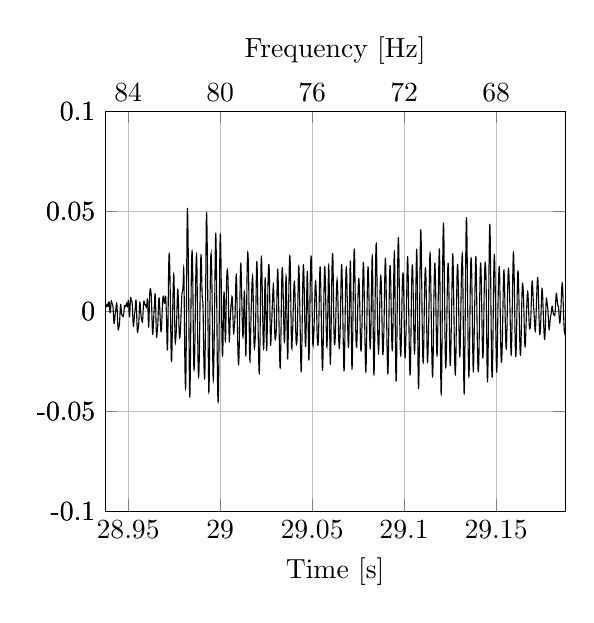
\begin{tikzpicture}


\begin{axis}[%
width=2.3in,
height=2in,
at={(1.011in,0.642in)},
scale only axis,
xmin=28.9375,
xmax=29.1875,
xtick={28.95, 29, 29.05,  29.1, 29.15},
xticklabels={84, 80, 76, 72, 68},
xmajorgrids,
ymin=-0.1,
ymax=0.1,
ymajorgrids,
scaled ticks=false,
ytick={-0.1, -0.05, 0,  0.05, 0.1},
yticklabels={-0.1, -0.05, 0,  0.05, 0.1},
axis x line*=top,
xlabel={Frequency [Hz]},
axis background/.style={fill=white}
]
\end{axis}

\begin{axis}[%
width=2.3in,
height=2in,
at={(1.011in,0.642in)},
scale only axis,
xmin=28.9375,
xmax=29.1875,
xmajorgrids,
ymin=-0.1,
ymax=0.1,
ymajorgrids,
scaled ticks=false,
ytick={-0.1, -0.05, 0,  0.05, 0.1},
yticklabels={-0.1, -0.05, 0,  0.05, 0.1},
xlabel={Time [s]},
axis background/.style={fill=white}
]
\addplot [color=black,solid,forget plot]
table[row sep=crcr]{%
	28.9374791666667	0.00120449066162109\\
	28.9375	0.0013422966003418\\
	28.9375208333333	0.00147902965545654\\
	28.9375416666667	0.00158834457397461\\
	28.9375625	0.00170481204986572\\
	28.9375833333333	0.00182092189788818\\
	28.9376041666667	0.00190639495849609\\
	28.937625	0.00197184085845947\\
	28.9376458333333	0.00206494331359863\\
	28.9376666666667	0.00211882591247559\\
	28.9376875	0.00217843055725098\\
	28.9377083333333	0.00219666957855225\\
	28.9377291666667	0.00223839282989502\\
	28.93775	0.00232481956481934\\
	28.9377708333333	0.00233364105224609\\
	28.9377916666667	0.00235855579376221\\
	28.9378125	0.00237452983856201\\
	28.9378333333333	0.00237023830413818\\
	28.9378541666667	0.00236904621124268\\
	28.937875	0.0023728609085083\\
	28.9378958333333	0.00235486030578613\\
	28.9379166666667	0.00235366821289063\\
	28.9379375	0.00235486030578613\\
	28.9379583333333	0.00233364105224609\\
	28.9379791666667	0.00234019756317139\\
	28.938	0.00231480598449707\\
	28.9380208333333	0.00231778621673584\\
	28.9380416666667	0.00233066082000732\\
	28.9380625	0.00229394435882568\\
	28.9380833333333	0.00233161449432373\\
	28.9381041666667	0.00232195854187012\\
	28.938125	0.00232744216918945\\
	28.9381458333333	0.00236666202545166\\
	28.9381666666667	0.00239074230194092\\
	28.9381875	0.0024111270904541\\
	28.9382083333333	0.00241708755493164\\
	28.9382291666667	0.00250089168548584\\
	28.93825	0.00255060195922852\\
	28.9382708333333	0.00261783599853516\\
	28.9382916666667	0.00265705585479736\\
	28.9383125	0.00270915031433105\\
	28.9383333333333	0.00275206565856934\\
	28.9383541666667	0.00282132625579834\\
	28.938375	0.00291812419891357\\
	28.9383958333333	0.00299406051635742\\
	28.9384166666667	0.00303125381469727\\
	28.9384375	0.00311172008514404\\
	28.9384583333333	0.00321066379547119\\
	28.9384791666667	0.0032811164855957\\
	28.9385	0.00332748889923096\\
	28.9385208333333	0.00336956977844238\\
	28.9385416666667	0.00345480442047119\\
	28.9385625	0.00349807739257813\\
	28.9385833333333	0.00352728366851807\\
	28.9386041666667	0.0035477876663208\\
	28.938625	0.0035707950592041\\
	28.9386458333333	0.00359570980072021\\
	28.9386666666667	0.0036003589630127\\
	28.9386875	0.00357067584991455\\
	28.9387083333333	0.00353062152862549\\
	28.9387291666667	0.00348305702209473\\
	28.93875	0.00348186492919922\\
	28.9387708333333	0.0034555196762085\\
	28.9387916666667	0.00335538387298584\\
	28.9388125	0.00326108932495117\\
	28.9388333333333	0.00318527221679688\\
	28.9388541666667	0.00317442417144775\\
	28.938875	0.00306880474090576\\
	28.9388958333333	0.00293564796447754\\
	28.9389166666667	0.00287473201751709\\
	28.9389375	0.00280296802520752\\
	28.9389583333333	0.00272119045257568\\
	28.9389791666667	0.00266194343566895\\
	28.939	0.00259816646575928\\
	28.9390208333333	0.0025409460067749\\
	28.9390416666667	0.00249350070953369\\
	28.9390625	0.00247383117675781\\
	28.9390833333333	0.00246036052703857\\
	28.9391041666667	0.00245332717895508\\
	28.939125	0.00244832038879395\\
	28.9391458333333	0.00248098373413086\\
	28.9391666666667	0.00252044200897217\\
	28.9391875	0.00253975391387939\\
	28.9392083333333	0.00264823436737061\\
	28.9392291666667	0.00271797180175781\\
	28.93925	0.00281059741973877\\
	28.9392708333333	0.00290811061859131\\
	28.9392916666667	0.00302028656005859\\
	28.9393125	0.00315308570861816\\
	28.9393333333333	0.00329148769378662\\
	28.9393541666667	0.00340831279754639\\
	28.939375	0.00356948375701904\\
	28.9393958333333	0.00372171401977539\\
	28.9394166666667	0.00384736061096191\\
	28.9394375	0.0039832592010498\\
	28.9394583333333	0.00412929058074951\\
	28.9394791666667	0.00424027442932129\\
	28.9395	0.00433218479156494\\
	28.9395208333333	0.00442314147949219\\
	28.9395416666667	0.00449824333190918\\
	28.9395625	0.00455284118652344\\
	28.9395833333333	0.00458669662475586\\
	28.9396041666667	0.0046314001083374\\
	28.939625	0.00459587574005127\\
	28.9396458333333	0.0045621395111084\\
	28.9396666666667	0.00453615188598633\\
	28.9396875	0.0044330358505249\\
	28.9397083333333	0.00432121753692627\\
	28.9397291666667	0.00419533252716064\\
	28.93975	0.00404250621795654\\
	28.9397708333333	0.00387072563171387\\
	28.9397916666667	0.00365662574768066\\
	28.9398125	0.003456711769104\\
	28.9398333333333	0.00322723388671875\\
	28.9398541666667	0.002982497215271\\
	28.939875	0.00272881984710693\\
	28.9398958333333	0.00249087810516357\\
	28.9399166666667	0.00224483013153076\\
	28.9399375	0.00196731090545654\\
	28.9399583333333	0.00170230865478516\\
	28.9399791666667	0.00142776966094971\\
	28.94	0.00115609169006348\\
	28.9400208333333	0.000885367393493652\\
	28.9400416666667	0.000633358955383301\\
	28.9400625	0.000411391258239746\\
	28.9400833333333	0.000180602073669434\\
	28.9401041666667	-8.34465026855469e-06\\
	28.940125	-0.000194072723388672\\
	28.9401458333333	-0.000409603118896484\\
	28.9401666666667	-0.000522017478942871\\
	28.9401875	-0.000576972961425781\\
	28.9402083333333	-0.000643014907836914\\
	28.9402291666667	-0.000677943229675293\\
	28.94025	-0.000661253929138184\\
	28.9402708333333	-0.000652074813842773\\
	28.9402916666667	-0.000607490539550781\\
	28.9403125	-0.000536084175109863\\
	28.9403333333333	-0.000380039215087891\\
	28.9403541666667	-0.000264167785644531\\
	28.940375	-0.00012516975402832\\
	28.9403958333333	1.87158584594727e-05\\
	28.9404166666667	0.000219106674194336\\
	28.9404375	0.000468611717224121\\
	28.9404583333333	0.000717759132385254\\
	28.9404791666667	0.00103902816772461\\
	28.9405	0.00130844116210938\\
	28.9405208333333	0.00157058238983154\\
	28.9405416666667	0.00185871124267578\\
	28.9405625	0.00217807292938232\\
	28.9405833333333	0.00246882438659668\\
	28.9406041666667	0.0027240514755249\\
	28.940625	0.00297737121582031\\
	28.9406458333333	0.00324654579162598\\
	28.9406666666667	0.00350058078765869\\
	28.9406875	0.00375759601593018\\
	28.9407083333333	0.0039670467376709\\
	28.9407291666667	0.00423252582550049\\
	28.94075	0.00441229343414307\\
	28.9407708333333	0.00458657741546631\\
	28.9407916666667	0.00479030609130859\\
	28.9408125	0.00493013858795166\\
	28.9408333333333	0.00502967834472656\\
	28.9408541666667	0.00513112545013428\\
	28.940875	0.00521993637084961\\
	28.9408958333333	0.00522971153259277\\
	28.9409166666667	0.00522172451019287\\
	28.9409375	0.00522911548614502\\
	28.9409583333333	0.00523996353149414\\
	28.9409791666667	0.0052112340927124\\
	28.941	0.00512528419494629\\
	28.9410208333333	0.00503182411193848\\
	28.9410416666667	0.00497424602508545\\
	28.9410625	0.00487077236175537\\
	28.9410833333333	0.00477099418640137\\
	28.9411041666667	0.00464916229248047\\
	28.941125	0.004547119140625\\
	28.9411458333333	0.00443184375762939\\
	28.9411666666667	0.00429177284240723\\
	28.9411875	0.00418353080749512\\
	28.9412083333333	0.00412440299987793\\
	28.9412291666667	0.00401580333709717\\
	28.94125	0.00392568111419678\\
	28.9412708333333	0.00388896465301514\\
	28.9412916666667	0.0037989616394043\\
	28.9413125	0.00372517108917236\\
	28.9413333333333	0.00367295742034912\\
	28.9413541666667	0.00364494323730469\\
	28.941375	0.00362873077392578\\
	28.9413958333333	0.00360417366027832\\
	28.9414166666667	0.00356161594390869\\
	28.9414375	0.00357687473297119\\
	28.9414583333333	0.00352346897125244\\
	28.9414791666667	0.00348567962646484\\
	28.9415	0.00347518920898438\\
	28.9415208333333	0.00347352027893066\\
	28.9415416666667	0.00342643260955811\\
	28.9415625	0.00337326526641846\\
	28.9415833333333	0.00334906578063965\\
	28.9416041666667	0.00328314304351807\\
	28.941625	0.00321304798126221\\
	28.9416458333333	0.00310385227203369\\
	28.9416666666667	0.0030217170715332\\
	28.9416875	0.00289404392242432\\
	28.9417083333333	0.00277328491210938\\
	28.9417291666667	0.00259971618652344\\
	28.94175	0.00243127346038818\\
	28.9417708333333	0.00223422050476074\\
	28.9417916666667	0.00204789638519287\\
	28.9418125	0.00179445743560791\\
	28.9418333333333	0.00156998634338379\\
	28.9418541666667	0.00131797790527344\\
	28.941875	0.00100135803222656\\
	28.9418958333333	0.000730276107788086\\
	28.9419166666667	0.000393033027648926\\
	28.9419375	4.80413436889648e-05\\
	28.9419583333333	-0.000273346900939941\\
	28.9419791666667	-0.000638008117675781\\
	28.942	-0.000986218452453613\\
	28.9420208333333	-0.0013500452041626\\
	28.9420416666667	-0.00172805786132813\\
	28.9420625	-0.00209999084472656\\
	28.9420833333333	-0.00245952606201172\\
	28.9421041666667	-0.00283920764923096\\
	28.942125	-0.00321090221405029\\
	28.9421458333333	-0.00355565547943115\\
	28.9421666666667	-0.00390529632568359\\
	28.9421875	-0.00425815582275391\\
	28.9422083333333	-0.00453579425811768\\
	28.9422291666667	-0.00481522083282471\\
	28.94225	-0.00510096549987793\\
	28.9422708333333	-0.00531721115112305\\
	28.9422916666667	-0.00551402568817139\\
	28.9423125	-0.00571227073669434\\
	28.9423333333333	-0.00587165355682373\\
	28.9423541666667	-0.006011962890625\\
	28.942375	-0.00609862804412842\\
	28.9423958333333	-0.00616216659545898\\
	28.9424166666667	-0.0061640739440918\\
	28.9424375	-0.00617873668670654\\
	28.9424583333333	-0.0061715841293335\\
	28.9424791666667	-0.00609982013702393\\
	28.9425	-0.00601935386657715\\
	28.9425208333333	-0.00593757629394531\\
	28.9425416666667	-0.00584173202514648\\
	28.9425625	-0.00566816329956055\\
	28.9425833333333	-0.00552630424499512\\
	28.9426041666667	-0.00535976886749268\\
	28.942625	-0.00518405437469482\\
	28.9426458333333	-0.00501167774200439\\
	28.9426666666667	-0.00480484962463379\\
	28.9426875	-0.00459206104278564\\
	28.9427083333333	-0.004372239112854\\
	28.9427291666667	-0.00415718555450439\\
	28.94275	-0.00394749641418457\\
	28.9427708333333	-0.00370919704437256\\
	28.9427916666667	-0.00349545478820801\\
	28.9428125	-0.00327563285827637\\
	28.9428333333333	-0.00306379795074463\\
	28.9428541666667	-0.00283503532409668\\
	28.942875	-0.00266897678375244\\
	28.9428958333333	-0.00242698192596436\\
	28.9429166666667	-0.00224006175994873\\
	28.9429375	-0.00203025341033936\\
	28.9429583333333	-0.00185549259185791\\
	28.9429791666667	-0.00171148777008057\\
	28.943	-0.00151622295379639\\
	28.9430208333333	-0.00136935710906982\\
	28.9430416666667	-0.00121152400970459\\
	28.9430625	-0.00106132030487061\\
	28.9430833333333	-0.000919103622436523\\
	28.9431041666667	-0.000782370567321777\\
	28.943125	-0.000638723373413086\\
	28.9431458333333	-0.000498175621032715\\
	28.9431666666667	-0.000345945358276367\\
	28.9431875	-0.000230789184570313\\
	28.9432083333333	-8.38041305541992e-05\\
	28.9432291666667	8.63075256347656e-05\\
	28.94325	0.00023949146270752\\
	28.9432708333333	0.000397205352783203\\
	28.9432916666667	0.000530004501342773\\
	28.9433125	0.000728845596313477\\
	28.9433333333333	0.000880002975463867\\
	28.9433541666667	0.00105178356170654\\
	28.943375	0.00125205516815186\\
	28.9433958333333	0.00144445896148682\\
	28.9434166666667	0.00165307521820068\\
	28.9434375	0.00179791450500488\\
	28.9434583333333	0.00201606750488281\\
	28.9434791666667	0.00223231315612793\\
	28.9435	0.00242531299591064\\
	28.9435208333333	0.00262200832366943\\
	28.9435416666667	0.00280725955963135\\
	28.9435625	0.00299155712127686\\
	28.9435833333333	0.00317680835723877\\
	28.9436041666667	0.00332033634185791\\
	28.943625	0.00349819660186768\\
	28.9436458333333	0.00365996360778809\\
	28.9436666666667	0.00376176834106445\\
	28.9436875	0.0038527250289917\\
	28.9437083333333	0.00394964218139648\\
	28.9437291666667	0.00402390956878662\\
	28.94375	0.00402307510375977\\
	28.9437708333333	0.0040431022644043\\
	28.9437916666667	0.00400960445404053\\
	28.9438125	0.00398123264312744\\
	28.9438333333333	0.00387287139892578\\
	28.9438541666667	0.00376808643341064\\
	28.943875	0.0036466121673584\\
	28.9438958333333	0.00343811511993408\\
	28.9439166666667	0.00322556495666504\\
	28.9439375	0.00299918651580811\\
	28.9439583333333	0.00274956226348877\\
	28.9439791666667	0.00238537788391113\\
	28.944	0.00204110145568848\\
	28.9440208333333	0.00170993804931641\\
	28.9440416666667	0.00127840042114258\\
	28.9440625	0.00086820125579834\\
	28.9440833333333	0.00043022632598877\\
	28.9441041666667	-4.25577163696289e-05\\
	28.944125	-0.000528573989868164\\
	28.9441458333333	-0.000995159149169922\\
	28.9441666666667	-0.00151360034942627\\
	28.9441875	-0.00202596187591553\\
	28.9442083333333	-0.00253725051879883\\
	28.9442291666667	-0.00308370590209961\\
	28.94425	-0.00356650352478027\\
	28.9442708333333	-0.00408291816711426\\
	28.9442916666667	-0.00460159778594971\\
	28.9443125	-0.00507307052612305\\
	28.9443333333333	-0.00550568103790283\\
	28.9443541666667	-0.00596094131469727\\
	28.944375	-0.00639355182647705\\
	28.9443958333333	-0.00678336620330811\\
	28.9444166666667	-0.00715458393096924\\
	28.9444375	-0.00749218463897705\\
	28.9444583333333	-0.00781965255737305\\
	28.9444791666667	-0.00808835029602051\\
	28.9445	-0.00832915306091309\\
	28.9445208333333	-0.00857234001159668\\
	28.9445416666667	-0.0087350606918335\\
	28.9445625	-0.00887703895568848\\
	28.9445833333333	-0.00901639461517334\\
	28.9446041666667	-0.00910532474517822\\
	28.944625	-0.00917530059814453\\
	28.9446458333333	-0.00921499729156494\\
	28.9446666666667	-0.00927221775054932\\
	28.9446875	-0.0092463493347168\\
	28.9447083333333	-0.00926792621612549\\
	28.9447291666667	-0.00922989845275879\\
	28.94475	-0.00919866561889648\\
	28.9447708333333	-0.00914144515991211\\
	28.9447916666667	-0.00907063484191895\\
	28.9448125	-0.00901293754577637\\
	28.9448333333333	-0.00892424583435059\\
	28.9448541666667	-0.00883769989013672\\
	28.944875	-0.00875723361968994\\
	28.9448958333333	-0.00870335102081299\\
	28.9449166666667	-0.0085904598236084\\
	28.9449375	-0.00850820541381836\\
	28.9449583333333	-0.00839269161224365\\
	28.9449791666667	-0.00831711292266846\\
	28.945	-0.0082094669342041\\
	28.9450208333333	-0.00813567638397217\\
	28.9450416666667	-0.00805056095123291\\
	28.9450625	-0.0079272985458374\\
	28.9450833333333	-0.00782966613769531\\
	28.9451041666667	-0.0077434778213501\\
	28.945125	-0.00762271881103516\\
	28.9451458333333	-0.00748217105865479\\
	28.9451666666667	-0.0074012279510498\\
	28.9451875	-0.00725114345550537\\
	28.9452083333333	-0.00711047649383545\\
	28.9452291666667	-0.00694930553436279\\
	28.94525	-0.0067903995513916\\
	28.9452708333333	-0.00657689571380615\\
	28.9452916666667	-0.00638699531555176\\
	28.9453125	-0.00614047050476074\\
	28.9453333333333	-0.00589501857757568\\
	28.9453541666667	-0.00564134120941162\\
	28.945375	-0.00533878803253174\\
	28.9453958333333	-0.0050283670425415\\
	28.9454166666667	-0.0046771764755249\\
	28.9454375	-0.0043487548828125\\
	28.9454583333333	-0.00397193431854248\\
	28.9454791666667	-0.00359225273132324\\
	28.9455	-0.00320053100585938\\
	28.9455208333333	-0.00277113914489746\\
	28.9455416666667	-0.00234317779541016\\
	28.9455625	-0.00193297863006592\\
	28.9455833333333	-0.00148999691009521\\
	28.9456041666667	-0.0010521411895752\\
	28.945625	-0.000657558441162109\\
	28.9456458333333	-0.000228643417358398\\
	28.9456666666667	0.000164389610290527\\
	28.9456875	0.000571966171264648\\
	28.9457083333333	0.000959157943725586\\
	28.9457291666667	0.0012742280960083\\
	28.94575	0.00164806842803955\\
	28.9457708333333	0.00197863578796387\\
	28.9457916666667	0.00224733352661133\\
	28.9458125	0.00248706340789795\\
	28.9458333333333	0.00269651412963867\\
	28.9458541666667	0.00291526317596436\\
	28.945875	0.00307631492614746\\
	28.9458958333333	0.00319766998291016\\
	28.9459166666667	0.00328361988067627\\
	28.9459375	0.00333547592163086\\
	28.9459583333333	0.0033566951751709\\
	28.9459791666667	0.00334405899047852\\
	28.946	0.00330209732055664\\
	28.9460208333333	0.00322556495666504\\
	28.9460416666667	0.00311374664306641\\
	28.9460625	0.00297248363494873\\
	28.9460833333333	0.00281548500061035\\
	28.9461041666667	0.00264823436737061\\
	28.946125	0.00243580341339111\\
	28.9461458333333	0.00223219394683838\\
	28.9461666666667	0.00200450420379639\\
	28.9461875	0.00174605846405029\\
	28.9462083333333	0.00149452686309814\\
	28.9462291666667	0.00123834609985352\\
	28.94625	0.000975608825683594\\
	28.9462708333333	0.000711798667907715\\
	28.9462916666667	0.000437259674072266\\
	28.9463125	0.000186920166015625\\
	28.9463333333333	-4.62532043457031e-05\\
	28.9463541666667	-0.000296592712402344\\
	28.946375	-0.000509381294250488\\
	28.9463958333333	-0.000693798065185547\\
	28.9464166666667	-0.000870347023010254\\
	28.9464375	-0.00106263160705566\\
	28.9464583333333	-0.00124084949493408\\
	28.9464791666667	-0.00135302543640137\\
	28.9465	-0.00150108337402344\\
	28.9465208333333	-0.00159585475921631\\
	28.9465416666667	-0.00174951553344727\\
	28.9465625	-0.00178027153015137\\
	28.9465833333333	-0.00185716152191162\\
	28.9466041666667	-0.00190210342407227\\
	28.946625	-0.00194311141967773\\
	28.9466458333333	-0.00195682048797607\\
	28.9466666666667	-0.00200092792510986\\
	28.9466875	-0.00200068950653076\\
	28.9467083333333	-0.00199317932128906\\
	28.9467291666667	-0.00199985504150391\\
	28.94675	-0.00198268890380859\\
	28.9467708333333	-0.00201892852783203\\
	28.9467916666667	-0.00195181369781494\\
	28.9468125	-0.00197136402130127\\
	28.9468333333333	-0.00197088718414307\\
	28.9468541666667	-0.00195300579071045\\
	28.946875	-0.0019221305847168\\
	28.9468958333333	-0.00193166732788086\\
	28.9469166666667	-0.00193977355957031\\
	28.9469375	-0.00197398662567139\\
	28.9469583333333	-0.00198137760162354\\
	28.9469791666667	-0.00202929973602295\\
	28.947	-0.00204813480377197\\
	28.9470208333333	-0.00205314159393311\\
	28.9470416666667	-0.0021357536315918\\
	28.9470625	-0.00214993953704834\\
	28.9470833333333	-0.0022275447845459\\
	28.9471041666667	-0.00226342678070068\\
	28.947125	-0.0023338794708252\\
	28.9471458333333	-0.0023953914642334\\
	28.9471666666667	-0.00243794918060303\\
	28.9471875	-0.00251471996307373\\
	28.9472083333333	-0.00256145000457764\\
	28.9472291666667	-0.00262069702148438\\
	28.94725	-0.00264477729797363\\
	28.9472708333333	-0.00268018245697021\\
	28.9472916666667	-0.00271868705749512\\
	28.9473125	-0.00275373458862305\\
	28.9473333333333	-0.0027240514755249\\
	28.9473541666667	-0.00271487236022949\\
	28.947375	-0.00269734859466553\\
	28.9473958333333	-0.00266361236572266\\
	28.9474166666667	-0.00259816646575928\\
	28.9474375	-0.00254809856414795\\
	28.9474583333333	-0.0024724006652832\\
	28.9474791666667	-0.00236475467681885\\
	28.9475	-0.00222373008728027\\
	28.9475208333333	-0.00209498405456543\\
	28.9475416666667	-0.00199651718139648\\
	28.9475625	-0.00181496143341064\\
	28.9475833333333	-0.00161874294281006\\
	28.9476041666667	-0.00142979621887207\\
	28.947625	-0.00125586986541748\\
	28.9476458333333	-0.00103628635406494\\
	28.9476666666667	-0.00085151195526123\\
	28.9476875	-0.000629663467407227\\
	28.9477083333333	-0.000427961349487305\\
	28.9477291666667	-0.000189900398254395\\
	28.94775	2.43186950683594e-05\\
	28.9477708333333	0.000212907791137695\\
	28.9477916666667	0.000438451766967773\\
	28.9478125	0.000701308250427246\\
	28.9478333333333	0.000888824462890625\\
	28.9478541666667	0.00107264518737793\\
	28.947875	0.00127303600311279\\
	28.9478958333333	0.00148415565490723\\
	28.9479166666667	0.00163650512695313\\
	28.9479375	0.00178205966949463\\
	28.9479583333333	0.0019611120223999\\
	28.9479791666667	0.00208234786987305\\
	28.948	0.0022122859954834\\
	28.9480208333333	0.00233030319213867\\
	28.9480416666667	0.00245213508605957\\
	28.9480625	0.00254130363464355\\
	28.9480833333333	0.00261390209197998\\
	28.9481041666667	0.00266730785369873\\
	28.948125	0.002768874168396\\
	28.9481458333333	0.00282394886016846\\
	28.9481666666667	0.00283098220825195\\
	28.9481875	0.00286483764648438\\
	28.9482083333333	0.00290322303771973\\
	28.9482291666667	0.00289678573608398\\
	28.94825	0.0028834342956543\\
	28.9482708333333	0.00288903713226318\\
	28.9482916666667	0.00288474559783936\\
	28.9483125	0.00286269187927246\\
	28.9483333333333	0.00282883644104004\\
	28.9483541666667	0.00279414653778076\\
	28.948375	0.00276303291320801\\
	28.9483958333333	0.00272870063781738\\
	28.9484166666667	0.00271797180175781\\
	28.9484375	0.00267577171325684\\
	28.9484583333333	0.00263571739196777\\
	28.9484791666667	0.00257432460784912\\
	28.9485	0.00260186195373535\\
	28.9485208333333	0.00261199474334717\\
	28.9485416666667	0.0025259256362915\\
	28.9485625	0.00253629684448242\\
	28.9485833333333	0.00254309177398682\\
	28.9486041666667	0.00254881381988525\\
	28.948625	0.00251924991607666\\
	28.9486458333333	0.00258731842041016\\
	28.9486666666667	0.0026010274887085\\
	28.9486875	0.00260651111602783\\
	28.9487083333333	0.00261986255645752\\
	28.9487291666667	0.00269746780395508\\
	28.94875	0.00275719165802002\\
	28.9487708333333	0.00278258323669434\\
	28.9487916666667	0.00282752513885498\\
	28.9488125	0.00287473201751709\\
	28.9488333333333	0.00293600559234619\\
	28.9488541666667	0.00301527976989746\\
	28.948875	0.0030893087387085\\
	28.9488958333333	0.00317025184631348\\
	28.9489166666667	0.00324559211730957\\
	28.9489375	0.00328946113586426\\
	28.9489583333333	0.00333797931671143\\
	28.9489791666667	0.00340175628662109\\
	28.949	0.00345754623413086\\
	28.9490208333333	0.00350940227508545\\
	28.9490416666667	0.00359416007995605\\
	28.9490625	0.00362908840179443\\
	28.9490833333333	0.00361824035644531\\
	28.9491041666667	0.0036015510559082\\
	28.949125	0.00365960597991943\\
	28.9491458333333	0.00370883941650391\\
	28.9491666666667	0.00361740589141846\\
	28.9491875	0.00354647636413574\\
	28.9492083333333	0.00355947017669678\\
	28.9492291666667	0.00348484516143799\\
	28.94925	0.00344514846801758\\
	28.9492708333333	0.00336253643035889\\
	28.9492916666667	0.00326979160308838\\
	28.9493125	0.00314474105834961\\
	28.9493333333333	0.00303030014038086\\
	28.9493541666667	0.00299572944641113\\
	28.949375	0.00288474559783936\\
	28.9493958333333	0.00273466110229492\\
	28.9494166666667	0.00265610218048096\\
	28.9494375	0.00257062911987305\\
	28.9494583333333	0.00245749950408936\\
	28.9494791666667	0.00238919258117676\\
	28.9495	0.00232481956481934\\
	28.9495208333333	0.00229990482330322\\
	28.9495416666667	0.00223338603973389\\
	28.9495625	0.002205491065979\\
	28.9495833333333	0.00222384929656982\\
	28.9496041666667	0.00224018096923828\\
	28.949625	0.00226807594299316\\
	28.9496458333333	0.002349853515625\\
	28.9496666666667	0.00245094299316406\\
	28.9496875	0.00250637531280518\\
	28.9497083333333	0.0025869607925415\\
	28.9497291666667	0.00275886058807373\\
	28.94975	0.00294363498687744\\
	28.9497708333333	0.00306534767150879\\
	28.9497916666667	0.00320351123809814\\
	28.9498125	0.00345981121063232\\
	28.9498333333333	0.00364840030670166\\
	28.9498541666667	0.00382018089294434\\
	28.949875	0.00399625301361084\\
	28.9498958333333	0.00420570373535156\\
	28.9499166666667	0.00439226627349854\\
	28.9499375	0.00453698635101318\\
	28.9499583333333	0.0047307014465332\\
	28.9499791666667	0.00490379333496094\\
	28.95	0.00499629974365234\\
	28.9500208333333	0.00507068634033203\\
	28.9500416666667	0.00517380237579346\\
	28.9500625	0.00527513027191162\\
	28.9500833333333	0.00526750087738037\\
	28.9501041666667	0.00522792339324951\\
	28.950125	0.00524055957794189\\
	28.9501458333333	0.00517702102661133\\
	28.9501666666667	0.00502884387969971\\
	28.9501875	0.00488781929016113\\
	28.9502083333333	0.00475656986236572\\
	28.9502291666667	0.00458204746246338\\
	28.95025	0.00433135032653809\\
	28.9502708333333	0.00405228137969971\\
	28.9502916666667	0.00383269786834717\\
	28.9503125	0.00350522994995117\\
	28.9503333333333	0.00316107273101807\\
	28.9503541666667	0.00278890132904053\\
	28.950375	0.00247848033905029\\
	28.9503958333333	0.00213134288787842\\
	28.9504166666667	0.0016934871673584\\
	28.9504375	0.00128757953643799\\
	28.9504583333333	0.000902414321899414\\
	28.9504791666667	0.000477790832519531\\
	28.9505	3.38554382324219e-05\\
	28.9505208333333	-0.000324130058288574\\
	28.9505416666667	-0.000696778297424316\\
	28.9505625	-0.00110518932342529\\
	28.9505833333333	-0.00148618221282959\\
	28.9506041666667	-0.0017240047454834\\
	28.950625	-0.00196230411529541\\
	28.9506458333333	-0.00223922729492188\\
	28.9506666666667	-0.00240206718444824\\
	28.9506875	-0.00247740745544434\\
	28.9507083333333	-0.00260722637176514\\
	28.9507291666667	-0.00270664691925049\\
	28.95075	-0.00269615650177002\\
	28.9507708333333	-0.00262069702148438\\
	28.9507916666667	-0.00257313251495361\\
	28.9508125	-0.0025097131729126\\
	28.9508333333333	-0.00235104560852051\\
	28.9508541666667	-0.00208103656768799\\
	28.950875	-0.00179779529571533\\
	28.9508958333333	-0.00150954723358154\\
	28.9509166666667	-0.00117194652557373\\
	28.9509375	-0.000782370567321777\\
	28.9509583333333	-0.00044858455657959\\
	28.9509791666667	-8.34465026855469e-05\\
	28.951	0.000378012657165527\\
	28.9510208333333	0.000835776329040527\\
	28.9510416666667	0.00127923488616943\\
	28.9510625	0.00171661376953125\\
	28.9510833333333	0.00211620330810547\\
	28.9511041666667	0.00249087810516357\\
	28.951125	0.00293815135955811\\
	28.9511458333333	0.00336539745330811\\
	28.9511666666667	0.00378096103668213\\
	28.9511875	0.00420570373535156\\
	28.9512083333333	0.004599928855896\\
	28.9512291666667	0.00494003295898438\\
	28.95125	0.00526010990142822\\
	28.9512708333333	0.00555706024169922\\
	28.9512916666667	0.00581920146942139\\
	28.9513125	0.00606405735015869\\
	28.9513333333333	0.0062861442565918\\
	28.9513541666667	0.00645327568054199\\
	28.951375	0.00657689571380615\\
	28.9513958333333	0.00669670104980469\\
	28.9514166666667	0.00680875778198242\\
	28.9514375	0.00682854652404785\\
	28.9514583333333	0.00684773921966553\\
	28.9514791666667	0.00681555271148682\\
	28.9515	0.00680291652679443\\
	28.9515208333333	0.00669407844543457\\
	28.9515416666667	0.00658977031707764\\
	28.9515625	0.00653398036956787\\
	28.9515833333333	0.00641906261444092\\
	28.9516041666667	0.00633645057678223\\
	28.951625	0.0062251091003418\\
	28.9516458333333	0.00611782073974609\\
	28.9516666666667	0.00599849224090576\\
	28.9516875	0.00585758686065674\\
	28.9517083333333	0.00576698780059814\\
	28.9517291666667	0.00570058822631836\\
	28.95175	0.00557601451873779\\
	28.9517708333333	0.00548863410949707\\
	28.9517916666667	0.00545024871826172\\
	28.9518125	0.00538110733032227\\
	28.9518333333333	0.0052955150604248\\
	28.9518541666667	0.0052649974822998\\
	28.951875	0.00523805618286133\\
	28.9518958333333	0.00520634651184082\\
	28.9519166666667	0.0051729679107666\\
	28.9519375	0.00515663623809814\\
	28.9519583333333	0.00512909889221191\\
	28.9519791666667	0.00505387783050537\\
	28.952	0.00503396987915039\\
	28.9520208333333	0.0050126314163208\\
	28.9520416666667	0.00497937202453613\\
	28.9520625	0.00488507747650146\\
	28.9520833333333	0.00477564334869385\\
	28.9521041666667	0.00469386577606201\\
	28.952125	0.00460553169250488\\
	28.9521458333333	0.00447690486907959\\
	28.9521666666667	0.00430679321289063\\
	28.9521875	0.00413095951080322\\
	28.9522083333333	0.00396382808685303\\
	28.9522291666667	0.00372219085693359\\
	28.95225	0.00348925590515137\\
	28.9522708333333	0.00323283672332764\\
	28.9522916666667	0.00292778015136719\\
	28.9523125	0.00257265567779541\\
	28.9523333333333	0.00225222110748291\\
	28.9523541666667	0.00188350677490234\\
	28.952375	0.00146079063415527\\
	28.9523958333333	0.00111985206604004\\
	28.9524166666667	0.000669598579406738\\
	28.9524375	0.000219464302062988\\
	28.9524583333333	-0.000203490257263184\\
	28.9524791666667	-0.000688910484313965\\
	28.9525	-0.00115406513214111\\
	28.9525208333333	-0.00164473056793213\\
	28.9525416666667	-0.00214004516601563\\
	28.9525625	-0.00266695022583008\\
	28.9525833333333	-0.00313663482666016\\
	28.9526041666667	-0.00356113910675049\\
	28.952625	-0.00401782989501953\\
	28.9526458333333	-0.00445592403411865\\
	28.9526666666667	-0.00490152835845947\\
	28.9526875	-0.00530540943145752\\
	28.9527083333333	-0.00565338134765625\\
	28.9527291666667	-0.0059959888458252\\
	28.95275	-0.00635015964508057\\
	28.9527708333333	-0.00661516189575195\\
	28.9527916666667	-0.00686180591583252\\
	28.9528125	-0.00709497928619385\\
	28.9528333333333	-0.00728070735931396\\
	28.9528541666667	-0.00741219520568848\\
	28.952875	-0.00749480724334717\\
	28.9528958333333	-0.00756931304931641\\
	28.9529166666667	-0.00758779048919678\\
	28.9529375	-0.00757312774658203\\
	28.9529583333333	-0.00751519203186035\\
	28.9529791666667	-0.00745391845703125\\
	28.953	-0.00731074810028076\\
	28.9530208333333	-0.00720894336700439\\
	28.9530416666667	-0.00704288482666016\\
	28.9530625	-0.00687050819396973\\
	28.9530833333333	-0.00668728351593018\\
	28.9531041666667	-0.00647926330566406\\
	28.953125	-0.00625467300415039\\
	28.9531458333333	-0.00600981712341309\\
	28.9531666666667	-0.00573980808258057\\
	28.9531875	-0.00549042224884033\\
	28.9532083333333	-0.0052182674407959\\
	28.9532291666667	-0.00494956970214844\\
	28.95325	-0.00468552112579346\\
	28.9532708333333	-0.00440812110900879\\
	28.9532916666667	-0.00417304039001465\\
	28.9533125	-0.00392496585845947\\
	28.9533333333333	-0.00367546081542969\\
	28.9533541666667	-0.00341963768005371\\
	28.953375	-0.00317132472991943\\
	28.9533958333333	-0.00293517112731934\\
	28.9534166666667	-0.00268399715423584\\
	28.9534375	-0.00247335433959961\\
	28.9534583333333	-0.00228261947631836\\
	28.9534791666667	-0.00204145908355713\\
	28.9535	-0.00187921524047852\\
	28.9535208333333	-0.00170278549194336\\
	28.9535416666667	-0.00151956081390381\\
	28.9535625	-0.00134849548339844\\
	28.9535833333333	-0.00116229057312012\\
	28.9536041666667	-0.00100100040435791\\
	28.953625	-0.000794291496276855\\
	28.9536458333333	-0.000609517097473145\\
	28.9536666666667	-0.000457167625427246\\
	28.9536875	-0.000290870666503906\\
	28.9537083333333	-6.79492950439453e-05\\
	28.9537291666667	0.000105500221252441\\
	28.95375	0.000274181365966797\\
	28.9537708333333	0.000500321388244629\\
	28.9537916666667	0.000700950622558594\\
	28.9538125	0.000948309898376465\\
	28.9538333333333	0.00116086006164551\\
	28.9538541666667	0.0013805627822876\\
	28.953875	0.00164890289306641\\
	28.9538958333333	0.00190436840057373\\
	28.9539166666667	0.00211906433105469\\
	28.9539375	0.00242495536804199\\
	28.9539583333333	0.00268375873565674\\
	28.9539791666667	0.00295066833496094\\
	28.954	0.00319314002990723\\
	28.9540208333333	0.00344312191009521\\
	28.9540416666667	0.00373101234436035\\
	28.9540625	0.00397837162017822\\
	28.9540833333333	0.00425004959106445\\
	28.9541041666667	0.00446522235870361\\
	28.954125	0.0046539306640625\\
	28.9541458333333	0.0048515796661377\\
	28.9541666666667	0.00503635406494141\\
	28.9541875	0.00519454479217529\\
	28.9542083333333	0.00532019138336182\\
	28.9542291666667	0.00537395477294922\\
	28.95425	0.00546491146087646\\
	28.9542708333333	0.00549256801605225\\
	28.9542916666667	0.00544416904449463\\
	28.9543125	0.00538980960845947\\
	28.9543333333333	0.00531816482543945\\
	28.9543541666667	0.00517880916595459\\
	28.954375	0.0049821138381958\\
	28.9543958333333	0.00475597381591797\\
	28.9544166666667	0.00447738170623779\\
	28.9544375	0.00416076183319092\\
	28.9544583333333	0.00379776954650879\\
	28.9544791666667	0.00340592861175537\\
	28.9545	0.00294911861419678\\
	28.9545208333333	0.00252604484558105\\
	28.9545416666667	0.00204122066497803\\
	28.9545625	0.00148046016693115\\
	28.9545833333333	0.000900387763977051\\
	28.9546041666667	0.000314235687255859\\
	28.954625	-0.000279426574707031\\
	28.9546458333333	-0.000893354415893555\\
	28.9546666666667	-0.00152122974395752\\
	28.9546875	-0.00219964981079102\\
	28.9547083333333	-0.00283873081207275\\
	28.9547291666667	-0.0034942626953125\\
	28.95475	-0.00412964820861816\\
	28.9547708333333	-0.00474798679351807\\
	28.9547916666667	-0.00536942481994629\\
	28.9548125	-0.00594055652618408\\
	28.9548333333333	-0.00648868083953857\\
	28.9548541666667	-0.00704109668731689\\
	28.954875	-0.00754189491271973\\
	28.9548958333333	-0.00797832012176514\\
	28.9549166666667	-0.00843691825866699\\
	28.9549375	-0.00882446765899658\\
	28.9549583333333	-0.00917530059814453\\
	28.9549791666667	-0.00946581363677979\\
	28.955	-0.00973606109619141\\
	28.9550208333333	-0.00999271869659424\\
	28.9550416666667	-0.0101704597473145\\
	28.9550625	-0.0103230476379395\\
	28.9550833333333	-0.0104254484176636\\
	28.9551041666667	-0.0105032920837402\\
	28.955125	-0.0105493068695068\\
	28.9551458333333	-0.0105750560760498\\
	28.9551666666667	-0.0105768442153931\\
	28.9551875	-0.0105404853820801\\
	28.9552083333333	-0.0104724168777466\\
	28.9552291666667	-0.0103836059570313\\
	28.95525	-0.010285496711731\\
	28.9552708333333	-0.0101571083068848\\
	28.9552916666667	-0.0100215673446655\\
	28.9553125	-0.00990748405456543\\
	28.9553333333333	-0.00978660583496094\\
	28.9553541666667	-0.00964224338531494\\
	28.955375	-0.0095217227935791\\
	28.9553958333333	-0.00938808917999268\\
	28.9554166666667	-0.0092320442199707\\
	28.9554375	-0.00913023948669434\\
	28.9554583333333	-0.00894427299499512\\
	28.9554791666667	-0.00882101058959961\\
	28.9555	-0.0086979866027832\\
	28.9555208333333	-0.00857293605804443\\
	28.9555416666667	-0.00847065448760986\\
	28.9555625	-0.00832951068878174\\
	28.9555833333333	-0.0082094669342041\\
	28.9556041666667	-0.00808465480804443\\
	28.955625	-0.00793445110321045\\
	28.9556458333333	-0.00778770446777344\\
	28.9556666666667	-0.0076291561126709\\
	28.9556875	-0.00744998455047607\\
	28.9557083333333	-0.00727570056915283\\
	28.9557291666667	-0.00702822208404541\\
	28.95575	-0.00678634643554688\\
	28.9557708333333	-0.00655519962310791\\
	28.9557916666667	-0.00625503063201904\\
	28.9558125	-0.00593018531799316\\
	28.9558333333333	-0.00559592247009277\\
	28.9558541666667	-0.00524747371673584\\
	28.955875	-0.00481438636779785\\
	28.9558958333333	-0.0044022798538208\\
	28.9559166666667	-0.0039752721786499\\
	28.9559375	-0.00349390506744385\\
	28.9559583333333	-0.00299704074859619\\
	28.9559791666667	-0.00252139568328857\\
	28.956	-0.00204360485076904\\
	28.9560208333333	-0.00151491165161133\\
	28.9560416666667	-0.00101673603057861\\
	28.9560625	-0.000505208969116211\\
	28.9560833333333	-7.15255737304688e-07\\
	28.9561041666667	0.000502347946166992\\
	28.956125	0.000982284545898438\\
	28.9561458333333	0.00147163867950439\\
	28.9561666666667	0.00189208984375\\
	28.9561875	0.00230145454406738\\
	28.9562083333333	0.00271952152252197\\
	28.9562291666667	0.00310266017913818\\
	28.95625	0.00342249870300293\\
	28.9562708333333	0.00370335578918457\\
	28.9562916666667	0.00393462181091309\\
	28.9563125	0.00415194034576416\\
	28.9563333333333	0.00431013107299805\\
	28.9563541666667	0.00444197654724121\\
	28.956375	0.00454044342041016\\
	28.9563958333333	0.00458753108978271\\
	28.9564166666667	0.0045846700668335\\
	28.9564375	0.00454378128051758\\
	28.9564583333333	0.00447869300842285\\
	28.9564791666667	0.00437462329864502\\
	28.9565	0.00427126884460449\\
	28.9565208333333	0.00410723686218262\\
	28.9565416666667	0.00391364097595215\\
	28.9565625	0.00366950035095215\\
	28.9565833333333	0.00344395637512207\\
	28.9566041666667	0.00315606594085693\\
	28.956625	0.0028681755065918\\
	28.9566458333333	0.00257217884063721\\
	28.9566666666667	0.00225400924682617\\
	28.9566875	0.00198066234588623\\
	28.9567083333333	0.00165057182312012\\
	28.9567291666667	0.00133812427520752\\
	28.95675	0.00105643272399902\\
	28.9567708333333	0.000751376152038574\\
	28.9567916666667	0.000424861907958984\\
	28.9568125	0.000171065330505371\\
	28.9568333333333	-9.0479850769043e-05\\
	28.9568541666667	-0.000412583351135254\\
	28.956875	-0.000677227973937988\\
	28.9568958333333	-0.000899434089660645\\
	28.9569166666667	-0.00112056732177734\\
	28.9569375	-0.00137567520141602\\
	28.9569583333333	-0.00157546997070313\\
	28.9569791666667	-0.00175034999847412\\
	28.957	-0.00192892551422119\\
	28.9570208333333	-0.00210666656494141\\
	28.9570416666667	-0.00226378440856934\\
	28.9570625	-0.00239062309265137\\
	28.9570833333333	-0.00253975391387939\\
	28.9571041666667	-0.00269770622253418\\
	28.957125	-0.00281667709350586\\
	28.9571458333333	-0.0028921365737915\\
	28.9571666666667	-0.00301814079284668\\
	28.9571875	-0.00316214561462402\\
	28.9572083333333	-0.00325405597686768\\
	28.9572291666667	-0.00332438945770264\\
	28.95725	-0.00347423553466797\\
	28.9572708333333	-0.00358736515045166\\
	28.9572916666667	-0.00364816188812256\\
	28.9573125	-0.00376880168914795\\
	28.9573333333333	-0.00388860702514648\\
	28.9573541666667	-0.00401592254638672\\
	28.957375	-0.00411760807037354\\
	28.9573958333333	-0.00422906875610352\\
	28.9574166666667	-0.00434303283691406\\
	28.9574375	-0.00446224212646484\\
	28.9574583333333	-0.00459122657775879\\
	28.9574791666667	-0.00470340251922607\\
	28.9575	-0.00483143329620361\\
	28.9575208333333	-0.00491082668304443\\
	28.9575416666667	-0.00500977039337158\\
	28.9575625	-0.00514519214630127\\
	28.9575833333333	-0.0052182674407959\\
	28.9576041666667	-0.00528013706207275\\
	28.957625	-0.00533974170684814\\
	28.9576458333333	-0.00541150569915771\\
	28.9576666666667	-0.0054318904876709\\
	28.9576875	-0.00544106960296631\\
	28.9577083333333	-0.00546121597290039\\
	28.9577291666667	-0.00540852546691895\\
	28.95775	-0.00538194179534912\\
	28.9577708333333	-0.0053030252456665\\
	28.9577916666667	-0.00520288944244385\\
	28.9578125	-0.00511598587036133\\
	28.9578333333333	-0.00496828556060791\\
	28.9578541666667	-0.00479567050933838\\
	28.957875	-0.00462913513183594\\
	28.9578958333333	-0.00439846515655518\\
	28.9579166666667	-0.00417149066925049\\
	28.9579375	-0.00386989116668701\\
	28.9579583333333	-0.00359725952148438\\
	28.9579791666667	-0.00328981876373291\\
	28.958	-0.0029522180557251\\
	28.9580208333333	-0.00262069702148438\\
	28.9580416666667	-0.00224769115447998\\
	28.9580625	-0.00188589096069336\\
	28.9580833333333	-0.0014883279800415\\
	28.9581041666667	-0.00112724304199219\\
	28.958125	-0.000753998756408691\\
	28.9581458333333	-0.000306248664855957\\
	28.9581666666667	8.85725021362305e-05\\
	28.9581875	0.000467658042907715\\
	28.9582083333333	0.000868678092956543\\
	28.9582291666667	0.00126349925994873\\
	28.95825	0.00159382820129395\\
	28.9582708333333	0.00193023681640625\\
	28.9582916666667	0.0022960901260376\\
	28.9583125	0.00263822078704834\\
	28.9583333333333	0.00293898582458496\\
	28.9583541666667	0.00319647789001465\\
	28.958375	0.00343501567840576\\
	28.9583958333333	0.00368666648864746\\
	28.9584166666667	0.0039290189743042\\
	28.9584375	0.00411438941955566\\
	28.9584583333333	0.00428915023803711\\
	28.9584791666667	0.00444447994232178\\
	28.9585	0.00455582141876221\\
	28.9585208333333	0.00466132164001465\\
	28.9585416666667	0.00477266311645508\\
	28.9585625	0.00482368469238281\\
	28.9585833333333	0.00485706329345703\\
	28.9586041666667	0.00491297245025635\\
	28.958625	0.00495719909667969\\
	28.9586458333333	0.00490915775299072\\
	28.9586666666667	0.00486946105957031\\
	28.9586875	0.00485026836395264\\
	28.9587083333333	0.00480246543884277\\
	28.9587291666667	0.00474405288696289\\
	28.95875	0.00468635559082031\\
	28.9587708333333	0.00462841987609863\\
	28.9587916666667	0.00449824333190918\\
	28.9588125	0.00438845157623291\\
	28.9588333333333	0.00435793399810791\\
	28.9588541666667	0.00428080558776855\\
	28.958875	0.0041424036026001\\
	28.9588958333333	0.00405645370483398\\
	28.9589166666667	0.00400471687316895\\
	28.9589375	0.00390815734863281\\
	28.9589583333333	0.00382733345031738\\
	28.9589791666667	0.00376176834106445\\
	28.959	0.00368845462799072\\
	28.9590208333333	0.00362837314605713\\
	28.9590416666667	0.00353908538818359\\
	28.9590625	0.00352597236633301\\
	28.9590833333333	0.00348150730133057\\
	28.9591041666667	0.00338888168334961\\
	28.959125	0.00334370136260986\\
	28.9591458333333	0.00332820415496826\\
	28.9591666666667	0.00326156616210938\\
	28.9591875	0.00322854518890381\\
	28.9592083333333	0.00319218635559082\\
	28.9592291666667	0.00316357612609863\\
	28.95925	0.0031430721282959\\
	28.9592708333333	0.00309181213378906\\
	28.9592916666667	0.00307798385620117\\
	28.9593125	0.00307083129882813\\
	28.9593333333333	0.00307929515838623\\
	28.9593541666667	0.00302028656005859\\
	28.959375	0.00298082828521729\\
	28.9593958333333	0.00300610065460205\\
	28.9594166666667	0.00300836563110352\\
	28.9594375	0.00296783447265625\\
	28.9594583333333	0.00297856330871582\\
	28.9594791666667	0.00301039218902588\\
	28.9595	0.00296151638031006\\
	28.9595208333333	0.00294613838195801\\
	28.9595416666667	0.00297081470489502\\
	28.9595625	0.00295579433441162\\
	28.9595833333333	0.00286734104156494\\
	28.9596041666667	0.0028759241104126\\
	28.959625	0.00288176536560059\\
	28.9596458333333	0.00281000137329102\\
	28.9596666666667	0.00275087356567383\\
	28.9596875	0.00270700454711914\\
	28.9597083333333	0.00270462036132813\\
	28.9597291666667	0.0026094913482666\\
	28.95975	0.00251424312591553\\
	28.9597708333333	0.00248515605926514\\
	28.9597916666667	0.00244176387786865\\
	28.9598125	0.00230515003204346\\
	28.9598333333333	0.00226759910583496\\
	28.9598541666667	0.00228989124298096\\
	28.959875	0.00221312046051025\\
	28.9598958333333	0.00210249423980713\\
	28.9599166666667	0.00208449363708496\\
	28.9599375	0.0022047758102417\\
	28.9599583333333	0.00214290618896484\\
	28.9599791666667	0.00208067893981934\\
	28.96	0.00213503837585449\\
	28.9600208333333	0.00225937366485596\\
	28.9600416666667	0.00232577323913574\\
	28.9600625	0.00237166881561279\\
	28.9600833333333	0.00248968601226807\\
	28.9601041666667	0.00265204906463623\\
	28.960125	0.00277423858642578\\
	28.9601458333333	0.00292432308197021\\
	28.9601666666667	0.00315630435943604\\
	28.9601875	0.00336587429046631\\
	28.9602083333333	0.00355863571166992\\
	28.9602291666667	0.00375306606292725\\
	28.96025	0.0039900541305542\\
	28.9602708333333	0.00423324108123779\\
	28.9602916666667	0.00445401668548584\\
	28.9603125	0.00469350814819336\\
	28.9603333333333	0.00496053695678711\\
	28.9603541666667	0.00517582893371582\\
	28.960375	0.00533473491668701\\
	28.9603958333333	0.00551259517669678\\
	28.9604166666667	0.00574064254760742\\
	28.9604375	0.0058741569519043\\
	28.9604583333333	0.00594353675842285\\
	28.9604791666667	0.0060044527053833\\
	28.9605	0.00608706474304199\\
	28.9605208333333	0.00607001781463623\\
	28.9605416666667	0.00602066516876221\\
	28.9605625	0.00594222545623779\\
	28.9605833333333	0.00582301616668701\\
	28.9606041666667	0.00564396381378174\\
	28.960625	0.00539326667785645\\
	28.9606458333333	0.00517582893371582\\
	28.9606666666667	0.00482869148254395\\
	28.9606875	0.0044102668762207\\
	28.9607083333333	0.00404214859008789\\
	28.9607291666667	0.00359189510345459\\
	28.96075	0.00300586223602295\\
	28.9607708333333	0.00237274169921875\\
	28.9607916666667	0.00178325176239014\\
	28.9608125	0.00113105773925781\\
	28.9608333333333	0.000365495681762695\\
	28.9608541666667	-0.000380992889404297\\
	28.960875	-0.00107312202453613\\
	28.9608958333333	-0.0018237829208374\\
	28.9609166666667	-0.00260269641876221\\
	28.9609375	-0.00324511528015137\\
	28.9609583333333	-0.00386106967926025\\
	28.9609791666667	-0.0044701099395752\\
	28.961	-0.00507402420043945\\
	28.9610208333333	-0.0055617094039917\\
	28.9610416666667	-0.00603234767913818\\
	28.9610625	-0.006522536277771\\
	28.9610833333333	-0.00686502456665039\\
	28.9611041666667	-0.00710511207580566\\
	28.961125	-0.00736713409423828\\
	28.9611458333333	-0.00761115550994873\\
	28.9611666666667	-0.00773429870605469\\
	28.9611875	-0.00770509243011475\\
	28.9612083333333	-0.00755345821380615\\
	28.9612291666667	-0.00736665725708008\\
	28.96125	-0.00708878040313721\\
	28.9612708333333	-0.00673317909240723\\
	28.9612916666667	-0.00633609294891357\\
	28.9613125	-0.00583922863006592\\
	28.9613333333333	-0.00528120994567871\\
	28.9613541666667	-0.0047447681427002\\
	28.961375	-0.00417983531951904\\
	28.9613958333333	-0.00353050231933594\\
	28.9614166666667	-0.00286877155303955\\
	28.9614375	-0.00218379497528076\\
	28.9614583333333	-0.00142109394073486\\
	28.9614791666667	-0.000641703605651855\\
	28.9615	9.97781753540039e-05\\
	28.9615208333333	0.000829935073852539\\
	28.9615416666667	0.00164186954498291\\
	28.9615625	0.00244879722595215\\
	28.9615833333333	0.00325644016265869\\
	28.9616041666667	0.00396919250488281\\
	28.961625	0.00461471080780029\\
	28.9616458333333	0.00522804260253906\\
	28.9616666666667	0.00587832927703857\\
	28.9616875	0.00651669502258301\\
	28.9617083333333	0.00711798667907715\\
	28.9617291666667	0.0077364444732666\\
	28.96175	0.00827920436859131\\
	28.9617708333333	0.00874865055084229\\
	28.9617916666667	0.00913190841674805\\
	28.9618125	0.00951623916625977\\
	28.9618333333333	0.00974369049072266\\
	28.9618541666667	0.0100182294845581\\
	28.961875	0.0102889537811279\\
	28.9618958333333	0.0104821920394897\\
	28.9619166666667	0.0106514692306519\\
	28.9619375	0.0107780694961548\\
	28.9619583333333	0.0109632015228271\\
	28.9619791666667	0.0110411643981934\\
	28.962	0.0110743045806885\\
	28.9620208333333	0.0110816955566406\\
	28.9620416666667	0.0111067295074463\\
	28.9620625	0.0110859870910645\\
	28.9620833333333	0.0110983848571777\\
	28.9621041666667	0.0110651254653931\\
	28.962125	0.0109924077987671\\
	28.9621458333333	0.0109944343566895\\
	28.9621666666667	0.0109552145004272\\
	28.9621875	0.0109134912490845\\
	28.9622083333333	0.0108917951583862\\
	28.9622291666667	0.010913610458374\\
	28.96225	0.0108722448348999\\
	28.9622708333333	0.010759711265564\\
	28.9622916666667	0.0106019973754883\\
	28.9623125	0.0104871988296509\\
	28.9623333333333	0.0103648900985718\\
	28.9623541666667	0.0102463960647583\\
	28.962375	0.0101308822631836\\
	28.9623958333333	0.0099644660949707\\
	28.9624166666667	0.00979447364807129\\
	28.9624375	0.00957882404327393\\
	28.9624583333333	0.00943195819854736\\
	28.9624791666667	0.00923633575439453\\
	28.9625	0.00898420810699463\\
	28.9625208333333	0.00874018669128418\\
	28.9625416666667	0.00848448276519775\\
	28.9625625	0.00819408893585205\\
	28.9625833333333	0.00786113739013672\\
	28.9626041666667	0.00750446319580078\\
	28.962625	0.0071481466293335\\
	28.9626458333333	0.00675618648529053\\
	28.9626666666667	0.00633704662322998\\
	28.9626875	0.00586175918579102\\
	28.9627083333333	0.00536429882049561\\
	28.9627291666667	0.00485575199127197\\
	28.96275	0.00428462028503418\\
	28.9627708333333	0.00372755527496338\\
	28.9627916666667	0.0031510591506958\\
	28.9628125	0.00251221656799316\\
	28.9628333333333	0.00184381008148193\\
	28.9628541666667	0.00115585327148438\\
	28.962875	0.000433921813964844\\
	28.9628958333333	-0.000317096710205078\\
	28.9629166666667	-0.00104808807373047\\
	28.9629375	-0.00179862976074219\\
	28.9629583333333	-0.00253081321716309\\
	28.9629791666667	-0.00321769714355469\\
	28.963	-0.00393152236938477\\
	28.9630208333333	-0.00464785099029541\\
	28.9630416666667	-0.00532877445220947\\
	28.9630625	-0.00601720809936523\\
	28.9630833333333	-0.0066368579864502\\
	28.9631041666667	-0.00727307796478271\\
	28.963125	-0.00782561302185059\\
	28.9631458333333	-0.00835847854614258\\
	28.9631666666667	-0.00887608528137207\\
	28.9631875	-0.00934088230133057\\
	28.9632083333333	-0.00979912281036377\\
	28.9632291666667	-0.0101571083068848\\
	28.96325	-0.0105267763137817\\
	28.9632708333333	-0.0108393430709839\\
	28.9632916666667	-0.0110433101654053\\
	28.9633125	-0.0112289190292358\\
	28.9633333333333	-0.0113974809646606\\
	28.9633541666667	-0.0114800930023193\\
	28.963375	-0.0115460157394409\\
	28.9633958333333	-0.0115615129470825\\
	28.9634166666667	-0.0115418434143066\\
	28.9634375	-0.0114400386810303\\
	28.9634583333333	-0.0112873315811157\\
	28.9634791666667	-0.0111125707626343\\
	28.9635	-0.0108804702758789\\
	28.9635208333333	-0.0106531381607056\\
	28.9635416666667	-0.0103731155395508\\
	28.9635625	-0.0100827217102051\\
	28.9635833333333	-0.009757399559021\\
	28.9636041666667	-0.00942695140838623\\
	28.963625	-0.00905096530914307\\
	28.9636458333333	-0.00866913795471191\\
	28.9636666666667	-0.00826072692871094\\
	28.9636875	-0.0078510046005249\\
	28.9637083333333	-0.00742387771606445\\
	28.9637291666667	-0.00699269771575928\\
	28.96375	-0.00658059120178223\\
	28.9637708333333	-0.00614070892333984\\
	28.9637916666667	-0.00573277473449707\\
	28.9638125	-0.00529623031616211\\
	28.9638333333333	-0.0048907995223999\\
	28.9638541666667	-0.00449824333190918\\
	28.963875	-0.00413179397583008\\
	28.9638958333333	-0.00376057624816895\\
	28.9639166666667	-0.00336456298828125\\
	28.9639375	-0.00297808647155762\\
	28.9639583333333	-0.00260758399963379\\
	28.9639791666667	-0.00223791599273682\\
	28.964	-0.00186991691589355\\
	28.9640208333333	-0.00151669979095459\\
	28.9640416666667	-0.00112974643707275\\
	28.9640625	-0.000795602798461914\\
	28.9640833333333	-0.000431299209594727\\
	28.9641041666667	-6.49690628051758e-05\\
	28.964125	0.000289559364318848\\
	28.9641458333333	0.000647187232971191\\
	28.9641666666667	0.00101220607757568\\
	28.9641875	0.00138700008392334\\
	28.9642083333333	0.00174784660339355\\
	28.9642291666667	0.00211501121520996\\
	28.96425	0.00250840187072754\\
	28.9642708333333	0.00291848182678223\\
	28.9642916666667	0.00326371192932129\\
	28.9643125	0.00364780426025391\\
	28.9643333333333	0.00409185886383057\\
	28.9643541666667	0.00444722175598145\\
	28.964375	0.00484919548034668\\
	28.9643958333333	0.00522089004516602\\
	28.9644166666667	0.00562143325805664\\
	28.9644375	0.0059809684753418\\
	28.9644583333333	0.00632774829864502\\
	28.9644791666667	0.00670421123504639\\
	28.9645	0.00705075263977051\\
	28.9645208333333	0.00736451148986816\\
	28.9645416666667	0.0076298713684082\\
	28.9645625	0.00789988040924072\\
	28.9645833333333	0.0081489086151123\\
	28.9646041666667	0.00833797454833984\\
	28.964625	0.00842487812042236\\
	28.9646458333333	0.00855910778045654\\
	28.9646666666667	0.00862300395965576\\
	28.9646875	0.00860285758972168\\
	28.9647083333333	0.00855171680450439\\
	28.9647291666667	0.0084681510925293\\
	28.96475	0.00831079483032227\\
	28.9647708333333	0.00807297229766846\\
	28.9647916666667	0.00784409046173096\\
	28.9648125	0.0075230598449707\\
	28.9648333333333	0.00713801383972168\\
	28.9648541666667	0.00669360160827637\\
	28.964875	0.00623607635498047\\
	28.9648958333333	0.00567865371704102\\
	28.9649166666667	0.0050806999206543\\
	28.9649375	0.00442898273468018\\
	28.9649583333333	0.00373542308807373\\
	28.9649791666667	0.0030057430267334\\
	28.965	0.00221335887908936\\
	28.9650208333333	0.00139617919921875\\
	28.9650416666667	0.000580310821533203\\
	28.9650625	-0.000258684158325195\\
	28.9650833333333	-0.00115859508514404\\
	28.9651041666667	-0.00202059745788574\\
	28.965125	-0.00290346145629883\\
	28.9651458333333	-0.00378811359405518\\
	28.9651666666667	-0.00464379787445068\\
	28.9651875	-0.00550627708435059\\
	28.9652083333333	-0.00634109973907471\\
	28.9652291666667	-0.00718939304351807\\
	28.96525	-0.00792813301086426\\
	28.9652708333333	-0.00865411758422852\\
	28.9652916666667	-0.00935721397399902\\
	28.9653125	-0.00998938083648682\\
	28.9653333333333	-0.0105630159378052\\
	28.9653541666667	-0.0110820531845093\\
	28.965375	-0.0115711688995361\\
	28.9653958333333	-0.0119649171829224\\
	28.9654166666667	-0.0122936964035034\\
	28.9654375	-0.0125917196273804\\
	28.9654583333333	-0.0128222703933716\\
	28.9654791666667	-0.0129580497741699\\
	28.9655	-0.0130702257156372\\
	28.9655208333333	-0.0131006240844727\\
	28.9655416666667	-0.0130939483642578\\
	28.9655625	-0.0130192041397095\\
	28.9655833333333	-0.0129015445709229\\
	28.9656041666667	-0.0127681493759155\\
	28.965625	-0.0125608444213867\\
	28.9656458333333	-0.0123584270477295\\
	28.9656666666667	-0.0121055841445923\\
	28.9656875	-0.0118530988693237\\
	28.9657083333333	-0.0115878582000732\\
	28.9657291666667	-0.0113177299499512\\
	28.96575	-0.0110512971878052\\
	28.9657708333333	-0.0107724666595459\\
	28.9657916666667	-0.0104954242706299\\
	28.9658125	-0.0102572441101074\\
	28.9658333333333	-0.0100201368331909\\
	28.9658541666667	-0.00978457927703857\\
	28.965875	-0.00958037376403809\\
	28.9658958333333	-0.00936806201934814\\
	28.9659166666667	-0.00918698310852051\\
	28.9659375	-0.00896203517913818\\
	28.9659583333333	-0.00878238677978516\\
	28.9659791666667	-0.00860404968261719\\
	28.966	-0.00839293003082275\\
	28.9660208333333	-0.00822246074676514\\
	28.9660416666667	-0.0079578161239624\\
	28.9660625	-0.00772297382354736\\
	28.9660833333333	-0.0074923038482666\\
	28.9661041666667	-0.00719273090362549\\
	28.966125	-0.00689399242401123\\
	28.9661458333333	-0.00653207302093506\\
	28.9661666666667	-0.00615835189819336\\
	28.9661875	-0.00577354431152344\\
	28.9662083333333	-0.00534605979919434\\
	28.9662291666667	-0.00487375259399414\\
	28.96625	-0.00440549850463867\\
	28.9662708333333	-0.00391602516174316\\
	28.9662916666667	-0.00339531898498535\\
	28.9663125	-0.00286853313446045\\
	28.9663333333333	-0.00231897830963135\\
	28.9663541666667	-0.00176560878753662\\
	28.966375	-0.00119900703430176\\
	28.9663958333333	-0.000627398490905762\\
	28.9664166666667	-4.72068786621094e-05\\
	28.9664375	0.000533223152160645\\
	28.9664583333333	0.00111520290374756\\
	28.9664791666667	0.00166141986846924\\
	28.9665	0.0022042989730835\\
	28.9665208333333	0.00276672840118408\\
	28.9665416666667	0.00325405597686768\\
	28.9665625	0.00374341011047363\\
	28.9665833333333	0.00420749187469482\\
	28.9666041666667	0.00462758541107178\\
	28.966625	0.00502431392669678\\
	28.9666458333333	0.00536978244781494\\
	28.9666666666667	0.00570642948150635\\
	28.9666875	0.0059974193572998\\
	28.9667083333333	0.00622272491455078\\
	28.9667291666667	0.00638663768768311\\
	28.96675	0.00653302669525146\\
	28.9667708333333	0.00664234161376953\\
	28.9667916666667	0.00670492649078369\\
	28.9668125	0.0067136287689209\\
	28.9668333333333	0.00667774677276611\\
	28.9668541666667	0.00662362575531006\\
	28.966875	0.00651395320892334\\
	28.9668958333333	0.00637960433959961\\
	28.9669166666667	0.00621557235717773\\
	28.9669375	0.0059969425201416\\
	28.9669583333333	0.00575816631317139\\
	28.9669791666667	0.00548946857452393\\
	28.967	0.00521552562713623\\
	28.9670208333333	0.00489163398742676\\
	28.9670416666667	0.00453627109527588\\
	28.9670625	0.00419604778289795\\
	28.9670833333333	0.00387704372406006\\
	28.9671041666667	0.00347304344177246\\
	28.967125	0.00308537483215332\\
	28.9671458333333	0.00272238254547119\\
	28.9671666666667	0.0023190975189209\\
	28.9671875	0.00185680389404297\\
	28.9672083333333	0.00143039226531982\\
	28.9672291666667	0.00101888179779053\\
	28.96725	0.000579953193664551\\
	28.9672708333333	7.79628753662109e-05\\
	28.9672916666667	-0.000388503074645996\\
	28.9673125	-0.000801801681518555\\
	28.9673333333333	-0.00127208232879639\\
	28.9673541666667	-0.00177156925201416\\
	28.967375	-0.00222182273864746\\
	28.9673958333333	-0.00262594223022461\\
	28.9674166666667	-0.00313079357147217\\
	28.9674375	-0.00360608100891113\\
	28.9674583333333	-0.0040050745010376\\
	28.9674791666667	-0.00443267822265625\\
	28.9675	-0.00490069389343262\\
	28.9675208333333	-0.00533890724182129\\
	28.9675416666667	-0.00568687915802002\\
	28.9675625	-0.00610494613647461\\
	28.9675833333333	-0.0065692663192749\\
	28.9676041666667	-0.00691473484039307\\
	28.967625	-0.00723433494567871\\
	28.9676458333333	-0.00760853290557861\\
	28.9676666666667	-0.00798952579498291\\
	28.9676875	-0.00825870037078857\\
	28.9677083333333	-0.00854241847991943\\
	28.9677291666667	-0.00889754295349121\\
	28.96775	-0.0091547966003418\\
	28.9677708333333	-0.00931310653686523\\
	28.9677916666667	-0.00951910018920898\\
	28.9678125	-0.00976061820983887\\
	28.9678333333333	-0.00989747047424316\\
	28.9678541666667	-0.00999009609222412\\
	28.967875	-0.01012122631073\\
	28.9678958333333	-0.0102109909057617\\
	28.9679166666667	-0.0102143287658691\\
	28.9679375	-0.0102025270462036\\
	28.9679583333333	-0.0102142095565796\\
	28.9679791666667	-0.0101821422576904\\
	28.968	-0.0100768804550171\\
	28.9680208333333	-0.00994348526000977\\
	28.9680416666667	-0.00983631610870361\\
	28.9680625	-0.00967097282409668\\
	28.9680833333333	-0.00944244861602783\\
	28.9681041666667	-0.00920164585113525\\
	28.968125	-0.00896036624908447\\
	28.9681458333333	-0.00868415832519531\\
	28.9681666666667	-0.00834083557128906\\
	28.9681875	-0.00799572467803955\\
	28.9682083333333	-0.00765776634216309\\
	28.9682291666667	-0.00725030899047852\\
	28.96825	-0.00677788257598877\\
	28.9682708333333	-0.00639081001281738\\
	28.9682916666667	-0.00594460964202881\\
	28.9683125	-0.0054619312286377\\
	28.9683333333333	-0.00494742393493652\\
	28.9683541666667	-0.00449347496032715\\
	28.968375	-0.00399506092071533\\
	28.9683958333333	-0.00343382358551025\\
	28.9684166666667	-0.00289309024810791\\
	28.9684375	-0.00239980220794678\\
	28.9684583333333	-0.00186741352081299\\
	28.9684791666667	-0.00131094455718994\\
	28.9685	-0.000799775123596191\\
	28.9685208333333	-0.000259995460510254\\
	28.9685416666667	0.000267386436462402\\
	28.9685625	0.000778675079345703\\
	28.9685833333333	0.0012662410736084\\
	28.9686041666667	0.00172436237335205\\
	28.968625	0.00222337245941162\\
	28.9686458333333	0.00269615650177002\\
	28.9686666666667	0.00310921669006348\\
	28.9686875	0.0035393238067627\\
	28.9687083333333	0.00395631790161133\\
	28.9687291666667	0.00430595874786377\\
	28.96875	0.0046546459197998\\
	28.9687708333333	0.00497937202453613\\
	28.9687916666667	0.00530338287353516\\
	28.9688125	0.00561881065368652\\
	28.9688333333333	0.00590312480926514\\
	28.9688541666667	0.00613701343536377\\
	28.968875	0.0063631534576416\\
	28.9688958333333	0.00657021999359131\\
	28.9689166666667	0.00674545764923096\\
	28.9689375	0.0069202184677124\\
	28.9689583333333	0.00707054138183594\\
	28.9689791666667	0.00718569755554199\\
	28.969	0.00724279880523682\\
	28.9690208333333	0.00732779502868652\\
	28.9690416666667	0.00738096237182617\\
	28.9690625	0.00744295120239258\\
	28.9690833333333	0.0074160099029541\\
	28.9691041666667	0.00740683078765869\\
	28.969125	0.0073779821395874\\
	28.9691458333333	0.00733113288879395\\
	28.9691666666667	0.00726354122161865\\
	28.9691875	0.00718140602111816\\
	28.9692083333333	0.00712418556213379\\
	28.9692291666667	0.00697195529937744\\
	28.96925	0.0068352222442627\\
	28.9692708333333	0.00675797462463379\\
	28.9692916666667	0.00661599636077881\\
	28.9693125	0.00641369819641113\\
	28.9693333333333	0.00628113746643066\\
	28.9693541666667	0.00617623329162598\\
	28.969375	0.00604701042175293\\
	28.9693958333333	0.00584912300109863\\
	28.9694166666667	0.0056769847869873\\
	28.9694375	0.00556886196136475\\
	28.9694583333333	0.00541245937347412\\
	28.9694791666667	0.00521302223205566\\
	28.9695	0.00509274005889893\\
	28.9695208333333	0.00498974323272705\\
	28.9695416666667	0.0048375129699707\\
	28.9695625	0.0046766996383667\\
	28.9695833333333	0.00457084178924561\\
	28.9696041666667	0.00447475910186768\\
	28.969625	0.00436305999755859\\
	28.9696458333333	0.00428366661071777\\
	28.9696666666667	0.0042649507522583\\
	28.9696875	0.00421774387359619\\
	28.9697083333333	0.00408387184143066\\
	28.9697291666667	0.00409555435180664\\
	28.96975	0.00415647029876709\\
	28.9697708333333	0.00416398048400879\\
	28.9697916666667	0.0041424036026001\\
	28.9698125	0.00416982173919678\\
	28.9698333333333	0.00434541702270508\\
	28.9698541666667	0.00441634654998779\\
	28.969875	0.00440633296966553\\
	28.9698958333333	0.0045311450958252\\
	28.9699166666667	0.00474190711975098\\
	28.9699375	0.00486588478088379\\
	28.9699583333333	0.00498008728027344\\
	28.9699791666667	0.00514626502990723\\
	28.97	0.00533771514892578\\
	28.9700208333333	0.00548911094665527\\
	28.9700416666667	0.005668044090271\\
	28.9700625	0.00585842132568359\\
	28.9700833333333	0.00596857070922852\\
	28.9701041666667	0.00610792636871338\\
	28.970125	0.00633978843688965\\
	28.9701458333333	0.00657308101654053\\
	28.9701666666667	0.00668990612030029\\
	28.9701875	0.00677037239074707\\
	28.9702083333333	0.00695455074310303\\
	28.9702291666667	0.00715482234954834\\
	28.97025	0.00724649429321289\\
	28.9702708333333	0.00732827186584473\\
	28.9702916666667	0.00742042064666748\\
	28.9703125	0.00746893882751465\\
	28.9703333333333	0.00746607780456543\\
	28.9703541666667	0.00746476650238037\\
	28.970375	0.00744509696960449\\
	28.9703958333333	0.00730407238006592\\
	28.9704166666667	0.00710010528564453\\
	28.9704375	0.00699996948242188\\
	28.9704583333333	0.0068589448928833\\
	28.9704791666667	0.0064847469329834\\
	28.9705	0.00615966320037842\\
	28.9705208333333	0.00591003894805908\\
	28.9705416666667	0.00557756423950195\\
	28.9705625	0.00509774684906006\\
	28.9705833333333	0.00463998317718506\\
	28.9706041666667	0.00429451465606689\\
	28.970625	0.00384306907653809\\
	28.9706458333333	0.00328278541564941\\
	28.9706666666667	0.002777099609375\\
	28.9706875	0.00234496593475342\\
	28.9707083333333	0.00178337097167969\\
	28.9707291666667	0.0011974573135376\\
	28.97075	0.000723481178283691\\
	28.9707708333333	0.000212788581848145\\
	28.9707916666667	-0.000414252281188965\\
	28.9708125	-0.00109517574310303\\
	28.9708333333333	-0.00169599056243896\\
	28.9708541666667	-0.00242078304290771\\
	28.970875	-0.00326764583587646\\
	28.9708958333333	-0.0040971040725708\\
	28.9709166666667	-0.00492382049560547\\
	28.9709375	-0.00585281848907471\\
	28.9709583333333	-0.00684261322021484\\
	28.9709791666667	-0.00776791572570801\\
	28.971	-0.0087515115737915\\
	28.9710208333333	-0.00983119010925293\\
	28.9710416666667	-0.0108520984649658\\
	28.9710625	-0.0117514133453369\\
	28.9710833333333	-0.0126792192459106\\
	28.9711041666667	-0.0136193037033081\\
	28.971125	-0.0144469738006592\\
	28.9711458333333	-0.0152201652526855\\
	28.9711666666667	-0.0160108804702759\\
	28.9711875	-0.0167719125747681\\
	28.9712083333333	-0.0174174308776855\\
	28.9712291666667	-0.0179817676544189\\
	28.97125	-0.0185472965240479\\
	28.9712708333333	-0.0189522504806519\\
	28.9712916666667	-0.0191463232040405\\
	28.9713125	-0.0191822052001953\\
	28.9713333333333	-0.0192536115646362\\
	28.9713541666667	-0.0192309617996216\\
	28.971375	-0.0190650224685669\\
	28.9713958333333	-0.0187608003616333\\
	28.9714166666667	-0.0184216499328613\\
	28.9714375	-0.0180618762969971\\
	28.9714583333333	-0.0175503492355347\\
	28.9714791666667	-0.0169509649276733\\
	28.9715	-0.0162786245346069\\
	28.9715208333333	-0.015473484992981\\
	28.9715416666667	-0.014499306678772\\
	28.9715625	-0.0135054588317871\\
	28.9715833333333	-0.0124348402023315\\
	28.9716041666667	-0.0112543106079102\\
	28.971625	-0.0100167989730835\\
	28.9716458333333	-0.00870597362518311\\
	28.9716666666667	-0.00731456279754639\\
	28.9716875	-0.00584614276885986\\
	28.9717083333333	-0.0043482780456543\\
	28.9717291666667	-0.00282764434814453\\
	28.97175	-0.00121033191680908\\
	28.9717708333333	0.00047910213470459\\
	28.9717916666667	0.00223839282989502\\
	28.9718125	0.0040057897567749\\
	28.9718333333333	0.0056997537612915\\
	28.9718541666667	0.00741434097290039\\
	28.971875	0.009086012840271\\
	28.9718958333333	0.0107121467590332\\
	28.9719166666667	0.0122692584991455\\
	28.9719375	0.013819694519043\\
	28.9719583333333	0.0152912139892578\\
	28.9719791666667	0.0167126655578613\\
	28.972	0.0180824995040894\\
	28.9720208333333	0.0193929672241211\\
	28.9720416666667	0.0206718444824219\\
	28.9720625	0.0217757225036621\\
	28.9720833333333	0.0227236747741699\\
	28.9721041666667	0.0237606763839722\\
	28.972125	0.0246680974960327\\
	28.9721458333333	0.0254002809524536\\
	28.9721666666667	0.0260065793991089\\
	28.9721875	0.0266364812850952\\
	28.9722083333333	0.0272172689437866\\
	28.9722291666667	0.0275952816009521\\
	28.97225	0.027945876121521\\
	28.9722708333333	0.0282658338546753\\
	28.9722916666667	0.0284502506256104\\
	28.9723125	0.0285779237747192\\
	28.9723333333333	0.0287507772445679\\
	28.9723541666667	0.0287719964981079\\
	28.972375	0.0286139249801636\\
	28.9723958333333	0.0284407138824463\\
	28.9724166666667	0.0281969308853149\\
	28.9724375	0.0278440713882446\\
	28.9724583333333	0.0275044441223145\\
	28.9724791666667	0.0272612571716309\\
	28.9725	0.0268460512161255\\
	28.9725208333333	0.0261776447296143\\
	28.9725416666667	0.025526762008667\\
	28.9725625	0.0249776840209961\\
	28.9725833333333	0.0243204832077026\\
	28.9726041666667	0.0235857963562012\\
	28.972625	0.0228580236434937\\
	28.9726458333333	0.0221037864685059\\
	28.9726666666667	0.0211707353591919\\
	28.9726875	0.0202596187591553\\
	28.9727083333333	0.0194196701049805\\
	28.9727291666667	0.0184992551803589\\
	28.97275	0.0175266265869141\\
	28.9727708333333	0.0166001319885254\\
	28.9727916666667	0.0155856609344482\\
	28.9728125	0.0145692825317383\\
	28.9728333333333	0.0135079622268677\\
	28.9728541666667	0.0124027729034424\\
	28.972875	0.0112686157226563\\
	28.9728958333333	0.0100629329681396\\
	28.9729166666667	0.00865292549133301\\
	28.9729375	0.00717675685882568\\
	28.9729583333333	0.00640785694122314\\
	28.9729791666667	0.00508058071136475\\
	28.973	0.00300037860870361\\
	28.9730208333333	0.0020214319229126\\
	28.9730416666667	0.000705957412719727\\
	28.9730625	-0.000850677490234375\\
	28.9730833333333	-0.00146830081939697\\
	28.9731041666667	-0.00365900993347168\\
	28.973125	-0.00550985336303711\\
	28.9731458333333	-0.00625896453857422\\
	28.9731666666667	-0.00787639617919922\\
	28.9731875	-0.00879073143005371\\
	28.9732083333333	-0.0102847814559937\\
	28.9732291666667	-0.012616753578186\\
	28.97325	-0.013286828994751\\
	28.9732708333333	-0.0143119096755981\\
	28.9732916666667	-0.0158755779266357\\
	28.9733125	-0.0172696113586426\\
	28.9733333333333	-0.018429160118103\\
	28.9733541666667	-0.0190111398696899\\
	28.973375	-0.0203630924224854\\
	28.9733958333333	-0.0215680599212646\\
	28.9734166666667	-0.0218178033828735\\
	28.9734375	-0.0228450298309326\\
	28.9734583333333	-0.0235589742660522\\
	28.9734791666667	-0.0240334272384644\\
	28.9735	-0.0246237516403198\\
	28.9735208333333	-0.0246129035949707\\
	28.9735416666667	-0.0251306295394897\\
	28.9735625	-0.0253605842590332\\
	28.9735833333333	-0.0251414775848389\\
	28.9736041666667	-0.0253911018371582\\
	28.973625	-0.0252095460891724\\
	28.9736458333333	-0.0249546766281128\\
	28.9736666666667	-0.0246254205703735\\
	28.9736875	-0.0241714715957642\\
	28.9737083333333	-0.024085521697998\\
	28.9737291666667	-0.0233323574066162\\
	28.97375	-0.0225884914398193\\
	28.9737708333333	-0.0222183465957642\\
	28.9737916666667	-0.0211849212646484\\
	28.9738125	-0.0204710960388184\\
	28.9738333333333	-0.0198276042938232\\
	28.9738541666667	-0.0187073945999146\\
	28.973875	-0.017875075340271\\
	28.9738958333333	-0.0168358087539673\\
	28.9739166666667	-0.0158573389053345\\
	28.9739375	-0.0149290561676025\\
	28.9739583333333	-0.0137314796447754\\
	28.9739791666667	-0.0128085613250732\\
	28.974	-0.0116440057754517\\
	28.9740208333333	-0.0105167627334595\\
	28.9740416666667	-0.00957620143890381\\
	28.9740625	-0.0082327127456665\\
	28.9740833333333	-0.00729739665985107\\
	28.9741041666667	-0.0063176155090332\\
	28.974125	-0.00498294830322266\\
	28.9741458333333	-0.00409805774688721\\
	28.9741666666667	-0.00306415557861328\\
	28.9741875	-0.00191676616668701\\
	28.9742083333333	-0.00100851058959961\\
	28.9742291666667	3.33786010742188e-05\\
	28.97425	0.00101387500762939\\
	28.9742708333333	0.00210165977478027\\
	28.9742916666667	0.00303339958190918\\
	28.9743125	0.00388622283935547\\
	28.9743333333333	0.00498378276824951\\
	28.9743541666667	0.00579452514648438\\
	28.974375	0.0067286491394043\\
	28.9743958333333	0.00779759883880615\\
	28.9744166666667	0.0084836483001709\\
	28.9744375	0.0094306468963623\\
	28.9744583333333	0.0103816986083984\\
	28.9744791666667	0.0110441446304321\\
	28.9745	0.0119386911392212\\
	28.9745208333333	0.0127502679824829\\
	28.9745416666667	0.0134170055389404\\
	28.9745625	0.0141526460647583\\
	28.9745833333333	0.0148434638977051\\
	28.9746041666667	0.0155202150344849\\
	28.974625	0.0159763097763062\\
	28.9746458333333	0.016593337059021\\
	28.9746666666667	0.0171692371368408\\
	28.9746875	0.0173720121383667\\
	28.9747083333333	0.0178462266921997\\
	28.9747291666667	0.018143892288208\\
	28.97475	0.0182415246963501\\
	28.9747708333333	0.0184825658798218\\
	28.9747916666667	0.0185627937316895\\
	28.9748125	0.0184534788131714\\
	28.9748333333333	0.0184000730514526\\
	28.9748541666667	0.0182631015777588\\
	28.974875	0.0180070400238037\\
	28.9748958333333	0.0176823139190674\\
	28.9749166666667	0.0172926187515259\\
	28.9749375	0.0168015956878662\\
	28.9749583333333	0.0161303281784058\\
	28.9749791666667	0.0156158208847046\\
	28.975	0.0148469209671021\\
	28.9750208333333	0.013906717300415\\
	28.9750416666667	0.0131611824035645\\
	28.9750625	0.0121207237243652\\
	28.9750833333333	0.0109653472900391\\
	28.9751041666667	0.00996768474578857\\
	28.975125	0.008758544921875\\
	28.9751458333333	0.0074312686920166\\
	28.9751666666667	0.0061718225479126\\
	28.9751875	0.00486123561859131\\
	28.9752083333333	0.00348019599914551\\
	28.9752291666667	0.00206959247589111\\
	28.97525	0.000723838806152344\\
	28.9752708333333	-0.000757336616516113\\
	28.9752916666667	-0.00215590000152588\\
	28.9753125	-0.00340676307678223\\
	28.9753333333333	-0.00488364696502686\\
	28.9753541666667	-0.00616085529327393\\
	28.975375	-0.00728189945220947\\
	28.9753958333333	-0.00858449935913086\\
	28.9754166666667	-0.00968027114868164\\
	28.9754375	-0.0106244087219238\\
	28.9754583333333	-0.0116411447525024\\
	28.9754791666667	-0.0125036239624023\\
	28.9755	-0.0132019519805908\\
	28.9755208333333	-0.0138453245162964\\
	28.9755416666667	-0.0144511461257935\\
	28.9755625	-0.014880895614624\\
	28.9755833333333	-0.0152068138122559\\
	28.9756041666667	-0.0155565738677979\\
	28.975625	-0.0156816244125366\\
	28.9756458333333	-0.0157405138015747\\
	28.9756666666667	-0.0158814191818237\\
	28.9756875	-0.0158002376556396\\
	28.9757083333333	-0.0156869888305664\\
	28.9757291666667	-0.0156277418136597\\
	28.97575	-0.01543128490448\\
	28.9757708333333	-0.0152201652526855\\
	28.9757916666667	-0.0150958299636841\\
	28.9758125	-0.0148518085479736\\
	28.9758333333333	-0.0145906209945679\\
	28.9758541666667	-0.0143953561782837\\
	28.975875	-0.0142375230789185\\
	28.9758958333333	-0.0139936208724976\\
	28.9759166666667	-0.0137428045272827\\
	28.9759375	-0.0135887861251831\\
	28.9759583333333	-0.0133068561553955\\
	28.9759791666667	-0.01308274269104\\
	28.976	-0.0129212141036987\\
	28.9760208333333	-0.0125886201858521\\
	28.9760416666667	-0.0123734474182129\\
	28.9760625	-0.0121444463729858\\
	28.9760833333333	-0.0117554664611816\\
	28.9761041666667	-0.0114885568618774\\
	28.976125	-0.0111842155456543\\
	28.9761458333333	-0.0107899904251099\\
	28.9761666666667	-0.0103635787963867\\
	28.9761875	-0.0100566148757935\\
	28.9762083333333	-0.00963842868804932\\
	28.9762291666667	-0.00907814502716064\\
	28.97625	-0.00864303112030029\\
	28.9762708333333	-0.00820267200469971\\
	28.9762916666667	-0.00762021541595459\\
	28.9763125	-0.00709116458892822\\
	28.9763333333333	-0.00656771659851074\\
	28.9763541666667	-0.00590372085571289\\
	28.976375	-0.00530850887298584\\
	28.9763958333333	-0.0047142505645752\\
	28.9764166666667	-0.00401210784912109\\
	28.9764375	-0.00336408615112305\\
	28.9764583333333	-0.0027015209197998\\
	28.9764791666667	-0.00195395946502686\\
	28.9765	-0.00128507614135742\\
	28.9765208333333	-0.000629901885986328\\
	28.9765416666667	0.000153064727783203\\
	28.9765625	0.000894546508789063\\
	28.9765833333333	0.00148069858551025\\
	28.9766041666667	0.00221431255340576\\
	28.976625	0.00294578075408936\\
	28.9766458333333	0.00356698036193848\\
	28.9766666666667	0.00421786308288574\\
	28.9766875	0.00493097305297852\\
	28.9767083333333	0.00551748275756836\\
	28.9767291666667	0.00610780715942383\\
	28.97675	0.00672507286071777\\
	28.9767708333333	0.00722408294677734\\
	28.9767916666667	0.00777220726013184\\
	28.9768125	0.00827658176422119\\
	28.9768333333333	0.00871694087982178\\
	28.9768541666667	0.00912022590637207\\
	28.976875	0.00949370861053467\\
	28.9768958333333	0.00982701778411865\\
	28.9769166666667	0.0100963115692139\\
	28.9769375	0.0103627443313599\\
	28.9769583333333	0.0105785131454468\\
	28.9769791666667	0.0106523036956787\\
	28.977	0.0107754468917847\\
	28.9770208333333	0.0108259916305542\\
	28.9770416666667	0.0107554197311401\\
	28.9770625	0.010694146156311\\
	28.9770833333333	0.0106014013290405\\
	28.9771041666667	0.0104216337203979\\
	28.977125	0.010190486907959\\
	28.9771458333333	0.0098884105682373\\
	28.9771666666667	0.00948154926300049\\
	28.9771875	0.00909936428070068\\
	28.9772083333333	0.00868523120880127\\
	28.9772291666667	0.00810861587524414\\
	28.97725	0.00752031803131104\\
	28.9772708333333	0.00702571868896484\\
	28.9772916666667	0.00635409355163574\\
	28.9773125	0.00558769702911377\\
	28.9773333333333	0.00491452217102051\\
	28.9773541666667	0.00423109531402588\\
	28.977375	0.00340545177459717\\
	28.9773958333333	0.00260734558105469\\
	28.9774166666667	0.00181996822357178\\
	28.9774375	0.000988960266113281\\
	28.9774583333333	0.000106930732727051\\
	28.9774791666667	-0.000755667686462402\\
	28.9775	-0.00156712532043457\\
	28.9775208333333	-0.00236451625823975\\
	28.9775416666667	-0.0032273530960083\\
	28.9775625	-0.00407266616821289\\
	28.9775833333333	-0.00478148460388184\\
	28.9776041666667	-0.00548911094665527\\
	28.977625	-0.00631988048553467\\
	28.9776458333333	-0.0070183277130127\\
	28.9776666666667	-0.00760734081268311\\
	28.9776875	-0.0082937479019165\\
	28.9777083333333	-0.00891995429992676\\
	28.9777291666667	-0.00945663452148438\\
	28.97775	-0.00997304916381836\\
	28.9777708333333	-0.0105447769165039\\
	28.9777916666667	-0.010981559753418\\
	28.9778125	-0.0113624334335327\\
	28.9778333333333	-0.0117288827896118\\
	28.9778541666667	-0.0121092796325684\\
	28.977875	-0.012395977973938\\
	28.9778958333333	-0.012628436088562\\
	28.9779166666667	-0.0128448009490967\\
	28.9779375	-0.0130435228347778\\
	28.9779583333333	-0.01322340965271\\
	28.9779791666667	-0.0133026838302612\\
	28.978	-0.0133414268493652\\
	28.9780208333333	-0.0134332180023193\\
	28.9780416666667	-0.0134652853012085\\
	28.9780625	-0.013419508934021\\
	28.9780833333333	-0.0133610963821411\\
	28.9781041666667	-0.0133284330368042\\
	28.978125	-0.0132209062576294\\
	28.9781458333333	-0.0130739212036133\\
	28.9781666666667	-0.0129505395889282\\
	28.9781875	-0.0128327608108521\\
	28.9782083333333	-0.0126349925994873\\
	28.9782291666667	-0.0124088525772095\\
	28.97825	-0.0122064352035522\\
	28.9782708333333	-0.0120091438293457\\
	28.9782916666667	-0.0117392539978027\\
	28.9783125	-0.0114630460739136\\
	28.9783333333333	-0.0112302303314209\\
	28.9783541666667	-0.0109403133392334\\
	28.978375	-0.0105935335159302\\
	28.9783958333333	-0.0102229118347168\\
	28.9784166666667	-0.00998091697692871\\
	28.9784375	-0.00961387157440186\\
	28.9784583333333	-0.00919413566589355\\
	28.9784791666667	-0.0087968111038208\\
	28.9785	-0.0084306001663208\\
	28.9785208333333	-0.00798666477203369\\
	28.9785416666667	-0.00753176212310791\\
	28.9785625	-0.00712347030639648\\
	28.9785833333333	-0.00661349296569824\\
	28.9786041666667	-0.00614333152770996\\
	28.978625	-0.00564146041870117\\
	28.9786458333333	-0.00514018535614014\\
	28.9786666666667	-0.00463211536407471\\
	28.9786875	-0.00408971309661865\\
	28.9787083333333	-0.00358319282531738\\
	28.9787291666667	-0.00305163860321045\\
	28.97875	-0.00250124931335449\\
	28.9787708333333	-0.00192928314208984\\
	28.9787916666667	-0.00140392780303955\\
	28.9788125	-0.0009002685546875\\
	28.9788333333333	-0.000375151634216309\\
	28.9788541666667	0.000211238861083984\\
	28.978875	0.000747799873352051\\
	28.9788958333333	0.00125539302825928\\
	28.9789166666667	0.00178325176239014\\
	28.9789375	0.00225317478179932\\
	28.9789583333333	0.00274252891540527\\
	28.9789791666667	0.00327146053314209\\
	28.979	0.00382184982299805\\
	28.9790208333333	0.00426924228668213\\
	28.9790416666667	0.00471341609954834\\
	28.9790625	0.0051569938659668\\
	28.9790833333333	0.0055696964263916\\
	28.9791041666667	0.00600564479827881\\
	28.979125	0.00642073154449463\\
	28.9791458333333	0.00675368309020996\\
	28.9791666666667	0.00709056854248047\\
	28.9791875	0.00748515129089355\\
	28.9792083333333	0.00773382186889648\\
	28.9792291666667	0.0079963207244873\\
	28.97925	0.00834178924560547\\
	28.9792708333333	0.00854504108428955\\
	28.9792916666667	0.00867629051208496\\
	28.9793125	0.00892829895019531\\
	28.9793333333333	0.00915086269378662\\
	28.9793541666667	0.00920796394348145\\
	28.979375	0.00931882858276367\\
	28.9793958333333	0.00950157642364502\\
	28.9794166666667	0.00954341888427734\\
	28.9794375	0.0096280574798584\\
	28.9794583333333	0.00975990295410156\\
	28.9794791666667	0.00983619689941406\\
	28.9795	0.00980877876281738\\
	28.9795208333333	0.00987720489501953\\
	28.9795416666667	0.010019063949585\\
	28.9795625	0.0100711584091187\\
	28.9795833333333	0.0100690126419067\\
	28.9796041666667	0.0101029872894287\\
	28.979625	0.0102148056030273\\
	28.9796458333333	0.010390043258667\\
	28.9796666666667	0.0104730129241943\\
	28.9796875	0.0105376243591309\\
	28.9797083333333	0.0106639862060547\\
	28.9797291666667	0.0109018087387085\\
	28.97975	0.011082649230957\\
	28.9797708333333	0.0112844705581665\\
	28.9797916666667	0.0114926099777222\\
	28.9798125	0.0117325782775879\\
	28.9798333333333	0.0121665000915527\\
	28.9798541666667	0.0125741958618164\\
	28.979875	0.0128724575042725\\
	28.9798958333333	0.0132421255111694\\
	28.9799166666667	0.0138612985610962\\
	28.9799375	0.0144129991531372\\
	28.9799583333333	0.0148547887802124\\
	28.9799791666667	0.0154277086257935\\
	28.98	0.0161510705947876\\
	28.9800208333333	0.0168161392211914\\
	28.9800416666667	0.0174224376678467\\
	28.9800625	0.0180737972259521\\
	28.9800833333333	0.0187345743179321\\
	28.9801041666667	0.0193382501602173\\
	28.980125	0.0199170112609863\\
	28.9801458333333	0.0205091238021851\\
	28.9801666666667	0.0209237337112427\\
	28.9801875	0.0211740732192993\\
	28.9802083333333	0.0214107036590576\\
	28.9802291666667	0.0215926170349121\\
	28.98025	0.0214654207229614\\
	28.9802708333333	0.0210248231887817\\
	28.9802916666667	0.0206062793731689\\
	28.9803125	0.0201324224472046\\
	28.9803333333333	0.019178032875061\\
	28.9803541666667	0.0179647207260132\\
	28.980375	0.016753077507019\\
	28.9803958333333	0.0153896808624268\\
	28.9804166666667	0.0138000249862671\\
	28.9804375	0.0120675563812256\\
	28.9804583333333	0.0102690458297729\\
	28.9804791666667	0.00841236114501953\\
	28.9805	0.00647759437561035\\
	28.9805208333333	0.00441229343414307\\
	28.9805416666667	0.00228238105773926\\
	28.9805625	8.29696655273438e-05\\
	28.9805833333333	-0.00206279754638672\\
	28.9806041666667	-0.00407767295837402\\
	28.980625	-0.00598859786987305\\
	28.9806458333333	-0.00796365737915039\\
	28.9806666666667	-0.00995421409606934\\
	28.9806875	-0.0119560956954956\\
	28.9807083333333	-0.014041543006897\\
	28.9807291666667	-0.0158703327178955\\
	28.98075	-0.0175521373748779\\
	28.9807708333333	-0.019352912902832\\
	28.9807916666667	-0.0210189819335938\\
	28.9808125	-0.02245032787323\\
	28.9808333333333	-0.0239194631576538\\
	28.9808541666667	-0.0254862308502197\\
	28.980875	-0.0267804861068726\\
	28.9808958333333	-0.0278207063674927\\
	28.9809166666667	-0.0291182994842529\\
	28.9809375	-0.030366063117981\\
	28.9809583333333	-0.0312073230743408\\
	28.9809791666667	-0.0321590900421143\\
	28.981	-0.0331854820251465\\
	28.9810208333333	-0.033947229385376\\
	28.9810416666667	-0.0346987247467041\\
	28.9810625	-0.0355364084243774\\
	28.9810833333333	-0.0362545251846313\\
	28.9811041666667	-0.0367914438247681\\
	28.981125	-0.037321925163269\\
	28.9811458333333	-0.0379025936126709\\
	28.9811666666667	-0.0382075309753418\\
	28.9811875	-0.0383816957473755\\
	28.9812083333333	-0.0382801294326782\\
	28.9812291666667	-0.0382513999938965\\
	28.98125	-0.0381976366043091\\
	28.9812708333333	-0.0381038188934326\\
	28.9812916666667	-0.0377393960952759\\
	28.9813125	-0.0377854108810425\\
	28.9813333333333	-0.0367093086242676\\
	28.9813541666667	-0.0360218286514282\\
	28.981375	-0.0358999967575073\\
	28.9813958333333	-0.0347391366958618\\
	28.9814166666667	-0.0329391956329346\\
	28.9814375	-0.0311981439590454\\
	28.9814583333333	-0.0302392244338989\\
	28.9814791666667	-0.0289754867553711\\
	28.9815	-0.0270107984542847\\
	28.9815208333333	-0.0246775150299072\\
	28.9815416666667	-0.0226747989654541\\
	28.9815625	-0.0209088325500488\\
	28.9815833333333	-0.0190237760543823\\
	28.9816041666667	-0.0163962841033936\\
	28.981625	-0.0136681795120239\\
	28.9816458333333	-0.0109260082244873\\
	28.9816666666667	-0.00802922248840332\\
	28.9816875	-0.00503766536712646\\
	28.9817083333333	-0.00208783149719238\\
	28.9817291666667	0.000893712043762207\\
	28.98175	0.00400340557098389\\
	28.9817708333333	0.00717151165008545\\
	28.9817916666667	0.0102581977844238\\
	28.9818125	0.013225793838501\\
	28.9818333333333	0.0162925720214844\\
	28.9818541666667	0.0194054841995239\\
	28.981875	0.0222798585891724\\
	28.9818958333333	0.0249613523483276\\
	28.9819166666667	0.027824878692627\\
	28.9819375	0.0306687355041504\\
	28.9819583333333	0.0330510139465332\\
	28.9819791666667	0.0354602336883545\\
	28.982	0.0378997325897217\\
	28.9820208333333	0.0398327112197876\\
	28.9820416666667	0.0415076017379761\\
	28.9820625	0.0432581901550293\\
	28.9820833333333	0.04533851146698\\
	28.9821041666667	0.0467976331710815\\
	28.982125	0.0471556186676025\\
	28.9821458333333	0.0478065013885498\\
	28.9821666666667	0.0492672920227051\\
	28.9821875	0.0507122278213501\\
	28.9822083333333	0.0511327981948853\\
	28.9822291666667	0.0509270429611206\\
	28.98225	0.0510067939758301\\
	28.9822708333333	0.0514117479324341\\
	28.9822916666667	0.0516612529754639\\
	28.9823125	0.0512303113937378\\
	28.9823333333333	0.0501137971878052\\
	28.9823541666667	0.0490560531616211\\
	28.982375	0.0484331846237183\\
	28.9823958333333	0.0478817224502563\\
	28.9824166666667	0.0470447540283203\\
	28.9824375	0.0459616184234619\\
	28.9824583333333	0.0448838472366333\\
	28.9824791666667	0.0437356233596802\\
	28.9825	0.0424321889877319\\
	28.9825208333333	0.0412763357162476\\
	28.9825416666667	0.0399842262268066\\
	28.9825625	0.0384855270385742\\
	28.9825833333333	0.0369855165481567\\
	28.9826041666667	0.0354999303817749\\
	28.982625	0.0341416597366333\\
	28.9826458333333	0.0326822996139526\\
	28.9826666666667	0.0310884714126587\\
	28.9826875	0.0295689105987549\\
	28.9827083333333	0.0280213356018066\\
	28.9827291666667	0.026337742805481\\
	28.98275	0.0246634483337402\\
	28.9827708333333	0.0229537487030029\\
	28.9827916666667	0.0210881233215332\\
	28.9828125	0.018911600112915\\
	28.9828333333333	0.0169898271560669\\
	28.9828541666667	0.0153404474258423\\
	28.982875	0.0128252506256104\\
	28.9828958333333	0.0108113288879395\\
	28.9829166666667	0.00922667980194092\\
	28.9829375	0.00635278224945068\\
	28.9829583333333	0.00446271896362305\\
	28.9829791666667	0.00292575359344482\\
	28.983	-0.000467181205749512\\
	28.9830208333333	-0.00254213809967041\\
	28.9830416666667	-0.00430500507354736\\
	28.9830625	-0.00759899616241455\\
	28.9830833333333	-0.00952160358428955\\
	28.9831041666667	-0.0114109516143799\\
	28.983125	-0.0145988464355469\\
	28.9831458333333	-0.0169233083724976\\
	28.9831666666667	-0.0190391540527344\\
	28.9831875	-0.0213472843170166\\
	28.9832083333333	-0.0231697559356689\\
	28.9832291666667	-0.0255028009414673\\
	28.98325	-0.0281739234924316\\
	28.9832708333333	-0.0299731492996216\\
	28.9832916666667	-0.0312110185623169\\
	28.9833125	-0.0333172082901001\\
	28.9833333333333	-0.0353708267211914\\
	28.9833541666667	-0.0363442897796631\\
	28.983375	-0.0376460552215576\\
	28.9833958333333	-0.0393021106719971\\
	28.9834166666667	-0.0400476455688477\\
	28.9834375	-0.0407365560531616\\
	28.9834583333333	-0.041698694229126\\
	28.9834791666667	-0.0422960519790649\\
	28.9835	-0.0426723957061768\\
	28.9835208333333	-0.0428656339645386\\
	28.9835416666667	-0.0428763628005981\\
	28.9835625	-0.0428045988082886\\
	28.9835833333333	-0.0426427125930786\\
	28.9836041666667	-0.0421363115310669\\
	28.983625	-0.0414875745773315\\
	28.9836458333333	-0.0409518480300903\\
	28.9836666666667	-0.0399399995803833\\
	28.9836875	-0.0386679172515869\\
	28.9837083333333	-0.0379037857055664\\
	28.9837291666667	-0.0366660356521606\\
	28.98375	-0.0349971055984497\\
	28.9837708333333	-0.0337014198303223\\
	28.9837916666667	-0.0321927070617676\\
	28.9838125	-0.0303244590759277\\
	28.9838333333333	-0.0287268161773682\\
	28.9838541666667	-0.0271075963973999\\
	28.983875	-0.0251173973083496\\
	28.9838958333333	-0.0231772661209106\\
	28.9839166666667	-0.021393895149231\\
	28.9839375	-0.0193265676498413\\
	28.9839583333333	-0.0173434019088745\\
	28.9839791666667	-0.0156302452087402\\
	28.984	-0.0134372711181641\\
	28.9840208333333	-0.0113300085067749\\
	28.9840416666667	-0.00962519645690918\\
	28.9840625	-0.00750350952148438\\
	28.9840833333333	-0.00539565086364746\\
	28.9841041666667	-0.00384056568145752\\
	28.984125	-0.00186383724212646\\
	28.9841458333333	0.000287055969238281\\
	28.9841666666667	0.0019230842590332\\
	28.9841875	0.0036165714263916\\
	28.9842083333333	0.00568139553070068\\
	28.9842291666667	0.00727581977844238\\
	28.98425	0.0086979866027832\\
	28.9842708333333	0.0106239318847656\\
	28.9842916666667	0.0122458934783936\\
	28.9843125	0.0134499073028564\\
	28.9843333333333	0.0150926113128662\\
	28.9843541666667	0.0165194272994995\\
	28.984375	0.0175706148147583\\
	28.9843958333333	0.0190191268920898\\
	28.9844166666667	0.0202758312225342\\
	28.9844375	0.021173357963562\\
	28.9844583333333	0.0222665071487427\\
	28.9844791666667	0.0232760906219482\\
	28.9845	0.0238481760025024\\
	28.9845208333333	0.0248779058456421\\
	28.9845416666667	0.0260224342346191\\
	28.9845625	0.0264867544174194\\
	28.9845833333333	0.0270129442214966\\
	28.9846041666667	0.0279091596603394\\
	28.984625	0.028286337852478\\
	28.9846458333333	0.0285875797271729\\
	28.9846666666667	0.0292872190475464\\
	28.9846875	0.0294901132583618\\
	28.9847083333333	0.0295108556747437\\
	28.9847291666667	0.029914379119873\\
	28.98475	0.029963493347168\\
	28.9847708333333	0.0297882556915283\\
	28.9847916666667	0.0300300121307373\\
	28.9848125	0.0300066471099854\\
	28.9848333333333	0.0295604467391968\\
	28.9848541666667	0.0294729471206665\\
	28.984875	0.0292363166809082\\
	28.9848958333333	0.0285595655441284\\
	28.9849166666667	0.0281189680099487\\
	28.9849375	0.0276296138763428\\
	28.9849583333333	0.0266796350479126\\
	28.9849791666667	0.0259394645690918\\
	28.985	0.0252625942230225\\
	28.9850208333333	0.0241307020187378\\
	28.9850416666667	0.0230188369750977\\
	28.9850625	0.0221259593963623\\
	28.9850833333333	0.0207827091217041\\
	28.9851041666667	0.0193499326705933\\
	28.985125	0.0181946754455566\\
	28.9851458333333	0.0166318416595459\\
	28.9851666666667	0.0149068832397461\\
	28.9851875	0.0133832693099976\\
	28.9852083333333	0.0116387605667114\\
	28.9852291666667	0.0097191333770752\\
	28.98525	0.00803971290588379\\
	28.9852708333333	0.00615167617797852\\
	28.9852916666667	0.00400221347808838\\
	28.9853125	0.00215506553649902\\
	28.9853333333333	0.000233769416809082\\
	28.9853541666667	-0.00202727317810059\\
	28.985375	-0.00395584106445313\\
	28.9853958333333	-0.00585997104644775\\
	28.9854166666667	-0.00806891918182373\\
	28.9854375	-0.0100177526473999\\
	28.9854583333333	-0.0117071866989136\\
	28.9854791666667	-0.0137403011322021\\
	28.9855	-0.0155841112136841\\
	28.9855208333333	-0.0170539617538452\\
	28.9855416666667	-0.0187591314315796\\
	28.9855625	-0.0203901529312134\\
	28.9855833333333	-0.0215563774108887\\
	28.9856041666667	-0.022881031036377\\
	28.985625	-0.0241761207580566\\
	28.9856458333333	-0.0249934196472168\\
	28.9856666666667	-0.025884747505188\\
	28.9856875	-0.0268721580505371\\
	28.9857083333333	-0.0273741483688354\\
	28.9857291666667	-0.0278677940368652\\
	28.98575	-0.0284789800643921\\
	28.9857708333333	-0.0286680459976196\\
	28.9857916666667	-0.0288299322128296\\
	28.9858125	-0.0291829109191895\\
	28.9858333333333	-0.0291992425918579\\
	28.9858541666667	-0.0290225744247437\\
	28.985875	-0.0291775465011597\\
	28.9858958333333	-0.0290951728820801\\
	28.9859166666667	-0.0287488698959351\\
	28.9859375	-0.0286962985992432\\
	28.9859583333333	-0.0284924507141113\\
	28.9859791666667	-0.0280283689498901\\
	28.986	-0.0277508497238159\\
	28.9860208333333	-0.0274467468261719\\
	28.9860416666667	-0.0268759727478027\\
	28.9860625	-0.026381254196167\\
	28.9860833333333	-0.0259556770324707\\
	28.9861041666667	-0.0252000093460083\\
	28.986125	-0.0245465040206909\\
	28.9861458333333	-0.0239757299423218\\
	28.9861666666667	-0.0230749845504761\\
	28.9861875	-0.0221813917160034\\
	28.9862083333333	-0.0214853286743164\\
	28.9862291666667	-0.0204572677612305\\
	28.98625	-0.01933753490448\\
	28.9862708333333	-0.0184321403503418\\
	28.9862916666667	-0.0172996520996094\\
	28.9863125	-0.015972375869751\\
	28.9863333333333	-0.0148688554763794\\
	28.9863541666667	-0.0135855674743652\\
	28.986375	-0.0120913982391357\\
	28.9863958333333	-0.0107942819595337\\
	28.9864166666667	-0.00939738750457764\\
	28.9864375	-0.00776588916778564\\
	28.9864583333333	-0.00628888607025146\\
	28.9864791666667	-0.00481104850769043\\
	28.9865	-0.00310635566711426\\
	28.9865208333333	-0.00156128406524658\\
	28.9865416666667	-5.7220458984375e-05\\
	28.9865625	0.00165808200836182\\
	28.9865833333333	0.00325989723205566\\
	28.9866041666667	0.00468337535858154\\
	28.986625	0.00633955001831055\\
	28.9866458333333	0.00792253017425537\\
	28.9866666666667	0.00924086570739746\\
	28.9866875	0.0107855796813965\\
	28.9867083333333	0.0122592449188232\\
	28.9867291666667	0.0135020017623901\\
	28.98675	0.0148671865463257\\
	28.9867708333333	0.0161949396133423\\
	28.9867916666667	0.0172827243804932\\
	28.9868125	0.0183978080749512\\
	28.9868333333333	0.0196032524108887\\
	28.9868541666667	0.0205296277999878\\
	28.986875	0.0214325189590454\\
	28.9868958333333	0.0224272012710571\\
	28.9869166666667	0.0232241153717041\\
	28.9869375	0.0239202976226807\\
	28.9869583333333	0.0247797966003418\\
	28.9869791666667	0.0254241228103638\\
	28.987	0.0258842706680298\\
	28.9870208333333	0.0265288352966309\\
	28.9870416666667	0.0269700288772583\\
	28.9870625	0.0272871255874634\\
	28.9870833333333	0.0276778936386108\\
	28.9871041666667	0.0279901027679443\\
	28.987125	0.0280563831329346\\
	28.9871458333333	0.0282469987869263\\
	28.9871666666667	0.0283271074295044\\
	28.9871875	0.0281802415847778\\
	28.9872083333333	0.028075098991394\\
	28.9872291666667	0.0279166698455811\\
	28.98725	0.0275458097457886\\
	28.9872708333333	0.0270651578903198\\
	28.9872916666667	0.0266803503036499\\
	28.9873125	0.0260506868362427\\
	28.9873333333333	0.0253251791000366\\
	28.9873541666667	0.0245676040649414\\
	28.987375	0.0236349105834961\\
	28.9873958333333	0.0226026773452759\\
	28.9874166666667	0.0215862989425659\\
	28.9874375	0.02034592628479\\
	28.9874583333333	0.0189977884292603\\
	28.9874791666667	0.0177102088928223\\
	28.9875	0.0162674188613892\\
	28.9875208333333	0.0146290063858032\\
	28.9875416666667	0.0131278038024902\\
	28.9875625	0.0115439891815186\\
	28.9875833333333	0.00970196723937988\\
	28.9876041666667	0.00791287422180176\\
	28.987625	0.00619840621948242\\
	28.9876458333333	0.00432431697845459\\
	28.9876666666667	0.00238919258117676\\
	28.9876875	0.000525712966918945\\
	28.9877083333333	-0.00135898590087891\\
	28.9877291666667	-0.00325930118560791\\
	28.98775	-0.00512182712554932\\
	28.9877708333333	-0.00699245929718018\\
	28.9877916666667	-0.00879859924316406\\
	28.9878125	-0.0104979276657104\\
	28.9878333333333	-0.0123329162597656\\
	28.9878541666667	-0.014074444770813\\
	28.987875	-0.0155868530273438\\
	28.9878958333333	-0.0171757936477661\\
	28.9879166666667	-0.0188355445861816\\
	28.9879375	-0.0201619863510132\\
	28.9879583333333	-0.0214581489562988\\
	28.9879791666667	-0.0228973627090454\\
	28.988	-0.024139404296875\\
	28.9880208333333	-0.0251924991607666\\
	28.9880416666667	-0.0262526273727417\\
	28.9880625	-0.0272941589355469\\
	28.9880833333333	-0.0281413793563843\\
	28.9881041666667	-0.0289217233657837\\
	28.988125	-0.0296784639358521\\
	28.9881458333333	-0.0303115844726563\\
	28.9881666666667	-0.0309052467346191\\
	28.9881875	-0.0313725471496582\\
	28.9882083333333	-0.0317618846893311\\
	28.9882291666667	-0.032145619392395\\
	28.98825	-0.0324356555938721\\
	28.9882708333333	-0.0325782299041748\\
	28.9882916666667	-0.0327126979827881\\
	28.9883125	-0.0328420400619507\\
	28.9883333333333	-0.0327811241149902\\
	28.9883541666667	-0.0326831340789795\\
	28.988375	-0.0326088666915894\\
	28.9883958333333	-0.0324089527130127\\
	28.9884166666667	-0.0321125984191895\\
	28.9884375	-0.0317971706390381\\
	28.9884583333333	-0.0314416885375977\\
	28.9884791666667	-0.03099524974823\\
	28.9885	-0.030509352684021\\
	28.9885208333333	-0.0299460887908936\\
	28.9885416666667	-0.0292850732803345\\
	28.9885625	-0.0286605358123779\\
	28.9885833333333	-0.0278981924057007\\
	28.9886041666667	-0.0270617008209229\\
	28.988625	-0.0262621641159058\\
	28.9886458333333	-0.025390625\\
	28.9886666666667	-0.0243393182754517\\
	28.9886875	-0.0233381986618042\\
	28.9887083333333	-0.0223493576049805\\
	28.9887291666667	-0.0211549997329712\\
	28.98875	-0.0199235677719116\\
	28.9887708333333	-0.018756628036499\\
	28.9887916666667	-0.0175232887268066\\
	28.9888125	-0.0161522626876831\\
	28.9888333333333	-0.0148354768753052\\
	28.9888541666667	-0.0135049819946289\\
	28.988875	-0.0120704174041748\\
	28.9888958333333	-0.0106189250946045\\
	28.9889166666667	-0.00921416282653809\\
	28.9889375	-0.0077286958694458\\
	28.9889583333333	-0.00625467300415039\\
	28.9889791666667	-0.0047529935836792\\
	28.989	-0.00322270393371582\\
	28.9890208333333	-0.00174903869628906\\
	28.9890416666667	-0.000228285789489746\\
	28.9890625	0.0012812614440918\\
	28.9890833333333	0.00277674198150635\\
	28.9891041666667	0.00426208972930908\\
	28.989125	0.00577151775360107\\
	28.9891458333333	0.007254958152771\\
	28.9891666666667	0.00864255428314209\\
	28.9891875	0.0100866556167603\\
	28.9892083333333	0.0114997625350952\\
	28.9892291666667	0.0128244161605835\\
	28.98925	0.0142025947570801\\
	28.9892708333333	0.0155205726623535\\
	28.9892916666667	0.0167403221130371\\
	28.9893125	0.0179476737976074\\
	28.9893333333333	0.019194483757019\\
	28.9893541666667	0.0202959775924683\\
	28.989375	0.0213377475738525\\
	28.9893958333333	0.0223929882049561\\
	28.9894166666667	0.0232853889465332\\
	28.9894375	0.0241148471832275\\
	28.9894583333333	0.0249472856521606\\
	28.9894791666667	0.025672435760498\\
	28.9895	0.0262305736541748\\
	28.9895208333333	0.0267963409423828\\
	28.9895416666667	0.0272895097732544\\
	28.9895625	0.0276376008987427\\
	28.9895833333333	0.0278729200363159\\
	28.9896041666667	0.0280488729476929\\
	28.989625	0.0281085968017578\\
	28.9896458333333	0.0280892848968506\\
	28.9896666666667	0.0279972553253174\\
	28.9896875	0.0277760028839111\\
	28.9897083333333	0.0274922847747803\\
	28.9897291666667	0.0271856784820557\\
	28.98975	0.0267163515090942\\
	28.9897708333333	0.0261839628219604\\
	28.9897916666667	0.0256407260894775\\
	28.9898125	0.0249872207641602\\
	28.9898333333333	0.0242774486541748\\
	28.9898541666667	0.0235285758972168\\
	28.989875	0.0227701663970947\\
	28.9898958333333	0.0219225883483887\\
	28.9899166666667	0.0210556983947754\\
	28.9899375	0.0201177597045898\\
	28.9899583333333	0.0191948413848877\\
	28.9899791666667	0.0183249711990356\\
	28.99	0.0174306631088257\\
	28.9900208333333	0.0164707899093628\\
	28.9900416666667	0.015561580657959\\
	28.9900625	0.0146578550338745\\
	28.9900833333333	0.0137745141983032\\
	28.9901041666667	0.012967586517334\\
	28.990125	0.0122166872024536\\
	28.9901458333333	0.0114384889602661\\
	28.9901666666667	0.0106205940246582\\
	28.9901875	0.00996816158294678\\
	28.9902083333333	0.00942981243133545\\
	28.9902291666667	0.00879359245300293\\
	28.99025	0.00819563865661621\\
	28.9902708333333	0.00773251056671143\\
	28.9902916666667	0.00740420818328857\\
	28.9903125	0.00699985027313232\\
	28.9903333333333	0.0065380334854126\\
	28.9903541666667	0.00627350807189941\\
	28.990375	0.0061570405960083\\
	28.9903958333333	0.00592005252838135\\
	28.9904166666667	0.00557386875152588\\
	28.9904375	0.0055086612701416\\
	28.9904583333333	0.00548827648162842\\
	28.9904791666667	0.00529313087463379\\
	28.9905	0.00511455535888672\\
	28.9905208333333	0.00509119033813477\\
	28.9905416666667	0.00501513481140137\\
	28.9905625	0.0048903226852417\\
	28.9905833333333	0.00472056865692139\\
	28.9906041666667	0.00454533100128174\\
	28.990625	0.00435471534729004\\
	28.9906458333333	0.00405311584472656\\
	28.9906666666667	0.0036541223526001\\
	28.9906875	0.00318765640258789\\
	28.9907083333333	0.00272488594055176\\
	28.9907291666667	0.00201106071472168\\
	28.99075	0.00116276741027832\\
	28.9907708333333	0.000381708145141602\\
	28.9907916666667	-0.000619173049926758\\
	28.9908125	-0.0017932653427124\\
	28.9908333333333	-0.00298857688903809\\
	28.9908541666667	-0.00422489643096924\\
	28.990875	-0.0056384801864624\\
	28.9908958333333	-0.00701272487640381\\
	28.9909166666667	-0.00845301151275635\\
	28.9909375	-0.00991833209991455\\
	28.9909583333333	-0.011322021484375\\
	28.9909791666667	-0.0128048658370972\\
	28.991	-0.0143281221389771\\
	28.9910208333333	-0.0156682729721069\\
	28.9910416666667	-0.0170164108276367\\
	28.9910625	-0.0184938907623291\\
	28.9910833333333	-0.0197516679763794\\
	28.9911041666667	-0.020746111869812\\
	28.991125	-0.0218404531478882\\
	28.9911458333333	-0.0229239463806152\\
	28.9911666666667	-0.0238785743713379\\
	28.9911875	-0.0248992443084717\\
	28.9912083333333	-0.0259050130844116\\
	28.9912291666667	-0.0266574621200562\\
	28.99125	-0.0273669958114624\\
	28.9912708333333	-0.0281263589859009\\
	28.9912916666667	-0.0287268161773682\\
	28.9913125	-0.029361367225647\\
	28.9913333333333	-0.0299255847930908\\
	28.9913541666667	-0.0304960012435913\\
	28.991375	-0.0310299396514893\\
	28.9913958333333	-0.0314806699752808\\
	28.9914166666667	-0.0318653583526611\\
	28.9914375	-0.0322266817092896\\
	28.9914583333333	-0.0325800180435181\\
	28.9914791666667	-0.0328632593154907\\
	28.9915	-0.0330461263656616\\
	28.9915208333333	-0.0333231687545776\\
	28.9915416666667	-0.0335588455200195\\
	28.9915625	-0.0335829257965088\\
	28.9915833333333	-0.0336872339248657\\
	28.9916041666667	-0.0336518287658691\\
	28.991625	-0.0334391593933105\\
	28.9916458333333	-0.0332596302032471\\
	28.9916666666667	-0.0329508781433105\\
	28.9916875	-0.0325065851211548\\
	28.9917083333333	-0.0317927598953247\\
	28.9917291666667	-0.0310211181640625\\
	28.99175	-0.0300956964492798\\
	28.9917708333333	-0.0290869474411011\\
	28.9917916666667	-0.0280354022979736\\
	28.9918125	-0.0265926122665405\\
	28.9918333333333	-0.0258512496948242\\
	28.9918541666667	-0.0245988368988037\\
	28.991875	-0.0224734544754028\\
	28.9918958333333	-0.0201436281204224\\
	28.9919166666667	-0.0184178352355957\\
	28.9919375	-0.0168018341064453\\
	28.9919583333333	-0.0147945880889893\\
	28.9919791666667	-0.0124242305755615\\
	28.992	-0.00993931293487549\\
	28.9920208333333	-0.00767779350280762\\
	28.9920416666667	-0.0055842399597168\\
	28.9920625	-0.0033191442489624\\
	28.9920833333333	-0.000611543655395508\\
	28.9921041666667	0.00217831134796143\\
	28.992125	0.0047309398651123\\
	28.9921458333333	0.00731337070465088\\
	28.9921666666667	0.0100644826889038\\
	28.9921875	0.0128504037857056\\
	28.9922083333333	0.0155423879623413\\
	28.9922291666667	0.0181446075439453\\
	28.99225	0.0208033323287964\\
	28.9922708333333	0.0233721733093262\\
	28.9922916666667	0.0257469415664673\\
	28.9923125	0.0281368494033813\\
	28.9923333333333	0.0305951833724976\\
	28.9923541666667	0.0328211784362793\\
	28.992375	0.0348376035690308\\
	28.9923958333333	0.0369259119033813\\
	28.9924166666667	0.0389053821563721\\
	28.9924375	0.0405853986740112\\
	28.9924583333333	0.042133092880249\\
	28.9924791666667	0.0436743497848511\\
	28.9925	0.0449018478393555\\
	28.9925208333333	0.0459272861480713\\
	28.9925416666667	0.0467592477798462\\
	28.9925625	0.0477560758590698\\
	28.9925833333333	0.0484119653701782\\
	28.9926041666667	0.0481745004653931\\
	28.992625	0.0481356382369995\\
	28.9926458333333	0.0489373207092285\\
	28.9926666666667	0.0496706962585449\\
	28.9926875	0.0493707656860352\\
	28.9927083333333	0.0486037731170654\\
	28.9927291666667	0.0482637882232666\\
	28.99275	0.0481686592102051\\
	28.9927708333333	0.047664999961853\\
	28.9927916666667	0.0466312170028687\\
	28.9928125	0.0452080965042114\\
	28.9928333333333	0.0438365936279297\\
	28.9928541666667	0.0428524017333984\\
	28.992875	0.0419595241546631\\
	28.9928958333333	0.0407487154006958\\
	28.9929166666667	0.0393979549407959\\
	28.9929375	0.0380399227142334\\
	28.9929583333333	0.0366902351379395\\
	28.9929791666667	0.0351017713546753\\
	28.993	0.0335506200790405\\
	28.9930208333333	0.032160758972168\\
	28.9930416666667	0.0305222272872925\\
	28.9930625	0.0287032127380371\\
	28.9930833333333	0.026947021484375\\
	28.9931041666667	0.0253453254699707\\
	28.993125	0.0236107110977173\\
	28.9931458333333	0.0217194557189941\\
	28.9931666666667	0.0198715925216675\\
	28.9931875	0.0180244445800781\\
	28.9932083333333	0.0160717964172363\\
	28.9932291666667	0.0140762329101563\\
	28.99325	0.0120608806610107\\
	28.9932708333333	0.00996637344360352\\
	28.9932916666667	0.007865309715271\\
	28.9933125	0.00568270683288574\\
	28.9933333333333	0.00350236892700195\\
	28.9933541666667	0.00127589702606201\\
	28.993375	-0.00103843212127686\\
	28.9933958333333	-0.00338077545166016\\
	28.9934166666667	-0.00544643402099609\\
	28.9934375	-0.00756978988647461\\
	28.9934583333333	-0.0104796886444092\\
	28.9934791666667	-0.0125677585601807\\
	28.9935	-0.0137144327163696\\
	28.9935208333333	-0.0165362358093262\\
	28.9935416666667	-0.0196189880371094\\
	28.9935625	-0.0205687284469604\\
	28.9935833333333	-0.0221521854400635\\
	28.9936041666667	-0.0254302024841309\\
	28.993625	-0.027076244354248\\
	28.9936458333333	-0.0274777412414551\\
	28.9936666666667	-0.0298584699630737\\
	28.9936875	-0.0325565338134766\\
	28.9937083333333	-0.0331274271011353\\
	28.9937291666667	-0.0337656736373901\\
	28.99375	-0.0359148979187012\\
	28.9937708333333	-0.0374269485473633\\
	28.9937916666667	-0.0374070405960083\\
	28.9938125	-0.0377001762390137\\
	28.9938333333333	-0.0393174886703491\\
	28.9938541666667	-0.0403801202774048\\
	28.993875	-0.0395222902297974\\
	28.9938958333333	-0.039206862449646\\
	28.9939166666667	-0.0403980016708374\\
	28.9939375	-0.0403517484664917\\
	28.9939583333333	-0.0387198925018311\\
	28.9939791666667	-0.0384224653244019\\
	28.994	-0.0390212535858154\\
	28.9940208333333	-0.0376434326171875\\
	28.9940416666667	-0.035698413848877\\
	28.9940625	-0.0355764627456665\\
	28.9940833333333	-0.0349686145782471\\
	28.9941041666667	-0.0326122045516968\\
	28.994125	-0.031019926071167\\
	28.9941458333333	-0.0304508209228516\\
	28.9941666666667	-0.0288324356079102\\
	28.9941875	-0.0264037847518921\\
	28.9942083333333	-0.0247906446456909\\
	28.9942291666667	-0.023585319519043\\
	28.99425	-0.0215674638748169\\
	28.9942708333333	-0.0192017555236816\\
	28.9942916666667	-0.0175654888153076\\
	28.9943125	-0.0160167217254639\\
	28.9943333333333	-0.0137982368469238\\
	28.9943541666667	-0.0115021467208862\\
	28.994375	-0.00982487201690674\\
	28.9943958333333	-0.00816762447357178\\
	28.9944166666667	-0.00586545467376709\\
	28.9944375	-0.00382936000823975\\
	28.9944583333333	-0.00223183631896973\\
	28.9944791666667	-0.000337600708007813\\
	28.9945	0.00169765949249268\\
	28.9945208333333	0.0035172700881958\\
	28.9945416666667	0.00513529777526855\\
	28.9945625	0.00670576095581055\\
	28.9945833333333	0.00855708122253418\\
	28.9946041666667	0.0104007720947266\\
	28.994625	0.0116394758224487\\
	28.9946458333333	0.0129112005233765\\
	28.9946666666667	0.0148067474365234\\
	28.9946875	0.0162463188171387\\
	28.9947083333333	0.0169714689254761\\
	28.9947291666667	0.0184000730514526\\
	28.99475	0.0200735330581665\\
	28.9947708333333	0.0205537080764771\\
	28.9947916666667	0.0212589502334595\\
	28.9948125	0.0229612588882446\\
	28.9948333333333	0.023868203163147\\
	28.9948541666667	0.0241369009017944\\
	28.994875	0.0250877141952515\\
	28.9948958333333	0.0261222124099731\\
	28.9949166666667	0.026437520980835\\
	28.9949375	0.0267916917800903\\
	28.9949583333333	0.02753746509552\\
	28.9949791666667	0.0278958082199097\\
	28.995	0.0280348062515259\\
	28.9950208333333	0.0283088684082031\\
	28.9950416666667	0.0284677743911743\\
	28.9950625	0.0286860466003418\\
	28.9950833333333	0.0288703441619873\\
	28.9951041666667	0.0286660194396973\\
	28.995125	0.0286900997161865\\
	28.9951458333333	0.0287935733795166\\
	28.9951666666667	0.0283901691436768\\
	28.9951875	0.0280555486679077\\
	28.9952083333333	0.0280338525772095\\
	28.9952291666667	0.0276578664779663\\
	28.99525	0.0269937515258789\\
	28.9952708333333	0.0267117023468018\\
	28.9952916666667	0.0263670682907104\\
	28.9953125	0.0256055593490601\\
	28.9953333333333	0.0249706506729126\\
	28.9953541666667	0.0244503021240234\\
	28.995375	0.0236337184906006\\
	28.9953958333333	0.0228289365768433\\
	28.9954166666667	0.0219656229019165\\
	28.9954375	0.0209053754806519\\
	28.9954583333333	0.0199733972549438\\
	28.9954791666667	0.0188767910003662\\
	28.9955	0.0175772905349731\\
	28.9955208333333	0.0164257287979126\\
	28.9955416666667	0.0152957439422607\\
	28.9955625	0.0137965679168701\\
	28.9955833333333	0.0122966766357422\\
	28.9956041666667	0.0110292434692383\\
	28.995625	0.00943398475646973\\
	28.9956458333333	0.00767755508422852\\
	28.9956666666667	0.00615918636322021\\
	28.9956875	0.00449562072753906\\
	28.9957083333333	0.00264441967010498\\
	28.9957291666667	0.000917911529541016\\
	28.99575	-0.000852465629577637\\
	28.9957708333333	-0.0027625560760498\\
	28.9957916666667	-0.00455164909362793\\
	28.9958125	-0.00641322135925293\\
	28.9958333333333	-0.00840842723846436\\
	28.9958541666667	-0.0101567506790161\\
	28.995875	-0.0120224952697754\\
	28.9958958333333	-0.0140173435211182\\
	28.9959166666667	-0.0157409906387329\\
	28.9959375	-0.0174282789230347\\
	28.9959583333333	-0.019314169883728\\
	28.9959791666667	-0.0209906101226807\\
	28.996	-0.022456169128418\\
	28.9960208333333	-0.024118185043335\\
	28.9960416666667	-0.0256626605987549\\
	28.9960625	-0.0268222093582153\\
	28.9960833333333	-0.0281476974487305\\
	28.9961041666667	-0.0294290781021118\\
	28.996125	-0.0303094387054443\\
	28.9961458333333	-0.0312814712524414\\
	28.9961666666667	-0.032200813293457\\
	28.9961875	-0.0327906608581543\\
	28.9962083333333	-0.0333218574523926\\
	28.9962291666667	-0.033860445022583\\
	28.99625	-0.0341062545776367\\
	28.9962708333333	-0.0342530012130737\\
	28.9962916666667	-0.0344604253768921\\
	28.9963125	-0.0343273878097534\\
	28.9963333333333	-0.0340428352355957\\
	28.9963541666667	-0.0339133739471436\\
	28.996375	-0.0335325002670288\\
	28.9963958333333	-0.0328978300094604\\
	28.9964166666667	-0.0324501991271973\\
	28.9964375	-0.0318323373794556\\
	28.9964583333333	-0.0309683084487915\\
	28.9964791666667	-0.030250072479248\\
	28.9965	-0.0295025110244751\\
	28.9965208333333	-0.0284799337387085\\
	28.9965416666667	-0.0275503396987915\\
	28.9965625	-0.0266827344894409\\
	28.9965833333333	-0.0255943536758423\\
	28.9966041666667	-0.0245950222015381\\
	28.996625	-0.0236316919326782\\
	28.9966458333333	-0.0225205421447754\\
	28.9966666666667	-0.0214678049087524\\
	28.9966875	-0.020490288734436\\
	28.9967083333333	-0.0193361043930054\\
	28.9967291666667	-0.018190860748291\\
	28.99675	-0.0171624422073364\\
	28.9967708333333	-0.0159883499145508\\
	28.9967916666667	-0.0147520303726196\\
	28.9968125	-0.0136317014694214\\
	28.9968333333333	-0.0124400854110718\\
	28.9968541666667	-0.0110582113265991\\
	28.996875	-0.00979781150817871\\
	28.9968958333333	-0.00851058959960938\\
	28.9969166666667	-0.00700831413269043\\
	28.9969375	-0.005592942237854\\
	28.9969583333333	-0.0041356086730957\\
	28.9969791666667	-0.00252127647399902\\
	28.997	-0.000990152359008789\\
	28.9970208333333	0.000588297843933105\\
	28.9970416666667	0.00233769416809082\\
	28.9970625	0.0040137767791748\\
	28.9970833333333	0.00565946102142334\\
	28.9971041666667	0.00750946998596191\\
	28.997125	0.00928938388824463\\
	28.9971458333333	0.0109643936157227\\
	28.9971666666667	0.0128345489501953\\
	28.9971875	0.0146878957748413\\
	28.9972083333333	0.0163630247116089\\
	28.9972291666667	0.0181233882904053\\
	28.99725	0.0199662446975708\\
	28.9972708333333	0.021602988243103\\
	28.9972916666667	0.0232399702072144\\
	28.9973125	0.0249230861663818\\
	28.9973333333333	0.0264236927032471\\
	28.9973541666667	0.027896523475647\\
	28.997375	0.0293868780136108\\
	28.9973958333333	0.0306832790374756\\
	28.9974166666667	0.0318940877914429\\
	28.9974375	0.0331060886383057\\
	28.9974583333333	0.0341618061065674\\
	28.9974791666667	0.0350625514984131\\
	28.9975	0.0359762907028198\\
	28.9975208333333	0.0367411375045776\\
	28.9975416666667	0.0372815132141113\\
	28.9975625	0.0378472805023193\\
	28.9975833333333	0.0382506847381592\\
	28.9976041666667	0.038439154624939\\
	28.997625	0.0386312007904053\\
	28.9976458333333	0.0386800765991211\\
	28.9976666666667	0.0385098457336426\\
	28.9976875	0.0382577180862427\\
	28.9977083333333	0.0379894971847534\\
	28.9977291666667	0.0374432802200317\\
	28.99775	0.0368779897689819\\
	28.9977708333333	0.036220908164978\\
	28.9977916666667	0.0353497266769409\\
	28.9978125	0.0344645977020264\\
	28.9978333333333	0.0334974527359009\\
	28.9978541666667	0.0323797464370728\\
	28.997875	0.03111732006073\\
	28.9978958333333	0.0298793315887451\\
	28.9979166666667	0.0284444093704224\\
	28.9979375	0.0269135236740112\\
	28.9979583333333	0.0254281759262085\\
	28.9979791666667	0.0238089561462402\\
	28.998	0.0220519304275513\\
	28.9980208333333	0.0202817916870117\\
	28.9980416666667	0.0184895992279053\\
	28.9980625	0.0165137052536011\\
	28.9980833333333	0.0145556926727295\\
	28.9981041666667	0.0126150846481323\\
	28.998125	0.0104821920394897\\
	28.9981458333333	0.00838005542755127\\
	28.9981666666667	0.00630402565002441\\
	28.9981875	0.00409984588623047\\
	28.9982083333333	0.00189125537872314\\
	28.9982291666667	-0.000207304954528809\\
	28.99825	-0.00245153903961182\\
	28.9982708333333	-0.00467205047607422\\
	28.9982916666667	-0.00681805610656738\\
	28.9983125	-0.0090479850769043\\
	28.9983333333333	-0.0112518072128296\\
	28.9983541666667	-0.0133084058761597\\
	28.998375	-0.0154187679290771\\
	28.9983958333333	-0.0175187587738037\\
	28.9984166666667	-0.019499659538269\\
	28.9984375	-0.0214314460754395\\
	28.9984583333333	-0.0233997106552124\\
	28.9984791666667	-0.0252207517623901\\
	28.9985	-0.0269895792007446\\
	28.9985208333333	-0.0287296772003174\\
	28.9985416666667	-0.030321478843689\\
	28.9985625	-0.0318670272827148\\
	28.9985833333333	-0.0334411859512329\\
	28.9986041666667	-0.034838080406189\\
	28.998625	-0.0361063480377197\\
	28.9986458333333	-0.0374022722244263\\
	28.9986666666667	-0.0386015176773071\\
	28.9986875	-0.0396087169647217\\
	28.9987083333333	-0.0406187772750854\\
	28.9987291666667	-0.0415655374526978\\
	28.99875	-0.0423948764801025\\
	28.9987708333333	-0.0430704355239868\\
	28.9987916666667	-0.0436708927154541\\
	28.9988125	-0.0442166328430176\\
	28.9988333333333	-0.0446426868438721\\
	28.9988541666667	-0.0450180768966675\\
	28.998875	-0.045207142829895\\
	28.9988958333333	-0.04530930519104\\
	28.9989166666667	-0.0453685522079468\\
	28.9989375	-0.0452483892440796\\
	28.9989583333333	-0.0450319051742554\\
	28.9989791666667	-0.0447348356246948\\
	28.999	-0.0443546772003174\\
	28.9990208333333	-0.0438035726547241\\
	28.9990416666667	-0.0431797504425049\\
	28.9990625	-0.0424772500991821\\
	28.9990833333333	-0.0415722131729126\\
	28.9991041666667	-0.0406237840652466\\
	28.999125	-0.0395927429199219\\
	28.9991458333333	-0.038442850112915\\
	28.9991666666667	-0.037176251411438\\
	28.9991875	-0.0358084440231323\\
	28.9992083333333	-0.0343582630157471\\
	28.9992291666667	-0.0328570604324341\\
	28.99925	-0.031231164932251\\
	28.9992708333333	-0.0294996500015259\\
	28.9992916666667	-0.0277391672134399\\
	28.9993125	-0.0259555578231812\\
	28.9993333333333	-0.0240297317504883\\
	28.9993541666667	-0.0220353603363037\\
	28.999375	-0.0200977325439453\\
	28.9993958333333	-0.0180323123931885\\
	28.9994166666667	-0.0159060955047607\\
	28.9994375	-0.0137877464294434\\
	28.9994583333333	-0.0116374492645264\\
	28.9994791666667	-0.00942695140838623\\
	28.9995	-0.00724351406097412\\
	28.9995208333333	-0.00503933429718018\\
	28.9995416666667	-0.00281262397766113\\
	28.9995625	-0.000557899475097656\\
	28.9995833333333	0.00164341926574707\\
	28.9996041666667	0.00386393070220947\\
	28.999625	0.0060577392578125\\
	28.9996458333333	0.00823032855987549\\
	28.9996666666667	0.0104308128356934\\
	28.9996875	0.0124886035919189\\
	28.9997083333333	0.0145392417907715\\
	28.9997291666667	0.0165979862213135\\
	28.99975	0.0185573101043701\\
	28.9997708333333	0.0203888416290283\\
	28.9997916666667	0.0222795009613037\\
	28.9998125	0.024056077003479\\
	28.9998333333333	0.0257452726364136\\
	28.9998541666667	0.0273321866989136\\
	28.999875	0.0288666486740112\\
	28.9998958333333	0.0302689075469971\\
	28.9999166666667	0.0315654277801514\\
	28.9999375	0.0328078269958496\\
	28.9999583333333	0.0339068174362183\\
	28.9999791666667	0.0349016189575195\\
	29	0.0357561111450195\\
	29.0000208333333	0.0365049839019775\\
	29.0000416666667	0.037116527557373\\
	29.0000625	0.0376740694046021\\
	29.0000833333333	0.0380662679672241\\
	29.0001041666667	0.0383111238479614\\
	29.000125	0.038496732711792\\
	29.0001458333333	0.0384800434112549\\
	29.0001666666667	0.038334846496582\\
	29.0001875	0.0381705760955811\\
	29.0002083333333	0.0378600358963013\\
	29.0002291666667	0.0373983383178711\\
	29.00025	0.0368437767028809\\
	29.0002708333333	0.0361908674240112\\
	29.0002916666667	0.0354418754577637\\
	29.0003125	0.0345977544784546\\
	29.0003333333333	0.0336810350418091\\
	29.0003541666667	0.0326701402664185\\
	29.000375	0.0315524339675903\\
	29.0003958333333	0.0303837060928345\\
	29.0004166666667	0.0291069746017456\\
	29.0004375	0.0278165340423584\\
	29.0004583333333	0.026458740234375\\
	29.0004791666667	0.0250231027603149\\
	29.0005	0.0235053300857544\\
	29.0005208333333	0.0220420360565186\\
	29.0005416666667	0.0204945802688599\\
	29.0005625	0.0188889503479004\\
	29.0005833333333	0.0173180103302002\\
	29.0006041666667	0.0157099962234497\\
	29.000625	0.014072060585022\\
	29.0006458333333	0.0124213695526123\\
	29.0006666666667	0.0107959508895874\\
	29.0006875	0.0091477632522583\\
	29.0007083333333	0.00753152370452881\\
	29.0007291666667	0.00592172145843506\\
	29.00075	0.0042799711227417\\
	29.0007708333333	0.00267398357391357\\
	29.0007916666667	0.00115489959716797\\
	29.0008125	-0.000415444374084473\\
	29.0008333333333	-0.00194132328033447\\
	29.0008541666667	-0.0034325122833252\\
	29.000875	-0.00488483905792236\\
	29.0008958333333	-0.00628018379211426\\
	29.0009166666667	-0.00766611099243164\\
	29.0009375	-0.00900852680206299\\
	29.0009583333333	-0.0103322267532349\\
	29.0009791666667	-0.0115773677825928\\
	29.001	-0.0127559900283813\\
	29.0010208333333	-0.0138609409332275\\
	29.0010416666667	-0.0148856639862061\\
	29.0010625	-0.0159631967544556\\
	29.0010833333333	-0.017008900642395\\
	29.0011041666667	-0.0177929401397705\\
	29.001125	-0.018523097038269\\
	29.0011458333333	-0.0193617343902588\\
	29.0011666666667	-0.0200663805007935\\
	29.0011875	-0.0205954313278198\\
	29.0012083333333	-0.0210325717926025\\
	29.0012291666667	-0.0214824676513672\\
	29.00125	-0.0218509435653687\\
	29.0012708333333	-0.0221308469772339\\
	29.0012916666667	-0.0223586559295654\\
	29.0013125	-0.0223691463470459\\
	29.0013333333333	-0.0222731828689575\\
	29.0013541666667	-0.0223052501678467\\
	29.001375	-0.0222882032394409\\
	29.0013958333333	-0.0219088792800903\\
	29.0014166666667	-0.0213476419448853\\
	29.0014375	-0.0210380554199219\\
	29.0014583333333	-0.0207029581069946\\
	29.0014791666667	-0.0199882984161377\\
	29.0015	-0.0190963745117188\\
	29.0015208333333	-0.0183647871017456\\
	29.0015416666667	-0.0176405906677246\\
	29.0015625	-0.0166263580322266\\
	29.0015833333333	-0.0155181884765625\\
	29.0016041666667	-0.0144369602203369\\
	29.001625	-0.0132917165756226\\
	29.0016458333333	-0.0119694471359253\\
	29.0016666666667	-0.010698676109314\\
	29.0016875	-0.00944328308105469\\
	29.0017083333333	-0.0080338716506958\\
	29.0017291666667	-0.00652837753295898\\
	29.00175	-0.00520610809326172\\
	29.0017708333333	-0.00393164157867432\\
	29.0017916666667	-0.0024878978729248\\
	29.0018125	-0.0010535717010498\\
	29.0018333333333	0.000184774398803711\\
	29.0018541666667	0.00126385688781738\\
	29.001875	0.00243782997131348\\
	29.0018958333333	0.00357532501220703\\
	29.0019166666667	0.00450026988983154\\
	29.0019375	0.0052875280380249\\
	29.0019583333333	0.00608205795288086\\
	29.0019791666667	0.00685024261474609\\
	29.002	0.00743353366851807\\
	29.0020208333333	0.0079270601272583\\
	29.0020416666667	0.00841319561004639\\
	29.0020625	0.00879740715026855\\
	29.0020833333333	0.00908100605010986\\
	29.0021041666667	0.00928187370300293\\
	29.002125	0.00940477848052979\\
	29.0021458333333	0.0094454288482666\\
	29.0021666666667	0.00940942764282227\\
	29.0021875	0.00934600830078125\\
	29.0022083333333	0.00920379161834717\\
	29.0022291666667	0.00902807712554932\\
	29.00225	0.008758544921875\\
	29.0022708333333	0.00833630561828613\\
	29.0022916666667	0.00789415836334229\\
	29.0023125	0.00741422176361084\\
	29.0023333333333	0.00674629211425781\\
	29.0023541666667	0.00599348545074463\\
	29.002375	0.00525176525115967\\
	29.0023958333333	0.00443398952484131\\
	29.0024166666667	0.00354659557342529\\
	29.0024375	0.00265991687774658\\
	29.0024583333333	0.0017014741897583\\
	29.0024791666667	0.000655531883239746\\
	29.0025	-0.000490546226501465\\
	29.0025208333333	-0.00164508819580078\\
	29.0025416666667	-0.0027308464050293\\
	29.0025625	-0.00378727912902832\\
	29.0025833333333	-0.00492620468139648\\
	29.0026041666667	-0.00602519512176514\\
	29.002625	-0.00710582733154297\\
	29.0026458333333	-0.00821828842163086\\
	29.0026666666667	-0.0092390775680542\\
	29.0026875	-0.0102075338363647\\
	29.0027083333333	-0.0111362934112549\\
	29.0027291666667	-0.0120350122451782\\
	29.00275	-0.0128374099731445\\
	29.0027708333333	-0.0134295225143433\\
	29.0027916666667	-0.014042854309082\\
	29.0028125	-0.0144541263580322\\
	29.0028333333333	-0.0147533416748047\\
	29.0028541666667	-0.014859676361084\\
	29.002875	-0.0147871971130371\\
	29.0028958333333	-0.0147888660430908\\
	29.0029166666667	-0.0147089958190918\\
	29.0029375	-0.0144224166870117\\
	29.0029583333333	-0.0140939950942993\\
	29.0029791666667	-0.0136634111404419\\
	29.003	-0.0130668878555298\\
	29.0030208333333	-0.0124106407165527\\
	29.0030416666667	-0.0116970539093018\\
	29.0030625	-0.0109673738479614\\
	29.0030833333333	-0.0100234746932983\\
	29.0031041666667	-0.00898003578186035\\
	29.003125	-0.00795865058898926\\
	29.0031458333333	-0.00690805912017822\\
	29.0031666666667	-0.00575733184814453\\
	29.0031875	-0.00455915927886963\\
	29.0032083333333	-0.00335991382598877\\
	29.0032291666667	-0.00220298767089844\\
	29.00325	-0.00103938579559326\\
	29.0032708333333	0.000246644020080566\\
	29.0032916666667	0.00154209136962891\\
	29.0033125	0.00285255908966064\\
	29.0033333333333	0.004158616065979\\
	29.0033541666667	0.00539064407348633\\
	29.003375	0.00657927989959717\\
	29.0033958333333	0.00777757167816162\\
	29.0034166666667	0.00895249843597412\\
	29.0034375	0.0100486278533936\\
	29.0034583333333	0.0111547708511353\\
	29.0034791666667	0.0121808052062988\\
	29.0035	0.0131241083145142\\
	29.0035208333333	0.0139634609222412\\
	29.0035416666667	0.0147879123687744\\
	29.0035625	0.0155806541442871\\
	29.0035833333333	0.0162345170974731\\
	29.0036041666667	0.0167778730392456\\
	29.003625	0.0173561573028564\\
	29.0036458333333	0.0179179906845093\\
	29.0036666666667	0.0184321403503418\\
	29.0036875	0.0188025236129761\\
	29.0037083333333	0.0191143751144409\\
	29.0037291666667	0.0193825960159302\\
	29.00375	0.0195983648300171\\
	29.0037708333333	0.0199425220489502\\
	29.0037916666667	0.0201599597930908\\
	29.0038125	0.0202717781066895\\
	29.0038333333333	0.0202867984771729\\
	29.0038541666667	0.0203105211257935\\
	29.003875	0.0203626155853271\\
	29.0038958333333	0.0203784704208374\\
	29.0039166666667	0.0204722881317139\\
	29.0039375	0.0205690860748291\\
	29.0039583333333	0.0204802751541138\\
	29.0039791666667	0.020294189453125\\
	29.004	0.020176887512207\\
	29.0040208333333	0.0201365947723389\\
	29.0040416666667	0.0200622081756592\\
	29.0040625	0.0199912786483765\\
	29.0040833333333	0.0198390483856201\\
	29.0041041666667	0.0196378231048584\\
	29.004125	0.019428014755249\\
	29.0041458333333	0.0191738605499268\\
	29.0041666666667	0.0189710855484009\\
	29.0041875	0.0187098979949951\\
	29.0042083333333	0.0184000730514526\\
	29.0042291666667	0.0180047750473022\\
	29.00425	0.0175756216049194\\
	29.0042708333333	0.0171211957931519\\
	29.0042916666667	0.01661217212677\\
	29.0043125	0.0160125494003296\\
	29.0043333333333	0.0153684616088867\\
	29.0043541666667	0.0146633386611938\\
	29.004375	0.0138455629348755\\
	29.0043958333333	0.0129313468933105\\
	29.0044166666667	0.0118248462677002\\
	29.0044375	0.010359525680542\\
	29.0044583333333	0.00948715209960938\\
	29.0044791666667	0.00921010971069336\\
	29.0045	0.00739216804504395\\
	29.0045208333333	0.00527513027191162\\
	29.0045416666667	0.00530886650085449\\
	29.0045625	0.00470983982086182\\
	29.0045833333333	0.00193107128143311\\
	29.0046041666667	0.000577569007873535\\
	29.004625	0.00092470645904541\\
	29.0046458333333	-0.00046849250793457\\
	29.0046666666667	-0.00334489345550537\\
	29.0046875	-0.00400078296661377\\
	29.0047083333333	-0.00366413593292236\\
	29.0047291666667	-0.00595378875732422\\
	29.00475	-0.00802421569824219\\
	29.0047708333333	-0.00757098197937012\\
	29.0047916666667	-0.00809228420257568\\
	29.0048125	-0.0103986263275146\\
	29.0048333333333	-0.0114762783050537\\
	29.0048541666667	-0.0108397006988525\\
	29.004875	-0.0115548372268677\\
	29.0048958333333	-0.0137122869491577\\
	29.0049166666667	-0.0137591361999512\\
	29.0049375	-0.0125243663787842\\
	29.0049583333333	-0.013660192489624\\
	29.0049791666667	-0.0154405832290649\\
	29.005	-0.0147181749343872\\
	29.0050208333333	-0.0133522748947144\\
	29.0050416666667	-0.0145268440246582\\
	29.0050625	-0.0156158208847046\\
	29.0050833333333	-0.013935923576355\\
	29.0051041666667	-0.0130043029785156\\
	29.005125	-0.0143194198608398\\
	29.0051458333333	-0.0141792297363281\\
	29.0051666666667	-0.0123008489608765\\
	29.0051875	-0.0120003223419189\\
	29.0052083333333	-0.0127947330474854\\
	29.0052291666667	-0.0118597745895386\\
	29.00525	-0.0102258920669556\\
	29.0052708333333	-0.0103580951690674\\
	29.0052916666667	-0.0105773210525513\\
	29.0053125	-0.00917649269104004\\
	29.0053333333333	-0.00810050964355469\\
	29.0053541666667	-0.00821948051452637\\
	29.005375	-0.00793111324310303\\
	29.0053958333333	-0.00670778751373291\\
	29.0054166666667	-0.00594639778137207\\
	29.0054375	-0.00600528717041016\\
	29.0054583333333	-0.00549829006195068\\
	29.0054791666667	-0.00449693202972412\\
	29.0055	-0.00405120849609375\\
	29.0055208333333	-0.00395452976226807\\
	29.0055416666667	-0.0034710168838501\\
	29.0055625	-0.00270247459411621\\
	29.0055833333333	-0.0022817850112915\\
	29.0056041666667	-0.00231015682220459\\
	29.005625	-0.00191795825958252\\
	29.0056458333333	-0.00113570690155029\\
	29.0056666666667	-0.000930428504943848\\
	29.0056875	-0.00114870071411133\\
	29.0057083333333	-0.000642180442810059\\
	29.0057291666667	0.000207066535949707\\
	29.00575	5.38825988769531e-05\\
	29.0057708333333	-0.000182628631591797\\
	29.0057916666667	0.000701904296875\\
	29.0058125	0.00116491317749023\\
	29.0058333333333	0.000698089599609375\\
	29.0058541666667	0.000983476638793945\\
	29.005875	0.001822829246521\\
	29.0058958333333	0.00177454948425293\\
	29.0059166666667	0.00148153305053711\\
	29.0059375	0.00209832191467285\\
	29.0059583333333	0.00261807441711426\\
	29.0059791666667	0.00236272811889648\\
	29.006	0.00246834754943848\\
	29.0060208333333	0.00307095050811768\\
	29.0060416666667	0.00325608253479004\\
	29.0060625	0.00319278240203857\\
	29.0060833333333	0.00343763828277588\\
	29.0061041666667	0.00383448600769043\\
	29.006125	0.00405597686767578\\
	29.0061458333333	0.00403642654418945\\
	29.0061666666667	0.00424361228942871\\
	29.0061875	0.00471353530883789\\
	29.0062083333333	0.00490033626556396\\
	29.0062291666667	0.00484669208526611\\
	29.00625	0.00513565540313721\\
	29.0062708333333	0.00559628009796143\\
	29.0062916666667	0.00563299655914307\\
	29.0063125	0.00562691688537598\\
	29.0063333333333	0.00604403018951416\\
	29.0063541666667	0.00632858276367188\\
	29.006375	0.00626564025878906\\
	29.0063958333333	0.00640463829040527\\
	29.0064166666667	0.00672423839569092\\
	29.0064375	0.00683629512786865\\
	29.0064583333333	0.0067676305770874\\
	29.0064791666667	0.006866455078125\\
	29.0065	0.00709331035614014\\
	29.0065208333333	0.00709915161132813\\
	29.0065416666667	0.00693321228027344\\
	29.0065625	0.00692200660705566\\
	29.0065833333333	0.00695061683654785\\
	29.0066041666667	0.00681555271148682\\
	29.006625	0.00647473335266113\\
	29.0066458333333	0.00637900829315186\\
	29.0066666666667	0.00624430179595947\\
	29.0066875	0.00579500198364258\\
	29.0067083333333	0.0054023265838623\\
	29.0067291666667	0.00515902042388916\\
	29.00675	0.00476062297821045\\
	29.0067708333333	0.00419151782989502\\
	29.0067916666667	0.00371503829956055\\
	29.0068125	0.00329291820526123\\
	29.0068333333333	0.00267815589904785\\
	29.0068541666667	0.00198948383331299\\
	29.006875	0.00138437747955322\\
	29.0068958333333	0.000769853591918945\\
	29.0069166666667	8.72611999511719e-05\\
	29.0069375	-0.000704169273376465\\
	29.0069583333333	-0.00140178203582764\\
	29.0069791666667	-0.00201642513275146\\
	29.007	-0.00282669067382813\\
	29.0070208333333	-0.00365746021270752\\
	29.0070416666667	-0.00423860549926758\\
	29.0070625	-0.00490868091583252\\
	29.0070833333333	-0.00573647022247314\\
	29.0071041666667	-0.00640201568603516\\
	29.007125	-0.00692176818847656\\
	29.0071458333333	-0.00762403011322021\\
	29.0071666666667	-0.00828003883361816\\
	29.0071875	-0.00871133804321289\\
	29.0072083333333	-0.00922667980194092\\
	29.0072291666667	-0.00972819328308105\\
	29.00725	-0.0100603103637695\\
	29.0072708333333	-0.0104246139526367\\
	29.0072916666667	-0.0107240676879883\\
	29.0073125	-0.0109118223190308\\
	29.0073333333333	-0.0111008882522583\\
	29.0073541666667	-0.0112448930740356\\
	29.007375	-0.0112473964691162\\
	29.0073958333333	-0.0112440586090088\\
	29.0074166666667	-0.0112801790237427\\
	29.0074375	-0.0111138820648193\\
	29.0074583333333	-0.0109606981277466\\
	29.0074791666667	-0.0108662843704224\\
	29.0075	-0.0106377601623535\\
	29.0075208333333	-0.0103243589401245\\
	29.0075416666667	-0.0100933313369751\\
	29.0075625	-0.00982117652893066\\
	29.0075833333333	-0.00949323177337646\\
	29.0076041666667	-0.00918865203857422\\
	29.007625	-0.00889337062835693\\
	29.0076458333333	-0.00859701633453369\\
	29.0076666666667	-0.00830674171447754\\
	29.0076875	-0.00804078578948975\\
	29.0077083333333	-0.00775802135467529\\
	29.0077291666667	-0.00754904747009277\\
	29.00775	-0.00732243061065674\\
	29.0077708333333	-0.00707113742828369\\
	29.0077916666667	-0.00691068172454834\\
	29.0078125	-0.00676798820495605\\
	29.0078333333333	-0.00656723976135254\\
	29.0078541666667	-0.00639700889587402\\
	29.007875	-0.0062943696975708\\
	29.0078958333333	-0.00610697269439697\\
	29.0079166666667	-0.00589549541473389\\
	29.0079375	-0.00575661659240723\\
	29.0079583333333	-0.00553452968597412\\
	29.0079791666667	-0.00522744655609131\\
	29.008	-0.00493705272674561\\
	29.0080208333333	-0.00462031364440918\\
	29.0080416666667	-0.00423657894134521\\
	29.0080625	-0.00382471084594727\\
	29.0080833333333	-0.0033574104309082\\
	29.0081041666667	-0.00280344486236572\\
	29.008125	-0.0022512674331665\\
	29.0081458333333	-0.00165688991546631\\
	29.0081666666667	-0.000950932502746582\\
	29.0081875	-0.000286698341369629\\
	29.0082083333333	0.000438451766967773\\
	29.0082291666667	0.00127100944519043\\
	29.00825	0.00207817554473877\\
	29.0082708333333	0.00289595127105713\\
	29.0082916666667	0.00379097461700439\\
	29.0083125	0.00468766689300537\\
	29.0083333333333	0.00556266307830811\\
	29.0083541666667	0.00647890567779541\\
	29.008375	0.00740969181060791\\
	29.0083958333333	0.00830137729644775\\
	29.0084166666667	0.00920712947845459\\
	29.0084375	0.0101488828659058\\
	29.0084583333333	0.0110024213790894\\
	29.0084791666667	0.0118395090103149\\
	29.0085	0.012667179107666\\
	29.0085208333333	0.0134110450744629\\
	29.0085416666667	0.0141258239746094\\
	29.0085625	0.0148414373397827\\
	29.0085833333333	0.0154798030853271\\
	29.0086041666667	0.0159991979598999\\
	29.008625	0.0165450572967529\\
	29.0086458333333	0.0169680118560791\\
	29.0086666666667	0.0173501968383789\\
	29.0086875	0.0176736116409302\\
	29.0087083333333	0.0179131031036377\\
	29.0087291666667	0.0180716514587402\\
	29.00875	0.0181800127029419\\
	29.0087708333333	0.0182267427444458\\
	29.0087916666667	0.0181409120559692\\
	29.0088125	0.0180169343948364\\
	29.0088333333333	0.0178475379943848\\
	29.0088541666667	0.0175374746322632\\
	29.008875	0.0172371864318848\\
	29.0088958333333	0.0168924331665039\\
	29.0089166666667	0.0163673162460327\\
	29.0089375	0.0158122777938843\\
	29.0089583333333	0.0152636766433716\\
	29.0089791666667	0.0145972967147827\\
	29.009	0.0138499736785889\\
	29.0090208333333	0.013149619102478\\
	29.0090416666667	0.012347936630249\\
	29.0090625	0.0114831924438477\\
	29.0090833333333	0.0106203556060791\\
	29.0091041666667	0.0097043514251709\\
	29.009125	0.00870358943939209\\
	29.0091458333333	0.00770676136016846\\
	29.0091666666667	0.0066986083984375\\
	29.0091875	0.00561273097991943\\
	29.0092083333333	0.00456202030181885\\
	29.0092291666667	0.0034109354019165\\
	29.00925	0.00224971771240234\\
	29.0092708333333	0.00112032890319824\\
	29.0092916666667	-3.82661819458008e-05\\
	29.0093125	-0.00124251842498779\\
	29.0093333333333	-0.0023881196975708\\
	29.0093541666667	-0.00354933738708496\\
	29.009375	-0.00473308563232422\\
	29.0093958333333	-0.00590014457702637\\
	29.0094166666667	-0.00703823566436768\\
	29.0094375	-0.00819015502929688\\
	29.0094583333333	-0.00933349132537842\\
	29.0094791666667	-0.0103929042816162\\
	29.0095	-0.0114734172821045\\
	29.0095208333333	-0.01255202293396\\
	29.0095416666667	-0.013579249382019\\
	29.0095625	-0.0145258903503418\\
	29.0095833333333	-0.0155247449874878\\
	29.0096041666667	-0.01643967628479\\
	29.009625	-0.01727294921875\\
	29.0096458333333	-0.0181277990341187\\
	29.0096666666667	-0.0189532041549683\\
	29.0096875	-0.0197205543518066\\
	29.0097083333333	-0.0204330682754517\\
	29.0097291666667	-0.0211783647537231\\
	29.00975	-0.0218387842178345\\
	29.0097708333333	-0.0224487781524658\\
	29.0097916666667	-0.0230077505111694\\
	29.0098125	-0.0235681533813477\\
	29.0098333333333	-0.0240980386734009\\
	29.0098541666667	-0.0245294570922852\\
	29.009875	-0.0249192714691162\\
	29.0098958333333	-0.0253431797027588\\
	29.0099166666667	-0.0257039070129395\\
	29.0099375	-0.0259534120559692\\
	29.0099583333333	-0.0262130498886108\\
	29.0099791666667	-0.0264620780944824\\
	29.01	-0.0265425443649292\\
	29.0100208333333	-0.0265717506408691\\
	29.0100416666667	-0.0266644954681396\\
	29.0100625	-0.0266923904418945\\
	29.0100833333333	-0.0265283584594727\\
	29.0101041666667	-0.0263931751251221\\
	29.010125	-0.0262597799301147\\
	29.0101458333333	-0.0259542465209961\\
	29.0101666666667	-0.025579571723938\\
	29.0101875	-0.0251924991607666\\
	29.0102083333333	-0.0247682332992554\\
	29.0102291666667	-0.0242636203765869\\
	29.01025	-0.0236294269561768\\
	29.0102708333333	-0.0230002403259277\\
	29.0102916666667	-0.0223027467727661\\
	29.0103125	-0.0215499401092529\\
	29.0103333333333	-0.0207004547119141\\
	29.0103541666667	-0.0198198556900024\\
	29.010375	-0.0189176797866821\\
	29.0103958333333	-0.0178605318069458\\
	29.0104166666667	-0.0168311595916748\\
	29.0104375	-0.0157787799835205\\
	29.0104583333333	-0.0146557092666626\\
	29.0104791666667	-0.013452410697937\\
	29.0105	-0.0122320652008057\\
	29.0105208333333	-0.0110223293304443\\
	29.0105416666667	-0.00971436500549316\\
	29.0105625	-0.00842106342315674\\
	29.0105833333333	-0.0070953369140625\\
	29.0106041666667	-0.00574111938476563\\
	29.010625	-0.00438714027404785\\
	29.0106458333333	-0.00298488140106201\\
	29.0106666666667	-0.00161099433898926\\
	29.0106875	-0.000224947929382324\\
	29.0107083333333	0.00116276741027832\\
	29.0107291666667	0.00260698795318604\\
	29.01075	0.00396132469177246\\
	29.0107708333333	0.00532221794128418\\
	29.0107916666667	0.00669944286346436\\
	29.0108125	0.00801682472229004\\
	29.0108333333333	0.00931942462921143\\
	29.0108541666667	0.0106230974197388\\
	29.010875	0.0118794441223145\\
	29.0108958333333	0.0130623579025269\\
	29.0109166666667	0.014204740524292\\
	29.0109375	0.0153454542160034\\
	29.0109583333333	0.0164039134979248\\
	29.0109791666667	0.0173885822296143\\
	29.011	0.0183478593826294\\
	29.0110208333333	0.0192469358444214\\
	29.0110416666667	0.0200433731079102\\
	29.0110625	0.0207785367965698\\
	29.0110833333333	0.0214332342147827\\
	29.0111041666667	0.0220133066177368\\
	29.011125	0.022512674331665\\
	29.0111458333333	0.022951602935791\\
	29.0111666666667	0.0232967138290405\\
	29.0111875	0.0235577821731567\\
	29.0112083333333	0.0237233638763428\\
	29.0112291666667	0.0238202810287476\\
	29.01125	0.0238502025604248\\
	29.0112708333333	0.0237665176391602\\
	29.0112916666667	0.0236355066299438\\
	29.0113125	0.0234276056289673\\
	29.0113333333333	0.02315354347229\\
	29.0113541666667	0.0228127241134644\\
	29.011375	0.0223506689071655\\
	29.0113958333333	0.0218942165374756\\
	29.0114166666667	0.0213557481765747\\
	29.0114375	0.020766019821167\\
	29.0114583333333	0.0201236009597778\\
	29.0114791666667	0.0194318294525146\\
	29.0115	0.0186678171157837\\
	29.0115208333333	0.017919659614563\\
	29.0115416666667	0.0171127319335938\\
	29.0115625	0.0162550210952759\\
	29.0115833333333	0.0154184103012085\\
	29.0116041666667	0.0145490169525146\\
	29.011625	0.0135921239852905\\
	29.0116458333333	0.012654185295105\\
	29.0116666666667	0.011749267578125\\
	29.0116875	0.0108141899108887\\
	29.0117083333333	0.00988304615020752\\
	29.0117291666667	0.00893926620483398\\
	29.01175	0.00795876979827881\\
	29.0117708333333	0.0070120096206665\\
	29.0117916666667	0.00606155395507813\\
	29.0118125	0.00510859489440918\\
	29.0118333333333	0.00421082973480225\\
	29.0118541666667	0.00329780578613281\\
	29.011875	0.00239837169647217\\
	29.0118958333333	0.00149619579315186\\
	29.0119166666667	0.00057828426361084\\
	29.0119375	-0.000333666801452637\\
	29.0119583333333	-0.00116074085235596\\
	29.0119791666667	-0.00194680690765381\\
	29.012	-0.00281918048858643\\
	29.0120208333333	-0.00364363193511963\\
	29.0120416666667	-0.00442934036254883\\
	29.0120625	-0.00516653060913086\\
	29.0120833333333	-0.00590598583221436\\
	29.0121041666667	-0.00664222240447998\\
	29.012125	-0.00737488269805908\\
	29.0121458333333	-0.008017897605896\\
	29.0121666666667	-0.00862240791320801\\
	29.0121875	-0.00924074649810791\\
	29.0122083333333	-0.00982820987701416\\
	29.0122291666667	-0.0103186368942261\\
	29.01225	-0.0107721090316772\\
	29.0122708333333	-0.0112761259078979\\
	29.0122916666667	-0.0116628408432007\\
	29.0123125	-0.0119924545288086\\
	29.0123333333333	-0.0122019052505493\\
	29.0123541666667	-0.0124747753143311\\
	29.012375	-0.0127463340759277\\
	29.0123958333333	-0.0128436088562012\\
	29.0124166666667	-0.0128190517425537\\
	29.0124375	-0.0128422975540161\\
	29.0124583333333	-0.012912392616272\\
	29.0124791666667	-0.0127713680267334\\
	29.0125	-0.0125136375427246\\
	29.0125208333333	-0.0122923851013184\\
	29.0125416666667	-0.0120309591293335\\
	29.0125625	-0.011630654335022\\
	29.0125833333333	-0.0112018585205078\\
	29.0126041666667	-0.0107357501983643\\
	29.012625	-0.0101432800292969\\
	29.0126458333333	-0.00945949554443359\\
	29.0126666666667	-0.00880646705627441\\
	29.0126875	-0.00819277763366699\\
	29.0127083333333	-0.00739455223083496\\
	29.0127291666667	-0.0063936710357666\\
	29.01275	-0.00546538829803467\\
	29.0127708333333	-0.00462698936462402\\
	29.0127916666667	-0.00364983081817627\\
	29.0128125	-0.00252580642700195\\
	29.0128333333333	-0.00142848491668701\\
	29.0128541666667	-0.000446796417236328\\
	29.012875	0.000665426254272461\\
	29.0128958333333	0.00182366371154785\\
	29.0129166666667	0.00282645225524902\\
	29.0129375	0.00377774238586426\\
	29.0129583333333	0.00480079650878906\\
	29.0129791666667	0.00580489635467529\\
	29.013	0.00654852390289307\\
	29.0130208333333	0.007193922996521\\
	29.0130416666667	0.00794923305511475\\
	29.0130625	0.00854945182800293\\
	29.0130833333333	0.00888252258300781\\
	29.0131041666667	0.00916588306427002\\
	29.013125	0.00948631763458252\\
	29.0131458333333	0.009651780128479\\
	29.0131666666667	0.00958096981048584\\
	29.0131875	0.00952720642089844\\
	29.0132083333333	0.00950753688812256\\
	29.0132291666667	0.00927221775054932\\
	29.01325	0.00887632369995117\\
	29.0132708333333	0.00852489471435547\\
	29.0132916666667	0.00814282894134521\\
	29.0133125	0.00758063793182373\\
	29.0133333333333	0.00690114498138428\\
	29.0133541666667	0.00625467300415039\\
	29.013375	0.00574874877929688\\
	29.0133958333333	0.0049971342086792\\
	29.0134166666667	0.00408935546875\\
	29.0134375	0.00327706336975098\\
	29.0134583333333	0.00238871574401855\\
	29.0134791666667	0.00117754936218262\\
	29.0135	6.19888305664063e-06\\
	29.0135208333333	-0.000957012176513672\\
	29.0135416666667	-0.00205826759338379\\
	29.0135625	-0.0033867359161377\\
	29.0135833333333	-0.0045543909072876\\
	29.0136041666667	-0.00564682483673096\\
	29.013625	-0.0069960355758667\\
	29.0136458333333	-0.00843429565429688\\
	29.0136666666667	-0.00966048240661621\\
	29.0136875	-0.0108004808425903\\
	29.0137083333333	-0.0121097564697266\\
	29.0137291666667	-0.0133379697799683\\
	29.01375	-0.0144212245941162\\
	29.0137708333333	-0.0155661106109619\\
	29.0137916666667	-0.0167109966278076\\
	29.0138125	-0.0177544355392456\\
	29.0138333333333	-0.0186123847961426\\
	29.0138541666667	-0.0194777250289917\\
	29.013875	-0.0203070640563965\\
	29.0138958333333	-0.0209404230117798\\
	29.0139166666667	-0.0213968753814697\\
	29.0139375	-0.0218575000762939\\
	29.0139583333333	-0.0221408605575562\\
	29.0139791666667	-0.0221792459487915\\
	29.014	-0.0220439434051514\\
	29.0140208333333	-0.0218212604522705\\
	29.0140416666667	-0.0215504169464111\\
	29.0140625	-0.02113938331604\\
	29.0140833333333	-0.0206283330917358\\
	29.0141041666667	-0.0200150012969971\\
	29.014125	-0.0191947221755981\\
	29.0141458333333	-0.0182543992996216\\
	29.0141666666667	-0.0173075199127197\\
	29.0141875	-0.0162291526794434\\
	29.0142083333333	-0.015048623085022\\
	29.0142291666667	-0.0137443542480469\\
	29.01425	-0.0123730897903442\\
	29.0142708333333	-0.0109680891036987\\
	29.0142916666667	-0.00949907302856445\\
	29.0143125	-0.00798618793487549\\
	29.0143333333333	-0.00641405582427979\\
	29.0143541666667	-0.00484621524810791\\
	29.014375	-0.00324976444244385\\
	29.0143958333333	-0.00161123275756836\\
	29.0144166666667	2.95639038085938e-05\\
	29.0144375	0.00173449516296387\\
	29.0144583333333	0.00345933437347412\\
	29.0144791666667	0.00514376163482666\\
	29.0145	0.00686097145080566\\
	29.0145208333333	0.00848281383514404\\
	29.0145416666667	0.0100498199462891\\
	29.0145625	0.0116192102432251\\
	29.0145833333333	0.0130887031555176\\
	29.0146041666667	0.0145918130874634\\
	29.014625	0.0160681009292603\\
	29.0146458333333	0.0173768997192383\\
	29.0146666666667	0.0186014175415039\\
	29.0146875	0.0198065042495728\\
	29.0147083333333	0.020983099937439\\
	29.0147291666667	0.022047758102417\\
	29.01475	0.0229657888412476\\
	29.0147708333333	0.0238887071609497\\
	29.0147916666667	0.0246742963790894\\
	29.0148125	0.025338888168335\\
	29.0148333333333	0.0260571241378784\\
	29.0148541666667	0.0267914533615112\\
	29.014875	0.0273070335388184\\
	29.0148958333333	0.0277259349822998\\
	29.0149166666667	0.0281186103820801\\
	29.0149375	0.0284879207611084\\
	29.0149583333333	0.0287197828292847\\
	29.0149791666667	0.0289437770843506\\
	29.015	0.0292255878448486\\
	29.0150208333333	0.0293269157409668\\
	29.0150416666667	0.0292617082595825\\
	29.0150625	0.0292289257049561\\
	29.0150833333333	0.0292431116104126\\
	29.0151041666667	0.029154896736145\\
	29.015125	0.028965950012207\\
	29.0151458333333	0.0287961959838867\\
	29.0151666666667	0.0285400152206421\\
	29.0151875	0.0282067060470581\\
	29.0152083333333	0.0278654098510742\\
	29.0152291666667	0.0274968147277832\\
	29.01525	0.0270884037017822\\
	29.0152708333333	0.0265810489654541\\
	29.0152916666667	0.0261013507843018\\
	29.0153125	0.0255656242370605\\
	29.0153333333333	0.0249838829040527\\
	29.0153541666667	0.0243066549301147\\
	29.015375	0.023550271987915\\
	29.0153958333333	0.0227993726730347\\
	29.0154166666667	0.0219472646713257\\
	29.0154375	0.0209625959396362\\
	29.0154583333333	0.0199378728866577\\
	29.0154791666667	0.0188698768615723\\
	29.0155	0.0176999568939209\\
	29.0155208333333	0.0164059400558472\\
	29.0155416666667	0.015055775642395\\
	29.0155625	0.0137081146240234\\
	29.0155833333333	0.0122612714767456\\
	29.0156041666667	0.0102839469909668\\
	29.015625	0.00849413871765137\\
	29.0156458333333	0.00779759883880615\\
	29.0156666666667	0.00611412525177002\\
	29.0156875	0.00307202339172363\\
	29.0157083333333	0.00183427333831787\\
	29.0157291666667	0.00152158737182617\\
	29.01575	-0.00104928016662598\\
	29.0157708333333	-0.00400245189666748\\
	29.0157916666667	-0.00449991226196289\\
	29.0158125	-0.0050356388092041\\
	29.0158333333333	-0.00813102722167969\\
	29.0158541666667	-0.0106798410415649\\
	29.015875	-0.010515570640564\\
	29.0158958333333	-0.0115927457809448\\
	29.0159166666667	-0.0149297714233398\\
	29.0159375	-0.0161768198013306\\
	29.0159583333333	-0.0155999660491943\\
	29.0159791666667	-0.0172930955886841\\
	29.016	-0.0201995372772217\\
	29.0160208333333	-0.020501971244812\\
	29.0160416666667	-0.0196963548660278\\
	29.0160625	-0.0216580629348755\\
	29.0160833333333	-0.0238847732543945\\
	29.0161041666667	-0.0228831768035889\\
	29.016125	-0.02213454246521\\
	29.0161458333333	-0.0242550373077393\\
	29.0161666666667	-0.0254987478256226\\
	29.0161875	-0.0237705707550049\\
	29.0162083333333	-0.0231305360794067\\
	29.0162291666667	-0.0249818563461304\\
	29.01625	-0.025020956993103\\
	29.0162708333333	-0.022802472114563\\
	29.0162916666667	-0.0227082967758179\\
	29.0163125	-0.0240050554275513\\
	29.0163333333333	-0.0228608846664429\\
	29.0163541666667	-0.0208896398544312\\
	29.016375	-0.0211191177368164\\
	29.0163958333333	-0.0215533971786499\\
	29.0164166666667	-0.0197583436965942\\
	29.0164375	-0.0182312726974487\\
	29.0164583333333	-0.0185550451278687\\
	29.0164791666667	-0.0180808305740356\\
	29.0165	-0.01612389087677\\
	29.0165208333333	-0.0150858163833618\\
	29.0165416666667	-0.0151726007461548\\
	29.0165625	-0.0142396688461304\\
	29.0165833333333	-0.0125248432159424\\
	29.0166041666667	-0.0117483139038086\\
	29.016625	-0.0115231275558472\\
	29.0166458333333	-0.0103957653045654\\
	29.0166666666667	-0.00894749164581299\\
	29.0166875	-0.00831043720245361\\
	29.0167083333333	-0.00788354873657227\\
	29.0167291666667	-0.00678956508636475\\
	29.01675	-0.00540482997894287\\
	29.0167708333333	-0.00486230850219727\\
	29.0167916666667	-0.00454521179199219\\
	29.0168125	-0.00331783294677734\\
	29.0168333333333	-0.00205600261688232\\
	29.0168541666667	-0.00180208683013916\\
	29.016875	-0.00134050846099854\\
	29.0168958333333	0.000144720077514648\\
	29.0169166666667	0.00110030174255371\\
	29.0169375	0.0011216402053833\\
	29.0169583333333	0.0018913745880127\\
	29.0169791666667	0.00339078903198242\\
	29.017	0.00385117530822754\\
	29.0170208333333	0.00396585464477539\\
	29.0170416666667	0.00512564182281494\\
	29.0170625	0.00623214244842529\\
	29.0170833333333	0.00642383098602295\\
	29.0171041666667	0.00685811042785645\\
	29.017125	0.00803971290588379\\
	29.0171458333333	0.0087810754776001\\
	29.0171666666667	0.0089566707611084\\
	29.0171875	0.00960314273834229\\
	29.0172083333333	0.0106431245803833\\
	29.0172291666667	0.0111594200134277\\
	29.01725	0.0113874673843384\\
	29.0172708333333	0.0120276212692261\\
	29.0172916666667	0.0128875970840454\\
	29.0173125	0.0133014917373657\\
	29.0173333333333	0.0134477615356445\\
	29.0173541666667	0.0140641927719116\\
	29.017375	0.0147984027862549\\
	29.0173958333333	0.0149799585342407\\
	29.0174166666667	0.0151238441467285\\
	29.0174375	0.0157467126846313\\
	29.0174583333333	0.0162173509597778\\
	29.0174791666667	0.0162363052368164\\
	29.0175	0.0163308382034302\\
	29.0175208333333	0.0168741941452026\\
	29.0175416666667	0.0170903205871582\\
	29.0175625	0.0169421434402466\\
	29.0175833333333	0.0170923471450806\\
	29.0176041666667	0.0173748731613159\\
	29.017625	0.0173269510269165\\
	29.0176458333333	0.0170315504074097\\
	29.0176666666667	0.0169981718063354\\
	29.0176875	0.0170360803604126\\
	29.0177083333333	0.0167136192321777\\
	29.0177291666667	0.0162812471389771\\
	29.01775	0.0160781145095825\\
	29.0177708333333	0.0157648324966431\\
	29.0177916666667	0.0151388645172119\\
	29.0178125	0.0145231485366821\\
	29.0178333333333	0.0141133069992065\\
	29.0178541666667	0.0134834051132202\\
	29.017875	0.0126316547393799\\
	29.0178958333333	0.0118628740310669\\
	29.0179166666667	0.0111494064331055\\
	29.0179375	0.0102572441101074\\
	29.0179583333333	0.00923001766204834\\
	29.0179791666667	0.00825369358062744\\
	29.018	0.00733292102813721\\
	29.0180208333333	0.006264328956604\\
	29.0180416666667	0.00502848625183105\\
	29.0180625	0.00391077995300293\\
	29.0180833333333	0.00285649299621582\\
	29.0181041666667	0.00161218643188477\\
	29.018125	0.000307202339172363\\
	29.0181458333333	-0.000835180282592773\\
	29.0181666666667	-0.0020134449005127\\
	29.0181875	-0.00334107875823975\\
	29.0182083333333	-0.00457823276519775\\
	29.0182291666667	-0.00568568706512451\\
	29.01825	-0.00691819190979004\\
	29.0182708333333	-0.00812482833862305\\
	29.0182916666667	-0.00918912887573242\\
	29.0183125	-0.0102430582046509\\
	29.0183333333333	-0.0113128423690796\\
	29.0183541666667	-0.0123132467269897\\
	29.018375	-0.0131995677947998\\
	29.0183958333333	-0.014041543006897\\
	29.0184166666667	-0.0148481130599976\\
	29.0184375	-0.0155636072158813\\
	29.0184583333333	-0.0162076950073242\\
	29.0184791666667	-0.016756534576416\\
	29.0185	-0.0172739028930664\\
	29.0185208333333	-0.0177394151687622\\
	29.0185416666667	-0.0180435180664063\\
	29.0185625	-0.018304705619812\\
	29.0185833333333	-0.0185575485229492\\
	29.0186041666667	-0.0187127590179443\\
	29.018625	-0.018781304359436\\
	29.0186458333333	-0.0188362598419189\\
	29.0186666666667	-0.0188802480697632\\
	29.0186875	-0.0187637805938721\\
	29.0187083333333	-0.0186272859573364\\
	29.0187291666667	-0.0185166597366333\\
	29.01875	-0.0183647871017456\\
	29.0187708333333	-0.0181000232696533\\
	29.0187916666667	-0.0178524255752563\\
	29.0188125	-0.0176509618759155\\
	29.0188333333333	-0.0173764228820801\\
	29.0188541666667	-0.0170986652374268\\
	29.018875	-0.0168251991271973\\
	29.0188958333333	-0.0165666341781616\\
	29.0189166666667	-0.0162978172302246\\
	29.0189375	-0.0159616470336914\\
	29.0189583333333	-0.0156561136245728\\
	29.0189791666667	-0.0153995752334595\\
	29.019	-0.0150120258331299\\
	29.0190208333333	-0.0146414041519165\\
	29.0190416666667	-0.0143026113510132\\
	29.0190625	-0.0139619112014771\\
	29.0190833333333	-0.0135198831558228\\
	29.0191041666667	-0.013027548789978\\
	29.019125	-0.0125761032104492\\
	29.0191458333333	-0.0120333433151245\\
	29.0191666666667	-0.0114221572875977\\
	29.0191875	-0.0108129978179932\\
	29.0192083333333	-0.0101085901260376\\
	29.0192291666667	-0.00936472415924072\\
	29.01925	-0.00856328010559082\\
	29.0192708333333	-0.00768876075744629\\
	29.0192916666667	-0.00679242610931396\\
	29.0193125	-0.00581169128417969\\
	29.0193333333333	-0.00476229190826416\\
	29.0193541666667	-0.003700852394104\\
	29.019375	-0.00262224674224854\\
	29.0193958333333	-0.00144684314727783\\
	29.0194166666667	-0.000181794166564941\\
	29.0194375	0.00102734565734863\\
	29.0194583333333	0.0022735595703125\\
	29.0194791666667	0.00358772277832031\\
	29.0195	0.00490081310272217\\
	29.0195208333333	0.00622212886810303\\
	29.0195416666667	0.00756561756134033\\
	29.0195625	0.00886738300323486\\
	29.0195833333333	0.0101712942123413\\
	29.0196041666667	0.0114631652832031\\
	29.019625	0.0127147436141968\\
	29.0196458333333	0.0139760971069336\\
	29.0196666666667	0.0151325464248657\\
	29.0196875	0.0162523984909058\\
	29.0197083333333	0.0173311233520508\\
	29.0197291666667	0.0183932781219482\\
	29.01975	0.019352912902832\\
	29.0197708333333	0.0202112197875977\\
	29.0197916666667	0.021052360534668\\
	29.0198125	0.0218324661254883\\
	29.0198333333333	0.022480845451355\\
	29.0198541666667	0.0230365991592407\\
	29.019875	0.023591160774231\\
	29.0198958333333	0.0239995718002319\\
	29.0199166666667	0.0242830514907837\\
	29.0199375	0.0245479345321655\\
	29.0199583333333	0.0246660709381104\\
	29.0199791666667	0.0247194766998291\\
	29.02	0.024687647819519\\
	29.0200208333333	0.024559497833252\\
	29.0200416666667	0.0243426561355591\\
	29.0200625	0.0240142345428467\\
	29.0200833333333	0.0236024856567383\\
	29.0201041666667	0.0231131315231323\\
	29.020125	0.0225507020950317\\
	29.0201458333333	0.0218729972839355\\
	29.0201666666667	0.0211716890335083\\
	29.0201875	0.020382285118103\\
	29.0202083333333	0.0195760726928711\\
	29.0202291666667	0.0186045169830322\\
	29.02025	0.0176340341567993\\
	29.0202708333333	0.0166404247283936\\
	29.0202916666667	0.0155273675918579\\
	29.0203125	0.0143824815750122\\
	29.0203333333333	0.0132187604904175\\
	29.0203541666667	0.011989951133728\\
	29.020375	0.0107203722000122\\
	29.0203958333333	0.00945949554443359\\
	29.0204166666667	0.00814187526702881\\
	29.0204375	0.00680851936340332\\
	29.0204583333333	0.00545072555541992\\
	29.0204791666667	0.0040513277053833\\
	29.0205	0.00270628929138184\\
	29.0205208333333	0.00135946273803711\\
	29.0205416666667	-3.37362289428711e-05\\
	29.0205625	-0.00142276287078857\\
	29.0205833333333	-0.00275492668151855\\
	29.0206041666667	-0.00412559509277344\\
	29.020625	-0.00547158718109131\\
	29.0206458333333	-0.00683140754699707\\
	29.0206666666667	-0.00813305377960205\\
	29.0206875	-0.00940513610839844\\
	29.0207083333333	-0.0107237100601196\\
	29.0207291666667	-0.0119657516479492\\
	29.02075	-0.0132132768630981\\
	29.0207708333333	-0.0143648386001587\\
	29.0207916666667	-0.0155010223388672\\
	29.0208125	-0.0166455507278442\\
};
\addplot [color=black,solid,forget plot]
table[row sep=crcr]{%
	29.0208125	-0.0166455507278442\\
	29.0208333333333	-0.017737865447998\\
	29.0208541666667	-0.0187537670135498\\
	29.020875	-0.0198384523391724\\
	29.0208958333333	-0.020862340927124\\
	29.0209166666667	-0.0217841863632202\\
	29.0209375	-0.0226891040802002\\
	29.0209583333333	-0.0236111879348755\\
	29.0209791666667	-0.0244660377502441\\
	29.021	-0.0252655744552612\\
	29.0210208333333	-0.0260266065597534\\
	29.0210416666667	-0.0267751216888428\\
	29.0210625	-0.0274771451950073\\
	29.0210833333333	-0.0280704498291016\\
	29.0211041666667	-0.0286743640899658\\
	29.021125	-0.0292516946792603\\
	29.0211458333333	-0.0296976566314697\\
	29.0211666666667	-0.0300664901733398\\
	29.0211875	-0.03046715259552\\
	29.0212083333333	-0.0307846069335938\\
	29.0212291666667	-0.0309649705886841\\
	29.02125	-0.0310829877853394\\
	29.0212708333333	-0.0311793088912964\\
	29.0212916666667	-0.0312048196792603\\
	29.0213125	-0.0310971736907959\\
	29.0213333333333	-0.0309031009674072\\
	29.0213541666667	-0.0306731462478638\\
	29.021375	-0.0303366184234619\\
	29.0213958333333	-0.0298691987991333\\
	29.0214166666667	-0.0293744802474976\\
	29.0214375	-0.0287810564041138\\
	29.0214583333333	-0.0280935764312744\\
	29.0214791666667	-0.0273303985595703\\
	29.0215	-0.026483416557312\\
	29.0215208333333	-0.0255520343780518\\
	29.0215416666667	-0.0245107412338257\\
	29.0215625	-0.0234125852584839\\
	29.0215833333333	-0.0222647190093994\\
	29.0216041666667	-0.021073579788208\\
	29.021625	-0.0197901725769043\\
	29.0216458333333	-0.0184111595153809\\
	29.0216666666667	-0.0170279741287231\\
	29.0216875	-0.0156148672103882\\
	29.0217083333333	-0.0140936374664307\\
	29.0217291666667	-0.0125728845596313\\
	29.02175	-0.0110348463058472\\
	29.0217708333333	-0.00946283340454102\\
	29.0217916666667	-0.007804274559021\\
	29.0218125	-0.00615417957305908\\
	29.0218333333333	-0.0045391321182251\\
	29.0218541666667	-0.00294101238250732\\
	29.021875	-0.00124621391296387\\
	29.0218958333333	0.000408530235290527\\
	29.0219166666667	0.00199973583221436\\
	29.0219375	0.00363790988922119\\
	29.0219583333333	0.00526595115661621\\
	29.0219791666667	0.00685393810272217\\
	29.022	0.00840520858764648\\
	29.0220208333333	0.00988507270812988\\
	29.0220416666667	0.0114181041717529\\
	29.0220625	0.0128524303436279\\
	29.0220833333333	0.0142009258270264\\
	29.0221041666667	0.0155974626541138\\
	29.022125	0.0168982744216919\\
	29.0221458333333	0.0181087255477905\\
	29.0221666666667	0.0192264318466187\\
	29.0221875	0.020356297492981\\
	29.0222083333333	0.0214073657989502\\
	29.0222291666667	0.0223261117935181\\
	29.02225	0.0231622457504272\\
	29.0222708333333	0.0239753723144531\\
	29.0222916666667	0.0246680974960327\\
	29.0223125	0.0252296924591064\\
	29.0223333333333	0.0257809162139893\\
	29.0223541666667	0.0262365341186523\\
	29.022375	0.0265628099441528\\
	29.0223958333333	0.0267484188079834\\
	29.0224166666667	0.0269345045089722\\
	29.0224375	0.0270525217056274\\
	29.0224583333333	0.0269969701766968\\
	29.0224791666667	0.0268943309783936\\
	29.0225	0.0267074108123779\\
	29.0225208333333	0.026444673538208\\
	29.0225416666667	0.0261075496673584\\
	29.0225625	0.0256873369216919\\
	29.0225833333333	0.025193452835083\\
	29.0226041666667	0.0246337652206421\\
	29.022625	0.0240013599395752\\
	29.0226458333333	0.0233174562454224\\
	29.0226666666667	0.0225934982299805\\
	29.0226875	0.0217807292938232\\
	29.0227083333333	0.0209642648696899\\
	29.0227291666667	0.0200713872909546\\
	29.02275	0.0191413164138794\\
	29.0227708333333	0.0181893110275269\\
	29.0227916666667	0.0171470642089844\\
	29.0228125	0.0161540508270264\\
	29.0228333333333	0.0151376724243164\\
	29.0228541666667	0.0140395164489746\\
	29.022875	0.0129450559616089\\
	29.0228958333333	0.01183021068573\\
	29.0229166666667	0.0107074975967407\\
	29.0229375	0.00954341888427734\\
	29.0229583333333	0.00840425491333008\\
	29.0229791666667	0.00727486610412598\\
	29.023	0.00610125064849854\\
	29.0230208333333	0.00494849681854248\\
	29.0230416666667	0.00375938415527344\\
	29.0230625	0.0026015043258667\\
	29.0230833333333	0.00144195556640625\\
	29.0231041666667	0.000284194946289063\\
	29.023125	-0.000873565673828125\\
	29.0231458333333	-0.00201857089996338\\
	29.0231666666667	-0.00315582752227783\\
	29.0231875	-0.00426208972930908\\
	29.0232083333333	-0.00534796714782715\\
	29.0232291666667	-0.00642538070678711\\
	29.02325	-0.00751268863677979\\
	29.0232708333333	-0.00851738452911377\\
	29.0232916666667	-0.00953996181488037\\
	29.0233125	-0.0105304718017578\\
	29.0233333333333	-0.0114825963973999\\
	29.0233541666667	-0.012336254119873\\
	29.023375	-0.0131694078445435\\
	29.0233958333333	-0.0140457153320313\\
	29.0234166666667	-0.0148346424102783\\
	29.0234375	-0.0155599117279053\\
	29.0234583333333	-0.0162107944488525\\
	29.0234791666667	-0.0167481899261475\\
	29.0235	-0.0173358917236328\\
	29.0235208333333	-0.0178732872009277\\
	29.0235416666667	-0.0182509422302246\\
	29.0235625	-0.0185309648513794\\
	29.0235833333333	-0.0187646150588989\\
	29.0236041666667	-0.0189990997314453\\
	29.023625	-0.0191372632980347\\
	29.0236458333333	-0.0191158056259155\\
	29.0236666666667	-0.0190520286560059\\
	29.0236875	-0.0189656019210815\\
	29.0237083333333	-0.0187692642211914\\
	29.0237291666667	-0.0184413194656372\\
	29.02375	-0.0180306434631348\\
	29.0237708333333	-0.0176501274108887\\
	29.0237916666667	-0.0171324014663696\\
	29.0238125	-0.0164539813995361\\
	29.0238333333333	-0.0157418251037598\\
	29.0238541666667	-0.0150734186172485\\
	29.023875	-0.0142613649368286\\
	29.0238958333333	-0.013306736946106\\
	29.0239166666667	-0.0123438835144043\\
	29.0239375	-0.0113527774810791\\
	29.0239583333333	-0.0102671384811401\\
	29.0239791666667	-0.00913703441619873\\
	29.024	-0.00793194770812988\\
	29.0240208333333	-0.00666773319244385\\
	29.0240416666667	-0.00532352924346924\\
	29.0240625	-0.00392782688140869\\
	29.0240833333333	-0.0026322603225708\\
	29.0241041666667	-0.00127577781677246\\
	29.024125	0.000292181968688965\\
	29.0241458333333	0.00182831287384033\\
	29.0241666666667	0.00309669971466064\\
	29.0241875	0.00439178943634033\\
	29.0242083333333	0.00592434406280518\\
	29.0242291666667	0.00742256641387939\\
	29.02425	0.00858533382415771\\
	29.0242708333333	0.0096050500869751\\
	29.0242916666667	0.010817289352417\\
	29.0243125	0.0119563341140747\\
	29.0243333333333	0.0128068923950195\\
	29.0243541666667	0.0135633945465088\\
	29.024375	0.0143344402313232\\
	29.0243958333333	0.0149556398391724\\
	29.0244166666667	0.0153429508209229\\
	29.0244375	0.0157859325408936\\
	29.0244583333333	0.0161380767822266\\
	29.0244791666667	0.0162408351898193\\
	29.0245	0.0162696838378906\\
	29.0245208333333	0.016325831413269\\
	29.0245416666667	0.0162433385848999\\
	29.0245625	0.0159584283828735\\
	29.0245833333333	0.015573263168335\\
	29.0246041666667	0.0152716636657715\\
	29.024625	0.0148401260375977\\
	29.0246458333333	0.0142072439193726\\
	29.0246666666667	0.0135091543197632\\
	29.0246875	0.0129488706588745\\
	29.0247083333333	0.01215660572052\\
	29.0247291666667	0.011121392250061\\
	29.02475	0.0101566314697266\\
	29.0247708333333	0.00911068916320801\\
	29.0247916666667	0.00784766674041748\\
	29.0248125	0.006591796875\\
	29.0248333333333	0.00535988807678223\\
	29.0248541666667	0.00407886505126953\\
	29.024875	0.00272572040557861\\
	29.0248958333333	0.00133728981018066\\
	29.0249166666667	-7.72476196289063e-05\\
	29.0249375	-0.00160956382751465\\
	29.0249583333333	-0.00306832790374756\\
	29.0249791666667	-0.00453197956085205\\
	29.025	-0.00598275661468506\\
	29.0250208333333	-0.00740385055541992\\
	29.0250416666667	-0.00870597362518311\\
	29.0250625	-0.0100923776626587\\
	29.0250833333333	-0.0115146636962891\\
	29.0251041666667	-0.0127105712890625\\
	29.025125	-0.013831615447998\\
	29.0251458333333	-0.0149549245834351\\
	29.0251666666667	-0.0160212516784668\\
	29.0251875	-0.0168470144271851\\
	29.0252083333333	-0.017603874206543\\
	29.0252291666667	-0.0183590650558472\\
	29.02525	-0.0188639163970947\\
	29.0252708333333	-0.0191818475723267\\
	29.0252916666667	-0.0193794965744019\\
	29.0253125	-0.0194488763809204\\
	29.0253333333333	-0.0194276571273804\\
	29.0253541666667	-0.0193232297897339\\
	29.025375	-0.0191397666931152\\
	29.0253958333333	-0.0188802480697632\\
	29.0254166666667	-0.0184149742126465\\
	29.0254375	-0.0178529024124146\\
	29.0254583333333	-0.0173248052597046\\
	29.0254791666667	-0.0166424512863159\\
	29.0255	-0.0157914161682129\\
	29.0255208333333	-0.0148975849151611\\
	29.0255416666667	-0.0139944553375244\\
	29.0255625	-0.0130856037139893\\
	29.0255833333333	-0.0120028257369995\\
	29.0256041666667	-0.0108810663223267\\
	29.025625	-0.00981247425079346\\
	29.0256458333333	-0.00868129730224609\\
	29.0256666666667	-0.00749719142913818\\
	29.0256875	-0.0063164234161377\\
	29.0257083333333	-0.00516164302825928\\
	29.0257291666667	-0.00385725498199463\\
	29.02575	-0.00250804424285889\\
	29.0257708333333	-0.00124049186706543\\
	29.0257916666667	4.50611114501953e-05\\
	29.0258125	0.00135970115661621\\
	29.0258333333333	0.00265872478485107\\
	29.0258541666667	0.00384402275085449\\
	29.025875	0.00500011444091797\\
	29.0258958333333	0.00628364086151123\\
	29.0259166666667	0.00751388072967529\\
	29.0259375	0.00860917568206787\\
	29.0259583333333	0.00967693328857422\\
	29.0259791666667	0.0108351707458496\\
	29.026	0.0119049549102783\\
	29.0260208333333	0.0128374099731445\\
	29.0260416666667	0.0137157440185547\\
	29.0260625	0.0146019458770752\\
	29.0260833333333	0.0154217481613159\\
	29.0261041666667	0.0161786079406738\\
	29.026125	0.0169939994812012\\
	29.0261458333333	0.0177819728851318\\
	29.0261666666667	0.0184317827224731\\
	29.0261875	0.0189741849899292\\
	29.0262083333333	0.0195666551589966\\
	29.0262291666667	0.0201418399810791\\
	29.02625	0.0206233263015747\\
	29.0262708333333	0.0211725234985352\\
	29.0262916666667	0.0216590166091919\\
	29.0263125	0.021976113319397\\
	29.0263333333333	0.0221771001815796\\
	29.0263541666667	0.0223921537399292\\
	29.026375	0.0226624011993408\\
	29.0263958333333	0.0228989124298096\\
	29.0264166666667	0.0230662822723389\\
	29.0264375	0.0232211351394653\\
	29.0264583333333	0.0232712030410767\\
	29.0264791666667	0.0232812166213989\\
	29.0265	0.023303747177124\\
	29.0265208333333	0.0232619047164917\\
	29.0265416666667	0.0231932401657104\\
	29.0265625	0.0230891704559326\\
	29.0265833333333	0.0229157209396362\\
	29.0266041666667	0.0226777791976929\\
	29.026625	0.0223665237426758\\
	29.0266458333333	0.0219998359680176\\
	29.0266666666667	0.0216184854507446\\
	29.0266875	0.0212109088897705\\
	29.0267083333333	0.0206905603408813\\
	29.0267291666667	0.0200464725494385\\
	29.02675	0.0193332433700562\\
	29.0267708333333	0.0186002254486084\\
	29.0267916666667	0.0177311897277832\\
	29.0268125	0.0167794227600098\\
	29.0268333333333	0.0157788991928101\\
	29.0268541666667	0.0146720409393311\\
	29.026875	0.0135366916656494\\
	29.0268958333333	0.0123050212860107\\
	29.0269166666667	0.0107038021087646\\
	29.0269375	0.00925004482269287\\
	29.0269583333333	0.00865256786346436\\
	29.0269791666667	0.00732839107513428\\
	29.027	0.00473511219024658\\
	29.0270208333333	0.0035858154296875\\
	29.0270416666667	0.003631591796875\\
	29.0270625	0.00158393383026123\\
	29.0270833333333	-0.00118529796600342\\
	29.0271041666667	-0.00163626670837402\\
	29.027125	-0.00160253047943115\\
	29.0271458333333	-0.00402295589447021\\
	29.0271666666667	-0.00663530826568604\\
	29.0271875	-0.00638735294342041\\
	29.0272083333333	-0.00651681423187256\\
	29.0272291666667	-0.00946187973022461\\
	29.02725	-0.0111658573150635\\
	29.0272708333333	-0.0100668668746948\\
	29.0272916666667	-0.0105830430984497\\
	29.0273125	-0.013583779335022\\
	29.0273333333333	-0.0143460035324097\\
	29.0273541666667	-0.0128107070922852\\
	29.027375	-0.0137057304382324\\
	29.0273958333333	-0.0163033008575439\\
	29.0274166666667	-0.0159145593643188\\
	29.0274375	-0.0142722129821777\\
	29.0274583333333	-0.0154743194580078\\
	29.0274791666667	-0.0172971487045288\\
	29.0275	-0.0161405801773071\\
	29.0275208333333	-0.0146044492721558\\
	29.0275416666667	-0.0158911943435669\\
	29.0275625	-0.0168523788452148\\
	29.0275833333333	-0.0149998664855957\\
	29.0276041666667	-0.0140305757522583\\
	29.027625	-0.0153273344039917\\
	29.0276458333333	-0.015194296836853\\
	29.0276666666667	-0.0132503509521484\\
	29.0276875	-0.0128878355026245\\
	29.0277083333333	-0.013858437538147\\
	29.0277291666667	-0.0129357576370239\\
	29.02775	-0.0112285614013672\\
	29.0277708333333	-0.0114258527755737\\
	29.0277916666667	-0.0117838382720947\\
	29.0278125	-0.0104725360870361\\
	29.0278333333333	-0.00936675071716309\\
	29.0278541666667	-0.00966465473175049\\
	29.027875	-0.00958549976348877\\
	29.0278958333333	-0.00836753845214844\\
	29.0279166666667	-0.00760912895202637\\
	29.0279375	-0.00782394409179688\\
	29.0279583333333	-0.00754022598266602\\
	29.0279791666667	-0.00645864009857178\\
	29.028	-0.00591874122619629\\
	29.0280208333333	-0.00606608390808105\\
	29.0280416666667	-0.00561714172363281\\
	29.0280625	-0.00453197956085205\\
	29.0280833333333	-0.00418603420257568\\
	29.0281041666667	-0.00442004203796387\\
	29.028125	-0.00375580787658691\\
	29.0281458333333	-0.00268685817718506\\
	29.0281666666667	-0.00261771678924561\\
	29.0281875	-0.00266528129577637\\
	29.0282083333333	-0.00169229507446289\\
	29.0282291666667	-0.000797629356384277\\
	29.02825	-0.000923752784729004\\
	29.0282708333333	-0.00065457820892334\\
	29.0282916666667	0.000510215759277344\\
	29.0283125	0.00105595588684082\\
	29.0283333333333	0.000936746597290039\\
	29.0283541666667	0.00159728527069092\\
	29.028375	0.00264394283294678\\
	29.0283958333333	0.00292682647705078\\
	29.0284166666667	0.00300025939941406\\
	29.0284375	0.00387108325958252\\
	29.0284583333333	0.00479269027709961\\
	29.0284791666667	0.00492966175079346\\
	29.0285	0.00521290302276611\\
	29.0285208333333	0.00612330436706543\\
	29.0285416666667	0.00678932666778564\\
	29.0285625	0.00691902637481689\\
	29.0285833333333	0.00731611251831055\\
	29.0286041666667	0.00816786289215088\\
	29.028625	0.00865757465362549\\
	29.0286458333333	0.00871777534484863\\
	29.0286666666667	0.00922882556915283\\
	29.0286875	0.00991380214691162\\
	29.0287083333333	0.0101943016052246\\
	29.0287291666667	0.0102832317352295\\
	29.02875	0.0107392072677612\\
	29.0287708333333	0.0112873315811157\\
	29.0287916666667	0.0114008188247681\\
	29.0288125	0.0114084482192993\\
	29.0288333333333	0.0118753910064697\\
	29.0288541666667	0.0122445821762085\\
	29.028875	0.0121307373046875\\
	29.0288958333333	0.0121418237686157\\
	29.0289166666667	0.0125054121017456\\
	29.0289375	0.0125857591629028\\
	29.0289583333333	0.0123083591461182\\
	29.0289791666667	0.0122365951538086\\
	29.029	0.0123610496520996\\
	29.0290208333333	0.0121384859085083\\
	29.0290416666667	0.0117543935775757\\
	29.0290625	0.0116128921508789\\
	29.0290833333333	0.0114375352859497\\
	29.0291041666667	0.011006236076355\\
	29.029125	0.0104745626449585\\
	29.0291458333333	0.0101625919342041\\
	29.0291666666667	0.0097886323928833\\
	29.0291875	0.0091545581817627\\
	29.0292083333333	0.00848078727722168\\
	29.0292291666667	0.00796627998352051\\
	29.02925	0.00738799571990967\\
	29.0292708333333	0.00656640529632568\\
	29.0292916666667	0.00579988956451416\\
	29.0293125	0.00518453121185303\\
	29.0293333333333	0.00441896915435791\\
	29.0293541666667	0.00343811511993408\\
	29.029375	0.00264227390289307\\
	29.0293958333333	0.00187671184539795\\
	29.0294166666667	0.000910401344299316\\
	29.0294375	-6.58035278320313e-05\\
	29.0294583333333	-0.000853180885314941\\
	29.0294791666667	-0.00174939632415771\\
	29.0295	-0.00274538993835449\\
	29.0295208333333	-0.00366616249084473\\
	29.0295416666667	-0.00447678565979004\\
	29.0295625	-0.00534379482269287\\
	29.0295833333333	-0.00625920295715332\\
	29.0296041666667	-0.00706040859222412\\
	29.029625	-0.0077817440032959\\
	29.0296458333333	-0.00855481624603271\\
	29.0296666666667	-0.00933682918548584\\
	29.0296875	-0.00998353958129883\\
	29.0297083333333	-0.0105464458465576\\
	29.0297291666667	-0.0111658573150635\\
	29.02975	-0.0117157697677612\\
	29.0297708333333	-0.0121051073074341\\
	29.0297916666667	-0.012560248374939\\
	29.0298125	-0.0129340887069702\\
	29.0298333333333	-0.0132750272750854\\
	29.0298541666667	-0.0134994983673096\\
	29.029875	-0.0137131214141846\\
	29.0298958333333	-0.0138891935348511\\
	29.0299166666667	-0.0140194892883301\\
	29.0299375	-0.0140979290008545\\
	29.0299583333333	-0.0141353607177734\\
	29.0299791666667	-0.0142037868499756\\
	29.03	-0.0142281055450439\\
	29.0300208333333	-0.014143705368042\\
	29.0300416666667	-0.0140560865402222\\
	29.0300625	-0.014061450958252\\
	29.0300833333333	-0.0139535665512085\\
	29.0301041666667	-0.0138411521911621\\
	29.030125	-0.0137444734573364\\
	29.0301458333333	-0.0136843919754028\\
	29.0301666666667	-0.0135208368301392\\
	29.0301875	-0.0133843421936035\\
	29.0302083333333	-0.0133001804351807\\
	29.0302291666667	-0.0132019519805908\\
	29.03025	-0.0130667686462402\\
	29.0302708333333	-0.0129178762435913\\
	29.0302916666667	-0.0128061771392822\\
	29.0303125	-0.0126450061798096\\
	29.0303333333333	-0.0124906301498413\\
	29.0303541666667	-0.0122596025466919\\
	29.030375	-0.0120675563812256\\
	29.0303958333333	-0.0118268728256226\\
	29.0304166666667	-0.011505126953125\\
	29.0304375	-0.0111842155456543\\
	29.0304583333333	-0.0108225345611572\\
	29.0304791666667	-0.0104290246963501\\
	29.0305	-0.00993132591247559\\
	29.0305208333333	-0.00942909717559814\\
	29.0305416666667	-0.0088883638381958\\
	29.0305625	-0.00824987888336182\\
	29.0305833333333	-0.00760269165039063\\
	29.0306041666667	-0.00690019130706787\\
	29.030625	-0.00613367557525635\\
	29.0306458333333	-0.00527262687683105\\
	29.0306666666667	-0.00442600250244141\\
	29.0306875	-0.00350093841552734\\
	29.0307083333333	-0.00253379344940186\\
	29.0307291666667	-0.00154376029968262\\
	29.03075	-0.000492334365844727\\
	29.0307708333333	0.000609636306762695\\
	29.0307916666667	0.0017085075378418\\
	29.0308125	0.00283551216125488\\
	29.0308333333333	0.00399923324584961\\
	29.0308541666667	0.00512146949768066\\
	29.030875	0.00628530979156494\\
	29.0308958333333	0.00744175910949707\\
	29.0309166666667	0.00858414173126221\\
	29.0309375	0.00967490673065186\\
	29.0309583333333	0.0107792615890503\\
	29.0309791666667	0.0118297338485718\\
	29.031	0.0128375291824341\\
	29.0310208333333	0.0138154029846191\\
	29.0310416666667	0.0147336721420288\\
	29.0310625	0.015627384185791\\
	29.0310833333333	0.0164389610290527\\
	29.0311041666667	0.0171650648117065\\
	29.031125	0.0178872346878052\\
	29.0311458333333	0.0185142755508423\\
	29.0311666666667	0.0190637111663818\\
	29.0311875	0.0195482969284058\\
	29.0312083333333	0.0199674367904663\\
	29.0312291666667	0.0203025341033936\\
	29.03125	0.0205641984939575\\
	29.0312708333333	0.0207384824752808\\
	29.0312916666667	0.0208913087844849\\
	29.0313125	0.0209137201309204\\
	29.0313333333333	0.020854115486145\\
	29.0313541666667	0.020740270614624\\
	29.031375	0.0205341577529907\\
	29.0313958333333	0.0202862024307251\\
	29.0314166666667	0.0199263095855713\\
	29.0314375	0.0195291042327881\\
	29.0314583333333	0.0190258026123047\\
	29.0314791666667	0.0185147523880005\\
	29.0315	0.0179096460342407\\
	29.0315208333333	0.0172287225723267\\
	29.0315416666667	0.016556978225708\\
	29.0315625	0.0157872438430786\\
	29.0315833333333	0.0150145292282104\\
	29.0316041666667	0.0141584873199463\\
	29.031625	0.0132910013198853\\
	29.0316458333333	0.0123696327209473\\
	29.0316666666667	0.0114380121231079\\
	29.0316875	0.0104645490646362\\
	29.0317083333333	0.0094531774520874\\
	29.0317291666667	0.00844323635101318\\
	29.03175	0.00741255283355713\\
	29.0317708333333	0.00636398792266846\\
	29.0317916666667	0.00525557994842529\\
	29.0318125	0.00424003601074219\\
	29.0318333333333	0.00315213203430176\\
	29.0318541666667	0.00208747386932373\\
	29.031875	0.000975131988525391\\
	29.0318958333333	-0.000113487243652344\\
	29.0319166666667	-0.00117325782775879\\
	29.0319375	-0.00228047370910645\\
	29.0319583333333	-0.00336241722106934\\
	29.0319791666667	-0.00441765785217285\\
	29.032	-0.00547444820404053\\
	29.0320208333333	-0.00656378269195557\\
	29.0320416666667	-0.00761115550994873\\
	29.0320625	-0.00866007804870605\\
	29.0320833333333	-0.00968301296234131\\
	29.0321041666667	-0.0107499361038208\\
	29.032125	-0.0117783546447754\\
	29.0321458333333	-0.0127197504043579\\
	29.0321666666667	-0.0137351751327515\\
	29.0321875	-0.0147538185119629\\
	29.0322083333333	-0.0157074928283691\\
	29.0322291666667	-0.0166158676147461\\
	29.03225	-0.0175591707229614\\
	29.0322708333333	-0.0185058116912842\\
	29.0322916666667	-0.0193859338760376\\
	29.0323125	-0.0202515125274658\\
	29.0323333333333	-0.0211135149002075\\
	29.0323541666667	-0.0219751596450806\\
	29.032375	-0.0227453708648682\\
	29.0323958333333	-0.0235005617141724\\
	29.0324166666667	-0.0242302417755127\\
	29.0324375	-0.0249084234237671\\
	29.0324583333333	-0.0255095958709717\\
	29.0324791666667	-0.0261129140853882\\
	29.0325	-0.0266443490982056\\
	29.0325208333333	-0.0270909070968628\\
	29.0325416666667	-0.0274959802627563\\
	29.0325625	-0.0278422832489014\\
	29.0325833333333	-0.0281186103820801\\
	29.0326041666667	-0.0282928943634033\\
	29.032625	-0.0284065008163452\\
	29.0326458333333	-0.0284322500228882\\
	29.0326666666667	-0.0283524990081787\\
	29.0326875	-0.0282179117202759\\
	29.0327083333333	-0.0279844999313354\\
	29.0327291666667	-0.0276511907577515\\
	29.03275	-0.0272848606109619\\
	29.0327708333333	-0.026814341545105\\
	29.0327916666667	-0.0262330770492554\\
	29.0328125	-0.0255392789840698\\
	29.0328333333333	-0.0248106718063354\\
	29.0328541666667	-0.0240013599395752\\
	29.032875	-0.0230920314788818\\
	29.0328958333333	-0.0221304893493652\\
	29.0329166666667	-0.021127462387085\\
	29.0329375	-0.0200388431549072\\
	29.0329583333333	-0.0188502073287964\\
	29.0329791666667	-0.0176577568054199\\
	29.033	-0.01643967628479\\
	29.0330208333333	-0.015173077583313\\
	29.0330416666667	-0.0138287544250488\\
	29.0330625	-0.0124884843826294\\
	29.0330833333333	-0.0111289024353027\\
	29.0331041666667	-0.00971472263336182\\
	29.033125	-0.00829195976257324\\
	29.0331458333333	-0.00689899921417236\\
	29.0331666666667	-0.0054779052734375\\
	29.0331875	-0.00402843952178955\\
	29.0332083333333	-0.00259256362915039\\
	29.0332291666667	-0.0012199878692627\\
	29.03325	0.00015556812286377\\
	29.0332708333333	0.00158584117889404\\
	29.0332916666667	0.00295066833496094\\
	29.0333125	0.00424826145172119\\
	29.0333333333333	0.00554001331329346\\
	29.0333541666667	0.00687718391418457\\
	29.033375	0.00810766220092773\\
	29.0333958333333	0.00928604602813721\\
	29.0334166666667	0.010448694229126\\
	29.0334375	0.0115818977355957\\
	29.0334583333333	0.0126533508300781\\
	29.0334791666667	0.013702392578125\\
	29.0335	0.0146836042404175\\
	29.0335208333333	0.0155911445617676\\
	29.0335416666667	0.0164451599121094\\
	29.0335625	0.0172370672225952\\
	29.0335833333333	0.0179872512817383\\
	29.0336041666667	0.0186412334442139\\
	29.033625	0.0192503929138184\\
	29.0336458333333	0.019791841506958\\
	29.0336666666667	0.0202846527099609\\
	29.0336875	0.0206917524337769\\
	29.0337083333333	0.0210086107254028\\
	29.0337291666667	0.0213477611541748\\
	29.03375	0.0215120315551758\\
	29.0337708333333	0.0216406583786011\\
	29.0337916666667	0.0217087268829346\\
	29.0338125	0.0217444896697998\\
	29.0338333333333	0.021720290184021\\
	29.0338541666667	0.0215646028518677\\
	29.033875	0.0213991403579712\\
	29.0338958333333	0.021135687828064\\
	29.0339166666667	0.0208694934844971\\
	29.0339375	0.0204979181289673\\
	29.0339583333333	0.0200868844985962\\
	29.0339791666667	0.0196578502655029\\
	29.034	0.0191360712051392\\
	29.0340208333333	0.0186047554016113\\
	29.0340416666667	0.0180566310882568\\
	29.0340625	0.0174140930175781\\
	29.0340833333333	0.0167268514633179\\
	29.0341041666667	0.0160752534866333\\
	29.034125	0.0153346061706543\\
	29.0341458333333	0.0145643949508667\\
	29.0341666666667	0.0138020515441895\\
	29.0341875	0.0129963159561157\\
	29.0342083333333	0.0121752023696899\\
	29.0342291666667	0.0113345384597778\\
	29.03425	0.0104833841323853\\
	29.0342708333333	0.00959670543670654\\
	29.0342916666667	0.00866222381591797\\
	29.0343125	0.00773215293884277\\
	29.0343333333333	0.00679433345794678\\
	29.0343541666667	0.00587558746337891\\
	29.034375	0.00491130352020264\\
	29.0343958333333	0.00394463539123535\\
	29.0344166666667	0.00300705432891846\\
	29.0344375	0.00197851657867432\\
	29.0344583333333	0.000972151756286621\\
	29.0344791666667	-9.65595245361328e-06\\
	29.0345	-0.000971317291259766\\
	29.0345208333333	-0.00196802616119385\\
	29.0345416666667	-0.00296115875244141\\
	29.0345625	-0.00392496585845947\\
	29.0345833333333	-0.00485789775848389\\
	29.0346041666667	-0.0058135986328125\\
	29.034625	-0.00671875476837158\\
	29.0346458333333	-0.00758779048919678\\
	29.0346666666667	-0.00848186016082764\\
	29.0346875	-0.00931143760681152\\
	29.0347083333333	-0.0100940465927124\\
	29.0347291666667	-0.0108413696289063\\
	29.03475	-0.0115755796432495\\
	29.0347708333333	-0.0122311115264893\\
	29.0347916666667	-0.0128523111343384\\
	29.0348125	-0.0134356021881104\\
	29.0348333333333	-0.0139601230621338\\
	29.0348541666667	-0.0143719911575317\\
	29.034875	-0.0147546529769897\\
	29.0348958333333	-0.015034556388855\\
	29.0349166666667	-0.0152585506439209\\
	29.0349375	-0.0154571533203125\\
	29.0349583333333	-0.0155564546585083\\
	29.0349791666667	-0.0155344009399414\\
	29.035	-0.0154848098754883\\
	29.0350208333333	-0.0154070854187012\\
	29.0350416666667	-0.0151880979537964\\
	29.0350625	-0.0148898363113403\\
	29.0350833333333	-0.0145834684371948\\
	29.0351041666667	-0.0142425298690796\\
	29.035125	-0.0137532949447632\\
	29.0351458333333	-0.0131516456604004\\
	29.0351666666667	-0.0126242637634277\\
	29.0351875	-0.0120937824249268\\
	29.0352083333333	-0.0112172365188599\\
	29.0352291666667	-0.010388970375061\\
	29.03525	-0.00976228713989258\\
	29.0352708333333	-0.00900101661682129\\
	29.0352916666667	-0.00784969329833984\\
	29.0353125	-0.0068213939666748\\
	29.0353333333333	-0.00607490539550781\\
	29.0353541666667	-0.00504016876220703\\
	29.035375	-0.00376415252685547\\
	29.0353958333333	-0.00269412994384766\\
	29.0354166666667	-0.00169634819030762\\
	29.0354375	-0.000441431999206543\\
	29.0354583333333	0.00092470645904541\\
	29.0354791666667	0.00205123424530029\\
	29.0355	0.00316298007965088\\
	29.0355208333333	0.00455296039581299\\
	29.0355416666667	0.00592303276062012\\
	29.0355625	0.00699031352996826\\
	29.0355833333333	0.00810849666595459\\
	29.0356041666667	0.00950706005096436\\
	29.035625	0.0107240676879883\\
	29.0356458333333	0.0115910768508911\\
	29.0356666666667	0.0125548839569092\\
	29.0356875	0.0137132406234741\\
	29.0357083333333	0.0145418643951416\\
	29.0357291666667	0.015080451965332\\
	29.03575	0.0157359838485718\\
	29.0357708333333	0.0164142847061157\\
	29.0357916666667	0.0167862176895142\\
	29.0358125	0.0168949365615845\\
	29.0358333333333	0.0171666145324707\\
	29.0358541666667	0.0174045562744141\\
	29.035875	0.017301082611084\\
	29.0358958333333	0.017096996307373\\
	29.0359166666667	0.0169514417648315\\
	29.0359375	0.0167293548583984\\
	29.0359583333333	0.016179084777832\\
	29.0359791666667	0.015552282333374\\
	29.036	0.0150884389877319\\
	29.0360208333333	0.0144875049591064\\
	29.0360416666667	0.013602614402771\\
	29.0360625	0.0127115249633789\\
	29.0360833333333	0.0118827819824219\\
	29.0361041666667	0.0109173059463501\\
	29.036125	0.00970780849456787\\
	29.0361458333333	0.00846695899963379\\
	29.0361666666667	0.00729250907897949\\
	29.0361875	0.00585794448852539\\
	29.0362083333333	0.00434601306915283\\
	29.0362291666667	0.00295746326446533\\
	29.03625	0.00153875350952148\\
	29.0362708333333	-0.000110149383544922\\
	29.0362916666667	-0.00168108940124512\\
	29.0363125	-0.00313675403594971\\
	29.0363333333333	-0.00474464893341064\\
	29.0363541666667	-0.00646078586578369\\
	29.036375	-0.00813555717468262\\
	29.0363958333333	-0.00960052013397217\\
	29.0364166666667	-0.0110825300216675\\
	29.0364375	-0.0126219987869263\\
	29.0364583333333	-0.0140055418014526\\
	29.0364791666667	-0.0153741836547852\\
	29.0365	-0.0167732238769531\\
	29.0365208333333	-0.0180306434631348\\
	29.0365416666667	-0.0191622972488403\\
	29.0365625	-0.0201476812362671\\
	29.0365833333333	-0.0210940837860107\\
	29.0366041666667	-0.0219360589981079\\
	29.036625	-0.0225855112075806\\
	29.0366458333333	-0.0231360197067261\\
	29.0366666666667	-0.0235307216644287\\
	29.0366875	-0.023802638053894\\
	29.0367083333333	-0.0238151550292969\\
	29.0367291666667	-0.0237200260162354\\
	29.03675	-0.0236783027648926\\
	29.0367708333333	-0.0235182046890259\\
	29.0367916666667	-0.0231276750564575\\
	29.0368125	-0.0227056741714478\\
	29.0368333333333	-0.0221951007843018\\
	29.0368541666667	-0.0215321779251099\\
	29.036875	-0.0208073854446411\\
	29.0368958333333	-0.0199704170227051\\
	29.0369166666667	-0.0190680027008057\\
	29.0369375	-0.0180586576461792\\
	29.0369583333333	-0.0170000791549683\\
	29.0369791666667	-0.0159177780151367\\
	29.037	-0.0147700309753418\\
	29.0370208333333	-0.0135515928268433\\
	29.0370416666667	-0.0123215913772583\\
	29.0370625	-0.0110353231430054\\
	29.0370833333333	-0.00973284244537354\\
	29.0371041666667	-0.00837385654449463\\
	29.037125	-0.00694108009338379\\
	29.0371458333333	-0.00548148155212402\\
	29.0371666666667	-0.00393521785736084\\
	29.0371875	-0.00242161750793457\\
	29.0372083333333	-0.000909924507141113\\
	29.0372291666667	0.000559568405151367\\
	29.03725	0.00196266174316406\\
	29.0372708333333	0.00347900390625\\
	29.0372916666667	0.00497305393218994\\
	29.0373125	0.00641453266143799\\
	29.0373333333333	0.00778353214263916\\
	29.0373541666667	0.0092470645904541\\
	29.037375	0.0106949806213379\\
	29.0373958333333	0.0119788646697998\\
	29.0374166666667	0.0131740570068359\\
	29.0374375	0.0143821239471436\\
	29.0374583333333	0.0155048370361328\\
	29.0374791666667	0.0166459083557129\\
	29.0375	0.0178430080413818\\
	29.0375208333333	0.0188573598861694\\
	29.0375416666667	0.019783616065979\\
	29.0375625	0.0206648111343384\\
	29.0375833333333	0.0215362310409546\\
	29.0376041666667	0.0223896503448486\\
	29.037625	0.0231919288635254\\
	29.0376458333333	0.0239275693893433\\
	29.0376666666667	0.0245295763015747\\
	29.0376875	0.0250993967056274\\
	29.0377083333333	0.025572657585144\\
	29.0377291666667	0.026029109954834\\
	29.03775	0.0264722108840942\\
	29.0377708333333	0.0268397331237793\\
	29.0377916666667	0.0271598100662231\\
	29.0378125	0.0273604393005371\\
	29.0378333333333	0.027512788772583\\
	29.0378541666667	0.0276587009429932\\
	29.037875	0.0277237892150879\\
	29.0378958333333	0.0276975631713867\\
	29.0379166666667	0.0276771783828735\\
	29.0379375	0.027620792388916\\
	29.0379583333333	0.0274876356124878\\
	29.0379791666667	0.0272786617279053\\
	29.038	0.0270146131515503\\
	29.0380208333333	0.0266737937927246\\
	29.0380416666667	0.0262711048126221\\
	29.0380625	0.0258046388626099\\
	29.0380833333333	0.0252705812454224\\
	29.0381041666667	0.0246447324752808\\
	29.038125	0.0238945484161377\\
	29.0381458333333	0.0231418609619141\\
	29.0381666666667	0.0222978591918945\\
	29.0381875	0.0213494300842285\\
	29.0382083333333	0.0203518867492676\\
	29.0382291666667	0.0192773342132568\\
	29.03825	0.0180646181106567\\
	29.0382708333333	0.0167397260665894\\
	29.0382916666667	0.0153354406356812\\
	29.0383125	0.0141654014587402\\
	29.0383333333333	0.0125470161437988\\
	29.0383541666667	0.010405421257019\\
	29.038375	0.00951087474822998\\
	29.0383958333333	0.00891590118408203\\
	29.0384166666667	0.0063556432723999\\
	29.0384375	0.00398290157318115\\
	29.0384583333333	0.00379109382629395\\
	29.0384791666667	0.00301790237426758\\
	29.0385	-3.42130661010742e-05\\
	29.0385208333333	-0.00205183029174805\\
	29.0385416666667	-0.00172197818756104\\
	29.0385625	-0.0027158260345459\\
	29.0385833333333	-0.00604391098022461\\
	29.0386041666667	-0.00758016109466553\\
	29.038625	-0.00681841373443604\\
	29.0386458333333	-0.00816643238067627\\
	29.0386666666667	-0.011510968208313\\
	29.0386875	-0.0120275020599365\\
	29.0387083333333	-0.0107018947601318\\
	29.0387291666667	-0.0125867128372192\\
	29.03875	-0.015676736831665\\
	29.0387708333333	-0.0150854587554932\\
	29.0387916666667	-0.0138050317764282\\
	29.0388125	-0.0159645080566406\\
	29.0388333333333	-0.0180960893630981\\
	29.0388541666667	-0.0167081356048584\\
	29.038875	-0.0157760381698608\\
	29.0388958333333	-0.0178730487823486\\
	29.0389166666667	-0.0189131498336792\\
	29.0389375	-0.0171314477920532\\
	29.0389583333333	-0.0166550874710083\\
	29.0389791666667	-0.0184588432312012\\
	29.039	-0.0185172557830811\\
	29.0390208333333	-0.0165896415710449\\
	29.0390416666667	-0.0166245698928833\\
	29.0390625	-0.0180368423461914\\
	29.0390833333333	-0.0171536207199097\\
	29.0391041666667	-0.0154914855957031\\
	29.039125	-0.0160447359085083\\
	29.0391458333333	-0.0166975259780884\\
	29.0391666666667	-0.015256404876709\\
	29.0391875	-0.0141478776931763\\
	29.0392083333333	-0.0148463249206543\\
	29.0392291666667	-0.0148062705993652\\
	29.03925	-0.0133427381515503\\
	29.0392708333333	-0.0127823352813721\\
	29.0392916666667	-0.0132471323013306\\
	29.0393125	-0.012779712677002\\
	29.0393333333333	-0.0115214586257935\\
	29.0393541666667	-0.0110970735549927\\
	29.039375	-0.011404275894165\\
	29.0393958333333	-0.0107400417327881\\
	29.0394166666667	-0.00948619842529297\\
	29.0394375	-0.00922882556915283\\
	29.0394583333333	-0.0093764066696167\\
	29.0394791666667	-0.00842595100402832\\
	29.0395	-0.00726437568664551\\
	29.0395208333333	-0.00723278522491455\\
	29.0395416666667	-0.00705456733703613\\
	29.0395625	-0.00581490993499756\\
	29.0395833333333	-0.00488913059234619\\
	29.0396041666667	-0.00494801998138428\\
	29.039625	-0.00433409214019775\\
	29.0396458333333	-0.00294137001037598\\
	29.0396666666667	-0.00233399868011475\\
	29.0396875	-0.00219130516052246\\
	29.0397083333333	-0.0012204647064209\\
	29.0397291666667	-4.88758087158203e-06\\
	29.03975	0.00048363208770752\\
	29.0397708333333	0.000803112983703613\\
	29.0397916666667	0.00190091133117676\\
	29.0398125	0.00303089618682861\\
	29.0398333333333	0.00339555740356445\\
	29.0398541666667	0.00385057926177979\\
	29.039875	0.00510108470916748\\
	29.0398958333333	0.00601911544799805\\
	29.0399166666667	0.00622773170471191\\
	29.0399375	0.00690817832946777\\
	29.0399583333333	0.00810980796813965\\
	29.0399791666667	0.00867795944213867\\
	29.04	0.0088428258895874\\
	29.0400208333333	0.00969612598419189\\
	29.0400416666667	0.0106282234191895\\
	29.0400625	0.0109206438064575\\
	29.0400833333333	0.0111998319625854\\
	29.0401041666667	0.0119688510894775\\
	29.040125	0.0125740766525269\\
	29.0401458333333	0.012763500213623\\
	29.0401666666667	0.0130168199539185\\
	29.0401875	0.0135818719863892\\
	29.0402083333333	0.0140490531921387\\
	29.0402291666667	0.0140887498855591\\
	29.04025	0.0142126083374023\\
	29.0402708333333	0.0147428512573242\\
	29.0402916666667	0.0149120092391968\\
	29.0403125	0.0146660804748535\\
	29.0403333333333	0.0148137807846069\\
	29.0403541666667	0.0151480436325073\\
	29.040375	0.0149532556533813\\
	29.0403958333333	0.0146298408508301\\
	29.0404166666667	0.0147236585617065\\
	29.0404375	0.0146924257278442\\
	29.0404583333333	0.0142676830291748\\
	29.0404791666667	0.0139526128768921\\
	29.0405	0.0138167142868042\\
	29.0405208333333	0.0134390592575073\\
	29.0405416666667	0.0129420757293701\\
	29.0405625	0.012441873550415\\
	29.0405833333333	0.0120567083358765\\
	29.0406041666667	0.0115418434143066\\
	29.040625	0.0108091831207275\\
	29.0406458333333	0.0101495981216431\\
	29.0406666666667	0.00962972640991211\\
	29.0406875	0.00892138481140137\\
	29.0407083333333	0.00797629356384277\\
	29.0407291666667	0.00727570056915283\\
	29.04075	0.00661098957061768\\
	29.0407708333333	0.0056159496307373\\
	29.0407916666667	0.00465762615203857\\
	29.0408125	0.00391662120819092\\
	29.0408333333333	0.00297331809997559\\
	29.0408541666667	0.00190794467926025\\
	29.040875	0.000995039939880371\\
	29.0408958333333	8.04662704467773e-05\\
	29.0409166666667	-0.000962495803833008\\
	29.0409375	-0.00195920467376709\\
	29.0409583333333	-0.00295603275299072\\
	29.0409791666667	-0.00389945507049561\\
	29.041	-0.00483870506286621\\
	29.0410208333333	-0.00581276416778564\\
	29.0410416666667	-0.00673496723175049\\
	29.0410625	-0.00761187076568604\\
	29.0410833333333	-0.00849151611328125\\
	29.0411041666667	-0.009407639503479\\
	29.041125	-0.0101202726364136\\
	29.0411458333333	-0.0108104944229126\\
	29.0411666666667	-0.0116190910339355\\
	29.0411875	-0.0122681856155396\\
	29.0412083333333	-0.0127764940261841\\
	29.0412291666667	-0.0133911371231079\\
	29.04125	-0.0139639377593994\\
	29.0412708333333	-0.0143660306930542\\
	29.0412916666667	-0.0147449970245361\\
	29.0413125	-0.0151472091674805\\
	29.0413333333333	-0.0154263973236084\\
	29.0413541666667	-0.0157037973403931\\
	29.041375	-0.0159281492233276\\
	29.0413958333333	-0.016083836555481\\
	29.0414166666667	-0.0162667036056519\\
	29.0414375	-0.0163877010345459\\
	29.0414583333333	-0.0164037942886353\\
	29.0414791666667	-0.0164618492126465\\
	29.0415	-0.0165631771087646\\
	29.0415208333333	-0.0165194272994995\\
	29.0415416666667	-0.0164229869842529\\
	29.0415625	-0.0164556503295898\\
	29.0415833333333	-0.0163952112197876\\
	29.0416041666667	-0.0162403583526611\\
	29.041625	-0.016202449798584\\
	29.0416458333333	-0.0161206722259521\\
	29.0416666666667	-0.0159173011779785\\
	29.0416875	-0.0157885551452637\\
	29.0417083333333	-0.0156252384185791\\
	29.0417291666667	-0.0154232978820801\\
	29.04175	-0.0152156352996826\\
	29.0417708333333	-0.0149509906768799\\
	29.0417916666667	-0.0146582126617432\\
	29.0418125	-0.014351487159729\\
	29.0418333333333	-0.0139801502227783\\
	29.0418541666667	-0.0135354995727539\\
	29.041875	-0.0130764245986938\\
	29.0418958333333	-0.0126162767410278\\
	29.0419166666667	-0.0120308399200439\\
	29.0419375	-0.0113996267318726\\
	29.0419583333333	-0.0108178853988647\\
	29.0419791666667	-0.0100799798965454\\
	29.042	-0.00932013988494873\\
	29.0420208333333	-0.00857651233673096\\
	29.0420416666667	-0.00773167610168457\\
	29.0420625	-0.00682973861694336\\
	29.0420833333333	-0.00591170787811279\\
	29.0421041666667	-0.00494468212127686\\
	29.042125	-0.00393283367156982\\
	29.0421458333333	-0.00288975238800049\\
	29.0421666666667	-0.00179731845855713\\
	29.0421875	-0.000628829002380371\\
	29.0422083333333	0.000472784042358398\\
	29.0422291666667	0.00164222717285156\\
	29.04225	0.00286185741424561\\
	29.0422708333333	0.00407898426055908\\
	29.0422916666667	0.00523388385772705\\
	29.0423125	0.00650632381439209\\
	29.0423333333333	0.00771009922027588\\
	29.0423541666667	0.0088658332824707\\
	29.042375	0.0100662708282471\\
	29.0423958333333	0.0112243890762329\\
	29.0424166666667	0.0123096704483032\\
	29.0424375	0.0133998394012451\\
	29.0424583333333	0.0144475698471069\\
	29.0424791666667	0.0153820514678955\\
	29.0425	0.0163476467132568\\
	29.0425208333333	0.0172162055969238\\
	29.0425416666667	0.0180070400238037\\
	29.0425625	0.0187700986862183\\
	29.0425833333333	0.019487738609314\\
	29.0426041666667	0.0200814008712769\\
	29.042625	0.0206291675567627\\
	29.0426458333333	0.0211449861526489\\
	29.0426666666667	0.0215405225753784\\
	29.0426875	0.021868109703064\\
	29.0427083333333	0.0221267938613892\\
	29.0427291666667	0.0223473310470581\\
	29.04275	0.0224279165267944\\
	29.0427708333333	0.0224981307983398\\
	29.0427916666667	0.0224357843399048\\
	29.0428125	0.0223315954208374\\
	29.0428333333333	0.0221538543701172\\
	29.0428541666667	0.0218939781188965\\
	29.042875	0.0215433835983276\\
	29.0428958333333	0.0211246013641357\\
	29.0429166666667	0.0207051038742065\\
	29.0429375	0.0201541185379028\\
	29.0429583333333	0.0195331573486328\\
	29.0429791666667	0.0188902616500854\\
	29.043	0.0181646347045898\\
	29.0430208333333	0.0173852443695068\\
	29.0430416666667	0.0166058540344238\\
	29.0430625	0.0156959295272827\\
	29.0430833333333	0.0147888660430908\\
	29.0431041666667	0.0138530731201172\\
	29.043125	0.0128837823867798\\
	29.0431458333333	0.0118564367294312\\
	29.0431666666667	0.0108246803283691\\
	29.0431875	0.00976419448852539\\
	29.0432083333333	0.00865805149078369\\
	29.0432291666667	0.00758111476898193\\
	29.04325	0.0064617395401001\\
	29.0432708333333	0.00527799129486084\\
	29.0432916666667	0.00418746471405029\\
	29.0433125	0.00301671028137207\\
	29.0433333333333	0.00181126594543457\\
	29.0433541666667	0.000656843185424805\\
	29.043375	-0.00048220157623291\\
	29.0433958333333	-0.00167131423950195\\
	29.0434166666667	-0.00286626815795898\\
	29.0434375	-0.00400328636169434\\
	29.0434583333333	-0.00520241260528564\\
	29.0434791666667	-0.00636446475982666\\
	29.0435	-0.00754153728485107\\
	29.0435208333333	-0.00873184204101563\\
	29.0435416666667	-0.00984370708465576\\
	29.0435625	-0.0110124349594116\\
	29.0435833333333	-0.0122135877609253\\
	29.0436041666667	-0.0133184194564819\\
	29.043625	-0.0143791437149048\\
	29.0436458333333	-0.015539288520813\\
	29.0436666666667	-0.0166817903518677\\
	29.0436875	-0.0177168846130371\\
	29.0437083333333	-0.0187641382217407\\
	29.0437291666667	-0.0198518037796021\\
	29.04375	-0.0208903551101685\\
	29.0437708333333	-0.0218100547790527\\
	29.0437916666667	-0.0227850675582886\\
	29.0438125	-0.0237501859664917\\
	29.0438333333333	-0.0246396064758301\\
	29.0438541666667	-0.0254390239715576\\
	29.043875	-0.0262237787246704\\
	29.0438958333333	-0.026997447013855\\
	29.0439166666667	-0.0276782512664795\\
	29.0439375	-0.0282161235809326\\
	29.0439583333333	-0.0287419557571411\\
	29.0439791666667	-0.0292717218399048\\
	29.044	-0.0296465158462524\\
	29.0440208333333	-0.0299097299575806\\
	29.0440416666667	-0.0301629304885864\\
	29.0440625	-0.0303394794464111\\
	29.0440833333333	-0.0303386449813843\\
	29.0441041666667	-0.0302802324295044\\
	29.044125	-0.0302064418792725\\
	29.0441458333333	-0.0299843549728394\\
	29.0441666666667	-0.0296171903610229\\
	29.0441875	-0.0292162895202637\\
	29.0442083333333	-0.0287485122680664\\
	29.0442291666667	-0.0281193256378174\\
	29.04425	-0.0274028778076172\\
	29.0442708333333	-0.0266753435134888\\
	29.0442916666667	-0.0258595943450928\\
	29.0443125	-0.02494215965271\\
	29.0443333333333	-0.0239154100418091\\
	29.0443541666667	-0.0228731632232666\\
	29.044375	-0.0217920541763306\\
	29.0443958333333	-0.0206044912338257\\
	29.0444166666667	-0.0193721055984497\\
	29.0444375	-0.0181150436401367\\
	29.0444583333333	-0.0168251991271973\\
	29.0444791666667	-0.015474796295166\\
	29.0445	-0.0140873193740845\\
	29.0445208333333	-0.0127168893814087\\
	29.0445416666667	-0.011298656463623\\
	29.0445625	-0.00988638401031494\\
	29.0445833333333	-0.00845277309417725\\
	29.0446041666667	-0.00700068473815918\\
	29.044625	-0.0055849552154541\\
	29.0446458333333	-0.00412845611572266\\
	29.0446666666667	-0.00270521640777588\\
	29.0446875	-0.00126338005065918\\
	29.0447083333333	0.000108599662780762\\
	29.0447291666667	0.00153636932373047\\
	29.04475	0.00292396545410156\\
	29.0447708333333	0.00423038005828857\\
	29.0447916666667	0.00556755065917969\\
	29.0448125	0.00691068172454834\\
	29.0448333333333	0.00814700126647949\\
	29.0448541666667	0.00934481620788574\\
	29.044875	0.0105522871017456\\
	29.0448958333333	0.0117300748825073\\
	29.0449166666667	0.0128358602523804\\
	29.0449375	0.0138925313949585\\
	29.0449583333333	0.0149428844451904\\
	29.0449791666667	0.0158765316009521\\
	29.045	0.0167644023895264\\
	29.0450208333333	0.0176514387130737\\
	29.0450416666667	0.018471360206604\\
	29.0450625	0.0192135572433472\\
	29.0450833333333	0.019841194152832\\
	29.0451041666667	0.0204849243164063\\
	29.045125	0.0210827589035034\\
	29.0451458333333	0.0215592384338379\\
	29.0451666666667	0.021997332572937\\
	29.0451875	0.0223649740219116\\
	29.0452083333333	0.0226603746414185\\
	29.0452291666667	0.0228660106658936\\
	29.04525	0.023019552230835\\
	29.0452708333333	0.0231505632400513\\
	29.0452916666667	0.0231685638427734\\
	29.0453125	0.0231056213378906\\
	29.0453333333333	0.0230321884155273\\
	29.0453541666667	0.0228743553161621\\
	29.045375	0.0225939750671387\\
	29.0453958333333	0.0222965478897095\\
	29.0454166666667	0.0219743251800537\\
	29.0454375	0.0215193033218384\\
	29.0454583333333	0.0210368633270264\\
	29.0454791666667	0.0205281972885132\\
	29.0455	0.0199505090713501\\
	29.0455208333333	0.0193324089050293\\
	29.0455416666667	0.0186553001403809\\
	29.0455625	0.0179239511489868\\
	29.0455833333333	0.0171812772750854\\
	29.0456041666667	0.016349196434021\\
	29.045625	0.0154930353164673\\
	29.0456458333333	0.0146616697311401\\
	29.0456666666667	0.0137478113174438\\
	29.0456875	0.0128027200698853\\
	29.0457083333333	0.0118410587310791\\
	29.0457291666667	0.0108681917190552\\
	29.04575	0.00984787940979004\\
	29.0457708333333	0.00877654552459717\\
	29.0457916666667	0.0077439546585083\\
	29.0458125	0.00668454170227051\\
	29.0458333333333	0.00558841228485107\\
	29.0458541666667	0.00445985794067383\\
	29.045875	0.0033571720123291\\
	29.0458958333333	0.00219917297363281\\
	29.0459166666667	0.00110363960266113\\
	29.0459375	1.53779983520508e-05\\
	29.0459583333333	-0.00112736225128174\\
	29.0459791666667	-0.00223970413208008\\
	29.046	-0.00337374210357666\\
	29.0460208333333	-0.00447142124176025\\
	29.0460416666667	-0.00550377368927002\\
	29.0460625	-0.0065460205078125\\
	29.0460833333333	-0.00758481025695801\\
	29.0461041666667	-0.00859665870666504\\
	29.046125	-0.00958251953125\\
	29.0461458333333	-0.0104849338531494\\
	29.0461666666667	-0.0113720893859863\\
	29.0461875	-0.0122174024581909\\
	29.0462083333333	-0.0129821300506592\\
	29.0462291666667	-0.013761043548584\\
	29.04625	-0.0144736766815186\\
	29.0462708333333	-0.0150594711303711\\
	29.0462916666667	-0.0156383514404297\\
	29.0463125	-0.0161035060882568\\
	29.0463333333333	-0.0165461301803589\\
	29.0463541666667	-0.0169017314910889\\
	29.046375	-0.0172116756439209\\
	29.0463958333333	-0.0174268484115601\\
	29.0464166666667	-0.0175362825393677\\
	29.0464375	-0.0175658464431763\\
	29.0464583333333	-0.0175371170043945\\
	29.0464791666667	-0.0175049304962158\\
	29.0465	-0.0173865556716919\\
	29.0465208333333	-0.0171105861663818\\
	29.0465416666667	-0.0167175531387329\\
	29.0465625	-0.0164235830307007\\
	29.0465833333333	-0.0160408020019531\\
	29.0466041666667	-0.0155435800552368\\
	29.046625	-0.0148884057998657\\
	29.0466458333333	-0.0143452882766724\\
	29.0466666666667	-0.0137344598770142\\
	29.0466875	-0.012934684753418\\
	29.0467083333333	-0.0121519565582275\\
	29.0467291666667	-0.0114328861236572\\
	29.04675	-0.010515570640564\\
	29.0467708333333	-0.00947165489196777\\
	29.0467916666667	-0.00857329368591309\\
	29.0468125	-0.00770962238311768\\
	29.0468333333333	-0.00662887096405029\\
	29.0468541666667	-0.00539314746856689\\
	29.046875	-0.00438058376312256\\
	29.0468958333333	-0.00327777862548828\\
	29.0469166666667	-0.00203931331634521\\
	29.0469375	-0.000789046287536621\\
	29.0469583333333	0.000380516052246094\\
	29.0469791666667	0.00161063671112061\\
	29.047	0.00301921367645264\\
	29.0470208333333	0.00437474250793457\\
	29.0470416666667	0.00558888912200928\\
	29.0470625	0.0069277286529541\\
	29.0470833333333	0.00830626487731934\\
	29.0471041666667	0.00961017608642578\\
	29.047125	0.0108108520507813\\
	29.0471458333333	0.0120267868041992\\
	29.0471666666667	0.0132614374160767\\
	29.0471875	0.0143353939056396\\
	29.0472083333333	0.0153127908706665\\
	29.0472291666667	0.0162674188613892\\
	29.04725	0.0171467065811157\\
	29.0472708333333	0.0178395509719849\\
	29.0472916666667	0.0184383392333984\\
	29.0473125	0.0189917087554932\\
	29.0473333333333	0.0194005966186523\\
	29.0473541666667	0.0195953845977783\\
	29.047375	0.0197902917861938\\
	29.0473958333333	0.0198996067047119\\
	29.0474166666667	0.0198915004730225\\
	29.0474375	0.0196834802627563\\
	29.0474583333333	0.019350528717041\\
	29.0474791666667	0.0190027952194214\\
	29.0475	0.0185356140136719\\
	29.0475208333333	0.0178428888320923\\
	29.0475416666667	0.0171031951904297\\
	29.0475625	0.0163940191268921\\
	29.0475833333333	0.0155357122421265\\
	29.0476041666667	0.0145293474197388\\
	29.047625	0.013451099395752\\
	29.0476458333333	0.0123026371002197\\
	29.0476666666667	0.0109823942184448\\
	29.0476875	0.00959968566894531\\
	29.0477083333333	0.00812447071075439\\
	29.0477291666667	0.00658440589904785\\
	29.04775	0.00497055053710938\\
	29.0477708333333	0.00337076187133789\\
	29.0477916666667	0.00175321102142334\\
	29.0478125	8.54730606079102e-05\\
	29.0478333333333	-0.00157129764556885\\
	29.0478541666667	-0.00329232215881348\\
	29.047875	-0.00506651401519775\\
	29.0478958333333	-0.00677871704101563\\
	29.0479166666667	-0.0084235668182373\\
	29.0479375	-0.0100539922714233\\
	29.0479583333333	-0.0117008686065674\\
	29.0479791666667	-0.0131828784942627\\
	29.048	-0.0146251916885376\\
	29.0480208333333	-0.0161068439483643\\
	29.0480416666667	-0.0174423456192017\\
	29.0480625	-0.0186057090759277\\
	29.0480833333333	-0.0197600126266479\\
	29.0481041666667	-0.020862340927124\\
	29.048125	-0.0217761993408203\\
	29.0481458333333	-0.0225352048873901\\
	29.0481666666667	-0.0231930017471313\\
	29.0481875	-0.0237188339233398\\
	29.0482083333333	-0.0240514278411865\\
	29.0482291666667	-0.0242424011230469\\
	29.04825	-0.0242917537689209\\
	29.0482708333333	-0.0242632627487183\\
	29.0482916666667	-0.0241643190383911\\
	29.0483125	-0.0239613056182861\\
	29.0483333333333	-0.0236408710479736\\
	29.0483541666667	-0.0232161283493042\\
	29.048375	-0.022661566734314\\
	29.0483958333333	-0.0220489501953125\\
	29.0484166666667	-0.0213505029678345\\
	29.0484375	-0.0205450057983398\\
	29.0484583333333	-0.0196099281311035\\
	29.0484791666667	-0.0186173915863037\\
	29.0485	-0.0176609754562378\\
	29.0485208333333	-0.0166015625\\
	29.0485416666667	-0.0154391527175903\\
	29.0485625	-0.0142709016799927\\
	29.0485833333333	-0.0130949020385742\\
	29.0486041666667	-0.0119056701660156\\
	29.048625	-0.0105788707733154\\
	29.0486458333333	-0.00920617580413818\\
	29.0486666666667	-0.00788390636444092\\
	29.0486875	-0.00638782978057861\\
	29.0487083333333	-0.0048753023147583\\
	29.0487291666667	-0.00343596935272217\\
	29.04875	-0.00195503234863281\\
	29.0487708333333	-0.000542044639587402\\
	29.0487916666667	0.000913739204406738\\
	29.0488125	0.0023573637008667\\
	29.0488333333333	0.00378966331481934\\
	29.0488541666667	0.0052187442779541\\
	29.048875	0.00662660598754883\\
	29.0488958333333	0.00804424285888672\\
	29.0489166666667	0.00939154624938965\\
	29.0489375	0.0106965303421021\\
	29.0489583333333	0.0119186639785767\\
	29.0489791666667	0.013079047203064\\
	29.049	0.0142364501953125\\
	29.0490208333333	0.0154619216918945\\
	29.0490416666667	0.0165700912475586\\
	29.0490625	0.0175379514694214\\
	29.0490833333333	0.0184668302536011\\
	29.0491041666667	0.0194592475891113\\
	29.049125	0.0203856229782104\\
	29.0491458333333	0.0212666988372803\\
	29.0491666666667	0.0221363306045532\\
	29.0491875	0.0229219198226929\\
	29.0492083333333	0.0235828161239624\\
	29.0492291666667	0.0241148471832275\\
	29.04925	0.0246671438217163\\
	29.0492708333333	0.0251786708831787\\
	29.0492916666667	0.025646448135376\\
	29.0493125	0.0260621309280396\\
	29.0493333333333	0.0263811349868774\\
	29.0493541666667	0.0266256332397461\\
	29.049375	0.0268985033035278\\
	29.0493958333333	0.0271329879760742\\
	29.0494166666667	0.0272552967071533\\
	29.0494375	0.0273607969284058\\
	29.0494583333333	0.027418851852417\\
	29.0494791666667	0.0273830890655518\\
	29.0495	0.0273028612136841\\
	29.0495208333333	0.027135968208313\\
	29.0495416666667	0.0269385576248169\\
	29.0495625	0.0266656875610352\\
	29.0495833333333	0.0263106822967529\\
	29.0496041666667	0.0259221792221069\\
	29.049625	0.0254294872283936\\
	29.0496458333333	0.0248396396636963\\
	29.0496666666667	0.0241498947143555\\
	29.0496875	0.0233997106552124\\
	29.0497083333333	0.0225619077682495\\
	29.0497291666667	0.0216494798660278\\
	29.04975	0.0206601619720459\\
	29.0497708333333	0.0195577144622803\\
	29.0497916666667	0.0183240175247192\\
	29.0498125	0.0169491767883301\\
	29.0498333333333	0.0155532360076904\\
	29.0498541666667	0.0145827531814575\\
	29.049875	0.0130369663238525\\
	29.0498958333333	0.0107430219650269\\
	29.0499166666667	0.0097203254699707\\
	29.0499375	0.00945818424224854\\
	29.0499583333333	0.00715422630310059\\
	29.0499791666667	0.00443601608276367\\
	29.05	0.00394654273986816\\
	29.0500208333333	0.00376522541046143\\
	29.0500416666667	0.00113904476165771\\
	29.0500625	-0.00156676769256592\\
	29.0500833333333	-0.0015411376953125\\
	29.0501041666667	-0.00163388252258301\\
	29.050125	-0.00453281402587891\\
	29.0501458333333	-0.00703072547912598\\
	29.0501666666667	-0.00661897659301758\\
	29.0501875	-0.00658464431762695\\
	29.0502083333333	-0.00970196723937988\\
	29.0502291666667	-0.0117230415344238\\
	29.05025	-0.0103369951248169\\
	29.0502708333333	-0.010536789894104\\
	29.0502916666667	-0.013697624206543\\
	29.0503125	-0.0147136449813843\\
	29.0503333333333	-0.0131211280822754\\
	29.0503541666667	-0.0136864185333252\\
	29.050375	-0.0162051916122437\\
	29.0503958333333	-0.0163041353225708\\
	29.0504166666667	-0.014771580696106\\
	29.0504375	-0.0156131982803345\\
	29.0504583333333	-0.0173660516738892\\
	29.0504791666667	-0.0167409181594849\\
	29.0505	-0.015446662902832\\
	29.0505208333333	-0.0164101123809814\\
	29.0505416666667	-0.0175102949142456\\
	29.0505625	-0.0163134336471558\\
	29.0505833333333	-0.0153663158416748\\
	29.0506041666667	-0.0165061950683594\\
	29.050625	-0.0167735815048218\\
	29.0506458333333	-0.0152890682220459\\
	29.0506666666667	-0.0149523019790649\\
	29.0506875	-0.0158853530883789\\
	29.0507083333333	-0.015428900718689\\
	29.0507291666667	-0.0141578912734985\\
	29.05075	-0.0142689943313599\\
	29.0507708333333	-0.0147628784179688\\
	29.0507916666667	-0.0139195919036865\\
	29.0508125	-0.0130773782730103\\
	29.0508333333333	-0.0132142305374146\\
	29.0508541666667	-0.0133646726608276\\
	29.050875	-0.0125149488449097\\
	29.0508958333333	-0.0117000341415405\\
	29.0509166666667	-0.0118110179901123\\
	29.0509375	-0.0117437839508057\\
	29.0509583333333	-0.0106143951416016\\
	29.0509791666667	-0.00995385646820068\\
	29.051	-0.0101637840270996\\
	29.0510208333333	-0.00966858863830566\\
	29.0510416666667	-0.00839519500732422\\
	29.0510625	-0.00795483589172363\\
	29.0510833333333	-0.0080263614654541\\
	29.0511041666667	-0.00702154636383057\\
	29.051125	-0.00590252876281738\\
	29.0511458333333	-0.00566387176513672\\
	29.0511666666667	-0.00525450706481934\\
	29.0511875	-0.0040583610534668\\
	29.0512083333333	-0.00315594673156738\\
	29.0512291666667	-0.00277256965637207\\
	29.05125	-0.00211501121520996\\
	29.0512708333333	-0.000921249389648438\\
	29.0512916666667	-2.90870666503906e-05\\
	29.0513125	0.000339984893798828\\
	29.0513333333333	0.00112247467041016\\
	29.0513541666667	0.00237572193145752\\
	29.051375	0.00312674045562744\\
	29.0513958333333	0.00345504283905029\\
	29.0514166666667	0.00439310073852539\\
	29.0514375	0.00563764572143555\\
	29.0514583333333	0.00606322288513184\\
	29.0514791666667	0.00644958019256592\\
	29.0515	0.00758075714111328\\
	29.0515208333333	0.00846028327941895\\
	29.0515416666667	0.00870311260223389\\
	29.0515625	0.00929594039916992\\
	29.0515833333333	0.0102300643920898\\
	29.0516041666667	0.0107612609863281\\
	29.051625	0.0110328197479248\\
	29.0516458333333	0.0115673542022705\\
	29.0516666666667	0.0122408866882324\\
	29.0516875	0.0126630067825317\\
	29.0517083333333	0.0127891302108765\\
	29.0517291666667	0.0131663084030151\\
	29.05175	0.0137553215026855\\
	29.0517708333333	0.0139774084091187\\
	29.0517916666667	0.0139192342758179\\
	29.0518125	0.0143365859985352\\
	29.0518333333333	0.0147466659545898\\
	29.0518541666667	0.0146193504333496\\
	29.051875	0.0145238637924194\\
	29.0518958333333	0.0148614645004272\\
	29.0519166666667	0.0149003267288208\\
	29.0519375	0.0145748853683472\\
	29.0519583333333	0.014570951461792\\
	29.0519791666667	0.0146331787109375\\
	29.052	0.0143445730209351\\
	29.0520208333333	0.0140235424041748\\
	29.0520416666667	0.0138683319091797\\
	29.0520625	0.0135868787765503\\
	29.0520833333333	0.0131950378417969\\
	29.0521041666667	0.0127452611923218\\
	29.052125	0.0122909545898438\\
	29.0521458333333	0.0119549036026001\\
	29.0521666666667	0.0113879442214966\\
	29.0521875	0.010663628578186\\
	29.0522083333333	0.0101574659347534\\
	29.0522291666667	0.00966262817382813\\
	29.05225	0.00880992412567139\\
	29.0522708333333	0.00808966159820557\\
	29.0522916666667	0.00746524333953857\\
	29.0523125	0.00666582584381104\\
	29.0523333333333	0.00574111938476563\\
	29.0523541666667	0.0049663782119751\\
	29.052375	0.0041649341583252\\
	29.0523958333333	0.00319051742553711\\
	29.0524166666667	0.00232565402984619\\
	29.0524375	0.00138616561889648\\
	29.0524583333333	0.000442624092102051\\
	29.0524791666667	-0.000470280647277832\\
	29.0525	-0.00140774250030518\\
	29.0525208333333	-0.00239980220794678\\
	29.0525416666667	-0.00327575206756592\\
	29.0525625	-0.00421559810638428\\
	29.0525833333333	-0.00524008274078369\\
	29.0526041666667	-0.00605642795562744\\
	29.052625	-0.00689518451690674\\
	29.0526458333333	-0.00785112380981445\\
	29.0526666666667	-0.00864326953887939\\
	29.0526875	-0.00939011573791504\\
	29.0527083333333	-0.0101966857910156\\
	29.0527291666667	-0.0109463930130005\\
	29.05275	-0.01155686378479\\
	29.0527708333333	-0.0122172832489014\\
	29.0527916666667	-0.012859582901001\\
	29.0528125	-0.0133838653564453\\
	29.0528333333333	-0.0139179229736328\\
	29.0528541666667	-0.0144191980361938\\
	29.052875	-0.0147782564163208\\
	29.0528958333333	-0.015180230140686\\
	29.0529166666667	-0.0155317783355713\\
	29.0529375	-0.0157634019851685\\
	29.0529583333333	-0.0160350799560547\\
	29.0529791666667	-0.0163196325302124\\
	29.053	-0.0164380073547363\\
	29.0530208333333	-0.0165281295776367\\
	29.0530416666667	-0.0167317390441895\\
	29.0530625	-0.0167727470397949\\
	29.0530833333333	-0.0167464017868042\\
	29.0531041666667	-0.016857385635376\\
	29.053125	-0.0168877840042114\\
	29.0531458333333	-0.016783595085144\\
	29.0531666666667	-0.0167698860168457\\
	29.0531875	-0.0167210102081299\\
	29.0532083333333	-0.0165786743164063\\
	29.0532291666667	-0.0164623260498047\\
	29.05325	-0.0163488388061523\\
	29.0532708333333	-0.0161064863204956\\
	29.0532916666667	-0.0159286260604858\\
	29.0533125	-0.0157268047332764\\
	29.0533333333333	-0.0153915882110596\\
	29.0533541666667	-0.0150700807571411\\
	29.053375	-0.014767050743103\\
	29.0533958333333	-0.0143207311630249\\
	29.0534166666667	-0.0138353109359741\\
	29.0534375	-0.0134247541427612\\
	29.0534583333333	-0.0128544569015503\\
	29.0534791666667	-0.0122653245925903\\
	29.0535	-0.011710524559021\\
	29.0535208333333	-0.0110623836517334\\
	29.0535416666667	-0.010292649269104\\
	29.0535625	-0.00958037376403809\\
	29.0535833333333	-0.00882577896118164\\
	29.0536041666667	-0.00797903537750244\\
	29.053625	-0.00715100765228271\\
	29.0536458333333	-0.00626587867736816\\
	29.0536666666667	-0.00530505180358887\\
	29.0536875	-0.00437343120574951\\
	29.0537083333333	-0.00342381000518799\\
	29.0537291666667	-0.00233185291290283\\
	29.05375	-0.00127840042114258\\
	29.0537708333333	-0.000259041786193848\\
	29.0537916666667	0.00090336799621582\\
	29.0538125	0.00203275680541992\\
	29.0538333333333	0.00313377380371094\\
	29.0538541666667	0.00433170795440674\\
	29.053875	0.00547611713409424\\
	29.0538958333333	0.00661814212799072\\
	29.0539166666667	0.00776314735412598\\
	29.0539375	0.00893175601959229\\
	29.0539583333333	0.0100415945053101\\
	29.0539791666667	0.0111417770385742\\
	29.054	0.0122437477111816\\
	29.0540208333333	0.0132499933242798\\
	29.0540416666667	0.0142406225204468\\
	29.0540625	0.0151952505111694\\
	29.0540833333333	0.0160844326019287\\
	29.0541041666667	0.0169020891189575\\
	29.054125	0.0177457332611084\\
	29.0541458333333	0.0184676647186279\\
	29.0541666666667	0.0190962553024292\\
	29.0541875	0.0197731256484985\\
	29.0542083333333	0.0202629566192627\\
	29.0542291666667	0.0207369327545166\\
	29.05425	0.0211880207061768\\
	29.0542708333333	0.0215476751327515\\
	29.0542916666667	0.0217506885528564\\
	29.0543125	0.0219542980194092\\
	29.0543333333333	0.0221470594406128\\
	29.0543541666667	0.0221438407897949\\
	29.054375	0.0221288204193115\\
	29.0543958333333	0.0220502614974976\\
	29.0544166666667	0.021873950958252\\
	29.0544375	0.0216447114944458\\
	29.0544583333333	0.0213543176651001\\
	29.0544791666667	0.02093505859375\\
	29.0545	0.0204789638519287\\
	29.0545208333333	0.0200101137161255\\
	29.0545416666667	0.0194051265716553\\
	29.0545625	0.0187608003616333\\
	29.0545833333333	0.0180848836898804\\
	29.0546041666667	0.0173006057739258\\
	29.054625	0.0164883136749268\\
	29.0546458333333	0.0156707763671875\\
	29.0546666666667	0.0147713422775269\\
	29.0546875	0.0138192176818848\\
	29.0547083333333	0.0128709077835083\\
	29.0547291666667	0.0119091272354126\\
	29.05475	0.0108410120010376\\
	29.0547708333333	0.00983512401580811\\
	29.0547916666667	0.00880944728851318\\
	29.0548125	0.00769960880279541\\
	29.0548333333333	0.00658941268920898\\
	29.0548541666667	0.00550174713134766\\
	29.054875	0.00438272953033447\\
	29.0548958333333	0.00323450565338135\\
	29.0549166666667	0.00212836265563965\\
	29.0549375	0.000983357429504395\\
	29.0549583333333	-0.000159025192260742\\
	29.0549791666667	-0.00129592418670654\\
	29.055	-0.0024796724319458\\
	29.0550208333333	-0.00364542007446289\\
	29.0550416666667	-0.00477933883666992\\
	29.0550625	-0.00595128536224365\\
	29.0550833333333	-0.00711178779602051\\
	29.0551041666667	-0.00827455520629883\\
	29.055125	-0.00941765308380127\\
	29.0551458333333	-0.0106022357940674\\
	29.0551666666667	-0.0117571353912354\\
	29.0551875	-0.0128858089447021\\
	29.0552083333333	-0.0140048265457153\\
	29.0552291666667	-0.0150870084762573\\
	29.05525	-0.016216516494751\\
	29.0552708333333	-0.0173527002334595\\
	29.0552916666667	-0.0183564424514771\\
	29.0553125	-0.0193783044815063\\
	29.0553333333333	-0.0204317569732666\\
	29.0553541666667	-0.021404504776001\\
	29.055375	-0.022334098815918\\
	29.0553958333333	-0.0232695341110229\\
	29.0554166666667	-0.0241676568984985\\
	29.0554375	-0.0249605178833008\\
	29.0554583333333	-0.0256819725036621\\
	29.0554791666667	-0.0264379978179932\\
	29.0555	-0.0270682573318481\\
	29.0555208333333	-0.0275899171829224\\
	29.0555416666667	-0.0281296968460083\\
	29.0555625	-0.0285857915878296\\
	29.0555833333333	-0.0289138555526733\\
	29.0556041666667	-0.0291502475738525\\
	29.055625	-0.0293564796447754\\
	29.0556458333333	-0.029516339302063\\
	29.0556666666667	-0.0295205116271973\\
	29.0556875	-0.0294307470321655\\
	29.0557083333333	-0.0292880535125732\\
	29.0557291666667	-0.0290768146514893\\
	29.05575	-0.0286884307861328\\
	29.0557708333333	-0.0282686948776245\\
	29.0557916666667	-0.0278202295303345\\
	29.0558125	-0.0272268056869507\\
	29.0558333333333	-0.0264874696731567\\
	29.0558541666667	-0.0257774591445923\\
	29.055875	-0.0250201225280762\\
	29.0558958333333	-0.0240731239318848\\
	29.0559166666667	-0.0230908393859863\\
	29.0559375	-0.0221445560455322\\
	29.0559583333333	-0.021093487739563\\
	29.0559791666667	-0.0199131965637207\\
	29.056	-0.0187592506408691\\
	29.0560208333333	-0.0175926685333252\\
	29.0560416666667	-0.0163503885269165\\
	29.0560625	-0.0150561332702637\\
	29.0560833333333	-0.0137532949447632\\
	29.0561041666667	-0.0124289989471436\\
	29.056125	-0.0110907554626465\\
	29.0561458333333	-0.00970351696014404\\
	29.0561666666667	-0.00836539268493652\\
	29.0561875	-0.00701916217803955\\
	29.0562083333333	-0.00562334060668945\\
	29.0562291666667	-0.00423228740692139\\
	29.05625	-0.00284957885742188\\
	29.0562708333333	-0.00155413150787354\\
	29.0562916666667	-0.000194907188415527\\
	29.0563125	0.00119376182556152\\
	29.0563333333333	0.00248098373413086\\
	29.0563541666667	0.0037914514541626\\
	29.056375	0.005088210105896\\
	29.0563958333333	0.00633227825164795\\
	29.0564166666667	0.00754189491271973\\
	29.0564375	0.00873863697052002\\
	29.0564583333333	0.00990128517150879\\
	29.0564791666667	0.0110137462615967\\
	29.0565	0.0120892524719238\\
	29.0565208333333	0.013123631477356\\
	29.0565416666667	0.0141271352767944\\
	29.0565625	0.015092134475708\\
	29.0565833333333	0.0159391164779663\\
	29.0566041666667	0.0167794227600098\\
	29.056625	0.0176092386245728\\
	29.0566458333333	0.0183349847793579\\
	29.0566666666667	0.0189924240112305\\
	29.0566875	0.019621729850769\\
	29.0567083333333	0.0201816558837891\\
	29.0567291666667	0.0206396579742432\\
	29.05675	0.021056056022644\\
	29.0567708333333	0.0214340686798096\\
	29.0567916666667	0.0217316150665283\\
	29.0568125	0.0219576358795166\\
	29.0568333333333	0.0221050977706909\\
	29.0568541666667	0.0221947431564331\\
	29.056875	0.0222122669219971\\
	29.0568958333333	0.0221538543701172\\
	29.0569166666667	0.0220749378204346\\
	29.0569375	0.0219206809997559\\
	29.0569583333333	0.0216836929321289\\
	29.0569791666667	0.0213569402694702\\
	29.057	0.0210005044937134\\
	29.0570208333333	0.0206191539764404\\
	29.0570416666667	0.0201501846313477\\
	29.0570625	0.019629955291748\\
	29.0570833333333	0.0190768241882324\\
	29.0571041666667	0.0184588432312012\\
	29.057125	0.0177716016769409\\
	29.0571458333333	0.0171024799346924\\
	29.0571666666667	0.0163514614105225\\
	29.0571875	0.0155444145202637\\
	29.0572083333333	0.0147476196289063\\
	29.0572291666667	0.0138688087463379\\
	29.05725	0.0129655599594116\\
	29.0572708333333	0.0120418071746826\\
	29.0572916666667	0.0111197233200073\\
	29.0573125	0.0101766586303711\\
	29.0573333333333	0.00915002822875977\\
	29.0573541666667	0.00813233852386475\\
	29.057375	0.00706422328948975\\
	29.0573958333333	0.0060126781463623\\
	29.0574166666667	0.0049288272857666\\
	29.0574375	0.00384867191314697\\
	29.0574583333333	0.00274002552032471\\
	29.0574791666667	0.00165760517120361\\
	29.0575	0.000535011291503906\\
	29.0575208333333	-0.000597834587097168\\
	29.0575416666667	-0.00168716907501221\\
	29.0575625	-0.00277543067932129\\
	29.0575833333333	-0.00384759902954102\\
	29.0576041666667	-0.00493001937866211\\
	29.057625	-0.00600564479827881\\
	29.0576458333333	-0.00702118873596191\\
	29.0576666666667	-0.00802290439605713\\
	29.0576875	-0.0090172290802002\\
	29.0577083333333	-0.00993502140045166\\
	29.0577291666667	-0.0107961893081665\\
	29.05775	-0.0116862058639526\\
	29.0577708333333	-0.0125528573989868\\
	29.0577916666667	-0.0132942199707031\\
	29.0578125	-0.0139709711074829\\
	29.0578333333333	-0.0146749019622803\\
	29.0578541666667	-0.015325665473938\\
	29.057875	-0.0158431529998779\\
	29.0578958333333	-0.0163420438766479\\
	29.0579166666667	-0.0167768001556396\\
	29.0579375	-0.0170793533325195\\
	29.0579583333333	-0.0173726081848145\\
	29.0579791666667	-0.0176651477813721\\
	29.058	-0.0177823305130005\\
	29.0580208333333	-0.0177791118621826\\
	29.0580416666667	-0.0177611112594604\\
	29.0580625	-0.0178200006484985\\
	29.0580833333333	-0.0176419019699097\\
	29.0581041666667	-0.0173021554946899\\
	29.058125	-0.0170377492904663\\
	29.0581458333333	-0.0167627334594727\\
	29.0581666666667	-0.0163495540618896\\
	29.0581875	-0.0157712697982788\\
	29.0582083333333	-0.0152435302734375\\
	29.0582291666667	-0.0146455764770508\\
	29.05825	-0.0139802694320679\\
	29.0582708333333	-0.0132675170898438\\
	29.0582916666667	-0.0125890970230103\\
	29.0583125	-0.0117117166519165\\
	29.0583333333333	-0.0107795000076294\\
	29.0583541666667	-0.00996816158294678\\
	29.058375	-0.0091477632522583\\
	29.0583958333333	-0.00809299945831299\\
	29.0584166666667	-0.00698745250701904\\
	29.0584375	-0.00603818893432617\\
	29.0584583333333	-0.00505685806274414\\
	29.0584791666667	-0.00386857986450195\\
	29.0585	-0.00268411636352539\\
	29.0585208333333	-0.00151526927947998\\
	29.0585416666667	-0.000356793403625488\\
	29.0585625	0.000806450843811035\\
	29.0585833333333	0.00210332870483398\\
	29.0586041666667	0.00345182418823242\\
	29.058625	0.00472927093505859\\
	29.0586458333333	0.00594019889831543\\
	29.0586666666667	0.0073399543762207\\
	29.0586875	0.00878620147705078\\
	29.0587083333333	0.0100953578948975\\
	29.0587291666667	0.0113462209701538\\
	29.05875	0.0126940011978149\\
	29.0587708333333	0.014005184173584\\
	29.0587916666667	0.0152485370635986\\
	29.0588125	0.0164015293121338\\
	29.0588333333333	0.0175129175186157\\
	29.0588541666667	0.0185506343841553\\
	29.058875	0.0195109844207764\\
	29.0588958333333	0.0203092098236084\\
	29.0589166666667	0.0210703611373901\\
	29.0589375	0.0216970443725586\\
	29.0589583333333	0.0221426486968994\\
	29.0589791666667	0.0224889516830444\\
	29.059	0.0228184461593628\\
	29.0590208333333	0.0229130983352661\\
	29.0590416666667	0.0228252410888672\\
	29.0590625	0.022786021232605\\
	29.0590833333333	0.0226215124130249\\
	29.0591041666667	0.0222176313400269\\
	29.059125	0.0216261148452759\\
	29.0591458333333	0.0210056304931641\\
	29.0591666666667	0.0203150510787964\\
	29.0591875	0.01944899559021\\
	29.0592083333333	0.0184626579284668\\
	29.0592291666667	0.017503023147583\\
	29.05925	0.0164284706115723\\
	29.0592708333333	0.0151259899139404\\
	29.0592916666667	0.0137206315994263\\
	29.0593125	0.0122811794281006\\
	29.0593333333333	0.0107405185699463\\
	29.0593541666667	0.00904738903045654\\
	29.059375	0.00737214088439941\\
	29.0593958333333	0.00567388534545898\\
	29.0594166666667	0.00384557247161865\\
	29.0594375	0.00203979015350342\\
	29.0594583333333	0.000243782997131348\\
	29.0594791666667	-0.00163722038269043\\
	29.0595	-0.00348520278930664\\
	29.0595208333333	-0.00531792640686035\\
	29.0595416666667	-0.00714874267578125\\
	29.0595625	-0.00899672508239746\\
	29.0595833333333	-0.0107870101928711\\
	29.0596041666667	-0.0124585628509521\\
	29.059625	-0.014062762260437\\
	29.0596458333333	-0.0156358480453491\\
	29.0596666666667	-0.0171661376953125\\
	29.0596875	-0.0186039209365845\\
	29.0597083333333	-0.0199310779571533\\
	29.0597291666667	-0.0211607217788696\\
	29.05975	-0.022304892539978\\
	29.0597708333333	-0.023279070854187\\
	29.0597916666667	-0.0241439342498779\\
	29.0598125	-0.0248937606811523\\
	29.0598333333333	-0.0254390239715576\\
	29.0598541666667	-0.0258324146270752\\
	29.059875	-0.026142954826355\\
	29.0598958333333	-0.0263139009475708\\
	29.0599166666667	-0.0263494253158569\\
	29.0599375	-0.0263030529022217\\
	29.0599583333333	-0.0262117385864258\\
	29.0599791666667	-0.0259584188461304\\
	29.06	-0.0256242752075195\\
	29.0600208333333	-0.0252317190170288\\
	29.0600416666667	-0.0246750116348267\\
	29.0600625	-0.0240604877471924\\
	29.0600833333333	-0.0233473777770996\\
	29.0601041666667	-0.0224637985229492\\
	29.060125	-0.0215575695037842\\
	29.0601458333333	-0.0206717252731323\\
	29.0601666666667	-0.0196679830551147\\
	29.0601875	-0.0185956954956055\\
	29.0602083333333	-0.0174577236175537\\
	29.0602291666667	-0.016340970993042\\
	29.06025	-0.0151821374893188\\
	29.0602708333333	-0.0138978958129883\\
	29.0602916666667	-0.0124602317810059\\
	29.0603125	-0.0110598802566528\\
	29.0603333333333	-0.00966942310333252\\
	29.0603541666667	-0.00819647312164307\\
	29.060375	-0.00666117668151855\\
	29.0603958333333	-0.00515496730804443\\
	29.0604166666667	-0.00366151332855225\\
	29.0604375	-0.00220787525177002\\
	29.0604583333333	-0.000687122344970703\\
	29.0604791666667	0.000873804092407227\\
	29.0605	0.00240588188171387\\
	29.0605208333333	0.00393152236938477\\
	29.0605416666667	0.00541412830352783\\
	29.0605625	0.00686967372894287\\
	29.0605833333333	0.00819194316864014\\
	29.0606041666667	0.00961053371429443\\
	29.060625	0.0110567808151245\\
	29.0606458333333	0.0123313665390015\\
	29.0606666666667	0.0135171413421631\\
	29.0606875	0.0147993564605713\\
	29.0607083333333	0.0160050392150879\\
	29.0607291666667	0.017113208770752\\
	29.06075	0.0182617902755737\\
	29.0607708333333	0.0193766355514526\\
	29.0607916666667	0.0203592777252197\\
	29.0608125	0.0212364196777344\\
	29.0608333333333	0.0221430063247681\\
	29.0608541666667	0.0230182409286499\\
	29.060875	0.0238585472106934\\
	29.0608958333333	0.0245333909988403\\
	29.0609166666667	0.0252178907394409\\
	29.0609375	0.0258388519287109\\
	29.0609583333333	0.0263499021530151\\
	29.0609791666667	0.026829719543457\\
	29.061	0.0272715091705322\\
	29.0610208333333	0.0276725292205811\\
	29.0610416666667	0.0279979705810547\\
	29.0610625	0.0282599925994873\\
	29.0610833333333	0.0285395383834839\\
	29.0611041666667	0.0287357568740845\\
	29.061125	0.0287835597991943\\
	29.0611458333333	0.0287743806838989\\
	29.0611666666667	0.0287741422653198\\
	29.0611875	0.0286072492599487\\
	29.0612083333333	0.0283876657485962\\
	29.0612291666667	0.0281023979187012\\
	29.06125	0.0277769565582275\\
	29.0612708333333	0.0273267030715942\\
	29.0612916666667	0.0267614126205444\\
	29.0613125	0.0261825323104858\\
	29.0613333333333	0.0254863500595093\\
	29.0613541666667	0.0247352123260498\\
	29.061375	0.0238248109817505\\
	29.0613958333333	0.0228681564331055\\
	29.0614166666667	0.0218263864517212\\
	29.0614375	0.0206642150878906\\
	29.0614583333333	0.0193747282028198\\
	29.0614791666667	0.017918586730957\\
	29.0615	0.0164018869400024\\
	29.0615208333333	0.0155206918716431\\
	29.0615416666667	0.0142643451690674\\
	29.0615625	0.0118030309677124\\
	29.0615833333333	0.0102826356887817\\
	29.0616041666667	0.0102308988571167\\
	29.061625	0.00863373279571533\\
	29.0616458333333	0.00563383102416992\\
	29.0616666666667	0.00435793399810791\\
	29.0616875	0.0045546293258667\\
	29.0617083333333	0.00291681289672852\\
	29.0617291666667	-0.000293731689453125\\
	29.06175	-0.00131344795227051\\
	29.0617708333333	-0.000846624374389648\\
	29.0617916666667	-0.00254130363464355\\
	29.0618125	-0.00565254688262939\\
	29.0618333333333	-0.00647616386413574\\
	29.0618541666667	-0.00563681125640869\\
	29.061875	-0.00728893280029297\\
	29.0618958333333	-0.0104750394821167\\
	29.0619166666667	-0.010446310043335\\
	29.0619375	-0.00928056240081787\\
	29.0619583333333	-0.0111675262451172\\
	29.0619791666667	-0.0136463642120361\\
	29.062	-0.013096809387207\\
	29.0620208333333	-0.0122891664505005\\
	29.0620416666667	-0.0140756368637085\\
	29.0620625	-0.0156127214431763\\
	29.0620833333333	-0.0146019458770752\\
	29.0621041666667	-0.0142518281936646\\
	29.062125	-0.0157721042633057\\
	29.0621458333333	-0.0165120363235474\\
	29.0621666666667	-0.0154531002044678\\
	29.0621875	-0.0153127908706665\\
	29.0622083333333	-0.0166512727737427\\
	29.0622291666667	-0.0167752504348755\\
	29.06225	-0.0155636072158813\\
	29.0622708333333	-0.0158414840698242\\
	29.0622916666667	-0.0168575048446655\\
	29.0623125	-0.0163067579269409\\
	29.0623333333333	-0.0154142379760742\\
	29.0623541666667	-0.0159128904342651\\
	29.062375	-0.0163968801498413\\
	29.0623958333333	-0.0155669450759888\\
	29.0624166666667	-0.0150178670883179\\
	29.0624375	-0.0155818462371826\\
	29.0624583333333	-0.0155247449874878\\
	29.0624791666667	-0.0146423578262329\\
	29.0625	-0.0142881870269775\\
	29.0625208333333	-0.0146077871322632\\
	29.0625416666667	-0.0143415927886963\\
	29.0625625	-0.0133434534072876\\
	29.0625833333333	-0.013006329536438\\
	29.0626041666667	-0.0132417678833008\\
	29.062625	-0.0125735998153687\\
	29.0626458333333	-0.0115209817886353\\
	29.0626666666667	-0.0113461017608643\\
	29.0626875	-0.0111947059631348\\
	29.0627083333333	-0.0101742744445801\\
	29.0627291666667	-0.00922298431396484\\
	29.06275	-0.009086012840271\\
	29.0627708333333	-0.00847649574279785\\
	29.0627916666667	-0.00722301006317139\\
	29.0628125	-0.00653505325317383\\
	29.0628333333333	-0.00612819194793701\\
	29.0628541666667	-0.00515413284301758\\
	29.062875	-0.00404632091522217\\
	29.0628958333333	-0.00329780578613281\\
	29.0629166666667	-0.00269246101379395\\
	29.0629375	-0.00169944763183594\\
	29.0629583333333	-0.000530362129211426\\
	29.0629791666667	0.000237464904785156\\
	29.063	0.000795245170593262\\
	29.0630208333333	0.00190544128417969\\
	29.0630416666667	0.00306916236877441\\
	29.0630625	0.0036395788192749\\
	29.0630833333333	0.00421702861785889\\
	29.0631041666667	0.00548040866851807\\
	29.063125	0.00637710094451904\\
	29.0631458333333	0.00674581527709961\\
	29.0631666666667	0.00754392147064209\\
	29.0631875	0.00860798358917236\\
	29.0632083333333	0.00916576385498047\\
	29.0632291666667	0.00956845283508301\\
	29.06325	0.010390043258667\\
	29.0632708333333	0.0111547708511353\\
	29.0632916666667	0.0115441083908081\\
	29.0633125	0.011914849281311\\
	29.0633333333333	0.0125328302383423\\
	29.0633541666667	0.0131220817565918\\
	29.063375	0.0133844614028931\\
	29.0633958333333	0.0136092901229858\\
	29.0634166666667	0.0141009092330933\\
	29.0634375	0.0145673751831055\\
	29.0634583333333	0.014610767364502\\
	29.0634791666667	0.0146811008453369\\
	29.0635	0.0151985883712769\\
	29.0635208333333	0.0153024196624756\\
	29.0635416666667	0.0151423215866089\\
	29.0635625	0.0152820348739624\\
	29.0635833333333	0.0154838562011719\\
	29.0636041666667	0.0153136253356934\\
	29.063625	0.0151301622390747\\
	29.0636458333333	0.0151560306549072\\
	29.0636666666667	0.0150625705718994\\
	29.0636875	0.0147892236709595\\
	29.0637083333333	0.0145014524459839\\
	29.0637291666667	0.014299750328064\\
	29.06375	0.0140315294265747\\
	29.0637708333333	0.01362144947052\\
	29.0637916666667	0.0131244659423828\\
	29.0638125	0.0127619504928589\\
	29.0638333333333	0.012387752532959\\
	29.0638541666667	0.0117021799087524\\
	29.063875	0.011094331741333\\
	29.0638958333333	0.0107011795043945\\
	29.0639166666667	0.00998139381408691\\
	29.0639375	0.00917863845825195\\
	29.0639583333333	0.00858378410339355\\
	29.0639791666667	0.00786948204040527\\
	29.064	0.00698482990264893\\
	29.0640208333333	0.00616252422332764\\
	29.0640416666667	0.0053861141204834\\
	29.0640625	0.00441968441009521\\
	29.0640833333333	0.00354325771331787\\
	29.0641041666667	0.00262105464935303\\
	29.064125	0.00162982940673828\\
	29.0641458333333	0.000702977180480957\\
	29.0641666666667	-0.000283718109130859\\
	29.0641875	-0.00135064125061035\\
	29.0642083333333	-0.00229859352111816\\
	29.0642291666667	-0.00323104858398438\\
	29.06425	-0.00432407855987549\\
	29.0642708333333	-0.00529634952545166\\
	29.0642916666667	-0.00619304180145264\\
	29.0643125	-0.00720310211181641\\
	29.0643333333333	-0.00822687149047852\\
	29.0643541666667	-0.00906383991241455\\
	29.064375	-0.00992679595947266\\
	29.0643958333333	-0.0108776092529297\\
	29.0644166666667	-0.0116621255874634\\
	29.0644375	-0.0124064683914185\\
	29.0644583333333	-0.013190746307373\\
	29.0644791666667	-0.013892650604248\\
	29.0645	-0.0145087242126465\\
	29.0645208333333	-0.0151534080505371\\
	29.0645416666667	-0.0156887769699097\\
	29.0645625	-0.0161589384078979\\
	29.0645833333333	-0.0166712999343872\\
	29.0646041666667	-0.0170301198959351\\
	29.064625	-0.0173567533493042\\
	29.0646458333333	-0.0176848173141479\\
	29.0646666666667	-0.0179488658905029\\
	29.0646875	-0.0180552005767822\\
	29.0647083333333	-0.0182543992996216\\
	29.0647291666667	-0.0184375047683716\\
	29.06475	-0.0184133052825928\\
	29.0647708333333	-0.0184791088104248\\
	29.0647916666667	-0.0185208320617676\\
	29.0648125	-0.0184749364852905\\
	29.0648333333333	-0.0183610916137695\\
	29.0648541666667	-0.0182797908782959\\
	29.064875	-0.0181261301040649\\
	29.0648958333333	-0.017951488494873\\
	29.0649166666667	-0.0178087949752808\\
	29.0649375	-0.0175061225891113\\
	29.0649583333333	-0.0172542333602905\\
	29.0649791666667	-0.0169745683670044\\
	29.065	-0.0165973901748657\\
	29.0650208333333	-0.0162010192871094\\
	29.0650416666667	-0.0158576965332031\\
	29.0650625	-0.0154222249984741\\
	29.0650833333333	-0.0148593187332153\\
	29.0651041666667	-0.0143885612487793\\
	29.065125	-0.0138546228408813\\
	29.0651458333333	-0.0131857395172119\\
	29.0651666666667	-0.0125949382781982\\
	29.0651875	-0.011918306350708\\
	29.0652083333333	-0.0111813545227051\\
	29.0652291666667	-0.01048743724823\\
	29.06525	-0.0097348690032959\\
	29.0652708333333	-0.0088883638381958\\
	29.0652916666667	-0.00804340839385986\\
	29.0653125	-0.00722098350524902\\
	29.0653333333333	-0.00631105899810791\\
	29.0653541666667	-0.00538182258605957\\
	29.065375	-0.00448393821716309\\
	29.0653958333333	-0.00344014167785645\\
	29.0654166666667	-0.00240778923034668\\
	29.0654375	-0.00142645835876465\\
	29.0654583333333	-0.00031125545501709\\
	29.0654791666667	0.000789523124694824\\
	29.0655	0.00186347961425781\\
	29.0655208333333	0.00298953056335449\\
	29.0655416666667	0.00420248508453369\\
	29.0655625	0.00533008575439453\\
	29.0655833333333	0.0064774751663208\\
	29.0656041666667	0.00767207145690918\\
	29.065625	0.00885665416717529\\
	29.0656458333333	0.0099719762802124\\
	29.0656666666667	0.0111222267150879\\
	29.0656875	0.0122637748718262\\
	29.0657083333333	0.0133163928985596\\
	29.0657291666667	0.0144065618515015\\
	29.06575	0.0154100656509399\\
	29.0657708333333	0.0163183212280273\\
	29.0657916666667	0.0172652006149292\\
	29.0658125	0.0181272029876709\\
	29.0658333333333	0.0188627243041992\\
	29.0658541666667	0.0196149349212646\\
	29.065875	0.0203477144241333\\
	29.0658958333333	0.0209000110626221\\
	29.0659166666667	0.0214533805847168\\
	29.0659375	0.0219768285751343\\
	29.0659583333333	0.022336483001709\\
	29.0659791666667	0.0226544141769409\\
	29.066	0.0229549407958984\\
	29.0660208333333	0.0231372117996216\\
	29.0660416666667	0.0232341289520264\\
	29.0660625	0.0232927799224854\\
	29.0660833333333	0.0232740640640259\\
	29.0661041666667	0.0231600999832153\\
	29.066125	0.0229840278625488\\
	29.0661458333333	0.0227274894714355\\
	29.0661666666667	0.0223913192749023\\
	29.0661875	0.0219768285751343\\
	29.0662083333333	0.0215246677398682\\
	29.0662291666667	0.0209128856658936\\
	29.06625	0.0203268527984619\\
	29.0662708333333	0.0196570158004761\\
	29.0662916666667	0.0188765525817871\\
	29.0663125	0.0181037187576294\\
	29.0663333333333	0.0172988176345825\\
	29.0663541666667	0.0163673162460327\\
	29.066375	0.0153955221176147\\
	29.0663958333333	0.0144613981246948\\
	29.0664166666667	0.0134570598602295\\
	29.0664375	0.0124005079269409\\
	29.0664583333333	0.0113315582275391\\
	29.0664791666667	0.0102715492248535\\
	29.0665	0.00914108753204346\\
	29.0665208333333	0.00801587104797363\\
	29.0665416666667	0.00687217712402344\\
	29.0665625	0.00570356845855713\\
	29.0665833333333	0.00457870960235596\\
	29.0666041666667	0.00339090824127197\\
	29.066625	0.0022042989730835\\
	29.0666458333333	0.00106441974639893\\
	29.0666666666667	-0.000117182731628418\\
	29.0666875	-0.00136303901672363\\
	29.0667083333333	-0.00251960754394531\\
	29.0667291666667	-0.00368785858154297\\
	29.06675	-0.00489664077758789\\
	29.0667708333333	-0.0061037540435791\\
	29.0667916666667	-0.00730311870574951\\
	29.0668125	-0.00848817825317383\\
	29.0668333333333	-0.009726881980896\\
	29.0668541666667	-0.0109022855758667\\
	29.066875	-0.0120892524719238\\
	29.0668958333333	-0.0132596492767334\\
	29.0669166666667	-0.0144379138946533\\
	29.0669375	-0.0155901908874512\\
	29.0669583333333	-0.0166959762573242\\
	29.0669791666667	-0.0178048610687256\\
	29.067	-0.0188543796539307\\
	29.0670208333333	-0.0199265480041504\\
	29.0670416666667	-0.0209629535675049\\
	29.0670625	-0.0219359397888184\\
	29.0670833333333	-0.0229059457778931\\
	29.0671041666667	-0.0237997770309448\\
	29.067125	-0.0246551036834717\\
	29.0671458333333	-0.0254533290863037\\
	29.0671666666667	-0.0261762142181396\\
	29.0671875	-0.0268930196762085\\
	29.0672083333333	-0.027559757232666\\
	29.0672291666667	-0.028101921081543\\
	29.06725	-0.0285582542419434\\
	29.0672708333333	-0.028995156288147\\
	29.0672916666667	-0.0293673276901245\\
	29.0673125	-0.0295513868331909\\
	29.0673333333333	-0.0297073125839233\\
	29.0673541666667	-0.029853343963623\\
	29.067375	-0.0298537015914917\\
	29.0673958333333	-0.0297433137893677\\
	29.0674166666667	-0.0295521020889282\\
	29.0674375	-0.0293329954147339\\
	29.0674583333333	-0.0290017127990723\\
	29.0674791666667	-0.028535008430481\\
	29.0675	-0.0280530452728271\\
	29.0675208333333	-0.0275055170059204\\
	29.0675416666667	-0.0268396139144897\\
	29.0675625	-0.0260560512542725\\
	29.0675833333333	-0.0252822637557983\\
	29.0676041666667	-0.0244611501693726\\
	29.067625	-0.0235064029693604\\
	29.0676458333333	-0.0224758386611938\\
	29.0676666666667	-0.021476149559021\\
	29.0676875	-0.0204160213470459\\
	29.0677083333333	-0.0192035436630249\\
	29.0677291666667	-0.018038272857666\\
	29.06775	-0.0168441534042358\\
	29.0677708333333	-0.0156044960021973\\
	29.0677916666667	-0.0143114328384399\\
	29.0678125	-0.013003945350647\\
	29.0678333333333	-0.0117080211639404\\
	29.0678541666667	-0.0103344917297363\\
	29.067875	-0.00896847248077393\\
	29.0678958333333	-0.00760853290557861\\
	29.0679166666667	-0.00624561309814453\\
	29.0679375	-0.00488781929016113\\
	29.0679583333333	-0.0035092830657959\\
	29.0679791666667	-0.00212192535400391\\
	29.068	-0.000806450843811035\\
	29.0680208333333	0.000528216361999512\\
	29.0680416666667	0.00187087059020996\\
	29.0680625	0.00316810607910156\\
	29.0680833333333	0.0044715404510498\\
	29.0681041666667	0.00573372840881348\\
	29.068125	0.00699794292449951\\
	29.0681458333333	0.00816953182220459\\
	29.0681666666667	0.00928854942321777\\
	29.0681875	0.0104705095291138\\
	29.0682083333333	0.0115716457366943\\
	29.0682291666667	0.0125988721847534\\
	29.06825	0.0136063098907471\\
	29.0682708333333	0.014574408531189\\
	29.0682916666667	0.0155030488967896\\
	29.0683125	0.0163291692733765\\
	29.0683333333333	0.0171341896057129\\
	29.0683541666667	0.0179051160812378\\
	29.068375	0.0186094045639038\\
	29.0683958333333	0.0191980600357056\\
	29.0684166666667	0.0197935104370117\\
	29.0684375	0.020287036895752\\
	29.0684583333333	0.0207419395446777\\
	29.0684791666667	0.0210845470428467\\
	29.0685	0.0214085578918457\\
	29.0685208333333	0.021654486656189\\
	29.0685416666667	0.0218147039413452\\
	29.0685625	0.0219297409057617\\
	29.0685833333333	0.0219889879226685\\
	29.0686041666667	0.0219360589981079\\
	29.068625	0.0218784809112549\\
	29.0686458333333	0.0217646360397339\\
	29.0686666666667	0.021544337272644\\
	29.0686875	0.0212526321411133\\
	29.0687083333333	0.0209400653839111\\
	29.0687291666667	0.0205779075622559\\
	29.06875	0.0201336145401001\\
	29.0687708333333	0.0196362733840942\\
	29.0687916666667	0.0191059112548828\\
	29.0688125	0.0185179710388184\\
	29.0688333333333	0.0178922414779663\\
	29.0688541666667	0.017182469367981\\
	29.068875	0.0164618492126465\\
	29.0688958333333	0.0156924724578857\\
	29.0689166666667	0.0148481130599976\\
	29.0689375	0.0140306949615479\\
	29.0689583333333	0.0131478309631348\\
	29.0689791666667	0.0122098922729492\\
	29.069	0.0112355947494507\\
	29.0690208333333	0.0102739334106445\\
	29.0690416666667	0.00927221775054932\\
	29.0690625	0.00822901725769043\\
	29.0690833333333	0.00716888904571533\\
	29.0691041666667	0.00613677501678467\\
	29.069125	0.00501847267150879\\
	29.0691458333333	0.00390994548797607\\
	29.0691666666667	0.00280582904815674\\
	29.0691875	0.00168490409851074\\
	29.0692083333333	0.000616192817687988\\
	29.0692291666667	-0.000523686408996582\\
	29.06925	-0.00164628028869629\\
	29.0692708333333	-0.00274908542633057\\
	29.0692916666667	-0.00381350517272949\\
	29.0693125	-0.00490701198577881\\
	29.0693333333333	-0.00596523284912109\\
	29.0693541666667	-0.00700032711029053\\
	29.069375	-0.00803208351135254\\
	29.0693958333333	-0.00900638103485107\\
	29.0694166666667	-0.00993478298187256\\
	29.0694375	-0.0108568668365479\\
	29.0694583333333	-0.0117405652999878\\
	29.0694791666667	-0.0125658512115479\\
	29.0695	-0.0133109092712402\\
	29.0695208333333	-0.014055609703064\\
	29.0695416666667	-0.014747142791748\\
	29.0695625	-0.0153754949569702\\
	29.0695833333333	-0.0158957242965698\\
	29.0696041666667	-0.0163729190826416\\
	29.069625	-0.0167911052703857\\
	29.0696458333333	-0.0171836614608765\\
	29.0696666666667	-0.0174944400787354\\
	29.0696875	-0.0176659822463989\\
	29.0697083333333	-0.0178337097167969\\
	29.0697291666667	-0.0179218053817749\\
	29.06975	-0.0179488658905029\\
	29.0697708333333	-0.0178683996200562\\
	29.0697916666667	-0.0177061557769775\\
	29.0698125	-0.017524242401123\\
	29.0698333333333	-0.0173155069351196\\
	29.0698541666667	-0.0169713497161865\\
	29.069875	-0.0165520906448364\\
	29.0698958333333	-0.0161110162734985\\
	29.0699166666667	-0.0156244039535522\\
	29.0699375	-0.0150036811828613\\
	29.0699583333333	-0.0143431425094604\\
	29.0699791666667	-0.0136642456054688\\
	29.07	-0.0129733085632324\\
	29.0700208333333	-0.0122178792953491\\
	29.0700416666667	-0.0114016532897949\\
	29.0700625	-0.0105050802230835\\
	29.0700833333333	-0.00960767269134521\\
	29.0701041666667	-0.0087580680847168\\
	29.070125	-0.00781190395355225\\
	29.0701458333333	-0.00669145584106445\\
	29.0701666666667	-0.0056074857711792\\
	29.0701875	-0.00466370582580566\\
	29.0702083333333	-0.00367319583892822\\
	29.0702291666667	-0.0024641752243042\\
	29.07025	-0.00120234489440918\\
	29.0702708333333	-0.000137686729431152\\
	29.0702916666667	0.000898003578186035\\
	29.0703125	0.00221920013427734\\
	29.0703333333333	0.00366878509521484\\
	29.0703541666667	0.0048210620880127\\
	29.070375	0.00592970848083496\\
	29.0703958333333	0.00736510753631592\\
	29.0704166666667	0.00888073444366455\\
	29.0704375	0.010122537612915\\
	29.0704583333333	0.0113517045974731\\
	29.0704791666667	0.0127735137939453\\
	29.0705	0.0141633749008179\\
	29.0705208333333	0.0154101848602295\\
	29.0705416666667	0.0166760683059692\\
	29.0705625	0.0179301500320435\\
	29.0705833333333	0.0191072225570679\\
	29.0706041666667	0.0201293230056763\\
	29.070625	0.0211638212203979\\
	29.0706458333333	0.0221378803253174\\
	29.0706666666667	0.0229095220565796\\
	29.0706875	0.023479700088501\\
	29.0707083333333	0.0240894556045532\\
	29.0707291666667	0.0246404409408569\\
	29.07075	0.0248820781707764\\
	29.0707708333333	0.0249174833297729\\
	29.0707916666667	0.0250566005706787\\
	29.0708125	0.0250481367111206\\
	29.0708333333333	0.0247364044189453\\
	29.0708541666667	0.0243475437164307\\
	29.070875	0.0239311456680298\\
	29.0708958333333	0.0233207941055298\\
	29.0709166666667	0.0224800109863281\\
	29.0709375	0.0216026306152344\\
	29.0709583333333	0.0205771923065186\\
	29.0709791666667	0.0194423198699951\\
	29.071	0.0182448625564575\\
	29.0710208333333	0.0170097351074219\\
	29.0710416666667	0.0156323909759521\\
	29.0710625	0.0140783786773682\\
	29.0710833333333	0.0124114751815796\\
	29.0711041666667	0.0106965303421021\\
	29.071125	0.00893962383270264\\
	29.0711458333333	0.00704991817474365\\
	29.0711666666667	0.00517868995666504\\
	29.0711875	0.00330150127410889\\
	29.0712083333333	0.00131809711456299\\
	29.0712291666667	-0.000686407089233398\\
	29.07125	-0.00265407562255859\\
	29.0712708333333	-0.004585862159729\\
	29.0712916666667	-0.00653457641601563\\
	29.0713125	-0.00844216346740723\\
	29.0713333333333	-0.0103410482406616\\
	29.0713541666667	-0.0122382640838623\\
	29.071375	-0.0139797925949097\\
	29.0713958333333	-0.0156295299530029\\
	29.0714166666667	-0.017322301864624\\
	29.0714375	-0.0189023017883301\\
	29.0714583333333	-0.020363450050354\\
	29.0714791666667	-0.0217328071594238\\
	29.0715	-0.0230529308319092\\
	29.0715208333333	-0.0242283344268799\\
	29.0715416666667	-0.0252639055252075\\
	29.0715625	-0.026212215423584\\
	29.0715833333333	-0.0270198583602905\\
	29.0716041666667	-0.0276880264282227\\
	29.071625	-0.0281531810760498\\
	29.0716458333333	-0.0285266637802124\\
	29.0716666666667	-0.0288040637969971\\
	29.0716875	-0.0288823843002319\\
	29.0717083333333	-0.0288454294204712\\
	29.0717291666667	-0.0287489891052246\\
	29.07175	-0.0285792350769043\\
	29.0717708333333	-0.0282341241836548\\
	29.0717916666667	-0.0278176069259644\\
	29.0718125	-0.0273803472518921\\
	29.0718333333333	-0.0268213748931885\\
	29.0718541666667	-0.0260331630706787\\
	29.071875	-0.0251679420471191\\
	29.0718958333333	-0.0243101119995117\\
	29.0719166666667	-0.0233653783798218\\
	29.0719375	-0.0223507881164551\\
	29.0719583333333	-0.0212341547012329\\
	29.0719791666667	-0.0200777053833008\\
	29.072	-0.0189322233200073\\
	29.0720208333333	-0.0176721811294556\\
	29.0720416666667	-0.016399621963501\\
	29.0720625	-0.0150929689407349\\
	29.0720833333333	-0.0137097835540771\\
	29.0721041666667	-0.0121452808380127\\
	29.072125	-0.0105723142623901\\
	29.0721458333333	-0.00913369655609131\\
	29.0721666666667	-0.0075986385345459\\
	29.0721875	-0.00596213340759277\\
	29.0722083333333	-0.0043647289276123\\
	29.0722291666667	-0.00288057327270508\\
	29.07225	-0.00132596492767334\\
	29.0722708333333	0.000321626663208008\\
	29.0722916666667	0.0019301176071167\\
	29.0723125	0.00347352027893066\\
	29.0723333333333	0.00504946708679199\\
	29.0723541666667	0.006591796875\\
	29.072375	0.00804507732391357\\
	29.0723958333333	0.00948131084442139\\
	29.0724166666667	0.0110042095184326\\
	29.0724375	0.0124598741531372\\
	29.0724583333333	0.0137474536895752\\
	29.0724791666667	0.0150750875473022\\
	29.0725	0.0163973569869995\\
	29.0725208333333	0.0176759958267212\\
	29.0725416666667	0.0188877582550049\\
	29.0725625	0.0201398134231567\\
	29.0725833333333	0.0212734937667847\\
	29.0726041666667	0.0222548246383667\\
	29.072625	0.0232139825820923\\
	29.0726458333333	0.0241756439208984\\
	29.0726666666667	0.0251644849777222\\
	29.0726875	0.0260149240493774\\
	29.0727083333333	0.0267482995986938\\
	29.0727291666667	0.027466893196106\\
	29.07275	0.0281169414520264\\
	29.0727708333333	0.0286984443664551\\
	29.0727916666667	0.0291930437088013\\
	29.0728125	0.0296782255172729\\
	29.0728333333333	0.0300909280776978\\
	29.0728541666667	0.0304329395294189\\
	29.072875	0.0306937694549561\\
	29.0728958333333	0.0309082269668579\\
	29.0729166666667	0.031038761138916\\
	29.0729375	0.0310430526733398\\
	29.0729583333333	0.0310215950012207\\
	29.0729791666667	0.0308798551559448\\
	29.073	0.0306557416915894\\
	29.0730208333333	0.0303239822387695\\
	29.0730416666667	0.0298714637756348\\
	29.0730625	0.0294016599655151\\
	29.0730833333333	0.0287808179855347\\
	29.0731041666667	0.028096079826355\\
	29.073125	0.0273467302322388\\
	29.0731458333333	0.0264827013015747\\
	29.0731666666667	0.0255213975906372\\
	29.0731875	0.0244491100311279\\
	29.0732083333333	0.0232994556427002\\
	29.0732291666667	0.0220637321472168\\
	29.07325	0.0206817388534546\\
	29.0732708333333	0.019094705581665\\
	29.0732916666667	0.0174131393432617\\
	29.0733125	0.0164339542388916\\
	29.0733333333333	0.0153975486755371\\
	29.0733541666667	0.0129209756851196\\
	29.073375	0.0109027624130249\\
	29.0733958333333	0.0106528997421265\\
	29.0734166666667	0.00975573062896729\\
	29.0734375	0.00682473182678223\\
	29.0734583333333	0.00463998317718506\\
	29.0734791666667	0.00463593006134033\\
	29.0735	0.00399971008300781\\
	29.0735208333333	0.000998973846435547\\
	29.0735416666667	-0.00115537643432617\\
	29.0735625	-0.000964164733886719\\
	29.0735833333333	-0.0014641284942627\\
	29.0736041666667	-0.00420236587524414\\
	29.073625	-0.00635230541229248\\
	29.0736458333333	-0.00600194931030273\\
	29.0736666666667	-0.00609946250915527\\
	29.0736875	-0.00881528854370117\\
	29.0737083333333	-0.0105650424957275\\
	29.0737291666667	-0.00981831550598145\\
	29.07375	-0.0100034475326538\\
	29.0737708333333	-0.0122690200805664\\
	29.0737916666667	-0.0134323835372925\\
	29.0738125	-0.0127022266387939\\
	29.0738333333333	-0.0131336450576782\\
	29.0738541666667	-0.0148923397064209\\
	29.073875	-0.0152431726455688\\
	29.0738958333333	-0.0146064758300781\\
	29.0739166666667	-0.015244722366333\\
	29.0739375	-0.016443133354187\\
	29.0739583333333	-0.0164602994918823\\
	29.0739791666667	-0.0158740282058716\\
	29.074	-0.0165449380874634\\
	29.0740208333333	-0.0174406766891479\\
	29.0740416666667	-0.0170176029205322\\
	29.0740625	-0.0166200399398804\\
	29.0740833333333	-0.0173542499542236\\
	29.0741041666667	-0.0176903009414673\\
	29.074125	-0.0171495676040649\\
	29.0741458333333	-0.0169304609298706\\
	29.0741666666667	-0.0175203084945679\\
	29.0741875	-0.0174766778945923\\
	29.0742083333333	-0.0168700218200684\\
	29.0742291666667	-0.0168652534484863\\
	29.07425	-0.0171879529953003\\
	29.0742708333333	-0.0168114900588989\\
	29.0742916666667	-0.0161916017532349\\
	29.0743125	-0.0161652565002441\\
	29.0743333333333	-0.0162477493286133\\
	29.0743541666667	-0.0155802965164185\\
	29.074375	-0.0148230791091919\\
	29.0743958333333	-0.0148147344589233\\
	29.0744166666667	-0.0145580768585205\\
	29.0744375	-0.0135562419891357\\
	29.0744583333333	-0.0129121541976929\\
	29.0744791666667	-0.0126888751983643\\
	29.0745	-0.0119967460632324\\
	29.0745208333333	-0.0109105110168457\\
	29.0745416666667	-0.0102934837341309\\
	29.0745625	-0.00979197025299072\\
	29.0745833333333	-0.00871264934539795\\
	29.0746041666667	-0.00769662857055664\\
	29.074625	-0.00701487064361572\\
	29.0746458333333	-0.00614798069000244\\
	29.0746666666667	-0.00503802299499512\\
	29.0746875	-0.00400424003601074\\
	29.0747083333333	-0.00316977500915527\\
	29.0747291666667	-0.00228893756866455\\
	29.07475	-0.00109803676605225\\
	29.0747708333333	-2.62260437011719e-05\\
	29.0747916666667	0.000701427459716797\\
	29.0748125	0.00162851810455322\\
	29.0748333333333	0.00289154052734375\\
	29.0748541666667	0.003836989402771\\
	29.074875	0.00445854663848877\\
	29.0748958333333	0.00546693801879883\\
	29.0749166666667	0.00664901733398438\\
	29.0749375	0.00729358196258545\\
	29.0749583333333	0.00790524482727051\\
	29.0749791666667	0.00893092155456543\\
	29.075	0.00978493690490723\\
	29.0750208333333	0.0102810859680176\\
	29.0750416666667	0.0109431743621826\\
	29.0750625	0.011735200881958\\
	29.0750833333333	0.0123330354690552\\
	29.0751041666667	0.012709379196167\\
	29.075125	0.0132341384887695\\
	29.0751458333333	0.0138387680053711\\
	29.0751666666667	0.0142794847488403\\
	29.0751875	0.0145293474197388\\
	29.0752083333333	0.014897346496582\\
	29.0752291666667	0.0153778791427612\\
	29.07525	0.0155929327011108\\
	29.0752708333333	0.0156357288360596\\
	29.0752916666667	0.0159311294555664\\
	29.0753125	0.0161920785903931\\
	29.0753333333333	0.0161774158477783\\
	29.0753541666667	0.0161489248275757\\
	29.075375	0.0163005590438843\\
	29.0753958333333	0.0163013935089111\\
	29.0754166666667	0.0161139965057373\\
	29.0754375	0.01603102684021\\
	29.0754583333333	0.0159666538238525\\
	29.0754791666667	0.0157830715179443\\
	29.0755	0.0154951810836792\\
	29.0755208333333	0.0152276754379272\\
	29.0755416666667	0.0149871110916138\\
	29.0755625	0.0146635770797729\\
	29.0755833333333	0.0141520500183105\\
	29.0756041666667	0.0137269496917725\\
	29.075625	0.0134066343307495\\
	29.0756458333333	0.0128360986709595\\
	29.0756666666667	0.0122028589248657\\
	29.0756875	0.011687159538269\\
	29.0757083333333	0.0111250877380371\\
	29.0757291666667	0.0103945732116699\\
	29.07575	0.00965559482574463\\
	29.0757708333333	0.00896060466766357\\
	29.0757916666667	0.00816941261291504\\
	29.0758125	0.00729155540466309\\
	29.0758333333333	0.00642967224121094\\
	29.0758541666667	0.00557088851928711\\
	29.075875	0.00464427471160889\\
	29.0758958333333	0.00367677211761475\\
	29.0759166666667	0.00266993045806885\\
	29.0759375	0.00169646739959717\\
	29.0759583333333	0.000725507736206055\\
	29.0759791666667	-0.000385403633117676\\
	29.076	-0.00142061710357666\\
	29.0760208333333	-0.00242376327514648\\
	29.0760416666667	-0.00353944301605225\\
	29.0760625	-0.00467431545257568\\
	29.0760833333333	-0.00564765930175781\\
	29.0761041666667	-0.00667953491210938\\
	29.076125	-0.00777709484100342\\
	29.0761458333333	-0.00877559185028076\\
	29.0761666666667	-0.00972318649291992\\
	29.0761875	-0.0107357501983643\\
	29.0762083333333	-0.0117080211639404\\
	29.0762291666667	-0.0125608444213867\\
	29.07625	-0.0134619474411011\\
	29.0762708333333	-0.0142630338668823\\
	29.0762916666667	-0.0150333642959595\\
	29.0763125	-0.015756368637085\\
	29.0763333333333	-0.0164563655853271\\
	29.0763541666667	-0.0170568227767944\\
	29.076375	-0.0176318883895874\\
	29.0763958333333	-0.0181207656860352\\
	29.0764166666667	-0.0185174942016602\\
	29.0764375	-0.0189214944839478\\
	29.0764583333333	-0.019264817237854\\
	29.0764791666667	-0.019463062286377\\
	29.0765	-0.0196679830551147\\
	29.0765208333333	-0.0198547840118408\\
	29.0765416666667	-0.0199028253555298\\
	29.0765625	-0.019899845123291\\
	29.0765833333333	-0.0199099779129028\\
	29.0766041666667	-0.0198665857315063\\
	29.076625	-0.0197329521179199\\
	29.0766458333333	-0.019574761390686\\
	29.0766666666667	-0.0193825960159302\\
	29.0766875	-0.0191922187805176\\
	29.0767083333333	-0.0189180374145508\\
	29.0767291666667	-0.0185990333557129\\
	29.07675	-0.0182822942733765\\
	29.0767708333333	-0.0179406404495239\\
	29.0767916666667	-0.0175479650497437\\
	29.0768125	-0.017076849937439\\
	29.0768333333333	-0.016624927520752\\
	29.0768541666667	-0.016160249710083\\
	29.076875	-0.0156058073043823\\
	29.0768958333333	-0.0150541067123413\\
	29.0769166666667	-0.0145150423049927\\
	29.0769375	-0.0138959884643555\\
	29.0769583333333	-0.0132520198822021\\
	29.0769791666667	-0.0126053094863892\\
	29.077	-0.0118893384933472\\
	29.0770208333333	-0.0111708641052246\\
	29.0770416666667	-0.0104132890701294\\
	29.0770625	-0.00963175296783447\\
	29.0770833333333	-0.00882399082183838\\
	29.0771041666667	-0.0080028772354126\\
	29.077125	-0.00714600086212158\\
	29.0771458333333	-0.00622045993804932\\
	29.0771666666667	-0.00531136989593506\\
	29.0771875	-0.00436758995056152\\
	29.0772083333333	-0.00337672233581543\\
	29.0772291666667	-0.00239825248718262\\
	29.07725	-0.001395583152771\\
	29.0772708333333	-0.000324130058288574\\
	29.0772916666667	0.00075685977935791\\
	29.0773125	0.00182175636291504\\
	29.0773333333333	0.00299668312072754\\
	29.0773541666667	0.00417411327362061\\
	29.077375	0.0052797794342041\\
	29.0773958333333	0.00651252269744873\\
	29.0774166666667	0.0077059268951416\\
	29.0774375	0.0088653564453125\\
	29.0774583333333	0.0100641250610352\\
	29.0774791666667	0.0112719535827637\\
	29.0775	0.0124356746673584\\
	29.0775208333333	0.0135713815689087\\
	29.0775416666667	0.0147066116333008\\
	29.0775625	0.0157697200775146\\
	29.0775833333333	0.0167789459228516\\
	29.0776041666667	0.0177737474441528\\
	29.077625	0.0186686515808105\\
	29.0776458333333	0.0195127725601196\\
	29.0776666666667	0.0203443765640259\\
	29.0776875	0.0210820436477661\\
	29.0777083333333	0.0216927528381348\\
	29.0777291666667	0.0222795009613037\\
	29.07775	0.0228209495544434\\
	29.0777708333333	0.023276686668396\\
	29.0777916666667	0.0236425399780273\\
	29.0778125	0.0239591598510742\\
	29.0778333333333	0.0241882801055908\\
	29.0778541666667	0.0243171453475952\\
	29.077875	0.0244052410125732\\
	29.0778958333333	0.0243985652923584\\
	29.0779166666667	0.0243196487426758\\
	29.0779375	0.0241369009017944\\
	29.0779583333333	0.0239095687866211\\
	29.0779791666667	0.0236037969589233\\
	29.078	0.0232336521148682\\
	29.0780208333333	0.0227395296096802\\
	29.0780416666667	0.022197961807251\\
	29.0780625	0.021626353263855\\
	29.0780833333333	0.0209543704986572\\
	29.0781041666667	0.0201886892318726\\
	29.078125	0.0194092988967896\\
	29.0781458333333	0.0185484886169434\\
	29.0781666666667	0.0176376104354858\\
	29.0781875	0.0167043209075928\\
	29.0782083333333	0.0156824588775635\\
	29.0782291666667	0.0146558284759521\\
	29.07825	0.0135917663574219\\
	29.0782708333333	0.0125106573104858\\
	29.0782916666667	0.0113650560379028\\
	29.0783125	0.0102176666259766\\
	29.0783333333333	0.00905728340148926\\
	29.0783541666667	0.00788402557373047\\
	29.078375	0.00669419765472412\\
	29.0783958333333	0.00550961494445801\\
	29.0784166666667	0.00428342819213867\\
	29.0784375	0.00305342674255371\\
	29.0784583333333	0.00189375877380371\\
	29.0784791666667	0.000652074813842773\\
	29.0785	-0.000566959381103516\\
	29.0785208333333	-0.00180983543395996\\
	29.0785416666667	-0.00304484367370605\\
	29.0785625	-0.00428736209869385\\
	29.0785833333333	-0.00553417205810547\\
	29.0786041666667	-0.00674819946289063\\
	29.078625	-0.00795948505401611\\
	29.0786458333333	-0.00920414924621582\\
	29.0786666666667	-0.0104546546936035\\
	29.0786875	-0.0116373300552368\\
	29.0787083333333	-0.0128123760223389\\
	29.0787291666667	-0.0140552520751953\\
	29.07875	-0.0152046680450439\\
	29.0787708333333	-0.0163259506225586\\
	29.0787916666667	-0.0174506902694702\\
	29.0788125	-0.0185588598251343\\
	29.0788333333333	-0.0196186304092407\\
	29.0788541666667	-0.0206350088119507\\
	29.078875	-0.0216939449310303\\
	29.0788958333333	-0.0226612091064453\\
	29.0789166666667	-0.0235419273376465\\
	29.0789375	-0.0244239568710327\\
	29.0789583333333	-0.0253118276596069\\
	29.0789791666667	-0.0260665416717529\\
	29.079	-0.0267724990844727\\
	29.0790208333333	-0.0274864435195923\\
	29.0790416666667	-0.0280938148498535\\
	29.0790625	-0.028622031211853\\
	29.0790833333333	-0.029076099395752\\
	29.0791041666667	-0.0294915437698364\\
	29.079125	-0.0297961235046387\\
	29.0791458333333	-0.0300414562225342\\
	29.0791666666667	-0.0301887989044189\\
	29.0791875	-0.0302542448043823\\
	29.0792083333333	-0.0303002595901489\\
	29.0792291666667	-0.0301789045333862\\
	29.07925	-0.0300205945968628\\
	29.0792708333333	-0.0298037528991699\\
	29.0792916666667	-0.0294662714004517\\
	29.0793125	-0.0289908647537231\\
	29.0793333333333	-0.0285245180130005\\
	29.0793541666667	-0.0279591083526611\\
	29.079375	-0.0272778272628784\\
	29.0793958333333	-0.0265592336654663\\
	29.0794166666667	-0.0257773399353027\\
	29.0794375	-0.0248740911483765\\
	29.0794583333333	-0.0239408016204834\\
	29.0794791666667	-0.0229681730270386\\
	29.0795	-0.0219467878341675\\
	29.0795208333333	-0.0208081007003784\\
	29.0795416666667	-0.0196540355682373\\
	29.0795625	-0.0184884071350098\\
	29.0795833333333	-0.0172305107116699\\
	29.0796041666667	-0.0159491300582886\\
	29.079625	-0.0146455764770508\\
	29.0796458333333	-0.0133093595504761\\
	29.0796666666667	-0.011953592300415\\
	29.0796875	-0.0105776786804199\\
	29.0797083333333	-0.0091545581817627\\
	29.0797291666667	-0.00779759883880615\\
	29.07975	-0.00638329982757568\\
	29.0797708333333	-0.00493299961090088\\
	29.0797916666667	-0.00354611873626709\\
	29.0798125	-0.00215089321136475\\
	29.0798333333333	-0.000733017921447754\\
	29.0798541666667	0.000652670860290527\\
	29.079875	0.00199031829833984\\
	29.0798958333333	0.00334668159484863\\
	29.0799166666667	0.00465595722198486\\
	29.0799375	0.00593066215515137\\
	29.0799583333333	0.00716602802276611\\
	29.0799791666667	0.00837349891662598\\
	29.08	0.0095667839050293\\
	29.0800208333333	0.0106731653213501\\
	29.0800416666667	0.0117872953414917\\
	29.0800625	0.0128244161605835\\
	29.0800833333333	0.0138324499130249\\
	29.0801041666667	0.0147863626480103\\
	29.080125	0.0156804323196411\\
	29.0801458333333	0.0165500640869141\\
	29.0801666666667	0.017365574836731\\
	29.0801875	0.0180740356445313\\
	29.0802083333333	0.0187246799468994\\
	29.0802291666667	0.0193480253219604\\
	29.08025	0.01991868019104\\
	29.0802708333333	0.0203752517700195\\
	29.0802916666667	0.0208083391189575\\
	29.0803125	0.0212264060974121\\
	29.0803333333333	0.021519660949707\\
	29.0803541666667	0.0217732191085815\\
	29.080375	0.0219376087188721\\
	29.0803958333333	0.0220457315444946\\
	29.0804166666667	0.0221034288406372\\
	29.0804375	0.0220937728881836\\
	29.0804583333333	0.0220323801040649\\
	29.0804791666667	0.021912693977356\\
	29.0805	0.0216997861862183\\
	29.0805208333333	0.0214411020278931\\
	29.0805416666667	0.0211538076400757\\
	29.0805625	0.0208098888397217\\
	29.0805833333333	0.0203593969345093\\
	29.0806041666667	0.0198535919189453\\
	29.080625	0.01933753490448\\
	29.0806458333333	0.0187808275222778\\
	29.0806666666667	0.0181196928024292\\
	29.0806875	0.0174407958984375\\
	29.0807083333333	0.0167238712310791\\
	29.0807291666667	0.0159270763397217\\
	29.08075	0.0150959491729736\\
	29.0807708333333	0.0142413377761841\\
	29.0807916666667	0.0133168697357178\\
	29.0808125	0.0123910903930664\\
	29.0808333333333	0.0114251375198364\\
	29.0808541666667	0.0103979110717773\\
	29.080875	0.0093686580657959\\
	29.0808958333333	0.0083012580871582\\
	29.0809166666667	0.00718557834625244\\
	29.0809375	0.00608909130096436\\
	29.0809583333333	0.00497305393218994\\
	29.0809791666667	0.00384140014648438\\
	29.081	0.00268375873565674\\
	29.0810208333333	0.00151741504669189\\
	29.0810416666667	0.000400185585021973\\
	29.0810625	-0.000767350196838379\\
	29.0810833333333	-0.0018925666809082\\
	29.0811041666667	-0.00305783748626709\\
	29.081125	-0.00416815280914307\\
	29.0811458333333	-0.00526285171508789\\
	29.0811666666667	-0.00636780261993408\\
	29.0811875	-0.00743496417999268\\
	29.0812083333333	-0.00847649574279785\\
	29.0812291666667	-0.00947535037994385\\
	29.08125	-0.0104845762252808\\
	29.0812708333333	-0.0114188194274902\\
	29.0812916666667	-0.0123113393783569\\
	29.0813125	-0.0131553411483765\\
	29.0813333333333	-0.0139880180358887\\
	29.0813541666667	-0.0146611928939819\\
	29.081375	-0.0153588056564331\\
	29.0813958333333	-0.0160284042358398\\
	29.0814166666667	-0.0166178941726685\\
	29.0814375	-0.0171055793762207\\
	29.0814583333333	-0.0175217390060425\\
	29.0814791666667	-0.0178897380828857\\
	29.0815	-0.0182627439498901\\
	29.0815208333333	-0.0185266733169556\\
	29.0815416666667	-0.0187036991119385\\
	29.0815625	-0.0188171863555908\\
	29.0815833333333	-0.0188539028167725\\
	29.0816041666667	-0.0188484191894531\\
	29.081625	-0.0187069177627563\\
	29.0816458333333	-0.0185801982879639\\
	29.0816666666667	-0.0183414220809937\\
	29.0816875	-0.0180318355560303\\
	29.0817083333333	-0.0176643133163452\\
	29.0817291666667	-0.0172173976898193\\
	29.08175	-0.016704797744751\\
	29.0817708333333	-0.0161699056625366\\
	29.0817916666667	-0.0155556201934814\\
	29.0818125	-0.0148239135742188\\
	29.0818333333333	-0.014117956161499\\
	29.0818541666667	-0.0133730173110962\\
	29.081875	-0.012509822845459\\
	29.0818958333333	-0.0116132497787476\\
	29.0819166666667	-0.0107824802398682\\
	29.0819375	-0.00985956192016602\\
	29.0819583333333	-0.00879848003387451\\
	29.0819791666667	-0.00776970386505127\\
	29.082	-0.00681662559509277\\
	29.0820208333333	-0.00576496124267578\\
	29.0820416666667	-0.00461947917938232\\
	29.0820625	-0.00347685813903809\\
	29.0820833333333	-0.00239646434783936\\
	29.0821041666667	-0.00122237205505371\\
	29.082125	3.814697265625e-06\\
	29.0821458333333	0.00115370750427246\\
	29.0821666666667	0.00232613086700439\\
	29.0821875	0.00364530086517334\\
	29.0822083333333	0.00498223304748535\\
	29.0822291666667	0.006156325340271\\
	29.08225	0.00742769241333008\\
	29.0822708333333	0.00881445407867432\\
	29.0822916666667	0.0101805925369263\\
	29.0823125	0.0113697052001953\\
	29.0823333333333	0.0127172470092773\\
	29.0823541666667	0.0141496658325195\\
	29.082375	0.0154522657394409\\
	29.0823958333333	0.0166893005371094\\
	29.0824166666667	0.0179920196533203\\
	29.0824375	0.0193613767623901\\
	29.0824583333333	0.0205433368682861\\
	29.0824791666667	0.0216039419174194\\
	29.0825	0.0227338075637817\\
	29.0825208333333	0.0238032341003418\\
	29.0825416666667	0.0246355533599854\\
	29.0825625	0.0253456830978394\\
	29.0825833333333	0.02611243724823\\
	29.0826041666667	0.0267266035079956\\
	29.082625	0.027033805847168\\
	29.0826458333333	0.0272669792175293\\
	29.0826666666667	0.0275408029556274\\
	29.0826875	0.0275987386703491\\
	29.0827083333333	0.0273958444595337\\
	29.0827291666667	0.0270893573760986\\
	29.08275	0.0268110036849976\\
	29.0827708333333	0.0262911319732666\\
	29.0827916666667	0.0254988670349121\\
	29.0828125	0.0247031450271606\\
	29.0828333333333	0.0238499641418457\\
	29.0828541666667	0.0227528810501099\\
	29.082875	0.0214561223983765\\
	29.0828958333333	0.020216703414917\\
	29.0829166666667	0.0188660621643066\\
	29.0829375	0.0173581838607788\\
	29.0829583333333	0.0157283544540405\\
	29.0829791666667	0.0140712261199951\\
	29.083	0.0122900009155273\\
	29.0830208333333	0.0103241205215454\\
	29.0830416666667	0.00833976268768311\\
	29.0830625	0.00637626647949219\\
	29.0830833333333	0.00432872772216797\\
	29.0831041666667	0.00220584869384766\\
	29.083125	0.000149369239807129\\
	29.0831458333333	-0.00190913677215576\\
	29.0831666666667	-0.00404417514801025\\
	29.0831875	-0.00616049766540527\\
	29.0832083333333	-0.00819778442382813\\
	29.0832291666667	-0.0102585554122925\\
	29.08325	-0.0122873783111572\\
	29.0832708333333	-0.0142272710800171\\
	29.0832916666667	-0.0160830020904541\\
	29.0833125	-0.0178645849227905\\
	29.0833333333333	-0.0195945501327515\\
	29.0833541666667	-0.0212992429733276\\
	29.083375	-0.0228500366210938\\
	29.0833958333333	-0.0243088006973267\\
	29.0834166666667	-0.0256360769271851\\
	29.0834375	-0.0268697738647461\\
	29.0834583333333	-0.0279674530029297\\
	29.0834791666667	-0.0289229154586792\\
	29.0835	-0.0297749042510986\\
	29.0835208333333	-0.0303887128829956\\
	29.0835416666667	-0.030936598777771\\
	29.0835625	-0.0312877893447876\\
	29.0835833333333	-0.0315290689468384\\
	29.0836041666667	-0.0316649675369263\\
	29.083625	-0.0317226648330688\\
	29.0836458333333	-0.0316579341888428\\
	29.0836666666667	-0.0314847230911255\\
	29.0836875	-0.0312687158584595\\
	29.0837083333333	-0.0308859348297119\\
	29.0837291666667	-0.0303727388381958\\
	29.08375	-0.0297349691390991\\
	29.0837708333333	-0.0290656089782715\\
	29.0837916666667	-0.0282957553863525\\
	29.0838125	-0.0273996591567993\\
	29.0838333333333	-0.0264929533004761\\
	29.0838541666667	-0.0255321264266968\\
	29.083875	-0.0244147777557373\\
	29.0838958333333	-0.0232523679733276\\
	29.0839166666667	-0.0221462249755859\\
	29.0839375	-0.0209128856658936\\
	29.0839583333333	-0.0195355415344238\\
	29.0839791666667	-0.0181103944778442\\
	29.084	-0.0166499614715576\\
	29.0840208333333	-0.0151380300521851\\
	29.0840416666667	-0.0134873390197754\\
	29.0840625	-0.0118726491928101\\
	29.0840833333333	-0.0102894306182861\\
	29.0841041666667	-0.00860166549682617\\
	29.084125	-0.0068666934967041\\
	29.0841458333333	-0.00520038604736328\\
	29.0841666666667	-0.00352811813354492\\
	29.0841875	-0.00177955627441406\\
	29.0842083333333	3.50475311279297e-05\\
	29.0842291666667	0.00179171562194824\\
	29.08425	0.00351393222808838\\
	29.0842708333333	0.00522255897521973\\
	29.0842916666667	0.00691688060760498\\
	29.0843125	0.00857090950012207\\
	29.0843333333333	0.0102066993713379\\
	29.0843541666667	0.0118937492370605\\
	29.084375	0.013514518737793\\
	29.0843958333333	0.0150599479675293\\
	29.0844166666667	0.0165386199951172\\
	29.0844375	0.0180416107177734\\
	29.0844583333333	0.0195282697677612\\
	29.0844791666667	0.0208858251571655\\
	29.0845	0.0222121477127075\\
	29.0845208333333	0.0234968662261963\\
	29.0845416666667	0.0246714353561401\\
	29.0845625	0.0257928371429443\\
	29.0845833333333	0.0268310308456421\\
	29.0846041666667	0.0278230905532837\\
	29.084625	0.028775691986084\\
	29.0846458333333	0.0296280384063721\\
	29.0846666666667	0.0304355621337891\\
	29.0846875	0.0311789512634277\\
	29.0847083333333	0.0318244695663452\\
	29.0847291666667	0.0323575735092163\\
	29.08475	0.0328363180160522\\
	29.0847708333333	0.033261775970459\\
	29.0847916666667	0.0335547924041748\\
	29.0848125	0.0337395668029785\\
	29.0848333333333	0.0338454246520996\\
	29.0848541666667	0.0338826179504395\\
	29.084875	0.0337879657745361\\
	29.0848958333333	0.0336823463439941\\
	29.0849166666667	0.0334169864654541\\
	29.0849375	0.0330644845962524\\
	29.0849583333333	0.0326354503631592\\
	29.0849791666667	0.0320861339569092\\
	29.085	0.0314627885818481\\
	29.0850208333333	0.0306917428970337\\
	29.0850416666667	0.0298647880554199\\
	29.0850625	0.0289655923843384\\
	29.0850833333333	0.027934193611145\\
	29.0851041666667	0.0268235206604004\\
	29.085125	0.0256260633468628\\
	29.0851458333333	0.0243533849716187\\
	29.0851666666667	0.0230313539505005\\
	29.0851875	0.0215041637420654\\
	29.0852083333333	0.0197063684463501\\
	29.0852291666667	0.0182133913040161\\
	29.08525	0.0174946784973145\\
	29.0852708333333	0.0160614252090454\\
	29.0852916666667	0.0133092403411865\\
	29.0853125	0.0117279291152954\\
	29.0853333333333	0.0115933418273926\\
	29.0853541666667	0.0103340148925781\\
	29.085375	0.00735032558441162\\
	29.0853958333333	0.00544106960296631\\
	29.0854166666667	0.00552535057067871\\
	29.0854375	0.0046314001083374\\
	29.0854583333333	0.00162589550018311\\
	29.0854791666667	-0.000316619873046875\\
	29.0855	-0.000312566757202148\\
	29.0855208333333	-0.000972509384155273\\
	29.0855416666667	-0.00361239910125732\\
	29.0855625	-0.00558722019195557\\
	29.0855833333333	-0.00550496578216553\\
	29.0856041666667	-0.00592672824859619\\
	29.085625	-0.00825870037078857\\
	29.0856458333333	-0.00994837284088135\\
	29.0856666666667	-0.00986838340759277\\
	29.0856875	-0.0101878643035889\\
	29.0857083333333	-0.0119495391845703\\
	29.0857291666667	-0.0132546424865723\\
	29.08575	-0.0132142305374146\\
	29.0857708333333	-0.0137432813644409\\
	29.0857916666667	-0.0151333808898926\\
	29.0858125	-0.0157124996185303\\
	29.0858333333333	-0.015684962272644\\
	29.0858541666667	-0.0163420438766479\\
	29.085875	-0.0173780918121338\\
	29.0858958333333	-0.0177340507507324\\
	29.0859166666667	-0.0175979137420654\\
	29.0859375	-0.0181745290756226\\
	29.0859583333333	-0.0189146995544434\\
	29.0859791666667	-0.019006609916687\\
	29.086	-0.0189477205276489\\
	29.0860208333333	-0.0193986892700195\\
	29.0860416666667	-0.0197705030441284\\
	29.0860625	-0.0196840763092041\\
	29.0860833333333	-0.0195426940917969\\
	29.0861041666667	-0.0199325084686279\\
	29.086125	-0.0200291872024536\\
	29.0861458333333	-0.0197025537490845\\
	29.0861666666667	-0.0195860862731934\\
	29.0861875	-0.0197163820266724\\
	29.0862083333333	-0.0194497108459473\\
	29.0862291666667	-0.0189164876937866\\
	29.08625	-0.0187549591064453\\
	29.0862708333333	-0.0186434984207153\\
	29.0862916666667	-0.0179575681686401\\
	29.0863125	-0.0172607898712158\\
	29.0863333333333	-0.0170235633850098\\
	29.0863541666667	-0.0165107250213623\\
	29.086375	-0.0155659914016724\\
	29.0863958333333	-0.0148091316223145\\
	29.0864166666667	-0.0142655372619629\\
	29.0864375	-0.0134298801422119\\
	29.0864583333333	-0.0123951435089111\\
	29.0864791666667	-0.0115765333175659\\
	29.0865	-0.0107324123382568\\
	29.0865208333333	-0.00961792469024658\\
	29.0865416666667	-0.00859737396240234\\
	29.0865625	-0.00761950016021729\\
	29.0865833333333	-0.0065997838973999\\
	29.0866041666667	-0.00549793243408203\\
	29.086625	-0.0043182373046875\\
	29.0866458333333	-0.00332248210906982\\
	29.0866666666667	-0.00223207473754883\\
	29.0866875	-0.00104272365570068\\
	29.0867083333333	0.000147342681884766\\
	29.0867291666667	0.00106692314147949\\
	29.08675	0.00207984447479248\\
	29.0867708333333	0.00332653522491455\\
	29.0867916666667	0.00437545776367188\\
	29.0868125	0.00520288944244385\\
	29.0868333333333	0.00618970394134521\\
	29.0868541666667	0.00729787349700928\\
	29.086875	0.00811517238616943\\
	29.0868958333333	0.0088503360748291\\
	29.0869166666667	0.00978243350982666\\
	29.0869375	0.0106790065765381\\
	29.0869583333333	0.0112823247909546\\
	29.0869791666667	0.0119320154190063\\
	29.087	0.012678861618042\\
	29.0870208333333	0.0133430957794189\\
	29.0870416666667	0.0137736797332764\\
	29.0870625	0.0143370628356934\\
	29.0870833333333	0.0149093866348267\\
	29.0871041666667	0.0153759717941284\\
	29.087125	0.0156770944595337\\
	29.0871458333333	0.016045093536377\\
	29.0871666666667	0.0164843797683716\\
	29.0871875	0.0167481899261475\\
	29.0872083333333	0.016879677772522\\
	29.0872291666667	0.0171499252319336\\
	29.08725	0.0173828601837158\\
	29.0872708333333	0.0174356698989868\\
	29.0872916666667	0.017491340637207\\
	29.0873125	0.0175880193710327\\
	29.0873333333333	0.0176492929458618\\
	29.0873541666667	0.017565131187439\\
	29.087375	0.0174506902694702\\
	29.0873958333333	0.0174077749252319\\
	29.0874166666667	0.0173004865646362\\
	29.0874375	0.0170332193374634\\
	29.0874583333333	0.0167723894119263\\
	29.0874791666667	0.0165766477584839\\
	29.0875	0.0162888765335083\\
	29.0875208333333	0.0158590078353882\\
	29.0875416666667	0.0154504776000977\\
	29.0875625	0.0150480270385742\\
	29.0875833333333	0.0145038366317749\\
	29.0876041666667	0.013930082321167\\
	29.087625	0.0133367776870728\\
	29.0876458333333	0.0126835107803345\\
	29.0876666666667	0.0119671821594238\\
	29.0876875	0.0111771821975708\\
	29.0877083333333	0.0104057788848877\\
	29.0877291666667	0.00955057144165039\\
	29.08775	0.00860953330993652\\
	29.0877708333333	0.00764036178588867\\
	29.0877916666667	0.00667071342468262\\
	29.0878125	0.00566065311431885\\
	29.0878333333333	0.00456583499908447\\
	29.0878541666667	0.00341176986694336\\
	29.087875	0.00228679180145264\\
	29.0878958333333	0.00117659568786621\\
	29.0879166666667	-4.75645065307617e-05\\
	29.0879375	-0.00126218795776367\\
	29.0879583333333	-0.00240707397460938\\
	29.0879791666667	-0.00365030765533447\\
	29.088	-0.00489246845245361\\
	29.0880208333333	-0.00606536865234375\\
	29.0880416666667	-0.00728189945220947\\
	29.0880625	-0.00848400592803955\\
	29.0880833333333	-0.00965476036071777\\
	29.0881041666667	-0.0107599496841431\\
	29.088125	-0.0118626356124878\\
	29.0881458333333	-0.0129508972167969\\
	29.0881666666667	-0.0139337778091431\\
	29.0881875	-0.0149593353271484\\
	29.0882083333333	-0.0158631801605225\\
	29.0882291666667	-0.0167163610458374\\
	29.08825	-0.017542839050293\\
	29.0882708333333	-0.0182818174362183\\
	29.0882916666667	-0.0189319849014282\\
	29.0883125	-0.0195478200912476\\
	29.0883333333333	-0.020086407661438\\
	29.0883541666667	-0.0205143690109253\\
	29.088375	-0.0209096670150757\\
	29.0883958333333	-0.0212178230285645\\
	29.0884166666667	-0.0214669704437256\\
	29.0884375	-0.0216126441955566\\
	29.0884583333333	-0.0217399597167969\\
	29.0884791666667	-0.0217666625976563\\
	29.0885	-0.0217568874359131\\
	29.0885208333333	-0.0216972827911377\\
	29.0885416666667	-0.0215705633163452\\
	29.0885625	-0.021392822265625\\
	29.0885833333333	-0.0211853981018066\\
	29.0886041666667	-0.0209141969680786\\
	29.088625	-0.0206021070480347\\
	29.0886458333333	-0.0202982425689697\\
	29.0886666666667	-0.0198936462402344\\
	29.0886875	-0.019493579864502\\
	29.0887083333333	-0.0190674066543579\\
	29.0887291666667	-0.0186069011688232\\
	29.08875	-0.0180768966674805\\
	29.0887708333333	-0.0175871849060059\\
	29.0887916666667	-0.0170468091964722\\
	29.0888125	-0.0164518356323242\\
	29.0888333333333	-0.0158743858337402\\
	29.0888541666667	-0.0152565240859985\\
	29.088875	-0.0146151781082153\\
	29.0888958333333	-0.0139756202697754\\
	29.0889166666667	-0.0132725238800049\\
	29.0889375	-0.0125879049301147\\
	29.0889583333333	-0.0118389129638672\\
	29.0889791666667	-0.0110892057418823\\
	29.089	-0.0102829933166504\\
	29.0890208333333	-0.0094369649887085\\
	29.0890416666667	-0.00859653949737549\\
	29.0890625	-0.00769293308258057\\
	29.0890833333333	-0.00679206848144531\\
	29.0891041666667	-0.00587129592895508\\
	29.089125	-0.00493073463439941\\
	29.0891458333333	-0.00391685962677002\\
	29.0891666666667	-0.0029226541519165\\
	29.0891875	-0.00184905529022217\\
	29.0892083333333	-0.000743508338928223\\
	29.0892291666667	0.000338912010192871\\
	29.08925	0.00147628784179688\\
	29.0892708333333	0.00265955924987793\\
	29.0892916666667	0.00385618209838867\\
	29.0893125	0.00509357452392578\\
	29.0893333333333	0.00634372234344482\\
	29.0893541666667	0.00759744644165039\\
	29.089375	0.00886631011962891\\
	29.0893958333333	0.0101470947265625\\
	29.0894166666667	0.0114133358001709\\
	29.0894375	0.0126614570617676\\
	29.0894583333333	0.0139364004135132\\
	29.0894791666667	0.0151338577270508\\
	29.0895	0.0163296461105347\\
	29.0895208333333	0.0174540281295776\\
	29.0895416666667	0.0185114145278931\\
	29.0895625	0.0195518732070923\\
	29.0895833333333	0.020514965057373\\
	29.0896041666667	0.021410346031189\\
	29.089625	0.0222229957580566\\
	29.0896458333333	0.0229928493499756\\
	29.0896666666667	0.0236821174621582\\
	29.0896875	0.0242738723754883\\
	29.0897083333333	0.024783730506897\\
	29.0897291666667	0.0252355337142944\\
	29.08975	0.0255985260009766\\
	29.0897708333333	0.0258827209472656\\
	29.0897916666667	0.026105523109436\\
	29.0898125	0.0262115001678467\\
	29.0898333333333	0.0262501239776611\\
	29.0898541666667	0.0262092351913452\\
	29.089875	0.0260645151138306\\
	29.0898958333333	0.0258854627609253\\
	29.0899166666667	0.0255939960479736\\
	29.0899375	0.0252070426940918\\
	29.0899583333333	0.0247765779495239\\
	29.0899791666667	0.0242512226104736\\
	29.09	0.0236529111862183\\
	29.0900208333333	0.0229620933532715\\
	29.0900416666667	0.0222159624099731\\
	29.0900625	0.0213773250579834\\
	29.0900833333333	0.0205086469650269\\
	29.0901041666667	0.0195969343185425\\
	29.090125	0.0186110734939575\\
	29.0901458333333	0.0175881385803223\\
	29.0901666666667	0.0165207386016846\\
	29.0901875	0.015386700630188\\
	29.0902083333333	0.0142523050308228\\
	29.0902291666667	0.0130877494812012\\
	29.09025	0.0118790864944458\\
	29.0902708333333	0.0106619596481323\\
	29.0902916666667	0.0094149112701416\\
	29.0903125	0.00819540023803711\\
	29.0903333333333	0.00692486763000488\\
	29.0903541666667	0.00566637516021729\\
	29.090375	0.00436389446258545\\
	29.0903958333333	0.00307631492614746\\
	29.0904166666667	0.00178611278533936\\
	29.0904375	0.000507712364196777\\
	29.0904583333333	-0.000789761543273926\\
	29.0904791666667	-0.0020674467086792\\
	29.0905	-0.0033411979675293\\
	29.0905208333333	-0.00463378429412842\\
	29.0905416666667	-0.00593936443328857\\
	29.0905625	-0.0072096586227417\\
	29.0905833333333	-0.00847816467285156\\
	29.0906041666667	-0.00974690914154053\\
	29.090625	-0.0109881162643433\\
	29.0906458333333	-0.012248158454895\\
	29.0906666666667	-0.0134339332580566\\
	29.0906875	-0.0147016048431396\\
	29.0907083333333	-0.0158720016479492\\
	29.0907291666667	-0.0170226097106934\\
	29.09075	-0.0182151794433594\\
	29.0907708333333	-0.0193257331848145\\
	29.0907916666667	-0.0203930139541626\\
	29.0908125	-0.0214428901672363\\
	29.0908333333333	-0.0225003957748413\\
	29.0908541666667	-0.0234693288803101\\
	29.090875	-0.0244063138961792\\
	29.0908958333333	-0.0253171920776367\\
	29.0909166666667	-0.0261436700820923\\
	29.0909375	-0.026974081993103\\
	29.0909583333333	-0.0276817083358765\\
	29.0909791666667	-0.0283659696578979\\
	29.091	-0.0290188789367676\\
	29.0910208333333	-0.0295445919036865\\
	29.0910416666667	-0.0300365686416626\\
	29.0910625	-0.0304851531982422\\
	29.0910833333333	-0.0308229923248291\\
	29.0911041666667	-0.0310796499252319\\
	29.091125	-0.031283974647522\\
	29.0911458333333	-0.0313715934753418\\
	29.0911666666667	-0.0313782691955566\\
	29.0911875	-0.0313156843185425\\
	29.0912083333333	-0.0312210321426392\\
	29.0912291666667	-0.030982494354248\\
	29.09125	-0.0306148529052734\\
	29.0912708333333	-0.0302318334579468\\
	29.0912916666667	-0.0297870635986328\\
	29.0913125	-0.0292116403579712\\
	29.0913333333333	-0.0285624265670776\\
	29.0913541666667	-0.0278569459915161\\
	29.091375	-0.0270596742630005\\
	29.0913958333333	-0.0261963605880737\\
	29.0914166666667	-0.0252300500869751\\
	29.0914375	-0.024256706237793\\
	29.0914583333333	-0.0231747627258301\\
	29.0914791666667	-0.0220307111740112\\
	29.0915	-0.0208683013916016\\
	29.0915208333333	-0.0196686983108521\\
	29.0915416666667	-0.0184124708175659\\
	29.0915625	-0.0170568227767944\\
	29.0915833333333	-0.0157362222671509\\
	29.0916041666667	-0.0143816471099854\\
	29.091625	-0.0129708051681519\\
	29.0916458333333	-0.0115256309509277\\
	29.0916666666667	-0.0100960731506348\\
	29.0916875	-0.00863170623779297\\
	29.0917083333333	-0.00716638565063477\\
	29.0917291666667	-0.00571095943450928\\
	29.09175	-0.00424277782440186\\
	29.0917708333333	-0.00277590751647949\\
	29.0917916666667	-0.0013580322265625\\
	29.0918125	7.25984573364258e-05\\
	29.0918333333333	0.00150382518768311\\
	29.0918541666667	0.0028843879699707\\
	29.091875	0.00424659252166748\\
	29.0918958333333	0.00558590888977051\\
	29.0919166666667	0.006866455078125\\
	29.0919375	0.00811803340911865\\
	29.0919583333333	0.00936603546142578\\
	29.0919791666667	0.0105313062667847\\
	29.092	0.011677622795105\\
	29.0920208333333	0.0127472877502441\\
	29.0920416666667	0.013808012008667\\
	29.0920625	0.0148301124572754\\
	29.0920833333333	0.0157450437545776\\
	29.0921041666667	0.0166538953781128\\
	29.092125	0.0174912214279175\\
	29.0921458333333	0.018269419670105\\
	29.0921666666667	0.0189635753631592\\
	29.0921875	0.0196458101272583\\
	29.0922083333333	0.0202262401580811\\
	29.0922291666667	0.0207711458206177\\
	29.09225	0.0212801694869995\\
	29.0922708333333	0.0216648578643799\\
	29.0922916666667	0.0220195055007935\\
	29.0923125	0.0222781896591187\\
	29.0923333333333	0.0225210189819336\\
	29.0923541666667	0.022662878036499\\
	29.092375	0.0227662324905396\\
	29.0923958333333	0.0228055715560913\\
	29.0924166666667	0.0227795839309692\\
	29.0924375	0.0226749181747437\\
	29.0924583333333	0.0224967002868652\\
	29.0924791666667	0.022289514541626\\
	29.0925	0.0219899415969849\\
	29.0925208333333	0.0216565132141113\\
	29.0925416666667	0.0212497711181641\\
	29.0925625	0.0208053588867188\\
	29.0925833333333	0.0202736854553223\\
	29.0926041666667	0.0196937322616577\\
	29.092625	0.0190753936767578\\
	29.0926458333333	0.0183775424957275\\
	29.0926666666667	0.0176106691360474\\
	29.0926875	0.0168246030807495\\
	29.0927083333333	0.0159953832626343\\
	29.0927291666667	0.0150949954986572\\
	29.09275	0.0141855478286743\\
	29.0927708333333	0.0132116079330444\\
	29.0927916666667	0.0122020244598389\\
	29.0928125	0.0111726522445679\\
	29.0928333333333	0.0100836753845215\\
	29.0928541666667	0.00897133350372314\\
	29.092875	0.00782358646392822\\
	29.0928958333333	0.00668501853942871\\
	29.0929166666667	0.00555133819580078\\
	29.0929375	0.00434601306915283\\
	29.0929583333333	0.00315392017364502\\
	29.0929791666667	0.00195467472076416\\
	29.093	0.000787258148193359\\
	29.0930208333333	-0.000422120094299316\\
	29.0930416666667	-0.00160753726959229\\
	29.0930625	-0.00275278091430664\\
	29.0930833333333	-0.00394070148468018\\
	29.0931041666667	-0.00511693954467773\\
	29.093125	-0.00625801086425781\\
	29.0931458333333	-0.00734794139862061\\
	29.0931666666667	-0.00844359397888184\\
	29.0931875	-0.00950920581817627\\
	29.0932083333333	-0.0105071067810059\\
	29.0932291666667	-0.0114792585372925\\
	29.09325	-0.0124255418777466\\
	29.0932708333333	-0.0132955312728882\\
	29.0932916666667	-0.0141223669052124\\
	29.0933125	-0.0149384737014771\\
	29.0933333333333	-0.0156878232955933\\
	29.0933541666667	-0.0163822174072266\\
	29.093375	-0.0170252323150635\\
	29.0933958333333	-0.0175796747207642\\
	29.0934166666667	-0.0180844068527222\\
	29.0934375	-0.0185441970825195\\
	29.0934583333333	-0.018918514251709\\
	29.0934791666667	-0.0192694664001465\\
	29.0935	-0.0194904804229736\\
	29.0935208333333	-0.0196571350097656\\
	29.0935416666667	-0.0197776556015015\\
	29.0935625	-0.0197875499725342\\
	29.0935833333333	-0.0197442770004272\\
	29.0936041666667	-0.019672155380249\\
	29.093625	-0.0194960832595825\\
	29.0936458333333	-0.0192298889160156\\
	29.0936666666667	-0.0188639163970947\\
	29.0936875	-0.0184717178344727\\
	29.0937083333333	-0.0180565118789673\\
	29.0937291666667	-0.0175683498382568\\
	29.09375	-0.0169593095779419\\
	29.0937708333333	-0.0162131786346436\\
	29.0937916666667	-0.015545129776001\\
	29.0938125	-0.0148367881774902\\
	29.0938333333333	-0.014029860496521\\
	29.0938541666667	-0.0131074190139771\\
	29.093875	-0.0121710300445557\\
	29.0938958333333	-0.0112969875335693\\
	29.0939166666667	-0.0102972984313965\\
	29.0939375	-0.00923299789428711\\
	29.0939583333333	-0.00817656517028809\\
	29.0939791666667	-0.00714707374572754\\
	29.094	-0.00601029396057129\\
	29.0940208333333	-0.00484156608581543\\
	29.0940416666667	-0.00379467010498047\\
	29.0940625	-0.0025639533996582\\
	29.0940833333333	-0.00119459629058838\\
	29.0941041666667	-0.000130891799926758\\
	29.094125	0.000901699066162109\\
	29.0941458333333	0.00235748291015625\\
	29.0941666666667	0.00378680229187012\\
	29.0941875	0.004830002784729\\
	29.0942083333333	0.00594305992126465\\
	29.0942291666667	0.00740933418273926\\
	29.09425	0.0088348388671875\\
	29.0942708333333	0.00998473167419434\\
	29.0942916666667	0.0112030506134033\\
	29.0943125	0.012664794921875\\
	29.0943333333333	0.0140469074249268\\
	29.0943541666667	0.0152374505996704\\
	29.094375	0.016504168510437\\
	29.0943958333333	0.0179126262664795\\
	29.0944166666667	0.0191926956176758\\
	29.0944375	0.0203471183776855\\
	29.0944583333333	0.0216155052185059\\
	29.0944791666667	0.0228797197341919\\
	29.0945	0.023902416229248\\
	29.0945208333333	0.0249079465866089\\
	29.0945416666667	0.0259853601455688\\
	29.0945625	0.0268884897232056\\
	29.0945833333333	0.0275161266326904\\
	29.0946041666667	0.0281190872192383\\
	29.094625	0.0287902355194092\\
	29.0946458333333	0.0292024612426758\\
	29.0946666666667	0.0293732881546021\\
	29.0946875	0.0294595956802368\\
	29.0947083333333	0.0295258760452271\\
	29.0947291666667	0.0293618440628052\\
	29.09475	0.0290048122406006\\
	29.0947708333333	0.0285822153091431\\
	29.0947916666667	0.0280765295028687\\
	29.0948125	0.0273183584213257\\
	29.0948333333333	0.0263702869415283\\
	29.0948541666667	0.0254149436950684\\
	29.094875	0.0243418216705322\\
	29.0948958333333	0.0229982137680054\\
	29.0949166666667	0.0215188264846802\\
	29.0949375	0.0201092958450317\\
	29.0949583333333	0.0185518264770508\\
	29.0949791666667	0.0167953968048096\\
	29.095	0.0150108337402344\\
	29.0950208333333	0.0131920576095581\\
	29.0950416666667	0.0112147331237793\\
	29.0950625	0.00902903079986572\\
	29.0950833333333	0.00690281391143799\\
	29.0951041666667	0.00482702255249023\\
	29.095125	0.00264954566955566\\
	29.0951458333333	0.000340104103088379\\
	29.0951666666667	-0.00188302993774414\\
	29.0951875	-0.00403547286987305\\
	29.0952083333333	-0.00630593299865723\\
	29.0952291666667	-0.0085604190826416\\
	29.09525	-0.0106685161590576\\
	29.0952708333333	-0.0127038955688477\\
	29.0952916666667	-0.0148096084594727\\
	29.0953125	-0.0168949365615845\\
	29.0953333333333	-0.0187933444976807\\
	29.0953541666667	-0.0206296443939209\\
	29.095375	-0.0224220752716064\\
	29.0953958333333	-0.0240881443023682\\
	29.0954166666667	-0.0256272554397583\\
	29.0954375	-0.0271308422088623\\
	29.0954583333333	-0.0285378694534302\\
	29.0954791666667	-0.0297607183456421\\
	29.0955	-0.0308535099029541\\
	29.0955208333333	-0.0318695306777954\\
	29.0955416666667	-0.0328090190887451\\
	29.0955625	-0.0335046052932739\\
	29.0955833333333	-0.0340193510055542\\
	29.0956041666667	-0.0344671010971069\\
	29.095625	-0.0347791910171509\\
	29.0956458333333	-0.034914493560791\\
	29.0956666666667	-0.0349222421646118\\
	29.0956875	-0.0348643064498901\\
	29.0957083333333	-0.0347136259078979\\
	29.0957291666667	-0.0343639850616455\\
	29.09575	-0.0339580774307251\\
	29.0957708333333	-0.0335371494293213\\
	29.0957916666667	-0.0329850912094116\\
	29.0958125	-0.0322202444076538\\
	29.0958333333333	-0.0312889814376831\\
	29.0958541666667	-0.0303627252578735\\
	29.095875	-0.0294287204742432\\
	29.0958958333333	-0.0283182859420776\\
	29.0959166666667	-0.0271409749984741\\
	29.0959375	-0.0258816480636597\\
	29.0959583333333	-0.0245875120162964\\
	29.0959791666667	-0.023235559463501\\
	29.096	-0.0218367576599121\\
	29.0960208333333	-0.0203292369842529\\
	29.0960416666667	-0.0187475681304932\\
	29.0960625	-0.0171077251434326\\
	29.0960833333333	-0.0154267549514771\\
	29.0961041666667	-0.0136435031890869\\
	29.096125	-0.0118494033813477\\
	29.0961458333333	-0.0100569725036621\\
	29.0961666666667	-0.00823318958282471\\
	29.0961875	-0.00642991065979004\\
	29.0962083333333	-0.00456357002258301\\
	29.0962291666667	-0.00265812873840332\\
	29.09625	-0.00076758861541748\\
	29.0962708333333	0.00109314918518066\\
	29.0962916666667	0.00305962562561035\\
	29.0963125	0.00494384765625\\
	29.0963333333333	0.00681459903717041\\
	29.0963541666667	0.00862634181976318\\
	29.096375	0.0105054378509521\\
	29.0963958333333	0.0123492479324341\\
	29.0964166666667	0.0140949487686157\\
	29.0964375	0.0158436298370361\\
	29.0964583333333	0.017541766166687\\
	29.0964791666667	0.0191713571548462\\
	29.0965	0.0207639932632446\\
	29.0965208333333	0.0223331451416016\\
	29.0965416666667	0.023835301399231\\
	29.0965625	0.0252346992492676\\
	29.0965833333333	0.0265293121337891\\
	29.0966041666667	0.027814507484436\\
	29.096625	0.0290114879608154\\
	29.0966458333333	0.0301092863082886\\
	29.0966666666667	0.0311547517776489\\
	29.0966875	0.0321003198623657\\
	29.0967083333333	0.0329180955886841\\
	29.0967291666667	0.0336636304855347\\
	29.09675	0.0343811511993408\\
	29.0967708333333	0.0350271463394165\\
	29.0967916666667	0.0355243682861328\\
	29.0968125	0.035955548286438\\
	29.0968333333333	0.0362950563430786\\
	29.0968541666667	0.0365971326828003\\
	29.096875	0.036754846572876\\
	29.0968958333333	0.0367441177368164\\
	29.0969166666667	0.0366944074630737\\
	29.0969375	0.03656005859375\\
	29.0969583333333	0.0362985134124756\\
	29.0969791666667	0.035919189453125\\
	29.097	0.0354902744293213\\
	29.0970208333333	0.0349929332733154\\
	29.0970416666667	0.0343486070632935\\
	29.0970625	0.0335472822189331\\
	29.0970833333333	0.0327469110488892\\
	29.0971041666667	0.031822681427002\\
	29.097125	0.0307579040527344\\
	29.0971458333333	0.0295947790145874\\
	29.0971666666667	0.0284168720245361\\
	29.0971875	0.0271364450454712\\
	29.0972083333333	0.0257323980331421\\
	29.0972291666667	0.0242947340011597\\
	29.09725	0.0226825475692749\\
	29.0972708333333	0.0207469463348389\\
	29.0972916666667	0.0192115306854248\\
	29.0973125	0.018409252166748\\
	29.0973333333333	0.0169792175292969\\
	29.0973541666667	0.0141787528991699\\
	29.097375	0.0123342275619507\\
	29.0973958333333	0.0120548009872437\\
	29.0974166666667	0.0109777450561523\\
	29.0974375	0.00809395313262939\\
	29.0974583333333	0.0057532787322998\\
	29.0974791666667	0.00542354583740234\\
	29.0975	0.00487041473388672\\
	29.0975208333333	0.00228691101074219\\
	29.0975416666667	-0.00015723705291748\\
	29.0975625	-0.000768065452575684\\
	29.0975833333333	-0.00120830535888672\\
	29.0976041666667	-0.00324022769927979\\
	29.097625	-0.00555622577667236\\
	29.0976458333333	-0.00630474090576172\\
	29.0976666666667	-0.0067298412322998\\
	29.0976875	-0.00835633277893066\\
	29.0977083333333	-0.0101374387741089\\
	29.0977291666667	-0.0109561681747437\\
	29.09775	-0.0115171670913696\\
	29.0977708333333	-0.0126503705978394\\
	29.0977916666667	-0.0139601230621338\\
	29.0978125	-0.0146503448486328\\
	29.0978333333333	-0.0153316259384155\\
	29.0978541666667	-0.016316294670105\\
	29.097875	-0.0170986652374268\\
	29.0978958333333	-0.0175241231918335\\
	29.0979166666667	-0.0181583166122437\\
	29.0979375	-0.0190279483795166\\
	29.0979583333333	-0.0195852518081665\\
	29.0979791666667	-0.0198284387588501\\
	29.098	-0.0202556848526001\\
	29.0980208333333	-0.0208544731140137\\
	29.0980416666667	-0.0212475061416626\\
	29.0980625	-0.0214473009109497\\
	29.0980833333333	-0.0216577053070068\\
	29.0981041666667	-0.021920919418335\\
	29.098125	-0.0220766067504883\\
	29.0981458333333	-0.0220661163330078\\
	29.0981666666667	-0.0221682786941528\\
	29.0981875	-0.0222300291061401\\
	29.0982083333333	-0.0221254825592041\\
	29.0982291666667	-0.0219314098358154\\
	29.09825	-0.0218274593353271\\
	29.0982708333333	-0.0215733051300049\\
	29.0982916666667	-0.0211043357849121\\
	29.0983125	-0.0207914113998413\\
	29.0983333333333	-0.0205341577529907\\
	29.0983541666667	-0.0198974609375\\
	29.098375	-0.0191463232040405\\
	29.0983958333333	-0.0185989141464233\\
	29.0984166666667	-0.0179798603057861\\
	29.0984375	-0.0171381235122681\\
	29.0984583333333	-0.0162667036056519\\
	29.0984791666667	-0.0154100656509399\\
	29.0985	-0.0144342184066772\\
	29.0985208333333	-0.0134223699569702\\
	29.0985416666667	-0.0124777555465698\\
	29.0985625	-0.0114078521728516\\
	29.0985833333333	-0.0102225542068481\\
	29.0986041666667	-0.0090869665145874\\
	29.098625	-0.00797748565673828\\
	29.0986458333333	-0.00680220127105713\\
	29.0986666666667	-0.0055999755859375\\
	29.0986875	-0.00439631938934326\\
	29.0987083333333	-0.00322592258453369\\
	29.0987291666667	-0.00205814838409424\\
	29.09875	-0.000778079032897949\\
	29.0987708333333	0.00040435791015625\\
	29.0987916666667	0.00150585174560547\\
	29.0988125	0.002593994140625\\
	29.0988333333333	0.00380218029022217\\
	29.0988541666667	0.00488913059234619\\
	29.098875	0.00590145587921143\\
	29.0988958333333	0.00695276260375977\\
	29.0989166666667	0.00797832012176514\\
	29.0989375	0.00890469551086426\\
	29.0989583333333	0.00979363918304443\\
	29.0989791666667	0.0106779336929321\\
	29.099	0.0115528106689453\\
	29.0990208333333	0.0123218297958374\\
	29.0990416666667	0.012999415397644\\
	29.0990625	0.0137090682983398\\
	29.0990833333333	0.014412522315979\\
	29.0991041666667	0.0149970054626465\\
	29.099125	0.0155315399169922\\
	29.0991458333333	0.0160921812057495\\
	29.0991666666667	0.0166037082672119\\
	29.0991875	0.0169439315795898\\
	29.0992083333333	0.0173486471176147\\
	29.0992291666667	0.0177440643310547\\
	29.09925	0.0180608034133911\\
	29.0992708333333	0.0183268785476685\\
	29.0992916666667	0.018534779548645\\
	29.0993125	0.0187196731567383\\
	29.0993333333333	0.0188651084899902\\
	29.0993541666667	0.0189499855041504\\
	29.099375	0.0190386772155762\\
	29.0993958333333	0.0190720558166504\\
	29.0994166666667	0.0190109014511108\\
	29.0994375	0.0189257860183716\\
	29.0994583333333	0.0188246965408325\\
	29.0994791666667	0.0187200307846069\\
	29.0995	0.0184675455093384\\
	29.0995208333333	0.0182130336761475\\
	29.0995416666667	0.0179547071456909\\
	29.0995625	0.0175914764404297\\
	29.0995833333333	0.0171674489974976\\
	29.0996041666667	0.0167336463928223\\
	29.099625	0.0162563323974609\\
	29.0996458333333	0.0156655311584473\\
	29.0996666666667	0.0150400400161743\\
	29.0996875	0.0143890380859375\\
	29.0997083333333	0.0136730670928955\\
	29.0997291666667	0.0128945112228394\\
	29.09975	0.0120638608932495\\
	29.0997708333333	0.0111714601516724\\
	29.0997916666667	0.0102497339248657\\
	29.0998125	0.00928974151611328\\
	29.0998333333333	0.00822901725769043\\
	29.0998541666667	0.00718140602111816\\
	29.099875	0.00610339641571045\\
	29.0998958333333	0.00494468212127686\\
	29.0999166666667	0.00374305248260498\\
	29.0999375	0.00255346298217773\\
	29.0999583333333	0.0013430118560791\\
	29.0999791666667	6.47306442260742e-05\\
	29.1	-0.00117743015289307\\
	29.1000208333333	-0.00243163108825684\\
	29.1000416666667	-0.00372743606567383\\
	29.1000625	-0.00500380992889404\\
	29.1000833333333	-0.0062483549118042\\
	29.1001041666667	-0.00751638412475586\\
	29.100125	-0.00878071784973145\\
	29.1001458333333	-0.00997471809387207\\
	29.1001666666667	-0.0111980438232422\\
	29.1001875	-0.0123387575149536\\
	29.1002083333333	-0.0134682655334473\\
	29.1002291666667	-0.0145672559738159\\
	29.10025	-0.0156327486038208\\
	29.1002708333333	-0.0165978670120239\\
	29.1002916666667	-0.0175513029098511\\
	29.1003125	-0.0184198617935181\\
	29.1003333333333	-0.0191977024078369\\
	29.1003541666667	-0.0199812650680542\\
	29.100375	-0.0206563472747803\\
	29.1003958333333	-0.0212184190750122\\
	29.1004166666667	-0.0217269659042358\\
	29.1004375	-0.022210955619812\\
	29.1004583333333	-0.0225571393966675\\
	29.1004791666667	-0.0228304862976074\\
	29.1005	-0.0230616331100464\\
	29.1005208333333	-0.0232071876525879\\
	29.1005416666667	-0.0232428312301636\\
	29.1005625	-0.0232540369033813\\
	29.1005833333333	-0.0231614112854004\\
	29.1006041666667	-0.0230132341384888\\
	29.100625	-0.0228422880172729\\
	29.1006458333333	-0.0225731134414673\\
	29.1006666666667	-0.0222533941268921\\
	29.1006875	-0.0218920707702637\\
	29.1007083333333	-0.021497368812561\\
	29.1007291666667	-0.0210131406784058\\
	29.10075	-0.0205494165420532\\
	29.1007708333333	-0.0200629234313965\\
	29.1007916666667	-0.0194779634475708\\
	29.1008125	-0.0189059972763062\\
	29.1008333333333	-0.018315315246582\\
	29.1008541666667	-0.0177097320556641\\
	29.100875	-0.0170613527297974\\
	29.1008958333333	-0.0163910388946533\\
	29.1009166666667	-0.0157233476638794\\
	29.1009375	-0.0150200128555298\\
	29.1009583333333	-0.0142998695373535\\
	29.1009791666667	-0.0135757923126221\\
	29.101	-0.012798547744751\\
	29.1010208333333	-0.0120475292205811\\
	29.1010416666667	-0.0112590789794922\\
	29.1010625	-0.0104056596755981\\
	29.1010833333333	-0.00955712795257568\\
	29.1011041666667	-0.00869882106781006\\
	29.101125	-0.00777852535247803\\
	29.1011458333333	-0.00688886642456055\\
	29.1011666666667	-0.0059276819229126\\
	29.1011875	-0.00492501258850098\\
	29.1012083333333	-0.00395607948303223\\
	29.1012291666667	-0.00292062759399414\\
	29.10125	-0.00186717510223389\\
	29.1012708333333	-0.000820755958557129\\
	29.1012916666667	0.000281214714050293\\
	29.1013125	0.00143444538116455\\
	29.1013333333333	0.00258135795593262\\
	29.1013541666667	0.00375187397003174\\
	29.101375	0.00495553016662598\\
	29.1013958333333	0.00618886947631836\\
	29.1014166666667	0.00742340087890625\\
	29.1014375	0.00872302055358887\\
	29.1014583333333	0.00998187065124512\\
	29.1014791666667	0.0112390518188477\\
	29.1015	0.0125471353530884\\
	29.1015208333333	0.0138040781021118\\
	29.1015416666667	0.0150365829467773\\
	29.1015625	0.0162812471389771\\
	29.1015833333333	0.0174820423126221\\
	29.1016041666667	0.018618106842041\\
	29.101625	0.0197170972824097\\
	29.1016458333333	0.0207340717315674\\
	29.1016666666667	0.0217270851135254\\
	29.1016875	0.0225973129272461\\
	29.1017083333333	0.023450493812561\\
	29.1017291666667	0.0242019891738892\\
	29.10175	0.0248273611068726\\
	29.1017708333333	0.0254254341125488\\
	29.1017916666667	0.0259206295013428\\
	29.1018125	0.0263261795043945\\
	29.1018333333333	0.0266741514205933\\
	29.1018541666667	0.0268902778625488\\
	29.101875	0.0270334482192993\\
	29.1018958333333	0.027143120765686\\
	29.1019166666667	0.0271239280700684\\
	29.1019375	0.0270154476165771\\
	29.1019583333333	0.0268582105636597\\
	29.1019791666667	0.0266081094741821\\
	29.102	0.0262622833251953\\
	29.1020208333333	0.0258351564407349\\
	29.1020416666667	0.025355339050293\\
	29.1020625	0.024772047996521\\
	29.1020833333333	0.0241481065750122\\
	29.1021041666667	0.0234289169311523\\
	29.102125	0.0226520299911499\\
	29.1021458333333	0.0217974185943604\\
	29.1021666666667	0.0208883285522461\\
	29.1021875	0.0199532508850098\\
	29.1022083333333	0.0189231634140015\\
	29.1022291666667	0.0178505182266235\\
	29.10225	0.0167272090911865\\
	29.1022708333333	0.0155931711196899\\
	29.1022916666667	0.0143771171569824\\
	29.1023125	0.0131900310516357\\
	29.1023333333333	0.0119086503982544\\
	29.1023541666667	0.0106043815612793\\
	29.102375	0.00935649871826172\\
	29.1023958333333	0.00801753997802734\\
	29.1024166666667	0.00672280788421631\\
	29.1024375	0.00542187690734863\\
	29.1024583333333	0.00406265258789063\\
	29.1024791666667	0.00272130966186523\\
	29.1025	0.00140273571014404\\
	29.1025208333333	3.37362289428711e-05\\
	29.1025416666667	-0.00132226943969727\\
	29.1025625	-0.00261402130126953\\
	29.1025833333333	-0.00395858287811279\\
	29.1026041666667	-0.00527870655059814\\
	29.102625	-0.0065922737121582\\
	29.1026458333333	-0.00791788101196289\\
	29.1026666666667	-0.0092003345489502\\
	29.1026875	-0.0104529857635498\\
	29.1027083333333	-0.0117322206497192\\
	29.1027291666667	-0.0129630565643311\\
	29.10275	-0.0141783952713013\\
	29.1027708333333	-0.0153942108154297\\
	29.1027916666667	-0.0166046619415283\\
	29.1028125	-0.0177711248397827\\
	29.1028333333333	-0.0188730955123901\\
	29.1028541666667	-0.0199337005615234\\
	29.102875	-0.0210602283477783\\
	29.1028958333333	-0.0220878124237061\\
	29.1029166666667	-0.0230586528778076\\
	29.1029375	-0.0240097045898438\\
	29.1029583333333	-0.0249379873275757\\
	29.1029791666667	-0.0257807970046997\\
	29.103	-0.0266098976135254\\
	29.1030208333333	-0.0274009704589844\\
	29.1030416666667	-0.0281260013580322\\
	29.1030625	-0.0287936925888062\\
	29.1030833333333	-0.0293680429458618\\
	29.1031041666667	-0.0299443006515503\\
	29.103125	-0.0304325819015503\\
	29.1031458333333	-0.0308049917221069\\
	29.1031666666667	-0.0311821699142456\\
	29.1031875	-0.0315040349960327\\
	29.1032083333333	-0.0316507816314697\\
	29.1032291666667	-0.0317337512969971\\
	29.10325	-0.0318231582641602\\
	29.1032708333333	-0.0317922830581665\\
	29.1032916666667	-0.031647801399231\\
	29.1033125	-0.0314571857452393\\
	29.1033333333333	-0.0312169790267944\\
	29.1033541666667	-0.0308860540390015\\
	29.103375	-0.0303783416748047\\
	29.1033958333333	-0.0298336744308472\\
	29.1034166666667	-0.0292600393295288\\
	29.1034375	-0.0285791158676147\\
	29.1034583333333	-0.0278106927871704\\
	29.1034791666667	-0.0269824266433716\\
	29.1035	-0.0260595083236694\\
	29.1035208333333	-0.0250822305679321\\
	29.1035416666667	-0.0240112543106079\\
	29.1035625	-0.0229164361953735\\
	29.1035833333333	-0.0217398405075073\\
	29.1036041666667	-0.0205169916152954\\
	29.103625	-0.0192298889160156\\
	29.1036458333333	-0.0179283618927002\\
	29.1036666666667	-0.0165891647338867\\
	29.1036875	-0.0151400566101074\\
	29.1037083333333	-0.013708233833313\\
	29.1037291666667	-0.0122478008270264\\
	29.10375	-0.0108036994934082\\
	29.1037708333333	-0.00932013988494873\\
	29.1037916666667	-0.00779879093170166\\
	29.1038125	-0.00628387928009033\\
	29.1038333333333	-0.00480520725250244\\
	29.1038541666667	-0.00327563285827637\\
	29.103875	-0.00178241729736328\\
	29.1038958333333	-0.000331640243530273\\
	29.1039166666667	0.00111901760101318\\
	29.1039375	0.00259101390838623\\
	29.1039583333333	0.00397372245788574\\
	29.1039791666667	0.00531899929046631\\
	29.104	0.00668168067932129\\
	29.1040208333333	0.00798583030700684\\
	29.1040416666667	0.00923168659210205\\
	29.1040625	0.0104436874389648\\
	29.1040833333333	0.011662483215332\\
	29.1041041666667	0.0127686262130737\\
	29.104125	0.0138237476348877\\
	29.1041458333333	0.0148419141769409\\
};
\addplot [color=black,solid,forget plot]
table[row sep=crcr]{%
	29.1041458333333	0.0148419141769409\\
	29.1041666666667	0.0158185958862305\\
	29.1041875	0.016695499420166\\
	29.1042083333333	0.017574667930603\\
	29.1042291666667	0.0183420181274414\\
	29.10425	0.0190680027008057\\
	29.1042708333333	0.0197396278381348\\
	29.1042916666667	0.020342230796814\\
	29.1043125	0.0209285020828247\\
	29.1043333333333	0.0214083194732666\\
	29.1043541666667	0.0218487977981567\\
	29.104375	0.0221821069717407\\
	29.1043958333333	0.0224822759628296\\
	29.1044166666667	0.0227475166320801\\
	29.1044375	0.0229078531265259\\
	29.1044583333333	0.0229971408843994\\
	29.1044791666667	0.0230751037597656\\
	29.1045	0.0230579376220703\\
	29.1045208333333	0.0229823589324951\\
	29.1045416666667	0.0228271484375\\
	29.1045625	0.0226218700408936\\
	29.1045833333333	0.022391676902771\\
	29.1046041666667	0.0220545530319214\\
	29.104625	0.0216995477676392\\
	29.1046458333333	0.0212322473526001\\
	29.1046666666667	0.0207226276397705\\
	29.1046875	0.0201878547668457\\
	29.1047083333333	0.019575834274292\\
	29.1047291666667	0.0188894271850586\\
	29.10475	0.0181429386138916\\
	29.1047708333333	0.0173743963241577\\
	29.1047916666667	0.016593337059021\\
	29.1048125	0.0156946182250977\\
	29.1048333333333	0.0147662162780762\\
	29.1048541666667	0.0138100385665894\\
	29.104875	0.0128093957901001\\
	29.1048958333333	0.0117510557174683\\
	29.1049166666667	0.0106807947158813\\
	29.1049375	0.00957727432250977\\
	29.1049583333333	0.00846362113952637\\
	29.1049791666667	0.00731241703033447\\
	29.105	0.00608336925506592\\
	29.1050208333333	0.00490880012512207\\
	29.1050416666667	0.00373220443725586\\
	29.1050625	0.00254178047180176\\
	29.1050833333333	0.00127840042114258\\
	29.1051041666667	6.55651092529297e-05\\
	29.105125	-0.00115108489990234\\
	29.1051458333333	-0.00235354900360107\\
	29.1051666666667	-0.0035698413848877\\
	29.1051875	-0.00472927093505859\\
	29.1052083333333	-0.00593352317810059\\
	29.1052291666667	-0.00710880756378174\\
	29.10525	-0.00821018218994141\\
	29.1052708333333	-0.00932669639587402\\
	29.1052916666667	-0.0103929042816162\\
	29.1053125	-0.0114303827285767\\
	29.1053333333333	-0.0124047994613647\\
	29.1053541666667	-0.0133802890777588\\
	29.105375	-0.0143073797225952\\
	29.1053958333333	-0.0151869058609009\\
	29.1054166666667	-0.0159925222396851\\
	29.1054375	-0.0167398452758789\\
	29.1054583333333	-0.0174382925033569\\
	29.1054791666667	-0.0180941820144653\\
	29.1055	-0.0186716318130493\\
	29.1055208333333	-0.0192160606384277\\
	29.1055416666667	-0.0196924209594727\\
	29.1055625	-0.0200508832931519\\
	29.1055833333333	-0.0204131603240967\\
	29.1056041666667	-0.0206667184829712\\
	29.105625	-0.0208406448364258\\
	29.1056458333333	-0.0209534168243408\\
	29.1056666666667	-0.0210098028182983\\
	29.1056875	-0.0209363698959351\\
	29.1057083333333	-0.0208094120025635\\
	29.1057291666667	-0.0206551551818848\\
	29.10575	-0.0204285383224487\\
	29.1057708333333	-0.0200762748718262\\
	29.1057916666667	-0.0196462869644165\\
	29.1058125	-0.0191496610641479\\
	29.1058333333333	-0.0186035633087158\\
	29.1058541666667	-0.0179910659790039\\
	29.105875	-0.0173451900482178\\
	29.1058958333333	-0.0165578126907349\\
	29.1059166666667	-0.0157221555709839\\
	29.1059375	-0.0148656368255615\\
	29.1059583333333	-0.0139981508255005\\
	29.1059791666667	-0.0130143165588379\\
	29.106	-0.0119400024414063\\
	29.1060208333333	-0.0108801126480103\\
	29.1060416666667	-0.00982296466827393\\
	29.1060625	-0.00873053073883057\\
	29.1060833333333	-0.00754141807556152\\
	29.1061041666667	-0.00633573532104492\\
	29.106125	-0.00514900684356689\\
	29.1061458333333	-0.00393831729888916\\
	29.1061666666667	-0.00267016887664795\\
	29.1061875	-0.0014728307723999\\
	29.1062083333333	-0.000262022018432617\\
	29.1062291666667	0.00101566314697266\\
	29.10625	0.00232779979705811\\
	29.1062708333333	0.0035560131072998\\
	29.1062916666667	0.00474429130554199\\
	29.1063125	0.00602912902832031\\
	29.1063333333333	0.00731360912322998\\
	29.1063541666667	0.008475661277771\\
	29.106375	0.0096665620803833\\
	29.1063958333333	0.0109816789627075\\
	29.1064166666667	0.0122224092483521\\
	29.1064375	0.0133448839187622\\
	29.1064583333333	0.0145567655563354\\
	29.1064791666667	0.0158202648162842\\
	29.1065	0.0169801712036133\\
	29.1065208333333	0.0180587768554688\\
	29.1065416666667	0.0192310810089111\\
	29.1065625	0.020487904548645\\
	29.1065833333333	0.0215884447097778\\
	29.1066041666667	0.022581934928894\\
	29.106625	0.023646354675293\\
	29.1066458333333	0.0247941017150879\\
	29.1066666666667	0.025752067565918\\
	29.1066875	0.0266197919845581\\
	29.1067083333333	0.0274468660354614\\
	29.1067291666667	0.0282412767410278\\
	29.10675	0.0289734601974487\\
	29.1067708333333	0.0295196771621704\\
	29.1067916666667	0.0299899578094482\\
	29.1068125	0.030351996421814\\
	29.1068333333333	0.0306124687194824\\
	29.1068541666667	0.030705451965332\\
	29.106875	0.0306786298751831\\
	29.1068958333333	0.0305250883102417\\
	29.1069166666667	0.0302042961120605\\
	29.1069375	0.0297632217407227\\
	29.1069583333333	0.0292234420776367\\
	29.1069791666667	0.0284931659698486\\
	29.107	0.0276342630386353\\
	29.1070208333333	0.0266556739807129\\
	29.1070416666667	0.0255229473114014\\
	29.1070625	0.0242241621017456\\
	29.1070833333333	0.0228192806243896\\
	29.1071041666667	0.021349310874939\\
	29.107125	0.0197504758834839\\
	29.1071458333333	0.0179835557937622\\
	29.1071666666667	0.0161411762237549\\
	29.1071875	0.0142728090286255\\
	29.1072083333333	0.0122437477111816\\
	29.1072291666667	0.0101058483123779\\
	29.10725	0.00794112682342529\\
	29.1072708333333	0.00570368766784668\\
	29.1072916666667	0.00335121154785156\\
	29.1073125	0.000982165336608887\\
	29.1073333333333	-0.00135469436645508\\
	29.1073541666667	-0.00366330146789551\\
	29.107375	-0.00603556632995605\\
	29.1073958333333	-0.00844550132751465\\
	29.1074166666667	-0.0108088254928589\\
	29.1074375	-0.0130927562713623\\
	29.1074583333333	-0.0153498649597168\\
	29.1074791666667	-0.0175734758377075\\
	29.1075	-0.0196970701217651\\
	29.1075208333333	-0.021735668182373\\
	29.1075416666667	-0.0236999988555908\\
	29.1075625	-0.0256426334381104\\
	29.1075833333333	-0.0274267196655273\\
	29.1076041666667	-0.0290277004241943\\
	29.107625	-0.0306230783462524\\
	29.1076458333333	-0.032166600227356\\
	29.1076666666667	-0.0334882736206055\\
	29.1076875	-0.0346177816390991\\
	29.1077083333333	-0.0357072353363037\\
	29.1077291666667	-0.036629319190979\\
	29.10775	-0.037301778793335\\
	29.1077708333333	-0.0378329753875732\\
	29.1077916666667	-0.0383328199386597\\
	29.1078125	-0.0385869741439819\\
	29.1078333333333	-0.0386637449264526\\
	29.1078541666667	-0.0386554002761841\\
	29.107875	-0.0386085510253906\\
	29.1078958333333	-0.0384376049041748\\
	29.1079166666667	-0.038082480430603\\
	29.1079375	-0.0376569032669067\\
	29.1079583333333	-0.0371369123458862\\
	29.1079791666667	-0.03644859790802\\
	29.108	-0.0355865955352783\\
	29.1080208333333	-0.0346702337265015\\
	29.1080416666667	-0.0337302684783936\\
	29.1080625	-0.0326614379882813\\
	29.1080833333333	-0.0314204692840576\\
	29.1081041666667	-0.0301958322525024\\
	29.108125	-0.0289534330368042\\
	29.1081458333333	-0.0275593996047974\\
	29.1081666666667	-0.0260361433029175\\
	29.1081875	-0.0245440006256104\\
	29.1082083333333	-0.0229290723800659\\
	29.1082291666667	-0.0211277008056641\\
	29.10825	-0.0192631483078003\\
	29.1082708333333	-0.0174299478530884\\
	29.1082916666667	-0.0155634880065918\\
	29.1083125	-0.0135453939437866\\
	29.1083333333333	-0.0115001201629639\\
	29.1083541666667	-0.00952279567718506\\
	29.108375	-0.00751233100891113\\
	29.1083958333333	-0.00541102886199951\\
	29.1084166666667	-0.00324594974517822\\
	29.1084375	-0.00116193294525146\\
	29.1084583333333	0.0010300874710083\\
	29.1084791666667	0.00322604179382324\\
	29.1085	0.00530731678009033\\
	29.1085208333333	0.00736677646636963\\
	29.1085416666667	0.00949537754058838\\
	29.1085625	0.0115723609924316\\
	29.1085833333333	0.0135600566864014\\
	29.1086041666667	0.0155339241027832\\
	29.108625	0.0175225734710693\\
	29.1086458333333	0.0194243192672729\\
	29.1086666666667	0.0212342739105225\\
	29.1086875	0.0229706764221191\\
	29.1087083333333	0.024747371673584\\
	29.1087291666667	0.0264626741409302\\
	29.10875	0.0280150175094604\\
	29.1087708333333	0.0294934511184692\\
	29.1087916666667	0.0309031009674072\\
	29.1088125	0.0322517156600952\\
	29.1088333333333	0.0334804058074951\\
	29.1088541666667	0.0346381664276123\\
	29.108875	0.0357118844985962\\
	29.1088958333333	0.0366131067276001\\
	29.1089166666667	0.0374692678451538\\
	29.1089375	0.0382428169250488\\
	29.1089583333333	0.038898229598999\\
	29.1089791666667	0.0394868850708008\\
	29.109	0.0398945808410645\\
	29.1090208333333	0.040199875831604\\
	29.1090416666667	0.0404552221298218\\
	29.1090625	0.0406627655029297\\
	29.1090833333333	0.0406739711761475\\
	29.1091041666667	0.0405800342559814\\
	29.109125	0.0403847694396973\\
	29.1091458333333	0.0400840044021606\\
	29.1091666666667	0.0396639108657837\\
	29.1091875	0.0391609668731689\\
	29.1092083333333	0.0385693311691284\\
	29.1092291666667	0.0378304719924927\\
	29.10925	0.0369861125946045\\
	29.1092708333333	0.0360715389251709\\
	29.1092916666667	0.035067081451416\\
	29.1093125	0.0340073108673096\\
	29.1093333333333	0.0328245162963867\\
	29.1093541666667	0.0315098762512207\\
	29.109375	0.030174732208252\\
	29.1093958333333	0.0287115573883057\\
	29.1094166666667	0.0272153615951538\\
	29.1094375	0.0256065130233765\\
	29.1094583333333	0.023883581161499\\
	29.1094791666667	0.0218054056167603\\
	29.1095	0.0200564861297607\\
	29.1095208333333	0.0191230773925781\\
	29.1095416666667	0.0178183317184448\\
	29.1095625	0.0151271820068359\\
	29.1095833333333	0.012751579284668\\
	29.1096041666667	0.012032151222229\\
	29.109625	0.0113071203231812\\
	29.1096458333333	0.00886070728302002\\
	29.1096666666667	0.00597405433654785\\
	29.1096875	0.00477731227874756\\
	29.1097083333333	0.00441813468933105\\
	29.1097291666667	0.00252938270568848\\
	29.10975	-0.000293612480163574\\
	29.1097708333333	-0.00183463096618652\\
	29.1097916666667	-0.00239729881286621\\
	29.1098125	-0.00372004508972168\\
	29.1098333333333	-0.0060882568359375\\
	29.1098541666667	-0.00776040554046631\\
	29.109875	-0.00850033760070801\\
	29.1098958333333	-0.00965714454650879\\
	29.1099166666667	-0.0113862752914429\\
	29.1099375	-0.0128804445266724\\
	29.1099583333333	-0.0138399600982666\\
	29.1099791666667	-0.0147020816802979\\
	29.11	-0.0159531831741333\\
	29.1100208333333	-0.017132043838501\\
	29.1100416666667	-0.0180448293685913\\
	29.1100625	-0.0189305543899536\\
	29.1100833333333	-0.0198256969451904\\
	29.1101041666667	-0.0206084251403809\\
	29.110125	-0.0212980508804321\\
	29.1101458333333	-0.0220903158187866\\
	29.1101666666667	-0.0228464603424072\\
	29.1101875	-0.0233404636383057\\
	29.1102083333333	-0.0237458944320679\\
	29.1102291666667	-0.0242060422897339\\
	29.11025	-0.0247406959533691\\
	29.1102708333333	-0.0251966714859009\\
	29.1102916666667	-0.0252959728240967\\
	29.1103125	-0.025394082069397\\
	29.1103333333333	-0.0256831645965576\\
	29.1103541666667	-0.0257629156112671\\
	29.110375	-0.0256905555725098\\
	29.1103958333333	-0.0256309509277344\\
	29.1104166666667	-0.0255434513092041\\
	29.1104375	-0.0253217220306396\\
	29.1104583333333	-0.0249708890914917\\
	29.1104791666667	-0.0246070623397827\\
	29.1105	-0.0240975618362427\\
	29.1105208333333	-0.0235731601715088\\
	29.1105416666667	-0.0230742692947388\\
	29.1105625	-0.0223966836929321\\
	29.1105833333333	-0.0215250253677368\\
	29.1106041666667	-0.0207229852676392\\
	29.110625	-0.0198919773101807\\
	29.1106458333333	-0.0189578533172607\\
	29.1106666666667	-0.0179673433303833\\
	29.1106875	-0.0168982744216919\\
	29.1107083333333	-0.015669584274292\\
	29.1107291666667	-0.0145672559738159\\
	29.11075	-0.0134845972061157\\
	29.1107708333333	-0.0122315883636475\\
	29.1107916666667	-0.010945200920105\\
	29.1108125	-0.0096743106842041\\
	29.1108333333333	-0.00824081897735596\\
	29.1108541666667	-0.0068964958190918\\
	29.110875	-0.00561714172363281\\
	29.1108958333333	-0.00426125526428223\\
	29.1109166666667	-0.00288641452789307\\
	29.1109375	-0.00156283378601074\\
	29.1109583333333	-0.000227808952331543\\
	29.1109791666667	0.00109732151031494\\
	29.111	0.00230848789215088\\
	29.1110208333333	0.0035477876663208\\
	29.1110416666667	0.00476264953613281\\
	29.1110625	0.00595808029174805\\
	29.1110833333333	0.00716066360473633\\
	29.1111041666667	0.00829625129699707\\
	29.111125	0.0093156099319458\\
	29.1111458333333	0.0103449821472168\\
	29.1111666666667	0.011378288269043\\
	29.1111875	0.0123046636581421\\
	29.1112083333333	0.0131516456604004\\
	29.1112291666667	0.0140235424041748\\
	29.11125	0.0148344039916992\\
	29.1112708333333	0.0155632495880127\\
	29.1112916666667	0.0162745714187622\\
	29.1113125	0.0169583559036255\\
	29.1113333333333	0.0175838470458984\\
	29.1113541666667	0.0181854963302612\\
	29.111375	0.0187559127807617\\
	29.1113958333333	0.0192128419876099\\
	29.1114166666667	0.019722580909729\\
	29.1114375	0.0200972557067871\\
	29.1114583333333	0.0204615592956543\\
	29.1114791666667	0.0207440853118896\\
	29.1115	0.0210169553756714\\
	29.1115208333333	0.021217942237854\\
	29.1115416666667	0.0213818550109863\\
	29.1115625	0.0215429067611694\\
	29.1115833333333	0.0215784311294556\\
	29.1116041666667	0.0216151475906372\\
	29.111625	0.0216323137283325\\
	29.1116458333333	0.0215167999267578\\
	29.1116666666667	0.0213935375213623\\
	29.1116875	0.0212308168411255\\
	29.1117083333333	0.020978569984436\\
	29.1117291666667	0.0206892490386963\\
	29.11175	0.0203187465667725\\
	29.1117708333333	0.0199106931686401\\
	29.1117916666667	0.0194406509399414\\
	29.1118125	0.0189307928085327\\
	29.1118333333333	0.0183616876602173\\
	29.1118541666667	0.0176939964294434\\
	29.111875	0.0169746875762939\\
	29.1118958333333	0.0162090063095093\\
	29.1119166666667	0.0153137445449829\\
	29.1119375	0.014420747756958\\
	29.1119583333333	0.0134869813919067\\
	29.1119791666667	0.0124303102493286\\
	29.112	0.0113271474838257\\
	29.1120208333333	0.01020348072052\\
	29.1120416666667	0.00906360149383545\\
	29.1120625	0.00781524181365967\\
	29.1120833333333	0.0065385103225708\\
	29.1121041666667	0.00523722171783447\\
	29.112125	0.00386726856231689\\
	29.1121458333333	0.00249290466308594\\
	29.1121666666667	0.00111103057861328\\
	29.1121875	-0.00031578540802002\\
	29.1122083333333	-0.0017240047454834\\
	29.1122291666667	-0.00314760208129883\\
	29.11225	-0.00463128089904785\\
	29.1122708333333	-0.00601613521575928\\
	29.1122916666667	-0.00742089748382568\\
	29.1123125	-0.00884532928466797\\
	29.1123333333333	-0.0102347135543823\\
	29.1123541666667	-0.0115795135498047\\
	29.112375	-0.0128953456878662\\
	29.1123958333333	-0.0141615867614746\\
	29.1124166666667	-0.0154013633728027\\
	29.1124375	-0.0166016817092896\\
	29.1124583333333	-0.0177122354507446\\
	29.1124791666667	-0.0187751054763794\\
	29.1125	-0.0197614431381226\\
	29.1125208333333	-0.0207147598266602\\
	29.1125416666667	-0.0215517282485962\\
	29.1125625	-0.0223456621170044\\
	29.1125833333333	-0.0230659246444702\\
	29.1126041666667	-0.0236791372299194\\
	29.112625	-0.0241923332214355\\
	29.1126458333333	-0.0246442556381226\\
	29.1126666666667	-0.0249992609024048\\
	29.1126875	-0.0252705812454224\\
	29.1127083333333	-0.0254833698272705\\
	29.1127291666667	-0.0255851745605469\\
	29.11275	-0.0256105661392212\\
	29.1127708333333	-0.0255858898162842\\
	29.1127916666667	-0.0254528522491455\\
	29.1128125	-0.0252324342727661\\
	29.1128333333333	-0.0249943733215332\\
	29.1128541666667	-0.0246658325195313\\
	29.112875	-0.024280309677124\\
	29.1128958333333	-0.0238310098648071\\
	29.1129166666667	-0.0233304500579834\\
	29.1129375	-0.0227797031402588\\
	29.1129583333333	-0.0221707820892334\\
	29.1129791666667	-0.0215342044830322\\
	29.113	-0.0208569765090942\\
	29.1130208333333	-0.020182728767395\\
	29.1130416666667	-0.0194872617721558\\
	29.1130625	-0.0187375545501709\\
	29.1130833333333	-0.018006443977356\\
	29.1131041666667	-0.0172340869903564\\
	29.113125	-0.0164536237716675\\
	29.1131458333333	-0.0156475305557251\\
	29.1131666666667	-0.0148414373397827\\
	29.1131875	-0.014037013053894\\
	29.1132083333333	-0.0131510496139526\\
	29.1132291666667	-0.0123380422592163\\
	29.11325	-0.0114685297012329\\
	29.1132708333333	-0.0105550289154053\\
	29.1132916666667	-0.00968432426452637\\
	29.1133125	-0.00873887538909912\\
	29.1133333333333	-0.00778090953826904\\
	29.1133541666667	-0.00680458545684814\\
	29.113375	-0.00581121444702148\\
	29.1133958333333	-0.00477731227874756\\
	29.1134166666667	-0.00372493267059326\\
	29.1134375	-0.00264525413513184\\
	29.1134583333333	-0.00157380104064941\\
	29.1134791666667	-0.000443577766418457\\
	29.1135	0.000718832015991211\\
	29.1135208333333	0.00189507007598877\\
	29.1135416666667	0.00310266017913818\\
	29.1135625	0.00430464744567871\\
	29.1135833333333	0.00561106204986572\\
	29.1136041666667	0.00685727596282959\\
	29.113625	0.00812804698944092\\
	29.1136458333333	0.00945878028869629\\
	29.1136666666667	0.0107808113098145\\
	29.1136875	0.0120972394943237\\
	29.1137083333333	0.0134086608886719\\
	29.1137291666667	0.0147392749786377\\
	29.11375	0.0160238742828369\\
	29.1137708333333	0.0173014402389526\\
	29.1137916666667	0.0185830593109131\\
	29.1138125	0.019789457321167\\
	29.1138333333333	0.0209192037582397\\
	29.1138541666667	0.0220485925674438\\
	29.113875	0.0231143236160278\\
	29.1138958333333	0.024075984954834\\
	29.1139166666667	0.0249733924865723\\
	29.1139375	0.025816798210144\\
	29.1139583333333	0.0265309810638428\\
	29.1139791666667	0.0271755456924438\\
	29.114	0.0277671813964844\\
	29.1140208333333	0.0282050371170044\\
	29.1140416666667	0.0285449028015137\\
	29.1140625	0.0288077592849731\\
	29.1140833333333	0.0289713144302368\\
	29.1141041666667	0.0290699005126953\\
	29.114125	0.029016375541687\\
	29.1141458333333	0.0289133787155151\\
	29.1141666666667	0.0287131071090698\\
	29.1141875	0.0284223556518555\\
	29.1142083333333	0.0280001163482666\\
	29.1142291666667	0.0275670289993286\\
	29.11425	0.0270037651062012\\
	29.1142708333333	0.0263737440109253\\
	29.1142916666667	0.025676965713501\\
	29.1143125	0.0248966217041016\\
	29.1143333333333	0.0240362882614136\\
	29.1143541666667	0.0231225490570068\\
	29.114375	0.0221251249313354\\
	29.1143958333333	0.0210981369018555\\
	29.1144166666667	0.0200005769729614\\
	29.1144375	0.0188493728637695\\
	29.1144583333333	0.017640233039856\\
	29.1144791666667	0.0163531303405762\\
	29.1145	0.015076756477356\\
	29.1145208333333	0.0137804746627808\\
	29.1145416666667	0.0124261379241943\\
	29.1145625	0.0110501050949097\\
	29.1145833333333	0.0096893310546875\\
	29.1146041666667	0.00828087329864502\\
	29.114625	0.00687980651855469\\
	29.1146458333333	0.00545072555541992\\
	29.1146666666667	0.00401794910430908\\
	29.1146875	0.00257968902587891\\
	29.1147083333333	0.0011667013168335\\
	29.1147291666667	-0.000277400016784668\\
	29.11475	-0.0016864538192749\\
	29.1147708333333	-0.0030665397644043\\
	29.1147916666667	-0.00445568561553955\\
	29.1148125	-0.00585126876831055\\
	29.1148333333333	-0.00719892978668213\\
	29.1148541666667	-0.00853288173675537\\
	29.114875	-0.00987422466278076\\
	29.1148958333333	-0.0111821889877319\\
	29.1149166666667	-0.0124250650405884\\
	29.1149375	-0.0136743783950806\\
	29.1149583333333	-0.0149352550506592\\
	29.1149791666667	-0.0161490440368652\\
	29.115	-0.0173213481903076\\
	29.1150208333333	-0.0184640884399414\\
	29.1150416666667	-0.0195622444152832\\
	29.1150625	-0.0206825733184814\\
	29.1150833333333	-0.0217593908309937\\
	29.1151041666667	-0.0227395296096802\\
	29.115125	-0.0237343311309814\\
	29.1151458333333	-0.0247164964675903\\
	29.1151666666667	-0.025604248046875\\
	29.1151875	-0.0264188051223755\\
	29.1152083333333	-0.0272549390792847\\
	29.1152291666667	-0.0280637741088867\\
	29.11525	-0.0287610292434692\\
	29.1152708333333	-0.0293903350830078\\
	29.1152916666667	-0.0300582647323608\\
	29.1153125	-0.0306181907653809\\
	29.1153333333333	-0.0310987234115601\\
	29.1153541666667	-0.0315182209014893\\
	29.115375	-0.031943678855896\\
	29.1153958333333	-0.0322641134262085\\
	29.1154166666667	-0.0324835777282715\\
	29.1154375	-0.0326601266860962\\
	29.1154583333333	-0.0327690839767456\\
	29.1154791666667	-0.0327911376953125\\
	29.1155	-0.0327243804931641\\
	29.1155208333333	-0.0326138734817505\\
	29.1155416666667	-0.0323947668075562\\
	29.1155625	-0.0320976972579956\\
	29.1155833333333	-0.0316883325576782\\
	29.1156041666667	-0.0312548875808716\\
	29.115625	-0.0307328701019287\\
	29.1156458333333	-0.0300929546356201\\
	29.1156666666667	-0.0293556451797485\\
	29.1156875	-0.0285853147506714\\
	29.1157083333333	-0.0277084112167358\\
	29.1157291666667	-0.0267620086669922\\
	29.11575	-0.0257453918457031\\
	29.1157708333333	-0.0246375799179077\\
	29.1157916666667	-0.0234864950180054\\
	29.1158125	-0.0222517251968384\\
	29.1158333333333	-0.0209947824478149\\
	29.1158541666667	-0.0196695327758789\\
	29.115875	-0.0182462930679321\\
	29.1158958333333	-0.0168207883834839\\
	29.1159166666667	-0.0153775215148926\\
	29.1159375	-0.0138779878616333\\
	29.1159583333333	-0.0123324394226074\\
	29.1159791666667	-0.0107778310775757\\
	29.116	-0.00923967361450195\\
	29.1160208333333	-0.00766158103942871\\
	29.1160416666667	-0.00607693195343018\\
	29.1160625	-0.00448858737945557\\
	29.1160833333333	-0.00292050838470459\\
	29.1161041666667	-0.00135087966918945\\
	29.116125	0.000179052352905273\\
	29.1161458333333	0.00171995162963867\\
	29.1161666666667	0.00320470333099365\\
	29.1161875	0.00464558601379395\\
	29.1162083333333	0.00609445571899414\\
	29.1162291666667	0.00749397277832031\\
	29.11625	0.00880992412567139\\
	29.1162708333333	0.0101191997528076\\
	29.1162916666667	0.0114247798919678\\
	29.1163125	0.0126041173934937\\
	29.1163333333333	0.0137128829956055\\
	29.1163541666667	0.0148519277572632\\
	29.116375	0.015896201133728\\
	29.1163958333333	0.0168595314025879\\
	29.1164166666667	0.0177727937698364\\
	29.1164375	0.0186311006546021\\
	29.1164583333333	0.0194004774093628\\
	29.1164791666667	0.0201343297958374\\
	29.1165	0.0207793712615967\\
	29.1165208333333	0.0214053392410278\\
	29.1165416666667	0.0219602584838867\\
	29.1165625	0.022405743598938\\
	29.1165833333333	0.0228089094161987\\
	29.1166041666667	0.0231714248657227\\
	29.116625	0.0234380960464478\\
	29.1166458333333	0.0236190557479858\\
	29.1166666666667	0.0237730741500854\\
	29.1166875	0.0238857269287109\\
	29.1167083333333	0.0239065885543823\\
	29.1167291666667	0.0238393545150757\\
	29.11675	0.023754358291626\\
	29.1167708333333	0.0235841274261475\\
	29.1167916666667	0.0233358144760132\\
	29.1168125	0.0230484008789063\\
	29.1168333333333	0.0227175951004028\\
	29.1168541666667	0.0222960710525513\\
	29.116875	0.0218137502670288\\
	29.1168958333333	0.0213018655776978\\
	29.1169166666667	0.0207043886184692\\
	29.1169375	0.0200735330581665\\
	29.1169583333333	0.0193488597869873\\
	29.1169791666667	0.0186195373535156\\
	29.117	0.0178476572036743\\
	29.1170208333333	0.0169647932052612\\
	29.1170416666667	0.016059398651123\\
	29.1170625	0.0150884389877319\\
	29.1170833333333	0.0141079425811768\\
	29.1171041666667	0.0130573511123657\\
	29.117125	0.012005090713501\\
	29.1171458333333	0.0108907222747803\\
	29.1171666666667	0.00975537300109863\\
	29.1171875	0.00857245922088623\\
	29.1172083333333	0.00739085674285889\\
	29.1172291666667	0.00616705417633057\\
	29.11725	0.00492453575134277\\
	29.1172708333333	0.00370252132415771\\
	29.1172916666667	0.00239872932434082\\
	29.1173125	0.0011143684387207\\
	29.1173333333333	-0.000153422355651855\\
	29.1173541666667	-0.00139391422271729\\
	29.117375	-0.00269031524658203\\
	29.1173958333333	-0.00393271446228027\\
	29.1174166666667	-0.00516653060913086\\
	29.1174375	-0.0064094066619873\\
	29.1174583333333	-0.00763273239135742\\
	29.1174791666667	-0.00877153873443604\\
	29.1175	-0.00991225242614746\\
	29.1175208333333	-0.011050820350647\\
	29.1175416666667	-0.0121288299560547\\
	29.1175625	-0.0131533145904541\\
	29.1175833333333	-0.0141717195510864\\
	29.1176041666667	-0.0151358842849731\\
	29.117625	-0.0160424709320068\\
	29.1176458333333	-0.0168828964233398\\
	29.1176666666667	-0.0176788568496704\\
	29.1176875	-0.0184624195098877\\
	29.1177083333333	-0.0191274881362915\\
	29.1177291666667	-0.0197446346282959\\
	29.11775	-0.02028489112854\\
	29.1177708333333	-0.0207747220993042\\
	29.1177916666667	-0.0212476253509521\\
	29.1178125	-0.0215891599655151\\
	29.1178333333333	-0.0218634605407715\\
	29.1178541666667	-0.0220639705657959\\
	29.117875	-0.0221720933914185\\
	29.1178958333333	-0.0222398042678833\\
	29.1179166666667	-0.022186279296875\\
	29.1179375	-0.0221096277236938\\
	29.1179583333333	-0.0219259262084961\\
	29.1179791666667	-0.0216217041015625\\
	29.118	-0.0212668180465698\\
	29.1180208333333	-0.0208678245544434\\
	29.1180416666667	-0.0203713178634644\\
	29.1180625	-0.0198410749435425\\
	29.1180833333333	-0.0191775560379028\\
	29.1181041666667	-0.0184361934661865\\
	29.118125	-0.017648458480835\\
	29.1181458333333	-0.016797661781311\\
	29.1181666666667	-0.0159274339675903\\
	29.1181875	-0.0149728059768677\\
	29.1182083333333	-0.013930082321167\\
	29.1182291666667	-0.0128598213195801\\
	29.11825	-0.0117939710617065\\
	29.1182708333333	-0.0106102228164673\\
	29.1182916666667	-0.00938224792480469\\
	29.1183125	-0.00822687149047852\\
	29.1183333333333	-0.00697028636932373\\
	29.1183541666667	-0.00571441650390625\\
	29.118375	-0.00442981719970703\\
	29.1183958333333	-0.00311160087585449\\
	29.1184166666667	-0.00183665752410889\\
	29.1184375	-0.000581264495849609\\
	29.1184583333333	0.000722169876098633\\
	29.1184791666667	0.00206959247589111\\
	29.1185	0.0032879114151001\\
	29.1185208333333	0.00450313091278076\\
	29.1185416666667	0.0057837963104248\\
	29.1185625	0.00702881813049316\\
	29.1185833333333	0.00824832916259766\\
	29.1186041666667	0.00940477848052979\\
	29.118625	0.0105752944946289\\
	29.1186458333333	0.0117154121398926\\
	29.1186666666667	0.0128327608108521\\
	29.1186875	0.013947606086731\\
	29.1187083333333	0.0150188207626343\\
	29.1187291666667	0.0161647796630859\\
	29.11875	0.0171236991882324\\
	29.1187708333333	0.0181457996368408\\
	29.1187916666667	0.0192372798919678\\
	29.1188125	0.020210862159729\\
	29.1188333333333	0.0210989713668823\\
	29.1188541666667	0.0220628976821899\\
	29.118875	0.0230997800827026\\
	29.1188958333333	0.0239816904067993\\
	29.1189166666667	0.0247719287872314\\
	29.1189375	0.0256448984146118\\
	29.1189583333333	0.0265334844589233\\
	29.1189791666667	0.0272866487503052\\
	29.119	0.0279271602630615\\
	29.1190208333333	0.0286213159561157\\
	29.1190416666667	0.029315710067749\\
	29.1190625	0.0297974348068237\\
	29.1190833333333	0.0301650762557983\\
	29.1191041666667	0.0305542945861816\\
	29.119125	0.0308631658554077\\
	29.1191458333333	0.030924916267395\\
	29.1191666666667	0.0308880805969238\\
	29.1191875	0.0308518409729004\\
	29.1192083333333	0.0306236743927002\\
	29.1192291666667	0.0301592350006104\\
	29.11925	0.0296473503112793\\
	29.1192708333333	0.0290907621383667\\
	29.1192916666667	0.0282509326934814\\
	29.1193125	0.0272402763366699\\
	29.1193333333333	0.0262297391891479\\
	29.1193541666667	0.0250794887542725\\
	29.119375	0.0236941576004028\\
	29.1193958333333	0.0221595764160156\\
	29.1194166666667	0.0205796957015991\\
	29.1194375	0.0189094543457031\\
	29.1194583333333	0.0170414447784424\\
	29.1194791666667	0.0150488615036011\\
	29.1195	0.0130810737609863\\
	29.1195208333333	0.0109882354736328\\
	29.1195416666667	0.00874185562133789\\
	29.1195625	0.00646293163299561\\
	29.1195833333333	0.00413608551025391\\
	29.1196041666667	0.00174951553344727\\
	29.119625	-0.000705122947692871\\
	29.1196458333333	-0.00318634510040283\\
	29.1196666666667	-0.00565648078918457\\
	29.1196875	-0.00810003280639648\\
	29.1197083333333	-0.0105401277542114\\
	29.1197291666667	-0.0129638910293579\\
	29.11975	-0.0153070688247681\\
	29.1197708333333	-0.0176472663879395\\
	29.1197916666667	-0.0199525356292725\\
	29.1198125	-0.0221099853515625\\
	29.1198333333333	-0.0241656303405762\\
	29.1198541666667	-0.0261759757995605\\
	29.119875	-0.028111457824707\\
	29.1198958333333	-0.0298753976821899\\
	29.1199166666667	-0.0315874814987183\\
	29.1199375	-0.0331236124038696\\
	29.1199583333333	-0.0345656871795654\\
	29.1199791666667	-0.0358891487121582\\
	29.12	-0.0371024608612061\\
	29.1200208333333	-0.038180947303772\\
	29.1200416666667	-0.0390700101852417\\
	29.1200625	-0.0398945808410645\\
	29.1200833333333	-0.0405049324035645\\
	29.1201041666667	-0.0409959554672241\\
	29.120125	-0.0412883758544922\\
	29.1201458333333	-0.0414327383041382\\
	29.1201666666667	-0.0414842367172241\\
	29.1201875	-0.0413548946380615\\
	29.1202083333333	-0.0411214828491211\\
	29.1202291666667	-0.0407272577285767\\
	29.12025	-0.0402295589447021\\
	29.1202708333333	-0.0396324396133423\\
	29.1202916666667	-0.0388884544372559\\
	29.1203125	-0.0380629301071167\\
	29.1203333333333	-0.0371110439300537\\
	29.1203541666667	-0.0360434055328369\\
	29.120375	-0.0348681211471558\\
	29.1203958333333	-0.033575177192688\\
	29.1204166666667	-0.0321444272994995\\
	29.1204375	-0.0306849479675293\\
	29.1204583333333	-0.029175877571106\\
	29.1204791666667	-0.0275161266326904\\
	29.1205	-0.0257656574249268\\
	29.1205208333333	-0.023989200592041\\
	29.1205416666667	-0.0221730470657349\\
	29.1205625	-0.0202654600143433\\
	29.1205833333333	-0.0182543992996216\\
	29.1206041666667	-0.0161761045455933\\
	29.120625	-0.0141029357910156\\
	29.1206458333333	-0.0119537115097046\\
	29.1206666666667	-0.00976741313934326\\
	29.1206875	-0.00758230686187744\\
	29.1207083333333	-0.00538134574890137\\
	29.1207291666667	-0.00314497947692871\\
	29.12075	-0.000853538513183594\\
	29.1207708333333	0.00139403343200684\\
	29.1207916666667	0.00362086296081543\\
	29.1208125	0.00592517852783203\\
	29.1208333333333	0.00815069675445557\\
	29.1208541666667	0.010344386100769\\
	29.120875	0.0125582218170166\\
	29.1208958333333	0.0147316455841064\\
	29.1209166666667	0.0168588161468506\\
	29.1209375	0.0188964605331421\\
	29.1209583333333	0.0209126472473145\\
	29.1209791666667	0.0228772163391113\\
	29.121	0.0247912406921387\\
	29.1210208333333	0.0266503095626831\\
	29.1210416666667	0.0283852815628052\\
	29.1210625	0.0301100015640259\\
	29.1210833333333	0.0317442417144775\\
	29.1211041666667	0.0332437753677368\\
	29.121125	0.0346686840057373\\
	29.1211458333333	0.0360143184661865\\
	29.1211666666667	0.0372322797775269\\
	29.1211875	0.0383745431900024\\
	29.1212083333333	0.0394071340560913\\
	29.1212291666667	0.0402947664260864\\
	29.12125	0.0410975217819214\\
	29.1212708333333	0.0418317317962646\\
	29.1212916666667	0.0424497127532959\\
	29.1213125	0.0429528951644897\\
	29.1213333333333	0.0433382987976074\\
	29.1213541666667	0.0435817241668701\\
	29.121375	0.043771505355835\\
	29.1213958333333	0.0438153743743896\\
	29.1214166666667	0.0437785387039185\\
	29.1214375	0.0435682535171509\\
	29.1214583333333	0.0432324409484863\\
	29.1214791666667	0.042878270149231\\
	29.1215	0.0424554347991943\\
	29.1215208333333	0.0418919324874878\\
	29.1215416666667	0.0411695241928101\\
	29.1215625	0.0403534173965454\\
	29.1215833333333	0.0394484996795654\\
	29.1216041666667	0.0385018587112427\\
	29.121625	0.0373790264129639\\
	29.1216458333333	0.0361433029174805\\
	29.1216666666667	0.0348482131958008\\
	29.1216875	0.0334420204162598\\
	29.1217083333333	0.0319521427154541\\
	29.1217291666667	0.0303733348846436\\
	29.12175	0.0288158655166626\\
	29.1217708333333	0.0271831750869751\\
	29.1217916666667	0.0253907442092896\\
	29.1218125	0.0234109163284302\\
	29.1218333333333	0.0211653709411621\\
	29.1218541666667	0.0193458795547485\\
	29.121875	0.0181918144226074\\
	29.1218958333333	0.0166350603103638\\
	29.1219166666667	0.0137999057769775\\
	29.1219375	0.0113345384597778\\
	29.1219583333333	0.01043701171875\\
	29.1219791666667	0.00951623916625977\\
	29.122	0.00694859027862549\\
	29.1220208333333	0.00401890277862549\\
	29.1220416666667	0.00259184837341309\\
	29.1220625	0.0019989013671875\\
	29.1220833333333	0.000183224678039551\\
	29.1221041666667	-0.00262975692749023\\
	29.122125	-0.00447070598602295\\
	29.1221458333333	-0.00532627105712891\\
	29.1221666666667	-0.00661933422088623\\
	29.1221875	-0.00881826877593994\\
	29.1222083333333	-0.0107086896896362\\
	29.1222291666667	-0.0117157697677612\\
	29.12225	-0.0129704475402832\\
	29.1222708333333	-0.0146147012710571\\
	29.1222916666667	-0.0160342454910278\\
	29.1223125	-0.017180323600769\\
	29.1223333333333	-0.0182571411132813\\
	29.1223541666667	-0.0194672346115112\\
	29.122375	-0.0206363201141357\\
	29.1223958333333	-0.0215458869934082\\
	29.1224166666667	-0.022517204284668\\
	29.1224375	-0.0234087705612183\\
	29.1224583333333	-0.0240858793258667\\
	29.1224791666667	-0.024816632270813\\
	29.1225	-0.0256001949310303\\
	29.1225208333333	-0.0263088941574097\\
	29.1225416666667	-0.0267136096954346\\
	29.1225625	-0.026970386505127\\
	29.1225833333333	-0.027424693107605\\
	29.1226041666667	-0.0279110670089722\\
	29.122625	-0.0281060934066772\\
	29.1226458333333	-0.028165340423584\\
	29.1226666666667	-0.0281814336776733\\
	29.1226875	-0.0282433032989502\\
	29.1227083333333	-0.0282012224197388\\
	29.1227291666667	-0.0280078649520874\\
	29.12275	-0.0278172492980957\\
	29.1227708333333	-0.0275164842605591\\
	29.1227916666667	-0.0271291732788086\\
	29.1228125	-0.0267208814620972\\
	29.1228333333333	-0.0262042284011841\\
	29.1228541666667	-0.0255626440048218\\
	29.122875	-0.024897575378418\\
	29.1228958333333	-0.0242444276809692\\
	29.1229166666667	-0.023444652557373\\
	29.1229375	-0.0224467515945435\\
	29.1229583333333	-0.0215158462524414\\
	29.1229791666667	-0.0205692052841187\\
	29.123	-0.019523024559021\\
	29.1230208333333	-0.0184096097946167\\
	29.1230416666667	-0.0171862840652466\\
	29.1230625	-0.0159306526184082\\
	29.1230833333333	-0.0147212743759155\\
	29.1231041666667	-0.013466477394104\\
	29.123125	-0.0121026039123535\\
	29.1231458333333	-0.0106691122055054\\
	29.1231666666667	-0.00928330421447754\\
	29.1231875	-0.00790703296661377\\
	29.1232083333333	-0.00650453567504883\\
	29.1232291666667	-0.00520420074462891\\
	29.12325	-0.0037541389465332\\
	29.1232708333333	-0.00220787525177002\\
	29.1232916666667	-0.000816583633422852\\
	29.1233125	0.000581741333007813\\
	29.1233333333333	0.00197732448577881\\
	29.1233541666667	0.00331950187683105\\
	29.123375	0.00466227531433105\\
	29.1233958333333	0.00600433349609375\\
	29.1234166666667	0.00732588768005371\\
	29.1234375	0.00853455066680908\\
	29.1234583333333	0.0096973180770874\\
	29.1234791666667	0.0108952522277832\\
	29.1235	0.0120091438293457\\
	29.1235208333333	0.0131094455718994\\
	29.1235416666667	0.0142363309860229\\
	29.1235625	0.0152443647384644\\
	29.1235833333333	0.0161761045455933\\
	29.1236041666667	0.0170427560806274\\
	29.123625	0.0178800821304321\\
	29.1236458333333	0.0186870098114014\\
	29.1236666666667	0.0193874835968018\\
	29.1236875	0.0200709104537964\\
	29.1237083333333	0.0207340717315674\\
	29.1237291666667	0.0213125944137573\\
	29.12375	0.0218271017074585\\
	29.1237708333333	0.0222755670547485\\
	29.1237916666667	0.022770881652832\\
	29.1238125	0.02312171459198\\
	29.1238333333333	0.0233712196350098\\
	29.1238541666667	0.0236537456512451\\
	29.123875	0.0238273143768311\\
	29.1238958333333	0.0239495038986206\\
	29.1239166666667	0.0240054130554199\\
	29.1239375	0.0240046977996826\\
	29.1239583333333	0.0239503383636475\\
	29.1239791666667	0.023838996887207\\
	29.124	0.0236563682556152\\
	29.1240208333333	0.0234155654907227\\
	29.1240416666667	0.0231218338012695\\
	29.1240625	0.0227425098419189\\
	29.1240833333333	0.0223023891448975\\
	29.1241041666667	0.0218199491500854\\
	29.124125	0.0212680101394653\\
	29.1241458333333	0.0206196308135986\\
	29.1241666666667	0.0199354887008667\\
	29.1241875	0.0192182064056396\\
	29.1242083333333	0.0183702707290649\\
	29.1242291666667	0.0174862146377563\\
	29.12425	0.0165644884109497\\
	29.1242708333333	0.0155599117279053\\
	29.1242916666667	0.014499306678772\\
	29.1243125	0.013383150100708\\
	29.1243333333333	0.012234091758728\\
	29.1243541666667	0.0109823942184448\\
	29.124375	0.00975120067596436\\
	29.1243958333333	0.00844907760620117\\
	29.1244166666667	0.00707006454467773\\
	29.1244375	0.00571024417877197\\
	29.1244583333333	0.00430202484130859\\
	29.1244791666667	0.00285756587982178\\
	29.1245	0.00139689445495605\\
	29.1245208333333	-7.25984573364258e-05\\
	29.1245416666667	-0.00158452987670898\\
	29.1245625	-0.00306797027587891\\
	29.1245833333333	-0.00454270839691162\\
	29.1246041666667	-0.00603783130645752\\
	29.124625	-0.0075000524520874\\
	29.1246458333333	-0.00894618034362793\\
	29.1246666666667	-0.0103611946105957\\
	29.1246875	-0.0117934942245483\\
	29.1247083333333	-0.0131293535232544\\
	29.1247291666667	-0.0144599676132202\\
	29.12475	-0.0157445669174194\\
	29.1247708333333	-0.0169737339019775\\
	29.1247916666667	-0.0181591510772705\\
	29.1248125	-0.0192843675613403\\
	29.1248333333333	-0.020344614982605\\
	29.1248541666667	-0.021324634552002\\
	29.124875	-0.0222681760787964\\
	29.1248958333333	-0.0231184959411621\\
	29.1249166666667	-0.0238689184188843\\
	29.1249375	-0.0245836973190308\\
	29.1249583333333	-0.0251966714859009\\
	29.1249791666667	-0.0257065296173096\\
	29.125	-0.0261921882629395\\
	29.1250208333333	-0.026516318321228\\
	29.1250416666667	-0.026803731918335\\
	29.1250625	-0.0269660949707031\\
	29.1250833333333	-0.027066707611084\\
	29.1251041666667	-0.0270617008209229\\
	29.125125	-0.0270020961761475\\
	29.1251458333333	-0.0268576145172119\\
	29.1251666666667	-0.0266072750091553\\
	29.1251875	-0.0263115167617798\\
	29.1252083333333	-0.0259146690368652\\
	29.1252291666667	-0.0254452228546143\\
	29.12525	-0.0249171257019043\\
	29.1252708333333	-0.0243667364120483\\
	29.1252916666667	-0.0237078666687012\\
	29.1253125	-0.0230250358581543\\
	29.1253333333333	-0.0223122835159302\\
	29.1253541666667	-0.0215396881103516\\
	29.125375	-0.0207396745681763\\
	29.1253958333333	-0.0198774337768555\\
	29.1254166666667	-0.0190153121948242\\
	29.1254375	-0.0181407928466797\\
	29.1254583333333	-0.0172450542449951\\
	29.1254791666667	-0.0163403749465942\\
	29.1255	-0.0154308080673218\\
	29.1255208333333	-0.014484167098999\\
	29.1255416666667	-0.0135300159454346\\
	29.1255625	-0.0125516653060913\\
	29.1255833333333	-0.0116252899169922\\
	29.1256041666667	-0.0106627941131592\\
	29.125625	-0.00963842868804932\\
	29.1256458333333	-0.00867080688476563\\
	29.1256666666667	-0.00765585899353027\\
	29.1256875	-0.00662028789520264\\
	29.1257083333333	-0.0055922269821167\\
	29.1257291666667	-0.0045769214630127\\
	29.12575	-0.00350093841552734\\
	29.1257708333333	-0.00240564346313477\\
	29.1257916666667	-0.00132167339324951\\
	29.1258125	-0.000216126441955566\\
	29.1258333333333	0.000923037528991699\\
	29.1258541666667	0.00204288959503174\\
	29.125875	0.00317645072937012\\
	29.1258958333333	0.00439357757568359\\
	29.1259166666667	0.0055701732635498\\
	29.1259375	0.00678503513336182\\
	29.1259583333333	0.00802803039550781\\
	29.1259791666667	0.00924932956695557\\
	29.126	0.0104925632476807\\
	29.1260208333333	0.0117208957672119\\
	29.1260416666667	0.0129810571670532\\
	29.1260625	0.0142093896865845\\
	29.1260833333333	0.0154426097869873\\
	29.1261041666667	0.0166420936584473\\
	29.126125	0.0178279876708984\\
	29.1261458333333	0.0190070867538452\\
	29.1261666666667	0.0201443433761597\\
	29.1261875	0.0212122201919556\\
	29.1262083333333	0.0222411155700684\\
	29.1262291666667	0.0232239961624146\\
	29.12625	0.0241365432739258\\
	29.1262708333333	0.0250056982040405\\
	29.1262916666667	0.0257667303085327\\
	29.1263125	0.0264408588409424\\
	29.1263333333333	0.0270284414291382\\
	29.1263541666667	0.0275369882583618\\
	29.126375	0.0279453992843628\\
	29.1263958333333	0.0282696485519409\\
	29.1264166666667	0.0284790992736816\\
	29.1264375	0.0286041498184204\\
	29.1264583333333	0.0285929441452026\\
	29.1264791666667	0.028505802154541\\
	29.1265	0.0283477306365967\\
	29.1265208333333	0.0280460119247437\\
	29.1265416666667	0.0276626348495483\\
	29.1265625	0.0272114276885986\\
	29.1265833333333	0.0267033576965332\\
	29.1266041666667	0.0260546207427979\\
	29.126625	0.0253313779830933\\
	29.1266458333333	0.0245754718780518\\
	29.1266666666667	0.0237176418304443\\
	29.1266875	0.0227930545806885\\
	29.1267083333333	0.0218124389648438\\
	29.1267291666667	0.0207958221435547\\
	29.12675	0.0197275876998901\\
	29.1267708333333	0.0185768604278564\\
	29.1267916666667	0.0173764228820801\\
	29.1268125	0.0161556005477905\\
	29.1268333333333	0.0148961544036865\\
	29.1268541666667	0.0135984420776367\\
	29.126875	0.0122776031494141\\
	29.1268958333333	0.0109074115753174\\
	29.1269166666667	0.00954008102416992\\
	29.1269375	0.00813388824462891\\
	29.1269583333333	0.00671577453613281\\
	29.1269791666667	0.00529932975769043\\
	29.127	0.00384986400604248\\
	29.1270208333333	0.00246703624725342\\
	29.1270416666667	0.00104176998138428\\
	29.1270625	-0.000395536422729492\\
	29.1270833333333	-0.00179815292358398\\
	29.1271041666667	-0.00318467617034912\\
	29.127125	-0.00459170341491699\\
	29.1271458333333	-0.00592207908630371\\
	29.1271666666667	-0.00729811191558838\\
	29.1271875	-0.00863122940063477\\
	29.1272083333333	-0.00990760326385498\\
	29.1272291666667	-0.0112148523330688\\
	29.12725	-0.0124468803405762\\
	29.1272708333333	-0.0136458873748779\\
	29.1272916666667	-0.0148781538009644\\
	29.1273125	-0.0160250663757324\\
	29.1273333333333	-0.0171277523040771\\
	29.1273541666667	-0.0182254314422607\\
	29.127375	-0.0193015336990356\\
	29.1273958333333	-0.0203150510787964\\
	29.1274166666667	-0.0212838649749756\\
	29.1274375	-0.0222688913345337\\
	29.1274583333333	-0.0231755971908569\\
	29.1274791666667	-0.0240263938903809\\
	29.1275	-0.0248907804489136\\
	29.1275208333333	-0.0256989002227783\\
	29.1275416666667	-0.0263941287994385\\
	29.1275625	-0.0270971059799194\\
	29.1275833333333	-0.0277801752090454\\
	29.1276041666667	-0.0284080505371094\\
	29.127625	-0.0289514064788818\\
	29.1276458333333	-0.0294365882873535\\
	29.1276666666667	-0.0299367904663086\\
	29.1276875	-0.0303449630737305\\
	29.1277083333333	-0.0306645631790161\\
	29.1277291666667	-0.0310008525848389\\
	29.12775	-0.0313087701797485\\
	29.1277708333333	-0.0315048694610596\\
	29.1277916666667	-0.0315995216369629\\
	29.1278125	-0.03168785572052\\
	29.1278333333333	-0.0317310094833374\\
	29.1278541666667	-0.0316574573516846\\
	29.127875	-0.031480073928833\\
	29.1278958333333	-0.0313237905502319\\
	29.1279166666667	-0.031075119972229\\
	29.1279375	-0.0306769609451294\\
	29.1279583333333	-0.0302597284317017\\
	29.1279791666667	-0.0298320055007935\\
	29.128	-0.0292443037033081\\
	29.1280208333333	-0.0285168886184692\\
	29.1280416666667	-0.027859091758728\\
	29.1280625	-0.0271109342575073\\
	29.1280833333333	-0.0261954069137573\\
	29.1281041666667	-0.0252237319946289\\
	29.128125	-0.0242724418640137\\
	29.1281458333333	-0.0232123136520386\\
	29.1281666666667	-0.0220165252685547\\
	29.1281875	-0.0207586288452148\\
	29.1282083333333	-0.0195302963256836\\
	29.1282291666667	-0.0182526111602783\\
	29.12825	-0.0168190002441406\\
	29.1282708333333	-0.0154484510421753\\
	29.1282916666667	-0.014049768447876\\
	29.1283125	-0.0125060081481934\\
	29.1283333333333	-0.0109580755233765\\
	29.1283541666667	-0.00948154926300049\\
	29.128375	-0.00793945789337158\\
	29.1283958333333	-0.00632822513580322\\
	29.1284166666667	-0.00478482246398926\\
	29.1284375	-0.00328409671783447\\
	29.1284583333333	-0.00173068046569824\\
	29.1284791666667	-0.000144243240356445\\
	29.1285	0.00134432315826416\\
	29.1285208333333	0.00277471542358398\\
	29.1285416666667	0.00427925586700439\\
	29.1285625	0.0057295560836792\\
	29.1285833333333	0.00710964202880859\\
	29.1286041666667	0.00841724872589111\\
	29.128625	0.00971853733062744\\
	29.1286458333333	0.010982871055603\\
	29.1286666666667	0.0121560096740723\\
	29.1286875	0.0133048295974731\\
	29.1287083333333	0.0144037008285522\\
	29.1287291666667	0.0154409408569336\\
	29.12875	0.0164080858230591\\
	29.1287708333333	0.0173196792602539\\
	29.1287916666667	0.0181571245193481\\
	29.1288125	0.018921971321106\\
	29.1288333333333	0.019670844078064\\
	29.1288541666667	0.0202903747558594\\
	29.128875	0.0209016799926758\\
	29.1288958333333	0.0214308500289917\\
	29.1289166666667	0.0218896865844727\\
	29.1289375	0.0222513675689697\\
	29.1289583333333	0.022587776184082\\
	29.1289791666667	0.0229020118713379\\
	29.129	0.0230817794799805\\
	29.1290208333333	0.0232319831848145\\
	29.1290416666667	0.0233333110809326\\
	29.1290625	0.0233496427536011\\
	29.1290833333333	0.0233112573623657\\
	29.1291041666667	0.0232458114624023\\
	29.129125	0.0231114625930786\\
	29.1291458333333	0.0228813886642456\\
	29.1291666666667	0.0226236581802368\\
	29.1291875	0.0223135948181152\\
	29.1292083333333	0.0219205617904663\\
	29.1292291666667	0.0214666128158569\\
	29.12925	0.0209864377975464\\
	29.1292708333333	0.0204607248306274\\
	29.1292916666667	0.0198606252670288\\
	29.1293125	0.0191951990127563\\
	29.1293333333333	0.0185062885284424\\
	29.1293541666667	0.0177727937698364\\
	29.129375	0.0169789791107178\\
	29.1293958333333	0.0160830020904541\\
	29.1294166666667	0.0151972770690918\\
	29.1294375	0.0142978429794312\\
	29.1294583333333	0.0133130550384521\\
	29.1294791666667	0.0122886896133423\\
	29.1295	0.011210560798645\\
	29.1295208333333	0.0101325511932373\\
	29.1295416666667	0.0090106725692749\\
	29.1295625	0.00785982608795166\\
	29.1295833333333	0.00668454170227051\\
	29.1296041666667	0.00550425052642822\\
	29.129625	0.00427126884460449\\
	29.1296458333333	0.00303506851196289\\
	29.1296666666667	0.00181925296783447\\
	29.1296875	0.000558257102966309\\
	29.1297083333333	-0.000695943832397461\\
	29.1297291666667	-0.00194835662841797\\
	29.12975	-0.00320684909820557\\
	29.1297708333333	-0.00444233417510986\\
	29.1297916666667	-0.00568807125091553\\
	29.1298125	-0.00689256191253662\\
	29.1298333333333	-0.00808060169219971\\
	29.1298541666667	-0.00922918319702148\\
	29.129875	-0.0103995800018311\\
	29.1298958333333	-0.0114951133728027\\
	29.1299166666667	-0.0125566720962524\\
	29.1299375	-0.0136075019836426\\
	29.1299583333333	-0.0145931243896484\\
	29.1299791666667	-0.015556812286377\\
	29.13	-0.0164580345153809\\
	29.1300208333333	-0.0173473358154297\\
	29.1300416666667	-0.0181010961532593\\
	29.1300625	-0.0188487768173218\\
	29.1300833333333	-0.0195794105529785\\
	29.1301041666667	-0.0202094316482544\\
	29.130125	-0.0207571983337402\\
	29.1301458333333	-0.0212575197219849\\
	29.1301666666667	-0.0216794013977051\\
	29.1301875	-0.0220537185668945\\
	29.1302083333333	-0.0223339796066284\\
	29.1302291666667	-0.0225213766098022\\
	29.13025	-0.0226378440856934\\
	29.1302708333333	-0.022701621055603\\
	29.1302916666667	-0.0226781368255615\\
	29.1303125	-0.0225639343261719\\
	29.1303333333333	-0.022403359413147\\
	29.1303541666667	-0.0221090316772461\\
	29.130375	-0.021764874458313\\
	29.1303958333333	-0.0213735103607178\\
	29.1304166666667	-0.0208636522293091\\
	29.1304375	-0.020267128944397\\
	29.1304583333333	-0.0196411609649658\\
	29.1304791666667	-0.0189380645751953\\
	29.1305	-0.018170952796936\\
	29.1305208333333	-0.017328143119812\\
	29.1305416666667	-0.0164377689361572\\
	29.1305625	-0.015477180480957\\
	29.1305833333333	-0.0144387483596802\\
	29.1306041666667	-0.0134103298187256\\
	29.130625	-0.0123370885848999\\
	29.1306458333333	-0.0111491680145264\\
	29.1306666666667	-0.00995099544525146\\
	29.1306875	-0.00876176357269287\\
	29.1307083333333	-0.0075685977935791\\
	29.1307291666667	-0.00630009174346924\\
	29.13075	-0.00498414039611816\\
	29.1307708333333	-0.00369834899902344\\
	29.1307916666667	-0.0024116039276123\\
	29.1308125	-0.00111067295074463\\
	29.1308333333333	0.000138998031616211\\
	29.1308541666667	0.00146043300628662\\
	29.130875	0.00278162956237793\\
	29.1308958333333	0.00403964519500732\\
	29.1309166666667	0.00524806976318359\\
	29.1309375	0.00650644302368164\\
	29.1309583333333	0.00770378112792969\\
	29.1309791666667	0.00883960723876953\\
	29.131	0.0100070238113403\\
	29.1310208333333	0.0111292600631714\\
	29.1310416666667	0.0121653079986572\\
	29.1310625	0.0131940841674805\\
	29.1310833333333	0.0141968727111816\\
	29.1311041666667	0.0151805877685547\\
	29.131125	0.0161260366439819\\
	29.1311458333333	0.0169697999954224\\
	29.1311666666667	0.0178401470184326\\
	29.1311875	0.0186581611633301\\
	29.1312083333333	0.0194317102432251\\
	29.1312291666667	0.0201915502548218\\
	29.13125	0.0209388732910156\\
	29.1312708333333	0.021583080291748\\
	29.1312916666667	0.0222471952438354\\
	29.1313125	0.0229424238204956\\
	29.1313333333333	0.0235779285430908\\
	29.1313541666667	0.0240973234176636\\
	29.131375	0.0246630907058716\\
	29.1313958333333	0.0252894163131714\\
	29.1314166666667	0.0257583856582642\\
	29.1314375	0.0261839628219604\\
	29.1314583333333	0.0266556739807129\\
	29.1314791666667	0.0271222591400146\\
	29.1315	0.0274209976196289\\
	29.1315208333333	0.027734637260437\\
	29.1315416666667	0.0281035900115967\\
	29.1315625	0.0283058881759644\\
	29.1315833333333	0.0283780097961426\\
	29.1316041666667	0.0285223722457886\\
	29.131625	0.028631329536438\\
	29.1316458333333	0.0285199880599976\\
	29.1316666666667	0.0282728672027588\\
	29.1316875	0.0280425548553467\\
	29.1317083333333	0.0277535915374756\\
	29.1317291666667	0.0272586345672607\\
	29.13175	0.026625394821167\\
	29.1317708333333	0.0259580612182617\\
	29.1317916666667	0.0251553058624268\\
	29.1318125	0.0241787433624268\\
	29.1318333333333	0.0231031179428101\\
	29.1318541666667	0.0218997001647949\\
	29.131875	0.0205942392349243\\
	29.1318958333333	0.0191442966461182\\
	29.1319166666667	0.0175783634185791\\
	29.1319375	0.0159112215042114\\
	29.1319583333333	0.0141366720199585\\
	29.1319791666667	0.0122557878494263\\
	29.132	0.0103039741516113\\
	29.1320208333333	0.00825250148773193\\
	29.1320416666667	0.00614464282989502\\
	29.1320625	0.00392735004425049\\
	29.1320833333333	0.00168144702911377\\
	29.1321041666667	-0.000591635704040527\\
	29.132125	-0.00291311740875244\\
	29.1321458333333	-0.00527262687683105\\
	29.1321666666667	-0.00767087936401367\\
	29.1321875	-0.0100218057632446\\
	29.1322083333333	-0.0124055147171021\\
	29.1322291666667	-0.0147562026977539\\
	29.13225	-0.0170029401779175\\
	29.1322708333333	-0.0192606449127197\\
	29.1322916666667	-0.0214487314224243\\
	29.1323125	-0.023546576499939\\
	29.1323333333333	-0.0255358219146729\\
	29.1323541666667	-0.0274335145950317\\
	29.132375	-0.0292613506317139\\
	29.1323958333333	-0.0310124158859253\\
	29.1324166666667	-0.0325294733047485\\
	29.1324375	-0.0339914560317993\\
	29.1324583333333	-0.0353524684906006\\
	29.1324791666667	-0.0365340709686279\\
	29.1325	-0.0375930070877075\\
	29.1325208333333	-0.0385280847549438\\
	29.1325416666667	-0.0393295288085938\\
	29.1325625	-0.039989709854126\\
	29.1325833333333	-0.0405453443527222\\
	29.1326041666667	-0.0409278869628906\\
	29.132625	-0.0411670207977295\\
	29.1326458333333	-0.0412129163742065\\
	29.1326666666667	-0.041117787361145\\
	29.1326875	-0.0409301519393921\\
	29.1327083333333	-0.040596604347229\\
	29.1327291666667	-0.0400713682174683\\
	29.13275	-0.0393980741500854\\
	29.1327708333333	-0.0386731624603271\\
	29.1327916666667	-0.037837028503418\\
	29.1328125	-0.0368905067443848\\
	29.1328333333333	-0.0358326435089111\\
	29.1328541666667	-0.0347558259963989\\
	29.132875	-0.0335801839828491\\
	29.1328958333333	-0.0322678089141846\\
	29.1329166666667	-0.0308388471603394\\
	29.1329375	-0.0293384790420532\\
	29.1329583333333	-0.027778148651123\\
	29.1329791666667	-0.0261102914810181\\
	29.133	-0.0244218111038208\\
	29.1330208333333	-0.0226619243621826\\
	29.1330416666667	-0.0208382606506348\\
	29.1330625	-0.0189656019210815\\
	29.1330833333333	-0.0170830488204956\\
	29.1331041666667	-0.0151675939559937\\
	29.133125	-0.0131967067718506\\
	29.1331458333333	-0.0110965967178345\\
	29.1331666666667	-0.00894379615783691\\
	29.1331875	-0.006797194480896\\
	29.1332083333333	-0.00464081764221191\\
	29.1332291666667	-0.00245964527130127\\
	29.13325	-0.00027775764465332\\
	29.1332708333333	0.00194382667541504\\
	29.1332916666667	0.00419604778289795\\
	29.1333125	0.0064692497253418\\
	29.1333333333333	0.00867712497711182\\
	29.1333541666667	0.0108627080917358\\
	29.133375	0.0131123065948486\\
	29.1333958333333	0.01535964012146\\
	29.1334166666667	0.0175230503082275\\
	29.1334375	0.0196495056152344\\
	29.1334583333333	0.0217632055282593\\
	29.1334791666667	0.0237767696380615\\
	29.1335	0.0257540941238403\\
	29.1335208333333	0.0277185440063477\\
	29.1335416666667	0.0295946598052979\\
	29.1335625	0.0313608646392822\\
	29.1335833333333	0.0330460071563721\\
	29.1336041666667	0.0347188711166382\\
	29.133625	0.0363212823867798\\
	29.1336458333333	0.0377682447433472\\
	29.1336666666667	0.0391048192977905\\
	29.1336875	0.0403844118118286\\
	29.1337083333333	0.0415468215942383\\
	29.1337291666667	0.0425823926925659\\
	29.13375	0.0434978008270264\\
	29.1337708333333	0.0443150997161865\\
	29.1337916666667	0.0450206995010376\\
	29.1338125	0.045574426651001\\
	29.1338333333333	0.0459790229797363\\
	29.1338541666667	0.0463141202926636\\
	29.133875	0.0465410947799683\\
	29.1338958333333	0.0466616153717041\\
	29.1339166666667	0.0466465950012207\\
	29.1339375	0.046455979347229\\
	29.1339583333333	0.0461868047714233\\
	29.1339791666667	0.0457849502563477\\
	29.134	0.0452897548675537\\
	29.1340208333333	0.0446476936340332\\
	29.1340416666667	0.0438773632049561\\
	29.1340625	0.0429900884628296\\
	29.1340833333333	0.0420256853103638\\
	29.1341041666667	0.0409226417541504\\
	29.134125	0.0396831035614014\\
	29.1341458333333	0.038357138633728\\
	29.1341666666667	0.0369759798049927\\
	29.1341875	0.035584568977356\\
	29.1342083333333	0.0340621471405029\\
	29.1342291666667	0.0324369668960571\\
	29.13425	0.0307358503341675\\
	29.1342708333333	0.0289651155471802\\
	29.1342916666667	0.0271539688110352\\
	29.1343125	0.025251030921936\\
	29.1343333333333	0.0232760906219482\\
	29.1343541666667	0.0212229490280151\\
	29.134375	0.0188560485839844\\
	29.1343958333333	0.0164794921875\\
	29.1344166666667	0.0149177312850952\\
	29.1344375	0.01369309425354\\
	29.1344583333333	0.0114792585372925\\
	29.1344791666667	0.00851452350616455\\
	29.1345	0.0066448450088501\\
	29.1345208333333	0.00585412979125977\\
	29.1345416666667	0.00427544116973877\\
	29.1345625	0.00138199329376221\\
	29.1345833333333	-0.00109946727752686\\
	29.1346041666667	-0.00219249725341797\\
	29.134625	-0.00309872627258301\\
	29.1346458333333	-0.00526082515716553\\
	29.1346666666667	-0.00778687000274658\\
	29.1346875	-0.00936555862426758\\
	29.1347083333333	-0.0103213787078857\\
	29.1347291666667	-0.0116531848907471\\
	29.13475	-0.0136909484863281\\
	29.1347708333333	-0.0155439376831055\\
	29.1347916666667	-0.0166571140289307\\
	29.1348125	-0.0177040100097656\\
	29.1348333333333	-0.0191025733947754\\
	29.1348541666667	-0.0208052396774292\\
	29.134875	-0.0220507383346558\\
	29.1348958333333	-0.022782564163208\\
	29.1349166666667	-0.0238194465637207\\
	29.1349375	-0.0252349376678467\\
	29.1349583333333	-0.0263514518737793\\
	29.1349791666667	-0.0270065069198608\\
	29.135	-0.0276755094528198\\
	29.1350208333333	-0.0287168025970459\\
	29.1350416666667	-0.0295367240905762\\
	29.1350625	-0.030078649520874\\
	29.1350833333333	-0.0307599306106567\\
	29.1351041666667	-0.0313382148742676\\
	29.135125	-0.031641960144043\\
	29.1351458333333	-0.0319465398788452\\
	29.1351666666667	-0.0324172973632813\\
	29.1351875	-0.0327343940734863\\
	29.1352083333333	-0.0325945615768433\\
	29.1352291666667	-0.0324156284332275\\
	29.13525	-0.0325536727905273\\
	29.1352708333333	-0.0324803590774536\\
	29.1352916666667	-0.0320556163787842\\
	29.1353125	-0.0316342115402222\\
	29.1353333333333	-0.0312420129776001\\
	29.1353541666667	-0.0307937860488892\\
	29.135375	-0.0299819707870483\\
	29.1353958333333	-0.0291073322296143\\
	29.1354166666667	-0.0283634662628174\\
	29.1354375	-0.0274158716201782\\
	29.1354583333333	-0.0263569355010986\\
	29.1354791666667	-0.025162935256958\\
	29.1355	-0.0239695310592651\\
	29.1355208333333	-0.022632360458374\\
	29.1355416666667	-0.0212229490280151\\
	29.1355625	-0.0199019908905029\\
	29.1355833333333	-0.0184824466705322\\
	29.1356041666667	-0.0167359113693237\\
	29.135625	-0.015073299407959\\
	29.1356458333333	-0.0135613679885864\\
	29.1356666666667	-0.0119411945343018\\
	29.1356875	-0.0101484060287476\\
	29.1357083333333	-0.00836765766143799\\
	29.1357291666667	-0.00668704509735107\\
	29.13575	-0.00494575500488281\\
	29.1357708333333	-0.00317394733428955\\
	29.1357916666667	-0.0014568567276001\\
	29.1358125	0.000226497650146484\\
	29.1358333333333	0.00192058086395264\\
	29.1358541666667	0.00361669063568115\\
	29.135875	0.00523412227630615\\
	29.1358958333333	0.00670075416564941\\
	29.1359166666667	0.00819897651672363\\
	29.1359375	0.00974905490875244\\
	29.1359583333333	0.0112857818603516\\
	29.1359791666667	0.0126726627349854\\
	29.136	0.0140324831008911\\
	29.1360208333333	0.0152912139892578\\
	29.1360416666667	0.0164506435394287\\
	29.1360625	0.0175881385803223\\
	29.1360833333333	0.0186798572540283\\
	29.1361041666667	0.0196666717529297\\
	29.136125	0.0205771923065186\\
	29.1361458333333	0.0214173793792725\\
	29.1361666666667	0.0221630334854126\\
	29.1361875	0.0228638648986816\\
	29.1362083333333	0.0235729217529297\\
	29.1362291666667	0.0242083072662354\\
	29.13625	0.0247039794921875\\
	29.1362708333333	0.0251357555389404\\
	29.1362916666667	0.0254946947097778\\
	29.1363125	0.0258033275604248\\
	29.1363333333333	0.0260645151138306\\
	29.1363541666667	0.0262185335159302\\
	29.136375	0.0263282060623169\\
	29.1363958333333	0.0264192819595337\\
	29.1364166666667	0.0264600515365601\\
	29.1364375	0.0263590812683105\\
	29.1364583333333	0.0262632369995117\\
	29.1364791666667	0.0261325836181641\\
	29.1365	0.0258762836456299\\
	29.1365208333333	0.0255696773529053\\
	29.1365416666667	0.0252714157104492\\
	29.1365625	0.0248461961746216\\
	29.1365833333333	0.0243521928787231\\
	29.1366041666667	0.0238473415374756\\
	29.136625	0.0232903957366943\\
	29.1366458333333	0.0226532220840454\\
	29.1366666666667	0.0219298601150513\\
	29.1366875	0.0211780071258545\\
	29.1367083333333	0.0203856229782104\\
	29.1367291666667	0.0195326805114746\\
	29.13675	0.0186055898666382\\
	29.1367708333333	0.0176218748092651\\
	29.1367916666667	0.0165896415710449\\
	29.1368125	0.0154893398284912\\
	29.1368333333333	0.01432204246521\\
	29.1368541666667	0.0131562948226929\\
	29.136875	0.0119231939315796\\
	29.1368958333333	0.0106147527694702\\
	29.1369166666667	0.00928843021392822\\
	29.1369375	0.00789034366607666\\
	29.1369583333333	0.00644373893737793\\
	29.1369791666667	0.0049668550491333\\
	29.137	0.00349056720733643\\
	29.1370208333333	0.00195479393005371\\
	29.1370416666667	0.000386714935302734\\
	29.1370625	-0.00116980075836182\\
	29.1370833333333	-0.00275158882141113\\
	29.1371041666667	-0.0043632984161377\\
	29.137125	-0.00593805313110352\\
	29.1371458333333	-0.0075610876083374\\
	29.1371666666667	-0.00910282135009766\\
	29.1371875	-0.0106490850448608\\
	29.1372083333333	-0.0122170448303223\\
	29.1372291666667	-0.0137331485748291\\
	29.13725	-0.015203595161438\\
	29.1372708333333	-0.0166341066360474\\
	29.1372916666667	-0.0180473327636719\\
	29.1373125	-0.0193759202957153\\
	29.1373333333333	-0.0206367969512939\\
	29.1373541666667	-0.0218453407287598\\
	29.137375	-0.0230411291122437\\
	29.1373958333333	-0.0240859985351563\\
	29.1374166666667	-0.0250835418701172\\
	29.1374375	-0.0260022878646851\\
	29.1374583333333	-0.0268146991729736\\
	29.1374791666667	-0.0275318622589111\\
	29.1375	-0.0282120704650879\\
	29.1375208333333	-0.0287553071975708\\
	29.1375416666667	-0.0292117595672607\\
	29.1375625	-0.0295521020889282\\
	29.1375833333333	-0.0297952890396118\\
	29.1376041666667	-0.0299471616744995\\
	29.137625	-0.0300130844116211\\
	29.1376458333333	-0.0299317836761475\\
	29.1376666666667	-0.0297975540161133\\
	29.1376875	-0.0295647382736206\\
	29.1377083333333	-0.0292212963104248\\
	29.1377291666667	-0.0287994146347046\\
	29.13775	-0.0282979011535645\\
	29.1377708333333	-0.0277184247970581\\
	29.1377916666667	-0.0270204544067383\\
	29.1378125	-0.0263252258300781\\
	29.1378333333333	-0.0254975557327271\\
	29.1378541666667	-0.0246124267578125\\
	29.137875	-0.0236934423446655\\
	29.1378958333333	-0.0227153301239014\\
	29.1379166666667	-0.021702766418457\\
	29.1379375	-0.0206518173217773\\
	29.1379583333333	-0.0195845365524292\\
	29.1379791666667	-0.0184663534164429\\
	29.138	-0.017336368560791\\
	29.1380208333333	-0.0161886215209961\\
	29.1380416666667	-0.0150492191314697\\
	29.1380625	-0.0138887166976929\\
	29.1380833333333	-0.0127356052398682\\
	29.1381041666667	-0.011591911315918\\
	29.138125	-0.0104331970214844\\
	29.1381458333333	-0.00931131839752197\\
	29.1381666666667	-0.00815021991729736\\
	29.1381875	-0.00704121589660645\\
	29.1382083333333	-0.00593006610870361\\
	29.1382291666667	-0.00481557846069336\\
	29.13825	-0.00371873378753662\\
	29.1382708333333	-0.00262641906738281\\
	29.1382916666667	-0.00152277946472168\\
	29.1383125	-0.000425934791564941\\
	29.1383333333333	0.000626206398010254\\
	29.1383541666667	0.00170266628265381\\
	29.138375	0.00280213356018066\\
	29.1383958333333	0.00388789176940918\\
	29.1384166666667	0.00497627258300781\\
	29.1384375	0.00607335567474365\\
	29.1384583333333	0.00714004039764404\\
	29.1384791666667	0.00822293758392334\\
	29.1385	0.00934183597564697\\
	29.1385208333333	0.0104159116744995\\
	29.1385416666667	0.0114923715591431\\
	29.1385625	0.0125882625579834\\
	29.1385833333333	0.013677716255188\\
	29.1386041666667	0.0147855281829834\\
	29.138625	0.0158122777938843\\
	29.1386458333333	0.0168737173080444\\
	29.1386666666667	0.0179171562194824\\
	29.1386875	0.0189281702041626\\
	29.1387083333333	0.0199015140533447\\
	29.1387291666667	0.0208337306976318\\
	29.13875	0.021706223487854\\
	29.1387708333333	0.0225323438644409\\
	29.1387916666667	0.0233325958251953\\
	29.1388125	0.0240873098373413\\
	29.1388333333333	0.0247762203216553\\
	29.1388541666667	0.0253728628158569\\
	29.138875	0.0258896350860596\\
	29.1388958333333	0.026354193687439\\
	29.1389166666667	0.0267407894134521\\
	29.1389375	0.0270061492919922\\
	29.1389583333333	0.0271956920623779\\
	29.1389791666667	0.0272986888885498\\
	29.139	0.0273021459579468\\
	29.1390208333333	0.0272002220153809\\
	29.1390416666667	0.0270053148269653\\
	29.1390625	0.0267350673675537\\
	29.1390833333333	0.0263574123382568\\
	29.1391041666667	0.0258946418762207\\
	29.139125	0.0253196954727173\\
	29.1391458333333	0.0246443748474121\\
	29.1391666666667	0.0239102840423584\\
	29.1391875	0.023068904876709\\
	29.1392083333333	0.0221812725067139\\
	29.1392291666667	0.0212045907974243\\
	29.13925	0.0201693773269653\\
	29.1392708333333	0.0190818309783936\\
	29.1392916666667	0.0179156064987183\\
	29.1393125	0.0166889429092407\\
	29.1393333333333	0.0154455900192261\\
	29.1393541666667	0.0141526460647583\\
	29.139375	0.0128211975097656\\
	29.1393958333333	0.0114798545837402\\
	29.1394166666667	0.0100748538970947\\
	29.1394375	0.00865554809570313\\
	29.1394583333333	0.00725197792053223\\
	29.1394791666667	0.00581419467926025\\
	29.1395	0.00437963008880615\\
	29.1395208333333	0.00296151638031006\\
	29.1395416666667	0.00152587890625\\
	29.1395625	8.67843627929688e-05\\
	29.1395833333333	-0.00135231018066406\\
	29.1396041666667	-0.00276923179626465\\
	29.139625	-0.00413429737091064\\
	29.1396458333333	-0.00551116466522217\\
	29.1396666666667	-0.0068889856338501\\
	29.1396875	-0.008217453956604\\
	29.1397083333333	-0.0095069408416748\\
	29.1397291666667	-0.010794997215271\\
	29.13975	-0.0120445489883423\\
	29.1397708333333	-0.0132445096969604\\
	29.1397916666667	-0.0144287347793579\\
	29.1398125	-0.0155651569366455\\
	29.1398333333333	-0.0166774988174438\\
	29.1398541666667	-0.0177353620529175\\
	29.139875	-0.0187742710113525\\
	29.1398958333333	-0.0197668075561523\\
	29.1399166666667	-0.0207052230834961\\
	29.1399375	-0.0216193199157715\\
	29.1399583333333	-0.0224586725234985\\
	29.1399791666667	-0.0232669115066528\\
	29.14	-0.0240589380264282\\
	29.1400208333333	-0.0247836112976074\\
	29.1400416666667	-0.025477409362793\\
	29.1400625	-0.0261517763137817\\
	29.1400833333333	-0.0267232656478882\\
	29.1401041666667	-0.0272731781005859\\
	29.140125	-0.0277818441390991\\
	29.1401458333333	-0.0282571315765381\\
	29.1401666666667	-0.0286751985549927\\
	29.1401875	-0.0290298461914063\\
	29.1402083333333	-0.0293538570404053\\
	29.1402291666667	-0.0296450853347778\\
	29.14025	-0.0298411846160889\\
	29.1402708333333	-0.0300061702728271\\
	29.1402916666667	-0.0301563739776611\\
	29.1403125	-0.0302565097808838\\
	29.1403333333333	-0.0302551984786987\\
	29.1403541666667	-0.0302239656448364\\
	29.140375	-0.0301496982574463\\
	29.1403958333333	-0.0300064086914063\\
	29.1404166666667	-0.0297937393188477\\
	29.1404375	-0.0295366048812866\\
	29.1404583333333	-0.0292396545410156\\
	29.1404791666667	-0.0288245677947998\\
	29.1405	-0.028387188911438\\
	29.1405208333333	-0.02787184715271\\
	29.1405416666667	-0.0273178815841675\\
	29.1405625	-0.0266741514205933\\
	29.1405833333333	-0.0259592533111572\\
	29.1406041666667	-0.0252220630645752\\
	29.140625	-0.024384617805481\\
	29.1406458333333	-0.0234973430633545\\
	29.1406666666667	-0.0225151777267456\\
	29.1406875	-0.0214895009994507\\
	29.1407083333333	-0.0204398632049561\\
	29.1407291666667	-0.0192819833755493\\
	29.14075	-0.0180894136428833\\
	29.1407708333333	-0.016845703125\\
	29.1407916666667	-0.0155384540557861\\
	29.1408125	-0.0141887664794922\\
	29.1408333333333	-0.0128177404403687\\
	29.1408541666667	-0.0113949775695801\\
	29.140875	-0.00992500782012939\\
	29.1408958333333	-0.00845980644226074\\
	29.1409166666667	-0.00695765018463135\\
	29.1409375	-0.00546693801879883\\
	29.1409583333333	-0.00391435623168945\\
	29.1409791666667	-0.00239443778991699\\
	29.141	-0.00089573860168457\\
	29.1410208333333	0.000634193420410156\\
	29.1410416666667	0.00215744972229004\\
	29.1410625	0.00362443923950195\\
	29.1410833333333	0.00508475303649902\\
	29.1411041666667	0.00649845600128174\\
	29.141125	0.00791573524475098\\
	29.1411458333333	0.00926923751831055\\
	29.1411666666667	0.0105723142623901\\
	29.1411875	0.0118227005004883\\
	29.1412083333333	0.0130419731140137\\
	29.1412291666667	0.0142080783843994\\
	29.14125	0.0153028964996338\\
	29.1412708333333	0.0163413286209106\\
	29.1412916666667	0.0173280239105225\\
	29.1413125	0.0182381868362427\\
	29.1413333333333	0.0190730094909668\\
	29.1413541666667	0.0198754072189331\\
	29.141375	0.0205950736999512\\
	29.1413958333333	0.0212012529373169\\
	29.1414166666667	0.0217850208282471\\
	29.1414375	0.0223037004470825\\
	29.1414583333333	0.0227468013763428\\
	29.1414791666667	0.0231056213378906\\
	29.1415	0.0234075784683228\\
	29.1415208333333	0.0236867666244507\\
	29.1415416666667	0.0238710641860962\\
	29.1415625	0.0239533185958862\\
	29.1415833333333	0.024010181427002\\
	29.1416041666667	0.0240262746810913\\
	29.141625	0.0239275693893433\\
	29.1416458333333	0.0237842798233032\\
	29.1416666666667	0.0235958099365234\\
	29.1416875	0.0233384370803833\\
	29.1417083333333	0.0230413675308228\\
	29.1417291666667	0.0226361751556396\\
	29.14175	0.0222597122192383\\
	29.1417708333333	0.0217406749725342\\
	29.1417916666667	0.0212082862854004\\
	29.1418125	0.0206397771835327\\
	29.1418333333333	0.0200183391571045\\
	29.1418541666667	0.0193078517913818\\
	29.141875	0.018560528755188\\
	29.1418958333333	0.017781138420105\\
	29.1419166666667	0.0169287919998169\\
	29.1419375	0.0160346031188965\\
	29.1419583333333	0.0150700807571411\\
	29.1419791666667	0.0141463279724121\\
	29.142	0.0131361484527588\\
	29.1420208333333	0.0121142864227295\\
	29.1420416666667	0.0110267400741577\\
	29.1420625	0.00992012023925781\\
	29.1420833333333	0.0087655782699585\\
	29.1421041666667	0.00762152671813965\\
	29.142125	0.0063929557800293\\
	29.1421458333333	0.00519883632659912\\
	29.1421666666667	0.00395786762237549\\
	29.1421875	0.00271666049957275\\
	29.1422083333333	0.00146913528442383\\
	29.1422291666667	0.000209450721740723\\
	29.14225	-0.00107884407043457\\
	29.1422708333333	-0.00231277942657471\\
	29.1422916666667	-0.00356447696685791\\
	29.1423125	-0.00480031967163086\\
	29.1423333333333	-0.00606727600097656\\
	29.1423541666667	-0.00727474689483643\\
	29.142375	-0.00848782062530518\\
	29.1423958333333	-0.00966227054595947\\
	29.1424166666667	-0.0107817649841309\\
	29.1424375	-0.0119031667709351\\
	29.1424583333333	-0.0129951238632202\\
	29.1424791666667	-0.0140348672866821\\
	29.1425	-0.0150400400161743\\
	29.1425208333333	-0.0160138607025146\\
	29.1425416666667	-0.0169020891189575\\
	29.1425625	-0.0177706480026245\\
	29.1425833333333	-0.0185706615447998\\
	29.1426041666667	-0.0193175077438354\\
	29.142625	-0.0200551748275757\\
	29.1426458333333	-0.0206910371780396\\
	29.1426666666667	-0.0212559700012207\\
	29.1426875	-0.0217456817626953\\
	29.1427083333333	-0.0221908092498779\\
	29.1427291666667	-0.0225764513015747\\
	29.14275	-0.0228610038757324\\
	29.1427708333333	-0.0230828523635864\\
	29.1427916666667	-0.0232644081115723\\
	29.1428125	-0.0233336687088013\\
	29.1428333333333	-0.0233258008956909\\
	29.1428541666667	-0.0232495069503784\\
	29.142875	-0.0230934619903564\\
	29.1428958333333	-0.0228760242462158\\
	29.1429166666667	-0.0225634574890137\\
	29.1429375	-0.0221607685089111\\
	29.1429583333333	-0.0216776132583618\\
	29.1429791666667	-0.0211577415466309\\
	29.143	-0.0205711126327515\\
	29.1430208333333	-0.0198769569396973\\
	29.1430416666667	-0.0191246271133423\\
	29.1430625	-0.0182909965515137\\
	29.1430833333333	-0.0174151659011841\\
	29.1431041666667	-0.0165030956268311\\
	29.143125	-0.0155025720596313\\
	29.1431458333333	-0.0144553184509277\\
	29.1431666666667	-0.0133501291275024\\
	29.1431875	-0.0122277736663818\\
	29.1432083333333	-0.0110387802124023\\
	29.1432291666667	-0.00984299182891846\\
	29.14325	-0.00863122940063477\\
	29.1432708333333	-0.00734794139862061\\
	29.1432916666667	-0.00604736804962158\\
	29.1433125	-0.00473380088806152\\
	29.1433333333333	-0.00339758396148682\\
	29.1433541666667	-0.00209486484527588\\
	29.143375	-0.000789761543273926\\
	29.1433958333333	0.00050652027130127\\
	29.1434166666667	0.00185537338256836\\
	29.1434375	0.00316226482391357\\
	29.1434583333333	0.00441884994506836\\
	29.1434791666667	0.00567066669464111\\
	29.1435	0.00687813758850098\\
	29.1435208333333	0.00815141201019287\\
	29.1435416666667	0.00928771495819092\\
	29.1435625	0.0103957653045654\\
	29.1435833333333	0.0114985704421997\\
	29.1436041666667	0.0126454830169678\\
	29.143625	0.0136563777923584\\
	29.1436458333333	0.0145810842514038\\
	29.1436666666667	0.0154836177825928\\
	29.1436875	0.0164490938186646\\
	29.1437083333333	0.0173373222351074\\
	29.1437291666667	0.0180574655532837\\
	29.14375	0.0187759399414063\\
	29.1437708333333	0.0195097923278809\\
	29.1437916666667	0.0201748609542847\\
	29.1438125	0.0207527875900269\\
	29.1438333333333	0.0212935209274292\\
	29.1438541666667	0.0217941999435425\\
	29.143875	0.0222330093383789\\
	29.1438958333333	0.0226118564605713\\
	29.1439166666667	0.0230350494384766\\
	29.1439375	0.0233591794967651\\
	29.1439583333333	0.0235812664031982\\
	29.1439791666667	0.0238316059112549\\
	29.144	0.0240547657012939\\
	29.1440208333333	0.0242570638656616\\
	29.1440416666667	0.0243325233459473\\
	29.1440625	0.0243922472000122\\
	29.1440833333333	0.0245212316513062\\
	29.1441041666667	0.0245578289031982\\
	29.144125	0.0245382785797119\\
	29.1441458333333	0.0244723558425903\\
	29.1441666666667	0.0244114398956299\\
	29.1441875	0.0243291854858398\\
	29.1442083333333	0.0241953134536743\\
	29.1442291666667	0.0240072011947632\\
	29.14425	0.0237976312637329\\
	29.1442708333333	0.0235874652862549\\
	29.1442916666667	0.0233012437820435\\
	29.1443125	0.0229661464691162\\
	29.1443333333333	0.0225926637649536\\
	29.1443541666667	0.022172212600708\\
	29.144375	0.0217487812042236\\
	29.1443958333333	0.0211974382400513\\
	29.1444166666667	0.0205879211425781\\
	29.1444375	0.0199450254440308\\
	29.1444583333333	0.0192469358444214\\
	29.1444791666667	0.0184421539306641\\
	29.1445	0.0175784826278687\\
	29.1445208333333	0.0166447162628174\\
	29.1445416666667	0.0156495571136475\\
	29.1445625	0.0145317316055298\\
	29.1445833333333	0.0133551359176636\\
	29.1446041666667	0.0121616125106812\\
	29.144625	0.0108175277709961\\
	29.1446458333333	0.00935637950897217\\
	29.1446666666667	0.00788033008575439\\
	29.1446875	0.00637483596801758\\
	29.1447083333333	0.00476944446563721\\
	29.1447291666667	0.00305700302124023\\
	29.14475	0.00134563446044922\\
	29.1447708333333	-0.000382065773010254\\
	29.1447916666667	-0.00221705436706543\\
	29.1448125	-0.00406932830810547\\
	29.1448333333333	-0.00591504573822021\\
	29.1448541666667	-0.00775802135467529\\
	29.144875	-0.00969433784484863\\
	29.1448958333333	-0.0115764141082764\\
	29.1449166666667	-0.0133861303329468\\
	29.1449375	-0.0152347087860107\\
	29.1449583333333	-0.0170636177062988\\
	29.1449791666667	-0.018831729888916\\
	29.145	-0.020526647567749\\
	29.1450208333333	-0.0222039222717285\\
	29.1450416666667	-0.0238251686096191\\
	29.1450625	-0.0252918004989624\\
	29.1450833333333	-0.0267127752304077\\
	29.1451041666667	-0.0280760526657104\\
	29.145125	-0.0293017625808716\\
	29.1451458333333	-0.0303769111633301\\
	29.1451666666667	-0.0313905477523804\\
	29.1451875	-0.0322836637496948\\
	29.1452083333333	-0.0330585241317749\\
	29.1452291666667	-0.0336889028549194\\
	29.14525	-0.0342297554016113\\
	29.1452708333333	-0.0346616506576538\\
	29.1452916666667	-0.0349055528640747\\
	29.1453125	-0.0350430011749268\\
	29.1453333333333	-0.0350784063339233\\
	29.1453541666667	-0.0350265502929688\\
	29.145375	-0.0348012447357178\\
	29.1453958333333	-0.0344549417495728\\
	29.1454166666667	-0.0340261459350586\\
	29.1454375	-0.0334837436676025\\
	29.1454583333333	-0.0328015089035034\\
	29.1454791666667	-0.0320413112640381\\
	29.1455	-0.0312190055847168\\
	29.1455208333333	-0.0302648544311523\\
	29.1455416666667	-0.0292267799377441\\
	29.1455625	-0.0281261205673218\\
	29.1455833333333	-0.0269572734832764\\
	29.1456041666667	-0.0257027149200439\\
	29.145625	-0.0243743658065796\\
	29.1456458333333	-0.0229948759078979\\
	29.1456666666667	-0.0215173959732056\\
	29.1456875	-0.019996166229248\\
	29.1457083333333	-0.0184471607208252\\
	29.1457291666667	-0.0168099403381348\\
	29.14575	-0.015119194984436\\
	29.1457708333333	-0.0134472846984863\\
	29.1457916666667	-0.0116698741912842\\
	29.1458125	-0.00985622406005859\\
	29.1458333333333	-0.00803554058074951\\
	29.1458541666667	-0.00616741180419922\\
	29.145875	-0.00427162647247314\\
	29.1458958333333	-0.00235950946807861\\
	29.1459166666667	-0.000403046607971191\\
	29.1459375	0.00155556201934814\\
	29.1459583333333	0.0035165548324585\\
	29.1459791666667	0.00549876689910889\\
	29.146	0.00750863552093506\\
	29.1460208333333	0.00947868824005127\\
	29.1460416666667	0.0114423036575317\\
	29.1460625	0.0134299993515015\\
	29.1460833333333	0.0153603553771973\\
	29.1461041666667	0.017278790473938\\
	29.146125	0.0191560983657837\\
	29.1461458333333	0.0210498571395874\\
	29.1461666666667	0.0228389501571655\\
	29.1461875	0.0245938301086426\\
	29.1462083333333	0.0263203382492065\\
	29.1462291666667	0.0280039310455322\\
	29.14625	0.0296269655227661\\
	29.1462708333333	0.0311309099197388\\
	29.1462916666667	0.0326071977615356\\
	29.1463125	0.0339999198913574\\
	29.1463333333333	0.0353007316589355\\
	29.1463541666667	0.0364991426467896\\
	29.146375	0.0376361608505249\\
	29.1463958333333	0.0387101173400879\\
	29.1464166666667	0.0396445989608765\\
	29.1464375	0.0405100584030151\\
	29.1464583333333	0.0412464141845703\\
	29.1464791666667	0.0418763160705566\\
	29.1465	0.0423775911331177\\
	29.1465208333333	0.0427960157394409\\
	29.1465416666667	0.0431069135665894\\
	29.1465625	0.0432820320129395\\
	29.1465833333333	0.0433191061019897\\
	29.1466041666667	0.0432955026626587\\
	29.146625	0.0431396961212158\\
	29.1466458333333	0.0428593158721924\\
	29.1466666666667	0.0424693822860718\\
	29.1466875	0.041954517364502\\
	29.1467083333333	0.0413799285888672\\
	29.1467291666667	0.040681004524231\\
	29.14675	0.0398644208908081\\
	29.1467708333333	0.038941502571106\\
	29.1467916666667	0.0379549264907837\\
	29.1468125	0.0368267297744751\\
	29.1468333333333	0.0356266498565674\\
	29.1468541666667	0.034327507019043\\
	29.146875	0.0329605340957642\\
	29.1468958333333	0.0314693450927734\\
	29.1469166666667	0.0299072265625\\
	29.1469375	0.0282951593399048\\
	29.1469583333333	0.026522159576416\\
	29.1469791666667	0.0246639251708984\\
	29.147	0.0228456258773804\\
	29.1470208333333	0.0210690498352051\\
	29.1470416666667	0.0191969871520996\\
	29.1470625	0.0172266960144043\\
	29.1470833333333	0.0152361392974854\\
	29.1471041666667	0.0132267475128174\\
	29.147125	0.0112193822860718\\
	29.1471458333333	0.00915074348449707\\
	29.1471666666667	0.00702130794525146\\
	29.1471875	0.0047222375869751\\
	29.1472083333333	0.00215041637420654\\
	29.1472291666667	0.000394701957702637\\
	29.14725	-0.000807404518127441\\
	29.1472708333333	-0.00272786617279053\\
	29.1472916666667	-0.00536131858825684\\
	29.1473125	-0.0076754093170166\\
	29.1473333333333	-0.00882279872894287\\
	29.1473541666667	-0.00978147983551025\\
	29.147375	-0.0118522644042969\\
	29.1473958333333	-0.0141841173171997\\
	29.1474166666667	-0.0160980224609375\\
	29.1474375	-0.0171799659729004\\
	29.1474583333333	-0.0180368423461914\\
	29.1474791666667	-0.0198088884353638\\
	29.1475	-0.0217795372009277\\
	29.1475208333333	-0.0232168436050415\\
	29.1475416666667	-0.0240659713745117\\
	29.1475625	-0.024655818939209\\
	29.1475833333333	-0.0261678695678711\\
	29.1476041666667	-0.0276992321014404\\
	29.147625	-0.0283012390136719\\
	29.1476458333333	-0.0289212465286255\\
	29.1476666666667	-0.029781699180603\\
	29.1476875	-0.0307812690734863\\
	29.1477083333333	-0.0312957763671875\\
	29.1477291666667	-0.0315423011779785\\
	29.14775	-0.0322265625\\
	29.1477708333333	-0.032789945602417\\
	29.1477916666667	-0.032841682434082\\
	29.1478125	-0.0328594446182251\\
	29.1478333333333	-0.0330060720443726\\
	29.1478541666667	-0.0332074165344238\\
	29.147875	-0.0330219268798828\\
	29.1478958333333	-0.0328093767166138\\
	29.1479166666667	-0.0327819585800171\\
	29.1479375	-0.0322325229644775\\
	29.1479583333333	-0.031568169593811\\
	29.1479791666667	-0.0313253402709961\\
	29.148	-0.0309531688690186\\
	29.1480208333333	-0.0301307439804077\\
	29.1480416666667	-0.0291006565093994\\
	29.1480625	-0.028223991394043\\
	29.1480833333333	-0.0275213718414307\\
	29.1481041666667	-0.0264867544174194\\
	29.148125	-0.0253682136535645\\
	29.1481458333333	-0.0242428779602051\\
	29.1481666666667	-0.0229728221893311\\
	29.1481875	-0.0216984748840332\\
	29.1482083333333	-0.0202723741531372\\
	29.1482291666667	-0.0189206600189209\\
	29.14825	-0.0175763368606567\\
	29.1482708333333	-0.0159265995025635\\
	29.1482916666667	-0.0143394470214844\\
	29.1483125	-0.0128118991851807\\
	29.1483333333333	-0.0111184120178223\\
	29.1483541666667	-0.00944685935974121\\
	29.148375	-0.00781142711639404\\
	29.1483958333333	-0.00625836849212646\\
	29.1484166666667	-0.0044323205947876\\
	29.1484375	-0.00254130363464355\\
	29.1484583333333	-0.000987529754638672\\
	29.1484791666667	0.000613808631896973\\
	29.1485	0.00237584114074707\\
	29.1485208333333	0.00406980514526367\\
	29.1485416666667	0.00577831268310547\\
	29.1485625	0.00738096237182617\\
	29.1485833333333	0.00893008708953857\\
	29.1486041666667	0.0104638338088989\\
	29.148625	0.0119037628173828\\
	29.1486458333333	0.0133615732192993\\
	29.1486666666667	0.0147137641906738\\
	29.1486875	0.0161052942276001\\
	29.1487083333333	0.0174945592880249\\
	29.1487291666667	0.0186607837677002\\
	29.14875	0.0198272466659546\\
	29.1487708333333	0.0208700895309448\\
	29.1487916666667	0.0219240188598633\\
	29.1488125	0.0230287313461304\\
	29.1488333333333	0.0237793922424316\\
	29.1488541666667	0.0244731903076172\\
	29.148875	0.0252041816711426\\
	29.1488958333333	0.0258243083953857\\
	29.1489166666667	0.0263837575912476\\
	29.1489375	0.0268335342407227\\
	29.1489583333333	0.0272648334503174\\
	29.1489791666667	0.0276453495025635\\
	29.149	0.0277485847473145\\
	29.1490208333333	0.0279449224472046\\
	29.1490416666667	0.028063178062439\\
	29.1490625	0.0280897617340088\\
	29.1490833333333	0.0279891490936279\\
	29.1491041666667	0.02768874168396\\
	29.149125	0.0275102853775024\\
	29.1491458333333	0.0272870063781738\\
	29.1491666666667	0.0268455743789673\\
	29.1491875	0.0264667272567749\\
	29.1492083333333	0.0260194540023804\\
	29.1492291666667	0.0254004001617432\\
	29.14925	0.0248181819915771\\
	29.1492708333333	0.0241682529449463\\
	29.1492916666667	0.0234794616699219\\
	29.1493125	0.0226740837097168\\
	29.1493333333333	0.0217750072479248\\
	29.1493541666667	0.0209295749664307\\
	29.149375	0.0199917554855347\\
	29.1493958333333	0.01902174949646\\
	29.1494166666667	0.0179897546768188\\
	29.1494375	0.0169247388839722\\
	29.1494583333333	0.0158703327178955\\
	29.1494791666667	0.0146878957748413\\
	29.1495	0.0134432315826416\\
	29.1495208333333	0.0122942924499512\\
	29.1495416666667	0.0110437870025635\\
	29.1495625	0.00972867012023926\\
	29.1495833333333	0.00842344760894775\\
	29.1496041666667	0.00702583789825439\\
	29.149625	0.00566136837005615\\
	29.1496458333333	0.00426709651947021\\
	29.1496666666667	0.00285136699676514\\
	29.1496875	0.00141894817352295\\
	29.1497083333333	-6.05583190917969e-05\\
	29.1497291666667	-0.00149834156036377\\
	29.14975	-0.00299620628356934\\
	29.1497708333333	-0.00449180603027344\\
	29.1497916666667	-0.00593042373657227\\
	29.1498125	-0.00745260715484619\\
	29.1498333333333	-0.00894081592559814\\
	29.1498541666667	-0.010359525680542\\
	29.149875	-0.0118190050125122\\
	29.1498958333333	-0.0132192373275757\\
	29.1499166666667	-0.014592170715332\\
	29.1499375	-0.0159387588500977\\
	29.1499583333333	-0.0172696113586426\\
	29.1499791666667	-0.0185689926147461\\
	29.15	-0.0197656154632568\\
	29.1500208333333	-0.0209667682647705\\
	29.1500416666667	-0.0220906734466553\\
	29.1500625	-0.0231646299362183\\
	29.1500833333333	-0.0241811275482178\\
	29.1501041666667	-0.0251387357711792\\
	29.150125	-0.025992751121521\\
	29.1501458333333	-0.0267959833145142\\
	29.1501666666667	-0.0275001525878906\\
	29.1501875	-0.0281593799591064\\
	29.1502083333333	-0.0287469625473022\\
	29.1502291666667	-0.0292128324508667\\
	29.15025	-0.0295838117599487\\
	29.1502708333333	-0.0299063920974731\\
	29.1502916666667	-0.0301508903503418\\
	29.1503125	-0.0302531719207764\\
	29.1503333333333	-0.0302814245223999\\
	29.1503541666667	-0.0302485227584839\\
	29.150375	-0.0301216840744019\\
	29.1503958333333	-0.0298445224761963\\
	29.1504166666667	-0.0295455455780029\\
	29.1504375	-0.0291270017623901\\
	29.1504583333333	-0.0286333560943604\\
	29.1504791666667	-0.0280505418777466\\
	29.1505	-0.0273654460906982\\
	29.1505208333333	-0.0266678333282471\\
	29.1505416666667	-0.0258525609970093\\
	29.1505625	-0.0249663591384888\\
	29.1505833333333	-0.0240222215652466\\
	29.1506041666667	-0.0230286121368408\\
	29.150625	-0.0219513177871704\\
	29.1506458333333	-0.0208414793014526\\
	29.1506666666667	-0.0196762084960938\\
	29.1506875	-0.0185021162033081\\
	29.1507083333333	-0.0172563791275024\\
	29.1507291666667	-0.0159958600997925\\
	29.15075	-0.0147223472595215\\
	29.1507708333333	-0.0133885145187378\\
	29.1507916666667	-0.0120785236358643\\
	29.1508125	-0.010741114616394\\
	29.1508333333333	-0.00942480564117432\\
	29.1508541666667	-0.00810897350311279\\
	29.150875	-0.00678873062133789\\
	29.1508958333333	-0.0054624080657959\\
	29.1509166666667	-0.0041813850402832\\
	29.1509375	-0.00294363498687744\\
	29.1509583333333	-0.00165057182312012\\
	29.1509791666667	-0.000436782836914063\\
	29.151	0.00071108341217041\\
	29.1510208333333	0.0018770694732666\\
	29.1510416666667	0.00303506851196289\\
	29.1510625	0.00409805774688721\\
	29.1510833333333	0.00514113903045654\\
	29.1511041666667	0.006186842918396\\
	29.151125	0.00714516639709473\\
	29.1511458333333	0.00808310508728027\\
	29.1511666666667	0.00902652740478516\\
	29.1511875	0.00989258289337158\\
	29.1512083333333	0.0107362270355225\\
	29.1512291666667	0.0115436315536499\\
	29.15125	0.0123304128646851\\
	29.1512708333333	0.0130743980407715\\
	29.1512916666667	0.0138334035873413\\
	29.1513125	0.0145225524902344\\
	29.1513333333333	0.0151993036270142\\
	29.1513541666667	0.0158753395080566\\
	29.151375	0.0165148973464966\\
	29.1513958333333	0.0171043872833252\\
	29.1514166666667	0.0176693201065063\\
	29.1514375	0.0182535648345947\\
	29.1514583333333	0.0187658071517944\\
	29.1514791666667	0.0192903280258179\\
	29.1515	0.0197329521179199\\
	29.1515208333333	0.0201568603515625\\
	29.1515416666667	0.0205838680267334\\
	29.1515625	0.0209337472915649\\
	29.1515833333333	0.0212885141372681\\
	29.1516041666667	0.0215780735015869\\
	29.151625	0.0218296051025391\\
	29.1516458333333	0.0220061540603638\\
	29.1516666666667	0.0221453905105591\\
	29.1516875	0.0222263336181641\\
	29.1517083333333	0.0222347974777222\\
	29.1517291666667	0.0222029685974121\\
	29.15175	0.0221096277236938\\
	29.1517708333333	0.0219243764877319\\
	29.1517916666667	0.0216889381408691\\
	29.1518125	0.0213714838027954\\
	29.1518333333333	0.0209846496582031\\
	29.1518541666667	0.0205346345901489\\
	29.151875	0.0199759006500244\\
	29.1518958333333	0.0193688869476318\\
	29.1519166666667	0.0186761617660522\\
	29.1519375	0.0178947448730469\\
	29.1519583333333	0.0170401334762573\\
	29.1519791666667	0.0161590576171875\\
	29.152	0.0151914358139038\\
	29.1520208333333	0.014147162437439\\
	29.1520416666667	0.0130394697189331\\
	29.1520625	0.0118956565856934\\
	29.1520833333333	0.0107053518295288\\
	29.1521041666667	0.009429931640625\\
	29.152125	0.00815474987030029\\
	29.1521458333333	0.00683689117431641\\
	29.1521666666667	0.00546085834503174\\
	29.1521875	0.00410342216491699\\
	29.1522083333333	0.00270950794219971\\
	29.1522291666667	0.0012897253036499\\
	29.15225	-8.42809677124023e-05\\
	29.1522708333333	-0.00149452686309814\\
	29.1522916666667	-0.00290930271148682\\
	29.1523125	-0.004280686378479\\
	29.1523333333333	-0.00565767288208008\\
	29.1523541666667	-0.00701236724853516\\
	29.152375	-0.00831127166748047\\
	29.1523958333333	-0.00961852073669434\\
	29.1524166666667	-0.0108960866928101\\
	29.1524375	-0.0120971202850342\\
	29.1524583333333	-0.0132725238800049\\
	29.1524791666667	-0.0144011974334717\\
	29.1525	-0.0154801607131958\\
	29.1525208333333	-0.0164880752563477\\
	29.1525416666667	-0.017469048500061\\
	29.1525625	-0.0183919668197632\\
	29.1525833333333	-0.0192774534225464\\
	29.1526041666667	-0.0200867652893066\\
	29.152625	-0.0208040475845337\\
	29.1526458333333	-0.0215370655059814\\
	29.1526666666667	-0.0221725702285767\\
	29.1526875	-0.0227600336074829\\
	29.1527083333333	-0.0232914686203003\\
	29.1527291666667	-0.0237513780593872\\
	29.15275	-0.0241831541061401\\
	29.1527708333333	-0.0245416164398193\\
	29.1527916666667	-0.0248550176620483\\
	29.1528125	-0.0250940322875977\\
	29.1528333333333	-0.0252913236618042\\
	29.1528541666667	-0.0254732370376587\\
	29.152875	-0.025542140007019\\
	29.1528958333333	-0.0256005525588989\\
	29.1529166666667	-0.0256187915802002\\
	29.1529375	-0.0255917310714722\\
	29.1529583333333	-0.0255162715911865\\
	29.1529791666667	-0.0253565311431885\\
	29.153	-0.0252057313919067\\
	29.1530208333333	-0.0249922275543213\\
	29.1530416666667	-0.0247507095336914\\
	29.1530625	-0.024448037147522\\
	29.1530833333333	-0.024133563041687\\
	29.1531041666667	-0.0237784385681152\\
	29.153125	-0.0233440399169922\\
	29.1531458333333	-0.0228992700576782\\
	29.1531666666667	-0.0224579572677612\\
	29.1531875	-0.0219451189041138\\
	29.1532083333333	-0.0213853120803833\\
	29.1532291666667	-0.020811915397644\\
	29.15325	-0.0201935768127441\\
	29.1532708333333	-0.0195685625076294\\
	29.1532916666667	-0.0188597440719604\\
	29.1533125	-0.0181374549865723\\
	29.1533333333333	-0.0173797607421875\\
	29.1533541666667	-0.0165996551513672\\
	29.153375	-0.0157955884933472\\
	29.1533958333333	-0.0149219036102295\\
	29.1534166666667	-0.0140320062637329\\
	29.1534375	-0.0131224393844604\\
	29.1534583333333	-0.0121661424636841\\
	29.1534791666667	-0.0111708641052246\\
	29.1535	-0.010165810585022\\
	29.1535208333333	-0.00914227962493896\\
	29.1535416666667	-0.00805211067199707\\
	29.1535625	-0.00697934627532959\\
	29.1535833333333	-0.00590205192565918\\
	29.1536041666667	-0.00475764274597168\\
	29.153625	-0.00358200073242188\\
	29.1536458333333	-0.00243699550628662\\
	29.1536666666667	-0.00127172470092773\\
	29.1536875	-9.54866409301758e-05\\
	29.1537083333333	0.00109243392944336\\
	29.1537291666667	0.0022881031036377\\
	29.15375	0.00346219539642334\\
	29.1537708333333	0.00465297698974609\\
	29.1537916666667	0.00582969188690186\\
	29.1538125	0.0069887638092041\\
	29.1538333333333	0.00808191299438477\\
	29.1538541666667	0.0091933012008667\\
	29.153875	0.0102810859680176\\
	29.1538958333333	0.0113056898117065\\
	29.1539166666667	0.0123287439346313\\
	29.1539375	0.013280987739563\\
	29.1539583333333	0.0141751766204834\\
	29.1539791666667	0.0150442123413086\\
	29.154	0.0158473253250122\\
	29.1540208333333	0.0165796279907227\\
	29.1540416666667	0.0172725915908813\\
	29.1540625	0.0179160833358765\\
	29.1540833333333	0.0184797048568726\\
	29.1541041666667	0.0189682245254517\\
	29.154125	0.0193934440612793\\
	29.1541458333333	0.0197476148605347\\
	29.1541666666667	0.0200523138046265\\
	29.1541875	0.0202921628952026\\
	29.1542083333333	0.0204364061355591\\
	29.1542291666667	0.020531177520752\\
	29.15425	0.0205512046813965\\
	29.1542708333333	0.0204732418060303\\
	29.1542916666667	0.0204010009765625\\
	29.1543125	0.0202019214630127\\
	29.1543333333333	0.0199820995330811\\
	29.1543541666667	0.0197055339813232\\
	29.154375	0.0193474292755127\\
	29.1543958333333	0.0189369916915894\\
	29.1544166666667	0.0184751749038696\\
	29.1544375	0.0179711580276489\\
	29.1544583333333	0.0174049139022827\\
	29.1544791666667	0.0168187618255615\\
	29.1545	0.0161398649215698\\
	29.1545208333333	0.0154956579208374\\
	29.1545416666667	0.0147676467895508\\
	29.1545625	0.0139893293380737\\
	29.1545833333333	0.0132155418395996\\
	29.1546041666667	0.0123859643936157\\
	29.154625	0.011521577835083\\
	29.1546458333333	0.0106679201126099\\
	29.1546666666667	0.00974667072296143\\
	29.1546875	0.00882875919342041\\
	29.1547083333333	0.00791585445404053\\
	29.1547291666667	0.00696778297424316\\
	29.15475	0.00597560405731201\\
	29.1547708333333	0.00500726699829102\\
	29.1547916666667	0.00405216217041016\\
	29.1548125	0.00305509567260742\\
	29.1548333333333	0.0020906925201416\\
	29.1548541666667	0.00110316276550293\\
	29.154875	0.000107765197753906\\
	29.1548958333333	-0.000874042510986328\\
	29.1549166666667	-0.00184798240661621\\
	29.1549375	-0.00281119346618652\\
	29.1549583333333	-0.00374042987823486\\
	29.1549791666667	-0.00465881824493408\\
	29.155	-0.00561666488647461\\
	29.1550208333333	-0.00652718544006348\\
	29.1550416666667	-0.00737965106964111\\
	29.1550625	-0.0082550048828125\\
	29.1550833333333	-0.00914120674133301\\
	29.1551041666667	-0.00994670391082764\\
	29.155125	-0.0107342004776001\\
	29.1551458333333	-0.0115247964859009\\
	29.1551666666667	-0.0122661590576172\\
	29.1551875	-0.0130006074905396\\
	29.1552083333333	-0.0136944055557251\\
	29.1552291666667	-0.0143109560012817\\
	29.15525	-0.0149509906768799\\
	29.1552708333333	-0.0155031681060791\\
	29.1552916666667	-0.0160397291183472\\
	29.1553125	-0.0165519714355469\\
	29.1553333333333	-0.0169830322265625\\
	29.1553541666667	-0.0173959732055664\\
	29.155375	-0.0177545547485352\\
	29.1553958333333	-0.0181069374084473\\
	29.1554166666667	-0.018364429473877\\
	29.1554375	-0.0185800790786743\\
	29.1554583333333	-0.0187536478042603\\
	29.1554791666667	-0.0188502073287964\\
	29.1555	-0.01893150806427\\
	29.1555208333333	-0.0189539194107056\\
	29.1555416666667	-0.0188926458358765\\
	29.1555625	-0.0188055038452148\\
	29.1555833333333	-0.018656849861145\\
	29.1556041666667	-0.0184599161148071\\
	29.155625	-0.0181829929351807\\
	29.1556458333333	-0.0178229808807373\\
	29.1556666666667	-0.0174819231033325\\
	29.1556875	-0.0170246362686157\\
	29.1557083333333	-0.0165272951126099\\
	29.1557291666667	-0.0159941911697388\\
	29.15575	-0.0153841972351074\\
	29.1557708333333	-0.0147194862365723\\
	29.1557916666667	-0.0140562057495117\\
	29.1558125	-0.0132813453674316\\
	29.1558333333333	-0.0124847888946533\\
	29.1558541666667	-0.0116508007049561\\
	29.155875	-0.0107578039169312\\
	29.1558958333333	-0.0098717212677002\\
	29.1559166666667	-0.00889325141906738\\
	29.1559375	-0.00794816017150879\\
	29.1559583333333	-0.00690805912017822\\
	29.1559791666667	-0.00584948062896729\\
	29.156	-0.00481033325195313\\
	29.1560208333333	-0.00371253490447998\\
	29.1560416666667	-0.00259315967559814\\
	29.1560625	-0.00147068500518799\\
	29.1560833333333	-0.000346183776855469\\
	29.1561041666667	0.000761508941650391\\
	29.156125	0.00190091133117676\\
	29.1561458333333	0.00304365158081055\\
	29.1561666666667	0.00415694713592529\\
	29.1561875	0.00523388385772705\\
	29.1562083333333	0.00634825229644775\\
	29.1562291666667	0.00742459297180176\\
	29.15625	0.00848662853240967\\
	29.1562708333333	0.00950419902801514\\
	29.1562916666667	0.0104742050170898\\
	29.1563125	0.0114442110061646\\
	29.1563333333333	0.0124160051345825\\
	29.1563541666667	0.013302206993103\\
	29.156375	0.0141301155090332\\
	29.1563958333333	0.0149604082107544\\
	29.1564166666667	0.0157371759414673\\
	29.1564375	0.0164685249328613\\
	29.1564583333333	0.0171349048614502\\
	29.1564791666667	0.0177615880966187\\
	29.1565	0.0183156728744507\\
	29.1565208333333	0.0188651084899902\\
	29.1565416666667	0.0193922519683838\\
	29.1565625	0.0198068618774414\\
	29.1565833333333	0.0201708078384399\\
	29.1566041666667	0.0205098390579224\\
	29.156625	0.0208241939544678\\
	29.1566458333333	0.0210580825805664\\
	29.1566666666667	0.0212162733078003\\
	29.1566875	0.0213147401809692\\
	29.1567083333333	0.0213956832885742\\
	29.1567291666667	0.0214678049087524\\
	29.15675	0.0214583873748779\\
	29.1567708333333	0.0213639736175537\\
	29.1567916666667	0.0212666988372803\\
	29.1568125	0.0211416482925415\\
	29.1568333333333	0.0209664106369019\\
	29.1568541666667	0.0207327604293823\\
	29.156875	0.0204405784606934\\
	29.1568958333333	0.0201284885406494\\
	29.1569166666667	0.0197856426239014\\
	29.1569375	0.0194492340087891\\
	29.1569583333333	0.0190538167953491\\
	29.1569791666667	0.0185785293579102\\
	29.157	0.0180983543395996\\
	29.1570208333333	0.0176568031311035\\
	29.1570416666667	0.0171661376953125\\
	29.1570625	0.0166096687316895\\
	29.1570833333333	0.0160634517669678\\
	29.1571041666667	0.0155485868453979\\
	29.157125	0.0149549245834351\\
	29.1571458333333	0.0143570899963379\\
	29.1571666666667	0.0137356519699097\\
	29.1571875	0.0130836963653564\\
	29.1572083333333	0.0124756097793579\\
	29.1572291666667	0.0118247270584106\\
	29.15725	0.0111860036849976\\
	29.1572708333333	0.0104854106903076\\
	29.1572916666667	0.00981748104095459\\
	29.1573125	0.00915253162384033\\
	29.1573333333333	0.00844180583953857\\
	29.1573541666667	0.00771498680114746\\
	29.157375	0.00700485706329346\\
	29.1573958333333	0.00632107257843018\\
	29.1574166666667	0.00557971000671387\\
	29.1574375	0.00480782985687256\\
	29.1574583333333	0.0040508508682251\\
	29.1574791666667	0.00331950187683105\\
	29.1575	0.00249791145324707\\
	29.1575208333333	0.00166487693786621\\
	29.1575416666667	0.000862479209899902\\
	29.1575625	4.00543212890625e-05\\
	29.1575833333333	-0.000826597213745117\\
	29.1576041666667	-0.00168228149414063\\
	29.157625	-0.00258767604827881\\
	29.1576458333333	-0.00349056720733643\\
	29.1576666666667	-0.00441598892211914\\
	29.1576875	-0.00535213947296143\\
	29.1577083333333	-0.00627470016479492\\
	29.1577291666667	-0.00721967220306396\\
	29.15775	-0.00819659233093262\\
	29.1577708333333	-0.00915288925170898\\
	29.1577916666667	-0.0100748538970947\\
	29.1578125	-0.0109853744506836\\
	29.1578333333333	-0.0119633674621582\\
	29.1578541666667	-0.0129146575927734\\
	29.157875	-0.0137836933135986\\
	29.1578958333333	-0.0146564245223999\\
	29.1579166666667	-0.0155081748962402\\
	29.1579375	-0.0163495540618896\\
	29.1579583333333	-0.0170998573303223\\
	29.1579791666667	-0.017850399017334\\
	29.158	-0.0185481309890747\\
	29.1580208333333	-0.019169807434082\\
	29.1580416666667	-0.0197701454162598\\
	29.1580625	-0.0202962160110474\\
	29.1580833333333	-0.0207394361495972\\
	29.1581041666667	-0.0211341381072998\\
	29.158125	-0.0214495658874512\\
	29.1581458333333	-0.0216892957687378\\
	29.1581666666667	-0.0218628644943237\\
	29.1581875	-0.0219430923461914\\
	29.1582083333333	-0.0219721794128418\\
	29.1582291666667	-0.021897554397583\\
	29.15825	-0.0217157602310181\\
	29.1582708333333	-0.0215088129043579\\
	29.1582916666667	-0.0212274789810181\\
	29.1583125	-0.0208345651626587\\
	29.1583333333333	-0.0203639268875122\\
	29.1583541666667	-0.0198310613632202\\
	29.158375	-0.0192699432373047\\
	29.1583958333333	-0.0186072587966919\\
	29.1584166666667	-0.0178675651550293\\
	29.1584375	-0.0171064138412476\\
	29.1584583333333	-0.0162886381149292\\
	29.1584791666667	-0.0154057741165161\\
	29.1585	-0.0144799947738647\\
	29.1585208333333	-0.0135290622711182\\
	29.1585416666667	-0.0125435590744019\\
	29.1585625	-0.0115222930908203\\
	29.1585833333333	-0.010479211807251\\
	29.1586041666667	-0.00942826271057129\\
	29.158625	-0.00834619998931885\\
	29.1586458333333	-0.00720524787902832\\
	29.1586666666667	-0.00601685047149658\\
	29.1586875	-0.00487315654754639\\
	29.1587083333333	-0.0036773681640625\\
	29.1587291666667	-0.00244498252868652\\
	29.15875	-0.00120580196380615\\
	29.1587708333333	4.62532043457031e-05\\
	29.1587916666667	0.00131511688232422\\
	29.1588125	0.00262272357940674\\
	29.1588333333333	0.00391817092895508\\
	29.1588541666667	0.00518083572387695\\
	29.158875	0.00640547275543213\\
	29.1588958333333	0.00767242908477783\\
	29.1589166666667	0.00895678997039795\\
	29.1589375	0.0102196931838989\\
	29.1589583333333	0.0114965438842773\\
	29.1589791666667	0.0127357244491577\\
	29.159	0.0139732360839844\\
	29.1590208333333	0.0151650905609131\\
	29.1590416666667	0.0163466930389404\\
	29.1590625	0.0175374746322632\\
	29.1590833333333	0.0186790227890015\\
	29.1591041666667	0.0197509527206421\\
	29.159125	0.0208035707473755\\
	29.1591458333333	0.021828293800354\\
	29.1591666666667	0.022782564163208\\
	29.1591875	0.0236939191818237\\
	29.1592083333333	0.0245382785797119\\
	29.1592291666667	0.025357723236084\\
	29.15925	0.0260878801345825\\
	29.1592708333333	0.0267572402954102\\
	29.1592916666667	0.0273582935333252\\
	29.1593125	0.0279116630554199\\
	29.1593333333333	0.0283510684967041\\
	29.1593541666667	0.0286930799484253\\
	29.159375	0.0289977788925171\\
	29.1593958333333	0.0292147397994995\\
	29.1594166666667	0.029371976852417\\
	29.1594375	0.0294241905212402\\
	29.1594583333333	0.0293911695480347\\
	29.1594791666667	0.0293142795562744\\
	29.1595	0.0291124582290649\\
	29.1595208333333	0.0288916826248169\\
	29.1595416666667	0.0285449028015137\\
	29.1595625	0.028141975402832\\
	29.1595833333333	0.027674674987793\\
	29.1596041666667	0.0271022319793701\\
	29.159625	0.0265035629272461\\
	29.1596458333333	0.0258575677871704\\
	29.1596666666667	0.0251035690307617\\
	29.1596875	0.0242917537689209\\
	29.1597083333333	0.0234018564224243\\
	29.1597291666667	0.0224841833114624\\
	29.15975	0.0215246677398682\\
	29.1597708333333	0.0204828977584839\\
	29.1597916666667	0.0194263458251953\\
	29.1598125	0.0183076858520508\\
	29.1598333333333	0.0171799659729004\\
	29.1598541666667	0.0159566402435303\\
	29.159875	0.0146673917770386\\
	29.1598958333333	0.0134333372116089\\
	29.1599166666667	0.0122811794281006\\
	29.1599375	0.0110461711883545\\
	29.1599583333333	0.00978744029998779\\
	29.1599791666667	0.00849950313568115\\
	29.16	0.00721776485443115\\
	29.1600208333333	0.00598430633544922\\
	29.1600416666667	0.00471508502960205\\
	29.1600625	0.00339746475219727\\
	29.1600833333333	0.0020829439163208\\
	29.1601041666667	0.000816106796264648\\
	29.160125	-0.000501871109008789\\
	29.1601458333333	-0.00179159641265869\\
	29.1601666666667	-0.00306951999664307\\
	29.1601875	-0.00426125526428223\\
	29.1602083333333	-0.00545990467071533\\
	29.1602291666667	-0.0066986083984375\\
	29.16025	-0.00788617134094238\\
	29.1602708333333	-0.00900006294250488\\
	29.1602916666667	-0.0101692676544189\\
	29.1603125	-0.0114493370056152\\
	29.1603333333333	-0.0128965377807617\\
	29.1603541666667	-0.0139302015304565\\
	29.160375	-0.0143409967422485\\
	29.1603958333333	-0.0149399042129517\\
	29.1604166666667	-0.0163084268569946\\
	29.1604375	-0.0178132057189941\\
	29.1604583333333	-0.0182797908782959\\
	29.1604791666667	-0.0180635452270508\\
	29.1605	-0.0186322927474976\\
	29.1605208333333	-0.0199524164199829\\
	29.1605416666667	-0.020881175994873\\
	29.1605625	-0.0209659337997437\\
	29.1605833333333	-0.0208323001861572\\
	29.1606041666667	-0.0213718414306641\\
	29.160625	-0.0221115350723267\\
	29.1606458333333	-0.0223226547241211\\
	29.1606666666667	-0.0222927331924438\\
	29.1606875	-0.0223193168640137\\
	29.1607083333333	-0.0225334167480469\\
	29.1607291666667	-0.0225421190261841\\
	29.16075	-0.0223498344421387\\
	29.1607708333333	-0.0223051309585571\\
	29.1607916666667	-0.0220907926559448\\
	29.1608125	-0.0218017101287842\\
	29.1608333333333	-0.0214302539825439\\
	29.1608541666667	-0.0210206508636475\\
	29.160875	-0.0206400156021118\\
	29.1608958333333	-0.0201627016067505\\
	29.1609166666667	-0.0195648670196533\\
	29.1609375	-0.0189228057861328\\
	29.1609583333333	-0.0181474685668945\\
	29.1609791666667	-0.0173990726470947\\
	29.161	-0.0166817903518677\\
	29.1610208333333	-0.0159815549850464\\
	29.1610416666667	-0.0151208639144897\\
	29.1610625	-0.0139538049697876\\
	29.1610833333333	-0.0129421949386597\\
	29.1611041666667	-0.0121071338653564\\
	29.161125	-0.0111838579177856\\
	29.1611458333333	-0.0100818872451782\\
	29.1611666666667	-0.00887084007263184\\
	29.1611875	-0.00764751434326172\\
	29.1612083333333	-0.00653767585754395\\
	29.1612291666667	-0.00542855262756348\\
	29.16125	-0.00430786609649658\\
	29.1612708333333	-0.00313162803649902\\
	29.1612916666667	-0.00181710720062256\\
	29.1613125	-0.000621199607849121\\
	29.1613333333333	0.00057375431060791\\
	29.1613541666667	0.0017465353012085\\
	29.161375	0.00293481349945068\\
	29.1613958333333	0.00397086143493652\\
	29.1614166666667	0.00506186485290527\\
	29.1614375	0.0063636302947998\\
	29.1614583333333	0.00761902332305908\\
	29.1614791666667	0.00859928131103516\\
	29.1615	0.00954139232635498\\
	29.1615208333333	0.0105379819869995\\
	29.1615416666667	0.011620044708252\\
	29.1615625	0.0126608610153198\\
	29.1615833333333	0.0134904384613037\\
	29.1616041666667	0.0142840147018433\\
	29.161625	0.0149961709976196\\
	29.1616458333333	0.0157538652420044\\
	29.1616666666667	0.0164569616317749\\
	29.1616875	0.0171328783035278\\
	29.1617083333333	0.0177500247955322\\
	29.1617291666667	0.0182243585586548\\
	29.16175	0.0186094045639038\\
	29.1617708333333	0.019061803817749\\
	29.1617916666667	0.0194522142410278\\
	29.1618125	0.0197112560272217\\
	29.1618333333333	0.0198737382888794\\
	29.1618541666667	0.0199570655822754\\
	29.161875	0.0200588703155518\\
	29.1618958333333	0.0200790166854858\\
	29.1619166666667	0.0200601816177368\\
	29.1619375	0.0200049877166748\\
	29.1619583333333	0.0198514461517334\\
	29.1619791666667	0.0196434259414673\\
	29.162	0.0193579196929932\\
	29.1620208333333	0.0190269947052002\\
	29.1620416666667	0.0186965465545654\\
	29.1620625	0.0183173418045044\\
	29.1620833333333	0.0178358554840088\\
	29.1621041666667	0.0173227787017822\\
	29.162125	0.0167293548583984\\
	29.1621458333333	0.0161706209182739\\
	29.1621666666667	0.015575647354126\\
	29.1621875	0.0149027109146118\\
	29.1622083333333	0.0142014026641846\\
	29.1622291666667	0.0134369134902954\\
	29.16225	0.0126923322677612\\
	29.1622708333333	0.0118827819824219\\
	29.1622916666667	0.0110703706741333\\
	29.1623125	0.0102852582931519\\
	29.1623333333333	0.00940620899200439\\
	29.1623541666667	0.00848495960235596\\
	29.162375	0.00760877132415771\\
	29.1623958333333	0.00667941570281982\\
	29.1624166666667	0.00574374198913574\\
	29.1624375	0.00480401515960693\\
	29.1624583333333	0.00383353233337402\\
	29.1624791666667	0.00290095806121826\\
	29.1625	0.00190591812133789\\
	29.1625208333333	0.000911235809326172\\
	29.1625416666667	-5.9962272644043e-05\\
	29.1625625	-0.00105631351470947\\
	29.1625833333333	-0.00204014778137207\\
	29.1626041666667	-0.00302278995513916\\
	29.162625	-0.00402164459228516\\
	29.1626458333333	-0.00499975681304932\\
	29.1626666666667	-0.00595712661743164\\
	29.1626875	-0.00694942474365234\\
	29.1627083333333	-0.0078655481338501\\
	29.1627291666667	-0.00881326198577881\\
	29.16275	-0.00974452495574951\\
	29.1627708333333	-0.0106282234191895\\
	29.1627916666667	-0.0115236043930054\\
	29.1628125	-0.0123672485351563\\
	29.1628333333333	-0.0131845474243164\\
	29.1628541666667	-0.0140165090560913\\
	29.162875	-0.0148079395294189\\
	29.1628958333333	-0.0155293941497803\\
	29.1629166666667	-0.0162615776062012\\
	29.1629375	-0.016942024230957\\
	29.1629583333333	-0.0175753831863403\\
	29.1629791666667	-0.0181854963302612\\
	29.163	-0.0187450647354126\\
	29.1630208333333	-0.0192899703979492\\
	29.1630416666667	-0.0197504758834839\\
	29.1630625	-0.0202107429504395\\
	29.1630833333333	-0.0206279754638672\\
	29.1631041666667	-0.0209496021270752\\
	29.163125	-0.0212593078613281\\
	29.1631458333333	-0.0215249061584473\\
	29.1631666666667	-0.021747350692749\\
	29.1631875	-0.0218853950500488\\
	29.1632083333333	-0.0219923257827759\\
	29.1632291666667	-0.0220390558242798\\
	29.16325	-0.0220420360565186\\
	29.1632708333333	-0.0219830274581909\\
	29.1632916666667	-0.021885871887207\\
	29.1633125	-0.0217316150665283\\
	29.1633333333333	-0.0215150117874146\\
	29.1633541666667	-0.0212337970733643\\
	29.163375	-0.0208998918533325\\
	29.1633958333333	-0.0205256938934326\\
	29.1634166666667	-0.0200834274291992\\
	29.1634375	-0.0195819139480591\\
	29.1634583333333	-0.0190654993057251\\
	29.1634791666667	-0.0184841156005859\\
	29.1635	-0.0178241729736328\\
	29.1635208333333	-0.017155647277832\\
	29.1635416666667	-0.0163885354995728\\
	29.1635625	-0.0156141519546509\\
	29.1635833333333	-0.0147892236709595\\
	29.1636041666667	-0.0139412879943848\\
	29.163625	-0.0130017995834351\\
	29.1636458333333	-0.0120850801467896\\
	29.1636666666667	-0.0110975503921509\\
	29.1636875	-0.0100877285003662\\
	29.1637083333333	-0.00907802581787109\\
	29.1637291666667	-0.00802791118621826\\
	29.16375	-0.00697851181030273\\
	29.1637708333333	-0.00589847564697266\\
	29.1637916666667	-0.00483644008636475\\
	29.1638125	-0.00373554229736328\\
	29.1638333333333	-0.00265395641326904\\
	29.1638541666667	-0.00159680843353271\\
	29.163875	-0.000534534454345703\\
	29.1638958333333	0.000553607940673828\\
	29.1639166666667	0.00155675411224365\\
	29.1639375	0.00257718563079834\\
	29.1639583333333	0.0035783052444458\\
	29.1639791666667	0.00454199314117432\\
	29.164	0.00543403625488281\\
	29.1640208333333	0.0063018798828125\\
	29.1640416666667	0.00714468955993652\\
	29.1640625	0.00794613361358643\\
	29.1640833333333	0.00868439674377441\\
	29.1641041666667	0.00937139987945557\\
	29.164125	0.0100122690200806\\
	29.1641458333333	0.0106106996536255\\
	29.1641666666667	0.0111359357833862\\
	29.1641875	0.0116459131240845\\
	29.1642083333333	0.012104868888855\\
	29.1642291666667	0.0124969482421875\\
	29.16425	0.0128124952316284\\
	29.1642708333333	0.0131170749664307\\
	29.1642916666667	0.0133335590362549\\
	29.1643125	0.0135184526443481\\
	29.1643333333333	0.0136923789978027\\
	29.1643541666667	0.0137646198272705\\
	29.164375	0.0138366222381592\\
	29.1643958333333	0.0138983726501465\\
	29.1644166666667	0.0138816833496094\\
	29.1644375	0.0138630867004395\\
	29.1644583333333	0.0137999057769775\\
	29.1644791666667	0.0137147903442383\\
	29.1645	0.0136004686355591\\
	29.1645208333333	0.0134516954421997\\
	29.1645416666667	0.0133131742477417\\
	29.1645625	0.0131072998046875\\
	29.1645833333333	0.0129158496856689\\
	29.1646041666667	0.0126901865005493\\
	29.164625	0.0124657154083252\\
	29.1646458333333	0.0121941566467285\\
	29.1646666666667	0.0119229555130005\\
	29.1646875	0.0115950107574463\\
	29.1647083333333	0.0113004446029663\\
	29.1647291666667	0.0109591484069824\\
	29.16475	0.0106011629104614\\
	29.1647708333333	0.0101858377456665\\
	29.1647916666667	0.00977838039398193\\
	29.1648125	0.00937533378601074\\
	29.1648333333333	0.00889670848846436\\
	29.1648541666667	0.00840723514556885\\
	29.164875	0.0078895092010498\\
	29.1648958333333	0.00735783576965332\\
	29.1649166666667	0.00677669048309326\\
	29.1649375	0.00619852542877197\\
	29.1649583333333	0.00557208061218262\\
	29.1649791666667	0.00492203235626221\\
	29.165	0.00426244735717773\\
	29.1650208333333	0.00357604026794434\\
	29.1650416666667	0.00283253192901611\\
	29.1650625	0.00208032131195068\\
	29.1650833333333	0.0013052225112915\\
	29.1651041666667	0.000542044639587402\\
	29.165125	-0.000261902809143066\\
	29.1651458333333	-0.00109601020812988\\
	29.1651666666667	-0.00193727016448975\\
	29.1651875	-0.00276672840118408\\
	29.1652083333333	-0.00366067886352539\\
	29.1652291666667	-0.00451481342315674\\
	29.16525	-0.00535309314727783\\
	29.1652708333333	-0.00620126724243164\\
	29.1652916666667	-0.00705540180206299\\
	29.1653125	-0.00793981552124023\\
	29.1653333333333	-0.00873756408691406\\
	29.1653541666667	-0.00953996181488037\\
	29.165375	-0.0103657245635986\\
	29.1653958333333	-0.011115550994873\\
	29.1654166666667	-0.0118365287780762\\
	29.1654375	-0.0125548839569092\\
	29.1654583333333	-0.0132359266281128\\
	29.1654791666667	-0.0138599872589111\\
	29.1655	-0.0144649744033813\\
	29.1655208333333	-0.0150203704833984\\
	29.1655416666667	-0.0155006647109985\\
	29.1655625	-0.0159870386123657\\
	29.1655833333333	-0.0163620710372925\\
	29.1656041666667	-0.0167555809020996\\
	29.165625	-0.0170626640319824\\
	29.1656458333333	-0.0172997713088989\\
	29.1656666666667	-0.017511248588562\\
	29.1656875	-0.0176627635955811\\
	29.1657083333333	-0.0177773237228394\\
	29.1657291666667	-0.0178216695785522\\
	29.16575	-0.0178382396697998\\
	29.1657708333333	-0.0177854299545288\\
	29.1657916666667	-0.0177056789398193\\
	29.1658125	-0.0175375938415527\\
	29.1658333333333	-0.0173568725585938\\
	29.1658541666667	-0.017153263092041\\
	29.165875	-0.016858696937561\\
	29.1658958333333	-0.016560435295105\\
	29.1659166666667	-0.0162228345870972\\
	29.1659375	-0.0158309936523438\\
	29.1659583333333	-0.0154222249984741\\
	29.1659791666667	-0.0150015354156494\\
	29.166	-0.0145359039306641\\
	29.1660208333333	-0.0140727758407593\\
	29.1660416666667	-0.013533353805542\\
	29.1660625	-0.0130150318145752\\
	29.1660833333333	-0.0124748945236206\\
	29.1661041666667	-0.0119327306747437\\
	29.166125	-0.0114066600799561\\
	29.1661458333333	-0.0108343362808228\\
	29.1661666666667	-0.0102612972259521\\
	29.1661875	-0.0096660852432251\\
	29.1662083333333	-0.00910806655883789\\
	29.1662291666667	-0.00854659080505371\\
	29.16625	-0.0079503059387207\\
	29.1662708333333	-0.00741791725158691\\
	29.1662916666667	-0.00685417652130127\\
	29.1663125	-0.00628399848937988\\
	29.1663333333333	-0.00572431087493896\\
	29.1663541666667	-0.00517606735229492\\
	29.166375	-0.00465846061706543\\
	29.1663958333333	-0.0041038990020752\\
	29.1664166666667	-0.00354194641113281\\
	29.1664375	-0.00303447246551514\\
	29.1664583333333	-0.00252056121826172\\
	29.1664791666667	-0.00198972225189209\\
	29.1665	-0.0014873743057251\\
	29.1665208333333	-0.000983715057373047\\
	29.1665416666667	-0.000459790229797363\\
	29.1665625	5.85317611694336e-05\\
	29.1665833333333	0.00051569938659668\\
	29.1666041666667	0.00100052356719971\\
	29.166625	0.00149750709533691\\
	29.1666458333333	0.00200819969177246\\
	29.1666666666667	0.00246262550354004\\
	29.1666875	0.00290775299072266\\
	29.1667083333333	0.0034104585647583\\
	29.1667291666667	0.00388228893280029\\
	29.16675	0.00432717800140381\\
	29.1667708333333	0.00475597381591797\\
	29.1667916666667	0.00521326065063477\\
	29.1668125	0.00562846660614014\\
	29.1668333333333	0.00604236125946045\\
	29.1668541666667	0.00644075870513916\\
	29.166875	0.00683927536010742\\
	29.1668958333333	0.00722825527191162\\
	29.1669166666667	0.00758528709411621\\
	29.1669375	0.00792336463928223\\
	29.1669583333333	0.00821983814239502\\
	29.1669791666667	0.00851702690124512\\
	29.167	0.0087960958480835\\
	29.1670208333333	0.00903403759002686\\
	29.1670416666667	0.00926268100738525\\
	29.1670625	0.00944113731384277\\
	29.1670833333333	0.0095674991607666\\
	29.1671041666667	0.00970566272735596\\
	29.167125	0.00978171825408936\\
	29.1671458333333	0.0098116397857666\\
	29.1671666666667	0.00987124443054199\\
	29.1671875	0.00983047485351563\\
	29.1672083333333	0.0097653865814209\\
	29.1672291666667	0.00964140892028809\\
	29.16725	0.00951004028320313\\
	29.1672708333333	0.00936603546142578\\
	29.1672916666667	0.00914657115936279\\
	29.1673125	0.0088953971862793\\
	29.1673333333333	0.00862300395965576\\
	29.1673541666667	0.00829589366912842\\
	29.167375	0.00794422626495361\\
	29.1673958333333	0.00754284858703613\\
	29.1674166666667	0.00715672969818115\\
	29.1674375	0.0067133903503418\\
	29.1674583333333	0.00626218318939209\\
	29.1674791666667	0.00577068328857422\\
	29.1675	0.00524163246154785\\
	29.1675208333333	0.00475561618804932\\
	29.1675416666667	0.00422751903533936\\
	29.1675625	0.00367510318756104\\
	29.1675833333333	0.0031205415725708\\
	29.1676041666667	0.00257527828216553\\
	29.167625	0.00200200080871582\\
	29.1676458333333	0.00144290924072266\\
	29.1676666666667	0.000851154327392578\\
	29.1676875	0.000299215316772461\\
	29.1677083333333	-0.000246644020080566\\
	29.1677291666667	-0.000789046287536621\\
	29.16775	-0.00132834911346436\\
	29.1677708333333	-0.00185000896453857\\
	29.1677916666667	-0.00236105918884277\\
	29.1678125	-0.0028458833694458\\
	29.1678333333333	-0.0033191442489624\\
	29.1678541666667	-0.0037996768951416\\
	29.167875	-0.00423789024353027\\
	29.1678958333333	-0.00463533401489258\\
	29.1679166666667	-0.00504851341247559\\
	29.1679375	-0.00544142723083496\\
	29.1679583333333	-0.00577855110168457\\
	29.1679791666667	-0.0061115026473999\\
	29.168	-0.00645124912261963\\
	29.1680208333333	-0.00673401355743408\\
	29.1680416666667	-0.00700485706329346\\
	29.1680625	-0.00725448131561279\\
	29.1680833333333	-0.007485032081604\\
	29.1681041666667	-0.00769424438476563\\
	29.168125	-0.00789821147918701\\
	29.1681458333333	-0.00807631015777588\\
	29.1681666666667	-0.00819897651672363\\
	29.1681875	-0.00835800170898438\\
	29.1682083333333	-0.00846719741821289\\
	29.1682291666667	-0.00857865810394287\\
	29.16825	-0.00867247581481934\\
	29.1682708333333	-0.00872838497161865\\
	29.1682916666667	-0.00879693031311035\\
	29.1683125	-0.00883603096008301\\
	29.1683333333333	-0.00884568691253662\\
	29.1683541666667	-0.00887000560760498\\
	29.168375	-0.00886821746826172\\
	29.1683958333333	-0.00881993770599365\\
	29.1684166666667	-0.00877988338470459\\
	29.1684375	-0.0087355375289917\\
	29.1684583333333	-0.00867307186126709\\
	29.1684791666667	-0.0085979700088501\\
	29.1685	-0.00848603248596191\\
	29.1685208333333	-0.00837099552154541\\
	29.1685416666667	-0.00822937488555908\\
	29.1685625	-0.00805497169494629\\
	29.1685833333333	-0.00789451599121094\\
	29.1686041666667	-0.00767993927001953\\
	29.168625	-0.00747311115264893\\
	29.1686458333333	-0.00724220275878906\\
	29.1686666666667	-0.00696992874145508\\
	29.1686875	-0.00671648979187012\\
	29.1687083333333	-0.00642025470733643\\
	29.1687291666667	-0.00607895851135254\\
	29.16875	-0.00571072101593018\\
	29.1687708333333	-0.00536179542541504\\
	29.1687916666667	-0.00496160984039307\\
	29.1688125	-0.00451195240020752\\
	29.1688333333333	-0.00407099723815918\\
	29.1688541666667	-0.00359737873077393\\
	29.168875	-0.00310206413269043\\
	29.1688958333333	-0.00257837772369385\\
	29.1689166666667	-0.00204157829284668\\
	29.1689375	-0.00147867202758789\\
	29.1689583333333	-0.000869989395141602\\
	29.1689791666667	-0.000279426574707031\\
	29.169	0.000330805778503418\\
	29.1690208333333	0.000992536544799805\\
	29.1690416666667	0.001639723777771\\
	29.1690625	0.00230014324188232\\
	29.1690833333333	0.00298070907592773\\
	29.1691041666667	0.00366127490997314\\
	29.169125	0.00437712669372559\\
	29.1691458333333	0.00507223606109619\\
	29.1691666666667	0.00577235221862793\\
	29.1691875	0.00645291805267334\\
	29.1692083333333	0.0071113109588623\\
	29.1692291666667	0.00779187679290771\\
	29.16925	0.00849747657775879\\
	29.1692708333333	0.00913834571838379\\
	29.1692916666667	0.00972402095794678\\
	29.1693125	0.0103335380554199\\
	29.1693333333333	0.0109149217605591\\
	29.1693541666667	0.0114738941192627\\
	29.169375	0.0119947195053101\\
	29.1693958333333	0.0125061273574829\\
	29.1694166666667	0.012940526008606\\
	29.1694375	0.0133551359176636\\
	29.1694583333333	0.0137211084365845\\
	29.1694791666667	0.0140465497970581\\
	29.1695	0.0143578052520752\\
	29.1695208333333	0.0146377086639404\\
	29.1695416666667	0.014828085899353\\
	29.1695625	0.0149565935134888\\
	29.1695833333333	0.0150755643844604\\
	29.1696041666667	0.0151423215866089\\
	29.169625	0.015159010887146\\
	29.1696458333333	0.0151606798171997\\
	29.1696666666667	0.0150908231735229\\
	29.1696875	0.0149846076965332\\
	29.1697083333333	0.0148484706878662\\
	29.1697291666667	0.0146737098693848\\
	29.16975	0.0144497156143188\\
	29.1697708333333	0.0142002105712891\\
	29.1697916666667	0.0139365196228027\\
	29.1698125	0.0136194229125977\\
	29.1698333333333	0.0132908821105957\\
	29.1698541666667	0.0129129886627197\\
	29.169875	0.0125281810760498\\
	29.1698958333333	0.0121198892593384\\
	29.1699166666667	0.0116903781890869\\
	29.1699375	0.0112335681915283\\
	29.1699583333333	0.0107605457305908\\
	29.1699791666667	0.0103299617767334\\
	29.17	0.00987601280212402\\
	29.1700208333333	0.00937187671661377\\
	29.1700416666667	0.00884044170379639\\
	29.1700625	0.00840473175048828\\
	29.1700833333333	0.00796043872833252\\
	29.1701041666667	0.00744891166687012\\
	29.170125	0.00698328018188477\\
	29.1701458333333	0.00653886795043945\\
	29.1701666666667	0.00610291957855225\\
	29.1701875	0.00564801692962646\\
	29.1702083333333	0.00522470474243164\\
	29.1702291666667	0.00484991073608398\\
	29.17025	0.00444197654724121\\
	29.1702708333333	0.00400042533874512\\
	29.1702916666667	0.00364792346954346\\
	29.1703125	0.00331413745880127\\
	29.1703333333333	0.00297582149505615\\
	29.1703541666667	0.00263106822967529\\
	29.170375	0.00229156017303467\\
	29.1703958333333	0.00202274322509766\\
	29.1704166666667	0.00171899795532227\\
	29.1704375	0.00143527984619141\\
	29.1704583333333	0.00112271308898926\\
	29.1704791666667	0.00085151195526123\\
	29.1705	0.000606179237365723\\
	29.1705208333333	0.00031888484954834\\
	29.1705416666667	6.29425048828125e-05\\
	29.1705625	-0.000206589698791504\\
	29.1705833333333	-0.000453472137451172\\
	29.1706041666667	-0.000702619552612305\\
	29.170625	-0.000980973243713379\\
	29.1706458333333	-0.00128257274627686\\
	29.1706666666667	-0.00156664848327637\\
	29.1706875	-0.00182414054870605\\
	29.1707083333333	-0.0021594762802124\\
	29.1707291666667	-0.0024648904800415\\
	29.17075	-0.00277948379516602\\
	29.1707708333333	-0.00308632850646973\\
	29.1707916666667	-0.00345098972320557\\
	29.1708125	-0.00381267070770264\\
	29.1708333333333	-0.00413966178894043\\
	29.1708541666667	-0.00452196598052979\\
	29.170875	-0.00489902496337891\\
	29.1708958333333	-0.00526297092437744\\
	29.1709166666667	-0.00563347339630127\\
	29.1709375	-0.00606107711791992\\
	29.1709583333333	-0.00647962093353271\\
	29.1709791666667	-0.00679922103881836\\
	29.171	-0.00714540481567383\\
	29.1710208333333	-0.00752890110015869\\
	29.1710416666667	-0.00790619850158691\\
	29.1710625	-0.00822746753692627\\
	29.1710833333333	-0.00852441787719727\\
	29.1711041666667	-0.00881898403167725\\
	29.171125	-0.00909304618835449\\
	29.1711458333333	-0.00933218002319336\\
	29.1711666666667	-0.00953710079193115\\
	29.1711875	-0.00973308086395264\\
	29.1712083333333	-0.00987040996551514\\
	29.1712291666667	-0.00995051860809326\\
	29.17125	-0.010036826133728\\
	29.1712708333333	-0.0101110935211182\\
	29.1712916666667	-0.0100607872009277\\
	29.1713125	-0.0100466012954712\\
	29.1713333333333	-0.00995504856109619\\
	29.1713541666667	-0.00982367992401123\\
	29.171375	-0.00965726375579834\\
	29.1713958333333	-0.0094606876373291\\
	29.1714166666667	-0.00922155380249023\\
	29.1714375	-0.00892210006713867\\
	29.1714583333333	-0.00861620903015137\\
	29.1714791666667	-0.00826287269592285\\
	29.1715	-0.00787556171417236\\
	29.1715208333333	-0.00745058059692383\\
	29.1715416666667	-0.00700914859771729\\
	29.1715625	-0.00655508041381836\\
	29.1715833333333	-0.00604557991027832\\
	29.1716041666667	-0.00549376010894775\\
	29.171625	-0.00495827198028564\\
	29.1716458333333	-0.00437378883361816\\
	29.1716666666667	-0.00381898880004883\\
	29.1716875	-0.00323069095611572\\
	29.1717083333333	-0.00263345241546631\\
	29.1717291666667	-0.00202310085296631\\
	29.17175	-0.00138592720031738\\
	29.1717708333333	-0.000780940055847168\\
	29.1717916666667	-0.000173568725585938\\
	29.1718125	0.000452280044555664\\
	29.1718333333333	0.00109398365020752\\
	29.1718541666667	0.0016939640045166\\
	29.171875	0.00229394435882568\\
	29.1718958333333	0.00292026996612549\\
	29.1719166666667	0.00350642204284668\\
	29.1719375	0.00408220291137695\\
	29.1719583333333	0.00467932224273682\\
	29.1719791666667	0.0053180456161499\\
	29.172	0.00592756271362305\\
	29.1720208333333	0.00648713111877441\\
	29.1720416666667	0.00707578659057617\\
	29.1720625	0.00764966011047363\\
	29.1720833333333	0.00818479061126709\\
	29.1721041666667	0.00871849060058594\\
	29.172125	0.00926268100738525\\
	29.1721458333333	0.00981426239013672\\
	29.1721666666667	0.010320782661438\\
	29.1721875	0.0108234882354736\\
	29.1722083333333	0.0113182067871094\\
	29.1722291666667	0.0118131637573242\\
	29.17225	0.0122787952423096\\
	29.1722708333333	0.0127277374267578\\
	29.1722916666667	0.0131716728210449\\
	29.1723125	0.0135902166366577\\
	29.1723333333333	0.0139749050140381\\
	29.1723541666667	0.0143570899963379\\
	29.172375	0.0147421360015869\\
	29.1723958333333	0.015072226524353\\
	29.1724166666667	0.0153661966323853\\
	29.1724375	0.0156741142272949\\
	29.1724583333333	0.015950083732605\\
	29.1724791666667	0.016171932220459\\
	29.1725	0.0163464546203613\\
	29.1725208333333	0.0165287256240845\\
	29.1725416666667	0.016629695892334\\
	29.1725625	0.016729474067688\\
	29.1725833333333	0.0167677402496338\\
	29.1726041666667	0.0167795419692993\\
	29.172625	0.0167664289474487\\
	29.1726458333333	0.0166785717010498\\
	29.1726666666667	0.0165320634841919\\
	29.1726875	0.0163788795471191\\
	29.1727083333333	0.0162153244018555\\
	29.1727291666667	0.0159237384796143\\
	29.17275	0.0156053304672241\\
	29.1727708333333	0.0153186321258545\\
	29.1727916666667	0.0149611234664917\\
	29.1728125	0.0145143270492554\\
	29.1728333333333	0.0140408277511597\\
	29.1728541666667	0.0135301351547241\\
	29.172875	0.0130230188369751\\
	29.1728958333333	0.0123809576034546\\
	29.1729166666667	0.011792778968811\\
	29.1729375	0.0111485719680786\\
	29.1729583333333	0.0104200839996338\\
	29.1729791666667	0.00963675975799561\\
	29.173	0.00894474983215332\\
	29.1730208333333	0.00828337669372559\\
	29.1730416666667	0.00751721858978271\\
	29.1730625	0.00675451755523682\\
	29.1730833333333	0.00590670108795166\\
	29.1731041666667	0.00515210628509521\\
	29.173125	0.0043938159942627\\
	29.1731458333333	0.00355780124664307\\
	29.1731666666667	0.00277674198150635\\
	29.1731875	0.001991868019104\\
	29.1732083333333	0.00116443634033203\\
	29.1732291666667	0.000384688377380371\\
	29.17325	-0.00040137767791748\\
	29.1732708333333	-0.00111114978790283\\
	29.1732916666667	-0.00177526473999023\\
	29.1733125	-0.00252461433410645\\
	29.1733333333333	-0.00319433212280273\\
	29.1733541666667	-0.00382506847381592\\
	29.173375	-0.00446593761444092\\
	29.1733958333333	-0.00509738922119141\\
	29.1734166666667	-0.00573813915252686\\
	29.1734375	-0.0062401294708252\\
	29.1734583333333	-0.0067753791809082\\
	29.1734791666667	-0.00730156898498535\\
	29.1735	-0.00781464576721191\\
	29.1735208333333	-0.00837218761444092\\
	29.1735416666667	-0.00884830951690674\\
	29.1735625	-0.00892531871795654\\
	29.1735833333333	-0.00899386405944824\\
	29.1736041666667	-0.00970029830932617\\
	29.173625	-0.0104550123214722\\
	29.1736458333333	-0.010394811630249\\
	29.1736666666667	-0.0100077390670776\\
	29.1736875	-0.0104091167449951\\
	29.1737083333333	-0.0112155675888062\\
	29.1737291666667	-0.0112532377243042\\
	29.17375	-0.010800838470459\\
	29.1737708333333	-0.0109577178955078\\
	29.1737916666667	-0.0114320516586304\\
	29.1738125	-0.0114296674728394\\
	29.1738333333333	-0.0111292600631714\\
	29.1738541666667	-0.0111846923828125\\
	29.173875	-0.0114109516143799\\
	29.1738958333333	-0.0111814737319946\\
	29.1739166666667	-0.0108612775802612\\
	29.1739375	-0.0109493732452393\\
	29.1739583333333	-0.0109289884567261\\
	29.1739791666667	-0.0105271339416504\\
	29.174	-0.0102059841156006\\
	29.1740208333333	-0.0101679563522339\\
	29.1740416666667	-0.0099414587020874\\
	29.1740625	-0.00941741466522217\\
	29.1740833333333	-0.00911903381347656\\
	29.1741041666667	-0.00904130935668945\\
	29.174125	-0.00856494903564453\\
	29.1741458333333	-0.00791537761688232\\
	29.1741666666667	-0.00757098197937012\\
	29.1741875	-0.00735163688659668\\
	29.1742083333333	-0.00686752796173096\\
	29.1742291666667	-0.00616538524627686\\
	29.17425	-0.00569987297058105\\
	29.1742708333333	-0.00526034832000732\\
	29.1742916666667	-0.00462532043457031\\
	29.1743125	-0.00407683849334717\\
	29.1743333333333	-0.00363123416900635\\
	29.1743541666667	-0.00297439098358154\\
	29.174375	-0.00226044654846191\\
	29.1743958333333	-0.00164127349853516\\
	29.1744166666667	-0.00117874145507813\\
	29.1744375	-0.000536561012268066\\
	29.1744583333333	0.000207066535949707\\
	29.1744791666667	0.000832438468933105\\
	29.1745	0.00142991542816162\\
	29.1745208333333	0.00208652019500732\\
	29.1745416666667	0.00278675556182861\\
	29.1745625	0.00335156917572021\\
	29.1745833333333	0.00387692451477051\\
	29.1746041666667	0.00457584857940674\\
	29.174625	0.00529754161834717\\
	29.1746458333333	0.00577032566070557\\
	29.1746666666667	0.0062718391418457\\
	29.1746875	0.00689017772674561\\
	29.1747083333333	0.00744342803955078\\
	29.1747291666667	0.00789284706115723\\
	29.17475	0.00839054584503174\\
	29.1747708333333	0.00890552997589111\\
	29.1747916666667	0.00923049449920654\\
	29.1748125	0.00949633121490479\\
	29.1748333333333	0.00990855693817139\\
	29.1748541666667	0.0103164911270142\\
	29.174875	0.0105409622192383\\
	29.1748958333333	0.0107307434082031\\
	29.1749166666667	0.0109199285507202\\
	29.1749375	0.0110945701599121\\
	29.1749583333333	0.0111856460571289\\
	29.1749791666667	0.0112557411193848\\
	29.175	0.0113488435745239\\
	29.1750208333333	0.0113182067871094\\
	29.1750416666667	0.0112210512161255\\
	29.1750625	0.0111204385757446\\
	29.1750833333333	0.0110442638397217\\
	29.1751041666667	0.0108855962753296\\
	29.175125	0.0106097459793091\\
	29.1751458333333	0.0103766918182373\\
	29.1751666666667	0.0101532936096191\\
	29.1751875	0.00978779792785645\\
	29.1752083333333	0.00944375991821289\\
	29.1752291666667	0.00911188125610352\\
	29.17525	0.00873565673828125\\
	29.1752708333333	0.00830292701721191\\
	29.1752916666667	0.0078272819519043\\
	29.1753125	0.00736916065216064\\
	29.1753333333333	0.00690388679504395\\
	29.1753541666667	0.00638282299041748\\
	29.175375	0.00587928295135498\\
	29.1753958333333	0.00537765026092529\\
	29.1754166666667	0.00483202934265137\\
	29.1754375	0.00424909591674805\\
	29.1754583333333	0.00372600555419922\\
	29.1754791666667	0.00322616100311279\\
	29.1755	0.0026627779006958\\
	29.1755208333333	0.00207996368408203\\
	29.1755416666667	0.00151991844177246\\
	29.1755625	0.000994324684143066\\
	29.1755833333333	0.000405073165893555\\
	29.1756041666667	-0.000136375427246094\\
	29.175625	-0.000660538673400879\\
	29.1756458333333	-0.00120782852172852\\
	29.1756666666667	-0.00177240371704102\\
	29.1756875	-0.00229144096374512\\
	29.1757083333333	-0.00281333923339844\\
	29.1757291666667	-0.00331664085388184\\
	29.17575	-0.00387239456176758\\
	29.1757708333333	-0.00439715385437012\\
	29.1757916666667	-0.00487995147705078\\
	29.1758125	-0.00538277626037598\\
	29.1758333333333	-0.0059053897857666\\
	29.1758541666667	-0.00636982917785645\\
	29.175875	-0.00684714317321777\\
	29.1758958333333	-0.00733458995819092\\
	29.1759166666667	-0.00782692432403564\\
	29.1759375	-0.00830376148223877\\
	29.1759583333333	-0.00871896743774414\\
	29.1759791666667	-0.00917196273803711\\
	29.176	-0.00961136817932129\\
	29.1760208333333	-0.0100157260894775\\
	29.1760416666667	-0.0104223489761353\\
	29.1760625	-0.010845422744751\\
	29.1760833333333	-0.0112056732177734\\
	29.1761041666667	-0.0115665197372437\\
	29.176125	-0.0119061470031738\\
	29.1761458333333	-0.0121997594833374\\
	29.1761666666667	-0.0125477313995361\\
	29.1761875	-0.0128132104873657\\
	29.1762083333333	-0.0130468606948853\\
	29.1762291666667	-0.0132951736450195\\
	29.17625	-0.0134871006011963\\
	29.1762708333333	-0.0136538743972778\\
	29.1762916666667	-0.0138092041015625\\
	29.1763125	-0.0139530897140503\\
	29.1763333333333	-0.0140278339385986\\
	29.1763541666667	-0.0140895843505859\\
	29.176375	-0.0141156911849976\\
	29.1763958333333	-0.0141046047210693\\
	29.1764166666667	-0.0140460729598999\\
	29.1764375	-0.0139671564102173\\
	29.1764583333333	-0.0138771533966064\\
	29.1764791666667	-0.0136864185333252\\
	29.1765	-0.0134979486465454\\
	29.1765208333333	-0.0132591724395752\\
	29.1765416666667	-0.0129992961883545\\
	29.1765625	-0.0126843452453613\\
	29.1765833333333	-0.0123265981674194\\
	29.1766041666667	-0.0119742155075073\\
	29.176625	-0.0115355253219604\\
	29.1766458333333	-0.0110938549041748\\
	29.1766666666667	-0.0106073617935181\\
	29.1766875	-0.0101045370101929\\
	29.1767083333333	-0.00954711437225342\\
	29.1767291666667	-0.00895702838897705\\
	29.17675	-0.00835752487182617\\
	29.1767708333333	-0.00774502754211426\\
	29.1767916666667	-0.00709664821624756\\
	29.1768125	-0.00644838809967041\\
	29.1768333333333	-0.0057753324508667\\
	29.1768541666667	-0.00506985187530518\\
	29.176875	-0.00439977645874023\\
	29.1768958333333	-0.00368571281433105\\
	29.1769166666667	-0.00298559665679932\\
	29.1769375	-0.00225353240966797\\
	29.1769583333333	-0.00157880783081055\\
	29.1769791666667	-0.00091087818145752\\
	29.177	-0.000234127044677734\\
	29.1770208333333	0.000401854515075684\\
	29.1770416666667	0.00104105472564697\\
	29.1770625	0.00167059898376465\\
	29.1770833333333	0.0022423267364502\\
	29.1771041666667	0.0027925968170166\\
	29.177125	0.00331377983093262\\
	29.1771458333333	0.00379729270935059\\
	29.1771666666667	0.00425362586975098\\
	29.1771875	0.00467813014984131\\
	29.1772083333333	0.00504231452941895\\
	29.1772291666667	0.00537109375\\
	29.17725	0.00569188594818115\\
	29.1772708333333	0.00590837001800537\\
	29.1772916666667	0.00612366199493408\\
	29.1773125	0.00629687309265137\\
	29.1773333333333	0.00641131401062012\\
	29.1773541666667	0.00648510456085205\\
	29.177375	0.0065385103225708\\
	29.1773958333333	0.00655341148376465\\
	29.1774166666667	0.00652551651000977\\
	29.1774375	0.0064849853515625\\
	29.1774583333333	0.00641417503356934\\
	29.1774791666667	0.00629973411560059\\
	29.1775	0.00617587566375732\\
	29.1775208333333	0.00601446628570557\\
	29.1775416666667	0.00587594509124756\\
	29.1775625	0.00568115711212158\\
	29.1775833333333	0.00549781322479248\\
	29.1776041666667	0.0053551197052002\\
	29.177625	0.00512814521789551\\
	29.1776458333333	0.00494170188903809\\
	29.1776666666667	0.00472521781921387\\
	29.1776875	0.00454485416412354\\
	29.1777083333333	0.00437545776367188\\
	29.1777291666667	0.00416266918182373\\
	29.17775	0.00398373603820801\\
	29.1777708333333	0.00380051136016846\\
	29.1777916666667	0.00364029407501221\\
	29.1778125	0.00346589088439941\\
	29.1778333333333	0.00330400466918945\\
	29.1778541666667	0.00316178798675537\\
	29.177875	0.00298655033111572\\
	29.1778958333333	0.00285482406616211\\
	29.1779166666667	0.00271904468536377\\
	29.1779375	0.00256717205047607\\
	29.1779583333333	0.00243449211120605\\
	29.1779791666667	0.00226318836212158\\
	29.178	0.00207793712615967\\
	29.1780208333333	0.00196278095245361\\
	29.1780416666667	0.00176620483398438\\
	29.1780625	0.00156581401824951\\
	29.1780833333333	0.00140655040740967\\
	29.1781041666667	0.00121510028839111\\
	29.178125	0.000973105430603027\\
	29.1781458333333	0.000739693641662598\\
	29.1781666666667	0.000479936599731445\\
	29.1781875	0.000239014625549316\\
	29.1782083333333	-5.07831573486328e-05\\
	29.1782291666667	-0.000317573547363281\\
	29.17825	-0.000679969787597656\\
	29.1782708333333	-0.00102472305297852\\
	29.1782916666667	-0.00136435031890869\\
	29.1783125	-0.00170385837554932\\
	29.1783333333333	-0.00207698345184326\\
	29.1783541666667	-0.00251090526580811\\
	29.178375	-0.00288772583007813\\
	29.1783958333333	-0.00330829620361328\\
	29.1784166666667	-0.00372326374053955\\
	29.1784375	-0.00413274765014648\\
	29.1784583333333	-0.00457322597503662\\
	29.1784791666667	-0.00499391555786133\\
	29.1785	-0.00538885593414307\\
	29.1785208333333	-0.0057990550994873\\
	29.1785416666667	-0.00620579719543457\\
	29.1785625	-0.00657689571380615\\
	29.1785833333333	-0.00694656372070313\\
	29.1786041666667	-0.00730395317077637\\
	29.178625	-0.00761771202087402\\
	29.1786458333333	-0.00794064998626709\\
	29.1786666666667	-0.00821769237518311\\
	29.1786875	-0.00845849514007568\\
	29.1787083333333	-0.0086662769317627\\
	29.1787291666667	-0.00888609886169434\\
	29.17875	-0.00903975963592529\\
	29.1787708333333	-0.00916779041290283\\
	29.1787916666667	-0.0092545747756958\\
	29.1788125	-0.00932478904724121\\
	29.1788333333333	-0.00937306880950928\\
	29.1788541666667	-0.00937342643737793\\
	29.178875	-0.00935757160186768\\
	29.1788958333333	-0.00932669639587402\\
	29.1789166666667	-0.00923252105712891\\
	29.1789375	-0.00912821292877197\\
	29.1789583333333	-0.00901508331298828\\
	29.1789791666667	-0.00887620449066162\\
	29.179	-0.00869095325469971\\
	29.1790208333333	-0.0085073709487915\\
	29.1790416666667	-0.00831615924835205\\
	29.1790625	-0.00808727741241455\\
	29.1790833333333	-0.00786185264587402\\
	29.1791041666667	-0.00761568546295166\\
	29.179125	-0.00739240646362305\\
	29.1791458333333	-0.00711047649383545\\
	29.1791666666667	-0.00688505172729492\\
	29.1791875	-0.00660848617553711\\
	29.1792083333333	-0.00636029243469238\\
	29.1792291666667	-0.00607776641845703\\
	29.17925	-0.00582671165466309\\
	29.1792708333333	-0.00556004047393799\\
	29.1792916666667	-0.00533509254455566\\
	29.1793125	-0.00509154796600342\\
	29.1793333333333	-0.00483369827270508\\
	29.1793541666667	-0.00462996959686279\\
	29.179375	-0.00440669059753418\\
	29.1793958333333	-0.00419771671295166\\
	29.1794166666667	-0.00399422645568848\\
	29.1794375	-0.0038142204284668\\
	29.1794583333333	-0.00363695621490479\\
	29.1794791666667	-0.00351941585540771\\
	29.1795	-0.00334489345550537\\
	29.1795208333333	-0.00324225425720215\\
	29.1795416666667	-0.00309383869171143\\
	29.1795625	-0.00298988819122314\\
	29.1795833333333	-0.0028764009475708\\
	29.1796041666667	-0.00275504589080811\\
	29.179625	-0.0026710033416748\\
	29.1796458333333	-0.00259566307067871\\
	29.1796666666667	-0.00250124931335449\\
	29.1796875	-0.00238156318664551\\
	29.1797083333333	-0.0023273229598999\\
	29.1797291666667	-0.00225090980529785\\
	29.17975	-0.00213372707366943\\
	29.1797708333333	-0.00205016136169434\\
	29.1797916666667	-0.00197982788085938\\
	29.1798125	-0.00187826156616211\\
	29.1798333333333	-0.00177395343780518\\
	29.1798541666667	-0.00165939331054688\\
	29.179875	-0.00153911113739014\\
	29.1798958333333	-0.0013740062713623\\
	29.1799166666667	-0.00126123428344727\\
	29.1799375	-0.00114035606384277\\
	29.1799583333333	-0.000973701477050781\\
	29.1799791666667	-0.000808119773864746\\
	29.18	-0.000637531280517578\\
	29.1800208333333	-0.000479459762573242\\
	29.1800416666667	-0.000269412994384766\\
	29.1800625	-9.96589660644531e-05\\
	29.1800833333333	6.68764114379883e-05\\
	29.1801041666667	0.000280499458312988\\
	29.180125	0.000477790832519531\\
	29.1801458333333	0.000668883323669434\\
	29.1801666666667	0.000859975814819336\\
	29.1801875	0.00105762481689453\\
	29.1802083333333	0.00120925903320313\\
	29.1802291666667	0.00139522552490234\\
	29.18025	0.00158512592315674\\
	29.1802708333333	0.001747727394104\\
	29.1802916666667	0.00188601016998291\\
	29.1803125	0.00201117992401123\\
	29.1803333333333	0.00216555595397949\\
	29.1803541666667	0.0022585391998291\\
	29.180375	0.00232934951782227\\
	29.1803958333333	0.0024036169052124\\
	29.1804166666667	0.00245916843414307\\
	29.1804375	0.00248873233795166\\
	29.1804583333333	0.00252187252044678\\
	29.1804791666667	0.00250923633575439\\
	29.1805	0.00249803066253662\\
	29.1805208333333	0.00246620178222656\\
	29.1805416666667	0.00239408016204834\\
	29.1805625	0.00234997272491455\\
	29.1805833333333	0.00225269794464111\\
	29.1806041666667	0.00215959548950195\\
	29.180625	0.00204575061798096\\
	29.1806458333333	0.00190937519073486\\
	29.1806666666667	0.00177252292633057\\
	29.1806875	0.00162887573242188\\
	29.1807083333333	0.00144648551940918\\
	29.1807291666667	0.00127506256103516\\
	29.18075	0.00112199783325195\\
	29.1807708333333	0.000963449478149414\\
	29.1807916666667	0.000791072845458984\\
	29.1808125	0.000609278678894043\\
	29.1808333333333	0.000436782836914063\\
	29.1808541666667	0.000274538993835449\\
	29.180875	0.000100612640380859\\
	29.1808958333333	-6.9737434387207e-05\\
	29.1809166666667	-0.000219106674194336\\
	29.1809375	-0.000373363494873047\\
	29.1809583333333	-0.000513076782226563\\
	29.1809791666667	-0.000615715980529785\\
	29.181	-0.000736832618713379\\
	29.1810208333333	-0.000860810279846191\\
	29.1810416666667	-0.000962615013122559\\
	29.1810625	-0.00105762481689453\\
	29.1810833333333	-0.00113940238952637\\
	29.1811041666667	-0.00121963024139404\\
	29.181125	-0.00129139423370361\\
	29.1811458333333	-0.00135171413421631\\
	29.1811666666667	-0.00141227245330811\\
	29.1811875	-0.00145769119262695\\
	29.1812083333333	-0.00150024890899658\\
	29.1812291666667	-0.00151407718658447\\
	29.18125	-0.00154626369476318\\
	29.1812708333333	-0.00160837173461914\\
	29.1812916666667	-0.00162589550018311\\
	29.1813125	-0.00163137912750244\\
	29.1813333333333	-0.00163459777832031\\
	29.1813541666667	-0.00166857242584229\\
	29.181375	-0.00167942047119141\\
	29.1813958333333	-0.00170230865478516\\
	29.1814166666667	-0.00171947479248047\\
	29.1814375	-0.00173139572143555\\
	29.1814583333333	-0.00178289413452148\\
	29.1814791666667	-0.00178027153015137\\
	29.1815	-0.00184619426727295\\
	29.1815208333333	-0.00185251235961914\\
	29.1815416666667	-0.00187921524047852\\
	29.1815625	-0.00192511081695557\\
	29.1815833333333	-0.00195014476776123\\
	29.1816041666667	-0.00202727317810059\\
	29.181625	-0.00203073024749756\\
	29.1816458333333	-0.00207233428955078\\
	29.1816666666667	-0.00211024284362793\\
	29.1816875	-0.00211572647094727\\
	29.1817083333333	-0.00216794013977051\\
	29.1817291666667	-0.00218629837036133\\
	29.18175	-0.00221014022827148\\
	29.1817708333333	-0.00220012664794922\\
	29.1817916666667	-0.00217008590698242\\
	29.1818125	-0.00216913223266602\\
	29.1818333333333	-0.00217199325561523\\
	29.1818541666667	-0.00211775302886963\\
	29.181875	-0.0020601749420166\\
	29.1818958333333	-0.00197803974151611\\
	29.1819166666667	-0.00191724300384521\\
	29.1819375	-0.00180625915527344\\
	29.1819583333333	-0.00165390968322754\\
	29.1819791666667	-0.00156080722808838\\
	29.182	-0.00137066841125488\\
	29.1820208333333	-0.00120198726654053\\
	29.1820416666667	-0.00100135803222656\\
	29.1820625	-0.000806570053100586\\
	29.1820833333333	-0.000557303428649902\\
	29.1821041666667	-0.000305891036987305\\
	29.182125	-3.37362289428711e-05\\
	29.1821458333333	0.000223994255065918\\
	29.1821666666667	0.00057375431060791\\
	29.1821875	0.000934958457946777\\
	29.1822083333333	0.00123095512390137\\
	29.1822291666667	0.00157630443572998\\
	29.18225	0.00196981430053711\\
	29.1822708333333	0.00233078002929688\\
	29.1822916666667	0.00270295143127441\\
	29.1823125	0.00313544273376465\\
	29.1823333333333	0.00353729724884033\\
	29.1823541666667	0.00392651557922363\\
	29.182375	0.00429916381835938\\
	29.1823958333333	0.0046621561050415\\
	29.1824166666667	0.00505697727203369\\
	29.1824375	0.00545620918273926\\
	29.1824583333333	0.00583541393280029\\
	29.1824791666667	0.00619351863861084\\
	29.1825	0.00649499893188477\\
	29.1825208333333	0.00684714317321777\\
	29.1825416666667	0.00716984272003174\\
	29.1825625	0.00742793083190918\\
	29.1825833333333	0.0077064037322998\\
	29.1826041666667	0.00793111324310303\\
	29.182625	0.00814855098724365\\
	29.1826458333333	0.00835895538330078\\
	29.1826666666667	0.00850522518157959\\
	29.1826875	0.00865054130554199\\
	29.1827083333333	0.00876021385192871\\
	29.1827291666667	0.00885868072509766\\
	29.18275	0.00890088081359863\\
	29.1827708333333	0.00892293453216553\\
	29.1827916666667	0.00893509387969971\\
	29.1828125	0.00889873504638672\\
	29.1828333333333	0.0088728666305542\\
	29.1828541666667	0.00879061222076416\\
	29.182875	0.00869274139404297\\
	29.1828958333333	0.00856626033782959\\
	29.1829166666667	0.00842940807342529\\
	29.1829375	0.00830423831939697\\
	29.1829583333333	0.00811684131622314\\
	29.1829791666667	0.00793957710266113\\
	29.183	0.00773763656616211\\
	29.1830208333333	0.00753772258758545\\
	29.1830416666667	0.00731420516967773\\
	29.1830625	0.007080078125\\
	29.1830833333333	0.00686633586883545\\
	29.1831041666667	0.00664317607879639\\
	29.183125	0.00643551349639893\\
	29.1831458333333	0.00614750385284424\\
	29.1831666666667	0.00592565536499023\\
	29.1831875	0.00570869445800781\\
	29.1832083333333	0.00547420978546143\\
	29.1832291666667	0.0052412748336792\\
	29.18325	0.00504517555236816\\
	29.1832708333333	0.00482749938964844\\
	29.1832916666667	0.00460135936737061\\
	29.1833125	0.00442218780517578\\
	29.1833333333333	0.00427579879760742\\
	29.1833541666667	0.00409400463104248\\
	29.183375	0.00391161441802979\\
	29.1833958333333	0.0037534236907959\\
	29.1834166666667	0.00363004207611084\\
	29.1834375	0.0034792423248291\\
	29.1834583333333	0.00334453582763672\\
	29.1834791666667	0.00329959392547607\\
	29.1835	0.00323235988616943\\
	29.1835208333333	0.00305628776550293\\
	29.1835416666667	0.00296533107757568\\
	29.1835625	0.00298917293548584\\
	29.1835833333333	0.00289404392242432\\
	29.1836041666667	0.00281882286071777\\
	29.183625	0.00274753570556641\\
	29.1836458333333	0.00272667407989502\\
	29.1836666666667	0.00265324115753174\\
	29.1836875	0.0026094913482666\\
	29.1837083333333	0.00258517265319824\\
	29.1837291666667	0.0025554895401001\\
	29.18375	0.00250184535980225\\
	29.1837708333333	0.00240492820739746\\
	29.1837916666667	0.00237953662872314\\
	29.1838125	0.00235199928283691\\
	29.1838333333333	0.00226473808288574\\
	29.1838541666667	0.00215792655944824\\
	29.183875	0.00210881233215332\\
	29.1838958333333	0.0019831657409668\\
	29.1839166666667	0.00183546543121338\\
	29.1839375	0.0017474889755249\\
	29.1839583333333	0.00161004066467285\\
	29.1839791666667	0.00141692161560059\\
	29.184	0.00121700763702393\\
	29.1840208333333	0.00105154514312744\\
	29.1840416666667	0.000809073448181152\\
	29.1840625	0.000564932823181152\\
	29.1840833333333	0.000321745872497559\\
	29.1841041666667	4.42266464233398e-05\\
	29.184125	-0.000243663787841797\\
	29.1841458333333	-0.000563740730285645\\
	29.1841666666667	-0.000850200653076172\\
	29.1841875	-0.00117158889770508\\
	29.1842083333333	-0.0014958381652832\\
	29.1842291666667	-0.00182712078094482\\
	29.18425	-0.00213706493377686\\
	29.1842708333333	-0.00248658657073975\\
	29.1842916666667	-0.00282871723175049\\
	29.1843125	-0.00311911106109619\\
	29.1843333333333	-0.00341618061065674\\
	29.1843541666667	-0.00371825695037842\\
	29.184375	-0.00403094291687012\\
	29.1843958333333	-0.00429654121398926\\
	29.1844166666667	-0.00454747676849365\\
	29.1844375	-0.00482475757598877\\
	29.1844583333333	-0.00505566596984863\\
	29.1844791666667	-0.00523626804351807\\
	29.1845	-0.00542604923248291\\
	29.1845208333333	-0.00555825233459473\\
	29.1845416666667	-0.00570559501647949\\
	29.1845625	-0.00578486919403076\\
	29.1845833333333	-0.00587928295135498\\
	29.1846041666667	-0.00593435764312744\\
	29.184625	-0.00592958927154541\\
	29.1846458333333	-0.00592100620269775\\
	29.1846666666667	-0.00586915016174316\\
	29.1846875	-0.00579237937927246\\
	29.1847083333333	-0.00572597980499268\\
	29.1847291666667	-0.00561332702636719\\
	29.18475	-0.00548243522644043\\
	29.1847708333333	-0.00532960891723633\\
	29.1847916666667	-0.00513696670532227\\
	29.1848125	-0.00495588779449463\\
	29.1848333333333	-0.00474095344543457\\
	29.1848541666667	-0.00454366207122803\\
	29.184875	-0.00429284572601318\\
	29.1848958333333	-0.00407266616821289\\
	29.1849166666667	-0.00380432605743408\\
	29.1849375	-0.00352180004119873\\
	29.1849583333333	-0.00325655937194824\\
	29.1849791666667	-0.00298058986663818\\
	29.185	-0.00273406505584717\\
	29.1850208333333	-0.00244748592376709\\
	29.1850416666667	-0.00214612483978271\\
	29.1850625	-0.0018540620803833\\
	29.1850833333333	-0.00153839588165283\\
	29.1851041666667	-0.0011904239654541\\
	29.185125	-0.000834107398986816\\
	29.1851458333333	-0.000483155250549316\\
	29.1851666666667	-7.99894332885742e-05\\
	29.1851875	0.00032496452331543\\
	29.1852083333333	0.000725507736206055\\
	29.1852291666667	0.00114572048187256\\
	29.18525	0.00157749652862549\\
	29.1852708333333	0.0020219087600708\\
	29.1852916666667	0.00245785713195801\\
	29.1853125	0.00294697284698486\\
	29.1853333333333	0.00340747833251953\\
	29.1853541666667	0.00387072563171387\\
	29.185375	0.00438356399536133\\
	29.1853958333333	0.00488829612731934\\
	29.1854166666667	0.00538814067840576\\
	29.1854375	0.00588548183441162\\
	29.1854583333333	0.00640249252319336\\
	29.1854791666667	0.00690937042236328\\
	29.1855	0.00741183757781982\\
	29.1855208333333	0.0079110860824585\\
	29.1855416666667	0.00839054584503174\\
	29.1855625	0.0089104175567627\\
	29.1855833333333	0.0093618631362915\\
	29.1856041666667	0.00982451438903809\\
	29.185625	0.010278582572937\\
	29.1856458333333	0.0107115507125854\\
	29.1856666666667	0.011131763458252\\
	29.1856875	0.0115448236465454\\
	29.1857083333333	0.011920690536499\\
	29.1857291666667	0.0122461318969727\\
	29.18575	0.0125470161437988\\
	29.1857708333333	0.012869119644165\\
	29.1857916666667	0.0131428241729736\\
	29.1858125	0.0133534669876099\\
	29.1858333333333	0.0135480165481567\\
	29.1858541666667	0.0137439966201782\\
	29.185875	0.0138771533966064\\
	29.1858958333333	0.0139802694320679\\
	29.1859166666667	0.0140208005905151\\
	29.1859375	0.0140929222106934\\
	29.1859583333333	0.0140699148178101\\
	29.1859791666667	0.0140190124511719\\
	29.186	0.0139609575271606\\
	29.1860208333333	0.0138179063796997\\
	29.1860416666667	0.0136855840682983\\
	29.1860625	0.0134515762329102\\
	29.1860833333333	0.0132397413253784\\
	29.1861041666667	0.0129780769348145\\
	29.186125	0.0126184225082397\\
	29.1861458333333	0.0121778249740601\\
	29.1861666666667	0.0118919610977173\\
	29.1861875	0.0115501880645752\\
	29.1862083333333	0.0111284255981445\\
	29.1862291666667	0.0106629133224487\\
	29.18625	0.0101792812347412\\
	29.1862708333333	0.00973117351531982\\
	29.1862916666667	0.00920748710632324\\
	29.1863125	0.00869095325469971\\
	29.1863333333333	0.00815224647521973\\
	29.1863541666667	0.00759208202362061\\
	29.186375	0.00701332092285156\\
	29.1863958333333	0.00644922256469727\\
	29.1864166666667	0.00589215755462646\\
	29.1864375	0.00536847114562988\\
	29.1864583333333	0.00482523441314697\\
	29.1864791666667	0.00422286987304688\\
	29.1865	0.00365245342254639\\
	29.1865208333333	0.0030667781829834\\
	29.1865416666667	0.00251460075378418\\
	29.1865625	0.00191795825958252\\
	29.1865833333333	0.0012887716293335\\
	29.1866041666667	0.000748157501220703\\
	29.186625	0.000152349472045898\\
	29.1866458333333	-0.000411033630371094\\
	29.1866666666667	-0.000952601432800293\\
	29.1866875	-0.00151741504669189\\
	29.1867083333333	-0.0020519495010376\\
	29.1867291666667	-0.0025780200958252\\
	29.18675	-0.00312304496765137\\
	29.1867708333333	-0.00363492965698242\\
	29.1867916666667	-0.00421273708343506\\
	29.1868125	-0.00485193729400635\\
	29.1868333333333	-0.00528132915496826\\
	29.1868541666667	-0.0054706335067749\\
	29.186875	-0.00592553615570068\\
	29.1868958333333	-0.00676548480987549\\
	29.1869166666667	-0.00723683834075928\\
	29.1869375	-0.00717377662658691\\
	29.1869583333333	-0.00735747814178467\\
	29.1869791666667	-0.00806593894958496\\
	29.187	-0.00864970684051514\\
	29.1870208333333	-0.00860404968261719\\
	29.1870416666667	-0.00868380069732666\\
	29.1870625	-0.00922954082489014\\
	29.1870833333333	-0.00956046581268311\\
	29.1871041666667	-0.00957596302032471\\
	29.187125	-0.00966560840606689\\
	29.1871458333333	-0.0100069046020508\\
	29.1871666666667	-0.0101617574691772\\
	29.1871875	-0.00999021530151367\\
	29.1872083333333	-0.0101354122161865\\
	29.1872291666667	-0.0103605985641479\\
	29.18725	-0.0102572441101074\\
	29.1872708333333	-0.0100783109664917\\
	29.1872916666667	-0.0100752115249634\\
	29.1873125	-0.0101195573806763\\
	29.1873333333333	-0.00989890098571777\\
	29.1873541666667	-0.00962471961975098\\
	29.187375	-0.00957763195037842\\
	29.1873958333333	-0.00943279266357422\\
	29.1874166666667	-0.00899291038513184\\
	29.1874375	-0.008658766746521\\
	29.1874583333333	-0.00850605964660645\\
	29.1874791666667	-0.00824272632598877\\
};
\addplot [color=black,solid,forget plot]
  table[row sep=crcr]{%
29.1875208333333	-0.00340414047241211\\
};
\end{axis}
\end{tikzpicture}%
%	\caption{The grey area zoomed in.}
%	\label{fig:raw_driver19_window_zoom}
%\end{subfigure}
%\caption{The greyed area is analysed to examine if there are any signs of an impulse.}
%\label{fig:raw_driver19_windows}
%\end{figure}

%\textbf{The same window is applied to all datasets for the driver and afterwards spectrum analysed to reveal any increase in low frequent energy.}

\begin{figure}[H]
\centering
\tikzsetnextfilename{FFT_hit}
% This file was created by matlab2tikz.
%
%The latest updates can be retrieved from
%  http://www.mathworks.com/matlabcentral/fileexchange/22022-matlab2tikz-matlab2tikz
%where you can also make suggestions and rate matlab2tikz.
%
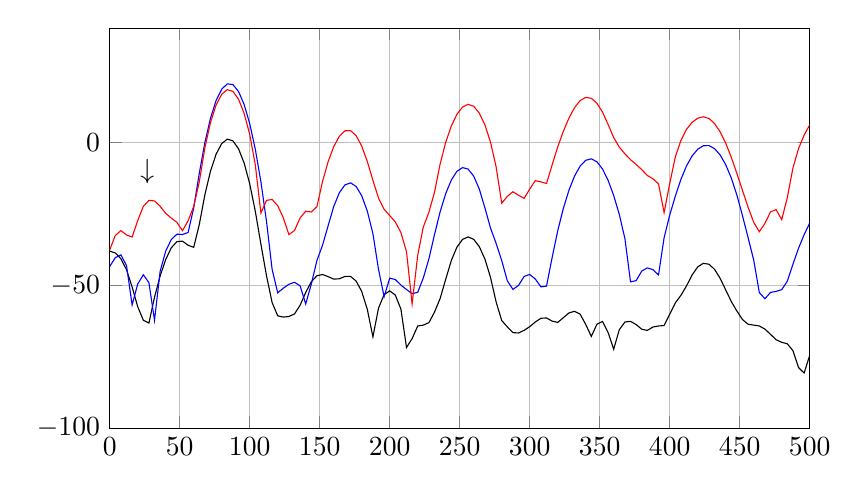
\begin{tikzpicture}

\begin{axis}[%
width=3.5in,
height=2in,
at={(1.011in,0.642in)},
scale only axis,
xmin=0,
xmax=500,
xmajorgrids,
ymin=-100,
ymax=40,
ymajorgrids,
axis background/.style={fill=white}
]
\addplot [color=black,solid,forget plot]
  table[row sep=crcr]{%
0	-38.0274555726395\\
4	-38.651510611096\\
8	-40.6835763316498\\
12	-44.5233654500604\\
16	-50.5494858102553\\
20	-57.4700123218112\\
24	-62.1915564815908\\
28	-63.2015757055571\\
32	-54.1218863275567\\
36	-46.7487138690542\\
40	-40.9467290971577\\
44	-36.8449273638547\\
48	-34.6845233881249\\
52	-34.5213223402229\\
56	-35.9724280699072\\
60	-36.6772737174246\\
64	-28.6674271528343\\
68	-18.217194558207\\
72	-9.98898832926547\\
76	-4.07106545272432\\
80	-0.368076395792921\\
84	1.17496969933739\\
88	0.57648701822052\\
92	-2.18100275090489\\
96	-7.15399795021485\\
100	-14.4358816984991\\
104	-24.0845508427543\\
108	-35.5872503008305\\
112	-46.6533889283533\\
116	-56.0159710677634\\
120	-60.6550679437631\\
124	-61.1055884826112\\
128	-60.8914381351916\\
132	-59.9969714581076\\
136	-56.961622761581\\
140	-52.4685344957774\\
144	-48.7441524039528\\
148	-46.6356131655313\\
152	-46.1873930059594\\
156	-46.9294906633472\\
160	-47.8119777204146\\
164	-47.690591819093\\
168	-46.8825826837565\\
172	-46.8467537669325\\
176	-48.4812066997519\\
180	-52.1230163540569\\
184	-58.4130128830048\\
188	-68.0277111120983\\
192	-57.9616775131286\\
196	-53.2450080795827\\
200	-51.9276258767901\\
204	-53.4022926298902\\
208	-58.2944443907168\\
212	-71.7513621041689\\
216	-68.6214018310109\\
220	-64.226375355091\\
224	-63.9068612395794\\
228	-63.038755922395\\
232	-59.337501072354\\
236	-54.6065716671905\\
240	-47.8602213041462\\
244	-41.3008993018352\\
248	-36.6230946669406\\
252	-33.916708414835\\
256	-33.0403505324789\\
260	-33.8949126465404\\
264	-36.4534736831729\\
268	-40.8004216113336\\
272	-47.2091926461091\\
276	-55.8003263410948\\
280	-62.3018911750458\\
284	-64.5183699939363\\
288	-66.5260434820862\\
292	-66.6689534979108\\
296	-65.7399646598643\\
300	-64.4553768445702\\
304	-62.8090792179468\\
308	-61.5184170600924\\
312	-61.409428082822\\
316	-62.5089007537359\\
320	-62.9672255922981\\
324	-61.3151784822181\\
328	-59.6465779354599\\
332	-59.0805500683714\\
336	-60.0520220813974\\
340	-63.6684212256777\\
344	-67.8650569029938\\
348	-63.6145972565869\\
352	-62.6113255319151\\
356	-66.5332569352241\\
360	-72.3413883143577\\
364	-65.4869930777221\\
368	-62.8241742905383\\
372	-62.603640786007\\
376	-63.7009271841737\\
380	-65.3439536321743\\
384	-65.7621155427093\\
388	-64.5711051161714\\
392	-64.2122257683203\\
396	-64.0517515513743\\
400	-60.0481779467032\\
404	-56.139558664776\\
408	-53.481882026631\\
412	-50.1915366081094\\
416	-46.3459535148488\\
420	-43.5300566698413\\
424	-42.2792601277519\\
428	-42.5902476011542\\
432	-44.3717448113664\\
436	-47.5066147122243\\
440	-51.6149698430641\\
444	-55.6547865192127\\
448	-59.0071528291873\\
452	-61.9659362438547\\
456	-63.6229866445944\\
460	-63.9089786117354\\
464	-64.2017429080807\\
468	-65.312220967396\\
472	-67.1370698885016\\
476	-69.0213987218657\\
480	-69.9237881641573\\
484	-70.4430906235884\\
488	-72.8338583973933\\
492	-78.7585037642878\\
496	-80.6933197777078\\
500	-74.4632736943004\\
504	-70.137881697582\\
508	-67.6291851874067\\
512	-66.0380968106471\\
516	-64.1685585058744\\
520	-61.5993519551501\\
524	-59.1616558907\\
528	-57.8580636404769\\
532	-58.2478511949161\\
536	-60.8975793145943\\
540	-67.3107579802983\\
544	-77.5102035170677\\
548	-69.4470538260138\\
552	-65.9477415578579\\
556	-63.3861497092942\\
560	-62.189659854753\\
564	-63.05419065671\\
568	-66.4441680633171\\
572	-71.7919763266831\\
576	-74.4413599521287\\
580	-69.1442425973303\\
584	-62.2324157968637\\
588	-57.8117479177173\\
592	-55.3099854451853\\
596	-54.3061345310736\\
600	-54.492214457945\\
604	-55.5345697121743\\
608	-57.2129007425673\\
612	-59.611069848711\\
616	-62.8486192253795\\
620	-65.4442229717601\\
624	-64.1611597343069\\
628	-62.0572343559091\\
632	-61.2131948743062\\
636	-61.3723290567409\\
640	-62.2728141000599\\
644	-64.5408708705395\\
648	-69.3891540360687\\
652	-75.2600777076656\\
656	-77.2967418745545\\
660	-73.0885715624367\\
664	-64.2566587198973\\
668	-58.983919626915\\
672	-55.612019762241\\
676	-53.4304509190285\\
680	-52.3352980785938\\
684	-52.3131380776613\\
688	-52.9910755577907\\
692	-53.45994409383\\
696	-53.2232486924585\\
700	-53.0632593649822\\
704	-53.8482035684902\\
708	-56.0268159322002\\
712	-59.9002075018575\\
716	-65.5845051587413\\
720	-71.73880705115\\
724	-73.7305076346682\\
728	-71.7899617026951\\
732	-70.3465628181033\\
736	-69.9235488115039\\
740	-68.3500493510006\\
744	-65.4858938304006\\
748	-63.0990225195289\\
752	-61.6067833505333\\
756	-60.7561831213815\\
760	-59.6135611298982\\
764	-57.6993845370081\\
768	-56.0149856400505\\
772	-55.2990461486835\\
776	-55.6143224667382\\
780	-56.5230422973192\\
784	-56.7655518398845\\
788	-55.5497234204546\\
792	-54.2867612932208\\
796	-54.2374383147607\\
800	-55.9235668640229\\
804	-60.0211339650426\\
808	-69.392783536282\\
812	-68.2774347254717\\
816	-61.8711437691045\\
820	-59.8143591770845\\
824	-59.7085752657574\\
828	-60.5332201184619\\
832	-61.5482356427328\\
836	-62.7970677436238\\
840	-65.4356004016079\\
844	-73.3304802160536\\
848	-75.4632393930567\\
852	-67.2311754838402\\
856	-66.0451411683259\\
860	-67.5172965871505\\
864	-69.9982709325867\\
868	-71.0949444174672\\
872	-69.3751311114515\\
876	-68.1962674719523\\
880	-69.2820852140989\\
884	-69.9732295369882\\
888	-64.942848732347\\
892	-61.8114173339963\\
896	-61.7280359252529\\
900	-63.330397873676\\
904	-62.7084147725373\\
908	-61.1993606250884\\
912	-61.8865060894373\\
916	-66.1352503333639\\
920	-71.3961049590045\\
924	-63.4914316028642\\
928	-59.4893787582751\\
932	-57.6040297101834\\
936	-56.6507025754931\\
940	-56.1513063888604\\
944	-55.9726774405508\\
948	-56.1822319007531\\
952	-56.9715190553563\\
956	-58.5286135286604\\
960	-60.539669180608\\
964	-60.8979436594205\\
968	-59.4488566654333\\
972	-59.2029779860874\\
976	-60.8103860406542\\
980	-63.0984661606324\\
984	-66.8749639868725\\
988	-93.7770054278073\\
992	-63.5962092707241\\
996	-56.9039233691331\\
1000	-54.3012723414932\\
1004	-54.4454133412867\\
1008	-54.5784275824147\\
1012	-51.667584559036\\
1016	-48.9877320534642\\
1020	-47.5648322999433\\
1024	-46.9221756905675\\
1028	-46.6555116232875\\
1032	-46.5808228735464\\
1036	-46.6165858788683\\
1040	-46.7967088368173\\
1044	-47.3352242709638\\
1048	-48.4821045128991\\
1052	-50.2155259347497\\
1056	-52.5980515509452\\
1060	-57.1104362803267\\
1064	-69.2495896880599\\
1068	-70.4230298867048\\
1072	-77.0230701341889\\
1076	-65.6015113082796\\
1080	-58.7495367424867\\
1084	-56.1122384637935\\
1088	-54.6197489660603\\
1092	-53.4888725709275\\
1096	-52.1717658716985\\
1100	-50.4737979360558\\
1104	-48.754576439484\\
1108	-47.2788849377688\\
1112	-46.1278464145447\\
1116	-45.3452827208905\\
1120	-44.9415830862347\\
1124	-44.9059304560528\\
1128	-45.3295453620217\\
1132	-46.3400247415685\\
1136	-47.5972346056926\\
1140	-48.5408768140981\\
1144	-49.9760417805454\\
1148	-52.2960959057686\\
1152	-53.7452214258224\\
1156	-56.9284559619679\\
1160	-62.1983626837934\\
1164	-55.2331246047165\\
1168	-53.6350338568012\\
1172	-54.0785790865471\\
1176	-51.5298711815517\\
1180	-48.2225763742529\\
1184	-45.968866340988\\
1188	-44.7000080450072\\
1192	-44.1590281645503\\
1196	-44.0720625799004\\
1200	-44.2606607154458\\
1204	-44.6643917564106\\
1208	-45.28717366384\\
1212	-46.2578905381685\\
1216	-47.8825121972825\\
1220	-50.1872290624615\\
1224	-52.2964381234626\\
1228	-54.5654138037768\\
1232	-59.4211047759978\\
1236	-59.7320146716102\\
1240	-56.4741031173961\\
1244	-56.104168202275\\
1248	-54.9399498967894\\
1252	-53.4808338164693\\
1256	-53.1969443747193\\
1260	-52.6544665614655\\
1264	-50.8539727315007\\
1268	-48.4204726450024\\
1272	-46.0931974334673\\
1276	-44.2850464014188\\
1280	-43.0415156918079\\
1284	-42.2575078748721\\
1288	-41.8029142436049\\
1292	-41.5748918323117\\
1296	-41.5936590981438\\
1300	-41.9733829068176\\
1304	-42.6435682298194\\
1308	-43.3643245771858\\
1312	-44.5384194363157\\
1316	-47.1375399964247\\
1320	-50.5127252359422\\
1324	-51.4510642997632\\
1328	-54.1626759133009\\
1332	-70.2821383422248\\
1336	-54.9774005959377\\
1340	-51.1457069381935\\
1344	-50.4261659512397\\
1348	-49.8120064355495\\
1352	-49.213892937487\\
1356	-49.0096979174814\\
1360	-48.7202561322586\\
1364	-48.4236043306856\\
1368	-48.609851464664\\
1372	-49.3553403090318\\
1376	-50.4293674656735\\
1380	-51.7709965537079\\
1384	-53.6619618506605\\
1388	-55.3092818999759\\
1392	-54.1670383845034\\
1396	-52.8578967469143\\
1400	-54.0896201647106\\
1404	-56.9737654788055\\
1408	-55.3488048838864\\
1412	-54.3415536399013\\
1416	-57.9689298152135\\
1420	-68.5792142703289\\
1424	-59.3822448331627\\
1428	-56.7946391905853\\
1432	-57.8026494089227\\
1436	-61.3140297633209\\
1440	-65.955517703424\\
1444	-61.2993992378116\\
1448	-56.9982933089461\\
1452	-55.2327447885493\\
1456	-54.9679175852459\\
1460	-55.229544969534\\
1464	-55.4130088771088\\
1468	-55.7857526939584\\
1472	-57.1061803327872\\
1476	-59.4949454704973\\
1480	-60.9348593232694\\
1484	-61.1030610222408\\
1488	-61.1412877238631\\
1492	-58.9500503672795\\
1496	-57.2665596985633\\
1500	-58.2723082223923\\
1504	-62.7450794865743\\
1508	-72.2926587717089\\
1512	-80.2439461450564\\
1516	-66.9658424950025\\
1520	-60.4558247176021\\
1524	-57.574648651393\\
1528	-56.8023980038337\\
1532	-56.9657275917647\\
1536	-57.1277988133015\\
1540	-57.2852728653788\\
1544	-58.0335406400863\\
1548	-59.6972629334685\\
1552	-61.5180105753411\\
1556	-60.9211644011517\\
1560	-59.0392843514323\\
1564	-58.5932470768602\\
1568	-60.6147300881071\\
1572	-65.9827313731715\\
1576	-64.6362009504159\\
1580	-59.9379942535435\\
1584	-59.1633107101623\\
1588	-61.8248112598995\\
1592	-65.2636451481702\\
1596	-63.2562057736505\\
1600	-62.5042611713492\\
1604	-63.4779509561759\\
1608	-63.4058068974005\\
1612	-62.5610840181426\\
1616	-62.1216097501841\\
1620	-61.568411800801\\
1624	-60.7144014544403\\
1628	-60.063203569066\\
1632	-59.9522044033908\\
1636	-60.3876457018285\\
1640	-60.7187939394052\\
1644	-59.9499618398129\\
1648	-58.7496154157564\\
1652	-58.4033836848094\\
1656	-59.0754005891751\\
1660	-59.8077352733209\\
1664	-60.4526711560627\\
1668	-63.4717811596879\\
1672	-72.7300489419727\\
1676	-61.7738788739844\\
1680	-56.9936865219213\\
1684	-55.828525334699\\
1688	-56.7905077495865\\
1692	-58.8955730399589\\
1696	-60.5812521887272\\
1700	-60.1388152933452\\
1704	-58.1014000435503\\
1708	-56.1911550183637\\
1712	-55.145936792147\\
1716	-54.9462014924982\\
1720	-55.4988695337568\\
1724	-56.7290381992657\\
1728	-57.9482795885427\\
1732	-57.9870796943658\\
1736	-57.7063994459606\\
1740	-58.8453749233269\\
1744	-62.7831354631206\\
1748	-71.2585815524349\\
1752	-67.9301050995896\\
1756	-66.5005526093112\\
1760	-73.3680443829787\\
1764	-69.767232784737\\
1768	-62.944242922702\\
1772	-60.8933010836498\\
1776	-60.1028537511172\\
1780	-59.0899460247182\\
1784	-58.6963777225884\\
1788	-59.5325195737462\\
1792	-60.7120465046566\\
1796	-60.6027956009386\\
1800	-59.2804075846378\\
1804	-58.2244518112064\\
1808	-57.8635788435529\\
1812	-57.7636153807415\\
1816	-57.7977063123455\\
1820	-58.7054842328834\\
1824	-61.6906460263396\\
1828	-67.0047562847722\\
1832	-64.9368597592961\\
1836	-62.155324079149\\
1840	-62.570654447902\\
1844	-65.3915861407517\\
1848	-68.0858724316826\\
1852	-67.5873083101635\\
1856	-68.1137044084679\\
1860	-74.238185959802\\
1864	-76.2752168771078\\
1868	-66.0671532072126\\
1872	-62.9907148764615\\
1876	-62.0840625017617\\
1880	-61.6615515847913\\
1884	-61.33308115305\\
1888	-61.2008491115537\\
1892	-60.8694873582207\\
1896	-60.2813707975354\\
1900	-60.0765171582144\\
1904	-60.8023568022474\\
1908	-62.9840088773219\\
1912	-67.0449633586464\\
1916	-67.7833046556872\\
1920	-64.0017440942996\\
1924	-62.9169384400472\\
1928	-65.1643620458734\\
1932	-67.9367999078171\\
1936	-64.7358194498073\\
1940	-62.9736219302299\\
1944	-63.9951322409516\\
1948	-65.6318558754709\\
1952	-63.3386825227192\\
1956	-60.8748372978022\\
1960	-60.0784015113095\\
1964	-60.5504304600666\\
1968	-61.767727995823\\
1972	-63.2661696528192\\
1976	-64.5040726637251\\
1980	-63.2487431603555\\
1984	-60.3180182421082\\
1988	-58.6296215862558\\
1992	-58.8787400921962\\
1996	-61.5520071115623\\
2000	-68.8617800939407\\
2004	-65.7515913023238\\
2008	-58.7249266616689\\
2012	-56.0676211737599\\
2016	-56.1326244518792\\
2020	-58.5866575476027\\
2024	-63.6882244785513\\
2028	-70.9484983190913\\
2032	-68.4101236106035\\
2036	-63.8815697443392\\
2040	-60.5520520450695\\
2044	-58.158550092216\\
2048	-56.5070704749861\\
2052	-55.3135084081071\\
2056	-54.4670923386552\\
2060	-54.1116952476219\\
2064	-54.2237859339789\\
2068	-54.5518536179199\\
2072	-55.3057748946875\\
2076	-57.057112408761\\
2080	-59.9154092378074\\
2084	-62.5158887016593\\
2088	-62.8253063495721\\
2092	-62.2111852647942\\
2096	-61.6340709452282\\
2100	-60.9765321713009\\
2104	-60.7870494520864\\
2108	-61.9909602359863\\
2112	-65.561122484628\\
2116	-71.1200334227455\\
2120	-68.5657530126375\\
2124	-65.5842769379401\\
2128	-65.1029632773355\\
2132	-66.4791122999571\\
2136	-69.16419153044\\
2140	-70.45506655405\\
2144	-69.192472110601\\
2148	-68.6909610175356\\
2152	-69.8781181741165\\
2156	-73.0425575301423\\
2160	-77.4864925077327\\
2164	-75.0456506082266\\
2168	-70.8791649847619\\
2172	-66.9123955292587\\
2176	-62.8373852569631\\
2180	-60.1097733655119\\
2184	-59.3088682462166\\
2188	-60.4902436203128\\
2192	-63.5296112638169\\
2196	-67.7940650482664\\
2200	-71.8372441148372\\
2204	-73.6840821837811\\
2208	-71.9459863662717\\
2212	-69.0575397620188\\
2216	-66.1594307139509\\
2220	-64.3644810730045\\
2224	-64.2012567925309\\
2228	-65.0459354534432\\
2232	-65.0201559141112\\
2236	-63.4739366796754\\
2240	-61.926674928098\\
2244	-61.4391195875663\\
2248	-62.4444576217463\\
2252	-65.4487227707562\\
2256	-73.2462069516213\\
2260	-75.1616102081732\\
2264	-64.7796549395745\\
2268	-61.3684108861175\\
2272	-61.2802598453211\\
2276	-64.6369613202028\\
2280	-68.2833399967633\\
2284	-63.0599854915843\\
2288	-60.3870921768897\\
2292	-60.0622089908533\\
2296	-60.4956739861318\\
2300	-60.0813428318324\\
2304	-58.9943692873587\\
2308	-58.3553180349909\\
2312	-58.1268790491532\\
2316	-57.558097837931\\
2320	-56.4635401430704\\
2324	-55.3927800746486\\
2328	-54.8820598081227\\
2332	-55.2659003813685\\
2336	-56.8252294501309\\
2340	-59.7737531998268\\
2344	-62.4198892783782\\
2348	-60.7836640424831\\
2352	-58.7536433009593\\
2356	-58.5041378799219\\
2360	-60.3003236628672\\
2364	-64.4775500500934\\
2368	-68.1259093511918\\
2372	-65.1868250231584\\
2376	-63.072811308629\\
2380	-62.9486276997308\\
2384	-64.7809750661403\\
2388	-68.6901614794723\\
2392	-73.6530822030932\\
2396	-80.3477143526205\\
};
\addplot [color=blue,solid,forget plot]
  table[row sep=crcr]{%
0	-43.3793333653497\\
4	-40.3104074880648\\
8	-39.3343949048748\\
12	-43.0667070952237\\
16	-56.8593344003102\\
20	-49.5377657318789\\
24	-46.2902680751464\\
28	-49.0254608073622\\
32	-62.2112941351337\\
36	-45.127232545234\\
40	-38.0056148667537\\
44	-33.9338484427806\\
48	-32.0828662152842\\
52	-32.1982917172143\\
56	-31.4821735138688\\
60	-22.8655731909516\\
64	-10.7005925377524\\
68	0.0540293971939503\\
72	8.52262495745948\\
76	14.7081334404157\\
80	18.690352112864\\
84	20.5293089668683\\
88	20.2555253944393\\
92	17.8697457806083\\
96	13.3435663070214\\
100	6.62077602287799\\
104	-2.3778171845483\\
108	-13.743045917769\\
112	-27.6075523993343\\
116	-44.3785135739019\\
120	-52.6093543529198\\
124	-50.9835650985259\\
128	-49.6127856724579\\
132	-48.9214129314788\\
136	-50.1586517401853\\
140	-56.5166402963115\\
144	-49.5426130375589\\
148	-41.2931990878615\\
152	-35.9584353041409\\
156	-29.1425295287302\\
160	-22.4167828598289\\
164	-17.5989777644926\\
168	-14.8519201225955\\
172	-14.1153107263682\\
176	-15.3676549512609\\
180	-18.6366059723657\\
184	-24.0218569707202\\
188	-31.8801018843686\\
192	-44.4019115353234\\
196	-53.9604355397262\\
200	-47.4716612502541\\
204	-47.9622560166994\\
208	-49.9081820064492\\
212	-51.4481420244574\\
216	-52.8987844002606\\
220	-52.4268309247318\\
224	-47.4032528078041\\
228	-40.678373708595\\
232	-32.213613011654\\
236	-24.2783775098433\\
240	-17.8892964036151\\
244	-13.1445435045851\\
248	-10.0847345912792\\
252	-8.7757067402525\\
256	-9.30067268067702\\
260	-11.7700418769846\\
264	-16.3152552441688\\
268	-22.8676079973536\\
272	-29.9371903897859\\
276	-35.2952556496479\\
280	-41.3013989899267\\
284	-48.391148516396\\
288	-51.4051281166252\\
292	-50.0047091263776\\
296	-46.8873838865238\\
300	-46.1725893016671\\
304	-47.7839415451967\\
308	-50.5179705611921\\
312	-50.2662163599615\\
316	-40.2847079657027\\
320	-30.9121020781833\\
324	-23.0969634916931\\
328	-16.7335730289225\\
332	-11.7722112422993\\
336	-8.2498182628668\\
340	-6.22050884783891\\
344	-5.71681144250457\\
348	-6.74257597357052\\
352	-9.27142079184058\\
356	-13.2434536005644\\
360	-18.5661698976219\\
364	-25.1883206299739\\
368	-33.6507199782958\\
372	-48.7684801760672\\
376	-48.3533606009608\\
380	-45.0055042272334\\
384	-43.8831264111822\\
388	-44.505011241597\\
392	-46.3587900589017\\
396	-33.2871522072958\\
400	-25.4133197391412\\
404	-18.7857089099903\\
408	-12.9041000763319\\
412	-8.19030875825299\\
416	-4.6927309754909\\
420	-2.35154989111149\\
424	-1.14333965070649\\
428	-1.06741014323903\\
432	-2.12932068882579\\
436	-4.34708559916792\\
440	-7.76243282597698\\
444	-12.4413729451656\\
448	-18.4423525233541\\
452	-25.6466737740787\\
456	-33.3316753603064\\
460	-41.1529404152644\\
464	-52.4985526909053\\
468	-54.6808743870508\\
472	-52.4585222168964\\
476	-52.1172280014828\\
480	-51.4949103360752\\
484	-48.5209498649854\\
488	-42.608642685797\\
492	-37.0273393090303\\
496	-32.2659757001395\\
500	-28.1587681429875\\
504	-24.7034795885027\\
508	-21.9590070953369\\
512	-19.9592761228645\\
516	-18.7019187405112\\
520	-18.160621090324\\
524	-18.3088621145862\\
528	-19.1650629425827\\
532	-20.8597405986809\\
536	-23.7099324155317\\
540	-28.3497794729038\\
544	-36.055274181805\\
548	-44.0523877096354\\
552	-43.6738325735485\\
556	-47.6415397601959\\
560	-51.674159829837\\
564	-45.7727669400794\\
568	-41.2630229263906\\
572	-39.210442353446\\
576	-37.4791129177693\\
580	-34.642868441494\\
584	-31.6496130672136\\
588	-29.2056856928665\\
592	-27.3182612539967\\
596	-25.9793686476967\\
600	-25.24402199331\\
604	-25.1292855250358\\
608	-25.6143395160166\\
612	-26.6907790201062\\
616	-28.3990307775905\\
620	-30.8087213546125\\
624	-33.8371086255296\\
628	-37.1282646437246\\
632	-39.9216767415908\\
636	-41.9198972231072\\
640	-45.3561965057236\\
644	-43.401610440659\\
648	-41.7465223669117\\
652	-40.1135304210367\\
656	-37.481234481949\\
660	-35.0013974218215\\
664	-32.1736879074796\\
668	-30.0041898906898\\
672	-28.7948191153829\\
676	-28.4494523349263\\
680	-28.9550431951451\\
684	-30.3782451679085\\
688	-32.8276887878465\\
692	-36.3869180643404\\
696	-40.6469317934961\\
700	-43.8460476335852\\
704	-45.8024861600988\\
708	-49.0913005855115\\
712	-56.0593884504153\\
716	-65.4782241106255\\
720	-63.8454294569943\\
724	-69.4073591721873\\
728	-69.4886651960317\\
732	-57.4286855134977\\
736	-49.8592902473402\\
740	-46.8923724311517\\
744	-47.2924831138272\\
748	-46.8889458579998\\
752	-41.5526601133183\\
756	-37.2964656779155\\
760	-34.4817387776398\\
764	-32.4297100124371\\
768	-30.8237288533105\\
772	-29.6993943474942\\
776	-29.2562958295557\\
780	-29.7003678108406\\
784	-31.1343798576777\\
788	-33.2594857375315\\
792	-35.1162238438634\\
796	-36.484312767024\\
800	-37.9389996580759\\
804	-39.6619894728682\\
808	-44.7838133302906\\
812	-52.6493762076393\\
816	-39.7402734881509\\
820	-35.9929503103073\\
824	-34.0515931270673\\
828	-32.3738546597342\\
832	-29.6853133422157\\
836	-26.1105753686617\\
840	-22.905658221372\\
844	-20.4428317097388\\
848	-18.6933715169628\\
852	-17.5828632654678\\
856	-17.0425879448727\\
860	-17.0379082595022\\
864	-17.5920438019755\\
868	-18.8202006919413\\
872	-20.985758149233\\
876	-24.5372792473756\\
880	-30.1422283303192\\
884	-38.4941739586769\\
888	-39.1675959820217\\
892	-35.9770636412854\\
896	-35.9837951938162\\
900	-37.6507840707315\\
904	-36.4546285898191\\
908	-31.8307518074081\\
912	-29.5673028948434\\
916	-26.7267207339616\\
920	-22.1641188150572\\
924	-18.8038016897896\\
928	-16.8931535702649\\
932	-15.9616065153281\\
936	-15.6074692762265\\
940	-15.7067777165691\\
944	-16.4405199649414\\
948	-17.995627202956\\
952	-20.236624287773\\
956	-22.5528204447799\\
960	-24.3467409555328\\
964	-25.8417998422323\\
968	-28.3030980080263\\
972	-30.7982834094398\\
976	-29.1492915118198\\
980	-30.7322391576134\\
984	-46.7786617255289\\
988	-34.3185154076249\\
992	-31.4994064141801\\
996	-29.471947845708\\
1000	-26.2020277397225\\
1004	-24.1162608878236\\
1008	-22.7774954804273\\
1012	-21.6124033413948\\
1016	-20.4382114401136\\
1020	-19.6318822809056\\
1024	-19.5111549108456\\
1028	-20.0662846616352\\
1032	-21.1821291935389\\
1036	-22.7998722631442\\
1040	-24.969897238222\\
1044	-27.7791222122827\\
1048	-31.0237547970521\\
1052	-33.9795365548093\\
1056	-35.5876768800113\\
1060	-36.0104428196091\\
1064	-38.5366062876057\\
1068	-46.6676251410762\\
1072	-41.6840477305458\\
1076	-37.940817026508\\
1080	-35.5455435648283\\
1084	-33.1089360149878\\
1088	-31.4112712147719\\
1092	-29.7619984358559\\
1096	-28.2431184154168\\
1100	-27.4767973175203\\
1104	-27.5369182647338\\
1108	-28.1977854758007\\
1112	-29.2081675384176\\
1116	-30.3518829691763\\
1120	-31.4766566046055\\
1124	-32.5504742869138\\
1128	-33.9429754849402\\
1132	-36.3337696764089\\
1136	-37.7598431027261\\
1140	-35.6332110889659\\
1144	-35.1812858974422\\
1148	-38.7123757190464\\
1152	-49.9803034826085\\
1156	-54.9234350249867\\
1160	-46.6693080385205\\
1164	-39.0938078790283\\
1168	-35.5478265256394\\
1172	-34.7837490630541\\
1176	-36.0469638739989\\
1180	-39.4433693162365\\
1184	-45.3819185903671\\
1188	-46.1932906690418\\
1192	-43.8421185270868\\
1196	-44.7188637291212\\
1200	-47.7256844593601\\
1204	-50.2039792052004\\
1208	-50.3599426535444\\
1212	-45.3363154883364\\
1216	-41.1751306692493\\
1220	-39.7800768530546\\
1224	-40.3817272041452\\
1228	-41.2514162330106\\
1232	-39.7015757304511\\
1236	-36.4174054035097\\
1240	-34.3396832873636\\
1244	-34.4971016331685\\
1248	-37.5279976614601\\
1252	-47.1007051847878\\
1256	-44.1438351026218\\
1260	-35.0266469531028\\
1264	-30.7174847282733\\
1268	-28.382451052974\\
1272	-27.3726294512991\\
1276	-27.5028960486777\\
1280	-28.6818613763131\\
1284	-30.7200838059278\\
1288	-33.2735019616364\\
1292	-34.6129820901356\\
1296	-32.2424149238019\\
1300	-29.1615018612742\\
1304	-27.9483187275349\\
1308	-29.0239222059131\\
1312	-31.673658060613\\
1316	-33.8859026741715\\
1320	-34.534098933047\\
1324	-33.248888652925\\
1328	-32.3473560820903\\
1332	-32.5171939460971\\
1336	-32.1461269545508\\
1340	-32.4015895031074\\
1344	-35.7334967275228\\
1348	-46.6960270281217\\
1352	-45.6698458965438\\
1356	-40.5171558524363\\
1360	-39.7953987048741\\
1364	-39.2664310604665\\
1368	-38.2786483959244\\
1372	-37.4362082190928\\
1376	-36.7642724702497\\
1380	-35.6939420086857\\
1384	-34.2415204792634\\
1388	-33.3460212046781\\
1392	-33.6907264000125\\
1396	-34.3413017470434\\
1400	-33.3600559652187\\
1404	-32.6834024159628\\
1408	-34.7017083496984\\
1412	-41.320721371547\\
1416	-41.1809979065804\\
1420	-36.5447164059511\\
1424	-36.0924184916698\\
1428	-37.205354804001\\
1432	-36.5692406595394\\
1436	-34.814231261706\\
1440	-33.8527291854732\\
1444	-33.7335796392769\\
1448	-34.2362643966751\\
1452	-35.430733564662\\
1456	-37.6158553424706\\
1460	-41.2635634767616\\
1464	-46.4199174735935\\
1468	-51.3029258991769\\
1472	-68.9312431838497\\
1476	-45.8015124690331\\
1480	-39.9528142701708\\
1484	-38.4486268329344\\
1488	-39.7017979204687\\
1492	-41.7066702949979\\
1496	-42.1311363950127\\
1500	-43.6902832679481\\
1504	-50.0699595158331\\
1508	-62.4433698223954\\
1512	-51.6445363307665\\
1516	-52.8820156711677\\
1520	-52.1275507359403\\
1524	-46.8584583255144\\
1528	-44.237431584167\\
1532	-43.4797840278924\\
1536	-43.5448881706329\\
1540	-43.1731442909405\\
1544	-42.1305321135139\\
1548	-41.3993419142891\\
1552	-41.1384776417632\\
1556	-40.6134518930494\\
1560	-39.7421769424453\\
1564	-39.3916401712373\\
1568	-40.4221677240796\\
1572	-43.5448681247163\\
1576	-49.1945211753609\\
1580	-54.2071665173561\\
1584	-54.5113885334975\\
1588	-51.9293909081478\\
1592	-47.2470171152513\\
1596	-43.5862229977316\\
1600	-41.297946584517\\
1604	-40.1858887865353\\
1608	-39.95996342474\\
1612	-40.0364617344045\\
1616	-39.714680846606\\
1620	-39.1209561234104\\
1624	-39.1440025496384\\
1628	-40.1337322567669\\
1632	-41.2415195641443\\
1636	-41.1387863128901\\
1640	-40.1611186863529\\
1644	-39.1780451476729\\
1648	-38.5091950566943\\
1652	-38.4406782068308\\
1656	-39.275700011611\\
1660	-40.7517937177982\\
1664	-42.0610057862875\\
1668	-43.311806307408\\
1672	-45.4882902731927\\
1676	-49.119908148701\\
1680	-49.2485405243858\\
1684	-45.0966284990019\\
1688	-43.0777913450606\\
1692	-43.6734911746418\\
1696	-47.1047204851452\\
1700	-53.5413462113875\\
1704	-53.90996374643\\
1708	-49.3085158025794\\
1712	-45.5248319038693\\
1716	-42.7109542475869\\
1720	-40.9650492425755\\
1724	-40.1295532834476\\
1728	-39.7548282076696\\
1732	-39.1359386025259\\
1736	-38.0870545350802\\
1740	-37.1948851426132\\
1744	-37.1196718975624\\
1748	-38.3813266032709\\
1752	-41.4782021543896\\
1756	-47.123814870517\\
1760	-55.1853923056855\\
1764	-54.2215113840618\\
1768	-50.4050982857326\\
1772	-47.3364536355384\\
1776	-45.7680261531044\\
1780	-46.0356660913151\\
1784	-47.9067816018557\\
1788	-50.2435269645061\\
1792	-50.4065642764461\\
1796	-46.9769020780493\\
1800	-43.155202907089\\
1804	-40.6900930154162\\
1808	-39.6237203192433\\
1812	-39.7211431391672\\
1816	-40.7315048723526\\
1820	-42.2720922302826\\
1824	-43.6420245404219\\
1828	-44.2131694497876\\
1832	-44.1107296394363\\
1836	-43.875146238833\\
1840	-44.0366122252439\\
1844	-44.8889255172476\\
1848	-46.3904590030166\\
1852	-48.0466717988562\\
1856	-48.5895001521002\\
1860	-47.7914939592902\\
1864	-47.1289272146687\\
1868	-46.9773444669621\\
1872	-46.6696071399298\\
1876	-45.7888976914351\\
1880	-44.6925371750158\\
1884	-43.8216065694593\\
1888	-43.5980200899648\\
1892	-44.4114163646312\\
1896	-45.2886020873062\\
1900	-43.6061291379996\\
1904	-41.157342804694\\
1908	-39.9966191518026\\
1912	-40.4466147849386\\
1916	-42.7129116309631\\
1920	-47.5293646467304\\
1924	-56.6184446173826\\
1928	-53.6598405560101\\
1932	-49.8274396579189\\
1936	-49.3415981992721\\
1940	-51.0332633223516\\
1944	-54.6947214574421\\
1948	-57.7392492830673\\
1952	-53.5253517120251\\
1956	-48.7329500637986\\
1960	-45.4162462017859\\
1964	-43.6506575298472\\
1968	-43.327160914285\\
1972	-43.7706696798571\\
1976	-43.8853771843637\\
1980	-43.5614552983897\\
1984	-43.526917040746\\
1988	-44.1120114354727\\
1992	-45.2625175792014\\
1996	-46.9581344859802\\
2000	-49.6073316323388\\
2004	-54.1684050401325\\
2008	-58.2132145770142\\
2012	-53.7604682420787\\
2016	-50.8723798262948\\
2020	-50.7589080423325\\
2024	-53.0326241497676\\
2028	-51.7396910575994\\
2032	-47.1184440768288\\
2036	-44.7801648135784\\
2040	-44.5777417285831\\
2044	-45.6586220894999\\
2048	-46.3349222445907\\
2052	-45.2068202838084\\
2056	-43.4003060175184\\
2060	-42.0567538666727\\
2064	-41.3632341323322\\
2068	-41.0195900150956\\
2072	-40.4360492738271\\
2076	-39.4236786417379\\
2080	-38.6719029817232\\
2084	-39.0553378891916\\
2088	-41.209560381275\\
2092	-45.8806134501815\\
2096	-53.5837519363167\\
2100	-50.6630039280609\\
2104	-46.8784803447698\\
2108	-45.6960584336912\\
2112	-45.9601342708314\\
2116	-46.8670445976655\\
2120	-47.4656990272437\\
2124	-47.0041569099676\\
2128	-45.6866653851499\\
2132	-44.248062741998\\
2136	-43.1773430089917\\
2140	-42.596560284208\\
2144	-42.6275967673126\\
2148	-43.693841016409\\
2152	-46.1423625647962\\
2156	-48.848150034963\\
2160	-49.0181783675961\\
2164	-48.0800192847049\\
2168	-47.7105605957354\\
2172	-48.3400959159663\\
2176	-50.34866692126\\
2180	-53.6322880121244\\
2184	-57.6181642015383\\
2188	-59.2131811944603\\
2192	-55.1233607608916\\
2196	-51.8008863031934\\
2200	-50.2517953478432\\
2204	-50.6991760092347\\
2208	-53.9398806862808\\
2212	-60.246927875092\\
2216	-55.1473176435103\\
2220	-49.7153135327897\\
2224	-46.7268057565256\\
2228	-45.2295751193025\\
2232	-44.5961797061741\\
2236	-44.3163575914134\\
2240	-44.3210829268774\\
2244	-45.0595652735571\\
2248	-47.2871249159291\\
2252	-52.0928656657296\\
2256	-55.8043544306014\\
2260	-50.2282721705792\\
2264	-46.5061991352952\\
2268	-44.5032051222647\\
2272	-43.8224298256469\\
2276	-44.3303209452262\\
2280	-45.9831161075589\\
2284	-49.4975152715889\\
2288	-58.5146722336647\\
2292	-56.2130727028928\\
2296	-50.0594630122668\\
2300	-48.7154885637919\\
2304	-49.4825879471138\\
2308	-51.7902352823369\\
2312	-54.5120462088715\\
2316	-53.2385832328784\\
2320	-52.3843925330739\\
2324	-52.7279119803419\\
2328	-49.1875255968379\\
2332	-45.8908932845971\\
2336	-45.2667140005565\\
2340	-47.8068125848763\\
2344	-56.7561241299407\\
2348	-56.1044062185524\\
2352	-48.0679669994204\\
2356	-45.4408746065714\\
2360	-45.1877366025854\\
2364	-47.0195449765416\\
2368	-51.6385522380725\\
2372	-54.876903196434\\
2376	-48.5819614646499\\
2380	-45.3543873558628\\
2384	-44.9442627016261\\
2388	-47.1361596275073\\
2392	-52.9160957208032\\
2396	-73.6690631663724\\
};
\addplot [color=red,solid,forget plot]
  table[row sep=crcr]{%
0	-37.593202458105\\
4	-32.5387620443458\\
8	-30.8122841430479\\
12	-32.3599186192166\\
16	-33.0814041560757\\
20	-27.3382090481522\\
24	-22.3550263121014\\
28	-20.2431715022246\\
32	-20.4478651256333\\
36	-22.2909561360892\\
40	-24.7778068037207\\
44	-26.4864644904208\\
48	-27.9352355388885\\
52	-30.8434918572424\\
56	-27.3904054365501\\
60	-22.3669535015182\\
64	-13.7119724899118\\
68	-1.82104793749142\\
72	6.99979737099748\\
76	13.1271643908763\\
80	16.9083414163075\\
84	18.4847148598002\\
88	17.9066797109304\\
92	15.1710945949398\\
96	10.215897639397\\
100	2.83532884438976\\
104	-7.80916972141651\\
108	-24.6797794214996\\
112	-20.2659761298403\\
116	-19.9063066044904\\
120	-22.133287492316\\
124	-26.3265168445164\\
128	-32.2431142676205\\
132	-30.7882390969197\\
136	-26.3977287201758\\
140	-24.0529377707577\\
144	-24.3126147792817\\
148	-22.4435311972716\\
152	-13.6775856756861\\
156	-6.72906827540472\\
160	-1.47445796756258\\
164	2.17925153517975\\
168	4.09145142698227\\
172	4.17469841481913\\
176	2.39127573909082\\
180	-1.25556885865565\\
184	-6.64881927350287\\
188	-13.2481389231124\\
192	-19.435261172533\\
196	-23.3631549365996\\
200	-25.5575118824393\\
204	-27.8130911659649\\
208	-31.5556407533074\\
212	-38.2043570244905\\
216	-56.5029923341118\\
220	-39.4698467250608\\
224	-29.5557758777701\\
228	-24.4056665338882\\
232	-17.3763869501723\\
236	-7.55094049522068\\
240	0.0822412084247637\\
244	5.7671305083178\\
248	9.86282489805806\\
252	12.4150719676784\\
256	13.370613665883\\
260	12.6774662093547\\
264	10.2935007047063\\
268	6.15806156579304\\
272	0.100392640540774\\
276	-8.54614956783542\\
280	-21.2252347760262\\
284	-18.8490519800895\\
288	-17.2478940671731\\
292	-18.4380372340826\\
296	-19.5657262054174\\
300	-16.2979988357667\\
304	-13.3408820835405\\
308	-13.7686540877533\\
312	-14.3610081973573\\
316	-7.86797480242334\\
320	-1.55123351110673\\
324	3.89995840052385\\
328	8.51889582152401\\
332	12.1983993481039\\
336	14.6741139612462\\
340	15.785572451455\\
344	15.4828825362641\\
348	13.7546750739755\\
352	10.6245372070125\\
356	6.29832705901459\\
360	1.70938959509664\\
364	-1.6207205462543\\
368	-3.96978466811951\\
372	-6.00729963670208\\
376	-7.68528228475012\\
380	-9.48584559726435\\
384	-11.5326372146752\\
388	-12.6884761260448\\
392	-14.4730230240182\\
396	-24.5104105868142\\
400	-14.3802508490155\\
404	-5.04724660040584\\
408	0.727036187689978\\
412	4.60596461549798\\
416	7.05765813635985\\
420	8.51057908707\\
424	9.00932393736888\\
428	8.41538994515072\\
432	6.66223937899442\\
436	3.76055778280686\\
440	-0.233145035856987\\
444	-5.18790093729145\\
448	-10.8440227372476\\
452	-16.8180910580305\\
456	-22.6684035723433\\
460	-27.9479977294683\\
464	-31.2352395298811\\
468	-28.3093503814691\\
472	-24.2672237645743\\
476	-23.4792368517034\\
480	-26.9951694417109\\
484	-19.2790146778995\\
488	-8.95438146545842\\
492	-2.14457706833809\\
496	2.60712963334266\\
500	6.14522059636192\\
504	8.97305350710479\\
508	11.1796778493197\\
512	12.655048171575\\
516	13.3079584911332\\
520	13.0773828339101\\
524	11.909036688435\\
528	9.77739472278366\\
532	6.7281920759796\\
536	2.90414973740291\\
540	-1.5332869498723\\
544	-6.60737200197449\\
548	-12.7519788182467\\
552	-20.3264594817459\\
556	-22.6311149384314\\
560	-19.2381868589412\\
564	-20.7713649901769\\
568	-34.467294223206\\
572	-15.9573307506509\\
576	-11.0823735694285\\
580	-8.61703351001005\\
584	-6.95294268190114\\
588	-5.70203523197833\\
592	-4.78289079552993\\
596	-4.16394754642475\\
600	-3.78560801418243\\
604	-3.58166394004822\\
608	-3.55990938003204\\
612	-3.84204771778599\\
616	-4.69184407367303\\
620	-6.62131605958592\\
624	-10.2038482590334\\
628	-14.753819870162\\
632	-17.6490825816842\\
636	-16.2967055247829\\
640	-21.1973891158265\\
644	-14.9276850014572\\
648	-8.91882424266648\\
652	-8.0884944442303\\
656	-4.90464170519531\\
660	-0.284046812084207\\
664	3.44309859470965\\
668	6.21952057614182\\
672	8.02395133045615\\
676	8.98267904877006\\
680	9.26684626648538\\
684	8.96573484709702\\
688	8.08410578123186\\
692	6.61822757351692\\
696	4.62659325606842\\
700	2.28135230304298\\
704	-0.165881650625083\\
708	-2.67454884736289\\
712	-5.37843813515203\\
716	-8.853769377101\\
720	-14.7844131061547\\
724	-16.585192329122\\
728	-14.3872327089371\\
732	-14.9137031892981\\
736	-18.561763482303\\
740	-9.77303646390669\\
744	-4.74484893910102\\
748	-2.2710170619697\\
752	-0.244518409926444\\
756	1.40015589648481\\
760	2.22544791388275\\
764	2.31843199462608\\
768	1.98966788179592\\
772	1.42692526694565\\
776	0.643549525101541\\
780	-0.357799726905412\\
784	-1.50490086112325\\
788	-2.88758349587211\\
792	-5.13828251195144\\
796	-8.64535439316524\\
800	-12.8159744819632\\
804	-18.012254587252\\
808	-18.236952852185\\
812	-28.9714444806249\\
816	-8.12001273325709\\
820	-2.48977632789087\\
824	-0.0635637130379939\\
828	1.71919411272239\\
832	3.7667486456229\\
836	6.02736714511627\\
840	8.0656169126697\\
844	9.50974415679797\\
848	10.3510199334089\\
852	10.7455036610759\\
856	10.7924507716151\\
860	10.4939110740861\\
864	9.83218717855051\\
868	8.83583090266306\\
872	7.53150132197859\\
876	5.89765503473516\\
880	4.11410764363244\\
884	2.4526217685597\\
888	0.519421741503794\\
892	-1.99054845299254\\
896	-6.61690720706157\\
900	-15.4895984479228\\
904	-5.34589549205052\\
908	-3.00267404236103\\
912	-0.135470281689124\\
916	3.6712062988841\\
920	6.53960704706391\\
924	9.27916622407563\\
928	11.6338217794535\\
932	13.105086260896\\
936	13.7578545591878\\
940	13.890251987486\\
944	13.7018347872785\\
948	13.1688146419644\\
952	12.1787079516313\\
956	10.6129838923048\\
960	8.24785516578569\\
964	5.42322419371403\\
968	3.50893510952147\\
972	0.372788129263664\\
976	-5.45116581891294\\
980	-2.09404272254131\\
984	-3.53243753180216\\
988	-0.27824129469636\\
992	5.08644571272517\\
996	7.49833865871785\\
1000	9.39928473763364\\
1004	11.1753731004283\\
1008	12.4516674689085\\
1012	13.3796592423684\\
1016	14.0040729706159\\
1020	14.1618712111014\\
1024	13.8112638063281\\
1028	13.0453506913286\\
1032	11.9595561401707\\
1036	10.6679046372591\\
1040	9.21777091212992\\
1044	7.24668214760669\\
1048	4.93747106918826\\
1052	4.00598994818247\\
1056	2.39938123774494\\
1060	-3.58429705208681\\
1064	-2.32501930322203\\
1068	0.146425980100884\\
1072	-2.90273344494612\\
1076	-1.06850296435607\\
1080	3.07307222163131\\
1084	5.08080736418341\\
1088	6.42230106600414\\
1092	7.24352696400452\\
1096	7.61829742472202\\
1100	7.91258772114697\\
1104	8.09026838154747\\
1108	7.85840166673046\\
1112	7.1021788379623\\
1116	5.93444912786063\\
1120	4.65248471319524\\
1124	3.33260702049799\\
1128	1.52104545965663\\
1132	0.0555870181289817\\
1136	0.415714236871292\\
1140	-0.737546851770428\\
1144	-6.10005480693188\\
1148	-3.83090930469899\\
1152	-1.04380568639799\\
1156	-4.14922919765482\\
1160	-4.75014469986619\\
1164	0.783162210582858\\
1168	2.94545809453509\\
1172	4.19802245293881\\
1176	5.51027537468856\\
1180	6.42154808887962\\
1184	6.94771016178456\\
1188	7.26534166546208\\
1192	7.21528987276464\\
1196	6.59135851913241\\
1200	5.51884605557795\\
1204	4.52056146170018\\
1208	3.66079936022354\\
1212	2.20821518634498\\
1216	1.12297679601377\\
1220	2.06392746843169\\
1224	1.38785272517869\\
1228	-3.75260826076278\\
1232	-1.08353535343369\\
1236	2.60926190746109\\
1240	0.343394067983434\\
1244	-1.7697706630987\\
1248	5.32278959323501\\
1252	8.19296784430342\\
1256	9.08332448373373\\
1260	9.9666575622091\\
1264	10.9506752249834\\
1268	11.5852873971462\\
1272	12.1584464135313\\
1276	12.7738736342466\\
1280	13.0753634575796\\
1284	12.9437955851991\\
1288	12.57261380258\\
1292	11.9289881804053\\
1296	10.6649999317753\\
1300	8.94372952253817\\
1304	8.12005674839399\\
1308	7.60206476042607\\
1312	4.71268571270319\\
1316	-0.456774382866717\\
1320	2.67059329397186\\
1324	3.95874066240455\\
1328	0.824655918019552\\
1332	-0.687909730074696\\
1336	3.63359474970903\\
1340	5.40950915269097\\
1344	5.56090857513574\\
1348	5.46943849429314\\
1352	5.54202601818258\\
1356	5.63414580564146\\
1360	5.73012293647313\\
1364	5.72444809358543\\
1368	5.598770656667\\
1372	5.5111203261128\\
1376	5.22081559124379\\
1380	4.35841573464474\\
1384	3.52007451586727\\
1388	3.88708847695822\\
1392	4.12954238940121\\
1396	2.36165436027696\\
1400	-0.327675424245874\\
1404	1.51865869070964\\
1408	2.71951608518762\\
1412	-0.118617102276289\\
1416	-8.43351596585285\\
1420	-0.763045634592818\\
1424	2.94956344884856\\
1428	3.25556288099509\\
1432	2.19244933259461\\
1436	1.55821041808607\\
1440	1.49899875699214\\
1444	1.18013037717623\\
1448	0.694550472105588\\
1452	0.53315294936273\\
1456	0.692693044584557\\
1460	0.429616119029557\\
1464	-0.949310409025922\\
1468	-2.97990503485173\\
1472	-3.49404168927032\\
1476	-3.17357238713952\\
1480	-5.02210614307616\\
1484	-10.8710578738464\\
1488	-9.9515361960161\\
1492	-6.47891603099894\\
1496	-7.88716677817667\\
1500	-11.7223586420207\\
1504	-7.00210098466116\\
1508	-3.68148574282418\\
1512	-3.14393527889375\\
1516	-4.32996086343858\\
1520	-6.16281436871192\\
1524	-7.61999697462754\\
1528	-8.59837107097429\\
1532	-9.28393125580703\\
1536	-9.43650186890039\\
1540	-9.1351551962444\\
1544	-9.07893681554527\\
1548	-9.9276826849661\\
1552	-11.7857990846827\\
1556	-14.1886450475913\\
1560	-16.3824591441135\\
1564	-17.904012443993\\
1568	-18.5114985249652\\
1572	-18.7082759875665\\
1576	-20.1468660390226\\
1580	-24.6473941432566\\
1584	-32.0010279572789\\
1588	-24.9691390616032\\
1592	-20.2015635917843\\
1596	-16.633641011631\\
1600	-13.6670504563651\\
1604	-11.5614617693205\\
1608	-10.3175033077121\\
1612	-9.68455618222471\\
1616	-9.35629901013372\\
1620	-9.21233393582157\\
1624	-9.45647951572953\\
1628	-10.4182031830708\\
1632	-12.1253520509155\\
1636	-13.7176209708852\\
1640	-13.6962462252711\\
1644	-12.7597643666061\\
1648	-12.7302372686589\\
1652	-14.3356712458723\\
1656	-16.3467136850239\\
1660	-15.2022237560294\\
1664	-13.7291322346654\\
1668	-14.8981397150452\\
1672	-20.6440322360749\\
1676	-22.0547609772657\\
1680	-14.873022113892\\
1684	-12.0689286859705\\
1688	-11.2164387272027\\
1692	-10.8835704750838\\
1696	-10.3220781168904\\
1700	-9.74783564029991\\
1704	-9.47708068117976\\
1708	-9.67896629686109\\
1712	-10.4769415954922\\
1716	-12.7061423268501\\
1720	-15.9747723496557\\
1724	-13.9128451842793\\
1728	-11.2481458895844\\
1732	-10.7023877218452\\
1736	-12.6573589078795\\
1740	-20.680214759651\\
1744	-19.8801385208749\\
1748	-12.4657171033932\\
1752	-11.9768069645209\\
1756	-17.3404096386525\\
1760	-16.414125303551\\
1764	-8.65069177672065\\
1768	-5.15965932244339\\
1772	-3.5611882184575\\
1776	-3.00224926243412\\
1780	-3.01150642531111\\
1784	-3.26981130971479\\
1788	-3.70451905297733\\
1792	-4.52363273547217\\
1796	-6.01669516423617\\
1800	-8.36282924022099\\
1804	-11.4593333274433\\
1808	-14.2950754104954\\
1812	-15.0707914625854\\
1816	-14.6041502278842\\
1820	-14.7864267003527\\
1824	-16.4601786101473\\
1828	-20.2814352638902\\
1832	-25.2885580898563\\
1836	-21.8130169846889\\
1840	-18.4669532155386\\
1844	-17.8293713505215\\
1848	-19.9738534646667\\
1852	-25.8418904999689\\
1856	-26.0591349747573\\
1860	-21.7596351020348\\
1864	-20.3201800974511\\
1868	-19.6486717412735\\
1872	-18.7882369877988\\
1876	-18.5101449145228\\
1880	-19.7700195212451\\
1884	-21.6930838626926\\
1888	-20.8536286641801\\
1892	-19.1916879062029\\
1896	-18.8827191889062\\
1900	-19.9046509471604\\
1904	-22.5646631310896\\
1908	-29.0563125973281\\
1912	-30.4818685127947\\
1916	-23.0321726727566\\
1920	-20.8296449597531\\
1924	-22.1876824177272\\
1928	-29.1205294228348\\
1932	-31.2871919010575\\
1936	-21.6142337930654\\
1940	-18.0050676678316\\
1944	-16.3255656682785\\
1948	-15.3946473287885\\
1952	-14.7347401169003\\
1956	-14.4127685061621\\
1960	-14.8070400627777\\
1964	-16.3134689662898\\
1968	-19.1316419937067\\
1972	-22.9201505794272\\
1976	-26.191863994967\\
1980	-26.8207331439989\\
1984	-25.657194640123\\
1988	-25.3358937536323\\
1992	-26.363126347269\\
1996	-26.9284291635017\\
2000	-26.4873554499995\\
2004	-28.2703947040917\\
2008	-39.3350712138754\\
2012	-28.5378370652776\\
2016	-21.6586545246181\\
2020	-18.8383799949644\\
2024	-17.9602477726771\\
2028	-17.8969102096994\\
2032	-17.5382343253768\\
2036	-17.0282242575855\\
2040	-17.3558513154646\\
2044	-19.1138277172078\\
2048	-22.6490554438048\\
2052	-26.0943082799654\\
2056	-24.2302192696776\\
2060	-22.3919555378699\\
2064	-21.6720036504779\\
2068	-20.7190202987462\\
2072	-19.7502256829875\\
2076	-19.5359980144942\\
2080	-19.8674277102326\\
2084	-19.419414690448\\
2088	-17.8164814488317\\
2092	-16.6934820630976\\
2096	-17.0335089085218\\
2100	-18.771094039963\\
2104	-20.4633656256017\\
2108	-20.3352187173495\\
2112	-19.398643383136\\
2116	-18.3570788757947\\
2120	-17.3319556407207\\
2124	-16.8408864233045\\
2128	-17.3464930893419\\
2132	-19.0996309468883\\
2136	-22.1784877068494\\
2140	-26.1786493734759\\
2144	-29.3983264557016\\
2148	-29.9674956863831\\
2152	-29.6625112725677\\
2156	-31.1137328087583\\
2160	-34.9380118577614\\
2164	-29.816417906415\\
2168	-23.5260749986041\\
2172	-20.2480159752508\\
2176	-19.4817615420899\\
2180	-21.4344150552472\\
2184	-26.9349019822303\\
2188	-26.137008234543\\
2192	-21.8114570117171\\
2196	-21.2008533132702\\
2200	-22.4443902653289\\
2204	-22.4990943393714\\
2208	-21.6746240502601\\
2212	-21.9050347148822\\
2216	-23.20390131189\\
2220	-25.1362589788874\\
2224	-27.1380468660732\\
2228	-27.3020746843295\\
2232	-24.6451989673537\\
2236	-21.6120571014274\\
2240	-19.9568784980999\\
2244	-20.4132385957172\\
2248	-22.4884552499488\\
2252	-20.8257939592462\\
2256	-16.4450764748407\\
2260	-13.5016479184298\\
2264	-12.2917970969045\\
2268	-12.883835331273\\
2272	-15.4259208298981\\
2276	-19.4784820397161\\
2280	-20.8049968879239\\
2284	-18.0353593262472\\
2288	-15.7772797836463\\
2292	-15.040126166367\\
2296	-15.8631798032897\\
2300	-18.0734375740394\\
2304	-21.0208941703958\\
2308	-22.8741360492506\\
2312	-23.0240864556342\\
2316	-23.4493790826103\\
2320	-24.9339918810704\\
2324	-27.2881019324734\\
2328	-32.3940589410711\\
2332	-37.8207575440462\\
2336	-25.9955631549091\\
2340	-22.0635263965879\\
2344	-21.1911511549938\\
2348	-21.7104325263928\\
2352	-21.8817205886131\\
2356	-21.229373135912\\
2360	-20.6588337004976\\
2364	-20.9730569361725\\
2368	-23.1147472556805\\
2372	-28.7452471361402\\
2376	-40.155533121452\\
2380	-34.945757634832\\
2384	-36.6291925908822\\
2388	-34.3960618928431\\
2392	-29.4487358529986\\
2396	-27.8391921629316\\
};
\node[right, align=left, text=black]
at (axis cs:15,-10) {$\downarrow$};
\end{axis}
\end{tikzpicture}%
\label{fig:FFT_hit}
\caption{The spectrum of the window. The black graph is dataset 1, blue is 10 and red is 19.}
\label{fig:FFT_hit}
\end{figure}

\todo[inline]{FIGUR FEJL? fft detaljer mangler}

It is seen that the energy for non-harmonic frequencies is increased at very low frequencies as indicated with the arrow. The black graph is the first dataset and the blue is the tenth dataset. As no hit was observed in the window at dataset 1 and 10, the energy of lower part of the spectrum was not increased. However the suspected hit in dataset 19 has an energy increase in the low frequency spectrum. Note that since the window is 0.25 seconds wide, frequencies below 4 Hz should be discarded.

Concluding on the test it shows that it is possible to measure vibration and hits with precise enough equipment. It also showed that further trails had to be made in order to establish if less precise accelerometer could output a sufficient signal.

\subsubsection{Accelerometer trails}

From \autoref{app:journal_speaker_test2} further trails were deducted to determine whether a less precise accelerometer could measure the same output. Same procedure was followed as in the previous section, hence only the results will be shown. The behaviour of the speaker was identical with the preceding trails. 

The trails could be concluded with the accelerometers not being able to properly detect the vibrations of the speaker. There were to many fluctuations in the measurements leading to disbelief in the accelerometer being accurately enough, however from the measurements a pattern could be derived. Since the speaker behaved linearly when the gain of the amplifier is increased. It was possible to compare the fundamental tone with the third harmonic tone and establish the correlation showed in \autoref{fig:com_mic13All_repport}.

\begin{figure}[H]
    \centering
    \tikzsetnextfilename{comp_mic13All1}
    % This file was created by matlab2tikz.
%
%The latest updates can be retrieved from
%  http://www.mathworks.com/matlabcentral/fileexchange/22022-matlab2tikz-matlab2tikz
%where you can also make suggestions and rate matlab2tikz.
%
\definecolor{mycolor1}{rgb}{0.00000,0.44700,0.74100}%
\definecolor{mycolor2}{rgb}{0.85000,0.32500,0.09800}%
\definecolor{mycolor3}{rgb}{0.92900,0.69400,0.12500}%
\definecolor{mycolor4}{rgb}{0.49400,0.18400,0.55600}%
\definecolor{mycolor5}{rgb}{0.46600,0.67400,0.18800}%
\definecolor{mycolor6}{rgb}{0.30100,0.74500,0.93300}%
\definecolor{mycolor7}{rgb}{0.63500,0.07800,0.18400}%
%
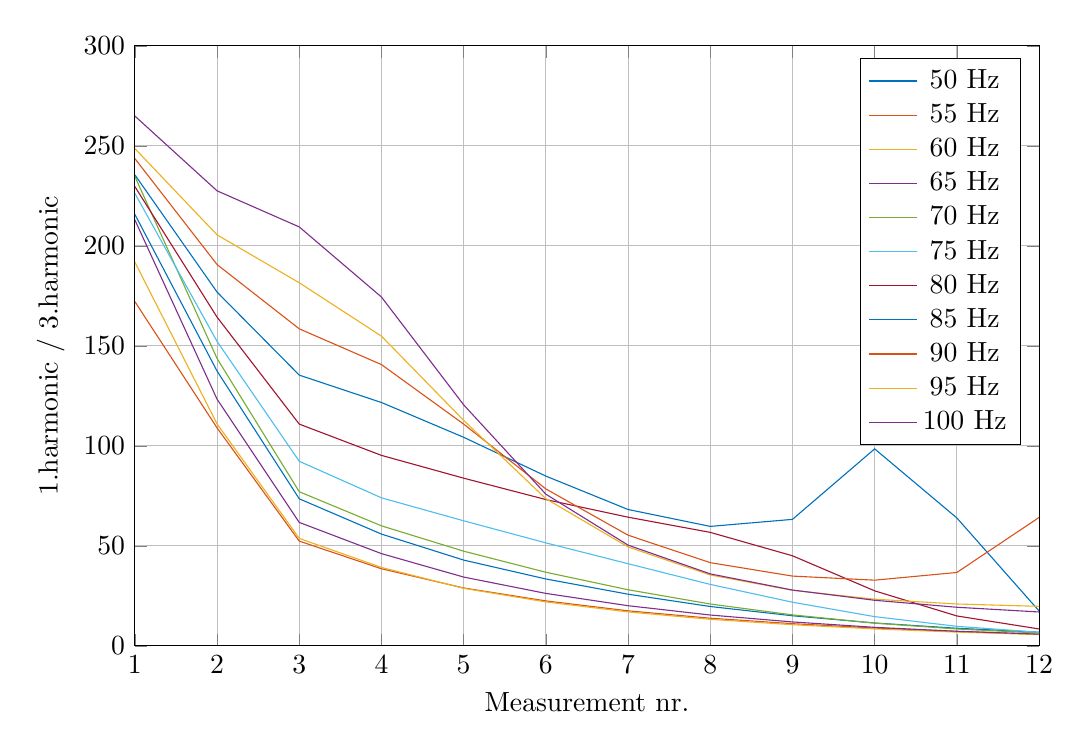
\begin{tikzpicture}

\begin{axis}[%
width=4.521in,
height=3in,
at={(0.758in,0.481in)},
scale only axis,
xmin=1,
xmax=12,
xmajorgrids,
ymin=0,
ymax=300,
ymajorgrids,
ylabel={1.harmonic / 3.harmonic},
xlabel={Measurement nr.},
axis background/.style={fill=white}
]
\addplot [color=mycolor1,solid]
  table[row sep=crcr]{%
1	215.719482689042\\
2	137.375839651914\\
3	73.491881974411\\
4	55.8600092831965\\
5	42.8578352198597\\
6	33.4172800378876\\
7	25.8045950665186\\
8	19.6476489187032\\
9	15.0203405516948\\
10	11.4021105008808\\
11	8.78151310064488\\
12	6.80575125314477\\
};
\addlegendentry{50 Hz};

\addplot [color=mycolor2,solid]
  table[row sep=crcr]{%
1	172.114474693239\\
2	108.959681506917\\
3	52.3472860469133\\
4	38.5211919605244\\
5	28.9212327445786\\
6	22.4544179872231\\
7	17.4931667868384\\
8	13.801173223079\\
9	11.0695402422613\\
10	8.86672628119122\\
11	7.18230155557047\\
12	5.85814167806323\\
};
\addlegendentry{55 Hz};

\addplot [color=mycolor3,solid]
  table[row sep=crcr]{%
1	191.855800187184\\
2	110.953017277433\\
3	53.683693987778\\
4	39.1905573675628\\
5	28.7432207660826\\
6	21.9384090830466\\
7	16.9403111162619\\
8	13.2430949708588\\
9	10.5478998664765\\
10	8.44228317755285\\
11	6.8502781275488\\
12	5.61256508528794\\
};
\addlegendentry{60 Hz};

\addplot [color=mycolor4,solid]
  table[row sep=crcr]{%
1	212.967593013927\\
2	123.29628240462\\
3	61.6977581937471\\
4	46.087964403812\\
5	34.3674120619029\\
6	26.2006981358897\\
7	20.0496847996708\\
8	15.3920698020736\\
9	11.9375533950336\\
10	9.2331507973757\\
11	7.26857819425135\\
12	5.81724097588744\\
};
\addlegendentry{65 Hz};

\addplot [color=mycolor5,solid]
  table[row sep=crcr]{%
1	234.702654081076\\
2	143.654071251651\\
3	77.0302711130303\\
4	59.9879332842773\\
5	47.3106009863147\\
6	36.7764664566778\\
7	28.0333423931352\\
8	20.8956209974193\\
9	15.4637596342843\\
10	11.3278856361071\\
11	8.40468415229921\\
12	6.38901276926542\\
};
\addlegendentry{70 Hz};

\addplot [color=mycolor6,solid]
  table[row sep=crcr]{%
1	226.209153737198\\
2	152.210426408944\\
3	92.2545328200555\\
4	73.9825383217611\\
5	62.5040084794028\\
6	51.4667509935922\\
7	41.049495369253\\
8	30.6957852407747\\
9	21.7968693650809\\
10	14.5785490688354\\
11	9.7443318755874\\
12	6.7525393990427\\
};
\addlegendentry{75 Hz};

\addplot [color=mycolor7,solid]
  table[row sep=crcr]{%
1	229.635293191795\\
2	164.339841957498\\
3	110.849225518279\\
4	95.2095843851408\\
5	83.8160696235361\\
6	73.1256889751953\\
7	64.3117819142494\\
8	56.7158231404608\\
9	45.0103733731685\\
10	27.480243912524\\
11	14.9274558888611\\
12	8.42340571546528\\
};
\addlegendentry{80 Hz};

\addplot [color=mycolor1,solid]
  table[row sep=crcr]{%
1	235.490142481433\\
2	176.874977155834\\
3	135.353253187891\\
4	121.654914199797\\
5	104.262795163307\\
6	84.8518375205328\\
7	68.153561437247\\
8	59.7049006381259\\
9	63.2192417248968\\
10	98.4705122104372\\
11	63.9227101729301\\
12	17.4365884138633\\
};
\addlegendentry{85 Hz};

\addplot [color=mycolor2,solid]
  table[row sep=crcr]{%
1	243.625116326288\\
2	190.625692275955\\
3	158.487616772918\\
4	140.613342268007\\
5	110.851821081734\\
6	78.4408481270658\\
7	55.3137703046313\\
8	41.567805737901\\
9	34.8603436700427\\
10	32.8193125376356\\
11	36.6722236082736\\
12	64.1801894559288\\
};
\addlegendentry{90 Hz};

\addplot [color=mycolor3,solid]
  table[row sep=crcr]{%
1	248.626858493455\\
2	205.485109505812\\
3	181.517854932663\\
4	154.824971458371\\
5	112.734503287044\\
6	73.5428507994872\\
7	49.4273612797893\\
8	35.4248581541094\\
9	27.7586461995489\\
10	23.3064114126667\\
11	20.9043305865742\\
12	19.7354496791802\\
};
\addlegendentry{95 Hz};

\addplot [color=mycolor4,solid]
  table[row sep=crcr]{%
1	264.893936681882\\
2	227.491544249115\\
3	209.43939847287\\
4	174.38343883648\\
5	120.48310284721\\
6	75.8068005942284\\
7	50.3376273635925\\
8	35.9571675595305\\
9	27.8773577027189\\
10	22.7572946932365\\
11	19.2742309190579\\
12	16.9124632980934\\
};
\addlegendentry{100 Hz};

\end{axis}
\end{tikzpicture}%
    \caption{1.harmonic / 3.harmonic pr. measurement. comparison for all frequencies}
\label{fig:com_mic13All_repport}
\end{figure}  

\autoref{fig:com_mic13All_repport} show that the third harmonic increases with the amplifiers gain. From this information it is possible to determine the speakers behaviour according to the gain and thereby use it is a model for gain adjustment.




\subsubsection{Plausible solution} 
The Previous tests have shown that it is possible to use an accelerometer to estimate the performance of the system by looking at the harmonic distortions. However following up on all of the trails the problems are as follows:
\begin{itemize}
\item Estimating harmonic distortions introduced in a system when playing music, are only well-defined for periodic sinusoids.
\item Frequency response of vibration, using the cheaper accelerometer, on the driver and cabinet hardly changes when exposed for loud playback, thus it will be hard to get usable outputs of the sensors.
\item The price for usable sensor equipment is too high compared to the application it is targeted for. 
\item The sensors did not directly show a pattern for when a possible hit of the back plate were about to occur.
\item The phase of the signal can not assumed "in phase" and it is therefore not possible to apply spectral estimations for detecting specific frequency peaks. e.g. if using a specific frequency as target for attenuation a 180 degrees phase shifted signal might bring false negatives. 
\end{itemize}

It can therefore be concluded that developing a system based on measurements from a accelerometer might turn out to be too complex to be realized in time due to time constraints. The system to be designed will therefore be based on a feedforward system. The concept of a feedforward system which fulfill the problem statement is shown in \autoref{fig:Concept}.

\begin{figure}[H]
\centering
\tikzsetnextfilename{Concept}
\scalebox{0.8}{
\begin{tikzpicture}
%% Kasser %%
\node [block, fill=black!80,text=white] (AudioSource) at (0,0) {Audio Source};

%% DSP %%
\node [block, fill=blue!15] (Equalizer1) at ($(AudioSource)+(3.5,0)$) {Equalizer};
\node [block, fill=blue!15] (SpectralAnalysis) at ($(Equalizer1)+(3.5,0)$) {Signal analysis};
\node [block, fill=blue!15] (Equalizer) at ($(SpectralAnalysis)+(4.5,0)$) {Signal processing};


%% External %%
\node [block, fill=blue!15] (UserInterface) at ($(Equalizer1)+(-3.5,2)$) {User interface};
\node [block, fill=blue!15] (UserInterfaceDev) at ($(Equalizer1)+(3.5,2)$) {Developer interface};

%% Speaker Enclosure %%
\node [block, fill=black!80,text=white] (Amplifier) at ($(SpectralAnalysis)+(4.5,-3)$) {Amplifier};
\node [block, fill=black!80,text=white] (Driver) at ($(Amplifier)+(-3.5,0)$) {Driver};

\node (User) at ($(-2.5,0)+(UserInterface)$) {\textbf{User}};
\node (Developer) at ($(3.6,0)+(UserInterfaceDev)$) {\textbf{Developer}};
\draw[->] (User) -- (UserInterface);
\draw[->] (Developer) -- (UserInterfaceDev);

% Store Blokke %%
\begin{pgfonlayer}{bg}
\draw[thick, fill=black!10] ($(-1.75,1.2)+(Equalizer1)$) -- ($(2.5,1.2)+(Equalizer)$) -- ($(2.5,-1.5)+(Equalizer)$) -- ($(-1.75,-1.5)+(Equalizer1)$) -- ($(-1.75,1.2)+(Equalizer1)$);
\node (DSPtag) at ($(0,-1.1)+(SpectralAnalysis)$) {\textbf{Digital Processing System}};

\draw[thick, fill=black!10] ($(-2.5,1)+(Driver)$) -- ($(2.5,1)+(Amplifier)$) -- ($(2.5,-1.5)+(Amplifier)$) -- ($(-2.5,-1.5)+(Driver)$) -- ($(-2.5,1)+(Driver)$);
\node (DSPtag) at ($(2,-1.1)+(Driver)$) {\textbf{Speaker Enclosure}};
\end{pgfonlayer}

%% Forbindelse %%
\draw[->] (AudioSource) -- (Equalizer1);
\draw[->] (Equalizer1) -- (SpectralAnalysis);
\draw[->] (SpectralAnalysis) -- (Equalizer);
\draw[->] (Equalizer) -- (Amplifier);
\draw[->] (Amplifier) -- (Driver);

\draw[->] (UserInterface) -| ($(Equalizer1)+(-.25,.6)$);
\draw[->] (UserInterfaceDev) -| ($(Equalizer1)+(.25,.6)$);

%\draw[->] ($(SensorDriver)+(-1.375,-0.3)$) -- ($(SpectralAnalysis)+(1.375,-0.3)$);

%\draw[->] (SpectralAnalysis) -- (Decisionblock);
%\draw[->] (Decisionblock) |- (Equalizer);
\end{tikzpicture}}
\caption{Overview of a feedforward design concept.}
\label{fig:Concept}
\end{figure}

Since the system will be controlled using a feedforward system which should be able to analyze, process and correct signals before the music is played. It gives rise to questioning what kind of platform should be used and what kind of requirements are needed for such a system. On the market there are different plausible platforms which meets with the demands all with different advantages and disadvantages. The preceding section will cover the determination of which platform that will function best in a active loudspeaker system . 

%\textbf{The design concept consist of a signal processing block, which will be analysed to understand which solution is best for the problem stated. A signal analysis block which will not be analysed further in this chapter, a user interface which will be analysed to determine how the user interface should be designed and lastly the processor block which will be analysed to determine which type of processor that should be used.}



%% Krav til Platform %%
\section{Platform requirements} \label{sec:platformReq}
The purpose of this section is to derive the requirements for the digital development platform. Most of the requirements derived in this section are provided by DALI thus the choice of platform will mostly be based on an analysis of which processor platform will be optimal in order to fulfill the requirements. The requirements for the processor platform have been derived in a mail correspondence with DALI.
\todo[inline]{Reference til CD}
%\subsection*{Demands for the platform}
%The demands for the processor platform have been derived in a mail correspondence with DALI 
%\todo[inline]{Reference til CD}
\begin{itemize}
\item \textbf{Audio sample rate}: The system must be able to handle 96 kHz sample rate since peripheral components will be running at this rate.
\item \textbf{Audio resolution}: There must be support for audio in at least a 24 bit resolution since the \gls{DAC} chosen by DALI is of 24 bit.
\item \textbf{\gls{SNR}}: A minimum \gls{SNR} of 120 dB on the \gls{DAC} must be achieved. This will provide headroom for digital volume control.
\item \textbf{Performance}: The processor must a least be able to run 1024 instructions per sample. which would give approximately 100 \gls{MIPS}.
%\item \textbf{Program space}: The platform will consist of an equalizer and limiter when finished. This project will however focus on the equalizer and sensory system. Hence it only desireable to leave TBD room for an multi band limiter which is desired by DALI. 
\item \textbf{Interfacing to peripherals}: The platform must be able to interface with an ADC and DAC with the bus type \gls{I2S}.

\todo[inline]{Program space has been removed.}

A 32 bit resolution is prefered by DALI over a 24 bit resolution because it would give a increased \gls{SNR} of 48 dB. These demands lead to the analyzation of which platform would be the most optimal.  
\end{itemize}


%\subsection*{Sample rate} 
%The system must be able to handle 96 kHz sample rate since peripheral components will interface be running at this rate.
%
%\subsection*{Bit resolution} 
%There must be support for audio in at least a 24 bit resolution since the \gls{DAC} chosen by DALI is of 24 bit.
%
%\subsection*{\gls{SNR}} 
%A minimum \gls{SNR} of 120 dB on the \gls{DAC} must be achieved. This will provide headroom for digital volume control.
%
%\subsection*{Instructions pr. sample.} 
%The processor must a least be able to run 1024 intructions pr. sample. which would give approximately 100 \gls{MIPS}
%
%
%\subsection*{Memory for both an equalizer and multi band limiter} 
%The platform will consist of an equalizer and limiter when finished. This project will however focus on the equalizer and sensory system. Hence it only desireable to leave TBD room for an multi band limiter which is desired by DALI. 
%
%
%\subsection*{Interfacing} 
%The platform must be able to interface with an ADC and DAC with the bus type \gls{I2S}. Besides the interfacing with the ADC and DAC the platform must be able to interface with the chosen sensor in \autoref{sec:Sensor}.
%
%The 32 bit resolution is prefered by DALI over a 24 bit resolution because it would give a increased \gls{SNR} of 48 dB. These demands lead to the analyzation of which platform would be the most optimal.   

\subsection{Choice of processor platform}
For the choice of processor platform different types of platforms could be used, such as an ASIC chip, an \gls{FPGA}, a microcontroller ($\mu$C) or a \gls{DSP}. These types of processors have different advantage and disadvantages which needs to be analyzed to find the most optimal platform for the demands above. The basic difference between the types of platforms is given in \autoref{tb:summary_DSP_hardware_implementation}. 

\begin{table}[H]
\centering
\begin{tabular}{lllll}
\toprule
 & \multicolumn{1}{c}{ASIC} & \multicolumn{1}{c}{FPGA} & \multicolumn{1}{c}{$\mu$P/$\mu$C} & \multicolumn{1}{c}{\begin{tabular}[c]{@{}c@{}}Digital signal\\ processor\end{tabular}} \\ \hline
\textbf{Flexibility} & None & Limited & High & High \\
\textbf{Design time} & Medium & Medium & Short & Short \\
\textbf{Power consumption} & Low-medium & Medium-high & Medium high & Low-medium \\
\textbf{Performance} & High & Low-medium & Low-medium & Medium-high \\
\textbf{Development cost} & Medium & Low & Low & Low \\ 
\textbf{Production cost} & Low-medium & Medium-high & Medium-high & Low-medium \\ \bottomrule 
\end{tabular}
\caption{Summary of DSP hardware implementations \citep{WileyDSP}.}
\label{tb:summary_DSP_hardware_implementation}
\end{table}


Because filtering is probably needed and the high performance demands from above the natural choice of platform would be a \gls{DSP}. An ASIC chip would not be viable as a prototype platform because it does not have any flexibility. The FPGA lacks flexibility, has an increased design time and is costly. The microcontroller has less performance than a \gls{DSP}, cost more and normally has a bigger power consumption than a \gls{DSP} so as stated before a \gls{DSP} is the choice of platform.     






%% GUI %%
%\section{User interface} \label{sec:user_interface}
In this section an analyzation of the user interface for the equalizer analyzed in \autoref{sec:tech_equalizer} will be made to determine which user interface will be the most optimal for the specific user of the equalizer. 

There are two different intended users for the equalizer: 
\begin{itemize}
\item The developer.
\item The commercial user.
\end{itemize}
This means that there are different requirements for the specific user of the equalizer.

\subsection*{User interface for the developer}
The developer is the user which knows everything about an equalizer and its effects on a system therefore the developer desires a great deal of control and options in the interface of the equalizer. This means that the interface can be complex and must not set no restrictions for the developer.  

Because the developer needs to have full control of the equalizer he needs to have control of: 
\begin{itemize}
\item Center frequency.
\item Q - value.
\item Gain.
\item Band selection.
\end{itemize} 
This leads to a suggestions for a user interface which gives full control to a developer.

\begin{figure}[H]
\centering
\tikzsetnextfilename{InterfaceDev1}
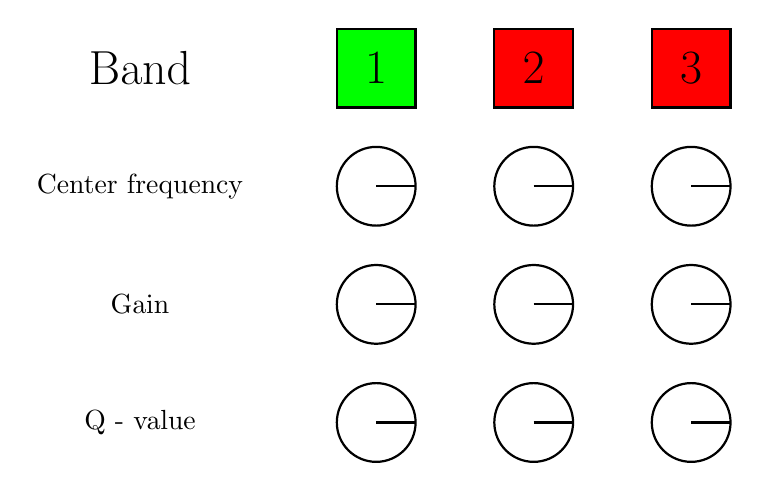
\begin{tikzpicture}
\draw[thick] (2,0) circle [radius=0.5] node at (-1,-0) {Q - value};
\draw[thick] (2,1.5) circle [radius=0.5] node at (-1,1.5) {Gain};
\draw[thick] (2,3) circle [radius=0.5] node at (-1,3) {Center frequency};
\draw node at (-1,4.5)[font=\LARGE]{Band};
\draw[thick][fill=green, draw=black](1.5,4) rectangle(2.5,5) node at (2,4.5)[font=\LARGE]{1};

\draw[thick] (4,0) circle [radius=0.5];
\draw[thick] (4,1.5) circle [radius=0.5];
\draw[thick] (4,3) circle [radius=0.5];
\draw[thick][fill=red, draw=black](1.5+2,4) rectangle(2.5+2,5) node at (2+2,4.5)[font=\LARGE]{2};

\draw[thick] (6,0) circle [radius=0.5];
\draw[thick] (6,1.5) circle [radius=0.5];
\draw[thick] (6,3) circle [radius=0.5];
\draw[thick][fill=red, draw=black](1.5+4,4) rectangle(2.5+4,5) node at (2+4,4.5)[font=\LARGE]{3};

\draw[thick](6,0) -- (6.5,0);
\draw[thick](6,1.5) -- (6.5,1.5);
\draw[thick](6,3) -- (6.5,3);

\draw[thick](4,0) -- (4.5,0);
\draw[thick](4,1.5) -- (4.5,1.5);
\draw[thick](4,3) -- (4.5,3);

\draw[thick](2,0) -- (2.5,0);
\draw[thick](2,1.5) -- (2.5,1.5);
\draw[thick](2,3) -- (2.5,3);
\end{tikzpicture}
\caption{Developer user interface.}
\label{fig:Dev_sug}
\end{figure}

The suggestion on \autoref{fig:Dev_sug} has push buttons on the bands so they can be toggled on and of while the center frequency, gain and Q - value for each band can be changed with the use of knobs. 

\subsection*{User interface for the commercial user}
The commercial user is the user which knows the implication of different the different settings of an equalizer but does not know anything about the technical aspect of an equalizer. This means that the interface needs to be simple and show what implpication a setting has on a system but leave out all technical aspects. 

Because the commercial user only needs presets like for example "rock", "jazz" and "movie" the user only needs to have control of: 
\begin{itemize}
\item Presets.
\end{itemize} 
This leads to some different suggestions for a user interface which consist of a few buttons to keep it as simple as possible.


\begin{figure}[H]
\centering
\begin{subfigure}[t]{0.47\textwidth}
	\centering
	\tikzsetnextfilename{InterfaceUser1}
	\scalebox{0.2}{
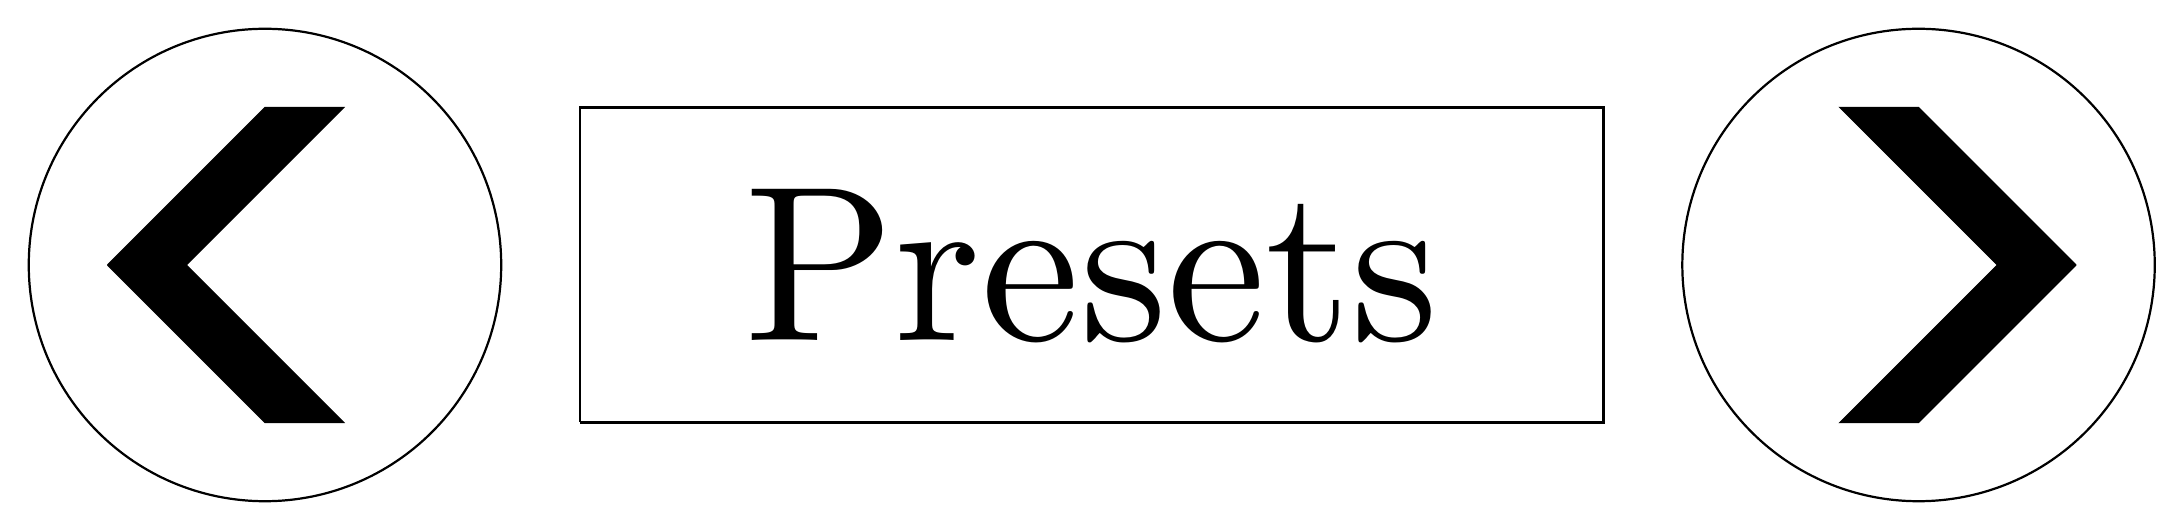
\begin{tikzpicture}
\draw [thick](-10,6) circle [radius=3];
\draw [thick](11,6) circle [radius=3];
\draw [thick](-6,4) -- (7,4) -- (7,8) -- (-6,8) -- (-6,4);
\draw[fill] (-12,6) -- (-10,8) -- (-9,8) -- (-11,6) -- (-9,4) -- (-10,4) -- (-12,6);
\draw[fill](13,6) -- (11,8) -- (10,8) -- (12,6) -- (10,4) -- (11,4)--(13,6) ;
\node[scale=8.0] (c) at (0.5,6) {Presets};
\end{tikzpicture}}
	\caption{Suggestion 1}
	\label{fig:UI_sug_1}
\end{subfigure}
\hspace{6mm} 
\begin{subfigure}[t]{0.47\textwidth}
	\centering
	\tikzsetnextfilename{InterfaceUser2}
	\scalebox{0.6}{
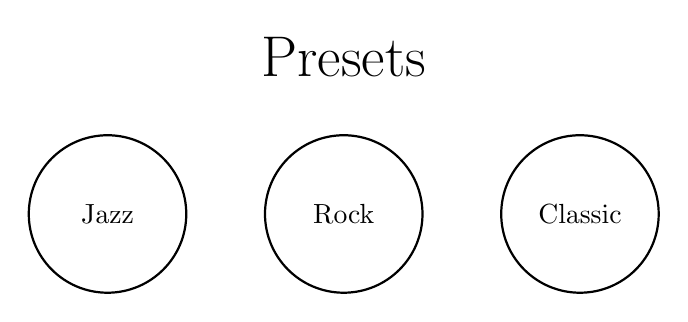
\begin{tikzpicture}
\draw [thick](0,0) circle [radius=1] node{Jazz};
\draw [thick](3,0) circle [radius=1] node{Rock};
\draw [thick](6,0) circle [radius=1] node{Classic};
\draw node at (3,2)[font=\huge]{Presets};
\end{tikzpicture}}
	\caption{Suggestion 2}
	\label{fig:UI_sug_2}
\end{subfigure}
\caption{Commercial user interface suggestions.}
\label{fig:UI_sug}
\end{figure}

Suggestion one as seen on \autoref{fig:UI_sug_1} has two push buttons and a small screen so the user can interchange between different settings, while suggestion two has x number of push buttons which represents a preset each. The advantage of suggestion two is the overview and simplicity while suggestion one can have a larger number of presets without changing the appearance of the user interface. 

The suggestions for the user interface for both the developer and the commercial user will be choosen in the requirement specification \todo[inline]{reference}  

